% =====================================================================
% 文档类选项（ElegantBook 4.7）
%   lang=cn          中文环境      scheme=chinese  章号用中文数字
%   toc=twocol       双栏目录      section         定理类环境按节编号（thmcnt=section）
%   chinesefont=nofont  自行设置中文字体（见下方 \setCJK... 命令）
%   未声明 mode，即默认 fancy 模式；未声明 math，即默认 cm 数学字体（模板推荐）
% =====================================================================
\documentclass[lang=cn,10.5pt,scheme=chinese,toc=twocol,section,chinesefont=nofont,
citestyle=gb7714-2015,bibstyle=gb7714-2015]{elegantbook}

\title{高等代数讲义}
\subtitle{非数学专业“线性代数”课程选用}

\author{卢米埃尔 // Lumiere}
% ---------- 版本与日期（全书唯一来源） ----------
% 版本号发布新版时手动修改；日期由 CI 写入 version.tex（= 最后一次提交的日期），
% 本地编译没有该文件时退回当天日期。封面、标题页、版权页都只用这两个命令。
\newcommand{\noteversion}{0.10}
\InputIfFileExists{version}{}{\newcommand{\notedate}{\zhtoday}}
\date{\notedate}
\version{\noteversion}
\bioinfo{作者主页}{lumierelp.github.io}

\extrainfo{攀登山顶的拼搏本身足以充实一颗人心。我们应当想象西西弗斯是幸福的。}

\setcounter{tocdepth}{2}

\cover{cover.png}

\newif\ifprintversion
\printversionfalse   % 交印厂：true；电子版：改成 \printversionfalse

\ifprintversion
\geometry{
	paperwidth   = 191mm,  paperheight  = 266mm,   % 含出血的画布
	layoutwidth  = 185mm,  layoutheight = 260mm,   % 成品尺寸
	layouthoffset = 3mm,   layoutvoffset = 3mm,    % 居中，四边各留 3mm
	left = 20mm, right = 18mm, top = 22mm, bottom = 20mm,
	headsep = 3mm, footskip = 8mm
}
\else
\geometry{
	paperwidth = 185mm, paperheight = 260mm,
	left = 20mm, right = 18mm, top = 22mm, bottom = 20mm,
	headsep = 3mm, footskip = 8mm
}
\fi
\AtBeginDocument{\setlength{\headwidth}{\textwidth}}

% ==================== 本文档命令 ====================
\usepackage{array}
\usepackage{nicematrix}
\newcommand{\ccr}[1]{\makecell{{\color{#1}\rule{1cm}{1cm}}}}
\setCJKmainfont[BoldFont={NotoSerifCJKsc-Bold.otf},ItalicFont={FZKTK.TTF},BoldItalicFont={NotoSerifCJKsc-Bold.otf}]{FZSSK.TTF}
% ---------- 字体 ----------
\setmainfont{cmunrm.otf}[BoldFont=cmunbx.otf, ItalicFont=cmunti.otf, BoldItalicFont=cmunbi.otf]
\setsansfont{cmunss.otf}[BoldFont=cmunsx.otf, ItalicFont=cmunsi.otf]
\setmonofont{cmuntt.otf}[BoldFont=cmuntb.otf, ItalicFont=cmunit.otf]
\setCJKsansfont[BoldFont={NotoSansCJKsc-Black.otf}]{NotoSansCJKsc-Regular.otf}
\setCJKmonofont[BoldFont={NotoSansMonoCJKsc-Regular.otf}]{NotoSansMonoCJKsc-Regular.otf}
\setCJKfamilyfont{zhsong}{NotoSerifCJKsc-Regular.otf}
\setCJKfamilyfont{zhhei}{NotoSansCJKsc-Regular.otf}
\setCJKfamilyfont{zhkai}[BoldFont={NotoSansCJKsc-Regular.otf}]{FZKTK.TTF}
\setCJKfamilyfont{zhfs}[BoldFont={NotoSansCJKsc-Regular.otf}]{FZFSK.TTF}
\newcommand*{\songti}{\CJKfamily{zhsong}}
\newcommand*{\heiti}{\CJKfamily{zhhei}}
\newcommand*{\kaishu}{\CJKfamily{zhkai}}
\newcommand*{\fangsong}{\CJKfamily{zhfs}}
% 封面叠加文字用的字体：数字等西文用 Montserrat Regular（TeX Live 自带 montserrat 宏包），
% 中文用思源黑体同字形的 Noto Sans CJK
\newfontfamily\coverlatinfont{Montserrat-Regular.otf}
\newCJKfontfamily\covercjkfont{NotoSansCJKsc-Regular.otf}
\newcommand*{\coverinfofont}{\coverlatinfont\covercjkfont\fontsize{10.2pt}{12pt}\selectfont}
% 修改标题页的橙色带
\definecolor{customcolor}{RGB}{104,200,240}
\colorlet{coverlinecolor}{customcolor}
\usepackage{cprotect}
\usepackage{tikz}
\usetikzlibrary{arrows.meta,calc,angles,quotes,decorations.pathreplacing}
\colorlet{figblue}{customcolor!75!black}
\colorlet{figorange}{orange!85!black}
\colorlet{figred}{red!70!black}
\colorlet{figgreen}{green!45!black}
\colorlet{figviolet}{violet!70!black}
\tikzset{
	>={Stealth[length=2mm]},
	vec/.style={->,thick},
	axis/.style={->,gray!70,thin},
	dot/.style={circle,fill,inner sep=1.2pt},
	station/.style={circle,draw=figblue,fill=customcolor!15,thick,
		minimum size=7mm,inner sep=1pt},
	sub/.style={font=\small,align=center},
	iso/.style={x={(-0.55cm,-0.42cm)},y={(1cm,0cm)},z={(0cm,1cm)}},
	iso2/.style={x={(0.35cm,-0.5cm)},y={(1cm,0.1cm)},z={(0cm,1cm)}},
}
% ---------- 全书统一记号 ----------
% 向量与矩阵一律用加粗斜体
\newcommand{\vv}[1]{\boldsymbol{#1}}
\newcommand{\zero}{\boldsymbol{0}}          % 零向量（全书统一，不再混用 \mathbf{0}）
\newcommand{\trans}{\mathrm{T}}             % 转置：A^{\trans}
\newcommand{\spn}{\operatorname{span}}      % 张成：\spn(\vv\alpha_1,\ldots)
\newcommand{\rk}{\operatorname{rank}}       % 秩
\newcommand{\imm}{\operatorname{Im}}        % 像
\newcommand{\diag}{\operatorname{diag}}
\providecommand{\tr}{\operatorname{tr}}     % 迹（正文、习题与答案统一使用）

% ---------- 学时标记（含义见``本书记号约定''） ----------
% 不加标记：48 学时方案即讲授；\hB：64 学时及以上讲授；\hC：72 学时讲授；* ：选读.
\newcommand{\hB}{\texorpdfstring{\textdagger}{†}}
\newcommand{\hC}{\texorpdfstring{\textdaggerdbl}{‡}}
\newcommand{\chapterhours}[3]{%
	\par\smallskip\noindent{\small\sffamily 建议学时：48 学时方案 #1\quad 64 学时方案 #2\quad 72 学时方案 #3}\par\smallskip}

% ---------- 索引与长表格 ----------
% 索引条目用 \index{拼音@中文} 的形式按拼音排序；编译时需运行 makeindex
% （imakeidx 在 -shell-escape 或受限 shell-escape 下会自动调用，latexmk 也会处理）.
\usepackage{imakeidx}
\makeindex[intoc,columns=2,title=索引,options=-l]
\usepackage{longtable}

% ---------- 自定义定理类环境 ----------
% 模板自带的 property 属于``结论类环境''，不编号、不能 \ref。
% 行列式的性质需要编号和引用，故用模板提供的 \elegantnewtheorem 另建一个。
% fancy 模式用法：\begin{dprop}{名字}{标签} ... \end{dprop}，引用写 \ref{prop:标签}
\elegantnewtheorem{dprop}{性质}{prostyle}{prop}

% ---------- 证毕符号 ----------
% 模板 v4.5 的 proof 环境注释掉了结束符号，这里统一补上
\AtEndEnvironment{proof}{\nobreak\hfill$\blacksquare$}
% \xlongequal 来自 extarrow 宏包；若模板未加载，用下面的备用定义
\providecommand{\xlongequal}[2][]{\mathrel{\overset{#2}{\underset{#1}{=\joinrel=\joinrel=}}}}

% ---------- 特色栏目 ----------
\usepackage{tcolorbox}
\tcbuselibrary{breakable,skins}
\newtcolorbox{motivebox}{breakable,enhanced,colback=customcolor!6,colframe=customcolor!70!black,
	fonttitle=\bfseries\sffamily,title={思维动机}}
\newtcolorbox{linkbox}[1]{breakable,enhanced,colback=orange!5,colframe=orange!65!black,
	fonttitle=\bfseries\sffamily,title={专业连线：#1}}
\newtcolorbox{historybox}[1]{breakable,enhanced,colback=gray!5,colframe=gray!60!black,
	fonttitle=\bfseries\sffamily,title={历史回响：#1}}
\newtcolorbox{pitfallbox}{breakable,enhanced,colback=red!4,colframe=red!55!black,
	fonttitle=\bfseries\sffamily,title={常见误区}}
\newtcolorbox{codebox}[1]{breakable,enhanced,colback=green!3,colframe=green!45!black,
	fonttitle=\bfseries\sffamily,title={计算实践：#1}}
\newtcolorbox{modelbox}[1]{breakable,enhanced,colback=violet!4,colframe=violet!60!black,
	fonttitle=\bfseries\sffamily,title={建模实验：#1}}
\newcommand{\mstep}[1]{\par\smallskip\noindent\textbf{【#1】}\ }
\usepackage{caption}
\usepackage{listings}
\lstset{language=Python,basicstyle=\ttfamily\small,columns=fullflexible,
	breaklines=true,keepspaces=true,showstringspaces=false}
%% =====================================================================
%% exercises.tex　《高等代数讲义》章末习题（A/B/C 三组）
%%
%% 用法
%%   1. 在导言区（\begin{document} 之前、全书统一记号之后）写 %% =====================================================================
%% exercises.tex　《高等代数讲义》章末习题（A/B/C 三组）
%%
%% 用法
%%   1. 在导言区（\begin{document} 之前、全书统一记号之后）写 %% =====================================================================
%% exercises.tex　《高等代数讲义》章末习题（A/B/C 三组）
%%
%% 用法
%%   1. 在导言区（\begin{document} 之前、全书统一记号之后）写 \input{exercises}.
	%%   2. 在每章末尾（原 \begin{problemset}...\end{problemset} 之后，或替换它）
	%%      写对应的命令：
	%%        第一章 \ExElimination      第二章 \ExVectorSpace   第三章 \ExMatrix
	%%        第四章 \ExLinearMap        第五章 \ExDeterminant   第六章 \ExSolutions
	%%        第七章 \ExPolynomial       第八章 \ExEigen         第九章 \ExInnerProduct
	%%        第十章 \ExDecomposition    第十一章 \ExQuadratic   第十二章 \ExBilinear
	%%   3. 分组标准
	%%        A 组：直接运用本章定义与定理的计算和证明；
	%%        B 组：需要综合多个结论、或有一定技巧的计算和证明；
	%%        C 组：有挑战性的题目，或超出本课程大纲、为继续深造准备的内容.
	%%   4. 题目与正文中已有的节末练习、原 problemset 不重复；个别题目注明``接正文某题''.
	%%      第六章按扩充版（ch06-solutions.tex）的内容编写.
	%%   5. 每道题都带标签 ex:<章键>:<组号>，正文、习题与附录答案一律用 \ref 引用，
	%%      渲染为``A4''``B12''这样的题号. 章键依次为
	%%        elim vs mat lmap det sol poly eig ip dec quad bil（第一至十二章）.
	%%      例：第一章章末习题~\ref{ex:elim:B12}. 新增题目请加在组末，并补上标签.
	%%      A 组答案、B 组提示在 answers.tex 中，按同一标签对应.
	%% 依赖：导言区的 \vv \zero \trans \spn \rk \imm \diag，以及 enumitem（elegantbook 已加载）.
	%% 引用的前文标签：thm:sameSolution thm:solvability prop:linspc eg:pricedecomp cor:homogeneous thm:rouche thm:sol-determinable
	%%   thm:spectral thm:posdef thm:svd thm:orthcanon
	%% =====================================================================
	
	\providecommand{\tr}{\operatorname{tr}}
	\newcommand{\exsetheading}{%
		\section*{章末习题}%
		\markright{章末习题}%
	}
\newcommand{\exgroup}[2]{%
	\par\medskip{\centering\sffamily\bfseries #1\quad #2\par}\smallskip}
	\newenvironment{exA}{\begin{enumerate}[label=\textbf{A\arabic*.},ref=A\arabic*,leftmargin=2.8em,itemsep=4pt]}{\end{enumerate}}
	\newenvironment{exB}{\begin{enumerate}[label=\textbf{B\arabic*.},ref=B\arabic*,leftmargin=2.8em,itemsep=4pt]}{\end{enumerate}}
	\newenvironment{exC}{\begin{enumerate}[label=\textbf{C\arabic*.},ref=C\arabic*,leftmargin=2.8em,itemsep=4pt]}{\end{enumerate}}
	\newcommand{\Agroup}{\exgroup{A 组}{基础巩固}}
	\newcommand{\Bgroup}{\exgroup{B 组}{综合提升}}
	\newcommand{\Cgroup}{\exgroup{C 组}{拓展探索}}
	
	% =====================================================================
	% 第一章　线性方程组与消元法
	% =====================================================================
	\newcommand{\ExElimination}{%
		\exsetheading
		\Agroup
		\begin{exA}
			\item\label{ex:elim:A1} 判断下列矩阵哪些是阶梯形，哪些是简化阶梯形：
			\[
			\begin{pmatrix}1&2&0\\0&0&1\end{pmatrix},\quad
			\begin{pmatrix}1&0&3\\0&2&1\\0&0&0\end{pmatrix},\quad
			\begin{pmatrix}0&1&0\\1&0&0\end{pmatrix},\quad
			\begin{pmatrix}1&0&2&0\\0&1&-1&0\\0&0&0&1\end{pmatrix},\quad
			\begin{pmatrix}0&0\\0&1\end{pmatrix}.
			\]
			\item\label{ex:elim:A2} 写出方程组 $3x_1-x_3=2$，$x_2+4x_3=0$，$x_1-x_2=5$ 的增广矩阵；反过来，写出以 $\begin{pmatrix}1&-2&0&3\\0&1&5&-1\end{pmatrix}$ 为增广矩阵的方程组.
			\item\label{ex:elim:A3} 用消元法解方程组 $\left\{\begin{array}{l}x_1+2x_2+3x_3=14,\\2x_1-x_2+x_3=3,\\3x_1+x_2-x_3=2.\end{array}\right.$
			\item\label{ex:elim:A4} 用消元法解方程组 $\left\{\begin{array}{l}x_1+x_2+x_3+x_4=2,\\x_1-x_2+x_3-x_4=4,\\2x_1+x_2-x_3+3x_4=-1,\\x_1+2x_2+3x_3-2x_4=5.\end{array}\right.$
			\item\label{ex:elim:A5} 判断方程组 $\left\{\begin{array}{l}x_1-x_2+x_3=1,\\2x_1+x_2-x_3=2,\\x_1+2x_2-2x_3=3\end{array}\right.$ 是否有解，并说明消元过程中哪一行``暴露''了结论.
			\item\label{ex:elim:A6} 求方程组 $\left\{\begin{array}{l}x_1+2x_2-x_3+x_4=3,\\2x_1+4x_2-x_3+3x_4=7,\\-x_1-2x_2+2x_3=-2\end{array}\right.$ 的全部解，并指出主变量与自由变量.
			\item\label{ex:elim:A7} 求齐次方程组 $\left\{\begin{array}{l}x_1+x_2-x_3-x_4=0,\\2x_1-5x_2+3x_3+2x_4=0,\\7x_1-7x_2+3x_3+x_4=0\end{array}\right.$ 的全部解.
			\item\label{ex:elim:A8} 把矩阵 $\begin{pmatrix}2&4&-2&6\\1&2&1&1\\3&6&1&5\end{pmatrix}$ 化为简化阶梯形，并写出每一步所用的初等行变换.
			\item\label{ex:elim:A9} 写出全部 $2\times2$ 简化阶梯形矩阵的``形状''（可以含参数），并说明共有几类.
			\item\label{ex:elim:A10} $k$ 取何值时，方程组 $x+y=1$，$x-y=3$，$2x+ky=5$ 有解？
			\item\label{ex:elim:A11} 设 $a,b$ 为常数. 方程组 $x+2y=a$，$3x+6y=b$ 何时有解？有解时写出全部解.
			\item\label{ex:elim:A12} 求过三点 $(1,2)$，$(2,3)$，$(3,6)$ 的抛物线 $y=ax^2+bx+c$.
			\item\label{ex:elim:A13} 求过四点 $(-1,2)$，$(0,1)$，$(1,0)$，$(2,5)$ 的三次多项式函数 $y=a+bx+cx^2+dx^3$.
			\item\label{ex:elim:A14} 某剧场三种票价分别为 $30$，$50$，$80$ 元. 某场演出共售出 $100$ 张票，票房 $4800$ 元，且 $80$ 元票的张数恰为 $30$ 元票的一半. 三种票各售出多少张？
			\item\label{ex:elim:A15} 配平化学方程式 $x_1\,\mathrm{C_3H_8}+x_2\,\mathrm{O_2}\to x_3\,\mathrm{CO_2}+x_4\,\mathrm{H_2O}$：对 C，H，O 三种原子分别写出守恒方程，解这个齐次方程组，并取最小的正整数解.
			\item\label{ex:elim:A16} 某城区四个路口 $A,B,C,D$ 由单行道依次连成环路 $A\to B\to C\to D\to A$，环路上的车流量依次记为 $x_1$（$A\to B$），$x_2$（$B\to C$），$x_3$（$C\to D$），$x_4$（$D\to A$）（单位：辆/小时）. 各路口与外部道路的进出量为：$A$ 驶入 $400$、驶出 $300$；$B$ 驶入 $200$、驶出 $350$；$C$ 驶入 $250$、驶出 $100$；$D$ 驶入 $150$、驶出 $250$. 设每个路口驶入总量等于驶出总量.
			\begin{enumerate}
				\item 列出方程组并求全部解；
				\item 若各路段车流量都不能为负，$x_1$ 最少是多少？
				\item 若把 $D$ 的驶出量改为 $350$，方程组会怎样？这反映了什么守恒律？
			\end{enumerate}
			\item\label{ex:elim:A17} 证明：二元一次方程组 $ax+by=e$，$cx+dy=f$ 对任意的 $e,f$ 都有唯一解，当且仅当 $ad-bc\ne0$.（只用消元法，不用行列式.）
			\item\label{ex:elim:A18} 证明：若线性方程组有两个不同的解 $\vv x_1,\vv x_2$，则对任意数 $t$，$\vv x_1+t(\vv x_2-\vv x_1)$ 都是解. 由此说明：线性方程组的解要么不存在，要么唯一，要么有无穷多个.
			\item\label{ex:elim:A19} 证明方程组 $\{x+y+z=3,\ x-y=0\}$ 与 $\{2x+z=3,\ x+y+z=3\}$ 同解.
			\item\label{ex:elim:A20} 举例说明：若\textbf{同时}做``第一个方程加到第二个方程上''与``第二个方程加到第一个方程上''（两步都用原来的方程），所得方程组可能与原方程组不同解. 这与定理~\ref{thm:sameSolution}（初等行变换不改变解集）矛盾吗？
			\item\label{ex:elim:A21} 已知一个方程组的增广矩阵化为阶梯形后为 $\begin{pmatrix}1&3&-1&2&0\\0&0&2&1&4\\0&0&0&0&a\end{pmatrix}$. 讨论 $a$ 取何值时方程组有解；有解时它有几个自由变量？
		\end{exA}
		
		\Bgroup
		\begin{exB}
			\item\label{ex:elim:B1} 讨论 $a,b$ 取何值时，方程组
			\[\left\{\begin{array}{l}x_1+x_2+x_3+x_4=0,\\x_2+2x_3+2x_4=1,\\-x_2+(a-3)x_3-2x_4=b,\\3x_1+2x_2+x_3+ax_4=-1\end{array}\right.\]
			有唯一解、无解、有无穷多解；有无穷多解时求出全部解.
			\item\label{ex:elim:B2} 讨论 $\lambda$ 取何值时，方程组
			$(1+\lambda)x_1+x_2+x_3=0$，$x_1+(1+\lambda)x_2+x_3=3$，$x_1+x_2+(1+\lambda)x_3=\lambda$
			有唯一解、无解、有无穷多解.
			\item\label{ex:elim:B3} 设 $n$ 个方程、$n$ 个未知量的方程组对应的齐次方程组只有零解. 证明：无论常数项取什么值，原方程组都有唯一解.（提示：考察简化阶梯形中主元的个数.）
			\item\label{ex:elim:B4} 证明：线性方程组无解，当且仅当可以把若干个方程分别乘以适当的数再相加，得到矛盾方程 $0=1$.
			\item\label{ex:elim:B5} 证明：交换两行这一初等变换，可以由``倍加''与``某行乘以 $-1$''这两类变换的组合实现. 由此说明三类初等行变换并不是``独立''的.
			\item\label{ex:elim:B6} 证明：若线性方程组的系数和常数项都是有理数，且它有实数解，则它一定有有理数解；若它的实数解唯一，则这个解就是有理数解.
			\item\label{ex:elim:B7} 讨论方程组
			\[x_1-x_2=a_1,\quad x_2-x_3=a_2,\quad\ldots,\quad x_{n-1}-x_n=a_{n-1},\quad x_n-x_1=a_n\]
			有解的充要条件，并在有解时求全部解.
			\item\label{ex:elim:B8} 讨论方程组
			\[x_1+x_2=a_1,\quad x_2+x_3=a_2,\quad\ldots,\quad x_{n-1}+x_n=a_{n-1},\quad x_n+x_1=a_n\]
			的解. 证明：$n$ 为奇数时解唯一；$n$ 为偶数时有解当且仅当 $a_1-a_2+a_3-\cdots-a_n=0$.
			\item\label{ex:elim:B9} 某经济体有三个部门，直接消耗系数矩阵与最终需求分别为
			\[\vv A=\begin{pmatrix}0.1&0.2&0.2\\0.2&0.1&0.2\\0.1&0.3&0.1\end{pmatrix},\qquad \vv d=\begin{pmatrix}20\\130\\65\end{pmatrix}.\]
			按第一章``投入产出模型''的方式列出方程组，求各部门的总产出.
			\item\label{ex:elim:B10} 估计用消元法（化为阶梯形后回代）解 $n$ 个方程、$n$ 个未知量的方程组所需的乘除法次数，证明它约为 $\frac13n^3$（即与 $\frac13n^3$ 之比在 $n\to\infty$ 时趋于 $1$）.
			\item\label{ex:elim:B11} 设三个平面 $a_ix+b_iy+c_iz=d_i$（$i=1,2,3$）两两相交. 用消元法的语言说明：它们恰好交于一点、交于一条直线、或没有公共点（三条交线互相平行），并各举一例.
			\item\label{ex:elim:B12} 证明：$n$ 元齐次方程组的解集对加法和数乘封闭；而非齐次方程组的两个解之差是对应齐次方程组的解. 由此说明：非齐次方程组的全部解，等于它的任一个解加上齐次方程组的全部解.
			\item\label{ex:elim:B13} 一家律所有甲、乙、丙三位律师，本月分别承办了若干件合同、劳动、知识产权纠纷. 已知：三类案件合计 $30$ 件；甲承办的数量 $=$ 乙 $+$ 丙；每件合同、劳动、知识产权案件分别需要 $10$，$6$，$15$ 个工时，三人本月共用 $300$ 个工时……
			这些条件够不够确定每位律师承办了多少案件？请自己补全一个合理的设定（明确未知量是什么），列出方程组，用自由变量的个数说明还缺多少条独立的信息.
			\item\label{ex:elim:B14} 设方程组的系数矩阵每一行的元素之和都等于 $0$. 证明 $x_1=x_2=\cdots=x_n=1$ 是对应齐次方程组的解；若非齐次方程组有解 $\vv x_0$，则对任意数 $t$，$\vv x_0+t(1,\ldots,1)^\trans$ 也是解.
			\item\label{ex:elim:B15} 证明：如果方程组 (I) 的每个方程都是方程组 (II) 各方程的``线性组合''（各乘一个数再相加），反之亦然，那么 (I) 与 (II) 同解. 逆命题对于有解的方程组成立吗？先在两个未知量的情形下思考.
			\item\label{ex:elim:B16} 讨论 $\lambda$ 取何值时，方程组 $\lambda x+y+z=1$，$x+\lambda y+z=\lambda$，$x+y+\lambda z=\lambda^2$ 有唯一解、无解、有无穷多解；有唯一解时求出解.（第六章例~\ref{eg:lambda} 将用秩与行列式重新组织这个讨论.）
		\end{exB}
		
		\Cgroup
		\begin{exC}
			\item\label{ex:elim:C1} （百鸡问题）《张丘建算经》（约公元 5 世纪）：``今有鸡翁一，直钱五；鸡母一，直钱三；鸡雏三，直钱一. 凡百钱买鸡百只，问鸡翁、母、雏各几何？''列出线性方程组，求它的全部解，再从中找出所有\textbf{非负整数}解. 线性代数在哪一步之后就无能为力了？
			\item\label{ex:elim:C2} （幻方）若一个 $3\times3$ 数表的每行、每列和两条对角线上的三个数之和都等于同一个数 $s$，称它为幻方（不要求数互不相同）. 把 $9$ 个元素作为未知量、$s$ 也作为未知量，写出方程组，证明：
			\begin{enumerate}
				\item 中心元素一定等于 $s/3$；
				\item 全部幻方可以用 $3$ 个自由参数表示，写出通式；
				\item 用 $1,2,\ldots,9$ 各一次填成的幻方本质上只有一个（其余由旋转、翻转得到）.
			\end{enumerate}
			\item\label{ex:elim:C3} （点灯游戏）$3\times3$ 方格中每格有一盏灯，按下某格会使该格及其上下左右相邻的格子开关状态翻转. 在``$1+1=0$''的算术（即模 $2$ 运算）中，把``按哪些格''作为未知量，把``从某一状态变为全灭''写成线性方程组. 证明：从任意初始状态出发，总能把灯全部熄灭.（模 $2$ 运算的集合 $\{0,1\}$ 不是本书意义下的数域，但消元法照样适用——想一想为什么.）
			\item\label{ex:elim:C4} （舍入误差与主元）在``只保留三位有效数字''的计算机上解方程组 $0.0001x+y=1$，$x+y=2$：
			\begin{enumerate}
				\item 直接用第一个方程消去第二个方程中的 $x$；
				\item 先交换两个方程再消元.
			\end{enumerate}
			把两种结果与精确解比较，说明数值软件为什么要``选绝对值最大的元素作主元''.
			\item\label{ex:elim:C5} 设两个都有解的方程组 (I)(II) 都有 $m$ 个方程、$n$ 个未知量，且同解. 证明：它们的增广矩阵行等价.（提示：先证明二者的简化阶梯形的非零行完全相同.）
			\item\label{ex:elim:C6} （Jacobi 迭代）对方程组 $4x+y=9$，$x+3y=5$，把它改写为 $x=(9-y)/4$，$y=(5-x)/3$，从 $(x_0,y_0)=(0,0)$ 出发反复代入. 计算前五步，观察是否收敛到真解. 再对 $x+4y=9$，$3x+y=5$ 做同样的事，会发生什么？试找出一个保证收敛的充分条件.
			\item\label{ex:elim:C7} （电路）一个电路中有三条支路电流 $I_1,I_2,I_3$. 节点 $A$ 处 $I_1=I_2+I_3$；两个回路的电压方程为 $2I_1+I_2=8$，$I_2-2I_3=0$（单位从略）. 求各电流. 再说明：若把第三个节点 $B$ 的电流方程也写进来，方程组为什么不会因此``多一个条件''？
			\item\label{ex:elim:C8} 证明：一个 $m\times n$ 矩阵（$m,n\ge1$）通过初等行变换所能得到的不同的简化阶梯形``形状''（即主元所在列的位置组合）共有 $\sum_{r=0}^{\min(m,n)}\binom nr$ 种.
			\item\label{ex:elim:C9} 证明：一个矩阵的简化阶梯形是唯一的.（提示：设 $\vv R_1,\vv R_2$ 都是 $\vv M$ 的简化阶梯形，则以它们为系数矩阵的齐次方程组同解. 对列数归纳：删去最后一列后由归纳假设前面各列相同，再比较最后一列，考察它在两者中是否为主元列.）
		\end{exC}
	}
	
	% =====================================================================
	% 第二章　向量空间
	% =====================================================================
	\newcommand{\ExVectorSpace}{%
		\exsetheading
		\Agroup
		\begin{exA}
			\item\label{ex:vs:A1} 下列集合关于通常的四则运算是否构成数域？
			(1) $\{a+b\sqrt3\mid a,b\in\mathbb{Q}\}$；(2) $\{a+b\sqrt2\mid a\in\mathbb{Q},\ b\in\mathbb{Z}\}$；(3) 全体偶数；(4) $\{a+b\sqrt[3]{2}\mid a,b\in\mathbb{Q}\}$；(5) 全体纯虚数与 $0$.
			\item\label{ex:vs:A2} 下列集合关于通常的加法与数乘是否构成实向量空间？
			(1) 全体 $n$ 阶实对称矩阵；(2) $\{(x,y)^\trans\in\mathbb{R}^2\mid x\ge0\}$；(3) 次数恰为 $n$ 的实系数多项式全体；(4) $\{f\in\mathbb{R}[x]\mid f(1)=0\}$；(5) 满足 $a_{n+2}=a_{n+1}+a_n$ 的全体实数列；(6) $\{(x,y,z)^\trans\mid x+y+z=1\}$.
			\item\label{ex:vs:A3} 判断下列向量组的线性相关性：
			\begin{enumerate}
				\item $(1,2,-1)^\trans$，$(2,-3,1)^\trans$，$(4,1,-1)^\trans$；
				\item 在 $\mathbb{R}[x]_3$ 中：$1+x$，$1-x$，$x^2$；
				\item 在 $\mathbb{R}[x]_3$ 中：$1+x+x^2$，$1-x$，$2+x^2$，$x+x^2$；
				\item 在 $M_2(\mathbb{R})$ 中：$\begin{pmatrix}1&0\\0&1\end{pmatrix}$，$\begin{pmatrix}0&1\\1&0\end{pmatrix}$，$\begin{pmatrix}1&1\\1&1\end{pmatrix}$，$\begin{pmatrix}1&0\\0&0\end{pmatrix}$.
			\end{enumerate}
			\item\label{ex:vs:A4} 把 $\vv\beta=(1,2,1,1)^\trans$ 表示为 $\vv\alpha_1=(1,1,1,1)^\trans$，$\vv\alpha_2=(1,1,-1,-1)^\trans$，$\vv\alpha_3=(1,-1,1,-1)^\trans$，$\vv\alpha_4=(1,-1,-1,1)^\trans$ 的线性组合.
			\item\label{ex:vs:A5} $t$ 取何值时，$(1,1,0)^\trans$，$(1,3,-1)^\trans$，$(5,3,t)^\trans$ 线性相关？
			\item\label{ex:vs:A6} 求向量组 $\vv\alpha_1=(1,-1,2,4)^\trans$，$\vv\alpha_2=(0,3,1,2)^\trans$，$\vv\alpha_3=(3,0,7,14)^\trans$，$\vv\alpha_4=(1,-1,2,0)^\trans$，$\vv\alpha_5=(2,1,5,6)^\trans$ 的秩和一个极大无关组，并把其余向量用这个极大无关组线性表出.
			\item\label{ex:vs:A7} 设 $\vv\alpha_1,\vv\alpha_2,\vv\alpha_3$ 线性无关. 判断下列向量组的线性相关性：
			(1) $\vv\alpha_1-\vv\alpha_2$，$\vv\alpha_2-\vv\alpha_3$，$\vv\alpha_3-\vv\alpha_1$；
			(2) $\vv\alpha_1$，$\vv\alpha_1+\vv\alpha_2$，$\vv\alpha_1+\vv\alpha_2+\vv\alpha_3$；
			(3) $\vv\alpha_1+2\vv\alpha_2$，$\vv\alpha_2+2\vv\alpha_3$，$\vv\alpha_3+2\vv\alpha_1$.
			\item\label{ex:vs:A8} 证明：含有零向量的向量组线性相关；含有两个相同向量的向量组线性相关；单个向量 $\vv\alpha$ 线性无关当且仅当 $\vv\alpha\ne\zero$.
			\item\label{ex:vs:A9} 证明：两个向量线性相关，当且仅当其中一个是另一个的倍数. 三个向量的情形能这样说吗？
			\item\label{ex:vs:A10} 只用向量空间的八条公理与命题~\ref{prop:linspc}，证明：(1) $\vv\alpha+\vv\alpha=2\vv\alpha$；(2) 若 $k\ne0$ 且 $k\vv\alpha=k\vv\beta$，则 $\vv\alpha=\vv\beta$；(3) $-(-\vv\alpha)=\vv\alpha$.
			\item\label{ex:vs:A11} 证明下列集合是相应空间的子空间，并求一组基和维数：
			\begin{enumerate}
				\item $\{\vv x\in\mathbb{R}^4\mid x_1+x_2=x_3+x_4\}$；
				\item $n$ 阶上三角矩阵全体；
				\item 迹为零的 $n$ 阶方阵全体 $\{\vv X\mid x_{11}+\cdots+x_{nn}=0\}$；
				\item $\{f\in\mathbb{R}[x]_4\mid f(1)=0\}$.
			\end{enumerate}
			\item\label{ex:vs:A12} 判断下列子集是否为子空间：(1) $\{(a,b,c)^\trans\mid a=2b\}$；(2) $\{(a,b,c)^\trans\mid ab=0\}$；(3) $\{(a,b,c)^\trans\mid a,b,c\in\mathbb{Q}\}\subset\mathbb{R}^3$；(4) $\{f\in C[0,1]\mid f(0)=2f(1)\}$.
			\item\label{ex:vs:A13} 求 $\vv\alpha_1=(1,2,1,0)^\trans$，$\vv\alpha_2=(-1,1,1,1)^\trans$，$\vv\alpha_3=(0,3,2,1)^\trans$，$\vv\alpha_4=(1,0,1,2)^\trans$ 张成的子空间的维数和一组基.
			\item\label{ex:vs:A14} 求多项式 $2x^2-x+3$ 在基 $1,\ x-1,\ (x-1)^2$ 下的坐标.
			\item\label{ex:vs:A15} 求矩阵 $\begin{pmatrix}2&3\\-1&4\end{pmatrix}$ 在 $M_2(\mathbb{R})$ 的基 $\begin{pmatrix}1&0\\0&0\end{pmatrix},\begin{pmatrix}1&1\\0&0\end{pmatrix},\begin{pmatrix}1&1\\1&0\end{pmatrix},\begin{pmatrix}1&1\\1&1\end{pmatrix}$ 下的坐标.
			\item\label{ex:vs:A16} (1) $\mathbb{R}$ 是否是 $\mathbb{Q}$ 上的向量空间？(2) $\mathbb{Q}$ 是否是 $\mathbb{R}$ 上的向量空间？(3) $\mathbb{C}$ 作为 $\mathbb{R}$ 上的向量空间和作为 $\mathbb{C}$ 上的向量空间，维数各是多少？
			\item\label{ex:vs:A17} 写出 $\mathbb{F}[x]_n$ 与 $\mathbb{F}^n$ 之间、$M_2(\mathbb{F})$ 与 $\mathbb{F}^4$ 之间的一个同构映射，并验证它保持线性运算.
			\item\label{ex:vs:A18} 设 $W_1=\spn\big((1,0,0)^\trans,(0,1,0)^\trans\big)$，$W_2=\spn\big((1,1,1)^\trans\big)$，$W_3=\spn\big((1,1,0)^\trans\big)$. 分别判断 $W_1+W_2$，$W_1+W_3$ 是否为直和，并求和空间的维数.
			\item\label{ex:vs:A19} 设 $W_1=\spn\big((1,1,0,0)^\trans,(1,0,1,1)^\trans\big)$，$W_2=\spn\big((0,-1,1,1)^\trans,(1,2,0,1)^\trans\big)$. 求 $W_1+W_2$ 与 $W_1\cap W_2$ 的维数，并验证维数公式.
			\item\label{ex:vs:A20} 设 $\vv\alpha_1,\ldots,\vv\alpha_s$ 的秩为 $r$. 证明：其中任意 $r+1$ 个向量线性相关；任意 $r$ 个线性无关的向量都构成极大无关组.
		\end{exA}
		
		\Bgroup
		\begin{exB}
			\item\label{ex:vs:B1} 证明：两个子空间的并 $W_1\cup W_2$ 是子空间，当且仅当 $W_1\subset W_2$ 或 $W_2\subset W_1$.
			\item\label{ex:vs:B2} 证明：若向量组 $\vv\beta_1,\ldots,\vv\beta_t$ 可由 $\vv\alpha_1,\ldots,\vv\alpha_s$ 线性表出，且两组的秩相等，则两组等价.
			\item\label{ex:vs:B3} 设向量组 (I) 与 (II) 的秩分别为 $r_1,r_2$，把它们合并为 (III). 证明 $\max\{r_1,r_2\}\le\rk(\mathrm{III})\le r_1+r_2$. 再证明：$\rk(\vv\alpha_1+\vv\beta_1,\ldots,\vv\alpha_s+\vv\beta_s)\le\rk(\vv\alpha_1,\ldots,\vv\alpha_s)+\rk(\vv\beta_1,\ldots,\vv\beta_s)$.
			\item\label{ex:vs:B4} 设 $\vv\alpha_1,\ldots,\vv\alpha_n$ 是 $V$ 的基，$\vv\beta=a_1\vv\alpha_1+\cdots+a_n\vv\alpha_n$. 证明：把 $\vv\alpha_j$ 换成 $\vv\beta$ 后所得的向量组仍是基，当且仅当 $a_j\ne0$.
			\item\label{ex:vs:B5} 设 $p_0,p_1,\ldots,p_{n-1}\in\mathbb{F}[x]$ 满足 $\deg p_k=k$. 证明它们构成 $\mathbb{F}[x]_n$ 的一组基.
			\item\label{ex:vs:B6} 记 $V$ 为满足 $a_{n+2}=a_{n+1}+2a_n$（$n\ge1$）的全体实数列. 证明 $V$ 是向量空间，$\dim V=2$，并说明 $\{2^n\}$ 与 $\{(-1)^n\}$ 构成 $V$ 的一组基. 由此写出 $a_1=1$，$a_2=1$ 时的通项.
			\item\label{ex:vs:B7} 在 $C(\mathbb{R})$ 中：(1) 证明 $\mathrm e^x,\mathrm e^{2x},\mathrm e^{3x}$ 线性无关；(2) 证明 $\sin x,\cos x,\sin(x+1)$ 线性相关；(3) $1,\cos x,\cos2x,\cos^2x$ 的秩是多少？
			\item\label{ex:vs:B8} 证明 $\{a+b\sqrt2+c\sqrt3+d\sqrt6\mid a,b,c,d\in\mathbb{Q}\}$ 是数域，并证明 $1,\sqrt2,\sqrt3,\sqrt6$ 在 $\mathbb{Q}$ 上线性无关. 这个数域作为 $\mathbb{Q}$ 上的向量空间是几维的？
			\item\label{ex:vs:B9} 写出 $\mathbb{R}^2$ 与 $\mathbb{R}^3$ 的全部子空间（按维数分类，并说明几何意义）.
			\item\label{ex:vs:B10} 证明：$\mathbb{R}^5$ 中任意两个三维子空间的交至少是一维的. 一般地，$n$ 维空间中维数分别为 $k_1,k_2$ 的两个子空间，若 $k_1+k_2>n$，则交不为 $\{\zero\}$.
			\item\label{ex:vs:B11} 设 $a\in\mathbb{F}$. 证明 $\mathbb{F}[x]_n=\mathbb{F}\cdot1\oplus\{f\in\mathbb{F}[x]_n\mid f(a)=0\}$，并写出 $f$ 按这个直和的分解.
			\item\label{ex:vs:B12} 设 $V=C[-1,1]$，$E$，$O$ 分别为其中的偶函数、奇函数全体. 证明 $V=E\oplus O$，并把 $\mathrm e^x$ 按此分解.
			\item\label{ex:vs:B13} 设 $\dim V=n$，$W_1,\ldots,W_k$ 是 $V$ 的子空间，且 $\dim W_1+\cdots+\dim W_k>(k-1)n$. 证明 $W_1\cap\cdots\cap W_k\ne\{\zero\}$.
			\item\label{ex:vs:B14} 设 $\vv\alpha_1,\ldots,\vv\alpha_n$ 是 $V$ 的基，$W=\spn(\vv\alpha_1+\vv\alpha_2,\ \vv\alpha_2+\vv\alpha_3,\ \ldots,\ \vv\alpha_{n-1}+\vv\alpha_n)$. 求 $\dim W$，并求 $W$ 的一个补空间.
			\item\label{ex:vs:B15} 设 $V_1=\{\vv x\in\mathbb{F}^n\mid x_1=x_2=\cdots=x_n\}$，$V_2=\{\vv x\in\mathbb{F}^n\mid x_1=0\}$. 证明 $\mathbb{F}^n=V_1\oplus V_2$. 与第二章例~\ref{eg:pricedecomp} 的分解相比，哪一种分解更``自然''？（提示：思考补空间的不唯一性.）
			\item\label{ex:vs:B16} 在 $M_n(\mathbb{F})$ 中，设 $W_1$ 为对角线以下元素全为零的矩阵（上三角矩阵）全体，$W_2$ 为对角线及以上元素全为零的矩阵全体. 证明 $M_n(\mathbb{F})=W_1\oplus W_2$，并求 $\dim W_1$.
			\item\label{ex:vs:B17} （覆盖定理的另一个证明）设 $W_1,\ldots,W_s$ 是 $\mathbb{R}^n$ 的真子空间，令 $\vv v(t)=(1,t,t^2,\ldots,t^{n-1})^\trans$.
			\begin{enumerate}
				\item 证明：每个真子空间都包含于某个超平面 $\{\vv x\mid a_1x_1+\cdots+a_nx_n=0\}$（$a_i$ 不全为零）中.（提示：取 $W$ 的基并扩充为 $\mathbb{R}^n$ 的基，看``最后一个坐标''.）
				\item 证明：对上述超平面，满足 $\vv v(t)$ 落在其中的实数 $t$ 至多有 $n-1$ 个.
				\item 由此推出：$\vv v(t)$ 落在 $W_1\cup\cdots\cup W_s$ 中的 $t$ 至多有 $s(n-1)$ 个. 这给出了覆盖定理在 $\mathbb{R}^n$ 中的一个``构造性''证明. 对 $n=3$ 以及三个子空间 $x_1=x_2$，$x_2=x_3$，$x_1+x_2+x_3=0$，写出一个不在它们之中的 $\vv v(t)$.
			\end{enumerate}
			\item\label{ex:vs:B18} 设 $\dim V=n$，$W_1,\ldots,W_s$ 是 $V$ 的真子空间. 证明：存在 $V$ 的一组基 $\vv\varepsilon_1,\ldots,\vv\varepsilon_n$，其中\textbf{每个}向量都不属于 $W_1\cup\cdots\cup W_s$.（提示：逐个选取. 选 $\vv\varepsilon_k$ 时，要躲开的除了 $W_1,\ldots,W_s$，还有哪个真子空间？）
		\end{exB}
		
		\Cgroup
		\begin{exC}
			\item\label{ex:vs:C1} （覆盖定理在有限``数系''上的失效）设 $p$ 是素数，$\mathbb{F}_p=\{0,1,\ldots,p-1\}$ 按模 $p$ 作加法和乘法（可以承认它对加、减、乘以及除以非零元素都封闭. 它不包含 $\mathbb{Q}$，所以不是本书意义下的数域；但第二章中除定理~\ref{thm:Qsmallest} 与覆盖定理以外的定义和结论，在它上面照样成立）.
			\begin{enumerate}
				\item 证明 $\mathbb{F}_p^2$ 恰有 $p+1$ 个一维子空间，并且它们的并是整个 $\mathbb{F}_p^2$.
				\item 证明 $\mathbb{F}_p^2$ 不能写成 $p$ 个真子空间的并.（提示：每个一维子空间恰含 $p-1$ 个非零向量，数一数.）
				\item 指出定理~\ref{thm:cover} 的证明在 $\mathbb{F}_p$ 上从哪一步开始失效. 由第 2 问，``个数不超过 $p$ 时盖不住''，你能把正文的证明改写成这个``定量''的版本吗？
			\end{enumerate}
			\item\label{ex:vs:C2} 证明 $\ln2,\ln3,\ln5$ 在 $\mathbb{Q}$ 上线性无关. 由此说明 $\mathbb{R}$ 作为 $\mathbb{Q}$ 上的向量空间不是有限维的.（提示：算术基本定理.）
			\item\label{ex:vs:C3} 证明：全体实数列构成的向量空间不是有限维的；而``只有有限项非零''的实数列全体是它的子空间，且 $\vv e_1,\vv e_2,\ldots$（第 $i$ 项为 $1$，其余为 $0$）是它的一组``基''——每个元素都能唯一地写成其中\textbf{有限个}向量的线性组合. 这组向量为什么不是全体实数列的基？
			\item\label{ex:vs:C4} （模律）设 $W_1,W_2,W_3$ 是 $V$ 的子空间. 证明 $(W_1\cap W_3)+(W_2\cap W_3)\subset(W_1+W_2)\cap W_3$，在 $\mathbb{R}^2$ 中举例说明等号可以不成立；再证明：若 $W_1\subset W_3$，则等号一定成立.
			\item\label{ex:vs:C5} （有限域上的向量空间）在只含 $0,1$ 两个元素、按模 $2$ 运算的``数系'' $\mathbb{F}_2$ 上考虑 $\mathbb{F}_2^3$. (1) 它有多少个向量？(2) 有多少个一维子空间、多少个二维子空间？(3) 它有多少组（有序）基？推广到 $\mathbb{F}_2^n$.
			\item\label{ex:vs:C6} （塔律）设 $\mathbb{F}\subset\mathbb{K}\subset\mathbb{L}$ 是三个数域，$\mathbb{L}$ 作为 $\mathbb{K}$ 上的向量空间是 $m$ 维的，$\mathbb{K}$ 作为 $\mathbb{F}$ 上的向量空间是 $n$ 维的. 证明 $\mathbb{L}$ 作为 $\mathbb{F}$ 上的向量空间是 $mn$ 维的. 用它重新计算 B8 中数域的维数.
			\item\label{ex:vs:C7} 证明 $\mathbb{Q}(\sqrt2+\sqrt3)=\mathbb{Q}(\sqrt2,\sqrt3)$，即包含 $\sqrt2+\sqrt3$ 的最小数域与包含 $\sqrt2,\sqrt3$ 的最小数域相同.（提示：计算 $(\sqrt2+\sqrt3)^3$.）
			\item\label{ex:vs:C8} 设 $V$ 是 $n$ 维空间，$W$ 是 $k$ 维子空间（$0<k<n$）. 证明 $W$ 有无穷多个补空间. 在 $\mathbb{F}_2^2$ 中，一维子空间有几个补空间？
			\item\label{ex:vs:C9} （Fibonacci 空间的另一组基）在 B6 的记号下，改为研究满足 $a_{n+2}=a_{n+1}+a_n$ 的数列空间. 求出两个公比 $q$ 使 $\{q^n\}$ 属于这个空间，证明它们构成一组基，并推出 Fibonacci 数列的通项（Binet 公式）. 第八章会从另一个角度再次得到它.
		\end{exC}
	}
	
	% =====================================================================
	% 第三章　矩阵
	% =====================================================================
	\newcommand{\ExMatrix}{%
		\exsetheading
		\Agroup
		\begin{exA}
			\item\label{ex:mat:A1} 设 $\vv A=\begin{pmatrix}1&-1&2\\0&3&1\end{pmatrix}$，$\vv B=\begin{pmatrix}2&1\\-1&0\\1&4\end{pmatrix}$. 计算 $\vv{AB}$，$\vv{BA}$，$\vv A^\trans\vv B^\trans$，并验证 $(\vv{AB})^\trans=\vv B^\trans\vv A^\trans$.
			\item\label{ex:mat:A2} 按``列的线性组合''计算 $\begin{pmatrix}1&2&0\\3&-1&4\end{pmatrix}\begin{pmatrix}2\\-1\\1\end{pmatrix}$；再说明 $\vv e_i^\trans\vv A\vv e_j$ 是 $\vv A$ 的哪个元素，$\vv A\vv e_j$、$\vv e_i^\trans\vv A$ 又分别是什么.
			\item\label{ex:mat:A3} 计算 $\begin{pmatrix}1&1\\0&1\end{pmatrix}^n$，$\begin{pmatrix}\lambda&1\\0&\lambda\end{pmatrix}^n$，$\begin{pmatrix}\cos\theta&-\sin\theta\\ \sin\theta&\cos\theta\end{pmatrix}^n$，$\begin{pmatrix}0&1&0\\0&0&1\\0&0&0\end{pmatrix}^n$.
			\item\label{ex:mat:A4} 设 $\vv A=\begin{pmatrix}1&2\\0&1\end{pmatrix}$，$\vv B=\begin{pmatrix}1&0\\3&1\end{pmatrix}$. 计算 $(\vv A+\vv B)^2$ 与 $\vv A^2+2\vv{AB}+\vv B^2$，二者是否相等？$(\vv A+\vv B)(\vv A-\vv B)$ 与 $\vv A^2-\vv B^2$ 呢？
			\item\label{ex:mat:A5} 用初等行变换求下列矩阵的逆：
			\[\begin{pmatrix}1&2&3\\2&2&1\\3&4&3\end{pmatrix},\qquad\begin{pmatrix}1&1&1\\0&1&1\\0&0&1\end{pmatrix},\qquad \begin{pmatrix}2&1&0\\1&2&1\\0&1&2\end{pmatrix},\qquad\begin{pmatrix}0&0&0&1\\0&0&2&0\\0&3&0&0\\4&0&0&0\end{pmatrix}.\]
			\item\label{ex:mat:A6} 解矩阵方程：(1) $\begin{pmatrix}2&5\\1&3\end{pmatrix}\vv X=\begin{pmatrix}4&-6\\2&1\end{pmatrix}$；(2) $\vv X\begin{pmatrix}2&1\\1&1\end{pmatrix}=\begin{pmatrix}1&0\\0&2\end{pmatrix}$.
			\item\label{ex:mat:A7} 求矩阵 $\begin{pmatrix}1&1&a\\1&a&1\\a&1&1\end{pmatrix}$ 的秩（对 $a$ 分情况讨论）.
			\item\label{ex:mat:A8} 求矩阵 $\begin{pmatrix}1&2&-1&0&3\\2&4&1&3&0\\-1&-2&2&1&-3\\1&2&2&3&0\end{pmatrix}$ 的秩，以及列向量组的一个极大无关组，并用它表出其余各列.
			\item\label{ex:mat:A9} 写出 $3$ 阶初等矩阵 $\vv E(1,3)$，$\vv E(2(5))$，$\vv E(3,1(-2))$，并分别写出它们的逆. 计算 $\vv E(3,1(-2))\vv A$ 与 $\vv A\vv E(3,1(-2))$，其中 $\vv A$ 是任一 $3$ 阶方阵，说明效果.
			\item\label{ex:mat:A10} 把 $\begin{pmatrix}2&1\\4&3\end{pmatrix}$ 写成若干个初等矩阵的乘积.
			\item\label{ex:mat:A11} 证明：两个上三角矩阵之积仍是上三角矩阵，且积的对角元等于两者对角元之积. 可逆上三角矩阵的逆也是上三角矩阵吗？
			\item\label{ex:mat:A12} 设 $\vv A,\vv B$ 都是 $n$ 阶对称矩阵. 证明：(1) $\vv A^k$，$\vv A+\vv B$，$\vv P^\trans\vv A\vv P$ 都对称；(2) $\vv{AB}$ 对称当且仅当 $\vv{AB}=\vv{BA}$；(3) 对任意 $m\times n$ 矩阵 $\vv C$，$\vv C^\trans\vv C$ 与 $\vv C\vv C^\trans$ 都对称.
			\item\label{ex:mat:A13} (1) 设 $\vv x,\vv y\in\mathbb{F}^n$，证明 $\tr(\vv x\vv y^\trans)=\vv y^\trans\vv x$；(2) 设 $n$ 阶方阵 $\vv A$ 满足：对一切 $n$ 阶方阵 $\vv X$ 都有 $\tr(\vv{AX})=0$. 证明 $\vv A=\vv O$（提示：取 $\vv X=\vv E_{ji}$）；(3) 证明：不存在 $n$ 阶方阵 $\vv A,\vv B$ 使 $\vv{AB}-\vv{BA}=\vv I$.
			\item\label{ex:mat:A14} 设方阵 $\vv A$ 满足 $\vv A^2-\vv A-2\vv I=\vv O$. 证明 $\vv A$ 与 $\vv A+2\vv I$ 都可逆，并用 $\vv A$ 表示它们的逆. $\vv A+\vv I$ 一定可逆吗？
			\item\label{ex:mat:A15} 证明：若 $\vv A$ 可逆且 $\vv{AB}=\vv{AC}$，则 $\vv B=\vv C$；举例说明 $\vv A$ 不可逆时结论可能不成立.
			\item\label{ex:mat:A16} 设 $\vv A,\vv B$ 可逆. 求 $\begin{pmatrix}\vv A&\vv O\\ \vv O&\vv B\end{pmatrix}^{-1}$ 与 $\begin{pmatrix}\vv O&\vv A\\ \vv B&\vv O\end{pmatrix}^{-1}$，并用后者求 $\begin{pmatrix}0&0&1&2\\0&0&1&3\\2&0&0&0\\0&5&0&0\end{pmatrix}^{-1}$.
			\item\label{ex:mat:A17} 用分块乘法计算 $\begin{pmatrix}1&0&2&1\\0&1&1&3\\0&0&1&0\\0&0&0&1\end{pmatrix}^2$，并猜出 $n$ 次方的一般形式.
			\item\label{ex:mat:A18} 某公司在两个工厂生产三种产品，各工厂每天的产量（件）与三种产品的单位成本、单位售价（元）分别为
			\[\vv Q=\begin{pmatrix}100&80&60\\120&50&90\end{pmatrix}\ (\text{行：工厂；列：产品}),\qquad \vv C=\begin{pmatrix}20&30\\15&25\\40&55\end{pmatrix}\ (\text{列：成本、售价}).\]
			计算 $\vv Q\vv C$，说明它每个元素的含义，并求两个工厂每天的利润.
			\item\label{ex:mat:A19} 四座城市之间的直达航线为：$1\leftrightarrow2$，$1\leftrightarrow3$，$2\leftrightarrow3$，$3\leftrightarrow4$（双向）. 写出邻接矩阵 $\vv A$，计算 $\vv A^2$ 与 $\vv A^3$. $(\vv A^2)_{ii}$ 与城市 $i$ 的航线数有什么关系？从城市 $1$ 到城市 $4$ 恰好乘三次航班有几种走法？
			\item\label{ex:mat:A20} 设 $\vv A$ 是实反对称矩阵. 证明：对一切 $\vv x\in\mathbb{R}^n$ 有 $\vv x^\trans\vv A\vv x=0$；$\vv A^2$ 是对称矩阵.
			\item\label{ex:mat:A21} 证明：若 $\vv A$ 是 $m\times n$ 矩阵，$\vv P$ 是 $m$ 阶可逆矩阵，则 $\vv{PA}$ 与 $\vv A$ 的简化阶梯形相同.
			\item\label{ex:mat:A22} 证明：任一 $n$ 阶方阵都可以唯一地写成一个对称矩阵与一个反对称矩阵之和.（提示：$\vv A=\frac12(\vv A+\vv A^\trans)+\frac12(\vv A-\vv A^\trans)$.）
		\end{exA}
		
		\Bgroup
		\begin{exB}
			\item\label{ex:mat:B1} 分别求出全部满足 (1) $\vv A^2=\vv O$；(2) $\vv A^2=\vv I$；(3) $\vv A^2=\vv A$ 的二阶实方阵.
			\item\label{ex:mat:B2} 设 $a_1,\ldots,a_n$ 互不相同. 证明：与 $\diag(a_1,\ldots,a_n)$ 可交换的矩阵一定是对角矩阵.
			\item\label{ex:mat:B3} 证明：与\textbf{一切} $n$ 阶方阵都可交换的矩阵必为数量矩阵 $c\vv I$.（提示：考虑与 $\vv E_{ij}$ 交换.）
			\item\label{ex:mat:B4} 设 $\vv A,\vv B$ 都是幂零矩阵且 $\vv{AB}=\vv{BA}$. 证明 $\vv A+\vv B$ 与 $\vv{AB}$ 都是幂零矩阵. 举例说明``可交换''不能去掉.
			\item\label{ex:mat:B5} 证明：$\rk\begin{pmatrix}\vv A&\vv O\\ \vv O&\vv B\end{pmatrix}=\rk\vv A+\rk\vv B$，$\rk\begin{pmatrix}\vv A&\vv C\\ \vv O&\vv B\end{pmatrix}\ge\rk\vv A+\rk\vv B$，并举例说明后者可以取严格不等号.
			\item\label{ex:mat:B6} （Sherman–Morrison 公式）设 $\vv u,\vv v\in\mathbb{F}^n$，$1+\vv v^\trans\vv u\ne0$. 证明
			\[(\vv I+\vv u\vv v^\trans)^{-1}=\vv I-\frac{\vv u\vv v^\trans}{1+\vv v^\trans\vv u}.\]
			\item\label{ex:mat:B7} 设 $\vv A$ 为 $m\times n$ 矩阵，$\vv B$ 为 $n\times m$ 矩阵. 证明：若 $\vv I_m+\vv{AB}$ 可逆，则 $\vv I_n+\vv{BA}$ 也可逆，并且 $(\vv I_n+\vv{BA})^{-1}=\vv I_n-\vv B(\vv I_m+\vv{AB})^{-1}\vv A$.
			\item\label{ex:mat:B8} 证明：秩为 $1$ 的 $m\times n$ 矩阵都可以写成 $\vv u\vv v^\trans$（$\vv u\in\mathbb{F}^m$，$\vv v\in\mathbb{F}^n$ 非零）. 对这样的矩阵证明 $\vv A^2=(\tr\vv A)\vv A$（$m=n$ 时），并由此求 $\vv A^k$.
			\item\label{ex:mat:B9} 证明：秩为 $r$ 的矩阵可以写成 $r$ 个秩为 $1$ 的矩阵之和，但不能写成少于 $r$ 个秩为 $1$ 的矩阵之和.
			\item\label{ex:mat:B10} （满秩分解）证明：秩为 $r$ 的 $m\times n$ 矩阵 $\vv A$ 可以写成 $\vv A=\vv{BC}$，其中 $\vv B$ 是列满秩的 $m\times r$ 矩阵，$\vv C$ 是行满秩的 $r\times n$ 矩阵. 对 A8 中的矩阵写出一个满秩分解.
			\item\label{ex:mat:B11} 计算 $\begin{pmatrix}1&1&1\\1&1&1\\1&1&1\end{pmatrix}^n$ 与 $\begin{pmatrix}2&1&0\\0&2&1\\0&0&2\end{pmatrix}^n$.（提示：后者写成 $2\vv I+\vv N$.）
			\item\label{ex:mat:B12} 证明：$n$ 阶严格上三角矩阵（对角线及以下全为零）$\vv N$ 满足 $\vv N^n=\vv O$. 更精确地，$\vv N^k$ 的非零元只可能出现在第 $k$ 条``上对角线''及其右上方.
			\item\label{ex:mat:B13} 设 $\vv A$ 为实矩阵. 证明：若 $\vv A^\trans\vv A=\vv O$，则 $\vv A=\vv O$；若 $\tr(\vv A^\trans\vv A)=0$，结论同样成立. 复矩阵呢？
			\item\label{ex:mat:B14} 每行、每列恰有一个 $1$、其余元素为 $0$ 的方阵称为\textbf{置换矩阵}. 证明：置换矩阵之积仍是置换矩阵，置换矩阵 $\vv P$ 满足 $\vv P^\trans\vv P=\vv I$；$\vv{PA}$ 与 $\vv{AP}$ 分别对 $\vv A$ 做了什么？
			\item\label{ex:mat:B15} 对 $\vv A=\begin{pmatrix}1&2&1\\2&4&3\\1&2&2\end{pmatrix}$，求可逆矩阵 $\vv P,\vv Q$ 使 $\vv{PAQ}$ 为相抵标准形.
			\item\label{ex:mat:B16} 设 $\vv A$ 是 $n$ 阶方阵，$\vv A^k=\vv O$. 证明 $\vv I+\vv A$ 可逆，并求其逆. 若 $\vv A^2=2\vv A$，$\vv I-\vv A$ 是否可逆？
		\end{exB}
		
		\Cgroup
		\begin{exC}
			\item\label{ex:mat:C1} 设 $f:M_n(\mathbb{F})\to\mathbb{F}$ 满足 $f(\vv A+\vv B)=f(\vv A)+f(\vv B)$，$f(k\vv A)=kf(\vv A)$，且 $f(\vv{AB})=f(\vv{BA})$ 对一切 $\vv A,\vv B$ 成立. 证明 $f=c\cdot\tr$ 对某个常数 $c$ 成立.（提示：计算 $f(\vv E_{ij})$.）
			\item\label{ex:mat:C2} 设 $n$ 阶方阵 $\vv A,\vv B$ 满足 $\vv A+\vv B=\vv{AB}$. 证明 $\vv{AB}=\vv{BA}$.（提示：考察 $(\vv I-\vv A)(\vv I-\vv B)$.）
			\item\label{ex:mat:C3} （Strassen 算法）对二阶分块矩阵的乘法，直接计算需要 $8$ 次块乘法. 验证下面的公式只需 $7$ 次：令
			$M_1=(A_{11}+A_{22})(B_{11}+B_{22})$，$M_2=(A_{21}+A_{22})B_{11}$，$M_3=A_{11}(B_{12}-B_{22})$，$M_4=A_{22}(B_{21}-B_{11})$，$M_5=(A_{11}+A_{12})B_{22}$，$M_6=(A_{21}-A_{11})(B_{11}+B_{12})$，$M_7=(A_{12}-A_{22})(B_{21}+B_{22})$，则
			$C_{11}=M_1+M_4-M_5+M_7$，$C_{12}=M_3+M_5$，$C_{21}=M_2+M_4$，$C_{22}=M_1-M_2+M_3+M_6$. 由此说明 $n=2^k$ 阶矩阵乘法可以用约 $n^{\log_27}\approx n^{2.81}$ 次数的乘法完成.
			\item\label{ex:mat:C4} 设 $\vv A$ 是幂等矩阵. 用满秩分解 $\vv A=\vv{BC}$ 证明 $\vv{CB}=\vv I_r$，进而证明 $\rk\vv A=\tr\vv A$.
			\item\label{ex:mat:C5} （Kronecker 积）对 $m\times n$ 矩阵 $\vv A$ 与 $p\times q$ 矩阵 $\vv B$，定义 $\vv A\otimes\vv B=(a_{ij}\vv B)$（$mp\times nq$ 分块矩阵）. 证明 $(\vv A\otimes\vv B)(\vv C\otimes\vv D)=(\vv{AC})\otimes(\vv{BD})$，并由此说明 $\vv A,\vv B$ 可逆时 $(\vv A\otimes\vv B)^{-1}=\vv A^{-1}\otimes\vv B^{-1}$.
			\item\label{ex:mat:C6} （Hadamard 矩阵）元素全为 $\pm1$ 且满足 $\vv H\vv H^\trans=n\vv I$ 的 $n$ 阶矩阵称为 Hadamard 矩阵. 验证 $\vv H_2=\begin{pmatrix}1&1\\1&-1\end{pmatrix}$ 是，并证明 $\vv H_2\otimes\vv H_2$，$\vv H_2\otimes\vv H_2\otimes\vv H_2$ 也是. 证明：$n>2$ 时 Hadamard 矩阵的阶数必是 $4$ 的倍数.（这类矩阵用于实验设计与纠错编码.）
			\item\label{ex:mat:C7} 证明：全体形如 $\begin{pmatrix}a&-b\\b&a\end{pmatrix}$（$a,b\in\mathbb{R}$）的矩阵关于矩阵的加法和乘法``像复数一样''运算：加法、乘法封闭，乘法可交换，非零元可逆. 写出它与 $\mathbb{C}$ 之间的对应，并用它验证 $(1+\mathrm i)^8=16$.
			\item\label{ex:mat:C8} 设 $\vv A$ 是元素非负、各列之和都小于 $1$ 的方阵. 证明 $\vv A^k$ 的每个元素都随 $k\to\infty$ 趋于 $0$，并且级数 $\vv I+\vv A+\vv A^2+\cdots$（按元素）收敛到 $(\vv I-\vv A)^{-1}$. 解释它在投入产出模型中的意义：``直接消耗 $+$ 一次间接消耗 $+$ 二次间接消耗 $+\cdots$''.
			\item\label{ex:mat:C9} 设 $\vv A$ 为 $m\times n$ 矩阵. 证明：$\vv A$ 有右逆（存在 $\vv C$ 使 $\vv{AC}=\vv I_m$）当且仅当 $\rk\vv A=m$；有左逆当且仅当 $\rk\vv A=n$. 非方阵的单侧逆唯一吗？
		\end{exC}
	}
	
	% =====================================================================
	% 第四章　线性映射
	% =====================================================================
	\newcommand{\ExLinearMap}{%
		\exsetheading
		\Agroup
		\begin{exA}
			\item\label{ex:lmap:A1} 判断下列映射是否线性，是线性映射的求出核：
			\begin{enumerate}
				\item $\mathbb{R}^2\to\mathbb{R}^2$，$(x,y)^\trans\mapsto(x+y,\,2x)^\trans$；
				\item $\mathbb{R}^2\to\mathbb{R}^2$，$(x,y)^\trans\mapsto(x+1,\,y)^\trans$；
				\item $\mathbb{R}^2\to\mathbb{R}$，$(x,y)^\trans\mapsto|x|+y$；
				\item $\mathbb{R}[x]\to\mathbb{R}[x]$，$f(x)\mapsto f(x+1)$；
				\item $\mathbb{R}[x]\to\mathbb{R}[x]$，$f(x)\mapsto xf'(x)$；
				\item $M_n(\mathbb{R})\to M_n(\mathbb{R})$，$\vv X\mapsto\vv X^\trans$；
				\item $M_2(\mathbb{R})\to\mathbb{R}$，$\vv X\mapsto x_{11}x_{22}-x_{12}x_{21}$.
			\end{enumerate}
			\item\label{ex:lmap:A2} 求下列矩阵所定义的线性映射 $\vv x\mapsto\vv{Ax}$ 的核与像（各给出一组基），并验证秩—零化度定理：
			\[\begin{pmatrix}1&2&-1\\2&4&-2\end{pmatrix},\qquad\begin{pmatrix}1&0&2&1\\0&1&-1&1\\1&1&1&2\end{pmatrix}.\]
			\item\label{ex:lmap:A3} 写出线性映射 $\mathscr T:\mathbb{R}^3\to\mathbb{R}^2$，$\mathscr T(x_1,x_2,x_3)^\trans=(x_1-2x_2+x_3,\ 3x_2+4x_3)^\trans$ 在标准基下的矩阵.
			\item\label{ex:lmap:A4} 求下列平面变换在标准基下的矩阵：(1) 逆时针旋转 $90^\circ$；(2) 关于直线 $y=x$ 的反射；(3) 向直线 $y=x$ 的正投影；(4) 沿 $x$ 方向的剪切 $(x,y)\mapsto(x+2y,y)$. 计算 (2)(3) 的矩阵的平方，并解释结果.
			\item\label{ex:lmap:A5} 求求导变换 $\mathscr D:\mathbb{R}[x]_3\to\mathbb{R}[x]_3$ 在基 $1,x,x^2$ 下的矩阵，以及在基 $1,\ x-1,\ (x-1)^2$ 下的矩阵.
			\item\label{ex:lmap:A6} 求转置变换 $\vv X\mapsto\vv X^\trans$ 在 $M_2(\mathbb{F})$ 的基 $\vv E_{11},\vv E_{12},\vv E_{21},\vv E_{22}$ 下的矩阵. 它的平方是什么？
			\item\label{ex:lmap:A7} 在 $\mathbb{R}^3$ 中，求从基 $\vv\varepsilon_1=(1,0,0)^\trans$，$\vv\varepsilon_2=(1,1,0)^\trans$，$\vv\varepsilon_3=(1,1,1)^\trans$ 到基 $\vv\eta_1=(1,2,1)^\trans$，$\vv\eta_2=(2,3,3)^\trans$，$\vv\eta_3=(3,7,1)^\trans$ 的过渡矩阵，并求 $\vv\alpha=(3,4,2)^\trans$ 在两组基下的坐标.
			\item\label{ex:lmap:A8} 设线性变换 $\mathscr T$ 在基 $\vv\varepsilon_1,\vv\varepsilon_2$ 下的矩阵为 $\begin{pmatrix}2&1\\1&2\end{pmatrix}$. 求它在基 $\vv\eta_1=\vv\varepsilon_1+\vv\varepsilon_2$，$\vv\eta_2=\vv\varepsilon_1-\vv\varepsilon_2$ 下的矩阵.
			\item\label{ex:lmap:A9} 证明：线性映射的复合仍是线性映射；可逆（双射）线性映射的逆映射仍是线性映射.
			\item\label{ex:lmap:A10} 证明：线性映射 $\mathscr T$ 是单射，当且仅当它把每个线性无关组都映为线性无关组.
			\item\label{ex:lmap:A11} 是否存在线性变换 $\mathscr T:\mathbb{R}^2\to\mathbb{R}^2$，使
			(1) $\mathscr T(1,1)^\trans=(1,0)^\trans$，$\mathscr T(1,-1)^\trans=(0,1)^\trans$，$\mathscr T(2,0)^\trans=(1,1)^\trans$？
			(2) 同上，但最后一个条件改为 $\mathscr T(2,0)^\trans=(1,2)^\trans$？
			存在时求出 $\mathscr T(x,y)^\trans$.
			\item\label{ex:lmap:A12} (1) 线性映射 $\mathscr T:\mathbb{R}^5\to\mathbb{R}^3$ 是满射，$\dim\ker\mathscr T$ 是多少？(2) 是否存在从 $\mathbb{R}^3$ 到 $\mathbb{R}^5$ 的满射线性映射？是否存在从 $\mathbb{R}^5$ 到 $\mathbb{R}^3$ 的单射线性映射？
			\item\label{ex:lmap:A13} 设 $\mathscr T:U\to V$，$\mathscr S:V\to W$ 线性. 证明 $\ker\mathscr T\subset\ker(\mathscr{ST})$，$\imm(\mathscr{ST})\subset\imm\mathscr S$，从而 $\rk(\mathscr{ST})\le\min\{\rk\mathscr S,\rk\mathscr T\}$.
			\item\label{ex:lmap:A14} 求迹映射 $\tr:M_n(\mathbb{F})\to\mathbb{F}$ 的核的维数.
			\item\label{ex:lmap:A15} 证明：相似矩阵有相同的迹（利用命题~\ref{prop:trace}(3)）. 由此判断 $\begin{pmatrix}1&2\\0&3\end{pmatrix}$ 与 $\begin{pmatrix}1&0\\0&2\end{pmatrix}$ 是否相似.
			\item\label{ex:lmap:A16} 证明：与单位矩阵相似的矩阵只有单位矩阵本身. 由此说明 $\begin{pmatrix}1&1\\0&1\end{pmatrix}$ 与 $\vv I$ 不相似.
			\item\label{ex:lmap:A17} 定义求值映射 $\mathscr E:\mathbb{R}[x]_3\to\mathbb{R}^3$，$f\mapsto(f(0),f(1),f(2))^\trans$. 求它在基 $1,x,x^2$ 与标准基下的矩阵，并证明 $\mathscr E$ 是同构.
			\item\label{ex:lmap:A18} 设 $\mathscr T$ 是 $\mathbb{R}^3$ 上的线性变换，$\mathscr T\vv e_1=(1,1,0)^\trans$，$\mathscr T\vv e_2=(0,1,1)^\trans$，$\mathscr T\vv e_3=(1,2,1)^\trans$. 求 $\mathscr T(x_1,x_2,x_3)^\trans$，$\ker\mathscr T$ 与 $\imm\mathscr T$.
			\item\label{ex:lmap:A19} 称 $\vv x\mapsto\vv{Ax}+\vv b$ 为\textbf{仿射变换}. 证明两个仿射变换的复合仍是仿射变换；仿射变换是线性变换当且仅当 $\vv b=\zero$.
			\item\label{ex:lmap:A20} 设 $\vv R(\theta)=\begin{pmatrix}\cos\theta&-\sin\theta\\ \sin\theta&\cos\theta\end{pmatrix}$ 是平面上绕原点旋转角 $\theta$ 的变换在标准基下的矩阵. 从几何上说明``先转 $\beta$ 再转 $\alpha$''就是转 $\alpha+\beta$，从而 $\vv R(\alpha)\vv R(\beta)=\vv R(\alpha+\beta)$；比较两边矩阵的元素，推出两角和的正弦、余弦公式.
		\end{exA}
		
		\Bgroup
		\begin{exB}
			\item\label{ex:lmap:B1} 记 $L(V,W)$ 为 $V$ 到 $W$ 的全体线性映射. 证明它关于映射的加法与数乘构成向量空间，且 $\dim L(V,W)=\dim V\cdot\dim W$.（提示：取定基后，线性映射与矩阵一一对应.）
			\item\label{ex:lmap:B2} 设 $\mathscr T$ 是 $n$ 维空间 $V$ 上的线性变换，$\mathscr T^2=\mathscr O$. 证明 $\imm\mathscr T\subset\ker\mathscr T$，从而 $\rk\mathscr T\le n/2$；并证明存在一组基，使 $\mathscr T$ 的矩阵只在 $(1,2),(3,4),\ldots,(2r-1,2r)$ 这 $r$ 个位置上为 $1$，其余元素全为 $0$，其中 $r=\rk\mathscr T$.
			\item\label{ex:lmap:B3} 设 $\mathscr T,\mathscr S$ 是有限维空间上的线性变换. 证明 $\dim\ker(\mathscr{ST})\le\dim\ker\mathscr S+\dim\ker\mathscr T$.
			\item\label{ex:lmap:B4} 设 $V$ 有限维，$\mathscr S,\mathscr T$ 是 $V$ 上的线性变换且 $\mathscr{ST}=\mathscr I$. 证明 $\mathscr{TS}=\mathscr I$.
			\item\label{ex:lmap:B5} 在无限维空间 $\mathbb{R}[x]$ 上，令 $\mathscr D$ 为求导，$\mathscr J$ 为 $f\mapsto\int_0^xf(t)\,\mathrm dt$. 证明 $\mathscr{DJ}=\mathscr I$，但 $\mathscr{JD}\ne\mathscr I$；$\mathscr D$ 是满射但不是单射，$\mathscr J$ 是单射但不是满射. 这与 B4 是否矛盾？
			\item\label{ex:lmap:B6} 固定 $\vv A\in M_n(\mathbb{F})$，令 $\mathscr T(\vv X)=\vv{AX}-\vv{XA}$. 证明 $\imm\mathscr T$ 含于迹为零的矩阵全体，从而 $\mathscr T$ 不是满射；并证明 $\ker\mathscr T$ 包含 $\vv I,\vv A,\vv A^2,\ldots$.
			\item\label{ex:lmap:B7} 设 $\vv A=\begin{pmatrix}a&b\\c&d\end{pmatrix}$. 求线性变换 $\vv X\mapsto\vv{AX}$ 在 $M_2(\mathbb{F})$ 的基 $\vv E_{11},\vv E_{21},\vv E_{12},\vv E_{22}$ 下的矩阵. 若换成 $\vv X\mapsto\vv{XA}$ 呢？
			\item\label{ex:lmap:B8} 设线性变换 $\mathscr P$ 满足 $\mathscr P^2=\mathscr P$. 证明存在一组基使 $\mathscr P$ 的矩阵为 $\begin{pmatrix}\vv I_r&\vv O\\ \vv O&\vv O\end{pmatrix}$，其中 $r=\rk\mathscr P$.
			\item\label{ex:lmap:B9} 设线性变换 $\mathscr T$ 满足 $\mathscr T^2=\mathscr I$. 证明 $V=\ker(\mathscr T-\mathscr I)\oplus\ker(\mathscr T+\mathscr I)$，从而存在一组基使 $\mathscr T$ 的矩阵为 $\diag(\vv I_p,-\vv I_q)$.（提示：$\vv\alpha=\frac12(\vv\alpha+\mathscr T\vv\alpha)+\frac12(\vv\alpha-\mathscr T\vv\alpha)$.）
			\item\label{ex:lmap:B10} 设 $\mathscr T:V\to W$ 线性，$U$ 是 $V$ 的子空间. 证明 $\dim\mathscr T(U)=\dim U-\dim(U\cap\ker\mathscr T)$.
			\item\label{ex:lmap:B11} 在由 $\mathrm e^x\cos x$，$\mathrm e^x\sin x$ 张成的二维函数空间中，求求导变换的矩阵，证明它可逆，并利用逆矩阵求出 $\int\mathrm e^x\sin x\,\mathrm dx$（不必用分部积分）.
			\item\label{ex:lmap:B12} （齐次坐标）平面上的平移 $(x,y)\mapsto(x+a,y+b)$ 不是线性的. 把点 $(x,y)$ 写成三维向量 $(x,y,1)^\trans$，证明平移、旋转、伸缩都可以写成 $3\times3$ 矩阵的乘法，且仿射变换的复合对应矩阵的乘积. 写出``先绕原点旋转 $90^\circ$，再平移 $(1,2)$''与``先平移再旋转''的矩阵，它们相等吗？（计算机图形学正是这样处理变换的.）
			\item\label{ex:lmap:B13} 证明：若 $\vv A$ 与 $\vv B$ 相似，则 $\vv A^k$ 与 $\vv B^k$ 相似，$\vv A^\trans$ 与 $\vv B^\trans$ 相似，$f(\vv A)$ 与 $f(\vv B)$ 相似（$f$ 为多项式）.
			\item\label{ex:lmap:B14} 证明 $\begin{pmatrix}1&0\\0&0\end{pmatrix}$ 与 $\begin{pmatrix}0&1\\0&0\end{pmatrix}$ 相抵但不相似. 从``线性映射 $V\to W$''与``线性变换 $V\to V$''的区别解释：为什么相抵只需看秩，而相似要复杂得多？
			\item\label{ex:lmap:B15} 设 $\mathscr T$ 是 $V$ 上的线性变换，$\vv\alpha\in V$ 满足 $\mathscr T^{k-1}\vv\alpha\ne\zero$，$\mathscr T^k\vv\alpha=\zero$. 证明 $\vv\alpha,\mathscr T\vv\alpha,\ldots,\mathscr T^{k-1}\vv\alpha$ 线性无关. 若 $k=n=\dim V$，求 $\mathscr T$ 在基 $\mathscr T^{n-1}\vv\alpha,\ldots,\mathscr T\vv\alpha,\vv\alpha$ 下的矩阵.
		\end{exB}
		
		\Cgroup
		\begin{exC}
			\item\label{ex:lmap:C1} （Fitting 分解）设 $\mathscr T$ 是 $n$ 维空间 $V$ 上的线性变换. 证明：
			\begin{enumerate}
				\item $\ker\mathscr T\subset\ker\mathscr T^2\subset\cdots$，$\imm\mathscr T\supset\imm\mathscr T^2\supset\cdots$，且两条链都在某一步之后不再变化；
				\item $V=\ker\mathscr T^n\oplus\imm\mathscr T^n$，两者都是 $\mathscr T$ 的不变子空间，$\mathscr T$ 在前者上幂零，在后者上可逆.
			\end{enumerate}
			\item\label{ex:lmap:C2} （商空间）设 $W$ 是 $V$ 的子空间. 对 $\vv\alpha\in V$，称集合 $\vv\alpha+W$ 为 $\vv\alpha$ 所在的陪集，全体陪集记为 $V/W$. 定义 $(\vv\alpha+W)+(\vv\beta+W)=(\vv\alpha+\vv\beta)+W$，$k(\vv\alpha+W)=k\vv\alpha+W$.
			\begin{enumerate}
				\item 证明这两个运算是良定义的，且 $V/W$ 构成向量空间；
				\item 证明 $\dim V/W=\dim V-\dim W$；
				\item （第一同构定理/同态基本定理）对线性映射 $\mathscr T:V\to U$，证明 $V/\ker\mathscr T\cong\imm\mathscr T$. 这给出秩—零化度定理的另一种理解.
			\end{enumerate}
			\item\label{ex:lmap:C3} 把 $\mathbb{C}$ 看作 $\mathbb{R}$ 上的二维空间，基为 $1,\mathrm i$. (1) 求``乘以 $a+b\mathrm i$''这个变换的矩阵；(2) 求``取共轭''这个变换的矩阵；(3) 证明 $\mathbb{R}$-线性变换 $\begin{pmatrix}p&q\\r&s\end{pmatrix}$ 是``乘以某个复数''，当且仅当 $p=s$，$q=-r$.
			\item\label{ex:lmap:C4} 证明：$n$ 维空间上的任一线性变换 $\mathscr T$，都存在次数不超过 $n^2$ 的非零多项式 $f$ 使 $f(\mathscr T)=\mathscr O$.（提示：$\mathscr I,\mathscr T,\ldots,\mathscr T^{n^2}$ 在 $L(V,V)$ 中线性相关. 第八章的 Cayley–Hamilton 定理会把 $n^2$ 改进为 $n$.）
			\item\label{ex:lmap:C5} （Haar 小波）在 $\mathbb{R}^4$ 中取基 $\vv h_1=(1,1,1,1)^\trans$，$\vv h_2=(1,1,-1,-1)^\trans$，$\vv h_3=(1,-1,0,0)^\trans$，$\vv h_4=(0,0,1,-1)^\trans$. 求信号 $\vv x=(8,6,3,4)^\trans$ 在这组基下的坐标，并解释每个坐标的含义. 若把绝对值最小的坐标改为 $0$ 再变换回来，误差是多少？这是图像与音频压缩的思想之一.
			\item\label{ex:lmap:C6} 设 $\mathscr T$ 是 $V$ 上的线性变换. 若 $\mathscr T$ 与 $V$ 上的一切线性变换都可交换，证明 $\mathscr T=c\mathscr I$. 若只要求与一切\textbf{可逆}线性变换可交换呢？
			\item\label{ex:lmap:C7} 设 $\mathscr T:V\to V$ 线性，$\dim V=n$. 证明：$\rk\mathscr T^k-\rk\mathscr T^{k+1}$ 关于 $k$ 单调不增. 由此说明：若 $\rk\mathscr T=\rk\mathscr T^2$，则对一切 $k$，$\rk\mathscr T^k=\rk\mathscr T$.
			\item\label{ex:lmap:C8} （差分算子）在全体实数列构成的空间上，定义左移 $\mathscr S(a_1,a_2,a_3,\ldots)=(a_2,a_3,\ldots)$. 证明 $\mathscr S$ 是线性的、满射但不是单射；满足 $a_{n+2}=a_{n+1}+a_n$ 的数列全体恰好是 $\ker(\mathscr S^2-\mathscr S-\mathscr I)$. 由第二章章末习题~\ref{ex:vs:C9}，这个核是二维的.
		\end{exC}
	}
	
	% =====================================================================
	% 第五章　行列式
	% =====================================================================
	\newcommand{\ExDeterminant}{%
		\exsetheading
		\Agroup
		\begin{exA}
			\item\label{ex:det:A1} 求下列排列的逆序数并判断奇偶：$315426$，$42531$，$13\cdots(2n-1)\,24\cdots(2n)$.
			\item\label{ex:det:A2} (1) 在 $4$ 阶行列式中，项 $a_{13}a_{24}a_{32}a_{41}$ 带什么符号？(2) 选择 $i,j$，使 $a_{1i}a_{23}a_{35}a_{5j}a_{44}$ 成为 $5$ 阶行列式中带正号的一项.
			\item\label{ex:det:A3} 计算：
			\[\begin{vmatrix}2&1&-1\\3&0&2\\1&4&5\end{vmatrix},\qquad
			\begin{vmatrix}1&2&0&1\\2&1&1&0\\0&1&2&1\\1&0&1&2\end{vmatrix},\qquad
			\begin{vmatrix}3&1&1&1\\1&3&1&1\\1&1&3&1\\1&1&1&3\end{vmatrix}.\]
			\item\label{ex:det:A4} 计算 $\begin{vmatrix}1&-1&2&3\\2&0&1&-1\\0&1&-1&2\\3&1&0&1\end{vmatrix}$，分别用``打洞''化三角形与按第一列展开两种方法，比较哪种更快.
			\item\label{ex:det:A5} 计算 $n$ 阶行列式 $\begin{vmatrix}0&\cdots&0&a_1\\0&\cdots&a_2&0\\ \vdots&&&\vdots\\a_n&\cdots&0&0\end{vmatrix}$（只有副对角线上有元素）.
			\item\label{ex:det:A6} 不展开，证明：
			\[\begin{vmatrix}a+b&b+c&c+a\\a_1+b_1&b_1+c_1&c_1+a_1\\a_2+b_2&b_2+c_2&c_2+a_2\end{vmatrix}=2\begin{vmatrix}a&b&c\\a_1&b_1&c_1\\a_2&b_2&c_2\end{vmatrix}.\]
			\item\label{ex:det:A7} 解方程 $\begin{vmatrix}x&1&1\\1&x&1\\1&1&x\end{vmatrix}=0$ 与 $\begin{vmatrix}1&1&1\\1&2&x\\1&4&x^2\end{vmatrix}=0$.
			\item\label{ex:det:A8} 设 $\vv A$ 为 $3$ 阶方阵，$\det\vv A=3$. 求 $\det(2\vv A)$，$\det(-\vv A)$，$\det(\vv A^{-1})$，$\det(\vv A^*)$，$\det(\vv A^\trans\vv A)$，$\det(3\vv A^{-1}-2\vv A^*)$.
			\item\label{ex:det:A9} 证明：(1) 若 $n$ 阶方阵满足 $\vv A^\trans\vv A=\vv I$，则 $\det\vv A=\pm1$；(2) 若 $\vv A^2=\vv I$，则 $\det\vv A=\pm1$；(3) 若 $\vv A^2=\vv A$ 且 $\vv A\ne\vv I$，则 $\det\vv A=0$.
			\item\label{ex:det:A10} 求下列矩阵的伴随矩阵与逆矩阵：\[\begin{pmatrix}a&b\\c&d\end{pmatrix},\qquad\begin{pmatrix}1&2&3\\0&1&4\\5&6&0\end{pmatrix}.\]
			\item\label{ex:det:A11} 用 Cramer 法则解方程组 $2x_1+x_2+x_3=3$，$x_1+3x_2+x_3=0$，$x_1+x_2+4x_3=8$.
			\item\label{ex:det:A12} 求以 $(1,1)$，$(4,2)$，$(2,5)$ 为顶点的三角形的面积；判断 $(1,2)$，$(3,5)$，$(7,11)$ 三点是否共线.
			\item\label{ex:det:A13} 求以 $(1,0,1)^\trans$，$(2,1,0)^\trans$，$(0,3,1)^\trans$ 为棱的平行六面体的体积，以及以原点和这三个向量的终点为顶点的四面体的体积.
			\item\label{ex:det:A14} $\lambda$ 取何值时，齐次方程组 $(5-\lambda)x+2y+2z=0$，$2x+(6-\lambda)y=0$，$2x+(4-\lambda)z=0$ 有非零解？
			\item\label{ex:det:A15} 设 \[\vv A=\begin{pmatrix}1&2&3&4\\2&3&4&1\\3&4&1&2\\4&1&2&3\end{pmatrix}.\] 求 $A_{11}+A_{12}+A_{13}+A_{14}$（$A_{1j}$ 是代数余子式）.（提示：它是把第一行换成全 $1$ 后的行列式.）
			\item\label{ex:det:A16} 证明：过平面上两个不同点 $(x_1,y_1)$，$(x_2,y_2)$ 的直线方程可以写成 \[\begin{vmatrix}x&y&1\\x_1&y_1&1\\x_2&y_2&1\end{vmatrix}=0.\]
			\item\label{ex:det:A17} 设 $\vv A,\vv B$ 分别是 $m$ 阶、$n$ 阶方阵，证明 $\begin{vmatrix}\vv A&\vv O\\ \vv C&\vv B\end{vmatrix}=\det\vv A\det\vv B$，并计算 $\begin{vmatrix}\vv O&\vv A\\ \vv B&\vv O\end{vmatrix}$.
			\item\label{ex:det:A18} 计算 $4$ 阶三对角行列式 $\begin{vmatrix}2&-1&0&0\\-1&2&-1&0\\0&-1&2&-1\\0&0&-1&2\end{vmatrix}$.
			\item\label{ex:det:A19} 设 $\vv A$ 是 $n$ 阶可逆矩阵，$n\ge2$. 证明 $\vv A^*$ 可逆，且 $(\vv A^*)^{-1}=\frac1{\det\vv A}\vv A=(\vv A^{-1})^*$.
			\item\label{ex:det:A20} 用行列式判断：向量 $(1,2,3)^\trans$，$(4,5,6)^\trans$，$(7,8,9)^\trans$ 是否线性无关？把 $9$ 改成 $10$ 呢？
			\item\label{ex:det:A21} 设 $\vv A$ 是 $n$ 阶反对称矩阵（$\vv A^\trans=-\vv A$），$n$ 为奇数. 证明 $\det\vv A=0$.（提示：对 $\vv A^\trans=-\vv A$ 两边取行列式.）
		\end{exA}
		
		\Bgroup
		\begin{exB}
			\item\label{ex:det:B1} 计算 $n$ 阶三对角行列式 $D_n=\begin{vmatrix}2&-1&&\\-1&2&\ddots&\\&\ddots&\ddots&-1\\&&-1&2\end{vmatrix}$.（提示：按第一行展开得 $D_n=2D_{n-1}-D_{n-2}$.）
			\item\label{ex:det:B2} 计算 $n$ 阶行列式 $\begin{vmatrix}a&b&\cdots&b\\b&a&\cdots&b\\ \vdots&&\ddots&\vdots\\b&b&\cdots&a\end{vmatrix}$ 与 $\begin{vmatrix}x&a&\cdots&a\\-a&x&\cdots&a\\ \vdots&&\ddots&\vdots\\-a&-a&\cdots&x\end{vmatrix}$.
			\item\label{ex:det:B3} （爪形行列式）设 $a_1\cdots a_n\ne0$，计算 $\begin{vmatrix}a_0&1&1&\cdots&1\\1&a_1&0&\cdots&0\\1&0&a_2&\cdots&0\\ \vdots&&&\ddots&\\1&0&0&\cdots&a_n\end{vmatrix}$.
			\item\label{ex:det:B4} （矩阵行列式引理）证明 $\det(\vv I_n+\vv u\vv v^\trans)=1+\vv v^\trans\vv u$，更一般地，$\vv A$ 可逆时 $\det(\vv A+\vv u\vv v^\trans)=(1+\vv v^\trans\vv A^{-1}\vv u)\det\vv A$. 用它重做 B2 的第一个行列式.
			\item\label{ex:det:B5} 设 $\vv A$ 为 $2\times3$ 矩阵，$\vv B$ 为 $3\times2$ 矩阵. 证明 $\det(\vv{AB})$ 等于 $\vv A$ 的三个 $2$ 阶子式与 $\vv B$ 的对应 $2$ 阶子式乘积之和（这是 Cauchy–Binet 公式最简单的情形）. 由此说明 $\vv{BA}$（$3$ 阶方阵）的行列式为零.
			\item\label{ex:det:B6} 设 $\vv A$ 是整数矩阵. 证明：$\vv A^{-1}$ 存在且也是整数矩阵，当且仅当 $\det\vv A=\pm1$.
			\item\label{ex:det:B7} 证明：$n\ge2$ 时 $(\vv A^*)^*=(\det\vv A)^{n-2}\vv A$.（先设 $\vv A$ 可逆；不可逆的情形另行讨论.）
			\item\label{ex:det:B8} 设 $\vv A,\vv B$ 都是 $n$ 阶方阵. 证明 $\begin{vmatrix}\vv A&\vv B\\ \vv B&\vv A\end{vmatrix}=\det(\vv A+\vv B)\det(\vv A-\vv B)$.（提示：分块初等变换.）
			\item\label{ex:det:B9} 设 $\vv A$ 可逆. 证明 $\begin{vmatrix}\vv A&\vv B\\ \vv C&\vv D\end{vmatrix}=\det\vv A\cdot\det(\vv D-\vv{CA}^{-1}\vv B)$；若还有 $\vv{AC}=\vv{CA}$，则它等于 $\det(\vv{AD}-\vv{CB})$.
			\item\label{ex:det:B10} 用 Fibonacci 矩阵 $\vv F=\begin{pmatrix}1&1\\1&0\end{pmatrix}$ 满足 $\vv F^n=\begin{pmatrix}F_{n+1}&F_n\\F_n&F_{n-1}\end{pmatrix}$（归纳法证明），推出 Cassini 恒等式 $F_{n+1}F_{n-1}-F_n^2=(-1)^n$.
			\item\label{ex:det:B11} 计算 $n$ 阶行列式 $D_n=\begin{vmatrix}1+x^2&x&&\\x&1+x^2&\ddots&\\&\ddots&\ddots&x\\&&x&1+x^2\end{vmatrix}$.
			\item\label{ex:det:B12} 设 $\omega=\mathrm e^{2\pi\mathrm i/3}$. 证明
			\[\begin{vmatrix}a&b&c\\c&a&b\\b&c&a\end{vmatrix}=(a+b+c)(a+\omega b+\omega^2c)(a+\omega^2b+\omega c)=a^3+b^3+c^3-3abc.\]
			\item\label{ex:det:B13} 证明：元素为 $a_{ij}=\min(i,j)$ 的 $n$ 阶行列式等于 $1$.
			\item\label{ex:det:B14} 证明：平面上四点 $(x_i,y_i)$（$i=1,2,3,4$）共圆（或共线），当且仅当 $\begin{vmatrix}x_i^2+y_i^2&x_i&y_i&1\end{vmatrix}_{4\times4}=0$（每行对应一个点）.
						\item\label{ex:det:B15} 设 $\vv A$ 为 $n$ 阶方阵（$n\ge2$）. 证明
			\[\rk\vv A^*=\begin{cases}n,&\rk\vv A=n,\\1,&\rk\vv A=n-1,\\0,&\rk\vv A\le n-2.\end{cases}\]
			（提示：$\vv A^*$ 的元素都是 $\vv A$ 的 $n-1$ 阶子式，用定理~\ref{thm:minorrank}；$\rk\vv A=n-1$ 时考察 $\vv A\vv A^*=(\det\vv A)\vv I$.）
			\item\label{ex:det:B16} 设 $f(x)=\begin{vmatrix}x&1&2&3\\1&x&2&3\\1&2&x&3\\1&2&3&x\end{vmatrix}$. 不展开，求 $f(x)=0$ 的全部根.
		\end{exB}
		
		\Cgroup
		\begin{exC}
			\item\label{ex:det:C1} （行列式的唯一性）设 $D:M_n(\mathbb{F})\to\mathbb{F}$ 对每一行都是线性的、交换两行变号，且 $D(\vv I)=1$. 证明 $D=\det$.（提示：先说明 $D$ 在初等矩阵上的取值，再对任意矩阵用初等变换.）
			\item\label{ex:det:C2} （Cauchy 行列式）证明
			\[\det\Big(\frac1{a_i+b_j}\Big)_{n\times n}=\frac{\prod_{i<j}(a_j-a_i)(b_j-b_i)}{\prod_{i,j}(a_i+b_j)}.\]
			先对 $n=2$ 直接验证，再用``各行减去最后一行''归纳. 取 $a_i=i$，$b_j=j-1$，得到 Hilbert 矩阵 $(1/(i+j-1))$ 的行列式，它为什么在数值计算中臭名昭著？
			\item\label{ex:det:C3} （排列的符号是同态）对排列 $\sigma$，令 $\vv P_\sigma$ 为把 $\vv e_j$ 映到 $\vv e_{\sigma(j)}$ 的置换矩阵. 证明 $\vv P_\sigma\vv P_\tau=\vv P_{\sigma\tau}$，$\det\vv P_\sigma=(-1)^{\tau(\sigma)}$，并由行列式的乘积公式推出 $\operatorname{sgn}(\sigma\tau)=\operatorname{sgn}\sigma\cdot\operatorname{sgn}\tau$.
			\item\label{ex:det:C4} （矩阵—树定理）对一个连通无向图，令 $\vv D$ 为各顶点度数构成的对角矩阵，$\vv A$ 为邻接矩阵，$\vv L=\vv D-\vv A$ 称为 Laplace 矩阵. 定理说：图的生成树个数等于 $\vv L$ 的任一个 $(n-1)$ 阶主子式. 对 $4$ 个顶点的完全图验证它有 $16$ 棵生成树，对一个 $4$ 个顶点的环验证它有 $4$ 棵生成树.
			\item\label{ex:det:C5} 证明：若 $n$ 阶矩阵的元素全为 $\pm1$，则它的行列式能被 $2^{n-1}$ 整除. 求 $3$ 阶此类行列式的最大值.
			\item\label{ex:det:C6} （Jacobi 公式的雏形）证明 $\det(\vv I+t\vv B)=1+t\tr\vv B+(\text{$t^2$ 及更高次项})$. 由此说明：若 $\vv A(t)$ 的元素都是 $t$ 的可导函数，且 $\vv A(0)=\vv I$，则 $\frac{\mathrm d}{\mathrm dt}\det\vv A(t)\big|_{t=0}=\tr\vv A'(0)$.
			\item\label{ex:det:C7} （Sylvester 结式）设 $f=a_0x^2+a_1x+a_2$，$g=b_0x^2+b_1x+b_2$（$a_0b_0\ne0$）. 证明 $f,g$ 有公共根当且仅当
			\[\begin{vmatrix}a_0&a_1&a_2&0\\0&a_0&a_1&a_2\\b_0&b_1&b_2&0\\0&b_0&b_1&b_2\end{vmatrix}=0.\]
			（提示：有公共根当且仅当存在次数 $\le1$ 的不全为零的 $u,v$ 使 $uf+vg=0$，与第七章的 Bézout 等式对照.）
			\item\label{ex:det:C8} （Dodgson 凝聚法）对 $3$ 阶矩阵 $\vv A$，记 $M_{ij}$ 为余子式，$c=a_{22}$. 验证 $\det\vv A\cdot c=M_{11}M_{33}-M_{13}M_{31}$. 它允许只计算 $2$ 阶行列式就得到高阶行列式. 《爱丽丝漫游奇境》的作者刘易斯·卡罗尔（即 Dodgson）于 1866 年发表了这一方法.
			\item\label{ex:det:C9} 设 $\vv A$ 是 $n$ 阶实反对称矩阵. 证明 $\det(\vv I+\vv A)\ge1$.（提示：$\det(\vv I+\vv A)=\det(\vv I-\vv A)$，考察 $\det(\vv I+t\vv A)$ 作为 $t$ 的多项式只含偶次项，且 $\vv I+t\vv A$ 对一切实数 $t$ 都可逆.）
		\end{exC}
	}
	
	% =====================================================================
	% 第六章　线性方程组解的结构
	% =====================================================================
	\newcommand{\ExSolutions}{%
		\exsetheading
		\Agroup
		\begin{exA}
			\item\label{ex:sol:A1} 求下列齐次方程组的基础解系与通解：
			\[\text{(1)}\ \left\{\begin{array}{l}x_1+x_2-x_3-x_4=0,\\2x_1-5x_2+3x_3+2x_4=0,\\7x_1-7x_2+3x_3+x_4=0;\end{array}\right.\qquad
			\text{(2)}\ \left\{\begin{array}{l}x_1+2x_2+x_3-x_4=0,\\3x_1+6x_2-x_3-3x_4=0,\\5x_1+10x_2+x_3-5x_4=0.\end{array}\right.\]
			\item\label{ex:sol:A2} 求下列方程组的通解，写成``特解 $+$ 基础解系的线性组合''：
			\[\text{(1)}\ \left\{\begin{array}{l}x_1+x_2-3x_3-x_4=1,\\3x_1-x_2-3x_3+4x_4=4,\\x_1+5x_2-9x_3-8x_4=0;\end{array}\right.\qquad
			\text{(2)}\ \left\{\begin{array}{l}2x_1+x_2-x_3+x_4=1,\\4x_1+2x_2-2x_3+x_4=2,\\2x_1+x_2-x_3-x_4=1.\end{array}\right.\]
			\item\label{ex:sol:A3} 设 $\vv A$ 是 $4\times5$ 矩阵，$\rk\vv A=3$. (1) $\vv{Ax}=\zero$ 的基础解系含几个向量？(2) $\vv{Ax}=\vv b$ 是否一定有解？(3) 若 $\rk\vv A=4$ 呢？
			\item\label{ex:sol:A4} 不解方程，用秩判断下列方程组是否有解：(1) $x_1+x_2=1$，$x_1-x_2=1$，$2x_1+3x_2=2$；(2) $x_1+x_2+x_3=1$，$2x_1+2x_2+2x_3=3$.
			\item\label{ex:sol:A5} 设 $\vv\eta_1,\vv\eta_2$ 是 $\vv{Ax}=\vv b$（$\vv b\ne\zero$）的两个解. 下列向量中哪些是 $\vv{Ax}=\vv b$ 的解，哪些是 $\vv{Ax}=\zero$ 的解？
			$\vv\eta_1+\vv\eta_2$，$2\vv\eta_1-\vv\eta_2$，$\frac12(\vv\eta_1+\vv\eta_2)$，$\vv\eta_1-\vv\eta_2$，$3\vv\eta_1-2\vv\eta_2$.
			\item\label{ex:sol:A6} 设 $3$ 元方程组 $\vv{Ax}=\vv b$ 的系数矩阵秩为 $2$，$\vv\eta_1=(1,2,3)^\trans$ 与 $\vv\eta_2=(1,-2,-1)^\trans$ 是它的两个解. 求通解.
			\item\label{ex:sol:A7} 写出一个以 $\vv x=(1,0,2)^\trans+k(1,1,-1)^\trans$（$k$ 任意）为全部解的线性方程组.
			\item\label{ex:sol:A8} 判断三个平面 $x+y+z=1$，$x+2y+3z=2$，$2x+3y+4z=4$ 的位置关系；若把最后一个常数改为 $3$ 呢？
			\item\label{ex:sol:A9} 举例说明：$\vv{Ax}=\zero$ 只有零解时，$\vv{Ax}=\vv b$ 可能无解；但若有解，解必唯一.
			\item\label{ex:sol:A10} 解矩阵方程 $\begin{pmatrix}1&2&3\\2&2&1\\3&4&3\end{pmatrix}\vv X=\begin{pmatrix}2&5\\3&1\\4&3\end{pmatrix}$.
			\item\label{ex:sol:A11} 设 $\vv A=\begin{pmatrix}1&1\\2&2\end{pmatrix}$. 求全部满足 $\vv{AX}=\vv O$ 的二阶矩阵 $\vv X$，它们构成的空间是几维的？
			\item\label{ex:sol:A12} 设 $\vv A=\begin{pmatrix}1&2&-2\\4&t&3\\3&-1&1\end{pmatrix}$，且存在三阶非零矩阵 $\vv B$ 使 $\vv{AB}=\vv O$. 求 $t$，并求 $\rk\vv B$ 的可能值.
			\item\label{ex:sol:A13} 求方程 $x_1+x_2+x_3=1$ 的通解，并写出它的三个解，使得通解中的每个解都是这三个解的仿射组合.
			\item\label{ex:sol:A14} 把空间直线 $\{x+y+z=1,\ x-y=0\}$ 写成参数式；反过来，把直线 $\vv x=(1,2,0)^\trans+t(1,0,1)^\trans$ 写成两个平面的交线.
			\item\label{ex:sol:A15} 判断空间直线 $\vv x=(1,0,0)^\trans+s(1,1,0)^\trans$ 与 $\vv x=(0,1,1)^\trans+t(0,1,-1)^\trans$ 是否相交.（列出关于 $s,t$ 的方程组.）
			\item\label{ex:sol:A16} 物流网络：三个仓库 $A,B,C$ 之间有线路 $A\to B$（$x_1$），$B\to C$（$x_2$），$A\to C$（$x_3$）. $A$ 每天净发出 $30$ 吨，$C$ 每天净收到 $30$ 吨，$B$ 不囤货. 求全部方案. 哪些量（如 $x_1+x_3$，$x_1-x_2$，$x_3$）能被方程组唯一确定？用可确定性判据说明.
			\item\label{ex:sol:A17} 求 $\vv A=\begin{pmatrix}2&1&0\\4&3&1\\2&3&3\end{pmatrix}$ 的 LU 分解.
			\item\label{ex:sol:A18} 设 $\vv A$ 是 $m\times n$ 矩阵，$\rk\vv A=m<n$. 证明 $\vv{Ax}=\vv b$ 对每个 $\vv b$ 都有无穷多解.
			\item\label{ex:sol:A19} 求经过点 $(1,1,1)$，$(2,0,1)$，$(0,2,3)$ 的平面方程（用齐次方程组求法向量）.
			\item\label{ex:sol:A20} 设 $\vv A=\begin{pmatrix}1&1\\1&1.0001\end{pmatrix}$. 分别求 $\vv{Ax}=(2,2)^\trans$ 与 $\vv{Ax}=(2,2.0001)^\trans$ 的解，计算右端的相对变化与解的相对变化之比.
		\end{exA}
		
		\Bgroup
		\begin{exB}
			\item\label{ex:sol:B1} 求两个齐次方程组 $\{x_1+x_2=0,\ x_2-x_4=0\}$ 与 $\{x_1-x_2+x_3=0,\ x_2-x_3+x_4=0\}$ 的公共非零解.
			\item\label{ex:sol:B2} 设 $\vv A$ 是实矩阵. 证明 $\vv{Ax}=\zero$ 与 $\vv A^\trans\vv{Ax}=\zero$ 同解，从而 $\rk(\vv A^\trans\vv A)=\rk\vv A$.（提示：$\vv x^\trans\vv A^\trans\vv{Ax}=\|\vv{Ax}\|^2$ 在第九章才有名字，但这里只需``实数的平方和为零则每个都为零''.）
			\item\label{ex:sol:B3} 证明 $\rk(\vv A+\vv B)\le\rk(\vv A\mid\vv B)\le\rk\vv A+\rk\vv B$.
			\item\label{ex:sol:B4} 设 $\vv A$ 为 $n$ 阶方阵，$\vv A^2=\vv I$. 证明 $\rk(\vv A+\vv I)+\rk(\vv A-\vv I)=n$.
			\item\label{ex:sol:B5} 证明 $\rk(\vv{AB})=\rk\vv B$ 当且仅当 $\ker\vv A\cap\imm\vv B=\{\zero\}$.
			\item\label{ex:sol:B6} 设 $\vv\eta^*$ 是 $\vv{Ax}=\vv b$（$\vv b\ne\zero$）的一个解，$\vv\xi_1,\ldots,\vv\xi_k$ 是对应齐次方程组的基础解系. 证明 $\vv\eta^*,\vv\eta^*+\vv\xi_1,\ldots,\vv\eta^*+\vv\xi_k$ 线性无关.
			\item\label{ex:sol:B7} 一张 $3\times3$ 的统计表只公开了三个行和与三个列和. 至少还要再公开几个单元格，才能确定全表？给出一种``公开哪几个格''的选法，并说明为什么某些同样个数的选法却不行.
			\item\label{ex:sol:B8} 对 $\vv A=\begin{pmatrix}1&2&1\\2&4&3\\3&6&4\end{pmatrix}$，求 $\vv b=(b_1,b_2,b_3)^\trans$ 应满足的条件，使 $\vv{Ax}=\vv b$ 有解.（提示：找出把各方程组合成 $0=\cdots$ 的系数.）
			\item\label{ex:sol:B9} 设 $\vv A$ 为 $n$ 阶方阵，$\rk\vv A=n-1$，且 $\vv A$ 的每行元素之和为零. 求 $\vv{Ax}=\zero$ 的通解.
			\item\label{ex:sol:B10} 设 $\vv A,\vv B$ 为 $n$ 阶方阵，$\vv{AB}=\vv O$，$\vv A+\vv B$ 可逆. 证明 $\rk\vv A+\rk\vv B=n$.
			\item\label{ex:sol:B11} 证明：两个 $m\times n$ 齐次方程组 $\vv{Ax}=\zero$ 与 $\vv{Bx}=\zero$ 同解，当且仅当 $\vv A$ 与 $\vv B$ 的行向量组等价.
			\item\label{ex:sol:B12} 设 $\vv A$ 为 $m\times n$ 矩阵. 证明：$\vv{Ax}=\vv b$ 对一切 $\vv b$ 有解，当且仅当存在 $n\times m$ 矩阵 $\vv C$ 使 $\vv{AC}=\vv I_m$；这时 $\vv C\vv b$ 就是一个解.
			\item\label{ex:sol:B13} 设 $\vv A$ 为 $n$ 阶方阵（$n\ge2$），$\rk\vv A=n-1$，$\vv\xi$ 是 $\vv{Ax}=\zero$ 的非零解. 证明 $\vv A^*$ 的每一列都是 $\vv\xi$ 的倍数.
			\item\label{ex:sol:B14} 用可确定性判据回答：方程组 $x_1+x_2+x_3=6$，$x_2+x_3+x_4=9$，$x_3+x_4+x_5=12$（例如三段相邻时间窗口内的观测总量）能确定 $x_1-x_4$ 吗？$x_1+x_2+x_3+x_4+x_5$ 呢？$x_1-x_4+x_5$ 呢？
			\item\label{ex:sol:B15} 设 $\vv A$ 为 $m\times n$ 矩阵，$\vv B$ 为 $n\times p$ 矩阵. 证明 $\dim\ker(\vv{AB})\le\dim\ker\vv A+\dim\ker\vv B$，并由此重新推出 Sylvester 不等式.
		\end{exB}
		
		\Cgroup
		\begin{exC}
			\item\label{ex:sol:C1} （Farkas 引理的二维形式）设 $\vv a_1,\vv a_2\in\mathbb{R}^2$ 线性无关，$\vv b\in\mathbb{R}^2$. 证明：下面两件事恰有一件成立：(1) 存在 $x_1,x_2\ge0$ 使 $x_1\vv a_1+x_2\vv a_2=\vv b$；(2) 存在 $\vv y$ 使 $\vv y^\trans\vv a_1\ge0$，$\vv y^\trans\vv a_2\ge0$，$\vv y^\trans\vv b<0$. 画图解释. 这是``无套利定价''与线性规划对偶理论的出发点.
			\item\label{ex:sol:C2} 设 $\vv A$ 是 $n$ 阶整数矩阵. 证明：若对任意整数向量 $\vv b$，$\vv{Ax}=\vv b$ 都有整数解，则 $\det\vv A=\pm1$.
			\item\label{ex:sol:C3} 证明：方阵 $\vv A$ 不用行交换就能做 LU 分解（$\vv L$ 单位下三角，$\vv U$ 上三角且可逆），当且仅当 $\vv A$ 的各阶顺序主子式都不为零；这时分解唯一.
			\item\label{ex:sol:C4} 设 $\vv A$ 是三对角矩阵（只有主对角线和相邻两条斜线上可能有非零元）. 证明：若它有 LU 分解，则 $\vv L,\vv U$ 都只有两条非零斜线；因此解三对角方程组只需与 $n$ 成正比的运算量. 这种方法称为``追赶法''.
			\item\label{ex:sol:C5} 用分块初等变换
			\[\begin{pmatrix}\vv I_n&\vv O\\ -\vv A&\vv I_m\end{pmatrix}\begin{pmatrix}\vv I_n&\vv B\\ \vv A&\vv O\end{pmatrix}\begin{pmatrix}\vv I_n&-\vv B\\ \vv O&\vv I_p\end{pmatrix}=\begin{pmatrix}\vv I_n&\vv O\\ \vv O&-\vv{AB}\end{pmatrix}\]
			给出 Sylvester 不等式 $\rk(\vv{AB})\ge\rk\vv A+\rk\vv B-n$ 的另一个证明.（提示：用第三章章末习题~\ref{ex:mat:B5} 的分块秩不等式.）
			\item\label{ex:sol:C6} 证明：$\mathbb{F}^n$ 中任意 $k$ 个线性流形（不必过原点）的交，要么是空集，要么仍是线性流形. 给出两个二维线性流形在 $\mathbb{R}^3$ 中交为空集的例子，并用秩的语言刻画这种情形.
			\item\label{ex:sol:C7} （列昂惕夫价格模型）设 $\vv A$ 为直接消耗系数矩阵，$\vv v$ 为各部门单位产品的增加值（工资、利润等）. 价格 $\vv p$ 满足``单位价格 $=$ 单位投入成本 $+$ 单位增加值''：$\vv p=\vv A^\trans\vv p+\vv v$. 说明它是第一章产量模型 $\vv x=\vv{Ax}+\vv d$ 的``转置''；证明在两个模型都可解时有 $\vv p^\trans\vv d=\vv v^\trans\vv x$，并解释其经济含义（国民收入的两种核算方法：支出法与收入法）.
			\item\label{ex:sol:C8} 设 $\vv A$ 为 $n$ 阶方阵. 证明存在正整数 $k$ 使 $\rk\vv A^k=\rk\vv A^{k+1}=\rk\vv A^{k+2}=\cdots$，且这样的最小的 $k$ 不超过 $n$.
		\end{exC}
	}
	
	% =====================================================================
	% 第七章　多项式
	% =====================================================================
	\newcommand{\ExPolynomial}{%
		\exsetheading
		\Agroup
		\begin{exA}
			\item\label{ex:poly:A1} 求商与余式：(1) $x^5-1$ 除以 $x^2+x+1$；(2) $2x^4-3x^3+4x^2-5x+6$ 除以 $x-2$（用综合除法）.
			\item\label{ex:poly:A2} 求 $x^{100}$ 分别除以 $x^2-1$，$x^2+1$，$(x-1)^2$ 所得的余式.
			\item\label{ex:poly:A3} 求 $a,b$，使 $x^2+x+1$ 整除 $x^4+ax^2+b$.（提示：设 $\omega$ 是 $x^2+x+1$ 的根，则 $\omega^3=1$.）
			\item\label{ex:poly:A4} 用辗转相除法求最大公因式：(1) $x^4+3x^3-x^2-4x-3$ 与 $3x^3+10x^2+2x-3$；(2) $x^3-2x^2+x$ 与 $x^2-1$.
			\item\label{ex:poly:A5} 证明：对任意多项式 $h$，$\gcd(f,g)=\gcd(f,\ g-hf)$. 这正是辗转相除法每一步的依据.
			\item\label{ex:poly:A6} 求 $u,v$ 使 $u(x)(x^2+1)+v(x)(x+1)=1$.
			\item\label{ex:poly:A7} 求 $2x^3-5x^2+x+2$ 的全部有理根，并在 $\mathbb{Q}$ 上把它分解为一次因式之积.
			\item\label{ex:poly:A8} 分别在 $\mathbb{Q}$，$\mathbb{R}$，$\mathbb{C}$ 上分解：(1) $x^4+x^2+1$；(2) $x^6-1$；(3) $x^3-2$.
			\item\label{ex:poly:A9} 判断 $1$ 是 $x^5-5x+4$ 的几重根.
			\item\label{ex:poly:A10} $a$ 取何值时，$x^3-3x+a$ 有重根？求出重根.
			\item\label{ex:poly:A11} 设 $\alpha_1,\alpha_2,\alpha_3$ 是 $x^3-2x^2+3x-4$ 的根. 不解方程，求 $\alpha_1+\alpha_2+\alpha_3$，$\alpha_1^2+\alpha_2^2+\alpha_3^2$，$\frac1{\alpha_1}+\frac1{\alpha_2}+\frac1{\alpha_3}$.
			\item\label{ex:poly:A12} 求次数最低的首一有理系数多项式，使 $1+\sqrt2$ 与 $\mathrm i$ 都是它的根.
			\item\label{ex:poly:A13} 求一个三次实系数首一多项式，以 $2$ 和 $1+\mathrm i$ 为根.
			\item\label{ex:poly:A14} 设 $f(x)=x^2-2x+1$，$\vv A=\begin{pmatrix}1&2\\0&1\end{pmatrix}$，计算 $f(\vv A)$；再设 $g(x)=x^3-x$，计算 $g(\vv A)$.
			\item\label{ex:poly:A15} 求过点 $(0,1)$，$(1,0)$，$(2,3)$，$(3,10)$ 的三次以下的插值多项式（用 Lagrange 公式）.
			\item\label{ex:poly:A16} 证明 $(x-1)\mid x^n-1$，并写出商式. 一般地，对任意 $a$，$(x-a)\mid x^n-a^n$.
			\item\label{ex:poly:A17} 把 $f(x)=x^4-2x^3+3$ 按 $x-1$ 的幂展开，即写成 $\sum c_k(x-1)^k$.（提示：反复用 $x-1$ 作综合除法，或用 $c_k=f^{(k)}(1)/k!$.）
			\item\label{ex:poly:A18} 多项式 $f$ 除以 $x-1$ 余 $3$，除以 $x-2$ 余 $5$. 求 $f$ 除以 $(x-1)(x-2)$ 的余式.
			\item\label{ex:poly:A19} 一个项目现在投入 $100$ 万元，一年后回收 $55$ 万元，两年后回收 $60.5$ 万元. 写出内部收益率满足的方程并精确求解.
			\item\label{ex:poly:A20} 证明：若 $f\mid g$ 且 $g\mid f$，则 $f=cg$（$c$ 为非零常数）.
			\item\label{ex:poly:A21} 设 $\gcd(f,g)=d$，$f=df_1$，$g=dg_1$. 证明 $\gcd(f_1,g_1)=1$.
		\end{exA}
		
		\Bgroup
		\begin{exB}
			\item\label{ex:poly:B1} 证明：若 $\gcd(f,g)=1$ 且 $\gcd(f,h)=1$，则 $\gcd(f,gh)=1$.
			\item\label{ex:poly:B2} 证明：$\gcd(x^m-1,\ x^n-1)=x^{\gcd(m,n)}-1$.（提示：模仿整数的辗转相除，先证 $x^m-1=x^{m-n}(x^n-1)+(x^{m-n}-1)$.）
			\item\label{ex:poly:B3} 设 $f=(x-1)^3(x+2)^2$. 计算 $f/\gcd(f,f')$，说明它恰好是``去掉重复因式''的结果. 一般地证明：若 $f=c\,p_1^{k_1}\cdots p_m^{k_m}$ 是标准分解，则 $f/\gcd(f,f')=c\,p_1\cdots p_m$.
			\item\label{ex:poly:B4} 证明：若 $p$ 不可约且 $p\mid f^2$，则 $p\mid f$. 举例说明``不可约''不能去掉.
			\item\label{ex:poly:B5} 设 $\ell_1,\ldots,\ell_n$ 是关于互异节点 $x_1,\ldots,x_n$ 的 Lagrange 基函数. 证明 $\sum_i\ell_i(x)=1$，$\sum_ix_i\ell_i(x)=x$，一般地 $\sum_ix_i^k\ell_i(x)=x^k$（$0\le k\le n-1$）.
			\item\label{ex:poly:B6} 证明：若复系数多项式 $f$ 满足 $f(x+1)=f(x)$ 对一切 $x$ 成立，则 $f$ 是常数.
			\item\label{ex:poly:B7} 证明 $x^3+x+1$ 在 $\mathbb{Q}$ 上不可约. 为什么对三次多项式只需检验有无有理根？四次多项式可以这样检验吗？
			\item\label{ex:poly:B8} 求 $x^n$ 除以 $x^2-3x+2$ 的余式.
			\item\label{ex:poly:B9} （Hermite 插值）求次数最低的多项式 $f$，使 $f(1)=1$，$f'(1)=2$，$f(2)=4$.（提示：设 $f=1+2(x-1)+c(x-1)^2$.）
			\item\label{ex:poly:B10} 设 $f$ 是有理系数多项式，$a,b\in\mathbb{Q}$，$\sqrt2\notin\mathbb{Q}$. 证明：若 $a+b\sqrt2$ 是 $f$ 的根，则 $a-b\sqrt2$ 也是 $f$ 的根.（提示：用 $(x-a)^2-2b^2$ 除 $f$.）
			\item\label{ex:poly:B11} 设 $f$ 是整系数多项式，$f(0)$ 与 $f(1)$ 都是奇数. 证明 $f$ 没有整数根.
			\item\label{ex:poly:B12} 求最小多项式意义下的``零化''：分别求出次数最低的首一多项式 $g$，使 $g(\vv A)=\vv O$，其中 $\vv A=\begin{pmatrix}0&-1\\1&0\end{pmatrix}$，$\vv A=\begin{pmatrix}2&0\\0&2\end{pmatrix}$，$\vv A=\begin{pmatrix}2&1\\0&2\end{pmatrix}$.
			\item\label{ex:poly:B13} 证明：现金流 $-C_0,\ C_1,\ldots,C_n$（$C_0>0$，$C_i\ge0$ 且不全为零）的净现值 $N(v)=-C_0+C_1v+\cdots+C_nv^n$ 在 $v>0$ 时严格递增，从而 $N(v)=0$ 至多一个正根；当 $C_1+\cdots+C_n>C_0$ 时这个正根落在 $(0,1)$ 中，即 IRR 唯一且为正.
			\item\label{ex:poly:B14} 设 $f$ 是 $n$ 次多项式，在 $n+1$ 个整数点 $0,1,\ldots,n$ 上都取整数值. 证明 $f$ 在一切整数点上都取整数值.（提示：用基 $\binom x0,\binom x1,\ldots,\binom xn$，其中 $\binom xk=\frac{x(x-1)\cdots(x-k+1)}{k!}$.）
			\item\label{ex:poly:B15} 证明 Lagrange 插值的``唯一性''也可以由线性代数推出：求值映射 $\mathbb{F}[x]_n\to\mathbb{F}^n$，$f\mapsto(f(x_1),\ldots,f(x_n))^\trans$ 是单射，从而是同构.
			\item\label{ex:poly:B16} 设 $p$ 是 $\mathbb{F}$ 上的不可约多项式，$f\in\mathbb{F}[x]$. 证明：$\gcd(p,f)=1$ 或 $p\mid f$，二者必居其一.
		\end{exB}
		
		\Cgroup
		\begin{exC}
			\item\label{ex:poly:C1} （Eisenstein 判别法）设 $f=a_nx^n+\cdots+a_0$ 是整系数多项式，$p$ 是素数，$p\nmid a_n$，$p\mid a_i$（$i<n$），$p^2\nmid a_0$. 证明 $f$ 在 $\mathbb{Q}$ 上不可约（可以先承认 Gauss 引理：整系数多项式若能分解为两个低次有理系数多项式之积，则也能分解为两个低次整系数多项式之积）. 由此说明 $x^n-2$ 对一切 $n$ 都不可约，所以 $\mathbb{Q}[x]$ 中有任意高次的不可约多项式.
			\item\label{ex:poly:C2} 设 $p$ 是素数. 证明分圆多项式 $\Phi_p(x)=x^{p-1}+x^{p-2}+\cdots+1$ 在 $\mathbb{Q}$ 上不可约.（提示：对 $\Phi_p(x+1)$ 用 Eisenstein 判别法.）
			\item\label{ex:poly:C3} （Newton 恒等式）记 $s_k=\alpha_1^k+\alpha_2^k+\alpha_3^k$，$\sigma_1,\sigma_2,\sigma_3$ 为初等对称多项式. 证明 $s_1=\sigma_1$，$s_2=\sigma_1s_1-2\sigma_2$，$s_3=\sigma_1s_2-\sigma_2s_1+3\sigma_3$，并求 $x^3-2x^2+3x-4$ 的根的立方和.
			\item\label{ex:poly:C4} （三次方程的判别式）设 $x^3+px+q$ 的三个复根为 $\alpha_1,\alpha_2,\alpha_3$，$\Delta=\prod_{i<j}(\alpha_i-\alpha_j)^2$. 证明 $\Delta=-4p^3-27q^2$，并说明（$p,q$ 为实数时）：$\Delta>0$ 时三个不同实根，$\Delta<0$ 时一实二虚，$\Delta=0$ 时有重根.
			\item\label{ex:poly:C5} （Chebyshev 多项式）证明存在 $n$ 次多项式 $T_n$ 使 $\cos n\theta=T_n(\cos\theta)$，且 $T_{n+1}=2xT_n-T_{n-1}$. 求 $T_n$ 的全部根. 由此证明：$\cos20^\circ$ 是 $8x^3-6x-1$ 的根，并验证这个三次多项式在 $\mathbb{Q}$ 上不可约. （结合``尺规作图只能得到经若干次开平方得到的数''，这说明 $60^\circ$ 角不能用尺规三等分.）
			\item\label{ex:poly:C6} 证明：在 $\mathbb{R}$ 上处处非负的实系数多项式，都能写成两个实系数多项式的平方和.（提示：利用实根的重数必为偶数，以及 $|a+b\mathrm i|^2=a^2+b^2$ 与 $(a^2+b^2)(c^2+d^2)=(ac-bd)^2+(ad+bc)^2$.）
			\item\label{ex:poly:C7} 设 $f\in\mathbb{Q}[x]$ 不可约，$g\in\mathbb{Q}[x]$ 与 $f$ 有一个公共复根. 证明 $f\mid g$. 由此说明：一个复数若是某个有理系数多项式的根，则以它为根的次数最低的首一有理系数多项式（称为它的\textbf{极小多项式}）唯一，且不可约.
			\item\label{ex:poly:C8} （$\mathbb{F}_2$ 上的多项式）在系数按模 $2$ 运算的多项式中，证明 $x^2+x+1$ 是唯一的二次不可约多项式，并找出全部三次不可约多项式. 这类多项式是循环冗余校验（CRC）与密码学的基础.
			\item\label{ex:poly:C9} 设 $f$ 是实系数多项式，它的系数序列的``变号次数''为 $V$（忽略零系数）. Descartes 符号法则说：$f$ 的正根个数（按重数计）不超过 $V$，且与 $V$ 的差是偶数. 用它重新解释第七章``内部收益率''建模实验中两个项目的结论.
		\end{exC}
	}
	
	% =====================================================================
	% 第八章　特征值与特征向量
	% =====================================================================
	\newcommand{\ExEigen}{%
		\exsetheading
		\Agroup
		\begin{exA}
			\item\label{ex:eig:A1} 求下列矩阵的特征值与特征向量（在 $\mathbb{C}$ 上考虑）：
			\[\begin{pmatrix}3&1\\0&2\end{pmatrix},\quad\begin{pmatrix}1&2\\2&1\end{pmatrix},\quad\begin{pmatrix}0&1\\-1&0\end{pmatrix},\quad\begin{pmatrix}4&-2\\1&1\end{pmatrix},\]\[\begin{pmatrix}2&0&0\\0&1&1\\0&1&1\end{pmatrix},\quad\begin{pmatrix}1&2&2\\2&1&2\\2&2&1\end{pmatrix}.\]
			\item\label{ex:eig:A2} 判断 A1 中各矩阵能否在 $\mathbb{R}$ 上对角化；能的，求可逆矩阵 $\vv P$ 使 $\vv P^{-1}\vv{AP}$ 为对角矩阵.
			\item\label{ex:eig:A3} 判断下列矩阵能否对角化：$\begin{pmatrix}1&1\\0&2\end{pmatrix}$，$\begin{pmatrix}2&1\\0&2\end{pmatrix}$，$\begin{pmatrix}2&0&0\\0&2&0\\1&0&2\end{pmatrix}$，$\begin{pmatrix}1&1&0\\0&2&0\\0&0&1\end{pmatrix}$.
			\item\label{ex:eig:A4} 设 $3$ 阶方阵 $\vv A$ 的特征值为 $1,2,3$. 求 $\det\vv A$，$\tr\vv A$，$\vv A^{-1}$ 的特征值，$\vv A^2-2\vv A+\vv I$ 的特征值，$\det(\vv A^*)$，$\det(\vv A^2+\vv I)$.
			\item\label{ex:eig:A5} 已知二阶方阵的迹为 $5$，行列式为 $6$，求它的特征值. 若迹为 $2$、行列式为 $5$ 呢？
			\item\label{ex:eig:A6} 证明：$\vv A$ 与 $\vv A^\trans$ 有相同的特征多项式. 它们的特征向量是否相同？举例说明.
			\item\label{ex:eig:A7} 证明：三角矩阵的特征值恰为其对角元.
			\item\label{ex:eig:A8} 证明：若 $\vv A^k=\vv O$，则 $\vv A$ 的特征值全为 $0$；若 $\vv A^2=\vv A$，则特征值只能是 $0$ 或 $1$；若 $\vv A^2=\vv I$，则特征值只能是 $\pm1$.
			\item\label{ex:eig:A9} 设 $\vv A=\begin{pmatrix}4&-2\\1&1\end{pmatrix}$. 利用对角化计算 $\vv A^n$.
			\item\label{ex:eig:A10} 设品牌转移矩阵为 $\vv P=\begin{pmatrix}0.9&0.2\\0.1&0.8\end{pmatrix}$. 求稳态分布，并利用对角化求 $\lim_{n\to\infty}\vv P^n$. 解释极限矩阵两列相同的含义.
			\item\label{ex:eig:A11} 已知 $\vv\xi=(1,1,-1)^\trans$ 是 $\vv A=\begin{pmatrix}2&-1&2\\5&a&3\\-1&b&-2\end{pmatrix}$ 的特征向量. 求 $a,b$ 与对应的特征值.
			\item\label{ex:eig:A12} 设 $\vv A=\begin{pmatrix}0&0&1\\1&1&x\\1&0&0\end{pmatrix}$. $x$ 取何值时 $\vv A$ 可对角化？
			\item\label{ex:eig:A13} 对二阶方阵直接验证 Cayley–Hamilton 定理：$\vv A^2-(\tr\vv A)\vv A+(\det\vv A)\vv I=\vv O$.
			\item\label{ex:eig:A14} 求下列矩阵的最小多项式：$\diag(1,1,2)$，$\begin{pmatrix}1&1&0\\0&1&0\\0&0&2\end{pmatrix}$，$\begin{pmatrix}0&1&0\\0&0&1\\0&0&0\end{pmatrix}$，$\begin{pmatrix}1&1&1\\1&1&1\\1&1&1\end{pmatrix}$.
			\item\label{ex:eig:A15} 判断 $\begin{pmatrix}1&1\\0&1\end{pmatrix}$ 与 $\begin{pmatrix}1&0\\1&1\end{pmatrix}$ 是否相似；若相似，求出 $\vv P$.
			\item\label{ex:eig:A16} 设 $\vv A$ 是上三角矩阵. 证明 $\spn(\vv e_1)$，$\spn(\vv e_1,\vv e_2)$，……都是 $\vv A$ 的不变子空间.
			\item\label{ex:eig:A17} 解差分方程 $a_{k+1}=a_k+2a_{k-1}$，$a_0=0$，$a_1=1$.
			\item\label{ex:eig:A18} （种群模型）某种群分为幼年与成年两组，第 $k$ 年的数量记为 $\vv x_k=(y_k,z_k)^\trans$. 每只成年个体每年平均产下 $1.1$ 只幼体，幼体有 $60\%$ 存活并长为成年，成年个体有一半活到下一年，即
			$y_{k+1}=1.1z_k$，$z_{k+1}=0.6y_k+0.5z_k$. 求矩阵的特征值与特征向量，说明种群的长期增长率和幼体与成年个体的稳定比例.
			\item\label{ex:eig:A19} 证明：实二阶方阵 $\vv A$ 没有实特征值，当且仅当 $(\tr\vv A)^2<4\det\vv A$.
			\item\label{ex:eig:A20} 求平面上向直线 $y=2x$ 的正投影、关于该直线的反射这两个变换的特征值与特征向量（不必写出矩阵，从几何上直接回答），再写出矩阵加以验证.
		\end{exA}
		
		\Bgroup
		\begin{exB}
			\item\label{ex:eig:B1} 设 $\vv u,\vv v\in\mathbb{R}^n$ 非零，$\vv A=\vv u\vv v^\trans$. 求 $\vv A$ 的全部特征值及其重数，并证明：$\vv A$ 可对角化当且仅当 $\vv v^\trans\vv u\ne0$.
			\item\label{ex:eig:B2} 设 $\vv A$ 有 $n$ 个互异的特征值，$\vv{AB}=\vv{BA}$. 证明 $\vv A$ 的特征向量都是 $\vv B$ 的特征向量，从而 $\vv B$ 也可对角化；进一步证明 $\vv B$ 是 $\vv A$ 的多项式.
			\item\label{ex:eig:B3} 证明：若 $\vv A$ 可对角化，则 $\vv A^k$ 与 $f(\vv A)$ 都可对角化. 逆命题成立吗？
			\item\label{ex:eig:B4} 设 $\vv A$ 可对角化，$W$ 是 $\vv A$ 的不变子空间. 证明 $\vv A|_W$ 也可对角化.（提示：最小多项式.）
			\item\label{ex:eig:B5} 证明：满足 $\vv A^2=-\vv I$ 的二阶实方阵都与 $\begin{pmatrix}0&-1\\1&0\end{pmatrix}$ 相似.
			\item\label{ex:eig:B6} （Gershgorin 圆盘定理）证明：方阵 $\vv A$ 的每个特征值都落在某个圆盘 $\{z\in\mathbb{C}:|z-a_{ii}|\le\sum_{j\ne i}|a_{ij}|\}$ 中. 由此证明：严格对角占优的矩阵（$|a_{ii}|>\sum_{j\ne i}|a_{ij}|$）可逆.
			\item\label{ex:eig:B7} 设 $\vv A$ 的每行元素之和都是 $s$. 证明 $s$ 是 $\vv A$ 的特征值. 若 $\vv A$ 可逆，求 $\vv A^{-1}$ 每行元素之和.
			\item\label{ex:eig:B8} 设 $\vv A=\begin{pmatrix}a&b&c\\c&a&b\\b&c&a\end{pmatrix}$（循环矩阵），$\omega=\mathrm e^{2\pi\mathrm i/3}$. 证明 $(1,\omega^k,\omega^{2k})^\trans$（$k=0,1,2$）都是 $\vv A$ 的特征向量，并求对应的特征值. 由此重新得到第五章章末习题~\ref{ex:det:B12} 的行列式公式.
			\item\label{ex:eig:B9} 解差分方程 $a_{k+1}=4a_k-4a_{k-1}$，$a_0=1$，$a_1=4$. 解释通项中为什么出现 $k\cdot2^k$.
			\item\label{ex:eig:B10} 证明 $\tr(\vv A^k)=\lambda_1^k+\cdots+\lambda_n^k$. 若三阶方阵满足 $\tr\vv A=0$，$\tr\vv A^2=6$，$\det\vv A=0$，求它的特征值.
			\item\label{ex:eig:B11} 证明：若 $\vv A^3=\vv A$，则 $\vv A$ 可对角化，且特征值在 $\{0,1,-1\}$ 中.
			\item\label{ex:eig:B12} $a,b,c$ 满足什么条件时，$\begin{pmatrix}2&0&0\\a&2&0\\b&c&1\end{pmatrix}$ 可对角化？
			\item\label{ex:eig:B13} 三个网页之间的链接为：网页 $1$ 链接到 $2,3$，网页 $2$ 链接到 $3$，网页 $3$ 链接到 $1$.（与判例不同，网页之间可以``互相引用''，形成环路.） 取 $d=1$ 写出转移矩阵，手算它的稳态分布.
			\item\label{ex:eig:B14} （矩阵指数）对可对角化矩阵 $\vv A=\vv P\vv D\vv P^{-1}$，定义 $\mathrm e^{t\vv A}=\vv P\diag(\mathrm e^{t\lambda_1},\ldots,\mathrm e^{t\lambda_n})\vv P^{-1}$. 对 $\vv A=\begin{pmatrix}0&1\\1&0\end{pmatrix}$ 计算 $\mathrm e^{t\vv A}$，并验证 $\vv x(t)=\mathrm e^{t\vv A}\vv x_0$ 满足微分方程组 $x_1'=x_2$，$x_2'=x_1$.
			\item\label{ex:eig:B15} 三状态马尔可夫链的转移矩阵为 $\begin{pmatrix}0.5&0.25&0.25\\0.25&0.5&0.25\\0.25&0.25&0.5\end{pmatrix}$. 求稳态分布与全部特征值，说明偏离稳态的部分每一步缩小为原来的多少.
			\item\label{ex:eig:B16} 证明：若 $\lambda$ 是 $\vv A$ 的 $k$ 重特征值（代数重数），则 $\rk(\lambda\vv I-\vv A)\ge n-k$.
			\item\label{ex:eig:B17} 对第三章``判例引证网络''中的四份判决，分别取阻尼系数 $d=0.5,\ 0.85,\ 0.95,\ 1$，按第八章建模实验的方法求 PageRank 得分（可用计算机），列表比较各判决的得分与排序. $d$ 越接近 $1$，得分越``集中''在哪些判决上？为什么？
		\end{exB}
		
		\Cgroup
		\begin{exC}
			\item\label{ex:eig:C1} 设 $\vv A$ 为 $m\times n$ 矩阵，$\vv B$ 为 $n\times m$ 矩阵. 证明 $\lambda^n\det(\lambda\vv I_m-\vv{AB})=\lambda^m\det(\lambda\vv I_n-\vv{BA})$. 由此说明 $\vv{AB}$ 与 $\vv{BA}$ 的非零特征值（连同重数）相同.（提示：计算 $\begin{pmatrix}\vv I_m&-\vv A\\ \vv O&\lambda\vv I_n\end{pmatrix}\begin{pmatrix}\lambda\vv I_m&\vv A\\ \vv B&\vv I_n\end{pmatrix}$ 等两种乘积的行列式.）
			\item\label{ex:eig:C2} （Schur 三角化）证明：每个复方阵都相似于一个上三角矩阵. 由此给出 Cayley–Hamilton 定理的另一个证明：对上三角矩阵 $\vv T$，证明 $(\vv T-t_{11}\vv I)\cdots(\vv T-t_{nn}\vv I)=\vv O$.
			\item\label{ex:eig:C3} 求下列矩阵的 Jordan 标准形：
			\[\begin{pmatrix}2&1&0\\0&2&0\\0&0&2\end{pmatrix},\quad\begin{pmatrix}1&1&1\\0&1&1\\0&0&1\end{pmatrix},\quad\begin{pmatrix}0&1&0&0\\0&0&0&0\\0&0&0&1\\0&0&0&0\end{pmatrix}.\]
			特征多项式为 $(\lambda-2)^4$ 的 $4$ 阶复矩阵，在相似的意义下共有几类？
			\item\label{ex:eig:C4} 证明：若一组可对角化的矩阵两两可交换，则它们可以\textbf{同时}对角化（存在同一个 $\vv P$ 使它们都化为对角矩阵）.
			\item\label{ex:eig:C5} 设 $\vv A$ 可对角化. 证明 $\vv A^k\to\vv O$（按元素）当且仅当 $\vv A$ 的所有特征值的模都小于 $1$. 用它说明：投入产出模型中，若直接消耗系数矩阵 $\vv A$ 可对角化且特征值的模都小于 $1$，则 $(\vv I-\vv A)^{-1}=\vv I+\vv A+\vv A^2+\cdots$.
			\item\label{ex:eig:C6} （友矩阵）证明 $\begin{pmatrix}0&0&\cdots&0&-a_0\\1&0&\cdots&0&-a_1\\0&1&\cdots&0&-a_2\\ \vdots&&\ddots&&\vdots\\0&0&\cdots&1&-a_{n-1}\end{pmatrix}$ 的特征多项式为 $\lambda^n+a_{n-1}\lambda^{n-1}+\cdots+a_0$. 由此说明：求多项式的根等价于求矩阵的特征值（数值软件正是这样求多项式的根的）.
			\item\label{ex:eig:C7} （赌徒破产）一位赌徒有 $k$ 元（$0\le k\le N$），每局以概率 $\frac12$ 赢或输 $1$ 元，输光或达到 $N$ 元时停止. 设 $p_k$ 为最终达到 $N$ 元的概率，证明 $p_k=\frac12(p_{k+1}+p_{k-1})$，并用特征根方法解出 $p_k=k/N$. 赢的概率改为 $p\ne\frac12$ 时呢？
			\item\label{ex:eig:C8} 证明：$n$ 阶三对角矩阵 $\vv T=\begin{pmatrix}2&-1&&\\-1&2&\ddots&\\&\ddots&\ddots&-1\\&&-1&2\end{pmatrix}$ 的特征值为 $2-2\cos\frac{k\pi}{n+1}$（$k=1,\ldots,n$），对应特征向量的第 $j$ 个分量为 $\sin\frac{jk\pi}{n+1}$. 对 $n=2,3$ 直接验证.
			\item\label{ex:eig:C9} （Perron–Frobenius 的二阶情形）设 $\vv A$ 是元素全为正的二阶矩阵. 证明 $\vv A$ 有两个互异实特征值，较大者 $r$ 为正且大于另一个的绝对值，属于 $r$ 的特征向量可取为各分量都为正. 由此解释：为什么 PageRank 引入阻尼系数后，``全部元素为正''能保证排序唯一.
			\item\label{ex:eig:C10} 证明：满足 $\vv A^2=-\vv I$ 的 $n$ 阶实方阵存在当且仅当 $n$ 为偶数，且这时 $\vv A$ 相似于 $\diag(\vv J,\ldots,\vv J)$，$\vv J=\begin{pmatrix}0&-1\\1&0\end{pmatrix}$.
		\end{exC}
	}
	
	% =====================================================================
	% 第九章　内积空间
	% =====================================================================
	\newcommand{\ExInnerProduct}{%
		\exsetheading
		\Agroup
		\begin{exA}
			\item\label{ex:ip:A1} 在 $\mathbb{R}^4$ 中，设 $\vv\alpha=(1,2,2,0)^\trans$，$\vv\beta=(2,0,1,2)^\trans$. 求 $\|\vv\alpha\|$，$\|\vv\beta\|$，$\langle\vv\alpha,\vv\beta\rangle$，它们的夹角，以及 $\|\vv\alpha-\vv\beta\|$.
			\item\label{ex:ip:A2} 判断下列二元函数是否为 $\mathbb{R}^2$ 上的内积：
			(1) $\langle\vv x,\vv y\rangle=x_1y_1+2x_2y_2$；(2) $\langle\vv x,\vv y\rangle=x_1y_2+x_2y_1$；(3) $\langle\vv x,\vv y\rangle=2x_1y_1+x_1y_2+x_2y_1+x_2y_2$；(4) $\langle\vv x,\vv y\rangle=x_1y_1-x_2y_2$.
			\item\label{ex:ip:A3} 用 Gram–Schmidt 方法把下列向量组正交化并单位化：
			(1) $(1,1,1)^\trans$，$(1,2,0)^\trans$，$(0,1,2)^\trans$；(2) $(1,1,0,0)^\trans$，$(1,0,1,0)^\trans$，$(-1,0,0,1)^\trans$.
			\item\label{ex:ip:A4} 求与 $(1,1,1)^\trans$ 和 $(1,0,-1)^\trans$ 都正交的单位向量.
			\item\label{ex:ip:A5} 已知 $\vv e_1=\frac13(1,2,2)^\trans$，$\vv e_2=\frac13(2,1,-2)^\trans$，$\vv e_3=\frac13(2,-2,1)^\trans$. 验证它们构成 $\mathbb{R}^3$ 的标准正交基，并只用内积求 $(3,6,0)^\trans$ 在这组基下的坐标.
			\item\label{ex:ip:A6} 求 $\vv\alpha=(1,2,3,4)^\trans$ 在 $W=\spn\big((1,1,0,0)^\trans,(0,0,1,1)^\trans\big)$ 上的正交投影，以及 $\vv\alpha$ 到 $W$ 的距离.
			\item\label{ex:ip:A7} 用最小二乘法求过数据点 $(0,1)$，$(1,2)$，$(2,2)$，$(3,4)$，$(4,6)$ 的最佳直线 $y=a+bx$，并计算残差平方和.
			\item\label{ex:ip:A8} 求 $a,b,c$ 使 $\begin{pmatrix}\frac1{\sqrt2}&a&\frac1{\sqrt6}\\0&b&-\frac2{\sqrt6}\\-\frac1{\sqrt2}&c&\frac1{\sqrt6}\end{pmatrix}$ 为正交矩阵.
			\item\label{ex:ip:A9} 证明：若 $\vv\alpha_1,\ldots,\vv\alpha_k$ 两两正交，则 $\|\vv\alpha_1+\cdots+\vv\alpha_k\|^2=\|\vv\alpha_1\|^2+\cdots+\|\vv\alpha_k\|^2$.
			\item\label{ex:ip:A10} 证明：$\big|\|\vv\alpha\|-\|\vv\beta\|\big|\le\|\vv\alpha-\vv\beta\|$.
			\item\label{ex:ip:A11} 用 Cauchy–Schwarz 不等式证明：(1) $(a_1+\cdots+a_n)^2\le n(a_1^2+\cdots+a_n^2)$；(2) 若 $a_i>0$，则 $(a_1+\cdots+a_n)\big(\frac1{a_1}+\cdots+\frac1{a_n}\big)\ge n^2$.
			\item\label{ex:ip:A12} 在 $C[0,1]$ 中取 $\langle f,g\rangle=\int_0^1f(x)g(x)\,\mathrm dx$. 求 $\|1\|$，$\|x\|$，$1$ 与 $x$ 的夹角，并把 $1,x$ 正交化.
			\item\label{ex:ip:A13} 设 $\vv A=\begin{pmatrix}1&1&0&1\\0&1&1&1\end{pmatrix}$. 求 $\ker\vv A$ 与行空间 $\imm\vv A^\trans$ 的标准正交基，并验证它们互为正交补.
			\item\label{ex:ip:A14} 求 $\vv A=\begin{pmatrix}1&1\\1&0\\0&1\end{pmatrix}$ 的 QR 分解.
			\item\label{ex:ip:A15} 设 $\vv u=\frac13(1,2,2)^\trans$. 写出 Householder 矩阵 $\vv H=\vv I-2\vv u\vv u^\trans$，验证它是对称的正交矩阵，并求 $\vv H\vv u$ 与 $\vv H(2,-1,0)^\trans$.
			\item\label{ex:ip:A16} 判断下列正交矩阵是旋转还是反射；若是旋转求旋转角，若是反射求反射轴：$\frac15\begin{pmatrix}3&-4\\4&3\end{pmatrix}$，$\frac15\begin{pmatrix}3&4\\4&-3\end{pmatrix}$.
			\item\label{ex:ip:A17} 对``过原点的直线''模型 $y=bx$，推导最小二乘解 $\hat b=\sum x_iy_i\big/\sum x_i^2$.
			\item\label{ex:ip:A18} 在 $\mathbb{R}^3$ 中，求点 $(1,2,3)$ 到直线 $\vv x=t(1,1,1)^\trans$ 的距离.
			\item\label{ex:ip:A19} 证明：两组标准正交基之间的过渡矩阵是正交矩阵.
			\item\label{ex:ip:A20} 三个法条的词频向量（关键词：违约、赔偿、合同、离婚）分别为 $(2,1,3,0)^\trans$，$(0,1,0,4)^\trans$，$(1,1,2,0)^\trans$，查询为 $(1,1,1,0)^\trans$. 分别用内积和余弦相似度给三个法条排序，结果有何不同？
			\item\label{ex:ip:A21} 设 $\vv u\in\mathbb{R}^n$ 是单位向量. 证明 $\vv P=\vv u\vv u^\trans$ 满足 $\vv P^\trans=\vv P$，$\vv P^2=\vv P$，且对任意 $\vv x$，$\vv P\vv x$ 是 $\vv x$ 在 $\spn(\vv u)$ 上的正交投影. 若 $\vv u$ 不是单位向量，投影矩阵应当怎样修改？
		\end{exA}
		
		\Bgroup
		\begin{exB}
			\item\label{ex:ip:B1} （极化恒等式）证明实内积空间中 $\langle\vv\alpha,\vv\beta\rangle=\frac14\big(\|\vv\alpha+\vv\beta\|^2-\|\vv\alpha-\vv\beta\|^2\big)$. 再证明：$\mathbb{R}^2$ 上的``范数'' $\|\vv x\|_1=|x_1|+|x_2|$ 不满足平行四边形法则，因而不能来自任何内积.
			\item\label{ex:ip:B2} （Bessel 不等式）设 $\vv e_1,\ldots,\vv e_k$ 是标准正交组. 证明 $\sum_{i=1}^k\langle\vv\alpha,\vv e_i\rangle^2\le\|\vv\alpha\|^2$，等号成立当且仅当 $\vv\alpha\in\spn(\vv e_1,\ldots,\vv e_k)$.
			\item\label{ex:ip:B3} 设实矩阵 $\vv P$ 满足 $\vv P^\trans=\vv P$，$\vv P^2=\vv P$. 证明 $\vv P$ 是向 $\imm\vv P$ 的正交投影的矩阵. 若只有 $\vv P^2=\vv P$，它是什么样的投影？举例说明.
			\item\label{ex:ip:B4} （加权最小二乘）若各观测值的可靠程度不同，给第 $i$ 个残差权重 $w_i>0$，最小化 $\sum w_i(y_i-a-bx_i)^2$. 证明正规方程变为 $\vv A^\trans\vv W\vv A\hat{\vv\beta}=\vv A^\trans\vv W\vv y$，$\vv W=\diag(w_1,\ldots,w_n)$. 它对应于哪个内积下的正交投影？
			\item\label{ex:ip:B5} 某商品的销售额 $y$ 随时间 $t$ 近似按指数增长 $y=c\,\mathrm e^{kt}$. 已知 $t=0,1,2,3$ 时 $y$ 约为 $2.0,2.7,3.7,5.0$. 两边取对数化为线性模型，用最小二乘估计 $c,k$. 这样做最小化的是哪个量？与直接最小化 $\sum(y_i-c\mathrm e^{kt_i})^2$ 有何不同？
			\item\label{ex:ip:B6} （Gram 行列式）设 $\vv\alpha_1,\ldots,\vv\alpha_k\in\mathbb{R}^n$，$\vv G=(\langle\vv\alpha_i,\vv\alpha_j\rangle)$. 证明 $\det\vv G\ge0$，等号成立当且仅当它们线性相关. 在 $k=2$ 时说明 $\sqrt{\det\vv G}$ 是两向量张成的平行四边形的面积.
			\item\label{ex:ip:B7} 证明：$\mathbb{R}^n$ 中点 $\vv x_0$ 到超平面 $\vv a^\trans\vv x=b$（$\vv a\ne\zero$）的距离为 $|\vv a^\trans\vv x_0-b|/\|\vv a\|$.
			\item\label{ex:ip:B8} 证明：实正交矩阵的复特征值的模都等于 $1$.
			\item\label{ex:ip:B9} （Fourier 逼近）在 $C[-\pi,\pi]$ 中取 $\langle f,g\rangle=\int_{-\pi}^\pi fg\,\mathrm dx$. 证明 $1,\cos x,\sin x,\cos2x,\sin2x$ 两两正交. 求 $f(x)=x$ 在它们张成的子空间上的正交投影.
			\item\label{ex:ip:B10} 设 $\vv A$ 为实矩阵. 证明：在 $\vv{Ax}=\vv y$ 的全部最小二乘解中，范数最小的那一个唯一，并且它属于行空间 $\imm\vv A^\trans$.
			\item\label{ex:ip:B11} 设 $\vv x,\vv y\in\mathbb{R}^n$，$\|\vv x\|=\|\vv y\|$，$\vv x\ne\vv y$. 令 $\vv u=(\vv x-\vv y)/\|\vv x-\vv y\|$. 证明 Householder 矩阵 $\vv I-2\vv u\vv u^\trans$ 把 $\vv x$ 变为 $\vv y$. 这是用 Householder 反射做 QR 分解的基础.
			\item\label{ex:ip:B12} 设两个变量的样本标准差分别为 $s_x,s_y$，相关系数为 $r$. 证明回归直线 $y=a+bx$ 的斜率为 $b=r\,s_y/s_x$，并且直线经过点 $(\bar x,\bar y)$.
			\item\label{ex:ip:B13} 证明：保持\textbf{夹角}的可逆线性变换（对一切非零向量，$\mathscr T\vv\alpha$ 与 $\mathscr T\vv\beta$ 的夹角等于 $\vv\alpha$ 与 $\vv\beta$ 的夹角）必是正交变换的非零倍数.
			\item\label{ex:ip:B14} 在回归中加入一个``虚拟变量''：设有两组数据，第一组 $y$ 值为 $3,5,4$，第二组为 $7,8,9$. 以 $\vv A=(\vv 1,\vv d)$ 为设计矩阵（$\vv d$ 在第二组为 $1$、第一组为 $0$），求最小二乘解，并解释两个系数的含义.
			\item\label{ex:ip:B15} 证明：在 $\mathbb{R}^2$ 中，任意两个旋转可交换，而一个旋转与一个反射一般不可交换；两个反射的乘积是旋转.
		\end{exB}
		
		\Cgroup
		\begin{exC}
			\item\label{ex:ip:C1} （Hadamard 不等式）用 QR 分解证明：对 $n$ 阶实方阵 $\vv A=(\vv a_1,\ldots,\vv a_n)$，$|\det\vv A|\le\|\vv a_1\|\cdots\|\vv a_n\|$，并说明它的几何意义（平行多面体的体积不超过棱长之积）.
			\item\label{ex:ip:C2} （Gram–Schmidt 的数值不稳定）设 $\varepsilon$ 很小，对 $\vv a_1=(1,\varepsilon,0,0)^\trans$，$\vv a_2=(1,0,\varepsilon,0)^\trans$，$\vv a_3=(1,0,0,\varepsilon)^\trans$ 作 Gram–Schmidt，在计算中把 $1+\varepsilon^2$ 舍入为 $1$. 证明所得的 $\vv e_2,\vv e_3$ 之间的夹角是 $60^\circ$ 而不是 $90^\circ$. 再用``修正的 Gram–Schmidt''（每得到一个 $\vv e_k$，立即从\textbf{剩余的}所有向量中减去它的分量）重做，比较结果.
			\item\label{ex:ip:C3} （Legendre 多项式）令 $P_n(x)=\frac1{2^nn!}\frac{\mathrm d^n}{\mathrm dx^n}(x^2-1)^n$. 证明 $P_0,P_1,P_2,\ldots$ 在 $\langle f,g\rangle=\int_{-1}^1fg\,\mathrm dx$ 下两两正交，并求 $\|P_n\|$.
			\item\label{ex:ip:C4} （Gauss–Markov 定理的线性代数部分）设 $\vv A$ 列满秩. 若 $\vv C\vv y$ 是参数 $\vv\beta$ 的``线性无偏估计''，即 $\vv{CA}=\vv I$. 令 $\vv C_0=(\vv A^\trans\vv A)^{-1}\vv A^\trans$（最小二乘）. 证明 $\vv C\vv C^\trans-\vv C_0\vv C_0^\trans$ 是半正定矩阵（第十一章）. 学过概率论后可以知道，这说明最小二乘估计的方差在一切线性无偏估计中最小.
			\item\label{ex:ip:C5} （复内积空间）在 $\mathbb{C}^n$ 上定义 $\langle\vv x,\vv y\rangle=\sum x_i\bar y_i$. 证明它满足共轭对称性、对第一个变量线性、正定性；证明 Cauchy–Schwarz 不等式仍成立. 满足 $\bar{\vv U}^\trans\vv U=\vv I$ 的复矩阵称为\textbf{酉矩阵}，证明它保持这个内积.
			\item\label{ex:ip:C6} 设 $f:\mathbb{R}^n\to\mathbb{R}^n$ 保持距离（$\|f(\vv x)-f(\vv y)\|=\|\vv x-\vv y\|$）且 $f(\zero)=\zero$. 证明 $f$ 保持内积，进而证明 $f$ 是线性的正交变换. 由此说明：保持距离的变换都可以分解为正交变换与平移的复合.
			\item\label{ex:ip:C7} （伪逆）设 $\vv A$ 列满秩，$\vv A^+=(\vv A^\trans\vv A)^{-1}\vv A^\trans$. 验证 Penrose 四条件：$\vv{AA}^+\vv A=\vv A$，$\vv A^+\vv{AA}^+=\vv A^+$，$(\vv{AA}^+)^\trans=\vv{AA}^+$，$(\vv A^+\vv A)^\trans=\vv A^+\vv A$. 说明 $\vv{AA}^+$ 是向哪个子空间的正交投影.
			\item\label{ex:ip:C8} 求空间中两条异面直线 $\vv x=\vv p+s\vv u$ 与 $\vv x=\vv q+t\vv v$ 之间的最短距离：把问题写成关于 $(s,t)$ 的最小二乘问题，并对 $\vv p=\zero$，$\vv u=(1,0,0)^\trans$，$\vv q=(0,1,1)^\trans$，$\vv v=(0,1,-1)^\trans$ 计算.
		\end{exC}
	}
	
	% =====================================================================
	% 第十章　矩阵分解
	% =====================================================================
	\newcommand{\ExDecomposition}{%
		\exsetheading
		\Agroup
		\begin{exA}
			\item\label{ex:dec:A1} 求正交矩阵 $\vv Q$ 使 $\vv Q^\trans\vv{AQ}$ 为对角矩阵：
			\[\begin{pmatrix}1&2\\2&1\end{pmatrix},\qquad\begin{pmatrix}3&-1\\-1&3\end{pmatrix},\]\[\begin{pmatrix}2&2&0\\2&2&0\\0&0&1\end{pmatrix},\qquad\begin{pmatrix}1&1&1\\1&1&1\\1&1&1\end{pmatrix}.\]
			\item\label{ex:dec:A2} 写出 $\begin{pmatrix}3&-1\\-1&3\end{pmatrix}$ 的谱分解 $\lambda_1\vv q_1\vv q_1^\trans+\lambda_2\vv q_2\vv q_2^\trans$，并验证两个投影矩阵之和为 $\vv I$、之积为 $\vv O$.
			\item\label{ex:dec:A3} 求二阶实对称矩阵 $\vv A$，使它的特征值为 $1,2$，且 $(1,1)^\trans$ 是属于 $1$ 的特征向量.
			\item\label{ex:dec:A4} 设三阶实对称矩阵 $\vv A$ 的特征值为 $1,1,-1$，属于 $-1$ 的特征向量为 $(0,1,1)^\trans$. 求 $\vv A$.
			\item\label{ex:dec:A5} 求 $\vv x^\trans\vv{Ax}$ 在单位球面 $\|\vv x\|=1$ 上的最大值与最小值，以及取到它们的 $\vv x$：$\vv A=\begin{pmatrix}2&2&0\\2&2&0\\0&0&1\end{pmatrix}$.
			\item\label{ex:dec:A6} 求 $x_1^2+4x_1x_2+x_2^2$ 在单位圆 $x_1^2+x_2^2=1$ 上的最大值与最小值.
			\item\label{ex:dec:A7} 求下列矩阵的奇异值分解：$\begin{pmatrix}2&0\\0&-3\end{pmatrix}$，$\begin{pmatrix}1&1\\1&1\end{pmatrix}$，$(3,4)$（$1\times2$ 矩阵）.
			\item\label{ex:dec:A8} 求 $\begin{pmatrix}1&1\\0&1\end{pmatrix}$ 的奇异值，并与它的特征值比较.（答案与黄金分割比有关.）
			\item\label{ex:dec:A9} 求 $\begin{pmatrix}3&1\\1&3\end{pmatrix}$ 的最佳秩一近似，并计算误差 $\|\vv A-\vv A_1\|_F$.
			\item\label{ex:dec:A10} 设 $\vv A=\begin{pmatrix}5&4\\4&5\end{pmatrix}$. 利用谱分解求 $\vv A^{10}$（写成两个矩阵之和的形式即可），并求对称正定矩阵 $\vv B$ 使 $\vv B^2=\vv A$.
			\item\label{ex:dec:A11} 证明：特征值全为 $0$ 的实对称矩阵是零矩阵. 对非对称矩阵举出反例.
			\item\label{ex:dec:A12} 证明：既对称又正交的实矩阵 $\vv A$ 满足 $\vv A^2=\vv I$，其特征值为 $\pm1$；并说明它在几何上是什么变换.
			\item\label{ex:dec:A13} 证明：$\vv A^\trans\vv A$ 与 $\vv{AA}^\trans$ 的非零特征值相同（重数也相同）.
			\item\label{ex:dec:A14} 证明：$\|\vv A\|_F^2=\tr(\vv A^\trans\vv A)=\sigma_1^2+\cdots+\sigma_r^2$.
			\item\label{ex:dec:A15} 设 $\vv A$ 是可逆实方阵. 证明 $|\det\vv A|=\sigma_1\sigma_2\cdots\sigma_n$，$\vv A^{-1}$ 的奇异值为 $1/\sigma_i$.
			\item\label{ex:dec:A16} 判断下列矩阵能否用正交矩阵对角化，说明理由：$\begin{pmatrix}1&2\\0&3\end{pmatrix}$，$\begin{pmatrix}1&2\\2&-2\end{pmatrix}$，$\begin{pmatrix}0&-1\\1&0\end{pmatrix}$（在实数范围内）.
			\item\label{ex:dec:A17} 四个已中心化的二维数据点为 $(2,1)$，$(-2,-1)$，$(1,2)$，$(-1,-2)$. 求样本协方差矩阵、第一主成分方向及其解释的方差比例.
			\item\label{ex:dec:A18} 计算 $\diag(10,1)$ 与 $\begin{pmatrix}1&1\\1&1.01\end{pmatrix}$ 的条件数（后者用近似值）. 后者的行列式与 $\diag(10,0.001)$ 相同，二者的条件数相同吗？
			\item\label{ex:dec:A19} 一张 $800\times600$ 像素的灰度图片，保留前 $k=40$ 个奇异值时需存储多少个数？压缩比是多少？$k$ 取多少时存储量反而超过原图？
			\item\label{ex:dec:A20} 证明：实对称矩阵的秩等于非零特征值的个数；奇异值的个数（非零）等于秩.
			\item\label{ex:dec:A21} 证明：实对称矩阵 $\vv A$ 满足``对一切 $\vv x\ne\zero$，$\vv x^\trans\vv A\vv x>0$''，当且仅当 $\vv A$ 的特征值全为正.（提示：用谱定理把 $\vv x^\trans\vv A\vv x$ 写成 $\sum\lambda_iy_i^2$.）
		\end{exA}
		
		\Bgroup
		\begin{exB}
			\item\label{ex:dec:B1} 设 $\vv A,\vv B$ 都是 $n$ 阶实对称矩阵且 $\vv{AB}=\vv{BA}$. 证明存在正交矩阵 $\vv Q$ 使 $\vv Q^\trans\vv{AQ}$ 与 $\vv Q^\trans\vv{BQ}$ 同时为对角矩阵.
			\item\label{ex:dec:B2} 证明：半正定的实对称矩阵 $\vv A$（特征值全 $\ge0$）有唯一的半正定平方根 $\vv B$（$\vv B^2=\vv A$，$\vv B$ 对称且特征值全 $\ge0$）.
			\item\label{ex:dec:B3} 设实对称矩阵 $\vv A$ 的特征值为 $\lambda_1\ge\lambda_2\ge\cdots\ge\lambda_n$，$\vv q_1$ 是属于 $\lambda_1$ 的单位特征向量. 证明 $\lambda_2=\max\{\vv x^\trans\vv{Ax}:\|\vv x\|=1,\ \vv x\perp\vv q_1\}$. 这说明第二主成分是``与第一主成分垂直的方向中方差最大的''.
			\item\label{ex:dec:B4} 证明：对任意 $\vv x$，$\|\vv{Ax}\|\le\sigma_1\|\vv x\|$，且等号可以取到. 因此 $\sigma_1=\max_{\vv x\ne\zero}\|\vv{Ax}\|/\|\vv x\|$，称为 $\vv A$ 的\textbf{谱范数}\index{pu3 fan4shu4@谱范数} $\|\vv A\|_2$.
			\item\label{ex:dec:B5} 证明：方阵 $\vv A$ 的任一特征值 $\lambda$ 满足 $\sigma_{\min}\le|\lambda|\le\sigma_{\max}$.
			\item\label{ex:dec:B6} 求 $\vv A=\begin{pmatrix}1&0&1\\0&1&1\end{pmatrix}$ 的奇异值分解.
			\item\label{ex:dec:B7} （伪逆）设 $\vv A=\vv U\vv\Sigma\vv V^\trans$，定义 $\vv A^+=\vv V\vv\Sigma^+\vv U^\trans$，其中 $\vv\Sigma^+$ 是把 $\vv\Sigma$ 转置并把非零元取倒数. 证明 $\vv A^+\vv b$ 是 $\vv{Ax}=\vv b$ 的范数最小的最小二乘解. 当 $\vv A$ 列满秩时，它与第九章的 $(\vv A^\trans\vv A)^{-1}\vv A^\trans$ 一致.
			\item\label{ex:dec:B8} 设 $p$ 个标准化指标两两相关系数都为 $\rho$（$0<\rho<1$），相关系数矩阵为 $(1-\rho)\vv I+\rho\vv J$（$\vv J$ 为全 $1$ 矩阵）. 求它的特征值与第一主成分，并求第一主成分解释的方差比例. 当 $\rho\to1$ 与 $\rho\to0$ 时比例分别趋于多少？
			\item\label{ex:dec:B9} 设两个指标的协方差矩阵为 $\begin{pmatrix}100&6\\6&1\end{pmatrix}$（第一个指标以``元''计，第二个以``万元''计）. 对协方差矩阵与相关系数矩阵分别作主成分分析，比较第一主成分. 由此说明：主成分分析对量纲敏感，为什么通常先标准化.
			\item\label{ex:dec:B10} 证明 $\|\vv A-\vv A_k\|_2=\sigma_{k+1}$.
			\item\label{ex:dec:B11} 证明：若 $\vv A$ 的奇异值互不相同且都不为零，则 $\vv A$ 的奇异值分解中的 $\vv u_i,\vv v_i$ 除了同时改变符号之外是唯一的.
			\item\label{ex:dec:B12} （正规矩阵）满足 $\vv A^\trans\vv A=\vv{AA}^\trans$ 的实方阵称为正规矩阵. 证明二阶实正规矩阵只有两类：对称矩阵，以及形如 $\begin{pmatrix}a&-b\\b&a\end{pmatrix}$ 的矩阵（旋转与伸缩的复合）.
			\item\label{ex:dec:B13} 设 $\vv A$ 是实对称矩阵. 证明 $\vv A$ 的特征值都落在 $[\min_i(a_{ii}-r_i),\ \max_i(a_{ii}+r_i)]$ 中，$r_i=\sum_{j\ne i}|a_{ij}|$. 并证明 $\lambda_{\max}\ge\max_ia_{ii}$.
			\item\label{ex:dec:B14} 对第十章``潜在语义分析''的例子，取 $k=1$，说明此时四份文书分别被表示成什么，查询``解约''与哪几份文书相似. 与 $k=2$ 比较，``压缩过头''的现象是否更严重？
			\item\label{ex:dec:B15} 证明：实对称矩阵 $\vv A$ 的特征值都在 $[a,b]$ 中，当且仅当 $\vv A-a\vv I$ 与 $b\vv I-\vv A$ 的二次型都非负.
		\end{exB}
		
		\Cgroup
		\begin{exC}
			\item\label{ex:dec:C1} （Eckart–Young 定理的证明）设 $\rk\vv B\le k$. 证明 $\ker\vv B$ 与 $\spn(\vv v_1,\ldots,\vv v_{k+1})$ 有非零公共向量 $\vv x$，由此证明 $\|\vv A-\vv B\|_2\ge\sigma_{k+1}$. 再借助 Weyl 不等式 $\sigma_{i+j-1}(\vv X+\vv Y)\le\sigma_i(\vv X)+\sigma_j(\vv Y)$（可承认）证明 Frobenius 范数的情形.
			\item\label{ex:dec:C2} （Cauchy 交错定理）设实对称矩阵 $\vv A$ 的特征值为 $\lambda_1\ge\cdots\ge\lambda_n$，删去最后一行一列所得矩阵的特征值为 $\mu_1\ge\cdots\ge\mu_{n-1}$. 证明 $\lambda_1\ge\mu_1\ge\lambda_2\ge\mu_2\ge\cdots\ge\mu_{n-1}\ge\lambda_n$.（提示：Courant–Fischer 极小极大刻画.）
			\item\label{ex:dec:C3} （复谱定理）证明：复方阵 $\vv A$ 可以被酉矩阵对角化（存在 $\vv U$ 使 $\bar{\vv U}^\trans\vv{AU}$ 为对角矩阵），当且仅当 $\vv A\bar{\vv A}^\trans=\bar{\vv A}^\trans\vv A$. 实对称矩阵、实正交矩阵、实反对称矩阵都满足这个条件.
			\item\label{ex:dec:C4} （正交 Procrustes 问题）给定 $n\times k$ 矩阵 $\vv A,\vv B$，求正交矩阵 $\vv Q$ 使 $\|\vv{QA}-\vv B\|_F$ 最小. 证明：若 $\vv{BA}^\trans=\vv U\vv\Sigma\vv V^\trans$，则最优解为 $\vv Q=\vv{UV}^\trans$. 这个问题出现在比较两组测量数据、对齐两份词向量等场合.
			\item\label{ex:dec:C5} （Ky Fan 定理）设实对称矩阵的特征值为 $\lambda_1\ge\cdots\ge\lambda_n$. 证明对任意列标准正交的 $n\times k$ 矩阵 $\vv X$，$\tr(\vv X^\trans\vv{AX})\le\lambda_1+\cdots+\lambda_k$. 由此说明前 $k$ 个主成分``一起''解释的方差也是最大的.
			\item\label{ex:dec:C6} （幂迭代）设 $\vv A$ 可对角化，特征值满足 $|\lambda_1|>|\lambda_2|\ge\cdots$. 证明：对``一般的''初始向量 $\vv x_0$，$\vv x_k=\vv A^k\vv x_0/\|\vv A^k\vv x_0\|$ 收敛到属于 $\lambda_1$ 的单位特征向量（可能差一个符号），收敛速度由 $|\lambda_2/\lambda_1|$ 决定. 对 $\begin{pmatrix}2&1\\1&2\end{pmatrix}$ 从 $(1,0)^\trans$ 出发迭代五步验证.
			\item\label{ex:dec:C7} （图的 Laplace 矩阵）设 $\vv L=\vv D-\vv A$ 是无向图的 Laplace 矩阵（见第五章章末习题~\ref{ex:det:C4}）. 证明 $\vv x^\trans\vv L\vv x=\sum_{\text{边 }ij}(x_i-x_j)^2$，因而 $\vv L$ 半正定；特征值 $0$ 的重数等于图的连通分支数. 第二小的特征值对应的特征向量（Fiedler 向量）的正负号常被用来把图``切''成两半——这就是谱聚类的思想.
			\item\label{ex:dec:C8} （正交回归）对中心化数据点 $\vv z_1,\ldots,\vv z_n\in\mathbb{R}^2$，求过原点的直线使各点到直线的\textbf{垂直}距离平方和最小. 证明最优方向就是第一主成分方向. 与普通最小二乘（只看竖直方向的残差）比较，两条直线何时相同？
			\item\label{ex:dec:C9} （扰动分析）设 $\vv A$ 可逆，$\vv{Ax}=\vv b$，$\vv A(\vv x+\delta\vv x)=\vv b+\delta\vv b$. 证明 $\dfrac{\|\delta\vv x\|}{\|\vv x\|}\le\kappa(\vv A)\dfrac{\|\delta\vv b\|}{\|\vv b\|}$，$\kappa(\vv A)=\sigma_1/\sigma_n$，并说明等号可以取到. 用它解释第六章病态方程组的例子.
		\end{exC}
	}
	
	% =====================================================================
	% 第十一章　二次型
	% =====================================================================
	\newcommand{\ExQuadratic}{%
		\exsetheading
		\Agroup
		\begin{exA}
			\item\label{ex:quad:A1} 写出下列二次型的矩阵与秩：
			(1) $x_1^2-3x_2^2+4x_1x_2-2x_2x_3$；(2) $x_1x_2+x_2x_3+x_3x_1$；(3) $(x_1+x_2+x_3)^2$；(4) $\sum_{i=1}^n x_i^2+\sum_{i<j}x_ix_j$.
			\item\label{ex:quad:A2} 写出以 $\begin{pmatrix}1&-1&0\\-1&2&3\\0&3&0\end{pmatrix}$ 为矩阵的二次型.
			\item\label{ex:quad:A3} 用配方法化为标准形，并写出所用的可逆变量替换：
			(1) $x_1^2+2x_2^2+5x_3^2+2x_1x_2+6x_2x_3$；(2) $x_1^2-4x_1x_2+4x_2^2-x_3^2$；(3) $x_1x_2-x_2x_3$.
			\item\label{ex:quad:A4} 用正交变换法把 $2x_1^2+3x_2^2+3x_3^2+4x_2x_3$ 化为标准形，写出正交矩阵. 曲面 $2x_1^2+3x_2^2+3x_3^2+4x_2x_3=1$ 是什么形状？
			\item\label{ex:quad:A5} 求 A3 中各二次型的正、负惯性指数与符号差，并写出规范形.
			\item\label{ex:quad:A6} 判断下列二次型是否正定：
			(1) $2x_1^2+x_2^2+3x_3^2+2x_1x_2$；(2) $x_1^2+x_2^2+x_3^2+4x_1x_2$；(3) $5x_1^2+x_2^2+5x_3^2+4x_1x_2-8x_1x_3-4x_2x_3$.
			\item\label{ex:quad:A7} $t$ 取何值时，$2x_1^2+x_2^2+x_3^2+2x_1x_2+tx_2x_3$ 正定？
			\item\label{ex:quad:A8} 判断曲线类型并求主轴方向：(1) $x^2-4xy+y^2=1$；(2) $3x^2+2xy+3y^2=8$.
			\item\label{ex:quad:A9} 判断下列矩阵是否合同：(1) $\diag(1,2,-3)$ 与 $\diag(-1,5,6)$；(2) $\begin{pmatrix}0&1\\1&0\end{pmatrix}$ 与 $\vv I_2$；(3) $\begin{pmatrix}0&1\\1&0\end{pmatrix}$ 与 $\diag(1,-1)$. 合同时求出 $\vv C$.
			\item\label{ex:quad:A10} 证明：若 $\vv A$ 正定，则 $\vv A^*$ 也正定.
			\item\label{ex:quad:A11} 求 $f(x,y)=x^3+y^3-3xy$ 的全部驻点，并用 Hessian 矩阵判断其类型.
			\item\label{ex:quad:A12} 判断 $\begin{pmatrix}2&-1&0\\-1&2&-1\\0&-1&2\end{pmatrix}$ 是否正定，并求它的 Cholesky 分解.
			\item\label{ex:quad:A13} 求 $\begin{pmatrix}4&2&-2\\2&10&2\\-2&2&6\end{pmatrix}$ 的 Cholesky 分解.
			\item\label{ex:quad:A14} 三种资产收益率的协方差矩阵为 $\vv\Sigma=\begin{pmatrix}0.04&0.01&0\\0.01&0.09&0\\0&0&0.01\end{pmatrix}$. 求组合 $\vv w=(0.5,0.3,0.2)^\trans$ 的方差与标准差.
			\item\label{ex:quad:A15} 两种资产收益率的标准差为 $30\%$ 与 $20\%$，互不相关. 求最小方差组合及其标准差.
			\item\label{ex:quad:A16} 证明：合同变换保持矩阵的对称性与秩. 合同变换保持行列式的符号吗？保持行列式的值吗？
			\item\label{ex:quad:A17} 分别在 $\mathbb{R}$ 上与 $\mathbb{C}$ 上写出二次型 $x_1^2-x_2^2+2x_3^2$ 的规范形.
			\item\label{ex:quad:A18} 判断下列方程表示的二次曲面类型：$x^2+y^2-z^2=1$，$x^2-y^2-z^2=1$，$x^2+y^2-z^2=0$，$x^2+y^2=1$.（提示：先看正、负惯性指数.）
			\item\label{ex:quad:A19} 说明 $\begin{pmatrix}1&2\\2&1\end{pmatrix}$ 不正定，并找出一个使二次型取负值的向量.
			\item\label{ex:quad:A20} 设 $\vv A$ 正定. 证明：$\vv A$ 的任一主子矩阵（取相同的若干行和列）都正定，从而所有主子式都为正.
		\end{exA}
		
		\Bgroup
		\begin{exB}
			\item\label{ex:quad:B1} 设 $\vv A,\vv B$ 正定且 $\vv{AB}=\vv{BA}$. 证明 $\vv{AB}$ 正定. 举例说明``可交换''不能去掉（此时 $\vv{AB}$ 甚至不对称）.
			\item\label{ex:quad:B2} 设 $\vv A$ 正定，$\vv B$ 半正定. 证明 $\det(\vv A+\vv B)\ge\det\vv A$，等号成立当且仅当 $\vv B=\vv O$.（提示：同时合同对角化.）
			\item\label{ex:quad:B3} 设 $\vv A$ 正定，$\vv B$ 对称. 证明：当 $|t|$ 充分小时 $\vv A+t\vv B$ 正定.
			\item\label{ex:quad:B4} 设 $\vv A$ 正定. 证明对 $i\ne j$ 有 $|a_{ij}|<\sqrt{a_{ii}a_{jj}}$，从而 $\vv A$ 的绝对值最大的元素在对角线上.
			\item\label{ex:quad:B5} 证明：实对称矩阵 $\vv A$ 满足 $\lambda_{\min}\|\vv x\|^2\le\vv x^\trans\vv{Ax}\le\lambda_{\max}\|\vv x\|^2$.
			\item\label{ex:quad:B6} 求 $\begin{pmatrix}0&1&1\\1&0&1\\1&1&0\end{pmatrix}$ 的正、负惯性指数（用两种方法：特征值；配方法）.
			\item\label{ex:quad:B7} $\lambda$ 取何值时，$\lambda(x_1^2+x_2^2+x_3^2)+2x_1x_2+2x_1x_3-2x_2x_3$ 正定？
			\item\label{ex:quad:B8} 求二次型 $\vv x^\trans\vv{Ax}$ 在约束 $\vv c^\trans\vv x=1$ 下的最小值（$\vv A$ 正定）：用拉格朗日乘数法证明最优解为 $\vv x^*=\dfrac{\vv A^{-1}\vv c}{\vv c^\trans\vv A^{-1}\vv c}$. 最小方差组合是它的特例.
			\item\label{ex:quad:B9} 设三种资产互不相关、方差都为 $\sigma^2$，期望收益率为 $\mu_1<\mu_2<\mu_3$. 求期望收益为 $m$ 的最小方差组合的权重，并说明有效前沿是一条抛物线（在``方差—期望收益''平面上）.
			\item\label{ex:quad:B10} 设 $\vv A=\begin{pmatrix}2&1\\1&2\end{pmatrix}$，$\vv B=\begin{pmatrix}1&0\\0&-1\end{pmatrix}$. 求可逆矩阵 $\vv C$ 使 $\vv C^\trans\vv{AC}=\vv I$ 且 $\vv C^\trans\vv{BC}$ 为对角矩阵.
			\item\label{ex:quad:B11} 设 $\vv A$ 正定. 求 $f(\vv x)=\vv x^\trans\vv{Ax}+\vv b^\trans\vv x+c$ 的最小值点与最小值. 若 $\vv A$ 只是半正定，最小值一定存在吗？
			\item\label{ex:quad:B12} 设 $\vv A$ 半正定，$\vv x^\trans\vv{Ax}=0$. 证明 $\vv{Ax}=\zero$.
			\item\label{ex:quad:B13} （Schur 补判据）证明：对称分块矩阵 $\begin{pmatrix}\vv A&\vv B\\ \vv B^\trans&\vv C\end{pmatrix}$ 正定，当且仅当 $\vv A$ 正定且 $\vv C-\vv B^\trans\vv A^{-1}\vv B$ 正定.
			\item\label{ex:quad:B14} 设 $\vv A$ 是二阶正定矩阵. 证明椭圆区域 $\{\vv x:\vv x^\trans\vv{Ax}\le1\}$ 的面积为 $\pi/\sqrt{\det\vv A}$.（提示：用主轴定理化为标准椭圆.）
			\item\label{ex:quad:B15} 设 $\vv A$ 为 $m\times n$ 实矩阵，$\mu>0$. 证明 $\vv A^\trans\vv A+\mu\vv I$ 正定，并说明岭回归 $\min\|\vv y-\vv{Ax}\|^2+\mu\|\vv x\|^2$ 的解为 $(\vv A^\trans\vv A+\mu\vv I)^{-1}\vv A^\trans\vv y$.
			\item\label{ex:quad:B16} 证明：实对称矩阵 $\vv A$ 正定，当且仅当存在正定矩阵 $\vv B$ 使 $\vv A=\vv B^2$；当且仅当 $\vv A^{-1}$ 存在且正定.
		\end{exB}
		
		\Cgroup
		\begin{exC}
			\item\label{ex:quad:C1} （Schur 乘积定理）对同阶矩阵定义逐元素乘积 $(\vv A\circ\vv B)_{ij}=a_{ij}b_{ij}$. 证明：若 $\vv A,\vv B$ 都半正定，则 $\vv A\circ\vv B$ 也半正定.（提示：把 $\vv B$ 写成 $\sum\lambda_k\vv q_k\vv q_k^\trans$.）
			\item\label{ex:quad:C2} （Minkowski 行列式不等式）设 $\vv A,\vv B$ 都是 $n$ 阶正定矩阵. 证明 $\det(\vv A+\vv B)^{1/n}\ge\det(\vv A)^{1/n}+\det(\vv B)^{1/n}$.（提示：同时合同对角化后用 $\prod(1+\mu_i)^{1/n}\ge1+\prod\mu_i^{1/n}$.）
			\item\label{ex:quad:C3} （有理数域上的二次型）证明 $x^2+y^2$ 与 $3x^2+3y^2$ 在 $\mathbb{R}$ 上合同，但在 $\mathbb{Q}$ 上不合同（即不存在有理系数的可逆替换把一个变为另一个）.（提示：若合同，则存在有理数 $a,b$ 使 $a^2+b^2=3$.）这说明惯性定理依赖于实数可以随意开平方.
			\item\label{ex:quad:C4} 函数 $f=x^2+y^4$ 与 $g=x^2-y^4$ 在原点处的 Hessian 矩阵相同且只是半正定，但前者在原点取极小值，后者不取极值. 由此说明 Hessian 半正定时二阶判别法失效.
			\item\label{ex:quad:C5} （广义特征值）设 $\vv A$ 对称，$\vv B$ 正定. 证明 $\max_{\vv x\ne\zero}\dfrac{\vv x^\trans\vv{Ax}}{\vv x^\trans\vv{Bx}}$ 等于方程 $\det(\vv A-\lambda\vv B)=0$ 的最大根. 统计学中的判别分析（Fisher LDA）正是这样求最佳投影方向的.
			\item\label{ex:quad:C6} （Mahalanobis 距离）设 $\vv\Sigma$ 正定，定义 $d(\vv x,\vv y)=\sqrt{(\vv x-\vv y)^\trans\vv\Sigma^{-1}(\vv x-\vv y)}$. 证明它满足三角不等式，且在仿射变换 $\vv x\mapsto\vv{Px}+\vv b$、$\vv\Sigma\mapsto\vv P\vv\Sigma\vv P^\trans$ 下不变. 它与欧氏距离有何不同？
			\item\label{ex:quad:C7} （Hilbert 矩阵）证明 $n$ 阶矩阵 $\vv H=\big(\frac1{i+j-1}\big)$ 正定.（提示：$\frac1{i+j-1}=\int_0^1x^{i-1}x^{j-1}\,\mathrm dx$，它是某个内积下的 Gram 矩阵.）
			\item\label{ex:quad:C8} （切点组合）设有无风险资产，收益率为 $r_f$. 证明使``夏普比率''$\dfrac{\vv\mu^\trans\vv w-r_f}{\sqrt{\vv w^\trans\vv\Sigma\vv w}}$（约束 $\vv 1^\trans\vv w=1$）最大的风险资产组合为 $\vv w\propto\vv\Sigma^{-1}(\vv\mu-r_f\vv 1)$.（提示：先去掉约束，比值关于 $\vv w$ 是零次齐次的；再用 Cauchy–Schwarz 不等式.）
			\item\label{ex:quad:C9} 证明：秩为 $r$、正惯性指数为 $p$ 的实二次型可以写成 $p$ 个线性型的平方和减去 $r-p$ 个线性型的平方和，并且不能写成少于 $r$ 个线性型的平方（带 $\pm$ 号）的组合.
		\end{exC}
	}
	
	% =====================================================================
	% 第十二章　*对偶空间与双线性型（选读）
	% =====================================================================
	\newcommand{\ExBilinear}{%
		\exsetheading
		\Agroup
		\begin{exA}
			\item\label{ex:bil:A1} 判断下列映射是否为相应空间上的线性函数：(1) $\mathbb{R}^3\to\mathbb{R}$，$\vv x\mapsto x_1-2x_3$；(2) $\vv x\mapsto x_1x_2$；(3) $\mathbb{R}[x]\to\mathbb{R}$，$f\mapsto f'(0)$；(4) $f\mapsto\int_0^1f(x)^2\,\mathrm dx$；(5) $M_n(\mathbb{R})\to\mathbb{R}$，$\vv X\mapsto\tr(\vv{AX})$（$\vv A$ 固定）.
			\item\label{ex:bil:A2} 求 $\mathbb{R}^3$ 的基 $(1,0,0)^\trans$，$(1,1,0)^\trans$，$(1,1,1)^\trans$ 的对偶基（把每个对偶基向量写成 $\vv x\mapsto a_1x_1+a_2x_2+a_3x_3$ 的形式）.
			\item\label{ex:bil:A3} 把线性函数 $f(\vv x)=x_1+2x_2+3x_3$ 用 A2 中的对偶基线性表出.
			\item\label{ex:bil:A4} 求 $W=\spn\big((1,1,0)^\trans,(0,1,1)^\trans\big)$ 的零化子 $W^0\subset(\mathbb{R}^3)^*$ 的一组基.
			\item\label{ex:bil:A5} 设线性映射 $\mathscr T:\mathbb{R}^2\to\mathbb{R}^3$ 在标准基下的矩阵为 $\begin{pmatrix}1&2\\0&1\\3&-1\end{pmatrix}$. 求对偶映射 $\mathscr T^*$ 在对偶基下的矩阵，并计算 $\mathscr T^*$ 作用在线性函数 $\vv y\mapsto y_1+y_2+y_3$ 上的结果.
			\item\label{ex:bil:A6} 求双线性型 $f(\vv x,\vv y)=x_1y_1+2x_1y_2-x_2y_1+3x_2y_2$ 在标准基下的度量矩阵，以及在基 $(1,1)^\trans$，$(1,-1)^\trans$ 下的度量矩阵，并验证 $\vv B=\vv P^\trans\vv{AP}$.
			\item\label{ex:bil:A7} 把 A6 中的 $f$ 分解为对称部分与交错部分之和.
			\item\label{ex:bil:A8} 判断下列双线性型是否非退化：(1) $x_1y_1-x_2y_2$；(2) $x_1y_2+x_2y_1$；(3) $(x_1+x_2)(y_1+y_2)$.
			\item\label{ex:bil:A9} 写出对称双线性型 $f(\vv x,\vv y)=x_1y_1+x_1y_2+x_2y_1+3x_2y_2$ 对应的二次型；反过来，由二次型 $x_1^2-4x_1x_2+2x_2^2$ 用极化恒等式求对应的对称双线性型.
			\item\label{ex:bil:A10} 验证 $\mathbb{R}^2$ 上的 $f(\vv x,\vv y)=\det(\vv x,\vv y)$ 是交错双线性型，写出它的度量矩阵. 它非退化吗？
			\item\label{ex:bil:A11} 设 $a_1,a_2,a_3$ 互异，$f_i(p)=p(a_i)$ 是 $\mathbb{R}[x]_3$ 上的线性函数. 对 $a_i=0,1,2$，求以 $f_1,f_2,f_3$ 为对偶基的 $\mathbb{R}[x]_3$ 的基.
			\item\label{ex:bil:A12} 在 $\mathbb{R}^4$ 中，设 $W$ 由 $x_1+x_2=0$，$x_3-x_4=0$ 定义. 求 $\dim W$ 与 $\dim W^0$，并写出 $W^0$ 的一组基.
			\item\label{ex:bil:A13} 证明 $\langle\vv A,\vv B\rangle=\tr(\vv{AB})$ 是 $M_n(\mathbb{R})$ 上非退化的对称双线性型. 它是内积吗？
			\item\label{ex:bil:A14} 对 $\mathbb{R}[x]_3$ 上的线性函数 $\varphi(p)=\int_0^1p(x)\,\mathrm dx$，求它在 $1,x,x^2$ 的对偶基下的坐标.
			\item\label{ex:bil:A15} （Riesz 表示定理的有限维情形）设 $V$ 是有限维实内积空间. 证明：对每个 $f\in V^*$，存在唯一的 $\vv\beta\in V$ 使 $f(\vv\alpha)=\langle\vv\alpha,\vv\beta\rangle$ 对一切 $\vv\alpha$ 成立.（提示：取标准正交基 $\vv e_1,\ldots,\vv e_n$，令 $\vv\beta=\sum f(\vv e_i)\vv e_i$.）
		\end{exA}
		
		\Bgroup
		\begin{exB}
			\item\label{ex:bil:B1} 证明：$f_1,\ldots,f_k\in V^*$ 线性无关，当且仅当映射 $V\to\mathbb{F}^k$，$\vv\alpha\mapsto(f_1(\vv\alpha),\ldots,f_k(\vv\alpha))^\trans$ 是满射.
			\item\label{ex:bil:B2} 设 $f,g\in V^*$ 且 $\ker f\subset\ker g$. 证明存在常数 $c$ 使 $g=cf$. 推广：若 $\ker f_1\cap\cdots\cap\ker f_k\subset\ker g$，则 $g$ 是 $f_1,\ldots,f_k$ 的线性组合.
			\item\label{ex:bil:B3} 证明：$\ker f_1\cap\cdots\cap\ker f_k=\{\zero\}$ 当且仅当 $f_1,\ldots,f_k$ 张成 $V^*$. 用方程组的语言解释这个结论.
			\item\label{ex:bil:B4} 证明：$\mathscr T$ 是单射当且仅当 $\mathscr T^*$ 是满射；$\mathscr T$ 是满射当且仅当 $\mathscr T^*$ 是单射.
			\item\label{ex:bil:B5} （Simpson 公式）求常数 $a,b,c$，使 $\int_0^2p(x)\,\mathrm dx=a\,p(0)+b\,p(1)+c\,p(2)$ 对一切 $p\in\mathbb{R}[x]_3$ 成立. 用对偶基的语言说明为什么这样的 $a,b,c$ 存在且唯一. 验证这个公式对三次多项式也成立.
			\item\label{ex:bil:B6} 证明：$V$ 上全体双线性型构成的空间与 $M_n(\mathbb{F})$ 同构，其中对称型、交错型分别构成维数为 $\frac{n(n+1)}2$、$\frac{n(n-1)}2$ 的子空间，且整个空间是二者的直和.
			\item\label{ex:bil:B7} 证明：若 $V$ 上存在非退化的交错双线性型，则 $\dim V$ 是偶数.
			\item\label{ex:bil:B8} 求双线性型 $f(\vv x,\vv y)=x_1y_1+x_1y_2+x_2y_1+x_2y_2+x_3y_3$ 的``根'' $\{\vv\alpha:f(\vv\alpha,\cdot)=0\}$.
			\item\label{ex:bil:B9} 在 $\mathbb{R}^2$ 上取 $f(\vv x,\vv y)=x_1y_1-x_2y_2$. 求全部``迷向向量''（$f(\vv\alpha,\vv\alpha)=0$），并说明它们构成两条直线. 再证明保持 $f$ 的线性变换 $\vv P$（$\vv P^\trans\diag(1,-1)\vv P=\diag(1,-1)$，$\det\vv P=1$，且保持 $x_1>|x_2|$ 的区域）都形如 $\begin{pmatrix}\cosh t&\sinh t\\ \sinh t&\cosh t\end{pmatrix}$.
			\item\label{ex:bil:B10} 设 $W$ 是 $V$ 的子空间，$\mathscr T:V\to V$ 线性且 $\mathscr T(W)\subset W$. 证明 $\mathscr T^*(W^0)\subset W^0$.
		\end{exB}
		
		\Cgroup
		\begin{exC}
			\item\label{ex:bil:C1} 证明：对无限维空间 $\mathbb{F}[x]$，自然映射 $\vv\alpha\mapsto\hat{\vv\alpha}$ 是单射但不是满射.（提示：$\mathbb{F}[x]^*$ 中的元素由它在 $1,x,x^2,\ldots$ 上的取值任意决定，可以``无限多个非零''.）
			\item\label{ex:bil:C2} 证明：$V$ 上的双线性型与线性映射 $V\to V^*$ 一一对应：$f\mapsto(\vv\alpha\mapsto f(\vv\alpha,\cdot))$. 用这个对应和对偶基的换基规则，重新推出度量矩阵的换基公式 $\vv B=\vv P^\trans\vv{AP}$.
			\item\label{ex:bil:C3} 证明：二阶矩阵 $\vv P$ 满足 $\vv P^\trans\vv J\vv P=\vv J$（$\vv J=\begin{pmatrix}0&1\\-1&0\end{pmatrix}$）当且仅当 $\det\vv P=1$. 四阶时，满足 $\vv P^\trans\diag(\vv J,\vv J)\vv P=\diag(\vv J,\vv J)$ 的矩阵（辛矩阵）的行列式是多少？
			\item\label{ex:bil:C4} 求 $M_n(\mathbb{R})$ 上对称双线性型 $\tr(\vv{AB})$ 的正、负惯性指数.（提示：对称矩阵与反对称矩阵在这个型下``互相正交''.）
			\item\label{ex:bil:C5} 设 $f$ 是 $V$ 上的对称双线性型，$W$ 是子空间，$W^\perp=\{\vv\alpha:f(\vv\alpha,\vv\beta)=0\ \forall\vv\beta\in W\}$. 证明 $\dim W^\perp\ge\dim V-\dim W$，$f$ 非退化时等号成立；举例说明即使 $f$ 非退化，$W\cap W^\perp$ 也可能不为零.
			\item\label{ex:bil:C6} 证明：$\mathbb{F}^n$ 上全体交错 $n$ 重线性函数构成的空间是一维的，由行列式张成. 这给出第五章章末习题~\ref{ex:det:C1} 的``对偶空间版本''.
			\item\label{ex:bil:C7} （线性规划对偶）考虑问题：在 $\vv{Ax}=\vv b$，$\vv x\ge\zero$ 下最小化 $\vv c^\trans\vv x$. 证明对任意满足 $\vv A^\trans\vv y\le\vv c$ 的 $\vv y$ 与任意可行的 $\vv x$，都有 $\vv b^\trans\vv y\le\vv c^\trans\vv x$（弱对偶）. 用``价格是数量空间上的线性函数''解释 $\vv y$ 的经济含义（影子价格）.
		\end{exC}
	}.
	%%   2. 在每章末尾（原 \begin{problemset}...\end{problemset} 之后，或替换它）
	%%      写对应的命令：
	%%        第一章 \ExElimination      第二章 \ExVectorSpace   第三章 \ExMatrix
	%%        第四章 \ExLinearMap        第五章 \ExDeterminant   第六章 \ExSolutions
	%%        第七章 \ExPolynomial       第八章 \ExEigen         第九章 \ExInnerProduct
	%%        第十章 \ExDecomposition    第十一章 \ExQuadratic   第十二章 \ExBilinear
	%%   3. 分组标准
	%%        A 组：直接运用本章定义与定理的计算和证明；
	%%        B 组：需要综合多个结论、或有一定技巧的计算和证明；
	%%        C 组：有挑战性的题目，或超出本课程大纲、为继续深造准备的内容.
	%%   4. 题目与正文中已有的节末练习、原 problemset 不重复；个别题目注明``接正文某题''.
	%%      第六章按扩充版（ch06-solutions.tex）的内容编写.
	%%   5. 每道题都带标签 ex:<章键>:<组号>，正文、习题与附录答案一律用 \ref 引用，
	%%      渲染为``A4''``B12''这样的题号. 章键依次为
	%%        elim vs mat lmap det sol poly eig ip dec quad bil（第一至十二章）.
	%%      例：第一章章末习题~\ref{ex:elim:B12}. 新增题目请加在组末，并补上标签.
	%%      A 组答案、B 组提示在 answers.tex 中，按同一标签对应.
	%% 依赖：导言区的 \vv \zero \trans \spn \rk \imm \diag，以及 enumitem（elegantbook 已加载）.
	%% 引用的前文标签：thm:sameSolution thm:solvability prop:linspc eg:pricedecomp cor:homogeneous thm:rouche thm:sol-determinable
	%%   thm:spectral thm:posdef thm:svd thm:orthcanon
	%% =====================================================================
	
	\providecommand{\tr}{\operatorname{tr}}
	\newcommand{\exsetheading}{%
		\section*{章末习题}%
		\markright{章末习题}%
	}
\newcommand{\exgroup}[2]{%
	\par\medskip{\centering\sffamily\bfseries #1\quad #2\par}\smallskip}
	\newenvironment{exA}{\begin{enumerate}[label=\textbf{A\arabic*.},ref=A\arabic*,leftmargin=2.8em,itemsep=4pt]}{\end{enumerate}}
	\newenvironment{exB}{\begin{enumerate}[label=\textbf{B\arabic*.},ref=B\arabic*,leftmargin=2.8em,itemsep=4pt]}{\end{enumerate}}
	\newenvironment{exC}{\begin{enumerate}[label=\textbf{C\arabic*.},ref=C\arabic*,leftmargin=2.8em,itemsep=4pt]}{\end{enumerate}}
	\newcommand{\Agroup}{\exgroup{A 组}{基础巩固}}
	\newcommand{\Bgroup}{\exgroup{B 组}{综合提升}}
	\newcommand{\Cgroup}{\exgroup{C 组}{拓展探索}}
	
	% =====================================================================
	% 第一章　线性方程组与消元法
	% =====================================================================
	\newcommand{\ExElimination}{%
		\exsetheading
		\Agroup
		\begin{exA}
			\item\label{ex:elim:A1} 判断下列矩阵哪些是阶梯形，哪些是简化阶梯形：
			\[
			\begin{pmatrix}1&2&0\\0&0&1\end{pmatrix},\quad
			\begin{pmatrix}1&0&3\\0&2&1\\0&0&0\end{pmatrix},\quad
			\begin{pmatrix}0&1&0\\1&0&0\end{pmatrix},\quad
			\begin{pmatrix}1&0&2&0\\0&1&-1&0\\0&0&0&1\end{pmatrix},\quad
			\begin{pmatrix}0&0\\0&1\end{pmatrix}.
			\]
			\item\label{ex:elim:A2} 写出方程组 $3x_1-x_3=2$，$x_2+4x_3=0$，$x_1-x_2=5$ 的增广矩阵；反过来，写出以 $\begin{pmatrix}1&-2&0&3\\0&1&5&-1\end{pmatrix}$ 为增广矩阵的方程组.
			\item\label{ex:elim:A3} 用消元法解方程组 $\left\{\begin{array}{l}x_1+2x_2+3x_3=14,\\2x_1-x_2+x_3=3,\\3x_1+x_2-x_3=2.\end{array}\right.$
			\item\label{ex:elim:A4} 用消元法解方程组 $\left\{\begin{array}{l}x_1+x_2+x_3+x_4=2,\\x_1-x_2+x_3-x_4=4,\\2x_1+x_2-x_3+3x_4=-1,\\x_1+2x_2+3x_3-2x_4=5.\end{array}\right.$
			\item\label{ex:elim:A5} 判断方程组 $\left\{\begin{array}{l}x_1-x_2+x_3=1,\\2x_1+x_2-x_3=2,\\x_1+2x_2-2x_3=3\end{array}\right.$ 是否有解，并说明消元过程中哪一行``暴露''了结论.
			\item\label{ex:elim:A6} 求方程组 $\left\{\begin{array}{l}x_1+2x_2-x_3+x_4=3,\\2x_1+4x_2-x_3+3x_4=7,\\-x_1-2x_2+2x_3=-2\end{array}\right.$ 的全部解，并指出主变量与自由变量.
			\item\label{ex:elim:A7} 求齐次方程组 $\left\{\begin{array}{l}x_1+x_2-x_3-x_4=0,\\2x_1-5x_2+3x_3+2x_4=0,\\7x_1-7x_2+3x_3+x_4=0\end{array}\right.$ 的全部解.
			\item\label{ex:elim:A8} 把矩阵 $\begin{pmatrix}2&4&-2&6\\1&2&1&1\\3&6&1&5\end{pmatrix}$ 化为简化阶梯形，并写出每一步所用的初等行变换.
			\item\label{ex:elim:A9} 写出全部 $2\times2$ 简化阶梯形矩阵的``形状''（可以含参数），并说明共有几类.
			\item\label{ex:elim:A10} $k$ 取何值时，方程组 $x+y=1$，$x-y=3$，$2x+ky=5$ 有解？
			\item\label{ex:elim:A11} 设 $a,b$ 为常数. 方程组 $x+2y=a$，$3x+6y=b$ 何时有解？有解时写出全部解.
			\item\label{ex:elim:A12} 求过三点 $(1,2)$，$(2,3)$，$(3,6)$ 的抛物线 $y=ax^2+bx+c$.
			\item\label{ex:elim:A13} 求过四点 $(-1,2)$，$(0,1)$，$(1,0)$，$(2,5)$ 的三次多项式函数 $y=a+bx+cx^2+dx^3$.
			\item\label{ex:elim:A14} 某剧场三种票价分别为 $30$，$50$，$80$ 元. 某场演出共售出 $100$ 张票，票房 $4800$ 元，且 $80$ 元票的张数恰为 $30$ 元票的一半. 三种票各售出多少张？
			\item\label{ex:elim:A15} 配平化学方程式 $x_1\,\mathrm{C_3H_8}+x_2\,\mathrm{O_2}\to x_3\,\mathrm{CO_2}+x_4\,\mathrm{H_2O}$：对 C，H，O 三种原子分别写出守恒方程，解这个齐次方程组，并取最小的正整数解.
			\item\label{ex:elim:A16} 某城区四个路口 $A,B,C,D$ 由单行道依次连成环路 $A\to B\to C\to D\to A$，环路上的车流量依次记为 $x_1$（$A\to B$），$x_2$（$B\to C$），$x_3$（$C\to D$），$x_4$（$D\to A$）（单位：辆/小时）. 各路口与外部道路的进出量为：$A$ 驶入 $400$、驶出 $300$；$B$ 驶入 $200$、驶出 $350$；$C$ 驶入 $250$、驶出 $100$；$D$ 驶入 $150$、驶出 $250$. 设每个路口驶入总量等于驶出总量.
			\begin{enumerate}
				\item 列出方程组并求全部解；
				\item 若各路段车流量都不能为负，$x_1$ 最少是多少？
				\item 若把 $D$ 的驶出量改为 $350$，方程组会怎样？这反映了什么守恒律？
			\end{enumerate}
			\item\label{ex:elim:A17} 证明：二元一次方程组 $ax+by=e$，$cx+dy=f$ 对任意的 $e,f$ 都有唯一解，当且仅当 $ad-bc\ne0$.（只用消元法，不用行列式.）
			\item\label{ex:elim:A18} 证明：若线性方程组有两个不同的解 $\vv x_1,\vv x_2$，则对任意数 $t$，$\vv x_1+t(\vv x_2-\vv x_1)$ 都是解. 由此说明：线性方程组的解要么不存在，要么唯一，要么有无穷多个.
			\item\label{ex:elim:A19} 证明方程组 $\{x+y+z=3,\ x-y=0\}$ 与 $\{2x+z=3,\ x+y+z=3\}$ 同解.
			\item\label{ex:elim:A20} 举例说明：若\textbf{同时}做``第一个方程加到第二个方程上''与``第二个方程加到第一个方程上''（两步都用原来的方程），所得方程组可能与原方程组不同解. 这与定理~\ref{thm:sameSolution}（初等行变换不改变解集）矛盾吗？
			\item\label{ex:elim:A21} 已知一个方程组的增广矩阵化为阶梯形后为 $\begin{pmatrix}1&3&-1&2&0\\0&0&2&1&4\\0&0&0&0&a\end{pmatrix}$. 讨论 $a$ 取何值时方程组有解；有解时它有几个自由变量？
		\end{exA}
		
		\Bgroup
		\begin{exB}
			\item\label{ex:elim:B1} 讨论 $a,b$ 取何值时，方程组
			\[\left\{\begin{array}{l}x_1+x_2+x_3+x_4=0,\\x_2+2x_3+2x_4=1,\\-x_2+(a-3)x_3-2x_4=b,\\3x_1+2x_2+x_3+ax_4=-1\end{array}\right.\]
			有唯一解、无解、有无穷多解；有无穷多解时求出全部解.
			\item\label{ex:elim:B2} 讨论 $\lambda$ 取何值时，方程组
			$(1+\lambda)x_1+x_2+x_3=0$，$x_1+(1+\lambda)x_2+x_3=3$，$x_1+x_2+(1+\lambda)x_3=\lambda$
			有唯一解、无解、有无穷多解.
			\item\label{ex:elim:B3} 设 $n$ 个方程、$n$ 个未知量的方程组对应的齐次方程组只有零解. 证明：无论常数项取什么值，原方程组都有唯一解.（提示：考察简化阶梯形中主元的个数.）
			\item\label{ex:elim:B4} 证明：线性方程组无解，当且仅当可以把若干个方程分别乘以适当的数再相加，得到矛盾方程 $0=1$.
			\item\label{ex:elim:B5} 证明：交换两行这一初等变换，可以由``倍加''与``某行乘以 $-1$''这两类变换的组合实现. 由此说明三类初等行变换并不是``独立''的.
			\item\label{ex:elim:B6} 证明：若线性方程组的系数和常数项都是有理数，且它有实数解，则它一定有有理数解；若它的实数解唯一，则这个解就是有理数解.
			\item\label{ex:elim:B7} 讨论方程组
			\[x_1-x_2=a_1,\quad x_2-x_3=a_2,\quad\ldots,\quad x_{n-1}-x_n=a_{n-1},\quad x_n-x_1=a_n\]
			有解的充要条件，并在有解时求全部解.
			\item\label{ex:elim:B8} 讨论方程组
			\[x_1+x_2=a_1,\quad x_2+x_3=a_2,\quad\ldots,\quad x_{n-1}+x_n=a_{n-1},\quad x_n+x_1=a_n\]
			的解. 证明：$n$ 为奇数时解唯一；$n$ 为偶数时有解当且仅当 $a_1-a_2+a_3-\cdots-a_n=0$.
			\item\label{ex:elim:B9} 某经济体有三个部门，直接消耗系数矩阵与最终需求分别为
			\[\vv A=\begin{pmatrix}0.1&0.2&0.2\\0.2&0.1&0.2\\0.1&0.3&0.1\end{pmatrix},\qquad \vv d=\begin{pmatrix}20\\130\\65\end{pmatrix}.\]
			按第一章``投入产出模型''的方式列出方程组，求各部门的总产出.
			\item\label{ex:elim:B10} 估计用消元法（化为阶梯形后回代）解 $n$ 个方程、$n$ 个未知量的方程组所需的乘除法次数，证明它约为 $\frac13n^3$（即与 $\frac13n^3$ 之比在 $n\to\infty$ 时趋于 $1$）.
			\item\label{ex:elim:B11} 设三个平面 $a_ix+b_iy+c_iz=d_i$（$i=1,2,3$）两两相交. 用消元法的语言说明：它们恰好交于一点、交于一条直线、或没有公共点（三条交线互相平行），并各举一例.
			\item\label{ex:elim:B12} 证明：$n$ 元齐次方程组的解集对加法和数乘封闭；而非齐次方程组的两个解之差是对应齐次方程组的解. 由此说明：非齐次方程组的全部解，等于它的任一个解加上齐次方程组的全部解.
			\item\label{ex:elim:B13} 一家律所有甲、乙、丙三位律师，本月分别承办了若干件合同、劳动、知识产权纠纷. 已知：三类案件合计 $30$ 件；甲承办的数量 $=$ 乙 $+$ 丙；每件合同、劳动、知识产权案件分别需要 $10$，$6$，$15$ 个工时，三人本月共用 $300$ 个工时……
			这些条件够不够确定每位律师承办了多少案件？请自己补全一个合理的设定（明确未知量是什么），列出方程组，用自由变量的个数说明还缺多少条独立的信息.
			\item\label{ex:elim:B14} 设方程组的系数矩阵每一行的元素之和都等于 $0$. 证明 $x_1=x_2=\cdots=x_n=1$ 是对应齐次方程组的解；若非齐次方程组有解 $\vv x_0$，则对任意数 $t$，$\vv x_0+t(1,\ldots,1)^\trans$ 也是解.
			\item\label{ex:elim:B15} 证明：如果方程组 (I) 的每个方程都是方程组 (II) 各方程的``线性组合''（各乘一个数再相加），反之亦然，那么 (I) 与 (II) 同解. 逆命题对于有解的方程组成立吗？先在两个未知量的情形下思考.
			\item\label{ex:elim:B16} 讨论 $\lambda$ 取何值时，方程组 $\lambda x+y+z=1$，$x+\lambda y+z=\lambda$，$x+y+\lambda z=\lambda^2$ 有唯一解、无解、有无穷多解；有唯一解时求出解.（第六章例~\ref{eg:lambda} 将用秩与行列式重新组织这个讨论.）
		\end{exB}
		
		\Cgroup
		\begin{exC}
			\item\label{ex:elim:C1} （百鸡问题）《张丘建算经》（约公元 5 世纪）：``今有鸡翁一，直钱五；鸡母一，直钱三；鸡雏三，直钱一. 凡百钱买鸡百只，问鸡翁、母、雏各几何？''列出线性方程组，求它的全部解，再从中找出所有\textbf{非负整数}解. 线性代数在哪一步之后就无能为力了？
			\item\label{ex:elim:C2} （幻方）若一个 $3\times3$ 数表的每行、每列和两条对角线上的三个数之和都等于同一个数 $s$，称它为幻方（不要求数互不相同）. 把 $9$ 个元素作为未知量、$s$ 也作为未知量，写出方程组，证明：
			\begin{enumerate}
				\item 中心元素一定等于 $s/3$；
				\item 全部幻方可以用 $3$ 个自由参数表示，写出通式；
				\item 用 $1,2,\ldots,9$ 各一次填成的幻方本质上只有一个（其余由旋转、翻转得到）.
			\end{enumerate}
			\item\label{ex:elim:C3} （点灯游戏）$3\times3$ 方格中每格有一盏灯，按下某格会使该格及其上下左右相邻的格子开关状态翻转. 在``$1+1=0$''的算术（即模 $2$ 运算）中，把``按哪些格''作为未知量，把``从某一状态变为全灭''写成线性方程组. 证明：从任意初始状态出发，总能把灯全部熄灭.（模 $2$ 运算的集合 $\{0,1\}$ 不是本书意义下的数域，但消元法照样适用——想一想为什么.）
			\item\label{ex:elim:C4} （舍入误差与主元）在``只保留三位有效数字''的计算机上解方程组 $0.0001x+y=1$，$x+y=2$：
			\begin{enumerate}
				\item 直接用第一个方程消去第二个方程中的 $x$；
				\item 先交换两个方程再消元.
			\end{enumerate}
			把两种结果与精确解比较，说明数值软件为什么要``选绝对值最大的元素作主元''.
			\item\label{ex:elim:C5} 设两个都有解的方程组 (I)(II) 都有 $m$ 个方程、$n$ 个未知量，且同解. 证明：它们的增广矩阵行等价.（提示：先证明二者的简化阶梯形的非零行完全相同.）
			\item\label{ex:elim:C6} （Jacobi 迭代）对方程组 $4x+y=9$，$x+3y=5$，把它改写为 $x=(9-y)/4$，$y=(5-x)/3$，从 $(x_0,y_0)=(0,0)$ 出发反复代入. 计算前五步，观察是否收敛到真解. 再对 $x+4y=9$，$3x+y=5$ 做同样的事，会发生什么？试找出一个保证收敛的充分条件.
			\item\label{ex:elim:C7} （电路）一个电路中有三条支路电流 $I_1,I_2,I_3$. 节点 $A$ 处 $I_1=I_2+I_3$；两个回路的电压方程为 $2I_1+I_2=8$，$I_2-2I_3=0$（单位从略）. 求各电流. 再说明：若把第三个节点 $B$ 的电流方程也写进来，方程组为什么不会因此``多一个条件''？
			\item\label{ex:elim:C8} 证明：一个 $m\times n$ 矩阵（$m,n\ge1$）通过初等行变换所能得到的不同的简化阶梯形``形状''（即主元所在列的位置组合）共有 $\sum_{r=0}^{\min(m,n)}\binom nr$ 种.
			\item\label{ex:elim:C9} 证明：一个矩阵的简化阶梯形是唯一的.（提示：设 $\vv R_1,\vv R_2$ 都是 $\vv M$ 的简化阶梯形，则以它们为系数矩阵的齐次方程组同解. 对列数归纳：删去最后一列后由归纳假设前面各列相同，再比较最后一列，考察它在两者中是否为主元列.）
		\end{exC}
	}
	
	% =====================================================================
	% 第二章　向量空间
	% =====================================================================
	\newcommand{\ExVectorSpace}{%
		\exsetheading
		\Agroup
		\begin{exA}
			\item\label{ex:vs:A1} 下列集合关于通常的四则运算是否构成数域？
			(1) $\{a+b\sqrt3\mid a,b\in\mathbb{Q}\}$；(2) $\{a+b\sqrt2\mid a\in\mathbb{Q},\ b\in\mathbb{Z}\}$；(3) 全体偶数；(4) $\{a+b\sqrt[3]{2}\mid a,b\in\mathbb{Q}\}$；(5) 全体纯虚数与 $0$.
			\item\label{ex:vs:A2} 下列集合关于通常的加法与数乘是否构成实向量空间？
			(1) 全体 $n$ 阶实对称矩阵；(2) $\{(x,y)^\trans\in\mathbb{R}^2\mid x\ge0\}$；(3) 次数恰为 $n$ 的实系数多项式全体；(4) $\{f\in\mathbb{R}[x]\mid f(1)=0\}$；(5) 满足 $a_{n+2}=a_{n+1}+a_n$ 的全体实数列；(6) $\{(x,y,z)^\trans\mid x+y+z=1\}$.
			\item\label{ex:vs:A3} 判断下列向量组的线性相关性：
			\begin{enumerate}
				\item $(1,2,-1)^\trans$，$(2,-3,1)^\trans$，$(4,1,-1)^\trans$；
				\item 在 $\mathbb{R}[x]_3$ 中：$1+x$，$1-x$，$x^2$；
				\item 在 $\mathbb{R}[x]_3$ 中：$1+x+x^2$，$1-x$，$2+x^2$，$x+x^2$；
				\item 在 $M_2(\mathbb{R})$ 中：$\begin{pmatrix}1&0\\0&1\end{pmatrix}$，$\begin{pmatrix}0&1\\1&0\end{pmatrix}$，$\begin{pmatrix}1&1\\1&1\end{pmatrix}$，$\begin{pmatrix}1&0\\0&0\end{pmatrix}$.
			\end{enumerate}
			\item\label{ex:vs:A4} 把 $\vv\beta=(1,2,1,1)^\trans$ 表示为 $\vv\alpha_1=(1,1,1,1)^\trans$，$\vv\alpha_2=(1,1,-1,-1)^\trans$，$\vv\alpha_3=(1,-1,1,-1)^\trans$，$\vv\alpha_4=(1,-1,-1,1)^\trans$ 的线性组合.
			\item\label{ex:vs:A5} $t$ 取何值时，$(1,1,0)^\trans$，$(1,3,-1)^\trans$，$(5,3,t)^\trans$ 线性相关？
			\item\label{ex:vs:A6} 求向量组 $\vv\alpha_1=(1,-1,2,4)^\trans$，$\vv\alpha_2=(0,3,1,2)^\trans$，$\vv\alpha_3=(3,0,7,14)^\trans$，$\vv\alpha_4=(1,-1,2,0)^\trans$，$\vv\alpha_5=(2,1,5,6)^\trans$ 的秩和一个极大无关组，并把其余向量用这个极大无关组线性表出.
			\item\label{ex:vs:A7} 设 $\vv\alpha_1,\vv\alpha_2,\vv\alpha_3$ 线性无关. 判断下列向量组的线性相关性：
			(1) $\vv\alpha_1-\vv\alpha_2$，$\vv\alpha_2-\vv\alpha_3$，$\vv\alpha_3-\vv\alpha_1$；
			(2) $\vv\alpha_1$，$\vv\alpha_1+\vv\alpha_2$，$\vv\alpha_1+\vv\alpha_2+\vv\alpha_3$；
			(3) $\vv\alpha_1+2\vv\alpha_2$，$\vv\alpha_2+2\vv\alpha_3$，$\vv\alpha_3+2\vv\alpha_1$.
			\item\label{ex:vs:A8} 证明：含有零向量的向量组线性相关；含有两个相同向量的向量组线性相关；单个向量 $\vv\alpha$ 线性无关当且仅当 $\vv\alpha\ne\zero$.
			\item\label{ex:vs:A9} 证明：两个向量线性相关，当且仅当其中一个是另一个的倍数. 三个向量的情形能这样说吗？
			\item\label{ex:vs:A10} 只用向量空间的八条公理与命题~\ref{prop:linspc}，证明：(1) $\vv\alpha+\vv\alpha=2\vv\alpha$；(2) 若 $k\ne0$ 且 $k\vv\alpha=k\vv\beta$，则 $\vv\alpha=\vv\beta$；(3) $-(-\vv\alpha)=\vv\alpha$.
			\item\label{ex:vs:A11} 证明下列集合是相应空间的子空间，并求一组基和维数：
			\begin{enumerate}
				\item $\{\vv x\in\mathbb{R}^4\mid x_1+x_2=x_3+x_4\}$；
				\item $n$ 阶上三角矩阵全体；
				\item 迹为零的 $n$ 阶方阵全体 $\{\vv X\mid x_{11}+\cdots+x_{nn}=0\}$；
				\item $\{f\in\mathbb{R}[x]_4\mid f(1)=0\}$.
			\end{enumerate}
			\item\label{ex:vs:A12} 判断下列子集是否为子空间：(1) $\{(a,b,c)^\trans\mid a=2b\}$；(2) $\{(a,b,c)^\trans\mid ab=0\}$；(3) $\{(a,b,c)^\trans\mid a,b,c\in\mathbb{Q}\}\subset\mathbb{R}^3$；(4) $\{f\in C[0,1]\mid f(0)=2f(1)\}$.
			\item\label{ex:vs:A13} 求 $\vv\alpha_1=(1,2,1,0)^\trans$，$\vv\alpha_2=(-1,1,1,1)^\trans$，$\vv\alpha_3=(0,3,2,1)^\trans$，$\vv\alpha_4=(1,0,1,2)^\trans$ 张成的子空间的维数和一组基.
			\item\label{ex:vs:A14} 求多项式 $2x^2-x+3$ 在基 $1,\ x-1,\ (x-1)^2$ 下的坐标.
			\item\label{ex:vs:A15} 求矩阵 $\begin{pmatrix}2&3\\-1&4\end{pmatrix}$ 在 $M_2(\mathbb{R})$ 的基 $\begin{pmatrix}1&0\\0&0\end{pmatrix},\begin{pmatrix}1&1\\0&0\end{pmatrix},\begin{pmatrix}1&1\\1&0\end{pmatrix},\begin{pmatrix}1&1\\1&1\end{pmatrix}$ 下的坐标.
			\item\label{ex:vs:A16} (1) $\mathbb{R}$ 是否是 $\mathbb{Q}$ 上的向量空间？(2) $\mathbb{Q}$ 是否是 $\mathbb{R}$ 上的向量空间？(3) $\mathbb{C}$ 作为 $\mathbb{R}$ 上的向量空间和作为 $\mathbb{C}$ 上的向量空间，维数各是多少？
			\item\label{ex:vs:A17} 写出 $\mathbb{F}[x]_n$ 与 $\mathbb{F}^n$ 之间、$M_2(\mathbb{F})$ 与 $\mathbb{F}^4$ 之间的一个同构映射，并验证它保持线性运算.
			\item\label{ex:vs:A18} 设 $W_1=\spn\big((1,0,0)^\trans,(0,1,0)^\trans\big)$，$W_2=\spn\big((1,1,1)^\trans\big)$，$W_3=\spn\big((1,1,0)^\trans\big)$. 分别判断 $W_1+W_2$，$W_1+W_3$ 是否为直和，并求和空间的维数.
			\item\label{ex:vs:A19} 设 $W_1=\spn\big((1,1,0,0)^\trans,(1,0,1,1)^\trans\big)$，$W_2=\spn\big((0,-1,1,1)^\trans,(1,2,0,1)^\trans\big)$. 求 $W_1+W_2$ 与 $W_1\cap W_2$ 的维数，并验证维数公式.
			\item\label{ex:vs:A20} 设 $\vv\alpha_1,\ldots,\vv\alpha_s$ 的秩为 $r$. 证明：其中任意 $r+1$ 个向量线性相关；任意 $r$ 个线性无关的向量都构成极大无关组.
		\end{exA}
		
		\Bgroup
		\begin{exB}
			\item\label{ex:vs:B1} 证明：两个子空间的并 $W_1\cup W_2$ 是子空间，当且仅当 $W_1\subset W_2$ 或 $W_2\subset W_1$.
			\item\label{ex:vs:B2} 证明：若向量组 $\vv\beta_1,\ldots,\vv\beta_t$ 可由 $\vv\alpha_1,\ldots,\vv\alpha_s$ 线性表出，且两组的秩相等，则两组等价.
			\item\label{ex:vs:B3} 设向量组 (I) 与 (II) 的秩分别为 $r_1,r_2$，把它们合并为 (III). 证明 $\max\{r_1,r_2\}\le\rk(\mathrm{III})\le r_1+r_2$. 再证明：$\rk(\vv\alpha_1+\vv\beta_1,\ldots,\vv\alpha_s+\vv\beta_s)\le\rk(\vv\alpha_1,\ldots,\vv\alpha_s)+\rk(\vv\beta_1,\ldots,\vv\beta_s)$.
			\item\label{ex:vs:B4} 设 $\vv\alpha_1,\ldots,\vv\alpha_n$ 是 $V$ 的基，$\vv\beta=a_1\vv\alpha_1+\cdots+a_n\vv\alpha_n$. 证明：把 $\vv\alpha_j$ 换成 $\vv\beta$ 后所得的向量组仍是基，当且仅当 $a_j\ne0$.
			\item\label{ex:vs:B5} 设 $p_0,p_1,\ldots,p_{n-1}\in\mathbb{F}[x]$ 满足 $\deg p_k=k$. 证明它们构成 $\mathbb{F}[x]_n$ 的一组基.
			\item\label{ex:vs:B6} 记 $V$ 为满足 $a_{n+2}=a_{n+1}+2a_n$（$n\ge1$）的全体实数列. 证明 $V$ 是向量空间，$\dim V=2$，并说明 $\{2^n\}$ 与 $\{(-1)^n\}$ 构成 $V$ 的一组基. 由此写出 $a_1=1$，$a_2=1$ 时的通项.
			\item\label{ex:vs:B7} 在 $C(\mathbb{R})$ 中：(1) 证明 $\mathrm e^x,\mathrm e^{2x},\mathrm e^{3x}$ 线性无关；(2) 证明 $\sin x,\cos x,\sin(x+1)$ 线性相关；(3) $1,\cos x,\cos2x,\cos^2x$ 的秩是多少？
			\item\label{ex:vs:B8} 证明 $\{a+b\sqrt2+c\sqrt3+d\sqrt6\mid a,b,c,d\in\mathbb{Q}\}$ 是数域，并证明 $1,\sqrt2,\sqrt3,\sqrt6$ 在 $\mathbb{Q}$ 上线性无关. 这个数域作为 $\mathbb{Q}$ 上的向量空间是几维的？
			\item\label{ex:vs:B9} 写出 $\mathbb{R}^2$ 与 $\mathbb{R}^3$ 的全部子空间（按维数分类，并说明几何意义）.
			\item\label{ex:vs:B10} 证明：$\mathbb{R}^5$ 中任意两个三维子空间的交至少是一维的. 一般地，$n$ 维空间中维数分别为 $k_1,k_2$ 的两个子空间，若 $k_1+k_2>n$，则交不为 $\{\zero\}$.
			\item\label{ex:vs:B11} 设 $a\in\mathbb{F}$. 证明 $\mathbb{F}[x]_n=\mathbb{F}\cdot1\oplus\{f\in\mathbb{F}[x]_n\mid f(a)=0\}$，并写出 $f$ 按这个直和的分解.
			\item\label{ex:vs:B12} 设 $V=C[-1,1]$，$E$，$O$ 分别为其中的偶函数、奇函数全体. 证明 $V=E\oplus O$，并把 $\mathrm e^x$ 按此分解.
			\item\label{ex:vs:B13} 设 $\dim V=n$，$W_1,\ldots,W_k$ 是 $V$ 的子空间，且 $\dim W_1+\cdots+\dim W_k>(k-1)n$. 证明 $W_1\cap\cdots\cap W_k\ne\{\zero\}$.
			\item\label{ex:vs:B14} 设 $\vv\alpha_1,\ldots,\vv\alpha_n$ 是 $V$ 的基，$W=\spn(\vv\alpha_1+\vv\alpha_2,\ \vv\alpha_2+\vv\alpha_3,\ \ldots,\ \vv\alpha_{n-1}+\vv\alpha_n)$. 求 $\dim W$，并求 $W$ 的一个补空间.
			\item\label{ex:vs:B15} 设 $V_1=\{\vv x\in\mathbb{F}^n\mid x_1=x_2=\cdots=x_n\}$，$V_2=\{\vv x\in\mathbb{F}^n\mid x_1=0\}$. 证明 $\mathbb{F}^n=V_1\oplus V_2$. 与第二章例~\ref{eg:pricedecomp} 的分解相比，哪一种分解更``自然''？（提示：思考补空间的不唯一性.）
			\item\label{ex:vs:B16} 在 $M_n(\mathbb{F})$ 中，设 $W_1$ 为对角线以下元素全为零的矩阵（上三角矩阵）全体，$W_2$ 为对角线及以上元素全为零的矩阵全体. 证明 $M_n(\mathbb{F})=W_1\oplus W_2$，并求 $\dim W_1$.
			\item\label{ex:vs:B17} （覆盖定理的另一个证明）设 $W_1,\ldots,W_s$ 是 $\mathbb{R}^n$ 的真子空间，令 $\vv v(t)=(1,t,t^2,\ldots,t^{n-1})^\trans$.
			\begin{enumerate}
				\item 证明：每个真子空间都包含于某个超平面 $\{\vv x\mid a_1x_1+\cdots+a_nx_n=0\}$（$a_i$ 不全为零）中.（提示：取 $W$ 的基并扩充为 $\mathbb{R}^n$ 的基，看``最后一个坐标''.）
				\item 证明：对上述超平面，满足 $\vv v(t)$ 落在其中的实数 $t$ 至多有 $n-1$ 个.
				\item 由此推出：$\vv v(t)$ 落在 $W_1\cup\cdots\cup W_s$ 中的 $t$ 至多有 $s(n-1)$ 个. 这给出了覆盖定理在 $\mathbb{R}^n$ 中的一个``构造性''证明. 对 $n=3$ 以及三个子空间 $x_1=x_2$，$x_2=x_3$，$x_1+x_2+x_3=0$，写出一个不在它们之中的 $\vv v(t)$.
			\end{enumerate}
			\item\label{ex:vs:B18} 设 $\dim V=n$，$W_1,\ldots,W_s$ 是 $V$ 的真子空间. 证明：存在 $V$ 的一组基 $\vv\varepsilon_1,\ldots,\vv\varepsilon_n$，其中\textbf{每个}向量都不属于 $W_1\cup\cdots\cup W_s$.（提示：逐个选取. 选 $\vv\varepsilon_k$ 时，要躲开的除了 $W_1,\ldots,W_s$，还有哪个真子空间？）
		\end{exB}
		
		\Cgroup
		\begin{exC}
			\item\label{ex:vs:C1} （覆盖定理在有限``数系''上的失效）设 $p$ 是素数，$\mathbb{F}_p=\{0,1,\ldots,p-1\}$ 按模 $p$ 作加法和乘法（可以承认它对加、减、乘以及除以非零元素都封闭. 它不包含 $\mathbb{Q}$，所以不是本书意义下的数域；但第二章中除定理~\ref{thm:Qsmallest} 与覆盖定理以外的定义和结论，在它上面照样成立）.
			\begin{enumerate}
				\item 证明 $\mathbb{F}_p^2$ 恰有 $p+1$ 个一维子空间，并且它们的并是整个 $\mathbb{F}_p^2$.
				\item 证明 $\mathbb{F}_p^2$ 不能写成 $p$ 个真子空间的并.（提示：每个一维子空间恰含 $p-1$ 个非零向量，数一数.）
				\item 指出定理~\ref{thm:cover} 的证明在 $\mathbb{F}_p$ 上从哪一步开始失效. 由第 2 问，``个数不超过 $p$ 时盖不住''，你能把正文的证明改写成这个``定量''的版本吗？
			\end{enumerate}
			\item\label{ex:vs:C2} 证明 $\ln2,\ln3,\ln5$ 在 $\mathbb{Q}$ 上线性无关. 由此说明 $\mathbb{R}$ 作为 $\mathbb{Q}$ 上的向量空间不是有限维的.（提示：算术基本定理.）
			\item\label{ex:vs:C3} 证明：全体实数列构成的向量空间不是有限维的；而``只有有限项非零''的实数列全体是它的子空间，且 $\vv e_1,\vv e_2,\ldots$（第 $i$ 项为 $1$，其余为 $0$）是它的一组``基''——每个元素都能唯一地写成其中\textbf{有限个}向量的线性组合. 这组向量为什么不是全体实数列的基？
			\item\label{ex:vs:C4} （模律）设 $W_1,W_2,W_3$ 是 $V$ 的子空间. 证明 $(W_1\cap W_3)+(W_2\cap W_3)\subset(W_1+W_2)\cap W_3$，在 $\mathbb{R}^2$ 中举例说明等号可以不成立；再证明：若 $W_1\subset W_3$，则等号一定成立.
			\item\label{ex:vs:C5} （有限域上的向量空间）在只含 $0,1$ 两个元素、按模 $2$ 运算的``数系'' $\mathbb{F}_2$ 上考虑 $\mathbb{F}_2^3$. (1) 它有多少个向量？(2) 有多少个一维子空间、多少个二维子空间？(3) 它有多少组（有序）基？推广到 $\mathbb{F}_2^n$.
			\item\label{ex:vs:C6} （塔律）设 $\mathbb{F}\subset\mathbb{K}\subset\mathbb{L}$ 是三个数域，$\mathbb{L}$ 作为 $\mathbb{K}$ 上的向量空间是 $m$ 维的，$\mathbb{K}$ 作为 $\mathbb{F}$ 上的向量空间是 $n$ 维的. 证明 $\mathbb{L}$ 作为 $\mathbb{F}$ 上的向量空间是 $mn$ 维的. 用它重新计算 B8 中数域的维数.
			\item\label{ex:vs:C7} 证明 $\mathbb{Q}(\sqrt2+\sqrt3)=\mathbb{Q}(\sqrt2,\sqrt3)$，即包含 $\sqrt2+\sqrt3$ 的最小数域与包含 $\sqrt2,\sqrt3$ 的最小数域相同.（提示：计算 $(\sqrt2+\sqrt3)^3$.）
			\item\label{ex:vs:C8} 设 $V$ 是 $n$ 维空间，$W$ 是 $k$ 维子空间（$0<k<n$）. 证明 $W$ 有无穷多个补空间. 在 $\mathbb{F}_2^2$ 中，一维子空间有几个补空间？
			\item\label{ex:vs:C9} （Fibonacci 空间的另一组基）在 B6 的记号下，改为研究满足 $a_{n+2}=a_{n+1}+a_n$ 的数列空间. 求出两个公比 $q$ 使 $\{q^n\}$ 属于这个空间，证明它们构成一组基，并推出 Fibonacci 数列的通项（Binet 公式）. 第八章会从另一个角度再次得到它.
		\end{exC}
	}
	
	% =====================================================================
	% 第三章　矩阵
	% =====================================================================
	\newcommand{\ExMatrix}{%
		\exsetheading
		\Agroup
		\begin{exA}
			\item\label{ex:mat:A1} 设 $\vv A=\begin{pmatrix}1&-1&2\\0&3&1\end{pmatrix}$，$\vv B=\begin{pmatrix}2&1\\-1&0\\1&4\end{pmatrix}$. 计算 $\vv{AB}$，$\vv{BA}$，$\vv A^\trans\vv B^\trans$，并验证 $(\vv{AB})^\trans=\vv B^\trans\vv A^\trans$.
			\item\label{ex:mat:A2} 按``列的线性组合''计算 $\begin{pmatrix}1&2&0\\3&-1&4\end{pmatrix}\begin{pmatrix}2\\-1\\1\end{pmatrix}$；再说明 $\vv e_i^\trans\vv A\vv e_j$ 是 $\vv A$ 的哪个元素，$\vv A\vv e_j$、$\vv e_i^\trans\vv A$ 又分别是什么.
			\item\label{ex:mat:A3} 计算 $\begin{pmatrix}1&1\\0&1\end{pmatrix}^n$，$\begin{pmatrix}\lambda&1\\0&\lambda\end{pmatrix}^n$，$\begin{pmatrix}\cos\theta&-\sin\theta\\ \sin\theta&\cos\theta\end{pmatrix}^n$，$\begin{pmatrix}0&1&0\\0&0&1\\0&0&0\end{pmatrix}^n$.
			\item\label{ex:mat:A4} 设 $\vv A=\begin{pmatrix}1&2\\0&1\end{pmatrix}$，$\vv B=\begin{pmatrix}1&0\\3&1\end{pmatrix}$. 计算 $(\vv A+\vv B)^2$ 与 $\vv A^2+2\vv{AB}+\vv B^2$，二者是否相等？$(\vv A+\vv B)(\vv A-\vv B)$ 与 $\vv A^2-\vv B^2$ 呢？
			\item\label{ex:mat:A5} 用初等行变换求下列矩阵的逆：
			\[\begin{pmatrix}1&2&3\\2&2&1\\3&4&3\end{pmatrix},\qquad\begin{pmatrix}1&1&1\\0&1&1\\0&0&1\end{pmatrix},\qquad \begin{pmatrix}2&1&0\\1&2&1\\0&1&2\end{pmatrix},\qquad\begin{pmatrix}0&0&0&1\\0&0&2&0\\0&3&0&0\\4&0&0&0\end{pmatrix}.\]
			\item\label{ex:mat:A6} 解矩阵方程：(1) $\begin{pmatrix}2&5\\1&3\end{pmatrix}\vv X=\begin{pmatrix}4&-6\\2&1\end{pmatrix}$；(2) $\vv X\begin{pmatrix}2&1\\1&1\end{pmatrix}=\begin{pmatrix}1&0\\0&2\end{pmatrix}$.
			\item\label{ex:mat:A7} 求矩阵 $\begin{pmatrix}1&1&a\\1&a&1\\a&1&1\end{pmatrix}$ 的秩（对 $a$ 分情况讨论）.
			\item\label{ex:mat:A8} 求矩阵 $\begin{pmatrix}1&2&-1&0&3\\2&4&1&3&0\\-1&-2&2&1&-3\\1&2&2&3&0\end{pmatrix}$ 的秩，以及列向量组的一个极大无关组，并用它表出其余各列.
			\item\label{ex:mat:A9} 写出 $3$ 阶初等矩阵 $\vv E(1,3)$，$\vv E(2(5))$，$\vv E(3,1(-2))$，并分别写出它们的逆. 计算 $\vv E(3,1(-2))\vv A$ 与 $\vv A\vv E(3,1(-2))$，其中 $\vv A$ 是任一 $3$ 阶方阵，说明效果.
			\item\label{ex:mat:A10} 把 $\begin{pmatrix}2&1\\4&3\end{pmatrix}$ 写成若干个初等矩阵的乘积.
			\item\label{ex:mat:A11} 证明：两个上三角矩阵之积仍是上三角矩阵，且积的对角元等于两者对角元之积. 可逆上三角矩阵的逆也是上三角矩阵吗？
			\item\label{ex:mat:A12} 设 $\vv A,\vv B$ 都是 $n$ 阶对称矩阵. 证明：(1) $\vv A^k$，$\vv A+\vv B$，$\vv P^\trans\vv A\vv P$ 都对称；(2) $\vv{AB}$ 对称当且仅当 $\vv{AB}=\vv{BA}$；(3) 对任意 $m\times n$ 矩阵 $\vv C$，$\vv C^\trans\vv C$ 与 $\vv C\vv C^\trans$ 都对称.
			\item\label{ex:mat:A13} (1) 设 $\vv x,\vv y\in\mathbb{F}^n$，证明 $\tr(\vv x\vv y^\trans)=\vv y^\trans\vv x$；(2) 设 $n$ 阶方阵 $\vv A$ 满足：对一切 $n$ 阶方阵 $\vv X$ 都有 $\tr(\vv{AX})=0$. 证明 $\vv A=\vv O$（提示：取 $\vv X=\vv E_{ji}$）；(3) 证明：不存在 $n$ 阶方阵 $\vv A,\vv B$ 使 $\vv{AB}-\vv{BA}=\vv I$.
			\item\label{ex:mat:A14} 设方阵 $\vv A$ 满足 $\vv A^2-\vv A-2\vv I=\vv O$. 证明 $\vv A$ 与 $\vv A+2\vv I$ 都可逆，并用 $\vv A$ 表示它们的逆. $\vv A+\vv I$ 一定可逆吗？
			\item\label{ex:mat:A15} 证明：若 $\vv A$ 可逆且 $\vv{AB}=\vv{AC}$，则 $\vv B=\vv C$；举例说明 $\vv A$ 不可逆时结论可能不成立.
			\item\label{ex:mat:A16} 设 $\vv A,\vv B$ 可逆. 求 $\begin{pmatrix}\vv A&\vv O\\ \vv O&\vv B\end{pmatrix}^{-1}$ 与 $\begin{pmatrix}\vv O&\vv A\\ \vv B&\vv O\end{pmatrix}^{-1}$，并用后者求 $\begin{pmatrix}0&0&1&2\\0&0&1&3\\2&0&0&0\\0&5&0&0\end{pmatrix}^{-1}$.
			\item\label{ex:mat:A17} 用分块乘法计算 $\begin{pmatrix}1&0&2&1\\0&1&1&3\\0&0&1&0\\0&0&0&1\end{pmatrix}^2$，并猜出 $n$ 次方的一般形式.
			\item\label{ex:mat:A18} 某公司在两个工厂生产三种产品，各工厂每天的产量（件）与三种产品的单位成本、单位售价（元）分别为
			\[\vv Q=\begin{pmatrix}100&80&60\\120&50&90\end{pmatrix}\ (\text{行：工厂；列：产品}),\qquad \vv C=\begin{pmatrix}20&30\\15&25\\40&55\end{pmatrix}\ (\text{列：成本、售价}).\]
			计算 $\vv Q\vv C$，说明它每个元素的含义，并求两个工厂每天的利润.
			\item\label{ex:mat:A19} 四座城市之间的直达航线为：$1\leftrightarrow2$，$1\leftrightarrow3$，$2\leftrightarrow3$，$3\leftrightarrow4$（双向）. 写出邻接矩阵 $\vv A$，计算 $\vv A^2$ 与 $\vv A^3$. $(\vv A^2)_{ii}$ 与城市 $i$ 的航线数有什么关系？从城市 $1$ 到城市 $4$ 恰好乘三次航班有几种走法？
			\item\label{ex:mat:A20} 设 $\vv A$ 是实反对称矩阵. 证明：对一切 $\vv x\in\mathbb{R}^n$ 有 $\vv x^\trans\vv A\vv x=0$；$\vv A^2$ 是对称矩阵.
			\item\label{ex:mat:A21} 证明：若 $\vv A$ 是 $m\times n$ 矩阵，$\vv P$ 是 $m$ 阶可逆矩阵，则 $\vv{PA}$ 与 $\vv A$ 的简化阶梯形相同.
			\item\label{ex:mat:A22} 证明：任一 $n$ 阶方阵都可以唯一地写成一个对称矩阵与一个反对称矩阵之和.（提示：$\vv A=\frac12(\vv A+\vv A^\trans)+\frac12(\vv A-\vv A^\trans)$.）
		\end{exA}
		
		\Bgroup
		\begin{exB}
			\item\label{ex:mat:B1} 分别求出全部满足 (1) $\vv A^2=\vv O$；(2) $\vv A^2=\vv I$；(3) $\vv A^2=\vv A$ 的二阶实方阵.
			\item\label{ex:mat:B2} 设 $a_1,\ldots,a_n$ 互不相同. 证明：与 $\diag(a_1,\ldots,a_n)$ 可交换的矩阵一定是对角矩阵.
			\item\label{ex:mat:B3} 证明：与\textbf{一切} $n$ 阶方阵都可交换的矩阵必为数量矩阵 $c\vv I$.（提示：考虑与 $\vv E_{ij}$ 交换.）
			\item\label{ex:mat:B4} 设 $\vv A,\vv B$ 都是幂零矩阵且 $\vv{AB}=\vv{BA}$. 证明 $\vv A+\vv B$ 与 $\vv{AB}$ 都是幂零矩阵. 举例说明``可交换''不能去掉.
			\item\label{ex:mat:B5} 证明：$\rk\begin{pmatrix}\vv A&\vv O\\ \vv O&\vv B\end{pmatrix}=\rk\vv A+\rk\vv B$，$\rk\begin{pmatrix}\vv A&\vv C\\ \vv O&\vv B\end{pmatrix}\ge\rk\vv A+\rk\vv B$，并举例说明后者可以取严格不等号.
			\item\label{ex:mat:B6} （Sherman–Morrison 公式）设 $\vv u,\vv v\in\mathbb{F}^n$，$1+\vv v^\trans\vv u\ne0$. 证明
			\[(\vv I+\vv u\vv v^\trans)^{-1}=\vv I-\frac{\vv u\vv v^\trans}{1+\vv v^\trans\vv u}.\]
			\item\label{ex:mat:B7} 设 $\vv A$ 为 $m\times n$ 矩阵，$\vv B$ 为 $n\times m$ 矩阵. 证明：若 $\vv I_m+\vv{AB}$ 可逆，则 $\vv I_n+\vv{BA}$ 也可逆，并且 $(\vv I_n+\vv{BA})^{-1}=\vv I_n-\vv B(\vv I_m+\vv{AB})^{-1}\vv A$.
			\item\label{ex:mat:B8} 证明：秩为 $1$ 的 $m\times n$ 矩阵都可以写成 $\vv u\vv v^\trans$（$\vv u\in\mathbb{F}^m$，$\vv v\in\mathbb{F}^n$ 非零）. 对这样的矩阵证明 $\vv A^2=(\tr\vv A)\vv A$（$m=n$ 时），并由此求 $\vv A^k$.
			\item\label{ex:mat:B9} 证明：秩为 $r$ 的矩阵可以写成 $r$ 个秩为 $1$ 的矩阵之和，但不能写成少于 $r$ 个秩为 $1$ 的矩阵之和.
			\item\label{ex:mat:B10} （满秩分解）证明：秩为 $r$ 的 $m\times n$ 矩阵 $\vv A$ 可以写成 $\vv A=\vv{BC}$，其中 $\vv B$ 是列满秩的 $m\times r$ 矩阵，$\vv C$ 是行满秩的 $r\times n$ 矩阵. 对 A8 中的矩阵写出一个满秩分解.
			\item\label{ex:mat:B11} 计算 $\begin{pmatrix}1&1&1\\1&1&1\\1&1&1\end{pmatrix}^n$ 与 $\begin{pmatrix}2&1&0\\0&2&1\\0&0&2\end{pmatrix}^n$.（提示：后者写成 $2\vv I+\vv N$.）
			\item\label{ex:mat:B12} 证明：$n$ 阶严格上三角矩阵（对角线及以下全为零）$\vv N$ 满足 $\vv N^n=\vv O$. 更精确地，$\vv N^k$ 的非零元只可能出现在第 $k$ 条``上对角线''及其右上方.
			\item\label{ex:mat:B13} 设 $\vv A$ 为实矩阵. 证明：若 $\vv A^\trans\vv A=\vv O$，则 $\vv A=\vv O$；若 $\tr(\vv A^\trans\vv A)=0$，结论同样成立. 复矩阵呢？
			\item\label{ex:mat:B14} 每行、每列恰有一个 $1$、其余元素为 $0$ 的方阵称为\textbf{置换矩阵}. 证明：置换矩阵之积仍是置换矩阵，置换矩阵 $\vv P$ 满足 $\vv P^\trans\vv P=\vv I$；$\vv{PA}$ 与 $\vv{AP}$ 分别对 $\vv A$ 做了什么？
			\item\label{ex:mat:B15} 对 $\vv A=\begin{pmatrix}1&2&1\\2&4&3\\1&2&2\end{pmatrix}$，求可逆矩阵 $\vv P,\vv Q$ 使 $\vv{PAQ}$ 为相抵标准形.
			\item\label{ex:mat:B16} 设 $\vv A$ 是 $n$ 阶方阵，$\vv A^k=\vv O$. 证明 $\vv I+\vv A$ 可逆，并求其逆. 若 $\vv A^2=2\vv A$，$\vv I-\vv A$ 是否可逆？
		\end{exB}
		
		\Cgroup
		\begin{exC}
			\item\label{ex:mat:C1} 设 $f:M_n(\mathbb{F})\to\mathbb{F}$ 满足 $f(\vv A+\vv B)=f(\vv A)+f(\vv B)$，$f(k\vv A)=kf(\vv A)$，且 $f(\vv{AB})=f(\vv{BA})$ 对一切 $\vv A,\vv B$ 成立. 证明 $f=c\cdot\tr$ 对某个常数 $c$ 成立.（提示：计算 $f(\vv E_{ij})$.）
			\item\label{ex:mat:C2} 设 $n$ 阶方阵 $\vv A,\vv B$ 满足 $\vv A+\vv B=\vv{AB}$. 证明 $\vv{AB}=\vv{BA}$.（提示：考察 $(\vv I-\vv A)(\vv I-\vv B)$.）
			\item\label{ex:mat:C3} （Strassen 算法）对二阶分块矩阵的乘法，直接计算需要 $8$ 次块乘法. 验证下面的公式只需 $7$ 次：令
			$M_1=(A_{11}+A_{22})(B_{11}+B_{22})$，$M_2=(A_{21}+A_{22})B_{11}$，$M_3=A_{11}(B_{12}-B_{22})$，$M_4=A_{22}(B_{21}-B_{11})$，$M_5=(A_{11}+A_{12})B_{22}$，$M_6=(A_{21}-A_{11})(B_{11}+B_{12})$，$M_7=(A_{12}-A_{22})(B_{21}+B_{22})$，则
			$C_{11}=M_1+M_4-M_5+M_7$，$C_{12}=M_3+M_5$，$C_{21}=M_2+M_4$，$C_{22}=M_1-M_2+M_3+M_6$. 由此说明 $n=2^k$ 阶矩阵乘法可以用约 $n^{\log_27}\approx n^{2.81}$ 次数的乘法完成.
			\item\label{ex:mat:C4} 设 $\vv A$ 是幂等矩阵. 用满秩分解 $\vv A=\vv{BC}$ 证明 $\vv{CB}=\vv I_r$，进而证明 $\rk\vv A=\tr\vv A$.
			\item\label{ex:mat:C5} （Kronecker 积）对 $m\times n$ 矩阵 $\vv A$ 与 $p\times q$ 矩阵 $\vv B$，定义 $\vv A\otimes\vv B=(a_{ij}\vv B)$（$mp\times nq$ 分块矩阵）. 证明 $(\vv A\otimes\vv B)(\vv C\otimes\vv D)=(\vv{AC})\otimes(\vv{BD})$，并由此说明 $\vv A,\vv B$ 可逆时 $(\vv A\otimes\vv B)^{-1}=\vv A^{-1}\otimes\vv B^{-1}$.
			\item\label{ex:mat:C6} （Hadamard 矩阵）元素全为 $\pm1$ 且满足 $\vv H\vv H^\trans=n\vv I$ 的 $n$ 阶矩阵称为 Hadamard 矩阵. 验证 $\vv H_2=\begin{pmatrix}1&1\\1&-1\end{pmatrix}$ 是，并证明 $\vv H_2\otimes\vv H_2$，$\vv H_2\otimes\vv H_2\otimes\vv H_2$ 也是. 证明：$n>2$ 时 Hadamard 矩阵的阶数必是 $4$ 的倍数.（这类矩阵用于实验设计与纠错编码.）
			\item\label{ex:mat:C7} 证明：全体形如 $\begin{pmatrix}a&-b\\b&a\end{pmatrix}$（$a,b\in\mathbb{R}$）的矩阵关于矩阵的加法和乘法``像复数一样''运算：加法、乘法封闭，乘法可交换，非零元可逆. 写出它与 $\mathbb{C}$ 之间的对应，并用它验证 $(1+\mathrm i)^8=16$.
			\item\label{ex:mat:C8} 设 $\vv A$ 是元素非负、各列之和都小于 $1$ 的方阵. 证明 $\vv A^k$ 的每个元素都随 $k\to\infty$ 趋于 $0$，并且级数 $\vv I+\vv A+\vv A^2+\cdots$（按元素）收敛到 $(\vv I-\vv A)^{-1}$. 解释它在投入产出模型中的意义：``直接消耗 $+$ 一次间接消耗 $+$ 二次间接消耗 $+\cdots$''.
			\item\label{ex:mat:C9} 设 $\vv A$ 为 $m\times n$ 矩阵. 证明：$\vv A$ 有右逆（存在 $\vv C$ 使 $\vv{AC}=\vv I_m$）当且仅当 $\rk\vv A=m$；有左逆当且仅当 $\rk\vv A=n$. 非方阵的单侧逆唯一吗？
		\end{exC}
	}
	
	% =====================================================================
	% 第四章　线性映射
	% =====================================================================
	\newcommand{\ExLinearMap}{%
		\exsetheading
		\Agroup
		\begin{exA}
			\item\label{ex:lmap:A1} 判断下列映射是否线性，是线性映射的求出核：
			\begin{enumerate}
				\item $\mathbb{R}^2\to\mathbb{R}^2$，$(x,y)^\trans\mapsto(x+y,\,2x)^\trans$；
				\item $\mathbb{R}^2\to\mathbb{R}^2$，$(x,y)^\trans\mapsto(x+1,\,y)^\trans$；
				\item $\mathbb{R}^2\to\mathbb{R}$，$(x,y)^\trans\mapsto|x|+y$；
				\item $\mathbb{R}[x]\to\mathbb{R}[x]$，$f(x)\mapsto f(x+1)$；
				\item $\mathbb{R}[x]\to\mathbb{R}[x]$，$f(x)\mapsto xf'(x)$；
				\item $M_n(\mathbb{R})\to M_n(\mathbb{R})$，$\vv X\mapsto\vv X^\trans$；
				\item $M_2(\mathbb{R})\to\mathbb{R}$，$\vv X\mapsto x_{11}x_{22}-x_{12}x_{21}$.
			\end{enumerate}
			\item\label{ex:lmap:A2} 求下列矩阵所定义的线性映射 $\vv x\mapsto\vv{Ax}$ 的核与像（各给出一组基），并验证秩—零化度定理：
			\[\begin{pmatrix}1&2&-1\\2&4&-2\end{pmatrix},\qquad\begin{pmatrix}1&0&2&1\\0&1&-1&1\\1&1&1&2\end{pmatrix}.\]
			\item\label{ex:lmap:A3} 写出线性映射 $\mathscr T:\mathbb{R}^3\to\mathbb{R}^2$，$\mathscr T(x_1,x_2,x_3)^\trans=(x_1-2x_2+x_3,\ 3x_2+4x_3)^\trans$ 在标准基下的矩阵.
			\item\label{ex:lmap:A4} 求下列平面变换在标准基下的矩阵：(1) 逆时针旋转 $90^\circ$；(2) 关于直线 $y=x$ 的反射；(3) 向直线 $y=x$ 的正投影；(4) 沿 $x$ 方向的剪切 $(x,y)\mapsto(x+2y,y)$. 计算 (2)(3) 的矩阵的平方，并解释结果.
			\item\label{ex:lmap:A5} 求求导变换 $\mathscr D:\mathbb{R}[x]_3\to\mathbb{R}[x]_3$ 在基 $1,x,x^2$ 下的矩阵，以及在基 $1,\ x-1,\ (x-1)^2$ 下的矩阵.
			\item\label{ex:lmap:A6} 求转置变换 $\vv X\mapsto\vv X^\trans$ 在 $M_2(\mathbb{F})$ 的基 $\vv E_{11},\vv E_{12},\vv E_{21},\vv E_{22}$ 下的矩阵. 它的平方是什么？
			\item\label{ex:lmap:A7} 在 $\mathbb{R}^3$ 中，求从基 $\vv\varepsilon_1=(1,0,0)^\trans$，$\vv\varepsilon_2=(1,1,0)^\trans$，$\vv\varepsilon_3=(1,1,1)^\trans$ 到基 $\vv\eta_1=(1,2,1)^\trans$，$\vv\eta_2=(2,3,3)^\trans$，$\vv\eta_3=(3,7,1)^\trans$ 的过渡矩阵，并求 $\vv\alpha=(3,4,2)^\trans$ 在两组基下的坐标.
			\item\label{ex:lmap:A8} 设线性变换 $\mathscr T$ 在基 $\vv\varepsilon_1,\vv\varepsilon_2$ 下的矩阵为 $\begin{pmatrix}2&1\\1&2\end{pmatrix}$. 求它在基 $\vv\eta_1=\vv\varepsilon_1+\vv\varepsilon_2$，$\vv\eta_2=\vv\varepsilon_1-\vv\varepsilon_2$ 下的矩阵.
			\item\label{ex:lmap:A9} 证明：线性映射的复合仍是线性映射；可逆（双射）线性映射的逆映射仍是线性映射.
			\item\label{ex:lmap:A10} 证明：线性映射 $\mathscr T$ 是单射，当且仅当它把每个线性无关组都映为线性无关组.
			\item\label{ex:lmap:A11} 是否存在线性变换 $\mathscr T:\mathbb{R}^2\to\mathbb{R}^2$，使
			(1) $\mathscr T(1,1)^\trans=(1,0)^\trans$，$\mathscr T(1,-1)^\trans=(0,1)^\trans$，$\mathscr T(2,0)^\trans=(1,1)^\trans$？
			(2) 同上，但最后一个条件改为 $\mathscr T(2,0)^\trans=(1,2)^\trans$？
			存在时求出 $\mathscr T(x,y)^\trans$.
			\item\label{ex:lmap:A12} (1) 线性映射 $\mathscr T:\mathbb{R}^5\to\mathbb{R}^3$ 是满射，$\dim\ker\mathscr T$ 是多少？(2) 是否存在从 $\mathbb{R}^3$ 到 $\mathbb{R}^5$ 的满射线性映射？是否存在从 $\mathbb{R}^5$ 到 $\mathbb{R}^3$ 的单射线性映射？
			\item\label{ex:lmap:A13} 设 $\mathscr T:U\to V$，$\mathscr S:V\to W$ 线性. 证明 $\ker\mathscr T\subset\ker(\mathscr{ST})$，$\imm(\mathscr{ST})\subset\imm\mathscr S$，从而 $\rk(\mathscr{ST})\le\min\{\rk\mathscr S,\rk\mathscr T\}$.
			\item\label{ex:lmap:A14} 求迹映射 $\tr:M_n(\mathbb{F})\to\mathbb{F}$ 的核的维数.
			\item\label{ex:lmap:A15} 证明：相似矩阵有相同的迹（利用命题~\ref{prop:trace}(3)）. 由此判断 $\begin{pmatrix}1&2\\0&3\end{pmatrix}$ 与 $\begin{pmatrix}1&0\\0&2\end{pmatrix}$ 是否相似.
			\item\label{ex:lmap:A16} 证明：与单位矩阵相似的矩阵只有单位矩阵本身. 由此说明 $\begin{pmatrix}1&1\\0&1\end{pmatrix}$ 与 $\vv I$ 不相似.
			\item\label{ex:lmap:A17} 定义求值映射 $\mathscr E:\mathbb{R}[x]_3\to\mathbb{R}^3$，$f\mapsto(f(0),f(1),f(2))^\trans$. 求它在基 $1,x,x^2$ 与标准基下的矩阵，并证明 $\mathscr E$ 是同构.
			\item\label{ex:lmap:A18} 设 $\mathscr T$ 是 $\mathbb{R}^3$ 上的线性变换，$\mathscr T\vv e_1=(1,1,0)^\trans$，$\mathscr T\vv e_2=(0,1,1)^\trans$，$\mathscr T\vv e_3=(1,2,1)^\trans$. 求 $\mathscr T(x_1,x_2,x_3)^\trans$，$\ker\mathscr T$ 与 $\imm\mathscr T$.
			\item\label{ex:lmap:A19} 称 $\vv x\mapsto\vv{Ax}+\vv b$ 为\textbf{仿射变换}. 证明两个仿射变换的复合仍是仿射变换；仿射变换是线性变换当且仅当 $\vv b=\zero$.
			\item\label{ex:lmap:A20} 设 $\vv R(\theta)=\begin{pmatrix}\cos\theta&-\sin\theta\\ \sin\theta&\cos\theta\end{pmatrix}$ 是平面上绕原点旋转角 $\theta$ 的变换在标准基下的矩阵. 从几何上说明``先转 $\beta$ 再转 $\alpha$''就是转 $\alpha+\beta$，从而 $\vv R(\alpha)\vv R(\beta)=\vv R(\alpha+\beta)$；比较两边矩阵的元素，推出两角和的正弦、余弦公式.
		\end{exA}
		
		\Bgroup
		\begin{exB}
			\item\label{ex:lmap:B1} 记 $L(V,W)$ 为 $V$ 到 $W$ 的全体线性映射. 证明它关于映射的加法与数乘构成向量空间，且 $\dim L(V,W)=\dim V\cdot\dim W$.（提示：取定基后，线性映射与矩阵一一对应.）
			\item\label{ex:lmap:B2} 设 $\mathscr T$ 是 $n$ 维空间 $V$ 上的线性变换，$\mathscr T^2=\mathscr O$. 证明 $\imm\mathscr T\subset\ker\mathscr T$，从而 $\rk\mathscr T\le n/2$；并证明存在一组基，使 $\mathscr T$ 的矩阵只在 $(1,2),(3,4),\ldots,(2r-1,2r)$ 这 $r$ 个位置上为 $1$，其余元素全为 $0$，其中 $r=\rk\mathscr T$.
			\item\label{ex:lmap:B3} 设 $\mathscr T,\mathscr S$ 是有限维空间上的线性变换. 证明 $\dim\ker(\mathscr{ST})\le\dim\ker\mathscr S+\dim\ker\mathscr T$.
			\item\label{ex:lmap:B4} 设 $V$ 有限维，$\mathscr S,\mathscr T$ 是 $V$ 上的线性变换且 $\mathscr{ST}=\mathscr I$. 证明 $\mathscr{TS}=\mathscr I$.
			\item\label{ex:lmap:B5} 在无限维空间 $\mathbb{R}[x]$ 上，令 $\mathscr D$ 为求导，$\mathscr J$ 为 $f\mapsto\int_0^xf(t)\,\mathrm dt$. 证明 $\mathscr{DJ}=\mathscr I$，但 $\mathscr{JD}\ne\mathscr I$；$\mathscr D$ 是满射但不是单射，$\mathscr J$ 是单射但不是满射. 这与 B4 是否矛盾？
			\item\label{ex:lmap:B6} 固定 $\vv A\in M_n(\mathbb{F})$，令 $\mathscr T(\vv X)=\vv{AX}-\vv{XA}$. 证明 $\imm\mathscr T$ 含于迹为零的矩阵全体，从而 $\mathscr T$ 不是满射；并证明 $\ker\mathscr T$ 包含 $\vv I,\vv A,\vv A^2,\ldots$.
			\item\label{ex:lmap:B7} 设 $\vv A=\begin{pmatrix}a&b\\c&d\end{pmatrix}$. 求线性变换 $\vv X\mapsto\vv{AX}$ 在 $M_2(\mathbb{F})$ 的基 $\vv E_{11},\vv E_{21},\vv E_{12},\vv E_{22}$ 下的矩阵. 若换成 $\vv X\mapsto\vv{XA}$ 呢？
			\item\label{ex:lmap:B8} 设线性变换 $\mathscr P$ 满足 $\mathscr P^2=\mathscr P$. 证明存在一组基使 $\mathscr P$ 的矩阵为 $\begin{pmatrix}\vv I_r&\vv O\\ \vv O&\vv O\end{pmatrix}$，其中 $r=\rk\mathscr P$.
			\item\label{ex:lmap:B9} 设线性变换 $\mathscr T$ 满足 $\mathscr T^2=\mathscr I$. 证明 $V=\ker(\mathscr T-\mathscr I)\oplus\ker(\mathscr T+\mathscr I)$，从而存在一组基使 $\mathscr T$ 的矩阵为 $\diag(\vv I_p,-\vv I_q)$.（提示：$\vv\alpha=\frac12(\vv\alpha+\mathscr T\vv\alpha)+\frac12(\vv\alpha-\mathscr T\vv\alpha)$.）
			\item\label{ex:lmap:B10} 设 $\mathscr T:V\to W$ 线性，$U$ 是 $V$ 的子空间. 证明 $\dim\mathscr T(U)=\dim U-\dim(U\cap\ker\mathscr T)$.
			\item\label{ex:lmap:B11} 在由 $\mathrm e^x\cos x$，$\mathrm e^x\sin x$ 张成的二维函数空间中，求求导变换的矩阵，证明它可逆，并利用逆矩阵求出 $\int\mathrm e^x\sin x\,\mathrm dx$（不必用分部积分）.
			\item\label{ex:lmap:B12} （齐次坐标）平面上的平移 $(x,y)\mapsto(x+a,y+b)$ 不是线性的. 把点 $(x,y)$ 写成三维向量 $(x,y,1)^\trans$，证明平移、旋转、伸缩都可以写成 $3\times3$ 矩阵的乘法，且仿射变换的复合对应矩阵的乘积. 写出``先绕原点旋转 $90^\circ$，再平移 $(1,2)$''与``先平移再旋转''的矩阵，它们相等吗？（计算机图形学正是这样处理变换的.）
			\item\label{ex:lmap:B13} 证明：若 $\vv A$ 与 $\vv B$ 相似，则 $\vv A^k$ 与 $\vv B^k$ 相似，$\vv A^\trans$ 与 $\vv B^\trans$ 相似，$f(\vv A)$ 与 $f(\vv B)$ 相似（$f$ 为多项式）.
			\item\label{ex:lmap:B14} 证明 $\begin{pmatrix}1&0\\0&0\end{pmatrix}$ 与 $\begin{pmatrix}0&1\\0&0\end{pmatrix}$ 相抵但不相似. 从``线性映射 $V\to W$''与``线性变换 $V\to V$''的区别解释：为什么相抵只需看秩，而相似要复杂得多？
			\item\label{ex:lmap:B15} 设 $\mathscr T$ 是 $V$ 上的线性变换，$\vv\alpha\in V$ 满足 $\mathscr T^{k-1}\vv\alpha\ne\zero$，$\mathscr T^k\vv\alpha=\zero$. 证明 $\vv\alpha,\mathscr T\vv\alpha,\ldots,\mathscr T^{k-1}\vv\alpha$ 线性无关. 若 $k=n=\dim V$，求 $\mathscr T$ 在基 $\mathscr T^{n-1}\vv\alpha,\ldots,\mathscr T\vv\alpha,\vv\alpha$ 下的矩阵.
		\end{exB}
		
		\Cgroup
		\begin{exC}
			\item\label{ex:lmap:C1} （Fitting 分解）设 $\mathscr T$ 是 $n$ 维空间 $V$ 上的线性变换. 证明：
			\begin{enumerate}
				\item $\ker\mathscr T\subset\ker\mathscr T^2\subset\cdots$，$\imm\mathscr T\supset\imm\mathscr T^2\supset\cdots$，且两条链都在某一步之后不再变化；
				\item $V=\ker\mathscr T^n\oplus\imm\mathscr T^n$，两者都是 $\mathscr T$ 的不变子空间，$\mathscr T$ 在前者上幂零，在后者上可逆.
			\end{enumerate}
			\item\label{ex:lmap:C2} （商空间）设 $W$ 是 $V$ 的子空间. 对 $\vv\alpha\in V$，称集合 $\vv\alpha+W$ 为 $\vv\alpha$ 所在的陪集，全体陪集记为 $V/W$. 定义 $(\vv\alpha+W)+(\vv\beta+W)=(\vv\alpha+\vv\beta)+W$，$k(\vv\alpha+W)=k\vv\alpha+W$.
			\begin{enumerate}
				\item 证明这两个运算是良定义的，且 $V/W$ 构成向量空间；
				\item 证明 $\dim V/W=\dim V-\dim W$；
				\item （第一同构定理/同态基本定理）对线性映射 $\mathscr T:V\to U$，证明 $V/\ker\mathscr T\cong\imm\mathscr T$. 这给出秩—零化度定理的另一种理解.
			\end{enumerate}
			\item\label{ex:lmap:C3} 把 $\mathbb{C}$ 看作 $\mathbb{R}$ 上的二维空间，基为 $1,\mathrm i$. (1) 求``乘以 $a+b\mathrm i$''这个变换的矩阵；(2) 求``取共轭''这个变换的矩阵；(3) 证明 $\mathbb{R}$-线性变换 $\begin{pmatrix}p&q\\r&s\end{pmatrix}$ 是``乘以某个复数''，当且仅当 $p=s$，$q=-r$.
			\item\label{ex:lmap:C4} 证明：$n$ 维空间上的任一线性变换 $\mathscr T$，都存在次数不超过 $n^2$ 的非零多项式 $f$ 使 $f(\mathscr T)=\mathscr O$.（提示：$\mathscr I,\mathscr T,\ldots,\mathscr T^{n^2}$ 在 $L(V,V)$ 中线性相关. 第八章的 Cayley–Hamilton 定理会把 $n^2$ 改进为 $n$.）
			\item\label{ex:lmap:C5} （Haar 小波）在 $\mathbb{R}^4$ 中取基 $\vv h_1=(1,1,1,1)^\trans$，$\vv h_2=(1,1,-1,-1)^\trans$，$\vv h_3=(1,-1,0,0)^\trans$，$\vv h_4=(0,0,1,-1)^\trans$. 求信号 $\vv x=(8,6,3,4)^\trans$ 在这组基下的坐标，并解释每个坐标的含义. 若把绝对值最小的坐标改为 $0$ 再变换回来，误差是多少？这是图像与音频压缩的思想之一.
			\item\label{ex:lmap:C6} 设 $\mathscr T$ 是 $V$ 上的线性变换. 若 $\mathscr T$ 与 $V$ 上的一切线性变换都可交换，证明 $\mathscr T=c\mathscr I$. 若只要求与一切\textbf{可逆}线性变换可交换呢？
			\item\label{ex:lmap:C7} 设 $\mathscr T:V\to V$ 线性，$\dim V=n$. 证明：$\rk\mathscr T^k-\rk\mathscr T^{k+1}$ 关于 $k$ 单调不增. 由此说明：若 $\rk\mathscr T=\rk\mathscr T^2$，则对一切 $k$，$\rk\mathscr T^k=\rk\mathscr T$.
			\item\label{ex:lmap:C8} （差分算子）在全体实数列构成的空间上，定义左移 $\mathscr S(a_1,a_2,a_3,\ldots)=(a_2,a_3,\ldots)$. 证明 $\mathscr S$ 是线性的、满射但不是单射；满足 $a_{n+2}=a_{n+1}+a_n$ 的数列全体恰好是 $\ker(\mathscr S^2-\mathscr S-\mathscr I)$. 由第二章章末习题~\ref{ex:vs:C9}，这个核是二维的.
		\end{exC}
	}
	
	% =====================================================================
	% 第五章　行列式
	% =====================================================================
	\newcommand{\ExDeterminant}{%
		\exsetheading
		\Agroup
		\begin{exA}
			\item\label{ex:det:A1} 求下列排列的逆序数并判断奇偶：$315426$，$42531$，$13\cdots(2n-1)\,24\cdots(2n)$.
			\item\label{ex:det:A2} (1) 在 $4$ 阶行列式中，项 $a_{13}a_{24}a_{32}a_{41}$ 带什么符号？(2) 选择 $i,j$，使 $a_{1i}a_{23}a_{35}a_{5j}a_{44}$ 成为 $5$ 阶行列式中带正号的一项.
			\item\label{ex:det:A3} 计算：
			\[\begin{vmatrix}2&1&-1\\3&0&2\\1&4&5\end{vmatrix},\qquad
			\begin{vmatrix}1&2&0&1\\2&1&1&0\\0&1&2&1\\1&0&1&2\end{vmatrix},\qquad
			\begin{vmatrix}3&1&1&1\\1&3&1&1\\1&1&3&1\\1&1&1&3\end{vmatrix}.\]
			\item\label{ex:det:A4} 计算 $\begin{vmatrix}1&-1&2&3\\2&0&1&-1\\0&1&-1&2\\3&1&0&1\end{vmatrix}$，分别用``打洞''化三角形与按第一列展开两种方法，比较哪种更快.
			\item\label{ex:det:A5} 计算 $n$ 阶行列式 $\begin{vmatrix}0&\cdots&0&a_1\\0&\cdots&a_2&0\\ \vdots&&&\vdots\\a_n&\cdots&0&0\end{vmatrix}$（只有副对角线上有元素）.
			\item\label{ex:det:A6} 不展开，证明：
			\[\begin{vmatrix}a+b&b+c&c+a\\a_1+b_1&b_1+c_1&c_1+a_1\\a_2+b_2&b_2+c_2&c_2+a_2\end{vmatrix}=2\begin{vmatrix}a&b&c\\a_1&b_1&c_1\\a_2&b_2&c_2\end{vmatrix}.\]
			\item\label{ex:det:A7} 解方程 $\begin{vmatrix}x&1&1\\1&x&1\\1&1&x\end{vmatrix}=0$ 与 $\begin{vmatrix}1&1&1\\1&2&x\\1&4&x^2\end{vmatrix}=0$.
			\item\label{ex:det:A8} 设 $\vv A$ 为 $3$ 阶方阵，$\det\vv A=3$. 求 $\det(2\vv A)$，$\det(-\vv A)$，$\det(\vv A^{-1})$，$\det(\vv A^*)$，$\det(\vv A^\trans\vv A)$，$\det(3\vv A^{-1}-2\vv A^*)$.
			\item\label{ex:det:A9} 证明：(1) 若 $n$ 阶方阵满足 $\vv A^\trans\vv A=\vv I$，则 $\det\vv A=\pm1$；(2) 若 $\vv A^2=\vv I$，则 $\det\vv A=\pm1$；(3) 若 $\vv A^2=\vv A$ 且 $\vv A\ne\vv I$，则 $\det\vv A=0$.
			\item\label{ex:det:A10} 求下列矩阵的伴随矩阵与逆矩阵：\[\begin{pmatrix}a&b\\c&d\end{pmatrix},\qquad\begin{pmatrix}1&2&3\\0&1&4\\5&6&0\end{pmatrix}.\]
			\item\label{ex:det:A11} 用 Cramer 法则解方程组 $2x_1+x_2+x_3=3$，$x_1+3x_2+x_3=0$，$x_1+x_2+4x_3=8$.
			\item\label{ex:det:A12} 求以 $(1,1)$，$(4,2)$，$(2,5)$ 为顶点的三角形的面积；判断 $(1,2)$，$(3,5)$，$(7,11)$ 三点是否共线.
			\item\label{ex:det:A13} 求以 $(1,0,1)^\trans$，$(2,1,0)^\trans$，$(0,3,1)^\trans$ 为棱的平行六面体的体积，以及以原点和这三个向量的终点为顶点的四面体的体积.
			\item\label{ex:det:A14} $\lambda$ 取何值时，齐次方程组 $(5-\lambda)x+2y+2z=0$，$2x+(6-\lambda)y=0$，$2x+(4-\lambda)z=0$ 有非零解？
			\item\label{ex:det:A15} 设 \[\vv A=\begin{pmatrix}1&2&3&4\\2&3&4&1\\3&4&1&2\\4&1&2&3\end{pmatrix}.\] 求 $A_{11}+A_{12}+A_{13}+A_{14}$（$A_{1j}$ 是代数余子式）.（提示：它是把第一行换成全 $1$ 后的行列式.）
			\item\label{ex:det:A16} 证明：过平面上两个不同点 $(x_1,y_1)$，$(x_2,y_2)$ 的直线方程可以写成 \[\begin{vmatrix}x&y&1\\x_1&y_1&1\\x_2&y_2&1\end{vmatrix}=0.\]
			\item\label{ex:det:A17} 设 $\vv A,\vv B$ 分别是 $m$ 阶、$n$ 阶方阵，证明 $\begin{vmatrix}\vv A&\vv O\\ \vv C&\vv B\end{vmatrix}=\det\vv A\det\vv B$，并计算 $\begin{vmatrix}\vv O&\vv A\\ \vv B&\vv O\end{vmatrix}$.
			\item\label{ex:det:A18} 计算 $4$ 阶三对角行列式 $\begin{vmatrix}2&-1&0&0\\-1&2&-1&0\\0&-1&2&-1\\0&0&-1&2\end{vmatrix}$.
			\item\label{ex:det:A19} 设 $\vv A$ 是 $n$ 阶可逆矩阵，$n\ge2$. 证明 $\vv A^*$ 可逆，且 $(\vv A^*)^{-1}=\frac1{\det\vv A}\vv A=(\vv A^{-1})^*$.
			\item\label{ex:det:A20} 用行列式判断：向量 $(1,2,3)^\trans$，$(4,5,6)^\trans$，$(7,8,9)^\trans$ 是否线性无关？把 $9$ 改成 $10$ 呢？
			\item\label{ex:det:A21} 设 $\vv A$ 是 $n$ 阶反对称矩阵（$\vv A^\trans=-\vv A$），$n$ 为奇数. 证明 $\det\vv A=0$.（提示：对 $\vv A^\trans=-\vv A$ 两边取行列式.）
		\end{exA}
		
		\Bgroup
		\begin{exB}
			\item\label{ex:det:B1} 计算 $n$ 阶三对角行列式 $D_n=\begin{vmatrix}2&-1&&\\-1&2&\ddots&\\&\ddots&\ddots&-1\\&&-1&2\end{vmatrix}$.（提示：按第一行展开得 $D_n=2D_{n-1}-D_{n-2}$.）
			\item\label{ex:det:B2} 计算 $n$ 阶行列式 $\begin{vmatrix}a&b&\cdots&b\\b&a&\cdots&b\\ \vdots&&\ddots&\vdots\\b&b&\cdots&a\end{vmatrix}$ 与 $\begin{vmatrix}x&a&\cdots&a\\-a&x&\cdots&a\\ \vdots&&\ddots&\vdots\\-a&-a&\cdots&x\end{vmatrix}$.
			\item\label{ex:det:B3} （爪形行列式）设 $a_1\cdots a_n\ne0$，计算 $\begin{vmatrix}a_0&1&1&\cdots&1\\1&a_1&0&\cdots&0\\1&0&a_2&\cdots&0\\ \vdots&&&\ddots&\\1&0&0&\cdots&a_n\end{vmatrix}$.
			\item\label{ex:det:B4} （矩阵行列式引理）证明 $\det(\vv I_n+\vv u\vv v^\trans)=1+\vv v^\trans\vv u$，更一般地，$\vv A$ 可逆时 $\det(\vv A+\vv u\vv v^\trans)=(1+\vv v^\trans\vv A^{-1}\vv u)\det\vv A$. 用它重做 B2 的第一个行列式.
			\item\label{ex:det:B5} 设 $\vv A$ 为 $2\times3$ 矩阵，$\vv B$ 为 $3\times2$ 矩阵. 证明 $\det(\vv{AB})$ 等于 $\vv A$ 的三个 $2$ 阶子式与 $\vv B$ 的对应 $2$ 阶子式乘积之和（这是 Cauchy–Binet 公式最简单的情形）. 由此说明 $\vv{BA}$（$3$ 阶方阵）的行列式为零.
			\item\label{ex:det:B6} 设 $\vv A$ 是整数矩阵. 证明：$\vv A^{-1}$ 存在且也是整数矩阵，当且仅当 $\det\vv A=\pm1$.
			\item\label{ex:det:B7} 证明：$n\ge2$ 时 $(\vv A^*)^*=(\det\vv A)^{n-2}\vv A$.（先设 $\vv A$ 可逆；不可逆的情形另行讨论.）
			\item\label{ex:det:B8} 设 $\vv A,\vv B$ 都是 $n$ 阶方阵. 证明 $\begin{vmatrix}\vv A&\vv B\\ \vv B&\vv A\end{vmatrix}=\det(\vv A+\vv B)\det(\vv A-\vv B)$.（提示：分块初等变换.）
			\item\label{ex:det:B9} 设 $\vv A$ 可逆. 证明 $\begin{vmatrix}\vv A&\vv B\\ \vv C&\vv D\end{vmatrix}=\det\vv A\cdot\det(\vv D-\vv{CA}^{-1}\vv B)$；若还有 $\vv{AC}=\vv{CA}$，则它等于 $\det(\vv{AD}-\vv{CB})$.
			\item\label{ex:det:B10} 用 Fibonacci 矩阵 $\vv F=\begin{pmatrix}1&1\\1&0\end{pmatrix}$ 满足 $\vv F^n=\begin{pmatrix}F_{n+1}&F_n\\F_n&F_{n-1}\end{pmatrix}$（归纳法证明），推出 Cassini 恒等式 $F_{n+1}F_{n-1}-F_n^2=(-1)^n$.
			\item\label{ex:det:B11} 计算 $n$ 阶行列式 $D_n=\begin{vmatrix}1+x^2&x&&\\x&1+x^2&\ddots&\\&\ddots&\ddots&x\\&&x&1+x^2\end{vmatrix}$.
			\item\label{ex:det:B12} 设 $\omega=\mathrm e^{2\pi\mathrm i/3}$. 证明
			\[\begin{vmatrix}a&b&c\\c&a&b\\b&c&a\end{vmatrix}=(a+b+c)(a+\omega b+\omega^2c)(a+\omega^2b+\omega c)=a^3+b^3+c^3-3abc.\]
			\item\label{ex:det:B13} 证明：元素为 $a_{ij}=\min(i,j)$ 的 $n$ 阶行列式等于 $1$.
			\item\label{ex:det:B14} 证明：平面上四点 $(x_i,y_i)$（$i=1,2,3,4$）共圆（或共线），当且仅当 $\begin{vmatrix}x_i^2+y_i^2&x_i&y_i&1\end{vmatrix}_{4\times4}=0$（每行对应一个点）.
						\item\label{ex:det:B15} 设 $\vv A$ 为 $n$ 阶方阵（$n\ge2$）. 证明
			\[\rk\vv A^*=\begin{cases}n,&\rk\vv A=n,\\1,&\rk\vv A=n-1,\\0,&\rk\vv A\le n-2.\end{cases}\]
			（提示：$\vv A^*$ 的元素都是 $\vv A$ 的 $n-1$ 阶子式，用定理~\ref{thm:minorrank}；$\rk\vv A=n-1$ 时考察 $\vv A\vv A^*=(\det\vv A)\vv I$.）
			\item\label{ex:det:B16} 设 $f(x)=\begin{vmatrix}x&1&2&3\\1&x&2&3\\1&2&x&3\\1&2&3&x\end{vmatrix}$. 不展开，求 $f(x)=0$ 的全部根.
		\end{exB}
		
		\Cgroup
		\begin{exC}
			\item\label{ex:det:C1} （行列式的唯一性）设 $D:M_n(\mathbb{F})\to\mathbb{F}$ 对每一行都是线性的、交换两行变号，且 $D(\vv I)=1$. 证明 $D=\det$.（提示：先说明 $D$ 在初等矩阵上的取值，再对任意矩阵用初等变换.）
			\item\label{ex:det:C2} （Cauchy 行列式）证明
			\[\det\Big(\frac1{a_i+b_j}\Big)_{n\times n}=\frac{\prod_{i<j}(a_j-a_i)(b_j-b_i)}{\prod_{i,j}(a_i+b_j)}.\]
			先对 $n=2$ 直接验证，再用``各行减去最后一行''归纳. 取 $a_i=i$，$b_j=j-1$，得到 Hilbert 矩阵 $(1/(i+j-1))$ 的行列式，它为什么在数值计算中臭名昭著？
			\item\label{ex:det:C3} （排列的符号是同态）对排列 $\sigma$，令 $\vv P_\sigma$ 为把 $\vv e_j$ 映到 $\vv e_{\sigma(j)}$ 的置换矩阵. 证明 $\vv P_\sigma\vv P_\tau=\vv P_{\sigma\tau}$，$\det\vv P_\sigma=(-1)^{\tau(\sigma)}$，并由行列式的乘积公式推出 $\operatorname{sgn}(\sigma\tau)=\operatorname{sgn}\sigma\cdot\operatorname{sgn}\tau$.
			\item\label{ex:det:C4} （矩阵—树定理）对一个连通无向图，令 $\vv D$ 为各顶点度数构成的对角矩阵，$\vv A$ 为邻接矩阵，$\vv L=\vv D-\vv A$ 称为 Laplace 矩阵. 定理说：图的生成树个数等于 $\vv L$ 的任一个 $(n-1)$ 阶主子式. 对 $4$ 个顶点的完全图验证它有 $16$ 棵生成树，对一个 $4$ 个顶点的环验证它有 $4$ 棵生成树.
			\item\label{ex:det:C5} 证明：若 $n$ 阶矩阵的元素全为 $\pm1$，则它的行列式能被 $2^{n-1}$ 整除. 求 $3$ 阶此类行列式的最大值.
			\item\label{ex:det:C6} （Jacobi 公式的雏形）证明 $\det(\vv I+t\vv B)=1+t\tr\vv B+(\text{$t^2$ 及更高次项})$. 由此说明：若 $\vv A(t)$ 的元素都是 $t$ 的可导函数，且 $\vv A(0)=\vv I$，则 $\frac{\mathrm d}{\mathrm dt}\det\vv A(t)\big|_{t=0}=\tr\vv A'(0)$.
			\item\label{ex:det:C7} （Sylvester 结式）设 $f=a_0x^2+a_1x+a_2$，$g=b_0x^2+b_1x+b_2$（$a_0b_0\ne0$）. 证明 $f,g$ 有公共根当且仅当
			\[\begin{vmatrix}a_0&a_1&a_2&0\\0&a_0&a_1&a_2\\b_0&b_1&b_2&0\\0&b_0&b_1&b_2\end{vmatrix}=0.\]
			（提示：有公共根当且仅当存在次数 $\le1$ 的不全为零的 $u,v$ 使 $uf+vg=0$，与第七章的 Bézout 等式对照.）
			\item\label{ex:det:C8} （Dodgson 凝聚法）对 $3$ 阶矩阵 $\vv A$，记 $M_{ij}$ 为余子式，$c=a_{22}$. 验证 $\det\vv A\cdot c=M_{11}M_{33}-M_{13}M_{31}$. 它允许只计算 $2$ 阶行列式就得到高阶行列式. 《爱丽丝漫游奇境》的作者刘易斯·卡罗尔（即 Dodgson）于 1866 年发表了这一方法.
			\item\label{ex:det:C9} 设 $\vv A$ 是 $n$ 阶实反对称矩阵. 证明 $\det(\vv I+\vv A)\ge1$.（提示：$\det(\vv I+\vv A)=\det(\vv I-\vv A)$，考察 $\det(\vv I+t\vv A)$ 作为 $t$ 的多项式只含偶次项，且 $\vv I+t\vv A$ 对一切实数 $t$ 都可逆.）
		\end{exC}
	}
	
	% =====================================================================
	% 第六章　线性方程组解的结构
	% =====================================================================
	\newcommand{\ExSolutions}{%
		\exsetheading
		\Agroup
		\begin{exA}
			\item\label{ex:sol:A1} 求下列齐次方程组的基础解系与通解：
			\[\text{(1)}\ \left\{\begin{array}{l}x_1+x_2-x_3-x_4=0,\\2x_1-5x_2+3x_3+2x_4=0,\\7x_1-7x_2+3x_3+x_4=0;\end{array}\right.\qquad
			\text{(2)}\ \left\{\begin{array}{l}x_1+2x_2+x_3-x_4=0,\\3x_1+6x_2-x_3-3x_4=0,\\5x_1+10x_2+x_3-5x_4=0.\end{array}\right.\]
			\item\label{ex:sol:A2} 求下列方程组的通解，写成``特解 $+$ 基础解系的线性组合''：
			\[\text{(1)}\ \left\{\begin{array}{l}x_1+x_2-3x_3-x_4=1,\\3x_1-x_2-3x_3+4x_4=4,\\x_1+5x_2-9x_3-8x_4=0;\end{array}\right.\qquad
			\text{(2)}\ \left\{\begin{array}{l}2x_1+x_2-x_3+x_4=1,\\4x_1+2x_2-2x_3+x_4=2,\\2x_1+x_2-x_3-x_4=1.\end{array}\right.\]
			\item\label{ex:sol:A3} 设 $\vv A$ 是 $4\times5$ 矩阵，$\rk\vv A=3$. (1) $\vv{Ax}=\zero$ 的基础解系含几个向量？(2) $\vv{Ax}=\vv b$ 是否一定有解？(3) 若 $\rk\vv A=4$ 呢？
			\item\label{ex:sol:A4} 不解方程，用秩判断下列方程组是否有解：(1) $x_1+x_2=1$，$x_1-x_2=1$，$2x_1+3x_2=2$；(2) $x_1+x_2+x_3=1$，$2x_1+2x_2+2x_3=3$.
			\item\label{ex:sol:A5} 设 $\vv\eta_1,\vv\eta_2$ 是 $\vv{Ax}=\vv b$（$\vv b\ne\zero$）的两个解. 下列向量中哪些是 $\vv{Ax}=\vv b$ 的解，哪些是 $\vv{Ax}=\zero$ 的解？
			$\vv\eta_1+\vv\eta_2$，$2\vv\eta_1-\vv\eta_2$，$\frac12(\vv\eta_1+\vv\eta_2)$，$\vv\eta_1-\vv\eta_2$，$3\vv\eta_1-2\vv\eta_2$.
			\item\label{ex:sol:A6} 设 $3$ 元方程组 $\vv{Ax}=\vv b$ 的系数矩阵秩为 $2$，$\vv\eta_1=(1,2,3)^\trans$ 与 $\vv\eta_2=(1,-2,-1)^\trans$ 是它的两个解. 求通解.
			\item\label{ex:sol:A7} 写出一个以 $\vv x=(1,0,2)^\trans+k(1,1,-1)^\trans$（$k$ 任意）为全部解的线性方程组.
			\item\label{ex:sol:A8} 判断三个平面 $x+y+z=1$，$x+2y+3z=2$，$2x+3y+4z=4$ 的位置关系；若把最后一个常数改为 $3$ 呢？
			\item\label{ex:sol:A9} 举例说明：$\vv{Ax}=\zero$ 只有零解时，$\vv{Ax}=\vv b$ 可能无解；但若有解，解必唯一.
			\item\label{ex:sol:A10} 解矩阵方程 $\begin{pmatrix}1&2&3\\2&2&1\\3&4&3\end{pmatrix}\vv X=\begin{pmatrix}2&5\\3&1\\4&3\end{pmatrix}$.
			\item\label{ex:sol:A11} 设 $\vv A=\begin{pmatrix}1&1\\2&2\end{pmatrix}$. 求全部满足 $\vv{AX}=\vv O$ 的二阶矩阵 $\vv X$，它们构成的空间是几维的？
			\item\label{ex:sol:A12} 设 $\vv A=\begin{pmatrix}1&2&-2\\4&t&3\\3&-1&1\end{pmatrix}$，且存在三阶非零矩阵 $\vv B$ 使 $\vv{AB}=\vv O$. 求 $t$，并求 $\rk\vv B$ 的可能值.
			\item\label{ex:sol:A13} 求方程 $x_1+x_2+x_3=1$ 的通解，并写出它的三个解，使得通解中的每个解都是这三个解的仿射组合.
			\item\label{ex:sol:A14} 把空间直线 $\{x+y+z=1,\ x-y=0\}$ 写成参数式；反过来，把直线 $\vv x=(1,2,0)^\trans+t(1,0,1)^\trans$ 写成两个平面的交线.
			\item\label{ex:sol:A15} 判断空间直线 $\vv x=(1,0,0)^\trans+s(1,1,0)^\trans$ 与 $\vv x=(0,1,1)^\trans+t(0,1,-1)^\trans$ 是否相交.（列出关于 $s,t$ 的方程组.）
			\item\label{ex:sol:A16} 物流网络：三个仓库 $A,B,C$ 之间有线路 $A\to B$（$x_1$），$B\to C$（$x_2$），$A\to C$（$x_3$）. $A$ 每天净发出 $30$ 吨，$C$ 每天净收到 $30$ 吨，$B$ 不囤货. 求全部方案. 哪些量（如 $x_1+x_3$，$x_1-x_2$，$x_3$）能被方程组唯一确定？用可确定性判据说明.
			\item\label{ex:sol:A17} 求 $\vv A=\begin{pmatrix}2&1&0\\4&3&1\\2&3&3\end{pmatrix}$ 的 LU 分解.
			\item\label{ex:sol:A18} 设 $\vv A$ 是 $m\times n$ 矩阵，$\rk\vv A=m<n$. 证明 $\vv{Ax}=\vv b$ 对每个 $\vv b$ 都有无穷多解.
			\item\label{ex:sol:A19} 求经过点 $(1,1,1)$，$(2,0,1)$，$(0,2,3)$ 的平面方程（用齐次方程组求法向量）.
			\item\label{ex:sol:A20} 设 $\vv A=\begin{pmatrix}1&1\\1&1.0001\end{pmatrix}$. 分别求 $\vv{Ax}=(2,2)^\trans$ 与 $\vv{Ax}=(2,2.0001)^\trans$ 的解，计算右端的相对变化与解的相对变化之比.
		\end{exA}
		
		\Bgroup
		\begin{exB}
			\item\label{ex:sol:B1} 求两个齐次方程组 $\{x_1+x_2=0,\ x_2-x_4=0\}$ 与 $\{x_1-x_2+x_3=0,\ x_2-x_3+x_4=0\}$ 的公共非零解.
			\item\label{ex:sol:B2} 设 $\vv A$ 是实矩阵. 证明 $\vv{Ax}=\zero$ 与 $\vv A^\trans\vv{Ax}=\zero$ 同解，从而 $\rk(\vv A^\trans\vv A)=\rk\vv A$.（提示：$\vv x^\trans\vv A^\trans\vv{Ax}=\|\vv{Ax}\|^2$ 在第九章才有名字，但这里只需``实数的平方和为零则每个都为零''.）
			\item\label{ex:sol:B3} 证明 $\rk(\vv A+\vv B)\le\rk(\vv A\mid\vv B)\le\rk\vv A+\rk\vv B$.
			\item\label{ex:sol:B4} 设 $\vv A$ 为 $n$ 阶方阵，$\vv A^2=\vv I$. 证明 $\rk(\vv A+\vv I)+\rk(\vv A-\vv I)=n$.
			\item\label{ex:sol:B5} 证明 $\rk(\vv{AB})=\rk\vv B$ 当且仅当 $\ker\vv A\cap\imm\vv B=\{\zero\}$.
			\item\label{ex:sol:B6} 设 $\vv\eta^*$ 是 $\vv{Ax}=\vv b$（$\vv b\ne\zero$）的一个解，$\vv\xi_1,\ldots,\vv\xi_k$ 是对应齐次方程组的基础解系. 证明 $\vv\eta^*,\vv\eta^*+\vv\xi_1,\ldots,\vv\eta^*+\vv\xi_k$ 线性无关.
			\item\label{ex:sol:B7} 一张 $3\times3$ 的统计表只公开了三个行和与三个列和. 至少还要再公开几个单元格，才能确定全表？给出一种``公开哪几个格''的选法，并说明为什么某些同样个数的选法却不行.
			\item\label{ex:sol:B8} 对 $\vv A=\begin{pmatrix}1&2&1\\2&4&3\\3&6&4\end{pmatrix}$，求 $\vv b=(b_1,b_2,b_3)^\trans$ 应满足的条件，使 $\vv{Ax}=\vv b$ 有解.（提示：找出把各方程组合成 $0=\cdots$ 的系数.）
			\item\label{ex:sol:B9} 设 $\vv A$ 为 $n$ 阶方阵，$\rk\vv A=n-1$，且 $\vv A$ 的每行元素之和为零. 求 $\vv{Ax}=\zero$ 的通解.
			\item\label{ex:sol:B10} 设 $\vv A,\vv B$ 为 $n$ 阶方阵，$\vv{AB}=\vv O$，$\vv A+\vv B$ 可逆. 证明 $\rk\vv A+\rk\vv B=n$.
			\item\label{ex:sol:B11} 证明：两个 $m\times n$ 齐次方程组 $\vv{Ax}=\zero$ 与 $\vv{Bx}=\zero$ 同解，当且仅当 $\vv A$ 与 $\vv B$ 的行向量组等价.
			\item\label{ex:sol:B12} 设 $\vv A$ 为 $m\times n$ 矩阵. 证明：$\vv{Ax}=\vv b$ 对一切 $\vv b$ 有解，当且仅当存在 $n\times m$ 矩阵 $\vv C$ 使 $\vv{AC}=\vv I_m$；这时 $\vv C\vv b$ 就是一个解.
			\item\label{ex:sol:B13} 设 $\vv A$ 为 $n$ 阶方阵（$n\ge2$），$\rk\vv A=n-1$，$\vv\xi$ 是 $\vv{Ax}=\zero$ 的非零解. 证明 $\vv A^*$ 的每一列都是 $\vv\xi$ 的倍数.
			\item\label{ex:sol:B14} 用可确定性判据回答：方程组 $x_1+x_2+x_3=6$，$x_2+x_3+x_4=9$，$x_3+x_4+x_5=12$（例如三段相邻时间窗口内的观测总量）能确定 $x_1-x_4$ 吗？$x_1+x_2+x_3+x_4+x_5$ 呢？$x_1-x_4+x_5$ 呢？
			\item\label{ex:sol:B15} 设 $\vv A$ 为 $m\times n$ 矩阵，$\vv B$ 为 $n\times p$ 矩阵. 证明 $\dim\ker(\vv{AB})\le\dim\ker\vv A+\dim\ker\vv B$，并由此重新推出 Sylvester 不等式.
		\end{exB}
		
		\Cgroup
		\begin{exC}
			\item\label{ex:sol:C1} （Farkas 引理的二维形式）设 $\vv a_1,\vv a_2\in\mathbb{R}^2$ 线性无关，$\vv b\in\mathbb{R}^2$. 证明：下面两件事恰有一件成立：(1) 存在 $x_1,x_2\ge0$ 使 $x_1\vv a_1+x_2\vv a_2=\vv b$；(2) 存在 $\vv y$ 使 $\vv y^\trans\vv a_1\ge0$，$\vv y^\trans\vv a_2\ge0$，$\vv y^\trans\vv b<0$. 画图解释. 这是``无套利定价''与线性规划对偶理论的出发点.
			\item\label{ex:sol:C2} 设 $\vv A$ 是 $n$ 阶整数矩阵. 证明：若对任意整数向量 $\vv b$，$\vv{Ax}=\vv b$ 都有整数解，则 $\det\vv A=\pm1$.
			\item\label{ex:sol:C3} 证明：方阵 $\vv A$ 不用行交换就能做 LU 分解（$\vv L$ 单位下三角，$\vv U$ 上三角且可逆），当且仅当 $\vv A$ 的各阶顺序主子式都不为零；这时分解唯一.
			\item\label{ex:sol:C4} 设 $\vv A$ 是三对角矩阵（只有主对角线和相邻两条斜线上可能有非零元）. 证明：若它有 LU 分解，则 $\vv L,\vv U$ 都只有两条非零斜线；因此解三对角方程组只需与 $n$ 成正比的运算量. 这种方法称为``追赶法''.
			\item\label{ex:sol:C5} 用分块初等变换
			\[\begin{pmatrix}\vv I_n&\vv O\\ -\vv A&\vv I_m\end{pmatrix}\begin{pmatrix}\vv I_n&\vv B\\ \vv A&\vv O\end{pmatrix}\begin{pmatrix}\vv I_n&-\vv B\\ \vv O&\vv I_p\end{pmatrix}=\begin{pmatrix}\vv I_n&\vv O\\ \vv O&-\vv{AB}\end{pmatrix}\]
			给出 Sylvester 不等式 $\rk(\vv{AB})\ge\rk\vv A+\rk\vv B-n$ 的另一个证明.（提示：用第三章章末习题~\ref{ex:mat:B5} 的分块秩不等式.）
			\item\label{ex:sol:C6} 证明：$\mathbb{F}^n$ 中任意 $k$ 个线性流形（不必过原点）的交，要么是空集，要么仍是线性流形. 给出两个二维线性流形在 $\mathbb{R}^3$ 中交为空集的例子，并用秩的语言刻画这种情形.
			\item\label{ex:sol:C7} （列昂惕夫价格模型）设 $\vv A$ 为直接消耗系数矩阵，$\vv v$ 为各部门单位产品的增加值（工资、利润等）. 价格 $\vv p$ 满足``单位价格 $=$ 单位投入成本 $+$ 单位增加值''：$\vv p=\vv A^\trans\vv p+\vv v$. 说明它是第一章产量模型 $\vv x=\vv{Ax}+\vv d$ 的``转置''；证明在两个模型都可解时有 $\vv p^\trans\vv d=\vv v^\trans\vv x$，并解释其经济含义（国民收入的两种核算方法：支出法与收入法）.
			\item\label{ex:sol:C8} 设 $\vv A$ 为 $n$ 阶方阵. 证明存在正整数 $k$ 使 $\rk\vv A^k=\rk\vv A^{k+1}=\rk\vv A^{k+2}=\cdots$，且这样的最小的 $k$ 不超过 $n$.
		\end{exC}
	}
	
	% =====================================================================
	% 第七章　多项式
	% =====================================================================
	\newcommand{\ExPolynomial}{%
		\exsetheading
		\Agroup
		\begin{exA}
			\item\label{ex:poly:A1} 求商与余式：(1) $x^5-1$ 除以 $x^2+x+1$；(2) $2x^4-3x^3+4x^2-5x+6$ 除以 $x-2$（用综合除法）.
			\item\label{ex:poly:A2} 求 $x^{100}$ 分别除以 $x^2-1$，$x^2+1$，$(x-1)^2$ 所得的余式.
			\item\label{ex:poly:A3} 求 $a,b$，使 $x^2+x+1$ 整除 $x^4+ax^2+b$.（提示：设 $\omega$ 是 $x^2+x+1$ 的根，则 $\omega^3=1$.）
			\item\label{ex:poly:A4} 用辗转相除法求最大公因式：(1) $x^4+3x^3-x^2-4x-3$ 与 $3x^3+10x^2+2x-3$；(2) $x^3-2x^2+x$ 与 $x^2-1$.
			\item\label{ex:poly:A5} 证明：对任意多项式 $h$，$\gcd(f,g)=\gcd(f,\ g-hf)$. 这正是辗转相除法每一步的依据.
			\item\label{ex:poly:A6} 求 $u,v$ 使 $u(x)(x^2+1)+v(x)(x+1)=1$.
			\item\label{ex:poly:A7} 求 $2x^3-5x^2+x+2$ 的全部有理根，并在 $\mathbb{Q}$ 上把它分解为一次因式之积.
			\item\label{ex:poly:A8} 分别在 $\mathbb{Q}$，$\mathbb{R}$，$\mathbb{C}$ 上分解：(1) $x^4+x^2+1$；(2) $x^6-1$；(3) $x^3-2$.
			\item\label{ex:poly:A9} 判断 $1$ 是 $x^5-5x+4$ 的几重根.
			\item\label{ex:poly:A10} $a$ 取何值时，$x^3-3x+a$ 有重根？求出重根.
			\item\label{ex:poly:A11} 设 $\alpha_1,\alpha_2,\alpha_3$ 是 $x^3-2x^2+3x-4$ 的根. 不解方程，求 $\alpha_1+\alpha_2+\alpha_3$，$\alpha_1^2+\alpha_2^2+\alpha_3^2$，$\frac1{\alpha_1}+\frac1{\alpha_2}+\frac1{\alpha_3}$.
			\item\label{ex:poly:A12} 求次数最低的首一有理系数多项式，使 $1+\sqrt2$ 与 $\mathrm i$ 都是它的根.
			\item\label{ex:poly:A13} 求一个三次实系数首一多项式，以 $2$ 和 $1+\mathrm i$ 为根.
			\item\label{ex:poly:A14} 设 $f(x)=x^2-2x+1$，$\vv A=\begin{pmatrix}1&2\\0&1\end{pmatrix}$，计算 $f(\vv A)$；再设 $g(x)=x^3-x$，计算 $g(\vv A)$.
			\item\label{ex:poly:A15} 求过点 $(0,1)$，$(1,0)$，$(2,3)$，$(3,10)$ 的三次以下的插值多项式（用 Lagrange 公式）.
			\item\label{ex:poly:A16} 证明 $(x-1)\mid x^n-1$，并写出商式. 一般地，对任意 $a$，$(x-a)\mid x^n-a^n$.
			\item\label{ex:poly:A17} 把 $f(x)=x^4-2x^3+3$ 按 $x-1$ 的幂展开，即写成 $\sum c_k(x-1)^k$.（提示：反复用 $x-1$ 作综合除法，或用 $c_k=f^{(k)}(1)/k!$.）
			\item\label{ex:poly:A18} 多项式 $f$ 除以 $x-1$ 余 $3$，除以 $x-2$ 余 $5$. 求 $f$ 除以 $(x-1)(x-2)$ 的余式.
			\item\label{ex:poly:A19} 一个项目现在投入 $100$ 万元，一年后回收 $55$ 万元，两年后回收 $60.5$ 万元. 写出内部收益率满足的方程并精确求解.
			\item\label{ex:poly:A20} 证明：若 $f\mid g$ 且 $g\mid f$，则 $f=cg$（$c$ 为非零常数）.
			\item\label{ex:poly:A21} 设 $\gcd(f,g)=d$，$f=df_1$，$g=dg_1$. 证明 $\gcd(f_1,g_1)=1$.
		\end{exA}
		
		\Bgroup
		\begin{exB}
			\item\label{ex:poly:B1} 证明：若 $\gcd(f,g)=1$ 且 $\gcd(f,h)=1$，则 $\gcd(f,gh)=1$.
			\item\label{ex:poly:B2} 证明：$\gcd(x^m-1,\ x^n-1)=x^{\gcd(m,n)}-1$.（提示：模仿整数的辗转相除，先证 $x^m-1=x^{m-n}(x^n-1)+(x^{m-n}-1)$.）
			\item\label{ex:poly:B3} 设 $f=(x-1)^3(x+2)^2$. 计算 $f/\gcd(f,f')$，说明它恰好是``去掉重复因式''的结果. 一般地证明：若 $f=c\,p_1^{k_1}\cdots p_m^{k_m}$ 是标准分解，则 $f/\gcd(f,f')=c\,p_1\cdots p_m$.
			\item\label{ex:poly:B4} 证明：若 $p$ 不可约且 $p\mid f^2$，则 $p\mid f$. 举例说明``不可约''不能去掉.
			\item\label{ex:poly:B5} 设 $\ell_1,\ldots,\ell_n$ 是关于互异节点 $x_1,\ldots,x_n$ 的 Lagrange 基函数. 证明 $\sum_i\ell_i(x)=1$，$\sum_ix_i\ell_i(x)=x$，一般地 $\sum_ix_i^k\ell_i(x)=x^k$（$0\le k\le n-1$）.
			\item\label{ex:poly:B6} 证明：若复系数多项式 $f$ 满足 $f(x+1)=f(x)$ 对一切 $x$ 成立，则 $f$ 是常数.
			\item\label{ex:poly:B7} 证明 $x^3+x+1$ 在 $\mathbb{Q}$ 上不可约. 为什么对三次多项式只需检验有无有理根？四次多项式可以这样检验吗？
			\item\label{ex:poly:B8} 求 $x^n$ 除以 $x^2-3x+2$ 的余式.
			\item\label{ex:poly:B9} （Hermite 插值）求次数最低的多项式 $f$，使 $f(1)=1$，$f'(1)=2$，$f(2)=4$.（提示：设 $f=1+2(x-1)+c(x-1)^2$.）
			\item\label{ex:poly:B10} 设 $f$ 是有理系数多项式，$a,b\in\mathbb{Q}$，$\sqrt2\notin\mathbb{Q}$. 证明：若 $a+b\sqrt2$ 是 $f$ 的根，则 $a-b\sqrt2$ 也是 $f$ 的根.（提示：用 $(x-a)^2-2b^2$ 除 $f$.）
			\item\label{ex:poly:B11} 设 $f$ 是整系数多项式，$f(0)$ 与 $f(1)$ 都是奇数. 证明 $f$ 没有整数根.
			\item\label{ex:poly:B12} 求最小多项式意义下的``零化''：分别求出次数最低的首一多项式 $g$，使 $g(\vv A)=\vv O$，其中 $\vv A=\begin{pmatrix}0&-1\\1&0\end{pmatrix}$，$\vv A=\begin{pmatrix}2&0\\0&2\end{pmatrix}$，$\vv A=\begin{pmatrix}2&1\\0&2\end{pmatrix}$.
			\item\label{ex:poly:B13} 证明：现金流 $-C_0,\ C_1,\ldots,C_n$（$C_0>0$，$C_i\ge0$ 且不全为零）的净现值 $N(v)=-C_0+C_1v+\cdots+C_nv^n$ 在 $v>0$ 时严格递增，从而 $N(v)=0$ 至多一个正根；当 $C_1+\cdots+C_n>C_0$ 时这个正根落在 $(0,1)$ 中，即 IRR 唯一且为正.
			\item\label{ex:poly:B14} 设 $f$ 是 $n$ 次多项式，在 $n+1$ 个整数点 $0,1,\ldots,n$ 上都取整数值. 证明 $f$ 在一切整数点上都取整数值.（提示：用基 $\binom x0,\binom x1,\ldots,\binom xn$，其中 $\binom xk=\frac{x(x-1)\cdots(x-k+1)}{k!}$.）
			\item\label{ex:poly:B15} 证明 Lagrange 插值的``唯一性''也可以由线性代数推出：求值映射 $\mathbb{F}[x]_n\to\mathbb{F}^n$，$f\mapsto(f(x_1),\ldots,f(x_n))^\trans$ 是单射，从而是同构.
			\item\label{ex:poly:B16} 设 $p$ 是 $\mathbb{F}$ 上的不可约多项式，$f\in\mathbb{F}[x]$. 证明：$\gcd(p,f)=1$ 或 $p\mid f$，二者必居其一.
		\end{exB}
		
		\Cgroup
		\begin{exC}
			\item\label{ex:poly:C1} （Eisenstein 判别法）设 $f=a_nx^n+\cdots+a_0$ 是整系数多项式，$p$ 是素数，$p\nmid a_n$，$p\mid a_i$（$i<n$），$p^2\nmid a_0$. 证明 $f$ 在 $\mathbb{Q}$ 上不可约（可以先承认 Gauss 引理：整系数多项式若能分解为两个低次有理系数多项式之积，则也能分解为两个低次整系数多项式之积）. 由此说明 $x^n-2$ 对一切 $n$ 都不可约，所以 $\mathbb{Q}[x]$ 中有任意高次的不可约多项式.
			\item\label{ex:poly:C2} 设 $p$ 是素数. 证明分圆多项式 $\Phi_p(x)=x^{p-1}+x^{p-2}+\cdots+1$ 在 $\mathbb{Q}$ 上不可约.（提示：对 $\Phi_p(x+1)$ 用 Eisenstein 判别法.）
			\item\label{ex:poly:C3} （Newton 恒等式）记 $s_k=\alpha_1^k+\alpha_2^k+\alpha_3^k$，$\sigma_1,\sigma_2,\sigma_3$ 为初等对称多项式. 证明 $s_1=\sigma_1$，$s_2=\sigma_1s_1-2\sigma_2$，$s_3=\sigma_1s_2-\sigma_2s_1+3\sigma_3$，并求 $x^3-2x^2+3x-4$ 的根的立方和.
			\item\label{ex:poly:C4} （三次方程的判别式）设 $x^3+px+q$ 的三个复根为 $\alpha_1,\alpha_2,\alpha_3$，$\Delta=\prod_{i<j}(\alpha_i-\alpha_j)^2$. 证明 $\Delta=-4p^3-27q^2$，并说明（$p,q$ 为实数时）：$\Delta>0$ 时三个不同实根，$\Delta<0$ 时一实二虚，$\Delta=0$ 时有重根.
			\item\label{ex:poly:C5} （Chebyshev 多项式）证明存在 $n$ 次多项式 $T_n$ 使 $\cos n\theta=T_n(\cos\theta)$，且 $T_{n+1}=2xT_n-T_{n-1}$. 求 $T_n$ 的全部根. 由此证明：$\cos20^\circ$ 是 $8x^3-6x-1$ 的根，并验证这个三次多项式在 $\mathbb{Q}$ 上不可约. （结合``尺规作图只能得到经若干次开平方得到的数''，这说明 $60^\circ$ 角不能用尺规三等分.）
			\item\label{ex:poly:C6} 证明：在 $\mathbb{R}$ 上处处非负的实系数多项式，都能写成两个实系数多项式的平方和.（提示：利用实根的重数必为偶数，以及 $|a+b\mathrm i|^2=a^2+b^2$ 与 $(a^2+b^2)(c^2+d^2)=(ac-bd)^2+(ad+bc)^2$.）
			\item\label{ex:poly:C7} 设 $f\in\mathbb{Q}[x]$ 不可约，$g\in\mathbb{Q}[x]$ 与 $f$ 有一个公共复根. 证明 $f\mid g$. 由此说明：一个复数若是某个有理系数多项式的根，则以它为根的次数最低的首一有理系数多项式（称为它的\textbf{极小多项式}）唯一，且不可约.
			\item\label{ex:poly:C8} （$\mathbb{F}_2$ 上的多项式）在系数按模 $2$ 运算的多项式中，证明 $x^2+x+1$ 是唯一的二次不可约多项式，并找出全部三次不可约多项式. 这类多项式是循环冗余校验（CRC）与密码学的基础.
			\item\label{ex:poly:C9} 设 $f$ 是实系数多项式，它的系数序列的``变号次数''为 $V$（忽略零系数）. Descartes 符号法则说：$f$ 的正根个数（按重数计）不超过 $V$，且与 $V$ 的差是偶数. 用它重新解释第七章``内部收益率''建模实验中两个项目的结论.
		\end{exC}
	}
	
	% =====================================================================
	% 第八章　特征值与特征向量
	% =====================================================================
	\newcommand{\ExEigen}{%
		\exsetheading
		\Agroup
		\begin{exA}
			\item\label{ex:eig:A1} 求下列矩阵的特征值与特征向量（在 $\mathbb{C}$ 上考虑）：
			\[\begin{pmatrix}3&1\\0&2\end{pmatrix},\quad\begin{pmatrix}1&2\\2&1\end{pmatrix},\quad\begin{pmatrix}0&1\\-1&0\end{pmatrix},\quad\begin{pmatrix}4&-2\\1&1\end{pmatrix},\]\[\begin{pmatrix}2&0&0\\0&1&1\\0&1&1\end{pmatrix},\quad\begin{pmatrix}1&2&2\\2&1&2\\2&2&1\end{pmatrix}.\]
			\item\label{ex:eig:A2} 判断 A1 中各矩阵能否在 $\mathbb{R}$ 上对角化；能的，求可逆矩阵 $\vv P$ 使 $\vv P^{-1}\vv{AP}$ 为对角矩阵.
			\item\label{ex:eig:A3} 判断下列矩阵能否对角化：$\begin{pmatrix}1&1\\0&2\end{pmatrix}$，$\begin{pmatrix}2&1\\0&2\end{pmatrix}$，$\begin{pmatrix}2&0&0\\0&2&0\\1&0&2\end{pmatrix}$，$\begin{pmatrix}1&1&0\\0&2&0\\0&0&1\end{pmatrix}$.
			\item\label{ex:eig:A4} 设 $3$ 阶方阵 $\vv A$ 的特征值为 $1,2,3$. 求 $\det\vv A$，$\tr\vv A$，$\vv A^{-1}$ 的特征值，$\vv A^2-2\vv A+\vv I$ 的特征值，$\det(\vv A^*)$，$\det(\vv A^2+\vv I)$.
			\item\label{ex:eig:A5} 已知二阶方阵的迹为 $5$，行列式为 $6$，求它的特征值. 若迹为 $2$、行列式为 $5$ 呢？
			\item\label{ex:eig:A6} 证明：$\vv A$ 与 $\vv A^\trans$ 有相同的特征多项式. 它们的特征向量是否相同？举例说明.
			\item\label{ex:eig:A7} 证明：三角矩阵的特征值恰为其对角元.
			\item\label{ex:eig:A8} 证明：若 $\vv A^k=\vv O$，则 $\vv A$ 的特征值全为 $0$；若 $\vv A^2=\vv A$，则特征值只能是 $0$ 或 $1$；若 $\vv A^2=\vv I$，则特征值只能是 $\pm1$.
			\item\label{ex:eig:A9} 设 $\vv A=\begin{pmatrix}4&-2\\1&1\end{pmatrix}$. 利用对角化计算 $\vv A^n$.
			\item\label{ex:eig:A10} 设品牌转移矩阵为 $\vv P=\begin{pmatrix}0.9&0.2\\0.1&0.8\end{pmatrix}$. 求稳态分布，并利用对角化求 $\lim_{n\to\infty}\vv P^n$. 解释极限矩阵两列相同的含义.
			\item\label{ex:eig:A11} 已知 $\vv\xi=(1,1,-1)^\trans$ 是 $\vv A=\begin{pmatrix}2&-1&2\\5&a&3\\-1&b&-2\end{pmatrix}$ 的特征向量. 求 $a,b$ 与对应的特征值.
			\item\label{ex:eig:A12} 设 $\vv A=\begin{pmatrix}0&0&1\\1&1&x\\1&0&0\end{pmatrix}$. $x$ 取何值时 $\vv A$ 可对角化？
			\item\label{ex:eig:A13} 对二阶方阵直接验证 Cayley–Hamilton 定理：$\vv A^2-(\tr\vv A)\vv A+(\det\vv A)\vv I=\vv O$.
			\item\label{ex:eig:A14} 求下列矩阵的最小多项式：$\diag(1,1,2)$，$\begin{pmatrix}1&1&0\\0&1&0\\0&0&2\end{pmatrix}$，$\begin{pmatrix}0&1&0\\0&0&1\\0&0&0\end{pmatrix}$，$\begin{pmatrix}1&1&1\\1&1&1\\1&1&1\end{pmatrix}$.
			\item\label{ex:eig:A15} 判断 $\begin{pmatrix}1&1\\0&1\end{pmatrix}$ 与 $\begin{pmatrix}1&0\\1&1\end{pmatrix}$ 是否相似；若相似，求出 $\vv P$.
			\item\label{ex:eig:A16} 设 $\vv A$ 是上三角矩阵. 证明 $\spn(\vv e_1)$，$\spn(\vv e_1,\vv e_2)$，……都是 $\vv A$ 的不变子空间.
			\item\label{ex:eig:A17} 解差分方程 $a_{k+1}=a_k+2a_{k-1}$，$a_0=0$，$a_1=1$.
			\item\label{ex:eig:A18} （种群模型）某种群分为幼年与成年两组，第 $k$ 年的数量记为 $\vv x_k=(y_k,z_k)^\trans$. 每只成年个体每年平均产下 $1.1$ 只幼体，幼体有 $60\%$ 存活并长为成年，成年个体有一半活到下一年，即
			$y_{k+1}=1.1z_k$，$z_{k+1}=0.6y_k+0.5z_k$. 求矩阵的特征值与特征向量，说明种群的长期增长率和幼体与成年个体的稳定比例.
			\item\label{ex:eig:A19} 证明：实二阶方阵 $\vv A$ 没有实特征值，当且仅当 $(\tr\vv A)^2<4\det\vv A$.
			\item\label{ex:eig:A20} 求平面上向直线 $y=2x$ 的正投影、关于该直线的反射这两个变换的特征值与特征向量（不必写出矩阵，从几何上直接回答），再写出矩阵加以验证.
		\end{exA}
		
		\Bgroup
		\begin{exB}
			\item\label{ex:eig:B1} 设 $\vv u,\vv v\in\mathbb{R}^n$ 非零，$\vv A=\vv u\vv v^\trans$. 求 $\vv A$ 的全部特征值及其重数，并证明：$\vv A$ 可对角化当且仅当 $\vv v^\trans\vv u\ne0$.
			\item\label{ex:eig:B2} 设 $\vv A$ 有 $n$ 个互异的特征值，$\vv{AB}=\vv{BA}$. 证明 $\vv A$ 的特征向量都是 $\vv B$ 的特征向量，从而 $\vv B$ 也可对角化；进一步证明 $\vv B$ 是 $\vv A$ 的多项式.
			\item\label{ex:eig:B3} 证明：若 $\vv A$ 可对角化，则 $\vv A^k$ 与 $f(\vv A)$ 都可对角化. 逆命题成立吗？
			\item\label{ex:eig:B4} 设 $\vv A$ 可对角化，$W$ 是 $\vv A$ 的不变子空间. 证明 $\vv A|_W$ 也可对角化.（提示：最小多项式.）
			\item\label{ex:eig:B5} 证明：满足 $\vv A^2=-\vv I$ 的二阶实方阵都与 $\begin{pmatrix}0&-1\\1&0\end{pmatrix}$ 相似.
			\item\label{ex:eig:B6} （Gershgorin 圆盘定理）证明：方阵 $\vv A$ 的每个特征值都落在某个圆盘 $\{z\in\mathbb{C}:|z-a_{ii}|\le\sum_{j\ne i}|a_{ij}|\}$ 中. 由此证明：严格对角占优的矩阵（$|a_{ii}|>\sum_{j\ne i}|a_{ij}|$）可逆.
			\item\label{ex:eig:B7} 设 $\vv A$ 的每行元素之和都是 $s$. 证明 $s$ 是 $\vv A$ 的特征值. 若 $\vv A$ 可逆，求 $\vv A^{-1}$ 每行元素之和.
			\item\label{ex:eig:B8} 设 $\vv A=\begin{pmatrix}a&b&c\\c&a&b\\b&c&a\end{pmatrix}$（循环矩阵），$\omega=\mathrm e^{2\pi\mathrm i/3}$. 证明 $(1,\omega^k,\omega^{2k})^\trans$（$k=0,1,2$）都是 $\vv A$ 的特征向量，并求对应的特征值. 由此重新得到第五章章末习题~\ref{ex:det:B12} 的行列式公式.
			\item\label{ex:eig:B9} 解差分方程 $a_{k+1}=4a_k-4a_{k-1}$，$a_0=1$，$a_1=4$. 解释通项中为什么出现 $k\cdot2^k$.
			\item\label{ex:eig:B10} 证明 $\tr(\vv A^k)=\lambda_1^k+\cdots+\lambda_n^k$. 若三阶方阵满足 $\tr\vv A=0$，$\tr\vv A^2=6$，$\det\vv A=0$，求它的特征值.
			\item\label{ex:eig:B11} 证明：若 $\vv A^3=\vv A$，则 $\vv A$ 可对角化，且特征值在 $\{0,1,-1\}$ 中.
			\item\label{ex:eig:B12} $a,b,c$ 满足什么条件时，$\begin{pmatrix}2&0&0\\a&2&0\\b&c&1\end{pmatrix}$ 可对角化？
			\item\label{ex:eig:B13} 三个网页之间的链接为：网页 $1$ 链接到 $2,3$，网页 $2$ 链接到 $3$，网页 $3$ 链接到 $1$.（与判例不同，网页之间可以``互相引用''，形成环路.） 取 $d=1$ 写出转移矩阵，手算它的稳态分布.
			\item\label{ex:eig:B14} （矩阵指数）对可对角化矩阵 $\vv A=\vv P\vv D\vv P^{-1}$，定义 $\mathrm e^{t\vv A}=\vv P\diag(\mathrm e^{t\lambda_1},\ldots,\mathrm e^{t\lambda_n})\vv P^{-1}$. 对 $\vv A=\begin{pmatrix}0&1\\1&0\end{pmatrix}$ 计算 $\mathrm e^{t\vv A}$，并验证 $\vv x(t)=\mathrm e^{t\vv A}\vv x_0$ 满足微分方程组 $x_1'=x_2$，$x_2'=x_1$.
			\item\label{ex:eig:B15} 三状态马尔可夫链的转移矩阵为 $\begin{pmatrix}0.5&0.25&0.25\\0.25&0.5&0.25\\0.25&0.25&0.5\end{pmatrix}$. 求稳态分布与全部特征值，说明偏离稳态的部分每一步缩小为原来的多少.
			\item\label{ex:eig:B16} 证明：若 $\lambda$ 是 $\vv A$ 的 $k$ 重特征值（代数重数），则 $\rk(\lambda\vv I-\vv A)\ge n-k$.
			\item\label{ex:eig:B17} 对第三章``判例引证网络''中的四份判决，分别取阻尼系数 $d=0.5,\ 0.85,\ 0.95,\ 1$，按第八章建模实验的方法求 PageRank 得分（可用计算机），列表比较各判决的得分与排序. $d$ 越接近 $1$，得分越``集中''在哪些判决上？为什么？
		\end{exB}
		
		\Cgroup
		\begin{exC}
			\item\label{ex:eig:C1} 设 $\vv A$ 为 $m\times n$ 矩阵，$\vv B$ 为 $n\times m$ 矩阵. 证明 $\lambda^n\det(\lambda\vv I_m-\vv{AB})=\lambda^m\det(\lambda\vv I_n-\vv{BA})$. 由此说明 $\vv{AB}$ 与 $\vv{BA}$ 的非零特征值（连同重数）相同.（提示：计算 $\begin{pmatrix}\vv I_m&-\vv A\\ \vv O&\lambda\vv I_n\end{pmatrix}\begin{pmatrix}\lambda\vv I_m&\vv A\\ \vv B&\vv I_n\end{pmatrix}$ 等两种乘积的行列式.）
			\item\label{ex:eig:C2} （Schur 三角化）证明：每个复方阵都相似于一个上三角矩阵. 由此给出 Cayley–Hamilton 定理的另一个证明：对上三角矩阵 $\vv T$，证明 $(\vv T-t_{11}\vv I)\cdots(\vv T-t_{nn}\vv I)=\vv O$.
			\item\label{ex:eig:C3} 求下列矩阵的 Jordan 标准形：
			\[\begin{pmatrix}2&1&0\\0&2&0\\0&0&2\end{pmatrix},\quad\begin{pmatrix}1&1&1\\0&1&1\\0&0&1\end{pmatrix},\quad\begin{pmatrix}0&1&0&0\\0&0&0&0\\0&0&0&1\\0&0&0&0\end{pmatrix}.\]
			特征多项式为 $(\lambda-2)^4$ 的 $4$ 阶复矩阵，在相似的意义下共有几类？
			\item\label{ex:eig:C4} 证明：若一组可对角化的矩阵两两可交换，则它们可以\textbf{同时}对角化（存在同一个 $\vv P$ 使它们都化为对角矩阵）.
			\item\label{ex:eig:C5} 设 $\vv A$ 可对角化. 证明 $\vv A^k\to\vv O$（按元素）当且仅当 $\vv A$ 的所有特征值的模都小于 $1$. 用它说明：投入产出模型中，若直接消耗系数矩阵 $\vv A$ 可对角化且特征值的模都小于 $1$，则 $(\vv I-\vv A)^{-1}=\vv I+\vv A+\vv A^2+\cdots$.
			\item\label{ex:eig:C6} （友矩阵）证明 $\begin{pmatrix}0&0&\cdots&0&-a_0\\1&0&\cdots&0&-a_1\\0&1&\cdots&0&-a_2\\ \vdots&&\ddots&&\vdots\\0&0&\cdots&1&-a_{n-1}\end{pmatrix}$ 的特征多项式为 $\lambda^n+a_{n-1}\lambda^{n-1}+\cdots+a_0$. 由此说明：求多项式的根等价于求矩阵的特征值（数值软件正是这样求多项式的根的）.
			\item\label{ex:eig:C7} （赌徒破产）一位赌徒有 $k$ 元（$0\le k\le N$），每局以概率 $\frac12$ 赢或输 $1$ 元，输光或达到 $N$ 元时停止. 设 $p_k$ 为最终达到 $N$ 元的概率，证明 $p_k=\frac12(p_{k+1}+p_{k-1})$，并用特征根方法解出 $p_k=k/N$. 赢的概率改为 $p\ne\frac12$ 时呢？
			\item\label{ex:eig:C8} 证明：$n$ 阶三对角矩阵 $\vv T=\begin{pmatrix}2&-1&&\\-1&2&\ddots&\\&\ddots&\ddots&-1\\&&-1&2\end{pmatrix}$ 的特征值为 $2-2\cos\frac{k\pi}{n+1}$（$k=1,\ldots,n$），对应特征向量的第 $j$ 个分量为 $\sin\frac{jk\pi}{n+1}$. 对 $n=2,3$ 直接验证.
			\item\label{ex:eig:C9} （Perron–Frobenius 的二阶情形）设 $\vv A$ 是元素全为正的二阶矩阵. 证明 $\vv A$ 有两个互异实特征值，较大者 $r$ 为正且大于另一个的绝对值，属于 $r$ 的特征向量可取为各分量都为正. 由此解释：为什么 PageRank 引入阻尼系数后，``全部元素为正''能保证排序唯一.
			\item\label{ex:eig:C10} 证明：满足 $\vv A^2=-\vv I$ 的 $n$ 阶实方阵存在当且仅当 $n$ 为偶数，且这时 $\vv A$ 相似于 $\diag(\vv J,\ldots,\vv J)$，$\vv J=\begin{pmatrix}0&-1\\1&0\end{pmatrix}$.
		\end{exC}
	}
	
	% =====================================================================
	% 第九章　内积空间
	% =====================================================================
	\newcommand{\ExInnerProduct}{%
		\exsetheading
		\Agroup
		\begin{exA}
			\item\label{ex:ip:A1} 在 $\mathbb{R}^4$ 中，设 $\vv\alpha=(1,2,2,0)^\trans$，$\vv\beta=(2,0,1,2)^\trans$. 求 $\|\vv\alpha\|$，$\|\vv\beta\|$，$\langle\vv\alpha,\vv\beta\rangle$，它们的夹角，以及 $\|\vv\alpha-\vv\beta\|$.
			\item\label{ex:ip:A2} 判断下列二元函数是否为 $\mathbb{R}^2$ 上的内积：
			(1) $\langle\vv x,\vv y\rangle=x_1y_1+2x_2y_2$；(2) $\langle\vv x,\vv y\rangle=x_1y_2+x_2y_1$；(3) $\langle\vv x,\vv y\rangle=2x_1y_1+x_1y_2+x_2y_1+x_2y_2$；(4) $\langle\vv x,\vv y\rangle=x_1y_1-x_2y_2$.
			\item\label{ex:ip:A3} 用 Gram–Schmidt 方法把下列向量组正交化并单位化：
			(1) $(1,1,1)^\trans$，$(1,2,0)^\trans$，$(0,1,2)^\trans$；(2) $(1,1,0,0)^\trans$，$(1,0,1,0)^\trans$，$(-1,0,0,1)^\trans$.
			\item\label{ex:ip:A4} 求与 $(1,1,1)^\trans$ 和 $(1,0,-1)^\trans$ 都正交的单位向量.
			\item\label{ex:ip:A5} 已知 $\vv e_1=\frac13(1,2,2)^\trans$，$\vv e_2=\frac13(2,1,-2)^\trans$，$\vv e_3=\frac13(2,-2,1)^\trans$. 验证它们构成 $\mathbb{R}^3$ 的标准正交基，并只用内积求 $(3,6,0)^\trans$ 在这组基下的坐标.
			\item\label{ex:ip:A6} 求 $\vv\alpha=(1,2,3,4)^\trans$ 在 $W=\spn\big((1,1,0,0)^\trans,(0,0,1,1)^\trans\big)$ 上的正交投影，以及 $\vv\alpha$ 到 $W$ 的距离.
			\item\label{ex:ip:A7} 用最小二乘法求过数据点 $(0,1)$，$(1,2)$，$(2,2)$，$(3,4)$，$(4,6)$ 的最佳直线 $y=a+bx$，并计算残差平方和.
			\item\label{ex:ip:A8} 求 $a,b,c$ 使 $\begin{pmatrix}\frac1{\sqrt2}&a&\frac1{\sqrt6}\\0&b&-\frac2{\sqrt6}\\-\frac1{\sqrt2}&c&\frac1{\sqrt6}\end{pmatrix}$ 为正交矩阵.
			\item\label{ex:ip:A9} 证明：若 $\vv\alpha_1,\ldots,\vv\alpha_k$ 两两正交，则 $\|\vv\alpha_1+\cdots+\vv\alpha_k\|^2=\|\vv\alpha_1\|^2+\cdots+\|\vv\alpha_k\|^2$.
			\item\label{ex:ip:A10} 证明：$\big|\|\vv\alpha\|-\|\vv\beta\|\big|\le\|\vv\alpha-\vv\beta\|$.
			\item\label{ex:ip:A11} 用 Cauchy–Schwarz 不等式证明：(1) $(a_1+\cdots+a_n)^2\le n(a_1^2+\cdots+a_n^2)$；(2) 若 $a_i>0$，则 $(a_1+\cdots+a_n)\big(\frac1{a_1}+\cdots+\frac1{a_n}\big)\ge n^2$.
			\item\label{ex:ip:A12} 在 $C[0,1]$ 中取 $\langle f,g\rangle=\int_0^1f(x)g(x)\,\mathrm dx$. 求 $\|1\|$，$\|x\|$，$1$ 与 $x$ 的夹角，并把 $1,x$ 正交化.
			\item\label{ex:ip:A13} 设 $\vv A=\begin{pmatrix}1&1&0&1\\0&1&1&1\end{pmatrix}$. 求 $\ker\vv A$ 与行空间 $\imm\vv A^\trans$ 的标准正交基，并验证它们互为正交补.
			\item\label{ex:ip:A14} 求 $\vv A=\begin{pmatrix}1&1\\1&0\\0&1\end{pmatrix}$ 的 QR 分解.
			\item\label{ex:ip:A15} 设 $\vv u=\frac13(1,2,2)^\trans$. 写出 Householder 矩阵 $\vv H=\vv I-2\vv u\vv u^\trans$，验证它是对称的正交矩阵，并求 $\vv H\vv u$ 与 $\vv H(2,-1,0)^\trans$.
			\item\label{ex:ip:A16} 判断下列正交矩阵是旋转还是反射；若是旋转求旋转角，若是反射求反射轴：$\frac15\begin{pmatrix}3&-4\\4&3\end{pmatrix}$，$\frac15\begin{pmatrix}3&4\\4&-3\end{pmatrix}$.
			\item\label{ex:ip:A17} 对``过原点的直线''模型 $y=bx$，推导最小二乘解 $\hat b=\sum x_iy_i\big/\sum x_i^2$.
			\item\label{ex:ip:A18} 在 $\mathbb{R}^3$ 中，求点 $(1,2,3)$ 到直线 $\vv x=t(1,1,1)^\trans$ 的距离.
			\item\label{ex:ip:A19} 证明：两组标准正交基之间的过渡矩阵是正交矩阵.
			\item\label{ex:ip:A20} 三个法条的词频向量（关键词：违约、赔偿、合同、离婚）分别为 $(2,1,3,0)^\trans$，$(0,1,0,4)^\trans$，$(1,1,2,0)^\trans$，查询为 $(1,1,1,0)^\trans$. 分别用内积和余弦相似度给三个法条排序，结果有何不同？
			\item\label{ex:ip:A21} 设 $\vv u\in\mathbb{R}^n$ 是单位向量. 证明 $\vv P=\vv u\vv u^\trans$ 满足 $\vv P^\trans=\vv P$，$\vv P^2=\vv P$，且对任意 $\vv x$，$\vv P\vv x$ 是 $\vv x$ 在 $\spn(\vv u)$ 上的正交投影. 若 $\vv u$ 不是单位向量，投影矩阵应当怎样修改？
		\end{exA}
		
		\Bgroup
		\begin{exB}
			\item\label{ex:ip:B1} （极化恒等式）证明实内积空间中 $\langle\vv\alpha,\vv\beta\rangle=\frac14\big(\|\vv\alpha+\vv\beta\|^2-\|\vv\alpha-\vv\beta\|^2\big)$. 再证明：$\mathbb{R}^2$ 上的``范数'' $\|\vv x\|_1=|x_1|+|x_2|$ 不满足平行四边形法则，因而不能来自任何内积.
			\item\label{ex:ip:B2} （Bessel 不等式）设 $\vv e_1,\ldots,\vv e_k$ 是标准正交组. 证明 $\sum_{i=1}^k\langle\vv\alpha,\vv e_i\rangle^2\le\|\vv\alpha\|^2$，等号成立当且仅当 $\vv\alpha\in\spn(\vv e_1,\ldots,\vv e_k)$.
			\item\label{ex:ip:B3} 设实矩阵 $\vv P$ 满足 $\vv P^\trans=\vv P$，$\vv P^2=\vv P$. 证明 $\vv P$ 是向 $\imm\vv P$ 的正交投影的矩阵. 若只有 $\vv P^2=\vv P$，它是什么样的投影？举例说明.
			\item\label{ex:ip:B4} （加权最小二乘）若各观测值的可靠程度不同，给第 $i$ 个残差权重 $w_i>0$，最小化 $\sum w_i(y_i-a-bx_i)^2$. 证明正规方程变为 $\vv A^\trans\vv W\vv A\hat{\vv\beta}=\vv A^\trans\vv W\vv y$，$\vv W=\diag(w_1,\ldots,w_n)$. 它对应于哪个内积下的正交投影？
			\item\label{ex:ip:B5} 某商品的销售额 $y$ 随时间 $t$ 近似按指数增长 $y=c\,\mathrm e^{kt}$. 已知 $t=0,1,2,3$ 时 $y$ 约为 $2.0,2.7,3.7,5.0$. 两边取对数化为线性模型，用最小二乘估计 $c,k$. 这样做最小化的是哪个量？与直接最小化 $\sum(y_i-c\mathrm e^{kt_i})^2$ 有何不同？
			\item\label{ex:ip:B6} （Gram 行列式）设 $\vv\alpha_1,\ldots,\vv\alpha_k\in\mathbb{R}^n$，$\vv G=(\langle\vv\alpha_i,\vv\alpha_j\rangle)$. 证明 $\det\vv G\ge0$，等号成立当且仅当它们线性相关. 在 $k=2$ 时说明 $\sqrt{\det\vv G}$ 是两向量张成的平行四边形的面积.
			\item\label{ex:ip:B7} 证明：$\mathbb{R}^n$ 中点 $\vv x_0$ 到超平面 $\vv a^\trans\vv x=b$（$\vv a\ne\zero$）的距离为 $|\vv a^\trans\vv x_0-b|/\|\vv a\|$.
			\item\label{ex:ip:B8} 证明：实正交矩阵的复特征值的模都等于 $1$.
			\item\label{ex:ip:B9} （Fourier 逼近）在 $C[-\pi,\pi]$ 中取 $\langle f,g\rangle=\int_{-\pi}^\pi fg\,\mathrm dx$. 证明 $1,\cos x,\sin x,\cos2x,\sin2x$ 两两正交. 求 $f(x)=x$ 在它们张成的子空间上的正交投影.
			\item\label{ex:ip:B10} 设 $\vv A$ 为实矩阵. 证明：在 $\vv{Ax}=\vv y$ 的全部最小二乘解中，范数最小的那一个唯一，并且它属于行空间 $\imm\vv A^\trans$.
			\item\label{ex:ip:B11} 设 $\vv x,\vv y\in\mathbb{R}^n$，$\|\vv x\|=\|\vv y\|$，$\vv x\ne\vv y$. 令 $\vv u=(\vv x-\vv y)/\|\vv x-\vv y\|$. 证明 Householder 矩阵 $\vv I-2\vv u\vv u^\trans$ 把 $\vv x$ 变为 $\vv y$. 这是用 Householder 反射做 QR 分解的基础.
			\item\label{ex:ip:B12} 设两个变量的样本标准差分别为 $s_x,s_y$，相关系数为 $r$. 证明回归直线 $y=a+bx$ 的斜率为 $b=r\,s_y/s_x$，并且直线经过点 $(\bar x,\bar y)$.
			\item\label{ex:ip:B13} 证明：保持\textbf{夹角}的可逆线性变换（对一切非零向量，$\mathscr T\vv\alpha$ 与 $\mathscr T\vv\beta$ 的夹角等于 $\vv\alpha$ 与 $\vv\beta$ 的夹角）必是正交变换的非零倍数.
			\item\label{ex:ip:B14} 在回归中加入一个``虚拟变量''：设有两组数据，第一组 $y$ 值为 $3,5,4$，第二组为 $7,8,9$. 以 $\vv A=(\vv 1,\vv d)$ 为设计矩阵（$\vv d$ 在第二组为 $1$、第一组为 $0$），求最小二乘解，并解释两个系数的含义.
			\item\label{ex:ip:B15} 证明：在 $\mathbb{R}^2$ 中，任意两个旋转可交换，而一个旋转与一个反射一般不可交换；两个反射的乘积是旋转.
		\end{exB}
		
		\Cgroup
		\begin{exC}
			\item\label{ex:ip:C1} （Hadamard 不等式）用 QR 分解证明：对 $n$ 阶实方阵 $\vv A=(\vv a_1,\ldots,\vv a_n)$，$|\det\vv A|\le\|\vv a_1\|\cdots\|\vv a_n\|$，并说明它的几何意义（平行多面体的体积不超过棱长之积）.
			\item\label{ex:ip:C2} （Gram–Schmidt 的数值不稳定）设 $\varepsilon$ 很小，对 $\vv a_1=(1,\varepsilon,0,0)^\trans$，$\vv a_2=(1,0,\varepsilon,0)^\trans$，$\vv a_3=(1,0,0,\varepsilon)^\trans$ 作 Gram–Schmidt，在计算中把 $1+\varepsilon^2$ 舍入为 $1$. 证明所得的 $\vv e_2,\vv e_3$ 之间的夹角是 $60^\circ$ 而不是 $90^\circ$. 再用``修正的 Gram–Schmidt''（每得到一个 $\vv e_k$，立即从\textbf{剩余的}所有向量中减去它的分量）重做，比较结果.
			\item\label{ex:ip:C3} （Legendre 多项式）令 $P_n(x)=\frac1{2^nn!}\frac{\mathrm d^n}{\mathrm dx^n}(x^2-1)^n$. 证明 $P_0,P_1,P_2,\ldots$ 在 $\langle f,g\rangle=\int_{-1}^1fg\,\mathrm dx$ 下两两正交，并求 $\|P_n\|$.
			\item\label{ex:ip:C4} （Gauss–Markov 定理的线性代数部分）设 $\vv A$ 列满秩. 若 $\vv C\vv y$ 是参数 $\vv\beta$ 的``线性无偏估计''，即 $\vv{CA}=\vv I$. 令 $\vv C_0=(\vv A^\trans\vv A)^{-1}\vv A^\trans$（最小二乘）. 证明 $\vv C\vv C^\trans-\vv C_0\vv C_0^\trans$ 是半正定矩阵（第十一章）. 学过概率论后可以知道，这说明最小二乘估计的方差在一切线性无偏估计中最小.
			\item\label{ex:ip:C5} （复内积空间）在 $\mathbb{C}^n$ 上定义 $\langle\vv x,\vv y\rangle=\sum x_i\bar y_i$. 证明它满足共轭对称性、对第一个变量线性、正定性；证明 Cauchy–Schwarz 不等式仍成立. 满足 $\bar{\vv U}^\trans\vv U=\vv I$ 的复矩阵称为\textbf{酉矩阵}，证明它保持这个内积.
			\item\label{ex:ip:C6} 设 $f:\mathbb{R}^n\to\mathbb{R}^n$ 保持距离（$\|f(\vv x)-f(\vv y)\|=\|\vv x-\vv y\|$）且 $f(\zero)=\zero$. 证明 $f$ 保持内积，进而证明 $f$ 是线性的正交变换. 由此说明：保持距离的变换都可以分解为正交变换与平移的复合.
			\item\label{ex:ip:C7} （伪逆）设 $\vv A$ 列满秩，$\vv A^+=(\vv A^\trans\vv A)^{-1}\vv A^\trans$. 验证 Penrose 四条件：$\vv{AA}^+\vv A=\vv A$，$\vv A^+\vv{AA}^+=\vv A^+$，$(\vv{AA}^+)^\trans=\vv{AA}^+$，$(\vv A^+\vv A)^\trans=\vv A^+\vv A$. 说明 $\vv{AA}^+$ 是向哪个子空间的正交投影.
			\item\label{ex:ip:C8} 求空间中两条异面直线 $\vv x=\vv p+s\vv u$ 与 $\vv x=\vv q+t\vv v$ 之间的最短距离：把问题写成关于 $(s,t)$ 的最小二乘问题，并对 $\vv p=\zero$，$\vv u=(1,0,0)^\trans$，$\vv q=(0,1,1)^\trans$，$\vv v=(0,1,-1)^\trans$ 计算.
		\end{exC}
	}
	
	% =====================================================================
	% 第十章　矩阵分解
	% =====================================================================
	\newcommand{\ExDecomposition}{%
		\exsetheading
		\Agroup
		\begin{exA}
			\item\label{ex:dec:A1} 求正交矩阵 $\vv Q$ 使 $\vv Q^\trans\vv{AQ}$ 为对角矩阵：
			\[\begin{pmatrix}1&2\\2&1\end{pmatrix},\qquad\begin{pmatrix}3&-1\\-1&3\end{pmatrix},\]\[\begin{pmatrix}2&2&0\\2&2&0\\0&0&1\end{pmatrix},\qquad\begin{pmatrix}1&1&1\\1&1&1\\1&1&1\end{pmatrix}.\]
			\item\label{ex:dec:A2} 写出 $\begin{pmatrix}3&-1\\-1&3\end{pmatrix}$ 的谱分解 $\lambda_1\vv q_1\vv q_1^\trans+\lambda_2\vv q_2\vv q_2^\trans$，并验证两个投影矩阵之和为 $\vv I$、之积为 $\vv O$.
			\item\label{ex:dec:A3} 求二阶实对称矩阵 $\vv A$，使它的特征值为 $1,2$，且 $(1,1)^\trans$ 是属于 $1$ 的特征向量.
			\item\label{ex:dec:A4} 设三阶实对称矩阵 $\vv A$ 的特征值为 $1,1,-1$，属于 $-1$ 的特征向量为 $(0,1,1)^\trans$. 求 $\vv A$.
			\item\label{ex:dec:A5} 求 $\vv x^\trans\vv{Ax}$ 在单位球面 $\|\vv x\|=1$ 上的最大值与最小值，以及取到它们的 $\vv x$：$\vv A=\begin{pmatrix}2&2&0\\2&2&0\\0&0&1\end{pmatrix}$.
			\item\label{ex:dec:A6} 求 $x_1^2+4x_1x_2+x_2^2$ 在单位圆 $x_1^2+x_2^2=1$ 上的最大值与最小值.
			\item\label{ex:dec:A7} 求下列矩阵的奇异值分解：$\begin{pmatrix}2&0\\0&-3\end{pmatrix}$，$\begin{pmatrix}1&1\\1&1\end{pmatrix}$，$(3,4)$（$1\times2$ 矩阵）.
			\item\label{ex:dec:A8} 求 $\begin{pmatrix}1&1\\0&1\end{pmatrix}$ 的奇异值，并与它的特征值比较.（答案与黄金分割比有关.）
			\item\label{ex:dec:A9} 求 $\begin{pmatrix}3&1\\1&3\end{pmatrix}$ 的最佳秩一近似，并计算误差 $\|\vv A-\vv A_1\|_F$.
			\item\label{ex:dec:A10} 设 $\vv A=\begin{pmatrix}5&4\\4&5\end{pmatrix}$. 利用谱分解求 $\vv A^{10}$（写成两个矩阵之和的形式即可），并求对称正定矩阵 $\vv B$ 使 $\vv B^2=\vv A$.
			\item\label{ex:dec:A11} 证明：特征值全为 $0$ 的实对称矩阵是零矩阵. 对非对称矩阵举出反例.
			\item\label{ex:dec:A12} 证明：既对称又正交的实矩阵 $\vv A$ 满足 $\vv A^2=\vv I$，其特征值为 $\pm1$；并说明它在几何上是什么变换.
			\item\label{ex:dec:A13} 证明：$\vv A^\trans\vv A$ 与 $\vv{AA}^\trans$ 的非零特征值相同（重数也相同）.
			\item\label{ex:dec:A14} 证明：$\|\vv A\|_F^2=\tr(\vv A^\trans\vv A)=\sigma_1^2+\cdots+\sigma_r^2$.
			\item\label{ex:dec:A15} 设 $\vv A$ 是可逆实方阵. 证明 $|\det\vv A|=\sigma_1\sigma_2\cdots\sigma_n$，$\vv A^{-1}$ 的奇异值为 $1/\sigma_i$.
			\item\label{ex:dec:A16} 判断下列矩阵能否用正交矩阵对角化，说明理由：$\begin{pmatrix}1&2\\0&3\end{pmatrix}$，$\begin{pmatrix}1&2\\2&-2\end{pmatrix}$，$\begin{pmatrix}0&-1\\1&0\end{pmatrix}$（在实数范围内）.
			\item\label{ex:dec:A17} 四个已中心化的二维数据点为 $(2,1)$，$(-2,-1)$，$(1,2)$，$(-1,-2)$. 求样本协方差矩阵、第一主成分方向及其解释的方差比例.
			\item\label{ex:dec:A18} 计算 $\diag(10,1)$ 与 $\begin{pmatrix}1&1\\1&1.01\end{pmatrix}$ 的条件数（后者用近似值）. 后者的行列式与 $\diag(10,0.001)$ 相同，二者的条件数相同吗？
			\item\label{ex:dec:A19} 一张 $800\times600$ 像素的灰度图片，保留前 $k=40$ 个奇异值时需存储多少个数？压缩比是多少？$k$ 取多少时存储量反而超过原图？
			\item\label{ex:dec:A20} 证明：实对称矩阵的秩等于非零特征值的个数；奇异值的个数（非零）等于秩.
			\item\label{ex:dec:A21} 证明：实对称矩阵 $\vv A$ 满足``对一切 $\vv x\ne\zero$，$\vv x^\trans\vv A\vv x>0$''，当且仅当 $\vv A$ 的特征值全为正.（提示：用谱定理把 $\vv x^\trans\vv A\vv x$ 写成 $\sum\lambda_iy_i^2$.）
		\end{exA}
		
		\Bgroup
		\begin{exB}
			\item\label{ex:dec:B1} 设 $\vv A,\vv B$ 都是 $n$ 阶实对称矩阵且 $\vv{AB}=\vv{BA}$. 证明存在正交矩阵 $\vv Q$ 使 $\vv Q^\trans\vv{AQ}$ 与 $\vv Q^\trans\vv{BQ}$ 同时为对角矩阵.
			\item\label{ex:dec:B2} 证明：半正定的实对称矩阵 $\vv A$（特征值全 $\ge0$）有唯一的半正定平方根 $\vv B$（$\vv B^2=\vv A$，$\vv B$ 对称且特征值全 $\ge0$）.
			\item\label{ex:dec:B3} 设实对称矩阵 $\vv A$ 的特征值为 $\lambda_1\ge\lambda_2\ge\cdots\ge\lambda_n$，$\vv q_1$ 是属于 $\lambda_1$ 的单位特征向量. 证明 $\lambda_2=\max\{\vv x^\trans\vv{Ax}:\|\vv x\|=1,\ \vv x\perp\vv q_1\}$. 这说明第二主成分是``与第一主成分垂直的方向中方差最大的''.
			\item\label{ex:dec:B4} 证明：对任意 $\vv x$，$\|\vv{Ax}\|\le\sigma_1\|\vv x\|$，且等号可以取到. 因此 $\sigma_1=\max_{\vv x\ne\zero}\|\vv{Ax}\|/\|\vv x\|$，称为 $\vv A$ 的\textbf{谱范数}\index{pu3 fan4shu4@谱范数} $\|\vv A\|_2$.
			\item\label{ex:dec:B5} 证明：方阵 $\vv A$ 的任一特征值 $\lambda$ 满足 $\sigma_{\min}\le|\lambda|\le\sigma_{\max}$.
			\item\label{ex:dec:B6} 求 $\vv A=\begin{pmatrix}1&0&1\\0&1&1\end{pmatrix}$ 的奇异值分解.
			\item\label{ex:dec:B7} （伪逆）设 $\vv A=\vv U\vv\Sigma\vv V^\trans$，定义 $\vv A^+=\vv V\vv\Sigma^+\vv U^\trans$，其中 $\vv\Sigma^+$ 是把 $\vv\Sigma$ 转置并把非零元取倒数. 证明 $\vv A^+\vv b$ 是 $\vv{Ax}=\vv b$ 的范数最小的最小二乘解. 当 $\vv A$ 列满秩时，它与第九章的 $(\vv A^\trans\vv A)^{-1}\vv A^\trans$ 一致.
			\item\label{ex:dec:B8} 设 $p$ 个标准化指标两两相关系数都为 $\rho$（$0<\rho<1$），相关系数矩阵为 $(1-\rho)\vv I+\rho\vv J$（$\vv J$ 为全 $1$ 矩阵）. 求它的特征值与第一主成分，并求第一主成分解释的方差比例. 当 $\rho\to1$ 与 $\rho\to0$ 时比例分别趋于多少？
			\item\label{ex:dec:B9} 设两个指标的协方差矩阵为 $\begin{pmatrix}100&6\\6&1\end{pmatrix}$（第一个指标以``元''计，第二个以``万元''计）. 对协方差矩阵与相关系数矩阵分别作主成分分析，比较第一主成分. 由此说明：主成分分析对量纲敏感，为什么通常先标准化.
			\item\label{ex:dec:B10} 证明 $\|\vv A-\vv A_k\|_2=\sigma_{k+1}$.
			\item\label{ex:dec:B11} 证明：若 $\vv A$ 的奇异值互不相同且都不为零，则 $\vv A$ 的奇异值分解中的 $\vv u_i,\vv v_i$ 除了同时改变符号之外是唯一的.
			\item\label{ex:dec:B12} （正规矩阵）满足 $\vv A^\trans\vv A=\vv{AA}^\trans$ 的实方阵称为正规矩阵. 证明二阶实正规矩阵只有两类：对称矩阵，以及形如 $\begin{pmatrix}a&-b\\b&a\end{pmatrix}$ 的矩阵（旋转与伸缩的复合）.
			\item\label{ex:dec:B13} 设 $\vv A$ 是实对称矩阵. 证明 $\vv A$ 的特征值都落在 $[\min_i(a_{ii}-r_i),\ \max_i(a_{ii}+r_i)]$ 中，$r_i=\sum_{j\ne i}|a_{ij}|$. 并证明 $\lambda_{\max}\ge\max_ia_{ii}$.
			\item\label{ex:dec:B14} 对第十章``潜在语义分析''的例子，取 $k=1$，说明此时四份文书分别被表示成什么，查询``解约''与哪几份文书相似. 与 $k=2$ 比较，``压缩过头''的现象是否更严重？
			\item\label{ex:dec:B15} 证明：实对称矩阵 $\vv A$ 的特征值都在 $[a,b]$ 中，当且仅当 $\vv A-a\vv I$ 与 $b\vv I-\vv A$ 的二次型都非负.
		\end{exB}
		
		\Cgroup
		\begin{exC}
			\item\label{ex:dec:C1} （Eckart–Young 定理的证明）设 $\rk\vv B\le k$. 证明 $\ker\vv B$ 与 $\spn(\vv v_1,\ldots,\vv v_{k+1})$ 有非零公共向量 $\vv x$，由此证明 $\|\vv A-\vv B\|_2\ge\sigma_{k+1}$. 再借助 Weyl 不等式 $\sigma_{i+j-1}(\vv X+\vv Y)\le\sigma_i(\vv X)+\sigma_j(\vv Y)$（可承认）证明 Frobenius 范数的情形.
			\item\label{ex:dec:C2} （Cauchy 交错定理）设实对称矩阵 $\vv A$ 的特征值为 $\lambda_1\ge\cdots\ge\lambda_n$，删去最后一行一列所得矩阵的特征值为 $\mu_1\ge\cdots\ge\mu_{n-1}$. 证明 $\lambda_1\ge\mu_1\ge\lambda_2\ge\mu_2\ge\cdots\ge\mu_{n-1}\ge\lambda_n$.（提示：Courant–Fischer 极小极大刻画.）
			\item\label{ex:dec:C3} （复谱定理）证明：复方阵 $\vv A$ 可以被酉矩阵对角化（存在 $\vv U$ 使 $\bar{\vv U}^\trans\vv{AU}$ 为对角矩阵），当且仅当 $\vv A\bar{\vv A}^\trans=\bar{\vv A}^\trans\vv A$. 实对称矩阵、实正交矩阵、实反对称矩阵都满足这个条件.
			\item\label{ex:dec:C4} （正交 Procrustes 问题）给定 $n\times k$ 矩阵 $\vv A,\vv B$，求正交矩阵 $\vv Q$ 使 $\|\vv{QA}-\vv B\|_F$ 最小. 证明：若 $\vv{BA}^\trans=\vv U\vv\Sigma\vv V^\trans$，则最优解为 $\vv Q=\vv{UV}^\trans$. 这个问题出现在比较两组测量数据、对齐两份词向量等场合.
			\item\label{ex:dec:C5} （Ky Fan 定理）设实对称矩阵的特征值为 $\lambda_1\ge\cdots\ge\lambda_n$. 证明对任意列标准正交的 $n\times k$ 矩阵 $\vv X$，$\tr(\vv X^\trans\vv{AX})\le\lambda_1+\cdots+\lambda_k$. 由此说明前 $k$ 个主成分``一起''解释的方差也是最大的.
			\item\label{ex:dec:C6} （幂迭代）设 $\vv A$ 可对角化，特征值满足 $|\lambda_1|>|\lambda_2|\ge\cdots$. 证明：对``一般的''初始向量 $\vv x_0$，$\vv x_k=\vv A^k\vv x_0/\|\vv A^k\vv x_0\|$ 收敛到属于 $\lambda_1$ 的单位特征向量（可能差一个符号），收敛速度由 $|\lambda_2/\lambda_1|$ 决定. 对 $\begin{pmatrix}2&1\\1&2\end{pmatrix}$ 从 $(1,0)^\trans$ 出发迭代五步验证.
			\item\label{ex:dec:C7} （图的 Laplace 矩阵）设 $\vv L=\vv D-\vv A$ 是无向图的 Laplace 矩阵（见第五章章末习题~\ref{ex:det:C4}）. 证明 $\vv x^\trans\vv L\vv x=\sum_{\text{边 }ij}(x_i-x_j)^2$，因而 $\vv L$ 半正定；特征值 $0$ 的重数等于图的连通分支数. 第二小的特征值对应的特征向量（Fiedler 向量）的正负号常被用来把图``切''成两半——这就是谱聚类的思想.
			\item\label{ex:dec:C8} （正交回归）对中心化数据点 $\vv z_1,\ldots,\vv z_n\in\mathbb{R}^2$，求过原点的直线使各点到直线的\textbf{垂直}距离平方和最小. 证明最优方向就是第一主成分方向. 与普通最小二乘（只看竖直方向的残差）比较，两条直线何时相同？
			\item\label{ex:dec:C9} （扰动分析）设 $\vv A$ 可逆，$\vv{Ax}=\vv b$，$\vv A(\vv x+\delta\vv x)=\vv b+\delta\vv b$. 证明 $\dfrac{\|\delta\vv x\|}{\|\vv x\|}\le\kappa(\vv A)\dfrac{\|\delta\vv b\|}{\|\vv b\|}$，$\kappa(\vv A)=\sigma_1/\sigma_n$，并说明等号可以取到. 用它解释第六章病态方程组的例子.
		\end{exC}
	}
	
	% =====================================================================
	% 第十一章　二次型
	% =====================================================================
	\newcommand{\ExQuadratic}{%
		\exsetheading
		\Agroup
		\begin{exA}
			\item\label{ex:quad:A1} 写出下列二次型的矩阵与秩：
			(1) $x_1^2-3x_2^2+4x_1x_2-2x_2x_3$；(2) $x_1x_2+x_2x_3+x_3x_1$；(3) $(x_1+x_2+x_3)^2$；(4) $\sum_{i=1}^n x_i^2+\sum_{i<j}x_ix_j$.
			\item\label{ex:quad:A2} 写出以 $\begin{pmatrix}1&-1&0\\-1&2&3\\0&3&0\end{pmatrix}$ 为矩阵的二次型.
			\item\label{ex:quad:A3} 用配方法化为标准形，并写出所用的可逆变量替换：
			(1) $x_1^2+2x_2^2+5x_3^2+2x_1x_2+6x_2x_3$；(2) $x_1^2-4x_1x_2+4x_2^2-x_3^2$；(3) $x_1x_2-x_2x_3$.
			\item\label{ex:quad:A4} 用正交变换法把 $2x_1^2+3x_2^2+3x_3^2+4x_2x_3$ 化为标准形，写出正交矩阵. 曲面 $2x_1^2+3x_2^2+3x_3^2+4x_2x_3=1$ 是什么形状？
			\item\label{ex:quad:A5} 求 A3 中各二次型的正、负惯性指数与符号差，并写出规范形.
			\item\label{ex:quad:A6} 判断下列二次型是否正定：
			(1) $2x_1^2+x_2^2+3x_3^2+2x_1x_2$；(2) $x_1^2+x_2^2+x_3^2+4x_1x_2$；(3) $5x_1^2+x_2^2+5x_3^2+4x_1x_2-8x_1x_3-4x_2x_3$.
			\item\label{ex:quad:A7} $t$ 取何值时，$2x_1^2+x_2^2+x_3^2+2x_1x_2+tx_2x_3$ 正定？
			\item\label{ex:quad:A8} 判断曲线类型并求主轴方向：(1) $x^2-4xy+y^2=1$；(2) $3x^2+2xy+3y^2=8$.
			\item\label{ex:quad:A9} 判断下列矩阵是否合同：(1) $\diag(1,2,-3)$ 与 $\diag(-1,5,6)$；(2) $\begin{pmatrix}0&1\\1&0\end{pmatrix}$ 与 $\vv I_2$；(3) $\begin{pmatrix}0&1\\1&0\end{pmatrix}$ 与 $\diag(1,-1)$. 合同时求出 $\vv C$.
			\item\label{ex:quad:A10} 证明：若 $\vv A$ 正定，则 $\vv A^*$ 也正定.
			\item\label{ex:quad:A11} 求 $f(x,y)=x^3+y^3-3xy$ 的全部驻点，并用 Hessian 矩阵判断其类型.
			\item\label{ex:quad:A12} 判断 $\begin{pmatrix}2&-1&0\\-1&2&-1\\0&-1&2\end{pmatrix}$ 是否正定，并求它的 Cholesky 分解.
			\item\label{ex:quad:A13} 求 $\begin{pmatrix}4&2&-2\\2&10&2\\-2&2&6\end{pmatrix}$ 的 Cholesky 分解.
			\item\label{ex:quad:A14} 三种资产收益率的协方差矩阵为 $\vv\Sigma=\begin{pmatrix}0.04&0.01&0\\0.01&0.09&0\\0&0&0.01\end{pmatrix}$. 求组合 $\vv w=(0.5,0.3,0.2)^\trans$ 的方差与标准差.
			\item\label{ex:quad:A15} 两种资产收益率的标准差为 $30\%$ 与 $20\%$，互不相关. 求最小方差组合及其标准差.
			\item\label{ex:quad:A16} 证明：合同变换保持矩阵的对称性与秩. 合同变换保持行列式的符号吗？保持行列式的值吗？
			\item\label{ex:quad:A17} 分别在 $\mathbb{R}$ 上与 $\mathbb{C}$ 上写出二次型 $x_1^2-x_2^2+2x_3^2$ 的规范形.
			\item\label{ex:quad:A18} 判断下列方程表示的二次曲面类型：$x^2+y^2-z^2=1$，$x^2-y^2-z^2=1$，$x^2+y^2-z^2=0$，$x^2+y^2=1$.（提示：先看正、负惯性指数.）
			\item\label{ex:quad:A19} 说明 $\begin{pmatrix}1&2\\2&1\end{pmatrix}$ 不正定，并找出一个使二次型取负值的向量.
			\item\label{ex:quad:A20} 设 $\vv A$ 正定. 证明：$\vv A$ 的任一主子矩阵（取相同的若干行和列）都正定，从而所有主子式都为正.
		\end{exA}
		
		\Bgroup
		\begin{exB}
			\item\label{ex:quad:B1} 设 $\vv A,\vv B$ 正定且 $\vv{AB}=\vv{BA}$. 证明 $\vv{AB}$ 正定. 举例说明``可交换''不能去掉（此时 $\vv{AB}$ 甚至不对称）.
			\item\label{ex:quad:B2} 设 $\vv A$ 正定，$\vv B$ 半正定. 证明 $\det(\vv A+\vv B)\ge\det\vv A$，等号成立当且仅当 $\vv B=\vv O$.（提示：同时合同对角化.）
			\item\label{ex:quad:B3} 设 $\vv A$ 正定，$\vv B$ 对称. 证明：当 $|t|$ 充分小时 $\vv A+t\vv B$ 正定.
			\item\label{ex:quad:B4} 设 $\vv A$ 正定. 证明对 $i\ne j$ 有 $|a_{ij}|<\sqrt{a_{ii}a_{jj}}$，从而 $\vv A$ 的绝对值最大的元素在对角线上.
			\item\label{ex:quad:B5} 证明：实对称矩阵 $\vv A$ 满足 $\lambda_{\min}\|\vv x\|^2\le\vv x^\trans\vv{Ax}\le\lambda_{\max}\|\vv x\|^2$.
			\item\label{ex:quad:B6} 求 $\begin{pmatrix}0&1&1\\1&0&1\\1&1&0\end{pmatrix}$ 的正、负惯性指数（用两种方法：特征值；配方法）.
			\item\label{ex:quad:B7} $\lambda$ 取何值时，$\lambda(x_1^2+x_2^2+x_3^2)+2x_1x_2+2x_1x_3-2x_2x_3$ 正定？
			\item\label{ex:quad:B8} 求二次型 $\vv x^\trans\vv{Ax}$ 在约束 $\vv c^\trans\vv x=1$ 下的最小值（$\vv A$ 正定）：用拉格朗日乘数法证明最优解为 $\vv x^*=\dfrac{\vv A^{-1}\vv c}{\vv c^\trans\vv A^{-1}\vv c}$. 最小方差组合是它的特例.
			\item\label{ex:quad:B9} 设三种资产互不相关、方差都为 $\sigma^2$，期望收益率为 $\mu_1<\mu_2<\mu_3$. 求期望收益为 $m$ 的最小方差组合的权重，并说明有效前沿是一条抛物线（在``方差—期望收益''平面上）.
			\item\label{ex:quad:B10} 设 $\vv A=\begin{pmatrix}2&1\\1&2\end{pmatrix}$，$\vv B=\begin{pmatrix}1&0\\0&-1\end{pmatrix}$. 求可逆矩阵 $\vv C$ 使 $\vv C^\trans\vv{AC}=\vv I$ 且 $\vv C^\trans\vv{BC}$ 为对角矩阵.
			\item\label{ex:quad:B11} 设 $\vv A$ 正定. 求 $f(\vv x)=\vv x^\trans\vv{Ax}+\vv b^\trans\vv x+c$ 的最小值点与最小值. 若 $\vv A$ 只是半正定，最小值一定存在吗？
			\item\label{ex:quad:B12} 设 $\vv A$ 半正定，$\vv x^\trans\vv{Ax}=0$. 证明 $\vv{Ax}=\zero$.
			\item\label{ex:quad:B13} （Schur 补判据）证明：对称分块矩阵 $\begin{pmatrix}\vv A&\vv B\\ \vv B^\trans&\vv C\end{pmatrix}$ 正定，当且仅当 $\vv A$ 正定且 $\vv C-\vv B^\trans\vv A^{-1}\vv B$ 正定.
			\item\label{ex:quad:B14} 设 $\vv A$ 是二阶正定矩阵. 证明椭圆区域 $\{\vv x:\vv x^\trans\vv{Ax}\le1\}$ 的面积为 $\pi/\sqrt{\det\vv A}$.（提示：用主轴定理化为标准椭圆.）
			\item\label{ex:quad:B15} 设 $\vv A$ 为 $m\times n$ 实矩阵，$\mu>0$. 证明 $\vv A^\trans\vv A+\mu\vv I$ 正定，并说明岭回归 $\min\|\vv y-\vv{Ax}\|^2+\mu\|\vv x\|^2$ 的解为 $(\vv A^\trans\vv A+\mu\vv I)^{-1}\vv A^\trans\vv y$.
			\item\label{ex:quad:B16} 证明：实对称矩阵 $\vv A$ 正定，当且仅当存在正定矩阵 $\vv B$ 使 $\vv A=\vv B^2$；当且仅当 $\vv A^{-1}$ 存在且正定.
		\end{exB}
		
		\Cgroup
		\begin{exC}
			\item\label{ex:quad:C1} （Schur 乘积定理）对同阶矩阵定义逐元素乘积 $(\vv A\circ\vv B)_{ij}=a_{ij}b_{ij}$. 证明：若 $\vv A,\vv B$ 都半正定，则 $\vv A\circ\vv B$ 也半正定.（提示：把 $\vv B$ 写成 $\sum\lambda_k\vv q_k\vv q_k^\trans$.）
			\item\label{ex:quad:C2} （Minkowski 行列式不等式）设 $\vv A,\vv B$ 都是 $n$ 阶正定矩阵. 证明 $\det(\vv A+\vv B)^{1/n}\ge\det(\vv A)^{1/n}+\det(\vv B)^{1/n}$.（提示：同时合同对角化后用 $\prod(1+\mu_i)^{1/n}\ge1+\prod\mu_i^{1/n}$.）
			\item\label{ex:quad:C3} （有理数域上的二次型）证明 $x^2+y^2$ 与 $3x^2+3y^2$ 在 $\mathbb{R}$ 上合同，但在 $\mathbb{Q}$ 上不合同（即不存在有理系数的可逆替换把一个变为另一个）.（提示：若合同，则存在有理数 $a,b$ 使 $a^2+b^2=3$.）这说明惯性定理依赖于实数可以随意开平方.
			\item\label{ex:quad:C4} 函数 $f=x^2+y^4$ 与 $g=x^2-y^4$ 在原点处的 Hessian 矩阵相同且只是半正定，但前者在原点取极小值，后者不取极值. 由此说明 Hessian 半正定时二阶判别法失效.
			\item\label{ex:quad:C5} （广义特征值）设 $\vv A$ 对称，$\vv B$ 正定. 证明 $\max_{\vv x\ne\zero}\dfrac{\vv x^\trans\vv{Ax}}{\vv x^\trans\vv{Bx}}$ 等于方程 $\det(\vv A-\lambda\vv B)=0$ 的最大根. 统计学中的判别分析（Fisher LDA）正是这样求最佳投影方向的.
			\item\label{ex:quad:C6} （Mahalanobis 距离）设 $\vv\Sigma$ 正定，定义 $d(\vv x,\vv y)=\sqrt{(\vv x-\vv y)^\trans\vv\Sigma^{-1}(\vv x-\vv y)}$. 证明它满足三角不等式，且在仿射变换 $\vv x\mapsto\vv{Px}+\vv b$、$\vv\Sigma\mapsto\vv P\vv\Sigma\vv P^\trans$ 下不变. 它与欧氏距离有何不同？
			\item\label{ex:quad:C7} （Hilbert 矩阵）证明 $n$ 阶矩阵 $\vv H=\big(\frac1{i+j-1}\big)$ 正定.（提示：$\frac1{i+j-1}=\int_0^1x^{i-1}x^{j-1}\,\mathrm dx$，它是某个内积下的 Gram 矩阵.）
			\item\label{ex:quad:C8} （切点组合）设有无风险资产，收益率为 $r_f$. 证明使``夏普比率''$\dfrac{\vv\mu^\trans\vv w-r_f}{\sqrt{\vv w^\trans\vv\Sigma\vv w}}$（约束 $\vv 1^\trans\vv w=1$）最大的风险资产组合为 $\vv w\propto\vv\Sigma^{-1}(\vv\mu-r_f\vv 1)$.（提示：先去掉约束，比值关于 $\vv w$ 是零次齐次的；再用 Cauchy–Schwarz 不等式.）
			\item\label{ex:quad:C9} 证明：秩为 $r$、正惯性指数为 $p$ 的实二次型可以写成 $p$ 个线性型的平方和减去 $r-p$ 个线性型的平方和，并且不能写成少于 $r$ 个线性型的平方（带 $\pm$ 号）的组合.
		\end{exC}
	}
	
	% =====================================================================
	% 第十二章　*对偶空间与双线性型（选读）
	% =====================================================================
	\newcommand{\ExBilinear}{%
		\exsetheading
		\Agroup
		\begin{exA}
			\item\label{ex:bil:A1} 判断下列映射是否为相应空间上的线性函数：(1) $\mathbb{R}^3\to\mathbb{R}$，$\vv x\mapsto x_1-2x_3$；(2) $\vv x\mapsto x_1x_2$；(3) $\mathbb{R}[x]\to\mathbb{R}$，$f\mapsto f'(0)$；(4) $f\mapsto\int_0^1f(x)^2\,\mathrm dx$；(5) $M_n(\mathbb{R})\to\mathbb{R}$，$\vv X\mapsto\tr(\vv{AX})$（$\vv A$ 固定）.
			\item\label{ex:bil:A2} 求 $\mathbb{R}^3$ 的基 $(1,0,0)^\trans$，$(1,1,0)^\trans$，$(1,1,1)^\trans$ 的对偶基（把每个对偶基向量写成 $\vv x\mapsto a_1x_1+a_2x_2+a_3x_3$ 的形式）.
			\item\label{ex:bil:A3} 把线性函数 $f(\vv x)=x_1+2x_2+3x_3$ 用 A2 中的对偶基线性表出.
			\item\label{ex:bil:A4} 求 $W=\spn\big((1,1,0)^\trans,(0,1,1)^\trans\big)$ 的零化子 $W^0\subset(\mathbb{R}^3)^*$ 的一组基.
			\item\label{ex:bil:A5} 设线性映射 $\mathscr T:\mathbb{R}^2\to\mathbb{R}^3$ 在标准基下的矩阵为 $\begin{pmatrix}1&2\\0&1\\3&-1\end{pmatrix}$. 求对偶映射 $\mathscr T^*$ 在对偶基下的矩阵，并计算 $\mathscr T^*$ 作用在线性函数 $\vv y\mapsto y_1+y_2+y_3$ 上的结果.
			\item\label{ex:bil:A6} 求双线性型 $f(\vv x,\vv y)=x_1y_1+2x_1y_2-x_2y_1+3x_2y_2$ 在标准基下的度量矩阵，以及在基 $(1,1)^\trans$，$(1,-1)^\trans$ 下的度量矩阵，并验证 $\vv B=\vv P^\trans\vv{AP}$.
			\item\label{ex:bil:A7} 把 A6 中的 $f$ 分解为对称部分与交错部分之和.
			\item\label{ex:bil:A8} 判断下列双线性型是否非退化：(1) $x_1y_1-x_2y_2$；(2) $x_1y_2+x_2y_1$；(3) $(x_1+x_2)(y_1+y_2)$.
			\item\label{ex:bil:A9} 写出对称双线性型 $f(\vv x,\vv y)=x_1y_1+x_1y_2+x_2y_1+3x_2y_2$ 对应的二次型；反过来，由二次型 $x_1^2-4x_1x_2+2x_2^2$ 用极化恒等式求对应的对称双线性型.
			\item\label{ex:bil:A10} 验证 $\mathbb{R}^2$ 上的 $f(\vv x,\vv y)=\det(\vv x,\vv y)$ 是交错双线性型，写出它的度量矩阵. 它非退化吗？
			\item\label{ex:bil:A11} 设 $a_1,a_2,a_3$ 互异，$f_i(p)=p(a_i)$ 是 $\mathbb{R}[x]_3$ 上的线性函数. 对 $a_i=0,1,2$，求以 $f_1,f_2,f_3$ 为对偶基的 $\mathbb{R}[x]_3$ 的基.
			\item\label{ex:bil:A12} 在 $\mathbb{R}^4$ 中，设 $W$ 由 $x_1+x_2=0$，$x_3-x_4=0$ 定义. 求 $\dim W$ 与 $\dim W^0$，并写出 $W^0$ 的一组基.
			\item\label{ex:bil:A13} 证明 $\langle\vv A,\vv B\rangle=\tr(\vv{AB})$ 是 $M_n(\mathbb{R})$ 上非退化的对称双线性型. 它是内积吗？
			\item\label{ex:bil:A14} 对 $\mathbb{R}[x]_3$ 上的线性函数 $\varphi(p)=\int_0^1p(x)\,\mathrm dx$，求它在 $1,x,x^2$ 的对偶基下的坐标.
			\item\label{ex:bil:A15} （Riesz 表示定理的有限维情形）设 $V$ 是有限维实内积空间. 证明：对每个 $f\in V^*$，存在唯一的 $\vv\beta\in V$ 使 $f(\vv\alpha)=\langle\vv\alpha,\vv\beta\rangle$ 对一切 $\vv\alpha$ 成立.（提示：取标准正交基 $\vv e_1,\ldots,\vv e_n$，令 $\vv\beta=\sum f(\vv e_i)\vv e_i$.）
		\end{exA}
		
		\Bgroup
		\begin{exB}
			\item\label{ex:bil:B1} 证明：$f_1,\ldots,f_k\in V^*$ 线性无关，当且仅当映射 $V\to\mathbb{F}^k$，$\vv\alpha\mapsto(f_1(\vv\alpha),\ldots,f_k(\vv\alpha))^\trans$ 是满射.
			\item\label{ex:bil:B2} 设 $f,g\in V^*$ 且 $\ker f\subset\ker g$. 证明存在常数 $c$ 使 $g=cf$. 推广：若 $\ker f_1\cap\cdots\cap\ker f_k\subset\ker g$，则 $g$ 是 $f_1,\ldots,f_k$ 的线性组合.
			\item\label{ex:bil:B3} 证明：$\ker f_1\cap\cdots\cap\ker f_k=\{\zero\}$ 当且仅当 $f_1,\ldots,f_k$ 张成 $V^*$. 用方程组的语言解释这个结论.
			\item\label{ex:bil:B4} 证明：$\mathscr T$ 是单射当且仅当 $\mathscr T^*$ 是满射；$\mathscr T$ 是满射当且仅当 $\mathscr T^*$ 是单射.
			\item\label{ex:bil:B5} （Simpson 公式）求常数 $a,b,c$，使 $\int_0^2p(x)\,\mathrm dx=a\,p(0)+b\,p(1)+c\,p(2)$ 对一切 $p\in\mathbb{R}[x]_3$ 成立. 用对偶基的语言说明为什么这样的 $a,b,c$ 存在且唯一. 验证这个公式对三次多项式也成立.
			\item\label{ex:bil:B6} 证明：$V$ 上全体双线性型构成的空间与 $M_n(\mathbb{F})$ 同构，其中对称型、交错型分别构成维数为 $\frac{n(n+1)}2$、$\frac{n(n-1)}2$ 的子空间，且整个空间是二者的直和.
			\item\label{ex:bil:B7} 证明：若 $V$ 上存在非退化的交错双线性型，则 $\dim V$ 是偶数.
			\item\label{ex:bil:B8} 求双线性型 $f(\vv x,\vv y)=x_1y_1+x_1y_2+x_2y_1+x_2y_2+x_3y_3$ 的``根'' $\{\vv\alpha:f(\vv\alpha,\cdot)=0\}$.
			\item\label{ex:bil:B9} 在 $\mathbb{R}^2$ 上取 $f(\vv x,\vv y)=x_1y_1-x_2y_2$. 求全部``迷向向量''（$f(\vv\alpha,\vv\alpha)=0$），并说明它们构成两条直线. 再证明保持 $f$ 的线性变换 $\vv P$（$\vv P^\trans\diag(1,-1)\vv P=\diag(1,-1)$，$\det\vv P=1$，且保持 $x_1>|x_2|$ 的区域）都形如 $\begin{pmatrix}\cosh t&\sinh t\\ \sinh t&\cosh t\end{pmatrix}$.
			\item\label{ex:bil:B10} 设 $W$ 是 $V$ 的子空间，$\mathscr T:V\to V$ 线性且 $\mathscr T(W)\subset W$. 证明 $\mathscr T^*(W^0)\subset W^0$.
		\end{exB}
		
		\Cgroup
		\begin{exC}
			\item\label{ex:bil:C1} 证明：对无限维空间 $\mathbb{F}[x]$，自然映射 $\vv\alpha\mapsto\hat{\vv\alpha}$ 是单射但不是满射.（提示：$\mathbb{F}[x]^*$ 中的元素由它在 $1,x,x^2,\ldots$ 上的取值任意决定，可以``无限多个非零''.）
			\item\label{ex:bil:C2} 证明：$V$ 上的双线性型与线性映射 $V\to V^*$ 一一对应：$f\mapsto(\vv\alpha\mapsto f(\vv\alpha,\cdot))$. 用这个对应和对偶基的换基规则，重新推出度量矩阵的换基公式 $\vv B=\vv P^\trans\vv{AP}$.
			\item\label{ex:bil:C3} 证明：二阶矩阵 $\vv P$ 满足 $\vv P^\trans\vv J\vv P=\vv J$（$\vv J=\begin{pmatrix}0&1\\-1&0\end{pmatrix}$）当且仅当 $\det\vv P=1$. 四阶时，满足 $\vv P^\trans\diag(\vv J,\vv J)\vv P=\diag(\vv J,\vv J)$ 的矩阵（辛矩阵）的行列式是多少？
			\item\label{ex:bil:C4} 求 $M_n(\mathbb{R})$ 上对称双线性型 $\tr(\vv{AB})$ 的正、负惯性指数.（提示：对称矩阵与反对称矩阵在这个型下``互相正交''.）
			\item\label{ex:bil:C5} 设 $f$ 是 $V$ 上的对称双线性型，$W$ 是子空间，$W^\perp=\{\vv\alpha:f(\vv\alpha,\vv\beta)=0\ \forall\vv\beta\in W\}$. 证明 $\dim W^\perp\ge\dim V-\dim W$，$f$ 非退化时等号成立；举例说明即使 $f$ 非退化，$W\cap W^\perp$ 也可能不为零.
			\item\label{ex:bil:C6} 证明：$\mathbb{F}^n$ 上全体交错 $n$ 重线性函数构成的空间是一维的，由行列式张成. 这给出第五章章末习题~\ref{ex:det:C1} 的``对偶空间版本''.
			\item\label{ex:bil:C7} （线性规划对偶）考虑问题：在 $\vv{Ax}=\vv b$，$\vv x\ge\zero$ 下最小化 $\vv c^\trans\vv x$. 证明对任意满足 $\vv A^\trans\vv y\le\vv c$ 的 $\vv y$ 与任意可行的 $\vv x$，都有 $\vv b^\trans\vv y\le\vv c^\trans\vv x$（弱对偶）. 用``价格是数量空间上的线性函数''解释 $\vv y$ 的经济含义（影子价格）.
		\end{exC}
	}.
	%%   2. 在每章末尾（原 \begin{problemset}...\end{problemset} 之后，或替换它）
	%%      写对应的命令：
	%%        第一章 \ExElimination      第二章 \ExVectorSpace   第三章 \ExMatrix
	%%        第四章 \ExLinearMap        第五章 \ExDeterminant   第六章 \ExSolutions
	%%        第七章 \ExPolynomial       第八章 \ExEigen         第九章 \ExInnerProduct
	%%        第十章 \ExDecomposition    第十一章 \ExQuadratic   第十二章 \ExBilinear
	%%   3. 分组标准
	%%        A 组：直接运用本章定义与定理的计算和证明；
	%%        B 组：需要综合多个结论、或有一定技巧的计算和证明；
	%%        C 组：有挑战性的题目，或超出本课程大纲、为继续深造准备的内容.
	%%   4. 题目与正文中已有的节末练习、原 problemset 不重复；个别题目注明``接正文某题''.
	%%      第六章按扩充版（ch06-solutions.tex）的内容编写.
	%%   5. 每道题都带标签 ex:<章键>:<组号>，正文、习题与附录答案一律用 \ref 引用，
	%%      渲染为``A4''``B12''这样的题号. 章键依次为
	%%        elim vs mat lmap det sol poly eig ip dec quad bil（第一至十二章）.
	%%      例：第一章章末习题~\ref{ex:elim:B12}. 新增题目请加在组末，并补上标签.
	%%      A 组答案、B 组提示在 answers.tex 中，按同一标签对应.
	%% 依赖：导言区的 \vv \zero \trans \spn \rk \imm \diag，以及 enumitem（elegantbook 已加载）.
	%% 引用的前文标签：thm:sameSolution thm:solvability prop:linspc eg:pricedecomp cor:homogeneous thm:rouche thm:sol-determinable
	%%   thm:spectral thm:posdef thm:svd thm:orthcanon
	%% =====================================================================
	
	\providecommand{\tr}{\operatorname{tr}}
	\newcommand{\exsetheading}{%
		\section*{章末习题}%
		\markright{章末习题}%
	}
\newcommand{\exgroup}[2]{%
	\par\medskip{\centering\sffamily\bfseries #1\quad #2\par}\smallskip}
	\newenvironment{exA}{\begin{enumerate}[label=\textbf{A\arabic*.},ref=A\arabic*,leftmargin=2.8em,itemsep=4pt]}{\end{enumerate}}
	\newenvironment{exB}{\begin{enumerate}[label=\textbf{B\arabic*.},ref=B\arabic*,leftmargin=2.8em,itemsep=4pt]}{\end{enumerate}}
	\newenvironment{exC}{\begin{enumerate}[label=\textbf{C\arabic*.},ref=C\arabic*,leftmargin=2.8em,itemsep=4pt]}{\end{enumerate}}
	\newcommand{\Agroup}{\exgroup{A 组}{基础巩固}}
	\newcommand{\Bgroup}{\exgroup{B 组}{综合提升}}
	\newcommand{\Cgroup}{\exgroup{C 组}{拓展探索}}
	
	% =====================================================================
	% 第一章　线性方程组与消元法
	% =====================================================================
	\newcommand{\ExElimination}{%
		\exsetheading
		\Agroup
		\begin{exA}
			\item\label{ex:elim:A1} 判断下列矩阵哪些是阶梯形，哪些是简化阶梯形：
			\[
			\begin{pmatrix}1&2&0\\0&0&1\end{pmatrix},\quad
			\begin{pmatrix}1&0&3\\0&2&1\\0&0&0\end{pmatrix},\quad
			\begin{pmatrix}0&1&0\\1&0&0\end{pmatrix},\quad
			\begin{pmatrix}1&0&2&0\\0&1&-1&0\\0&0&0&1\end{pmatrix},\quad
			\begin{pmatrix}0&0\\0&1\end{pmatrix}.
			\]
			\item\label{ex:elim:A2} 写出方程组 $3x_1-x_3=2$，$x_2+4x_3=0$，$x_1-x_2=5$ 的增广矩阵；反过来，写出以 $\begin{pmatrix}1&-2&0&3\\0&1&5&-1\end{pmatrix}$ 为增广矩阵的方程组.
			\item\label{ex:elim:A3} 用消元法解方程组 $\left\{\begin{array}{l}x_1+2x_2+3x_3=14,\\2x_1-x_2+x_3=3,\\3x_1+x_2-x_3=2.\end{array}\right.$
			\item\label{ex:elim:A4} 用消元法解方程组 $\left\{\begin{array}{l}x_1+x_2+x_3+x_4=2,\\x_1-x_2+x_3-x_4=4,\\2x_1+x_2-x_3+3x_4=-1,\\x_1+2x_2+3x_3-2x_4=5.\end{array}\right.$
			\item\label{ex:elim:A5} 判断方程组 $\left\{\begin{array}{l}x_1-x_2+x_3=1,\\2x_1+x_2-x_3=2,\\x_1+2x_2-2x_3=3\end{array}\right.$ 是否有解，并说明消元过程中哪一行``暴露''了结论.
			\item\label{ex:elim:A6} 求方程组 $\left\{\begin{array}{l}x_1+2x_2-x_3+x_4=3,\\2x_1+4x_2-x_3+3x_4=7,\\-x_1-2x_2+2x_3=-2\end{array}\right.$ 的全部解，并指出主变量与自由变量.
			\item\label{ex:elim:A7} 求齐次方程组 $\left\{\begin{array}{l}x_1+x_2-x_3-x_4=0,\\2x_1-5x_2+3x_3+2x_4=0,\\7x_1-7x_2+3x_3+x_4=0\end{array}\right.$ 的全部解.
			\item\label{ex:elim:A8} 把矩阵 $\begin{pmatrix}2&4&-2&6\\1&2&1&1\\3&6&1&5\end{pmatrix}$ 化为简化阶梯形，并写出每一步所用的初等行变换.
			\item\label{ex:elim:A9} 写出全部 $2\times2$ 简化阶梯形矩阵的``形状''（可以含参数），并说明共有几类.
			\item\label{ex:elim:A10} $k$ 取何值时，方程组 $x+y=1$，$x-y=3$，$2x+ky=5$ 有解？
			\item\label{ex:elim:A11} 设 $a,b$ 为常数. 方程组 $x+2y=a$，$3x+6y=b$ 何时有解？有解时写出全部解.
			\item\label{ex:elim:A12} 求过三点 $(1,2)$，$(2,3)$，$(3,6)$ 的抛物线 $y=ax^2+bx+c$.
			\item\label{ex:elim:A13} 求过四点 $(-1,2)$，$(0,1)$，$(1,0)$，$(2,5)$ 的三次多项式函数 $y=a+bx+cx^2+dx^3$.
			\item\label{ex:elim:A14} 某剧场三种票价分别为 $30$，$50$，$80$ 元. 某场演出共售出 $100$ 张票，票房 $4800$ 元，且 $80$ 元票的张数恰为 $30$ 元票的一半. 三种票各售出多少张？
			\item\label{ex:elim:A15} 配平化学方程式 $x_1\,\mathrm{C_3H_8}+x_2\,\mathrm{O_2}\to x_3\,\mathrm{CO_2}+x_4\,\mathrm{H_2O}$：对 C，H，O 三种原子分别写出守恒方程，解这个齐次方程组，并取最小的正整数解.
			\item\label{ex:elim:A16} 某城区四个路口 $A,B,C,D$ 由单行道依次连成环路 $A\to B\to C\to D\to A$，环路上的车流量依次记为 $x_1$（$A\to B$），$x_2$（$B\to C$），$x_3$（$C\to D$），$x_4$（$D\to A$）（单位：辆/小时）. 各路口与外部道路的进出量为：$A$ 驶入 $400$、驶出 $300$；$B$ 驶入 $200$、驶出 $350$；$C$ 驶入 $250$、驶出 $100$；$D$ 驶入 $150$、驶出 $250$. 设每个路口驶入总量等于驶出总量.
			\begin{enumerate}
				\item 列出方程组并求全部解；
				\item 若各路段车流量都不能为负，$x_1$ 最少是多少？
				\item 若把 $D$ 的驶出量改为 $350$，方程组会怎样？这反映了什么守恒律？
			\end{enumerate}
			\item\label{ex:elim:A17} 证明：二元一次方程组 $ax+by=e$，$cx+dy=f$ 对任意的 $e,f$ 都有唯一解，当且仅当 $ad-bc\ne0$.（只用消元法，不用行列式.）
			\item\label{ex:elim:A18} 证明：若线性方程组有两个不同的解 $\vv x_1,\vv x_2$，则对任意数 $t$，$\vv x_1+t(\vv x_2-\vv x_1)$ 都是解. 由此说明：线性方程组的解要么不存在，要么唯一，要么有无穷多个.
			\item\label{ex:elim:A19} 证明方程组 $\{x+y+z=3,\ x-y=0\}$ 与 $\{2x+z=3,\ x+y+z=3\}$ 同解.
			\item\label{ex:elim:A20} 举例说明：若\textbf{同时}做``第一个方程加到第二个方程上''与``第二个方程加到第一个方程上''（两步都用原来的方程），所得方程组可能与原方程组不同解. 这与定理~\ref{thm:sameSolution}（初等行变换不改变解集）矛盾吗？
			\item\label{ex:elim:A21} 已知一个方程组的增广矩阵化为阶梯形后为 $\begin{pmatrix}1&3&-1&2&0\\0&0&2&1&4\\0&0&0&0&a\end{pmatrix}$. 讨论 $a$ 取何值时方程组有解；有解时它有几个自由变量？
		\end{exA}
		
		\Bgroup
		\begin{exB}
			\item\label{ex:elim:B1} 讨论 $a,b$ 取何值时，方程组
			\[\left\{\begin{array}{l}x_1+x_2+x_3+x_4=0,\\x_2+2x_3+2x_4=1,\\-x_2+(a-3)x_3-2x_4=b,\\3x_1+2x_2+x_3+ax_4=-1\end{array}\right.\]
			有唯一解、无解、有无穷多解；有无穷多解时求出全部解.
			\item\label{ex:elim:B2} 讨论 $\lambda$ 取何值时，方程组
			$(1+\lambda)x_1+x_2+x_3=0$，$x_1+(1+\lambda)x_2+x_3=3$，$x_1+x_2+(1+\lambda)x_3=\lambda$
			有唯一解、无解、有无穷多解.
			\item\label{ex:elim:B3} 设 $n$ 个方程、$n$ 个未知量的方程组对应的齐次方程组只有零解. 证明：无论常数项取什么值，原方程组都有唯一解.（提示：考察简化阶梯形中主元的个数.）
			\item\label{ex:elim:B4} 证明：线性方程组无解，当且仅当可以把若干个方程分别乘以适当的数再相加，得到矛盾方程 $0=1$.
			\item\label{ex:elim:B5} 证明：交换两行这一初等变换，可以由``倍加''与``某行乘以 $-1$''这两类变换的组合实现. 由此说明三类初等行变换并不是``独立''的.
			\item\label{ex:elim:B6} 证明：若线性方程组的系数和常数项都是有理数，且它有实数解，则它一定有有理数解；若它的实数解唯一，则这个解就是有理数解.
			\item\label{ex:elim:B7} 讨论方程组
			\[x_1-x_2=a_1,\quad x_2-x_3=a_2,\quad\ldots,\quad x_{n-1}-x_n=a_{n-1},\quad x_n-x_1=a_n\]
			有解的充要条件，并在有解时求全部解.
			\item\label{ex:elim:B8} 讨论方程组
			\[x_1+x_2=a_1,\quad x_2+x_3=a_2,\quad\ldots,\quad x_{n-1}+x_n=a_{n-1},\quad x_n+x_1=a_n\]
			的解. 证明：$n$ 为奇数时解唯一；$n$ 为偶数时有解当且仅当 $a_1-a_2+a_3-\cdots-a_n=0$.
			\item\label{ex:elim:B9} 某经济体有三个部门，直接消耗系数矩阵与最终需求分别为
			\[\vv A=\begin{pmatrix}0.1&0.2&0.2\\0.2&0.1&0.2\\0.1&0.3&0.1\end{pmatrix},\qquad \vv d=\begin{pmatrix}20\\130\\65\end{pmatrix}.\]
			按第一章``投入产出模型''的方式列出方程组，求各部门的总产出.
			\item\label{ex:elim:B10} 估计用消元法（化为阶梯形后回代）解 $n$ 个方程、$n$ 个未知量的方程组所需的乘除法次数，证明它约为 $\frac13n^3$（即与 $\frac13n^3$ 之比在 $n\to\infty$ 时趋于 $1$）.
			\item\label{ex:elim:B11} 设三个平面 $a_ix+b_iy+c_iz=d_i$（$i=1,2,3$）两两相交. 用消元法的语言说明：它们恰好交于一点、交于一条直线、或没有公共点（三条交线互相平行），并各举一例.
			\item\label{ex:elim:B12} 证明：$n$ 元齐次方程组的解集对加法和数乘封闭；而非齐次方程组的两个解之差是对应齐次方程组的解. 由此说明：非齐次方程组的全部解，等于它的任一个解加上齐次方程组的全部解.
			\item\label{ex:elim:B13} 一家律所有甲、乙、丙三位律师，本月分别承办了若干件合同、劳动、知识产权纠纷. 已知：三类案件合计 $30$ 件；甲承办的数量 $=$ 乙 $+$ 丙；每件合同、劳动、知识产权案件分别需要 $10$，$6$，$15$ 个工时，三人本月共用 $300$ 个工时……
			这些条件够不够确定每位律师承办了多少案件？请自己补全一个合理的设定（明确未知量是什么），列出方程组，用自由变量的个数说明还缺多少条独立的信息.
			\item\label{ex:elim:B14} 设方程组的系数矩阵每一行的元素之和都等于 $0$. 证明 $x_1=x_2=\cdots=x_n=1$ 是对应齐次方程组的解；若非齐次方程组有解 $\vv x_0$，则对任意数 $t$，$\vv x_0+t(1,\ldots,1)^\trans$ 也是解.
			\item\label{ex:elim:B15} 证明：如果方程组 (I) 的每个方程都是方程组 (II) 各方程的``线性组合''（各乘一个数再相加），反之亦然，那么 (I) 与 (II) 同解. 逆命题对于有解的方程组成立吗？先在两个未知量的情形下思考.
			\item\label{ex:elim:B16} 讨论 $\lambda$ 取何值时，方程组 $\lambda x+y+z=1$，$x+\lambda y+z=\lambda$，$x+y+\lambda z=\lambda^2$ 有唯一解、无解、有无穷多解；有唯一解时求出解.（第六章例~\ref{eg:lambda} 将用秩与行列式重新组织这个讨论.）
		\end{exB}
		
		\Cgroup
		\begin{exC}
			\item\label{ex:elim:C1} （百鸡问题）《张丘建算经》（约公元 5 世纪）：``今有鸡翁一，直钱五；鸡母一，直钱三；鸡雏三，直钱一. 凡百钱买鸡百只，问鸡翁、母、雏各几何？''列出线性方程组，求它的全部解，再从中找出所有\textbf{非负整数}解. 线性代数在哪一步之后就无能为力了？
			\item\label{ex:elim:C2} （幻方）若一个 $3\times3$ 数表的每行、每列和两条对角线上的三个数之和都等于同一个数 $s$，称它为幻方（不要求数互不相同）. 把 $9$ 个元素作为未知量、$s$ 也作为未知量，写出方程组，证明：
			\begin{enumerate}
				\item 中心元素一定等于 $s/3$；
				\item 全部幻方可以用 $3$ 个自由参数表示，写出通式；
				\item 用 $1,2,\ldots,9$ 各一次填成的幻方本质上只有一个（其余由旋转、翻转得到）.
			\end{enumerate}
			\item\label{ex:elim:C3} （点灯游戏）$3\times3$ 方格中每格有一盏灯，按下某格会使该格及其上下左右相邻的格子开关状态翻转. 在``$1+1=0$''的算术（即模 $2$ 运算）中，把``按哪些格''作为未知量，把``从某一状态变为全灭''写成线性方程组. 证明：从任意初始状态出发，总能把灯全部熄灭.（模 $2$ 运算的集合 $\{0,1\}$ 不是本书意义下的数域，但消元法照样适用——想一想为什么.）
			\item\label{ex:elim:C4} （舍入误差与主元）在``只保留三位有效数字''的计算机上解方程组 $0.0001x+y=1$，$x+y=2$：
			\begin{enumerate}
				\item 直接用第一个方程消去第二个方程中的 $x$；
				\item 先交换两个方程再消元.
			\end{enumerate}
			把两种结果与精确解比较，说明数值软件为什么要``选绝对值最大的元素作主元''.
			\item\label{ex:elim:C5} 设两个都有解的方程组 (I)(II) 都有 $m$ 个方程、$n$ 个未知量，且同解. 证明：它们的增广矩阵行等价.（提示：先证明二者的简化阶梯形的非零行完全相同.）
			\item\label{ex:elim:C6} （Jacobi 迭代）对方程组 $4x+y=9$，$x+3y=5$，把它改写为 $x=(9-y)/4$，$y=(5-x)/3$，从 $(x_0,y_0)=(0,0)$ 出发反复代入. 计算前五步，观察是否收敛到真解. 再对 $x+4y=9$，$3x+y=5$ 做同样的事，会发生什么？试找出一个保证收敛的充分条件.
			\item\label{ex:elim:C7} （电路）一个电路中有三条支路电流 $I_1,I_2,I_3$. 节点 $A$ 处 $I_1=I_2+I_3$；两个回路的电压方程为 $2I_1+I_2=8$，$I_2-2I_3=0$（单位从略）. 求各电流. 再说明：若把第三个节点 $B$ 的电流方程也写进来，方程组为什么不会因此``多一个条件''？
			\item\label{ex:elim:C8} 证明：一个 $m\times n$ 矩阵（$m,n\ge1$）通过初等行变换所能得到的不同的简化阶梯形``形状''（即主元所在列的位置组合）共有 $\sum_{r=0}^{\min(m,n)}\binom nr$ 种.
			\item\label{ex:elim:C9} 证明：一个矩阵的简化阶梯形是唯一的.（提示：设 $\vv R_1,\vv R_2$ 都是 $\vv M$ 的简化阶梯形，则以它们为系数矩阵的齐次方程组同解. 对列数归纳：删去最后一列后由归纳假设前面各列相同，再比较最后一列，考察它在两者中是否为主元列.）
		\end{exC}
	}
	
	% =====================================================================
	% 第二章　向量空间
	% =====================================================================
	\newcommand{\ExVectorSpace}{%
		\exsetheading
		\Agroup
		\begin{exA}
			\item\label{ex:vs:A1} 下列集合关于通常的四则运算是否构成数域？
			(1) $\{a+b\sqrt3\mid a,b\in\mathbb{Q}\}$；(2) $\{a+b\sqrt2\mid a\in\mathbb{Q},\ b\in\mathbb{Z}\}$；(3) 全体偶数；(4) $\{a+b\sqrt[3]{2}\mid a,b\in\mathbb{Q}\}$；(5) 全体纯虚数与 $0$.
			\item\label{ex:vs:A2} 下列集合关于通常的加法与数乘是否构成实向量空间？
			(1) 全体 $n$ 阶实对称矩阵；(2) $\{(x,y)^\trans\in\mathbb{R}^2\mid x\ge0\}$；(3) 次数恰为 $n$ 的实系数多项式全体；(4) $\{f\in\mathbb{R}[x]\mid f(1)=0\}$；(5) 满足 $a_{n+2}=a_{n+1}+a_n$ 的全体实数列；(6) $\{(x,y,z)^\trans\mid x+y+z=1\}$.
			\item\label{ex:vs:A3} 判断下列向量组的线性相关性：
			\begin{enumerate}
				\item $(1,2,-1)^\trans$，$(2,-3,1)^\trans$，$(4,1,-1)^\trans$；
				\item 在 $\mathbb{R}[x]_3$ 中：$1+x$，$1-x$，$x^2$；
				\item 在 $\mathbb{R}[x]_3$ 中：$1+x+x^2$，$1-x$，$2+x^2$，$x+x^2$；
				\item 在 $M_2(\mathbb{R})$ 中：$\begin{pmatrix}1&0\\0&1\end{pmatrix}$，$\begin{pmatrix}0&1\\1&0\end{pmatrix}$，$\begin{pmatrix}1&1\\1&1\end{pmatrix}$，$\begin{pmatrix}1&0\\0&0\end{pmatrix}$.
			\end{enumerate}
			\item\label{ex:vs:A4} 把 $\vv\beta=(1,2,1,1)^\trans$ 表示为 $\vv\alpha_1=(1,1,1,1)^\trans$，$\vv\alpha_2=(1,1,-1,-1)^\trans$，$\vv\alpha_3=(1,-1,1,-1)^\trans$，$\vv\alpha_4=(1,-1,-1,1)^\trans$ 的线性组合.
			\item\label{ex:vs:A5} $t$ 取何值时，$(1,1,0)^\trans$，$(1,3,-1)^\trans$，$(5,3,t)^\trans$ 线性相关？
			\item\label{ex:vs:A6} 求向量组 $\vv\alpha_1=(1,-1,2,4)^\trans$，$\vv\alpha_2=(0,3,1,2)^\trans$，$\vv\alpha_3=(3,0,7,14)^\trans$，$\vv\alpha_4=(1,-1,2,0)^\trans$，$\vv\alpha_5=(2,1,5,6)^\trans$ 的秩和一个极大无关组，并把其余向量用这个极大无关组线性表出.
			\item\label{ex:vs:A7} 设 $\vv\alpha_1,\vv\alpha_2,\vv\alpha_3$ 线性无关. 判断下列向量组的线性相关性：
			(1) $\vv\alpha_1-\vv\alpha_2$，$\vv\alpha_2-\vv\alpha_3$，$\vv\alpha_3-\vv\alpha_1$；
			(2) $\vv\alpha_1$，$\vv\alpha_1+\vv\alpha_2$，$\vv\alpha_1+\vv\alpha_2+\vv\alpha_3$；
			(3) $\vv\alpha_1+2\vv\alpha_2$，$\vv\alpha_2+2\vv\alpha_3$，$\vv\alpha_3+2\vv\alpha_1$.
			\item\label{ex:vs:A8} 证明：含有零向量的向量组线性相关；含有两个相同向量的向量组线性相关；单个向量 $\vv\alpha$ 线性无关当且仅当 $\vv\alpha\ne\zero$.
			\item\label{ex:vs:A9} 证明：两个向量线性相关，当且仅当其中一个是另一个的倍数. 三个向量的情形能这样说吗？
			\item\label{ex:vs:A10} 只用向量空间的八条公理与命题~\ref{prop:linspc}，证明：(1) $\vv\alpha+\vv\alpha=2\vv\alpha$；(2) 若 $k\ne0$ 且 $k\vv\alpha=k\vv\beta$，则 $\vv\alpha=\vv\beta$；(3) $-(-\vv\alpha)=\vv\alpha$.
			\item\label{ex:vs:A11} 证明下列集合是相应空间的子空间，并求一组基和维数：
			\begin{enumerate}
				\item $\{\vv x\in\mathbb{R}^4\mid x_1+x_2=x_3+x_4\}$；
				\item $n$ 阶上三角矩阵全体；
				\item 迹为零的 $n$ 阶方阵全体 $\{\vv X\mid x_{11}+\cdots+x_{nn}=0\}$；
				\item $\{f\in\mathbb{R}[x]_4\mid f(1)=0\}$.
			\end{enumerate}
			\item\label{ex:vs:A12} 判断下列子集是否为子空间：(1) $\{(a,b,c)^\trans\mid a=2b\}$；(2) $\{(a,b,c)^\trans\mid ab=0\}$；(3) $\{(a,b,c)^\trans\mid a,b,c\in\mathbb{Q}\}\subset\mathbb{R}^3$；(4) $\{f\in C[0,1]\mid f(0)=2f(1)\}$.
			\item\label{ex:vs:A13} 求 $\vv\alpha_1=(1,2,1,0)^\trans$，$\vv\alpha_2=(-1,1,1,1)^\trans$，$\vv\alpha_3=(0,3,2,1)^\trans$，$\vv\alpha_4=(1,0,1,2)^\trans$ 张成的子空间的维数和一组基.
			\item\label{ex:vs:A14} 求多项式 $2x^2-x+3$ 在基 $1,\ x-1,\ (x-1)^2$ 下的坐标.
			\item\label{ex:vs:A15} 求矩阵 $\begin{pmatrix}2&3\\-1&4\end{pmatrix}$ 在 $M_2(\mathbb{R})$ 的基 $\begin{pmatrix}1&0\\0&0\end{pmatrix},\begin{pmatrix}1&1\\0&0\end{pmatrix},\begin{pmatrix}1&1\\1&0\end{pmatrix},\begin{pmatrix}1&1\\1&1\end{pmatrix}$ 下的坐标.
			\item\label{ex:vs:A16} (1) $\mathbb{R}$ 是否是 $\mathbb{Q}$ 上的向量空间？(2) $\mathbb{Q}$ 是否是 $\mathbb{R}$ 上的向量空间？(3) $\mathbb{C}$ 作为 $\mathbb{R}$ 上的向量空间和作为 $\mathbb{C}$ 上的向量空间，维数各是多少？
			\item\label{ex:vs:A17} 写出 $\mathbb{F}[x]_n$ 与 $\mathbb{F}^n$ 之间、$M_2(\mathbb{F})$ 与 $\mathbb{F}^4$ 之间的一个同构映射，并验证它保持线性运算.
			\item\label{ex:vs:A18} 设 $W_1=\spn\big((1,0,0)^\trans,(0,1,0)^\trans\big)$，$W_2=\spn\big((1,1,1)^\trans\big)$，$W_3=\spn\big((1,1,0)^\trans\big)$. 分别判断 $W_1+W_2$，$W_1+W_3$ 是否为直和，并求和空间的维数.
			\item\label{ex:vs:A19} 设 $W_1=\spn\big((1,1,0,0)^\trans,(1,0,1,1)^\trans\big)$，$W_2=\spn\big((0,-1,1,1)^\trans,(1,2,0,1)^\trans\big)$. 求 $W_1+W_2$ 与 $W_1\cap W_2$ 的维数，并验证维数公式.
			\item\label{ex:vs:A20} 设 $\vv\alpha_1,\ldots,\vv\alpha_s$ 的秩为 $r$. 证明：其中任意 $r+1$ 个向量线性相关；任意 $r$ 个线性无关的向量都构成极大无关组.
		\end{exA}
		
		\Bgroup
		\begin{exB}
			\item\label{ex:vs:B1} 证明：两个子空间的并 $W_1\cup W_2$ 是子空间，当且仅当 $W_1\subset W_2$ 或 $W_2\subset W_1$.
			\item\label{ex:vs:B2} 证明：若向量组 $\vv\beta_1,\ldots,\vv\beta_t$ 可由 $\vv\alpha_1,\ldots,\vv\alpha_s$ 线性表出，且两组的秩相等，则两组等价.
			\item\label{ex:vs:B3} 设向量组 (I) 与 (II) 的秩分别为 $r_1,r_2$，把它们合并为 (III). 证明 $\max\{r_1,r_2\}\le\rk(\mathrm{III})\le r_1+r_2$. 再证明：$\rk(\vv\alpha_1+\vv\beta_1,\ldots,\vv\alpha_s+\vv\beta_s)\le\rk(\vv\alpha_1,\ldots,\vv\alpha_s)+\rk(\vv\beta_1,\ldots,\vv\beta_s)$.
			\item\label{ex:vs:B4} 设 $\vv\alpha_1,\ldots,\vv\alpha_n$ 是 $V$ 的基，$\vv\beta=a_1\vv\alpha_1+\cdots+a_n\vv\alpha_n$. 证明：把 $\vv\alpha_j$ 换成 $\vv\beta$ 后所得的向量组仍是基，当且仅当 $a_j\ne0$.
			\item\label{ex:vs:B5} 设 $p_0,p_1,\ldots,p_{n-1}\in\mathbb{F}[x]$ 满足 $\deg p_k=k$. 证明它们构成 $\mathbb{F}[x]_n$ 的一组基.
			\item\label{ex:vs:B6} 记 $V$ 为满足 $a_{n+2}=a_{n+1}+2a_n$（$n\ge1$）的全体实数列. 证明 $V$ 是向量空间，$\dim V=2$，并说明 $\{2^n\}$ 与 $\{(-1)^n\}$ 构成 $V$ 的一组基. 由此写出 $a_1=1$，$a_2=1$ 时的通项.
			\item\label{ex:vs:B7} 在 $C(\mathbb{R})$ 中：(1) 证明 $\mathrm e^x,\mathrm e^{2x},\mathrm e^{3x}$ 线性无关；(2) 证明 $\sin x,\cos x,\sin(x+1)$ 线性相关；(3) $1,\cos x,\cos2x,\cos^2x$ 的秩是多少？
			\item\label{ex:vs:B8} 证明 $\{a+b\sqrt2+c\sqrt3+d\sqrt6\mid a,b,c,d\in\mathbb{Q}\}$ 是数域，并证明 $1,\sqrt2,\sqrt3,\sqrt6$ 在 $\mathbb{Q}$ 上线性无关. 这个数域作为 $\mathbb{Q}$ 上的向量空间是几维的？
			\item\label{ex:vs:B9} 写出 $\mathbb{R}^2$ 与 $\mathbb{R}^3$ 的全部子空间（按维数分类，并说明几何意义）.
			\item\label{ex:vs:B10} 证明：$\mathbb{R}^5$ 中任意两个三维子空间的交至少是一维的. 一般地，$n$ 维空间中维数分别为 $k_1,k_2$ 的两个子空间，若 $k_1+k_2>n$，则交不为 $\{\zero\}$.
			\item\label{ex:vs:B11} 设 $a\in\mathbb{F}$. 证明 $\mathbb{F}[x]_n=\mathbb{F}\cdot1\oplus\{f\in\mathbb{F}[x]_n\mid f(a)=0\}$，并写出 $f$ 按这个直和的分解.
			\item\label{ex:vs:B12} 设 $V=C[-1,1]$，$E$，$O$ 分别为其中的偶函数、奇函数全体. 证明 $V=E\oplus O$，并把 $\mathrm e^x$ 按此分解.
			\item\label{ex:vs:B13} 设 $\dim V=n$，$W_1,\ldots,W_k$ 是 $V$ 的子空间，且 $\dim W_1+\cdots+\dim W_k>(k-1)n$. 证明 $W_1\cap\cdots\cap W_k\ne\{\zero\}$.
			\item\label{ex:vs:B14} 设 $\vv\alpha_1,\ldots,\vv\alpha_n$ 是 $V$ 的基，$W=\spn(\vv\alpha_1+\vv\alpha_2,\ \vv\alpha_2+\vv\alpha_3,\ \ldots,\ \vv\alpha_{n-1}+\vv\alpha_n)$. 求 $\dim W$，并求 $W$ 的一个补空间.
			\item\label{ex:vs:B15} 设 $V_1=\{\vv x\in\mathbb{F}^n\mid x_1=x_2=\cdots=x_n\}$，$V_2=\{\vv x\in\mathbb{F}^n\mid x_1=0\}$. 证明 $\mathbb{F}^n=V_1\oplus V_2$. 与第二章例~\ref{eg:pricedecomp} 的分解相比，哪一种分解更``自然''？（提示：思考补空间的不唯一性.）
			\item\label{ex:vs:B16} 在 $M_n(\mathbb{F})$ 中，设 $W_1$ 为对角线以下元素全为零的矩阵（上三角矩阵）全体，$W_2$ 为对角线及以上元素全为零的矩阵全体. 证明 $M_n(\mathbb{F})=W_1\oplus W_2$，并求 $\dim W_1$.
			\item\label{ex:vs:B17} （覆盖定理的另一个证明）设 $W_1,\ldots,W_s$ 是 $\mathbb{R}^n$ 的真子空间，令 $\vv v(t)=(1,t,t^2,\ldots,t^{n-1})^\trans$.
			\begin{enumerate}
				\item 证明：每个真子空间都包含于某个超平面 $\{\vv x\mid a_1x_1+\cdots+a_nx_n=0\}$（$a_i$ 不全为零）中.（提示：取 $W$ 的基并扩充为 $\mathbb{R}^n$ 的基，看``最后一个坐标''.）
				\item 证明：对上述超平面，满足 $\vv v(t)$ 落在其中的实数 $t$ 至多有 $n-1$ 个.
				\item 由此推出：$\vv v(t)$ 落在 $W_1\cup\cdots\cup W_s$ 中的 $t$ 至多有 $s(n-1)$ 个. 这给出了覆盖定理在 $\mathbb{R}^n$ 中的一个``构造性''证明. 对 $n=3$ 以及三个子空间 $x_1=x_2$，$x_2=x_3$，$x_1+x_2+x_3=0$，写出一个不在它们之中的 $\vv v(t)$.
			\end{enumerate}
			\item\label{ex:vs:B18} 设 $\dim V=n$，$W_1,\ldots,W_s$ 是 $V$ 的真子空间. 证明：存在 $V$ 的一组基 $\vv\varepsilon_1,\ldots,\vv\varepsilon_n$，其中\textbf{每个}向量都不属于 $W_1\cup\cdots\cup W_s$.（提示：逐个选取. 选 $\vv\varepsilon_k$ 时，要躲开的除了 $W_1,\ldots,W_s$，还有哪个真子空间？）
		\end{exB}
		
		\Cgroup
		\begin{exC}
			\item\label{ex:vs:C1} （覆盖定理在有限``数系''上的失效）设 $p$ 是素数，$\mathbb{F}_p=\{0,1,\ldots,p-1\}$ 按模 $p$ 作加法和乘法（可以承认它对加、减、乘以及除以非零元素都封闭. 它不包含 $\mathbb{Q}$，所以不是本书意义下的数域；但第二章中除定理~\ref{thm:Qsmallest} 与覆盖定理以外的定义和结论，在它上面照样成立）.
			\begin{enumerate}
				\item 证明 $\mathbb{F}_p^2$ 恰有 $p+1$ 个一维子空间，并且它们的并是整个 $\mathbb{F}_p^2$.
				\item 证明 $\mathbb{F}_p^2$ 不能写成 $p$ 个真子空间的并.（提示：每个一维子空间恰含 $p-1$ 个非零向量，数一数.）
				\item 指出定理~\ref{thm:cover} 的证明在 $\mathbb{F}_p$ 上从哪一步开始失效. 由第 2 问，``个数不超过 $p$ 时盖不住''，你能把正文的证明改写成这个``定量''的版本吗？
			\end{enumerate}
			\item\label{ex:vs:C2} 证明 $\ln2,\ln3,\ln5$ 在 $\mathbb{Q}$ 上线性无关. 由此说明 $\mathbb{R}$ 作为 $\mathbb{Q}$ 上的向量空间不是有限维的.（提示：算术基本定理.）
			\item\label{ex:vs:C3} 证明：全体实数列构成的向量空间不是有限维的；而``只有有限项非零''的实数列全体是它的子空间，且 $\vv e_1,\vv e_2,\ldots$（第 $i$ 项为 $1$，其余为 $0$）是它的一组``基''——每个元素都能唯一地写成其中\textbf{有限个}向量的线性组合. 这组向量为什么不是全体实数列的基？
			\item\label{ex:vs:C4} （模律）设 $W_1,W_2,W_3$ 是 $V$ 的子空间. 证明 $(W_1\cap W_3)+(W_2\cap W_3)\subset(W_1+W_2)\cap W_3$，在 $\mathbb{R}^2$ 中举例说明等号可以不成立；再证明：若 $W_1\subset W_3$，则等号一定成立.
			\item\label{ex:vs:C5} （有限域上的向量空间）在只含 $0,1$ 两个元素、按模 $2$ 运算的``数系'' $\mathbb{F}_2$ 上考虑 $\mathbb{F}_2^3$. (1) 它有多少个向量？(2) 有多少个一维子空间、多少个二维子空间？(3) 它有多少组（有序）基？推广到 $\mathbb{F}_2^n$.
			\item\label{ex:vs:C6} （塔律）设 $\mathbb{F}\subset\mathbb{K}\subset\mathbb{L}$ 是三个数域，$\mathbb{L}$ 作为 $\mathbb{K}$ 上的向量空间是 $m$ 维的，$\mathbb{K}$ 作为 $\mathbb{F}$ 上的向量空间是 $n$ 维的. 证明 $\mathbb{L}$ 作为 $\mathbb{F}$ 上的向量空间是 $mn$ 维的. 用它重新计算 B8 中数域的维数.
			\item\label{ex:vs:C7} 证明 $\mathbb{Q}(\sqrt2+\sqrt3)=\mathbb{Q}(\sqrt2,\sqrt3)$，即包含 $\sqrt2+\sqrt3$ 的最小数域与包含 $\sqrt2,\sqrt3$ 的最小数域相同.（提示：计算 $(\sqrt2+\sqrt3)^3$.）
			\item\label{ex:vs:C8} 设 $V$ 是 $n$ 维空间，$W$ 是 $k$ 维子空间（$0<k<n$）. 证明 $W$ 有无穷多个补空间. 在 $\mathbb{F}_2^2$ 中，一维子空间有几个补空间？
			\item\label{ex:vs:C9} （Fibonacci 空间的另一组基）在 B6 的记号下，改为研究满足 $a_{n+2}=a_{n+1}+a_n$ 的数列空间. 求出两个公比 $q$ 使 $\{q^n\}$ 属于这个空间，证明它们构成一组基，并推出 Fibonacci 数列的通项（Binet 公式）. 第八章会从另一个角度再次得到它.
		\end{exC}
	}
	
	% =====================================================================
	% 第三章　矩阵
	% =====================================================================
	\newcommand{\ExMatrix}{%
		\exsetheading
		\Agroup
		\begin{exA}
			\item\label{ex:mat:A1} 设 $\vv A=\begin{pmatrix}1&-1&2\\0&3&1\end{pmatrix}$，$\vv B=\begin{pmatrix}2&1\\-1&0\\1&4\end{pmatrix}$. 计算 $\vv{AB}$，$\vv{BA}$，$\vv A^\trans\vv B^\trans$，并验证 $(\vv{AB})^\trans=\vv B^\trans\vv A^\trans$.
			\item\label{ex:mat:A2} 按``列的线性组合''计算 $\begin{pmatrix}1&2&0\\3&-1&4\end{pmatrix}\begin{pmatrix}2\\-1\\1\end{pmatrix}$；再说明 $\vv e_i^\trans\vv A\vv e_j$ 是 $\vv A$ 的哪个元素，$\vv A\vv e_j$、$\vv e_i^\trans\vv A$ 又分别是什么.
			\item\label{ex:mat:A3} 计算 $\begin{pmatrix}1&1\\0&1\end{pmatrix}^n$，$\begin{pmatrix}\lambda&1\\0&\lambda\end{pmatrix}^n$，$\begin{pmatrix}\cos\theta&-\sin\theta\\ \sin\theta&\cos\theta\end{pmatrix}^n$，$\begin{pmatrix}0&1&0\\0&0&1\\0&0&0\end{pmatrix}^n$.
			\item\label{ex:mat:A4} 设 $\vv A=\begin{pmatrix}1&2\\0&1\end{pmatrix}$，$\vv B=\begin{pmatrix}1&0\\3&1\end{pmatrix}$. 计算 $(\vv A+\vv B)^2$ 与 $\vv A^2+2\vv{AB}+\vv B^2$，二者是否相等？$(\vv A+\vv B)(\vv A-\vv B)$ 与 $\vv A^2-\vv B^2$ 呢？
			\item\label{ex:mat:A5} 用初等行变换求下列矩阵的逆：
			\[\begin{pmatrix}1&2&3\\2&2&1\\3&4&3\end{pmatrix},\qquad\begin{pmatrix}1&1&1\\0&1&1\\0&0&1\end{pmatrix},\qquad \begin{pmatrix}2&1&0\\1&2&1\\0&1&2\end{pmatrix},\qquad\begin{pmatrix}0&0&0&1\\0&0&2&0\\0&3&0&0\\4&0&0&0\end{pmatrix}.\]
			\item\label{ex:mat:A6} 解矩阵方程：(1) $\begin{pmatrix}2&5\\1&3\end{pmatrix}\vv X=\begin{pmatrix}4&-6\\2&1\end{pmatrix}$；(2) $\vv X\begin{pmatrix}2&1\\1&1\end{pmatrix}=\begin{pmatrix}1&0\\0&2\end{pmatrix}$.
			\item\label{ex:mat:A7} 求矩阵 $\begin{pmatrix}1&1&a\\1&a&1\\a&1&1\end{pmatrix}$ 的秩（对 $a$ 分情况讨论）.
			\item\label{ex:mat:A8} 求矩阵 $\begin{pmatrix}1&2&-1&0&3\\2&4&1&3&0\\-1&-2&2&1&-3\\1&2&2&3&0\end{pmatrix}$ 的秩，以及列向量组的一个极大无关组，并用它表出其余各列.
			\item\label{ex:mat:A9} 写出 $3$ 阶初等矩阵 $\vv E(1,3)$，$\vv E(2(5))$，$\vv E(3,1(-2))$，并分别写出它们的逆. 计算 $\vv E(3,1(-2))\vv A$ 与 $\vv A\vv E(3,1(-2))$，其中 $\vv A$ 是任一 $3$ 阶方阵，说明效果.
			\item\label{ex:mat:A10} 把 $\begin{pmatrix}2&1\\4&3\end{pmatrix}$ 写成若干个初等矩阵的乘积.
			\item\label{ex:mat:A11} 证明：两个上三角矩阵之积仍是上三角矩阵，且积的对角元等于两者对角元之积. 可逆上三角矩阵的逆也是上三角矩阵吗？
			\item\label{ex:mat:A12} 设 $\vv A,\vv B$ 都是 $n$ 阶对称矩阵. 证明：(1) $\vv A^k$，$\vv A+\vv B$，$\vv P^\trans\vv A\vv P$ 都对称；(2) $\vv{AB}$ 对称当且仅当 $\vv{AB}=\vv{BA}$；(3) 对任意 $m\times n$ 矩阵 $\vv C$，$\vv C^\trans\vv C$ 与 $\vv C\vv C^\trans$ 都对称.
			\item\label{ex:mat:A13} (1) 设 $\vv x,\vv y\in\mathbb{F}^n$，证明 $\tr(\vv x\vv y^\trans)=\vv y^\trans\vv x$；(2) 设 $n$ 阶方阵 $\vv A$ 满足：对一切 $n$ 阶方阵 $\vv X$ 都有 $\tr(\vv{AX})=0$. 证明 $\vv A=\vv O$（提示：取 $\vv X=\vv E_{ji}$）；(3) 证明：不存在 $n$ 阶方阵 $\vv A,\vv B$ 使 $\vv{AB}-\vv{BA}=\vv I$.
			\item\label{ex:mat:A14} 设方阵 $\vv A$ 满足 $\vv A^2-\vv A-2\vv I=\vv O$. 证明 $\vv A$ 与 $\vv A+2\vv I$ 都可逆，并用 $\vv A$ 表示它们的逆. $\vv A+\vv I$ 一定可逆吗？
			\item\label{ex:mat:A15} 证明：若 $\vv A$ 可逆且 $\vv{AB}=\vv{AC}$，则 $\vv B=\vv C$；举例说明 $\vv A$ 不可逆时结论可能不成立.
			\item\label{ex:mat:A16} 设 $\vv A,\vv B$ 可逆. 求 $\begin{pmatrix}\vv A&\vv O\\ \vv O&\vv B\end{pmatrix}^{-1}$ 与 $\begin{pmatrix}\vv O&\vv A\\ \vv B&\vv O\end{pmatrix}^{-1}$，并用后者求 $\begin{pmatrix}0&0&1&2\\0&0&1&3\\2&0&0&0\\0&5&0&0\end{pmatrix}^{-1}$.
			\item\label{ex:mat:A17} 用分块乘法计算 $\begin{pmatrix}1&0&2&1\\0&1&1&3\\0&0&1&0\\0&0&0&1\end{pmatrix}^2$，并猜出 $n$ 次方的一般形式.
			\item\label{ex:mat:A18} 某公司在两个工厂生产三种产品，各工厂每天的产量（件）与三种产品的单位成本、单位售价（元）分别为
			\[\vv Q=\begin{pmatrix}100&80&60\\120&50&90\end{pmatrix}\ (\text{行：工厂；列：产品}),\qquad \vv C=\begin{pmatrix}20&30\\15&25\\40&55\end{pmatrix}\ (\text{列：成本、售价}).\]
			计算 $\vv Q\vv C$，说明它每个元素的含义，并求两个工厂每天的利润.
			\item\label{ex:mat:A19} 四座城市之间的直达航线为：$1\leftrightarrow2$，$1\leftrightarrow3$，$2\leftrightarrow3$，$3\leftrightarrow4$（双向）. 写出邻接矩阵 $\vv A$，计算 $\vv A^2$ 与 $\vv A^3$. $(\vv A^2)_{ii}$ 与城市 $i$ 的航线数有什么关系？从城市 $1$ 到城市 $4$ 恰好乘三次航班有几种走法？
			\item\label{ex:mat:A20} 设 $\vv A$ 是实反对称矩阵. 证明：对一切 $\vv x\in\mathbb{R}^n$ 有 $\vv x^\trans\vv A\vv x=0$；$\vv A^2$ 是对称矩阵.
			\item\label{ex:mat:A21} 证明：若 $\vv A$ 是 $m\times n$ 矩阵，$\vv P$ 是 $m$ 阶可逆矩阵，则 $\vv{PA}$ 与 $\vv A$ 的简化阶梯形相同.
			\item\label{ex:mat:A22} 证明：任一 $n$ 阶方阵都可以唯一地写成一个对称矩阵与一个反对称矩阵之和.（提示：$\vv A=\frac12(\vv A+\vv A^\trans)+\frac12(\vv A-\vv A^\trans)$.）
		\end{exA}
		
		\Bgroup
		\begin{exB}
			\item\label{ex:mat:B1} 分别求出全部满足 (1) $\vv A^2=\vv O$；(2) $\vv A^2=\vv I$；(3) $\vv A^2=\vv A$ 的二阶实方阵.
			\item\label{ex:mat:B2} 设 $a_1,\ldots,a_n$ 互不相同. 证明：与 $\diag(a_1,\ldots,a_n)$ 可交换的矩阵一定是对角矩阵.
			\item\label{ex:mat:B3} 证明：与\textbf{一切} $n$ 阶方阵都可交换的矩阵必为数量矩阵 $c\vv I$.（提示：考虑与 $\vv E_{ij}$ 交换.）
			\item\label{ex:mat:B4} 设 $\vv A,\vv B$ 都是幂零矩阵且 $\vv{AB}=\vv{BA}$. 证明 $\vv A+\vv B$ 与 $\vv{AB}$ 都是幂零矩阵. 举例说明``可交换''不能去掉.
			\item\label{ex:mat:B5} 证明：$\rk\begin{pmatrix}\vv A&\vv O\\ \vv O&\vv B\end{pmatrix}=\rk\vv A+\rk\vv B$，$\rk\begin{pmatrix}\vv A&\vv C\\ \vv O&\vv B\end{pmatrix}\ge\rk\vv A+\rk\vv B$，并举例说明后者可以取严格不等号.
			\item\label{ex:mat:B6} （Sherman–Morrison 公式）设 $\vv u,\vv v\in\mathbb{F}^n$，$1+\vv v^\trans\vv u\ne0$. 证明
			\[(\vv I+\vv u\vv v^\trans)^{-1}=\vv I-\frac{\vv u\vv v^\trans}{1+\vv v^\trans\vv u}.\]
			\item\label{ex:mat:B7} 设 $\vv A$ 为 $m\times n$ 矩阵，$\vv B$ 为 $n\times m$ 矩阵. 证明：若 $\vv I_m+\vv{AB}$ 可逆，则 $\vv I_n+\vv{BA}$ 也可逆，并且 $(\vv I_n+\vv{BA})^{-1}=\vv I_n-\vv B(\vv I_m+\vv{AB})^{-1}\vv A$.
			\item\label{ex:mat:B8} 证明：秩为 $1$ 的 $m\times n$ 矩阵都可以写成 $\vv u\vv v^\trans$（$\vv u\in\mathbb{F}^m$，$\vv v\in\mathbb{F}^n$ 非零）. 对这样的矩阵证明 $\vv A^2=(\tr\vv A)\vv A$（$m=n$ 时），并由此求 $\vv A^k$.
			\item\label{ex:mat:B9} 证明：秩为 $r$ 的矩阵可以写成 $r$ 个秩为 $1$ 的矩阵之和，但不能写成少于 $r$ 个秩为 $1$ 的矩阵之和.
			\item\label{ex:mat:B10} （满秩分解）证明：秩为 $r$ 的 $m\times n$ 矩阵 $\vv A$ 可以写成 $\vv A=\vv{BC}$，其中 $\vv B$ 是列满秩的 $m\times r$ 矩阵，$\vv C$ 是行满秩的 $r\times n$ 矩阵. 对 A8 中的矩阵写出一个满秩分解.
			\item\label{ex:mat:B11} 计算 $\begin{pmatrix}1&1&1\\1&1&1\\1&1&1\end{pmatrix}^n$ 与 $\begin{pmatrix}2&1&0\\0&2&1\\0&0&2\end{pmatrix}^n$.（提示：后者写成 $2\vv I+\vv N$.）
			\item\label{ex:mat:B12} 证明：$n$ 阶严格上三角矩阵（对角线及以下全为零）$\vv N$ 满足 $\vv N^n=\vv O$. 更精确地，$\vv N^k$ 的非零元只可能出现在第 $k$ 条``上对角线''及其右上方.
			\item\label{ex:mat:B13} 设 $\vv A$ 为实矩阵. 证明：若 $\vv A^\trans\vv A=\vv O$，则 $\vv A=\vv O$；若 $\tr(\vv A^\trans\vv A)=0$，结论同样成立. 复矩阵呢？
			\item\label{ex:mat:B14} 每行、每列恰有一个 $1$、其余元素为 $0$ 的方阵称为\textbf{置换矩阵}. 证明：置换矩阵之积仍是置换矩阵，置换矩阵 $\vv P$ 满足 $\vv P^\trans\vv P=\vv I$；$\vv{PA}$ 与 $\vv{AP}$ 分别对 $\vv A$ 做了什么？
			\item\label{ex:mat:B15} 对 $\vv A=\begin{pmatrix}1&2&1\\2&4&3\\1&2&2\end{pmatrix}$，求可逆矩阵 $\vv P,\vv Q$ 使 $\vv{PAQ}$ 为相抵标准形.
			\item\label{ex:mat:B16} 设 $\vv A$ 是 $n$ 阶方阵，$\vv A^k=\vv O$. 证明 $\vv I+\vv A$ 可逆，并求其逆. 若 $\vv A^2=2\vv A$，$\vv I-\vv A$ 是否可逆？
		\end{exB}
		
		\Cgroup
		\begin{exC}
			\item\label{ex:mat:C1} 设 $f:M_n(\mathbb{F})\to\mathbb{F}$ 满足 $f(\vv A+\vv B)=f(\vv A)+f(\vv B)$，$f(k\vv A)=kf(\vv A)$，且 $f(\vv{AB})=f(\vv{BA})$ 对一切 $\vv A,\vv B$ 成立. 证明 $f=c\cdot\tr$ 对某个常数 $c$ 成立.（提示：计算 $f(\vv E_{ij})$.）
			\item\label{ex:mat:C2} 设 $n$ 阶方阵 $\vv A,\vv B$ 满足 $\vv A+\vv B=\vv{AB}$. 证明 $\vv{AB}=\vv{BA}$.（提示：考察 $(\vv I-\vv A)(\vv I-\vv B)$.）
			\item\label{ex:mat:C3} （Strassen 算法）对二阶分块矩阵的乘法，直接计算需要 $8$ 次块乘法. 验证下面的公式只需 $7$ 次：令
			$M_1=(A_{11}+A_{22})(B_{11}+B_{22})$，$M_2=(A_{21}+A_{22})B_{11}$，$M_3=A_{11}(B_{12}-B_{22})$，$M_4=A_{22}(B_{21}-B_{11})$，$M_5=(A_{11}+A_{12})B_{22}$，$M_6=(A_{21}-A_{11})(B_{11}+B_{12})$，$M_7=(A_{12}-A_{22})(B_{21}+B_{22})$，则
			$C_{11}=M_1+M_4-M_5+M_7$，$C_{12}=M_3+M_5$，$C_{21}=M_2+M_4$，$C_{22}=M_1-M_2+M_3+M_6$. 由此说明 $n=2^k$ 阶矩阵乘法可以用约 $n^{\log_27}\approx n^{2.81}$ 次数的乘法完成.
			\item\label{ex:mat:C4} 设 $\vv A$ 是幂等矩阵. 用满秩分解 $\vv A=\vv{BC}$ 证明 $\vv{CB}=\vv I_r$，进而证明 $\rk\vv A=\tr\vv A$.
			\item\label{ex:mat:C5} （Kronecker 积）对 $m\times n$ 矩阵 $\vv A$ 与 $p\times q$ 矩阵 $\vv B$，定义 $\vv A\otimes\vv B=(a_{ij}\vv B)$（$mp\times nq$ 分块矩阵）. 证明 $(\vv A\otimes\vv B)(\vv C\otimes\vv D)=(\vv{AC})\otimes(\vv{BD})$，并由此说明 $\vv A,\vv B$ 可逆时 $(\vv A\otimes\vv B)^{-1}=\vv A^{-1}\otimes\vv B^{-1}$.
			\item\label{ex:mat:C6} （Hadamard 矩阵）元素全为 $\pm1$ 且满足 $\vv H\vv H^\trans=n\vv I$ 的 $n$ 阶矩阵称为 Hadamard 矩阵. 验证 $\vv H_2=\begin{pmatrix}1&1\\1&-1\end{pmatrix}$ 是，并证明 $\vv H_2\otimes\vv H_2$，$\vv H_2\otimes\vv H_2\otimes\vv H_2$ 也是. 证明：$n>2$ 时 Hadamard 矩阵的阶数必是 $4$ 的倍数.（这类矩阵用于实验设计与纠错编码.）
			\item\label{ex:mat:C7} 证明：全体形如 $\begin{pmatrix}a&-b\\b&a\end{pmatrix}$（$a,b\in\mathbb{R}$）的矩阵关于矩阵的加法和乘法``像复数一样''运算：加法、乘法封闭，乘法可交换，非零元可逆. 写出它与 $\mathbb{C}$ 之间的对应，并用它验证 $(1+\mathrm i)^8=16$.
			\item\label{ex:mat:C8} 设 $\vv A$ 是元素非负、各列之和都小于 $1$ 的方阵. 证明 $\vv A^k$ 的每个元素都随 $k\to\infty$ 趋于 $0$，并且级数 $\vv I+\vv A+\vv A^2+\cdots$（按元素）收敛到 $(\vv I-\vv A)^{-1}$. 解释它在投入产出模型中的意义：``直接消耗 $+$ 一次间接消耗 $+$ 二次间接消耗 $+\cdots$''.
			\item\label{ex:mat:C9} 设 $\vv A$ 为 $m\times n$ 矩阵. 证明：$\vv A$ 有右逆（存在 $\vv C$ 使 $\vv{AC}=\vv I_m$）当且仅当 $\rk\vv A=m$；有左逆当且仅当 $\rk\vv A=n$. 非方阵的单侧逆唯一吗？
		\end{exC}
	}
	
	% =====================================================================
	% 第四章　线性映射
	% =====================================================================
	\newcommand{\ExLinearMap}{%
		\exsetheading
		\Agroup
		\begin{exA}
			\item\label{ex:lmap:A1} 判断下列映射是否线性，是线性映射的求出核：
			\begin{enumerate}
				\item $\mathbb{R}^2\to\mathbb{R}^2$，$(x,y)^\trans\mapsto(x+y,\,2x)^\trans$；
				\item $\mathbb{R}^2\to\mathbb{R}^2$，$(x,y)^\trans\mapsto(x+1,\,y)^\trans$；
				\item $\mathbb{R}^2\to\mathbb{R}$，$(x,y)^\trans\mapsto|x|+y$；
				\item $\mathbb{R}[x]\to\mathbb{R}[x]$，$f(x)\mapsto f(x+1)$；
				\item $\mathbb{R}[x]\to\mathbb{R}[x]$，$f(x)\mapsto xf'(x)$；
				\item $M_n(\mathbb{R})\to M_n(\mathbb{R})$，$\vv X\mapsto\vv X^\trans$；
				\item $M_2(\mathbb{R})\to\mathbb{R}$，$\vv X\mapsto x_{11}x_{22}-x_{12}x_{21}$.
			\end{enumerate}
			\item\label{ex:lmap:A2} 求下列矩阵所定义的线性映射 $\vv x\mapsto\vv{Ax}$ 的核与像（各给出一组基），并验证秩—零化度定理：
			\[\begin{pmatrix}1&2&-1\\2&4&-2\end{pmatrix},\qquad\begin{pmatrix}1&0&2&1\\0&1&-1&1\\1&1&1&2\end{pmatrix}.\]
			\item\label{ex:lmap:A3} 写出线性映射 $\mathscr T:\mathbb{R}^3\to\mathbb{R}^2$，$\mathscr T(x_1,x_2,x_3)^\trans=(x_1-2x_2+x_3,\ 3x_2+4x_3)^\trans$ 在标准基下的矩阵.
			\item\label{ex:lmap:A4} 求下列平面变换在标准基下的矩阵：(1) 逆时针旋转 $90^\circ$；(2) 关于直线 $y=x$ 的反射；(3) 向直线 $y=x$ 的正投影；(4) 沿 $x$ 方向的剪切 $(x,y)\mapsto(x+2y,y)$. 计算 (2)(3) 的矩阵的平方，并解释结果.
			\item\label{ex:lmap:A5} 求求导变换 $\mathscr D:\mathbb{R}[x]_3\to\mathbb{R}[x]_3$ 在基 $1,x,x^2$ 下的矩阵，以及在基 $1,\ x-1,\ (x-1)^2$ 下的矩阵.
			\item\label{ex:lmap:A6} 求转置变换 $\vv X\mapsto\vv X^\trans$ 在 $M_2(\mathbb{F})$ 的基 $\vv E_{11},\vv E_{12},\vv E_{21},\vv E_{22}$ 下的矩阵. 它的平方是什么？
			\item\label{ex:lmap:A7} 在 $\mathbb{R}^3$ 中，求从基 $\vv\varepsilon_1=(1,0,0)^\trans$，$\vv\varepsilon_2=(1,1,0)^\trans$，$\vv\varepsilon_3=(1,1,1)^\trans$ 到基 $\vv\eta_1=(1,2,1)^\trans$，$\vv\eta_2=(2,3,3)^\trans$，$\vv\eta_3=(3,7,1)^\trans$ 的过渡矩阵，并求 $\vv\alpha=(3,4,2)^\trans$ 在两组基下的坐标.
			\item\label{ex:lmap:A8} 设线性变换 $\mathscr T$ 在基 $\vv\varepsilon_1,\vv\varepsilon_2$ 下的矩阵为 $\begin{pmatrix}2&1\\1&2\end{pmatrix}$. 求它在基 $\vv\eta_1=\vv\varepsilon_1+\vv\varepsilon_2$，$\vv\eta_2=\vv\varepsilon_1-\vv\varepsilon_2$ 下的矩阵.
			\item\label{ex:lmap:A9} 证明：线性映射的复合仍是线性映射；可逆（双射）线性映射的逆映射仍是线性映射.
			\item\label{ex:lmap:A10} 证明：线性映射 $\mathscr T$ 是单射，当且仅当它把每个线性无关组都映为线性无关组.
			\item\label{ex:lmap:A11} 是否存在线性变换 $\mathscr T:\mathbb{R}^2\to\mathbb{R}^2$，使
			(1) $\mathscr T(1,1)^\trans=(1,0)^\trans$，$\mathscr T(1,-1)^\trans=(0,1)^\trans$，$\mathscr T(2,0)^\trans=(1,1)^\trans$？
			(2) 同上，但最后一个条件改为 $\mathscr T(2,0)^\trans=(1,2)^\trans$？
			存在时求出 $\mathscr T(x,y)^\trans$.
			\item\label{ex:lmap:A12} (1) 线性映射 $\mathscr T:\mathbb{R}^5\to\mathbb{R}^3$ 是满射，$\dim\ker\mathscr T$ 是多少？(2) 是否存在从 $\mathbb{R}^3$ 到 $\mathbb{R}^5$ 的满射线性映射？是否存在从 $\mathbb{R}^5$ 到 $\mathbb{R}^3$ 的单射线性映射？
			\item\label{ex:lmap:A13} 设 $\mathscr T:U\to V$，$\mathscr S:V\to W$ 线性. 证明 $\ker\mathscr T\subset\ker(\mathscr{ST})$，$\imm(\mathscr{ST})\subset\imm\mathscr S$，从而 $\rk(\mathscr{ST})\le\min\{\rk\mathscr S,\rk\mathscr T\}$.
			\item\label{ex:lmap:A14} 求迹映射 $\tr:M_n(\mathbb{F})\to\mathbb{F}$ 的核的维数.
			\item\label{ex:lmap:A15} 证明：相似矩阵有相同的迹（利用命题~\ref{prop:trace}(3)）. 由此判断 $\begin{pmatrix}1&2\\0&3\end{pmatrix}$ 与 $\begin{pmatrix}1&0\\0&2\end{pmatrix}$ 是否相似.
			\item\label{ex:lmap:A16} 证明：与单位矩阵相似的矩阵只有单位矩阵本身. 由此说明 $\begin{pmatrix}1&1\\0&1\end{pmatrix}$ 与 $\vv I$ 不相似.
			\item\label{ex:lmap:A17} 定义求值映射 $\mathscr E:\mathbb{R}[x]_3\to\mathbb{R}^3$，$f\mapsto(f(0),f(1),f(2))^\trans$. 求它在基 $1,x,x^2$ 与标准基下的矩阵，并证明 $\mathscr E$ 是同构.
			\item\label{ex:lmap:A18} 设 $\mathscr T$ 是 $\mathbb{R}^3$ 上的线性变换，$\mathscr T\vv e_1=(1,1,0)^\trans$，$\mathscr T\vv e_2=(0,1,1)^\trans$，$\mathscr T\vv e_3=(1,2,1)^\trans$. 求 $\mathscr T(x_1,x_2,x_3)^\trans$，$\ker\mathscr T$ 与 $\imm\mathscr T$.
			\item\label{ex:lmap:A19} 称 $\vv x\mapsto\vv{Ax}+\vv b$ 为\textbf{仿射变换}. 证明两个仿射变换的复合仍是仿射变换；仿射变换是线性变换当且仅当 $\vv b=\zero$.
			\item\label{ex:lmap:A20} 设 $\vv R(\theta)=\begin{pmatrix}\cos\theta&-\sin\theta\\ \sin\theta&\cos\theta\end{pmatrix}$ 是平面上绕原点旋转角 $\theta$ 的变换在标准基下的矩阵. 从几何上说明``先转 $\beta$ 再转 $\alpha$''就是转 $\alpha+\beta$，从而 $\vv R(\alpha)\vv R(\beta)=\vv R(\alpha+\beta)$；比较两边矩阵的元素，推出两角和的正弦、余弦公式.
		\end{exA}
		
		\Bgroup
		\begin{exB}
			\item\label{ex:lmap:B1} 记 $L(V,W)$ 为 $V$ 到 $W$ 的全体线性映射. 证明它关于映射的加法与数乘构成向量空间，且 $\dim L(V,W)=\dim V\cdot\dim W$.（提示：取定基后，线性映射与矩阵一一对应.）
			\item\label{ex:lmap:B2} 设 $\mathscr T$ 是 $n$ 维空间 $V$ 上的线性变换，$\mathscr T^2=\mathscr O$. 证明 $\imm\mathscr T\subset\ker\mathscr T$，从而 $\rk\mathscr T\le n/2$；并证明存在一组基，使 $\mathscr T$ 的矩阵只在 $(1,2),(3,4),\ldots,(2r-1,2r)$ 这 $r$ 个位置上为 $1$，其余元素全为 $0$，其中 $r=\rk\mathscr T$.
			\item\label{ex:lmap:B3} 设 $\mathscr T,\mathscr S$ 是有限维空间上的线性变换. 证明 $\dim\ker(\mathscr{ST})\le\dim\ker\mathscr S+\dim\ker\mathscr T$.
			\item\label{ex:lmap:B4} 设 $V$ 有限维，$\mathscr S,\mathscr T$ 是 $V$ 上的线性变换且 $\mathscr{ST}=\mathscr I$. 证明 $\mathscr{TS}=\mathscr I$.
			\item\label{ex:lmap:B5} 在无限维空间 $\mathbb{R}[x]$ 上，令 $\mathscr D$ 为求导，$\mathscr J$ 为 $f\mapsto\int_0^xf(t)\,\mathrm dt$. 证明 $\mathscr{DJ}=\mathscr I$，但 $\mathscr{JD}\ne\mathscr I$；$\mathscr D$ 是满射但不是单射，$\mathscr J$ 是单射但不是满射. 这与 B4 是否矛盾？
			\item\label{ex:lmap:B6} 固定 $\vv A\in M_n(\mathbb{F})$，令 $\mathscr T(\vv X)=\vv{AX}-\vv{XA}$. 证明 $\imm\mathscr T$ 含于迹为零的矩阵全体，从而 $\mathscr T$ 不是满射；并证明 $\ker\mathscr T$ 包含 $\vv I,\vv A,\vv A^2,\ldots$.
			\item\label{ex:lmap:B7} 设 $\vv A=\begin{pmatrix}a&b\\c&d\end{pmatrix}$. 求线性变换 $\vv X\mapsto\vv{AX}$ 在 $M_2(\mathbb{F})$ 的基 $\vv E_{11},\vv E_{21},\vv E_{12},\vv E_{22}$ 下的矩阵. 若换成 $\vv X\mapsto\vv{XA}$ 呢？
			\item\label{ex:lmap:B8} 设线性变换 $\mathscr P$ 满足 $\mathscr P^2=\mathscr P$. 证明存在一组基使 $\mathscr P$ 的矩阵为 $\begin{pmatrix}\vv I_r&\vv O\\ \vv O&\vv O\end{pmatrix}$，其中 $r=\rk\mathscr P$.
			\item\label{ex:lmap:B9} 设线性变换 $\mathscr T$ 满足 $\mathscr T^2=\mathscr I$. 证明 $V=\ker(\mathscr T-\mathscr I)\oplus\ker(\mathscr T+\mathscr I)$，从而存在一组基使 $\mathscr T$ 的矩阵为 $\diag(\vv I_p,-\vv I_q)$.（提示：$\vv\alpha=\frac12(\vv\alpha+\mathscr T\vv\alpha)+\frac12(\vv\alpha-\mathscr T\vv\alpha)$.）
			\item\label{ex:lmap:B10} 设 $\mathscr T:V\to W$ 线性，$U$ 是 $V$ 的子空间. 证明 $\dim\mathscr T(U)=\dim U-\dim(U\cap\ker\mathscr T)$.
			\item\label{ex:lmap:B11} 在由 $\mathrm e^x\cos x$，$\mathrm e^x\sin x$ 张成的二维函数空间中，求求导变换的矩阵，证明它可逆，并利用逆矩阵求出 $\int\mathrm e^x\sin x\,\mathrm dx$（不必用分部积分）.
			\item\label{ex:lmap:B12} （齐次坐标）平面上的平移 $(x,y)\mapsto(x+a,y+b)$ 不是线性的. 把点 $(x,y)$ 写成三维向量 $(x,y,1)^\trans$，证明平移、旋转、伸缩都可以写成 $3\times3$ 矩阵的乘法，且仿射变换的复合对应矩阵的乘积. 写出``先绕原点旋转 $90^\circ$，再平移 $(1,2)$''与``先平移再旋转''的矩阵，它们相等吗？（计算机图形学正是这样处理变换的.）
			\item\label{ex:lmap:B13} 证明：若 $\vv A$ 与 $\vv B$ 相似，则 $\vv A^k$ 与 $\vv B^k$ 相似，$\vv A^\trans$ 与 $\vv B^\trans$ 相似，$f(\vv A)$ 与 $f(\vv B)$ 相似（$f$ 为多项式）.
			\item\label{ex:lmap:B14} 证明 $\begin{pmatrix}1&0\\0&0\end{pmatrix}$ 与 $\begin{pmatrix}0&1\\0&0\end{pmatrix}$ 相抵但不相似. 从``线性映射 $V\to W$''与``线性变换 $V\to V$''的区别解释：为什么相抵只需看秩，而相似要复杂得多？
			\item\label{ex:lmap:B15} 设 $\mathscr T$ 是 $V$ 上的线性变换，$\vv\alpha\in V$ 满足 $\mathscr T^{k-1}\vv\alpha\ne\zero$，$\mathscr T^k\vv\alpha=\zero$. 证明 $\vv\alpha,\mathscr T\vv\alpha,\ldots,\mathscr T^{k-1}\vv\alpha$ 线性无关. 若 $k=n=\dim V$，求 $\mathscr T$ 在基 $\mathscr T^{n-1}\vv\alpha,\ldots,\mathscr T\vv\alpha,\vv\alpha$ 下的矩阵.
		\end{exB}
		
		\Cgroup
		\begin{exC}
			\item\label{ex:lmap:C1} （Fitting 分解）设 $\mathscr T$ 是 $n$ 维空间 $V$ 上的线性变换. 证明：
			\begin{enumerate}
				\item $\ker\mathscr T\subset\ker\mathscr T^2\subset\cdots$，$\imm\mathscr T\supset\imm\mathscr T^2\supset\cdots$，且两条链都在某一步之后不再变化；
				\item $V=\ker\mathscr T^n\oplus\imm\mathscr T^n$，两者都是 $\mathscr T$ 的不变子空间，$\mathscr T$ 在前者上幂零，在后者上可逆.
			\end{enumerate}
			\item\label{ex:lmap:C2} （商空间）设 $W$ 是 $V$ 的子空间. 对 $\vv\alpha\in V$，称集合 $\vv\alpha+W$ 为 $\vv\alpha$ 所在的陪集，全体陪集记为 $V/W$. 定义 $(\vv\alpha+W)+(\vv\beta+W)=(\vv\alpha+\vv\beta)+W$，$k(\vv\alpha+W)=k\vv\alpha+W$.
			\begin{enumerate}
				\item 证明这两个运算是良定义的，且 $V/W$ 构成向量空间；
				\item 证明 $\dim V/W=\dim V-\dim W$；
				\item （第一同构定理/同态基本定理）对线性映射 $\mathscr T:V\to U$，证明 $V/\ker\mathscr T\cong\imm\mathscr T$. 这给出秩—零化度定理的另一种理解.
			\end{enumerate}
			\item\label{ex:lmap:C3} 把 $\mathbb{C}$ 看作 $\mathbb{R}$ 上的二维空间，基为 $1,\mathrm i$. (1) 求``乘以 $a+b\mathrm i$''这个变换的矩阵；(2) 求``取共轭''这个变换的矩阵；(3) 证明 $\mathbb{R}$-线性变换 $\begin{pmatrix}p&q\\r&s\end{pmatrix}$ 是``乘以某个复数''，当且仅当 $p=s$，$q=-r$.
			\item\label{ex:lmap:C4} 证明：$n$ 维空间上的任一线性变换 $\mathscr T$，都存在次数不超过 $n^2$ 的非零多项式 $f$ 使 $f(\mathscr T)=\mathscr O$.（提示：$\mathscr I,\mathscr T,\ldots,\mathscr T^{n^2}$ 在 $L(V,V)$ 中线性相关. 第八章的 Cayley–Hamilton 定理会把 $n^2$ 改进为 $n$.）
			\item\label{ex:lmap:C5} （Haar 小波）在 $\mathbb{R}^4$ 中取基 $\vv h_1=(1,1,1,1)^\trans$，$\vv h_2=(1,1,-1,-1)^\trans$，$\vv h_3=(1,-1,0,0)^\trans$，$\vv h_4=(0,0,1,-1)^\trans$. 求信号 $\vv x=(8,6,3,4)^\trans$ 在这组基下的坐标，并解释每个坐标的含义. 若把绝对值最小的坐标改为 $0$ 再变换回来，误差是多少？这是图像与音频压缩的思想之一.
			\item\label{ex:lmap:C6} 设 $\mathscr T$ 是 $V$ 上的线性变换. 若 $\mathscr T$ 与 $V$ 上的一切线性变换都可交换，证明 $\mathscr T=c\mathscr I$. 若只要求与一切\textbf{可逆}线性变换可交换呢？
			\item\label{ex:lmap:C7} 设 $\mathscr T:V\to V$ 线性，$\dim V=n$. 证明：$\rk\mathscr T^k-\rk\mathscr T^{k+1}$ 关于 $k$ 单调不增. 由此说明：若 $\rk\mathscr T=\rk\mathscr T^2$，则对一切 $k$，$\rk\mathscr T^k=\rk\mathscr T$.
			\item\label{ex:lmap:C8} （差分算子）在全体实数列构成的空间上，定义左移 $\mathscr S(a_1,a_2,a_3,\ldots)=(a_2,a_3,\ldots)$. 证明 $\mathscr S$ 是线性的、满射但不是单射；满足 $a_{n+2}=a_{n+1}+a_n$ 的数列全体恰好是 $\ker(\mathscr S^2-\mathscr S-\mathscr I)$. 由第二章章末习题~\ref{ex:vs:C9}，这个核是二维的.
		\end{exC}
	}
	
	% =====================================================================
	% 第五章　行列式
	% =====================================================================
	\newcommand{\ExDeterminant}{%
		\exsetheading
		\Agroup
		\begin{exA}
			\item\label{ex:det:A1} 求下列排列的逆序数并判断奇偶：$315426$，$42531$，$13\cdots(2n-1)\,24\cdots(2n)$.
			\item\label{ex:det:A2} (1) 在 $4$ 阶行列式中，项 $a_{13}a_{24}a_{32}a_{41}$ 带什么符号？(2) 选择 $i,j$，使 $a_{1i}a_{23}a_{35}a_{5j}a_{44}$ 成为 $5$ 阶行列式中带正号的一项.
			\item\label{ex:det:A3} 计算：
			\[\begin{vmatrix}2&1&-1\\3&0&2\\1&4&5\end{vmatrix},\qquad
			\begin{vmatrix}1&2&0&1\\2&1&1&0\\0&1&2&1\\1&0&1&2\end{vmatrix},\qquad
			\begin{vmatrix}3&1&1&1\\1&3&1&1\\1&1&3&1\\1&1&1&3\end{vmatrix}.\]
			\item\label{ex:det:A4} 计算 $\begin{vmatrix}1&-1&2&3\\2&0&1&-1\\0&1&-1&2\\3&1&0&1\end{vmatrix}$，分别用``打洞''化三角形与按第一列展开两种方法，比较哪种更快.
			\item\label{ex:det:A5} 计算 $n$ 阶行列式 $\begin{vmatrix}0&\cdots&0&a_1\\0&\cdots&a_2&0\\ \vdots&&&\vdots\\a_n&\cdots&0&0\end{vmatrix}$（只有副对角线上有元素）.
			\item\label{ex:det:A6} 不展开，证明：
			\[\begin{vmatrix}a+b&b+c&c+a\\a_1+b_1&b_1+c_1&c_1+a_1\\a_2+b_2&b_2+c_2&c_2+a_2\end{vmatrix}=2\begin{vmatrix}a&b&c\\a_1&b_1&c_1\\a_2&b_2&c_2\end{vmatrix}.\]
			\item\label{ex:det:A7} 解方程 $\begin{vmatrix}x&1&1\\1&x&1\\1&1&x\end{vmatrix}=0$ 与 $\begin{vmatrix}1&1&1\\1&2&x\\1&4&x^2\end{vmatrix}=0$.
			\item\label{ex:det:A8} 设 $\vv A$ 为 $3$ 阶方阵，$\det\vv A=3$. 求 $\det(2\vv A)$，$\det(-\vv A)$，$\det(\vv A^{-1})$，$\det(\vv A^*)$，$\det(\vv A^\trans\vv A)$，$\det(3\vv A^{-1}-2\vv A^*)$.
			\item\label{ex:det:A9} 证明：(1) 若 $n$ 阶方阵满足 $\vv A^\trans\vv A=\vv I$，则 $\det\vv A=\pm1$；(2) 若 $\vv A^2=\vv I$，则 $\det\vv A=\pm1$；(3) 若 $\vv A^2=\vv A$ 且 $\vv A\ne\vv I$，则 $\det\vv A=0$.
			\item\label{ex:det:A10} 求下列矩阵的伴随矩阵与逆矩阵：\[\begin{pmatrix}a&b\\c&d\end{pmatrix},\qquad\begin{pmatrix}1&2&3\\0&1&4\\5&6&0\end{pmatrix}.\]
			\item\label{ex:det:A11} 用 Cramer 法则解方程组 $2x_1+x_2+x_3=3$，$x_1+3x_2+x_3=0$，$x_1+x_2+4x_3=8$.
			\item\label{ex:det:A12} 求以 $(1,1)$，$(4,2)$，$(2,5)$ 为顶点的三角形的面积；判断 $(1,2)$，$(3,5)$，$(7,11)$ 三点是否共线.
			\item\label{ex:det:A13} 求以 $(1,0,1)^\trans$，$(2,1,0)^\trans$，$(0,3,1)^\trans$ 为棱的平行六面体的体积，以及以原点和这三个向量的终点为顶点的四面体的体积.
			\item\label{ex:det:A14} $\lambda$ 取何值时，齐次方程组 $(5-\lambda)x+2y+2z=0$，$2x+(6-\lambda)y=0$，$2x+(4-\lambda)z=0$ 有非零解？
			\item\label{ex:det:A15} 设 \[\vv A=\begin{pmatrix}1&2&3&4\\2&3&4&1\\3&4&1&2\\4&1&2&3\end{pmatrix}.\] 求 $A_{11}+A_{12}+A_{13}+A_{14}$（$A_{1j}$ 是代数余子式）.（提示：它是把第一行换成全 $1$ 后的行列式.）
			\item\label{ex:det:A16} 证明：过平面上两个不同点 $(x_1,y_1)$，$(x_2,y_2)$ 的直线方程可以写成 \[\begin{vmatrix}x&y&1\\x_1&y_1&1\\x_2&y_2&1\end{vmatrix}=0.\]
			\item\label{ex:det:A17} 设 $\vv A,\vv B$ 分别是 $m$ 阶、$n$ 阶方阵，证明 $\begin{vmatrix}\vv A&\vv O\\ \vv C&\vv B\end{vmatrix}=\det\vv A\det\vv B$，并计算 $\begin{vmatrix}\vv O&\vv A\\ \vv B&\vv O\end{vmatrix}$.
			\item\label{ex:det:A18} 计算 $4$ 阶三对角行列式 $\begin{vmatrix}2&-1&0&0\\-1&2&-1&0\\0&-1&2&-1\\0&0&-1&2\end{vmatrix}$.
			\item\label{ex:det:A19} 设 $\vv A$ 是 $n$ 阶可逆矩阵，$n\ge2$. 证明 $\vv A^*$ 可逆，且 $(\vv A^*)^{-1}=\frac1{\det\vv A}\vv A=(\vv A^{-1})^*$.
			\item\label{ex:det:A20} 用行列式判断：向量 $(1,2,3)^\trans$，$(4,5,6)^\trans$，$(7,8,9)^\trans$ 是否线性无关？把 $9$ 改成 $10$ 呢？
			\item\label{ex:det:A21} 设 $\vv A$ 是 $n$ 阶反对称矩阵（$\vv A^\trans=-\vv A$），$n$ 为奇数. 证明 $\det\vv A=0$.（提示：对 $\vv A^\trans=-\vv A$ 两边取行列式.）
		\end{exA}
		
		\Bgroup
		\begin{exB}
			\item\label{ex:det:B1} 计算 $n$ 阶三对角行列式 $D_n=\begin{vmatrix}2&-1&&\\-1&2&\ddots&\\&\ddots&\ddots&-1\\&&-1&2\end{vmatrix}$.（提示：按第一行展开得 $D_n=2D_{n-1}-D_{n-2}$.）
			\item\label{ex:det:B2} 计算 $n$ 阶行列式 $\begin{vmatrix}a&b&\cdots&b\\b&a&\cdots&b\\ \vdots&&\ddots&\vdots\\b&b&\cdots&a\end{vmatrix}$ 与 $\begin{vmatrix}x&a&\cdots&a\\-a&x&\cdots&a\\ \vdots&&\ddots&\vdots\\-a&-a&\cdots&x\end{vmatrix}$.
			\item\label{ex:det:B3} （爪形行列式）设 $a_1\cdots a_n\ne0$，计算 $\begin{vmatrix}a_0&1&1&\cdots&1\\1&a_1&0&\cdots&0\\1&0&a_2&\cdots&0\\ \vdots&&&\ddots&\\1&0&0&\cdots&a_n\end{vmatrix}$.
			\item\label{ex:det:B4} （矩阵行列式引理）证明 $\det(\vv I_n+\vv u\vv v^\trans)=1+\vv v^\trans\vv u$，更一般地，$\vv A$ 可逆时 $\det(\vv A+\vv u\vv v^\trans)=(1+\vv v^\trans\vv A^{-1}\vv u)\det\vv A$. 用它重做 B2 的第一个行列式.
			\item\label{ex:det:B5} 设 $\vv A$ 为 $2\times3$ 矩阵，$\vv B$ 为 $3\times2$ 矩阵. 证明 $\det(\vv{AB})$ 等于 $\vv A$ 的三个 $2$ 阶子式与 $\vv B$ 的对应 $2$ 阶子式乘积之和（这是 Cauchy–Binet 公式最简单的情形）. 由此说明 $\vv{BA}$（$3$ 阶方阵）的行列式为零.
			\item\label{ex:det:B6} 设 $\vv A$ 是整数矩阵. 证明：$\vv A^{-1}$ 存在且也是整数矩阵，当且仅当 $\det\vv A=\pm1$.
			\item\label{ex:det:B7} 证明：$n\ge2$ 时 $(\vv A^*)^*=(\det\vv A)^{n-2}\vv A$.（先设 $\vv A$ 可逆；不可逆的情形另行讨论.）
			\item\label{ex:det:B8} 设 $\vv A,\vv B$ 都是 $n$ 阶方阵. 证明 $\begin{vmatrix}\vv A&\vv B\\ \vv B&\vv A\end{vmatrix}=\det(\vv A+\vv B)\det(\vv A-\vv B)$.（提示：分块初等变换.）
			\item\label{ex:det:B9} 设 $\vv A$ 可逆. 证明 $\begin{vmatrix}\vv A&\vv B\\ \vv C&\vv D\end{vmatrix}=\det\vv A\cdot\det(\vv D-\vv{CA}^{-1}\vv B)$；若还有 $\vv{AC}=\vv{CA}$，则它等于 $\det(\vv{AD}-\vv{CB})$.
			\item\label{ex:det:B10} 用 Fibonacci 矩阵 $\vv F=\begin{pmatrix}1&1\\1&0\end{pmatrix}$ 满足 $\vv F^n=\begin{pmatrix}F_{n+1}&F_n\\F_n&F_{n-1}\end{pmatrix}$（归纳法证明），推出 Cassini 恒等式 $F_{n+1}F_{n-1}-F_n^2=(-1)^n$.
			\item\label{ex:det:B11} 计算 $n$ 阶行列式 $D_n=\begin{vmatrix}1+x^2&x&&\\x&1+x^2&\ddots&\\&\ddots&\ddots&x\\&&x&1+x^2\end{vmatrix}$.
			\item\label{ex:det:B12} 设 $\omega=\mathrm e^{2\pi\mathrm i/3}$. 证明
			\[\begin{vmatrix}a&b&c\\c&a&b\\b&c&a\end{vmatrix}=(a+b+c)(a+\omega b+\omega^2c)(a+\omega^2b+\omega c)=a^3+b^3+c^3-3abc.\]
			\item\label{ex:det:B13} 证明：元素为 $a_{ij}=\min(i,j)$ 的 $n$ 阶行列式等于 $1$.
			\item\label{ex:det:B14} 证明：平面上四点 $(x_i,y_i)$（$i=1,2,3,4$）共圆（或共线），当且仅当 $\begin{vmatrix}x_i^2+y_i^2&x_i&y_i&1\end{vmatrix}_{4\times4}=0$（每行对应一个点）.
						\item\label{ex:det:B15} 设 $\vv A$ 为 $n$ 阶方阵（$n\ge2$）. 证明
			\[\rk\vv A^*=\begin{cases}n,&\rk\vv A=n,\\1,&\rk\vv A=n-1,\\0,&\rk\vv A\le n-2.\end{cases}\]
			（提示：$\vv A^*$ 的元素都是 $\vv A$ 的 $n-1$ 阶子式，用定理~\ref{thm:minorrank}；$\rk\vv A=n-1$ 时考察 $\vv A\vv A^*=(\det\vv A)\vv I$.）
			\item\label{ex:det:B16} 设 $f(x)=\begin{vmatrix}x&1&2&3\\1&x&2&3\\1&2&x&3\\1&2&3&x\end{vmatrix}$. 不展开，求 $f(x)=0$ 的全部根.
		\end{exB}
		
		\Cgroup
		\begin{exC}
			\item\label{ex:det:C1} （行列式的唯一性）设 $D:M_n(\mathbb{F})\to\mathbb{F}$ 对每一行都是线性的、交换两行变号，且 $D(\vv I)=1$. 证明 $D=\det$.（提示：先说明 $D$ 在初等矩阵上的取值，再对任意矩阵用初等变换.）
			\item\label{ex:det:C2} （Cauchy 行列式）证明
			\[\det\Big(\frac1{a_i+b_j}\Big)_{n\times n}=\frac{\prod_{i<j}(a_j-a_i)(b_j-b_i)}{\prod_{i,j}(a_i+b_j)}.\]
			先对 $n=2$ 直接验证，再用``各行减去最后一行''归纳. 取 $a_i=i$，$b_j=j-1$，得到 Hilbert 矩阵 $(1/(i+j-1))$ 的行列式，它为什么在数值计算中臭名昭著？
			\item\label{ex:det:C3} （排列的符号是同态）对排列 $\sigma$，令 $\vv P_\sigma$ 为把 $\vv e_j$ 映到 $\vv e_{\sigma(j)}$ 的置换矩阵. 证明 $\vv P_\sigma\vv P_\tau=\vv P_{\sigma\tau}$，$\det\vv P_\sigma=(-1)^{\tau(\sigma)}$，并由行列式的乘积公式推出 $\operatorname{sgn}(\sigma\tau)=\operatorname{sgn}\sigma\cdot\operatorname{sgn}\tau$.
			\item\label{ex:det:C4} （矩阵—树定理）对一个连通无向图，令 $\vv D$ 为各顶点度数构成的对角矩阵，$\vv A$ 为邻接矩阵，$\vv L=\vv D-\vv A$ 称为 Laplace 矩阵. 定理说：图的生成树个数等于 $\vv L$ 的任一个 $(n-1)$ 阶主子式. 对 $4$ 个顶点的完全图验证它有 $16$ 棵生成树，对一个 $4$ 个顶点的环验证它有 $4$ 棵生成树.
			\item\label{ex:det:C5} 证明：若 $n$ 阶矩阵的元素全为 $\pm1$，则它的行列式能被 $2^{n-1}$ 整除. 求 $3$ 阶此类行列式的最大值.
			\item\label{ex:det:C6} （Jacobi 公式的雏形）证明 $\det(\vv I+t\vv B)=1+t\tr\vv B+(\text{$t^2$ 及更高次项})$. 由此说明：若 $\vv A(t)$ 的元素都是 $t$ 的可导函数，且 $\vv A(0)=\vv I$，则 $\frac{\mathrm d}{\mathrm dt}\det\vv A(t)\big|_{t=0}=\tr\vv A'(0)$.
			\item\label{ex:det:C7} （Sylvester 结式）设 $f=a_0x^2+a_1x+a_2$，$g=b_0x^2+b_1x+b_2$（$a_0b_0\ne0$）. 证明 $f,g$ 有公共根当且仅当
			\[\begin{vmatrix}a_0&a_1&a_2&0\\0&a_0&a_1&a_2\\b_0&b_1&b_2&0\\0&b_0&b_1&b_2\end{vmatrix}=0.\]
			（提示：有公共根当且仅当存在次数 $\le1$ 的不全为零的 $u,v$ 使 $uf+vg=0$，与第七章的 Bézout 等式对照.）
			\item\label{ex:det:C8} （Dodgson 凝聚法）对 $3$ 阶矩阵 $\vv A$，记 $M_{ij}$ 为余子式，$c=a_{22}$. 验证 $\det\vv A\cdot c=M_{11}M_{33}-M_{13}M_{31}$. 它允许只计算 $2$ 阶行列式就得到高阶行列式. 《爱丽丝漫游奇境》的作者刘易斯·卡罗尔（即 Dodgson）于 1866 年发表了这一方法.
			\item\label{ex:det:C9} 设 $\vv A$ 是 $n$ 阶实反对称矩阵. 证明 $\det(\vv I+\vv A)\ge1$.（提示：$\det(\vv I+\vv A)=\det(\vv I-\vv A)$，考察 $\det(\vv I+t\vv A)$ 作为 $t$ 的多项式只含偶次项，且 $\vv I+t\vv A$ 对一切实数 $t$ 都可逆.）
		\end{exC}
	}
	
	% =====================================================================
	% 第六章　线性方程组解的结构
	% =====================================================================
	\newcommand{\ExSolutions}{%
		\exsetheading
		\Agroup
		\begin{exA}
			\item\label{ex:sol:A1} 求下列齐次方程组的基础解系与通解：
			\[\text{(1)}\ \left\{\begin{array}{l}x_1+x_2-x_3-x_4=0,\\2x_1-5x_2+3x_3+2x_4=0,\\7x_1-7x_2+3x_3+x_4=0;\end{array}\right.\qquad
			\text{(2)}\ \left\{\begin{array}{l}x_1+2x_2+x_3-x_4=0,\\3x_1+6x_2-x_3-3x_4=0,\\5x_1+10x_2+x_3-5x_4=0.\end{array}\right.\]
			\item\label{ex:sol:A2} 求下列方程组的通解，写成``特解 $+$ 基础解系的线性组合''：
			\[\text{(1)}\ \left\{\begin{array}{l}x_1+x_2-3x_3-x_4=1,\\3x_1-x_2-3x_3+4x_4=4,\\x_1+5x_2-9x_3-8x_4=0;\end{array}\right.\qquad
			\text{(2)}\ \left\{\begin{array}{l}2x_1+x_2-x_3+x_4=1,\\4x_1+2x_2-2x_3+x_4=2,\\2x_1+x_2-x_3-x_4=1.\end{array}\right.\]
			\item\label{ex:sol:A3} 设 $\vv A$ 是 $4\times5$ 矩阵，$\rk\vv A=3$. (1) $\vv{Ax}=\zero$ 的基础解系含几个向量？(2) $\vv{Ax}=\vv b$ 是否一定有解？(3) 若 $\rk\vv A=4$ 呢？
			\item\label{ex:sol:A4} 不解方程，用秩判断下列方程组是否有解：(1) $x_1+x_2=1$，$x_1-x_2=1$，$2x_1+3x_2=2$；(2) $x_1+x_2+x_3=1$，$2x_1+2x_2+2x_3=3$.
			\item\label{ex:sol:A5} 设 $\vv\eta_1,\vv\eta_2$ 是 $\vv{Ax}=\vv b$（$\vv b\ne\zero$）的两个解. 下列向量中哪些是 $\vv{Ax}=\vv b$ 的解，哪些是 $\vv{Ax}=\zero$ 的解？
			$\vv\eta_1+\vv\eta_2$，$2\vv\eta_1-\vv\eta_2$，$\frac12(\vv\eta_1+\vv\eta_2)$，$\vv\eta_1-\vv\eta_2$，$3\vv\eta_1-2\vv\eta_2$.
			\item\label{ex:sol:A6} 设 $3$ 元方程组 $\vv{Ax}=\vv b$ 的系数矩阵秩为 $2$，$\vv\eta_1=(1,2,3)^\trans$ 与 $\vv\eta_2=(1,-2,-1)^\trans$ 是它的两个解. 求通解.
			\item\label{ex:sol:A7} 写出一个以 $\vv x=(1,0,2)^\trans+k(1,1,-1)^\trans$（$k$ 任意）为全部解的线性方程组.
			\item\label{ex:sol:A8} 判断三个平面 $x+y+z=1$，$x+2y+3z=2$，$2x+3y+4z=4$ 的位置关系；若把最后一个常数改为 $3$ 呢？
			\item\label{ex:sol:A9} 举例说明：$\vv{Ax}=\zero$ 只有零解时，$\vv{Ax}=\vv b$ 可能无解；但若有解，解必唯一.
			\item\label{ex:sol:A10} 解矩阵方程 $\begin{pmatrix}1&2&3\\2&2&1\\3&4&3\end{pmatrix}\vv X=\begin{pmatrix}2&5\\3&1\\4&3\end{pmatrix}$.
			\item\label{ex:sol:A11} 设 $\vv A=\begin{pmatrix}1&1\\2&2\end{pmatrix}$. 求全部满足 $\vv{AX}=\vv O$ 的二阶矩阵 $\vv X$，它们构成的空间是几维的？
			\item\label{ex:sol:A12} 设 $\vv A=\begin{pmatrix}1&2&-2\\4&t&3\\3&-1&1\end{pmatrix}$，且存在三阶非零矩阵 $\vv B$ 使 $\vv{AB}=\vv O$. 求 $t$，并求 $\rk\vv B$ 的可能值.
			\item\label{ex:sol:A13} 求方程 $x_1+x_2+x_3=1$ 的通解，并写出它的三个解，使得通解中的每个解都是这三个解的仿射组合.
			\item\label{ex:sol:A14} 把空间直线 $\{x+y+z=1,\ x-y=0\}$ 写成参数式；反过来，把直线 $\vv x=(1,2,0)^\trans+t(1,0,1)^\trans$ 写成两个平面的交线.
			\item\label{ex:sol:A15} 判断空间直线 $\vv x=(1,0,0)^\trans+s(1,1,0)^\trans$ 与 $\vv x=(0,1,1)^\trans+t(0,1,-1)^\trans$ 是否相交.（列出关于 $s,t$ 的方程组.）
			\item\label{ex:sol:A16} 物流网络：三个仓库 $A,B,C$ 之间有线路 $A\to B$（$x_1$），$B\to C$（$x_2$），$A\to C$（$x_3$）. $A$ 每天净发出 $30$ 吨，$C$ 每天净收到 $30$ 吨，$B$ 不囤货. 求全部方案. 哪些量（如 $x_1+x_3$，$x_1-x_2$，$x_3$）能被方程组唯一确定？用可确定性判据说明.
			\item\label{ex:sol:A17} 求 $\vv A=\begin{pmatrix}2&1&0\\4&3&1\\2&3&3\end{pmatrix}$ 的 LU 分解.
			\item\label{ex:sol:A18} 设 $\vv A$ 是 $m\times n$ 矩阵，$\rk\vv A=m<n$. 证明 $\vv{Ax}=\vv b$ 对每个 $\vv b$ 都有无穷多解.
			\item\label{ex:sol:A19} 求经过点 $(1,1,1)$，$(2,0,1)$，$(0,2,3)$ 的平面方程（用齐次方程组求法向量）.
			\item\label{ex:sol:A20} 设 $\vv A=\begin{pmatrix}1&1\\1&1.0001\end{pmatrix}$. 分别求 $\vv{Ax}=(2,2)^\trans$ 与 $\vv{Ax}=(2,2.0001)^\trans$ 的解，计算右端的相对变化与解的相对变化之比.
		\end{exA}
		
		\Bgroup
		\begin{exB}
			\item\label{ex:sol:B1} 求两个齐次方程组 $\{x_1+x_2=0,\ x_2-x_4=0\}$ 与 $\{x_1-x_2+x_3=0,\ x_2-x_3+x_4=0\}$ 的公共非零解.
			\item\label{ex:sol:B2} 设 $\vv A$ 是实矩阵. 证明 $\vv{Ax}=\zero$ 与 $\vv A^\trans\vv{Ax}=\zero$ 同解，从而 $\rk(\vv A^\trans\vv A)=\rk\vv A$.（提示：$\vv x^\trans\vv A^\trans\vv{Ax}=\|\vv{Ax}\|^2$ 在第九章才有名字，但这里只需``实数的平方和为零则每个都为零''.）
			\item\label{ex:sol:B3} 证明 $\rk(\vv A+\vv B)\le\rk(\vv A\mid\vv B)\le\rk\vv A+\rk\vv B$.
			\item\label{ex:sol:B4} 设 $\vv A$ 为 $n$ 阶方阵，$\vv A^2=\vv I$. 证明 $\rk(\vv A+\vv I)+\rk(\vv A-\vv I)=n$.
			\item\label{ex:sol:B5} 证明 $\rk(\vv{AB})=\rk\vv B$ 当且仅当 $\ker\vv A\cap\imm\vv B=\{\zero\}$.
			\item\label{ex:sol:B6} 设 $\vv\eta^*$ 是 $\vv{Ax}=\vv b$（$\vv b\ne\zero$）的一个解，$\vv\xi_1,\ldots,\vv\xi_k$ 是对应齐次方程组的基础解系. 证明 $\vv\eta^*,\vv\eta^*+\vv\xi_1,\ldots,\vv\eta^*+\vv\xi_k$ 线性无关.
			\item\label{ex:sol:B7} 一张 $3\times3$ 的统计表只公开了三个行和与三个列和. 至少还要再公开几个单元格，才能确定全表？给出一种``公开哪几个格''的选法，并说明为什么某些同样个数的选法却不行.
			\item\label{ex:sol:B8} 对 $\vv A=\begin{pmatrix}1&2&1\\2&4&3\\3&6&4\end{pmatrix}$，求 $\vv b=(b_1,b_2,b_3)^\trans$ 应满足的条件，使 $\vv{Ax}=\vv b$ 有解.（提示：找出把各方程组合成 $0=\cdots$ 的系数.）
			\item\label{ex:sol:B9} 设 $\vv A$ 为 $n$ 阶方阵，$\rk\vv A=n-1$，且 $\vv A$ 的每行元素之和为零. 求 $\vv{Ax}=\zero$ 的通解.
			\item\label{ex:sol:B10} 设 $\vv A,\vv B$ 为 $n$ 阶方阵，$\vv{AB}=\vv O$，$\vv A+\vv B$ 可逆. 证明 $\rk\vv A+\rk\vv B=n$.
			\item\label{ex:sol:B11} 证明：两个 $m\times n$ 齐次方程组 $\vv{Ax}=\zero$ 与 $\vv{Bx}=\zero$ 同解，当且仅当 $\vv A$ 与 $\vv B$ 的行向量组等价.
			\item\label{ex:sol:B12} 设 $\vv A$ 为 $m\times n$ 矩阵. 证明：$\vv{Ax}=\vv b$ 对一切 $\vv b$ 有解，当且仅当存在 $n\times m$ 矩阵 $\vv C$ 使 $\vv{AC}=\vv I_m$；这时 $\vv C\vv b$ 就是一个解.
			\item\label{ex:sol:B13} 设 $\vv A$ 为 $n$ 阶方阵（$n\ge2$），$\rk\vv A=n-1$，$\vv\xi$ 是 $\vv{Ax}=\zero$ 的非零解. 证明 $\vv A^*$ 的每一列都是 $\vv\xi$ 的倍数.
			\item\label{ex:sol:B14} 用可确定性判据回答：方程组 $x_1+x_2+x_3=6$，$x_2+x_3+x_4=9$，$x_3+x_4+x_5=12$（例如三段相邻时间窗口内的观测总量）能确定 $x_1-x_4$ 吗？$x_1+x_2+x_3+x_4+x_5$ 呢？$x_1-x_4+x_5$ 呢？
			\item\label{ex:sol:B15} 设 $\vv A$ 为 $m\times n$ 矩阵，$\vv B$ 为 $n\times p$ 矩阵. 证明 $\dim\ker(\vv{AB})\le\dim\ker\vv A+\dim\ker\vv B$，并由此重新推出 Sylvester 不等式.
		\end{exB}
		
		\Cgroup
		\begin{exC}
			\item\label{ex:sol:C1} （Farkas 引理的二维形式）设 $\vv a_1,\vv a_2\in\mathbb{R}^2$ 线性无关，$\vv b\in\mathbb{R}^2$. 证明：下面两件事恰有一件成立：(1) 存在 $x_1,x_2\ge0$ 使 $x_1\vv a_1+x_2\vv a_2=\vv b$；(2) 存在 $\vv y$ 使 $\vv y^\trans\vv a_1\ge0$，$\vv y^\trans\vv a_2\ge0$，$\vv y^\trans\vv b<0$. 画图解释. 这是``无套利定价''与线性规划对偶理论的出发点.
			\item\label{ex:sol:C2} 设 $\vv A$ 是 $n$ 阶整数矩阵. 证明：若对任意整数向量 $\vv b$，$\vv{Ax}=\vv b$ 都有整数解，则 $\det\vv A=\pm1$.
			\item\label{ex:sol:C3} 证明：方阵 $\vv A$ 不用行交换就能做 LU 分解（$\vv L$ 单位下三角，$\vv U$ 上三角且可逆），当且仅当 $\vv A$ 的各阶顺序主子式都不为零；这时分解唯一.
			\item\label{ex:sol:C4} 设 $\vv A$ 是三对角矩阵（只有主对角线和相邻两条斜线上可能有非零元）. 证明：若它有 LU 分解，则 $\vv L,\vv U$ 都只有两条非零斜线；因此解三对角方程组只需与 $n$ 成正比的运算量. 这种方法称为``追赶法''.
			\item\label{ex:sol:C5} 用分块初等变换
			\[\begin{pmatrix}\vv I_n&\vv O\\ -\vv A&\vv I_m\end{pmatrix}\begin{pmatrix}\vv I_n&\vv B\\ \vv A&\vv O\end{pmatrix}\begin{pmatrix}\vv I_n&-\vv B\\ \vv O&\vv I_p\end{pmatrix}=\begin{pmatrix}\vv I_n&\vv O\\ \vv O&-\vv{AB}\end{pmatrix}\]
			给出 Sylvester 不等式 $\rk(\vv{AB})\ge\rk\vv A+\rk\vv B-n$ 的另一个证明.（提示：用第三章章末习题~\ref{ex:mat:B5} 的分块秩不等式.）
			\item\label{ex:sol:C6} 证明：$\mathbb{F}^n$ 中任意 $k$ 个线性流形（不必过原点）的交，要么是空集，要么仍是线性流形. 给出两个二维线性流形在 $\mathbb{R}^3$ 中交为空集的例子，并用秩的语言刻画这种情形.
			\item\label{ex:sol:C7} （列昂惕夫价格模型）设 $\vv A$ 为直接消耗系数矩阵，$\vv v$ 为各部门单位产品的增加值（工资、利润等）. 价格 $\vv p$ 满足``单位价格 $=$ 单位投入成本 $+$ 单位增加值''：$\vv p=\vv A^\trans\vv p+\vv v$. 说明它是第一章产量模型 $\vv x=\vv{Ax}+\vv d$ 的``转置''；证明在两个模型都可解时有 $\vv p^\trans\vv d=\vv v^\trans\vv x$，并解释其经济含义（国民收入的两种核算方法：支出法与收入法）.
			\item\label{ex:sol:C8} 设 $\vv A$ 为 $n$ 阶方阵. 证明存在正整数 $k$ 使 $\rk\vv A^k=\rk\vv A^{k+1}=\rk\vv A^{k+2}=\cdots$，且这样的最小的 $k$ 不超过 $n$.
		\end{exC}
	}
	
	% =====================================================================
	% 第七章　多项式
	% =====================================================================
	\newcommand{\ExPolynomial}{%
		\exsetheading
		\Agroup
		\begin{exA}
			\item\label{ex:poly:A1} 求商与余式：(1) $x^5-1$ 除以 $x^2+x+1$；(2) $2x^4-3x^3+4x^2-5x+6$ 除以 $x-2$（用综合除法）.
			\item\label{ex:poly:A2} 求 $x^{100}$ 分别除以 $x^2-1$，$x^2+1$，$(x-1)^2$ 所得的余式.
			\item\label{ex:poly:A3} 求 $a,b$，使 $x^2+x+1$ 整除 $x^4+ax^2+b$.（提示：设 $\omega$ 是 $x^2+x+1$ 的根，则 $\omega^3=1$.）
			\item\label{ex:poly:A4} 用辗转相除法求最大公因式：(1) $x^4+3x^3-x^2-4x-3$ 与 $3x^3+10x^2+2x-3$；(2) $x^3-2x^2+x$ 与 $x^2-1$.
			\item\label{ex:poly:A5} 证明：对任意多项式 $h$，$\gcd(f,g)=\gcd(f,\ g-hf)$. 这正是辗转相除法每一步的依据.
			\item\label{ex:poly:A6} 求 $u,v$ 使 $u(x)(x^2+1)+v(x)(x+1)=1$.
			\item\label{ex:poly:A7} 求 $2x^3-5x^2+x+2$ 的全部有理根，并在 $\mathbb{Q}$ 上把它分解为一次因式之积.
			\item\label{ex:poly:A8} 分别在 $\mathbb{Q}$，$\mathbb{R}$，$\mathbb{C}$ 上分解：(1) $x^4+x^2+1$；(2) $x^6-1$；(3) $x^3-2$.
			\item\label{ex:poly:A9} 判断 $1$ 是 $x^5-5x+4$ 的几重根.
			\item\label{ex:poly:A10} $a$ 取何值时，$x^3-3x+a$ 有重根？求出重根.
			\item\label{ex:poly:A11} 设 $\alpha_1,\alpha_2,\alpha_3$ 是 $x^3-2x^2+3x-4$ 的根. 不解方程，求 $\alpha_1+\alpha_2+\alpha_3$，$\alpha_1^2+\alpha_2^2+\alpha_3^2$，$\frac1{\alpha_1}+\frac1{\alpha_2}+\frac1{\alpha_3}$.
			\item\label{ex:poly:A12} 求次数最低的首一有理系数多项式，使 $1+\sqrt2$ 与 $\mathrm i$ 都是它的根.
			\item\label{ex:poly:A13} 求一个三次实系数首一多项式，以 $2$ 和 $1+\mathrm i$ 为根.
			\item\label{ex:poly:A14} 设 $f(x)=x^2-2x+1$，$\vv A=\begin{pmatrix}1&2\\0&1\end{pmatrix}$，计算 $f(\vv A)$；再设 $g(x)=x^3-x$，计算 $g(\vv A)$.
			\item\label{ex:poly:A15} 求过点 $(0,1)$，$(1,0)$，$(2,3)$，$(3,10)$ 的三次以下的插值多项式（用 Lagrange 公式）.
			\item\label{ex:poly:A16} 证明 $(x-1)\mid x^n-1$，并写出商式. 一般地，对任意 $a$，$(x-a)\mid x^n-a^n$.
			\item\label{ex:poly:A17} 把 $f(x)=x^4-2x^3+3$ 按 $x-1$ 的幂展开，即写成 $\sum c_k(x-1)^k$.（提示：反复用 $x-1$ 作综合除法，或用 $c_k=f^{(k)}(1)/k!$.）
			\item\label{ex:poly:A18} 多项式 $f$ 除以 $x-1$ 余 $3$，除以 $x-2$ 余 $5$. 求 $f$ 除以 $(x-1)(x-2)$ 的余式.
			\item\label{ex:poly:A19} 一个项目现在投入 $100$ 万元，一年后回收 $55$ 万元，两年后回收 $60.5$ 万元. 写出内部收益率满足的方程并精确求解.
			\item\label{ex:poly:A20} 证明：若 $f\mid g$ 且 $g\mid f$，则 $f=cg$（$c$ 为非零常数）.
			\item\label{ex:poly:A21} 设 $\gcd(f,g)=d$，$f=df_1$，$g=dg_1$. 证明 $\gcd(f_1,g_1)=1$.
		\end{exA}
		
		\Bgroup
		\begin{exB}
			\item\label{ex:poly:B1} 证明：若 $\gcd(f,g)=1$ 且 $\gcd(f,h)=1$，则 $\gcd(f,gh)=1$.
			\item\label{ex:poly:B2} 证明：$\gcd(x^m-1,\ x^n-1)=x^{\gcd(m,n)}-1$.（提示：模仿整数的辗转相除，先证 $x^m-1=x^{m-n}(x^n-1)+(x^{m-n}-1)$.）
			\item\label{ex:poly:B3} 设 $f=(x-1)^3(x+2)^2$. 计算 $f/\gcd(f,f')$，说明它恰好是``去掉重复因式''的结果. 一般地证明：若 $f=c\,p_1^{k_1}\cdots p_m^{k_m}$ 是标准分解，则 $f/\gcd(f,f')=c\,p_1\cdots p_m$.
			\item\label{ex:poly:B4} 证明：若 $p$ 不可约且 $p\mid f^2$，则 $p\mid f$. 举例说明``不可约''不能去掉.
			\item\label{ex:poly:B5} 设 $\ell_1,\ldots,\ell_n$ 是关于互异节点 $x_1,\ldots,x_n$ 的 Lagrange 基函数. 证明 $\sum_i\ell_i(x)=1$，$\sum_ix_i\ell_i(x)=x$，一般地 $\sum_ix_i^k\ell_i(x)=x^k$（$0\le k\le n-1$）.
			\item\label{ex:poly:B6} 证明：若复系数多项式 $f$ 满足 $f(x+1)=f(x)$ 对一切 $x$ 成立，则 $f$ 是常数.
			\item\label{ex:poly:B7} 证明 $x^3+x+1$ 在 $\mathbb{Q}$ 上不可约. 为什么对三次多项式只需检验有无有理根？四次多项式可以这样检验吗？
			\item\label{ex:poly:B8} 求 $x^n$ 除以 $x^2-3x+2$ 的余式.
			\item\label{ex:poly:B9} （Hermite 插值）求次数最低的多项式 $f$，使 $f(1)=1$，$f'(1)=2$，$f(2)=4$.（提示：设 $f=1+2(x-1)+c(x-1)^2$.）
			\item\label{ex:poly:B10} 设 $f$ 是有理系数多项式，$a,b\in\mathbb{Q}$，$\sqrt2\notin\mathbb{Q}$. 证明：若 $a+b\sqrt2$ 是 $f$ 的根，则 $a-b\sqrt2$ 也是 $f$ 的根.（提示：用 $(x-a)^2-2b^2$ 除 $f$.）
			\item\label{ex:poly:B11} 设 $f$ 是整系数多项式，$f(0)$ 与 $f(1)$ 都是奇数. 证明 $f$ 没有整数根.
			\item\label{ex:poly:B12} 求最小多项式意义下的``零化''：分别求出次数最低的首一多项式 $g$，使 $g(\vv A)=\vv O$，其中 $\vv A=\begin{pmatrix}0&-1\\1&0\end{pmatrix}$，$\vv A=\begin{pmatrix}2&0\\0&2\end{pmatrix}$，$\vv A=\begin{pmatrix}2&1\\0&2\end{pmatrix}$.
			\item\label{ex:poly:B13} 证明：现金流 $-C_0,\ C_1,\ldots,C_n$（$C_0>0$，$C_i\ge0$ 且不全为零）的净现值 $N(v)=-C_0+C_1v+\cdots+C_nv^n$ 在 $v>0$ 时严格递增，从而 $N(v)=0$ 至多一个正根；当 $C_1+\cdots+C_n>C_0$ 时这个正根落在 $(0,1)$ 中，即 IRR 唯一且为正.
			\item\label{ex:poly:B14} 设 $f$ 是 $n$ 次多项式，在 $n+1$ 个整数点 $0,1,\ldots,n$ 上都取整数值. 证明 $f$ 在一切整数点上都取整数值.（提示：用基 $\binom x0,\binom x1,\ldots,\binom xn$，其中 $\binom xk=\frac{x(x-1)\cdots(x-k+1)}{k!}$.）
			\item\label{ex:poly:B15} 证明 Lagrange 插值的``唯一性''也可以由线性代数推出：求值映射 $\mathbb{F}[x]_n\to\mathbb{F}^n$，$f\mapsto(f(x_1),\ldots,f(x_n))^\trans$ 是单射，从而是同构.
			\item\label{ex:poly:B16} 设 $p$ 是 $\mathbb{F}$ 上的不可约多项式，$f\in\mathbb{F}[x]$. 证明：$\gcd(p,f)=1$ 或 $p\mid f$，二者必居其一.
		\end{exB}
		
		\Cgroup
		\begin{exC}
			\item\label{ex:poly:C1} （Eisenstein 判别法）设 $f=a_nx^n+\cdots+a_0$ 是整系数多项式，$p$ 是素数，$p\nmid a_n$，$p\mid a_i$（$i<n$），$p^2\nmid a_0$. 证明 $f$ 在 $\mathbb{Q}$ 上不可约（可以先承认 Gauss 引理：整系数多项式若能分解为两个低次有理系数多项式之积，则也能分解为两个低次整系数多项式之积）. 由此说明 $x^n-2$ 对一切 $n$ 都不可约，所以 $\mathbb{Q}[x]$ 中有任意高次的不可约多项式.
			\item\label{ex:poly:C2} 设 $p$ 是素数. 证明分圆多项式 $\Phi_p(x)=x^{p-1}+x^{p-2}+\cdots+1$ 在 $\mathbb{Q}$ 上不可约.（提示：对 $\Phi_p(x+1)$ 用 Eisenstein 判别法.）
			\item\label{ex:poly:C3} （Newton 恒等式）记 $s_k=\alpha_1^k+\alpha_2^k+\alpha_3^k$，$\sigma_1,\sigma_2,\sigma_3$ 为初等对称多项式. 证明 $s_1=\sigma_1$，$s_2=\sigma_1s_1-2\sigma_2$，$s_3=\sigma_1s_2-\sigma_2s_1+3\sigma_3$，并求 $x^3-2x^2+3x-4$ 的根的立方和.
			\item\label{ex:poly:C4} （三次方程的判别式）设 $x^3+px+q$ 的三个复根为 $\alpha_1,\alpha_2,\alpha_3$，$\Delta=\prod_{i<j}(\alpha_i-\alpha_j)^2$. 证明 $\Delta=-4p^3-27q^2$，并说明（$p,q$ 为实数时）：$\Delta>0$ 时三个不同实根，$\Delta<0$ 时一实二虚，$\Delta=0$ 时有重根.
			\item\label{ex:poly:C5} （Chebyshev 多项式）证明存在 $n$ 次多项式 $T_n$ 使 $\cos n\theta=T_n(\cos\theta)$，且 $T_{n+1}=2xT_n-T_{n-1}$. 求 $T_n$ 的全部根. 由此证明：$\cos20^\circ$ 是 $8x^3-6x-1$ 的根，并验证这个三次多项式在 $\mathbb{Q}$ 上不可约. （结合``尺规作图只能得到经若干次开平方得到的数''，这说明 $60^\circ$ 角不能用尺规三等分.）
			\item\label{ex:poly:C6} 证明：在 $\mathbb{R}$ 上处处非负的实系数多项式，都能写成两个实系数多项式的平方和.（提示：利用实根的重数必为偶数，以及 $|a+b\mathrm i|^2=a^2+b^2$ 与 $(a^2+b^2)(c^2+d^2)=(ac-bd)^2+(ad+bc)^2$.）
			\item\label{ex:poly:C7} 设 $f\in\mathbb{Q}[x]$ 不可约，$g\in\mathbb{Q}[x]$ 与 $f$ 有一个公共复根. 证明 $f\mid g$. 由此说明：一个复数若是某个有理系数多项式的根，则以它为根的次数最低的首一有理系数多项式（称为它的\textbf{极小多项式}）唯一，且不可约.
			\item\label{ex:poly:C8} （$\mathbb{F}_2$ 上的多项式）在系数按模 $2$ 运算的多项式中，证明 $x^2+x+1$ 是唯一的二次不可约多项式，并找出全部三次不可约多项式. 这类多项式是循环冗余校验（CRC）与密码学的基础.
			\item\label{ex:poly:C9} 设 $f$ 是实系数多项式，它的系数序列的``变号次数''为 $V$（忽略零系数）. Descartes 符号法则说：$f$ 的正根个数（按重数计）不超过 $V$，且与 $V$ 的差是偶数. 用它重新解释第七章``内部收益率''建模实验中两个项目的结论.
		\end{exC}
	}
	
	% =====================================================================
	% 第八章　特征值与特征向量
	% =====================================================================
	\newcommand{\ExEigen}{%
		\exsetheading
		\Agroup
		\begin{exA}
			\item\label{ex:eig:A1} 求下列矩阵的特征值与特征向量（在 $\mathbb{C}$ 上考虑）：
			\[\begin{pmatrix}3&1\\0&2\end{pmatrix},\quad\begin{pmatrix}1&2\\2&1\end{pmatrix},\quad\begin{pmatrix}0&1\\-1&0\end{pmatrix},\quad\begin{pmatrix}4&-2\\1&1\end{pmatrix},\]\[\begin{pmatrix}2&0&0\\0&1&1\\0&1&1\end{pmatrix},\quad\begin{pmatrix}1&2&2\\2&1&2\\2&2&1\end{pmatrix}.\]
			\item\label{ex:eig:A2} 判断 A1 中各矩阵能否在 $\mathbb{R}$ 上对角化；能的，求可逆矩阵 $\vv P$ 使 $\vv P^{-1}\vv{AP}$ 为对角矩阵.
			\item\label{ex:eig:A3} 判断下列矩阵能否对角化：$\begin{pmatrix}1&1\\0&2\end{pmatrix}$，$\begin{pmatrix}2&1\\0&2\end{pmatrix}$，$\begin{pmatrix}2&0&0\\0&2&0\\1&0&2\end{pmatrix}$，$\begin{pmatrix}1&1&0\\0&2&0\\0&0&1\end{pmatrix}$.
			\item\label{ex:eig:A4} 设 $3$ 阶方阵 $\vv A$ 的特征值为 $1,2,3$. 求 $\det\vv A$，$\tr\vv A$，$\vv A^{-1}$ 的特征值，$\vv A^2-2\vv A+\vv I$ 的特征值，$\det(\vv A^*)$，$\det(\vv A^2+\vv I)$.
			\item\label{ex:eig:A5} 已知二阶方阵的迹为 $5$，行列式为 $6$，求它的特征值. 若迹为 $2$、行列式为 $5$ 呢？
			\item\label{ex:eig:A6} 证明：$\vv A$ 与 $\vv A^\trans$ 有相同的特征多项式. 它们的特征向量是否相同？举例说明.
			\item\label{ex:eig:A7} 证明：三角矩阵的特征值恰为其对角元.
			\item\label{ex:eig:A8} 证明：若 $\vv A^k=\vv O$，则 $\vv A$ 的特征值全为 $0$；若 $\vv A^2=\vv A$，则特征值只能是 $0$ 或 $1$；若 $\vv A^2=\vv I$，则特征值只能是 $\pm1$.
			\item\label{ex:eig:A9} 设 $\vv A=\begin{pmatrix}4&-2\\1&1\end{pmatrix}$. 利用对角化计算 $\vv A^n$.
			\item\label{ex:eig:A10} 设品牌转移矩阵为 $\vv P=\begin{pmatrix}0.9&0.2\\0.1&0.8\end{pmatrix}$. 求稳态分布，并利用对角化求 $\lim_{n\to\infty}\vv P^n$. 解释极限矩阵两列相同的含义.
			\item\label{ex:eig:A11} 已知 $\vv\xi=(1,1,-1)^\trans$ 是 $\vv A=\begin{pmatrix}2&-1&2\\5&a&3\\-1&b&-2\end{pmatrix}$ 的特征向量. 求 $a,b$ 与对应的特征值.
			\item\label{ex:eig:A12} 设 $\vv A=\begin{pmatrix}0&0&1\\1&1&x\\1&0&0\end{pmatrix}$. $x$ 取何值时 $\vv A$ 可对角化？
			\item\label{ex:eig:A13} 对二阶方阵直接验证 Cayley–Hamilton 定理：$\vv A^2-(\tr\vv A)\vv A+(\det\vv A)\vv I=\vv O$.
			\item\label{ex:eig:A14} 求下列矩阵的最小多项式：$\diag(1,1,2)$，$\begin{pmatrix}1&1&0\\0&1&0\\0&0&2\end{pmatrix}$，$\begin{pmatrix}0&1&0\\0&0&1\\0&0&0\end{pmatrix}$，$\begin{pmatrix}1&1&1\\1&1&1\\1&1&1\end{pmatrix}$.
			\item\label{ex:eig:A15} 判断 $\begin{pmatrix}1&1\\0&1\end{pmatrix}$ 与 $\begin{pmatrix}1&0\\1&1\end{pmatrix}$ 是否相似；若相似，求出 $\vv P$.
			\item\label{ex:eig:A16} 设 $\vv A$ 是上三角矩阵. 证明 $\spn(\vv e_1)$，$\spn(\vv e_1,\vv e_2)$，……都是 $\vv A$ 的不变子空间.
			\item\label{ex:eig:A17} 解差分方程 $a_{k+1}=a_k+2a_{k-1}$，$a_0=0$，$a_1=1$.
			\item\label{ex:eig:A18} （种群模型）某种群分为幼年与成年两组，第 $k$ 年的数量记为 $\vv x_k=(y_k,z_k)^\trans$. 每只成年个体每年平均产下 $1.1$ 只幼体，幼体有 $60\%$ 存活并长为成年，成年个体有一半活到下一年，即
			$y_{k+1}=1.1z_k$，$z_{k+1}=0.6y_k+0.5z_k$. 求矩阵的特征值与特征向量，说明种群的长期增长率和幼体与成年个体的稳定比例.
			\item\label{ex:eig:A19} 证明：实二阶方阵 $\vv A$ 没有实特征值，当且仅当 $(\tr\vv A)^2<4\det\vv A$.
			\item\label{ex:eig:A20} 求平面上向直线 $y=2x$ 的正投影、关于该直线的反射这两个变换的特征值与特征向量（不必写出矩阵，从几何上直接回答），再写出矩阵加以验证.
		\end{exA}
		
		\Bgroup
		\begin{exB}
			\item\label{ex:eig:B1} 设 $\vv u,\vv v\in\mathbb{R}^n$ 非零，$\vv A=\vv u\vv v^\trans$. 求 $\vv A$ 的全部特征值及其重数，并证明：$\vv A$ 可对角化当且仅当 $\vv v^\trans\vv u\ne0$.
			\item\label{ex:eig:B2} 设 $\vv A$ 有 $n$ 个互异的特征值，$\vv{AB}=\vv{BA}$. 证明 $\vv A$ 的特征向量都是 $\vv B$ 的特征向量，从而 $\vv B$ 也可对角化；进一步证明 $\vv B$ 是 $\vv A$ 的多项式.
			\item\label{ex:eig:B3} 证明：若 $\vv A$ 可对角化，则 $\vv A^k$ 与 $f(\vv A)$ 都可对角化. 逆命题成立吗？
			\item\label{ex:eig:B4} 设 $\vv A$ 可对角化，$W$ 是 $\vv A$ 的不变子空间. 证明 $\vv A|_W$ 也可对角化.（提示：最小多项式.）
			\item\label{ex:eig:B5} 证明：满足 $\vv A^2=-\vv I$ 的二阶实方阵都与 $\begin{pmatrix}0&-1\\1&0\end{pmatrix}$ 相似.
			\item\label{ex:eig:B6} （Gershgorin 圆盘定理）证明：方阵 $\vv A$ 的每个特征值都落在某个圆盘 $\{z\in\mathbb{C}:|z-a_{ii}|\le\sum_{j\ne i}|a_{ij}|\}$ 中. 由此证明：严格对角占优的矩阵（$|a_{ii}|>\sum_{j\ne i}|a_{ij}|$）可逆.
			\item\label{ex:eig:B7} 设 $\vv A$ 的每行元素之和都是 $s$. 证明 $s$ 是 $\vv A$ 的特征值. 若 $\vv A$ 可逆，求 $\vv A^{-1}$ 每行元素之和.
			\item\label{ex:eig:B8} 设 $\vv A=\begin{pmatrix}a&b&c\\c&a&b\\b&c&a\end{pmatrix}$（循环矩阵），$\omega=\mathrm e^{2\pi\mathrm i/3}$. 证明 $(1,\omega^k,\omega^{2k})^\trans$（$k=0,1,2$）都是 $\vv A$ 的特征向量，并求对应的特征值. 由此重新得到第五章章末习题~\ref{ex:det:B12} 的行列式公式.
			\item\label{ex:eig:B9} 解差分方程 $a_{k+1}=4a_k-4a_{k-1}$，$a_0=1$，$a_1=4$. 解释通项中为什么出现 $k\cdot2^k$.
			\item\label{ex:eig:B10} 证明 $\tr(\vv A^k)=\lambda_1^k+\cdots+\lambda_n^k$. 若三阶方阵满足 $\tr\vv A=0$，$\tr\vv A^2=6$，$\det\vv A=0$，求它的特征值.
			\item\label{ex:eig:B11} 证明：若 $\vv A^3=\vv A$，则 $\vv A$ 可对角化，且特征值在 $\{0,1,-1\}$ 中.
			\item\label{ex:eig:B12} $a,b,c$ 满足什么条件时，$\begin{pmatrix}2&0&0\\a&2&0\\b&c&1\end{pmatrix}$ 可对角化？
			\item\label{ex:eig:B13} 三个网页之间的链接为：网页 $1$ 链接到 $2,3$，网页 $2$ 链接到 $3$，网页 $3$ 链接到 $1$.（与判例不同，网页之间可以``互相引用''，形成环路.） 取 $d=1$ 写出转移矩阵，手算它的稳态分布.
			\item\label{ex:eig:B14} （矩阵指数）对可对角化矩阵 $\vv A=\vv P\vv D\vv P^{-1}$，定义 $\mathrm e^{t\vv A}=\vv P\diag(\mathrm e^{t\lambda_1},\ldots,\mathrm e^{t\lambda_n})\vv P^{-1}$. 对 $\vv A=\begin{pmatrix}0&1\\1&0\end{pmatrix}$ 计算 $\mathrm e^{t\vv A}$，并验证 $\vv x(t)=\mathrm e^{t\vv A}\vv x_0$ 满足微分方程组 $x_1'=x_2$，$x_2'=x_1$.
			\item\label{ex:eig:B15} 三状态马尔可夫链的转移矩阵为 $\begin{pmatrix}0.5&0.25&0.25\\0.25&0.5&0.25\\0.25&0.25&0.5\end{pmatrix}$. 求稳态分布与全部特征值，说明偏离稳态的部分每一步缩小为原来的多少.
			\item\label{ex:eig:B16} 证明：若 $\lambda$ 是 $\vv A$ 的 $k$ 重特征值（代数重数），则 $\rk(\lambda\vv I-\vv A)\ge n-k$.
			\item\label{ex:eig:B17} 对第三章``判例引证网络''中的四份判决，分别取阻尼系数 $d=0.5,\ 0.85,\ 0.95,\ 1$，按第八章建模实验的方法求 PageRank 得分（可用计算机），列表比较各判决的得分与排序. $d$ 越接近 $1$，得分越``集中''在哪些判决上？为什么？
		\end{exB}
		
		\Cgroup
		\begin{exC}
			\item\label{ex:eig:C1} 设 $\vv A$ 为 $m\times n$ 矩阵，$\vv B$ 为 $n\times m$ 矩阵. 证明 $\lambda^n\det(\lambda\vv I_m-\vv{AB})=\lambda^m\det(\lambda\vv I_n-\vv{BA})$. 由此说明 $\vv{AB}$ 与 $\vv{BA}$ 的非零特征值（连同重数）相同.（提示：计算 $\begin{pmatrix}\vv I_m&-\vv A\\ \vv O&\lambda\vv I_n\end{pmatrix}\begin{pmatrix}\lambda\vv I_m&\vv A\\ \vv B&\vv I_n\end{pmatrix}$ 等两种乘积的行列式.）
			\item\label{ex:eig:C2} （Schur 三角化）证明：每个复方阵都相似于一个上三角矩阵. 由此给出 Cayley–Hamilton 定理的另一个证明：对上三角矩阵 $\vv T$，证明 $(\vv T-t_{11}\vv I)\cdots(\vv T-t_{nn}\vv I)=\vv O$.
			\item\label{ex:eig:C3} 求下列矩阵的 Jordan 标准形：
			\[\begin{pmatrix}2&1&0\\0&2&0\\0&0&2\end{pmatrix},\quad\begin{pmatrix}1&1&1\\0&1&1\\0&0&1\end{pmatrix},\quad\begin{pmatrix}0&1&0&0\\0&0&0&0\\0&0&0&1\\0&0&0&0\end{pmatrix}.\]
			特征多项式为 $(\lambda-2)^4$ 的 $4$ 阶复矩阵，在相似的意义下共有几类？
			\item\label{ex:eig:C4} 证明：若一组可对角化的矩阵两两可交换，则它们可以\textbf{同时}对角化（存在同一个 $\vv P$ 使它们都化为对角矩阵）.
			\item\label{ex:eig:C5} 设 $\vv A$ 可对角化. 证明 $\vv A^k\to\vv O$（按元素）当且仅当 $\vv A$ 的所有特征值的模都小于 $1$. 用它说明：投入产出模型中，若直接消耗系数矩阵 $\vv A$ 可对角化且特征值的模都小于 $1$，则 $(\vv I-\vv A)^{-1}=\vv I+\vv A+\vv A^2+\cdots$.
			\item\label{ex:eig:C6} （友矩阵）证明 $\begin{pmatrix}0&0&\cdots&0&-a_0\\1&0&\cdots&0&-a_1\\0&1&\cdots&0&-a_2\\ \vdots&&\ddots&&\vdots\\0&0&\cdots&1&-a_{n-1}\end{pmatrix}$ 的特征多项式为 $\lambda^n+a_{n-1}\lambda^{n-1}+\cdots+a_0$. 由此说明：求多项式的根等价于求矩阵的特征值（数值软件正是这样求多项式的根的）.
			\item\label{ex:eig:C7} （赌徒破产）一位赌徒有 $k$ 元（$0\le k\le N$），每局以概率 $\frac12$ 赢或输 $1$ 元，输光或达到 $N$ 元时停止. 设 $p_k$ 为最终达到 $N$ 元的概率，证明 $p_k=\frac12(p_{k+1}+p_{k-1})$，并用特征根方法解出 $p_k=k/N$. 赢的概率改为 $p\ne\frac12$ 时呢？
			\item\label{ex:eig:C8} 证明：$n$ 阶三对角矩阵 $\vv T=\begin{pmatrix}2&-1&&\\-1&2&\ddots&\\&\ddots&\ddots&-1\\&&-1&2\end{pmatrix}$ 的特征值为 $2-2\cos\frac{k\pi}{n+1}$（$k=1,\ldots,n$），对应特征向量的第 $j$ 个分量为 $\sin\frac{jk\pi}{n+1}$. 对 $n=2,3$ 直接验证.
			\item\label{ex:eig:C9} （Perron–Frobenius 的二阶情形）设 $\vv A$ 是元素全为正的二阶矩阵. 证明 $\vv A$ 有两个互异实特征值，较大者 $r$ 为正且大于另一个的绝对值，属于 $r$ 的特征向量可取为各分量都为正. 由此解释：为什么 PageRank 引入阻尼系数后，``全部元素为正''能保证排序唯一.
			\item\label{ex:eig:C10} 证明：满足 $\vv A^2=-\vv I$ 的 $n$ 阶实方阵存在当且仅当 $n$ 为偶数，且这时 $\vv A$ 相似于 $\diag(\vv J,\ldots,\vv J)$，$\vv J=\begin{pmatrix}0&-1\\1&0\end{pmatrix}$.
		\end{exC}
	}
	
	% =====================================================================
	% 第九章　内积空间
	% =====================================================================
	\newcommand{\ExInnerProduct}{%
		\exsetheading
		\Agroup
		\begin{exA}
			\item\label{ex:ip:A1} 在 $\mathbb{R}^4$ 中，设 $\vv\alpha=(1,2,2,0)^\trans$，$\vv\beta=(2,0,1,2)^\trans$. 求 $\|\vv\alpha\|$，$\|\vv\beta\|$，$\langle\vv\alpha,\vv\beta\rangle$，它们的夹角，以及 $\|\vv\alpha-\vv\beta\|$.
			\item\label{ex:ip:A2} 判断下列二元函数是否为 $\mathbb{R}^2$ 上的内积：
			(1) $\langle\vv x,\vv y\rangle=x_1y_1+2x_2y_2$；(2) $\langle\vv x,\vv y\rangle=x_1y_2+x_2y_1$；(3) $\langle\vv x,\vv y\rangle=2x_1y_1+x_1y_2+x_2y_1+x_2y_2$；(4) $\langle\vv x,\vv y\rangle=x_1y_1-x_2y_2$.
			\item\label{ex:ip:A3} 用 Gram–Schmidt 方法把下列向量组正交化并单位化：
			(1) $(1,1,1)^\trans$，$(1,2,0)^\trans$，$(0,1,2)^\trans$；(2) $(1,1,0,0)^\trans$，$(1,0,1,0)^\trans$，$(-1,0,0,1)^\trans$.
			\item\label{ex:ip:A4} 求与 $(1,1,1)^\trans$ 和 $(1,0,-1)^\trans$ 都正交的单位向量.
			\item\label{ex:ip:A5} 已知 $\vv e_1=\frac13(1,2,2)^\trans$，$\vv e_2=\frac13(2,1,-2)^\trans$，$\vv e_3=\frac13(2,-2,1)^\trans$. 验证它们构成 $\mathbb{R}^3$ 的标准正交基，并只用内积求 $(3,6,0)^\trans$ 在这组基下的坐标.
			\item\label{ex:ip:A6} 求 $\vv\alpha=(1,2,3,4)^\trans$ 在 $W=\spn\big((1,1,0,0)^\trans,(0,0,1,1)^\trans\big)$ 上的正交投影，以及 $\vv\alpha$ 到 $W$ 的距离.
			\item\label{ex:ip:A7} 用最小二乘法求过数据点 $(0,1)$，$(1,2)$，$(2,2)$，$(3,4)$，$(4,6)$ 的最佳直线 $y=a+bx$，并计算残差平方和.
			\item\label{ex:ip:A8} 求 $a,b,c$ 使 $\begin{pmatrix}\frac1{\sqrt2}&a&\frac1{\sqrt6}\\0&b&-\frac2{\sqrt6}\\-\frac1{\sqrt2}&c&\frac1{\sqrt6}\end{pmatrix}$ 为正交矩阵.
			\item\label{ex:ip:A9} 证明：若 $\vv\alpha_1,\ldots,\vv\alpha_k$ 两两正交，则 $\|\vv\alpha_1+\cdots+\vv\alpha_k\|^2=\|\vv\alpha_1\|^2+\cdots+\|\vv\alpha_k\|^2$.
			\item\label{ex:ip:A10} 证明：$\big|\|\vv\alpha\|-\|\vv\beta\|\big|\le\|\vv\alpha-\vv\beta\|$.
			\item\label{ex:ip:A11} 用 Cauchy–Schwarz 不等式证明：(1) $(a_1+\cdots+a_n)^2\le n(a_1^2+\cdots+a_n^2)$；(2) 若 $a_i>0$，则 $(a_1+\cdots+a_n)\big(\frac1{a_1}+\cdots+\frac1{a_n}\big)\ge n^2$.
			\item\label{ex:ip:A12} 在 $C[0,1]$ 中取 $\langle f,g\rangle=\int_0^1f(x)g(x)\,\mathrm dx$. 求 $\|1\|$，$\|x\|$，$1$ 与 $x$ 的夹角，并把 $1,x$ 正交化.
			\item\label{ex:ip:A13} 设 $\vv A=\begin{pmatrix}1&1&0&1\\0&1&1&1\end{pmatrix}$. 求 $\ker\vv A$ 与行空间 $\imm\vv A^\trans$ 的标准正交基，并验证它们互为正交补.
			\item\label{ex:ip:A14} 求 $\vv A=\begin{pmatrix}1&1\\1&0\\0&1\end{pmatrix}$ 的 QR 分解.
			\item\label{ex:ip:A15} 设 $\vv u=\frac13(1,2,2)^\trans$. 写出 Householder 矩阵 $\vv H=\vv I-2\vv u\vv u^\trans$，验证它是对称的正交矩阵，并求 $\vv H\vv u$ 与 $\vv H(2,-1,0)^\trans$.
			\item\label{ex:ip:A16} 判断下列正交矩阵是旋转还是反射；若是旋转求旋转角，若是反射求反射轴：$\frac15\begin{pmatrix}3&-4\\4&3\end{pmatrix}$，$\frac15\begin{pmatrix}3&4\\4&-3\end{pmatrix}$.
			\item\label{ex:ip:A17} 对``过原点的直线''模型 $y=bx$，推导最小二乘解 $\hat b=\sum x_iy_i\big/\sum x_i^2$.
			\item\label{ex:ip:A18} 在 $\mathbb{R}^3$ 中，求点 $(1,2,3)$ 到直线 $\vv x=t(1,1,1)^\trans$ 的距离.
			\item\label{ex:ip:A19} 证明：两组标准正交基之间的过渡矩阵是正交矩阵.
			\item\label{ex:ip:A20} 三个法条的词频向量（关键词：违约、赔偿、合同、离婚）分别为 $(2,1,3,0)^\trans$，$(0,1,0,4)^\trans$，$(1,1,2,0)^\trans$，查询为 $(1,1,1,0)^\trans$. 分别用内积和余弦相似度给三个法条排序，结果有何不同？
			\item\label{ex:ip:A21} 设 $\vv u\in\mathbb{R}^n$ 是单位向量. 证明 $\vv P=\vv u\vv u^\trans$ 满足 $\vv P^\trans=\vv P$，$\vv P^2=\vv P$，且对任意 $\vv x$，$\vv P\vv x$ 是 $\vv x$ 在 $\spn(\vv u)$ 上的正交投影. 若 $\vv u$ 不是单位向量，投影矩阵应当怎样修改？
		\end{exA}
		
		\Bgroup
		\begin{exB}
			\item\label{ex:ip:B1} （极化恒等式）证明实内积空间中 $\langle\vv\alpha,\vv\beta\rangle=\frac14\big(\|\vv\alpha+\vv\beta\|^2-\|\vv\alpha-\vv\beta\|^2\big)$. 再证明：$\mathbb{R}^2$ 上的``范数'' $\|\vv x\|_1=|x_1|+|x_2|$ 不满足平行四边形法则，因而不能来自任何内积.
			\item\label{ex:ip:B2} （Bessel 不等式）设 $\vv e_1,\ldots,\vv e_k$ 是标准正交组. 证明 $\sum_{i=1}^k\langle\vv\alpha,\vv e_i\rangle^2\le\|\vv\alpha\|^2$，等号成立当且仅当 $\vv\alpha\in\spn(\vv e_1,\ldots,\vv e_k)$.
			\item\label{ex:ip:B3} 设实矩阵 $\vv P$ 满足 $\vv P^\trans=\vv P$，$\vv P^2=\vv P$. 证明 $\vv P$ 是向 $\imm\vv P$ 的正交投影的矩阵. 若只有 $\vv P^2=\vv P$，它是什么样的投影？举例说明.
			\item\label{ex:ip:B4} （加权最小二乘）若各观测值的可靠程度不同，给第 $i$ 个残差权重 $w_i>0$，最小化 $\sum w_i(y_i-a-bx_i)^2$. 证明正规方程变为 $\vv A^\trans\vv W\vv A\hat{\vv\beta}=\vv A^\trans\vv W\vv y$，$\vv W=\diag(w_1,\ldots,w_n)$. 它对应于哪个内积下的正交投影？
			\item\label{ex:ip:B5} 某商品的销售额 $y$ 随时间 $t$ 近似按指数增长 $y=c\,\mathrm e^{kt}$. 已知 $t=0,1,2,3$ 时 $y$ 约为 $2.0,2.7,3.7,5.0$. 两边取对数化为线性模型，用最小二乘估计 $c,k$. 这样做最小化的是哪个量？与直接最小化 $\sum(y_i-c\mathrm e^{kt_i})^2$ 有何不同？
			\item\label{ex:ip:B6} （Gram 行列式）设 $\vv\alpha_1,\ldots,\vv\alpha_k\in\mathbb{R}^n$，$\vv G=(\langle\vv\alpha_i,\vv\alpha_j\rangle)$. 证明 $\det\vv G\ge0$，等号成立当且仅当它们线性相关. 在 $k=2$ 时说明 $\sqrt{\det\vv G}$ 是两向量张成的平行四边形的面积.
			\item\label{ex:ip:B7} 证明：$\mathbb{R}^n$ 中点 $\vv x_0$ 到超平面 $\vv a^\trans\vv x=b$（$\vv a\ne\zero$）的距离为 $|\vv a^\trans\vv x_0-b|/\|\vv a\|$.
			\item\label{ex:ip:B8} 证明：实正交矩阵的复特征值的模都等于 $1$.
			\item\label{ex:ip:B9} （Fourier 逼近）在 $C[-\pi,\pi]$ 中取 $\langle f,g\rangle=\int_{-\pi}^\pi fg\,\mathrm dx$. 证明 $1,\cos x,\sin x,\cos2x,\sin2x$ 两两正交. 求 $f(x)=x$ 在它们张成的子空间上的正交投影.
			\item\label{ex:ip:B10} 设 $\vv A$ 为实矩阵. 证明：在 $\vv{Ax}=\vv y$ 的全部最小二乘解中，范数最小的那一个唯一，并且它属于行空间 $\imm\vv A^\trans$.
			\item\label{ex:ip:B11} 设 $\vv x,\vv y\in\mathbb{R}^n$，$\|\vv x\|=\|\vv y\|$，$\vv x\ne\vv y$. 令 $\vv u=(\vv x-\vv y)/\|\vv x-\vv y\|$. 证明 Householder 矩阵 $\vv I-2\vv u\vv u^\trans$ 把 $\vv x$ 变为 $\vv y$. 这是用 Householder 反射做 QR 分解的基础.
			\item\label{ex:ip:B12} 设两个变量的样本标准差分别为 $s_x,s_y$，相关系数为 $r$. 证明回归直线 $y=a+bx$ 的斜率为 $b=r\,s_y/s_x$，并且直线经过点 $(\bar x,\bar y)$.
			\item\label{ex:ip:B13} 证明：保持\textbf{夹角}的可逆线性变换（对一切非零向量，$\mathscr T\vv\alpha$ 与 $\mathscr T\vv\beta$ 的夹角等于 $\vv\alpha$ 与 $\vv\beta$ 的夹角）必是正交变换的非零倍数.
			\item\label{ex:ip:B14} 在回归中加入一个``虚拟变量''：设有两组数据，第一组 $y$ 值为 $3,5,4$，第二组为 $7,8,9$. 以 $\vv A=(\vv 1,\vv d)$ 为设计矩阵（$\vv d$ 在第二组为 $1$、第一组为 $0$），求最小二乘解，并解释两个系数的含义.
			\item\label{ex:ip:B15} 证明：在 $\mathbb{R}^2$ 中，任意两个旋转可交换，而一个旋转与一个反射一般不可交换；两个反射的乘积是旋转.
		\end{exB}
		
		\Cgroup
		\begin{exC}
			\item\label{ex:ip:C1} （Hadamard 不等式）用 QR 分解证明：对 $n$ 阶实方阵 $\vv A=(\vv a_1,\ldots,\vv a_n)$，$|\det\vv A|\le\|\vv a_1\|\cdots\|\vv a_n\|$，并说明它的几何意义（平行多面体的体积不超过棱长之积）.
			\item\label{ex:ip:C2} （Gram–Schmidt 的数值不稳定）设 $\varepsilon$ 很小，对 $\vv a_1=(1,\varepsilon,0,0)^\trans$，$\vv a_2=(1,0,\varepsilon,0)^\trans$，$\vv a_3=(1,0,0,\varepsilon)^\trans$ 作 Gram–Schmidt，在计算中把 $1+\varepsilon^2$ 舍入为 $1$. 证明所得的 $\vv e_2,\vv e_3$ 之间的夹角是 $60^\circ$ 而不是 $90^\circ$. 再用``修正的 Gram–Schmidt''（每得到一个 $\vv e_k$，立即从\textbf{剩余的}所有向量中减去它的分量）重做，比较结果.
			\item\label{ex:ip:C3} （Legendre 多项式）令 $P_n(x)=\frac1{2^nn!}\frac{\mathrm d^n}{\mathrm dx^n}(x^2-1)^n$. 证明 $P_0,P_1,P_2,\ldots$ 在 $\langle f,g\rangle=\int_{-1}^1fg\,\mathrm dx$ 下两两正交，并求 $\|P_n\|$.
			\item\label{ex:ip:C4} （Gauss–Markov 定理的线性代数部分）设 $\vv A$ 列满秩. 若 $\vv C\vv y$ 是参数 $\vv\beta$ 的``线性无偏估计''，即 $\vv{CA}=\vv I$. 令 $\vv C_0=(\vv A^\trans\vv A)^{-1}\vv A^\trans$（最小二乘）. 证明 $\vv C\vv C^\trans-\vv C_0\vv C_0^\trans$ 是半正定矩阵（第十一章）. 学过概率论后可以知道，这说明最小二乘估计的方差在一切线性无偏估计中最小.
			\item\label{ex:ip:C5} （复内积空间）在 $\mathbb{C}^n$ 上定义 $\langle\vv x,\vv y\rangle=\sum x_i\bar y_i$. 证明它满足共轭对称性、对第一个变量线性、正定性；证明 Cauchy–Schwarz 不等式仍成立. 满足 $\bar{\vv U}^\trans\vv U=\vv I$ 的复矩阵称为\textbf{酉矩阵}，证明它保持这个内积.
			\item\label{ex:ip:C6} 设 $f:\mathbb{R}^n\to\mathbb{R}^n$ 保持距离（$\|f(\vv x)-f(\vv y)\|=\|\vv x-\vv y\|$）且 $f(\zero)=\zero$. 证明 $f$ 保持内积，进而证明 $f$ 是线性的正交变换. 由此说明：保持距离的变换都可以分解为正交变换与平移的复合.
			\item\label{ex:ip:C7} （伪逆）设 $\vv A$ 列满秩，$\vv A^+=(\vv A^\trans\vv A)^{-1}\vv A^\trans$. 验证 Penrose 四条件：$\vv{AA}^+\vv A=\vv A$，$\vv A^+\vv{AA}^+=\vv A^+$，$(\vv{AA}^+)^\trans=\vv{AA}^+$，$(\vv A^+\vv A)^\trans=\vv A^+\vv A$. 说明 $\vv{AA}^+$ 是向哪个子空间的正交投影.
			\item\label{ex:ip:C8} 求空间中两条异面直线 $\vv x=\vv p+s\vv u$ 与 $\vv x=\vv q+t\vv v$ 之间的最短距离：把问题写成关于 $(s,t)$ 的最小二乘问题，并对 $\vv p=\zero$，$\vv u=(1,0,0)^\trans$，$\vv q=(0,1,1)^\trans$，$\vv v=(0,1,-1)^\trans$ 计算.
		\end{exC}
	}
	
	% =====================================================================
	% 第十章　矩阵分解
	% =====================================================================
	\newcommand{\ExDecomposition}{%
		\exsetheading
		\Agroup
		\begin{exA}
			\item\label{ex:dec:A1} 求正交矩阵 $\vv Q$ 使 $\vv Q^\trans\vv{AQ}$ 为对角矩阵：
			\[\begin{pmatrix}1&2\\2&1\end{pmatrix},\qquad\begin{pmatrix}3&-1\\-1&3\end{pmatrix},\]\[\begin{pmatrix}2&2&0\\2&2&0\\0&0&1\end{pmatrix},\qquad\begin{pmatrix}1&1&1\\1&1&1\\1&1&1\end{pmatrix}.\]
			\item\label{ex:dec:A2} 写出 $\begin{pmatrix}3&-1\\-1&3\end{pmatrix}$ 的谱分解 $\lambda_1\vv q_1\vv q_1^\trans+\lambda_2\vv q_2\vv q_2^\trans$，并验证两个投影矩阵之和为 $\vv I$、之积为 $\vv O$.
			\item\label{ex:dec:A3} 求二阶实对称矩阵 $\vv A$，使它的特征值为 $1,2$，且 $(1,1)^\trans$ 是属于 $1$ 的特征向量.
			\item\label{ex:dec:A4} 设三阶实对称矩阵 $\vv A$ 的特征值为 $1,1,-1$，属于 $-1$ 的特征向量为 $(0,1,1)^\trans$. 求 $\vv A$.
			\item\label{ex:dec:A5} 求 $\vv x^\trans\vv{Ax}$ 在单位球面 $\|\vv x\|=1$ 上的最大值与最小值，以及取到它们的 $\vv x$：$\vv A=\begin{pmatrix}2&2&0\\2&2&0\\0&0&1\end{pmatrix}$.
			\item\label{ex:dec:A6} 求 $x_1^2+4x_1x_2+x_2^2$ 在单位圆 $x_1^2+x_2^2=1$ 上的最大值与最小值.
			\item\label{ex:dec:A7} 求下列矩阵的奇异值分解：$\begin{pmatrix}2&0\\0&-3\end{pmatrix}$，$\begin{pmatrix}1&1\\1&1\end{pmatrix}$，$(3,4)$（$1\times2$ 矩阵）.
			\item\label{ex:dec:A8} 求 $\begin{pmatrix}1&1\\0&1\end{pmatrix}$ 的奇异值，并与它的特征值比较.（答案与黄金分割比有关.）
			\item\label{ex:dec:A9} 求 $\begin{pmatrix}3&1\\1&3\end{pmatrix}$ 的最佳秩一近似，并计算误差 $\|\vv A-\vv A_1\|_F$.
			\item\label{ex:dec:A10} 设 $\vv A=\begin{pmatrix}5&4\\4&5\end{pmatrix}$. 利用谱分解求 $\vv A^{10}$（写成两个矩阵之和的形式即可），并求对称正定矩阵 $\vv B$ 使 $\vv B^2=\vv A$.
			\item\label{ex:dec:A11} 证明：特征值全为 $0$ 的实对称矩阵是零矩阵. 对非对称矩阵举出反例.
			\item\label{ex:dec:A12} 证明：既对称又正交的实矩阵 $\vv A$ 满足 $\vv A^2=\vv I$，其特征值为 $\pm1$；并说明它在几何上是什么变换.
			\item\label{ex:dec:A13} 证明：$\vv A^\trans\vv A$ 与 $\vv{AA}^\trans$ 的非零特征值相同（重数也相同）.
			\item\label{ex:dec:A14} 证明：$\|\vv A\|_F^2=\tr(\vv A^\trans\vv A)=\sigma_1^2+\cdots+\sigma_r^2$.
			\item\label{ex:dec:A15} 设 $\vv A$ 是可逆实方阵. 证明 $|\det\vv A|=\sigma_1\sigma_2\cdots\sigma_n$，$\vv A^{-1}$ 的奇异值为 $1/\sigma_i$.
			\item\label{ex:dec:A16} 判断下列矩阵能否用正交矩阵对角化，说明理由：$\begin{pmatrix}1&2\\0&3\end{pmatrix}$，$\begin{pmatrix}1&2\\2&-2\end{pmatrix}$，$\begin{pmatrix}0&-1\\1&0\end{pmatrix}$（在实数范围内）.
			\item\label{ex:dec:A17} 四个已中心化的二维数据点为 $(2,1)$，$(-2,-1)$，$(1,2)$，$(-1,-2)$. 求样本协方差矩阵、第一主成分方向及其解释的方差比例.
			\item\label{ex:dec:A18} 计算 $\diag(10,1)$ 与 $\begin{pmatrix}1&1\\1&1.01\end{pmatrix}$ 的条件数（后者用近似值）. 后者的行列式与 $\diag(10,0.001)$ 相同，二者的条件数相同吗？
			\item\label{ex:dec:A19} 一张 $800\times600$ 像素的灰度图片，保留前 $k=40$ 个奇异值时需存储多少个数？压缩比是多少？$k$ 取多少时存储量反而超过原图？
			\item\label{ex:dec:A20} 证明：实对称矩阵的秩等于非零特征值的个数；奇异值的个数（非零）等于秩.
			\item\label{ex:dec:A21} 证明：实对称矩阵 $\vv A$ 满足``对一切 $\vv x\ne\zero$，$\vv x^\trans\vv A\vv x>0$''，当且仅当 $\vv A$ 的特征值全为正.（提示：用谱定理把 $\vv x^\trans\vv A\vv x$ 写成 $\sum\lambda_iy_i^2$.）
		\end{exA}
		
		\Bgroup
		\begin{exB}
			\item\label{ex:dec:B1} 设 $\vv A,\vv B$ 都是 $n$ 阶实对称矩阵且 $\vv{AB}=\vv{BA}$. 证明存在正交矩阵 $\vv Q$ 使 $\vv Q^\trans\vv{AQ}$ 与 $\vv Q^\trans\vv{BQ}$ 同时为对角矩阵.
			\item\label{ex:dec:B2} 证明：半正定的实对称矩阵 $\vv A$（特征值全 $\ge0$）有唯一的半正定平方根 $\vv B$（$\vv B^2=\vv A$，$\vv B$ 对称且特征值全 $\ge0$）.
			\item\label{ex:dec:B3} 设实对称矩阵 $\vv A$ 的特征值为 $\lambda_1\ge\lambda_2\ge\cdots\ge\lambda_n$，$\vv q_1$ 是属于 $\lambda_1$ 的单位特征向量. 证明 $\lambda_2=\max\{\vv x^\trans\vv{Ax}:\|\vv x\|=1,\ \vv x\perp\vv q_1\}$. 这说明第二主成分是``与第一主成分垂直的方向中方差最大的''.
			\item\label{ex:dec:B4} 证明：对任意 $\vv x$，$\|\vv{Ax}\|\le\sigma_1\|\vv x\|$，且等号可以取到. 因此 $\sigma_1=\max_{\vv x\ne\zero}\|\vv{Ax}\|/\|\vv x\|$，称为 $\vv A$ 的\textbf{谱范数}\index{pu3 fan4shu4@谱范数} $\|\vv A\|_2$.
			\item\label{ex:dec:B5} 证明：方阵 $\vv A$ 的任一特征值 $\lambda$ 满足 $\sigma_{\min}\le|\lambda|\le\sigma_{\max}$.
			\item\label{ex:dec:B6} 求 $\vv A=\begin{pmatrix}1&0&1\\0&1&1\end{pmatrix}$ 的奇异值分解.
			\item\label{ex:dec:B7} （伪逆）设 $\vv A=\vv U\vv\Sigma\vv V^\trans$，定义 $\vv A^+=\vv V\vv\Sigma^+\vv U^\trans$，其中 $\vv\Sigma^+$ 是把 $\vv\Sigma$ 转置并把非零元取倒数. 证明 $\vv A^+\vv b$ 是 $\vv{Ax}=\vv b$ 的范数最小的最小二乘解. 当 $\vv A$ 列满秩时，它与第九章的 $(\vv A^\trans\vv A)^{-1}\vv A^\trans$ 一致.
			\item\label{ex:dec:B8} 设 $p$ 个标准化指标两两相关系数都为 $\rho$（$0<\rho<1$），相关系数矩阵为 $(1-\rho)\vv I+\rho\vv J$（$\vv J$ 为全 $1$ 矩阵）. 求它的特征值与第一主成分，并求第一主成分解释的方差比例. 当 $\rho\to1$ 与 $\rho\to0$ 时比例分别趋于多少？
			\item\label{ex:dec:B9} 设两个指标的协方差矩阵为 $\begin{pmatrix}100&6\\6&1\end{pmatrix}$（第一个指标以``元''计，第二个以``万元''计）. 对协方差矩阵与相关系数矩阵分别作主成分分析，比较第一主成分. 由此说明：主成分分析对量纲敏感，为什么通常先标准化.
			\item\label{ex:dec:B10} 证明 $\|\vv A-\vv A_k\|_2=\sigma_{k+1}$.
			\item\label{ex:dec:B11} 证明：若 $\vv A$ 的奇异值互不相同且都不为零，则 $\vv A$ 的奇异值分解中的 $\vv u_i,\vv v_i$ 除了同时改变符号之外是唯一的.
			\item\label{ex:dec:B12} （正规矩阵）满足 $\vv A^\trans\vv A=\vv{AA}^\trans$ 的实方阵称为正规矩阵. 证明二阶实正规矩阵只有两类：对称矩阵，以及形如 $\begin{pmatrix}a&-b\\b&a\end{pmatrix}$ 的矩阵（旋转与伸缩的复合）.
			\item\label{ex:dec:B13} 设 $\vv A$ 是实对称矩阵. 证明 $\vv A$ 的特征值都落在 $[\min_i(a_{ii}-r_i),\ \max_i(a_{ii}+r_i)]$ 中，$r_i=\sum_{j\ne i}|a_{ij}|$. 并证明 $\lambda_{\max}\ge\max_ia_{ii}$.
			\item\label{ex:dec:B14} 对第十章``潜在语义分析''的例子，取 $k=1$，说明此时四份文书分别被表示成什么，查询``解约''与哪几份文书相似. 与 $k=2$ 比较，``压缩过头''的现象是否更严重？
			\item\label{ex:dec:B15} 证明：实对称矩阵 $\vv A$ 的特征值都在 $[a,b]$ 中，当且仅当 $\vv A-a\vv I$ 与 $b\vv I-\vv A$ 的二次型都非负.
		\end{exB}
		
		\Cgroup
		\begin{exC}
			\item\label{ex:dec:C1} （Eckart–Young 定理的证明）设 $\rk\vv B\le k$. 证明 $\ker\vv B$ 与 $\spn(\vv v_1,\ldots,\vv v_{k+1})$ 有非零公共向量 $\vv x$，由此证明 $\|\vv A-\vv B\|_2\ge\sigma_{k+1}$. 再借助 Weyl 不等式 $\sigma_{i+j-1}(\vv X+\vv Y)\le\sigma_i(\vv X)+\sigma_j(\vv Y)$（可承认）证明 Frobenius 范数的情形.
			\item\label{ex:dec:C2} （Cauchy 交错定理）设实对称矩阵 $\vv A$ 的特征值为 $\lambda_1\ge\cdots\ge\lambda_n$，删去最后一行一列所得矩阵的特征值为 $\mu_1\ge\cdots\ge\mu_{n-1}$. 证明 $\lambda_1\ge\mu_1\ge\lambda_2\ge\mu_2\ge\cdots\ge\mu_{n-1}\ge\lambda_n$.（提示：Courant–Fischer 极小极大刻画.）
			\item\label{ex:dec:C3} （复谱定理）证明：复方阵 $\vv A$ 可以被酉矩阵对角化（存在 $\vv U$ 使 $\bar{\vv U}^\trans\vv{AU}$ 为对角矩阵），当且仅当 $\vv A\bar{\vv A}^\trans=\bar{\vv A}^\trans\vv A$. 实对称矩阵、实正交矩阵、实反对称矩阵都满足这个条件.
			\item\label{ex:dec:C4} （正交 Procrustes 问题）给定 $n\times k$ 矩阵 $\vv A,\vv B$，求正交矩阵 $\vv Q$ 使 $\|\vv{QA}-\vv B\|_F$ 最小. 证明：若 $\vv{BA}^\trans=\vv U\vv\Sigma\vv V^\trans$，则最优解为 $\vv Q=\vv{UV}^\trans$. 这个问题出现在比较两组测量数据、对齐两份词向量等场合.
			\item\label{ex:dec:C5} （Ky Fan 定理）设实对称矩阵的特征值为 $\lambda_1\ge\cdots\ge\lambda_n$. 证明对任意列标准正交的 $n\times k$ 矩阵 $\vv X$，$\tr(\vv X^\trans\vv{AX})\le\lambda_1+\cdots+\lambda_k$. 由此说明前 $k$ 个主成分``一起''解释的方差也是最大的.
			\item\label{ex:dec:C6} （幂迭代）设 $\vv A$ 可对角化，特征值满足 $|\lambda_1|>|\lambda_2|\ge\cdots$. 证明：对``一般的''初始向量 $\vv x_0$，$\vv x_k=\vv A^k\vv x_0/\|\vv A^k\vv x_0\|$ 收敛到属于 $\lambda_1$ 的单位特征向量（可能差一个符号），收敛速度由 $|\lambda_2/\lambda_1|$ 决定. 对 $\begin{pmatrix}2&1\\1&2\end{pmatrix}$ 从 $(1,0)^\trans$ 出发迭代五步验证.
			\item\label{ex:dec:C7} （图的 Laplace 矩阵）设 $\vv L=\vv D-\vv A$ 是无向图的 Laplace 矩阵（见第五章章末习题~\ref{ex:det:C4}）. 证明 $\vv x^\trans\vv L\vv x=\sum_{\text{边 }ij}(x_i-x_j)^2$，因而 $\vv L$ 半正定；特征值 $0$ 的重数等于图的连通分支数. 第二小的特征值对应的特征向量（Fiedler 向量）的正负号常被用来把图``切''成两半——这就是谱聚类的思想.
			\item\label{ex:dec:C8} （正交回归）对中心化数据点 $\vv z_1,\ldots,\vv z_n\in\mathbb{R}^2$，求过原点的直线使各点到直线的\textbf{垂直}距离平方和最小. 证明最优方向就是第一主成分方向. 与普通最小二乘（只看竖直方向的残差）比较，两条直线何时相同？
			\item\label{ex:dec:C9} （扰动分析）设 $\vv A$ 可逆，$\vv{Ax}=\vv b$，$\vv A(\vv x+\delta\vv x)=\vv b+\delta\vv b$. 证明 $\dfrac{\|\delta\vv x\|}{\|\vv x\|}\le\kappa(\vv A)\dfrac{\|\delta\vv b\|}{\|\vv b\|}$，$\kappa(\vv A)=\sigma_1/\sigma_n$，并说明等号可以取到. 用它解释第六章病态方程组的例子.
		\end{exC}
	}
	
	% =====================================================================
	% 第十一章　二次型
	% =====================================================================
	\newcommand{\ExQuadratic}{%
		\exsetheading
		\Agroup
		\begin{exA}
			\item\label{ex:quad:A1} 写出下列二次型的矩阵与秩：
			(1) $x_1^2-3x_2^2+4x_1x_2-2x_2x_3$；(2) $x_1x_2+x_2x_3+x_3x_1$；(3) $(x_1+x_2+x_3)^2$；(4) $\sum_{i=1}^n x_i^2+\sum_{i<j}x_ix_j$.
			\item\label{ex:quad:A2} 写出以 $\begin{pmatrix}1&-1&0\\-1&2&3\\0&3&0\end{pmatrix}$ 为矩阵的二次型.
			\item\label{ex:quad:A3} 用配方法化为标准形，并写出所用的可逆变量替换：
			(1) $x_1^2+2x_2^2+5x_3^2+2x_1x_2+6x_2x_3$；(2) $x_1^2-4x_1x_2+4x_2^2-x_3^2$；(3) $x_1x_2-x_2x_3$.
			\item\label{ex:quad:A4} 用正交变换法把 $2x_1^2+3x_2^2+3x_3^2+4x_2x_3$ 化为标准形，写出正交矩阵. 曲面 $2x_1^2+3x_2^2+3x_3^2+4x_2x_3=1$ 是什么形状？
			\item\label{ex:quad:A5} 求 A3 中各二次型的正、负惯性指数与符号差，并写出规范形.
			\item\label{ex:quad:A6} 判断下列二次型是否正定：
			(1) $2x_1^2+x_2^2+3x_3^2+2x_1x_2$；(2) $x_1^2+x_2^2+x_3^2+4x_1x_2$；(3) $5x_1^2+x_2^2+5x_3^2+4x_1x_2-8x_1x_3-4x_2x_3$.
			\item\label{ex:quad:A7} $t$ 取何值时，$2x_1^2+x_2^2+x_3^2+2x_1x_2+tx_2x_3$ 正定？
			\item\label{ex:quad:A8} 判断曲线类型并求主轴方向：(1) $x^2-4xy+y^2=1$；(2) $3x^2+2xy+3y^2=8$.
			\item\label{ex:quad:A9} 判断下列矩阵是否合同：(1) $\diag(1,2,-3)$ 与 $\diag(-1,5,6)$；(2) $\begin{pmatrix}0&1\\1&0\end{pmatrix}$ 与 $\vv I_2$；(3) $\begin{pmatrix}0&1\\1&0\end{pmatrix}$ 与 $\diag(1,-1)$. 合同时求出 $\vv C$.
			\item\label{ex:quad:A10} 证明：若 $\vv A$ 正定，则 $\vv A^*$ 也正定.
			\item\label{ex:quad:A11} 求 $f(x,y)=x^3+y^3-3xy$ 的全部驻点，并用 Hessian 矩阵判断其类型.
			\item\label{ex:quad:A12} 判断 $\begin{pmatrix}2&-1&0\\-1&2&-1\\0&-1&2\end{pmatrix}$ 是否正定，并求它的 Cholesky 分解.
			\item\label{ex:quad:A13} 求 $\begin{pmatrix}4&2&-2\\2&10&2\\-2&2&6\end{pmatrix}$ 的 Cholesky 分解.
			\item\label{ex:quad:A14} 三种资产收益率的协方差矩阵为 $\vv\Sigma=\begin{pmatrix}0.04&0.01&0\\0.01&0.09&0\\0&0&0.01\end{pmatrix}$. 求组合 $\vv w=(0.5,0.3,0.2)^\trans$ 的方差与标准差.
			\item\label{ex:quad:A15} 两种资产收益率的标准差为 $30\%$ 与 $20\%$，互不相关. 求最小方差组合及其标准差.
			\item\label{ex:quad:A16} 证明：合同变换保持矩阵的对称性与秩. 合同变换保持行列式的符号吗？保持行列式的值吗？
			\item\label{ex:quad:A17} 分别在 $\mathbb{R}$ 上与 $\mathbb{C}$ 上写出二次型 $x_1^2-x_2^2+2x_3^2$ 的规范形.
			\item\label{ex:quad:A18} 判断下列方程表示的二次曲面类型：$x^2+y^2-z^2=1$，$x^2-y^2-z^2=1$，$x^2+y^2-z^2=0$，$x^2+y^2=1$.（提示：先看正、负惯性指数.）
			\item\label{ex:quad:A19} 说明 $\begin{pmatrix}1&2\\2&1\end{pmatrix}$ 不正定，并找出一个使二次型取负值的向量.
			\item\label{ex:quad:A20} 设 $\vv A$ 正定. 证明：$\vv A$ 的任一主子矩阵（取相同的若干行和列）都正定，从而所有主子式都为正.
		\end{exA}
		
		\Bgroup
		\begin{exB}
			\item\label{ex:quad:B1} 设 $\vv A,\vv B$ 正定且 $\vv{AB}=\vv{BA}$. 证明 $\vv{AB}$ 正定. 举例说明``可交换''不能去掉（此时 $\vv{AB}$ 甚至不对称）.
			\item\label{ex:quad:B2} 设 $\vv A$ 正定，$\vv B$ 半正定. 证明 $\det(\vv A+\vv B)\ge\det\vv A$，等号成立当且仅当 $\vv B=\vv O$.（提示：同时合同对角化.）
			\item\label{ex:quad:B3} 设 $\vv A$ 正定，$\vv B$ 对称. 证明：当 $|t|$ 充分小时 $\vv A+t\vv B$ 正定.
			\item\label{ex:quad:B4} 设 $\vv A$ 正定. 证明对 $i\ne j$ 有 $|a_{ij}|<\sqrt{a_{ii}a_{jj}}$，从而 $\vv A$ 的绝对值最大的元素在对角线上.
			\item\label{ex:quad:B5} 证明：实对称矩阵 $\vv A$ 满足 $\lambda_{\min}\|\vv x\|^2\le\vv x^\trans\vv{Ax}\le\lambda_{\max}\|\vv x\|^2$.
			\item\label{ex:quad:B6} 求 $\begin{pmatrix}0&1&1\\1&0&1\\1&1&0\end{pmatrix}$ 的正、负惯性指数（用两种方法：特征值；配方法）.
			\item\label{ex:quad:B7} $\lambda$ 取何值时，$\lambda(x_1^2+x_2^2+x_3^2)+2x_1x_2+2x_1x_3-2x_2x_3$ 正定？
			\item\label{ex:quad:B8} 求二次型 $\vv x^\trans\vv{Ax}$ 在约束 $\vv c^\trans\vv x=1$ 下的最小值（$\vv A$ 正定）：用拉格朗日乘数法证明最优解为 $\vv x^*=\dfrac{\vv A^{-1}\vv c}{\vv c^\trans\vv A^{-1}\vv c}$. 最小方差组合是它的特例.
			\item\label{ex:quad:B9} 设三种资产互不相关、方差都为 $\sigma^2$，期望收益率为 $\mu_1<\mu_2<\mu_3$. 求期望收益为 $m$ 的最小方差组合的权重，并说明有效前沿是一条抛物线（在``方差—期望收益''平面上）.
			\item\label{ex:quad:B10} 设 $\vv A=\begin{pmatrix}2&1\\1&2\end{pmatrix}$，$\vv B=\begin{pmatrix}1&0\\0&-1\end{pmatrix}$. 求可逆矩阵 $\vv C$ 使 $\vv C^\trans\vv{AC}=\vv I$ 且 $\vv C^\trans\vv{BC}$ 为对角矩阵.
			\item\label{ex:quad:B11} 设 $\vv A$ 正定. 求 $f(\vv x)=\vv x^\trans\vv{Ax}+\vv b^\trans\vv x+c$ 的最小值点与最小值. 若 $\vv A$ 只是半正定，最小值一定存在吗？
			\item\label{ex:quad:B12} 设 $\vv A$ 半正定，$\vv x^\trans\vv{Ax}=0$. 证明 $\vv{Ax}=\zero$.
			\item\label{ex:quad:B13} （Schur 补判据）证明：对称分块矩阵 $\begin{pmatrix}\vv A&\vv B\\ \vv B^\trans&\vv C\end{pmatrix}$ 正定，当且仅当 $\vv A$ 正定且 $\vv C-\vv B^\trans\vv A^{-1}\vv B$ 正定.
			\item\label{ex:quad:B14} 设 $\vv A$ 是二阶正定矩阵. 证明椭圆区域 $\{\vv x:\vv x^\trans\vv{Ax}\le1\}$ 的面积为 $\pi/\sqrt{\det\vv A}$.（提示：用主轴定理化为标准椭圆.）
			\item\label{ex:quad:B15} 设 $\vv A$ 为 $m\times n$ 实矩阵，$\mu>0$. 证明 $\vv A^\trans\vv A+\mu\vv I$ 正定，并说明岭回归 $\min\|\vv y-\vv{Ax}\|^2+\mu\|\vv x\|^2$ 的解为 $(\vv A^\trans\vv A+\mu\vv I)^{-1}\vv A^\trans\vv y$.
			\item\label{ex:quad:B16} 证明：实对称矩阵 $\vv A$ 正定，当且仅当存在正定矩阵 $\vv B$ 使 $\vv A=\vv B^2$；当且仅当 $\vv A^{-1}$ 存在且正定.
		\end{exB}
		
		\Cgroup
		\begin{exC}
			\item\label{ex:quad:C1} （Schur 乘积定理）对同阶矩阵定义逐元素乘积 $(\vv A\circ\vv B)_{ij}=a_{ij}b_{ij}$. 证明：若 $\vv A,\vv B$ 都半正定，则 $\vv A\circ\vv B$ 也半正定.（提示：把 $\vv B$ 写成 $\sum\lambda_k\vv q_k\vv q_k^\trans$.）
			\item\label{ex:quad:C2} （Minkowski 行列式不等式）设 $\vv A,\vv B$ 都是 $n$ 阶正定矩阵. 证明 $\det(\vv A+\vv B)^{1/n}\ge\det(\vv A)^{1/n}+\det(\vv B)^{1/n}$.（提示：同时合同对角化后用 $\prod(1+\mu_i)^{1/n}\ge1+\prod\mu_i^{1/n}$.）
			\item\label{ex:quad:C3} （有理数域上的二次型）证明 $x^2+y^2$ 与 $3x^2+3y^2$ 在 $\mathbb{R}$ 上合同，但在 $\mathbb{Q}$ 上不合同（即不存在有理系数的可逆替换把一个变为另一个）.（提示：若合同，则存在有理数 $a,b$ 使 $a^2+b^2=3$.）这说明惯性定理依赖于实数可以随意开平方.
			\item\label{ex:quad:C4} 函数 $f=x^2+y^4$ 与 $g=x^2-y^4$ 在原点处的 Hessian 矩阵相同且只是半正定，但前者在原点取极小值，后者不取极值. 由此说明 Hessian 半正定时二阶判别法失效.
			\item\label{ex:quad:C5} （广义特征值）设 $\vv A$ 对称，$\vv B$ 正定. 证明 $\max_{\vv x\ne\zero}\dfrac{\vv x^\trans\vv{Ax}}{\vv x^\trans\vv{Bx}}$ 等于方程 $\det(\vv A-\lambda\vv B)=0$ 的最大根. 统计学中的判别分析（Fisher LDA）正是这样求最佳投影方向的.
			\item\label{ex:quad:C6} （Mahalanobis 距离）设 $\vv\Sigma$ 正定，定义 $d(\vv x,\vv y)=\sqrt{(\vv x-\vv y)^\trans\vv\Sigma^{-1}(\vv x-\vv y)}$. 证明它满足三角不等式，且在仿射变换 $\vv x\mapsto\vv{Px}+\vv b$、$\vv\Sigma\mapsto\vv P\vv\Sigma\vv P^\trans$ 下不变. 它与欧氏距离有何不同？
			\item\label{ex:quad:C7} （Hilbert 矩阵）证明 $n$ 阶矩阵 $\vv H=\big(\frac1{i+j-1}\big)$ 正定.（提示：$\frac1{i+j-1}=\int_0^1x^{i-1}x^{j-1}\,\mathrm dx$，它是某个内积下的 Gram 矩阵.）
			\item\label{ex:quad:C8} （切点组合）设有无风险资产，收益率为 $r_f$. 证明使``夏普比率''$\dfrac{\vv\mu^\trans\vv w-r_f}{\sqrt{\vv w^\trans\vv\Sigma\vv w}}$（约束 $\vv 1^\trans\vv w=1$）最大的风险资产组合为 $\vv w\propto\vv\Sigma^{-1}(\vv\mu-r_f\vv 1)$.（提示：先去掉约束，比值关于 $\vv w$ 是零次齐次的；再用 Cauchy–Schwarz 不等式.）
			\item\label{ex:quad:C9} 证明：秩为 $r$、正惯性指数为 $p$ 的实二次型可以写成 $p$ 个线性型的平方和减去 $r-p$ 个线性型的平方和，并且不能写成少于 $r$ 个线性型的平方（带 $\pm$ 号）的组合.
		\end{exC}
	}
	
	% =====================================================================
	% 第十二章　*对偶空间与双线性型（选读）
	% =====================================================================
	\newcommand{\ExBilinear}{%
		\exsetheading
		\Agroup
		\begin{exA}
			\item\label{ex:bil:A1} 判断下列映射是否为相应空间上的线性函数：(1) $\mathbb{R}^3\to\mathbb{R}$，$\vv x\mapsto x_1-2x_3$；(2) $\vv x\mapsto x_1x_2$；(3) $\mathbb{R}[x]\to\mathbb{R}$，$f\mapsto f'(0)$；(4) $f\mapsto\int_0^1f(x)^2\,\mathrm dx$；(5) $M_n(\mathbb{R})\to\mathbb{R}$，$\vv X\mapsto\tr(\vv{AX})$（$\vv A$ 固定）.
			\item\label{ex:bil:A2} 求 $\mathbb{R}^3$ 的基 $(1,0,0)^\trans$，$(1,1,0)^\trans$，$(1,1,1)^\trans$ 的对偶基（把每个对偶基向量写成 $\vv x\mapsto a_1x_1+a_2x_2+a_3x_3$ 的形式）.
			\item\label{ex:bil:A3} 把线性函数 $f(\vv x)=x_1+2x_2+3x_3$ 用 A2 中的对偶基线性表出.
			\item\label{ex:bil:A4} 求 $W=\spn\big((1,1,0)^\trans,(0,1,1)^\trans\big)$ 的零化子 $W^0\subset(\mathbb{R}^3)^*$ 的一组基.
			\item\label{ex:bil:A5} 设线性映射 $\mathscr T:\mathbb{R}^2\to\mathbb{R}^3$ 在标准基下的矩阵为 $\begin{pmatrix}1&2\\0&1\\3&-1\end{pmatrix}$. 求对偶映射 $\mathscr T^*$ 在对偶基下的矩阵，并计算 $\mathscr T^*$ 作用在线性函数 $\vv y\mapsto y_1+y_2+y_3$ 上的结果.
			\item\label{ex:bil:A6} 求双线性型 $f(\vv x,\vv y)=x_1y_1+2x_1y_2-x_2y_1+3x_2y_2$ 在标准基下的度量矩阵，以及在基 $(1,1)^\trans$，$(1,-1)^\trans$ 下的度量矩阵，并验证 $\vv B=\vv P^\trans\vv{AP}$.
			\item\label{ex:bil:A7} 把 A6 中的 $f$ 分解为对称部分与交错部分之和.
			\item\label{ex:bil:A8} 判断下列双线性型是否非退化：(1) $x_1y_1-x_2y_2$；(2) $x_1y_2+x_2y_1$；(3) $(x_1+x_2)(y_1+y_2)$.
			\item\label{ex:bil:A9} 写出对称双线性型 $f(\vv x,\vv y)=x_1y_1+x_1y_2+x_2y_1+3x_2y_2$ 对应的二次型；反过来，由二次型 $x_1^2-4x_1x_2+2x_2^2$ 用极化恒等式求对应的对称双线性型.
			\item\label{ex:bil:A10} 验证 $\mathbb{R}^2$ 上的 $f(\vv x,\vv y)=\det(\vv x,\vv y)$ 是交错双线性型，写出它的度量矩阵. 它非退化吗？
			\item\label{ex:bil:A11} 设 $a_1,a_2,a_3$ 互异，$f_i(p)=p(a_i)$ 是 $\mathbb{R}[x]_3$ 上的线性函数. 对 $a_i=0,1,2$，求以 $f_1,f_2,f_3$ 为对偶基的 $\mathbb{R}[x]_3$ 的基.
			\item\label{ex:bil:A12} 在 $\mathbb{R}^4$ 中，设 $W$ 由 $x_1+x_2=0$，$x_3-x_4=0$ 定义. 求 $\dim W$ 与 $\dim W^0$，并写出 $W^0$ 的一组基.
			\item\label{ex:bil:A13} 证明 $\langle\vv A,\vv B\rangle=\tr(\vv{AB})$ 是 $M_n(\mathbb{R})$ 上非退化的对称双线性型. 它是内积吗？
			\item\label{ex:bil:A14} 对 $\mathbb{R}[x]_3$ 上的线性函数 $\varphi(p)=\int_0^1p(x)\,\mathrm dx$，求它在 $1,x,x^2$ 的对偶基下的坐标.
			\item\label{ex:bil:A15} （Riesz 表示定理的有限维情形）设 $V$ 是有限维实内积空间. 证明：对每个 $f\in V^*$，存在唯一的 $\vv\beta\in V$ 使 $f(\vv\alpha)=\langle\vv\alpha,\vv\beta\rangle$ 对一切 $\vv\alpha$ 成立.（提示：取标准正交基 $\vv e_1,\ldots,\vv e_n$，令 $\vv\beta=\sum f(\vv e_i)\vv e_i$.）
		\end{exA}
		
		\Bgroup
		\begin{exB}
			\item\label{ex:bil:B1} 证明：$f_1,\ldots,f_k\in V^*$ 线性无关，当且仅当映射 $V\to\mathbb{F}^k$，$\vv\alpha\mapsto(f_1(\vv\alpha),\ldots,f_k(\vv\alpha))^\trans$ 是满射.
			\item\label{ex:bil:B2} 设 $f,g\in V^*$ 且 $\ker f\subset\ker g$. 证明存在常数 $c$ 使 $g=cf$. 推广：若 $\ker f_1\cap\cdots\cap\ker f_k\subset\ker g$，则 $g$ 是 $f_1,\ldots,f_k$ 的线性组合.
			\item\label{ex:bil:B3} 证明：$\ker f_1\cap\cdots\cap\ker f_k=\{\zero\}$ 当且仅当 $f_1,\ldots,f_k$ 张成 $V^*$. 用方程组的语言解释这个结论.
			\item\label{ex:bil:B4} 证明：$\mathscr T$ 是单射当且仅当 $\mathscr T^*$ 是满射；$\mathscr T$ 是满射当且仅当 $\mathscr T^*$ 是单射.
			\item\label{ex:bil:B5} （Simpson 公式）求常数 $a,b,c$，使 $\int_0^2p(x)\,\mathrm dx=a\,p(0)+b\,p(1)+c\,p(2)$ 对一切 $p\in\mathbb{R}[x]_3$ 成立. 用对偶基的语言说明为什么这样的 $a,b,c$ 存在且唯一. 验证这个公式对三次多项式也成立.
			\item\label{ex:bil:B6} 证明：$V$ 上全体双线性型构成的空间与 $M_n(\mathbb{F})$ 同构，其中对称型、交错型分别构成维数为 $\frac{n(n+1)}2$、$\frac{n(n-1)}2$ 的子空间，且整个空间是二者的直和.
			\item\label{ex:bil:B7} 证明：若 $V$ 上存在非退化的交错双线性型，则 $\dim V$ 是偶数.
			\item\label{ex:bil:B8} 求双线性型 $f(\vv x,\vv y)=x_1y_1+x_1y_2+x_2y_1+x_2y_2+x_3y_3$ 的``根'' $\{\vv\alpha:f(\vv\alpha,\cdot)=0\}$.
			\item\label{ex:bil:B9} 在 $\mathbb{R}^2$ 上取 $f(\vv x,\vv y)=x_1y_1-x_2y_2$. 求全部``迷向向量''（$f(\vv\alpha,\vv\alpha)=0$），并说明它们构成两条直线. 再证明保持 $f$ 的线性变换 $\vv P$（$\vv P^\trans\diag(1,-1)\vv P=\diag(1,-1)$，$\det\vv P=1$，且保持 $x_1>|x_2|$ 的区域）都形如 $\begin{pmatrix}\cosh t&\sinh t\\ \sinh t&\cosh t\end{pmatrix}$.
			\item\label{ex:bil:B10} 设 $W$ 是 $V$ 的子空间，$\mathscr T:V\to V$ 线性且 $\mathscr T(W)\subset W$. 证明 $\mathscr T^*(W^0)\subset W^0$.
		\end{exB}
		
		\Cgroup
		\begin{exC}
			\item\label{ex:bil:C1} 证明：对无限维空间 $\mathbb{F}[x]$，自然映射 $\vv\alpha\mapsto\hat{\vv\alpha}$ 是单射但不是满射.（提示：$\mathbb{F}[x]^*$ 中的元素由它在 $1,x,x^2,\ldots$ 上的取值任意决定，可以``无限多个非零''.）
			\item\label{ex:bil:C2} 证明：$V$ 上的双线性型与线性映射 $V\to V^*$ 一一对应：$f\mapsto(\vv\alpha\mapsto f(\vv\alpha,\cdot))$. 用这个对应和对偶基的换基规则，重新推出度量矩阵的换基公式 $\vv B=\vv P^\trans\vv{AP}$.
			\item\label{ex:bil:C3} 证明：二阶矩阵 $\vv P$ 满足 $\vv P^\trans\vv J\vv P=\vv J$（$\vv J=\begin{pmatrix}0&1\\-1&0\end{pmatrix}$）当且仅当 $\det\vv P=1$. 四阶时，满足 $\vv P^\trans\diag(\vv J,\vv J)\vv P=\diag(\vv J,\vv J)$ 的矩阵（辛矩阵）的行列式是多少？
			\item\label{ex:bil:C4} 求 $M_n(\mathbb{R})$ 上对称双线性型 $\tr(\vv{AB})$ 的正、负惯性指数.（提示：对称矩阵与反对称矩阵在这个型下``互相正交''.）
			\item\label{ex:bil:C5} 设 $f$ 是 $V$ 上的对称双线性型，$W$ 是子空间，$W^\perp=\{\vv\alpha:f(\vv\alpha,\vv\beta)=0\ \forall\vv\beta\in W\}$. 证明 $\dim W^\perp\ge\dim V-\dim W$，$f$ 非退化时等号成立；举例说明即使 $f$ 非退化，$W\cap W^\perp$ 也可能不为零.
			\item\label{ex:bil:C6} 证明：$\mathbb{F}^n$ 上全体交错 $n$ 重线性函数构成的空间是一维的，由行列式张成. 这给出第五章章末习题~\ref{ex:det:C1} 的``对偶空间版本''.
			\item\label{ex:bil:C7} （线性规划对偶）考虑问题：在 $\vv{Ax}=\vv b$，$\vv x\ge\zero$ 下最小化 $\vv c^\trans\vv x$. 证明对任意满足 $\vv A^\trans\vv y\le\vv c$ 的 $\vv y$ 与任意可行的 $\vv x$，都有 $\vv b^\trans\vv y\le\vv c^\trans\vv x$（弱对偶）. 用``价格是数量空间上的线性函数''解释 $\vv y$ 的经济含义（影子价格）.
		\end{exC}
	}
\addbibresource[location=local]{reference.bib} % 参考文献，不要删除
\usepackage{mathrsfs}
\definecolor{quotebg}{RGB}{235,243,251}   % 浅蓝背景，可自行微调
% =====================================================================
% 靠右环绕的带注图片（正文、栏目框、章首引文框通用）
% 依赖：graphicx、caption（已加载）、tcolorbox（已加载）、wrapstuff
% =====================================================================
\usepackage{wrapstuff}
\makeatletter
% 侧图图注的局部样式（不影响全书其他 figure）
\newcommand{\sidefig@capstyle}{\captionsetup{font=small,skip=4pt,justification=centering}}

% ---------- 1、2：正文与栏目框中的靠右环绕图 ----------
% \sidefig[宽度]{图片文件}{图注}[标签]      带编号的图注，可 \ref
% \sidefig*[宽度]{图片文件}{图注}           不编号的图注（只是一句说明）
% 宽度默认 0.35\linewidth；在栏目框里 \linewidth 自动取框内宽度.
% 用法：写在某一段的\textbf{开头}（前面空一行），图片从这一段起靠右，文字从左侧绕过.
% 可选的环绕行数：\sidefig[0.3\linewidth][8]{...}{...} 表示只绕 8 行（一般不必给）.
\NewDocumentCommand{\sidefig}{s O{0.35\linewidth} o m m o}{%
	\IfValueTF{#3}
	{\def\sidefig@opts{r,width=#2,lines=#3,abovesep=0.2\baselineskip,belowsep=0.2\baselineskip,leftsep=1em}}
	{\def\sidefig@opts{r,width=#2,abovesep=0.2\baselineskip,belowsep=0.2\baselineskip,leftsep=1em}}%
	\expandafter\sidefig@wrap\expandafter{\sidefig@opts}%
	\centering\sidefig@capstyle
	\includegraphics[width=\linewidth]{#4}%
	\IfBooleanTF{#1}
	{\captionof*{figure}{#5}}
	{\captionof{figure}{#5}\IfValueT{#6}{\label{#6}}}%
\end{wrapstuff}%
\global\sidefig@usedtrue
\ignorespaces}
\newcommand{\sidefig@wrap}[1]{\begin{wrapstuff}[#1]}
% 图比文字高时：把后续内容推到图（含图注）下方.
% 所有 tcolorbox 栏目框结束时自动调用；正文里如有需要（如紧接 \section、列表、公式之前）可手动写 \sidefigclear.
\newif\ifsidefig@used
\newcommand{\sidefigclear}{%
	\ifsidefig@used
	\par\wrapstuffclear
	\nointerlineskip\hrule\@height\z@\relax  % 防止框尾的竖直空白被吞掉
	\global\sidefig@usedfalse
	\fi}
\tcbset{every box/.style={after upper=\sidefigclear}}

% ---------- 3：章首引文框 epigraph，右侧配图 ----------
% 不配图：\begin{tcolorbox}[epigraph] ... \end{tcolorbox}
% 配图：  \begin{tcolorbox}[epigraph, epigraph image={宽度}{图片文件}{图注}] ... \end{tcolorbox}
%        框整体变窄并靠左，右侧留出 宽度+1.2em 放图；框至少与图（含图注）一样高.
%        图注不编号；若要编号，用 epigraph image*（第四个参数可选为标签，见下）.
\newsavebox{\epigraphimgbox}
\newlength{\epigraphimgwd}
\newlength{\epigraphimght}
\newlength{\epigraphimgsep}
\setlength{\epigraphimgsep}{1.2em}   % 框与图之间的距离
% #1 宽度  #2 文件  #3 图注命令（\caption*{...} 或 \captionof{figure}{...}）
\newcommand{\epigraph@setimg}[3]{%
	\setlength{\epigraphimgwd}{#1}%
	\sbox{\epigraphimgbox}{\parbox[t]{\epigraphimgwd}{\centering\sidefig@capstyle
			\includegraphics[width=\linewidth]{#2}\par #3}}%
	\setlength{\epigraphimght}{\dimexpr\ht\epigraphimgbox+\dp\epigraphimgbox\relax}}
\newcommand{\epigraph@label}[1]{\if\relax\detokenize{#1}\relax\else\label{#1}\fi}
\tcbset{
	epigraph/.style={
		enhanced, breakable=false,
		width=0.7\linewidth, center,
		colback=quotebg, colframe=epigraphframe,
		boxrule=0pt, leftrule=2.5pt, arc=0pt, outer arc=0pt,
		left=10pt, right=8pt, top=6pt, bottom=6pt,
		fontupper=\kaishu,
		before skip=\bigskipamount, after skip=\bigskipamount,
	},
	epigraph@img/.style={
		width=\linewidth-\epigraphimgwd-\epigraphimgsep, enlarge left by=0pt, flush left,
		height from={\epigraphimght} to {\maxdimen},
		overlay unbroken={\node[anchor=north west,inner sep=0pt]
			at ([xshift=\epigraphimgsep]frame.north east) {\usebox{\epigraphimgbox}};},
	},
	% 不编号：#1 宽度，#2 文件，#3 图注
	epigraph image/.style n args={3}{
		/utils/exec={\epigraph@setimg{#1}{#2}{\captionsetup{type=figure}\caption*{#3}}},
		epigraph@img,
	},
	% 编号：#1 宽度，#2 文件，#3 图注，#4 标签（不要标签就写 {}）
	epigraph image*/.style n args={4}{
		/utils/exec={\epigraph@setimg{#1}{#2}{\captionof{figure}{#3}\epigraph@label{#4}}},
		epigraph@img,
	},
}
\makeatother
\usepackage{pdfpages}
% PDF 书签层级控制：\bookmarksetup{startatroot} 让其后的书签回到顶层（不再挂在最后一个 \part 下）
\usepackage{bookmark}
\usepackage[type={CC},modifier={by-nc-sa},version={4.0}]{doclicense}
\usepackage{hyperxmp}
\hypersetup{
	pdftitle      = {高等代数讲义},
	pdfauthor     = {卢米埃尔（Lumiere Lopez）},
	pdfsubject    = {高等代数（线性代数）课程讲义},
	pdfkeywords   = {高等代数, 线性代数, 讲义},
	pdfcopyright  = {Copyright (C) 2026 卢米埃尔（Lumiere Lopez）. 本作品采用 CC BY-NC-SA 4.0 许可协议。},
	pdflicenseurl = {https://creativecommons.org/licenses/by-nc-sa/4.0/},
}


\begin{document}
	\pdfbookmark[0]{封面}{cover}
	% 封面：cover.pdf 由 Illustrator 导出，不含版本信息；这里把「版本 / 编译日期」叠加到右下角蓝色色块上。
	% 坐标取自原封面文字的位置（单位 pt，相对页面中心，指基线左端），字体字号与原设计一致；
	% 以中心为基准，印刷版（含出血、封面居中）时位置也不会偏。
	% pagecommand 会覆盖 pdfpages 默认的 \thispagestyle{empty}，需手动保留，否则封面会带上页眉分割线
	\includepdf[pages=1,pagecommand={%
		\thispagestyle{empty}%
		\begin{tikzpicture}[remember picture,overlay,
			every node/.style={anchor=base west,inner sep=0pt,text=white,font=\coverinfofont}]
			\coordinate (O) at (current page.center);
			\node at ([xshift=166.75pt,yshift=-286.5pt]O) {版本};
			\node at ([xshift=166.75pt,yshift=-299.0pt]O) {\noteversion};
			\node at ([xshift=166.75pt,yshift=-317.3pt]O) {编译日期};
			\node at ([xshift=166.75pt,yshift=-329.8pt]O) {\notedate};
		\end{tikzpicture}}]{cover.pdf}
	\maketitle
	\newpage
	\begin{figure}[p]
		\centering
		\begin{tikzpicture}[
			x=1cm,y=1.24cm,
			>={Stealth[length=2.2mm]},
			ch/.style={draw=figblue,thick,fill=customcolor!14,rounded corners=3pt,
				text width=27mm,minimum height=17mm,align=center,inner sep=2pt},
			opt48/.style={ch,dashed,fill=customcolor!4},
			sel/.style={ch,densely dotted,draw=gray!70,fill=gray!6},
			app/.style={ch,draw=gray!70,fill=white},
			num/.style={font=\sffamily\bfseries\small,text=figblue},
			dep/.style={->,thick,gray!65},
			weak/.style={->,thick,gray!55,dashed},
			band/.style={rounded corners=5pt,fill=#1,draw=none},
			bandlab/.style={font=\sffamily\bfseries,anchor=north west,text=black!70},
			hrs/.style={font=\footnotesize\sffamily,text=black!60},
			cs/.style={circle,inner sep=0pt,minimum size=2mm,fill=#1},
			]
			% ---------- 三个部分的底色带 ----------
			\fill[band=customcolor!7] (-1.75,1.55) rectangle (12.85,-4.0);
			\fill[band=orange!6]      (-1.75,-4.6) rectangle (12.85,-10.0);
			\fill[band=violet!6]      (-1.75,-10.6) rectangle (12.85,-13.25);
			\node[bandlab] at (-1.65,1.5)   {第一部分\quad 线性方程组与线性空间};
			\node[bandlab] at (-1.65,-4.65) {第二部分\quad 特征理论与矩阵分解};
			\node[bandlab] at (-1.65,-10.65){第三部分\quad 二次型};
			
			% ---------- 各章 ----------
			\node[ch] (c1) at (0,0)      {{\sffamily\bfseries 第一章}\\[2pt]线性方程组\\与消元法};
			\node[ch] (c2) at (3.7,0)    {{\sffamily\bfseries 第二章}\\[2pt]向量空间};
			\node[ch] (c3) at (7.4,0)    {{\sffamily\bfseries 第三章}\\[2pt]矩阵};
			\node[ch] (c4) at (3.7,-2.8) {{\sffamily\bfseries 第四章}\\[2pt]线性映射};
			\node[ch] (c6) at (7.4,-2.8) {{\sffamily\bfseries 第六章}\\[2pt]线性方程组\\解的结构};
			\node[ch] (c5) at (11.1,-2.8){{\sffamily\bfseries 第五章}\\[2pt]行列式};
			
			\node[ch] (c9) at (0,-6.2)     {{\sffamily\bfseries 第九章}\\[2pt]内积空间};
			\node[opt48] (c7) at (3.7,-6.2){{\sffamily\bfseries 第七章}\\[2pt]多项式};
			\node[ch] (c8) at (7.4,-6.2)   {{\sffamily\bfseries 第八章}\\[2pt]特征值\\与特征向量};
			\node[app] (pa) at (11.1,-6.2) {{\sffamily\bfseries 附录 A}\\[2pt]预备知识};
			\node[ch] (c10) at (3.7,-8.9)  {{\sffamily\bfseries 第十章}\\[2pt]矩阵分解};
			
			\node[ch] (c11) at (3.7,-12.0) {{\sffamily\bfseries 第十一章}\\[2pt]二次型};
			\node[sel] (c12) at (7.4,-12.0){{\sffamily\bfseries 第十二章}\\[2pt]*对偶空间\\与双线性型};
			\node[app] (pb) at (11.1,-12.0){{\sffamily\bfseries 附录 B}\\[2pt]运筹学初步};
			
			% ---------- 学时（48·64·72） ----------
			\foreach \n/\h in {c1/{3·3·3},c2/{6·7·9},c3/{6·7·7},c4/{4·5·6},c5/{4·5·5},c6/{4·5·6},
				c7/{—·3·4},c8/{6·8·9},c9/{3·5·6},c10/{3·5·6},c11/{5·7·7}}{
				\node[hrs,anchor=north east] at ([yshift=-1pt]\n.south east) {\h};
			}
			
			% ---------- 贯穿案例（色点） ----------
			\newcommand{\casedots}[2]{%
				\foreach \c [count=\k] in {#2}{%
					\node[cs=\c] at ([xshift=0.24cm,yshift={-0.26cm-0.3cm*(\k-1)}]#1.north west) {};}}
			\casedots{c1}{figblue,figorange}
			\casedots{c2}{figgreen}
			\casedots{c3}{figblue,figred}
			\casedots{c5}{figblue}
			\casedots{c6}{figblue,figorange,figgreen}
			\casedots{c7}{figgreen}
			\casedots{c8}{figred}
			\casedots{c9}{figred}
			\casedots{c10}{figred}
			\casedots{c11}{figgreen}
			\casedots{pb}{figorange}
			
			% ---------- 依赖关系 ----------
			\draw[dep] (c1) -- (c2);
			\draw[dep] (c2) -- (c3);
			\draw[dep] (c3.south west) -- (c4.north east);
			\draw[dep] (c3.south east) -- (c5.north west);
			\draw[dep] (c4) -- (c6);
			\draw[dep] (c5) -- (c6);
			\draw[dep] (c4.south east) -- (c8.north west);
			\draw[dep] (c5.south west) -- (c8.north east);
			\draw[dep] (c2.south west) -- (c9.north);
			\draw[dep] (c7) -- (c8);
			\draw[weak] (pa) -- (c8);
			\node[font=\scriptsize,text=gray,anchor=north] at ([yshift=-1pt]pa.south) {48 学时方案用它代替第七章};
			\draw[dep] (c9.south east) -- (c10.north west);
			\draw[dep] (c8.south west) -- (c10.north east);
			\draw[dep] (c10) -- (c11);
			\draw[dep] (c11) -- (c12);
			
			% ---------- 图例 ----------
			\begin{scope}[shift={(-1.5,-14.1)},font=\footnotesize]
				\node[ch,text width=6mm,minimum height=4mm] at (0.3,0) {};
				\node[anchor=west] at (0.75,0) {各方案都讲};
				\node[opt48,text width=6mm,minimum height=4mm] at (3.3,0) {};
				\node[anchor=west] at (3.75,0) {48 学时不讲};
				\node[sel,text width=6mm,minimum height=4mm] at (6.5,0) {};
				\node[anchor=west] at (6.95,0) {选读};
				\node[anchor=west,hrs] at (8.4,0) {3·3·3 = 48·64·72 学时方案的建议学时};
				\node[cs=figblue] at (0.3,-0.55) {};   \node[anchor=west] at (0.45,-0.55) {投入产出};
				\node[cs=figorange] at (2.4,-0.55) {}; \node[anchor=west] at (2.55,-0.55) {物流网络};
				\node[cs=figred] at (4.5,-0.55) {};    \node[anchor=west] at (4.65,-0.55) {判例引证与法条检索};
				\node[cs=figgreen] at (7.6,-0.55) {};  \node[anchor=west] at (7.75,-0.55) {金融（复制组合、一价定律、IRR、投资组合）};
			\end{scope}
		\end{tikzpicture}
		\caption*{课程结构. 箭头表示``读后一章需要前一章''；虚线箭头表示 48 学时方案用附录 A 代替第七章. 方框左上角的色点标出贯穿全书的建模案例在哪些章出现.}
		\label{fig:coursemap}
	\end{figure}
	\thispagestyle{empty}
	\newpage
	\frontmatter
	
	% =====================================================================
	\chapter*{序：写给想和数学“老死不相往来”的你}
	\addcontentsline{toc}{chapter}{序：写给想和数学“老死不相往来”的你}
	\markboth{序}{序}
	{\fangsong
		亲爱的同学们：
		
		你翻开这本讲义的现在，距离你进入大学已经过去了多久？距离你填报大学志愿又过去了多久？我想，坐在课堂上对着数学发愁的你，大概率是抱着和数学“老死不相往来”的决心填报的中国政法大学。这样的心情不难理解——从初中开始，数学就被应试的泥石流裹挟着，成为了最不该成为的样子。六年以来高强度的解题训练已经磨灭了绝大部分人对于数学最原初的求知欲望。我参加高考是在 2022 年，说起那一年的高考，大家想必都对于那一年的数学新高考一卷难度有所耳闻。作为这份试卷最直接的“受害者”，我在填报大学志愿时也和你们一样对于数学、物理等科目一躲再躲。

		不过，既然我能以编者的身份站在这里，说明事情出现了转机。我已经讲不清自己现在对于数学的热情是因为什么具体的事件而产生了，但是这份热情能够维持至今并仍然熊熊燃烧的原因，我很清楚。

		\textbf{数学是实用的。}一家企业安排下个月的生产计划，要算清每种产品各需要多少零部件、多少原料，而各部门之间又互相消耗彼此的产出——这是一张 “表” 乘上一列 “数” 的问题。一个法律检索系统要从上万条法条中找出与一段案情描述最相近的几条——它把每条法条变成一个高维向量，再比较向量之间的 “夹角”。一个搜索引擎要给数以亿计的网页排出先后——它求的是一个巨大矩阵的特征向量。这三件事分别对应本书的第三章、第九章和第八章。
		\sidefig[0.3\linewidth]{image/heisenberg.jpg}{维尔纳·海森堡}[fig:portraitheisenberg]
		但是，我们在学习数学时，总会问出 “我买菜又用不到三角函数，为什么要学” 这样的问题。这是因为，数学常常走在它的用途前面。1858 年，英国数学家凯莱（Cayley）发表了《矩阵理论研究报告》（\textit{A Memoir on the Theory of Matrices}），系统地规定了矩阵的加法与乘法。他定义的乘法有一个古怪之处：$AB$ 与 $BA$ 一般并不相等。在当时看来，这不过是代数学家摆弄符号的又一种游戏，看不出有什么实际用处。六十七年后的 1925 年夏天，年轻的德国物理学家海森堡（Heisenberg）为了躲避花粉症，独自来到北海的黑尔戈兰岛，试图写出描述原子内部的新力学。他在计算中造出了一种奇怪的乘法——两个量相乘，先后次序一交换，结果就变了——这让他自己也颇为不安。回到哥廷根后，玻恩（Born）反复琢磨这份手稿，终于认出：这正是他学生时代学过的矩阵乘法。不久，玻恩与约当（Jordan）用矩阵的语言重写了海森堡的理论，量子力学的第一种完整形式——矩阵力学——由此诞生。刻画位置与动量 “不可交换” 的关系式 $pq-qp=\dfrac{h}{2\pi \mathrm{i}}$ 后来被刻在了玻恩的墓碑上，而这个式子之所以能够成立，靠的正是凯莱那个 “古怪” 的乘法。一个在纸面上沉睡了六十多年的定义，最终成了描述微观世界的语言。

		\textbf{数学是优美的。}初中课本里讲勾股定理，旁边常常配着一幅图：四个全等的直角三角形围成一个大正方形，中间留出一个小正方形——这是三国时期赵爽为《周髀算经》作注时画下的 “弦图”，只要比较两种方式算出的面积，定理便不证自明。2002 年国际数学家大会在北京召开，会标用的正是这幅图。一只经典的黑白足球由黑色的正五边形和白色的正六边形拼成——只要球面全由五边形和六边形拼成、每个顶点恰好汇聚三块皮，无论用了多少块六边形，五边形都必定恰好是 12 块，这是欧拉公式 $V-E+F=2$ 的直接推论；1985 年化学家发现的碳-60 分子，也恰好是这样一只 “足球”。蜜蜂用蜡筑巢，筑出来的总是正六边形——早在古代就有人猜想，这是用最少的边界围出等面积格子的最优方案，而这个猜想直到 1999 年才被美国数学家黑尔斯（Hales）严格证明。这三件事你大概都见过，只是未必有人告诉过你，它们背后藏着什么。

		但是，数学之美并不只藏在图形里。1876 年，一位美国众议员在与其他议员的数学消遣和讨论中，随手画出一个梯形，用两种方法计算它的面积，得到了勾股定理的一个新证明，并投稿发表在了一份教育期刊上。四年后，这位议员当选为美国总统，他就是加菲尔德（Garfield）——一位律师出身、并非数学家的政治人物。后来，有人把历史上流传的勾股定理证明搜集成书，收录了 370 种\footnote{Loomis，1940 年第二版。}：有的靠拼图，有的靠相似三角形，有的靠代数运算，有的甚至绕道微积分。同一个结论，可以从这么多条截然不同的路走到。高中六年的解题训练，让我们习惯了只问 “答案对不对”；可数学真正迷人的地方，恰恰在于 “为什么对”，以及 “还能怎样证明它是对的”。当你某一天自己找到了一条别人没告诉过你的路，那种豁然开朗的感觉，就是数学之美最直接的来源。

		\textbf{数学是简洁的。}高中以来我们处理过很多复杂的计算，尤其是处理圆锥曲线时遇到的一系列联立式。面对一大堆平方和、交叉项，我想没有人不会算到头大。其中有些不对称的联立式甚至毫无美感可言。我们一次又一次和冗长的计算打交道，仿佛数学本该如此。但是真正的数学不应是这样。真正的数学向来都是用最简单的语言叙述最高深的道理。

		从小学开始我们就明白一个基本事实：东西比位置多，总得挤一挤。这句话有一个正式的名字，叫鸽巢原理，又叫抽屉原理：把 $n+1$ 只鸽子放进 $n$ 个笼子，至少有一个笼子里有两只鸽子。它简单得近乎废话，用处却出奇地广：任意 13 个人中，必有两人的生日在同一个月；十九世纪的德国数学家狄利克雷（Dirichlet）用它证明了，对任何无理数 $\alpha$，都有无穷多个分数 $\dfrac{p}{q}$ 满足 $\left|\alpha-\dfrac{p}{q}\right|<\dfrac{1}{q^2}$。到了高等代数里，“笼子的个数” 被精确化成了 “维数”：四个向量挤在三维空间里，方程的约束少于未知数的自由，两个平面的维数之和超过了空间的维数——于是总有什么东西不得不 “重叠”。这些结论散落在不同的章节，背后却站着同一个朴素的想法。所谓 “大道至简”，最高深莫测的猜想或定理未必是冗长晦涩的。
		
		说了这么多，也许你对数学还是不感兴趣，或者依旧不想学习数学。这很正常，毕竟想靠一门一学期的课程来治好之前积年累月的创伤是天方夜谭。但是我希望这本讲义能够为被数学折磨了这么久的你带来些许宽慰和放松。这本书是我两年的心血，经历了大大小小数次修改和重写，最终呈现在你面前。本书最大的特色，在于引入重要的概念之前，习惯性问一句 “为什么要这么做？” 这一点是很多数学教材所不具备的。书中还设计了很多栏目，有些是你在专业领域中会遇到的问题，有些是数学史上的趣闻轶事，还有些则需要你自己动手操作探究。这些栏目是为了装点枯燥的学习过程，同时为你提供自主探究的空间。
		
		华罗庚说过，\textbf{读书要先“由薄到厚”，再“由厚到薄”}。学习高等代数，首先要把每个概念都问清楚、补全细节，建立起正确、完整、贯通的知识体系；读通之后发现全书只有几个核心想法，即用自己的脉络贯穿全书。当你不用打开书本，对着封面就能有顺序、有逻辑地说出这本书包含了什么内容，就说明你的高等代数“学到火候了”。
		
		当然，学习永远不是一段一帆风顺的旅途。学习高等代数更是如此——你会经历从具体到抽象这一无比重要、但又痛苦的螺旋上升。也许你会被抽象的对象绕得晕头转向，或是被繁多的性质打乱记忆，这些都是学习的必经之路。相传欧几里得曾对托勒密一世说：“数学没有为国王铺设的大道。”更何况我们绝大部分人暂且都是普通的求知者，无法生来就站在巨人的肩膀上。面对这些理解的阵痛，你也许会觉得自己像那个被罚推石上山的西西弗斯。但加缪在《西西弗神话》的结尾这样写道：

		\begin{tcolorbox}[epigraph]\textit{
				La lutte elle-même vers les sommets suffit à remplir un cœur d'homme. Il faut imaginer Sisyphe heureux.}
				
				\kaishu
				攀登山顶的拼搏本身足以充实一颗人心。我们应当想象西西弗斯是幸福的。
		\end{tcolorbox}
		
		何况，你推的这块石头并不会滚回原处。每一次成功的理解，你都站在了比上一次更高的地方。希望这本讲义既能够为你搭建起健全的知识体系，也能让你即使不愿再接触数学，也能为数学留出空间。
	}
		
	\vspace{1em}
	\begin{flushright}
		编者
		
		2026 年 10 月 8 日
	\end{flushright}
	\begin{figure*}[htbp]
		\centering
		
\includegraphics[width=0.85\linewidth]{image/overture.jpg}
		
		\caption*{2025 年 3 月 26 日摄于法大}
	\end{figure*}
	
	%% =====================================================================
%% notation.tex　《高等代数讲义》本书记号约定
%% 用法：在 document.tex 的 \frontmatter 中、\tableofcontents 之前 %% =====================================================================
%% notation.tex　《高等代数讲义》本书记号约定
%% 用法：在 document.tex 的 \frontmatter 中、\tableofcontents 之前 %% =====================================================================
%% notation.tex　《高等代数讲义》本书记号约定
%% 用法：在 document.tex 的 \frontmatter 中、\tableofcontents 之前 \input{notation}.
%% 依赖：导言区定义的 \vv \zero \trans \spn \rk \imm \diag \tr \hB \hC.
%% =====================================================================

\chapter*{本书记号约定}
\addcontentsline{toc}{chapter}{本书记号约定}
\markboth{本书记号约定}{本书记号约定}

\paragraph*{关于书名.} 在我国高校的课程体系中，``高等代数''通常指数学类专业为期两个学期的基础课，除线性代数外还包括较系统的多项式理论和空间理论；面向非数学专业，如经济、管理、法学等专业开设的同类课程，则多称``线性代数''，以方程组、矩阵、向量空间、特征值与二次型为主. 本书不带标记的核心内容与后者的教学要求相当，按下文的 48 学时方案讲授即可. 书中另外收入了多项式、对偶空间与双线性型等传统上属于高等代数的内容，供 72、96 学时方案和有兴趣的读者选用，本书书名由此而来.

\section*{一、学时标记与教学方案}

本书内容明显多于一个学期所能讲授的分量. 为方便不同课时的课程选用，本书使用下列记号进行区分：

\begin{center}
	\begin{tabular}{cl}
		\toprule
		标记 & 含义 \\
		\midrule
		（无标记） & 核心内容，48 学时方案即讲授，72、96 学时方案也都讲授 \\
		\textdagger & 72 学时方案起讲授（96 学时方案也讲授） \\
		\textdaggerdbl & 仅在 96 学时方案中讲授 \\
		* & 选读内容，任何方案都不作要求，供有兴趣的读者自学 \\
		\bottomrule
	\end{tabular}
\end{center}

一节标题带有标记时，节内未另加标记的小节与它同属一个方案；小节自己的标记优先. 各章的建议学时如下表. 表中``—''表示该方案不讲这一章.

\begin{center}
	\begin{tabular}{llccc}
		\toprule
		章 & 内容 & 48 学时 & 72 学时 & 96 学时 \\
		\midrule
		第一章 & 线性方程组与消元法 & 3 & 3 & 3 \\
		第二章 & 向量空间 & 5 & 6 & 7 \\
		第三章 & 矩阵 & 6 & 7 & 8 \\
		第四章 & 线性空间与线性变换 & 5 & 7 & 9 \\
		第五章 & 行列式 & 4 & 5 & 6 \\
		第六章 & 线性方程组解的结构 & 4 & 5 & 7 \\
		第七章 & 多项式 & — & 4 & 6 \\
		第八章 & 特征值与特征向量 & 6 & 7 & 9 \\
		第九章 & $\lambda$-矩阵 & — & 4 & 6 \\
		第十章 & 内积空间 & 3 & 6 & 7 \\
		第十一章 & 矩阵分解 & 3 & 5 & 7 \\
		第十二章 & 酉空间 & — & — & 6 \\
		第十三章 & 二次型 & 5 & 7 & 8 \\
		第十四章 & *对偶空间与双线性型 & — & — & — \\
		\midrule
		& 复习与机动 & 4 & 6 & 7 \\
		& 合计 & 48 & 72 & 96 \\
		\bottomrule
	\end{tabular}
\end{center}

\paragraph*{使用说明.}
\begin{itemize}
	\item \textbf{48 学时方案}讲授各章不带标记的内容，依次覆盖：向量与矩阵运算、消元法；线性相关与秩；矩阵的运算与特殊矩阵；线性空间与线性映射；行列式；矩阵的秩；线性方程组的解；特征值与相似对角化；内积与欧氏空间；二次型. 
	\item 48 学时方案不讲第七章. 第八章用到的代数基本定理与 Vieta 定理，以不加证明的形式收在附录~\ref{app:complex}，所需的复数知识也在那里. 不带标记的内容若引用了带标记小节中的结论，48 学时方案只要求了解结论.
	\item \textbf{72 学时方案}讲授不带标记与带 \textdagger 的内容，大致相当于一学期、每周 4—5 学时. 第七章讲``一元多项式环''``带余除法''``根''``代数基本定理''与``最小多项式''；第八章不讲 Cayley–Hamilton 定理一节，因此对角化判据以定理~\ref{thm:diagcriterion} 为准；第九章 $\lambda$-矩阵整章讲授.
	\item \textbf{96 学时方案}讲完全部无星号的内容，包括第十二章酉空间，适合两个学期、每学期 48 学时的课程. 第十四章与各章星号小节可作为讨论班或期末报告的选题.
	\item 三个部分末尾的\textbf{综合项目}不占课内学时. 建议 48 学时方案选做第一部分的一个项目；72 学时方案在第一、二部分中各选一个；96 学时方案三个部分各选一个. 评分量规见``第一部分综合项目''.
	\item 章末习题的 A 组覆盖各方案的核心内容（涉及 \textdagger、\textdaggerdbl 小节的题目，未讲授时可以跳过）. A 组的答案、B 组的提示见附录.
\end{itemize}


\section*{二、栏目}

除了定义、定理与证明，各章还穿插着六类固定栏目，用不同颜色的方框标出. 它们各有分工，读者可以按需要取舍，但不宜一概跳过.

各章开头依次给出本章地位、建议学时、学习目标、前置知识与学习提示. 学习目标中注明``72 学时方案起''或``96 学时方案''的条目，对应正文中带 \textdagger 或 \textdaggerdbl 的内容；其余条目属于各方案共同的要求.

\textbf{思维动机}是正文最重要的补充. 它回答了另一个重要问题，即``为什么会想到这么做''：一个定义为什么这样写，一个证明的关键一步从何而来，一个结论在全书的位置在哪里. 初读时若只能挑一类栏目来读，编者推荐多留意这一类.

\textbf{专业连线}与\textbf{建模实验}即为数学建模的相关内容. 前者篇幅较短，指出一个概念在专业里的对应物，例如价目表是向量、投入产出表是矩阵；后者是完整的案例，依次走过``问题—假设—模型—求解—解读—局限''六步. 其中最后一步最容易被忽略，也最值得用心：每个模型都建立在简化之上，知道它在哪里失效，和会用它同样重要. 投入产出、物流网络、判例引证、法条检索等几个例子会跨章节反复出现，请留意这些问题是怎样随着工具的更新而被研究得更透彻的.

\textbf{历史回响}讲述概念的来历：谁在什么问题的推动下提出了它，又经过了怎样的曲折. 栏目中的史实均注明出处，见书末参考文献. \textbf{常见误区}收集初学者最容易犯的错误，多数以反例的形式给出，适合在做习题之前进行阅读.

\textbf{计算实践}是使用 Python 进行实践的栏目. 栏目中会布置数个任务供读者进行探究，并附检查点用于检验结果. 除此以外，本栏目还有介绍实际的数值计算和计算机求解中的算法的作用.

\section*{三、编号与引用}
\begin{itemize}
	\item 定义、定理、引理、推论、命题、例题按节编号，例如``定理 2.4.3''是第二章第四节的第 3 个定理.
	\item 章末习题分为 A、B、C三组，每组各自编号. 正文中``第三章章末习题 B16''指第三章章末习题 B 组第 16 题. 正文各节中零星的``练习''按出现顺序编号，与章末习题不同.
	\item 证明结束用 $\blacksquare$ 标出.
\end{itemize}

\section*{四、本书数学符号一览}

\textbf{数与集合}

\begin{center}
	\begin{longtable}{l>{\raggedright\arraybackslash}p{0.6\linewidth}}
		\toprule
		记号 & 含义 \\
		\midrule
		\endhead
		$\mathbb{N},\ \mathbb{Z},\ \mathbb{Q},\ \mathbb{R},\ \mathbb{C}$ & 自然数集、整数集、有理数集、实数集、复数集 \\
		$\mathbb{F}$ & 一般的数域 \\
		$A \subset B$ & $A$ 是 $B$ 的子集，等价于 $B \supset A$ \\
		$\mathrm{i}$ & 虚数单位，$\mathrm i^2=-1$ \\
		$\bar z$ & 复数 $z$ 的共轭 \\
		$|z|$ & 复数 $z$ 的模 \\
		$\mathrm e^{\mathrm i\theta}$ & $\cos\theta+\mathrm i\sin\theta$（见附录``复数''一节） \\
		$\omega$ & 三次单位根 $\mathrm e^{2\pi\mathrm i/3}$ \\
		$\mathbb{F}_2$ & （取决于上下文）只含 $0,1$、按模 $2$ 运算的数系 \\
		$\sum_{i=1}^n a_i$，$\prod_{i=1}^na_i$ & 求和、求积（见附录``预备知识''） \\
		$\binom nk$ & 组合数 \\
		$\deg f$ & 多项式 $f$ 的次数 \\
		$g\mid f$ & 多项式（或整数）$g$ 整除 $f$ \\
		$\gcd(f,g)$ & 首一的最大公因式 \\
		$f:A\to B$，$x\mapsto f(x)$ & 映射及其对应法则 \\
		$g\circ f$ & 映射的复合，先 $f$ 后 $g$ \\
		$\mathbb{F}[x]$，$\mathbb{F}[x]_n$ & $\mathbb{F}$ 上的一元多项式全体；次数小于 $n$ 的多项式（含零多项式）全体 \\
		$C[a,b]$ & 闭区间 $[a,b]$ 上的实值连续函数全体 \\
		\bottomrule
	\end{longtable}
\end{center}
\newpage
\textbf{向量与矩阵}

\begin{center}
	\begin{longtable}{l>{\raggedright\arraybackslash}p{0.6\linewidth}}
		\toprule
		记号 & 含义 \\
		\midrule
		\endhead
		$\vv\alpha,\ \vv\beta,\ \vv x,\ \vv A$ & 向量与矩阵一律用加粗斜体 \\
		$\zero$ & 零向量 \\
		$\vv O$ & 零矩阵 \\
		$\vv I$，$\vv I_n$ & 单位矩阵、$n$ 阶单位矩阵 \\
		$\vv e_i$ & 标准单位向量：第 $i$ 个分量为 $1$，其余为 $0$ \\
		$\vv 1$ & 分量全为 $1$ 的列向量 \\
		$\mathbb{F}^n$ & $\mathbb{F}$ 上的 $n$ 维列向量全体；本书``向量''默认指列向量 \\
		$M_{m\times n}(\mathbb{F})$，$M_n(\mathbb{F})$ & $m\times n$ 矩阵全体；$n$ 阶方阵全体 \\
		$a_{ij}$，$(a_{ij})_{m\times n}$ & 矩阵的 $(i,j)$ 元；以 $a_{ij}$ 为元素的矩阵 \\
		$\vv A^\trans$ & 转置 \\
		$\vv A^{-1}$ & 逆矩阵 \\
		$\vv A^*$ & 伴随矩阵（第五章）；第十四章中 $\mathscr T^*$ 另指对偶映射 \\
		$(\vv A\mid\vv b)$ & 增广矩阵 \\
		$\diag(\lambda_1,\ldots,\lambda_n)$ & 对角矩阵 \\
		$r_i\leftrightarrow r_j$，$kr_i$，$r_i+cr_j$ & 三类初等行变换（列变换用 $c$ 代替 $r$） \\
		$\vv E(i,j)$，$\vv E(i(k))$，$\vv E(i,j(c))$ & 三类初等矩阵 \\
		$\rk\vv A$ & 秩 \\
		$\det\vv A$，$|\vv A|$ & 行列式 \\
		$\tr\vv A$ & 迹，即主对角元之和 \\
		$M_{ij}$，$A_{ij}$ & 余子式、代数余子式 \\
		$\tau(i_1i_2\cdots i_n)$ & 排列的逆序数 \\
		$f_{\vv A}(\lambda)$，$m_{\vv A}(\lambda)$ & 特征多项式 $\det(\lambda\vv I-\vv A)$，最小多项式 \\
		$\vv J_k(\lambda)$ & $k$ 阶 Jordan 块 \\
		$\sigma_1\ge\sigma_2\ge\cdots$ & 奇异值 \\
		$\kappa(\vv A)$ & 条件数 $\sigma_1/\sigma_n$ \\
		$\|\vv A\|_F$ & Frobenius 范数 $\sqrt{\sum a_{ij}^2}$ \\
				$\|\vv A\|_2$ & 谱范数，即最大奇异值 $\sigma_1$ \\
		$\vv A^+$ & 伪逆 \\
		$\mathrm e^{t\vv A}$ & 矩阵指数 \\
		$\vv R(\theta)$，$\vv F(\theta)$ & 平面上转角 $\theta$ 的旋转矩阵；关于倾角 $\theta/2$ 的直线的反射矩阵 \\
		$\vv H$ & Householder 矩阵 $\vv I-2\vv u\vv u^\trans$ \\
		$\vv A\otimes\vv B$，$\vv A\circ\vv B$ & Kronecker 积；逐元素乘积（仅见于 C 组习题） \\
		\bottomrule
	\end{longtable}
\end{center}
\newpage
\textbf{空间与映射}

\begin{center}
	\begin{longtable}{l>{\raggedright\arraybackslash}p{0.6\linewidth}}
		\toprule
		记号 & 含义 \\
		\midrule
		\endhead
		$\spn(\vv\alpha_1,\ldots,\vv\alpha_s)$ & 向量组张成的子空间 \\
		$\dim V$，$\dim_{\mathbb{F}}V$ & 维数（需要强调数域时写出 $\mathbb{F}$） \\
		$W_1+W_2$，$W_1\oplus W_2$ & 子空间的和、直和 \\
		$V\times W$ & 向量空间的直积 \\
		$V\cong U$ & 同构 \\
		$\mathscr T,\ \mathscr S,\ \mathscr D$ & 线性映射与线性变换用花体字母；$\mathscr I$ 是恒等变换，$\mathscr O$ 是零变换 \\
		$\ker\mathscr T$，$\imm\mathscr T$ & 核、像；对矩阵 $\vv A$，$\ker\vv A$、$\imm\vv A$ 指 $\vv x\mapsto\vv A\vv x$ 的核与像 \\
		$\mathscr T|_W$ & $\mathscr T$ 在不变子空间 $W$ 上的限制 \\
		$L(V,W)$ & $V$ 到 $W$ 的全体线性映射 \\
		$V_\lambda$ & 属于特征值 $\lambda$ 的特征子空间 \\
		$\langle\vv\alpha,\vv\beta\rangle$ & 内积；$\mathbb{R}^n$ 中默认为标准内积 $\vv\alpha^\trans\vv\beta$ \\
		$\|\vv\alpha\|$ & 范数（长度） \\
		$\vv\alpha\perp\vv\beta$ & 正交 \\
		$W^\perp$ & 正交补 \\
		$\vv\alpha_W$ & $\vv\alpha$ 在子空间 $W$ 上的正交投影 \\
		$\vv x_0+W$ & 线性流形（仿射子空间） \\
		$V^*$，$W^0$，$\mathscr T^*$ & 对偶空间、零化子、对偶映射（第十四章） \\
		$\hat{\vv\alpha}$ & $\vv\alpha$ 在 $V^{**}$ 中的像：$f\mapsto f(\vv\alpha)$（第十四章） \\
		$\vv x\ge\zero$ & 向量的每个分量都非负 \\
		\bottomrule
	\end{longtable}
\end{center}

\begin{note}
	同一个字母在不同章节中可能另有所指，例如 $\vv P$ 既表示过渡矩阵，也表示转移矩阵与投影矩阵；$\vv\Sigma$ 在第十一章是奇异值构成的矩阵，在第十三章是协方差矩阵. 这时以该章的说明为准.
\end{note}
.
%% 依赖：导言区定义的 \vv \zero \trans \spn \rk \imm \diag \tr \hB \hC.
%% =====================================================================

\chapter*{本书记号约定}
\addcontentsline{toc}{chapter}{本书记号约定}
\markboth{本书记号约定}{本书记号约定}

\paragraph*{关于书名.} 在我国高校的课程体系中，``高等代数''通常指数学类专业为期两个学期的基础课，除线性代数外还包括较系统的多项式理论和空间理论；面向非数学专业，如经济、管理、法学等专业开设的同类课程，则多称``线性代数''，以方程组、矩阵、向量空间、特征值与二次型为主. 本书不带标记的核心内容与后者的教学要求相当，按下文的 48 学时方案讲授即可. 书中另外收入了多项式、对偶空间与双线性型等传统上属于高等代数的内容，供 72、96 学时方案和有兴趣的读者选用，本书书名由此而来.

\section*{一、学时标记与教学方案}

本书内容明显多于一个学期所能讲授的分量. 为方便不同课时的课程选用，本书使用下列记号进行区分：

\begin{center}
	\begin{tabular}{cl}
		\toprule
		标记 & 含义 \\
		\midrule
		（无标记） & 核心内容，48 学时方案即讲授，72、96 学时方案也都讲授 \\
		\textdagger & 72 学时方案起讲授（96 学时方案也讲授） \\
		\textdaggerdbl & 仅在 96 学时方案中讲授 \\
		* & 选读内容，任何方案都不作要求，供有兴趣的读者自学 \\
		\bottomrule
	\end{tabular}
\end{center}

一节标题带有标记时，节内未另加标记的小节与它同属一个方案；小节自己的标记优先. 各章的建议学时如下表. 表中``—''表示该方案不讲这一章.

\begin{center}
	\begin{tabular}{llccc}
		\toprule
		章 & 内容 & 48 学时 & 72 学时 & 96 学时 \\
		\midrule
		第一章 & 线性方程组与消元法 & 3 & 3 & 3 \\
		第二章 & 向量空间 & 5 & 6 & 7 \\
		第三章 & 矩阵 & 6 & 7 & 8 \\
		第四章 & 线性空间与线性变换 & 5 & 7 & 9 \\
		第五章 & 行列式 & 4 & 5 & 6 \\
		第六章 & 线性方程组解的结构 & 4 & 5 & 7 \\
		第七章 & 多项式 & — & 4 & 6 \\
		第八章 & 特征值与特征向量 & 6 & 7 & 9 \\
		第九章 & $\lambda$-矩阵 & — & 4 & 6 \\
		第十章 & 内积空间 & 3 & 6 & 7 \\
		第十一章 & 矩阵分解 & 3 & 5 & 7 \\
		第十二章 & 酉空间 & — & — & 6 \\
		第十三章 & 二次型 & 5 & 7 & 8 \\
		第十四章 & *对偶空间与双线性型 & — & — & — \\
		\midrule
		& 复习与机动 & 4 & 6 & 7 \\
		& 合计 & 48 & 72 & 96 \\
		\bottomrule
	\end{tabular}
\end{center}

\paragraph*{使用说明.}
\begin{itemize}
	\item \textbf{48 学时方案}讲授各章不带标记的内容，依次覆盖：向量与矩阵运算、消元法；线性相关与秩；矩阵的运算与特殊矩阵；线性空间与线性映射；行列式；矩阵的秩；线性方程组的解；特征值与相似对角化；内积与欧氏空间；二次型. 
	\item 48 学时方案不讲第七章. 第八章用到的代数基本定理与 Vieta 定理，以不加证明的形式收在附录~\ref{app:complex}，所需的复数知识也在那里. 不带标记的内容若引用了带标记小节中的结论，48 学时方案只要求了解结论.
	\item \textbf{72 学时方案}讲授不带标记与带 \textdagger 的内容，大致相当于一学期、每周 4—5 学时. 第七章讲``一元多项式环''``带余除法''``根''``代数基本定理''与``最小多项式''；第八章不讲 Cayley–Hamilton 定理一节，因此对角化判据以定理~\ref{thm:diagcriterion} 为准；第九章 $\lambda$-矩阵整章讲授.
	\item \textbf{96 学时方案}讲完全部无星号的内容，包括第十二章酉空间，适合两个学期、每学期 48 学时的课程. 第十四章与各章星号小节可作为讨论班或期末报告的选题.
	\item 三个部分末尾的\textbf{综合项目}不占课内学时. 建议 48 学时方案选做第一部分的一个项目；72 学时方案在第一、二部分中各选一个；96 学时方案三个部分各选一个. 评分量规见``第一部分综合项目''.
	\item 章末习题的 A 组覆盖各方案的核心内容（涉及 \textdagger、\textdaggerdbl 小节的题目，未讲授时可以跳过）. A 组的答案、B 组的提示见附录.
\end{itemize}


\section*{二、栏目}

除了定义、定理与证明，各章还穿插着六类固定栏目，用不同颜色的方框标出. 它们各有分工，读者可以按需要取舍，但不宜一概跳过.

各章开头依次给出本章地位、建议学时、学习目标、前置知识与学习提示. 学习目标中注明``72 学时方案起''或``96 学时方案''的条目，对应正文中带 \textdagger 或 \textdaggerdbl 的内容；其余条目属于各方案共同的要求.

\textbf{思维动机}是正文最重要的补充. 它回答了另一个重要问题，即``为什么会想到这么做''：一个定义为什么这样写，一个证明的关键一步从何而来，一个结论在全书的位置在哪里. 初读时若只能挑一类栏目来读，编者推荐多留意这一类.

\textbf{专业连线}与\textbf{建模实验}即为数学建模的相关内容. 前者篇幅较短，指出一个概念在专业里的对应物，例如价目表是向量、投入产出表是矩阵；后者是完整的案例，依次走过``问题—假设—模型—求解—解读—局限''六步. 其中最后一步最容易被忽略，也最值得用心：每个模型都建立在简化之上，知道它在哪里失效，和会用它同样重要. 投入产出、物流网络、判例引证、法条检索等几个例子会跨章节反复出现，请留意这些问题是怎样随着工具的更新而被研究得更透彻的.

\textbf{历史回响}讲述概念的来历：谁在什么问题的推动下提出了它，又经过了怎样的曲折. 栏目中的史实均注明出处，见书末参考文献. \textbf{常见误区}收集初学者最容易犯的错误，多数以反例的形式给出，适合在做习题之前进行阅读.

\textbf{计算实践}是使用 Python 进行实践的栏目. 栏目中会布置数个任务供读者进行探究，并附检查点用于检验结果. 除此以外，本栏目还有介绍实际的数值计算和计算机求解中的算法的作用.

\section*{三、编号与引用}
\begin{itemize}
	\item 定义、定理、引理、推论、命题、例题按节编号，例如``定理 2.4.3''是第二章第四节的第 3 个定理.
	\item 章末习题分为 A、B、C三组，每组各自编号. 正文中``第三章章末习题 B16''指第三章章末习题 B 组第 16 题. 正文各节中零星的``练习''按出现顺序编号，与章末习题不同.
	\item 证明结束用 $\blacksquare$ 标出.
\end{itemize}

\section*{四、本书数学符号一览}

\textbf{数与集合}

\begin{center}
	\begin{longtable}{l>{\raggedright\arraybackslash}p{0.6\linewidth}}
		\toprule
		记号 & 含义 \\
		\midrule
		\endhead
		$\mathbb{N},\ \mathbb{Z},\ \mathbb{Q},\ \mathbb{R},\ \mathbb{C}$ & 自然数集、整数集、有理数集、实数集、复数集 \\
		$\mathbb{F}$ & 一般的数域 \\
		$A \subset B$ & $A$ 是 $B$ 的子集，等价于 $B \supset A$ \\
		$\mathrm{i}$ & 虚数单位，$\mathrm i^2=-1$ \\
		$\bar z$ & 复数 $z$ 的共轭 \\
		$|z|$ & 复数 $z$ 的模 \\
		$\mathrm e^{\mathrm i\theta}$ & $\cos\theta+\mathrm i\sin\theta$（见附录``复数''一节） \\
		$\omega$ & 三次单位根 $\mathrm e^{2\pi\mathrm i/3}$ \\
		$\mathbb{F}_2$ & （取决于上下文）只含 $0,1$、按模 $2$ 运算的数系 \\
		$\sum_{i=1}^n a_i$，$\prod_{i=1}^na_i$ & 求和、求积（见附录``预备知识''） \\
		$\binom nk$ & 组合数 \\
		$\deg f$ & 多项式 $f$ 的次数 \\
		$g\mid f$ & 多项式（或整数）$g$ 整除 $f$ \\
		$\gcd(f,g)$ & 首一的最大公因式 \\
		$f:A\to B$，$x\mapsto f(x)$ & 映射及其对应法则 \\
		$g\circ f$ & 映射的复合，先 $f$ 后 $g$ \\
		$\mathbb{F}[x]$，$\mathbb{F}[x]_n$ & $\mathbb{F}$ 上的一元多项式全体；次数小于 $n$ 的多项式（含零多项式）全体 \\
		$C[a,b]$ & 闭区间 $[a,b]$ 上的实值连续函数全体 \\
		\bottomrule
	\end{longtable}
\end{center}
\newpage
\textbf{向量与矩阵}

\begin{center}
	\begin{longtable}{l>{\raggedright\arraybackslash}p{0.6\linewidth}}
		\toprule
		记号 & 含义 \\
		\midrule
		\endhead
		$\vv\alpha,\ \vv\beta,\ \vv x,\ \vv A$ & 向量与矩阵一律用加粗斜体 \\
		$\zero$ & 零向量 \\
		$\vv O$ & 零矩阵 \\
		$\vv I$，$\vv I_n$ & 单位矩阵、$n$ 阶单位矩阵 \\
		$\vv e_i$ & 标准单位向量：第 $i$ 个分量为 $1$，其余为 $0$ \\
		$\vv 1$ & 分量全为 $1$ 的列向量 \\
		$\mathbb{F}^n$ & $\mathbb{F}$ 上的 $n$ 维列向量全体；本书``向量''默认指列向量 \\
		$M_{m\times n}(\mathbb{F})$，$M_n(\mathbb{F})$ & $m\times n$ 矩阵全体；$n$ 阶方阵全体 \\
		$a_{ij}$，$(a_{ij})_{m\times n}$ & 矩阵的 $(i,j)$ 元；以 $a_{ij}$ 为元素的矩阵 \\
		$\vv A^\trans$ & 转置 \\
		$\vv A^{-1}$ & 逆矩阵 \\
		$\vv A^*$ & 伴随矩阵（第五章）；第十四章中 $\mathscr T^*$ 另指对偶映射 \\
		$(\vv A\mid\vv b)$ & 增广矩阵 \\
		$\diag(\lambda_1,\ldots,\lambda_n)$ & 对角矩阵 \\
		$r_i\leftrightarrow r_j$，$kr_i$，$r_i+cr_j$ & 三类初等行变换（列变换用 $c$ 代替 $r$） \\
		$\vv E(i,j)$，$\vv E(i(k))$，$\vv E(i,j(c))$ & 三类初等矩阵 \\
		$\rk\vv A$ & 秩 \\
		$\det\vv A$，$|\vv A|$ & 行列式 \\
		$\tr\vv A$ & 迹，即主对角元之和 \\
		$M_{ij}$，$A_{ij}$ & 余子式、代数余子式 \\
		$\tau(i_1i_2\cdots i_n)$ & 排列的逆序数 \\
		$f_{\vv A}(\lambda)$，$m_{\vv A}(\lambda)$ & 特征多项式 $\det(\lambda\vv I-\vv A)$，最小多项式 \\
		$\vv J_k(\lambda)$ & $k$ 阶 Jordan 块 \\
		$\sigma_1\ge\sigma_2\ge\cdots$ & 奇异值 \\
		$\kappa(\vv A)$ & 条件数 $\sigma_1/\sigma_n$ \\
		$\|\vv A\|_F$ & Frobenius 范数 $\sqrt{\sum a_{ij}^2}$ \\
				$\|\vv A\|_2$ & 谱范数，即最大奇异值 $\sigma_1$ \\
		$\vv A^+$ & 伪逆 \\
		$\mathrm e^{t\vv A}$ & 矩阵指数 \\
		$\vv R(\theta)$，$\vv F(\theta)$ & 平面上转角 $\theta$ 的旋转矩阵；关于倾角 $\theta/2$ 的直线的反射矩阵 \\
		$\vv H$ & Householder 矩阵 $\vv I-2\vv u\vv u^\trans$ \\
		$\vv A\otimes\vv B$，$\vv A\circ\vv B$ & Kronecker 积；逐元素乘积（仅见于 C 组习题） \\
		\bottomrule
	\end{longtable}
\end{center}
\newpage
\textbf{空间与映射}

\begin{center}
	\begin{longtable}{l>{\raggedright\arraybackslash}p{0.6\linewidth}}
		\toprule
		记号 & 含义 \\
		\midrule
		\endhead
		$\spn(\vv\alpha_1,\ldots,\vv\alpha_s)$ & 向量组张成的子空间 \\
		$\dim V$，$\dim_{\mathbb{F}}V$ & 维数（需要强调数域时写出 $\mathbb{F}$） \\
		$W_1+W_2$，$W_1\oplus W_2$ & 子空间的和、直和 \\
		$V\times W$ & 向量空间的直积 \\
		$V\cong U$ & 同构 \\
		$\mathscr T,\ \mathscr S,\ \mathscr D$ & 线性映射与线性变换用花体字母；$\mathscr I$ 是恒等变换，$\mathscr O$ 是零变换 \\
		$\ker\mathscr T$，$\imm\mathscr T$ & 核、像；对矩阵 $\vv A$，$\ker\vv A$、$\imm\vv A$ 指 $\vv x\mapsto\vv A\vv x$ 的核与像 \\
		$\mathscr T|_W$ & $\mathscr T$ 在不变子空间 $W$ 上的限制 \\
		$L(V,W)$ & $V$ 到 $W$ 的全体线性映射 \\
		$V_\lambda$ & 属于特征值 $\lambda$ 的特征子空间 \\
		$\langle\vv\alpha,\vv\beta\rangle$ & 内积；$\mathbb{R}^n$ 中默认为标准内积 $\vv\alpha^\trans\vv\beta$ \\
		$\|\vv\alpha\|$ & 范数（长度） \\
		$\vv\alpha\perp\vv\beta$ & 正交 \\
		$W^\perp$ & 正交补 \\
		$\vv\alpha_W$ & $\vv\alpha$ 在子空间 $W$ 上的正交投影 \\
		$\vv x_0+W$ & 线性流形（仿射子空间） \\
		$V^*$，$W^0$，$\mathscr T^*$ & 对偶空间、零化子、对偶映射（第十四章） \\
		$\hat{\vv\alpha}$ & $\vv\alpha$ 在 $V^{**}$ 中的像：$f\mapsto f(\vv\alpha)$（第十四章） \\
		$\vv x\ge\zero$ & 向量的每个分量都非负 \\
		\bottomrule
	\end{longtable}
\end{center}

\begin{note}
	同一个字母在不同章节中可能另有所指，例如 $\vv P$ 既表示过渡矩阵，也表示转移矩阵与投影矩阵；$\vv\Sigma$ 在第十一章是奇异值构成的矩阵，在第十三章是协方差矩阵. 这时以该章的说明为准.
\end{note}
.
%% 依赖：导言区定义的 \vv \zero \trans \spn \rk \imm \diag \tr \hB \hC.
%% =====================================================================

\chapter*{本书记号约定}
\addcontentsline{toc}{chapter}{本书记号约定}
\markboth{本书记号约定}{本书记号约定}

\paragraph*{关于书名.} 在我国高校的课程体系中，``高等代数''通常指数学类专业为期两个学期的基础课，除线性代数外还包括较系统的多项式理论和空间理论；面向非数学专业，如经济、管理、法学等专业开设的同类课程，则多称``线性代数''，以方程组、矩阵、向量空间、特征值与二次型为主. 本书不带标记的核心内容与后者的教学要求相当，按下文的 48 学时方案讲授即可. 书中另外收入了多项式、对偶空间与双线性型等传统上属于高等代数的内容，供 72、96 学时方案和有兴趣的读者选用，本书书名由此而来.

\section*{一、学时标记与教学方案}

本书内容明显多于一个学期所能讲授的分量. 为方便不同课时的课程选用，本书使用下列记号进行区分：

\begin{center}
	\begin{tabular}{cl}
		\toprule
		标记 & 含义 \\
		\midrule
		（无标记） & 核心内容，48 学时方案即讲授，72、96 学时方案也都讲授 \\
		\textdagger & 72 学时方案起讲授（96 学时方案也讲授） \\
		\textdaggerdbl & 仅在 96 学时方案中讲授 \\
		* & 选读内容，任何方案都不作要求，供有兴趣的读者自学 \\
		\bottomrule
	\end{tabular}
\end{center}

一节标题带有标记时，节内未另加标记的小节与它同属一个方案；小节自己的标记优先. 各章的建议学时如下表. 表中``—''表示该方案不讲这一章.

\begin{center}
	\begin{tabular}{llccc}
		\toprule
		章 & 内容 & 48 学时 & 72 学时 & 96 学时 \\
		\midrule
		第一章 & 线性方程组与消元法 & 3 & 3 & 3 \\
		第二章 & 向量空间 & 5 & 6 & 7 \\
		第三章 & 矩阵 & 6 & 7 & 8 \\
		第四章 & 线性空间与线性变换 & 5 & 7 & 9 \\
		第五章 & 行列式 & 4 & 5 & 6 \\
		第六章 & 线性方程组解的结构 & 4 & 5 & 7 \\
		第七章 & 多项式 & — & 4 & 6 \\
		第八章 & 特征值与特征向量 & 6 & 7 & 9 \\
		第九章 & $\lambda$-矩阵 & — & 4 & 6 \\
		第十章 & 内积空间 & 3 & 6 & 7 \\
		第十一章 & 矩阵分解 & 3 & 5 & 7 \\
		第十二章 & 酉空间 & — & — & 6 \\
		第十三章 & 二次型 & 5 & 7 & 8 \\
		第十四章 & *对偶空间与双线性型 & — & — & — \\
		\midrule
		& 复习与机动 & 4 & 6 & 7 \\
		& 合计 & 48 & 72 & 96 \\
		\bottomrule
	\end{tabular}
\end{center}

\paragraph*{使用说明.}
\begin{itemize}
	\item \textbf{48 学时方案}讲授各章不带标记的内容，依次覆盖：向量与矩阵运算、消元法；线性相关与秩；矩阵的运算与特殊矩阵；线性空间与线性映射；行列式；矩阵的秩；线性方程组的解；特征值与相似对角化；内积与欧氏空间；二次型. 
	\item 48 学时方案不讲第七章. 第八章用到的代数基本定理与 Vieta 定理，以不加证明的形式收在附录~\ref{app:complex}，所需的复数知识也在那里. 不带标记的内容若引用了带标记小节中的结论，48 学时方案只要求了解结论.
	\item \textbf{72 学时方案}讲授不带标记与带 \textdagger 的内容，大致相当于一学期、每周 4—5 学时. 第七章讲``一元多项式环''``带余除法''``根''``代数基本定理''与``最小多项式''；第八章不讲 Cayley–Hamilton 定理一节，因此对角化判据以定理~\ref{thm:diagcriterion} 为准；第九章 $\lambda$-矩阵整章讲授.
	\item \textbf{96 学时方案}讲完全部无星号的内容，包括第十二章酉空间，适合两个学期、每学期 48 学时的课程. 第十四章与各章星号小节可作为讨论班或期末报告的选题.
	\item 三个部分末尾的\textbf{综合项目}不占课内学时. 建议 48 学时方案选做第一部分的一个项目；72 学时方案在第一、二部分中各选一个；96 学时方案三个部分各选一个. 评分量规见``第一部分综合项目''.
	\item 章末习题的 A 组覆盖各方案的核心内容（涉及 \textdagger、\textdaggerdbl 小节的题目，未讲授时可以跳过）. A 组的答案、B 组的提示见附录.
\end{itemize}


\section*{二、栏目}

除了定义、定理与证明，各章还穿插着六类固定栏目，用不同颜色的方框标出. 它们各有分工，读者可以按需要取舍，但不宜一概跳过.

各章开头依次给出本章地位、建议学时、学习目标、前置知识与学习提示. 学习目标中注明``72 学时方案起''或``96 学时方案''的条目，对应正文中带 \textdagger 或 \textdaggerdbl 的内容；其余条目属于各方案共同的要求.

\textbf{思维动机}是正文最重要的补充. 它回答了另一个重要问题，即``为什么会想到这么做''：一个定义为什么这样写，一个证明的关键一步从何而来，一个结论在全书的位置在哪里. 初读时若只能挑一类栏目来读，编者推荐多留意这一类.

\textbf{专业连线}与\textbf{建模实验}即为数学建模的相关内容. 前者篇幅较短，指出一个概念在专业里的对应物，例如价目表是向量、投入产出表是矩阵；后者是完整的案例，依次走过``问题—假设—模型—求解—解读—局限''六步. 其中最后一步最容易被忽略，也最值得用心：每个模型都建立在简化之上，知道它在哪里失效，和会用它同样重要. 投入产出、物流网络、判例引证、法条检索等几个例子会跨章节反复出现，请留意这些问题是怎样随着工具的更新而被研究得更透彻的.

\textbf{历史回响}讲述概念的来历：谁在什么问题的推动下提出了它，又经过了怎样的曲折. 栏目中的史实均注明出处，见书末参考文献. \textbf{常见误区}收集初学者最容易犯的错误，多数以反例的形式给出，适合在做习题之前进行阅读.

\textbf{计算实践}是使用 Python 进行实践的栏目. 栏目中会布置数个任务供读者进行探究，并附检查点用于检验结果. 除此以外，本栏目还有介绍实际的数值计算和计算机求解中的算法的作用.

\section*{三、编号与引用}
\begin{itemize}
	\item 定义、定理、引理、推论、命题、例题按节编号，例如``定理 2.4.3''是第二章第四节的第 3 个定理.
	\item 章末习题分为 A、B、C三组，每组各自编号. 正文中``第三章章末习题 B16''指第三章章末习题 B 组第 16 题. 正文各节中零星的``练习''按出现顺序编号，与章末习题不同.
	\item 证明结束用 $\blacksquare$ 标出.
\end{itemize}

\section*{四、本书数学符号一览}

\textbf{数与集合}

\begin{center}
	\begin{longtable}{l>{\raggedright\arraybackslash}p{0.6\linewidth}}
		\toprule
		记号 & 含义 \\
		\midrule
		\endhead
		$\mathbb{N},\ \mathbb{Z},\ \mathbb{Q},\ \mathbb{R},\ \mathbb{C}$ & 自然数集、整数集、有理数集、实数集、复数集 \\
		$\mathbb{F}$ & 一般的数域 \\
		$A \subset B$ & $A$ 是 $B$ 的子集，等价于 $B \supset A$ \\
		$\mathrm{i}$ & 虚数单位，$\mathrm i^2=-1$ \\
		$\bar z$ & 复数 $z$ 的共轭 \\
		$|z|$ & 复数 $z$ 的模 \\
		$\mathrm e^{\mathrm i\theta}$ & $\cos\theta+\mathrm i\sin\theta$（见附录``复数''一节） \\
		$\omega$ & 三次单位根 $\mathrm e^{2\pi\mathrm i/3}$ \\
		$\mathbb{F}_2$ & （取决于上下文）只含 $0,1$、按模 $2$ 运算的数系 \\
		$\sum_{i=1}^n a_i$，$\prod_{i=1}^na_i$ & 求和、求积（见附录``预备知识''） \\
		$\binom nk$ & 组合数 \\
		$\deg f$ & 多项式 $f$ 的次数 \\
		$g\mid f$ & 多项式（或整数）$g$ 整除 $f$ \\
		$\gcd(f,g)$ & 首一的最大公因式 \\
		$f:A\to B$，$x\mapsto f(x)$ & 映射及其对应法则 \\
		$g\circ f$ & 映射的复合，先 $f$ 后 $g$ \\
		$\mathbb{F}[x]$，$\mathbb{F}[x]_n$ & $\mathbb{F}$ 上的一元多项式全体；次数小于 $n$ 的多项式（含零多项式）全体 \\
		$C[a,b]$ & 闭区间 $[a,b]$ 上的实值连续函数全体 \\
		\bottomrule
	\end{longtable}
\end{center}
\newpage
\textbf{向量与矩阵}

\begin{center}
	\begin{longtable}{l>{\raggedright\arraybackslash}p{0.6\linewidth}}
		\toprule
		记号 & 含义 \\
		\midrule
		\endhead
		$\vv\alpha,\ \vv\beta,\ \vv x,\ \vv A$ & 向量与矩阵一律用加粗斜体 \\
		$\zero$ & 零向量 \\
		$\vv O$ & 零矩阵 \\
		$\vv I$，$\vv I_n$ & 单位矩阵、$n$ 阶单位矩阵 \\
		$\vv e_i$ & 标准单位向量：第 $i$ 个分量为 $1$，其余为 $0$ \\
		$\vv 1$ & 分量全为 $1$ 的列向量 \\
		$\mathbb{F}^n$ & $\mathbb{F}$ 上的 $n$ 维列向量全体；本书``向量''默认指列向量 \\
		$M_{m\times n}(\mathbb{F})$，$M_n(\mathbb{F})$ & $m\times n$ 矩阵全体；$n$ 阶方阵全体 \\
		$a_{ij}$，$(a_{ij})_{m\times n}$ & 矩阵的 $(i,j)$ 元；以 $a_{ij}$ 为元素的矩阵 \\
		$\vv A^\trans$ & 转置 \\
		$\vv A^{-1}$ & 逆矩阵 \\
		$\vv A^*$ & 伴随矩阵（第五章）；第十四章中 $\mathscr T^*$ 另指对偶映射 \\
		$(\vv A\mid\vv b)$ & 增广矩阵 \\
		$\diag(\lambda_1,\ldots,\lambda_n)$ & 对角矩阵 \\
		$r_i\leftrightarrow r_j$，$kr_i$，$r_i+cr_j$ & 三类初等行变换（列变换用 $c$ 代替 $r$） \\
		$\vv E(i,j)$，$\vv E(i(k))$，$\vv E(i,j(c))$ & 三类初等矩阵 \\
		$\rk\vv A$ & 秩 \\
		$\det\vv A$，$|\vv A|$ & 行列式 \\
		$\tr\vv A$ & 迹，即主对角元之和 \\
		$M_{ij}$，$A_{ij}$ & 余子式、代数余子式 \\
		$\tau(i_1i_2\cdots i_n)$ & 排列的逆序数 \\
		$f_{\vv A}(\lambda)$，$m_{\vv A}(\lambda)$ & 特征多项式 $\det(\lambda\vv I-\vv A)$，最小多项式 \\
		$\vv J_k(\lambda)$ & $k$ 阶 Jordan 块 \\
		$\sigma_1\ge\sigma_2\ge\cdots$ & 奇异值 \\
		$\kappa(\vv A)$ & 条件数 $\sigma_1/\sigma_n$ \\
		$\|\vv A\|_F$ & Frobenius 范数 $\sqrt{\sum a_{ij}^2}$ \\
				$\|\vv A\|_2$ & 谱范数，即最大奇异值 $\sigma_1$ \\
		$\vv A^+$ & 伪逆 \\
		$\mathrm e^{t\vv A}$ & 矩阵指数 \\
		$\vv R(\theta)$，$\vv F(\theta)$ & 平面上转角 $\theta$ 的旋转矩阵；关于倾角 $\theta/2$ 的直线的反射矩阵 \\
		$\vv H$ & Householder 矩阵 $\vv I-2\vv u\vv u^\trans$ \\
		$\vv A\otimes\vv B$，$\vv A\circ\vv B$ & Kronecker 积；逐元素乘积（仅见于 C 组习题） \\
		\bottomrule
	\end{longtable}
\end{center}
\newpage
\textbf{空间与映射}

\begin{center}
	\begin{longtable}{l>{\raggedright\arraybackslash}p{0.6\linewidth}}
		\toprule
		记号 & 含义 \\
		\midrule
		\endhead
		$\spn(\vv\alpha_1,\ldots,\vv\alpha_s)$ & 向量组张成的子空间 \\
		$\dim V$，$\dim_{\mathbb{F}}V$ & 维数（需要强调数域时写出 $\mathbb{F}$） \\
		$W_1+W_2$，$W_1\oplus W_2$ & 子空间的和、直和 \\
		$V\times W$ & 向量空间的直积 \\
		$V\cong U$ & 同构 \\
		$\mathscr T,\ \mathscr S,\ \mathscr D$ & 线性映射与线性变换用花体字母；$\mathscr I$ 是恒等变换，$\mathscr O$ 是零变换 \\
		$\ker\mathscr T$，$\imm\mathscr T$ & 核、像；对矩阵 $\vv A$，$\ker\vv A$、$\imm\vv A$ 指 $\vv x\mapsto\vv A\vv x$ 的核与像 \\
		$\mathscr T|_W$ & $\mathscr T$ 在不变子空间 $W$ 上的限制 \\
		$L(V,W)$ & $V$ 到 $W$ 的全体线性映射 \\
		$V_\lambda$ & 属于特征值 $\lambda$ 的特征子空间 \\
		$\langle\vv\alpha,\vv\beta\rangle$ & 内积；$\mathbb{R}^n$ 中默认为标准内积 $\vv\alpha^\trans\vv\beta$ \\
		$\|\vv\alpha\|$ & 范数（长度） \\
		$\vv\alpha\perp\vv\beta$ & 正交 \\
		$W^\perp$ & 正交补 \\
		$\vv\alpha_W$ & $\vv\alpha$ 在子空间 $W$ 上的正交投影 \\
		$\vv x_0+W$ & 线性流形（仿射子空间） \\
		$V^*$，$W^0$，$\mathscr T^*$ & 对偶空间、零化子、对偶映射（第十四章） \\
		$\hat{\vv\alpha}$ & $\vv\alpha$ 在 $V^{**}$ 中的像：$f\mapsto f(\vv\alpha)$（第十四章） \\
		$\vv x\ge\zero$ & 向量的每个分量都非负 \\
		\bottomrule
	\end{longtable}
\end{center}

\begin{note}
	同一个字母在不同章节中可能另有所指，例如 $\vv P$ 既表示过渡矩阵，也表示转移矩阵与投影矩阵；$\vv\Sigma$ 在第十一章是奇异值构成的矩阵，在第十三章是协方差矩阵. 这时以该章的说明为准.
\end{note}

	
	\clearpage
	\thispagestyle{empty}
	\vspace*{\fill}
	\begin{flushleft}
		\small
		\setlength{\parindent}{0pt}
		\setlength{\parskip}{0.6em}
		
		{\large\bfseries 高等代数讲义}\par
		版本 \noteversion\quad 编译日期：\notedate \par
		
		\copyright\ 2026\ 卢米埃尔\par
		
		\doclicenseImage[imagewidth=6em]\par
		
		除特别注明外，本作品采用\textbf{知识共享 署名—非商业性使用—相同方式共享 4.0 国际许可协议}（CC BY-NC-SA 4.0）进行许可。协议全文见：\par
		\url{https://creativecommons.org/licenses/by-nc-sa/4.0/legalcode.zh-hans}
		
		在遵守以下条件的前提下，您可以自由地复制、分发、改编本作品：
		\begin{itemize}\setlength{\itemsep}{0pt}
			\item \textbf{署名}：须注明作品名称、作者及来源链接，并标明是否作了修改；
			\item \textbf{非商业性使用}：不得将本作品用于商业目的，包括但不限于印刷售卖；
			\item \textbf{相同方式共享}：基于本作品的改编作品须以相同协议发布。
		\end{itemize}
		
		建议署名格式：《高等代数讲义》，卢米埃尔，版本 0.9。
		
		书中引用或改编自其他文献的例题、习题、图片及引文，已在相应位置注明出处，其著作权归原作者所有，不适用上述许可协议。
		
		本讲义由作者通过分享发布，请访问\href{https://lumierelp.github.io/linear-algebra-notes/linear-algebra.pdf}{该网页}以获取最新版本；转载时请勿删改本页。\par
		勘误与建议请联系作者邮箱 lumiere.lp.02@gmail.com 。
		
		本讲义在写作过程中使用了生成式人工智能辅助起草、计算核对与排版，全部内容经编者审阅修改，文责由编者自负。
		
		本书使用 \LaTeX{} 排版，基于 ElegantBook 模板（LPPL 1.3c）在此一并致谢。
	\end{flushleft}
	\vspace*{\fill}
	\clearpage
	
	\tableofcontents
	
	\mainmatter
	% =====================================================================
	\part{线性方程组与线性空间}
	% =====================================================================
	
	\chapter{线性方程组与消元法}\label{ch:elimination}

	\paragraph*{本章地位}
	
	本章是全书的起点. 本章从中学熟悉的线性方程组出发，把加减消元整理为一套可以机械执行的算法，即初等行变换与阶梯形，并给出从阶梯形判断解的情况的方法. 判断线性相关、求逆矩阵、求秩、求基础解系等后续问题，最终都归结为这一算法. 阶梯形中主元的个数，将在第二、三章得到``秩''的名称.
	
	\chapterhours{3}{3}{3}
	
	\begin{introduction}[学习目标]
		\item 写出线性方程组的增广矩阵，用初等行变换把矩阵化为阶梯形与简化阶梯形
		\item 说明初等行变换为什么不改变方程组的解集
		\item 从阶梯形判断方程组无解、有唯一解或有无穷多解
		\item 方程组有无穷多解时，用自由变量写出全部解
		\item 说明未知量多于方程的齐次方程组为什么必有非零解
	\end{introduction}
	
	\paragraph*{前置知识}
	
	中学的二元、三元一次方程组及其消元解法.
	
	\paragraph*{学习提示}
	\begin{itemize}
		\item 本章的内容分为两个层面：消元的操作步骤，以及这些步骤为什么正确. 前者需要通过练习达到熟练；后者，即初等行变换可以撤销、因而不改变解集，是理解后续各章的关键.
		\item 主元的个数与位置决定了解的存在性、唯一性和自由变量的个数. 应学会直接从阶梯形得出这些结论，而不必每次都求出全部解.
		\item 关于齐次方程组非零解的推论是第二章维数理论的出发点，应理解它的证明.
	\end{itemize}
		
	\newpage

	\begin{tcolorbox}[epigraph]
		\begin{quote}以右行上禾遍乘中行，而以直除.\end{quote}
		\begin{flushright}——《九章算术·方程》\footnotemark\end{flushright}
	\end{tcolorbox}
	\footnotetext{《九章算术》是中国古代最重要的数学典籍之一，约成书于公元 1 世纪前后，魏晋之际刘徽为之作注\cite{guo2004jiuzhang,shen1999nine}. 引文出自卷八``方程''章第一题：上、中、下三等禾（谷物）各取若干秉（捆）搭配，已知三种搭配的总产量，求每一秉各产多少. 书中用算筹摆放系数，每个方程自上而下竖排成一``行''（相当于今天矩阵的一列），三个方程从右向左排开. 引文的意思是：用右行上禾的系数去乘中行的每一个数，再从中行中一次次地减去右行，直到中行上禾的位置变为零. 前一步是本章的``倍乘''，后一步是反复的``倍加''. 例如右行为 $3,2,1,39$，中行为 $2,3,1,34$：中行乘 $3$ 得 $6,9,3,102$，再减去两次右行，得 $0,5,1,24$，上禾就被消去了. 原题的答案是上禾每秉 $9\frac14$ 斗、中禾 $4\frac14$ 斗、下禾 $2\frac34$ 斗. ``方程术''的历史另见本章末的``历史回响''.}
	\begin{figure}[htbp]
	\centering
	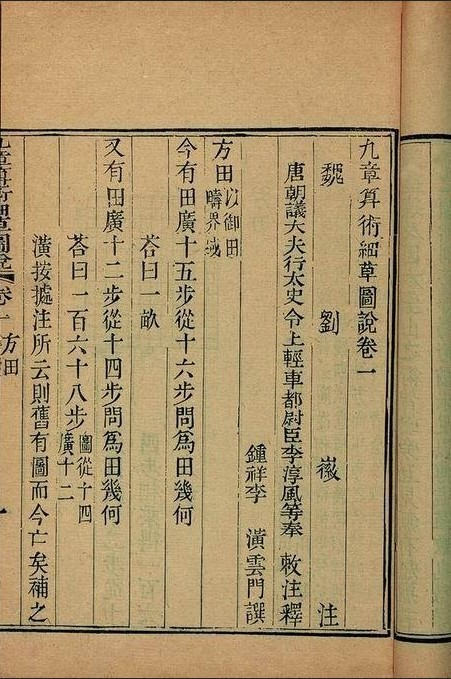
\includegraphics[width=0.4\linewidth]{image/jiuzhang.jpg}
	\caption{《九章算术》书影}
	\label{fig:jiuzhang}
	\end{figure}
	\section{线性方程组}

	形如
	\begin{equation}\label{eq:linsys}
		\left\{\begin{array}{l}
			a_{11}x_1 + a_{12}x_2 + \cdots + a_{1n}x_n = b_1,\\
			a_{21}x_1 + a_{22}x_2 + \cdots + a_{2n}x_n = b_2,\\
			\qquad\qquad\cdots\cdots\\
			a_{m1}x_1 + a_{m2}x_2 + \cdots + a_{mn}x_n = b_m
		\end{array}\right.
	\end{equation}
	的方程组称为 $m$ 个方程、$n$ 个未知量的\textbf{线性方程组}\index{xian4xing4 fang1cheng2zu3@线性方程组}，其中系数 $a_{ij}$ 与常数项 $b_i$ 都是给定的数. 若 $b_1=\cdots=b_m=0$，称之为\textbf{齐次}\index{qi2ci4 xian4xing4 fang1cheng2zu3@齐次线性方程组}线性方程组，否则称为\textbf{非齐次}\index{fei1qi2ci4 xian4xing4 fang1cheng2zu3@非齐次线性方程组}的. ``齐次''的意思是``次数整齐''：这时方程中的每一项 $a_{ij}x_j$ 都是关于未知量的一次项，次数完全一样；而非零的常数项 $b_i$ 是零次项，混在其中就``不齐''了. 一组数 $(c_1,\ldots,c_n)$ 若代入后使每个方程都成立，就称为方程组的一个\textbf{解}；全部解构成的集合称为\textbf{解集}\index{jie3ji2@解集}. 两个方程组若解集相同，则称它们\textbf{同解}\index{tong2jie3@同解}.
	
	线性方程组的解只取决于系数和常数项，与未知量用什么字母表示无关. 因此我们把它们``抽出来''排成一张表
	\[
	\left(\begin{NiceArray}{cccc:c}
		a_{11} & a_{12} & \cdots & a_{1n} & b_1\\
		a_{21} & a_{22} & \cdots & a_{2n} & b_2\\
		\vdots & \vdots &        & \vdots & \vdots\\
		a_{m1} & a_{m2} & \cdots & a_{mn} & b_m
	\end{NiceArray}\right),
	\]
	称为方程组的\textbf{增广矩阵}\index{zeng1guang3 ju3zhen4@增广矩阵}；去掉最后一列得到的表称为\textbf{系数矩阵}\index{xi4shu4 ju3zhen4@系数矩阵}. ``矩阵''的系统理论在第三章展开，本章只把它当作记录方程组的表格.
	
	\section{消元法与初等行变换}
	
	中学解方程组时，我们常做三件事：交换两个方程的位置；把某个方程两边同乘一个非零数；把某个方程的若干倍加到另一个方程上. 反映在增广矩阵上，就是下面三种操作.
	
	\begin{definition}
		以下三种操作称为矩阵的\textbf{初等行变换}\index{chu1deng3 hang2 bian4huan4@初等行变换}(elementary row operations)：
		\begin{enumerate}
			\item \textbf{对换}：交换第 $i,j$ 两行，记为 $r_i\leftrightarrow r_j$；
			\item \textbf{倍乘}：第 $i$ 行乘以非零数 $k$，记为 $kr_i$；
			\item \textbf{倍加}：把第 $j$ 行的 $c$ 倍加到第 $i$ 行上（$i\ne j$），记为 $r_i+cr_j$.
		\end{enumerate}
		若矩阵 $\vv{A}$ 经有限次初等行变换化为 $\vv{B}$，称 $\vv{A}$ 与 $\vv{B}$ \textbf{行等价}\index{hang2 deng3jia4@行等价}.
	\end{definition}
	
	\begin{theorem}\label{thm:sameSolution}
		对线性方程组的增广矩阵施行初等行变换，所得方程组与原方程组同解.
	\end{theorem}
	
	\begin{proof}
		只需对一次变换证明. 设变换前后的方程组分别为 (I) 与 (II). (I) 的任一解代入 (II) 的每个方程：对换和倍乘显然仍成立；倍加时新的第 $i$ 个方程是原第 $i$ 个方程与第 $j$ 个方程 $c$ 倍之和，两边仍相等. 故 (I) 的解都是 (II) 的解.
		
		反过来，每一种初等行变换都可以被同类变换``撤销''：$r_i\leftrightarrow r_j$ 再做一次即还原，$kr_i$ 用 $\frac1k r_i$ 还原，$r_i+cr_j$ 用 $r_i-cr_j$ 还原. 于是 (I) 也可由 (II) 经一次初等行变换得到，由刚才的论证，(II) 的解也都是 (I) 的解.
	\end{proof}
	
	\begin{motivebox}
		证明的关键不在于``变换后解还成立''，而在于``变换可以撤销''. 一个只能单向推出的变形（例如两边同乘 $0$，或两边平方）可能引入增根或丢失解. 后面我们会一再遇到这一思想：\textbf{可逆的操作保持本质，不可逆的操作会丢失信息}.
	\end{motivebox}
	
	\begin{example}\label{eg:elementarytf}
		解方程组
		\[\left\{\begin{array}{l}
			2x + 2y + z = 10, \\
			4x + 4y + 3z = 22, \\
			8x + 10y + 6z = 46.
		\end{array}\right.\]
	\end{example}
	
	\begin{solution}
		对增广矩阵施行初等行变换：
		\[
		\begin{pmatrix}
			2 & 2 & 1 & 10 \\
			4 & 4 & 3 & 22 \\
			8 & 10 & 6 & 46
		\end{pmatrix}
		\xrightarrow{\frac12 r_1}
		\begin{pmatrix}
			1 & 1 & \frac{1}{2} & 5 \\
			4 & 4 & 3 & 22 \\
			8 & 10 & 6 & 46
		\end{pmatrix}
		\xrightarrow{r_2-4r_1}
		\begin{pmatrix}
			1 & 1 & \frac{1}{2} & 5 \\
			0 & 0 & 1 & 2 \\
			8 & 10 & 6 & 46
		\end{pmatrix}.
		\]
		第二行的 $y$ 系数已经是 $0$，无法用它消去第三行的 $y$，于是交换第二、三行，再消元：
		\[
		\xrightarrow{r_2\leftrightarrow r_3}
		\begin{pmatrix}
			1 & 1 & \frac{1}{2} & 5 \\
			8 & 10 & 6 & 46 \\
			0 & 0 & 1 & 2
		\end{pmatrix}
		\xrightarrow{r_2-8r_1}
		\begin{pmatrix}
			1 & 1 & \frac{1}{2} & 5 \\
			0 & 2 & 2 & 6 \\
			0 & 0 & 1 & 2
		\end{pmatrix}
		\xrightarrow{\frac12 r_2}
		\begin{pmatrix}
			1 & 1 & \frac{1}{2} & 5 \\
			0 & 1 & 1 & 3 \\
			0 & 0 & 1 & 2
		\end{pmatrix}.
		\]
		最后一个矩阵对应的方程组可以从下往上``回代''：$z=2$，$y=3-z=1$，$x=5-y-\frac12z=3$. 由定理~\ref{thm:sameSolution}，原方程组有唯一解 $(x,y,z)=(3,1,2)$.
	\end{solution}
	
	\section{阶梯形矩阵}
	
	例~\ref{eg:elementarytf} 的最后一个矩阵有一种``台阶''形状. 我们把它一般化.
	
	\begin{definition}
		称矩阵某一行从左数第一个非零元为该行的\textbf{主元}\index{zhu3yuan2@主元}. 若矩阵满足
		\begin{enumerate}
			\item 全零行（如果有）都在非零行的下方；
			\item 每个非零行的主元，都严格位于上一行主元的右侧，
		\end{enumerate}
		则称它为\textbf{阶梯形矩阵}\index{jie1ti1xing2 ju3zhen4@阶梯形矩阵}. 若阶梯形矩阵还满足：每个主元都是 $1$，且主元所在列的其他元素都是 $0$，则称它为\textbf{简化阶梯形矩阵}\index{jian3hua4 jie1ti1xing2 ju3zhen4@简化阶梯形矩阵}.
	\end{definition}
	
	\begin{theorem}\label{thm:rref}
		任何矩阵都可以经有限次初等行变换化为简化阶梯形.
	\end{theorem}
	
	\begin{proof}
		对列数归纳，给出一个算法. 找到最左边的不全为零的列，用对换把该列的一个非零元换到第一行，再用倍乘把它变为 $1$，用倍加把该列其余元素消为 $0$. 此后第一行固定不动，对剩下的行（它们在这一列及左边全为 $0$）重复同样的过程. 每一步使处理过的列数增加，有限步后得到阶梯形. 最后从最下面一个主元开始，用倍加把每个主元上方的元素消为零，即得简化阶梯形.
	\end{proof}
	
	\begin{remark}
		一个矩阵的简化阶梯形是唯一的（见第一章章末习题~\ref{ex:elim:C9}）. 但阶梯形不唯一，例如再做一次倍乘仍是阶梯形.
	\end{remark}
	\begin{figure}[htbp]
		\centering
		\begin{tikzpicture}[x=0.75cm,y=0.6cm]
			\foreach \row [count=\i] in {
				{{\color{figred}\blacksquare},*,*,*,*,*},
				{{\color{gray}0},{\color{gray}0},{\color{figred}\blacksquare},*,*,*},
				{{\color{gray}0},{\color{gray}0},{\color{gray}0},{\color{figred}\blacksquare},*,*},
				{{\color{gray}0},{\color{gray}0},{\color{gray}0},{\color{gray}0},{\color{gray}0},{\color{gray}0}}}{
				\foreach \e [count=\j] in \row {
					\node at (\j-0.5,-\i+0.5) {$\e$};
				}
			}
			\draw[figred,thick] (0,-1) -- (2,-1) -- (2,-2) -- (3,-2) -- (3,-3) -- (6,-3);
			\draw[thick] (0.1,0.1) -- (-0.1,0.1) -- (-0.1,-4.1) -- (0.1,-4.1);
			\draw[thick] (5.9,0.1) -- (6.1,0.1) -- (6.1,-4.1) -- (5.9,-4.1);
			\node[right,font=\small,align=left] at (6.6,-1.2) {{\color{figred}$\blacksquare$}：主元（非零）\\ $*$：任意数};
		\end{tikzpicture}
		\caption{阶梯形矩阵. 红线以下全为零，每个主元都在上一行主元的右侧，像一级级台阶.}
		\label{fig:echelon}
	\end{figure}
	\section{解的判定}
	
	设方程组~\eqref{eq:linsys} 的增广矩阵已化为简化阶梯形. 主元所在列对应的未知量称为\textbf{主变量}\index{zhu3 bian4liang4@主变量}，其余未知量称为\textbf{自由变量}\index{zi4you2 bian4liang4@自由变量}.
	
	\begin{theorem}\label{thm:solvability}
		设方程组~\eqref{eq:linsys} 的增广矩阵行等价于简化阶梯形 $\vv{R}$，$\vv{R}$ 中位于系数部分的主元有 $r$ 个. 则
		\begin{enumerate}
			\item 方程组有解，当且仅当 $\vv{R}$ 中没有形如 $(0,\ldots,0\mid d)$（$d\ne0$）的行；
			\item 有解时，若 $r=n$，则解唯一；若 $r<n$，则有 $n-r$ 个自由变量，它们可以任意取值，解有无穷多个.
		\end{enumerate}
	\end{theorem}
	
	\begin{proof}
		若有形如 $(0,\ldots,0\mid d)$（$d\ne 0$）的行，它对应方程 $0=d$，无解. 否则，$\vv{R}$ 的每个非零行都形如``某主变量 $+$ 若干自由变量的线性组合 $=$ 常数''，且每个主变量只出现在一个方程中. 任意给定自由变量的值，主变量的值就被唯一确定，这样得到的全部数组恰好就是解集. 没有自由变量（$r=n$）时解唯一；有自由变量时，不同的取值给出不同的解.
	\end{proof}
	\begin{figure}[htbp]
		\centering
		\begin{tikzpicture}[scale=0.85]
			\foreach \dx/\lab in {0/{(a) 相交：唯一解}, 4.2/{(b) 平行：无解}, 8.4/{(c) 重合：无穷多解}}{
				\begin{scope}[xshift=\dx cm]
					\draw[axis] (-0.3,0) -- (3,0);
					\draw[axis] (0,-0.3) -- (0,2.4);
					\node[sub] at (1.35,-0.75) {\lab};
				\end{scope}
			}
			\draw[thick,figblue] (0.1,0.2) -- (2.7,2.0);
			\draw[thick,figorange] (0.1,2.0) -- (2.7,0.4);
			\node[dot,figred] at (1.48,1.155) {};
			\begin{scope}[xshift=4.2cm]
				\draw[thick,figblue] (0.1,0.3) -- (2.7,1.6);
				\draw[thick,figorange] (0.1,0.9) -- (2.7,2.2);
			\end{scope}
			\begin{scope}[xshift=8.4cm]
				\draw[line width=3pt,figorange!50] (0.1,0.3) -- (2.7,2.0);
				\draw[thick,figblue] (0.1,0.3) -- (2.7,2.0);
			\end{scope}
		\end{tikzpicture}
		\caption{两个未知量、两个方程：每个方程是平面上的一条直线，解是它们的公共点.}
		\label{fig:twolines}
	\end{figure}
	
	\begin{corollary}\label{cor:homogeneous}
		齐次线性方程组若方程个数少于未知量个数（$m<n$），则必有非零解.
	\end{corollary}
	
	\begin{proof}
		齐次方程组总有零解，所以有解. 主元个数 $r\le m<n$，故至少有一个自由变量，令它取 $1$ 就得到一个非零解.
	\end{proof}
	
	\begin{motivebox}
		这个推论看起来朴素，第二章``维数''理论中的许多结论却都以它为依据：基本引理的证明直接用到它，而``任意两组基所含向量个数相同''又由基本引理推出. 请记住它：\textbf{未知量比方程多，齐次方程组就有非零解.}
	\end{motivebox}
	
	\begin{example}
		解方程组
		\[\left\{\begin{array}{l}
			x_1+2x_2-x_3+x_4=1,\\
			2x_1+4x_2-x_3+3x_4=4,\\
			x_1+2x_2+x_3+3x_4=5.
		\end{array}\right.\]
	\end{example}
	
	\begin{solution}
		\[
		\begin{pmatrix}
			1&2&-1&1&1\\ 2&4&-1&3&4\\ 1&2&1&3&5
		\end{pmatrix}
		\xrightarrow[r_3-r_1]{r_2-2r_1}
		\begin{pmatrix}
			1&2&-1&1&1\\ 0&0&1&1&2\\ 0&0&2&2&4
		\end{pmatrix}
		\xrightarrow[r_1+r_2]{r_3-2r_2}
		\begin{pmatrix}
			1&2&0&2&3\\ 0&0&1&1&2\\ 0&0&0&0&0
		\end{pmatrix}.
		\]
		主变量为 $x_1,x_3$，自由变量为 $x_2,x_4$. 令 $x_2=s$，$x_4=t$，得全部解
		\[
		x_1=3-2s-2t,\quad x_2=s,\quad x_3=2-t,\quad x_4=t\qquad(s,t\ \text{任意}).
		\]
		若把第三个方程的常数项 $5$ 改为 $6$，同样的变换会得到一行 $(0,0,0,0\mid 1)$，方程组无解.
	\end{solution}
	
	\begin{linkbox}{投入产出模型}\index{tou2ru4 chan3chu1 mo2xing2@投入产出模型}
		设某经济体只有农业、制造业两个部门. 每生产 $1$ 单位农产品需要消耗 $0.2$ 单位农产品和 $0.4$ 单位工业品；每生产 $1$ 单位工业品需要消耗 $0.3$ 单位农产品和 $0.1$ 单位工业品. 若社会最终需求为农产品 $110$ 单位、工业品 $170$ 单位，两部门各应生产多少？
		
		设总产出为 $x_1,x_2$. 总产出 $=$ 中间消耗 $+$ 最终需求，即
		\[
		x_1=0.2x_1+0.3x_2+110,\qquad x_2=0.4x_1+0.1x_2+170.
		\]
		整理后是一个线性方程组，消元得 $x_1=250$，$x_2=300$. 
		
		这类模型由列昂惕夫（W.~Leontief）系统发展，他因此获得 1973 年诺贝尔经济学奖. 真实的投入产出表有上百个部门，方程组的规模随之变大，但解法正是本章的消元法. 第三章我们会把它写成 $(\vv{I}-\vv{A})\vv{x}=\vv{d}$ 的矩阵形式.
	\end{linkbox}
	\begin{modelbox}{物流网络的流量平衡}
		\mstep{问题} 某公司每天从仓库 $A$ 向门店 $D$ 运送 $50$ 吨货物，途经中转站 $B,C$. 可用线路为 $A\to B$，$A\to C$，$B\to C$，$B\to D$，$C\to D$，流量依次记为 $x_1,\ldots,x_5$. 流量应当怎样安排？
		\begin{center}
			\begin{tikzpicture}
				\node[station] (A) at (0,0) {$A$};
				\node[station] (B) at (2.6,1.3) {$B$};
				\node[station] (C) at (2.6,-1.3) {$C$};
				\node[station] (D) at (5.2,0) {$D$};
				\draw[vec,figblue] (A) -- node[above left]{$x_1$} (B);
				\draw[vec,figblue] (A) -- node[below left]{$x_2$} (C);
				\draw[vec,figblue] (B) -- node[right]{$x_3$} (C);
				\draw[vec,figblue] (B) -- node[above right]{$x_4$} (D);
				\draw[vec,figblue] (C) -- node[below right]{$x_5$} (D);
				\draw[vec,figorange] (-1.5,0) node[left,font=\small]{供给 $50$} -- (A);
				\draw[vec,figorange] (D) -- (6.7,0) node[right,font=\small]{需求 $50$};
			\end{tikzpicture}
			\captionof{figure}{物流网络. 箭头是线路方向，$x_i$ 是每天的流量（吨）.}
			\label{fig:logistics}
		\end{center}
		\mstep{假设} 中转站不囤货（流入 $=$ 流出）；途中没有损耗.
		
		\mstep{模型} 对每个站点写``流出 $-$ 流入 $=$ 净供给''：
		\[\left\{\begin{array}{rcl}
			x_1+x_2&=&50 \quad (A),\\
			-x_1+x_3+x_4&=&0 \quad (B),\\
			-x_2-x_3+x_5&=&0 \quad (C),\\
			-x_4-x_5&=&-50 \quad (D).
		\end{array}\right.\]
		
		\mstep{求解} 消元后系数部分只有 $3$ 个主元：四个方程相加得 $0=0$，其中一个是多余的. 取 $x_3=s$，$x_4=t$ 为自由变量，得
		\[x_1=s+t,\quad x_2=50-s-t,\quad x_3=s,\quad x_4=t,\quad x_5=50-t.\]
		
		\mstep{解读}
		\begin{itemize}
			\item 多余的方程反映了一个守恒律：\textbf{总供给 $=$ 总需求}. 若把 $D$ 的需求改为 $40$，方程组立刻无解——定理~\ref{thm:solvability} 替我们发现了``账不平''.
			\item 两个自由变量是调度员手中的两个``旋钮''：$s$ 每增加 $1$，就有 $1$ 吨货从``$A\to C$ 直达''改为``$A\to B\to C$ 绕行''；$t$ 每增加 $1$，就有 $1$ 吨货从``$A\to C\to D$''改走``$A\to B\to D$''.
			\item 方程组只告诉我们\textbf{哪些方案可行}，不告诉我们\textbf{选哪个}. 选择需要额外的目标，比如运费最低.
		\end{itemize}
		
		\mstep{局限} 现实中流量不能为负（$s,t\ge0$，$s+t\le50$），线路还有容量上限. 加上这些不等式约束和成本目标，问题就成了\textbf{线性规划}\index{xian4xing4 gui1hua4@线性规划}，属于运筹学. 线性代数提供的是它的骨架：可行方案集正是上面这个``双参数''解集的一部分. 第六章还会回到这个例子.
	\end{modelbox}
	
	\begin{historybox}{方程术}

		西方把消元法冠以高斯之名，但成书于公元 1 世纪前后的《九章算术》``方程''章已经把方程组的系数排成算筹方阵，用``遍乘''与``直除''（即倍乘与倍加）逐列消元\cite{guo2004jiuzhang,shen1999nine}. 中文``方程''一词的本义，正是这种``并而列之''的方阵.
	\end{historybox}
	
	\begin{codebox}{消元法的算法实现}
		\mstep{目标} 把本章的消元法写成一个程序，再用它重新``读''一遍物流网络.
		
		\mstep{准备} Python 的 \texttt{fractions.Fraction}（精确分数，避免小数带来的舍入误差）；用于对照的 \texttt{sympy} 中的 \texttt{Matrix(M).rref()}；\texttt{numpy.linalg.solve}.
		
		\mstep{任务}
		\begin{enumerate}
			\item 按定理~\ref{thm:rref} 证明中给出的算法，写函数 \texttt{rref(M)}：输入一个用列表表示的矩阵，返回它的简化阶梯形以及主元所在的列号. 全程用 \texttt{Fraction} 运算.
			\item 用例~\ref{eg:elementarytf} 的增广矩阵检验你的函数，并与 \texttt{sympy} 的结果比较.
			\item 输入物流网络的 $4\times6$ 增广矩阵（未知量依次为 $x_1,\ldots,x_5$），求简化阶梯形，写出主元列与自由变量，并据此写出全部解.
			\item 把 $D$ 的需求从 $50$ 改为 $40$，再算一次，指出是哪一行说明了方程组无解.
			\item 用 \texttt{numpy.linalg.solve} 去解物流网络，记录它的报错信息.
		\end{enumerate}
		
		\mstep{检查点} 例~\ref{eg:elementarytf} 的解为 $(3,1,2)$；物流网络的系数部分有 $3$ 个主元；需求改为 $40$ 后，简化阶梯形的最后一行是 $(0,0,0,0,0\mid1)$.
		
		\mstep{思考}
		\begin{enumerate}
			\item 你的程序选出的自由变量是什么？正文选的是 $x_3,x_4$. 两种写法给出的是同一个解集吗？请用计算验证，并说明为什么``选哪几个当自由变量''不是唯一的.
			\item \texttt{solve} 为什么拒绝解物流网络？它只能处理哪一类方程组？这对``出错了就换个函数试试''的习惯有什么提醒？
		\end{enumerate}
	\end{codebox}
	
	\ExElimination
	
	% =====================================================================
	\chapter{向量空间}\label{ch:vectorspace}
	
	\paragraph*{本章地位}
	
	第一章给出了求解方程组的方法，但没有回答解集具有怎样的结构. 要回答这一问题，需要把一组数作为整体来研究. 本章从数域出发，用八条运算律定义向量空间，并建立线性相关、秩、子空间、基与维数等概念. 这套语言是全书的基础，此后关于矩阵、方程组和线性映射的讨论都在它之上展开. 本章最后证明，同一数域上维数相同的有限维向量空间都同构于 $\mathbb{F}^n$.
	
	\chapterhours{6}{7}{9}
	
	\begin{introduction}[学习目标]
		\item 验证一个集合关于给定的运算是否构成数域、向量空间或子空间
		\item 判断向量组的线性相关性，求向量组的秩与一个极大无关组
		\item 说明极大无关组所含向量的个数为什么与选取方式无关
		\item 求向量空间或子空间的基与维数，把线性无关组扩充为基
		\item 求向量在给定基下的坐标，说明有限维向量空间与 $\mathbb{F}^n$ 同构
		\item \hC 覆盖定理的叙述与证明
		\item \hC 空间的直和与直和分解
	\end{introduction}
	
	\paragraph*{前置知识}
	
	第一章（消元法与齐次方程组的解）；中学的平面向量与空间向量.
	
	\paragraph*{学习提示}
	\begin{itemize}
		\item 本章是全书从具体走向抽象的第一步. 向量空间由运算规则定义，而不由元素的具体形态定义. 遇到抽象概念时，应在数组、多项式、函数等具体空间中加以检验.
		\item 本章关于``个数''的结论，包括秩、维数与基所含向量的个数，都依赖于基本引理，而基本引理又依赖于第一章关于齐次方程组的结论. 理清这一推理顺序，就把握了本章的结构.
		\item 极大无关组、基、维数与秩是从不同角度描述同一个量：一个向量组或一个空间中线性无关的向量最多有几个. 学完本章后，应能说明它们之间的关系.
	\end{itemize}
	
	\newpage
	
	\begin{tcolorbox}[epigraph, epigraph image*={0.25\linewidth}{image/poincare.jpg}{亨利·庞加莱}{fig:poincare}]
		\begin{quote}\textit{La mathématique est l'art de donner le même nom à des choses différentes.}\end{quote}
		\begin{flushright}——Henri Poincaré, \textit{Science et méthode}\end{flushright}
		\begin{quote}数学是给不同的东西以相同名称的艺术.\end{quote}
		\begin{flushright}——亨利·庞加莱\footnotemark\end{flushright}
	\end{tcolorbox}
	\footnotetext{亨利·庞加莱（1854—1912），法国数学家、物理学家、科学哲学家，在微分方程、天体力学、拓扑学等领域有奠基性贡献. 这句话出自其科学哲学著作《科学与方法》（1908）.}
	
	\section{数域}
	
	中学里，``代数''几乎就是``解方程''：用字母表示未知的数，按规则变形，直到求出它. 不妨回头看看，这些变形依靠的究竟是什么. 解 $3x+2=8$ 时，我们两边减去 $2$，再两边除以 $3$. 这里用到的，是``可以做减法''``可以除以非零数''这样的\textbf{运算规则}，而不是 $3$、$2$、$8$ 这几个数本身. 换一批数，只要同样的运算能做、同样的规则成立，解法就原封不动；反过来，若只允许使用整数，$3x=2$ 就无解了——缺的不是某个数，而是``除法''这条规则.
	
	这提示我们换一个角度看代数学：与其盯着具体的数，不如研究运算本身，以及运算所遵守的规则. 一个集合，配上若干种运算，运算满足一定的规则，就称为一个\textbf{代数结构}. 代数学研究的，是代数结构以及它们之间的关系. 本书从最简单的一种代数结构开始：能自由地做四则运算的数集.
	
	\begin{definition}
		设 $\mathbb{F}$ 是复数集的子集，且至少含有两个不同的元素. 若 $\mathbb{F}$ 中任意两个数的和、差、积、商（除数不为零）仍在 $\mathbb{F}$ 中，就称 $\mathbb{F}$ 是一个\textbf{数域}\index{shu4yu4@数域}(number field).
	\end{definition}
	
	有理数集 $\mathbb{Q}$、实数集 $\mathbb{R}$、复数集 $\mathbb{C}$ 都是数域. 整数集 $\mathbb{Z}$ 不是数域，因为 $1\div 2\notin\mathbb{Z}$.
	
	\begin{example}
		证明：$\mathbb{Q}(\sqrt{2}) = \{ a+b\sqrt{2} \mid a,b \in \mathbb{Q} \}$ 是数域.
	\end{example}
	\begin{proof}
		和、差、积仍为 $a+b\sqrt2$ 型是直接验证的. 对于商，设 $c+d\sqrt{2}\ne 0$（$c,d\in\mathbb{Q}$）. 先说明 $c-d\sqrt2\neq 0$：否则 $c=d\sqrt2$，若 $d\ne0$ 则 $\sqrt2=c/d$ 是有理数，矛盾；若 $d=0$ 则 $c=0$，与 $c+d\sqrt2\ne0$ 矛盾. 于是可以分母有理化：
		\[
		\frac{a+b\sqrt{2}}{c+d\sqrt{2}}=\frac{(a+b\sqrt{2})(c-d\sqrt{2})}{c^2-2d^2}=\frac{ac-2bd}{c^2-2d^2}+\frac{bc-ad}{c^2-2d^2}\sqrt{2}\in\mathbb{Q}(\sqrt2).
		\]
	\end{proof}
	
	\begin{note}
		任何数学定义提出之后，都应当\textbf{验证满足定义的对象确实存在}. 研究一个空洞的概念是没有意义的——在数理逻辑中，从矛盾的前提可以推出任何结论. 
		
		举一个例子. 设 $N$ 是最大的正整数. 由于 $N^2$ 也是正整数，而 $N$ 最大，故 $N^2\le N$；又 $N\ge1$，故 $N^2\ge N$. 于是 $N^2=N$，得 $N=1$——``最大的正整数是 $1$''. 推理的每一步都无懈可击，错在第一句：最大的正整数根本不存在.
	\end{note}
	
	\begin{theorem}\label{thm:Qsmallest}
		任何数域都包含有理数域. 即有理数域是最小的数域.
	\end{theorem}
	\begin{proof}
		设 $\mathbb{F}$ 是数域. 由于 $\mathbb{F}$ 至少有两个不同元素，其中必有非零数 $a$. 于是 $1=a\div a\in\mathbb{F}$，$0=a-a\in\mathbb{F}$. 由 $1$ 反复相加、相减得到全部整数，再作商得到全部有理数 $m/n$（$n\ne0$）. 故 $\mathbb{Q}\subset\mathbb{F}$.
	\end{proof}
	
	\begin{exercise}
		\begin{enumerate}
			\item 证明：$\{a+b\sqrt[3]{2}+c\sqrt[3]{4}\mid a,b,c\in\mathbb{Q}\}$ 是数域.（提示：除法是难点，可先证明非零元都有逆元.）
			\item $\{a+b\mathrm{i}\mid a,b\in\mathbb{Q}\}$ 是否是数域？$\{a+b\sqrt2\mid a,b\in\mathbb{Z}\}$ 呢？
			\item 证明：若 $\mathbb{F}_1,\mathbb{F}_2$ 是数域，则 $\mathbb{F}_1\cap\mathbb{F}_2$ 也是数域.
		\end{enumerate}
	\end{exercise}
	
	\section{\texorpdfstring{$n$}{n} 维向量}
	
	\begin{definition}\label{def:vec}
		数域 $\mathbb{F}$ 中的 $n$ 个数 $a_1,a_2,\ldots,a_n$ 排成的有序数组
		\[\vv{\alpha}=\begin{pmatrix} a_1 \\ a_2 \\ \vdots \\ a_n \end{pmatrix}\]
		称为 $\mathbb{F}$ 上的 $n$ 维\textbf{列向量}\index{lie4 xiang4liang4@列向量}，$a_i$ 称为它的第 $i$ 个分量. 排成一行的 $(a_1,a_2,\ldots,a_n)$ 称为 $n$ 维\textbf{行向量}\index{hang2 xiang4liang4@行向量}. 全体 $n$ 维列向量的集合记为 $\mathbb{F}^n$.
	\end{definition}
	
	\begin{pitfallbox}
		\begin{enumerate}
			\item 本书默认``向量''指列向量. 行向量与列向量即使分量对应相等，也是\textbf{不同}的对象，不能画等号. 列向量 $\vv\alpha$ 的转置 $\vv\alpha^\trans$ 才是对应的行向量.
			\item 两个向量相等，当且仅当维数相同且分量按顺序对应相等. 因此 $(1,2,0)^\trans\ne(1,2)^\trans$：多出来的分量即使是 $0$ 也不能忽略.
			\item 不同维数的向量之间不定义加法.
		\end{enumerate}
	\end{pitfallbox}
	
	对 $k\in\mathbb{F}$ 和 $\vv{\alpha}=(a_1,\ldots,a_n)^\trans$，$\vv{\beta}=(b_1,\ldots,b_n)^\trans$，定义
	\[
	\vv{\alpha} + \vv{\beta} = \begin{pmatrix} a_1+ b_1 \\ \vdots \\ a_n+ b_n \end{pmatrix},\qquad
	k \vv{\alpha} = \begin{pmatrix} ka_1 \\ \vdots \\ ka_n \end{pmatrix}.
	\]
	加法与数乘统称为\textbf{线性运算}\index{xian4xing4 yun4suan4@线性运算}. 分量全为 $0$ 的向量称为\textbf{零向量}\index{ling2 xiang4liang4@零向量}，记为 $\zero$；$-\vv\alpha=(-1)\vv\alpha$ 称为 $\vv\alpha$ 的\textbf{负向量}，并规定 $\vv\alpha-\vv\beta=\vv\alpha+(-\vv\beta)$. 容易逐个分量验证，对任意 $\vv\alpha,\vv\beta,\vv\gamma\in\mathbb{F}^n$ 与 $k,l\in\mathbb{F}$：
	\begin{enumerate}
		\item $\vv{\alpha}+\vv{\beta} =\vv{\beta}+\vv{\alpha}$；
		\item $(\vv{\alpha}+\vv{\beta})+\vv{\gamma} = \vv{\alpha}+(\vv{\beta}+\vv{\gamma})$；
		\item $\vv{\alpha}+\zero=\vv{\alpha}$；
		\item $\vv{\alpha}+(-\vv{\alpha})=\zero$；
		\item $1\vv{\alpha}=\vv{\alpha}$；
		\item $(kl)\vv{\alpha}=k(l\vv{\alpha})$；
		\item $k(\vv{\alpha}+\vv{\beta})=k\vv{\alpha}+k\vv{\beta}$；
		\item $(k+l)\vv{\alpha}=k\vv{\alpha}+l\vv{\alpha}$.
	\end{enumerate}
	\begin{figure}[htbp]
		\centering
		\begin{tikzpicture}[
			subcap/.style={sub,anchor=north,text width=4.3cm,align=center}]
			\begin{scope}
				\draw[axis] (-0.3,0) -- (3.2,0);
				\draw[axis] (0,-0.3) -- (0,2.6);
				\coordinate (a) at (2.2,0.5); \coordinate (b) at (0.7,1.7);
				\draw[dashed,gray] (a) -- ($(a)+(b)$) -- (b);
				\draw[vec,figblue] (0,0) -- (a) node[below right]{$\vv\alpha$};
				\draw[vec,figorange] (0,0) -- (b) node[left]{$\vv\beta$};
				\draw[vec,figred] (0,0) -- ($(a)+(b)$) node[above right]{$\vv\alpha+\vv\beta$};
				\node[subcap] at (1.45,-1.1) {(a) 加法：平行四边形法则};
			\end{scope}
			\begin{scope}[xshift=5.6cm]
				\draw[axis] (-1.6,0) -- (3.2,0);
				\draw[axis] (0,-0.9) -- (0,2.6);
				\draw[gray!40] (-1.5,-0.6) -- (3.2,1.28);
				\draw[vec,figblue,line width=2.4pt,opacity=0.35] (0,0) -- (3,1.2);
				\node[figblue,above] at (2.9,1.2) {$1.5\vv\alpha$};
				\draw[vec,figblue] (0,0) -- (2,0.8) node[above,pos=0.6]{$\vv\alpha$};
				\draw[vec,figred] (0,0) -- (-1.2,-0.48) node[above left]{$-\vv\alpha$};
				\node[subcap] at (0.8,-1.1) {(b) 数乘：沿同一直线伸缩、反向};
			\end{scope}
		\end{tikzpicture}
		\caption{平面向量的线性运算.}
		\label{fig:vecops}
	\end{figure}
	\section{向量空间}
	
	研究函数时，我们关心的往往是一类函数共同的性质；研究向量也是如此. 上面八条运算律并不依赖``向量是一列数''这件事——许多别的对象也满足它们. 于是我们把这八条规则本身作为定义.
	
	\begin{definition}
		设 $\mathbb{F}$ 是数域，$V$ 是非空集合. 若在 $V$ 上定义了
		\begin{itemize}
			\item \textbf{加法}：对任意 $\vv{\alpha}, \vv{\beta} \in V$，有唯一的 $\vv{\alpha} + \vv{\beta} \in V$；
			\item \textbf{数乘}：对任意 $k \in \mathbb{F}$ 和 $\vv{\alpha} \in V$，有唯一的 $k \vv{\alpha} \in V$，
		\end{itemize}
		且它们满足上一节列出的八条运算律（其中第 3、4 条理解为：\textbf{存在}某个元素 $\zero\in V$ 使第 3 条对一切 $\vv\alpha$ 成立；对每个 $\vv\alpha$ \textbf{存在}某个 $-\vv\alpha\in V$ 使第 4 条成立），则称 $V$ 是数域 $\mathbb{F}$ 上的\textbf{向量空间}\index{xiang4liang4 kong1jian1@向量空间}(vector space)，也称\textbf{线性空间}\index{xian4xing4 kong1jian1@线性空间}. $V$ 中的元素称为向量.
	\end{definition}
	
	这个定义冗长但好理解：向量空间就是一个配备了两种运算、遵守八条规则的集合. 下面的例子说明，许多看似无关的对象都是向量空间.
	
	\begin{example}
		$\mathbb{F}^n$ 关于上一节的运算是 $\mathbb{F}$ 上的向量空间. 特别地有 $\mathbb{R}^n$.
	\end{example}
	
	\begin{example}
		系数属于 $\mathbb{F}$ 的一元多项式全体 $\mathbb{F}[x]$，关于多项式的加法和数乘构成向量空间. 次数小于 $n$ 的多项式（含零多项式）全体 $\mathbb{F}[x]_n$ 也构成向量空间.
	\end{example}
	
	\begin{example}
		复数集 $\mathbb{C}$ 关于复数加法和``实数乘复数''构成 $\mathbb{R}$ 上的向量空间.
	\end{example}
	
	\begin{example}
		闭区间 $[a,b]$ 上的实值连续函数全体 $C[a,b]$，关于 $(f+g)(x)=f(x)+g(x)$，$(kf)(x)=kf(x)$ 构成 $\mathbb{R}$ 上的向量空间.
	\end{example}
	
	\begin{linkbox}{价格与数量}
		一家超市销售 $n$ 种商品. 一张购物清单是一个 $n$ 维向量（各商品的购买数量），一张价目表也是一个 $n$ 维向量. 两张清单合并就是向量相加，``全部翻倍''就是数乘. 经济学中的``商品空间''正是 $\mathbb{R}^n$.
	\end{linkbox}
	
	下面推导向量空间的基本性质. 注意：我们\textbf{只能使用八条公理}，而不能使用``分量''之类的具体结构——这正是公理化方法的训练.
	
	\begin{theorem}
		向量空间中的零向量是唯一的；每个向量的负向量也是唯一的.
	\end{theorem}
	\begin{proof}
		设 $\zero_1,\zero_2$ 都是零向量，则 $\zero_1=\zero_1+\zero_2=\zero_2+\zero_1=\zero_2$.
		
		设 $\vv\beta,\vv\gamma$ 都是 $\vv\alpha$ 的负向量，则
		$\vv\beta=\vv\beta+\zero=\vv\beta+(\vv\alpha+\vv\gamma)=(\vv\beta+\vv\alpha)+\vv\gamma=\zero+\vv\gamma=\vv\gamma.$
	\end{proof}
	
	\begin{proposition}\label{prop:linspc}
		设 $V$ 是 $\mathbb{F}$ 上的向量空间，$k\in\mathbb{F}$，$\vv{\alpha},\vv{\beta},\vv{\gamma}\in V$，则
		\begin{enumerate}
			\item （消去律）若 $\vv{\alpha}+\vv{\beta}=\vv{\alpha}+\vv{\gamma}$，则 $\vv{\beta}=\vv{\gamma}$；
			\item $0\vv{\alpha}=\zero$；
			\item $k\zero=\zero$；
			\item $(-1)\vv{\alpha}=-\vv{\alpha}$；
			\item 若 $k\vv{\alpha}=\zero$，则 $k=0$ 或 $\vv{\alpha}=\zero$.
		\end{enumerate}
	\end{proposition}
	\begin{proof}
		(1) 两边加上 $-\vv\alpha$ 并用结合律. (2) $0\vv\alpha=(0+0)\vv\alpha=0\vv\alpha+0\vv\alpha$，由 (1) 得 $0\vv\alpha=\zero$. (3) 同理. (4) $\vv\alpha+(-1)\vv\alpha=(1+(-1))\vv\alpha=0\vv\alpha=\zero$，由负向量唯一性得证. (5) 若 $k\ne0$，则 $\vv\alpha=1\vv\alpha=(k^{-1}k)\vv\alpha=k^{-1}(k\vv\alpha)=k^{-1}\zero=\zero$.
	\end{proof}
	
	\begin{exercise}
		\begin{enumerate}
			\item 以 $0$ 为极限的实数列全体 $V$，按 $\{a_n\}+\{b_n\}=\{a_n+b_n\}$，$k\{a_n\}=\{ka_n\}$ 定义运算，证明 $V$ 是 $\mathbb{R}$ 上的向量空间.
			\item 在正实数集 $\mathbb{R}^+$ 上定义``加法''$a\oplus b=ab$、``数乘''$k\circ a=a^k$（$k\in\mathbb{R}$）. 证明 $\mathbb{R}^+$ 是 $\mathbb{R}$ 上的向量空间，并指出它的``零向量''是什么.
			\item 在 $\mathbb{R}^2$ 上保留通常加法，定义数乘为 $k\circ(a,b)^\trans=(ka,0)^\trans$. 八条公理中哪一条不成立？
		\end{enumerate}
	\end{exercise}
	
	\section{线性相关性}
	
	\subsection{线性组合与线性相关}
	
	\begin{definition}
		设 $\vv\alpha_1,\ldots,\vv\alpha_s\in V$（称为一个\textbf{向量组}\index{xiang4liang4zu3@向量组}），$k_1,\ldots,k_s\in\mathbb{F}$，称
		\[k_1\vv\alpha_1+k_2\vv\alpha_2+\cdots+k_s\vv\alpha_s\]
		为它们的一个\textbf{线性组合}\index{xian4xing4 zu3he2@线性组合}. 若 $\vv\beta$ 等于某个线性组合，称 $\vv\beta$ 可由 $\vv\alpha_1,\ldots,\vv\alpha_s$ \textbf{线性表出}\index{xian4xing4 biao3chu1@线性表出}. 全部线性组合构成的集合称为它们的\textbf{张成}\index{zhang1cheng2@张成}(span)，记为 $\spn(\vv\alpha_1,\ldots,\vv\alpha_s)$. 约定空向量组的张成为 $\{\zero\}$.
	\end{definition}
	
	\begin{pitfallbox}
		线性组合的系数\textbf{可以全为零}. 因此零向量可由任何向量组线性表出. ``系数不全为零''的要求只出现在下面线性相关的定义中，不要把两者混淆.
	\end{pitfallbox}
	
	\begin{definition}
		若存在\textbf{不全为零}的 $k_1,\ldots,k_s\in\mathbb{F}$，使
		\[k_1\vv{\alpha}_1+k_2\vv{\alpha}_2+\cdots+k_s\vv{\alpha}_s=\zero,\]
		则称向量组 $\vv\alpha_1,\ldots,\vv\alpha_s$ \textbf{线性相关}\index{xian4xing4 xiang1guan1@线性相关}(linearly dependent)；否则，即上式只有在 $k_1=\cdots=k_s=0$ 时成立，称之\textbf{线性无关}\index{xian4xing4 wu2guan1@线性无关}(linearly independent).
	\end{definition}
	
	\begin{motivebox}
		为什么这样定义``相关''？在平面上，$\vv\alpha=\lambda\vv\beta+(1-\lambda)\vv\gamma$ 表示 $\vv\alpha$ 落在 $\vv\beta,\vv\gamma$ 终点的连线上——三个向量之间有``冗余''. 线性相关就是这种冗余的一般说法：组里至少有一个向量是多余的，见定理~\ref{thm:relvandexp}. 而用``组合为零''来表述，好处是对称——不必事先指定哪一个向量多余.
	\end{motivebox}
	\begin{figure}[htbp]
		\centering
		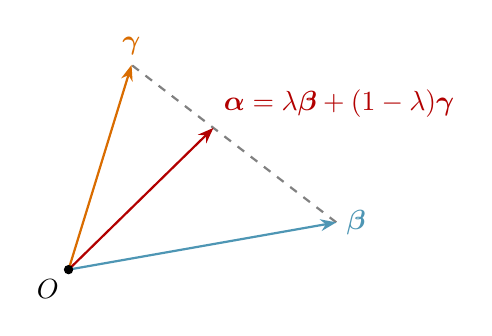
\begin{tikzpicture}
			\coordinate (O) at (0,0);
			\coordinate (b) at (3.4,0.6);
			\coordinate (c) at (0.8,2.6);
			\coordinate (a) at ($(b)!0.6!(c)$);
			\draw[dashed,gray,thick] (b) -- (c);
			\draw[vec,figblue] (O) -- (b) node[right]{$\vv\beta$};
			\draw[vec,figorange] (O) -- (c) node[above]{$\vv\gamma$};
			\draw[vec,figred] (O) -- (a) node[above right]{$\vv\alpha=\lambda\vv\beta+(1-\lambda)\vv\gamma$};
			\node[dot] at (O) {};
			\node[below left] at (O) {$O$};
		\end{tikzpicture}
		\caption{$\vv\alpha$ 的终点落在 $\vv\beta,\vv\gamma$ 终点的连线上：三个向量之间有``冗余''，它们线性相关.}
		\label{fig:lindep}
	\end{figure}
	\begin{example}
		$\mathbb{F}^n$ 中的\textbf{标准单位向量}\index{biao1zhun3 dan1wei4 xiang4liang4@标准单位向量} $\vv{e}_1,\ldots,\vv{e}_n$（$\vv e_i$ 的第 $i$ 个分量为 $1$，其余为 $0$）线性无关：$k_1\vv e_1+\cdots+k_n\vv e_n=(k_1,\ldots,k_n)^\trans=\zero$ 迫使每个 $k_i=0$.
	\end{example}
	
	\begin{example}\label{exp:linrelav}
		$\vv{\alpha} = (1,1,1)^\trans$，$\vv{\beta} = (2,1,5)^\trans$，$\vv{\gamma} = (3,2,6)^\trans$ 满足 $\vv\alpha+\vv\beta-\vv\gamma=\zero$，故线性相关.
	\end{example}
	
	\begin{example}
		判断 $\mathbb{F}^m$ 中向量组 $\vv\alpha_1,\ldots,\vv\alpha_s$ 是否线性相关，就是判断齐次方程组 $x_1\vv\alpha_1+\cdots+x_s\vv\alpha_s=\zero$ 是否有非零解——这正是第一章的问题. 以 $\vv\alpha_1,\ldots,\vv\alpha_s$ 为列作消元，若有自由变量则线性相关，否则线性无关.
	\end{example}
	
	\begin{theorem}\label{thm:relvandexp}
		向量组 $\vv{\alpha}_1,\ldots,\vv{\alpha}_s$（$s\ge 2$）线性相关，当且仅当其中至少有一个向量可由其余向量线性表出.
	\end{theorem}
	\begin{proof}
		设 $k_1\vv{\alpha}_1+\cdots+k_s\vv{\alpha}_s=\zero$，$k_i$ 不全为零. 不妨设 $k_1\ne0$（否则重新编号），则
		\[\vv\alpha_1=-\frac{k_2}{k_1}\vv\alpha_2-\cdots-\frac{k_s}{k_1}\vv\alpha_s.\]
		反之，若 $\vv{\alpha}_1=l_2\vv{\alpha}_2+\cdots+l_s\vv{\alpha}_s$（$l_j$ 可以是任意数），则
		$(-1)\vv{\alpha}_1+l_2\vv{\alpha}_2+\cdots+l_s\vv{\alpha}_s=\zero$，其中第一个系数 $-1\ne0$，故线性相关.
	\end{proof}
	
	\begin{theorem}
		若向量组的一部分线性相关，则整个向量组线性相关. 等价地，线性无关组的任一部分组线性无关.
	\end{theorem}
	\begin{proof}
		设 $k_1\vv{\alpha}_1+\cdots+k_r\vv{\alpha}_r=\zero$，$k_i$ 不全为零，则
		$k_1\vv{\alpha}_1+\cdots+k_r\vv{\alpha}_r+0\vv\alpha_{r+1}+\cdots+0\vv{\alpha}_{s}=\zero$
		也是系数不全为零的组合. 后一说法是前一说法的逆否命题.
	\end{proof}
	
	\begin{theorem}\label{thm:uniquerep}
		设 $\vv{\beta}$ 可由 $\vv{\alpha}_1,\ldots,\vv{\alpha}_s$ 线性表出，则表出方式唯一的充要条件是 $\vv{\alpha}_1,\ldots,\vv{\alpha}_s$ 线性无关.
	\end{theorem}
	\begin{proof}
		若 $\vv{\beta}=\sum k_i\vv{\alpha}_i=\sum l_i\vv{\alpha}_i$，相减得 $\sum(k_i-l_i)\vv\alpha_i=\zero$. 线性无关时 $k_i=l_i$，表示唯一.
		反之若线性相关，有不全为零的 $c_i$ 使 $\sum c_i\vv\alpha_i=\zero$，则 $\vv{\beta}=\sum (l_i+c_i)\vv{\alpha}_i$ 是另一种不同的表示.
	\end{proof}
	
	\begin{modelbox}{复制组合与完全市场}
		\mstep{问题} 设明年的经济只有三种可能状态：繁荣、平稳、衰退. 市场上有三种资产，每份资产在三种状态下的收益（元）构成 $\mathbb{R}^3$ 中的向量：
		\[
		\text{债券 }\vv b=\begin{pmatrix}1\\1\\1\end{pmatrix},\quad
		\text{股票 }\vv s=\begin{pmatrix}3\\1\\0\end{pmatrix},\quad
		\text{看涨期权 }\vv c=\begin{pmatrix}2\\0\\0\end{pmatrix}.
		\]
		（期权约定：可以按 $1$ 元买入一份股票，因而收益为 $\max(\text{股价}-1,0)$.）一位客户想要一份``繁荣险''：只在繁荣时支付 $1$ 元，收益为 $\vv y=(1,0,0)^\trans$. 能否用市场上的资产``合成''它？它应该卖多少钱？
		
		\mstep{假设} 可以买卖任意份额（包括卖空），没有交易成本，状态只有这三种且已知.
		
		\mstep{模型} 持有 $k_1,k_2,k_3$ 份三种资产的组合，收益为 $k_1\vv b+k_2\vv s+k_3\vv c$. ``能合成''就是 $\vv y\in\spn(\vv b,\vv s,\vv c)$.
		
		\mstep{求解} 解 $k_1\vv b+k_2\vv s+k_3\vv c=\vv y$，得 $k_1=k_2=0$，$k_3=\frac12$：半份期权就是繁荣险. 若市场上\textbf{没有}期权，由第三个分量 $k_1=0$，再由第二个分量 $k_2=0$，第一个分量变成 $0=1$，矛盾：繁荣险无法合成.
		
		\mstep{解读}
		\begin{itemize}
			\item $\spn(\vv b,\vv s,\vv c)$ 是市场能合成的全部收益. 三种资产线性无关，张成了整个 $\mathbb{R}^3$，于是\textbf{任何}收益都能合成. 这样的市场称为\textbf{完全市场}\index{wan2quan2 shi4chang3@完全市场}.
			\item 两个收益相同的组合必须同价，否则``低价买入一个、高价卖出另一个''就能无风险获利，这叫\textbf{套利}\index{tao4li4@套利}. 所以若期权价格为 $0.6$ 元，繁荣险的公允价格就是 $0.3$ 元. 这就是``一价定律''：在无套利市场中，价格是收益的线性函数.
			\item 如果再加入一只收益为 $\vv b+\vv s$ 的基金，资产组线性相关，由定理~\ref{thm:uniquerep}，合成方式不再唯一. 这时无套利要求：基金价格 $=$ 债券价格 $+$ 股票价格.
		\end{itemize}
		
		\mstep{局限} 现实中状态无穷多且难以穷举，存在交易成本和卖空限制，市场通常\textbf{不完全}——这也是保险与金融创新存在的理由之一. 把这里的有限状态换成连续时间，就走向了金融工程中的期权定价理论.
	\end{modelbox}
	
	\begin{lemma}\label{lem:addone}
		若 $\vv\alpha_1,\ldots,\vv\alpha_s$ 线性无关，而 $\vv\beta\notin\spn(\vv\alpha_1,\ldots,\vv\alpha_s)$，则 $\vv\alpha_1,\ldots,\vv\alpha_s,\vv\beta$ 线性无关.
	\end{lemma}
	\begin{proof}
		设 $k_1\vv\alpha_1+\cdots+k_s\vv\alpha_s+c\vv\beta=\zero$. 若 $c\ne0$，则 $\vv\beta$ 可由 $\vv\alpha_i$ 线性表出，矛盾；故 $c=0$，再由 $\vv\alpha_i$ 线性无关得 $k_i=0$.
	\end{proof}
	
	\subsection{基本引理}
	
	下面这个引理是所有定理的出发点. 它的证明直接调用第一章的推论~\ref{cor:homogeneous}.
	
	\begin{lemma}[基本引理]\label{lem:rankineq}\index{ji1ben3 yin3li3@基本引理}
		若向量组 $\vv{\alpha}_1,\ldots,\vv{\alpha}_r$ 中每个向量都可由 $\vv{\beta}_1,\ldots,\vv{\beta}_s$ 线性表出，且 $r>s$，则 $\vv{\alpha}_1,\ldots,\vv{\alpha}_r$ 线性相关.
		
		等价地：若线性无关组 $\vv{\alpha}_1,\ldots,\vv{\alpha}_r$ 可由 $\vv{\beta}_1,\ldots,\vv{\beta}_s$ 线性表出，则 $r\le s$.
	\end{lemma}
	\begin{proof}
		设 $\vv\alpha_i=\sum_{j=1}^s b_{ji}\vv\beta_j$（$i=1,\ldots,r$）. 对待定的 $k_1,\ldots,k_r$，
		\[
		\sum_{i=1}^r k_i\vv\alpha_i=\sum_{i=1}^r k_i\sum_{j=1}^s b_{ji}\vv\beta_j=\sum_{j=1}^s\Big(\sum_{i=1}^r b_{ji}k_i\Big)\vv\beta_j.
		\]
		考虑以 $k_1,\ldots,k_r$ 为未知量的齐次方程组
		\[
		\sum_{i=1}^r b_{ji}k_i=0\qquad(j=1,\ldots,s).
		\]
		它有 $s$ 个方程、$r$ 个未知量，$r>s$，由推论~\ref{cor:homogeneous} 有非零解. 取这组非零解，则 $\sum k_i\vv\alpha_i=\zero$，即 $\vv\alpha_1,\ldots,\vv\alpha_r$ 线性相关.
	\end{proof}
	
	\begin{motivebox}
		直觉上，``用 $s$ 个向量造不出多于 $s$ 个独立的方向''. 证明的妙处在于把一个关于抽象向量的问题，转化为一个关于\textbf{数}的方程组问题——抽象空间里的事，最终靠具体计算来落地. 这也是本书把方程组放在第一章的原因.
	\end{motivebox}
	
	\begin{corollary}
		$\mathbb{F}^n$ 中任意 $n+1$ 个向量线性相关.
	\end{corollary}
	\begin{proof}
		它们都可由 $\vv e_1,\ldots,\vv e_n$ 线性表出.
	\end{proof}
	
	\subsection{极大无关组与秩}
	
	线性相关的向量组里仍然可能藏着线性无关的``骨干''. 我们希望把骨干挑出来，并用它的大小来度量向量组的``有效信息量''.
	
	\begin{definition}\label{def:vecset}
		向量组 $A$ 的一个部分组 $\vv{\alpha}_{i_1},\ldots,\vv{\alpha}_{i_r}$ 若满足
		\begin{enumerate}
			\item $\vv{\alpha}_{i_1},\ldots,\vv{\alpha}_{i_r}$ 线性无关；
			\item $A$ 中每个向量都可由 $\vv{\alpha}_{i_1},\ldots,\vv{\alpha}_{i_r}$ 线性表出，
		\end{enumerate}
		则称它为 $A$ 的一个\textbf{极大线性无关组}\index{ji2da4 xian4xing4 wu2guan1zu3@极大线性无关组}，简称\textbf{极大无关组}. 约定全由零向量组成的向量组以空组为极大无关组.
	\end{definition}
	
	\begin{theorem}\label{thm:maxexist}
		任一向量组都有极大无关组.
	\end{theorem}
	\begin{proof}
		设 $A=\{\vv\alpha_1,\ldots,\vv\alpha_n\}$. 依次考察 $\vv\alpha_1,\vv\alpha_2,\ldots$：若 $\vv\alpha_i$ 不能由此前已选出的向量线性表出，就选中它，否则跳过. 由引理~\ref{lem:addone}，每一步选出的向量组始终线性无关；而每个被跳过的向量都可由已选出的向量线性表出. 所以最终选出的部分组是极大无关组.（若 $A$ 全为零向量，则一个也不选，与约定一致.）
	\end{proof}
	
	\begin{example}
		向量组 $\{(0,1)^\trans,(1,0)^\trans,(1,1)^\trans\}$ 有三个极大无关组：任取其中两个. 可见极大无关组不唯一——但它们所含向量个数都是 $2$. 这是巧合吗？
	\end{example}
	
	\begin{definition}\label{def:veceqv}
		若向量组 $A$ 中每个向量都可由向量组 $B$ 线性表出，反之亦然，则称 $A$ 与 $B$ \textbf{等价}\index{deng3jia4@等价（向量组的）}.
	\end{definition}
	
	向量组的等价满足：(1) 反身性，$A$ 与 $A$ 等价；(2) 对称性，由定义显然；(3) 传递性，若 $A$ 中向量可由 $B$ 线性表出、$B$ 中向量可由 $C$ 线性表出，把后者的表达式代入前者，即知 $A$ 中向量可由 $C$ 线性表出. 因此这是一个\textbf{等价关系}\index{deng3jia4 guan1xi4@等价关系}，它把所有向量组分成互不相交的类.
	
	\begin{theorem}\label{thm:rankwelldef}
		等价的两个线性无关向量组所含向量个数相同. 特别地，同一向量组的任意两个极大无关组所含向量个数相同.
	\end{theorem}
	\begin{proof}
		设线性无关组 $A$（$r$ 个向量）与 $B$（$s$ 个向量）等价. $A$ 可由 $B$ 线性表出，由基本引理 $r\le s$；同理 $s\le r$. 
		
		对后一结论：一个向量组与它的任一极大无关组等价（由定义~\ref{def:vecset} 的第 2 条，以及部分组显然可由整体表出），由传递性，同一向量组的两个极大无关组彼此等价，再用前一结论.
	\end{proof}
	
	\begin{definition}\label{def:rank}
		向量组 $A$ 的极大无关组所含向量的个数称为 $A$ 的\textbf{秩}\index{zhi4@秩}(rank)，记为 $\rk A$.
	\end{definition}
	
	\begin{remark}
		由于极大无关组可能不唯一，``秩''这个定义是否有意义，完全依赖于定理~\ref{thm:rankwelldef}. 数学上称这种验证为\textbf{良定义}\index{liang2 ding4yi4@良定义}(well-defined). 每当一个定义中出现``任取一个……''，都要问：换一个取法，结果变不变？
	\end{remark}
	
	\begin{theorem}
		等价的向量组秩相同. 若向量组 $A$ 可由向量组 $B$ 线性表出，则 $\rk A\le\rk B$.
	\end{theorem}
	\begin{proof}
		只证后者，前者是它的直接推论. 取 $A,B$ 的极大无关组 $\hat A,\hat B$. 由传递性，$\hat A$ 可由 $\hat B$ 线性表出；$\hat A$ 线性无关，由基本引理 $|\hat A|\le|\hat B|$.
	\end{proof}
	
	秩度量的是向量组中``真正独立的方向''有多少. 秩等于向量个数时称向量组\textbf{满秩}\index{man3zhi4@满秩}（即线性无关），否则称为\textbf{降秩}.
	
	\begin{exercise}
		\begin{enumerate}
			\item 判断下列实向量组的线性相关性：(a) $(-1,3,1)^\trans$，$(2,1,0)^\trans$，$(1,4,1)^\trans$；(b) $(2,3,0)^\trans$，$(-1,4,0)^\trans$，$(0,0,2)^\trans$.
			\item 设 $\vv{\alpha}_1,\vv{\alpha}_2$ 线性无关. 对任意向量 $\vv\beta$，$\vv{\alpha}_1+\vv{\beta},\vv{\alpha}_2+\vv{\beta}$ 是否一定线性无关？
			\item 设 $\vv{\beta}$ 可由 $\vv{\alpha}_1,\ldots,\vv{\alpha}_m$ 线性表出，但不能由其中任何少于 $m$ 个向量构成的部分组线性表出. 证明这 $m$ 个向量线性无关.
			\item 设 $\vv{\alpha}_i = (a_{i1}, \ldots, a_{in})$（$1 \le i \le m$）为行向量，取定指标 $1 \le j_1 < \cdots < j_t \le n$，令 $\tilde{\vv{\alpha}}_i = (a_{ij_1}, \ldots, a_{ij_t})$（称为``缩短向量''）. 证明：若 $\vv\alpha_1,\ldots,\vv\alpha_m$ 线性相关，则 $\tilde{\vv\alpha}_1,\ldots,\tilde{\vv\alpha}_m$ 也线性相关. 反之如何？
			\item （Steinitz 替换定理）设 $\vv\alpha_1,\ldots,\vv\alpha_r$ 线性无关且可由 $\vv\beta_1,\ldots,\vv\beta_s$ 线性表出. 证明：可以适当重排 $\vv\beta_j$ 的顺序，使 $\vv\alpha_1,\ldots,\vv\alpha_r,\vv\beta_{r+1},\ldots,\vv\beta_s$ 与 $\vv\beta_1,\ldots,\vv\beta_s$ 等价. 由此给出基本引理的另一个证明.
		\end{enumerate}
	\end{exercise}
	
	\section{子空间}
	\subsection{子空间的定义}
	\begin{definition}
		设 $V$ 是 $\mathbb{F}$ 上的向量空间，$W$ 是 $V$ 的非空子集. 若 $W$ 对 $V$ 的加法和数乘封闭，即对任意 $\vv\alpha,\vv\beta\in W$，$k\in\mathbb{F}$，都有 $\vv\alpha+\vv\beta\in W$，$k\vv\alpha\in W$，则称 $W$ 是 $V$ 的\textbf{子空间}\index{zi3kong1jian1@子空间}(subspace).
	\end{definition}
	
	\begin{proposition}
		子空间关于 $V$ 的运算本身是一个向量空间.
	\end{proposition}
	\begin{proof}
		运算律 1、2、5—8 对 $V$ 中所有向量成立，自然对 $W$ 中向量成立. 只需检查零向量与负向量是否落在 $W$ 内：任取 $\vv\alpha\in W$，由封闭性和命题~\ref{prop:linspc}，$\zero=0\vv\alpha\in W$，$-\vv\alpha=(-1)\vv\alpha\in W$.
	\end{proof}
	
	\begin{example}
		\begin{enumerate}
			\item $\{\zero\}$ 和 $V$ 本身是 $V$ 的子空间，称为平凡子空间.
			\item 任意向量组的张成 $\spn(\vv\alpha_1,\ldots,\vv\alpha_s)$ 是子空间（两个线性组合之和、线性组合的倍数仍是线性组合），并且它是包含 $\vv\alpha_1,\ldots,\vv\alpha_s$ 的\textbf{最小}子空间：任何包含这些向量的子空间，由封闭性必然包含它们的全部线性组合.
			\item 齐次方程组的解集是 $\mathbb{F}^n$ 的子空间（第一章章末习题~\ref{ex:elim:B12}），称为\textbf{解空间}\index{jie3 kong1jian1@解空间}.
			\item 非齐次方程组的解集\textbf{不是}子空间：它不含零向量.
			\item 平面 $\mathbb{R}^2$ 中过原点的直线是子空间；不过原点的直线不是.
		\end{enumerate}
	\end{example}
	\begin{figure}[htbp]
		\centering
		\begin{tikzpicture}[scale=0.85]
			\foreach \dx in {0,4.4,8.8}{
				\draw[axis] (\dx-1.6,0) -- (\dx+1.8,0);
				\draw[axis] (\dx,-1.4) -- (\dx,1.8);
			}
			\draw[thick,figblue] (-1.5,-1.0) -- (1.7,1.13);
			\node[dot,figblue] at (0,0) {};
			\node[sub] at (0.1,-2.0) {(a) 过原点的直线\\{\color{figgreen}是}子空间};
			\begin{scope}[xshift=4.4cm]
				\draw[thick,figblue] (-1.5,0.0) -- (1.7,2.13*0.75);
				\node[dot,figred] at (0,0) {};
				\node[figred,below right,font=\small] at (0,0) {$\zero$ 不在上面};
				\node[sub] at (0.1,-2.0) {(b) 不过原点的直线\\{\color{figred}不是}子空间};
			\end{scope}
			\begin{scope}[xshift=8.8cm]
				\draw[thick,figblue] (-1.5,0) -- (1.7,0);
				\draw[thick,figblue] (0,-1.3) -- (0,1.7);
				\draw[vec,figorange] (0,0) -- (1,0) node[below]{$\vv e_1$};
				\draw[vec,figorange] (0,0) -- (0,1) node[left]{$\vv e_2$};
				\draw[vec,figred] (0,0) -- (1,1) node[above right]{$\vv e_1+\vv e_2$};
				\node[sub] at (0.1,-2.0) {(c) 两条直线的并\\{\color{figred}不是}子空间};
			\end{scope}
		\end{tikzpicture}
		\caption{子空间必须含零向量，并且对加法、数乘封闭.}
		\label{fig:subspace}
	\end{figure}
	\begin{proposition}
		设 $W_1,W_2$ 是 $V$ 的子空间，则交 $W_1\cap W_2$ 与和 $W_1+W_2=\{\vv\alpha_1+\vv\alpha_2\mid \vv\alpha_1\in W_1,\vv\alpha_2\in W_2\}$ 都是 $V$ 的子空间. 但并集 $W_1\cup W_2$ 一般不是.
	\end{proposition}
	
	证明留作练习. 并集的反例：$\mathbb{R}^2$ 中两条不同的过原点直线之并.
	
	\subsection{\hC 覆盖定理}\label{sec:cover}
	
	若 $W$ 是 $V$ 的子空间且 $W\ne V$，称 $W$ 是 $V$ 的\textbf{真子空间}\index{zhen1 zi3kong1jian1@真子空间}(proper subspace).
	
	\begin{motivebox}
		两条过原点的直线合起来不是子空间. 那么换一个问题：它们合起来有\textbf{多大}？三条、十条、一百条直线呢？能不能用有限条直线把整个平面``铺满''？
		
		直觉说不能：一条直线是``细''的，有限条细线不可能盖住一整张纸. 但``细''是一个关于面积的说法，而向量空间里并没有面积——我们只有加法和数乘. 本节要说明，仅凭这两种运算，就能把这个直觉变成定理；而定理成立的真正原因，藏在``数域''的定义里.
	\end{motivebox}
	
	\begin{theorem}[覆盖定理]\label{thm:cover}\index{fu4gai4 ding4li3@覆盖定理}
		设 $V$ 是数域 $\mathbb{F}$ 上的向量空间，$W_1,\ldots,W_s$（$s\ge1$）都是 $V$ 的真子空间，则
		\[W_1\cup W_2\cup\cdots\cup W_s\ne V.\]
		换言之，$V$ 中总有一个向量不属于其中任何一个 $W_i$.
	\end{theorem}
	\begin{proof}
		用反证法. 假设存在有限个真子空间，它们的并等于 $V$. 在所有这样的组中取一组\textbf{个数最少}的，记为 $W_1,\ldots,W_s$.
		
		$s=1$ 是不可能的，因为 $W_1\ne V$. 所以 $s\ge2$. 由 $s$ 的最小性，去掉 $W_1$ 后剩下的 $s-1$ 个子空间盖不住 $V$；而 $W_2,\ldots,W_s$ 之外的向量只能落在 $W_1$ 中. 于是可以取
		\[\vv\alpha\in W_1,\qquad\vv\alpha\notin W_2\cup\cdots\cup W_s.\]
		又因为 $W_1$ 是真子空间，可以取 $\vv\beta\notin W_1$. 考察无穷多个向量
		\[\vv\beta+k\vv\alpha\qquad(k\in\mathbb{F}).\]
		\begin{itemize}
			\item 它们都不在 $W_1$ 中：否则 $\vv\beta=(\vv\beta+k\vv\alpha)-k\vv\alpha\in W_1$，矛盾.
			\item 每个 $W_i$（$i\ge2$）\textbf{至多}含其中一个：若 $k\ne k'$ 而 $\vv\beta+k\vv\alpha$ 与 $\vv\beta+k'\vv\alpha$ 都在 $W_i$ 中，则二者之差 $(k-k')\vv\alpha\in W_i$，再乘以 $(k-k')^{-1}$ 得 $\vv\alpha\in W_i$，与 $\vv\alpha$ 的取法矛盾.
		\end{itemize}
		所以 $W_1\cup\cdots\cup W_s$ 至多含这些向量中的 $s-1$ 个. 但由定理~\ref{thm:Qsmallest}，数域 $\mathbb{F}$ 包含 $\mathbb{Q}$，有无穷多个元素，$k$ 可以取无穷多个不同的值，这些向量两两不同（$\vv\alpha\ne\zero$，因为 $\zero\in W_2$）. 有限个子空间装不下无穷多个向量，与 $W_1\cup\cdots\cup W_s=V$ 矛盾.
	\end{proof}
	
	\begin{motivebox}
		证明的图像是这样的：过 $\vv\beta$ 作一条平行于 $\vv\alpha$ 的``直线'' $\{\vv\beta+k\vv\alpha\}$（它不过原点，所以不是子空间）. 这条直线完全躲开了 $W_1$，而与其余每个 $W_i$ 至多交于一点. 一条直线上有无穷多个点，有限个子空间只能各``扎''它一下.
		
		请注意定理只用到了三件事：子空间对加法封闭；子空间对数乘封闭；$\mathbb{F}$ 有无穷多个元素. 定理对无限维空间同样成立，证明中没有出现维数.
	\end{motivebox}
	
	\begin{pitfallbox}
		``$\mathbb{F}$ 有无穷多个元素''这个条件\textbf{不能去掉}. 在只含 $0,1$、按模 $2$ 运算的``数系'' $\mathbb{F}_2$ 上（第二章章末习题~\ref{ex:vs:C5}，以及本书讲 Hamming 码时用的正是它），$\mathbb{F}_2^2$ 一共只有四个向量：
		\[\zero,\quad\vv e_1,\quad\vv e_2,\quad\vv e_1+\vv e_2,\]
		而三个一维子空间 $\{\zero,\vv e_1\}$，$\{\zero,\vv e_2\}$，$\{\zero,\vv e_1+\vv e_2\}$ 恰好把它们全部盖住. 在那里，证明中的``直线'' $\{\vv\beta+k\vv\alpha\}$ 只有两个点，扎两下就扎完了. 本书一直要求数域包含 $\mathbb{Q}$，这个要求在这里第一次真正派上了用场.
	\end{pitfallbox}
	
	定理最常用的形式是它的``构造版''：给定有限个``坏''的子空间，总能找到一个躲开它们全部的``好''向量. 在 $\mathbb{F}^n$ 中，``坏''的子空间最常见的来源是一个齐次线性方程.
	
	\begin{corollary}\label{cor:avoid}
		设 $\vv c_1,\ldots,\vv c_m$ 是 $\mathbb{F}^n$ 中的非零向量，$\vv c_i=(c_{i1},\ldots,c_{in})^\trans$. 则存在 $\vv w=(w_1,\ldots,w_n)^\trans\in\mathbb{F}^n$，使
		\[w_1c_{i1}+w_2c_{i2}+\cdots+w_nc_{in}\ne0\qquad\text{对每个}\ i=1,\ldots,m\ \text{成立}.\]
		若 $\vv c_i$ 都是实向量，$\vv w$ 还可以取为整数向量.
	\end{corollary}
	\begin{proof}
		令 $H_i=\{\vv w\in\mathbb{F}^n\mid w_1c_{i1}+\cdots+w_nc_{in}=0\}$. 它是一个齐次方程的解集，是子空间（第一章章末习题~\ref{ex:elim:B12}）. 由于 $\vv c_i\ne\zero$，有某个 $c_{ij}\ne0$，于是标准单位向量 $\vv e_j\notin H_i$，$H_i$ 是真子空间. 由覆盖定理，存在 $\vv w\notin H_1\cup\cdots\cup H_m$.
		
		对最后一句，把同样的论证用在 $\mathbb{Q}$ 上的向量空间 $\mathbb{Q}^n$ 上：$H_i\cap\mathbb{Q}^n$ 对加法和有理数数乘封闭，是 $\mathbb{Q}^n$ 的子空间，并且仍不含 $\vv e_j$. 于是有有理向量 $\vv w$ 躲开所有 $H_i$；乘以各分量分母的公倍数，得到整数向量，条件``$\ne0$''不受影响.
	\end{proof}
	
	像 $H_i$ 这样由一个非平凡的齐次方程定义的子空间，称为\textbf{超平面}. 在 $\mathbb{R}^2$ 中它是过原点的直线，在 $\mathbb{R}^3$ 中是过原点的平面. 推论说：有限个超平面之外，总有立足之地.
	
	\begin{linkbox}{综合指数为什么几乎不会``并列''}
		本书多次用加权求和给对象打分：价目表给购物篮定价，词频给法条打分，第十章还会用主成分给地区编制综合指数. 设 $n$ 个地区各有 $p$ 个指标，第 $i$ 个地区的数据为 $\vv x_i=(x_{i1},\ldots,x_{ip})^\trans$，且任意两个地区的数据不完全相同. 给定权重 $\vv w$，地区 $i$ 的得分为 $w_1x_{i1}+\cdots+w_px_{ip}$.
		
		地区 $i$ 与 $j$ 得分相同，恰好是 $\vv w$ 落在超平面
		\[\{\vv w\mid w_1(x_{i1}-x_{j1})+\cdots+w_p(x_{ip}-x_{jp})=0\}\]
		上. 一共只有 $\binom n2$ 个这样的超平面. 由推论~\ref{cor:avoid}，\textbf{总存在一组权重，使所有地区的得分两两不同}，而且可以取整数权重.
		
		更进一步，在 $\mathbb{R}^p$ 中，``坏''的权重全都挤在有限个超平面上，而超平面在 $\mathbb{R}^p$ 中``没有体积''. 所以若权重是从某个连续的范围里随意选取的，出现并列几乎是不可能的. 这个直觉的严格表述需要概率论或测度论，这里不作证明.
		
		不过，``能排出不并列的名次''与``名次有意义''是两回事. 覆盖定理只保证前者；后者取决于权重是否反映了我们真正在乎的东西——这正是第十章主成分分析建模实验中``局限''一栏讨论的问题.
	\end{linkbox}
	
	
	\section{基与维数}
	
	\begin{definition}
		若 $V=\spn(\vv\alpha_1,\ldots,\vv\alpha_s)$，称 $\vv\alpha_1,\ldots,\vv\alpha_s$ \textbf{生成}\index{sheng1cheng2@生成} $V$. 能被有限个向量生成的向量空间称为\textbf{有限维}\index{you3xian4 wei2@有限维}的. 若 $\vv\varepsilon_1,\ldots,\vv\varepsilon_n$ 线性无关且生成 $V$，则称它为 $V$ 的一组\textbf{基}\index{ji1@基}(basis).
	\end{definition}
	
	基就是``既不多余（线性无关）、又不缺少（能生成）''的向量组，是整个空间的骨架.
	
	\begin{theorem}
		有限维向量空间都有基，且任意两组基所含向量个数相同.
	\end{theorem}
	\begin{proof}
		设 $V=\spn(\vv\alpha_1,\ldots,\vv\alpha_s)$. 由定理~\ref{thm:maxexist} 取 $\vv\alpha_1,\ldots,\vv\alpha_s$ 的一个极大无关组，它线性无关，且每个 $\vv\alpha_i$ 都可由它线性表出，从而 $V$ 中每个向量都可由它线性表出——它是一组基. 任意两组基互相线性表出，即彼此等价，由定理~\ref{thm:rankwelldef} 所含向量个数相同.
	\end{proof}
	
	\begin{definition}
		有限维向量空间 $V$ 的基所含向量个数称为 $V$ 的\textbf{维数}\index{wei2shu4@维数}(dimension)，记为 $\dim_{\mathbb{F}} V$，在不致混淆时简记为 $\dim V$. 规定 $\dim\{\zero\}=0$.
	\end{definition}
	
	\begin{example}
		\begin{enumerate}
			\item $\dim\mathbb{F}^n=n$，$\vv e_1,\ldots,\vv e_n$ 是一组基，称为\textbf{标准基}\index{biao1zhun3 ji1@标准基}.
			\item $\dim\mathbb{F}[x]_n=n$，$1,x,\ldots,x^{n-1}$ 是一组基.
			\item $\dim_{\mathbb{R}}\mathbb{C}=2$：$1,\mathrm{i}$ 生成 $\mathbb{C}$；若 $a+b\mathrm{i}=0$（$a,b\in\mathbb{R}$）则 $a=b=0$，故线性无关. 这说明用``复平面''表示复数是合理的. 注意 $\dim_{\mathbb{C}}\mathbb{C}=1$——维数依赖于基域.
			\item 向量组 $(1,0,0)^\trans,(1,2,0)^\trans,(0,1,0)^\trans$ 张成的子空间维数为 $2$.
		\end{enumerate}
	\end{example}
	
	\begin{remark}
		$\mathbb{F}[x]$ 不是有限维的：任给有限个多项式，设其最高次数为 $d$，则 $x^{d+1}$ 不在它们的张成中. 同样，$C[a,b]$ 也不是有限维的. 在无限维空间中，``无穷多个向量相加''\footnote{即使只问``无限维空间有没有基''这样纯代数的问题，答案也依赖集合论中的选择公理：在选择公理下，每个向量空间都有基，但对 $C[a,b]$ 这样的空间，没有人能具体写出它的一组基.}必须先说明在什么意义下收敛，这需要分析学的极限理论与拓扑学对``接近''的刻画；把这些工具与线性代数结合起来研究无限维空间的学科称为\textbf{泛函分析}，超出了本课程的范围. \textbf{此后除特别说明外，本书讨论的向量空间都是有限维的.}
	\end{remark}
	
	\begin{theorem}\label{thm:ndimbasis}
		设 $\dim V=n$. 则
		\begin{enumerate}
			\item $V$ 中任意 $n+1$ 个向量线性相关；
			\item $V$ 中任意 $n$ 个线性无关的向量构成一组基；
			\item $V$ 中任意 $n$ 个生成 $V$ 的向量构成一组基.
		\end{enumerate}
	\end{theorem}
	\begin{proof}
		(1) 它们可由一组基（$n$ 个向量）线性表出，用基本引理.
		(2) 若它们不能生成 $V$，取 $\vv\beta$ 不在其张成中，由引理~\ref{lem:addone} 得到 $n+1$ 个线性无关的向量，与 (1) 矛盾.
		(3) 取它们的极大无关组，这是一组基，必含 $n$ 个向量，即全体.
	\end{proof}
	
	\begin{theorem}[基扩张定理]\index{ji1 kuo4zhang1 ding4li3@基扩张定理}
		设 $\dim V=n$，$\vv{\alpha}_1,\ldots,\vv{\alpha}_m$ 线性无关，$\vv\beta_1,\ldots,\vv\beta_n$ 是 $V$ 的一组基. 则可从 $\vv\beta_1,\ldots,\vv\beta_n$ 中选出 $n-m$ 个向量，与 $\vv{\alpha}_1,\ldots,\vv{\alpha}_m$ 一起构成 $V$ 的一组基.
	\end{theorem}
	\begin{proof}
		对向量组 $\vv\alpha_1,\ldots,\vv\alpha_m,\vv\beta_1,\ldots,\vv\beta_n$ 按定理~\ref{thm:maxexist} 证明中的方法依次挑选. 因为 $\vv\alpha_1,\ldots,\vv\alpha_m$ 线性无关，它们全部被选中；选出的组线性无关，且每个 $\vv\beta_j$ 都可由它线性表出，从而它生成 $V$，是一组基. 它含 $n$ 个向量，所以恰好从 $\vv\beta_j$ 中选出了 $n-m$ 个.
	\end{proof}
	
	\begin{corollary}
		若 $W$ 是 $n$ 维空间 $V$ 的子空间，则 $\dim W\le n$，且等号成立当且仅当 $W=V$.
	\end{corollary}
	
	\begin{note}
		至此可以把本章的几个数串起来：\textbf{向量组张成的子空间的维数 $=$ 向量组的秩 $=$ 极大无关组的向量个数 $\le$ 向量组的向量个数}. 这类``多个指标相等''的结论是线性代数的筋络，请主动把它们整理进自己的知识图谱.
	\end{note}
	
	\section{坐标与同构}
	
	\begin{definition}
		设 $\vv\varepsilon_1,\ldots,\vv\varepsilon_n$ 是 $V$ 的一组（有序）基. 对 $\vv\alpha\in V$，若
		\[\vv{\alpha}=a_1\vv{\varepsilon}_1+a_2 \vv{\varepsilon}_2+\cdots+a_n\vv{\varepsilon}_n,\]
		则称列向量 $(a_1,\ldots,a_n)^\trans\in\mathbb{F}^n$ 为 $\vv\alpha$ 在这组基下的\textbf{坐标}\index{zuo4biao1@坐标}.
	\end{definition}
	
	由于基生成 $V$，坐标存在；由于基线性无关，由定理~\ref{thm:uniquerep} 坐标唯一. 因此取定一组有序基后，就得到一个双射
	\[
	\varphi: V\to\mathbb{F}^n,\qquad \vv\alpha\mapsto \vv\alpha\text{ 的坐标}.
	\]
	设 $\vv\alpha,\vv\beta$ 的坐标分别为 $\vv a,\vv b$，则
	$\vv\alpha+\vv\beta=\sum(a_i+b_i)\vv\varepsilon_i$，$k\vv\alpha=\sum(ka_i)\vv\varepsilon_i$，即
	\[
	\varphi(\vv{\alpha}+\vv{\beta})=\varphi(\vv{\alpha})+\varphi(\vv{\beta}),\qquad\varphi(k\vv{\alpha})=k\varphi(\vv{\alpha}).
	\]
	注意左边的加法在 $V$ 中进行，右边的加法在 $\mathbb{F}^n$ 中进行. 这个双射``保持''了线性运算.
	
	\begin{definition}
		设 $V,U$ 是 $\mathbb{F}$ 上的向量空间. 若存在双射 $\varphi:V\to U$，使对任意 $\vv{\alpha},\vv{\beta}\in V$ 和 $k\in\mathbb{F}$ 有
		\[\varphi(\vv{\alpha}+\vv{\beta})=\varphi(\vv{\alpha})+\varphi(\vv{\beta}),\qquad\varphi(k\vv{\alpha})=k\varphi(\vv{\alpha}),\]
		则称 $V$ 与 $U$ \textbf{同构}\index{tong2gou4@同构}(isomorphic)，记作 $V\cong U$，$\varphi$ 称为\textbf{同构映射}\index{tong2gou4 ying4she4@同构映射}.
	\end{definition}
	
	\begin{theorem}\label{thm:isomorphism}
		设 $\varphi: V\to U$ 是同构映射，则
		\begin{enumerate}
			\item $\varphi(\zero)=\zero$，$\varphi(k_1\vv\alpha_1+\cdots+k_s\vv\alpha_s)=k_1\varphi(\vv\alpha_1)+\cdots+k_s\varphi(\vv\alpha_s)$；
			\item $\vv\alpha_1,\ldots,\vv\alpha_s$ 线性相关当且仅当 $\varphi(\vv\alpha_1),\ldots,\varphi(\vv\alpha_s)$ 线性相关；
			\item 同构关系是等价关系；
			\item 有限维向量空间 $V$ 与 $U$ 同构，当且仅当 $\dim V=\dim U$.
		\end{enumerate}
	\end{theorem}
	\begin{proof}
		(1)—(3) 留给读者（提示：(2) 用 (1) 和 $\varphi$ 是单射；(3) 的对称性需要验证逆映射也保持运算）.
		
		(4) 若 $\varphi:V\to U$ 是同构，$\vv\varepsilon_1,\ldots,\vv\varepsilon_n$ 是 $V$ 的基. 由 (2)，$\varphi(\vv\varepsilon_1),\ldots,\varphi(\vv\varepsilon_n)$ 线性无关. 对任意 $\vv x\in U$，由于 $\varphi$ 是满射，有 $\vv\alpha=\sum k_i\vv\varepsilon_i$ 使 $\vv x=\varphi(\vv\alpha)=\sum k_i\varphi(\vv\varepsilon_i)$，故它们也生成 $U$，是 $U$ 的基. 所以 $\dim U=\dim V$.
		反之若 $\dim V=\dim U=n$，取坐标映射知 $V\cong\mathbb{F}^n\cong U$，由 (3) 的传递性得 $V\cong U$.
	\end{proof}
	
	\begin{motivebox}
		这个定理的威力在于：\textbf{在同构的意义下，$\mathbb{F}$ 上的 $n$ 维向量空间只有一个，就是 $\mathbb{F}^n$}. 无论面对的是多项式、矩阵还是函数，只要知道它是 $n$ 维向量空间，就可以取一组基，把一切计算搬到 $\mathbb{F}^n$ 里用消元法完成. 抽象让我们看清了共性，坐标又让我们回到了计算.
	\end{motivebox}
	
	\begin{historybox}{从几何到公理}
		格拉斯曼（H.~Grassmann）在 1844 年出版的《线性扩张论》\cite{grassmann1844ausdehnungslehre}中已经在研究任意维数的``扩张量''，但他的书在当时几乎无人读懂. 1888 年，皮亚诺（G.~Peano）在其著作\cite{peano1888calcolo}中第一次给出了与今天几乎相同的向量空间公理. 从几何直观到公理化定义，人们走了半个世纪.
	\end{historybox}
	
	\begin{exercise}\label{exer:coord}
		\begin{enumerate}
			\item 设 $\vv{\alpha}_1,\ldots,\vv{\alpha}_n$ 是 $V$ 的基，$\vv{\beta}_1,\ldots,\vv{\beta}_n\in V$，且每个 $\vv\alpha_i$ 都可由 $\vv{\beta}_1,\ldots,\vv{\beta}_n$ 线性表出. 证明 $\vv{\beta}_1,\ldots,\vv{\beta}_n$ 也是 $V$ 的基.
			\item 设 $V=\{a+b\sqrt[4]{2}+c\sqrt[4]{4}\mid a,b,c\in\mathbb{Q}\}$. 证明 $V$ 是 $\mathbb{Q}$ 上的向量空间，并求 $\dim_{\mathbb{Q}}V$.
			\item 求 $\vv{\alpha} = (a_1, \ldots, a_n)^\trans$ 在基 $\vv{\beta}_1 = (1, 1, \ldots, 1)^\trans, \vv{\beta}_2 = (1, \ldots, 1, 0)^\trans, \ldots, \vv{\beta}_n = (1, 0, \ldots, 0)^\trans$ 下的坐标.
			\item 设 $\vv{\gamma}_1, \ldots, \vv{\gamma}_n$ 是 $V$ 的基. $\vv{\gamma}_1, \vv{\gamma}_1 + \vv{\gamma}_2, \ldots, \vv{\gamma}_1 + \cdots + \vv{\gamma}_n$ 是否也是基？
			\item 设 $\vv{\alpha}_1, \ldots, \vv{\alpha}_s$（$s>1$）是 $V$ 的基，$\vv{\beta}_1 = \vv{\alpha}_1 + \vv{\alpha}_2, \ldots, \vv{\beta}_{s-1} = \vv{\alpha}_{s-1} + \vv{\alpha}_s, \vv{\beta}_s = \vv{\alpha}_s + \vv{\alpha}_1$. 讨论 $\vv{\beta}_1, \ldots, \vv{\beta}_s$ 的线性相关性.（提示：答案与 $s$ 的奇偶有关.）
			\item 证明维数公式：$\dim(W_1+W_2)=\dim W_1+\dim W_2-\dim(W_1\cap W_2)$.（提示：从 $W_1\cap W_2$ 的一组基出发，分别扩张.）
		\end{enumerate}
	\end{exercise}
	
	\section{\hC 子空间的直和与空间的直积}\label{sec:directsum}
	
	\begin{motivebox}
		取定一组基，就把一个向量拆成了 $n$ 个互不干扰的``坐标''. 能不能把整个空间按``块''来拆，而不只是按一个个方向来拆？比如把商品空间拆成``食品''和``非食品''两块，各自研究，再拼回去. 本节回答两个互逆的问题：怎样把一个空间\textbf{拆开}（直和），怎样把几个空间\textbf{拼起来}（直积）.
	\end{motivebox}
	
	\subsection{两个子空间的直和}
	
	\begin{definition}
		设 $W_1,W_2$ 是 $V$ 的子空间. 若 $W_1+W_2$ 中每个向量都能\textbf{唯一地}写成 $\vv\alpha_1+\vv\alpha_2$（$\vv\alpha_1\in W_1$，$\vv\alpha_2\in W_2$），则称和 $W_1+W_2$ 为\textbf{直和}\index{zhi2he2@直和}(direct sum)，记为 $W_1\oplus W_2$.
	\end{definition}
	
	``唯一''是关键. 例如 $\mathbb{R}^3$ 中的 $xy$-平面与 $yz$-平面之和是整个 $\mathbb{R}^3$，但 $(0,1,0)^\trans$ 既可以全算在第一个平面里，也可以全算在第二个平面里，所以这个和不是直和.
	
	\begin{theorem}[维数公式]\label{thm:dimformula}\index{wei2shu4 gong1shi4@维数公式}
		设 $W_1,W_2$ 是有限维空间 $V$ 的子空间，则
		\[\dim(W_1+W_2)=\dim W_1+\dim W_2-\dim(W_1\cap W_2).\]
	\end{theorem}
	\begin{proof}
		取 $W_1\cap W_2$ 的基 $\vv\gamma_1,\ldots,\vv\gamma_k$，分别扩张为 $W_1$ 的基 $\vv\gamma_1,\ldots,\vv\gamma_k,\vv\alpha_1,\ldots,\vv\alpha_s$ 与 $W_2$ 的基 $\vv\gamma_1,\ldots,\vv\gamma_k,\vv\beta_1,\ldots,\vv\beta_t$. 下面证明 $\vv\gamma_1,\ldots,\vv\gamma_k,\vv\alpha_1,\ldots,\vv\alpha_s,\vv\beta_1,\ldots,\vv\beta_t$ 是 $W_1+W_2$ 的基，从而 $\dim(W_1+W_2)=k+s+t=(k+s)+(k+t)-k$.
		
		它们生成 $W_1+W_2$ 是显然的. 设
		$\sum a_i\vv\gamma_i+\sum b_j\vv\alpha_j+\sum c_l\vv\beta_l=\zero$. 则
		$\sum c_l\vv\beta_l=-\big(\sum a_i\vv\gamma_i+\sum b_j\vv\alpha_j\big)$. 左边属于 $W_2$，右边属于 $W_1$，所以它属于 $W_1\cap W_2$，可写成 $\sum d_i\vv\gamma_i$. 于是 $\sum c_l\vv\beta_l-\sum d_i\vv\gamma_i=\zero$，由 $W_2$ 的基线性无关得所有 $c_l=0$. 代回原式，再由 $W_1$ 的基线性无关得所有 $a_i=b_j=0$.
	\end{proof}
	
	\begin{remark}
		这正是练习~\ref{exer:coord}~的第 6 题. 为使本节自成一体，这里给出完整证明.
	\end{remark}
	
	\begin{theorem}\label{thm:directsum2}
		设 $W_1,W_2$ 是有限维空间的子空间. 以下条件等价：
		\begin{enumerate}
			\item $W_1+W_2$ 是直和；
			\item 零向量的分解唯一：若 $\vv\alpha_1+\vv\alpha_2=\zero$（$\vv\alpha_i\in W_i$），则 $\vv\alpha_1=\vv\alpha_2=\zero$；
			\item $W_1\cap W_2=\{\zero\}$；
			\item $\dim(W_1+W_2)=\dim W_1+\dim W_2$；
			\item $W_1$ 的一组基与 $W_2$ 的一组基合在一起，是 $W_1+W_2$ 的一组基.
		\end{enumerate}
	\end{theorem}
	\begin{proof}
		(1)$\Rightarrow$(2)：$\zero=\zero+\zero$ 是一种分解，由唯一性即得.
		
		(2)$\Rightarrow$(1)：若 $\vv\alpha_1+\vv\alpha_2=\vv\beta_1+\vv\beta_2$，则 $(\vv\alpha_1-\vv\beta_1)+(\vv\alpha_2-\vv\beta_2)=\zero$，由 (2) 两个括号都为零.
		
		(2)$\Leftrightarrow$(3)：若 $\vv\gamma\in W_1\cap W_2$，则 $\vv\gamma+(-\vv\gamma)=\zero$ 是零向量的一种分解，由 (2) 得 $\vv\gamma=\zero$. 反之，若 $\vv\alpha_1+\vv\alpha_2=\zero$，则 $\vv\alpha_1=-\vv\alpha_2\in W_1\cap W_2=\{\zero\}$.
		
		(3)$\Leftrightarrow$(4)：由维数公式.
		
		(4)$\Leftrightarrow$(5)：两组基合起来共 $\dim W_1+\dim W_2$ 个向量，且生成 $W_1+W_2$. 由定理~\ref{thm:ndimbasis}(3)，它们是基当且仅当个数等于 $\dim(W_1+W_2)$.
	\end{proof}
	
	\begin{motivebox}
		条件 (3) 最好用：要判断``拆得干不干净''，只需检查两块是否只在原点相交. 这与线性无关的定义如出一辙：线性无关是``零向量只能用零系数组合出来''，直和是``零向量只能用零向量拼出来''. 直和就是``子空间层面的线性无关''.
	\end{motivebox}
	
	\begin{definition}
		若 $V=W\oplus U$，称 $U$ 是 $W$ 在 $V$ 中的一个\textbf{补空间}\index{bu3 kong1jian1@补空间}.
	\end{definition}
	
	\begin{proposition}
		有限维空间的任一子空间都有补空间，但补空间一般不唯一.
	\end{proposition}
	\begin{proof}
		取 $W$ 的基 $\vv\alpha_1,\ldots,\vv\alpha_k$，扩张为 $V$ 的基 $\vv\alpha_1,\ldots,\vv\alpha_k,\vv\beta_1,\ldots,\vv\beta_{n-k}$，令 $$U=\spn(\vv\beta_1,\ldots,\vv\beta_{n-k})$$，由定理~\ref{thm:directsum2}(5) 即得. 不唯一的例子：在 $\mathbb{R}^2$ 中，$x$ 轴的补空间可以是任意一条不同于 $x$ 轴的过原点直线.
	\end{proof}
	
	补空间不唯一，那么有没有一个``最自然''的补空间？有了``垂直''的概念之后答案是肯定的，见第九章正交补一节.
	
	\begin{example}
		在 $\mathbb{F}[x]_n$ 中，令 $E$ 为只含偶次项的多项式全体，$O$ 为只含奇次项的多项式全体. 每个多项式都能唯一地拆成偶次部分与奇次部分之和，故 $\mathbb{F}[x]_n=E\oplus O$.
	\end{example}
	
	\begin{example}[（价格水平与相对价格）]\label{eg:pricedecomp}
		在 $\mathbb{R}^n$（$n$ 种商品的价格变动向量）中，令
		\[L=\spn\big((1,1,\ldots,1)^\trans\big),\qquad R=\{\vv x\in\mathbb{R}^n\mid x_1+x_2+\cdots+x_n=0\}.\]
		$L$ 中的向量表示所有价格同涨同跌（\textbf{一般价格水平}的变化），$R$ 中的向量表示有涨有跌、总和不变（\textbf{相对价格}的变化）. 若 $c(1,\ldots,1)^\trans\in R$，则 $nc=0$，$c=0$，故 $L\cap R=\{\zero\}$；又 $\dim L+\dim R=1+(n-1)=n$. 由定理~\ref{thm:directsum2}，$\mathbb{R}^n=L\oplus R$：任何价格变动都能唯一地分解为``整体通胀''与``结构调整''两部分. 具体地，$\vv x$ 在 $L$ 中的分量是 $\bar x(1,\ldots,1)^\trans$，其中 $\bar x$ 是各分量的平均值.
	\end{example}
	\begin{figure}[htbp]
		\centering
		\begin{tikzpicture}[iso2,scale=1.5]
			\fill[figorange,opacity=0.13] (1.5,-0.5,-1) -- (0.5,-1.5,1) -- (-1.5,0.5,1) -- (-0.5,1.5,-1) -- cycle;
			\draw[figorange!70] (1.5,-0.5,-1) -- (0.5,-1.5,1) -- (-1.5,0.5,1) -- (-0.5,1.5,-1) -- cycle;
			\node[figorange,font=\small,anchor=north] at (0.5,-1.5,1) {$R$：$x_1+x_2+x_3=0$};
			\draw[axis] (0,0,0) -- (1.6,0,0) node[below]{$x_1$};
			\draw[axis] (0,0,0) -- (0,1.9,0) node[right]{$x_2$};
			\draw[axis] (0,0,0) -- (0,0,1.6) node[above]{$x_3$};
			\draw[thick,figblue] (-0.9,-0.9,-0.9) -- (1.75,1.75,1.75) node[above right]{$L$};
			\coordinate (x) at (1.65,0.55,1.1);
			\coordinate (l) at (1.1,1.1,1.1);
			\coordinate (r) at (0.55,-0.55,0);
			\draw[dashed,gray] (l) -- (x) -- (r);
			\draw[vec,figblue] (0,0,0) -- (l) node[above left,font=\small]{$\bar x(1,1,1)^\trans$};
			\draw[vec,figorange] (0,0,0) -- (r) node[below left,font=\small]{偏离平均};
			\draw[vec,figred] (0,0,0) -- (x) node[right]{$\vv x$};
		\end{tikzpicture}
		\caption{$\mathbb{R}^3=L\oplus R$：任何价格变动 $\vv x$ 都唯一地分解为``一般价格水平''（$L$ 中）与``相对价格''（$R$ 中）两部分. 图中 $\vv x$ 按 $(3,1,2)^\trans$ 的比例画出. 第九章会看到，$L$ 与 $R$ 互相垂直.}
		\label{fig:pricedecomp}
	\end{figure}
	\subsection{多个子空间的直和}
	
	\begin{definition}
		若 $W_1+\cdots+W_k$ 中每个向量都能唯一地写成 $\vv\alpha_1+\cdots+\vv\alpha_k$（$\vv\alpha_i\in W_i$），称之为直和，记为 $W_1\oplus\cdots\oplus W_k$.
	\end{definition}
	
	\begin{theorem}
		以下条件等价：
		\begin{enumerate}
			\item $W_1+\cdots+W_k$ 是直和；
			\item 零向量的分解唯一；
			\item 对每个 $i$，$W_i\cap\sum_{j\ne i}W_j=\{\zero\}$；
			\item $\dim(W_1+\cdots+W_k)=\dim W_1+\cdots+\dim W_k$.
		\end{enumerate}
	\end{theorem}
	\begin{proof}
		(1)$\Leftrightarrow$(2) 与两个子空间的情形相同.
		
		(2)$\Rightarrow$(3)：若 $\vv\gamma\in W_i\cap\sum_{j\neq i}W_j$，写 $\vv\gamma=\sum_{j\ne i}\vv\alpha_j$，则 $(-\vv\gamma)+\sum_{j\ne i}\vv\alpha_j=\zero$ 是零向量的分解，故 $\vv\gamma=\zero$.
		
		(3)$\Rightarrow$(2)：设 $\vv\alpha_1+\cdots+\vv\alpha_k=\zero$. 对每个 $i$，$\vv\alpha_i=-\sum_{j\ne i}\vv\alpha_j\in W_i\cap\sum_{j\ne i}W_j$，故 $\vv\alpha_i=\zero$.
		
		(1)$\Leftrightarrow$(4) 对 $k$ 用归纳法并结合维数公式，留作习题.
	\end{proof}
	
	\begin{pitfallbox}
		多个子空间时，``两两交为零''\textbf{不够}. 在 $\mathbb{R}^2$ 中取 $W_1=\spn(\vv e_1)$，$W_2=\spn(\vv e_2)$，$W_3=\spn(\vv e_1+\vv e_2)$，它们两两只交于原点，但
		$\vv e_1+\vv e_2-(\vv e_1+\vv e_2)=\zero$ 是零向量的一个非平凡分解，和不是直和. 三条直线挤在二维平面里，不可能互不干扰. 这与``向量组两两线性无关不等于整体线性无关''是同一个现象.
	\end{pitfallbox}
	\begin{figure}[htbp]
		\centering
		\begin{tikzpicture}
			\begin{scope}[iso,scale=0.9]
				\fill[figblue,opacity=0.15] (-1.3,-1.6,0) -- (1.3,-1.6,0) -- (1.3,1.6,0) -- (-1.3,1.6,0) -- cycle;
				\fill[figorange,opacity=0.15] (0,-1.6,-1.2) -- (0,1.6,-1.2) -- (0,1.6,1.4) -- (0,-1.6,1.4) -- cycle;
				\draw[figblue] (-1.3,-1.6,0) -- (1.3,-1.6,0) -- (1.3,1.6,0) -- (-1.3,1.6,0) -- cycle;
				\draw[figorange] (0,-1.6,-1.2) -- (0,1.6,-1.2) -- (0,1.6,1.4) -- (0,-1.6,1.4) -- cycle;
				\draw[line width=1.6pt,figred] (0,-1.6,0) -- (0,1.6,0);
				\node[figblue,font=\small] at (1.6,1.9,0) {$xy$ 平面};
				\node[figorange,font=\small,above] at (0,-1.2,1.4) {$yz$ 平面};
				\node[figred,font=\small,right] at (0,1.7,0) {$y$ 轴};
			\end{scope}
			\node[sub] at (0,-2.0) {(a) 和是 $\mathbb{R}^3$，交是 $y$ 轴：不是直和};
			\begin{scope}[xshift=6cm]
				\draw[thick,figblue] (-1.6,0) -- (1.8,0) node[right]{$W_1$};
				\draw[thick,figorange] (0,-1.3) -- (0,1.7) node[above]{$W_2$};
				\draw[thick,figgreen] (-1.3,-1.3) -- (1.6,1.6) node[above right]{$W_3$};
				\draw[vec,figblue] (0,0) -- (1,0);
				\draw[vec,figorange] (1,0) -- (1,1);
				\draw[vec,figgreen] (1,1) -- (0.03,0.03);
				\node[sub] at (0.2,-2.0) {(b) 两两只交于原点，\\但 $\vv e_1+\vv e_2-(\vv e_1+\vv e_2)=\zero$};
			\end{scope}
		\end{tikzpicture}
		\caption{判断直和：两个子空间看交是否为零；三个以上子空间时，``两两交为零''不够.}
		\label{fig:directsum}
	\end{figure}
	\subsection{向量空间的直积}
	
	直和是把一个已知空间\textbf{拆开}. 反过来，也可以把两个毫不相干的空间\textbf{拼起来}.
	
	\begin{definition}
		设 $V,W$ 是 $\mathbb{F}$ 上的向量空间. 在笛卡尔积 $V\times W=\{(\vv\alpha,\vv\beta)\mid\vv\alpha\in V,\vv\beta\in W\}$ 上按分量定义运算：
		\[(\vv\alpha_1,\vv\beta_1)+(\vv\alpha_2,\vv\beta_2)=(\vv\alpha_1+\vv\alpha_2,\ \vv\beta_1+\vv\beta_2),\qquad k(\vv\alpha,\vv\beta)=(k\vv\alpha,k\vv\beta).\]
		它构成 $\mathbb{F}$ 上的向量空间，称为 $V$ 与 $W$ 的\textbf{直积}\index{zhi2ji1@直积}(direct product)，也称\textbf{外直和}\index{wai4 zhi2he2@外直和}.
	\end{definition}
	
	八条公理逐项验证即可，零向量是 $(\zero,\zero)$. 例如 $\mathbb{F}^m\times\mathbb{F}^n$ 就是把两个向量``上下摞在一起''，可以等同于 $\mathbb{F}^{m+n}$.
	
	\begin{theorem}\label{thm:productsum}
		\begin{enumerate}
			\item $\dim(V\times W)=\dim V+\dim W$.
			\item 在 $V\times W$ 中，$V\times\{\zero\}$ 与 $\{\zero\}\times W$ 是子空间，且 $V\times W=(V\times\{\zero\})\oplus(\{\zero\}\times W)$.
			\item 若 $V=W_1\oplus W_2$，则映射 $W_1\times W_2\to V$，$(\vv\alpha_1,\vv\alpha_2)\mapsto\vv\alpha_1+\vv\alpha_2$ 是同构.
		\end{enumerate}
	\end{theorem}
	\begin{proof}
		(1) 若 $\vv\alpha_1,\ldots,\vv\alpha_m$ 与 $\vv\beta_1,\ldots,\vv\beta_n$ 分别是 $V,W$ 的基，则 $(\vv\alpha_i,\zero)$ 与 $(\zero,\vv\beta_j)$ 合起来是 $V\times W$ 的基，验证方法与定理~\ref{thm:directsum2} 相同. (2) $(\vv\alpha,\vv\beta)=(\vv\alpha,\zero)+(\zero,\vv\beta)$，两个子空间只交于 $(\zero,\zero)$. (3) 映射显然保持线性运算；``每个向量都能写成 $\vv\alpha_1+\vv\alpha_2$''说明它是满射，``写法唯一''说明它是单射.
	\end{proof}
	
	\begin{motivebox}
		定理~\ref{thm:productsum} 说：\textbf{直积与直和是同一件事的两面}. 直积是``从外面拼''，直和是``在里面拆''，在同构意义下二者没有区别. 这正是第二章同构思想的又一次应用：我们不在乎向量``是什么''，只在乎结构.\footnote{对无穷多个空间，``直积''与``直和''不再相同：直积允许无穷多个分量非零，直和只允许有限个分量非零. 这超出了本书范围.}
	\end{motivebox}
	
	\begin{linkbox}{面板数据}
		经济学中常把 $n$ 个地区、$T$ 年的数据排在一起分析，称为\textbf{面板数据}\index{mian4ban3 shu4ju4@面板数据}. 若每个地区每年记录一个指标，全部数据就是 $\mathbb{R}^n\times\cdots\times\mathbb{R}^n$（$T$ 个）中的一个元素，维数为 $nT$. 把它按年份拆开，就是直积的分量；按例~\ref{eg:pricedecomp} 的方法把每年的数据拆成``全国平均''与``地区差异''两部分，就是在每个分量里做直和分解. 计量经济学中的``固定效应''模型正是从这种分解出发的.
	\end{linkbox}
	
	\begin{exercise}
		\begin{enumerate}
			\item 设 $W_1=\spn((1,0,1)^\trans,(0,1,1)^\trans)$，$W_2=\spn((1,1,0)^\trans)$. $\mathbb{R}^3=W_1\oplus W_2$ 是否成立？
			\item 证明 $M_n(\mathbb{F})$ 是对称矩阵全体与反对称矩阵全体的直和，并求两者的维数.（提示：第三章章末习题~\ref{ex:mat:A22}.）
			\item 设 $\mathscr T$ 是 $V$ 上的线性变换且 $\mathscr T^2=\mathscr T$. 证明 $V=\ker\mathscr T\oplus\imm\mathscr T$.（这把第四章章末习题~\ref{ex:lmap:B8} 改写成了直和的语言.）
			\item 完成多个子空间直和判定中 (1)$\Leftrightarrow$(4) 的证明.
			\item 在例~\ref{eg:pricedecomp} 中，把 $\vv x=(3,1,2)^\trans$ 分解为 $L$ 与 $R$ 中向量之和.
			\item 证明：$V\times W\cong W\times V$，$(U\times V)\times W\cong U\times(V\times W)$.
		\end{enumerate}
	\end{exercise}
	
	\section{*化学计量矩阵与独立反应数（选读）}\label{sec:stoich}
	
	第一章章末习题~\ref{ex:elim:A15} 配平了丙烷的燃烧，得到的系数在相差一个倍数的意义下是唯一的. 但若要配平
	\[
	x_1\,\mathrm{C}+x_2\,\mathrm{O_2}\to x_3\,\mathrm{CO}+x_4\,\mathrm{CO_2},
	\]
	就会发现 $3\,\mathrm{C}+2\,\mathrm{O_2}\to2\,\mathrm{CO}+\mathrm{CO_2}$ 与 $4\,\mathrm{C}+3\,\mathrm{O_2}\to2\,\mathrm{CO}+2\,\mathrm{CO_2}$ 都满足原子守恒，而且二者不成比例. 配平什么时候唯一，不唯一时又有多少自由，是本节用向量空间的语言回答的问题.
	
	\subsection{化学反应作为向量}
	
	设一个反应体系中共有 $S$ 种物质，按固定顺序排列. 一个反应可以记为 $\mathbb{R}^S$ 中的一个向量 $\vv\nu$：第 $j$ 个分量是第 $j$ 种物质的\textbf{化学计量系数}，反应物取负、生成物取正、不参与的物质取 $0$. 例如对碳与氧的体系，物质依次为 $\mathrm{C},\mathrm{O_2},\mathrm{CO},\mathrm{CO_2}$，下面四个反应
	\[
	\begin{array}{lll}
		r_1:&\mathrm{C}+\mathrm{O_2}\to\mathrm{CO_2}, & \vv r_1=(-1,-1,0,1)^\trans,\\
		r_2:&2\,\mathrm{C}+\mathrm{O_2}\to2\,\mathrm{CO}, & \vv r_2=(-2,-1,2,0)^\trans,\\
		r_3:&2\,\mathrm{CO}+\mathrm{O_2}\to2\,\mathrm{CO_2}, & \vv r_3=(0,-1,-2,2)^\trans,\\
		r_4:&\mathrm{C}+\mathrm{CO_2}\to2\,\mathrm{CO}, & \vv r_4=(-1,0,2,-1)^\trans
	\end{array}
	\]
	对应四个向量. 把一组反应向量依次作为列排成的 $S\times R$ 表格，称为这组反应的\textbf{化学计量矩阵}\index{hua4xue2 ji4liang4 ju3zhen4@化学计量矩阵}(stoichiometric matrix).
	
	这种记法下，向量的运算有直接的化学含义. 反应 $r_1$ 进行两次、再``倒着''进行一次 $r_2$，总的物质变化是 $2\vv r_1-\vv r_2=\vv r_3$；同样 $\vv r_4=\vv r_2-\vv r_1$. 所以 $r_3$ 与 $r_4$ 带来的物质变化，都可以由 $r_1$ 与 $r_2$ 组合得到. 向量组 $\vv r_1,\vv r_2,\vv r_3,\vv r_4$ 的一个极大无关组是 $\vv r_1,\vv r_2$，秩为 $2$.
	
	\begin{definition}
		一组反应的反应向量组的秩，称为这组反应的\textbf{独立反应数}\index{du2li4 fan3ying4 shu4@独立反应数}.
	\end{definition}
	
	由本章的结论，独立反应数等于反应向量张成的子空间的维数. 它与选用哪几个反应来描述体系无关：$\vv r_1,\vv r_2$ 与 $\vv r_3,\vv r_4$ 是同一个子空间的两组基. 化学书中对同一个体系列出的``独立反应''往往不同，原因就在于基不唯一.
	
	\subsection{原子守恒给出的子空间}
	
	一个反应向量必须满足原子守恒. 把每种物质含各元素的原子数排成表格，第 $j$ 列是第 $j$ 种物质的组成，称为\textbf{元素组成矩阵}\index{yuan2su4 zu3cheng2 ju3zhen4@元素组成矩阵}(formula matrix)：
	\begin{center}
		\begin{tabular}{c|cccc}
			& $\mathrm{C}$ & $\mathrm{O_2}$ & $\mathrm{CO}$ & $\mathrm{CO_2}$ \\
			\hline
			碳 & $1$ & $0$ & $1$ & $1$ \\
			氧 & $0$ & $2$ & $1$ & $2$
		\end{tabular}
	\end{center}
	每种元素给出一个守恒方程，$\vv\nu=(\nu_1,\nu_2,\nu_3,\nu_4)^\trans$ 必须满足
	\[
	\left\{\begin{array}{l}
		\nu_1+\nu_3+\nu_4=0,\\
		2\nu_2+\nu_3+2\nu_4=0.
	\end{array}\right.
	\]
	这是一个齐次方程组，它的解空间 $W$ 是 $\mathbb{R}^4$ 的子空间，\textbf{一切满足原子守恒的反应都在 $W$ 中}. 用第一章的消元法，取 $\nu_3,\nu_4$ 为自由变量，通解为
	\[
	\vv\nu=\frac{\nu_3}{2}(-2,-1,2,0)^\trans+\nu_4(-1,-1,0,1)^\trans=\frac{\nu_3}{2}\vv r_2+\nu_4\vv r_1.
	\]
	$\vv r_1,\vv r_2$ 线性无关且生成 $W$，所以 $\dim W=2$.
	
	反应向量张成的子空间总包含在 $W$ 中，所以
	\[
	\text{独立反应数}\le\dim W.
	\]
	在本例中，$\vv r_1,\vv r_2$ 本身就是 $W$ 的一组基，所以四个反应张成的子空间就是 $W$，等号成立. 也就是说，这个体系中\textbf{任何}满足原子守恒的物质变化，都是 $r_1$ 与 $r_2$ 的组合.
	
	现在可以回答本节开头的问题. 配平 $x_1\,\mathrm{C}+x_2\,\mathrm{O_2}\to x_3\,\mathrm{CO}+x_4\,\mathrm{CO_2}$，就是在 $W$ 中找一个前两个分量为负、后两个分量为正的向量. 由
	\[
	a\vv r_1+b\vv r_2=(-a-2b,\,-a-b,\,2b,\,a)^\trans,\qquad a,b>0,
	\]
	每一对正数 $a,b$ 都给出一种配平：$a=b=1$ 得 $3\,\mathrm{C}+2\,\mathrm{O_2}\to2\,\mathrm{CO}+\mathrm{CO_2}$，$a=2$，$b=1$ 得 $4\,\mathrm{C}+3\,\mathrm{O_2}\to2\,\mathrm{CO}+2\,\mathrm{CO_2}$. 配平之所以不唯一，是因为 $\dim W=2$：这个``方程式''实际上是两个独立反应的叠加，两者的比例取决于氧气是否充足等实验条件，原子守恒本身无法确定. 而丙烷燃烧的四种物质受碳、氢、氧三个守恒方程约束，消元后只有一个自由变量，$\dim W=1$，所以配平在相差倍数的意义下唯一.
	
	\subsection{守恒方程的个数与秩}
	
	守恒方程的个数并不总是有效约束的个数. 考虑沉淀反应体系，物质依次为 $\mathrm{NaCl}$，$\mathrm{AgNO_3}$，$\mathrm{AgCl}$，$\mathrm{NaNO_3}$，涉及钠、氯、银、氮、氧五种元素：
	\begin{center}
		\begin{tabular}{c|cccc}
			& $\mathrm{NaCl}$ & $\mathrm{AgNO_3}$ & $\mathrm{AgCl}$ & $\mathrm{NaNO_3}$ \\
			\hline
			钠 & $1$ & $0$ & $0$ & $1$ \\
			氯 & $1$ & $0$ & $1$ & $0$ \\
			银 & $0$ & $1$ & $1$ & $0$ \\
			氮 & $0$ & $1$ & $0$ & $1$ \\
			氧 & $0$ & $3$ & $0$ & $3$
		\end{tabular}
	\end{center}
	四个未知数、五个方程，似乎只有零解. 但把各行看作 $\mathbb{R}^4$ 中的向量，氧行是氮行的 $3$ 倍（硝酸根作为整体出现），并且钠行 $+$ 银行 $=$ 氯行 $+$ 氮行. 五个行向量的秩只有 $3$. 消元后有一个自由变量，$\dim W=1$，$W$ 由 $(-1,-1,1,1)^\trans$ 生成，即 $\mathrm{NaCl}+\mathrm{AgNO_3}\to\mathrm{AgCl}+\mathrm{NaNO_3}$.
	
	决定 $\dim W$ 的不是守恒方程的个数，而是元素组成矩阵各行构成的向量组的秩. 一般地，$\dim W=S-(\text{行向量组的秩})$，这是第六章定理~\ref{thm:sol-homog} 的特例. 对含离子的体系，电荷也守恒，需要再添一行``电荷数''.
	
	\subsection{反应进度}
	
	设一次实验前后各物质的物质的量之差为 $\Delta\vv n\in\mathbb{R}^S$. 原子守恒保证 $\Delta\vv n\in W$. 取定 $W$ 的一组基 $\vv r_1,\ldots,\vv r_k$，由定理~\ref{thm:uniquerep}，$\Delta\vv n$ 可以唯一地写成
	\[
	\Delta\vv n=\xi_1\vv r_1+\cdots+\xi_k\vv r_k,
	\]
	系数 $\xi_i$ 称为第 $i$ 个反应的\textbf{反应进度}\index{fan3ying4 jin4du4@反应进度}(extent of reaction). 它们正是 $\Delta\vv n$ 在这组基下的坐标. 例如在碳与氧的体系中测得 $\Delta\vv n=(-3,-2,2,1)^\trans$（单位：摩尔），则 $\Delta\vv n=\vv r_1+\vv r_2$，两个反应的进度都是 $1$ 摩尔. 由此也可以看出，只要测出 $\mathrm{CO}$ 与 $\mathrm{CO_2}$ 的生成量，就能算出全部四种物质的变化：独立反应数就是描述体系的变化所需测量的独立量的个数.
	
	\begin{linkbox}{守恒律与子空间}
		``某个量守恒''翻译成线性代数，就是``所有允许的变化落在一个子空间里''. 第一章物流网络中，两个可行方案之差在每个节点都满足流入等于流出；复式记账中，每一笔分录的借方合计等于贷方合计，借方记正、贷方记负时各账户变动额之和为零；化学反应中，每种元素的原子数不变. 三者都是齐次线性方程组，其解空间的维数就是``还剩多少自由''. 在系统生物学中，细胞代谢网络的化学计量矩阵有上千列，在``各中间产物不积累''的约束下，再要求某个产出最大，就成为附录~\ref{app:or} 中的线性规划问题.
	\end{linkbox}
	
	\paragraph*{局限.} 线性代数只回答原子守恒\textbf{允许}哪些物质变化，不回答实际\textbf{发生}哪些. 一个反应能否进行、进行到什么程度，由热力学与动力学决定；$W$ 中的向量也未必都对应现实中的反应. 此外，各物质的物质的量不能为负，反应进度因此受到不等式的约束，这需要附录~\ref{app:or} 中处理不等式的工具.

	\ExVectorSpace
	% =====================================================================
	\chapter{矩阵}\label{ch:matrix}

	\paragraph*{本章地位}
	
	第一章把矩阵当作记录方程组的表格. 本章把矩阵本身作为研究对象，定义矩阵的运算，并研究初等矩阵、逆矩阵与矩阵的秩. 矩阵乘法的定义来自线性组合，方程组由此可以写成 $\vv{Ax}=\vv b$ 的形式，第一、二章的结论也随之获得矩阵语言的表述. 本章证明的``行秩等于列秩''，把方程组、向量组与矩阵三方面的秩统一了起来.
	
	\chapterhours{6}{7}{7}
	
	\begin{introduction}[学习目标]
		\item 进行矩阵的线性运算、乘法、转置与求迹，并能按列的线性组合理解矩阵乘向量
		\item 举例说明矩阵乘法不满足交换律与消去律
		\item 用初等矩阵表示初等行变换，用初等行变换求逆矩阵
		\item 判断方阵是否可逆，说明可逆性的几个等价条件
		\item 求矩阵的秩以及列向量组的极大无关组
		\item 运用分块矩阵进行计算
	\end{introduction}
	
	\paragraph*{前置知识}
	
	第一章（初等行变换与阶梯形）；第二章（线性相关、极大无关组与秩）.
	
	\paragraph*{学习提示}
	\begin{itemize}
		\item 矩阵乘法有两种理解方式：逐元素计算，以及左边矩阵各列的线性组合. 后者把矩阵运算与第二章的向量语言联系起来，是理解本章和以后各章的基础.
		\item 矩阵乘法不满足交换律，也没有消去律. 对矩阵进行代数变形时，每一步都要有依据，不能套用数的运算习惯.
		\item 本章的核心结论是可逆性的等价条件与行秩等于列秩，二者都通过初等变换归结为第一章的阶梯形. 应理解初等变换保持哪些量不变这一共同思路.
	\end{itemize}
	
	\newpage
	
	\begin{tcolorbox}[epigraph, epigraph image*={0.25\linewidth}{image/sylvester.jpg}{詹姆斯·约瑟夫·西尔维斯特}{fig:sylvester}]
		\begin{quote}I have in previous papers defined a ``Matrix'' as a rectangular array of terms, out of which different systems of determinants may be engendered, as from the womb of a common parent.\end{quote}
		\begin{flushright}——J.~J.~Sylvester\end{flushright}
		\begin{quote}我在此前的论文中已把``矩阵''定义为由若干项排成的矩形阵列，从中可以生出各种不同的行列式组，如同出自同一个母体.\end{quote}
		\begin{flushright}——詹姆斯·约瑟夫·西尔维斯特\footnotemark\end{flushright}
	\end{tcolorbox}
	\footnotetext{詹姆斯·约瑟夫·西尔维斯特（1814—1897），英国数学家，与凯莱一起奠定了不变量理论，``矩阵''``不变量''``判别式''等术语都出自他手. 引文出自其 1851 年发表于《哲学杂志》（\textit{Philosophical Magazine}）的论文《论线性等价二次函数的子行列式之间的关系》. 拉丁文 matrix 的本义是``母体''``子宫''，本章章末的``历史回响''讲的就是这层意思.}
	
	\section{矩阵及其线性运算}
	
	\begin{definition}
		由 $\mathbb{F}$ 中 $mn$ 个数 $a_{ij}$（$i=1,\ldots,m$；$j=1,\ldots,n$）排成的 $m$ 行 $n$ 列数表
		\[\vv{A}=
		\begin{pmatrix}
			a_{11} & a_{12} & \cdots & a_{1n} \\
			a_{21} & a_{22} & \cdots & a_{2n} \\
			\vdots & \vdots &  & \vdots \\
			a_{m1} & a_{m2} & \cdots & a_{mn}
		\end{pmatrix}
		\]
		称为 $\mathbb{F}$ 上的 $m\times n$ \textbf{矩阵}\index{ju3zhen4@矩阵}(matrix)，简记为 $\vv{A}=(a_{ij})_{m\times n}$；$a_{ij}$ 称为它的 $(i,j)$ 元. $\mathbb{F}$ 上全体 $m\times n$ 矩阵记为 $M_{m\times n}(\mathbb{F})$. 行数与列数都为 $n$ 的矩阵称为 $n$ 阶\textbf{方阵}\index{fang1zhen4@方阵}.
	\end{definition}
	
	两个矩阵相等，当且仅当它们\textbf{同型}（行数、列数分别相等）且对应元素都相等. $n$ 维列向量就是 $n\times1$ 矩阵，行向量就是 $1\times n$ 矩阵.
	
	几类特殊矩阵：
	\begin{itemize}
		\item 元素全为零的矩阵称为\textbf{零矩阵}\index{ling2 ju3zhen4@零矩阵}，记为 $\vv{O}$.
		\item 主对角线以外元素全为零的方阵称为\textbf{对角矩阵}\index{dui4jiao3 ju3zhen4@对角矩阵}，记为 $\diag(\lambda_1,\ldots,\lambda_n)$.
		\item 主对角元全为 $1$ 的对角矩阵称为\textbf{单位矩阵}\index{dan1wei4 ju3zhen4@单位矩阵}(identity matrix)，记为 $\vv{I}$ 或 $\vv I_n$.
		\item 主对角线以下元素全为零的方阵称为\textbf{上三角矩阵}\index{shang4 san1jiao3 ju3zhen4@上三角矩阵}；以上全为零的称为\textbf{下三角矩阵}\index{xia4 san1jiao3 ju3zhen4@下三角矩阵}.
	\end{itemize}
	
	同型矩阵的加法与数乘按对应元素定义：
	\[
	\vv{A}+\vv{B}=(a_{ij}+b_{ij})_{m\times n},\qquad c\vv{A}=(ca_{ij})_{m\times n}.
	\]
	它们与向量的线性运算相容，并满足第二章的八条运算律. 于是：
	
	\begin{corollary}
		$M_{m\times n}(\mathbb{F})$ 是 $\mathbb{F}$ 上的 $mn$ 维向量空间. 一组基是 $\{\vv E_{ij}\}$，其中 $\vv E_{ij}$ 的 $(i,j)$ 元为 $1$，其余为 $0$.
	\end{corollary}
	
	\section{矩阵乘法}
	
	\subsection{实例：一个生产计划}
	
	\begin{problem}\label{prob:car}
		某汽车厂商生产 X，Y，Z 三种型号的汽车，每辆所需四种零部件的数量如表~\ref{tab:carexample}. 本月计划生产 X，Y，Z 各 $100,230,50$ 辆，四种零件各需多少件？
		\begin{table}[htbp]
			\centering
			\begin{tabular}{cccc}
				\toprule
				零部件（件/辆） & 型号 X & 型号 Y & 型号 Z \\
				\midrule
				发动机 & 1 & 1 & 2 \\
				轮胎 & 4 & 4 & 6 \\
				座椅 & 4 & 5 & 4 \\
				电子设备 & 3 & 2 & 3 \\
				\bottomrule
			\end{tabular}
			\caption{每辆汽车所需零件数量}
			\label{tab:carexample}
		\end{table}
	\end{problem}
	
	逐项计算：发动机 $1\times100+1\times230+2\times50=430$，轮胎 $1620$，座椅 $1750$，电子设备 $910$. 把产量和需求量分别写成向量 $\vv x=(100,230,50)^\trans$，$\vv y=(430,1620,1750,910)^\trans$，把表格记为矩阵 $\vv A$. 一个 $3$ 维向量和一个 $4$ 维向量本无关联，是 $\vv A$ 把它们联系了起来：$\vv A$ \textbf{作用}在 $\vv x$ 上得到 $\vv y$，记为 $\vv A\vv x=\vv y$.
	
	再换个角度看：
	\[
	\vv y=100\begin{pmatrix}1\\4\\4\\3\end{pmatrix}+230\begin{pmatrix}1\\4\\5\\2\end{pmatrix}+50\begin{pmatrix}2\\6\\4\\3\end{pmatrix}.
	\]
	总需求是三种车型``零件配方''（$\vv A$ 的三列）的线性组合，组合系数就是产量. 这给出了矩阵乘向量的定义.
	
	\begin{definition}
		设 $\vv A=(\vv a_1,\ldots,\vv a_n)$ 是 $m\times n$ 矩阵（$\vv a_j$ 为第 $j$ 列），$\vv x=(x_1,\ldots,x_n)^\trans$. 定义
		\[
		\vv A\vv x=x_1\vv a_1+x_2\vv a_2+\cdots+x_n\vv a_n,
		\]
		即 $\vv A\vv x$ 的第 $i$ 个分量是 $\sum_{k=1}^n a_{ik}x_k$.
	\end{definition}
	
	方程组~\eqref{eq:linsys} 于是可以简写为 $\vv A\vv x=\vv b$；而``方程组有解''就是``$\vv b$ 可由 $\vv A$ 的列向量线性表出''. 第二章的语言与第一章的问题在这里会合了.
	
	\begin{definition}
		设 $\vv A$ 是 $m\times n$ 矩阵，$\vv B=(\vv b_1,\ldots,\vv b_r)$ 是 $n\times r$ 矩阵. 定义 $m\times r$ 矩阵
		\[
		\vv{AB}=(\vv A\vv b_1,\vv A\vv b_2,\ldots,\vv A\vv b_r),
		\]
		即 $\vv{AB}$ 的 $(i,j)$ 元为 $\displaystyle\sum_{k=1}^n a_{ik}b_{kj}$（``左行乘右列，对应相乘再相加''）.
	\end{definition}
	
	\begin{note}
		只有当左边矩阵的\textbf{列数}等于右边矩阵的\textbf{行数}时，乘积才有定义.
	\end{note}
	\begin{figure}[htbp]
		\centering
		\begin{tikzpicture}[x=0.42cm,y=0.42cm]
			% A: 3x4, B: 4x3, AB: 3x3
			\draw[gray] (0,0) grid (4,3);
			\fill[figblue,opacity=0.3] (0,1) rectangle (4,2);
			\node[below,font=\small] at (2,-0.2) {$\vv A$};
			\node at (5,1.5) {$\times$};
			\begin{scope}[shift={(6,-0.5)}]
				\draw[gray] (0,0) grid (3,4);
				\fill[figorange,opacity=0.3] (1,0) rectangle (2,4);
				\node[below,font=\small] at (1.5,-0.2) {$\vv B$};
			\end{scope}
			\node at (10,1.5) {$=$};
			\begin{scope}[shift={(11,0)}]
				\draw[gray] (0,0) grid (3,3);
				\fill[figred,opacity=0.45] (1,1) rectangle (2,2);
				\node[below,font=\small] at (1.5,-0.2) {$\vv{AB}$};
			\end{scope}
			\node[sub] at (7,-2.5) {(a) 第 $i$ 行与第 $j$ 列对应相乘再相加，得到 $(i,j)$ 元};
		\end{tikzpicture}
		
		\bigskip
		$\begin{pmatrix}{\color{figblue}1}&{\color{figorange}1}&{\color{figgreen}2}\\{\color{figblue}4}&{\color{figorange}4}&{\color{figgreen}6}\\{\color{figblue}4}&{\color{figorange}5}&{\color{figgreen}4}\\{\color{figblue}3}&{\color{figorange}2}&{\color{figgreen}3}\end{pmatrix}
		\begin{pmatrix}100\\230\\50\end{pmatrix}
		=100{\color{figblue}\begin{pmatrix}1\\4\\4\\3\end{pmatrix}}+230{\color{figorange}\begin{pmatrix}1\\4\\5\\2\end{pmatrix}}+50{\color{figgreen}\begin{pmatrix}2\\6\\4\\3\end{pmatrix}}$
		
		\smallskip
		{\small (b) $\vv A\vv x$ 是 $\vv A$ 各列的线性组合，组合系数就是 $\vv x$ 的分量}
		\caption{矩阵乘法的两种看法（以问题~\ref{prob:car} 为例）.}
		\label{fig:matmul}
	\end{figure}
	\begin{motivebox}
		为什么不直接``对应元素相乘''？因为我们要描述的是\textbf{作用的串联}. 设 $\vv B$ 把产量变成零件数，$\vv A$ 把零件数变成原材料数，那么从产量直接算原材料的那台``机器''应当满足 $(\vv{AB})\vv x=\vv A(\vv B\vv x)$——上面的定义恰好保证了这一点. 第四章将把这一观点严格化.
	\end{motivebox}
	
	矩阵乘法满足（只要等式两边有定义）：
	\begin{enumerate}
		\item （结合律）$(\vv{AB})\vv{C}=\vv{A}(\vv{BC})$；
		\item （分配律）$\vv{A}(\vv{B}+\vv{C})=\vv{AB}+\vv{AC}$，$(\vv{A}+\vv{B})\vv{C}=\vv{AC}+\vv{BC}$；
		\item $c(\vv{AB})=(c\vv A)\vv B=\vv A(c\vv B)$；
		\item $\vv{I}_m \vv{A} = \vv{A} = \vv{A}\vv{I}_n$（$\vv A$ 为 $m\times n$）.
	\end{enumerate}
	
	\begin{pitfallbox}
		\begin{enumerate}
			\item \textbf{乘法不交换.} 取 $\vv{A}=\begin{pmatrix} 0 & 0 \\ 0 & 1 \end{pmatrix}$，$\vv{B}=\begin{pmatrix} 0 & 1 \\ 0 & 0 \end{pmatrix}$，则
			$\vv{AB}=\vv O$，而 $\vv{BA}=\begin{pmatrix} 0 & 1 \\ 0 & 0 \end{pmatrix}$.
			\item \textbf{两个非零矩阵之积可以是零矩阵}（上例的 $\vv{AB}$）. 因此由 $\vv{AB}=\vv O$ 推不出 $\vv A=\vv O$ 或 $\vv B=\vv O$；由 $\vv{AB}=\vv{AC}$ 也推不出 $\vv B=\vv C$.
			\item 一般 $(\vv{AB})^k\ne\vv A^k\vv B^k$，$(\vv A+\vv B)^2\neq\vv A^2+2\vv{AB}+\vv B^2$. 只有当 $\vv{AB}=\vv{BA}$（称 $\vv A,\vv B$ \textbf{可交换}\index{ke3 jiao1huan4@可交换（矩阵）}）时这些等式才成立.
		\end{enumerate}
	\end{pitfallbox}
	
	由结合律，方阵的幂 $\vv A^k=\vv A\vv A\cdots\vv A$（$k$ 个）有意义，约定 $\vv A^0=\vv I$，并有 $\vv{A}^r\vv{A}^s=\vv{A}^{r+s}$，$(\vv{A}^r)^s=\vv{A}^{rs}$. 满足 $\vv A^2=\vv A$ 的方阵称为\textbf{幂等矩阵}\index{mi4deng3 ju3zhen4@幂等矩阵}(idempotent matrix)；若存在正整数 $k$ 使 $\vv A^k=\vv O$，称 $\vv A$ 为\textbf{幂零矩阵}\index{mi4ling2 ju3zhen4@幂零矩阵}(nilpotent matrix).
	
	\subsection{转置}
	
	把 $m\times n$ 矩阵 $\vv A$ 的行与列互换得到的 $n\times m$ 矩阵称为 $\vv A$ 的\textbf{转置}\index{zhuan3zhi4@转置}(transpose)，记为 $\vv A^\trans$，即 $\vv A^\trans$ 的 $(i,j)$ 元为 $a_{ji}$. 转置满足
	\[
	(\vv{A}^\trans)^\trans=\vv{A},\quad (\vv{A}+\vv{B})^\trans=\vv{A}^\trans+\vv{B}^\trans,\quad (c\vv{A})^\trans=c\vv{A}^\trans,\quad (\vv{AB})^\trans=\vv{B}^\trans\vv{A}^\trans.
	\]
	最后一条请注意顺序的反转，其证明留给读者.
	
	满足 $\vv A^\trans=\vv A$（即 $a_{ij}=a_{ji}$ 对一切 $i,j$）的方阵称为\textbf{对称矩阵}\index{dui4cheng4 ju3zhen4@对称矩阵}；满足 $\vv A^\trans=-\vv A$（即 $a_{ij}=-a_{ji}$ 对一切 $i,j$，从而对角元全为零）的方阵称为\textbf{反对称矩阵}\index{fan3dui4cheng4 ju3zhen4@反对称矩阵}.
		\subsection{迹}
	
	\begin{definition}
		$n$ 阶方阵 $\vv A$ 的主对角元之和 $a_{11}+a_{22}+\cdots+a_{nn}=\sum_{i=1}^na_{ii}$ 称为 $\vv A$ 的\textbf{迹}\index{ji4@迹}(trace)，记为 $\tr\vv A$.
	\end{definition}
	
	\begin{proposition}\label{prop:trace}
		\begin{enumerate}
			\item $\tr(\vv A+\vv B)=\tr\vv A+\tr\vv B$，$\tr(c\vv A)=c\tr\vv A$（$\vv A,\vv B$ 为同阶方阵）；
			\item $\tr\vv A^\trans=\tr\vv A$；
			\item 若 $\vv A$ 为 $m\times n$ 矩阵，$\vv B$ 为 $n\times m$ 矩阵，则 $\tr(\vv{AB})=\tr(\vv{BA})$.
		\end{enumerate}
	\end{proposition}
	\begin{proof}
		(1)(2) 由定义直接得到. (3) 交换求和次序（附录~\ref{app:sum}）：
		\[\tr(\vv{AB})=\sum_{i=1}^m\sum_{k=1}^na_{ik}b_{ki}=\sum_{k=1}^n\sum_{i=1}^mb_{ki}a_{ik}=\tr(\vv{BA}).\]
		注意 $\vv{AB}$ 是 $m$ 阶方阵，$\vv{BA}$ 是 $n$ 阶方阵，二者阶数可以不同，迹却相等.
	\end{proof}
	
	\begin{pitfallbox}
		\begin{enumerate}
			\item $\tr(\vv{AB})$ 一般不等于 $\tr\vv A\cdot\tr\vv B$. 例如 $\vv A=\vv B=\vv I_2$ 时，前者为 $2$，后者为 $4$.
			\item 三个矩阵的乘积只能``轮换''：$\tr(\vv{ABC})=\tr(\vv{BCA})=\tr(\vv{CAB})$，但不能任意交换次序. 取二阶矩阵 $\vv A=\vv E_{12}$，$\vv B=\vv E_{21}$，$\vv C=\vv E_{11}$，则 $\vv{ABC}=\vv E_{11}$，$\vv{BAC}=\vv O$，二者的迹分别为 $1$ 和 $0$.
		\end{enumerate}
	\end{pitfallbox}
	
	由 (1)，迹是 $M_n(\mathbb{F})$ 上的线性函数（第四章、第十二章）；第八章会看到，迹还等于矩阵全部特征值之和.
	\begin{linkbox}{法条检索中的``词项—文档矩阵''}
		设一个法规库有 $n$ 条法条，词表中有 $m$ 个关键词. 令 $a_{ij}$ 为第 $i$ 个词在第 $j$ 条法条中出现的次数，得到 $m\times n$ 的\textbf{词项—文档矩阵}\index{ci2xiang4 wen2dang4 ju3zhen4@词项—文档矩阵} $\vv A$. 用户的查询也写成 $m$ 维向量 $\vv q$（第 $i$ 个分量表示是否含第 $i$ 个词），则 $\vv A^\trans\vv q$ 的第 $j$ 个分量就是查询与第 $j$ 条法条的``共同词数''——一次矩阵乘法就给所有法条打了分. 第九章我们会用``夹角''改进这个打分方法.
	\end{linkbox}
	
	\begin{modelbox}{判例引证网络}
		\mstep{问题} 判决书之间存在引用关系. 怎样用矩阵刻画``谁引用了谁''，以及``间接引用''？
		
		\mstep{假设} 只记录``是否引用''，不区分引用的态度（采纳或不予采纳）；判决只能引用比自己更早的判决.
		
		\mstep{模型} 把 $n$ 份判决按时间\textbf{从新到旧}编号. 令 $a_{ij}=1$ 表示判决 $i$ 引用了判决 $j$，否则为 $0$，得到\textbf{邻接矩阵}\index{lin2jie1 ju3zhen4@邻接矩阵} $\vv A$. 例如四份判决：$1$ 引用 $2,3$；$2$ 引用 $3,4$；$3$ 引用 $4$：
		\[
		\vv A=\begin{pmatrix}0&1&1&0\\0&0&1&1\\0&0&0&1\\0&0&0&0\end{pmatrix},\]\[
		\vv A^2=\begin{pmatrix}0&0&1&2\\0&0&0&1\\0&0&0&0\\0&0&0&0\end{pmatrix},\quad
		\vv A^3=\begin{pmatrix}0&0&0&1\\0&0&0&0\\0&0&0&0\\0&0&0&0\end{pmatrix},\quad \vv A^4=\vv O.
		\]
		
		\mstep{求解与解读}
		\begin{itemize}
			\item $(\vv A^2)_{ij}=\sum_k a_{ik}a_{kj}$ 计数的是``$i$ 引用 $k$，$k$ 又引用 $j$''的中间判决 $k$ 有多少个，即长度为 $2$ 的引证链条数. 例如 $(\vv A^2)_{14}=2$，对应 $1\to2\to4$ 与 $1\to3\to4$. 一般地，$(\vv A^k)_{ij}$ 是长度为 $k$ 的链条数.
			\item 列和（即行向量 $(1,\ldots,1)\vv A$ 的各分量）是每份判决的\textbf{被引次数}：$(0,1,2,2)$.
			\item 因为只能引用更早的判决，$\vv A$ 是\textbf{严格上三角}矩阵，因而是幂零矩阵. 法律上的``不能引用未来''，在代数上就是``幂零''.
			\item 由第三章章末习题~\ref{ex:mat:B16}（把其中的 $\vv A$ 换成 $-\vv A$），$(\vv I-\vv A)^{-1}=\vv I+\vv A+\vv A^2+\vv A^3$. 它的 $(i,j)$ 元（$i\ne j$）是从 $i$ 到 $j$ 的\textbf{全部}直接与间接引证链条数. 第 $1$ 行为 $(1,1,2,3)$：最新的判决 $1$ 经由 $3$ 条链条追溯到最早的判决 $4$.
		\end{itemize}
		
		\mstep{局限} 被引次数把所有引用一视同仁. 但来自最高人民法院指导性案例的一次引用，分量显然重于普通判决的引用；引用也可能是``不予采纳''的否定性引用. 怎样让``被重要的判决引用''本身更重要？这个看似循环的问题，答案是一个特征向量——见第八章的 PageRank.
	\end{modelbox}
	\begin{center}
		\begin{tikzpicture}
			\foreach \i/\x in {1/0,2/2.4,3/4.8,4/7.2}{
				\node[station] (n\i) at (\x,0) {$\i$};
			}
			\draw[vec,figblue] (n1) -- (n2);
			\draw[vec,figblue] (n2) -- (n3);
			\draw[vec,figblue] (n3) -- (n4);
			\draw[vec,figblue] (n1) to[bend left=40] (n3);
			\draw[vec,figblue] (n2) to[bend right=40] (n4);
			\draw[axis] (-0.5,-1.5) -- (7.7,-1.5);
			\node[font=\small,below] at (-0.3,-1.5) {新};
			\node[font=\small,below] at (7.5,-1.5) {旧};
			\node[font=\small,below] at (3.6,-1.5) {判决时间};
		\end{tikzpicture}
		\captionof{figure}{判例引证网络. 箭头 $i\to j$ 表示判决 $i$ 引用了判决 $j$；箭头只能指向更早的判决，所以邻接矩阵是严格上三角的.}
		\label{fig:citation}
	\end{center}
	\section{初等矩阵}
	
	\begin{definition}
		对单位矩阵 $\vv I$ 施行一次初等行变换得到的矩阵称为\textbf{初等矩阵}\index{chu1deng3 ju3zhen4@初等矩阵}. 对应三类变换有三类初等矩阵：
		\begin{enumerate}
			\item $\vv{E}(i,j)$：交换 $\vv I$ 的第 $i,j$ 两行；
			\item $\vv{E}(i(k))$：$\vv I$ 的第 $i$ 行乘以 $k$（$k\ne0$）；
			\item $\vv{E}(i,j(c))$：把 $\vv I$ 第 $j$ 行的 $c$ 倍加到第 $i$ 行（$i\ne j$）.
		\end{enumerate}
	\end{definition}
	
	\begin{example}
		取 $\vv{A}=\begin{pmatrix} 0 & 1 & 2 \\ 5 & 4 & 3 \\ 6 & 7 & 8 \end{pmatrix}$，$\vv{E}(1,3) = \begin{pmatrix} 0&0& 1 \\ 0& 1 &0 \\ 1 &0&0 \end{pmatrix}$，则
		\[
		\vv{E}(1,3) \vv{A} = \begin{pmatrix} 6 & 7 & 8 \\ 5 & 4 & 3 \\ 0 & 1 & 2 \end{pmatrix},
		\]
		恰好是交换 $\vv A$ 的第 $1,3$ 两行的结果.
	\end{example}
	
	\begin{theorem}\label{thm:elementary}
		对 $m\times n$ 矩阵 $\vv A$ 施行一次初等行变换，等于用相应的 $m$ 阶初等矩阵\textbf{左乘} $\vv A$；施行一次初等列变换（对列做三类操作），等于用相应的 $n$ 阶初等矩阵\textbf{右乘} $\vv A$. 其中 $\vv A\vv E(i,j(c))$ 是把 $\vv A$ 第 $i$ 列的 $c$ 倍加到第 $j$ 列.
	\end{theorem}
	\begin{proof}
		左乘时，$\vv{EA}$ 的第 $i$ 行等于 $\vv E$ 的第 $i$ 行与 $\vv A$ 的乘积，即以 $\vv E$ 的第 $i$ 行元素为系数对 $\vv A$ 的各行作线性组合，逐类验证即可. 右乘的情形对 $\vv A^\trans$ 用转置即得.
	\end{proof}
	
	初等矩阵都可逆，且逆仍是同类初等矩阵：
	\[
	\vv E(i,j)^{-1}=\vv E(i,j),\quad \vv E(i(k))^{-1}=\vv E(i(k^{-1})),\quad \vv E(i,j(c))^{-1}=\vv E(i,j(-c)).
	\]
	这正是定理~\ref{thm:sameSolution} 中``变换可以撤销''的矩阵表述. 例如例~\ref{eg:elementarytf} 增广矩阵的消元过程可以写成
	\[
	\vv{N}=\vv{E}\left( 2\left( \tfrac{1}{2}\right)  \right)\vv{E}\left( 2,1(-8) \right)\vv{E}\left( 2,3 \right) \vv{E}\left( 2,1(-4) \right)  \vv{E}\left(1\left( \tfrac{1}{2} \right)  \right)\vv{M}.
	\]
	注意：最先做的变换对应的初等矩阵写在\textbf{最右边}.
	
	\section{逆矩阵}
	
	``撤销''是计算机里最常用的操作之一. 矩阵中有没有类似的东西？
	
	\begin{definition}
		对 $n$ 阶方阵 $\vv{A}$，若存在 $n$ 阶方阵 $\vv{B}$ 使 $\vv{AB}=\vv{BA}=\vv{I}$，则称 $\vv{A}$ \textbf{可逆}\index{ke3ni4 ju3zhen4@可逆矩阵}（或\textbf{非奇异}\index{fei1qi2yi4 ju3zhen4@非奇异矩阵}），$\vv B$ 称为 $\vv A$ 的\textbf{逆矩阵}\index{ni4 ju3zhen4@逆矩阵}，记为 $\vv A^{-1}$. 不可逆的方阵称为\textbf{奇异矩阵}\index{qi2yi4 ju3zhen4@奇异矩阵}.
	\end{definition}
	
	\begin{theorem}
		可逆矩阵的逆矩阵唯一.
	\end{theorem}
	\begin{proof}
		设 $\vv{B},\vv{C}$ 都是 $\vv{A}$ 的逆，则 $\vv{B}=\vv{B}\vv I=\vv{B}(\vv{AC})=(\vv{BA})\vv{C}=\vv{C}$.
	\end{proof}
	
	设 $\vv A,\vv B$ 为同阶可逆矩阵，$c\ne0$，则
	\[
	(\vv{A}^{-1})^{-1}=\vv{A},\quad (\vv{AB})^{-1}=\vv{B}^{-1}\vv{A}^{-1},\quad (c \vv{A})^{-1}=c^{-1} \vv{A}^{-1},\quad (\vv{A}^\trans)^{-1}=(\vv{A}^{-1})^\trans.
	\]
	
	不是所有非零方阵都可逆. 例如，若 $\vv A$ 有一行全为零，则对任意 $\vv B$，$\vv{AB}$ 的同一行也全为零，不可能等于 $\vv I$. 什么样的方阵可逆？下面的定理把第一章与本章联系起来.
	
	\begin{theorem}\label{thm:invertible}
		对 $n$ 阶方阵 $\vv A$，以下条件等价：
		\begin{enumerate}
			\item $\vv A$ 可逆；
			\item 齐次方程组 $\vv{Ax}=\zero$ 只有零解；
			\item $\vv A$ 的简化阶梯形是 $\vv I_n$；
			\item $\vv A$ 可以写成若干初等矩阵的乘积.
		\end{enumerate}
	\end{theorem}
	\begin{proof}
		(1)$\Rightarrow$(2)：若 $\vv{Ax}=\zero$，则 $\vv x=\vv A^{-1}\vv{Ax}=\zero$.
		
		(2)$\Rightarrow$(3)：设简化阶梯形为 $\vv R$. 由定理~\ref{thm:sameSolution}，$\vv{Rx}=\zero$ 也只有零解，由定理~\ref{thm:solvability} 没有自由变量，即 $n$ 列都有主元. 一个 $n$ 阶简化阶梯形若每列都有主元，就只能是 $\vv I_n$.
		
		(3)$\Rightarrow$(4)：由定理~\ref{thm:elementary}，有初等矩阵使 $\vv E_k\cdots\vv E_1\vv A=\vv I$，于是 $\vv A=\vv E_1^{-1}\cdots\vv E_k^{-1}$，而初等矩阵的逆仍是初等矩阵.
		
		(4)$\Rightarrow$(1)：初等矩阵可逆，可逆矩阵之积可逆.
	\end{proof}
	
	\begin{corollary}\label{cor:onesided}
		若 $n$ 阶方阵满足 $\vv{AB}=\vv I$，则 $\vv A,\vv B$ 都可逆，且 $\vv B=\vv A^{-1}$.
	\end{corollary}
	\begin{proof}
		若 $\vv{Bx}=\zero$，则 $\vv x=\vv{ABx}=\zero$，由定理~\ref{thm:invertible} $\vv B$ 可逆. 于是 $\vv A=\vv A\vv B\vv B^{-1}=\vv B^{-1}$ 可逆.
	\end{proof}
	
	这个推论说明：对方阵验证可逆，只需验证一侧. 对非方阵则不然.
	
	\paragraph*{用初等变换求逆.} 若 $\vv E_k\cdots\vv E_1\vv A=\vv I$，则 $\vv A^{-1}=\vv E_k\cdots\vv E_1=\vv E_k\cdots\vv E_1\vv I$. 所以只需把 $\vv A$ 和 $\vv I$ 并排放在一起，对 $(\vv A\mid\vv I)$ 做初等行变换：左边变成 $\vv I$ 时，右边就``记录''下了 $\vv A^{-1}$.
	
	\begin{example}
		求 $\vv{A}=\begin{pmatrix} 0 & 0 & 3 \\ 1 & 8 & 0 \\ 1 & 9 & 0 \end{pmatrix}$ 的逆矩阵.
	\end{example}
	\begin{solution}
		\[
		\left( \begin{NiceArray}{ccc:ccc}
			0 & 0 & 3 & 1 & 0 & 0 \\
			1 & 8 & 0 & 0 & 1 & 0 \\
			1 & 9 & 0 & 0 & 0 & 1
		\end{NiceArray}\right)
		\xrightarrow[r_1\leftrightarrow r_2]{r_1\leftrightarrow r_3}
		\left( \begin{NiceArray}{ccc:ccc}
			1 & 8 & 0 & 0 & 1 & 0 \\
			1 & 9 & 0 & 0 & 0 & 1 \\
			0 & 0 & 3 & 1 & 0 & 0
		\end{NiceArray}\right)
		\xrightarrow[r_1-8r_2,\ \frac13 r_3]{r_2-r_1}
		\left( \begin{NiceArray}{ccc:ccc}
			1 & 0 & 0 & 0 & 9 & -8 \\
			0 & 1 & 0 & 0 & -1 & 1 \\
			0 & 0 & 1 & \frac{1}{3} & 0 & 0
		\end{NiceArray}\right),
		\]
		故 $\vv{A}^{-1}=\begin{pmatrix} 0 & 9 & -8 \\ 0 & -1 & 1 \\ \frac{1}{3} & 0 & 0 \end{pmatrix}$. 可以验证 $\vv{AA}^{-1}=\vv I$.
	\end{solution}
	
	\begin{linkbox}{投入产出模型（续）}
		把第一章的两部门模型写成矩阵：$\vv x=\vv{Ax}+\vv d$，其中 $\vv A=\begin{pmatrix}0.2&0.3\\0.4&0.1\end{pmatrix}$ 称为\textbf{直接消耗系数矩阵}\index{zhi2jie1 xiao1hao4 xi4shu4 ju3zhen4@直接消耗系数矩阵}. 移项得 $(\vv I-\vv A)\vv x=\vv d$. 若 $\vv I-\vv A$ 可逆，则 $\vv x=(\vv I-\vv A)^{-1}\vv d$. 矩阵 $(\vv I-\vv A)^{-1}$ 称为\textbf{列昂惕夫逆矩阵}\index{lie4ang2ti4fu1 ni4 ju3zhen4@列昂惕夫逆矩阵}，它的 $(i,j)$ 元表示：社会对部门 $j$ 的最终需求增加 $1$ 单位时，部门 $i$ 的总产出需要增加多少（包括一切间接消耗）. 一个逆矩阵就回答了所有``牵一发而动全身''的问题.
		\begin{center}
			\begin{tikzpicture}
				\node[station,minimum size=13mm] (A) at (0,0) {农业};
				\node[station,minimum size=13mm] (M) at (5,0) {制造业};
				\node[draw=figorange,thick,rounded corners,fill=orange!8,inner sep=5pt] (D) at (2.5,-2.4) {最终需求};
				\draw[vec,figblue] (A) to[bend left=20] node[above]{$0.3$} (M);
				\draw[vec,figblue] (M) to[bend left=20] node[below]{$0.4$} (A);
				\draw[vec,figblue] (A) to[out=150,in=210,looseness=6] node[left]{$0.2$} (A);
				\draw[vec,figblue] (M) to[out=30,in=-30,looseness=6] node[right]{$0.1$} (M);
				\draw[vec,figorange] (A) -- node[below left]{$110$} (D);
				\draw[vec,figorange] (M) -- node[below right]{$170$} (D);
			\end{tikzpicture}
			\captionof{figure}{两部门投入产出. 蓝色箭头上的数是消耗系数：箭头指向的部门每生产 $1$ 单位产品，要消耗出发部门多少单位产品；橙色箭头是最终需求.}
			\label{fig:inputoutput}
		\end{center}
	\end{linkbox}
	
	\section{矩阵的秩}
	
	\begin{definition}
		矩阵 $\vv A$ 的行向量组的秩称为\textbf{行秩}\index{hang2zhi4@行秩}，列向量组的秩称为\textbf{列秩}\index{lie4zhi4@列秩}.
	\end{definition}
	
	一张表格的``行方向''与``列方向''看起来毫无关系，但下面的定理说它们的秩总相等.
	
	\begin{lemma}\label{lem:rowop}
		设 $\vv B=\vv{PA}$，$\vv P$ 可逆. 则
		\begin{enumerate}
			\item $\vv A$ 与 $\vv B$ 的行向量组等价，从而行秩相同；
			\item $\vv A$ 与 $\vv B$ 的列向量满足相同的线性关系：$\sum x_j\vv a_j=\zero$ 当且仅当 $\sum x_j\vv b_j=\zero$. 从而列秩相同，且 $\vv A$ 的某些列构成列向量组的极大无关组，当且仅当 $\vv B$ 的对应列构成极大无关组.
		\end{enumerate}
	\end{lemma}
	\begin{proof}
		(1) $\vv B$ 的每一行是 $\vv A$ 各行的线性组合；由 $\vv A=\vv P^{-1}\vv B$，反之亦然.
		(2) $\sum x_j\vv a_j=\vv{Ax}$，$\sum x_j\vv b_j=\vv{Bx}=\vv{PAx}$，由 $\vv P$ 可逆，$\vv{Ax}=\zero\iff\vv{Bx}=\zero$.
	\end{proof}
	
	\begin{theorem}\label{thm:rowcolrank}
		任意矩阵的行秩等于列秩，都等于其（简化）阶梯形中主元的个数.
	\end{theorem}
	\begin{proof}
		设 $\vv A$ 经初等行变换化为简化阶梯形 $\vv R=\vv{PA}$（$\vv P$ 为初等矩阵之积，可逆），$\vv R$ 有 $r$ 个主元. 由引理~\ref{lem:rowop}，只需对 $\vv R$ 证明. $\vv R$ 的 $r$ 个非零行线性无关（每行在自己的主元位置上为 $1$，其他行在该位置为 $0$），其余为零行，故行秩为 $r$. $\vv R$ 的 $r$ 个主元列恰为 $\vv e_1,\ldots,\vv e_r$，线性无关；而 $\vv R$ 的每一列只在前 $r$ 个分量可能非零，都可由 $\vv e_1,\ldots,\vv e_r$ 线性表出，故列秩为 $r$.
	\end{proof}
	
	\begin{definition}
		矩阵 $\vv A$ 的行秩（$=$ 列秩）称为 $\vv A$ 的\textbf{秩}，记为 $\rk\vv A$.
	\end{definition}
	
	\begin{remark}
		定理~\ref{thm:rowcolrank} 的证明同时给出了求列向量组极大无关组的方法：把向量排成矩阵的列，做初等行变换化为阶梯形，主元所在的列在\textbf{原矩阵}中对应的那些向量就是一个极大无关组.
	\end{remark}
	
	\begin{corollary}\label{cor:rankinvariant}
		\begin{enumerate}
			\item $\rk\vv A=\rk\vv A^\trans$；
			\item 若 $\vv P,\vv Q$ 可逆，则 $\rk(\vv{PAQ})=\rk\vv A$；
			\item $n$ 阶方阵可逆当且仅当它的秩为 $n$（称为\textbf{满秩}）；
			\item $\rk(\vv{AB})\le\min\{\rk\vv A,\rk\vv B\}$.
		\end{enumerate}
	\end{corollary}
	\begin{proof}
		(1) 是定理本身. (2) 左乘由引理~\ref{lem:rowop}，右乘取转置后化为左乘. (3) 由定理~\ref{thm:invertible}(3). (4) $\vv{AB}$ 的列是 $\vv A$ 的列的线性组合，故 $\rk(\vv{AB})\le\rk\vv A$；对转置用同一论证得 $\rk(\vv{AB})\le\rk\vv B$.
	\end{proof}
	
	\begin{theorem}[相抵标准形]\index{xiang1di3 biao1zhun3xing2@相抵标准形}
		秩为 $r$ 的 $m\times n$ 矩阵 $\vv A$，经初等行变换和初等列变换可化为
		\[
		\begin{pmatrix}\vv I_r&\vv O\\ \vv O&\vv O\end{pmatrix},
		\]
		即存在可逆矩阵 $\vv P,\vv Q$ 使 $\vv{PAQ}$ 为上述形式. 若两个同型矩阵可以经行、列初等变换互化，称它们\textbf{相抵}\index{xiang1di3@相抵}；同型矩阵相抵当且仅当秩相同.
	\end{theorem}
	\begin{proof}
		先用行变换化为简化阶梯形，再用列对换把主元列换到前 $r$ 列，最后用列倍加把前 $r$ 行中主元右侧的元素消去. 相抵判定的必要性由推论~\ref{cor:rankinvariant}(2)，充分性由两者相抵于同一标准形.
	\end{proof}
	
	\section{分块矩阵}
	\subsection{分块矩阵的乘法}
	处理大矩阵时，常用横线和竖线把它分成若干小块，例如
	\[
	\vv A=\begin{pmatrix}\vv A_{11}&\vv A_{12}\\ \vv A_{21}&\vv A_{22}\end{pmatrix},\qquad
	\vv B=\begin{pmatrix}\vv B_{11}&\vv B_{12}\\ \vv B_{21}&\vv B_{22}\end{pmatrix}.
	\]
	只要分块方式使各块之间的乘法有意义（$\vv A$ 的列分法与 $\vv B$ 的行分法一致），就可以把每一块当作``一个数''来做乘法：
	\[
	\vv{AB}=\begin{pmatrix}\vv A_{11}\vv B_{11}+\vv A_{12}\vv B_{21}&\vv A_{11}\vv B_{12}+\vv A_{12}\vv B_{22}\\ \vv A_{21}\vv B_{11}+\vv A_{22}\vv B_{21}&\vv A_{21}\vv B_{12}+\vv A_{22}\vv B_{22}\end{pmatrix}.
	\]
	本章已多次用到分块的特例：按列分块 $\vv A=(\vv a_1,\ldots,\vv a_n)$，以及增广矩阵 $(\vv A\mid\vv b)$.
	
	\begin{example}
		若 $\vv A,\vv D$ 可逆，则 $\begin{pmatrix}\vv A&\vv B\\ \vv O&\vv D\end{pmatrix}^{-1}=\begin{pmatrix}\vv A^{-1}&-\vv A^{-1}\vv{BD}^{-1}\\ \vv O&\vv D^{-1}\end{pmatrix}$，直接相乘即可验证.
	\end{example}
	\subsection{分块矩阵的初等变换}\label{subsec:holepunch}
	
	\begin{motivebox}
		第一章的消元法用一个非零的数作主元，消去同一列中其他的数. 矩阵分块以后，能不能把一整``块''当作一个数，用一块去消去另一块？只要充当主元的那一块\textbf{可逆}，答案就是肯定的. 这样消出来的零块，就像在矩阵上打出了一个``洞''.
	\end{motivebox}
	
	设
	\[
	\vv M=\begin{pmatrix}\vv A&\vv B\\ \vv C&\vv D\end{pmatrix},
	\]
	其中 $\vv A$ 是 $k$ 阶\textbf{可逆}矩阵. 仿照``第二行减去第一行的若干倍''，把第一块行左乘 $-\vv C\vv A^{-1}$ 后加到第二块行上：
	\[
	\begin{pmatrix}\vv I&\vv O\\ -\vv C\vv A^{-1}&\vv I\end{pmatrix}
	\begin{pmatrix}\vv A&\vv B\\ \vv C&\vv D\end{pmatrix}
	=\begin{pmatrix}\vv A&\vv B\\ \vv O&\vv D-\vv C\vv A^{-1}\vv B\end{pmatrix}.
	\]
	左下角被打成了零块. 再对列做同样的事，把右上角也消去：
	\[
	\begin{pmatrix}\vv A&\vv B\\ \vv O&\vv S\end{pmatrix}
	\begin{pmatrix}\vv I&-\vv A^{-1}\vv B\\ \vv O&\vv I\end{pmatrix}
	=\begin{pmatrix}\vv A&\vv O\\ \vv O&\vv S\end{pmatrix},
	\qquad\text{其中 }\vv S=\vv D-\vv C\vv A^{-1}\vv B.
	\]
	
	\begin{definition}
		形如 $\begin{pmatrix}\vv I&\vv O\\ \vv X&\vv I\end{pmatrix}$ 与 $\begin{pmatrix}\vv I&\vv X\\ \vv O&\vv I\end{pmatrix}$ 的分块矩阵称为\textbf{分块初等矩阵}\index{fen1kuai4 chu1deng3 ju3zhen4@分块初等矩阵}. 用它们左乘或右乘，即``把一个块行（块列）左乘（右乘）某个矩阵后加到另一个块行（块列）上''，称为\textbf{分块初等变换}\index{fen1kuai4 chu1deng3 bian4huan4@分块初等变换}，俗称\textbf{打洞}\index{da3dong4@打洞}. 上面的矩阵 $\vv S=\vv D-\vv C\vv A^{-1}\vv B$ 称为 $\vv A$ 在 $\vv M$ 中的 \textbf{Schur 补}\index{schur bu3@Schur 补}.
	\end{definition}
	
	分块初等矩阵都可逆，且只需把 $\vv X$ 换成 $-\vv X$ 就得到它的逆：
	\[
	\begin{pmatrix}\vv I&\vv O\\ \vv X&\vv I\end{pmatrix}^{-1}=\begin{pmatrix}\vv I&\vv O\\ -\vv X&\vv I\end{pmatrix},
	\]
	直接相乘即可验证. 这正是``倍加变换可以撤销''在分块层面上的翻版.
	
	\begin{theorem}[打洞]\label{thm:holepunch}
		设 $\vv M=\begin{pmatrix}\vv A&\vv B\\ \vv C&\vv D\end{pmatrix}$，$\vv A$ 是 $k$ 阶可逆矩阵，$\vv S=\vv D-\vv C\vv A^{-1}\vv B$. 则
		\begin{enumerate}
			\item 存在可逆矩阵 $\vv P,\vv Q$ 使 $\vv{PMQ}=\begin{pmatrix}\vv A&\vv O\\ \vv O&\vv S\end{pmatrix}$；
			\item $\rk\vv M=k+\rk\vv S$；
			\item 当 $\vv M$ 与 $\vv D$ 都是方阵时，$\vv M$ 可逆当且仅当 $\vv S$ 可逆，且这时
			\[
			\vv M^{-1}=\begin{pmatrix}\vv A^{-1}+\vv A^{-1}\vv B\vv S^{-1}\vv C\vv A^{-1}&-\vv A^{-1}\vv B\vv S^{-1}\\ -\vv S^{-1}\vv C\vv A^{-1}&\vv S^{-1}\end{pmatrix}.
			\]
		\end{enumerate}
	\end{theorem}
	\begin{proof}
		(1) 取 $\vv P=\begin{pmatrix}\vv I&\vv O\\ -\vv C\vv A^{-1}&\vv I\end{pmatrix}$，$\vv Q=\begin{pmatrix}\vv I&-\vv A^{-1}\vv B\\ \vv O&\vv I\end{pmatrix}$，即上面的计算.
		
		(2) 由推论~\ref{cor:rankinvariant}(2)，$\rk\vv M=\rk\begin{pmatrix}\vv A&\vv O\\ \vv O&\vv S\end{pmatrix}$. 分块对角矩阵的秩等于各块秩之和（练习），而 $\rk\vv A=k$.
		
		(3) 设 $\vv M$ 为 $n$ 阶，则 $\vv S$ 为 $n-k$ 阶. 由 (2)，$\rk\vv M=n\iff\rk\vv S=n-k$，再由推论~\ref{cor:rankinvariant}(3) 即得可逆性的等价. 这时由 (1)，$\vv M^{-1}=\vv Q\begin{pmatrix}\vv A^{-1}&\vv O\\ \vv O&\vv S^{-1}\end{pmatrix}\vv P$，展开即得公式.
	\end{proof}
	
	\begin{motivebox}
		对照一阶的情形：$\vv A,\vv B,\vv C,\vv D$ 都是数 $a,b,c,d$，$a\ne0$ 时，Schur 补就是 $d-\frac{cb}{a}=\frac{ad-bc}{a}$. 二阶矩阵可逆当且仅当它不为零，也就是 $ad-bc\ne0$——第五章会看到，这个数正是二阶行列式. 打洞把一个``大''问题拆成了两个``小''问题：$\vv M$ 的性质，由主元块 $\vv A$ 与它的 Schur 补 $\vv S$ 共同决定.
	\end{motivebox}
	
	\begin{pitfallbox}
		\begin{enumerate}
			\item 矩阵乘法不交换，Schur 补中各因子的顺序不能随意调换：$\vv D-\vv C\vv A^{-1}\vv B$ 一般不等于 $\vv D-\vv A^{-1}\vv B\vv C$，更不能写成分式 $\vv D-\frac{\vv{CB}}{\vv A}$.
			\item 主元块必须可逆，就像消元时主元必须非零. 若 $\vv A$ 不可逆而 $\vv D$ 可逆，可以改用 $\vv D$ 作主元，得到另一个 Schur 补 $\vv A-\vv B\vv D^{-1}\vv C$.
		\end{enumerate}
	\end{pitfallbox}
	
	\begin{example}\label{eg:IABIBA}
		设 $\vv A$ 是 $m\times n$ 矩阵，$\vv B$ 是 $n\times m$ 矩阵. 证明
		\[
		\rk(\vv I_m-\vv{AB})+n=\rk(\vv I_n-\vv{BA})+m.
		\]
		特别地，$\vv I_m-\vv{AB}$ 可逆当且仅当 $\vv I_n-\vv{BA}$ 可逆.
	\end{example}
	\begin{solution}
		考虑 $\vv M=\begin{pmatrix}\vv I_m&\vv A\\ \vv B&\vv I_n\end{pmatrix}$，它的两个对角块都可逆，可以从两个方向打洞.
		
		以左上角 $\vv I_m$ 为主元，Schur 补为 $\vv I_n-\vv B\vv I_m^{-1}\vv A=\vv I_n-\vv{BA}$，由定理~\ref{thm:holepunch}(2)，$\rk\vv M=m+\rk(\vv I_n-\vv{BA})$.
		
		以右下角 $\vv I_n$ 为主元：
		\[
		\begin{pmatrix}\vv I_m&-\vv A\\ \vv O&\vv I_n\end{pmatrix}
		\begin{pmatrix}\vv I_m&\vv A\\ \vv B&\vv I_n\end{pmatrix}
		\begin{pmatrix}\vv I_m&\vv O\\ -\vv B&\vv I_n\end{pmatrix}
		=\begin{pmatrix}\vv I_m-\vv{AB}&\vv O\\ \vv O&\vv I_n\end{pmatrix},
		\]
		故 $\rk\vv M=n+\rk(\vv I_m-\vv{AB})$. 两式比较即得结论. 最后一句：$\rk(\vv I_m-\vv{AB})=m\iff\rk(\vv I_n-\vv{BA})=n$.
	\end{solution}
	
	这个等式直接计算几乎无从下手：$\vv{AB}$ 与 $\vv{BA}$ 甚至不是同阶矩阵. 打洞的诀窍在于\textbf{把两个矩阵放进同一个更大的矩阵里}，从两个方向消元，再比较结果.
	
	\begin{remark}
		打洞将在后文反复出现. 第五章会看到，分块初等矩阵 $\vv P,\vv Q$ 的行列式都是 $1$，于是由定理~\ref{thm:holepunch}(1) 立即得到 $\det\vv M=\det\vv A\cdot\det\vv S$. 第十一章证明正定矩阵的顺序主子式判据时，对 $\vv C=\vv B^\trans$ 的对称情形打洞，Schur 补将再次登场.
	\end{remark}
	
	\begin{historybox}{华罗庚与``打洞''}
		把分块矩阵当作``数''来做初等变换，是华罗庚（1910—1985）在研究矩阵几何与多复变函数论时大量使用的技巧，``打洞''这个形象的名称也常归于他. 华罗庚只有初中学历，靠自学走上数学道路：1930 年，他在《科学》杂志上发表文章，指出一篇关于五次方程求根的论文有误，引起清华大学熊庆来的注意，随后被邀请到清华工作. 此后他赴英国剑桥访问，抗战期间在西南联大任教，1950 年回国后长期主持中国科学院数学研究所. 他还热心于数学普及与应用，晚年在全国推广优选法与统筹法.
	\end{historybox}
	
	\begin{exercise}
		\begin{enumerate}
			\item 证明 $\rk\begin{pmatrix}\vv A&\vv O\\ \vv O&\vv B\end{pmatrix}=\rk\vv A+\rk\vv B$.（提示：分别把 $\vv A,\vv B$ 化为相抵标准形.）
			\item 用定理~\ref{thm:holepunch}(3) 求 $\begin{pmatrix}2&1&1&0\\1&1&0&1\\1&0&1&0\\0&1&0&1\end{pmatrix}$ 的逆矩阵，取左上角 $2$ 阶块为主元.
			\item 设 $\vv A$ 可逆，$\vv u,\vv v$ 是 $n$ 维列向量. 对 $\begin{pmatrix}\vv A&\vv u\\ \vv v^\trans&-1\end{pmatrix}$ 从两个方向打洞，证明：$\vv A+\vv u\vv v^\trans$ 可逆当且仅当 $1+\vv v^\trans\vv A^{-1}\vv u\ne0$.（这是 Sherman–Morrison 公式的出发点：给一个已知其逆的矩阵加上一个``秩一修正''，新的逆可以不从头算起.）
			\item （Sylvester 不等式的另一个证明）设 $\vv A$ 是 $m\times n$ 矩阵，$\vv B$ 是 $n\times p$ 矩阵.
			\begin{enumerate}
				\item 证明 $\rk\begin{pmatrix}\vv X&\vv Z\\ \vv O&\vv Y\end{pmatrix}\ge\rk\vv X+\rk\vv Y$；
				\item 对 $\begin{pmatrix}\vv I_n&\vv B\\ \vv A&\vv O\end{pmatrix}$ 打洞，并用 (a) 证明 $\rk(\vv{AB})\ge\rk\vv A+\rk\vv B-n$. 与第六章定理~\ref{thm:sylvester} 的证明比较.
			\end{enumerate}
		\end{enumerate}
	\end{exercise}
	
	\begin{historybox}{``矩阵''的诞生}
		``矩阵''(matrix) 一词由西尔维斯特（J.~J.~Sylvester）在 1850 年引入\cite{sylvester1850additions}，原意是``孕育行列式的母体''——当时人们关心的是从数表中取出的各种行列式. 1858 年，凯莱（A.~Cayley）发表《矩阵理论研究报告》\cite{cayley1858memoir}，第一次把矩阵本身当作可以相加、相乘的对象来研究. 有趣的是，矩阵在历史上比行列式出现得晚，而在今天的教材中通常讲得更早.
	\end{historybox}
	
	\begin{codebox}{用初等变换求逆}
		\mstep{目标} 把``对 $(\vv A\mid\vv I)$ 作行变换''写成程序，再用它求列昂惕夫逆矩阵.
		
		\mstep{准备} 第一章写的 \texttt{rref(M)}；\texttt{fractions.Fraction}；用于对照的 \texttt{numpy.linalg.inv}.
		
		\mstep{任务}
		\begin{enumerate}
			\item 写函数 \texttt{inverse(A)}：把 $\vv A$ 与 $\vv I$ 并排拼成 $(\vv A\mid\vv I)$，调用 \texttt{rref}；若左半部分化成了 $\vv I$，返回右半部分，否则返回 \texttt{None}.
			\item 用逆矩阵一节的例题检验，并与 \texttt{numpy.linalg.inv} 的结果比较.
			\item 用 \texttt{Fraction('0.2')} 这样的写法输入直接消耗系数矩阵，求 $(\vv I-\vv A)^{-1}$，再求 $\vv d=(110,170)^\trans$ 时的总产出.
			\item 把 $d_1$ 增加 $1$，重新计算总产出，验证增量恰好是逆矩阵的第一列.
			\item 对 $\begin{pmatrix}1&2\\2&4\end{pmatrix}$ 运行 \texttt{inverse}，打印化简后的左半部分.
		\end{enumerate}
		
		\mstep{检查点} 例题的逆矩阵为 $\begin{pmatrix}0&9&-8\\0&-1&1\\\frac13&0&0\end{pmatrix}$；列昂惕夫逆矩阵恰为 $\begin{pmatrix}\frac32&\frac12\\\frac23&\frac43\end{pmatrix}$；总产出为 $(250,300)^\trans$.
		
		\mstep{思考}
		\begin{enumerate}
			\item 任务 5 中左半部分化不成 $\vv I$，用定理~\ref{thm:invertible} 说明这为什么意味着矩阵不可逆.
			\item 如果只想知道某一个 $\vv d$ 对应的产出，是``先求逆再相乘''划算，还是``直接解方程组''划算？什么时候才值得把整个逆矩阵求出来？
		\end{enumerate}
	\end{codebox}
	\newpage
	\ExMatrix
	
	% =====================================================================
	\chapter{线性映射}\label{ch:linearmap}
	
	\paragraph*{本章地位}
	
	第二章研究了向量空间本身，第三章研究了矩阵. 本章研究向量空间之间保持线性运算的映射，即线性映射，并证明：取定基以后，线性映射与矩阵一一对应，映射的复合对应矩阵的乘法. 由此，第三章中矩阵乘法的定义得到了解释，矩阵的许多性质也可以借助映射来理解. 本章最后讨论同一个线性变换在不同基下的矩阵之间的关系，引出相似矩阵，为第八章的对角化问题做准备.
	
	\chapterhours{4}{5}{6}
	
	\begin{introduction}[学习目标]
		\item 判断一个映射是否为线性映射
		\item 求矩阵所定义的映射的核与像，并用秩—零化度定理检验结果
		\item 写出线性映射在给定基下的矩阵，说明映射的复合与矩阵乘法的对应关系
		\item 求两组基之间的过渡矩阵，写出线性变换在新基下的矩阵（48 学时方案以此为限）
		\item 在两组基之间换算向量的坐标
	\end{introduction}
	
	\paragraph*{前置知识}
	
	第二章（基、维数、坐标与同构）；第三章（矩阵的运算、逆矩阵与秩）；附录~A 中映射的概念.
	
	\paragraph*{学习提示}
	\begin{itemize}
		\item 本章的核心是把抽象的线性映射与具体的矩阵对应起来. 学习时应同时掌握两种表述并能相互转换：概念和结论用映射的语言理解，具体计算用矩阵完成.
		\item 线性映射的矩阵依赖于基的选取. 过渡矩阵、坐标变换与相似矩阵回答的是同一个问题：换一组基，表示会怎样改变. 应把这三者作为一个整体来理解.
		\item 秩—零化度定理把映射的核、像与空间的维数联系在一起，是第六章讨论方程组解的结构、第八章讨论特征子空间的基础，应掌握它的含义与证明思路.
	\end{itemize}
	
	\newpage
	\begin{tcolorbox}[epigraph, epigraph image*={0.25\linewidth}{image/artin.jpg}{埃米尔·阿廷}{fig:artin}]
	\begin{quote}It is my experience that proofs involving matrices can be shortened by 50\% if one throws the matrices out.\end{quote}
	\begin{flushright}——Emil Artin, \textit{Geometric Algebra}\end{flushright}
	\begin{quote}依我的经验，涉及矩阵的证明，如果把矩阵扔掉，篇幅可以缩短一半.\end{quote}
	\begin{flushright}——埃米尔·阿廷\footnotemark\end{flushright}
	\end{tcolorbox}
	\footnotetext{埃米尔·阿廷（1898—1962），奥地利裔数学家，近世代数的奠基者之一. 引文出自其著作《几何代数》（1957）第一章.}
	
	\section{线性映射的定义}
	
	\begin{definition}
		设 $V,W$ 是 $\mathbb{F}$ 上的向量空间. 映射 $\mathscr T:V\to W$ 若满足对任意 $\vv\alpha,\vv\beta\in V$，$k\in\mathbb{F}$：
		\[
		\mathscr T(\vv\alpha+\vv\beta)=\mathscr T(\vv\alpha)+\mathscr T(\vv\beta),\qquad \mathscr T(k\vv\alpha)=k\mathscr T(\vv\alpha),
		\]
		则称 $\mathscr T$ 为\textbf{线性映射}\index{xian4xing4 ying4she4@线性映射}. $V=W$ 时也称 $\mathscr T$ 为 $V$ 上的\textbf{线性变换}\index{xian4xing4 bian4huan4@线性变换}.
	\end{definition}
	
	同构映射就是双射的线性映射. 与定理~\ref{thm:isomorphism} 一样，线性映射满足 $\mathscr T(\zero)=\zero$，且把线性组合映为线性组合.
	
	\begin{example}
		\begin{enumerate}
			\item 设 $\vv A$ 为 $m\times n$ 矩阵，$\mathscr T_{\vv A}:\mathbb{F}^n\to\mathbb{F}^m$，$\vv x\mapsto\vv{Ax}$ 是线性映射. 问题~\ref{prob:car} 中的``产量 $\mapsto$ 零件需求''就是这样的映射.
			\item 求导 $\mathscr D:\mathbb{F}[x]_n\to\mathbb{F}[x]_n$，$f\mapsto f'$ 是线性变换.
			\item 平面上绕原点旋转角 $\theta$ 是 $\mathbb{R}^2$ 上的线性变换；向 $x$ 轴的正投影也是.
			\item 平移 $\vv x\mapsto\vv x+\vv a$（$\vv a\ne\zero$）\textbf{不是}线性映射，因为它不把 $\zero$ 映为 $\zero$.
		\end{enumerate}
	\end{example}
	\begin{figure}[htbp]
		\centering
		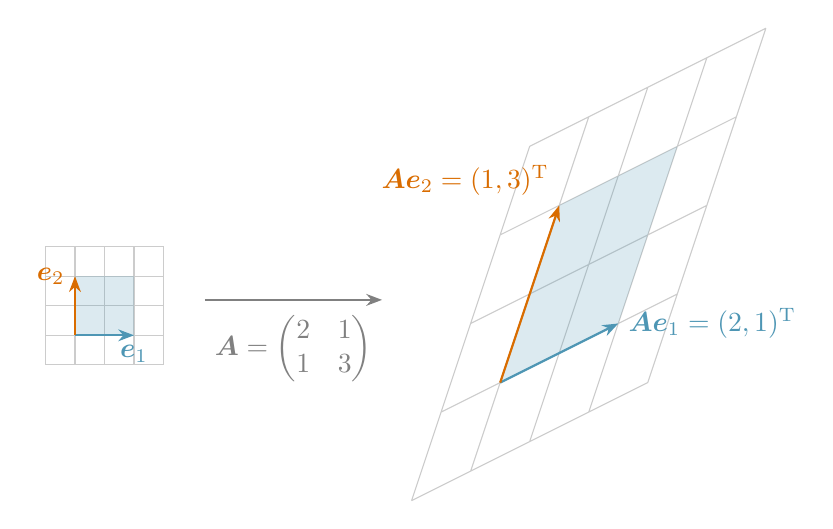
\begin{tikzpicture}[scale=0.75]
			\begin{scope}
				\draw[gray!40] (-0.5,-0.5) grid[step=0.5] (1.5,1.5);
				\fill[figblue,opacity=0.2] (0,0) rectangle (1,1);
				\draw[vec,figblue] (0,0) -- (1,0) node[below]{$\vv e_1$};
				\draw[vec,figorange] (0,0) -- (0,1) node[left]{$\vv e_2$};
			\end{scope}
			\draw[vec,thick,gray] (2.2,0.6) -- node[below=2pt]{$\vv A=\begin{pmatrix}2&1\\1&3\end{pmatrix}$} (5.2,0.6);
			\begin{scope}[xshift=7.2cm,yshift=-0.8cm]
				\begin{scope}[cm={2,1,1,3,(0,0)}]
					\draw[gray!40] (-0.5,-0.5) grid[step=0.5] (1.5,1.5);
					\fill[figblue,opacity=0.2] (0,0) rectangle (1,1);
				\end{scope}
				\draw[vec,figblue] (0,0) -- (2,1) node[right]{$\vv A\vv e_1=(2,1)^\trans$};
				\draw[vec,figorange] (0,0) -- (1,3) node[above left]{$\vv A\vv e_2=(1,3)^\trans$};
			\end{scope}
		\end{tikzpicture}
		\caption{线性变换把方格网均匀地变成平行四边形网格. 只要知道两个基向量变到哪里，整个平面的变化就确定了（定理~\ref{thm:determinedbybasis}）.}
		\label{fig:gridmap}
	\end{figure}
	\begin{theorem}\label{thm:determinedbybasis}
		设 $\vv\varepsilon_1,\ldots,\vv\varepsilon_n$ 是 $V$ 的基，$\vv\beta_1,\ldots,\vv\beta_n$ 是 $W$ 中任意 $n$ 个向量，则存在唯一的线性映射 $\mathscr T:V\to W$ 使 $\mathscr T(\vv\varepsilon_i)=\vv\beta_i$（$i=1,\ldots,n$）.
	\end{theorem}
	\begin{proof}
		唯一性：若 $\mathscr T$ 存在，则对 $\vv\alpha=\sum a_i\vv\varepsilon_i$ 必有 $\mathscr T(\vv\alpha)=\sum a_i\vv\beta_i$. 存在性：就用这个式子定义 $\mathscr T$（坐标唯一，故定义合理），直接验证它是线性的.
	\end{proof}
	
	\begin{motivebox}
		这个定理说：\textbf{线性映射完全由它在一组基上的取值决定}. 一个定义在无穷多个向量上的映射，只需要 $n$ 个向量的信息就能确定——而这 $n$ 个向量的坐标排在一起，就是一个矩阵. 这正是下文``映射 $=$ 矩阵''的根源.
	\end{motivebox}
	
	\section{核、像与秩—零化度定理}
	
	\begin{definition}
		线性映射 $\mathscr T:V\to W$ 的\textbf{核}\index{he2@核}与\textbf{像}\index{xiang4@像}分别为
		\[
		\ker\mathscr T=\{\vv\alpha\in V\mid\mathscr T(\vv\alpha)=\zero\},\qquad \imm\mathscr T=\{\mathscr T(\vv\alpha)\mid\vv\alpha\in V\}.
		\]
		它们分别是 $V$ 和 $W$ 的子空间. $\dim\imm\mathscr T$ 称为 $\mathscr T$ 的\textbf{秩}，$\dim\ker\mathscr T$ 称为 $\mathscr T$ 的\textbf{零化度}\index{ling2hua4du4@零化度}.
	\end{definition}
	
	对 $\mathscr T_{\vv A}$：$\ker\mathscr T_{\vv A}$ 就是齐次方程组 $\vv{Ax}=\zero$ 的解空间；$\imm\mathscr T_{\vv A}$ 是 $\vv A$ 的列向量张成的空间（\textbf{列空间}\index{lie4 kong1jian1@列空间}），其维数为 $\rk\vv A$.
	
	\begin{proposition}
		线性映射 $\mathscr T$ 是单射，当且仅当 $\ker\mathscr T=\{\zero\}$.
	\end{proposition}
	\begin{proof}
		$\mathscr T(\vv\alpha)=\mathscr T(\vv\beta)\iff\mathscr T(\vv\alpha-\vv\beta)=\zero\iff\vv\alpha-\vv\beta\in\ker\mathscr T$.
	\end{proof}
	
	\begin{theorem}[秩—零化度定理]\label{thm:ranknullity}\index{zhi4 ling2hua4du4 ding4li3@秩—零化度定理}
		设 $V$ 是有限维向量空间，$\mathscr T:V\to W$ 是线性映射，则
		\[
		\dim V=\dim\ker\mathscr T+\dim\imm\mathscr T.
		\]
	\end{theorem}
	\begin{proof}
		取 $\ker\mathscr T$ 的一组基 $\vv\alpha_1,\ldots,\vv\alpha_k$，用基扩张定理扩充为 $V$ 的基 $\vv\alpha_1,\ldots,\vv\alpha_k,\vv\beta_1,\ldots,\vv\beta_{m}$，$k+m=\dim V$. 只需证明 $\mathscr T(\vv\beta_1),\ldots,\mathscr T(\vv\beta_m)$ 是 $\imm\mathscr T$ 的基.
		
		生成：任意 $\vv\alpha=\sum a_i\vv\alpha_i+\sum b_j\vv\beta_j$，有 $\mathscr T(\vv\alpha)=\sum b_j\mathscr T(\vv\beta_j)$，因为 $\mathscr T(\vv\alpha_i)=\zero$.
		
		线性无关：若 $\sum c_j\mathscr T(\vv\beta_j)=\zero$，则 $\mathscr T(\sum c_j\vv\beta_j)=\zero$，即 $\sum c_j\vv\beta_j\in\ker\mathscr T$，于是 $\sum c_j\vv\beta_j=\sum d_i\vv\alpha_i$. 由 $\vv\alpha_i,\vv\beta_j$ 合起来线性无关，得所有 $c_j=0$.
	\end{proof}
	
	\begin{motivebox}
		定理说的是一种``守恒'' ：$V$ 的每一个维度，要么被 $\mathscr T$``压扁''进了核里，要么在像中``存活''下来，不多不少. 在方程组的语言里，它就是第一章的``自由变量个数 $=$ 未知量个数 $-$ 主元个数''.
	\end{motivebox}
	\begin{figure}[htbp]
		\centering
		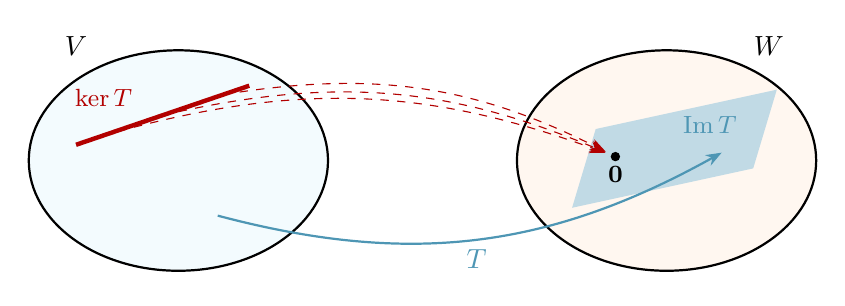
\begin{tikzpicture}
			\draw[thick,fill=customcolor!8] (0,0) ellipse (1.9 and 1.4);
			\draw[thick,fill=orange!6] (6.2,0) ellipse (1.9 and 1.4);
			\node at (-1.3,1.45) {$V$};
			\node at (7.5,1.45) {$W$};
			% 核：移到 V 的上半部
			\draw[line width=1.6pt,figred] (-1.3,0.2) -- (0.9,0.95);
			\node[figred,font=\small] at (-0.95,0.8) {$\ker\mathscr T$};
			% 像：零向量落在其内部
			\fill[figblue!35] (5.0,-0.6) -- (7.3,-0.1) -- (7.6,0.9) -- (5.3,0.4) -- cycle;
			\node[figblue,font=\small] at (6.75,0.45) {$\imm\mathscr T$};
			\node[dot] (z) at (5.55,0.05) {};
			\node[below,font=\small] at (z) {$\zero$};
			% 红色虚线从上方拱过去
			\foreach \t in {0.15,0.5,0.85}{
				\draw[->,figred,dashed,shorten >=2pt] ($(-1.3,0.2)!\t!(0.9,0.95)$) to[bend left=18] (z);
			}
			% 蓝色箭头从下方绕进像
			\draw[->,figblue,thick] (0.5,-0.7) to[bend right=22] node[below]{$\mathscr T$} (6.9,0.1);
		\end{tikzpicture}
		\caption{核被压缩成一个点（零向量），其余的维数在像中``存活''：$\dim V=\dim\ker\mathscr T+\dim\imm\mathscr T$.}
		\label{fig:kerim}
	\end{figure}
	\begin{corollary}\label{cor:nullity}
		\begin{enumerate}
			\item 设 $\vv A$ 是 $m\times n$ 矩阵，则 $\vv{Ax}=\zero$ 的解空间维数为 $n-\rk\vv A$.
			\item 若 $\dim V=\dim W$，则对线性映射 $\mathscr T:V\to W$，单射 $\iff$ 满射 $\iff$ 双射.
		\end{enumerate}
	\end{corollary}
	
	\begin{example}
		对 $\mathscr D:\mathbb{F}[x]_n\to\mathbb{F}[x]_n$，$\ker\mathscr D$ 是常数多项式全体，维数为 $1$；$\imm\mathscr D=\mathbb{F}[x]_{n-1}$，维数为 $n-1$. 二者之和为 $n$，与定理相符.
	\end{example}
	
	\section{线性映射的矩阵}
	
	\begin{definition}
		设 $\vv\varepsilon_1,\ldots,\vv\varepsilon_n$ 是 $V$ 的基，$\vv\eta_1,\ldots,\vv\eta_m$ 是 $W$ 的基，$\mathscr T:V\to W$ 线性. 设
		\[
		\mathscr T(\vv\varepsilon_j)=a_{1j}\vv\eta_1+a_{2j}\vv\eta_2+\cdots+a_{mj}\vv\eta_m\qquad(j=1,\ldots,n),
		\]
		即 $\vv A=(a_{ij})$ 的第 $j$ 列是 $\mathscr T(\vv\varepsilon_j)$ 的坐标. 形式地记为
		\[
		(\mathscr T(\vv\varepsilon_1),\ldots,\mathscr T(\vv\varepsilon_n))=(\vv\eta_1,\ldots,\vv\eta_m)\vv A,
		\]
		称 $\vv A$ 为 $\mathscr T$ 在这两组基下的\textbf{矩阵}.
	\end{definition}
	
	\begin{proposition}
		设 $\vv\alpha\in V$ 的坐标为 $\vv x$，则 $\mathscr T(\vv\alpha)$ 的坐标为 $\vv{Ax}$.
	\end{proposition}
	\begin{proof}
		$\mathscr T(\vv\alpha)=\sum_j x_j\mathscr T(\vv\varepsilon_j)=\sum_j x_j\sum_i a_{ij}\vv\eta_i=\sum_i\big(\sum_j a_{ij}x_j\big)\vv\eta_i$.
	\end{proof}
	
	\begin{example}
		在基 $1,x,x^2,x^3$ 下，$\mathscr D:\mathbb{F}[x]_4\to\mathbb{F}[x]_4$ 的矩阵为
		\[
		\begin{pmatrix}0&1&0&0\\0&0&2&0\\0&0&0&3\\0&0&0&0\end{pmatrix}.
		\]
		它是幂零矩阵——对应于``对三次多项式求导四次得零''.
	\end{example}
	
	\begin{theorem}\label{thm:composition}
		设 $\mathscr T:V\to W$，$\mathscr S:W\to U$ 线性，在取定的基下矩阵分别为 $\vv A$ 与 $\vv B$，则复合 $\mathscr S\circ\mathscr T$ 的矩阵为 $\vv{BA}$.
	\end{theorem}
	\begin{proof}
		设 $U$ 的基为 $\vv\zeta_1,\ldots,\vv\zeta_p$. 则
		\[
		\mathscr S\mathscr T(\vv\varepsilon_j)=\mathscr S\Big(\sum_k a_{kj}\vv\eta_k\Big)=\sum_k a_{kj}\sum_i b_{ik}\vv\zeta_i=\sum_i\Big(\sum_k b_{ik}a_{kj}\Big)\vv\zeta_i,
		\]
		括号中正是 $\vv{BA}$ 的 $(i,j)$ 元.
	\end{proof}
	
	\begin{motivebox}
		这就是矩阵乘法定义的``真正理由''：\textbf{矩阵乘法是线性映射复合的坐标表示}. 结合律 $(\vv{AB})\vv C=\vv A(\vv{BC})$ 之所以成立，是因为映射的复合本来就满足结合律；乘法之所以不交换，是因为``先旋转再投影''与``先投影再旋转''本来就是两件事.
	\end{motivebox}
	\begin{figure}[htbp]
		\centering
		\begin{tikzpicture}[scale=0.85]
			\foreach \dx in {0,6.4}{
				\draw[axis] (\dx-1.8,0) -- (\dx+2.6,0);
				\draw[axis] (\dx,-0.4) -- (\dx,2.6);
			}
			\draw[vec,figblue] (0,0) -- (2,1) node[right]{$\vv v$};
			\draw[vec,figorange,dashed] (0,0) -- (-1,2) node[left]{旋转后};
			\draw[dashed,gray] (-1,2) -- (-1,0);
			\draw[vec,figred] (0,0) -- (-1,0) node[below]{投影后};
			\node[sub] at (0.4,-1.0) {(a) 先旋转 $90^\circ$，\\再投影到 $x$ 轴};
			\begin{scope}[xshift=6.4cm]
				\draw[vec,figblue] (0,0) -- (2,1) node[right]{$\vv v$};
				\draw[dashed,gray] (2,1) -- (2,0);
				\draw[vec,figorange,dashed] (0,0) -- (2,0) node[below]{投影后};
				\draw[vec,figred] (0,0) -- (0,2) node[left]{旋转后};
				\node[sub] at (0.4,-1.0) {(b) 先投影到 $x$ 轴，\\再旋转 $90^\circ$};
			\end{scope}
		\end{tikzpicture}
		\caption{两种顺序得到不同的结果（红色），所以两个变换的矩阵相乘时不能交换.}
		\label{fig:noncommute}
	\end{figure}
	\section{基变换与坐标变换}
	
	同一个向量在不同的基下有不同的坐标；同一个线性变换在不同的基下有不同的矩阵. 它们之间如何换算？
	
	\begin{definition}
		设 $\vv\varepsilon_1,\ldots,\vv\varepsilon_n$ 与 $\vv\varepsilon_1',\ldots,\vv\varepsilon_n'$ 是 $V$ 的两组基，且
		\[
		(\vv\varepsilon_1',\ldots,\vv\varepsilon_n')=(\vv\varepsilon_1,\ldots,\vv\varepsilon_n)\vv P,
		\]
		即 $\vv P$ 的第 $j$ 列是新基向量 $\vv\varepsilon'_j$ 在旧基下的坐标. 称 $\vv P$ 为从旧基到新基的\textbf{过渡矩阵}\index{guo4du4 ju3zhen4@过渡矩阵}.
	\end{definition}
	
	过渡矩阵必可逆：它的列是 $n$ 个线性无关向量（新基）的坐标，由同构保持线性无关性，这 $n$ 列线性无关，秩为 $n$.
	
	\begin{theorem}
		设 $\vv\alpha$ 在旧基、新基下的坐标分别为 $\vv x,\vv x'$，则 $\vv x=\vv P\vv x'$，即 $\vv x'=\vv P^{-1}\vv x$.
	\end{theorem}
	\begin{proof}
		$\vv\alpha=(\vv\varepsilon_1',\ldots,\vv\varepsilon_n')\vv x'=(\vv\varepsilon_1,\ldots,\vv\varepsilon_n)\vv P\vv x'$，由坐标唯一性 $\vv x=\vv P\vv x'$.
	\end{proof}
	
	\begin{pitfallbox}
		基是``用旧的表示新的''（右乘 $\vv P$），坐标却是``用新的表示旧的''（$\vv x=\vv P\vv x'$），方向相反. 记忆方法：把汇率想成``1 美元 $=$ 7 元''，那么同一笔钱，以美元计的数目反而更小.
	\end{pitfallbox}
	\begin{figure}[htbp]
		\centering
		\begin{tikzpicture}[scale=0.9]
			\clip (-2.4,-1.3) rectangle (5.6,3.1);
			\draw[gray!30] (-3,-2) grid (3.5,4);
			\begin{scope}[cm={1,1,-1,1,(0,0)}]
				\draw[figorange!45,dashed] (-3,-3) grid (3,3);
			\end{scope}
			\draw[vec,gray] (0,0) -- (1,0) node[below]{$\vv\varepsilon_1$};
			\draw[vec,gray] (0,0) -- (0,1) node[left]{$\vv\varepsilon_2$};
			\draw[vec,figorange] (0,0) -- (1,1) node[above left]{$\vv\varepsilon_1'$};
			\draw[vec,figorange] (0,0) -- (-1,1) node[left]{$\vv\varepsilon_2'$};
			\draw[dashed,figorange] (0,0) -- (1.5,1.5) -- (2,1);
			\draw[vec,figred] (0,0) -- (2,1) node[right,align=left,font=\small]{$\vv\alpha$\\旧坐标 $(2,1)^\trans$\\新坐标 $(1.5,-0.5)^\trans$};
		\end{tikzpicture}
		\caption{同一个向量，两套坐标网格. 灰色是旧基，橙色是新基 $\vv\varepsilon_1'=\vv\varepsilon_1+\vv\varepsilon_2$，$\vv\varepsilon_2'=-\vv\varepsilon_1+\vv\varepsilon_2$.}
		\label{fig:changebasis}
	\end{figure}
	\begin{theorem}
		设线性变换 $\mathscr T:V\to V$ 在旧基下的矩阵为 $\vv A$，在新基下的矩阵为 $\vv B$，过渡矩阵为 $\vv P$，则
		\[
		\vv B=\vv P^{-1}\vv A\vv P.
		\]
	\end{theorem}
	\begin{proof}
		记旧基为 $(\vv\varepsilon)$，新基为 $(\vv\varepsilon')=(\vv\varepsilon)\vv P$. 由线性性，
		$\mathscr T(\vv\varepsilon')=\mathscr T(\vv\varepsilon)\vv P=(\vv\varepsilon)\vv A\vv P=(\vv\varepsilon')\vv P^{-1}\vv A\vv P$.
	\end{proof}
	
	\begin{definition}
		若存在可逆矩阵 $\vv P$ 使 $\vv B=\vv P^{-1}\vv{AP}$，称方阵 $\vv A$ 与 $\vv B$ \textbf{相似}\index{xiang1si4@相似（矩阵）}.
	\end{definition}
	
	相似是等价关系. 两个矩阵相似，意味着它们是\textbf{同一个线性变换在不同基下的矩阵}. 于是一个自然的问题出现了：能不能选一组``最好''的基，使变换的矩阵尽可能简单（比如对角矩阵）？这是第八章的主题.
	
	\begin{modelbox}{图像压缩中的换基}

		\mstep{问题} 数码图片的每个像素用红、绿、蓝三个强度 $(R,G,B)$ 存储. JPEG 压缩为什么能把文件缩小很多，而肉眼几乎看不出差别？
		
		\mstep{模型} 压缩的第一步是在 $\mathbb{R}^3$ 中换一组``基''，把 $(R,G,B)$ 变成亮度 $Y$ 与两个色度 $C_b,C_r$：
		\[
		\begin{pmatrix}Y\\C_b\\C_r\end{pmatrix}=
		\begin{pmatrix}0.299&0.587&0.114\\-0.1687&-0.3313&0.5\\0.5&-0.4187&-0.0813\end{pmatrix}
		\begin{pmatrix}R\\G\\B\end{pmatrix}.
		\]
		（JPEG/JFIF 标准还在 $C_b,C_r$ 上各加 $128$ 的偏移，见``局限''.）
		
		\mstep{求解与解读}
		\begin{itemize}
			\item 第一行系数之和为 $1$，后两行系数之和为 $0$. 所以灰色像素 $R=G=B=g$ 变为 $(g,0,0)^\trans$：灰色没有``色度''，只有亮度.
			\item 系数矩阵可逆，换基本身不损失任何信息. 但人眼对亮度远比对颜色敏感，于是可以对每 $2\times2$ 个像素只保留一组 $(C_b,C_r)$. 原来 $4$ 个像素要存 $12$ 个数，现在只需 $4+1+1=6$ 个，数据量减半.
			\item 换基不改变信息，但改变了\textbf{信息在坐标之间的分布}，让``重要的''集中到少数坐标上，``不重要的''可以舍弃. 这一思想将在第十章的奇异值分解与主成分分析中达到顶峰.
		\end{itemize}
		
		\mstep{局限} 加上 $128$ 的偏移后，变换是``线性映射 $+$ 平移''，即\textbf{仿射变换}\index{fang3she4 bian4huan4@仿射变换}，而不是线性变换（回忆：平移不保持零向量）. 另外，系数取决于所采用的标准，高清视频标准使用另一组系数.
	\end{modelbox}
	\newpage
	\ExLinearMap
	
	% =====================================================================
	\chapter{行列式}\label{ch:determinant}
	
	\paragraph*{本章地位}
	
	本章为方阵定义一个数值特征，即行列式. 从几何上看，行列式是方阵所代表的线性变换对面积或体积的有向伸缩倍数. 行列式给出了方阵可逆的数值判据，以及逆矩阵和方程组的解的显式公式（伴随矩阵与 Cramer 法则）. 本章最后用子式刻画矩阵的秩，与第三章用向量组定义的秩相互印证.
	
	\chapterhours{4}{5}{5}
	
	\begin{introduction}[学习目标]
		\item 计算排列的逆序数，按定义写出低阶行列式的展开式
		\item 运用行列式的性质把行列式化为三角形计算，运用按行（列）展开计算行列式
		\item 运用乘积公式以及``方阵可逆当且仅当行列式不为零''解决问题
		\item 求伴随矩阵，用伴随矩阵求逆矩阵，用 Cramer 法则解方程组
		\item 用子式判断矩阵的秩
	\end{introduction}
	
	\paragraph*{前置知识}
	
	第三章（初等矩阵、逆矩阵与秩）.
	
	\paragraph*{学习提示}
	\begin{itemize}
		\item 行列式的定义用于推导性质，性质用于计算. 计算时应优先用初等变换化为三角形；只有在某一行（列）的零元素较多时，才宜直接展开.
		\item 行列式的各条性质与三类初等行变换一一对应. 掌握这一对应，就能把本章与第一、三章的消元法联系起来.
		\item 行列式的几何意义可以解释乘积公式，以及行列式为零时方阵不可逆的原因. 应结合二阶、三阶的情形理解.
	\end{itemize}
	
	\newpage
	
	\begin{tcolorbox}[epigraph]
		\begin{quote}This paper shows how linear algebra can be done better without determinants.\end{quote}
		\begin{flushright}——Sheldon Axler, \textit{Down with Determinants!}\end{flushright}
		\begin{quote}本文说明，不用行列式，线性代数可以做得更好.\end{quote}
		\begin{flushright}——谢尔登·阿克斯勒\footnotemark\end{flushright}
	\end{tcolorbox}
	\footnotetext{谢尔登·阿克斯勒（1949— ），美国数学家，教材《线性代数应该这样学》的作者. 引文是其论文《打倒行列式！》（\textit{American Mathematical Monthly} 102 (1995), 139--154）摘要的第一句. 把一句``反对''行列式的话放在行列式一章的开头，是请读者带着怀疑读下去：行列式的许多用途确实可以绕开，但它度量``体积伸缩''这一几何意义，是别的工具替代不了的.}
	\section{矩阵的数字特征}
	
	考察二阶矩阵 $\vv A=\begin{pmatrix}2&1\\1&3\end{pmatrix}$ 所代表的平面线性变换. 它把标准基 $\vv e_1,\vv e_2$ 分别变为 $\vv A\vv e_1=(2,1)^\trans$ 与 $\vv A\vv e_2=(1,3)^\trans$，也就是 $\vv A$ 的两列. 原来由 $\vv e_1,\vv e_2$ 张成的单位正方形，被变成了由两列张成的平行四边形.
	
	由于线性变换把平面上的网格均匀地变成平行四边形网格，任何图形的面积都被放大了同一个倍数——就是这个平行四边形的面积. 对向量 $(x_1,y_1)^\trans$，$(x_2,y_2)^\trans$，它们张成的平行四边形的\textbf{有向面积}\index{you3xiang4 mian4ji1@有向面积}\footnote{若从第一个向量到第二个向量是逆时针方向，面积取正，否则取负. 符号记录了变换是否把平面``翻面''.}为
	\[
	S=x_1y_2-x_2y_1.
	\]
	对上面的 $\vv A$，$S=2\times3-1\times1=5$：这个变换把平面上一切图形的面积放大为 $5$ 倍.
	\begin{figure}[htbp]
		\centering
		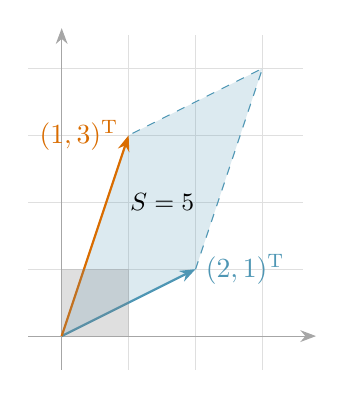
\begin{tikzpicture}[scale=0.85]
			\draw[gray!25] (-0.5,-0.5) grid (3.6,4.5);
			\draw[axis] (-0.5,0) -- (3.8,0);
			\draw[axis] (0,-0.5) -- (0,4.6);
			\fill[figblue,opacity=0.2] (0,0) -- (2,1) -- (3,4) -- (1,3) -- cycle;
			\draw[figblue,dashed] (2,1) -- (3,4) -- (1,3);
			\draw[vec,figblue] (0,0) -- (2,1) node[right]{$(2,1)^\trans$};
			\draw[vec,figorange] (0,0) -- (1,3) node[left]{$(1,3)^\trans$};
			\node[font=\small] at (1.5,2) {$S=5$};
			\fill[gray,opacity=0.25] (0,0) rectangle (1,1);
		\end{tikzpicture}
		\caption{两列张成的平行四边形面积为 $2\times3-1\times1=5$，是单位正方形（灰色）的 $5$ 倍.}
		\label{fig:detarea}
	\end{figure}
	\begin{figure}[htbp]
		\centering
		\begin{tikzpicture}[scale=0.85]
			\begin{scope}
				\coordinate (O) at (0,0); \coordinate (a) at (2.2,0.5); \coordinate (b) at (0.6,1.9);
				\fill[figblue,opacity=0.15] (O) -- (a) -- ($(a)+(b)$) -- (b) -- cycle;
				\draw[vec,figblue] (O) -- (a) node[right]{$\vv\alpha$};
				\draw[vec,figorange] (O) -- (b) node[above]{$\vv\beta$};
				\draw[->,figred] (0.8,0.18) arc[start angle=13,end angle=68,radius=0.82];
				\node[sub] at (1.3,-0.8) {(a) 逆时针\\$\det>0$};
			\end{scope}
			\begin{scope}[xshift=4.6cm]
				\coordinate (O) at (0,0); \coordinate (a) at (0.6,1.9); \coordinate (b) at (2.2,0.5);
				\fill[figorange,opacity=0.15] (O) -- (a) -- ($(a)+(b)$) -- (b) -- cycle;
				\draw[vec,figblue] (O) -- (a) node[above]{$\vv\alpha$};
				\draw[vec,figorange] (O) -- (b) node[right]{$\vv\beta$};
				\draw[->,figred] (0.26,0.79) arc[start angle=72,end angle=17,radius=0.82];
				\node[sub] at (1.3,-0.8) {(b) 顺时针（翻面）\\$\det<0$};
			\end{scope}
			\begin{scope}[xshift=9.4cm]
				\draw[gray!50] (-0.3,-0.15) -- (2.8,1.4);
				\draw[vec,figblue] (0,0) -- (2.4,1.2) node[above]{$\vv\alpha$};
				\draw[vec,figorange,thick] (0,0) -- (1.2,0.6) node[below right]{$\vv\beta$};
				\node[sub] at (1.3,-0.8) {(c) 共线，面积为零\\$\det=0$};
			\end{scope}
		\end{tikzpicture}
		\caption{行列式的符号记录方向，绝对值记录面积. $\det=0$ 意味着平面被压成了一条直线.}
		\label{fig:detsign}
	\end{figure}
	三维时，三个向量 $(x_1,y_1,z_1)^\trans$，$(x_2,y_2,z_2)^\trans$，$(x_3,y_3,z_3)^\trans$ 张成的平行六面体的有向体积为
	\[
	V = x_1y_2z_3+x_2y_3z_1+x_3y_1z_2-x_3y_2z_1-x_2y_1z_3-x_1y_3z_2.
	\]
	\begin{figure}[htbp]
		\centering
		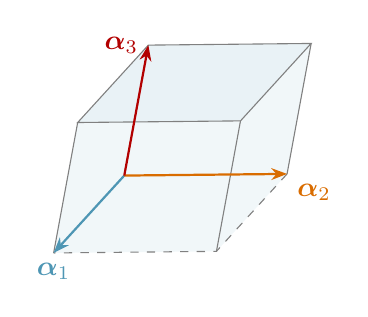
\begin{tikzpicture}[iso,scale=1.3]
			\coordinate (O) at (0,0,0);
			\coordinate (a) at (1.8,0.3,0);
			\coordinate (b) at (0.2,1.7,0.1);
			\coordinate (c) at (0.3,0.4,1.4);
			\coordinate (ab) at ($(a)+(b)$);
			\coordinate (ac) at ($(a)+(c)$);
			\coordinate (bc) at ($(b)+(c)$);
			\coordinate (abc) at ($(a)+(b)+(c)$);
			\fill[figblue,opacity=0.12] (c) -- (ac) -- (abc) -- (bc) -- cycle;
			\fill[figblue,opacity=0.08] (a) -- (ab) -- (abc) -- (ac) -- cycle;
			\fill[figblue,opacity=0.08] (b) -- (ab) -- (abc) -- (bc) -- cycle;
			\draw[gray,dashed] (b) -- (ab) -- (a);
			\draw[gray] (c) -- (ac) -- (abc) -- (bc) -- cycle;
			\draw[gray] (a) -- (ac); \draw[gray] (ab) -- (abc); \draw[gray] (b) -- (bc);
			\draw[vec,figblue] (O) -- (a) node[below]{$\vv\alpha_1$};
			\draw[vec,figorange] (O) -- (b) node[below right]{$\vv\alpha_2$};
			\draw[vec,figred] (O) -- (c) node[left]{$\vv\alpha_3$};
		\end{tikzpicture}
		\caption{三个向量张成的平行六面体. 三阶行列式是它的有向体积.}
		\label{fig:parallelepiped}
	\end{figure}
	把这些向量作为列排成矩阵，就得到二、三阶行列式.
	
	\begin{definition}
		\[
		\begin{vmatrix} a & b \\ c & d \end{vmatrix} = ad-bc,\]\[
		\begin{vmatrix} x_1 & x_2 & x_3 \\ y_1 & y_2 & y_3 \\ z_1 & z_2 & z_3 \end{vmatrix} = x_1y_2z_3+x_2y_3z_1+x_3y_1z_2-x_3y_2z_1-x_2y_1z_3-x_1y_3z_2.
		\]
	\end{definition}
	
	四维以上没有直观的``体积公式''，我们需要从这两个公式的\textbf{结构}中找到推广的方法.
	
	\section{排列与逆序}
	
	观察三阶公式. 每一项都是来自\textbf{不同行、不同列}的三个元素之积. 若把每项写成 $x_{\cdot}y_{\cdot}z_{\cdot}$（行固定为 $x,y,z$ 的顺序），下标（列号）依次为：
	\begin{itemize}
		\item 正项：$123$，$231$，$312$；
		\item 负项：$321$，$213$，$132$.
	\end{itemize}
	所有 $3!=6$ 种列号排列恰好各出现一次. 是什么决定了符号？
	
	\begin{definition}
		由 $1,2,\ldots,n$ 组成的有序数组 $i_1i_2\cdots i_n$ 称为一个 $n$ 级\textbf{排列}\index{pai2lie4@排列}，共有 $n!$ 个. 若在排列中一对数 $i_s,i_t$（$s<t$）满足 $i_s>i_t$，称它们构成一个\textbf{逆序}\index{ni4xu4@逆序}. 逆序的总数称为该排列的\textbf{逆序数}\index{ni4xu4shu4@逆序数}，记为 $\tau(i_1i_2\cdots i_n)$. 逆序数为偶数的排列称为\textbf{偶排列}\index{ou3 pai2lie4@偶排列}，为奇数的称为\textbf{奇排列}\index{ji1 pai2lie4@奇排列}.
	\end{definition}
	
	计算可知 $\tau(123)=0$，$\tau(231)=\tau(312)=2$，都是偶排列；$\tau(321)=3$，$\tau(213)=\tau(132)=1$，都是奇排列. 正项对应偶排列，负项对应奇排列！
	
	\begin{lemma}\label{lem:transposition}
		交换排列中的任意两个数，排列的奇偶性改变.
	\end{lemma}
	\begin{proof}
		先看交换相邻两数：只有这两个数之间的先后关系改变，其他任何一对数的相对顺序都不变，所以逆序数恰好增加或减少 $1$. 再看交换位置 $s<t$ 上的两个数：可以先把位置 $t$ 上的数逐次与左边相邻的数交换，移到位置 $s$（$t-s$ 次），再把原来位置 $s$ 上的数（现在在 $s+1$）逐次右移到位置 $t$（$t-s-1$ 次），共 $2(t-s)-1$ 次相邻交换，是奇数次.
	\end{proof}
	
	\section{\texorpdfstring{$n$}{n} 阶行列式}
	
	\begin{definition}
		$n$ 阶方阵 $\vv A=(a_{ij})$ 的\textbf{行列式}\index{hang2lie4shi4@行列式}定义为
		\[
		\det\vv A=|\vv A|=\begin{vmatrix} a_{11}&\cdots&a_{1n}\\ \vdots&&\vdots\\ a_{n1}&\cdots&a_{nn}\end{vmatrix}
		=\sum_{i_1i_2\cdots i_n}(-1)^{\tau(i_1i_2\cdots i_n)}a_{1i_1}a_{2i_2}\cdots a_{ni_n},
		\]
		求和取遍全部 $n!$ 个 $n$ 级排列.
	\end{definition}
	
	$n=2,3$ 时这与上一节的公式一致. 这个定义的每一项都是``每行取一个、每列取一个''的乘积，符号由列号排列的奇偶决定.
	
	\begin{remark}
		按定义计算 $n$ 阶行列式需要 $n!$ 项，每项 $n-1$ 次乘法. $n=20$ 时 $20!\approx2.4\times10^{18}$，即使每秒运算十亿次也要算一千多年. 而用下一节的性质化为三角形，运算量只是 $n^3$ 量级. 定义用来\textbf{推导性质}，性质用来\textbf{计算}.
	\end{remark}
	
	\section{行列式的性质}
	
	\begin{dprop}{}{det-triangular}
		三角矩阵的行列式等于主对角元之积.
	\end{dprop}
	\begin{proof}
		以上三角为例. 一项 $a_{1i_1}\cdots a_{ni_n}$ 非零，要求每个 $a_{ki_k}\ne0$，即 $i_k\ge k$ 对一切 $k$ 成立. 由 $i_n\ge n$ 得 $i_n=n$，再由 $i_{n-1}\ge n-1$ 且 $\ne n$ 得 $i_{n-1}=n-1$，依次类推，只有排列 $12\cdots n$ 一项可能非零.
	\end{proof}
	
	\begin{dprop}{}{det-transpose}
		$\det\vv A^\trans=\det\vv A$. 因此下面关于``行''的性质对``列''同样成立.
	\end{dprop}
	\begin{proof}
		$\det\vv A$ 的一项 $a_{1i_1}\cdots a_{ni_n}$ 把因子按列号重新排序，写成 $a_{j_11}a_{j_22}\cdots a_{j_nn}$，这正是 $\det\vv A^\trans$ 中对应列号排列 $j_1\cdots j_n$ 的项. 排列 $j_1\cdots j_n$ 与 $i_1\cdots i_n$ 互为``逆排列''：$i_s=t\iff j_t=s$. 位置对 $(s,s')$（$s<s'$）在 $i$ 中构成逆序，当且仅当数对 $(i_{s'},i_s)$ 对应的位置在 $j$ 中构成逆序，这是逆序之间的一一对应，所以两个排列的逆序数相等，符号相同. 而 $i\mapsto j$ 是全体排列之间的双射，故两个和式相等.
	\end{proof}
	
	\begin{dprop}{多重线性}{det-linear}
		行列式对每一行都是``线性''的：某一行乘以 $c$，行列式乘以 $c$；若某一行是两组数之和，则行列式可拆为两个行列式之和（其余行不变）：
		\[
		\begin{vmatrix} \vdots \\ \vv a+\vv b\\ \vdots\end{vmatrix}=\begin{vmatrix} \vdots \\ \vv a\\ \vdots\end{vmatrix}+\begin{vmatrix} \vdots \\ \vv b\\ \vdots\end{vmatrix}.
		\]
		特别地，有一行全为零的行列式等于零.
	\end{dprop}
	\begin{proof}
		定义中每一项恰含第 $i$ 行的一个元素，作为因子出现一次.
	\end{proof}
	
	\begin{dprop}{反对称}{det-swap}
		交换两行，行列式变号.
	\end{dprop}
	\begin{proof}
		设交换第 $s,t$ 行得 $\vv B$. 
		
		$\det\vv B$ 中对应列号排列 $\cdots i_s\cdots i_t\cdots$ 的项是 $a_{1i_1}\cdots a_{ti_s}\cdots a_{si_t}\cdots a_{ni_n}$，这恰是 $\det\vv A$ 中对应列号排列 $\cdots i_t\cdots i_s\cdots$（交换了两个位置）的项. 由引理~\ref{lem:transposition}，两者符号相反. 遍历所有排列即得 $\det\vv B=-\det\vv A$.
	\end{proof}
	
	\begin{dprop}{}{det-equalrows}
		两行相同或成比例的行列式等于零.
	\end{dprop}
	\begin{proof}
		两行相同时，交换这两行得 $D=-D$，故 $D=0$.\footnote{这一步用到 $2D=0\Rightarrow D=0$，在数域中自然成立.} 成比例时，由多重线性提出比例因子化为相同的情形.
	\end{proof}
	
	\begin{dprop}{}{det-addrow}
		把某一行的 $c$ 倍加到另一行，行列式不变.
	\end{dprop}
	\begin{proof}
		由多重线性拆成两个行列式之和，其中一个就是原行列式，另一个有两行成比例，等于零.
	\end{proof}
	
	性质~\ref{prop:det-linear}、\ref{prop:det-swap}、\ref{prop:det-addrow} 恰好描述了三类初等行变换对行列式的影响：倍乘乘以 $k$，对换变号，倍加不变. 于是\textbf{计算行列式的标准方法}是：用初等行（列）变换化为上三角形，记录过程中的系数变化，再取对角元之积. 这种在行列式中``制造零''的做法，正是第三章打洞的思想在数的层面上的体现.
	
	\begin{example}
		\[
		\begin{vmatrix}1&2&3\\2&3&1\\3&1&2\end{vmatrix}
		\xlongequal[r_3-3r_1]{r_2-2r_1}
		\begin{vmatrix}1&2&3\\0&-1&-5\\0&-5&-7\end{vmatrix}
		\xlongequal{r_3-5r_2}
		\begin{vmatrix}1&2&3\\0&-1&-5\\0&0&18\end{vmatrix}=-18.
		\]
	\end{example}
	
	\section{按行（列）展开}
	
	\begin{definition}
		在 $n$ 阶行列式中划去第 $i$ 行、第 $j$ 列，余下元素按原顺序组成的 $n-1$ 阶行列式记为 $M_{ij}$，称为 $a_{ij}$ 的\textbf{余子式}\index{yu2zi3shi4@余子式}；$A_{ij}=(-1)^{i+j}M_{ij}$ 称为 $a_{ij}$ 的\textbf{代数余子式}\index{dai4shu4 yu2zi3shi4@代数余子式}.
	\end{definition}
	
	\begin{theorem}[Laplace 展开]\label{thm:expansion}\index{laplace zhan3kai1@Laplace 展开}
		对任意 $i,j$，
		\[
		\det\vv A=\sum_{k=1}^n a_{ik}A_{ik}\ \ (\text{按第 } i \text{ 行展开})=\sum_{k=1}^n a_{kj}A_{kj}\ \ (\text{按第 } j \text{ 列展开}).
		\]
	\end{theorem}
	\begin{proof}
		\textbf{第一步：按第一行展开.} 把定义中的 $n!$ 项按 $i_1=j$ 分组. 对固定的 $j$，剩下的列号 $i_2\cdots i_n$ 是 $\{1,\ldots,n\}\setminus\{j\}$ 的一个排列，记为 $\sigma'$. $i_1=j$ 排在最前，它与后面比它小的 $j-1$ 个数构成逆序，故
		\[
		\tau(j\,i_2\cdots i_n)=(j-1)+\tau(\sigma').
		\]
		而 $a_{2i_2}\cdots a_{ni_n}$ 带符号 $(-1)^{\tau(\sigma')}$ 求和，恰是 $M_{1j}$ 的定义（把剩余列号按大小重新编为 $1,\ldots,n-1$ 不改变任何两数的大小关系，从而不改变逆序数）. 于是
		\[
		\det\vv A=\sum_{j=1}^n(-1)^{j-1}a_{1j}M_{1j}=\sum_{j=1}^n(-1)^{1+j}a_{1j}M_{1j}=\sum_{j=1}^na_{1j}A_{1j}.
		\]
		
		\textbf{第二步：按第 $i$ 行展开.} 把第 $i$ 行依次与上面相邻的行交换，经 $i-1$ 次交换移到第一行，其余各行相对顺序不变. 新矩阵按第一行展开时，$a_{ij}$ 的余子式恰好是原来的 $M_{ij}$. 由性质~\ref{prop:det-swap}，
		\[
		\det\vv A=(-1)^{i-1}\sum_j(-1)^{1+j}a_{ij}M_{ij}=\sum_j(-1)^{i+j}a_{ij}M_{ij}.
		\]
		
		\textbf{第三步：按列展开.} 对 $\vv A^\trans$ 按行展开，再用性质~\ref{prop:det-transpose}.
	\end{proof}
	
	\begin{corollary}[异乘变零]\label{cor:alien}
		当 $i\ne j$ 时，$\sum_{k=1}^n a_{ik}A_{jk}=0$.
	\end{corollary}
	\begin{proof}
		左边是把 $\vv A$ 的第 $j$ 行换成第 $i$ 行后，按第 $j$ 行展开得到的行列式. 这个行列式有两行相同，等于零.
	\end{proof}
	
	\begin{example}[（Vandermonde 行列式）]\index{vandermonde hang2lie4shi4@Vandermonde 行列式}
		\[
		\begin{vmatrix}1&1&\cdots&1\\ x_1&x_2&\cdots&x_n\\ \vdots&\vdots&&\vdots\\ x_1^{n-1}&x_2^{n-1}&\cdots&x_n^{n-1}\end{vmatrix}=\prod_{1\le i<j\le n}(x_j-x_i).
		\]
		证明：从最后一行起，每一行减去上一行的 $x_1$ 倍，再按第一列展开，并提出各列公因子 $(x_j-x_1)$，得到一个 $n-1$ 阶 Vandermonde 行列式，然后归纳. 细节留作练习.
	\end{example}
	
	\section{乘积公式与可逆性}
	
	\begin{theorem}\label{thm:detproduct}
		对 $n$ 阶方阵 $\vv A,\vv B$，
		\begin{enumerate}
			\item $\vv A$ 可逆当且仅当 $\det\vv A\ne0$；
			\item $\det(\vv{AB})=\det\vv A\cdot\det\vv B$.
		\end{enumerate}
	\end{theorem}
	\begin{proof}
		由性质~\ref{prop:det-linear}—\ref{prop:det-addrow}，对任意初等矩阵 $\vv E$ 和方阵 $\vv M$，有 $\det(\vv{EM})=\det\vv E\cdot\det\vv M$，其中 $\det\vv E(i,j)=-1$，$\det\vv E(i(k))=k$，$\det\vv E(i,j(c))=1$，都不为零.
		
		(1) 设 $\vv A$ 的简化阶梯形为 $\vv R=\vv E_k\cdots\vv E_1\vv A$，则 $\det\vv R=\det\vv E_k\cdots\det\vv E_1\cdot\det\vv A$，且 $\det\vv E_i\neq 0$. 若 $\vv A$ 可逆，$\vv R=\vv I$，$\det\vv R=1$，故 $\det\vv A\ne0$. 若 $\vv A$ 不可逆，$\vv R$ 有零行，$\det\vv R=0$，故 $\det\vv A=0$.
		
		(2) 若 $\vv A$ 可逆，把它写成初等矩阵之积 $\vv E_1\cdots\vv E_k$，反复使用 $\det(\vv{EM})=\det\vv E\det\vv M$ 即得. 若 $\vv A$ 不可逆，则 $\vv{AB}$ 也不可逆（否则由 $\vv A(\vv B(\vv{AB})^{-1})=\vv I$ 及推论~\ref{cor:onesided}，$\vv A$ 可逆），两边都为零.
	\end{proof}
	
	\begin{motivebox}
		从几何上看，乘积公式几乎是不言自明的：先做变换 $\vv B$，体积放大 $\det\vv B$ 倍；再做 $\vv A$，又放大 $\det\vv A$ 倍. 而 $\det\vv A=0$ 意味着变换把空间压成了更低维的``薄片''，信息丢失，自然无法撤销.
	\end{motivebox}
	
	\begin{definition}
		称 $\vv A^*=(A_{ji})$，即 $(i,j)$ 元为 $A_{ji}$ 的矩阵，为 $\vv A$ 的\textbf{伴随矩阵}\index{ban4sui2 ju3zhen4@伴随矩阵}. 注意下标的转置.
	\end{definition}
	
	\begin{theorem}
		$\vv{AA}^*=\vv A^*\vv A=(\det\vv A)\vv I$. 因此当 $\det\vv A\ne0$ 时，$\vv A^{-1}=\dfrac{1}{\det\vv A}\vv A^*$.
	\end{theorem}
	\begin{proof}
		$\vv{AA}^*$ 的 $(i,j)$ 元为 $\sum_k a_{ik}A_{jk}$，$i=j$ 时由展开定理等于 $\det\vv A$，$i\ne j$ 时由推论~\ref{cor:alien} 等于 $0$. $\vv A^*\vv A$ 同理按列讨论.
	\end{proof}
	
	\begin{theorem}[Cramer 法则]\index{cramer fa3ze2@Cramer 法则}
		若 $n$ 阶方阵 $\vv A$ 满足 $D=\det\vv A\ne0$，则方程组 $\vv{Ax}=\vv b$ 有唯一解
		\[
		x_j=\frac{D_j}{D}\qquad(j=1,\ldots,n),
		\]
		其中 $D_j$ 是把 $\vv A$ 的第 $j$ 列换成 $\vv b$ 所得矩阵的行列式.
	\end{theorem}
	\begin{proof}
		$\vv x=\vv A^{-1}\vv b=\frac1D\vv A^*\vv b$，其第 $j$ 个分量为 $\frac1D\sum_i A_{ij}b_i$，而 $\sum_i b_iA_{ij}$ 正是 $D_j$ 按第 $j$ 列展开.
	\end{proof}
	
	\begin{remark}
		Cramer 法则的理论意义大于计算意义：它说明解``连续地依赖于''系数，并给出了显式公式. 但实际求解时，计算 $n+1$ 个行列式远不如一次消元划算.
	\end{remark}
		\section{子式与矩阵的秩}\label{sec:minorrank}
	
	第三章用行（列）向量组的秩定义了矩阵的秩，求秩要做初等变换. 行列式给出了另一种刻画：看矩阵里``藏着''多大的非零行列式.
	
	\begin{definition}
		设 $\vv A$ 是 $m\times n$ 矩阵，$1\le k\le\min\{m,n\}$. 任取 $\vv A$ 的 $k$ 行与 $k$ 列，位于这些行、列交叉处的 $k^2$ 个元素按原来的相对位置组成的 $k$ 阶行列式，称为 $\vv A$ 的一个 $k$ 阶\textbf{子式}\index{zi3shi4@子式}(minor). 当 $\vv A$ 是方阵且所取的行号与列号相同时，称为\textbf{主子式}\index{zhu3zi3shi4@主子式}(principal minor)；若所取的恰是前 $k$ 行与前 $k$ 列，称为 $k$ 阶\textbf{顺序主子式}\index{shun4xu4 zhu3zi3shi4@顺序主子式}(leading principal minor).
	\end{definition}
	
	例如，余子式 $M_{ij}$ 就是 $n$ 阶方阵的一个 $n-1$ 阶子式.
	
	\begin{theorem}\label{thm:minorrank}
		矩阵的秩等于它的非零子式的最高阶数. 即 $\rk\vv A=r\ge1$ 当且仅当 $\vv A$ 有一个 $r$ 阶子式不为零，而所有 $r+1$ 阶子式（如果有）都为零.
	\end{theorem}
	\begin{proof}
		设 $\rk\vv A=r\ge1$.
		
		\textbf{有一个 $r$ 阶子式不为零.} $\vv A$ 的行秩为 $r$，取它的 $r$ 个线性无关的行，组成 $r\times n$ 矩阵 $\vv B$，则 $\rk\vv B=r$. 由定理~\ref{thm:rowcolrank}，$\vv B$ 的列秩也是 $r$，取它的 $r$ 个线性无关的列，组成 $r$ 阶方阵 $\vv C$. $\vv C$ 满秩，由推论~\ref{cor:rankinvariant}(3) 与定理~\ref{thm:detproduct}，$\det\vv C\ne0$. 而 $\det\vv C$ 正是 $\vv A$ 的一个 $r$ 阶子式.
		
		\textbf{高于 $r$ 阶的子式都为零.} 任取 $k>r$ 行、$k$ 列组成 $k$ 阶子式 $\det\vv D$. $\vv A$ 的这 $k$ 行线性相关（第二章章末习题~\ref{ex:vs:A20}），即有不全为零的 $c_1,\ldots,c_k$ 使这 $k$ 行的组合为零行. 只看其中被选中的 $k$ 列的分量，同一组系数也使 $\vv D$ 的 $k$ 行组合为零. 故 $\vv D$ 的行线性相关，$\det\vv D=0$.
	\end{proof}
	
	\begin{corollary}\label{cor:minorrank}
		\begin{enumerate}
			\item $\rk\vv A\ge k$，当且仅当 $\vv A$ 有一个不为零的 $k$ 阶子式；
			\item $n$ 阶方阵满秩，当且仅当它的行列式不为零.
		\end{enumerate}
	\end{corollary}
	\begin{proof}
		(1) 若 $\rk\vv A\ge k$，取 $k$ 个线性无关的行，再按定理证明的第一步取 $k$ 列即可；反之由定理证明的第二步，非零的 $k$ 阶子式说明 $\vv A$ 有 $k$ 个线性无关的行. (2) 是 (1) 取 $k=n$ 的情形.
	\end{proof}
	
	\begin{example}
		求 $\vv A=\begin{pmatrix}1&2&3\\2&4&6\\1&0&1\end{pmatrix}$ 的秩.
	\end{example}
	\begin{solution}
		唯一的 $3$ 阶子式是 $\det\vv A$，前两行成比例，它为零，故 $\rk\vv A\le2$. 取第 $1,3$ 行与第 $1,2$ 列，$\begin{vmatrix}1&2\\1&0\end{vmatrix}=-2\ne0$，故 $\rk\vv A=2$.
	\end{solution}
	
	\begin{remark}
		求秩时，子式通常比初等变换麻烦得多. 这个定理的价值在于理论上的刻画. 例如它说明：一个非零子式在矩阵元素作微小改动后仍不为零，所以\textbf{秩在微小扰动下不会降低，只可能升高}. 带测量误差的数据矩阵因此几乎总是满秩的，``数据的真实秩''要用第十章的奇异值来判断.
	\end{remark}
	\begin{modelbox}{投入产出（续）：经济能否运转与产业乘数}
		\mstep{问题} 回到两部门模型 $(\vv I-\vv A)\vv x=\vv d$，$\vv A=\begin{pmatrix}0.2&0.3\\0.4&0.1\end{pmatrix}$. 两个问题：(1) 这个经济体是否\textbf{对任何}非负的最终需求都能给出非负的产出？(2) 某部门的最终需求增加 $1$ 单位，各部门产出各需增加多少？
		
		\mstep{模型与求解} 对问题 (1)，经济学中的 \textbf{Hawkins–Simon 条件}（1949）指出：对元素非负的 $\vv A$，答案为``是''当且仅当 $\vv I-\vv A$ 的各阶顺序主子式都为正. 这里
		\[0.8>0,\qquad \begin{vmatrix}0.8&-0.3\\-0.4&0.9\end{vmatrix}=0.72-0.12=0.60>0,\]
		条件满足. 一阶条件 $1-a_{11}>0$ 的经济含义很直观：一个部门生产 $1$ 单位产品，消耗的自身产品不能超过 $1$ 单位，否则越生产越``亏''.
		
		对问题 (2)，用 Cramer 法则写出解的显式公式：
		\[
		x_1=\frac{\begin{vmatrix}d_1&-0.3\\d_2&0.9\end{vmatrix}}{0.6}=\frac{0.9d_1+0.3d_2}{0.6},\qquad
		x_2=\frac{\begin{vmatrix}0.8&d_1\\-0.4&d_2\end{vmatrix}}{0.6}=\frac{0.4d_1+0.8d_2}{0.6}.
		\]
		代入 $\vv d=(110,170)^\trans$ 得 $\vv x=(250,300)^\trans$，与第一章一致. 而且可以直接读出\textbf{边际效应}：$d_2$ 每增加 $1$，$x_1$ 增加 $0.3/0.6=0.5$. 这种``参数变动一点，均衡解变动多少''的分析，经济学中称为\textbf{比较静态分析}\index{bi3jiao4 jing4tai4 fen1xi1@比较静态分析}，Cramer 法则是它的标准工具.
		
		\mstep{解读} 把四个边际效应排成矩阵，正是列昂惕夫逆矩阵
		\[(\vv I-\vv A)^{-1}\approx\begin{pmatrix}1.500&0.500\\0.667&1.333\end{pmatrix}.\]
		它的列和称为\textbf{产出乘数}\index{chan3chu1 cheng2shu4@产出乘数}：第一列和约为 $2.17$，表示对农业的最终需求增加 $1$ 单位，会带动全社会总产出增加约 $2.17$ 单位；第二列和约为 $1.83$. 乘数大的部门对上游的拉动作用强，在投入产出分析中常被视为``关联度高''的部门.
		
		\mstep{局限} 模型假设消耗系数固定：技术不变、规模报酬不变、投入之间不能相互替代，也没有价格机制. 所以它适合分析短期、小幅度的需求冲击，不适合预测长期结构变化.
	\end{modelbox}
	\begin{historybox}{行列式比矩阵更早}
		1683 年，日本数学家关孝和在研究消元问题时已经使用了行列式的思想\cite{seki1683kaifukudai,kline1972mathematical}；1693 年，莱布尼茨在给洛必达的信中也独立地提出了类似的想法\cite{muir1906theory}. 1750 年，克拉默（G.~Cramer）发表了以他命名的法则\cite{cramer1750introduction}. 1812 年前后，柯西系统地建立了行列式理论，并证明了乘积公式\cite{cauchy1815memoire}. 行列式在矩阵概念出现之前已经发展了一个半世纪.
	\end{historybox}
	
	\begin{codebox}{行列式的计算难题}
		\mstep{目标} 用``按定义''和``按性质打洞''两种方法计算行列式，比较它们的速度.
		
		\mstep{准备} \texttt{itertools.permutations}；\texttt{fractions.Fraction}；\texttt{time.perf\_counter}；用于对照的 \texttt{numpy.linalg.det}.
		
		\mstep{任务}
		\begin{enumerate}
			\item 写函数 \texttt{inversions(p)} 计算排列的逆序数，再写 \texttt{det\_by\_definition(A)}：枚举全部 $n!$ 个排列，按定义求和.
			\item 写函数 \texttt{det\_by\_elimination(A)}：用倍加化为上三角形，遇到零主元就对换并变号，最后取对角元之积. 全程用 \texttt{Fraction}.
			\item 用``行列式的性质''一节的例题检验两个函数，再用 \texttt{numpy.linalg.det} 算一次.
			\item 对 $n=5,6,7,8,9$ 各生成一个随机整数矩阵，记录两个函数的耗时，列成表.
		\end{enumerate}
		
		\mstep{检查点} 两个函数都恰好得到 $-18$；\texttt{numpy.linalg.det} 给出的结果应当非常接近 $-18$ ；按定义计算时，$n$ 每增加 $1$，耗时大约乘以 $n$，$n=9$ 时约需 $1$ 秒.
		
		\mstep{思考}
		\begin{enumerate}
			\item 根据你的表，估计按定义计算一个 $20$ 阶行列式需要多少年. 打洞法的耗时随 $n$ 怎样增长？
			\item \texttt{numpy} 对一个整数矩阵为什么给不出整数？它用的是这两种方法中的哪一种？
		\end{enumerate}
	\end{codebox}
	\ExDeterminant
	
	% =====================================================================
	\chapter{线性方程组解的结构}\label{ch:solutions}

	\paragraph*{本章地位}
	
	本章是第一部分的总结. 第一章给出了求解方程组的算法，第二至五章建立了秩、维数、线性映射与行列式的语言. 本章用这些语言完整地描述线性方程组的解集：解是否存在、是否唯一，齐次方程组的解空间及其基础解系，以及非齐次方程组的解集与齐次方程组解空间的关系. 64、72 学时方案还将讨论子空间的方程表示、方程组能够唯一确定哪些量，以及矩阵的秩不等式.
	
	\chapterhours{4}{5}{6}
	
	\begin{introduction}[学习目标]
		\item 用秩判断线性方程组是否有解、解是否唯一
		\item 求齐次方程组的基础解系，写出非齐次方程组的通解
		\item 说明非齐次方程组的解集与对应齐次方程组的解空间之间的关系
		\item 在子空间的参数表示与方程表示之间相互转化（64 学时起），解矩阵方程，运用 Sylvester 不等式
		\item 判断方程组能否唯一确定给定的量
	\end{introduction}
	
	\paragraph*{前置知识}
	
	第一章至第五章，特别是矩阵的秩、秩—零化度定理与行列式.
	
	\paragraph*{学习提示}
	\begin{itemize}
		\item 本章的结论都可以用三种语言表述：方程组、矩阵方程 $\vv{Ax}=\vv b$，以及线性映射的核与像. 能在三种表述之间相互转换，是本章的主要目标.
		\item 解集的结构可以概括为：非齐次方程组的通解等于它的一个特解加上对应齐次方程组的通解；齐次方程组的解空间是子空间，其维数由系数矩阵的秩决定.
		\item 本章的建模实验关注的是解的结构本身的含义，例如自由度从何而来、哪些量能被确定，而不只是计算结果. 阅读时应注意这一点.
	\end{itemize}
	
	\newpage
	
	% ---------------------------------------------------------------------
	\begin{tcolorbox}[epigraph]
	\begin{quote}知之为知之，不知为不知，是知也.\end{quote}
	\begin{flushright}——《论语·为政》\end{flushright}
	\end{tcolorbox}
	\section{解的存在性与唯一性}\label{sec:sol-exist}
	
	\begin{theorem}[Rouché–Capelli]\label{thm:rouche}\index{rouche capelli ding4li3@Rouché–Capelli 定理}
		设 $\vv A$ 为 $m\times n$ 矩阵. 方程组 $\vv{Ax}=\vv b$
		\begin{enumerate}
			\item 有解，当且仅当 $\rk\vv A=\rk(\vv A\mid\vv b)$；
			\item 有唯一解，当且仅当 $\rk\vv A=\rk(\vv A\mid\vv b)=n$.
		\end{enumerate}
	\end{theorem}
	\begin{proof}
		(1) $\vv{Ax}=\vv b$ 有解 $\iff$ $\vv b$ 可由 $\vv A$ 的列向量线性表出. 若 $\vv b$ 可由 $\vv A$ 的列线性表出，则 $\vv A$ 的列向量组与 $(\vv A\mid\vv b)$ 的列向量组等价，秩相等. 反之若秩相等，取 $\vv A$ 列向量组的一个极大无关组，它也是 $(\vv A\mid\vv b)$ 列向量组中含 $\rk(\vv A\mid\vv b)$ 个向量的无关组，因而是后者的极大无关组，$\vv b$ 可由它线性表出.
		
		(2) 若 $\vv x_0,\vv x_1$ 都是解，则 $\vv A(\vv x_1-\vv x_0)=\zero$. 所以有解时，解唯一 $\iff$ $\vv{Ax}=\zero$ 只有零解 $\iff$ $\dim\ker\vv A=n-\rk\vv A=0$.
	\end{proof}
	
	这与第一章定理~\ref{thm:solvability} 完全一致：``没有 $(0,\ldots,0\mid d)$ 行''，就是``加上 $\vv b$ 这一列后主元个数不增加''.
	
	\begin{corollary}\label{cor:sol-fullrank}
		设 $\vv A$ 为 $m\times n$ 矩阵.
		\begin{enumerate}
			\item 若 $\rk\vv A=m$（\textbf{行满秩}\index{hang2 man3zhi4@行满秩}），则对\textbf{任意} $\vv b$，$\vv{Ax}=\vv b$ 都有解；
			\item 若 $\rk\vv A=n$（\textbf{列满秩}\index{lie4 man3zhi4@列满秩}），则对任意 $\vv b$，$\vv{Ax}=\vv b$ \textbf{至多}有一个解；
			\item 当 $m=n$ 时，以下条件等价：对任意 $\vv b$ 都有唯一解；$\rk\vv A=n$；$\vv A$ 可逆；$\det\vv A\ne0$.
		\end{enumerate}
	\end{corollary}
	\begin{proof}
		(1) $(\vv A\mid\vv b)$ 只有 $m$ 行，$m=\rk\vv A\le\rk(\vv A\mid\vv b)\le m$. (2) 由定理第 (2) 部分的证明. (3) 由 (1)(2)、定理~\ref{thm:invertible} 与定理~\ref{thm:detproduct}.
	\end{proof}
	
	\begin{motivebox}
		行满秩说的是``约束彼此独立、没有自相矛盾的可能''，所以总有解；列满秩说的是``未知量彼此独立、没有可以互相替代的方向''，所以至多一解. 存在性看行，唯一性看列. 两者兼得只可能在方阵中发生.
	\end{motivebox}
	
	\begin{example}\label{eg:lambda}
		讨论 $\lambda$ 取何值时，方程组
		\[\left\{\begin{array}{l}
			\lambda x+y+z=1,\\ x+\lambda y+z=\lambda,\\ x+y+\lambda z=\lambda^2
		\end{array}\right.\]
		有唯一解、无解或有无穷多解.
	\end{example}
	\begin{solution}
		第一章章末习题~\ref{ex:elim:B16} 用消元法讨论过这个问题，现在用秩与行列式重新组织论证. 系数行列式为
		\[
		\begin{vmatrix}\lambda&1&1\\1&\lambda&1\\1&1&\lambda\end{vmatrix}=(\lambda+2)(\lambda-1)^2
		\]
		（把各列加到第一列，提出公因子 $\lambda+2$，再化为三角形）.
		\begin{itemize}
			\item $\lambda\ne1$ 且 $\lambda\ne-2$：由推论~\ref{cor:sol-fullrank}(3)，有唯一解. 用 Cramer 法则或消元可得
			\[x=-\frac{\lambda+1}{\lambda+2},\qquad y=\frac{1}{\lambda+2},\qquad z=\frac{(\lambda+1)^2}{\lambda+2}.\]
			\item $\lambda=1$：三个方程都是 $x+y+z=1$，$\rk\vv A=\rk(\vv A\mid\vv b)=1<3$，有无穷多解，自由度为 $2$.
			\item $\lambda=-2$：$\rk\vv A=2$. 把增广矩阵的三行相加得 $(0,0,0\mid 3)$，故 $\rk(\vv A\mid\vv b)=3\ne2$，无解.
		\end{itemize}
	\end{solution}
	
	\paragraph*{几何解释：空间中三个平面的位置关系.} 在 $\mathbb{R}^3$ 中，一个方程 $a_1x+a_2y+a_3z=b$（$a_i$ 不全为零）表示一个平面. 三个方程联立，就是问三个平面有没有公共点. 记 $r=\rk\vv A$，$\bar r=\rk(\vv A\mid\vv b)$，则全部情形如下.
	
	\begin{table}[htbp]
		\centering
		\begin{tabular}{ccl}
			\toprule
			$r$ & $\bar r$ & 三个平面的位置关系 \\
			\midrule
			$3$ & $3$ & 交于唯一一点 \\
			$2$ & $2$ & 交于一条公共直线 \\
			$1$ & $1$ & 三个平面重合 \\
			$2$ & $3$ & 没有公共点：两两相交成三条平行直线，或两个平行、第三个与它们相交 \\
			$1$ & $2$ & 没有公共点：三个平面互相平行，且不全重合 \\
			\bottomrule
		\end{tabular}
		\caption{三个平面的位置关系与秩}
		\label{tab:threeplanes}
	\end{table}
	\begin{figure}[htbp]
		\centering
		\begin{tikzpicture}
			% (a) three planes through a point
			\begin{scope}[iso2,scale=0.6]
				\fill[figblue,opacity=0.18] (-1.3,-1.3,0) -- (1.3,-1.3,0) -- (1.3,1.3,0) -- (-1.3,1.3,0) -- cycle;
				\fill[figorange,opacity=0.18] (-1.3,0,-1.2) -- (1.3,0,-1.2) -- (1.3,0,1.2) -- (-1.3,0,1.2) -- cycle;
				\fill[figgreen,opacity=0.18] (0,-1.3,-1.2) -- (0,1.3,-1.2) -- (0,1.3,1.2) -- (0,-1.3,1.2) -- cycle;
				\draw[figblue] (-1.3,-1.3,0) -- (1.3,-1.3,0) -- (1.3,1.3,0) -- (-1.3,1.3,0) -- cycle;
				\draw[figorange] (-1.3,0,-1.2) -- (1.3,0,-1.2) -- (1.3,0,1.2) -- (-1.3,0,1.2) -- cycle;
				\draw[figgreen] (0,-1.3,-1.2) -- (0,1.3,-1.2) -- (0,1.3,1.2) -- (0,-1.3,1.2) -- cycle;
				\node[dot,figred] at (0,0,0) {};
			\end{scope}
			\node[sub] at (0,-1.6) {(a) $r=\bar r=3$\\交于一点};
			% (b)--(f) viewed along the common direction
			\begin{scope}[xshift=4.2cm]
				\draw[thick,figblue] (-1.3,0) -- (1.3,0);
				\draw[thick,figorange] (-0.65,-1.1) -- (0.65,1.1);
				\draw[thick,figgreen] (0.65,-1.1) -- (-0.65,1.1);
				\node[dot,figred] at (0,0) {};
				\node[sub] at (0,-1.6) {(b) $r=\bar r=2$\\交于一条直线};
			\end{scope}
			\begin{scope}[xshift=8.4cm]
				\draw[line width=4pt,figorange!40] (-1.3,-0.5) -- (1.3,0.5);
				\draw[thick,figblue] (-1.3,-0.5) -- (1.3,0.5);
				\node[sub] at (0,-1.6) {(c) $r=\bar r=1$\\三个平面重合};
			\end{scope}
			\begin{scope}[yshift=-3.6cm]
				\draw[thick,figblue] (-1.3,-0.7) -- (1.3,-0.7);
				\draw[thick,figorange] (-1.05,-1.05) -- (0.35,1.25);
				\draw[thick,figgreen] (1.05,-1.05) -- (-0.35,1.25);
				\node[sub] at (0,-1.6) {(d) $r=2,\ \bar r=3$\\两两交成三条平行线};
			\end{scope}
			\begin{scope}[xshift=4.2cm,yshift=-3.6cm]
				\draw[thick,figblue] (-1.3,-0.45) -- (1.3,-0.45);
				\draw[thick,figorange] (-1.3,0.45) -- (1.3,0.45);
				\draw[thick,figgreen] (-0.6,-1.1) -- (0.6,1.1);
				\node[sub] at (0,-1.6) {(e) $r=2,\ \bar r=3$\\两个平行，第三个与之相交};
			\end{scope}
			\begin{scope}[xshift=8.4cm,yshift=-3.6cm]
				\draw[thick,figblue] (-1.3,-0.7) -- (1.3,-0.2);
				\draw[thick,figorange] (-1.3,-0.2) -- (1.3,0.3);
				\draw[thick,figgreen] (-1.3,0.3) -- (1.3,0.8);
				\node[sub] at (0,-1.6) {(f) $r=1,\ \bar r=2$\\互相平行，不全重合};
			\end{scope}
		\end{tikzpicture}
		\caption{三个平面的位置关系. 除 (a) 外，三个平面都平行于同一个方向，图中沿这个方向看过去，每个平面看起来是一条直线.}
		\label{fig:threeplanes}
	\end{figure}
	$r$ 只与平面的``朝向''（法向量）有关，$\bar r$ 还考虑了平面的``位置''. $r<\bar r$ 意味着朝向上的依赖关系与位置上的不一致——平面``本该''交在一起，却错开了.
	
	% ---------------------------------------------------------------------
	\section{齐次线性方程组}
	
	\subsection{基础解系}
	
	由推论~\ref{cor:nullity}，齐次方程组 $\vv{Ax}=\zero$ 的解集 $\ker\vv A$ 是 $\mathbb{F}^n$ 的 $n-r$ 维子空间，其中 $r=\rk\vv A$.
	
	\begin{definition}
		齐次方程组解空间的一组基称为它的\textbf{基础解系}\index{ji1chu3 jie3xi4@基础解系}.
	\end{definition}
	
	\begin{theorem}\label{thm:sol-homog}
		设 $\vv A$ 为 $m\times n$ 矩阵，$\rk\vv A=r$.
		\begin{enumerate}
			\item 若 $r=n$，$\vv{Ax}=\zero$ 只有零解；
			\item 若 $r<n$，$\vv{Ax}=\zero$ 的任一基础解系恰含 $n-r$ 个解 $\vv\xi_1,\ldots,\vv\xi_{n-r}$，全部解为
			\[k_1\vv\xi_1+k_2\vv\xi_2+\cdots+k_{n-r}\vv\xi_{n-r}\qquad(k_i\in\mathbb{F}).\]
			反之，任意 $n-r$ 个线性无关的解都构成基础解系.
		\end{enumerate}
	\end{theorem}
	\begin{proof}
		解空间是 $n-r$ 维的. 最后一句由定理~\ref{thm:ndimbasis}(2).
	\end{proof}
	
	\paragraph*{求基础解系的步骤.} 把 $\vv A$ 化为简化阶梯形，确定 $n-r$ 个自由变量. 依次令一个自由变量取 $1$、其余取 $0$，解出主变量，得到 $n-r$ 个解. 它们在自由变量的位置上恰好是 $\mathbb{F}^{n-r}$ 的标准单位向量，因而线性无关，构成基础解系.
	
	\begin{example}
		对第一章的例子对应的齐次方程组，简化阶梯形给出 $x_1=-2x_2-2x_4$，$x_3=-x_4$. 令 $(x_2,x_4)=(1,0)$ 与 $(0,1)$，得基础解系
		\[
		\vv\xi_1=(-2,1,0,0)^\trans,\qquad\vv\xi_2=(-2,0,-1,1)^\trans,
		\]
		全部解为 $k_1\vv\xi_1+k_2\vv\xi_2$（$k_1,k_2\in\mathbb{F}$）.
	\end{example}
	
	\begin{pitfallbox}
		基础解系不唯一：$\vv\xi_1+\vv\xi_2,\ \vv\xi_1-\vv\xi_2$ 同样是基础解系. 因此不同的人、不同的软件给出的``答案''可以看起来完全不同，却都正确. 检验一个答案，只需检查三件事：每个向量都是解；它们线性无关；个数等于 $n-r$.
	\end{pitfallbox}
	
	\subsection{\hB 子空间的两种描述}
	
	$\mathbb{R}^3$ 中过原点的平面，可以用两种方式描述：
	\begin{itemize}
		\item \textbf{参数式}：给出两个张成它的向量，平面 $=\{s\vv\beta_1+t\vv\beta_2\}$；
		\item \textbf{方程式}：给出一个方程，平面 $=\{\vv x\mid a_1x_1+a_2x_2+a_3x_3=0\}$.
	\end{itemize}
	求基础解系，就是从方程式走到参数式. 反过来能不能走？
	
	\begin{theorem}\label{thm:sol-implicit}
		$\mathbb{F}^n$ 的任一 $k$ 维子空间 $W$，都是某个含 $n-k$ 个方程的齐次线性方程组的解空间.
	\end{theorem}
	\begin{proof}
		取 $W$ 的基 $\vv\beta_1,\ldots,\vv\beta_k$，以 $\vv\beta_j^\trans$ 为行作 $k\times n$ 矩阵 $\vv B$. 它的秩为 $k$，故 $\vv{By}=\zero$ 有 $n-k$ 个解构成的基础解系 $\vv a_1,\ldots,\vv a_{n-k}$. 以 $\vv a_i^\trans$ 为行作 $(n-k)\times n$ 矩阵 $\vv A$，下证 $\ker\vv A=W$.
		
		由 $\vv{Ba}_i=\zero$ 得 $\vv a_i^\trans\vv\beta_j=0$ 对一切 $i,j$ 成立，即每个 $\vv\beta_j$ 满足 $\vv{Ax}=\zero$，故 $W\subset\ker\vv A$. 又 $\vv a_1,\ldots,\vv a_{n-k}$ 线性无关，$\rk\vv A=n-k$，所以 $\dim\ker\vv A=n-(n-k)=k=\dim W$. 子空间包含于同维数的子空间，二者相等.
	\end{proof}
	
	\begin{motivebox}
		证明的关键是一种``对称性''：$\vv a$ 与 $\vv\beta$ 的关系 $\vv a^\trans\vv\beta=0$ 对两者是平等的. 从 $W$ 的基出发求出所有``与 $W$ 正交的系数向量''，再反过来用它们写方程. 第九章会看到，这正是``正交补''的思想；这里我们只用到了方程组.
	\end{motivebox}
	
	\begin{example}
		求 $\mathbb{R}^3$ 中由 $\vv\beta_1=(1,0,1)^\trans$，$\vv\beta_2=(0,1,1)^\trans$ 张成的平面的方程.
	\end{example}
	\begin{solution}
		解 $\vv{By}=\zero$，即 $y_1+y_3=0$，$y_2+y_3=0$，得基础解系 $\vv a=(-1,-1,1)^\trans$. 所以平面的方程为 $-x_1-x_2+x_3=0$，即 $x_3=x_1+x_2$. 验证：$\vv\beta_1$，$\vv\beta_2$ 都满足它.
	\end{solution}
	
	两种描述各有用处：\textbf{参数式便于生成}——想要平面上的点，代入 $s,t$ 即可；\textbf{方程式便于检验}——想知道一个点在不在平面上，代入方程即可. 它们也分别适合计算子空间的和与交：
	\begin{itemize}
		\item 求 $W_1+W_2$：把两组\textbf{生成向量}合在一起，取极大无关组；
		\item 求 $W_1\cap W_2$：把两组\textbf{方程}联立，求基础解系.
	\end{itemize}
	
	\begin{example}
		在 $\mathbb{R}^3$ 中，设 $W_1=\{\vv x\mid x_3=x_1+x_2\}$，$W_2=\spn\big((1,1,1)^\trans,(1,-1,0)^\trans\big)$. 求 $W_1\cap W_2$ 与 $W_1+W_2$.
	\end{example}
	\begin{solution}
		$W_2$ 中的向量形如 $a(1,1,1)^\trans+b(1,-1,0)^\trans=(a+b,\ a-b,\ a)^\trans$. 它属于 $W_1$ 当且仅当 $a=(a+b)+(a-b)=2a$，即 $a=0$. 所以 $W_1\cap W_2=\spn\big((1,-1,0)^\trans\big)$，维数为 $1$. 由维数公式（定理~\ref{thm:dimformula}），$\dim(W_1+W_2)=2+2-1=3$，故 $W_1+W_2=\mathbb{R}^3$.
	\end{solution}
	
	% ---------------------------------------------------------------------
	\section{非齐次线性方程组}
	
	\subsection{通解的结构}
	
	\begin{theorem}\label{thm:sol-general}
		设 $\vv x_0$ 是 $\vv{Ax}=\vv b$ 的一个解（称为\textbf{特解}\index{te4jie3@特解}），则全部解为
		\[
		\vv x_0+\ker\vv A=\{\vv x_0+\vv\xi\mid\vv\xi\in\ker\vv A\}.
		\]
		若 $\vv\xi_1,\ldots,\vv\xi_{n-r}$ 是 $\vv{Ax}=\zero$ 的基础解系，则\textbf{通解}\index{tong1jie3@通解}为
		\[\vv x=\vv x_0+k_1\vv\xi_1+\cdots+k_{n-r}\vv\xi_{n-r}\qquad(k_i\in\mathbb{F}).\]
	\end{theorem}
	\begin{proof}
		$\vv A(\vv x_0+\vv\xi)=\vv b+\zero=\vv b$；反之若 $\vv{Ax}=\vv b$，则 $\vv A(\vv x-\vv x_0)=\zero$，即 $\vv x-\vv x_0\in\ker\vv A$.
	\end{proof}
	
	``非齐次通解 $=$ 一个特解 $+$ 齐次通解''. 特解可以任取一个，齐次部分则描述了全部的``自由''.
	
	\begin{example}
		第一章例题中，令自由变量为零得特解 $\vv x_0=(3,0,2,0)^\trans$，故通解为 $\vv x_0+k_1\vv\xi_1+k_2\vv\xi_2$，其中 $\vv\xi_1,\vv\xi_2$ 是上一节求出的基础解系.
	\end{example}
	
	\subsection{\hB 线性流形}
	
	\begin{definition}\label{def:flat}
		设 $W$ 是向量空间 $V$ 的子空间，$\vv x_0\in V$. 称集合 $\vv x_0+W=\{\vv x_0+\vv w\mid\vv w\in W\}$ 为 $V$ 中的一个\textbf{线性流形}\index{xian4xing4 liu2xing2@线性流形}（也称\textbf{仿射子空间}\index{fang3she4 zi3kong1jian1@仿射子空间}），$W$ 称为它的\textbf{方向子空间}\index{fang1xiang4 zi3kong1jian1@方向子空间}，规定它的维数为 $\dim W$.
	\end{definition}
	
	于是：\textbf{相容的线性方程组的解集是一个线性流形，方向子空间是对应齐次方程组的解空间}. 零维线性流形是一个点，一维的是一条直线，二维的是一个平面——不一定过原点.
	
	\begin{proposition}\label{prop:sol-affine}
		设 $\vv\eta_1,\ldots,\vv\eta_s$ 都是 $\vv{Ax}=\vv b$ 的解，$k_1,\ldots,k_s\in\mathbb{F}$. 若 $k_1+\cdots+k_s=1$，则 $k_1\vv\eta_1+\cdots+k_s\vv\eta_s$ 也是解；若 $k_1+\cdots+k_s=0$，则它是对应齐次方程组的解.
	\end{proposition}
	\begin{proof}
		$\vv A\big(\sum k_i\vv\eta_i\big)=\sum k_i\vv b=\big(\sum k_i\big)\vv b$.
	\end{proof}
	
	系数之和为 $1$ 的线性组合称为\textbf{仿射组合}\index{fang3she4 zu3he2@仿射组合}. 子空间对一切线性组合封闭，线性流形只对仿射组合封闭. 例如两个解的``中点''$\frac12\vv\eta_1+\frac12\vv\eta_2$ 仍是解，但它们的和 $\vv\eta_1+\vv\eta_2$ 一般不是.
	
	\begin{motivebox}
		几何上，齐次方程组的解集是过原点的``平面''（子空间），非齐次方程组的解集是把它平移 $\vv x_0$ 后得到的``平行平面''. 中学里``两条平行直线''的图景，在这里得到了任意维数的推广：对同一个 $\vv A$，改变 $\vv b$ 只是把解集整体平移，形状和方向都不变.
	\end{motivebox}
	\begin{figure}[htbp]
		\centering
		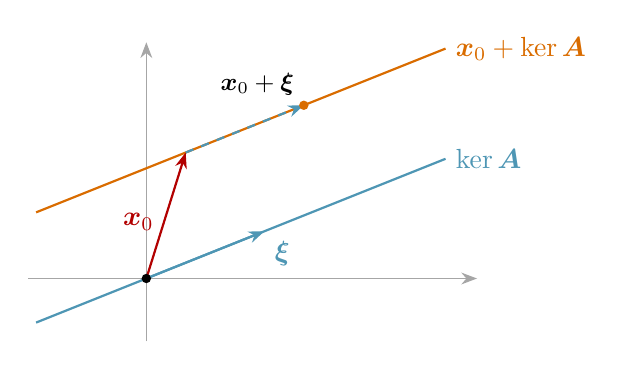
\begin{tikzpicture}
			\draw[axis] (-1.5,0) -- (4.2,0);
			\draw[axis] (0,-0.8) -- (0,3.0);
			\draw[thick,figblue] (-1.4,-0.56) -- (3.8,1.52) node[right]{$\ker\vv A$};
			\draw[thick,figorange] (-1.4,0.84) -- (3.8,2.92) node[right]{$\vv x_0+\ker\vv A$};
			\draw[vec,figred] (0,0) -- (0.5,1.6) node[pos=0.45,left]{$\vv x_0$};
			\draw[vec,figblue] (0,0) -- (1.5,0.6) node[below right]{$\vv\xi$};
			\draw[vec,figblue,dashed] (0.5,1.6) -- (2.0,2.2);
			\node[dot,figorange] at (2.0,2.2) {};
			\node[above left,font=\small] at (2.0,2.2) {$\vv x_0+\vv\xi$};
			\node[dot] at (0,0) {};
		\end{tikzpicture}
		\caption{齐次方程组的解集是过原点的子空间（蓝），非齐次方程组的解集是把它平移 $\vv x_0$ 后得到的线性流形（橙）. 改变 $\vv b$ 只改变平移量，不改变方向.}
		\label{fig:affine}
	\end{figure}
	\begin{pitfallbox}
		当 $\vv b\ne\zero$ 时，解集\textbf{不是}子空间（它不含零向量），所以谈不上``基''，也就没有``非齐次方程组的基础解系''这种说法. 通解中自由参数的个数，是方向子空间的维数 $n-r$.
	\end{pitfallbox}
	
	\subsection{方程组能确定什么}
	
	方程组有无穷多解时，并不意味着``什么都不知道''. 在第一章的物流网络中，$x_1+x_2=50$ 不论选哪个方案都成立. 一般地：
	
	\begin{theorem}[可确定性判据]\label{thm:sol-determinable}\index{ke3que4ding4xing4 pan4ju4@可确定性判据}
		设 $\vv{Ax}=\vv b$ 相容，$\vv c\in\mathbb{F}^n$. 以下条件等价：
		\begin{enumerate}
			\item 数 $\vv c^\trans\vv x$ 对所有解 $\vv x$ 取同一个值（即它被方程组\textbf{唯一确定}）；
			\item 对一切 $\vv\xi\in\ker\vv A$，$\vv c^\trans\vv\xi=0$；
			\item $\vv c^\trans$ 是 $\vv A$ 各行的线性组合；
			\item $\rk\begin{pmatrix}\vv A\\ \vv c^\trans\end{pmatrix}=\rk\vv A$.
		\end{enumerate}
	\end{theorem}
	\begin{proof}
		(1)$\Leftrightarrow$(2)：由通解结构，所有解为 $\vv x_0+\vv\xi$（$\vv\xi\in\ker\vv A$），$\vv c^\trans(\vv x_0+\vv\xi)=\vv c^\trans\vv x_0+\vv c^\trans\vv\xi$.
		
		(3)$\Leftrightarrow$(4)：添加一行不增加秩，当且仅当这一行可由原有各行线性表出.
		
		(3)$\Rightarrow$(2)：若 $\vv c^\trans=\vv y^\trans\vv A$，则 $\vv c^\trans\vv\xi=\vv y^\trans\vv{A\xi}=0$.
		
		(2)$\Rightarrow$(4)：记 $\vv A'=\begin{pmatrix}\vv A\\ \vv c^\trans\end{pmatrix}$. 由 (2)，$\vv A'\vv x=\zero\iff\vv{Ax}=\zero$，即 $\ker\vv A'=\ker\vv A$. 由秩—零化度定理，$\rk\vv A'=n-\dim\ker\vv A'=n-\dim\ker\vv A=\rk\vv A$.
	\end{proof}
	
	\begin{motivebox}
		条件 (3) 有一个朴素的解释：\textbf{能被确定的，恰好是能从已知方程``推出来''的量}——把已有方程乘上系数相加，左边恰好得到 $\vv c^\trans\vv x$，右边就是它的值. 反之，凡不能这样推出的量，都可以沿着某个 $\vv\xi\in\ker\vv A$ 的方向任意变动. 在下一节，这个判据将分别回答一个统计公开问题和一个金融定价问题.
	\end{motivebox}
	
	% ---------------------------------------------------------------------
	\section{\hC 应用：解的结构告诉我们什么}
	
	\begin{modelbox}{物流网络（续）：自由度从哪里来}
		\mstep{问题} 第一章的物流网络有两个自由变量. 这个``$2$''是巧合，还是由网络结构决定的？
		
		\mstep{求解} 用本章的语言重写第一章的结果：
		\[
		\vv x=\underbrace{\begin{pmatrix}0\\50\\0\\0\\50\end{pmatrix}}_{\text{特解}}
		+s\underbrace{\begin{pmatrix}1\\-1\\1\\0\\0\end{pmatrix}}_{\vv\xi_1}
		+t\underbrace{\begin{pmatrix}1\\-1\\0\\1\\-1\end{pmatrix}}_{\vv\xi_2}.
		\]
		特解是``全部走 $A\to C\to D$''. 基础解系的两个向量都是\textbf{环路}：$\vv\xi_1$ 沿 $A\to B\to C$ 走、再逆着 $A\to C$ 走回 $A$；$\vv\xi_2$ 沿 $A\to B\to D$ 走、再逆着 $C\to D$、$A\to C$ 回到 $A$. 在环路上加一圈流量，每个站点流入流出同时增加，平衡不受影响.
		
		\mstep{解读}
		\begin{itemize}
			\item 一般地，对有 $n$ 个站点、$m$ 条线路的连通网络，站点平衡方程的系数矩阵（称为\textbf{关联矩阵}\index{guan1lian2 ju3zhen4@关联矩阵}）的秩为 $n-1$. 因此解空间维数为 $m-(n-1)=m-n+1$，恰好是网络中\textbf{独立环路}的个数. 本例 $m=5$，$n=4$，自由度为 $2$.
			\item 由可确定性判据，$x_1+x_2$（$A$ 的总发货量）与 $x_4+x_5$（$D$ 的总收货量）被唯一确定，因为它们正是两个方程的左边；而单条线路的流量，如 $x_1$，在 $\vv\xi_1$ 上不为零，所以不被确定.
			\item 秩比方程数少 $1$，对应的就是第一章发现的守恒律``总供给 $=$ 总需求''.
		\end{itemize}
		
		\mstep{局限} 现实调度还要求流量非负、不超过线路容量，此时可行方案只是这个线性流形中的一块有界区域. 在这块区域上找成本最低的方案，是线性规划的任务.
		\begin{center}
			\begin{tikzpicture}[scale=0.8,every node/.style={transform shape}]
				\foreach \k/\dx in {1/0,2/7.2}{
					\begin{scope}[xshift=\dx cm]
						\node[station] (A\k) at (0,0) {$A$};
						\node[station] (B\k) at (2.6,1.3) {$B$};
						\node[station] (C\k) at (2.6,-1.3) {$C$};
						\node[station] (D\k) at (5.2,0) {$D$};
						\draw[vec,gray!50] (A\k) -- (B\k); \draw[vec,gray!50] (A\k) -- (C\k);
						\draw[vec,gray!50] (B\k) -- (C\k); \draw[vec,gray!50] (B\k) -- (D\k);
						\draw[vec,gray!50] (C\k) -- (D\k);
					\end{scope}
				}
				\node[sub,text width=6.2cm] at (2.6,-2.5) {(a) 环路 $\vv\xi_1$：$A\to B\to C$，再逆着 $A\to C$ 回到 $A$};
				\node[sub,text width=6.2cm] at (9.8,-2.5) {(b) 环路 $\vv\xi_2$：$A\to B\to D$，再逆着 $C\to D$、$A\to C$ 回到 $A$};
				\draw[line width=2.5pt,figred,opacity=0.55] (A1) -- (B1) node[midway,above left,opacity=1]{$+$};
				\draw[line width=2.5pt,figred,opacity=0.55] (B1) -- (C1) node[midway,right,opacity=1]{$+$};
				\draw[line width=2.5pt,figblue,opacity=0.55] (A1) -- (C1) node[midway,below left,opacity=1]{$-$};
				\draw[line width=2.5pt,figred,opacity=0.55] (A2) -- (B2) node[midway,above left,opacity=1]{$+$};
				\draw[line width=2.5pt,figred,opacity=0.55] (B2) -- (D2) node[midway,above right,opacity=1]{$+$};
				\draw[line width=2.5pt,figblue,opacity=0.55] (C2) -- (D2) node[midway,below right,opacity=1]{$-$};
				\draw[line width=2.5pt,figblue,opacity=0.55] (A2) -- (C2) node[midway,below left,opacity=1]{$-$};
			\end{tikzpicture}
			\captionof{figure}{基础解系的两个向量都是网络中的环路. 红色线路流量增加（$+$），蓝色线路流量减少（$-$），每个站点的流入流出同时变化，平衡不受影响.}
			\label{fig:cycles}
		\end{center}
	\end{modelbox}
	
	\begin{modelbox}{统计公开与隐私：汇总数据会泄露什么}
		\mstep{问题} 某地两家法院分三类案件统计结案数. 为保护当事人隐私，统计部门只公开各法院的合计（行和）与各类案件的合计（列和）：
		\begin{center}
			\begin{tabular}{c|ccc|c}
				& 民事 & 刑事 & 行政 & 合计 \\
				\hline
				法院甲 & $x_{11}$ & $x_{12}$ & $x_{13}$ & $50$ \\
				法院乙 & $x_{21}$ & $x_{22}$ & $x_{23}$ & $30$ \\
				\hline
				合计 & $40$ & $25$ & $15$ & $80$
			\end{tabular}
		\end{center}
		公众能否由公开数据反推出某个单元格？如果再公开两个单元格呢？
		
		\mstep{模型} 六个未知数满足五个方程（两个行和、三个列和）. 五个方程的系数矩阵秩为 $4$：两个行和方程之和等于三个列和方程之和. 所以解空间维数为 $6-4=2$，一组基础解系是
		\[
		\vv\xi_1:\ \begin{pmatrix}1&-1&0\\-1&1&0\end{pmatrix},\qquad
		\vv\xi_2:\ \begin{pmatrix}1&0&-1\\-1&0&1\end{pmatrix}
		\]
		（这里把六个分量排成表格的样子）. 它们的行和与列和都为零.
		
		\mstep{求解}
		\begin{itemize}
			\item 单元格 $x_{11}$ 能否确定？取 $\vv c$ 为 $x_{11}$ 处为 $1$、其余为 $0$ 的向量，则 $\vv c^\trans\vv\xi_1=1\ne0$. 由可确定性判据，\textbf{不能确定}. 只公开边际合计时，单个单元格是安全的.
			\item 若再公开 $x_{11}=28$，$x_{12}=15$：方向子空间中的向量 $a\vv\xi_1+b\vv\xi_2$ 必须满足 $a+b=0$（$x_{11}$ 方向）与 $-a=0$（$x_{12}$ 方向），得 $a=b=0$. 解空间变为零维，\textbf{全表被唯一确定}：$x_{13}=7$，$x_{21}=12$，$x_{22}=10$，$x_{23}=8$.
		\end{itemize}
		
		\mstep{解读} 公开两个``看似无害''的单元格，配合边际合计，就泄露了整张表. 这正是统计机构在发布数据前要做\textbf{单元格抑制}\index{dan1yuan2ge2 yi4zhi4@单元格抑制}（隐藏部分单元格）时必须考虑的问题：不能只隐藏敏感单元格本身，还要保证它不能被其余公开数据``线性推出''. 判断标准正是定理~\ref{thm:sol-determinable}.
		
		\mstep{局限} 真实数据中，计数是非负整数. 即使一个单元格不能被唯一确定，结合非负性也可能把它限制在很小的范围内（例如 $0\le x_{13}\le15$），同样构成泄露风险. 这类分析需要整数规划等工具，是统计披露控制领域的研究内容.
	\end{modelbox}
	
	\begin{modelbox}{一价定律与状态价格（接第二章``复制组合''）}
		\mstep{问题} 第二章的市场有三种状态、三种资产（债券 $\vv b$、股票 $\vv s$、看涨期权 $\vv c$）. 现在又上市了一只基金 $\vv f=(4,2,1)^\trans$. 已知 $\vv b,\vv s,\vv c$ 的价格分别为 $0.95$，$1.2$，$0.6$ 元，基金应该卖多少钱？
		
		\mstep{模型} 以四种资产的收益为列，作收益矩阵
		\[\vv S=\begin{pmatrix}1&3&2&4\\1&1&0&2\\1&0&0&1\end{pmatrix}.\]
		持有份额为 $\vv k\in\mathbb{R}^4$ 的组合，收益为 $\vv{Sk}$，成本为 $\vv p^\trans\vv k$，其中 $\vv p$ 是价格向量.
		
		\mstep{求解} $\rk\vv S=3$，$\ker\vv S$ 是一维的，由 $\vv\xi=(1,1,0,-1)^\trans$ 张成：``买一份债券、一份股票，卖一份基金''，收益在每种状态下都是零.
		\begin{itemize}
			\item 能复制某个收益 $\vv y$ 的组合，是 $\vv{Sk}=\vv y$ 的全部解 $\vv k_0+t\vv\xi$. 它们收益相同，所以必须同价（\textbf{一价定律}\index{yi1jia4 ding4lv4@一价定律}），即 $\vv p^\trans\vv\xi=0$：$p_f=p_b+p_s=2.15$ 元.
			\item 由可确定性判据，一价定律成立当且仅当 $\vv p^\trans$ 是 $\vv S$ 各行的线性组合，即存在 $\vv q\in\mathbb{R}^3$ 使 $\vv p^\trans=\vv q^\trans\vv S$. 解得 $\vv q=(0.3,0.3,0.35)^\trans$.
		\end{itemize}
		
		\mstep{解读}
		\begin{itemize}
			\item $q_i$ 是``只在第 $i$ 种状态支付 $1$ 元''的证券的价格，称为\textbf{状态价格}\index{zhuang4tai4 jia4ge2@状态价格}. $q_1=0.3$ 正是第二章算出的``繁荣险''价格——两种方法给出了同一个答案.
			\item 若市场上基金卖 $2.20$ 元，就可以买入债券和股票（花 $2.15$ 元），同时卖出基金（收 $2.20$ 元）. 未来无论哪种状态，收益都相互抵消，却白赚 $0.05$ 元. 这就是\textbf{套利}. 套利者的买卖会推动价格回到 $2.15$ 元.
			\item 一价定律说的是``价格是收益的线性函数''；状态价格就是这个线性函数在标准基下的坐标.
		\end{itemize}
		
		\mstep{局限} 本例的状态价格恰好都为正. 金融学中更强的``无套利''条件要求状态价格\textbf{严格为正}，证明它需要处理不等式的工具（Farkas 引理、线性规划对偶），超出了线性方程组的范围.
	\end{modelbox}
	
	\begin{modelbox}{当方程比未知量多：最小二乘的序幕}
		\mstep{问题} 某商品四个季度的广告投入 $x$（万元）与销售额 $y$（十万元）为 $(1,2)$，$(2,3)$，$(3,5)$，$(4,6)$. 用直线 $y=a+bx$ 描述二者的关系，$a,b$ 应取多少？
		
		\mstep{模型} 要求直线经过四个点，就是解关于 $a,b$ 的方程组
		\[\vv A\begin{pmatrix}a\\b\end{pmatrix}=\vv y,\qquad
		\vv A=\begin{pmatrix}1&1\\1&2\\1&3\\1&4\end{pmatrix},\quad\vv y=\begin{pmatrix}2\\3\\5\\6\end{pmatrix}.\]
		
		\mstep{求解} 对增广矩阵消元可得 $\rk\vv A=2$，$\rk(\vv A\mid\vv y)=3$. 由定理~\ref{thm:rouche}，方程组\textbf{无解}：没有一条直线同时穿过四个点. 由推论~\ref{cor:sol-fullrank}，$\vv A$ 列满秩，所以即使有解也至多一个；困难只在于存在性.
		
		\mstep{解读} 这不是模型错了，而是问题问错了. 观测数据总带有误差，数据点多于参数时，方程组几乎总是不相容的. 正确的问题不是``哪条直线\textbf{恰好}过所有点''，而是``哪条直线\textbf{最接近}所有点''. 回答它需要``距离''和``垂直''的概念——这正是第九章内积空间的出发点. 届时我们会求出最佳直线 $y=0.5+1.4x$.
	\end{modelbox}
	
	% ---------------------------------------------------------------------
	\section{ 矩阵方程与秩不等式}
	
	\subsection{矩阵方程 \texorpdfstring{$\vv{AX}=\vv B$}{AX=B}}
	
	设 $\vv A$ 为 $m\times n$ 矩阵，$\vv B$ 为 $m\times p$ 矩阵. 求 $n\times p$ 矩阵 $\vv X$ 使 $\vv{AX}=\vv B$. 按列分块，$\vv{AX}=\vv B$ 等价于 $p$ 个方程组 $\vv A\vv x_j=\vv b_j$（$j=1,\ldots,p$），它们共用同一个系数矩阵. 所以只需对 $(\vv A\mid\vv B)$ 一次性做初等行变换，同时求解. 求逆矩阵的 $(\vv A\mid\vv I)$ 方法正是 $\vv B=\vv I$ 的特例.
	
	\begin{proposition}
		$\vv{AX}=\vv B$ 有解，当且仅当 $\rk\vv A=\rk(\vv A\mid\vv B)$.
	\end{proposition}
	\begin{proof}
		有解 $\iff$ $\vv B$ 的每一列都可由 $\vv A$ 的列线性表出 $\iff$ $\vv A$ 与 $(\vv A\mid\vv B)$ 的列向量组等价 $\iff$ 二者秩相等（论证同定理~\ref{thm:rouche}）.
	\end{proof}
	
	\begin{example}
		解 $\begin{pmatrix}1&1\\1&2\end{pmatrix}\vv X=\begin{pmatrix}1&0&3\\2&1&5\end{pmatrix}$.
	\end{example}
	\begin{solution}
		\[
		\left(\begin{NiceArray}{cc:ccc}1&1&1&0&3\\1&2&2&1&5\end{NiceArray}\right)
		\xrightarrow{r_2-r_1}
		\left(\begin{NiceArray}{cc:ccc}1&1&1&0&3\\0&1&1&1&2\end{NiceArray}\right)
		\xrightarrow{r_1-r_2}
		\left(\begin{NiceArray}{cc:ccc}1&0&0&-1&1\\0&1&1&1&2\end{NiceArray}\right),
		\]
		故 $\vv X=\begin{pmatrix}0&-1&1\\1&1&2\end{pmatrix}$. 可以直接验证 $\vv{AX}$ 等于右端.
	\end{solution}
	
	\subsection{秩不等式}
	
	第三章证明了 $\rk(\vv{AB})\le\min\{\rk\vv A,\rk\vv B\}$，这是秩的上界. 解空间的维数给出了一个下界.
	
	\begin{theorem}[Sylvester 不等式]\label{thm:sylvester}\index{sylvester bu4deng3shi4@Sylvester 不等式}
		设 $\vv A$ 为 $m\times n$ 矩阵，$\vv B$ 为 $n\times p$ 矩阵，则
		\[\rk(\vv{AB})\ge\rk\vv A+\rk\vv B-n.\]
	\end{theorem}
	\begin{proof}
		把 $\vv A$ 看作线性映射 $\mathbb{F}^n\to\mathbb{F}^m$，限制在子空间 $\imm\vv B$ 上. 这个限制映射的像是 $\vv A(\imm\vv B)=\imm(\vv{AB})$，核是 $\ker\vv A\cap\imm\vv B$. 对它用秩—零化度定理：
		\[
		\begin{aligned}
			\rk\vv B=\dim\imm\vv B&=\rk(\vv{AB})+\dim(\ker\vv A\cap\imm\vv B)\\
			&\le\rk(\vv{AB})+\dim\ker\vv A\\
			&=\rk(\vv{AB})+n-\rk\vv A.
		\end{aligned}
		\]
		移项即得.
	\end{proof}
	
	Sylvester 不等式的另一个证明见第三章练习.
	
	\begin{motivebox}
		先做 $\vv B$、再做 $\vv A$，``信息''会在两处丢失：$\vv B$ 本身的降秩，以及 $\vv B$ 的像中落进 $\ker\vv A$ 而被 $\vv A$ 压扁的部分. 后者至多是 $\dim\ker\vv A=n-\rk\vv A$ 维，这就是不等式中 $-n$ 的来源.
	\end{motivebox}
	
	\begin{corollary}
		\begin{enumerate}
			\item 若 $\vv{AB}=\vv O$，则 $\rk\vv A+\rk\vv B\le n$.
			\item 若 $\vv A$ 为 $n$ 阶方阵且 $\vv A^2=\vv O$，则 $\rk\vv A\le n/2$.
		\end{enumerate}
	\end{corollary}
	\begin{proof}
		(1) 在 Sylvester 不等式中令 $\rk(\vv{AB})=0$. (2) 在 (1) 中取 $\vv B=\vv A$.
	\end{proof}
	
	推论 (1) 也可以直接看出：$\vv{AB}=\vv O$ 说明 $\vv B$ 的每一列都是 $\vv{Ax}=\zero$ 的解，所以 $\rk\vv B\le\dim\ker\vv A=n-\rk\vv A$.
	
	% ---------------------------------------------------------------------
	\section{*消元法的矩阵形式：LU 分解（选读）}
	
	\subsection{LU 分解}
	
	在第一章的消元过程中，如果\textbf{不需要交换行}，我们只用到第三类初等变换 $r_i+cr_j$（$i>j$，即用上面的行去消下面的行）. 对应的初等矩阵 $\vv E(i,j(c))$ 是对角元全为 $1$ 的下三角矩阵，称为\textbf{单位下三角矩阵}\index{dan1wei4 xia4 san1jiao3 ju3zhen4@单位下三角矩阵}.
	
	\begin{lemma}
		单位下三角矩阵的乘积仍是单位下三角矩阵；单位下三角矩阵可逆，其逆也是单位下三角矩阵.
	\end{lemma}
	
	证明留作练习. 于是若 $\vv E_k\cdots\vv E_1\vv A=\vv U$ 为上三角矩阵，则
	\[\vv A=(\vv E_k\cdots\vv E_1)^{-1}\vv U=\vv L\vv U,\]
	其中 $\vv L$ 是单位下三角矩阵.
	
	\begin{theorem}[LU 分解]\label{thm:lu}\index{lu fen1jie3@LU 分解}
		若方阵 $\vv A$ 用消元法化为上三角形的过程中不需要交换行，则 $\vv A=\vv{LU}$，其中 $\vv L$ 为单位下三角矩阵，$\vv U$ 为上三角矩阵. 进一步可以验证：$\vv L$ 的 $(i,j)$ 元（$i>j$）恰好是消元时``第 $i$ 行减去第 $j$ 行的倍数''.
	\end{theorem}
	
	\begin{example}
		对 $\vv A=\begin{pmatrix}2&1&1\\4&3&3\\8&7&9\end{pmatrix}$ 做消元：$r_2-2r_1$，$r_3-4r_1$，再 $r_3-3r_2$，得
		\[
		\vv U=\begin{pmatrix}2&1&1\\0&1&1\\0&0&2\end{pmatrix},\qquad
		\vv L=\begin{pmatrix}1&0&0\\2&1&0\\4&3&1\end{pmatrix}.
		\]
		$\vv L$ 中的 $2,4,3$ 正是三次消元的倍数. 可以直接验证 $\vv{LU}=\vv A$.
	\end{example}
	
	\paragraph*{为什么要分解.} 有了 $\vv A=\vv{LU}$，解 $\vv{Ax}=\vv b$ 分两步：先由 $\vv{Ly}=\vv b$ 自上而下求 $\vv y$（\textbf{前代}\index{qian2dai4@前代}），再由 $\vv{Ux}=\vv y$ 自下而上求 $\vv x$（\textbf{回代}\index{hui2dai4@回代}）. 对 $n$ 阶矩阵，分解本身约需 $\frac23n^3$ 次运算，而每次前代加回代只需约 $2n^2$ 次. 当同一个 $\vv A$ 要配上\textbf{许多个不同的} $\vv b$ 时，分解一次、反复使用，能节省大量计算.
	
	\begin{linkbox}{投入产出的情景分析}
		第一部分综合项目一要求分析``某部门最终需求下降 $10\%$''的影响. 实际工作中，分析人员往往要试验几十上百种需求情景 $\vv d$，而系数矩阵 $\vv I-\vv A$ 始终不变. 对 $\vv I-\vv A$ 做一次 LU 分解，每种情景只需一次前代和回代. 投入产出表有上百个部门时，这比每次重新消元快得多，也比先求出整个逆矩阵更省计算、数值上更稳定.
	\end{linkbox}
	
	\begin{remark}
		消元中若遇到零主元，就必须交换行. 此时一般有 $\vv{PA}=\vv{LU}$，其中 $\vv P$ 是若干对换矩阵的乘积（称为\textbf{置换矩阵}\index{zhi4huan4 ju3zhen4@置换矩阵}）. 数值计算软件为了减小舍入误差，即使主元不为零，也常常主动选取绝对值最大的元素作主元（\textbf{列主元消元法}\index{lie4 zhu3yuan2 xiao1yuan2fa3@列主元消元法}）.
	\end{remark}
	
	\subsection{病态方程组}
	
	\begin{example}
		比较两个方程组
		\[
		\left\{\begin{array}{l}x+y=2,\\x+1.0001y=2.0001,\end{array}\right.\qquad
		\left\{\begin{array}{l}x+y=2,\\x+1.0001y=2.0002.\end{array}\right.
		\]
		第一个的解是 $(1,1)$；第二个只把一个常数改动了万分之一，解却变成了 $(0,2)$.
	\end{example}
	
	两条直线几乎平行，交点的位置对数据的微小扰动极其敏感. 这样的方程组称为\textbf{病态}\index{bing4tai4@病态（方程组）}的. 当系数来自测量、统计或估计（例如投入产出表中的消耗系数）时，病态意味着\textbf{数据中的误差会被成倍放大到结果里}，算得再精确也没有意义.
	\begin{figure}[htbp]
		\centering
		\begin{tikzpicture}[scale=0.8]
			\draw[axis] (-0.3,0) -- (8.6,0);
			\draw[axis] (0,-0.9) -- (0,3.0);
			\draw[thick,figblue] (0,0) -- (8.4,2.52);
			\draw[thick,figorange] (0,-0.4) -- (8.4,2.792);
			\draw[thick,figorange,dashed] (0,-0.6) -- (8.4,2.592);
			\node[dot,figred] at (5,1.5) {};
			\node[dot,figred] at (7.5,2.25) {};
			\node[figred,above left,font=\small] at (5,1.5) {原来的解};
			\node[figred,below right,font=\small] at (7.5,2.25) {扰动后的解};
			\draw[decorate,decoration={brace,amplitude=3pt,mirror}] (0.15,-0.62) -- (0.15,-0.38);
			\node[right,font=\small] at (0.35,-0.75) {常数项的微小改变};
		\end{tikzpicture}
		\caption{两条几乎平行的直线（图中有意夸大了夹角）. 一条直线稍一平移，交点就沿着另一条直线跑出很远：这就是病态.}
		\label{fig:illcond}
	\end{figure}
	\begin{pitfallbox}
		行列式很小，并\textbf{不}说明方程组病态. 把上例第一个方程组的两边都乘以 $1000$，行列式变为原来的 $10^6$ 倍，但解对扰动的敏感程度丝毫未变；反之，$\vv A=0.001\vv I_{10}$ 的行列式是 $10^{-30}$，方程组却毫不病态. 衡量病态程度的正确工具是\textbf{条件数}\index{tiao2jian4shu4@条件数}，它需要``向量的长度''（范数），将在第九章之后介绍.
	\end{pitfallbox}
	
	\begin{historybox}{名字与概念}
		\sidefig[0.25\linewidth]{image/frobenius.jpg}{弗罗贝尼乌斯}[fig:frobenius]
		``有解当且仅当系数矩阵与增广矩阵的秩相等''这一定理，在不同国家的教材中有不同的名字：法语、意大利语、西班牙语文献多称 Rouché–Capelli 定理，俄语文献则称 Kronecker–Capelli 定理. 名字不同，是因为 19 世纪后期多位数学家各自独立地得到了等价的结论\cite{rouche1875discussion}. ``秩''作为一个独立的概念，通常归功于德国数学家弗罗贝尼乌斯（F.~G.~Frobenius）\cite{frobenius1879homogene}. 一个定理的``归属''往往比它本身复杂得多.
	\end{historybox}
	
	\begin{codebox}{从简化阶梯形到通解}
		\mstep{目标} 让程序自动写出``特解 $+$ 基础解系''形式的通解，并用它重看物流网络的两个环路.
		
		\mstep{准备} 第一章写的 \texttt{rref(M)}；用于对照的 \texttt{scipy.linalg.null\_space} 与 \texttt{numpy.linalg.matrix\_rank}.
		
		\mstep{任务}
		\begin{enumerate}
			\item 写函数 \texttt{null\_basis(A)}：依次令一个自由变量取 $1$、其余取 $0$，解出主变量，返回基础解系.
			\item 写函数 \texttt{particular(M)}：对增广矩阵 $\vv M$，令全部自由变量取 $0$，求出一个特解；无解时返回 \texttt{None}.
			\item 用第一章第二个例题检验两个函数，再随机取几组 $k_1,k_2$，验证 $\vv x_0+k_1\vv\xi_1+k_2\vv\xi_2$ 都是解.
			\item 对物流网络重复任务 3.
			\item \texttt{scipy.linalg.null\_space} 给出的是另一组基. 把两组基并排拼成一个矩阵，用秩说明它们张成同一个子空间.
		\end{enumerate}
		
		\mstep{检查点} 第一章例题：$\vv\xi_1=(-2,1,0,0)^\trans$，$\vv\xi_2=(-2,0,-1,1)^\trans$，$\vv x_0=(3,0,2,0)^\trans$. 物流网络：$\vv x_0=(0,50,0,0,50)^\trans$，基础解系为 $(1,-1,1,0,0)^\trans$ 与 $(1,-1,0,1,-1)^\trans$，与正文的两个环路一致. 任务 5 中拼起来的矩阵秩为 $2$.
		
		\mstep{思考}
		\begin{enumerate}
			\item 基础解系不唯一，但其中向量的个数总是 $n-\rk\vv A$. 你的程序在哪一行代码里``体现''了这个数？
			\item 如果特解改为令自由变量取 $1$ 而不是 $0$，通解的写法变了，解集变了吗？
		\end{enumerate}
	\end{codebox}
	
	\section{*纠错码：Hamming 码（选读）}\label{sec:hamming}
	
	数据在存储和传输中会出错：内存中的一位可能被宇宙射线翻转，信号可能被噪声干扰. 一个朴素的办法是把每一位重复三遍，按多数表决纠正一位错误，但这样要用三倍的存储. 1950 年汉明（R.~W.~Hamming）给出了一种只用 $7$ 位传送 $4$ 位数据、同样能纠正任意一位错误的方法\cite{hamming1950error}. 它的全部原理，是一个齐次线性方程组的解空间——只不过方程组的系数和未知数只取 $0$ 和 $1$.
	
	\subsection{二进制域}
	
	计算机里的数据是由 $0$ 和 $1$ 组成的串. 在集合 $\{0,1\}$ 上按``模 $2$''定义加法与乘法：
	\[
	0+0=0,\quad 0+1=1+0=1,\quad 1+1=0;\qquad 0\cdot0=0\cdot1=1\cdot0=0,\quad 1\cdot1=1.
	\]
	加法就是``异或''：两位相同得 $0$，不同得 $1$. 注意 $1+1=0$，所以 $-1=1$，减法与加法相同. 记这个数系为 $\mathbb{F}_2$.
	
	$\mathbb{F}_2$ 不是第二章定义的数域——它不是复数集的子集. 但第二章数域定义中真正用到的只是：加、减、乘、除（除数非零）可以进行，并且满足通常的运算律. 满足这些条件的数系称为\textbf{域}\index{yu4@域}(field)，$\mathbb{F}_2$ 是只有两个元素的域. 第一至六章的定义与定理，凡是只用到四则运算的——消元法、线性相关、基与维数、秩、基础解系——在任何域上都成立. 本节就在 $\mathbb{F}_2$ 上使用它们. 第二章章末习题 C5 已经在 $\mathbb{F}_2^3$ 中数过向量和子空间.
	
	\begin{pitfallbox}
		在 $\mathbb{F}_2$ 上，``$\vv x\neq\zero$ 时 $\vv x^\trans\vv x>0$''不再成立：$(1,1)^\trans$ 与自身的``内积''是 $1+1=0$. 依赖于大小比较、开方或``平方和为零则全为零''的结论（第九章以后的内积、长度、正交投影）都不能照搬到 $\mathbb{F}_2$ 上.
	\end{pitfallbox}
	
	\subsection{校验矩阵与码字}
	
	设
	\[
	\vv H=\begin{pmatrix}
		1&0&1&0&1&0&1\\
		0&1&1&0&0&1&1\\
		0&0&0&1&1&1&1
	\end{pmatrix}.
	\]
	它的第 $j$ 列，从上往下读，恰好是 $j$ 的二进制表示的低位到高位（例如第 $6$ 列是 $(0,1,1)^\trans$，$6=0\cdot1+1\cdot2+1\cdot4$）. 七个列两两不同，且都不是零向量.
	
	\begin{definition}
		称 $\mathbb{F}_2^7$ 中满足 $\vv H\vv x=\zero$ 的向量为\textbf{码字}\index{ma3zi4@码字}(codeword)，全体码字构成的子空间 $C=\ker\vv H$ 称为 $(7,4)$ \textbf{Hamming 码}\index{hamming ma3@Hamming 码}，$\vv H$ 称为它的\textbf{校验矩阵}\index{jiao4yan4 ju3zhen4@校验矩阵}(parity-check matrix).
	\end{definition}
	
	$\vv H$ 的第 $1,2,4$ 列构成单位矩阵，所以 $\rk\vv H=3$. 由定理~\ref{thm:sol-homog}（在 $\mathbb{F}_2$ 上同样成立），$\dim C=7-3=4$，$C$ 恰有 $2^4=16$ 个码字. 把 $x_1,x_2,x_4$ 取为主元变量，方程组 $\vv H\vv x=\zero$ 化为（注意减法即加法）
	\[
	x_1=x_3+x_5+x_7,\qquad x_2=x_3+x_6+x_7,\qquad x_4=x_5+x_6+x_7.
	\]
	自由变量 $x_3,x_5,x_6,x_7$ 依次取单位向量，得到一组基础解系
	\[
	\begin{aligned}
		\vv g_1&=(1,1,1,0,0,0,0)^\trans, & \vv g_2&=(1,0,0,1,1,0,0)^\trans,\\
		\vv g_3&=(0,1,0,1,0,1,0)^\trans, & \vv g_4&=(1,1,0,1,0,0,1)^\trans.
	\end{aligned}
	\]
	以它们为列的 $7\times4$ 矩阵 $\vv G$ 称为\textbf{生成矩阵}\index{sheng1cheng2 ju3zhen4@生成矩阵}(generator matrix)，满足 $\vv H\vv G=\vv O$.
	
	\paragraph*{编码.} 要发送的 $4$ 位数据 $\vv d=(d_1,d_2,d_3,d_4)^\trans$ 编码为码字 $\vv c=\vv G\vv d$. 这相当于把数据放在第 $3,5,6,7$ 位，再按上面三个等式算出第 $1,2,4$ 位的\textbf{校验位}. 例如数据 $(1,0,1,1)$ 编码为
	\[
	\vv c=\vv g_1+\vv g_3+\vv g_4=(0,1,1,0,0,1,1)^\trans.
	\]
	
	\subsection{伴随式与纠错}
	
	设发送的是码字 $\vv c$，收到的是 $\vv r=\vv c+\vv e$，其中 $\vv e$ 记录了哪些位出错（出错的位为 $1$）. 接收方不知道 $\vv c$ 和 $\vv e$，但可以计算
	\[
	\vv s=\vv H\vv r=\vv H\vv c+\vv H\vv e=\vv H\vv e,
	\]
	称为\textbf{伴随式}\index{ban4sui2shi4@伴随式}(syndrome，也译作校正子). 它只与错误有关，与发送了什么无关.
	
	若没有出错，$\vv s=\zero$. 若只有第 $j$ 位出错，$\vv e$ 是第 $j$ 个标准单位向量，$\vv s=\vv H\vv e$ 就是 $\vv H$ 的第 $j$ 列——也就是 $j$ 的二进制表示. 七个列两两不同，所以\textbf{伴随式直接指出了出错的位置}，把那一位翻转即可纠正.
	
	\begin{example}
		发送上面的码字 $\vv c=(0,1,1,0,0,1,1)^\trans$，第 $5$ 位出错，收到 $\vv r=(0,1,1,0,1,1,1)^\trans$. 计算
		\[
		\vv s=\vv H\vv r=(1,0,1)^\trans,
		\]
		它是 $\vv H$ 的第 $5$ 列（$1\cdot1+0\cdot2+1\cdot4=5$）. 翻转第 $5$ 位，恢复 $\vv c$，再从第 $3,5,6,7$ 位读出数据 $(1,0,1,1)$.
		
		若第 $1,2$ 两位同时出错，则 $\vv s$ 是第 $1,2$ 列之和 $(1,1,0)^\trans$，即第 $3$ 列. 接收方会``纠正''第 $3$ 位，结果错了三位. Hamming 码只保证纠正一位错误.
	\end{example}
	
	\begin{remark}
		``伴随式''与第五章的``伴随矩阵''只是中文译名相同，二者没有关系.
	\end{remark}
	
	\begin{figure}[htbp]
		\centering
		\begin{tikzpicture}[scale=1.15]
			\draw[thick,figblue]   (-0.6,0.35) circle (1.1);
			\draw[thick,figorange] (0.6,0.35)  circle (1.1);
			\draw[thick,figgreen]  (0,-0.6)    circle (1.1);
			\node[font=\small] at (-1.2,0.7)  {$x_1$};
			\node[font=\small] at (1.2,0.7)   {$x_2$};
			\node[font=\small] at (0,-1.25)   {$x_4$};
			\node[font=\small] at (0,0.85)    {$x_3$};
			\node[font=\small] at (-0.65,-0.35) {$x_5$};
			\node[font=\small] at (0.65,-0.35)  {$x_6$};
			\node[font=\small] at (0,0.03)    {$x_7$};
			\node[figblue,font=\small]   at (-1.75,1.4) {第 1 行};
			\node[figorange,font=\small] at (1.75,1.4)  {第 2 行};
			\node[figgreen,font=\small]  at (1.25,-1.5) {第 3 行};
		\end{tikzpicture}
		\caption{$\vv H$ 的三行对应三个圆，每个圆包含该行中为 $1$ 的四个位置. $\vv H\vv x=\zero$ 即每个圆内 $1$ 的个数为偶数. 一位出错时，恰好是包含它的那些圆变``奇''，而七个区域被圆覆盖的方式各不相同.}
		\label{fig:hamming-venn}
	\end{figure}

	两个等长的 $0$-$1$ 串中不同位的个数称为它们的 \textbf{Hamming 距离}\index{hamming ju4li2@Hamming 距离}，记为 $d(\vv x,\vv y)$. 在 $\mathbb{F}_2$ 上，$\vv x$ 与 $\vv y$ 不同的位正是 $\vv x+\vv y$ 中为 $1$ 的位，所以 $d(\vv x,\vv y)$ 等于 $\vv x+\vv y$ 中 $1$ 的个数.
	
	\begin{proposition}
		Hamming 码中任意两个不同码字的距离至少为 $3$，并且存在距离恰为 $3$ 的码字.
	\end{proposition}
	\begin{proof}
		$C$ 是子空间，两个码字之和仍是码字，所以只需证明：非零码字中至少有三个 $1$. 若码字 $\vv c$ 只有第 $j$ 位为 $1$，则 $\vv H\vv c$ 是 $\vv H$ 的第 $j$ 列，不为零；若只有第 $i,j$ 位为 $1$，则 $\vv H\vv c$ 是第 $i,j$ 列之和，因两列不同而不为零. 二者都与 $\vv H\vv c=\zero$ 矛盾. 另一方面，$\vv g_1$ 恰有三个 $1$.
	\end{proof}
	
	用线性相关的语言说：$\vv H$ 的任意两列线性无关，而存在三列线性相关. 码字之间至少隔开 $3$ 位，所以一个码字错一位后，仍然离它最近，而与其他码字至少相距 $2$——``就近还原''不会出错.
	
	还有更巧的事：每个码字连同与它距离为 $1$ 的 $7$ 个向量共 $8$ 个，$16$ 个码字的这些``邻域''两两不交，总数 $16\times8=128=2^7$，恰好铺满整个 $\mathbb{F}_2^7$. 也就是说，任何收到的串都恰好落在某个码字的邻域里，没有一点浪费. 具有这种性质的码称为\textbf{完美码}\index{wan2mei3 ma3@完美码}(perfect code).
	
	\subsection{实际的纠错码}
	
	码率 $4/7$ 意味着约 $57\%$ 的存储用于数据，而三重重复码只有 $1/3$. 在 $\vv H$ 下方添一行全 $1$、右边添一列，得到 $(8,4)$ 扩展 Hamming 码，它能纠正一位错误，同时发现（但不能纠正）两位错误，服务器内存中的 ECC 校验就基于这一思想. 二维码、光盘、深空通信使用的纠错码（如 Reed–Solomon 码）更强，它们在更大的有限域上构造，用到第七章的多项式（参见第七章章末习题 C8）. 研究这些码的学科称为\textbf{编码理论}，是\textbf{纠错码}\index{jiu1cuo4 ma3@纠错码}与通信工程的基础.
	
	\begin{linkbox}{校验码不是哈希值}
		电子证据保全中常用``哈希值''核对文件是否被改动. 二者目的不同：纠错码是线性的、公开的，任何人都能为改动后的数据重新算出合法的校验位，它只防\textbf{无意}的错误；密码学哈希函数被设计成非线性的、难以伪造，用来发现\textbf{有意}的篡改. 正因为 Hamming 码是线性的，它才能用一个矩阵乘法完成纠错；也正因为是线性的，它不能用来证明数据未被篡改.
	\end{linkbox}
		
	% ---------------------------------------------------------------------
	\newpage
	\ExSolutions
	
	\chapter*{第一部分综合项目}
	\addcontentsline{toc}{chapter}{第一部分综合项目}
	\markboth{第一部分综合项目}{第一部分综合项目}
	
	\paragraph*{要求.} 3—4 人一组，在下面三个项目中任选其一，两到三周完成. 提交不超过 8 页的报告（另附代码与数据），报告须包含``问题—假设—模型—求解—解读—局限''六个部分；``局限''一节与计算结果同等重要. 代码须能由他人在说明的环境中重新运行，得到报告中的全部数字与图表. 评分按本部分所附量规进行，第二、三部分的综合项目使用同一量规.
	
	\section*{项目一：一张真实的投入产出表}
	\begin{enumerate}
		\item 从国家统计局公开发布的全国投入产出表中选取最近一期，把部门合并为 6—10 个，并说明合并的理由.
		\item 计算直接消耗系数矩阵 $\vv A$，检验 Hawkins–Simon 条件.
		\item 计算列昂惕夫逆矩阵与各部门产出乘数，找出关联度最高的三个部门，并结合经济常识解释.
		\item 情景分析：若某部门的最终需求下降 $10\%$，各部门总产出如何变化？哪个部门受到的间接冲击最大？
		\item 讨论：固定系数假设在你选的数据年份到今天之间是否仍然合理？
	\end{enumerate}
	
	\section*{项目二：一个小型引证网络}
	\begin{enumerate}
		\item 在某一法律领域中选取 20—30 份公开的裁判文书或学术论文，人工标注引用关系，建立邻接矩阵. 说明你的选择标准与标注规则.
		\item 检验网络是否无环，计算 $\vv A^k$ 并找出最长的引证链条.
		\item 用被引次数排序，并与你（或法学专业同学）的直觉判断比较，列出不一致之处.
		\item 讨论：否定性引用应当如何建模？保留这个问题，第八章将给出一种回答.
	\end{enumerate}
	
	\section*{项目三：法条检索原型}
	\begin{enumerate}
		\item 选取一部法律的 50 条左右条文，手工或用分词工具确定 100 个左右关键词，建立词项—文档矩阵.
		\item 设计 5 个模拟案情查询，用 $\vv A^\trans\vv q$ 打分，评价排名前五的结果是否合理.
		\item 找出``共同词数''打分的至少两个缺陷（例如长条文天然得分高），提出改进思路. 第九章的余弦相似度是其中一种答案.
	\end{enumerate}
	
	\begin{note}
		使用公开数据时，请遵守数据来源网站的使用条款，并在报告中注明来源.
	\end{note}
	
	\section*{评分量规}\phantomsection\label{sec:rubric}
	
	三个部分的综合项目都按下表评分，满分 $100$ 分. 每一维度先判断达到哪一档，再在该档的分数范围内给分. 各项目另有若干``检查点''（见各项目末尾或下文），检查点未完成的，``模型与数学正确性''一项不得进入``优秀''档.
	
	{\small\setlength{\tabcolsep}{3pt}
			\begin{longtable}{>{\raggedright\arraybackslash}p{0.13\linewidth}p{0.05\linewidth}*{4}{>{\raggedright\arraybackslash}p{0.175\linewidth}}}
			\toprule
			维度 & 分值 & 优秀 & 良好 & 合格 & 不合格 \\
			\midrule
			\endfirsthead
			\toprule
			维度 & 分值 & 优秀 & 良好 & 合格 & 不合格 \\
			\midrule
			\endhead
			\bottomrule
			\endfoot
			问题与数据 & 15 & 问题表述清楚，数据来源可追溯，数据处理（如部门合并、关键词选择）的理由充分 & 问题与数据来源清楚，处理理由基本充分 & 说明了数据来源，处理过程交代不全 & 数据来源不明，或问题与数据脱节 \\
			\addlinespace
			模型与数学正确性 & 25 & 模型与问题匹配，所用定理的条件逐一核对，计算无误，能用书中的结论解释每一步 & 模型合理，计算基本无误，个别定理条件未核对 & 模型可用，有不影响结论的计算错误 & 模型与问题不符，或有影响结论的错误 \\
			\addlinespace
			计算与可复现性 & 20 & 代码结构清楚、有注释，一条命令即可重现全部结果，并做了交叉验证（如精确算法与数值算法对照） & 代码可运行并重现主要结果 & 代码需手工修改才能运行，或只能重现部分结果 & 无代码，或结果不可重现 \\
			\addlinespace
			解读 & 15 & 把数学结论翻译回专业语言，指出结论对决策的含义，并与常识或文献比较 & 解读准确，与专业问题有联系 & 只复述计算结果，解读较少 & 解读错误或缺失 \\
			\addlinespace
			局限与反思 & 15 & 具体指出模型在哪些假设下失效、失效会怎样影响结论，并提出可行的改进 & 指出了主要假设的局限 & 局限的讨论泛泛而谈 & 没有讨论局限 \\
			\addlinespace
			表达与规范 & 10 & 结构清楚，图表规范、有标题与单位，引用规范，注明数据使用条款 & 表达清楚，有少量格式问题 & 表达尚可，图表或引用不规范 & 难以阅读，或有未注明来源的引用 \\
		\end{longtable}
	}
	\newpage
	\paragraph*{检查点.}
	\begin{itemize}
		\item 项目一：报告直接消耗系数矩阵与列昂惕夫逆矩阵；验证 $(\vv I-\vv A)(\vv I-\vv A)^{-1}=\vv I$；说明 Hawkins–Simon 条件是否成立.
		\item 项目二：给出邻接矩阵与标注规则；说明网络是否无环，并与 $\vv A$ 是否幂零相互印证.
		\item 项目三：给出词项—文档矩阵的规模与稀疏程度；至少一个查询给出完整的打分表.
	\end{itemize}
	
	\paragraph*{小组分工.} 报告末尾附一段分工说明. 教师可以根据分工说明与答辩表现，在小组得分的基础上对个人得分上下浮动不超过 $10$ 分.
	
	% =====================================================================
	\part{特征理论与矩阵分解}
	% =====================================================================
	
	\chapter{多项式}\label{ch:polynomial}
	
	\paragraph*{本章地位}
	
	第八章讨论线性变换的矩阵何时可以化为对角矩阵，这一问题最终归结为多项式的根与因式分解. 本章为此提供所需的工具：带余除法、最大公因式与 Bézout 等式、不可约多项式与唯一分解定理、多项式的根与代数基本定理. 本章的内容与整数的整除理论平行，二者的论证方法基本相同. 48 学时方案不讲本章，第八章所需的结论见附录~A.
	
	\chapterhours{—}{3}{4}
	
	\begin{introduction}[学习目标]
		\item 进行多项式的带余除法，用余数定理判断根并讨论重根
		\item 说明代数基本定理的含义，以及实系数多项式的不可约因式至多为二次
		\item 把方阵代入多项式进行计算
		\item 用辗转相除法求最大公因式，写出 Bézout 等式（72 学时方案）
		\item 说明唯一分解定理的内容，在不同数域上分解多项式（72 学时方案）
	\end{introduction}
	
	\paragraph*{前置知识}
	
	中学的多项式运算与一元二次方程；附录~A 中的复数.
	
	\paragraph*{学习提示}
	\begin{itemize}
		\item 学习本章时，可以把每个结论与整数的对应结论并列比较，包括带余除法、最大公因数、素数与算术基本定理.
		\item 本章有三个结论在后面直接使用：带余除法用于最小多项式，Bézout 等式用于空间的直和分解，实系数多项式的不可约因式至多二次用于正交变换的结构. 应掌握它们的内容.
		\item 多项式是否可约依赖于所在的数域. 讨论因式分解与根时，应先明确在哪个数域上考虑.
	\end{itemize}
	
	\newpage
	
	\begin{tcolorbox}[epigraph]
	\begin{quote}Meine Methoden sind Arbeits- und Auffassungsmethoden, und daher anonym überall eingedrungen.\end{quote}
	\begin{flushright}——Emmy Noether, 致哈塞的信\end{flushright}
	\begin{quote}我的方法是工作的方法、理解的方法，所以它们已经不具名地渗透到了各个地方.\end{quote}
	\begin{flushright}——埃米·诺特\footnotemark\end{flushright}
	\end{tcolorbox}
	\footnotetext{埃米·诺特（1882—1935），德国数学家，抽象代数的奠基人. 引文出自她 1931 年 11 月 12 日写给数学家哈塞（H.~Hasse）的信. 她的生平见本章第二节的``历史回响''.}
	
	\section{\hB 一元多项式环}
	
	\begin{definition}
		设 $\mathbb{F}$ 是数域，$x$ 是一个符号（称为\textbf{未定元}\index{wei4ding4yuan2@未定元}）. 形如
		\[f(x)=a_nx^n+a_{n-1}x^{n-1}+\cdots+a_1x+a_0\qquad(a_i\in\mathbb{F})\]
		的表达式称为 $\mathbb{F}$ 上的\textbf{一元多项式}\index{yi1yuan2 duo1xiang4shi4@一元多项式}. 若 $a_n\ne0$，称 $a_nx^n$ 为\textbf{首项}\index{shou3xiang4@首项}，$n$ 为 $f$ 的\textbf{次数}\index{ci4shu4@次数（多项式的）}，记为 $\deg f$；首项系数为 $1$ 的多项式称为\textbf{首一}\index{shou3yi1 duo1xiang4shi4@首一多项式}的. 系数全为零的多项式称为\textbf{零多项式}\index{ling2 duo1xiang4shi4@零多项式}，约定它的次数为 $-\infty$. 两个多项式相等，当且仅当同次项系数全部相等. 全体 $\mathbb{F}$ 上的一元多项式记为 $\mathbb{F}[x]$.
	\end{definition}
	
	多项式的加法与数乘按同次项系数进行；第二章已经说明，$\mathbb{F}[x]$ 由此成为一个（无限维的）向量空间. 多项式之间还可以\textbf{相乘}：
	\[\Big(\sum_i a_ix^i\Big)\Big(\sum_j b_jx^j\Big)=\sum_k\Big(\sum_{i+j=k}a_ib_j\Big)x^k.\]
	乘法满足交换律、结合律以及对加法的分配律. 一个集合上同时有加法和满足这些规律的乘法，称为一个\textbf{环}\index{huan2@环}；$\mathbb{F}[x]$ 称为\textbf{一元多项式环}\index{yi1yuan2 duo1xiang4shi4 huan2@一元多项式环}. 整数集 $\mathbb{Z}$ 是另一个环，$n$ 阶方阵全体 $M_n(\mathbb{F})$ 是乘法不交换的环.
	
	\begin{proposition}\label{prop:degree}
		对非零多项式 $f,g$，有 $\deg(fg)=\deg f+\deg g$，$\deg(f+g)\le\max\{\deg f,\deg g\}$. 特别地，若 $fg=0$，则 $f=0$ 或 $g=0$.
	\end{proposition}
	\begin{proof}
		$fg$ 的首项是 $f,g$ 首项之积，而两个非零数之积不为零.
	\end{proof}
	
	\begin{pitfallbox}
		``$fg=0\Rightarrow f=0$ 或 $g=0$''在多项式环中成立，在矩阵环中却不成立（第三章：两个非零矩阵之积可以是零矩阵）. 多项式在这一点上更像整数. 这也是为什么多项式可以做``约分''：若 $fg=fh$ 且 $f\ne0$，则 $g=h$.
	\end{pitfallbox}
	
	\paragraph*{把矩阵代入多项式.} 设 $\vv A$ 是 $n$ 阶方阵，$f(x)=\sum a_kx^k$. 定义
	\[f(\vv A)=a_n\vv A^n+\cdots+a_1\vv A+a_0\vv I.\]
	注意常数项要乘上单位矩阵. 同样，对线性变换 $\mathscr T$ 可以定义 $f(\mathscr T)$. 由于 $\vv A$ 的各次幂彼此可交换，容易验证
	\[(f+g)(\vv A)=f(\vv A)+g(\vv A),\qquad (fg)(\vv A)=f(\vv A)g(\vv A)=g(\vv A)f(\vv A).\]
	也就是说，凡是多项式之间成立的等式，代入同一个矩阵后依然成立. 例如由 $x^2-1=(x-1)(x+1)$ 得 $\vv A^2-\vv I=(\vv A-\vv I)(\vv A+\vv I)$. 这个看似平凡的事实，是第八章把多项式工具用于矩阵的桥梁.
	
	\begin{pitfallbox}
		代入两个\textbf{不同}的矩阵时要小心. 例如 $(x+y)^2=x^2+2xy+y^2$ 代入 $\vv A,\vv B$ 后一般不成立，除非 $\vv{AB}=\vv{BA}$. 本章只代入同一个矩阵，所以不会出问题.
	\end{pitfallbox}
	
	\section{\hB 带余除法与最大公因式}
	
	\subsection{带余除法}
	
	\begin{theorem}[带余除法]\label{thm:divalg}\index{dai4yu2 chu2fa3@带余除法}
		设 $f,g\in\mathbb{F}[x]$，$g\ne0$. 则存在唯一的 $q,r\in\mathbb{F}[x]$，使
		\[f=qg+r,\qquad \deg r<\deg g.\]
		$q$ 称为\textbf{商}，$r$ 称为\textbf{余式}\index{yu2shi4@余式}. 若 $r=0$，称 $g$ \textbf{整除}\index{zheng3chu2@整除} $f$，记为 $g\mid f$.
	\end{theorem}
	\begin{proof}
		\textbf{存在性.} 对 $\deg f$ 归纳. 若 $\deg f<\deg g$，取 $q=0$，$r=f$. 否则设 $f,g$ 的首项分别为 $ax^n$，$bx^m$（$n\ge m$），令 $f_1=f-\frac ab x^{n-m}g$. $f_1$ 消去了 $f$ 的首项，$\deg f_1<\deg f$. 由归纳假设 $f_1=q_1g+r$，$\deg r<\deg g$，于是 $f=\big(\frac abx^{n-m}+q_1\big)g+r$.
		
		\textbf{唯一性.} 若 $qg+r=q'g+r'$，则 $(q-q')g=r'-r$. 若 $q\ne q'$，左边次数 $\ge\deg g$，右边次数 $<\deg g$，矛盾. 故 $q=q'$，从而 $r=r'$.
	\end{proof}
	
	证明中的每一步，正是中学的``多项式竖式除法''. 注意只用到了数域中的加、减、乘、除——所以商和余式的系数仍在 $\mathbb{F}$ 中.
	
	\begin{example}
		用 $g=x^2+1$ 除 $f=x^4+2x^3+x+3$：
		\[x^4+2x^3+x+3=(x^2+2x-1)(x^2+1)+(-x+4).\]
		商为 $x^2+2x-1$，余式为 $-x+4$.
	\end{example}
	
	\subsection{\hC 最大公因式}
	
	\begin{definition}
		若 $d\mid f$ 且 $d\mid g$，称 $d$ 是 $f,g$ 的\textbf{公因式}\index{gong1yin1shi4@公因式}. 若公因式 $d$ 还满足：$f,g$ 的任一公因式都整除 $d$，则称 $d$ 是 $f,g$ 的一个\textbf{最大公因式}\index{zui4da4 gong1yin1shi4@最大公因式}. $f,g$ 不全为零时，首一的最大公因式唯一（习题），记为 $\gcd(f,g)$. 若 $\gcd(f,g)=1$，称 $f,g$ \textbf{互素}\index{hu4su4@互素}.
	\end{definition}
	
	\begin{theorem}[Bézout 等式]\label{thm:bezout}\index{bezout deng3shi4@Bézout 等式}
		设 $f,g\in\mathbb{F}[x]$ 不全为零，则 $\gcd(f,g)$ 存在，并且存在 $u,v\in\mathbb{F}[x]$ 使
		\[uf+vg=\gcd(f,g).\]
		特别地，$f,g$ 互素当且仅当存在 $u,v$ 使 $uf+vg=1$.
	\end{theorem}
	\begin{proof}
		考虑集合 $I=\{uf+vg\mid u,v\in\mathbb{F}[x]\}$. 它含有非零多项式（$f$ 或 $g$），取其中次数最低的一个非零元，乘以常数使之首一，记为 $d=u_0f+v_0g$.
		
		\textbf{$d$ 是公因式.} 用 $d$ 除 $f$：$f=qd+r$，$\deg r<\deg d$. 则 $r=f-qd=(1-qu_0)f+(-qv_0)g\in I$. 由 $d$ 次数最低，$r$ 只能是零多项式，即 $d\mid f$. 同理 $d\mid g$.
		
		\textbf{$d$ 是最大的.} 若 $h\mid f$，$h\mid g$，则 $h\mid u_0f+v_0g=d$.
		
		最后一句的``当且仅当''：若 $uf+vg=1$，则任一公因式整除 $1$，只能是非零常数，故 $\gcd(f,g)=1$.
	\end{proof}
	
	\paragraph*{辗转相除法.}\index{zhan3zhuan3 xiang1chu2fa3@辗转相除法} 实际计算最大公因式，与整数一样用辗转相除：$f=q_1g+r_1$，$g=q_2r_1+r_2$，$r_1=q_3r_2+r_3$，……，余式次数严格下降，必在有限步后为零. 最后一个非零余式（化为首一）就是 $\gcd(f,g)$，因为每一步 $\gcd(f,g)=\gcd(g,r_1)=\gcd(r_1,r_2)=\cdots$. 把各步倒推回去，就得到 Bézout 等式中的 $u,v$.
	
	\begin{example}
		求 $f=x^3-1$ 与 $g=x^2-1$ 的最大公因式，并写出 Bézout 等式.
	\end{example}
	\begin{solution}
		$x^3-1=x\cdot(x^2-1)+(x-1)$，$x^2-1=(x+1)(x-1)+0$. 故 $\gcd(f,g)=x-1$，且
		\[x-1=1\cdot(x^3-1)+(-x)\cdot(x^2-1).\]
	\end{solution}
	
	\begin{remark}
		辗转相除只用到 $f,g$ 系数所在数域中的四则运算. 所以\textbf{最大公因式不随数域的扩大而改变}：$f,g\in\mathbb{Q}[x]$ 在 $\mathbb{Q}[x]$ 中互素，在 $\mathbb{C}[x]$ 中也互素. 后面判断``两个多项式有没有公共复根''时，这一点让我们可以只在小的数域中计算.
	\end{remark}
	
	\begin{motivebox}
		Bézout 等式的威力在于：它把``没有公因式''这样一个\textbf{否定性}的性质，变成了``能凑出 $1$''这样一个\textbf{构造性}的等式. 而 $1$ 是可以``拆开''的：$1=uf+vg$ 意味着任何东西都可以拆成``$f$ 管的一部分''加上``$g$ 管的一部分''. 第八章会用它把整个空间拆成几个不变子空间的直和——那时请回来看这一段.
	\end{motivebox}
	\begin{historybox}{诺特与``理想''}
		\sidefig[0.35\linewidth]{image/noether.jpg}{埃米·诺特}[fig:noether]
		回头看 Bézout 等式的证明：关键是集合 $I=\{uf+vg\}$. 它有两个性质——对加法封闭，乘以\textbf{任意}多项式后仍在其中. 这样的集合今天称为\textbf{理想}\index{li3xiang3@理想}. 证明实际上说的是：$\mathbb{F}[x]$ 的这个理想由它次数最低的元素``生成''. 把``整数''换成``多项式''，同一个论证给出整数的最大公因数——两者共享的不是某个公式，而是``每个理想都由一个元素生成''这一\textbf{结构}.
		
		把这种眼光变成一整套数学的，是德国数学家埃米·诺特（Emmy Noether，1882—1935）. 她出生于埃尔朗根，父亲马克斯·诺特也是数学家. 当时德国大学原则上不招收女生，她只能以旁听生身份听课，1907 年才在埃尔朗根大学获得博士学位，此后多年在那里无薪工作\cite{dick1981noether}. 1915 年，希尔伯特和克莱因请她到哥廷根，但教授会以``女性不能担任讲师''为由反对她取得授课资格. 据说希尔伯特在会上反驳：``候选人的性别不应成为反对的理由，我们这里毕竟是大学，不是澡堂. ''此后四年，她的课程只能挂在希尔伯特名下开设，直到 1919 年才取得授课资格\cite{reid1970hilbert}.
		
		1918 年，她证明了物理学中著名的\textbf{诺特定理}：每一种连续对称性都对应一个守恒量——时间平移对称对应能量守恒，空间平移对称对应动量守恒\cite{noether1918invariante}. 1921 年的论文《环中的理想理论》\cite{noether1921idealtheorie}则把注意力从具体的数和多项式转向它们共同遵守的公理，开创了今天所说的``抽象代数''. 她身边聚集了一批来自各国的年轻人，被称为``诺特的孩子们''. 其中的范德瓦尔登（B.~L.~van~der~Waerden）根据她和阿廷（第四章引文的作者）的讲课写成《近世代数》（1930—1931）\cite{vanderwaerden1930moderne}，这本书改变了此后近百年代数学的写法，本讲义的许多章节也是它的远房后代. 中国数学家曾炯之（1898—1940）也曾在哥廷根随她学习代数，1934 年获博士学位，他证明的一个关于函数域的定理至今以他的名字命名\cite{tsen1933divisionsalgebren}.
		\sidefig[0.2\linewidth]{image/weyl.jpg}{赫尔曼·外尔}[fig:weyl]
		1933 年，纳粹政府以她是犹太人为由解除了她的教职. 她移居美国，在布林莫尔学院任教，并在普林斯顿高等研究院讲学. 1935 年 4 月，她在一次手术后意外去世，年仅 53 岁. 爱因斯坦随即在《纽约时报》发表公开信，称她是自女性接受高等教育以来最具创造力的数学天才\cite{einstein1935noether}；数学家外尔（H.~Weyl）在追悼会上致辞\cite{weyl1935noether}. 她留下的不是某一个公式，而是一种看数学的方式——正如章首那句话所说，它已``不具名地''渗透在每一本代数教科书里，包括你手中的这一本.
	\end{historybox}
	
	\section{\hB 因式分解与根}
	
	\subsection{\hC 不可约多项式与唯一分解}
	
	\begin{definition}
		设 $p\in\mathbb{F}[x]$，$\deg p\ge1$. 若 $p$ 不能写成两个次数都比它低的 $\mathbb{F}$ 上多项式之积，则称 $p$ 在 $\mathbb{F}$ 上\textbf{不可约}\index{bu4ke3yue1 duo1xiang4shi4@不可约多项式}，否则称为\textbf{可约}.
	\end{definition}
	
	不可约多项式是多项式中的``素数''. 一次多项式总是不可约的. 不可约与否依赖于数域：$x^2-2$ 在 $\mathbb{Q}$ 上不可约，在 $\mathbb{R}$ 上可约为 $(x-\sqrt2)(x+\sqrt2)$；$x^2+1$ 在 $\mathbb{R}$ 上不可约，在 $\mathbb{C}$ 上可约为 $(x-\mathrm i)(x+\mathrm i)$.
	
	\begin{lemma}\label{lem:primediv}
		设 $p$ 不可约. 若 $p\mid fg$，则 $p\mid f$ 或 $p\mid g$.
	\end{lemma}
	\begin{proof}
		设 $p\nmid f$. $\gcd(p,f)$ 整除 $p$，由于 $p$ 不可约，它只能是 $1$ 或 $p$ 的常数倍；后者意味着 $p\mid f$，不成立. 故 $p,f$ 互素，由 Bézout 等式有 $up+vf=1$. 两边乘以 $g$：$g=upg+v(fg)$，右边两项都被 $p$ 整除，故 $p\mid g$.
	\end{proof}
	
	\begin{theorem}[唯一分解定理]\label{thm:uniquefact}\index{wei2yi1 fen1jie3 ding4li3@唯一分解定理}
		$\mathbb{F}[x]$ 中每个次数 $\ge1$ 的多项式都可以写成
		\[f=c\,p_1p_2\cdots p_s,\]
		其中 $c\in\mathbb{F}$ 是 $f$ 的首项系数，$p_i$ 是首一的不可约多项式. 并且除了因式的排列顺序外，这种写法是唯一的.
	\end{theorem}
	\begin{proof}
		\textbf{存在性}对次数归纳：$f$ 若不可约，已是所求形式；否则 $f=gh$，$g,h$ 次数都更低，分别分解后相乘即可.
		
		\textbf{唯一性}：设 $p_1\cdots p_s=q_1\cdots q_t$（都是首一不可约）. 由引理~\ref{lem:primediv}，$p_1$ 整除某个 $q_j$；$q_j$ 不可约且首一，故 $p_1=q_j$. 两边约去（命题~\ref{prop:degree} 之后的``约分''），对 $s$ 归纳即得.
	\end{proof}
	
	把相同的不可约因式合并，可写成 $f=c\,p_1^{k_1}\cdots p_m^{k_m}$，称为 $f$ 的\textbf{标准分解式}\index{biao1zhun3 fen1jie3shi4@标准分解式}.
	
	\subsection{根}
	
	\begin{theorem}[余数定理]\label{thm:remainder}\index{yu2shu4 ding4li3@余数定理}
		用 $x-a$ 除 $f$ 所得的余式是常数 $f(a)$. 因此 $f(a)=0$ 当且仅当 $(x-a)\mid f$.
	\end{theorem}
	\begin{proof}
		由带余除法 $f=q(x)(x-a)+r$，$\deg r<1$，$r$ 是常数. 代入 $x=a$ 得 $r=f(a)$.
	\end{proof}
	
	若 $f(a)=0$，称 $a$ 是 $f$ 的\textbf{根}\index{gen1@根（多项式的）}. 若 $(x-a)^k\mid f$ 而 $(x-a)^{k+1}\nmid f$，称 $a$ 是 $f$ 的 $k$ \textbf{重根}\index{chong2gen1@重根}.
	
	\begin{corollary}\label{cor:rootcount}
		$\mathbb{F}$ 上的 $n$ 次多项式（$n\ge0$）在 $\mathbb{F}$ 中至多有 $n$ 个根（重根按重数计）. 因此，若两个次数都小于 $n$ 的多项式在 $n$ 个不同的点上取值相同，则它们相等.
	\end{corollary}
	\begin{proof}
		每个根贡献一个一次因式，由唯一分解定理，这些一次因式的次数之和不超过 $n$. 后一句：两者之差次数小于 $n$ 却有 $n$ 个根，只能是零多项式.
	\end{proof}
	
	\begin{example}[（Lagrange 插值）]\index{lagrange cha1zhi2@Lagrange 插值}\label{eg:interp}
		给定 $n$ 个不同的点 $x_1,\ldots,x_n$ 与任意数值 $y_1,\ldots,y_n$，存在\textbf{唯一}的次数小于 $n$ 的多项式 $f$ 使 $f(x_i)=y_i$. 唯一性来自推论~\ref{cor:rootcount}. 存在性有两种看法：
		\begin{itemize}
			\item 设 $f=c_0+c_1x+\cdots+c_{n-1}x^{n-1}$，条件 $f(x_i)=y_i$ 是关于 $c_0,\ldots,c_{n-1}$ 的线性方程组，系数矩阵的转置正是第五章的 Vandermonde 矩阵，行列式 $\prod_{i<j}(x_j-x_i)\ne0$，故有唯一解.
			\item 直接写出 $f(x)=\sum_{i=1}^n y_i\,\ell_i(x)$，其中 $\ell_i(x)=\prod_{j\ne i}\dfrac{x-x_j}{x_i-x_j}$ 满足 $\ell_i(x_i)=1$，$\ell_i(x_j)=0$（$j\ne i$）.
		\end{itemize}
		用第二章的语言说：$\ell_1,\ldots,\ell_n$ 是 $\mathbb{F}[x]_n$ 的一组基，$f$ 在这组基下的坐标恰好就是 $(y_1,\ldots,y_n)^\trans$.
	\end{example}
	
	\subsection{代数基本定理与实系数多项式}
	
	\begin{theorem}[代数基本定理]\label{thm:fta}\index{dai4shu4 ji1ben3 ding4li3@代数基本定理}
		每个次数 $\ge1$ 的复系数多项式至少有一个复数根. 因此 $n$ 次复系数多项式恰好有 $n$ 个复根（重根按重数计），可以分解为 $n$ 个一次因式之积：
		\[f(x)=a_n(x-\lambda_1)(x-\lambda_2)\cdots(x-\lambda_n).\]
	\end{theorem}
	
	证明见附录“复数”一节，只用到有界闭区域上连续函数的最值定理。 它说明：在 $\mathbb{C}$ 上，不可约多项式恰好是一次多项式.
	
	\begin{theorem}\label{thm:realfactor}
		实系数多项式的非实复根成对出现：若 $\lambda$ 是根，则共轭 $\bar\lambda$ 也是根，且重数相同. 因此 $\mathbb{R}$ 上的不可约多项式只有两类：一次多项式，以及判别式为负的二次多项式. 每个实系数多项式都可以分解为实系数的一次因式与二次因式之积.
	\end{theorem}
	\begin{proof}
		设 $f$ 的系数都是实数，$f(\lambda)=0$. 对 $\sum a_k\lambda^k=0$ 两边取共轭，由 $\bar a_k=a_k$ 得 $\sum a_k\bar\lambda^k=0$，即 $f(\bar\lambda)=0$.
		
		若 $\lambda=a+b\mathrm i$，$b\ne0$，则
		\[(x-\lambda)(x-\bar\lambda)=x^2-2ax+(a^2+b^2)=:p(x)\]
		是实系数的、判别式 $-4b^2<0$ 的二次多项式. 在 $\mathbb{R}[x]$ 中作带余除法 $f=qp+r$，$\deg r\le1$. 代入 $\lambda$ 得 $r(\lambda)=0$；而 $r$ 是实系数的、次数 $\le1$，有非实根只能是 $r=0$. 故 $f=qp$，$q$ 仍是实系数的，且 $\lambda$ 在 $q$ 中的重数比在 $f$ 中少 $1$. 对 $q$ 重复这一论证，即知 $\lambda,\bar\lambda$ 重数相同，且 $f$ 可分解为题述形式.
		
		于是次数 $\ge3$ 的实多项式总可约（它有一个实根或一对共轭复根），二次多项式不可约当且仅当没有实根，即判别式为负.
	\end{proof}
	
	\begin{motivebox}
		请记住这个结论的形状：\textbf{实数世界里，不可约的东西至多是``二维''的.} 一个实系数多项式，最多只能被拆到一次因式和二次因式为止，再也拆不动. 第九章的选读节会遇到它的一个``几何分身''：实空间上的正交变换，也总能被拆成一维块和二维块，二维块就是平面上的旋转. 那里的``$2$''，正是这里的``$2$''.
	\end{motivebox}
	
	\begin{modelbox}{内部收益率：一个多项式方程的根}
		\mstep{问题} 一个项目现在投入 $100$ 万元，此后三年末分别回收 $30$，$40$，$50$ 万元. 它的``年化收益率''是多少？另一个项目现在投入 $100$ 万元，一年末回收 $230$ 万元，两年末还要追加支出 $132$ 万元（例如环境修复费用），它的收益率又是多少？
		
		\mstep{假设} 现金流按年发生，金额确定；资金在各年之间可以按同一个利率 $r$ 借贷.
		
		\mstep{模型} 一年后的 $1$ 元相当于现在的 $v=\frac1{1+r}$ 元（\textbf{贴现因子}\index{tie1xian4 yin1zi3@贴现因子}）. 使\textbf{净现值}\index{jing4 xian4zhi2@净现值}为零的 $r$ 称为\textbf{内部收益率}\index{nei4bu4 shou1yi4lv4@内部收益率}（IRR）. 第一个项目要求
		\[N_1(v)=-100+30v+40v^2+50v^3=0,\]
		这是关于 $v$ 的三次方程. 第二个项目要求 $N_2(v)=-100+230v-132v^2=0$.
		
		\mstep{求解} 对第一个项目，$N_1(0)=-100<0$，$N_1(1)=20>0$，且 $v>0$ 时 $N_1$ 严格递增，所以在 $(0,1)$ 中恰有一个根. 数值求解得 $v\approx0.9183$，即 $r\approx8.90\%$. 其余两个根是一对共轭复数，没有经济意义. 第二个项目是二次方程，两根为 $v=\frac1{1.1}$ 与 $v=\frac1{1.2}$，即 $r=10\%$ 与 $r=20\%$——\textbf{两个}内部收益率.
		
		\mstep{解读}
		\begin{itemize}
			\item 第一个项目``先投入、后回收''，现金流只变一次号，IRR 唯一，可以放心地说``年化收益率约 $8.9\%$''.
			\item 第二个项目的现金流两次变号，多项式有两个正根，``它的收益率是多少''就成了一个没有良定义答案的问题（回忆第二章关于``良定义''的讨论）. 实际上，资金成本在 $10\%$ 与 $20\%$ 之间时净现值为正，在此之外为负. 这时应当直接比较给定资金成本下的净现值，而不是报告一个 IRR.
		\end{itemize}
		
		\mstep{局限} 真实项目的现金流不确定，各年适用的利率也不同；``用 IRR 排序项目''在项目规模不同时还会给出与净现值相矛盾的结论. 代数基本定理保证 $n$ 次方程有 $n$ 个复根，但经济上有意义的只有正实数 $v$——数学给出全部可能，选择哪一个是建模者的责任.
		\begin{center}
			\begin{tikzpicture}[scale=1.4]
				\draw[axis] (-1.6,0) -- (1.6,0) node[right]{实轴};
				\draw[axis] (0,-1.55) -- (0,1.6) node[above]{虚轴};
				\draw[dashed,gray] (-0.859,1.2) -- (-0.859,-1.2);
				\node[dot,figred] at (0.918,0) {};
				\node[below,font=\small] at (0.918,0) {$0.918$};
				\node[dot,figblue] at (-0.859,1.2) {};
				\node[dot,figblue] at (-0.859,-1.2) {};
				\node[left,font=\small] at (-0.859,1.2) {$\lambda\approx-0.859+1.200\mathrm i$};
				\node[left,font=\small] at (-0.859,-1.2) {$\bar\lambda\approx-0.859-1.200\mathrm i$};
			\end{tikzpicture}
			\captionof{figure}{内部收益率建模实验中 $50v^3+40v^2+30v-100=0$ 的三个根. 实系数多项式的非实根关于实轴成对出现；只有正实根 $v\approx0.918$ 有经济意义.}
			\label{fig:conjroots}
		\end{center}
	\end{modelbox}
	
	\begin{historybox}{代数基本定理}
		十七、十八世纪，吉拉尔、笛卡儿、达朗贝尔、欧拉、拉格朗日等人都相信或试图证明``$n$ 次方程有 $n$ 个根''. 1799 年，22 岁的高斯在博士论文\cite{gauss1799demonstratio}中给出了一个证明，并批评了前人证明中的漏洞——尽管今天看来，他自己的证明也依赖一个当时尚未严格证明的拓扑事实. 高斯一生给出了四个不同的证明. 有趣的是，这个``代数''基本定理，至今没有一个只用代数的证明：每个证明都要用到实数的完备性.
	\end{historybox}
	
	\section{*对称多项式（选读）}
	
	多元多项式的定义与一元类似，例如 $x_1^2x_2+3x_3$ 是 $\mathbb{F}[x_1,x_2,x_3]$ 中的元素.
	
	\begin{definition}
		若多元多项式 $f(x_1,\ldots,x_n)$ 在任意交换两个变量后保持不变，称它为\textbf{对称多项式}\index{dui4cheng4 duo1xiang4shi4@对称多项式}. 以下 $n$ 个对称多项式称为\textbf{初等对称多项式}\index{chu1deng3 dui4cheng4 duo1xiang4shi4@初等对称多项式}：
		\[\sigma_1=\sum_i x_i,\quad \sigma_2=\sum_{i<j}x_ix_j,\quad\ldots,\quad\sigma_n=x_1x_2\cdots x_n.\]
	\end{definition}
	
	\begin{theorem}[Vieta 定理]\index{vieta ding4li3@Vieta 定理}
		若 $f(x)=x^n+a_{n-1}x^{n-1}+\cdots+a_0$ 的 $n$ 个根为 $\lambda_1,\ldots,\lambda_n$，则
		\[a_{n-k}=(-1)^k\sigma_k(\lambda_1,\ldots,\lambda_n)\qquad(k=1,\ldots,n).\]
		特别地，根之和为 $-a_{n-1}$，根之积为 $(-1)^na_0$.
	\end{theorem}
	\begin{proof}
		展开 $(x-\lambda_1)\cdots(x-\lambda_n)$：$x^{n-k}$ 的系数来自从 $n$ 个括号中选 $k$ 个取 $-\lambda_i$、其余取 $x$ 的所有方式.
	\end{proof}
	
	\begin{theorem}[对称多项式基本定理]
		每个对称多项式都可以唯一地写成初等对称多项式 $\sigma_1,\ldots,\sigma_n$ 的多项式.
	\end{theorem}
	
	证明的思路是``逐次消去首项''，与带余除法如出一辙，这里从略. 例如
	\[x_1^2+x_2^2+x_3^2=\sigma_1^2-2\sigma_2,\qquad x_1^3+x_2^3=\sigma_1^3-3\sigma_1\sigma_2\ (n=2).\]
	
	\begin{remark}
		这个定理的意义在于：多项式的根的任何``对称的''组合，都可以\textbf{不解方程}、直接用系数算出来. 第八章会看到，矩阵的迹和行列式分别是特征值的 $\sigma_1$ 和 $\sigma_n$，它们无需求出特征值就能直接从矩阵读出.
	\end{remark}
	\begin{codebox}{辗转相除法}
		\mstep{目标} 用系数列表表示多项式，实现带余除法和扩展的辗转相除法，自动写出 Bézout 等式.
		
		\mstep{准备} \texttt{fractions.Fraction}；用于对照的 \texttt{sympy} 中的 \texttt{div} 与 \texttt{gcdex}. 约定 $[a_0,a_1,\ldots,a_n]$ 表示 $a_0+a_1x+\cdots+a_nx^n$.
		
		\mstep{任务}
		\begin{enumerate}
			\item 按定理~\ref{thm:divalg} 证明中``逐次消去首项''的步骤，写函数 \texttt{poly\_divmod(f, g)}，返回商与余式.
			\item 写多项式乘法 \texttt{poly\_mul(f, g)}，用它检验 $f=qg+r$.
			\item 写函数 \texttt{ext\_gcd(f, g)}，返回首一的 $\gcd(f,g)$ 以及 $u,v$，并用 \texttt{poly\_mul} 验证 $uf+vg=\gcd(f,g)$.
			\item 用书中的两个例子检验，再用它完成本章章末习题~\ref{ex:poly:A1} 与 \ref{ex:poly:A4}，并与 \texttt{sympy} 的结果对照.
		\end{enumerate}
		
		\mstep{检查点} $x^4+2x^3+x+3$ 除以 $x^2+1$，商为 $x^2+2x-1$，余式为 $-x+4$；$\gcd(x^3-1,x^2-1)=x-1$，$u=1$，$v=-x$.
		
		\mstep{思考}
		\begin{enumerate}
			\item 你的程序只用到了加、减、乘、除. 这与``最大公因式不随数域扩大而改变''有什么关系？
			\item 把 \texttt{Fraction} 换成浮点数，再对 $(x-1)^3(x+2)$ 与它的导数求最大公因式. 余式还能``恰好为零''吗？程序该怎样判断辗转相除何时结束？
		\end{enumerate}
	\end{codebox}
	\ExPolynomial 
	
	% =====================================================================
	\chapter{特征值与特征向量}\label{ch:eigen}

	\paragraph*{本章地位}
	
	第四章指出，同一个线性变换在不同基下有不同的矩阵. 本章讨论能否选取一组基，使变换的矩阵成为对角矩阵. 这一问题归结为寻找特征向量，即在变换下只改变长度、不改变方向的非零向量. 本章给出特征值与特征向量的求法、可对角化的判别条件，以及对角化在计算矩阵的幂、分析线性递推关系中的应用. 特征值是第二部分的核心概念，也是本课程中应用最广的概念之一.
	
	\chapterhours{6}{8}{9}
	
	\begin{introduction}[学习目标]
		\item 求方阵的特征多项式、特征值与特征子空间
		\item 运用迹、行列式与特征值的关系检验计算结果
		\item 区分特征值的代数重数与几何重数，判断方阵能否对角化
		\item 对可对角化的方阵求出相似变换矩阵，计算方阵的幂，求解线性递推关系
		\item 用马尔可夫链与 PageRank 说明特征向量在实际问题中的含义（64 学时方案起）
		\item 说明 Cayley–Hamilton 定理，求最小多项式并用它判断可对角化（72 学时方案）
	\end{introduction}
	
	\paragraph*{前置知识}
	
	第四章（线性变换的矩阵与相似矩阵）；第五章（行列式）；第七章或附录~A 中的代数基本定理.
	
	\paragraph*{学习提示}
	\begin{itemize}
		\item 本章的中心问题是：能否找到一组基，使线性变换的矩阵成为对角矩阵. 不变子空间、特征向量与对角化判据都围绕这一问题展开，阅读时应始终联系这一问题.
		\item 求特征值与特征向量的计算并不复杂，更重要的是理解其含义：特征向量给出变换只作伸缩的方向，特征值给出伸缩的倍数. 在应用问题中，应能解释特征向量代表什么.
		\item 可对角化的条件有多种等价表述，包括特征向量的个数、特征子空间的维数、两种重数以及最小多项式. 它们说的是同一件事：整个空间能否分解为特征子空间的直和.
	\end{itemize}
	
	\newpage
	
	\begin{tcolorbox}[epigraph]
	\begin{quote}\textit{Le second, de diviser chacune des difficultés que j'examinerais, en autant de parcelles qu'il se pourrait, et qu'il serait requis pour les mieux résoudre.}\end{quote}
	\begin{flushright}——René Descartes, \textit{Discours de la méthode}\end{flushright}
	\begin{quote}第二条，把我所考察的每一个难题，按照可能和必要的程度分成若干部分，以便更好地解决它.\end{quote}
	\begin{flushright}——勒内·笛卡儿\footnotemark\end{flushright}
	\end{tcolorbox}
	\footnotetext{勒内·笛卡儿（1596—1650），法国哲学家、数学家，解析几何的创立者之一. 引文出自《谈谈方法》（1637）第二部分，是他为自己立下的四条方法规则中的第二条. 原书用的是 17 世纪拼法（如 pourroit），这里改为现代拼法.}
	
	\section{不变子空间}
	研究线性变换时，我们希望把空间拆成几块，分别研究. 我们首先需要建立一种合理拆开空间的方法.
	
	\begin{definition}\label{def:dsum}
		设 $W_1,\ldots,W_s$ 是 $V$ 的子空间. 若和 $W_1+\cdots+W_s$ 中每个向量都能\textbf{唯一地}写成
		$\vv\alpha_1+\cdots+\vv\alpha_s$（$\vv\alpha_i\in W_i$），称这个和为\textbf{直和}，记为 $W_1\oplus\cdots\oplus W_s$.
	\end{definition}
	
	\begin{proposition}\label{prop:dsum}
		$W_1+\cdots+W_s$ 是直和，当且仅当零向量只能写成 $\zero+\cdots+\zero$. 这时把各 $W_i$ 的基合在一起，
		就是 $W_1\oplus\cdots\oplus W_s$ 的一组基；特别地，它的维数等于 $\dim W_1+\cdots+\dim W_s$.
	\end{proposition}
	\begin{proof}
		若 $\sum\vv\alpha_i=\sum\vv\beta_i$，则 $\sum(\vv\alpha_i-\vv\beta_i)=\zero$，由此即得第一句.
		合起来的向量组显然生成和空间. 设它的某个线性组合为零，把其中属于 $W_i$ 的部分记为 $\vv\gamma_i$，
		则 $\vv\gamma_1+\cdots+\vv\gamma_s=\zero$，由第一句每个 $\vv\gamma_i=\zero$，再由各 $W_i$ 的基线性无关，系数全为零.
	\end{proof}
	
	两个子空间时的判据 $W_1\cap W_2=\{\zero\}$、维数公式与补空间，见第~\ref{sec:directsum}~节（选读）.
	设 $\mathscr T$ 是 $n$ 维向量空间 $V$ 上的线性变换. 若 $V=W_1\oplus W_2$，而 $\mathscr T$ 把 $W_1$ 中的向量仍变到 $W_1$ 中、把 $W_2$ 中的向量仍变到 $W_2$ 中，那么研究 $\mathscr T$ 就可以``分而治之''：分别研究它在 $W_1$ 和 $W_2$ 上的表现即可.
	
	\begin{definition}
		设 $W$ 是 $V$ 的子空间. 若对一切 $\vv\alpha\in W$ 都有 $\mathscr T(\vv\alpha)\in W$，称 $W$ 是 $\mathscr T$ 的\textbf{不变子空间}\index{bu4bian4 zi3kong1jian1@不变子空间}，也称 \textbf{$\mathscr T$-不变}. 这时 $\mathscr T$ 限制在 $W$ 上是 $W$ 上的线性变换，记为 $\mathscr T|_W$.
	\end{definition}
	
	\begin{example}
		\begin{enumerate}
			\item $\{\zero\}$ 与 $V$ 总是不变子空间；$\ker\mathscr T$ 与 $\imm\mathscr T$ 也是.
			\item 在 $\mathbb{R}^3$ 中，绕 $z$ 轴旋转的变换以 $z$ 轴和 $xy$ 平面为不变子空间.
			\item 平面上向 $x$ 轴的正投影，以 $x$ 轴和 $y$ 轴为不变子空间.
			\item 平面上绕原点旋转角 $\theta$（$\theta\ne0,\pi$）的变换\textbf{没有}一维不变子空间：任何一条过原点的直线都被转走了.
			\item 对求导变换 $\mathscr D:\mathbb{F}[x]_n\to\mathbb{F}[x]_n$，每个 $\mathbb{F}[x]_k$（$k\le n$）都是不变子空间.
		\end{enumerate}
	\end{example}
	
	\begin{theorem}\label{thm:blockform}
		\begin{enumerate}
			\item 设 $W$ 是 $\mathscr T$-不变子空间，取 $W$ 的基 $\vv\varepsilon_1,\ldots,\vv\varepsilon_k$ 并扩充为 $V$ 的基，则 $\mathscr T$ 在这组基下的矩阵形如 $\begin{pmatrix}\vv A_1&\vv A_2\\ \vv O&\vv A_3\end{pmatrix}$，其中 $\vv A_1$ 是 $\mathscr T|_W$ 的矩阵.
			\item 若 $V=W_1\oplus\cdots\oplus W_s$，每个 $W_i$ 都 $\mathscr T$-不变，把各 $W_i$ 的基合起来作为 $V$ 的基，则 $\mathscr T$ 的矩阵为分块对角矩阵 $\diag(\vv A_1,\ldots,\vv A_s)$，$\vv A_i$ 是 $\mathscr T|_{W_i}$ 的矩阵.
		\end{enumerate}
	\end{theorem}
	\begin{proof}
		(1) 对 $j\le k$，$\mathscr T(\vv\varepsilon_j)\in W$，只能由 $\vv\varepsilon_1,\ldots,\vv\varepsilon_k$ 线性表出，所以矩阵第 $j$ 列在第 $k$ 行以下全为零. (2) 同理.
	\end{proof}
	
	\begin{motivebox}
		这个定理把``找简单矩阵''的问题，变成了``找不变子空间''的问题：不变子空间越小、拆得越彻底，矩阵就越简单. 最理想的情形是把 $V$ 拆成 $n$ 个\textbf{一维}不变子空间之和——那时矩阵就是对角矩阵. 于是问题归结为：一维不变子空间长什么样？
	\end{motivebox}
	
	\begin{lemma}\label{lem:commuteinv}
		若线性变换 $\mathscr S$ 与 $\mathscr T$ 可交换（$\mathscr{ST}=\mathscr{TS}$），则 $\ker\mathscr S$ 与 $\imm\mathscr S$ 都是 $\mathscr T$-不变的. 特别地，对任意多项式 $f$，$\ker f(\mathscr T)$ 与 $\imm f(\mathscr T)$ 都是 $\mathscr T$-不变的.
	\end{lemma}
	\begin{proof}
		若 $\mathscr S\vv\alpha=\zero$，则 $\mathscr S(\mathscr T\vv\alpha)=\mathscr T(\mathscr S\vv\alpha)=\zero$；$\mathscr T(\mathscr S\vv\alpha)=\mathscr S(\mathscr T\vv\alpha)\in\imm\mathscr S$. $f(\mathscr T)$ 显然与 $\mathscr T$ 可交换.
	\end{proof}
	
	\section{特征值与特征向量}
	
	一维子空间 $\spn(\vv\alpha)$（$\vv\alpha\ne\zero$）是 $\mathscr T$-不变的，当且仅当 $\mathscr T\vv\alpha\in\spn(\vv\alpha)$，即 $\mathscr T\vv\alpha=\lambda\vv\alpha$ 对某个数 $\lambda$ 成立.
	
	\begin{definition}
		设 $\mathscr T$ 是 $\mathbb{F}$ 上向量空间 $V$ 的线性变换. 若有 $\lambda\in\mathbb{F}$ 与\textbf{非零}向量 $\vv\alpha\in V$ 使
		\[\mathscr T\vv\alpha=\lambda\vv\alpha,\]
		则称 $\lambda$ 是 $\mathscr T$ 的\textbf{特征值}\index{te4zheng1zhi2@特征值}(eigenvalue)，$\vv\alpha$ 是属于 $\lambda$ 的\textbf{特征向量}(eigenvector)\index{te4zheng1 xiang4liang4@特征向量}. 子空间 $V_\lambda=\ker(\mathscr T-\lambda\mathscr I)$ 称为属于 $\lambda$ 的\textbf{特征子空间}\index{te4zheng1 zi3kong1jian1@特征子空间}，其中 $\mathscr I$ 是恒等变换. 对 $n$ 阶方阵 $\vv A$，特征值与特征向量指线性变换 $\vv x\mapsto\vv{Ax}$ 的特征值与特征向量.
	\end{definition}
	
	$V_\lambda$ 由属于 $\lambda$ 的全部特征向量再添上零向量构成. 特征向量必须非零：否则 $\mathscr T\zero=\lambda\zero$ 对任何 $\lambda$ 成立，``特征值''就失去了意义.
	
	\subsection{特征多项式}
	
	$\lambda$ 是方阵 $\vv A$ 的特征值 $\iff$ $(\lambda\vv I-\vv A)\vv x=\zero$ 有非零解 $\iff$ $\det(\lambda\vv I-\vv A)=0$（定理~\ref{thm:detproduct}）. 于是求特征值变成了解方程.
	
	\begin{definition}
		称 $f_{\vv A}(\lambda)=\det(\lambda\vv I-\vv A)$ 为 $\vv A$ 的\textbf{特征多项式}\index{te4zheng1 duo1xiang4shi4@特征多项式}，方程 $f_{\vv A}(\lambda)=0$ 称为\textbf{特征方程}\index{te4zheng1 fang1cheng2@特征方程}.
	\end{definition}
	
	\paragraph*{求特征值与特征向量的步骤.} (1) 计算 $f_{\vv A}(\lambda)$，求出它在 $\mathbb{F}$ 中的全部根；(2) 对每个根 $\lambda_0$，解齐次方程组 $(\lambda_0\vv I-\vv A)\vv x=\zero$，其基础解系就是 $V_{\lambda_0}$ 的一组基.
	
	\begin{example}\label{eg:eig2112}
		求 $\vv A=\begin{pmatrix}2&1\\1&2\end{pmatrix}$ 的特征值与特征向量.
	\end{example}
	\begin{solution}
		$f_{\vv A}(\lambda)=(\lambda-2)^2-1=(\lambda-1)(\lambda-3)$. $\lambda=1$ 时解 $\begin{pmatrix}-1&-1\\-1&-1\end{pmatrix}\vv x=\zero$ 得 $V_1=\spn\big((1,-1)^\trans\big)$；$\lambda=3$ 时得 $V_3=\spn\big((1,1)^\trans\big)$.
		
		几何上：$\vv A$ 把对角线方向 $(1,1)^\trans$ 拉长为 $3$ 倍，把反对角线方向 $(1,-1)^\trans$ 保持不动. 以这两个方向为坐标轴，$\vv A$ 就是``沿两个轴分别伸缩''.
	\end{solution}
	\begin{figure}[htbp]
		\centering
		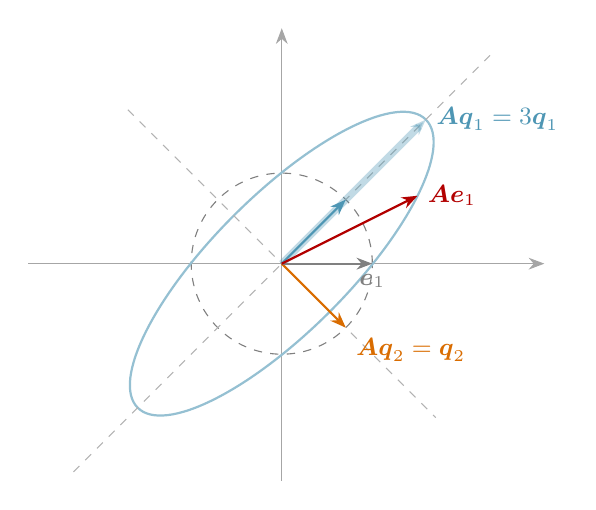
\begin{tikzpicture}[scale=1.15]
			\draw[axis] (-2.8,0) -- (2.9,0);
			\draw[axis] (0,-2.4) -- (0,2.6);
			\draw[gray,dashed] (0,0) circle (1);
			\draw[thick,figblue!60] (0,0) [rotate=45] ellipse (3*0.75 and 1*0.75);
			\draw[gray!60,dashed] (-2.3,-2.3) -- (2.3,2.3);
			\draw[gray!60,dashed] (-1.7,1.7) -- (1.7,-1.7);
			% eigen direction (1,1): stretched by 3
			\draw[vec,figblue,line width=2.6pt,opacity=0.35] (0,0) -- (1.59,1.59);
			\draw[vec,figblue] (0,0) -- (0.707,0.707);
			\node[figblue,right,font=\small] at (1.6,1.6) {$\vv A\vv q_1=3\vv q_1$};
			% eigen direction (1,-1): unchanged
			\draw[vec,figorange] (0,0) -- (0.707,-0.707) node[below right,font=\small]{$\vv A\vv q_2=\vv q_2$};
			% generic vector e1 -> (2,1)
			\draw[vec,gray] (0,0) -- (1,0) node[below,font=\small]{$\vv e_1$};
			\draw[vec,figred] (0,0) -- (1.5,0.75) node[right,font=\small]{$\vv A\vv e_1$};
		\end{tikzpicture}
		\caption{$\vv A=\begin{pmatrix}2&1\\1&2\end{pmatrix}$ 把单位圆（虚线）变成椭圆. 两个特征方向只被伸缩：$\vv q_1$ 方向放大 $3$ 倍，$\vv q_2$ 方向不变；其他向量（如 $\vv e_1$）的方向被改变. 图中长度统一缩小为 $0.75$ 倍.}
		\label{fig:eigenellipse}
	\end{figure}
	\begin{example}
		旋转矩阵 $\vv R=\begin{pmatrix}\cos\theta&-\sin\theta\\ \sin\theta&\cos\theta\end{pmatrix}$ 的特征多项式为 $\lambda^2-2\lambda\cos\theta+1$，判别式 $4\cos^2\theta-4\le0$. 当 $\theta\ne0,\pi$ 时它没有实根：$\vv R$ 作为实矩阵\textbf{没有}特征值，这与``旋转没有一维不变子空间''相符. 若在 $\mathbb{C}$ 上考虑，它有两个特征值 $\cos\theta\pm\mathrm i\sin\theta$.
	\end{example}
	
	\begin{pitfallbox}
		\begin{enumerate}
			\item 特征值依赖于数域：同一个实矩阵，在 $\mathbb{R}$ 上可能没有特征值，在 $\mathbb{C}$ 上一定有（代数基本定理）.
			\item \textbf{初等行变换会改变特征值}. 不要先把 $\vv A$ 化成阶梯形再求特征值！行变换对应左乘可逆矩阵 $\vv P$，而 $\vv{PA}$ 与 $\vv A$ 一般不相似.
			\item 特征向量不唯一：属于 $\lambda$ 的特征向量的非零倍数仍是特征向量. 一个特征值对应的是一整个特征子空间.
		\end{enumerate}
	\end{pitfallbox}
	
	\begin{theorem}\label{thm:charpoly}
		\begin{enumerate}
			\item $f_{\vv A}(\lambda)=\lambda^n-(\tr\vv A)\lambda^{n-1}+\cdots+(-1)^n\det\vv A$，其中 $\tr\vv A$ 是 $\vv A$ 的迹（第三章）.
			\item 若 $\vv A$ 在 $\mathbb{C}$ 中的 $n$ 个特征值（按重数计）为 $\lambda_1,\ldots,\lambda_n$，则
			\[\operatorname{tr}\vv A=\lambda_1+\cdots+\lambda_n,\qquad\det\vv A=\lambda_1\cdots\lambda_n.\]
			\item 相似矩阵有相同的特征多项式，从而有相同的特征值、迹与行列式.
		\end{enumerate}
	\end{theorem}
	\begin{proof}
		(1) 按定义展开 $\det(\lambda\vv I-\vv A)$. 含 $\lambda^n$ 与 $\lambda^{n-1}$ 的项只能来自主对角元之积 $(\lambda-a_{11})\cdots(\lambda-a_{nn})$——任何其他项至少缺两个对角元，次数 $\le n-2$. 这个乘积中 $\lambda^{n-1}$ 的系数为 $-\sum a_{ii}$. 令 $\lambda=0$ 得常数项 $\det(-\vv A)=(-1)^n\det\vv A$.
		
		(2) 由代数基本定理（定理~\ref{thm:fta}，或附录~\ref{app:complex}），$f_{\vv A}(\lambda)=(\lambda-\lambda_1)\cdots(\lambda-\lambda_n)$，再比较系数（Vieta 定理，同上）.
		
		(3) $\det(\lambda\vv I-\vv P^{-1}\vv{AP})=\det\big(\vv P^{-1}(\lambda\vv I-\vv A)\vv P\big)=\det(\lambda\vv I-\vv A)$.
	\end{proof}
	
	由 (3)，线性变换 $\mathscr T$ 在任一组基下的矩阵有相同的特征多项式，称之为 $\mathscr T$ 的特征多项式. 迹与行列式是最容易计算的两个\textbf{相似不变量}\index{xiang1si4 bu4bian4liang4@相似不变量}，常用来检验特征值算得对不对：例~\ref{eg:eig2112} 中 $1+3=4=\operatorname{tr}\vv A$，$1\times3=3=\det\vv A$.
	
	\subsection{两种重数}
	
	\begin{definition}
		特征值 $\lambda_0$ 作为特征多项式的根的重数，称为它的\textbf{代数重数}\index{dai4shu4 chong2shu4@代数重数}；$\dim V_{\lambda_0}$ 称为它的\textbf{几何重数}\index{ji3he2 chong2shu4@几何重数}.
	\end{definition}
	
	\begin{theorem}\label{thm:geoalg}
		几何重数不超过代数重数.
	\end{theorem}
	\begin{proof}
		设 $\dim V_{\lambda_0}=g$. $V_{\lambda_0}$ 是不变子空间，$\mathscr T$ 在其上就是数乘 $\lambda_0$. 由定理~\ref{thm:blockform}，取适当的基，$\mathscr T$ 的矩阵为 $\begin{pmatrix}\lambda_0\vv I_g&\vv A_2\\ \vv O&\vv A_3\end{pmatrix}$. 按第一列逐次展开，特征多项式为 $(\lambda-\lambda_0)^g\det(\lambda\vv I-\vv A_3)$，故 $\lambda_0$ 的代数重数至少为 $g$.
	\end{proof}
	
	\begin{example}
		$\vv J=\begin{pmatrix}1&1\\0&1\end{pmatrix}$ 的特征多项式为 $(\lambda-1)^2$，特征值 $1$ 的代数重数为 $2$. 但 $\vv J-\vv I=\begin{pmatrix}0&1\\0&0\end{pmatrix}$ 的秩为 $1$，$V_1$ 是一维的（$x$ 轴），几何重数为 $1$. 这个``剪切''变换只有一个不动的方向.
	\end{example}
	\begin{figure}[htbp]
		\centering
		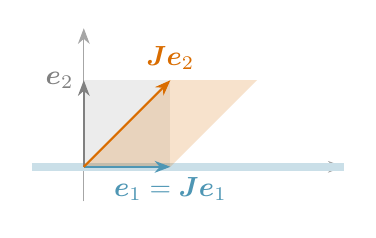
\begin{tikzpicture}[scale=1.1]
			\draw[axis] (-0.6,0) -- (3.0,0);
			\draw[axis] (0,-0.4) -- (0,1.6);
			\draw[line width=3pt,figblue!30] (-0.6,0) -- (3.0,0);
			\fill[gray,opacity=0.15] (0,0) rectangle (1,1);
			\fill[figorange,opacity=0.2] (0,0) -- (1,0) -- (2,1) -- (1,1) -- cycle;
			\draw[vec,figblue] (0,0) -- (1,0) node[below]{$\vv e_1=\vv J\vv e_1$};
			\draw[vec,gray] (0,0) -- (0,1) node[left]{$\vv e_2$};
			\draw[vec,figorange] (0,0) -- (1,1) node[above]{$\vv J\vv e_2$};
		\end{tikzpicture}
		\caption{剪切 $\vv J=\begin{pmatrix}1&1\\0&1\end{pmatrix}$ 把正方形推成平行四边形. 只有 $x$ 轴方向保持不变：它只有一个一维不变子空间，不可对角化.}
		\label{fig:shear}
	\end{figure}
	\section{相似对角化}
	
	\begin{definition}
		若方阵 $\vv A$ 与对角矩阵相似，称 $\vv A$ \textbf{可对角化}\index{ke3 dui4jiao3hua4@可对角化}. 线性变换 $\mathscr T$ 可对角化，是指存在一组基使它的矩阵为对角矩阵.
	\end{definition}
	
	\begin{theorem}\label{thm:diagbasis}
		$n$ 阶方阵 $\vv A$ 可对角化，当且仅当 $\vv A$ 有 $n$ 个线性无关的特征向量. 这时以它们为列作 $\vv P=(\vv p_1,\ldots,\vv p_n)$，有
		\[\vv P^{-1}\vv{AP}=\diag(\lambda_1,\ldots,\lambda_n),\]
		其中 $\lambda_i$ 是 $\vv p_i$ 所属的特征值.
	\end{theorem}
	\begin{proof}
		$\vv{AP}=\vv P\diag(\lambda_1,\ldots,\lambda_n)$ 逐列看就是 $\vv A\vv p_i=\lambda_i\vv p_i$. 而 $\vv P$ 可逆当且仅当它的 $n$ 列线性无关.
	\end{proof}
	
	\begin{theorem}\label{thm:distinctindep}
		属于不同特征值的特征向量线性无关. 更一般地，若 $\lambda_1,\ldots,\lambda_s$ 互不相同，则 $V_{\lambda_1}+\cdots+V_{\lambda_s}$ 是直和.
	\end{theorem}
	\begin{proof}
		先证后一句. 由命题~\ref{prop:dsum}，只需证：若 $\vv\alpha_i\in V_{\lambda_i}$ 且 $\vv\alpha_1+\cdots+\vv\alpha_s=\zero$，则每个 $\vv\alpha_i=\zero$. 对 $s$ 归纳，$s=1$ 显然. 对等式两边施以 $\mathscr T-\lambda_s\mathscr I$，由 $(\mathscr T-\lambda_s\mathscr I)\vv\alpha_i=(\lambda_i-\lambda_s)\vv\alpha_i$ 得
		\[(\lambda_1-\lambda_s)\vv\alpha_1+\cdots+(\lambda_{s-1}-\lambda_s)\vv\alpha_{s-1}=\zero.\]
		$(\lambda_i-\lambda_s)\vv\alpha_i$ 仍属于 $V_{\lambda_i}$，由归纳假设它们都为零；而 $\lambda_i\ne\lambda_s$，故 $\vv\alpha_1=\cdots=\vv\alpha_{s-1}=\zero$，从而 $\vv\alpha_s=\zero$.
		
		再证前一句. 设 $\vv p_1,\ldots,\vv p_s$ 分别是属于 $\lambda_1,\ldots,\lambda_s$ 的特征向量，且 $c_1\vv p_1+\cdots+c_s\vv p_s=\zero$. 由于 $c_i\vv p_i\in V_{\lambda_i}$，由刚证的结论，每个 $c_i\vv p_i=\zero$；而 $\vv p_i\ne\zero$，故 $c_i=0$.
	\end{proof}
	
	\begin{corollary}
		若 $n$ 阶方阵有 $n$ 个互不相同的特征值，则它可对角化.
	\end{corollary}
	
	\begin{theorem}[对角化判据]\label{thm:diagcriterion}
		设 $\lambda_1,\ldots,\lambda_s$ 是 $\vv A$ 在 $\mathbb{F}$ 中的全部互异特征值. 以下条件等价：
		\begin{enumerate}
			\item $\vv A$ 在 $\mathbb{F}$ 上可对角化；
			\item $\mathbb{F}^n=V_{\lambda_1}\oplus\cdots\oplus V_{\lambda_s}$；
			\item $\dim V_{\lambda_1}+\cdots+\dim V_{\lambda_s}=n$；
			\item 特征多项式在 $\mathbb{F}$ 上分解为一次因式之积，且每个特征值的几何重数等于代数重数.
		\end{enumerate}
	\end{theorem}
	\begin{proof}
		由定理~\ref{thm:distinctindep}，$\sum V_{\lambda_i}$ 是直和，维数为 $\sum\dim V_{\lambda_i}$（命题~\ref{prop:dsum}），故 (2)$\Leftrightarrow$(3). 把各 $V_{\lambda_i}$ 的基合起来，就得到 $\sum\dim V_{\lambda_i}$ 个线性无关的特征向量，而任何一组线性无关的特征向量都分属这些特征子空间，个数不超过这个和. 由定理~\ref{thm:diagbasis}，(1)$\Leftrightarrow$(3).
		
		(3)$\Leftrightarrow$(4)：记 $m_i$ 为 $\lambda_i$ 的代数重数，$g_i=\dim V_{\lambda_i}$. 由定理~\ref{thm:geoalg}，$\sum g_i\le\sum m_i\le n$. 第一个等号成立当且仅当每个 $g_i=m_i$，第二个等号成立当且仅当特征多项式的根全在 $\mathbb{F}$ 中.
	\end{proof}
	
	\begin{motivebox}
		条件 (2) 是本章最核心的图景：\textbf{可对角化，就是整个空间可以拆成若干个特征子空间的直和}，变换在每一块上只是简单的数乘. 这正是第二章直和理论的用武之地. 不可对角化的矩阵（如剪切 $\vv J$）缺少足够多的``只拉伸不转向''的方向.
	\end{motivebox}
	
	\subsection{矩阵的幂与差分方程}
	
	若 $\vv A=\vv P\vv D\vv P^{-1}$，$\vv D=\diag(\lambda_1,\ldots,\lambda_n)$，则
	\[\vv A^k=\vv P\vv D^k\vv P^{-1}=\vv P\diag(\lambda_1^k,\ldots,\lambda_n^k)\vv P^{-1}.\]
	中间的 $\vv P^{-1}\vv P$ 两两相消. 计算 $\vv A^{100}$ 不必做 $99$ 次矩阵乘法.
	
	\begin{example}[（Fibonacci 数列）]\label{eg:fib}
		$F_0=0$，$F_1=1$，$F_{k+1}=F_k+F_{k-1}$. 求通项.
	\end{example}
	\begin{solution}
		令 $\vv u_k=(F_{k+1},F_k)^\trans$，则 $\vv u_k=\vv A\vv u_{k-1}$，$\vv A=\begin{pmatrix}1&1\\1&0\end{pmatrix}$，所以 $\vv u_k=\vv A^k\vv u_0$. 特征多项式 $\lambda^2-\lambda-1$ 有两个不同的根
		\[\varphi=\frac{1+\sqrt5}2\approx1.618,\qquad\psi=\frac{1-\sqrt5}2\approx-0.618,\]
		对应特征向量 $(\varphi,1)^\trans$，$(\psi,1)^\trans$. 把 $\vv u_0=(1,0)^\trans$ 分解为 $\frac1{\sqrt5}\big[(\varphi,1)^\trans-(\psi,1)^\trans\big]$，每个分量在 $\vv A^k$ 作用下只乘以 $\lambda^k$，读出第二个分量得
		\[F_k=\frac{\varphi^k-\psi^k}{\sqrt5}.\]
		由于 $|\psi|<1$，$\psi^k\to0$，所以 $F_{k+1}/F_k\to\varphi$：长期行为由\textbf{绝对值最大}的特征值决定.
	\end{solution}
	
	这个例子的思路适用于一切线性递推：把状态写成向量、把递推写成矩阵，再把初始状态按特征向量分解. 每个分量各自以 $\lambda_i^k$ 的速度增长或衰减，互不干扰.
	
	\section{\hC Cayley–Hamilton 定理与最小多项式}
	
	\begin{theorem}[Cayley–Hamilton]\label{thm:cayleyhamilton}\index{cayley hamilton ding4li3@Cayley–Hamilton 定理}
		设 $f(\lambda)=\det(\lambda\vv I-\vv A)$ 是 $n$ 阶方阵 $\vv A$ 的特征多项式，则 $f(\vv A)=\vv O$.
	\end{theorem}
	\begin{proof}
		记 $\vv B(\lambda)$ 为 $\lambda\vv I-\vv A$ 的伴随矩阵. 由第五章，$(\lambda\vv I-\vv A)\vv B(\lambda)=f(\lambda)\vv I$. $\vv B(\lambda)$ 的元素是 $n-1$ 阶行列式，都是 $\lambda$ 的次数 $\le n-1$ 的多项式，所以可以按 $\lambda$ 的幂次写成
		\[\vv B(\lambda)=\vv B_0+\lambda\vv B_1+\cdots+\lambda^{n-1}\vv B_{n-1},\]
		其中 $\vv B_k$ 是数字矩阵. 设 $f(\lambda)=\lambda^n+c_{n-1}\lambda^{n-1}+\cdots+c_0$，并约定 $c_n=1$，$\vv B_{-1}=\vv B_n=\vv O$. 比较 $(\lambda\vv I-\vv A)\vv B(\lambda)=f(\lambda)\vv I$ 两边 $\lambda^k$ 的系数矩阵：
		\[\vv B_{k-1}-\vv A\vv B_k=c_k\vv I\qquad(k=0,1,\ldots,n).\]
		第 $k$ 式左乘 $\vv A^k$ 后全部相加，右边是 $\sum c_k\vv A^k=f(\vv A)$，左边是 $\sum_{k=0}^{n}\big(\vv A^k\vv B_{k-1}-\vv A^{k+1}\vv B_k\big)$，相邻项两两抵消，首末两项为 $\vv A^0\vv B_{-1}=\vv O$ 与 $\vv A^{n+1}\vv B_n=\vv O$. 故 $f(\vv A)=\vv O$.
	\end{proof}
	
	\begin{pitfallbox}
		一个流传很广的错误``证明''是：$f(\vv A)=\det(\vv A\vv I-\vv A)=\det\vv O=0$. 错在 $f(\vv A)$ 是一个\textbf{矩阵}，而右边是一个\textbf{数}：``先把 $\lambda$ 换成 $\vv A$ 再求行列式''与``先求行列式再代入 $\vv A$''是两回事.
	\end{pitfallbox}
	
	Cayley–Hamilton 定理说明：$\vv A$ 总被某个非零多项式``消灭''. 那么，能消灭 $\vv A$ 的次数最低的多项式是什么？
	
	\begin{definition}
		使 $m(\vv A)=\vv O$ 的次数最低的首一多项式 $m$ 称为 $\vv A$ 的\textbf{最小多项式}\index{zui4xiao3 duo1xiang4shi4@最小多项式}，记为 $m_{\vv A}$.
	\end{definition}
	
	\begin{theorem}\label{thm:minpoly}
		\begin{enumerate}
			\item 最小多项式唯一，并且对任意多项式 $g$，$g(\vv A)=\vv O$ 当且仅当 $m_{\vv A}\mid g$. 特别地，$m_{\vv A}$ 整除特征多项式.
			\item $m_{\vv A}$ 与特征多项式有相同的根（不计重数），即 $\vv A$ 的全部特征值.
			\item 相似矩阵有相同的最小多项式.
		\end{enumerate}
	\end{theorem}
	\begin{proof}
		(1) 用 $m=m_{\vv A}$ 除 $g$：$g=qm+r$，$\deg r<\deg m$. 代入 $\vv A$ 得 $r(\vv A)=g(\vv A)-q(\vv A)m(\vv A)=g(\vv A)$. 若 $g(\vv A)=\vv O$，则 $r(\vv A)=\vv O$，由 $m$ 次数最低，$r=0$. 唯一性：两个最小多项式互相整除且都首一，故相等.
		
		(2) 若 $\vv{Ax}=\lambda\vv x$，$\vv x\ne\zero$，则 $\vv0=m(\vv A)\vv x=m(\lambda)\vv x$，故 $m(\lambda)=0$. 反之 $m$ 整除特征多项式，$m$ 的根都是特征值.
		
		(3) $g(\vv P^{-1}\vv{AP})=\vv P^{-1}g(\vv A)\vv P$.
	\end{proof}
	
	下面这个引理是 Bézout 等式在线性代数中最漂亮的一次出场.
	
	\begin{lemma}[核分解引理]\label{lem:kerdecomp}\index{he2 fen1jie3 yin3li3@核分解引理}
		设 $f=gh$，其中 $g,h$ 互素，则对 $V$ 上的任一线性变换 $\mathscr T$，
		\[\ker f(\mathscr T)=\ker g(\mathscr T)\oplus\ker h(\mathscr T).\]
	\end{lemma}
	\begin{proof}
		由 Bézout 等式，有 $u,v$ 使 $ug+vh=1$，代入 $\mathscr T$ 得
		\[\mathscr I=u(\mathscr T)g(\mathscr T)+v(\mathscr T)h(\mathscr T).\]
		对 $\vv\alpha\in\ker f(\mathscr T)$，令 $\vv\alpha_1=v(\mathscr T)h(\mathscr T)\vv\alpha$，$\vv\alpha_2=u(\mathscr T)g(\mathscr T)\vv\alpha$，则 $\vv\alpha=\vv\alpha_1+\vv\alpha_2$，且
		\[g(\mathscr T)\vv\alpha_1=v(\mathscr T)f(\mathscr T)\vv\alpha=\zero,\qquad h(\mathscr T)\vv\alpha_2=u(\mathscr T)f(\mathscr T)\vv\alpha=\zero,\]
		即 $\vv\alpha_1\in\ker g(\mathscr T)$，$\vv\alpha_2\in\ker h(\mathscr T)$. 反过来 $\ker g(\mathscr T)$ 与 $\ker h(\mathscr T)$ 都含于 $\ker f(\mathscr T)$. 最后，若 $\vv\alpha$ 同属两者，则 $\vv\alpha=u(\mathscr T)g(\mathscr T)\vv\alpha+v(\mathscr T)h(\mathscr T)\vv\alpha=\zero$，和是直和.
	\end{proof}
	
	\begin{theorem}\label{thm:minpolydiag}
		方阵 $\vv A$ 在 $\mathbb{F}$ 上可对角化，当且仅当它的最小多项式在 $\mathbb{F}$ 上分解为\textbf{互不相同}的一次因式之积.
	\end{theorem}
	\begin{proof}
		\textbf{必要性.} 设 $\vv A=\vv P\vv D\vv P^{-1}$，$\vv D$ 的互异对角元为 $\lambda_1,\ldots,\lambda_s$. 令 $g=(x-\lambda_1)\cdots(x-\lambda_s)$，则 $g(\vv D)$ 是对角矩阵，每个对角元都含一个为零的因子，故 $g(\vv D)=\vv O$，$g(\vv A)=\vv Pg(\vv D)\vv P^{-1}=\vv O$. 于是 $m_{\vv A}\mid g$，它也是互异一次因式之积.
		
		\textbf{充分性.} 设 $m_{\vv A}=(x-\lambda_1)\cdots(x-\lambda_s)$，$\lambda_i$ 互不相同. 不同的首一一次多项式互素，$x-\lambda_1$ 与 $(x-\lambda_2)\cdots(x-\lambda_s)$ 也互素（后者在 $\lambda_1$ 处不为零）. 反复使用核分解引理（对因子个数归纳），得
		\[\mathbb{F}^n=\ker m_{\vv A}(\vv A)=\ker(\vv A-\lambda_1\vv I)\oplus\cdots\oplus\ker(\vv A-\lambda_s\vv I)=V_{\lambda_1}\oplus\cdots\oplus V_{\lambda_s}.\]
		由定理~\ref{thm:diagcriterion} 即知可对角化.
	\end{proof}
	
	\begin{example}
		\begin{enumerate}
			\item 若 $\vv A^2=\vv A$（幂等矩阵），则 $\vv A$ 被 $x(x-1)$ 消灭，最小多项式整除它，是互异一次因式之积，故 $\vv A$ 可对角化，特征值只能是 $0,1$. 几何上，$\vv A$ 是沿 $V_0=\ker\vv A$ 向 $V_1=\imm\vv A$ 的投影——第四章章末习题~\ref{ex:lmap:B8} 中的分解，在这里有了特征值的解释.
			\item 若 $\vv A^2=\vv I$（例如平面上关于一条直线的反射），同理 $\vv A$ 可对角化，特征值为 $\pm1$.
			\item 剪切 $\vv J=\begin{pmatrix}1&1\\0&1\end{pmatrix}$ 的最小多项式是 $(x-1)^2$（$\vv J-\vv I\ne\vv O$），有重因式，不可对角化.
		\end{enumerate}
	\end{example}
	
	\section{\hB 应用：马尔可夫链与 PageRank}\index{pagerank@PageRank}
	
	\begin{modelbox}{消费者的品牌转移}
		\mstep{问题} 某城市的咖啡外卖市场由三个品牌 $A,B,C$ 瓜分. 市场调查发现，每个月，原来购买 $A$ 的顾客有 $80\%$ 继续购买 $A$，$10\%$ 转向 $B$，$10\%$ 转向 $C$；$B$ 的顾客有 $70\%$ 留下，$10\%$ 转向 $A$，$20\%$ 转向 $C$；$C$ 的顾客有 $60\%$ 留下，$20\%$ 转向 $A$，$20\%$ 转向 $B$. 若现在三家各占三分之一，长期来看市场份额会怎样？
		
		\mstep{假设} 顾客下个月买哪家只取决于这个月买哪家（\textbf{无记忆性}）；转移比例不随时间变化；顾客总数不变.
		
		\mstep{模型} 设第 $k$ 个月的市场份额为 $\vv x_k\in\mathbb{R}^3$，则 $\vv x_{k+1}=\vv P\vv x_k$，其中
		\[\vv P=\begin{pmatrix}0.8&0.1&0.2\\0.1&0.7&0.2\\0.1&0.2&0.6\end{pmatrix}.\]
		第 $j$ 列是第 $j$ 个品牌的顾客下个月的去向，元素非负且\textbf{列和为 $1$}. 这样的矩阵称为\textbf{转移矩阵}\index{zhuan3yi2 ju3zhen4@转移矩阵}，这个模型称为\textbf{马尔可夫链}\index{ma3er3ke3fu1 lian4@马尔可夫链}.
		\begin{center}
			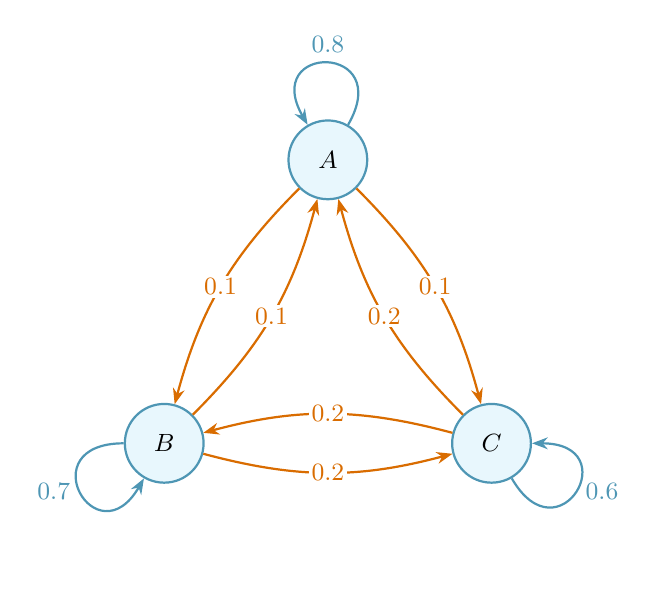
\begin{tikzpicture}[every node/.style={font=\small}]
				\node[station,minimum size=10mm] (A) at (90:2.4) {$A$};
				\node[station,minimum size=10mm] (B) at (210:2.4) {$B$};
				\node[station,minimum size=10mm] (C) at (330:2.4) {$C$};
				\draw[vec,figblue] (A) to[out=60,in=120,looseness=6] node[above]{$0.8$} (A);
				\draw[vec,figblue] (B) to[out=180,in=240,looseness=6] node[left]{$0.7$} (B);
				\draw[vec,figblue] (C) to[out=-60,in=0,looseness=6] node[right]{$0.6$} (C);
				\draw[vec,figorange] (A) to[bend right=15] node[fill=white,inner sep=1pt]{$0.1$} (B);
				\draw[vec,figorange] (B) to[bend right=15] node[fill=white,inner sep=1pt]{$0.1$} (A);
				\draw[vec,figorange] (A) to[bend left=15] node[fill=white,inner sep=1pt]{$0.1$} (C);
				\draw[vec,figorange] (C) to[bend left=15] node[fill=white,inner sep=1pt]{$0.2$} (A);
				\draw[vec,figorange] (B) to[bend right=15] node[fill=white,inner sep=1pt]{$0.2$} (C);
				\draw[vec,figorange] (C) to[bend right=15] node[fill=white,inner sep=1pt]{$0.2$} (B);
			\end{tikzpicture}
			\captionof{figure}{品牌转移的状态图. 箭头上的数是一个月内从出发品牌转到目标品牌的顾客比例；从每个品牌出发的箭头（含自环）之和为 $1$.}
			\label{fig:markov}
		\end{center}
		\mstep{求解}
		\begin{itemize}
			\item 列和为 $1$，即 $(1,1,1)\vv P=(1,1,1)$，所以 $\vv P^\trans$ 有特征值 $1$；$\vv P$ 与 $\vv P^\trans$ 有相同的特征多项式，所以 $1$ 也是 $\vv P$ 的特征值. 解 $(\vv P-\vv I)\vv x=\zero$ 并使分量和为 $1$，得
			\[\vv\pi=\tfrac1{19}(8,6,5)^\trans\approx(0.421,0.316,0.263)^\trans.\]
			它满足 $\vv P\vv\pi=\vv\pi$：若市场份额恰为 $\vv\pi$，它就永远不变. $\vv\pi$ 称为\textbf{稳态分布}\index{wen3tai4 fen1bu4@稳态分布}.
			\item 由迹与行列式，另两个特征值满足 $\lambda_2+\lambda_3=\operatorname{tr}\vv P-1=1.1$，$\lambda_2\lambda_3=\det\vv P=0.29$，解得 $\lambda_{2,3}=\frac{11\pm\sqrt5}{20}\approx0.662,\,0.438$. 三个特征值互不相同，$\vv P$ 可对角化. 把 $\vv x_0$ 按特征向量分解为 $\vv\pi+c_2\vv v_2+c_3\vv v_3$，则
			\[\vv x_k=\vv P^k\vv x_0=\vv\pi+c_2(0.662)^k\vv v_2+c_3(0.438)^k\vv v_3\ \longrightarrow\ \vv\pi.\]
			（$\vv\pi$ 前的系数为 $1$，因为 $\vv P$ 保持分量之和，而 $\vv v_2,\vv v_3$ 的分量和为零——这是习题.）
			\item 数值上，$\vv x_1\approx(0.367,0.333,0.300)^\trans$，$\vv x_6\approx(0.415,0.319,0.266)^\trans$，$\vv x_{12}\approx(0.421,0.316,0.263)^\trans$，一年后已几乎等于稳态.
		\end{itemize}
		
		\mstep{解读}
		\begin{itemize}
			\item 长期份额与\textbf{初始份额无关}，只由转移规律决定. 一次性的促销能改变 $\vv x_0$，却改变不了 $\vv\pi$；要改变长期格局，必须改变 $\vv P$——即顾客的留存率与转入率.
			\item 收敛的速度由第二大的特征值 $0.662$ 决定：偏离稳态的部分每月大约缩小到原来的三分之二.
		\end{itemize}
		
		\mstep{局限} 真实顾客有``记忆''（会员积分、使用习惯），转移比例也随价格和季节变化；市场还有新顾客进入、老顾客流失. 无记忆的假设可以通过把``状态''定义得更细来部分弥补，代价是矩阵变大.
		
	\end{modelbox}
	
	\begin{modelbox}{判例的重要性：从被引次数到 PageRank}
		\mstep{问题} 第三章的``判例引证网络''中，判决 $1$ 引用 $2,3$；$2$ 引用 $3,4$；$3$ 引用 $4$；$4$ 不引用任何判决. 被引次数为 $(0,1,2,2)$，判决 $3$ 与 $4$ 并列第一. 但直觉上，被\textbf{重要的}判决引用应该更有分量. 怎样把这个直觉变成计算？
		
		\mstep{假设} 每份判决把自己的``重要性''平均分给它所引用的判决；一份判决的重要性，等于它从引用它的判决那里分到的总和.
		
		\mstep{模型} 记重要性为 $x_1,\ldots,x_4$，判决 $j$ 引用了 $d_j$ 份判决. 假设翻译成方程：
		\[x_i=\sum_{j\ \text{引用}\ i}\frac{x_j}{d_j},\qquad\text{即}\quad \vv x=\vv S\vv x.\]
		重要性向量是矩阵 $\vv S$ 属于特征值 $1$ 的特征向量！这看似``循环定义''的问题，在线性代数里是一个干净的特征值问题.
		
		\mstep{求解}
		\begin{itemize}
			\item \textbf{困难一：悬挂结点.} 判决 $4$ 不引用任何判决，$d_4=0$，$\vv S$ 的第 $4$ 列全为零，重要性从这里``漏''掉了. 事实上，由于只能引用更早的判决，这时 $\vv S$ 是严格下三角矩阵，是\textbf{幂零}的（回忆第三章），唯一的特征值是 $0$，迭代 $\vv x\mapsto\vv{Sx}$ 会让全部重要性衰减为零. 常用的修补是：让悬挂结点把重要性平均分给所有判决. 修补后
			\[\vv S=\begin{pmatrix}0&0&0&\frac14\\ \frac12&0&0&\frac14\\ \frac12&\frac12&0&\frac14\\ 0&\frac12&1&\frac14\end{pmatrix},\]
			它成为一个转移矩阵（列和为 $1$）.
			\item \textbf{困难二：唯一性与收敛性.} 对一般的网络（有环路、有互不相连的几块），特征值 $1$ 的特征子空间可能不止一维，迭代也可能来回振荡. PageRank 的办法是引入\textbf{阻尼系数}\index{zu3ni2 xi4shu4@阻尼系数} $d$（常取 $0.85$）：
			\[\vv G=d\,\vv S+\frac{1-d}{n}\vv J,\]
			$\vv J$ 是元素全为 $1$ 的矩阵. 它的含义是一位``随机阅读者''：以概率 $d$ 沿着引用链接读下去，以概率 $1-d$ 随机翻开任意一份判决. $\vv G$ 的元素全为正，由 Perron–Frobenius 定理（陈述从略），它的特征值 $1$ 是单根，有唯一的分量和为 $1$ 的正特征向量，且迭代必收敛于它.
			\item 本例求得 $\vv x\approx(0.128,\ 0.183,\ 0.261,\ 0.428)^\trans$.
		\end{itemize}
		\begin{center}
			\begin{tikzpicture}
				\foreach \i/\x/\s in {1/0/0.128,2/2.4/0.183,3/4.8/0.261,4/7.2/0.428}{
					\node[circle,draw=figblue,thick,fill=customcolor!30,minimum size={22mm*sqrt(\s)},inner sep=0pt] (n\i) at (\x,0) {$\i$};
					\node[font=\small] at (\x,-2.3) {$\s$};
				}
				\draw[vec,figblue] (n1) -- (n2);
				\draw[vec,figblue] (n2) -- (n3);
				\draw[vec,figblue] (n3) -- (n4);
				\draw[vec,figblue] (n1) to[bend left=40] (n3);
				\draw[vec,figblue] (n2) to[bend left=45] (n4);
				\draw[->,gray,dashed] (n4) to[bend left=35] (n3);
				\draw[->,gray,dashed] (n4) to[bend left=45] (n2);
				\draw[->,gray,dashed] (n4) to[bend left=50] (n1);
				\node[font=\small,anchor=east] at (-0.6,-2.3) {分数};
			\end{tikzpicture}
			\captionof{figure}{判例引证网络的 PageRank（$d=0.85$）. 结点面积正比于分数. 判决 $3$、$4$ 被引次数相同，但 $4$ 被重要的判决 $3$ 引用，分数明显更高. 灰色虚线是对悬挂结点 $4$ 的修补：它把重要性平均分给所有判决（指向自己的那份未画出）. 与图~\ref{fig:citation} 对照.}
			\label{fig:pagerank}
		\end{center}
		\mstep{解读} 判决 $3$ 与 $4$ 被引次数相同，PageRank 却把 $4$ 排得明显更高：引用 $4$ 的判决 $3$ 本身就很重要，而引用 $3$ 的判决 $1$ 无人引用. 重要性沿着引证链条\textbf{传递}. 搜索引擎给网页排序、学术界评价论文、法律数据库给判例排序，用的都是这一思想的变体.
		
		\mstep{局限}
		\begin{itemize}
			\item 引用有态度：``本院不予采纳''式的否定性引用也会抬高被引判决的分数. 可以给引用加权甚至允许负权，但那时 Perron–Frobenius 定理不再适用.
			\item 时间偏差：越早的判决积累引用的时间越长. 实际应用中常按时间窗口归一化.
			\item 随机跳转默认``均匀地''翻开任意判决. 若让随机跳转偏向指导性案例（\textbf{个性化 PageRank}），就把法律上的效力层级编进了模型——这是建模者的价值选择，不是数学的结论.
		\end{itemize}
	\end{modelbox}
	
	\begin{historybox}{从普希金的诗到搜索引擎}
		\sidefig[0.25\linewidth]{image/markov.jpg}{马尔可夫}[fig:portraitmarkov]
		1906 年，俄国数学家马尔可夫（A.~A.~Markov）提出了``下一步只依赖当前状态''的随机过程，用以反驳``大数定律只对独立事件成立''的说法\cite{markov1906rasprostranenie}. 1913 年，他统计了普希金《叶甫盖尼·奥涅金》前两万个字母中元音与辅音的交替规律，这是马尔可夫链的第一次``实证应用''\cite{markov1913onegin,hayes2013first}. 九十年后，斯坦福大学的研究生布林（S.~Brin）与佩奇（L.~Page）在 1998 年的论文\cite{brin1998anatomy}中提出了 PageRank——一个规模达数亿的马尔可夫链的稳态分布.
	\end{historybox}
	
	\section{*Jordan 标准形（选读）}
	
	不是每个矩阵都能对角化. 那么，在相似的意义下，一个矩阵最简单能化成什么样子？
	
	\begin{definition}
		形如
		\[\vv J_k(\lambda)=\begin{pmatrix}\lambda&1&&\\&\lambda&\ddots&\\&&\ddots&1\\&&&\lambda\end{pmatrix}_{k\times k}\]
		的矩阵称为 $k$ 阶 \textbf{Jordan 块}\index{jordan kuai4@Jordan 块}（主对角线上为 $\lambda$，紧邻其上的一条斜线上为 $1$，其余为 $0$）. 由 Jordan 块组成的分块对角矩阵称为 \textbf{Jordan 矩阵}.
	\end{definition}
	
	\begin{theorem}[Jordan 标准形]\index{jordan biao1zhun3xing2 ding4li3@Jordan 标准形定理}
		每个复方阵都相似于一个 Jordan 矩阵，并且这个 Jordan 矩阵除了各 Jordan 块的排列顺序外是唯一的，称为它的 \textbf{Jordan 标准形}\index{jordan biao1zhun3xing2@Jordan 标准形}. 此外，对每个特征值 $\lambda_0$：
		\begin{itemize}
			\item 以 $\lambda_0$ 为对角元的 Jordan 块的\textbf{个数}，等于 $\lambda_0$ 的几何重数；
			\item 这些块的\textbf{阶数之和}，等于 $\lambda_0$ 的代数重数；
			\item 其中\textbf{最大的阶数}，等于 $\lambda_0$ 在最小多项式中的重数.
		\end{itemize}
	\end{theorem}
	
	完整的证明需要较多准备，留给后续课程. 可对角化恰好是``所有 Jordan 块都是一阶的''情形，与定理~\ref{thm:minpolydiag} 一致.
	
	\begin{example}
		$\vv A=\begin{pmatrix}3&1\\-1&1\end{pmatrix}$ 的特征多项式为 $(\lambda-2)^2$，而 $\vv A-2\vv I=\begin{pmatrix}1&1\\-1&-1\end{pmatrix}$ 的秩为 $1$，几何重数为 $1$，所以 Jordan 标准形为 $\vv J_2(2)$. 取 $\vv v_2=(1,0)^\trans$，$\vv v_1=(\vv A-2\vv I)\vv v_2=(1,-1)^\trans$，则 $\vv A\vv v_1=2\vv v_1$，$\vv A\vv v_2=\vv v_1+2\vv v_2$. 令 $\vv P=(\vv v_1,\vv v_2)$，得 $\vv P^{-1}\vv{AP}=\begin{pmatrix}2&1\\0&2\end{pmatrix}$.
	\end{example}
	
	由 $\vv J_2(\lambda)=\lambda\vv I+\vv N$，$\vv N^2=\vv O$，且 $\lambda\vv I$ 与 $\vv N$ 可交换，用二项式定理得
	\[\vv J_2(\lambda)^k=\lambda^k\vv I+k\lambda^{k-1}\vv N=\begin{pmatrix}\lambda^k&k\lambda^{k-1}\\0&\lambda^k\end{pmatrix}.\]
	这解释了一个中学就见过的现象：特征方程有重根 $\lambda$ 时，线性递推的通项中会出现 $k\lambda^k$ 这样的项.
	\begin{codebox}{判例的 PageRank}
		\mstep{目标} 从第三章的引证关系出发，编程算出四份判决的 PageRank，并观察阻尼系数的影响.
		
		\mstep{准备} \texttt{numpy}；第三章引证网络的邻接矩阵（$a_{ij}=1$ 表示判决 $i$ 引用判决 $j$）.
		
		\mstep{任务}
		\begin{enumerate}
			\item 写函数 \texttt{link\_matrix(A)}：按建模实验中的规则构造 $\vv S$，注意 $\vv S$ 的第 $j$ 列描述判决 $j$ 把重要性分给谁，悬挂结点平均分给所有判决. 检查每列之和都为 $1$.
			\item 写函数 \texttt{pagerank(A, d)}：构造 $\vv G$，从 $\vv x=(\frac14,\ldots,\frac14)^\trans$ 出发反复计算 $\vv x\leftarrow\vv{Gx}$，直到前后两次的分量差的绝对值之和小于 $10^{-10}$，返回结果与迭代步数.
			\item 取 $d=0.85$，与正文的结果比较.
			\item 取 $d=0.5,\ 0.85,\ 0.95,\ 1$，把四份判决的得分和迭代步数列成表（这也就完成了本章章末习题~\ref{ex:eig:B17}）.
			\item 用 \texttt{numpy.linalg.eig} 直接求 $\vv G$ 属于特征值 $1$ 的特征向量，归一化后与幂迭代的结果比较.
		\end{enumerate}
		
		\mstep{检查点} $d=0.85$ 时得分约为 $(0.128,0.183,0.261,0.428)$，约 $28$ 步收敛；$d=1$ 时恰为 $\frac1{35}(4,6,9,16)$；四种情形下判决 $4$ 都排第一.
		
		\mstep{思考}
		\begin{enumerate}
			\item 打印每种 $d$ 下 $\vv G$ 各特征值的绝对值，第二大的那个与 $d$ 有什么关系？它为什么决定了迭代的快慢？（回忆品牌转移模型中的``$0.662$''.）
			\item 若给否定性引用赋予负权重，$\vv S$ 还是转移矩阵吗？幂迭代还一定收敛吗？
		\end{enumerate}
	\end{codebox}
	\newpage
	\ExEigen
	
	% =====================================================================
	
	\chapter{内积空间}\label{ch:innerproduct}

	\paragraph*{本章地位}
	
	此前的向量空间只有加法与数乘，没有长度和角度. 本章在向量空间上引入内积，由此定义长度、夹角与正交，并建立标准正交基与 Gram–Schmidt 正交化方法. 在此基础上，本章讨论正交投影与最小二乘法，以及保持内积的正交变换与正交矩阵. 内积是第十章的谱定理与奇异值分解、第十一章的二次型所必需的工具.
	
	\chapterhours{3}{5}{6}
	
	\begin{introduction}[学习目标]
		\item 验证一个二元函数是否为内积，计算向量的长度、夹角与距离
		\item 运用 Cauchy–Schwarz 不等式
		\item 用 Gram–Schmidt 方法把线性无关组化为标准正交组
		\item 判断矩阵是否为正交矩阵，说明正交变换保持长度与内积
		\item 求向量在子空间上的正交投影，用正规方程求最小二乘解（64 学时方案起）
	\end{introduction}
	
	\paragraph*{前置知识}
	
	第二章（基与维数）；第三章（矩阵的运算与逆矩阵）；中学的向量数量积.
	
	\paragraph*{学习提示}
	\begin{itemize}
		\item 本章的概念大多可以在平面和空间中直观理解. 学习时应先在二维、三维的情形下作图，再看它们如何推广到 $n$ 维和一般的内积空间.
		\item 在标准正交基下，求坐标只需计算内积；正交投影给出子空间中与给定向量距离最近的点. 这两点是本章各项应用（包括最小二乘法）的共同基础.
		\item 正交矩阵对应于保持长度与角度的变换. 第十、十一章的正交对角化，都是在正交矩阵的范围内选取基.
	\end{itemize}
	
	\newpage
	\begin{tcolorbox}[epigraph, epigraph image*={0.3\linewidth}{image/hilbert.jpg}{大卫·希尔伯特}{fig:hilbert}]
	\begin{quote}Man muß jederzeit an Stelle von „Punkte, Geraden, Ebenen“ „Tische, Stühle, Bierseidel“ sagen können.\end{quote}
	\begin{flushright}——David Hilbert\end{flushright}
	\begin{quote}无论何时，都必须能够把``点、直线、平面''换成``桌子、椅子、啤酒杯''来说.\end{quote}
	\begin{flushright}——大卫·希尔伯特\footnotemark\end{flushright}
	\end{tcolorbox}
	\footnotetext{大卫·希尔伯特（1862—1943），德国数学家，20 世纪初最有影响的数学家之一，公理化方法的倡导者. 据布卢门塔尔（O.~Blumenthal）为《希尔伯特全集》第三卷（1935）所写的传记，这是希尔伯特 1891 年前后在柏林火车站候车时说的话，其精神后来体现在《几何基础》（1899）中：几何对象是什么无关紧要，要紧的只是公理规定的关系. 本章的``长度''``角度''也是如此——只要满足内积公理，函数之间也有夹角.}
	\section{内积与范数}\label{sec:innerproduct}
	
	在平面上，向量 $\vv a=(a_1,a_2)^\trans$ 的长度为 $\sqrt{a_1^2+a_2^2}$；由余弦定理，两个向量的夹角 $\theta$ 满足
	\[|\vv a|\,|\vv b|\cos\theta=a_1b_1+a_2b_2.\]
	右边这个``对应分量相乘再相加''的量，同时编码了长度（$\vv a$ 与自己作）与角度. 我们把它的基本性质抽出来作为定义.
	
	\begin{definition}\label{def:innerproduct}
		设 $V$ 是实向量空间. 若对任意 $\vv\alpha,\vv\beta\in V$ 有一个实数 $\langle\vv\alpha,\vv\beta\rangle$ 与之对应，且满足：对一切 $\vv\alpha,\vv\beta,\vv\gamma\in V$，$k\in\mathbb{R}$，
		\begin{enumerate}
			\item （对称性）$\langle\vv\alpha,\vv\beta\rangle=\langle\vv\beta,\vv\alpha\rangle$；
			\item （线性）$\langle\vv\alpha+\vv\beta,\vv\gamma\rangle=\langle\vv\alpha,\vv\gamma\rangle+\langle\vv\beta,\vv\gamma\rangle$，$\langle k\vv\alpha,\vv\beta\rangle=k\langle\vv\alpha,\vv\beta\rangle$；
			\item （正定性）$\langle\vv\alpha,\vv\alpha\rangle\ge0$，且等号成立当且仅当 $\vv\alpha=\zero$，
		\end{enumerate}
		则称 $\langle\cdot,\cdot\rangle$ 是 $V$ 上的一个\textbf{内积}\index{nei4ji1@内积}，配备了内积的实向量空间称为\textbf{实内积空间}\index{shi2 nei4ji1 kong1jian1@实内积空间}；有限维的实内积空间也称为\textbf{欧几里得空间}\index{ou1ji3li3de2 kong1jian1@欧几里得空间}.
	\end{definition}
	
	由对称性，内积对第二个变量也是线性的.
	
	\begin{example}
		\begin{enumerate}
			\item $\mathbb{R}^n$ 上的\textbf{标准内积}\index{biao1zhun3 nei4ji1@标准内积} $\langle\vv x,\vv y\rangle=\vv x^\trans\vv y=x_1y_1+\cdots+x_ny_n$. 本书提到 $\mathbb{R}^n$ 时，若不加说明，都配备这个内积.
			\item 加权内积 $\langle\vv x,\vv y\rangle=w_1x_1y_1+\cdots+w_nx_ny_n$（$w_i>0$）. 例如在计算价格指数时给不同商品不同的权重.
			\item $C[a,b]$ 上 $\langle f,g\rangle=\int_a^bf(x)g(x)\,\mathrm dx$. 正定性用到连续函数的性质：非负连续函数积分为零，则它恒为零.
			\item $M_{m\times n}(\mathbb{R})$ 上 $\langle\vv A,\vv B\rangle=\operatorname{tr}(\vv A^\trans\vv B)=\sum_{i,j}a_{ij}b_{ij}$，即把矩阵``拉直''成 $mn$ 维向量后的标准内积.
		\end{enumerate}
	\end{example}
	
	\begin{definition}
		称 $\|\vv\alpha\|=\sqrt{\langle\vv\alpha,\vv\alpha\rangle}$ 为 $\vv\alpha$ 的\textbf{范数}\index{fan4shu4@范数}（长度）. 长度为 $1$ 的向量称为\textbf{单位向量}\index{dan1wei4 xiang4liang4@单位向量}；对 $\vv\alpha\ne\zero$，$\vv\alpha/\|\vv\alpha\|$ 称为把 $\vv\alpha$ \textbf{单位化}. 若 $\langle\vv\alpha,\vv\beta\rangle=0$，称 $\vv\alpha$ 与 $\vv\beta$ \textbf{正交}\index{zheng4jiao1@正交}，记为 $\vv\alpha\perp\vv\beta$.
	\end{definition}
	
	\begin{theorem}[Cauchy–Schwarz 不等式]\label{thm:cauchyschwarz}\index{cauchy schwarz bu4deng3shi4@Cauchy–Schwarz 不等式}
		对任意 $\vv\alpha,\vv\beta\in V$，
		\[|\langle\vv\alpha,\vv\beta\rangle|\le\|\vv\alpha\|\,\|\vv\beta\|,\]
		等号成立当且仅当 $\vv\alpha,\vv\beta$ 线性相关.
	\end{theorem}
	\begin{proof}
		$\vv\beta=\zero$ 时显然. 设 $\vv\beta\ne\zero$，对任意实数 $t$，由正定性
		\[0\le\langle\vv\alpha-t\vv\beta,\vv\alpha-t\vv\beta\rangle=\|\vv\beta\|^2t^2-2\langle\vv\alpha,\vv\beta\rangle t+\|\vv\alpha\|^2.\]
		一个开口向上、处处非负的二次函数，判别式 $\le0$：$4\langle\vv\alpha,\vv\beta\rangle^2-4\|\vv\alpha\|^2\|\vv\beta\|^2\le0$. 等号成立当且仅当二次函数有零点 $t_0$，即 $\vv\alpha=t_0\vv\beta$.
	\end{proof}
	
	\begin{corollary}
		\begin{enumerate}
			\item （三角不等式）$\|\vv\alpha+\vv\beta\|\le\|\vv\alpha\|+\|\vv\beta\|$；
			\item （勾股定理）若 $\vv\alpha\perp\vv\beta$，则 $\|\vv\alpha+\vv\beta\|^2=\|\vv\alpha\|^2+\|\vv\beta\|^2$.
		\end{enumerate}
	\end{corollary}
	\begin{proof}
		展开 $\|\vv\alpha+\vv\beta\|^2=\|\vv\alpha\|^2+2\langle\vv\alpha,\vv\beta\rangle+\|\vv\beta\|^2$，对中间项分别用 Cauchy–Schwarz 不等式和正交条件.
	\end{proof}
	
	由 Cauchy–Schwarz 不等式，对非零向量 $\vv\alpha,\vv\beta$，$\dfrac{\langle\vv\alpha,\vv\beta\rangle}{\|\vv\alpha\|\,\|\vv\beta\|}\in[-1,1]$，于是可以\textbf{定义}它们的夹角 $\theta\in[0,\pi]$：
	\[\cos\theta=\frac{\langle\vv\alpha,\vv\beta\rangle}{\|\vv\alpha\|\,\|\vv\beta\|}.\]
	在 $\mathbb{R}^2$ 和 $\mathbb{R}^3$ 中这就是通常的夹角；在高维空间中，它是一个定义，而不等式保证了这个定义有意义.
	\begin{figure}[htbp]
		\centering
		\begin{tikzpicture}[scale=1.1]
			\coordinate (O) at (0,0);
			\coordinate (b) at (3.2,0.85);
			\coordinate (a) at (1.6,2.0);
			\coordinate (p) at ($(O)!(a)!(b)$);
			\draw[gray!60] (O) -- ($(O)!1.15!(b)$);
			\draw[vec,figblue] (O) -- (b) node[right]{$\vv\beta$};
			\draw[vec,figred] (O) -- (a) node[above]{$\vv\alpha$};
			\draw[dashed,gray] (a) -- (p);
			\draw[vec,figorange,line width=1.4pt] (O) -- (p) node[below right]{$\dfrac{\langle\vv\alpha,\vv\beta\rangle}{\langle\vv\beta,\vv\beta\rangle}\vv\beta$};
			\pic[draw,gray,angle radius=2.2mm] {right angle=a--p--O};
			\pic[draw,figred,"$\theta$",angle radius=7mm,angle eccentricity=1.35] {angle=b--O--a};
		\end{tikzpicture}
		\caption{夹角与投影. $\vv\alpha$ 在 $\vv\beta$ 方向上的``影子''长 $\|\vv\alpha\|\cos\theta$.}
		\label{fig:projline}
	\end{figure}
	\begin{linkbox}{法条检索（续）：余弦相似度}
		第三章用 $\vv A^\trans\vv q$ 给法条打分，分数是查询与法条的``共同词数''. 它有一个明显的缺陷：\textbf{长条文天然得分高}. 设只看三个关键词（违约、赔偿、离婚），查询为 $\vv q=(1,1,0)^\trans$. 法条甲是一条很长的综合性条文，词频为 $(5,1,4)^\trans$；法条乙是一条短小的违约责任条款，词频为 $(1,1,0)^\trans$. 内积打分：甲得 $6$ 分，乙得 $2$ 分. 但乙显然更切题.
		
		改用夹角的余弦打分：
		\[\cos\theta_{\text{甲}}=\frac{6}{\sqrt2\cdot\sqrt{42}}\approx0.65,\qquad \cos\theta_{\text{乙}}=\frac{2}{\sqrt2\cdot\sqrt2}=1.\]
		余弦只看\textbf{方向}、不看长度：它比较的是``用词的比例''，而不是``用词的多少''. 这就是信息检索中的\textbf{余弦相似度}\index{yu2xian2 xiang1si4du4@余弦相似度}. 顺带一提，统计学中两个变量的\textbf{相关系数}\index{xiang1guan1 xi4shu4@相关系数}，正是把两个数据向量各自减去均值之后的夹角余弦.
		\begin{center}
			\begin{tikzpicture}[iso,scale=1.25]
				\coordinate (O) at (0,0,0);
				\draw[axis] (O) -- (1.8,0,0) node[below left]{赔偿};
				\draw[axis] (O) -- (0,2.6,0) node[right]{违约};
				\draw[axis] (O) -- (0,0,2.0) node[above]{离婚};
				\coordinate (q) at (0.9,0.9,0);
				\coordinate (yi) at (0.45,0.45,0);
				\coordinate (jia) at (0.4,2.0,1.6);
				\draw[vec,figblue,line width=2.5pt,opacity=0.35] (O) -- (q);
				\draw[vec,figorange] (O) -- (yi);
				\node[figblue,below right,font=\small] at (q) {查询 $\vv q$};
				\node[figorange,above left,font=\small] at (yi) {乙};
				\draw[vec,figred] (O) -- (jia) node[above right,font=\small]{甲（长条文）};
				\draw[dashed,gray] (jia) -- (0.4,2.0,0) -- (O);
				\pic[draw,figred,"$\theta_{\text{甲}}$",angle radius=9mm,angle eccentricity=1.4] {angle=q--O--jia};
			\end{tikzpicture}
			\captionof{figure}{余弦相似度只看方向. 短条文乙与查询方向完全一致（$\cos\theta=1$）；长条文甲虽然``共同词数''更多，方向却偏离了查询. 图中向量长度按比例缩小.}
			\label{fig:cosine}
		\end{center}
	\end{linkbox}
	
	\begin{remark}
		在复向量空间上，内积的对称性要改为 $\langle\vv\alpha,\vv\beta\rangle=\overline{\langle\vv\beta,\vv\alpha\rangle}$（例如 $\mathbb{C}^n$ 上 $\langle\vv x,\vv y\rangle=\sum x_i\bar y_i$），否则 $\langle\vv\alpha,\vv\alpha\rangle$ 不一定是非负实数. 本书只在第十章的一个证明中用到复数的取共轭，其余都在实数范围内讨论.
	\end{remark}
	
	\section{正交基与 Gram–Schmidt 正交化}\label{sec:gramschmidt}
	
	\begin{definition}
		两两正交的非零向量组称为\textbf{正交向量组}；若其中每个向量都是单位向量，称为\textbf{标准正交向量组}. $n$ 维内积空间中由 $n$ 个向量构成的标准正交向量组称为\textbf{标准正交基}\index{biao1zhun3 zheng4jiao1 ji1@标准正交基}.
	\end{definition}
	
	\begin{proposition}\label{prop:orthindep}
		正交向量组线性无关. 若 $\vv e_1,\ldots,\vv e_n$ 是标准正交基，则对任意 $\vv\alpha\in V$，
		\[\vv\alpha=\sum_{i=1}^n\langle\vv\alpha,\vv e_i\rangle\vv e_i,\qquad \|\vv\alpha\|^2=\sum_{i=1}^n\langle\vv\alpha,\vv e_i\rangle^2.\]
	\end{proposition}
	\begin{proof}
		若 $\sum k_i\vv\alpha_i=\zero$，与 $\vv\alpha_j$ 作内积，正交性使其余项消失，得 $k_j\|\vv\alpha_j\|^2=0$，故 $k_j=0$. 对标准正交基，设 $\vv\alpha=\sum x_i\vv e_i$，与 $\vv e_j$ 作内积得 $x_j=\langle\vv\alpha,\vv e_j\rangle$；第二式由勾股定理.
	\end{proof}
	
	\begin{motivebox}
		在一般的基下求坐标，要解一个线性方程组；在标准正交基下求坐标，只需要作 $n$ 次内积，各个坐标互不牵连. 这就是标准正交基受欢迎的原因：\textbf{它让``分解''变得免费}.
	\end{motivebox}
	\begin{figure}[htbp]
		\centering
		\begin{tikzpicture}[scale=1.15]
			\coordinate (O) at (0,0);
			\coordinate (a1) at (3,0.5);
			\coordinate (a2) at (1.2,2.0);
			\coordinate (p) at ($(O)!(a2)!(a1)$);
			\draw[vec,figblue] (O) -- (a1) node[right]{$\vv\alpha_1=\vv\beta_1$};
			\draw[vec,gray] (O) -- (a2) node[above]{$\vv\alpha_2$};
			\draw[vec,figorange,dashed] (O) -- (p);
			\node[below=6pt,figorange,font=\small] at (p) {$\vv\alpha_2$ 在 $\vv\beta_1$ 上的影子};
			\draw[dashed,gray] (p) -- (a2);
			\draw[vec,figred,thick] (O) -- ($(a2)-(p)$) node[left]{$\vv\beta_2=\vv\alpha_2-$影子};
			\pic[draw,gray,angle radius=2.2mm] {right angle=a1--O--a2};
		\end{tikzpicture}
		\caption{Gram–Schmidt 正交化的一步：从 $\vv\alpha_2$ 中减去它在 $\vv\beta_1$ 方向上的影子，剩下的 $\vv\beta_2$ 与 $\vv\beta_1$ 垂直.}
		\label{fig:gramschmidt}
	\end{figure}
	\begin{theorem}[Gram–Schmidt 正交化]\label{thm:gramschmidt}\index{gram schmidt zheng4jiao1hua4@Gram–Schmidt 正交化}
		设 $\vv\alpha_1,\ldots,\vv\alpha_m$ 线性无关. 令
		\[\vv\beta_1=\vv\alpha_1,\qquad \vv\beta_k=\vv\alpha_k-\sum_{i=1}^{k-1}\frac{\langle\vv\alpha_k,\vv\beta_i\rangle}{\langle\vv\beta_i,\vv\beta_i\rangle}\vv\beta_i\quad(k=2,\ldots,m),\]
		再令 $\vv e_k=\vv\beta_k/\|\vv\beta_k\|$. 则 $\vv e_1,\ldots,\vv e_m$ 是标准正交向量组，并且对每个 $k$，
		\[\spn(\vv e_1,\ldots,\vv e_k)=\spn(\vv\alpha_1,\ldots,\vv\alpha_k).\]
		特别地，有限维内积空间都有标准正交基，且任一标准正交向量组都可扩充为标准正交基.
	\end{theorem}
	\begin{proof}
		对 $k$ 归纳. 设 $\vv\beta_1,\ldots,\vv\beta_{k-1}$ 两两正交、非零，且张成 $\spn(\vv\alpha_1,\ldots,\vv\alpha_{k-1})$. 对 $j<k$，
		\[\langle\vv\beta_k,\vv\beta_j\rangle=\langle\vv\alpha_k,\vv\beta_j\rangle-\frac{\langle\vv\alpha_k,\vv\beta_j\rangle}{\langle\vv\beta_j,\vv\beta_j\rangle}\langle\vv\beta_j,\vv\beta_j\rangle=0,\]
		因为和式中其余各项与 $\vv\beta_j$ 正交. $\vv\beta_k\ne\zero$：否则 $\vv\alpha_k$ 属于 $\spn(\vv\beta_1,\ldots,\vv\beta_{k-1})=\spn(\vv\alpha_1,\ldots,\vv\alpha_{k-1})$，与线性无关矛盾. 张成关系由 $\vv\beta_k$ 与 $\vv\alpha_k$ 相差前面向量的线性组合即得.
		
		最后一句：取任一基作正交化；若已有标准正交组，先用基扩张定理扩充为基，再对整组作正交化——前面已经标准正交的向量在过程中保持不变.
	\end{proof}
	
	几何上，$\vv\beta_k$ 是从 $\vv\alpha_k$ 中\textbf{减去它在前 $k-1$ 个向量方向上的影子}，剩下的就是``新的、垂直的''那一部分.
	
	\begin{example}
		对 $\vv\alpha_1=(1,1,0)^\trans$，$\vv\alpha_2=(1,0,1)^\trans$，$\vv\alpha_3=(0,1,1)^\trans$ 作正交化.
	\end{example}
	\begin{solution}
		$\vv e_1=\frac1{\sqrt2}(1,1,0)^\trans$.
		$\vv\beta_2=\vv\alpha_2-\frac12\vv\alpha_1=(\frac12,-\frac12,1)^\trans$，$\vv e_2=\frac1{\sqrt6}(1,-1,2)^\trans$.
		$\vv\alpha_3$ 在 $\vv e_1,\vv e_2$ 上的投影分别为 $\frac12(1,1,0)^\trans$ 与 $\frac16(1,-1,2)^\trans$，故
		\[\vv\beta_3=(0,1,1)^\trans-\tfrac12(1,1,0)^\trans-\tfrac16(1,-1,2)^\trans=\tfrac23(-1,1,1)^\trans,\qquad\vv e_3=\tfrac1{\sqrt3}(-1,1,1)^\trans.\]
		可以验证三者两两正交.
	\end{solution}
	
	\begin{corollary}[QR 分解]\index{qr fen1jie3@QR 分解}
		列满秩的 $m\times n$ 实矩阵 $\vv A$ 可以写成 $\vv A=\vv{QR}$，其中 $\vv Q$ 是 $m\times n$ 矩阵、列向量标准正交（即 $\vv Q^\trans\vv Q=\vv I_n$），$\vv R$ 是对角元为正的 $n$ 阶上三角矩阵.
	\end{corollary}
	\begin{proof}
		对 $\vv A$ 的列作 Gram–Schmidt. 由定理~\ref{thm:gramschmidt}，$\vv\alpha_k$ 是 $\vv e_1,\ldots,\vv e_k$ 的线性组合，$\vv e_k$ 的系数为 $\|\vv\beta_k\|>0$. 把系数排成矩阵即得.
	\end{proof}
	
	\section{正交投影与最小二乘}\label{sec:projection}
	
	\subsection{正交投影与最佳逼近}
	
	设 $W$ 是内积空间 $V$ 的有限维子空间，$\vv\alpha\in V$. 中学告诉我们，点到平面的最短距离是垂线段. 这一事实在任意内积空间中依然成立.
	
	\begin{definition}
		若 $\vv p\in W$ 且 $\vv\alpha-\vv p$ 与 $W$ 中每个向量都正交，称 $\vv p$ 为 $\vv\alpha$ 在 $W$ 上的\textbf{正交投影}\index{zheng4jiao1 tou2ying3@正交投影}，记为 $\vv\alpha_W$.
	\end{definition}
	
	由内积的线性，``与 $W$ 中每个向量正交''只需对 $W$ 的一组生成元检验.
	
	\begin{theorem}\label{thm:projformula}
		正交投影存在且唯一. 若 $\vv e_1,\ldots,\vv e_k$ 是 $W$ 的标准正交基，则
		\[\vv\alpha_W=\sum_{i=1}^k\langle\vv\alpha,\vv e_i\rangle\vv e_i.\]
	\end{theorem}
	\begin{proof}
		记右边为 $\vv p\in W$. 对每个 $j$，$\langle\vv\alpha-\vv p,\vv e_j\rangle=\langle\vv\alpha,\vv e_j\rangle-\langle\vv\alpha,\vv e_j\rangle=0$，所以 $\vv p$ 是正交投影. 若 $\vv p'$ 也是，则 $\vv p-\vv p'=(\vv\alpha-\vv p')-(\vv\alpha-\vv p)$ 既属于 $W$ 又与 $W$ 正交，与自己的内积为零，只能是零向量.
	\end{proof}
	
	\begin{theorem}[最佳逼近]\label{thm:bestapprox}\index{zui4jia1 bi1jin4 ding4li3@最佳逼近定理}
		对一切 $\vv\beta\in W$，$\|\vv\alpha-\vv\alpha_W\|\le\|\vv\alpha-\vv\beta\|$，等号成立当且仅当 $\vv\beta=\vv\alpha_W$.
	\end{theorem}
	\begin{proof}
		$\vv\alpha-\vv\beta=(\vv\alpha-\vv\alpha_W)+(\vv\alpha_W-\vv\beta)$，前者与 $W$ 正交，后者属于 $W$，二者正交. 由勾股定理，
		$\|\vv\alpha-\vv\beta\|^2=\|\vv\alpha-\vv\alpha_W\|^2+\|\vv\alpha_W-\vv\beta\|^2\ge\|\vv\alpha-\vv\alpha_W\|^2$.
	\end{proof}
	\begin{figure}[htbp]
		\centering
		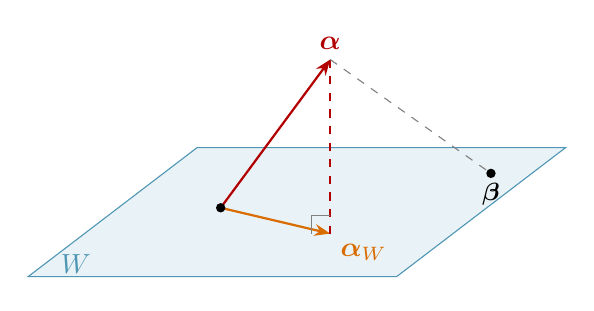
\begin{tikzpicture}[iso,scale=1.3]
			\fill[figblue,opacity=0.12] (-1.4,-1.0,0) -- (1.6,-1.0,0) -- (1.6,2.6,0) -- (-1.4,2.6,0) -- cycle;
			\draw[figblue] (-1.4,-1.0,0) -- (1.6,-1.0,0) -- (1.6,2.6,0) -- (-1.4,2.6,0) -- cycle;
			\node[figblue] at (1.3,-0.7,0) {$W$};
			\coordinate (O) at (0,0,0);
			\coordinate (a) at (0.6,1.4,1.7);
			\coordinate (p) at (0.6,1.4,0);
			\coordinate (q) at (-0.8,2.2,0);
			\draw[vec,figred] (O) -- (a) node[above]{$\vv\alpha$};
			\draw[vec,figorange] (O) -- (p) node[below right]{$\vv\alpha_W$};
			\draw[thick,dashed,figred] (a) -- (p);
			\draw[dashed,gray] (a) -- (q);
			\node[dot] at (q) {};
			\node[below,font=\small] at (q) {$\vv\beta$};
			\draw[gray] ($(p)+(0,0,0.18)$) -- ($(p)+(0,-0.18,0.18)$) -- ($(p)+(0,-0.18,0)$);
			\node[dot] at (O) {};
		\end{tikzpicture}
		\caption{在子空间 $W$ 中离 $\vv\alpha$ 最近的点，是从 $\vv\alpha$ 向 $W$ 所作垂线的垂足 $\vv\alpha_W$. $W$ 中任何别的点 $\vv\beta$ 都更远.}
		\label{fig:bestapprox}
	\end{figure}
	``在子空间里找离 $\vv\alpha$ 最近的点''，答案是``从 $\vv\alpha$ 向子空间作垂线''. 这是中学``点到平面的距离''在任意维数中的推广，也是最小二乘法的几何本质.
	
	\subsection{最小二乘}
	
	回到第六章：方程组 $\vv{Ax}=\vv y$ 无解，即 $\vv y$ 不在 $\vv A$ 的列空间 $\imm\vv A$ 中. 退而求其次，我们找使\textbf{残差}\index{can2cha1@残差} $\vv y-\vv{Ax}$ 最短的 $\vv x$：
	\[\text{求}\ \hat{\vv x}\ \text{使}\ \|\vv y-\vv A\hat{\vv x}\|\ \text{最小}.\]
	称 $\hat{\vv x}$ 为\textbf{最小二乘解}\index{zui4xiao3 er4cheng2 jie3@最小二乘解}——``二乘''指平方，$\|\vv y-\vv{Ax}\|^2$ 是各残差的平方和.
	
	\begin{theorem}[正规方程]\label{thm:normaleq}\index{zheng4gui1 fang1cheng2@正规方程}
		$\hat{\vv x}$ 是 $\vv{Ax}=\vv y$ 的最小二乘解，当且仅当
		\[\vv A^\trans\vv A\hat{\vv x}=\vv A^\trans\vv y.\]
		这个方程组总是有解的；当 $\vv A$ 列满秩时，$\vv A^\trans\vv A$ 可逆，最小二乘解唯一：$\hat{\vv x}=(\vv A^\trans\vv A)^{-1}\vv A^\trans\vv y$.
	\end{theorem}
	\begin{proof}
		$\vv A\vv x$ 取遍列空间 $W=\imm\vv A$. 由最佳逼近定理，$\|\vv y-\vv A\hat{\vv x}\|$ 最小当且仅当 $\vv A\hat{\vv x}=\vv y_W$，即 $\vv y-\vv A\hat{\vv x}$ 与 $\vv A$ 的每一列正交，写成矩阵就是 $\vv A^\trans(\vv y-\vv A\hat{\vv x})=\zero$. 由于 $\vv y_W$ 存在且属于列空间，必有 $\hat{\vv x}$ 使 $\vv A\hat{\vv x}=\vv y_W$，所以正规方程总有解.
		
		若 $\vv A$ 列满秩，设 $\vv A^\trans\vv{Ax}=\zero$，则 $\|\vv{Ax}\|^2=\vv x^\trans\vv A^\trans\vv{Ax}=0$，$\vv{Ax}=\zero$，由列满秩 $\vv x=\zero$. 故 $n$ 阶方阵 $\vv A^\trans\vv A$ 可逆.
	\end{proof}
	
	\begin{motivebox}
		正规方程不需要背：它就是``\textbf{残差与每一列垂直}''这句话的矩阵写法. 记住图像——$\vv y$ 向列空间作垂线，垂足是 $\vv A\hat{\vv x}$——公式就能随时写出来.
	\end{motivebox}
	\begin{figure}[htbp]
		\centering
		\begin{tikzpicture}[iso,scale=1.3]
			\fill[figblue,opacity=0.12] (-1.2,-1.0,0) -- (1.8,-1.0,0) -- (1.8,2.8,0) -- (-1.2,2.8,0) -- cycle;
			\draw[figblue] (-1.2,-1.0,0) -- (1.8,-1.0,0) -- (1.8,2.8,0) -- (-1.2,2.8,0) -- cycle;
			\node[figblue,font=\small,anchor=north west] at (1.8,-1.0,0) {$\imm\vv A$（列空间）};
			\coordinate (O) at (0,0,0);
			\draw[vec,figblue] (O) -- (1.3,0.3,0) node[below left]{$\vv a_1$};
			\draw[vec,figblue] (O) -- (-0.6,1.0,0) node[above]{$\vv a_2$};
			\coordinate (y) at (0.6,2.2,1.5);
			\coordinate (yh) at (0.6,2.2,0);
			\draw[vec,figred] (O) -- (y) node[above]{$\vv y$};
			\draw[vec,figorange] (O) -- (yh) node[below]{$\vv A\hat{\vv x}$};
			\draw[vec,figred,dashed,thick] (yh) -- (y) node[pos=0.5,right,font=\small]{$\vv e=\vv y-\vv A\hat{\vv x}$};
			\draw[gray] ($(yh)+(0,0,0.18)$) -- ($(yh)+(0,0.18,0.18)$) -- ($(yh)+(0,0.18,0)$);
		\end{tikzpicture}
		\caption{最小二乘的几何. $\vv y$ 不在列空间中，方程组无解；最小二乘解使 $\vv A\hat{\vv x}$ 是 $\vv y$ 在列空间上的投影，残差 $\vv e$ 与 $\vv A$ 的每一列垂直.}
		\label{fig:lsqgeom}
	\end{figure}
	\begin{modelbox}{广告与销售：最佳直线（接第六章）}
		\mstep{问题} 四个季度的广告投入 $x$（万元）与销售额 $y$（十万元）为 $(1,2)$，$(2,3)$，$(3,5)$，$(4,6)$. 求最佳直线 $y=a+bx$.
		
		\mstep{模型} 求 $\vv A\binom ab=\vv y$ 的最小二乘解，$\vv A$ 的两列分别是常数列 $(1,1,1,1)^\trans$ 与 $x$ 列 $(1,2,3,4)^\trans$.
		
		\mstep{求解} $\vv A^\trans\vv A=\begin{pmatrix}4&10\\10&30\end{pmatrix}$，$\vv A^\trans\vv y=\begin{pmatrix}16\\47\end{pmatrix}$. 正规方程 $4a+10b=16$，$10a+30b=47$ 解得
		\[a=0.5,\qquad b=1.4,\qquad y=0.5+1.4x.\]
		拟合值为 $(1.9,3.3,4.7,6.1)^\trans$，残差为 $\vv e=(0.1,-0.3,0.3,-0.1)^\trans$，残差平方和为 $0.2$.
		
		\mstep{解读}
		\begin{itemize}
			\item 斜率 $b=1.4$：广告投入每增加 $1$ 万元，销售额平均增加约 $14$ 万元.
			\item 数据围绕均值 $\bar y=4$ 的总波动为 $\sum(y_i-\bar y)^2=10$，其中残差只占 $0.2$. 统计软件报告的\textbf{决定系数}\index{jue2ding4 xi4shu4@决定系数} $R^2=1-0.2/10=0.98$. 几何上，$R^2$ 是``去均值后的 $\vv y$''与``去均值后的拟合值''夹角余弦的平方.
			\item 残差满足 $\sum e_i=0$ 与 $\sum x_ie_i=0$——它们正是正规方程本身. 这一点在第 \ref{sec:orthcomp} 节还会从``四个基本子空间''的角度再看一次.
		\end{itemize}
		
		\mstep{局限} 四个数据点太少，$R^2$ 再高也不足以支持因果结论：广告多的季度可能恰好是旺季. 第二个变量（季节）被遗漏时，斜率会把季节的作用也算在广告头上. 把季节作为第三列加入 $\vv A$，是多元回归的做法；而这样做只是让列空间多了一维，几何图像完全不变.
	\end{modelbox}
	
	\begin{historybox}{谷神星与最小二乘}
		\sidefig[0.2\linewidth]{image/ceres.jpg}{谷神星}[fig:ceres]
		1801 年元旦，意大利天文学家皮亚齐发现了一颗新的``行星''——谷神星，但只观测了四十来天它就隐没在太阳的光辉中. 当年秋天，24 岁的高斯根据这少量的观测数据算出了它的轨道，年底天文学家们果然在他预言的位置附近重新找到了它. 高斯后来说，他早在 1795 年就开始使用最小二乘法\cite{gauss1809theoria}. 而第一个公开发表这一方法的是法国数学家勒让德（1805）\cite{legendre1805nouvelles}. 两人之间由此产生了一场著名的优先权之争\cite{stigler1981gauss}.
	\end{historybox}
	
	\section{正交矩阵与正交变换}\label{sec:orthogonal}
	
	\begin{definition}
		实内积空间 $V$ 上的线性变换 $\mathscr T$ 若保持内积，即对一切 $\vv\alpha,\vv\beta\in V$，
		\[\langle\mathscr T\vv\alpha,\mathscr T\vv\beta\rangle=\langle\vv\alpha,\vv\beta\rangle,\]
		则称 $\mathscr T$ 为\textbf{正交变换}\index{zheng4jiao1 bian4huan4@正交变换}. 满足 $\vv Q^\trans\vv Q=\vv I$ 的 $n$ 阶实方阵称为\textbf{正交矩阵}\index{zheng4jiao1 ju3zhen4@正交矩阵}.
	\end{definition}
	
	\begin{theorem}\label{thm:orthequiv}
		设 $V$ 是 $n$ 维实内积空间，$\mathscr T$ 是线性变换. 以下条件等价：
		\begin{enumerate}
			\item $\mathscr T$ 是正交变换；
			\item $\mathscr T$ 保持长度：$\|\mathscr T\vv\alpha\|=\|\vv\alpha\|$；
			\item $\mathscr T$ 把某一组（从而每一组）标准正交基变为标准正交基；
			\item $\mathscr T$ 在某一组（从而每一组）标准正交基下的矩阵是正交矩阵.
		\end{enumerate}
	\end{theorem}
	\begin{proof}
		(1)$\Rightarrow$(2) 取 $\vv\beta=\vv\alpha$. (2)$\Rightarrow$(1)：由 $\|\vv\alpha+\vv\beta\|^2=\|\vv\alpha\|^2+2\langle\vv\alpha,\vv\beta\rangle+\|\vv\beta\|^2$，内积可以用长度表示：
		\[\langle\vv\alpha,\vv\beta\rangle=\tfrac12\big(\|\vv\alpha+\vv\beta\|^2-\|\vv\alpha\|^2-\|\vv\beta\|^2\big).\]
		保持长度就保持右边，从而保持内积.
		
		(1)$\Rightarrow$(3) 显然. (3)$\Rightarrow$(1)：设 $\vv e_i$ 与 $\mathscr T\vv e_i$ 都是标准正交基，由命题~\ref{prop:orthindep}，$\vv\alpha=\sum x_i\vv e_i$ 与 $\vv\beta=\sum y_i\vv e_i$ 的内积是 $\sum x_iy_i$，而 $\mathscr T\vv\alpha=\sum x_i\mathscr T\vv e_i$ 与 $\mathscr T\vv\beta$ 的内积也是 $\sum x_iy_i$.
		
		(3)$\Leftrightarrow$(4)：矩阵 $\vv Q$ 的第 $j$ 列是 $\mathscr T\vv e_j$ 在标准正交基下的坐标，坐标的标准内积就是向量的内积. $\vv Q^\trans\vv Q$ 的 $(i,j)$ 元是第 $i$ 列与第 $j$ 列的内积，所以 $\vv Q^\trans\vv Q=\vv I$ 恰好说明各列（即 $\mathscr T\vv e_j$）标准正交.
	\end{proof}
	
	\begin{proposition}\label{prop:orthmatrix}
		设 $\vv Q,\vv Q_1,\vv Q_2$ 是 $n$ 阶正交矩阵，则
		\begin{enumerate}
			\item $\vv Q^{-1}=\vv Q^\trans$，因而 $\vv Q\vv Q^\trans=\vv I$：$\vv Q$ 的各行也标准正交；
			\item $\det\vv Q=\pm1$；
			\item $\vv Q^\trans$，$\vv Q_1\vv Q_2$ 都是正交矩阵；
			\item $\vv Q$ 的实特征值只能是 $\pm1$.
		\end{enumerate}
	\end{proposition}
	\begin{proof}
		(1) 由推论~\ref{cor:onesided}. (2) $(\det\vv Q)^2=\det(\vv Q^\trans\vv Q)=1$. (3) 直接验证. (4) 若 $\vv{Qx}=\lambda\vv x$，$\vv x\ne\zero$，则 $\|\vv x\|=\|\vv{Qx}\|=|\lambda|\,\|\vv x\|$.
	\end{proof}
	
	\begin{pitfallbox}
		``各列两两正交''的矩阵\textbf{不一定}是正交矩阵：各列还必须是单位向量. 例如 $\begin{pmatrix}2&0\\0&1\end{pmatrix}$ 的两列正交，但它把 $\vv e_1$ 拉长了一倍. 名字有点误导——``标准正交矩阵''也许是更准确的叫法.
	\end{pitfallbox}
	
	\begin{theorem}[平面上的正交变换]\label{thm:orth2d}
		二阶正交矩阵只有两类：
		\[\vv R(\theta)=\begin{pmatrix}\cos\theta&-\sin\theta\\ \sin\theta&\cos\theta\end{pmatrix}\quad(\det=1),\qquad
		\vv F(\theta)=\begin{pmatrix}\cos\theta&\sin\theta\\ \sin\theta&-\cos\theta\end{pmatrix}\quad(\det=-1).\]
		前者是绕原点旋转角 $\theta$；后者是关于一条过原点、倾角为 $\theta/2$ 的直线的反射，它有特征值 $1$ 与 $-1$.
	\end{theorem}
	\begin{proof}
		第一列是单位向量，可写成 $(\cos\theta,\sin\theta)^\trans$. 第二列是与它正交的单位向量，只能是 $\pm(-\sin\theta,\cos\theta)^\trans$. $\vv F(\theta)$ 是对称矩阵，特征多项式为 $\lambda^2-1$，特征值 $\pm1$；属于 $1$ 的特征向量 $(\cos\frac\theta2,\sin\frac\theta2)^\trans$ 方向不动，属于 $-1$ 的特征向量（与之垂直）被翻转——这正是反射.
	\end{proof}
	
	由 $\vv R(\alpha)\vv R(\beta)=\vv R(\alpha+\beta)$（两次旋转的复合），比较矩阵元素就得到两角和的正弦、余弦公式（第四章章末习题~\ref{ex:lmap:A20}）.
	
	\begin{example}[（Householder 反射）]
		设 $\vv u\in\mathbb{R}^n$ 是单位向量，令 $\vv H=\vv I-2\vv u\vv u^\trans$. 则 $\vv H^\trans=\vv H$，$\vv H^\trans\vv H=\vv I-4\vv u\vv u^\trans+4\vv u(\vv u^\trans\vv u)\vv u^\trans=\vv I$，$\vv H$ 是正交矩阵. 它把 $\vv u$ 变为 $-\vv u$，而保持与 $\vv u$ 正交的每个向量不动：$\vv H$ 是关于``与 $\vv u$ 垂直的超平面''的镜面反射，称为 \textbf{Householder 反射}\index{householder fan3she4@Householder 反射}. 数值计算中，QR 分解通常不是用 Gram–Schmidt，而是用一串 Householder 反射完成的，因为后者的舍入误差小得多.
	\end{example}
	\begin{figure}[htbp]
		\centering
		\begin{tikzpicture}[scale=1.3,rotate=15]
			\fill[figblue,opacity=0.08] (0,-1.5) rectangle (2.2,1.6);
			\draw[thick,figblue] (0,-1.5) -- (0,1.6) node[above,font=\small]{超平面 $\vv u^\perp$};
			\draw[vec,figorange] (0,0) -- (0.8,0) node[below]{$\vv u$};
			\coordinate (x) at (1.6,1.0);
			\coordinate (hx) at (-1.6,1.0);
			\draw[vec,figred] (0,0) -- (x) node[right]{$\vv x$};
			\draw[vec,figred!60] (0,0) -- (hx) node[left]{$\vv H\vv x$};
			\draw[dashed,gray] (x) -- (hx);
			\draw[gray] (0,1.0) ++(0.13,0) -- ++(0,0.13) -- ++(-0.13,0);
		\end{tikzpicture}
		\caption{Householder 矩阵 $\vv H=\vv I-2\vv u\vv u^\trans$ 是关于超平面 $\vv u^\perp$ 的镜面反射：与 $\vv u$ 垂直的分量不变，沿 $\vv u$ 的分量反号.}
		\label{fig:householder}
	\end{figure}
	正交矩阵还出现在换基中：两组标准正交基之间的过渡矩阵是正交矩阵（它的列是新基在旧基下的坐标）. 于是，在标准正交基之间换基时，相似变换 $\vv P^{-1}\vv{AP}$ 就成了 $\vv P^\trans\vv{AP}$，称为\textbf{正交相似}\index{zheng4jiao1 xiang1si4@正交相似}. 第十章的主角正是它.
	
	\section{*正交补与正交分解（选读）}\label{sec:orthcomp}
	
	本节假设已读第~\ref{sec:innerproduct}—\ref{sec:orthogonal}~节：$V$ 是 $n$ 维实内积空间，内积记为 $\langle\cdot,\cdot\rangle$，$\|\vv\alpha\|=\sqrt{\langle\vv\alpha,\vv\alpha\rangle}$，且任一子空间都有标准正交基（Gram–Schmidt）. 本节的最后一部分还要用到第七章的定理~\ref{thm:realfactor} 与第八章的 Cayley–Hamilton 定理.
	
	\begin{motivebox}
		第~\ref{sec:directsum}~节告诉我们，子空间的补空间存在但不唯一：$x$ 轴的补空间可以是任何一条别的过原点直线. 没有``角度''时，这些补空间地位平等；一旦有了内积，其中一条与众不同——\textbf{与 $x$ 轴垂直的那条}. 内积为``拆分空间''提供了一个标准答案. 本节的结尾会用这个标准答案，把\textbf{每一个}正交变换都拆得干干净净.
	\end{motivebox}
	
	\begin{definition}
		设 $W$ 是 $V$ 的子空间. 称
		\[W^\perp=\{\vv\alpha\in V\mid \langle\vv\alpha,\vv\beta\rangle=0\ \text{对一切}\ \vv\beta\in W\}\]
		为 $W$ 的\textbf{正交补}\index{zheng4jiao1bu3@正交补}(orthogonal complement).
	\end{definition}
	
	\begin{proposition}
		$W^\perp$ 是 $V$ 的子空间. 若 $W=\spn(\vv\beta_1,\ldots,\vv\beta_k)$，则 $\vv\alpha\in W^\perp$ 当且仅当 $\langle\vv\alpha,\vv\beta_i\rangle=0$（$i=1,\ldots,k$）.
	\end{proposition}
	\begin{proof}
		由内积对每个变量的线性性：若 $\vv\alpha_1,\vv\alpha_2$ 与 $\vv\beta$ 正交，则 $k_1\vv\alpha_1+k_2\vv\alpha_2$ 也与 $\vv\beta$ 正交；若 $\vv\alpha$ 与每个 $\vv\beta_i$ 正交，则与它们的一切线性组合正交.
	\end{proof}
	
	于是检验正交补只需对 $W$ 的一组生成元检验，不必检验无穷多个向量.
	
	\begin{theorem}[正交分解定理]\label{thm:orthdecomp}\index{zheng4jiao1 fen1jie3 ding4li3@正交分解定理}
		设 $W$ 是 $n$ 维实内积空间 $V$ 的子空间，则
		\[V=W\oplus W^\perp,\qquad \dim W^\perp=n-\dim W,\qquad (W^\perp)^\perp=W.\]
	\end{theorem}
	\begin{proof}
		取 $W$ 的标准正交基 $\vv e_1,\ldots,\vv e_k$，由定理~\ref{thm:gramschmidt} 扩充为 $V$ 的标准正交基 $\vv e_1,\ldots,\vv e_n$.
		
		对任意 $\vv\alpha\in V$，有 $\vv\alpha=\sum_{i=1}^n\langle\vv\alpha,\vv e_i\rangle\vv e_i$. 于是
		\[
		\vv\alpha\in W^\perp\iff\langle\vv\alpha,\vv e_i\rangle=0\ (i\le k)\iff\vv\alpha\in\spn(\vv e_{k+1},\ldots,\vv e_n).
		\]
		所以 $W^\perp=\spn(\vv e_{k+1},\ldots,\vv e_n)$，维数为 $n-k$. 两组基合起来是 $V$ 的基，由定理~\ref{thm:directsum2} 得 $V=W\oplus W^\perp$. 把同样的论证用于 $W^\perp$（它的标准正交基是 $\vv e_{k+1},\ldots,\vv e_n$），得 $(W^\perp)^\perp=\spn(\vv e_1,\ldots,\vv e_k)=W$.
	\end{proof}
	
	由定理~\ref{thm:projformula}，$\vv\alpha=\vv\alpha_W+(\vv\alpha-\vv\alpha_W)$ 正是 $\vv\alpha$ 按 $V=W\oplus W^\perp$ 的分解：正交投影就是``沿正交补的投影''.
	
	\begin{pitfallbox}
		\begin{enumerate}
			\item 正交补 $W^\perp$ 是一个子空间，\textbf{不是}集合论中的补集 $V\setminus W$. 后者不含零向量，根本不是子空间.
			\item 补空间有无穷多个，正交补只有一个. 但``正交''依赖于内积：换一个内积，正交补也会改变.
		\end{enumerate}
	\end{pitfallbox}
	
	\subsection{矩阵的四个基本子空间}
	
	在 $\mathbb{R}^n$ 中取标准内积 $\langle\vv x,\vv y\rangle=\vv x^\trans\vv y$. 对 $m\times n$ 实矩阵 $\vv A$，有四个自然的子空间：$\mathbb{R}^n$ 中的 $\ker\vv A$ 与行空间 $\imm\vv A^\trans$，$\mathbb{R}^m$ 中的列空间 $\imm\vv A$ 与 $\ker\vv A^\trans$.
	
	\begin{theorem}\label{thm:fourspaces}
		\[\ker\vv A=(\imm\vv A^\trans)^\perp,\qquad \imm\vv A=(\ker\vv A^\trans)^\perp.\]
	\end{theorem}
	\begin{proof}
		$\vv{Ax}=\zero$ 的第 $i$ 个方程说的是：$\vv x$ 与 $\vv A$ 的第 $i$ 行正交. 所以 $\vv x\in\ker\vv A$ 当且仅当 $\vv x$ 与所有行正交，即与行空间正交. 对 $\vv A^\trans$ 用同一结论得 $\ker\vv A^\trans=(\imm\vv A)^\perp$，两边取正交补并用 $(W^\perp)^\perp=W$ 即得第二式.
	\end{proof}
	\begin{figure}[htbp]
		\centering
		\begin{tikzpicture}[scale=1.05]
			% left: R^n
			\fill[figblue!18] (0,0) -- (-2.03,2.03) -- (-1.02,3.06) -- (1.02,1.02) -- cycle;
			\fill[figorange!18] (0,0) -- (-1.36,-1.36) -- (-0.34,-2.38) -- (1.02,-1.02) -- cycle;
			\draw[figblue,thick] (0,0) -- (-2.03,2.03) -- (-1.02,3.06) -- (1.02,1.02) -- cycle;
			\draw[figorange,thick] (0,0) -- (-1.36,-1.36) -- (-0.34,-2.38) -- (1.02,-1.02) -- cycle;
			\node[font=\footnotesize,align=center] at (-0.5,1.53) {行空间\\$\imm\vv A^\trans$\\维数 $r$};
			\node[font=\footnotesize,align=center] at (-0.17,-1.19) {$\ker\vv A$\\维数 $n-r$};
			\draw[gray] (-0.17,0.17) -- (-0.34,0) -- (-0.17,-0.17);
			\node[font=\large] at (-2.2,3.0) {$\mathbb{R}^n$};
			% right: R^m
			\begin{scope}[xshift=7.4cm]
				\fill[figblue!18] (0,0) -- (2.03,2.03) -- (1.02,3.06) -- (-1.02,1.02) -- cycle;
				\fill[figorange!18] (0,0) -- (1.36,-1.36) -- (0.34,-2.38) -- (-1.02,-1.02) -- cycle;
				\draw[figblue,thick] (0,0) -- (2.03,2.03) -- (1.02,3.06) -- (-1.02,1.02) -- cycle;
				\draw[figorange,thick] (0,0) -- (1.36,-1.36) -- (0.34,-2.38) -- (-1.02,-1.02) -- cycle;
				\node[font=\footnotesize,align=center] at (0.5,1.53) {列空间\\$\imm\vv A$\\维数 $r$};
				\node[font=\footnotesize,align=center] at (0.17,-1.19) {$\ker\vv A^\trans$\\维数 $m-r$};
				\draw[gray] (0.17,0.17) -- (0.34,0) -- (0.17,-0.17);
				\node[font=\large] at (2.2,3.0) {$\mathbb{R}^m$};
				\node[dot] (z) at (0,0) {};
				\node[left=3pt,font=\small] at (z) {$\zero$};
			\end{scope}
			\draw[->,thick,figblue] (0.6,2.1) to[bend left=15] node[above]{$\vv A$} (6.8,2.1);
			\draw[->,thick,figorange] (0.8,-1.6) to[bend right=15] node[below]{$\vv A$} (z);
		\end{tikzpicture}
		\caption{矩阵的四个基本子空间. $\mathbb{R}^n$ 被垂直地拆成行空间与解空间，$\mathbb{R}^m$ 被垂直地拆成列空间与 $\ker\vv A^\trans$. $\vv A$ 把行空间一一地映到列空间，把解空间整个压到零.}
		\label{fig:foursubspaces}
	\end{figure}
	\begin{motivebox}
		这个定理给秩—零化度定理配上了几何图像：$\mathbb{R}^n$ 被\textbf{垂直地}拆成行空间（$r$ 维）与解空间（$n-r$ 维），$n=r+(n-r)$. 齐次方程组的解，就是与所有方程的``系数向量''都垂直的向量.
	\end{motivebox}
	
	\begin{corollary}[相容性条件]
		$\vv{Ax}=\vv b$ 有解，当且仅当对一切满足 $\vv A^\trans\vv y=\zero$ 的 $\vv y$，都有 $\vv y^\trans\vv b=0$.
	\end{corollary}
	
	$\vv A^\trans\vv y=\zero$ 意味着用系数 $y_1,\ldots,y_m$ 把各方程相加后左边恒为零；推论说，这时右边也必须为零. 在第一章的物流网络中取 $\vv y=(1,1,1,1)^\trans$，四个方程相加左边为零，于是右边必须满足 $50+0+0-50=0$，即总供给等于总需求. 第一章``发现''的守恒律，在这里成了一条一般定理.
	
	\begin{modelbox}{回归残差为什么``与解释变量无关''}
		\mstep{问题} 第~\ref{sec:projection}~节的广告数据中，残差 $\vv e=(0.1,-0.3,0.3,-0.1)^\trans$ 满足 $\sum e_i=0$ 与 $\sum x_ie_i=0$. 统计软件对任何回归都报告这样的结果. 这是巧合吗？
		
		\mstep{求解} 拟合值 $\hat{\vv y}=\vv A\hat{\vv\beta}$ 是 $\vv y$ 在列空间 $\imm\vv A$ 上的正交投影，所以残差 $\vv e=\vv y-\hat{\vv y}\in(\imm\vv A)^\perp=\ker\vv A^\trans$，即 $\vv A^\trans\vv e=\zero$.
		
		\mstep{解读} $\vv A$ 的两列是常数列与 $x$ 列，$\vv A^\trans\vv e=\zero$ 的两个分量就是``残差和为零''与``残差与 $x$ 正交''. 一般地，回归中放进 $\vv A$ 的每一个解释变量，都与残差正交——这是由四个基本子空间的关系决定的，与数据无关.
		
		\mstep{局限} ``与 $x$ 正交''是最小二乘法的\textbf{构造结果}，不是数据的性质. 若真实的误差与 $x$ 相关（例如遗漏了一个同时影响广告投入和销售额的变量），最小二乘仍会给出``正交''的残差，但估计出的 $b$ 是有偏的. 残差的正交性因此\textbf{不能}用来检验模型是否遗漏了变量. 这是计量经济学中``内生性''问题的起点.
	\end{modelbox}
	
	\subsection{正交变换的结构}
	
	现在来看一个好玩的问题. 随手转动一个地球仪（球心固定），转完以后，球面上是否\textbf{总有}两个点回到了原处？1775 年欧拉证明：是的——三维空间中任何保持定向的正交变换都是绕某根轴的旋转. 那么，四维、五维乃至 $n$ 维空间中的正交变换又长什么样？
	
	答案出奇地简洁：\textbf{无论维数多高，正交变换都只做三件事——一些方向不动，一些方向翻转，其余的方向两两配对、在互相垂直的平面里各自旋转.} 下面一步步证明它.
	
	\begin{definition}
		设 $\mathscr T$ 是 $V$ 上的线性变换. 非零的 $\mathscr T$-不变子空间 $W$ 若除了 $\{\zero\}$ 与 $W$ 本身之外不含其他 $\mathscr T$-不变子空间，称 $W$ 为 $\mathscr T$ 的\textbf{不可约}不变子空间.
	\end{definition}
	
	第一步我们希望证明：实空间里总有一个``小''的特征子空间. 复空间上的线性变换总有特征向量（代数基本定理），从而总有一维不变子空间. 实空间上则不然——平面旋转就没有. 但退一步，二维的总是有的.
	
	\begin{lemma}\label{lem:smallinv}
		非零有限维实向量空间 $V$ 上的任一线性变换 $\mathscr T$，都有一个维数为 $1$ 或 $2$ 的不变子空间. 因此，$\mathscr T$ 的不可约不变子空间的维数都不超过 $2$.
	\end{lemma}
	\begin{proof}
		设 $f$ 是 $\mathscr T$ 的特征多项式，它是实系数的. 由定理~\ref{thm:realfactor}，$f=p_1p_2\cdots p_s$，每个 $p_i$ 是一次或二次的实系数多项式. 由 Cayley–Hamilton 定理，
		\[p_1(\mathscr T)p_2(\mathscr T)\cdots p_s(\mathscr T)=f(\mathscr T)=\mathscr O.\]
		若每个 $p_i(\mathscr T)$ 都可逆，它们的乘积也可逆，不可能是零变换（$V\ne\{\zero\}$）. 所以某个 $p(\mathscr T)=p_i(\mathscr T)$ 不可逆，即有 $\vv v\ne\zero$ 使 $p(\mathscr T)\vv v=\zero$.
		\begin{itemize}
			\item 若 $p(x)=x-a$，则 $\mathscr T\vv v=a\vv v$，$\spn(\vv v)$ 是一维不变子空间.
			\item 若 $p(x)=x^2+bx+c$，令 $W=\spn(\vv v,\mathscr T\vv v)$. 则 $\mathscr T\vv v\in W$，且
			\[\mathscr T(\mathscr T\vv v)=-b\,\mathscr T\vv v-c\,\vv v\in W,\]
			所以 $W$ 是不变子空间，维数为 $1$ 或 $2$.
		\end{itemize}
		对于后一句：若 $W$ 是不可约不变子空间，把刚才的结论用于 $\mathscr T|_W$，得到 $W$ 中一个维数 $\le2$ 的不变子空间，它也是 $\mathscr T$-不变的；由不可约性，它就是 $W$ 本身.
	\end{proof}
	
	\begin{motivebox}
		证明的骨架只有一句话：\textbf{实多项式的不可约因式至多二次，所以实变换的不可约``块''至多二维.} 第七章那个关于多项式的``$2$''，在这里变成了关于空间的``$2$''. 代数与几何在这里握了手.
	\end{motivebox}
	
	第二步我们需要把空间进行分解. 引理~\ref{lem:smallinv} 对任何实线性变换都成立. 但找到一个小的不变子空间，并不意味着能把空间拆开：还需要一个\textbf{同样不变}的补空间. 对一般的变换，这样的补空间未必存在；对正交变换，正交补恰好就是.
	
	\begin{lemma}\label{lem:orthinvperp}
		设 $\mathscr T$ 是有限维实内积空间 $V$ 上的正交变换，$W$ 是 $\mathscr T$-不变子空间，则 $W^\perp$ 也是 $\mathscr T$-不变子空间.
	\end{lemma}
	\begin{proof}
		正交变换保持长度，$\ker\mathscr T=\{\zero\}$，所以 $\mathscr T|_W:W\to W$ 是单射，从而是满射（推论~\ref{cor:nullity}）：$W$ 中每个向量都可写成 $\mathscr T\vv\alpha'$，$\vv\alpha'\in W$. 设 $\vv\beta\in W^\perp$，对任意 $\vv\alpha=\mathscr T\vv\alpha'\in W$，
		\[\langle\mathscr T\vv\beta,\vv\alpha\rangle=\langle\mathscr T\vv\beta,\mathscr T\vv\alpha'\rangle=\langle\vv\beta,\vv\alpha'\rangle=0.\]
		故 $\mathscr T\vv\beta\in W^\perp$.
	\end{proof}
	
	\begin{pitfallbox}
		引理~\ref{lem:orthinvperp} 对一般的线性变换不成立，而且一般的变换可能根本``拆不开''. 剪切变换 $\vv J=\begin{pmatrix}1&1\\0&1\end{pmatrix}$ 有不变子空间（$x$ 轴），但它唯一的一维不变子空间就是 $x$ 轴本身，找不到第二条不变直线与之互补. 所以 $\mathbb{R}^2$ 不能拆成两个 $\vv J$-不变子空间的直和——这正是它不可对角化的几何原因. \textbf{``至多二维''是所有实变换的共性；``能拆干净''才是正交变换的特权.}
	\end{pitfallbox}
	我们将空间进行拆分之后，希望每个子空间都能如我们预言地那样与几种操作一一对应，下面这个引理展示了这一点是可以做到的.
	\begin{lemma}\label{lem:orthpieces}
		设 $\mathscr T$ 是正交变换，$W$ 是它的不可约不变子空间.
		\begin{enumerate}
			\item 若 $\dim W=1$，则 $\mathscr T$ 在 $W$ 上是数乘 $1$ 或 $-1$.
			\item 若 $\dim W=2$，则在 $W$ 的某组标准正交基下，$\mathscr T|_W$ 的矩阵为旋转矩阵 $\vv R(\theta)$，$0<\theta<\pi$.
		\end{enumerate}
	\end{lemma}
	\begin{proof}
		(1) $W=\spn(\vv v)$，$\mathscr T\vv v=\lambda\vv v$，由命题~\ref{prop:orthmatrix}(4)，$\lambda=\pm1$.
		
		(2) $\mathscr T|_W$ 仍保持内积，在 $W$ 的一组标准正交基 $\vv e_1,\vv e_2$ 下的矩阵是二阶正交矩阵. 由定理~\ref{thm:orth2d}，它是 $\vv F(\theta)$ 或 $\vv R(\theta)$. 前者有实特征向量，给出一维不变子空间，与不可约矛盾. 故它是 $\vv R(\theta)$，且 $\vv R(\theta)$ 没有实特征值，即 $\theta\ne0,\pi$（模 $2\pi$）. 若 $\pi<\theta<2\pi$，把基换成 $\vv e_1,-\vv e_2$，矩阵变为 $\vv R(2\pi-\theta)$，而 $0<2\pi-\theta<\pi$.
	\end{proof}
	最后我们得到如下结论.
	\begin{theorem}[实正交变换的结构定理]\label{thm:orthcanon}
		设 $\mathscr T$ 是 $n$ 维实内积空间 $V$ 上的正交变换. 则 $V$ 可以分解为两两正交的 $\mathscr T$-不变子空间的直和
		\[V=V_{+1}\oplus V_{-1}\oplus\bigoplus_{j=1}^kV_{\theta_j},\]
		其中
		\begin{enumerate}
			\item $V_{+1}=\ker(\mathscr T-\mathscr I)$ 是全体不动向量，$V_{-1}=\ker(\mathscr T+\mathscr I)$ 是全体被翻转的向量（二者都可以是零子空间）；
			\item 每个 $V_{\theta_j}$ 都是二维的，在它的某组标准正交基下 $\mathscr T|_{V_{\theta_j}}$ 的矩阵为 $\vv R(\theta_j)$，$0<\theta_j<\pi$.
		\end{enumerate}
		用矩阵的语言：对任意 $n$ 阶正交矩阵 $\vv Q$，存在正交矩阵 $\vv P$ 使
		\[\vv P^\trans\vv Q\vv P=\diag\big(\vv I_p,\ -\vv I_q,\ \vv R(\theta_1),\ \ldots,\ \vv R(\theta_k)\big),\qquad p+q+2k=n.\]
		特别地，正交变换的每个不可约不变子空间的维数都 $\le2$，并且整个空间就是若干个这样的子空间的正交直和.
	\end{theorem}
	\begin{proof}
		对 $\dim V$ 归纳. $V=\{\zero\}$ 时无事可做. 否则由引理~\ref{lem:smallinv}，$\mathscr T$ 有维数 $\le2$ 的不变子空间；在其中取维数最小的非零不变子空间 $W_1$，它是不可约的. 由引理~\ref{lem:orthinvperp}，$W_1^\perp$ 也不变，$\mathscr T|_{W_1^\perp}$ 仍是正交变换，且 $\dim W_1^\perp<\dim V$. 由归纳假设，$W_1^\perp$ 是两两正交的不可约不变子空间之和. 再由正交分解定理 $V=W_1\oplus W_1^\perp$，得
		\[V=W_1\oplus W_2\oplus\cdots\oplus W_m,\]
		各 $W_i$ 两两正交、不可约、维数为 $1$ 或 $2$.
		
		由引理~\ref{lem:orthpieces}，一维的 $W_i$ 上 $\mathscr T=\pm1$. 把 $\mathscr T=1$ 的那些合起来记为 $V_{+1}$，$\mathscr T=-1$ 的合起来记为 $V_{-1}$，二维的依次记为 $V_{\theta_1},\ldots,V_{\theta_k}$. 在各块中取引理给出的标准正交基，合起来就是 $V$ 的标准正交基，$\mathscr T$ 的矩阵即为所述的分块对角形. 矩阵的说法取 $\mathscr T:\vv x\mapsto\vv{Qx}$，$\vv P$ 是标准基到这组新基的过渡矩阵，它是正交矩阵.
		
		显然 $V_{+1}\subset\ker(\mathscr T-\mathscr I)$. 反之设 $\mathscr T\vv v=\vv v$，把 $\vv v$ 按上述直和分解为各分量之和. 由于各块不变，$\mathscr T\vv v$ 的各分量就是 $\vv v$ 的各分量分别被 $\mathscr T$ 作用的结果，所以每个分量都被 $\mathscr T$ 保持不动. 在 $V_{-1}$ 中，$\vv w=\mathscr T\vv w=-\vv w$ 推出 $\vv w=\zero$；在 $V_{\theta_j}$ 中，$\vv R(\theta_j)$ 没有特征值 $1$（$0<\theta_j<\pi$），分量也为零. 故 $\vv v\in V_{+1}$. $V_{-1}=\ker(\mathscr T+\mathscr I)$ 同理.
	\end{proof}
	\begin{figure}[htbp]
		\centering
		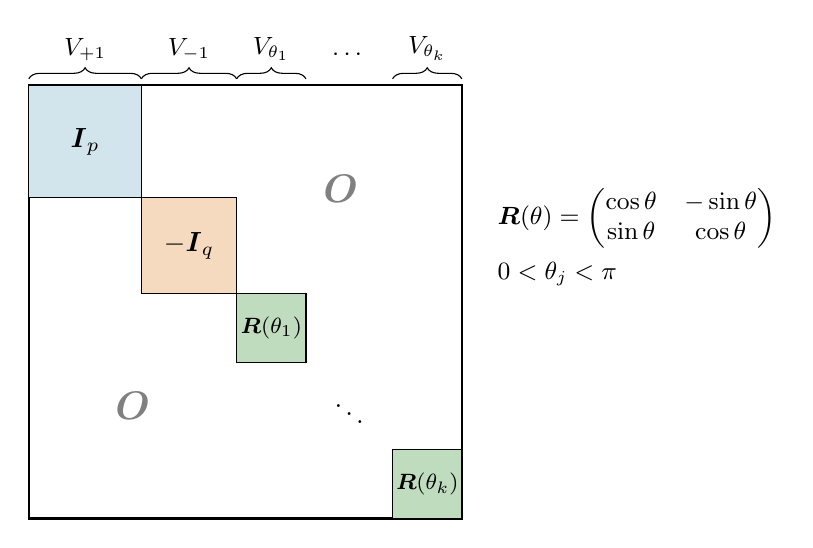
\begin{tikzpicture}[scale=0.55]
			\draw[thick] (0,0) rectangle (10,-10);
			\fill[figblue!25] (0,0) rectangle (2.6,-2.6);
			\fill[figorange!25] (2.6,-2.6) rectangle (4.8,-4.8);
			\fill[figgreen!25] (4.8,-4.8) rectangle (6.4,-6.4);
			\fill[figgreen!25] (8.4,-8.4) rectangle (10,-10);
			\foreach \a/\b in {0/2.6,2.6/4.8,4.8/6.4,8.4/10}{\draw (\a,-\a) rectangle (\b,-\b);}
			\node at (1.3,-1.3) {$\vv I_p$};
			\node at (3.7,-3.7) {$-\vv I_q$};
			\node[font=\footnotesize] at (5.6,-5.6) {$\vv R(\theta_1)$};
			\node at (7.4,-7.4) {$\ddots$};
			\node[font=\footnotesize] at (9.2,-9.2) {$\vv R(\theta_k)$};
			\node[gray,font=\Large] at (7.2,-2.4) {$\vv O$};
			\node[gray,font=\Large] at (2.4,-7.4) {$\vv O$};
			\draw[decorate,decoration={brace,amplitude=4pt}] (0,0.15) -- node[above=3pt,font=\small]{$V_{+1}$} (2.6,0.15);
			\draw[decorate,decoration={brace,amplitude=4pt}] (2.6,0.15) -- node[above=3pt,font=\small]{$V_{-1}$} (4.8,0.15);
			\draw[decorate,decoration={brace,amplitude=4pt}] (4.8,0.15) -- node[above=3pt,font=\small]{$V_{\theta_1}$} (6.4,0.15);
			\node[above=3pt,font=\small] at (7.4,0.15) {$\cdots$};
			\draw[decorate,decoration={brace,amplitude=4pt}] (8.4,0.15) -- node[above=3pt,font=\small]{$V_{\theta_k}$} (10,0.15);
			\node[right,align=left,font=\small] at (10.6,-3.5) {$\vv R(\theta)=\begin{pmatrix}\cos\theta&-\sin\theta\\ \sin\theta&\cos\theta\end{pmatrix}$\\[4pt] $0<\theta_j<\pi$};
		\end{tikzpicture}
		\caption{实正交变换的标准形. 在适当的标准正交基下，矩阵沿对角线分成三类块：不动（$1$）、翻转（$-1$）、二维旋转，每一块都至多二维.}
		\label{fig:orthcanon}
	\end{figure}
	\begin{remark}
		在这个分解中，$V_{+1}$ 与 $V_{-1}$ 是由 $\mathscr T$ 唯一确定的；角度 $\theta_1,\ldots,\theta_k$（连同重复）也是唯一的，因为特征多项式为
		\[f(\lambda)=(\lambda-1)^p(\lambda+1)^q\prod_{j=1}^k(\lambda^2-2\lambda\cos\theta_j+1),\]
		$\mathrm e^{\pm\mathrm i\theta_j}$ 恰好是 $\mathscr T$ 的非实复特征值. 但当某个角度重复出现时，旋转平面 $V_{\theta_j}$ 本身的选取不唯一：例如 $\mathbb{R}^4$ 中的 $\diag(\vv R(\theta),\vv R(\theta))$，可以有无穷多种方式拆成两个旋转平面.
	\end{remark}
	
	\begin{corollary}[欧拉旋转定理]\label{cor:euler}\index{ou1la1 xuan2zhuan3 ding4li3@欧拉旋转定理}
		设 $\vv Q$ 是三阶正交矩阵，$\det\vv Q=1$，$\vv Q\ne\vv I$. 则存在唯一的一条过原点的直线（\textbf{旋转轴}\index{xuan2zhuan3zhou2@旋转轴}）上的向量全部不动，$\vv Q$ 是绕这条轴、在与之垂直的平面内旋转角 $\theta$ 的变换，并且
		\[\cos\theta=\frac{\operatorname{tr}\vv Q-1}2.\]
	\end{corollary}
	\begin{proof}
		在结构定理中 $p+q+2k=3$，$\det\vv Q=(-1)^q=1$，故 $q$ 为偶数. 若 $k=1$，则 $p+q=1$，只能 $p=1$，$q=0$：一条不动的轴，加上与之垂直的旋转平面 $V_\theta$. 若 $k=0$，则 $(p,q)=(3,0)$ 或 $(1,2)$；前者 $\vv Q=\vv I$，已被排除；后者是绕 $V_{+1}$ 转角 $\pi$. 两种情形都有唯一的轴 $V_{+1}$. 最后，迹是相似不变量，$\operatorname{tr}\vv Q=1+2\cos\theta$.
	\end{proof}
	
	所以地球仪上那两个回到原处的点，就是旋转轴与球面的两个交点.
	
	\begin{example}
		$\vv Q=\begin{pmatrix}0&0&1\\1&0&0\\0&1&0\end{pmatrix}$ 把 $\vv e_1\mapsto\vv e_2\mapsto\vv e_3\mapsto\vv e_1$，它的列是标准正交的，$\det\vv Q=1$. 显然 $(1,1,1)^\trans$ 不动，旋转轴是 $V_{+1}=\spn\big((1,1,1)^\trans\big)$. $\operatorname{tr}\vv Q=0$，所以 $\cos\theta=-\frac12$，$\theta=\frac{2\pi}3$；旋转平面是轴的正交补 $\{x_1+x_2+x_3=0\}$.
		
		这里藏着第二章的一个老朋友：例~\ref{eg:pricedecomp} 中的``价格水平''直线 $L$ 与``相对价格''平面 $R$. 把三种商品的价格``轮换一下标签''，一般价格水平不变（$L$ 是旋转轴），相对价格结构则在 $R$ 中转了 $120^\circ$——转三次回到原样.
	\end{example}
	\begin{figure}[htbp]
		\centering
		\begin{tikzpicture}[iso2,scale=1.7]
			\def\R{1.22}
			\coordinate (O) at (0,0,0);
			\fill[figorange,opacity=0.13] (1.8,-0.6,-1.2) -- (0.6,-1.8,1.2) -- (-1.8,0.6,1.2) -- (-0.6,1.8,-1.2) -- cycle;
			\draw[figorange!70] (1.8,-0.6,-1.2) -- (0.6,-1.8,1.2) -- (-1.8,0.6,1.2) -- (-0.6,1.8,-1.2) -- cycle;
			\node[figorange,font=\small,anchor=north] at (1.5,-0.5,-1) {旋转平面 $x_1+x_2+x_3=0$};
			\draw[gray!70,dashed] plot[domain=0:360,samples=80] ({\R*(cos(\x)*0.7071+sin(\x)*0.4082)},{\R*(-cos(\x)*0.7071+sin(\x)*0.4082)},{\R*(-2*sin(\x)*0.4082)});
			\foreach \s/\e in {42/138,162/258,282/378}{
				\draw[->,thick,figred] plot[domain=\s:\e,samples=30] ({\R*(cos(\x)*0.7071+sin(\x)*0.4082)},{\R*(-cos(\x)*0.7071+sin(\x)*0.4082)},{\R*(-2*sin(\x)*0.4082)});
			}
			\draw[thick,figblue] (-0.9,-0.9,-0.9) -- (O);
			\draw[vec,figblue,line width=1.4pt] (O) -- (1.35,1.35,1.35) node[above,font=\small]{旋转轴 $(1,1,1)^\trans$};
			\draw[axis] (O) -- (1.5,0,0) node[below]{$\vv e_1$};
			\draw[axis] (O) -- (0,1.5,0) node[right]{$\vv e_2$};
			\draw[axis] (O) -- (0,0,1.5) node[above left]{$\vv e_3$};
			\foreach \t/\n in {30/1,150/2,270/3}{
				\node[dot,figviolet] (p\n) at ({\R*(cos(\t)*0.7071+sin(\t)*0.4082)},{\R*(-cos(\t)*0.7071+sin(\t)*0.4082)},{\R*(-2*sin(\t)*0.4082)}) {};
			}
			\node[figred,font=\small] at ($(p1)!0.5!(p2)+(0,0,0.45)$) {$120^\circ$};
		\end{tikzpicture}
		\caption{轮换矩阵 $\vv e_1\mapsto\vv e_2\mapsto\vv e_3\mapsto\vv e_1$ 是绕轴 $(1,1,1)^\trans$ 的旋转. 三个紫点是 $\vv e_1,\vv e_2,\vv e_3$ 在旋转平面上的投影，每作用一次就沿圆周转 $120^\circ$. 旋转轴与旋转平面恰好是图~\ref{fig:pricedecomp} 中的 $L$ 与 $R$.}
		\label{fig:eulerrotation}
	\end{figure}
	\begin{corollary}
		\begin{enumerate}
			\item 若 $\det\vv Q=-1$，则 $-1$ 是 $\vv Q$ 的特征值：总有一个方向被翻转.
			\item 若 $n$ 为奇数且 $\det\vv Q=1$，则 $1$ 是 $\vv Q$ 的特征值：奇数维空间中保持定向的正交变换总有不动的方向.
			\item 偶数维空间中则未必. $\mathbb{R}^4$ 中的 $\diag\big(\vv R(\theta_1),\vv R(\theta_2)\big)$（$0<\theta_1,\theta_2<\pi$）在两个互相垂直的平面里同时旋转，没有任何非零向量不动——\textbf{四维空间里的旋转可以没有轴}.
		\end{enumerate}
	\end{corollary}
	\begin{proof}
		(1) $(-1)^q=-1$，$q$ 为奇数，$q\ge1$. (2) $q$ 为偶数，$p=n-q-2k$ 为奇数，$p\ge1$. (3) 此时 $p=q=0$.
	\end{proof}
	
	\begin{historybox}{欧拉与刚体}
		1775 年，欧拉在研究刚体运动的论文\cite{euler1776formulae}中证明了：刚体绕一个固定点的任何运动，其结果都等价于绕过该点的某根轴的一次转动. 欧拉的证明是纯几何的——那时还没有矩阵，也没有特征值. 今天，这个定理是航天器姿态控制、三维动画和手机陀螺仪算法的基础：描述一个三维转动只需要一根轴和一个角度. 而本节的结构定理表明，欧拉定理只是``实多项式的不可约因式至多二次''在三维空间中投下的影子.
	\end{historybox}
	
	\begin{exercise}
		\begin{enumerate}
			\item 在 $\mathbb{R}^3$ 中求 $W=\spn((1,1,0)^\trans,(0,1,1)^\trans)$ 的正交补.
			\item 证明：在标准内积下，第二章例~\ref{eg:pricedecomp} 中的 $L$ 与 $R$ 互为正交补. 由此说明，把价格变动分解为``平均变动''与``偏离平均''，就是向 $L$ 作正交投影.
			\item 设 $W_1\subset W_2$，证明 $W_2^\perp\subset W_1^\perp$. 并证明 $(W_1+W_2)^\perp=W_1^\perp\cap W_2^\perp$.
			\item 设 $\mathscr P$ 是向 $W$ 的正交投影. 证明 $\mathscr P$ 是线性变换，$\mathscr P^2=\mathscr P$，$\ker\mathscr P=W^\perp$，$\imm\mathscr P=W$.
			\item\label{exo:ortho-rank} 用定理~\ref{thm:fourspaces} 证明 $\rk(\vv A^\trans\vv A)=\rk\vv A$，从而当 $\vv A$ 列满秩时正规方程有唯一解.
			\item 求 $\vv Q=\frac13\begin{pmatrix}2&-1&2\\2&2&-1\\-1&2&2\end{pmatrix}$ 的旋转轴与旋转角.
			\item 证明：平面上的旋转 $\vv R(\theta)$ 是两个反射之积. 由结构定理推出：$\mathbb{R}^n$ 上的每个正交变换都是至多 $n$ 个 Householder 反射之积（Cartan–Dieudonné 定理）.
			\item 设 $\vv Q$ 是正交矩阵. 证明：存在正整数 $m$ 使 $\vv Q^m=\vv I$，当且仅当结构定理中每个 $\theta_j$ 都是 $\pi$ 的有理数倍.
			\item 证明：若 $\mathscr T$ 是正交变换，则 $\ker(\mathscr T-\mathscr I)^\perp=\imm(\mathscr T-\mathscr I)$.
			\item （思考）引理~\ref{lem:orthinvperp} 的证明用到了什么？对于满足 $\langle\mathscr T\vv\alpha,\vv\beta\rangle=\langle\vv\alpha,\mathscr T\vv\beta\rangle$ 的变换，类似的结论是否成立？（第十章的谱定理会回答这个问题.）
		\end{enumerate}
	\end{exercise}
	\section{*范数与 \texorpdfstring{$\ell^p$}{lp}、\texorpdfstring{$L^p$}{Lp} 空间（选读）}\label{sec:lp}
	
	本节只用到第~\ref{sec:innerproduct}~节和高等数学中的定积分与级数，目的是让读者看到：本章的``长度''只是度量向量大小的一种方式，换一种度量方式，就会得到不同的几何与不同的应用. 本节的许多结论不加证明.
	
	\begin{motivebox}
		本章的长度 $\|\vv\alpha\|=\sqrt{\langle\vv\alpha,\vv\alpha\rangle}$ 来自内积. 但在实际问题中，度量``大小''或``误差''的方式不止一种. 比如在横平竖直的街区里，两点之间的步行距离是横向距离与纵向距离之和，而不是直线距离. 能不能撇开内积，直接规定什么是``长度''？
	\end{motivebox}
	
	\subsection{范数}
	
	\begin{definition}
		设 $V$ 是实向量空间. 若对每个 $\vv\alpha\in V$ 有一个实数 $\|\vv\alpha\|$ 与之对应，且对一切 $\vv\alpha,\vv\beta\in V$，$k\in\mathbb{R}$ 满足
		\begin{enumerate}
			\item （正定性）$\|\vv\alpha\|\ge0$，且 $\|\vv\alpha\|=0$ 当且仅当 $\vv\alpha=\zero$；
			\item （齐次性）$\|k\vv\alpha\|=|k|\,\|\vv\alpha\|$；
			\item （三角不等式）$\|\vv\alpha+\vv\beta\|\le\|\vv\alpha\|+\|\vv\beta\|$，
		\end{enumerate}
		则称 $\|\cdot\|$ 是 $V$ 上的一个\textbf{范数}\index{fan4shu4@范数}，配备了范数的向量空间称为\textbf{赋范空间}\index{fu4fan4 kong1jian1@赋范空间}(normed space).
	\end{definition}
	
	由第~\ref{sec:innerproduct}~节的 Cauchy–Schwarz 不等式及其推论，内积给出的长度满足这三条，所以它是范数. 反过来，范数不一定来自内积.
	
	\begin{definition}
		设 $p\ge1$. 对 $\vv x=(x_1,\ldots,x_n)^\trans\in\mathbb{R}^n$，令
		\[
		\|\vv x\|_p=\big(|x_1|^p+|x_2|^p+\cdots+|x_n|^p\big)^{1/p},\qquad \|\vv x\|_\infty=\max_{1\le i\le n}|x_i|.
		\]
		最常用的是三种：$\|\vv x\|_1=\sum|x_i|$，$\|\vv x\|_2=\sqrt{\sum x_i^2}$（即标准内积给出的长度），以及 $\|\vv x\|_\infty$.
	\end{definition}
	
	正定性与齐次性可以直接验证. $p=1$ 与 $p=\infty$ 时，三角不等式由实数的 $|a+b|\le|a|+|b|$ 逐分量得到；$p=2$ 时就是第~\ref{sec:innerproduct}~节的三角不等式. 一般的 $p\ge1$ 对应 \textbf{Minkowski 不等式}\index{minkowski bu4deng3shi4@Minkowski 不等式}，这里不作证明. 把 $p\to\infty$ 时的极限记为 $\|\vv x\|_\infty$，这也是记号的来由.
	
	\begin{pitfallbox}
		$0<p<1$ 时，$\|\cdot\|_p$ \textbf{不是}范数. 取 $p=\frac12$，$\vv x=(1,0)^\trans$，$\vv y=(0,1)^\trans$，则 $\|\vv x\|_p=\|\vv y\|_p=1$，而
		\[\|\vv x+\vv y\|_p=\big(1^{1/2}+1^{1/2}\big)^2=4>\|\vv x\|_p+\|\vv y\|_p,\]
		三角不等式不成立.
	\end{pitfallbox}
	
	\begin{figure}[htbp]
		\centering
		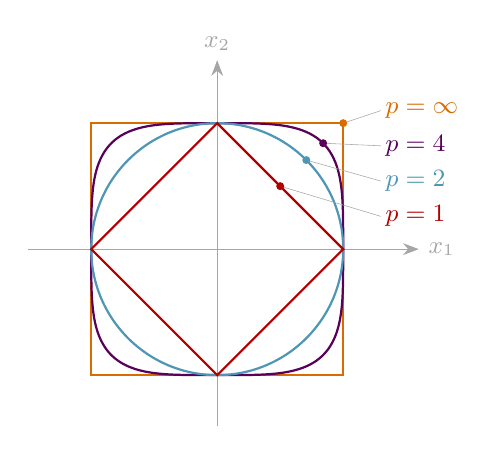
\begin{tikzpicture}[scale=1.6]
			\draw[axis] (-1.5,0) -- (1.6,0) node[right,font=\small]{$x_1$};
			\draw[axis] (0,-1.4) -- (0,1.5) node[above,font=\small]{$x_2$};
			\draw[thick,figorange] (-1,-1) rectangle (1,1);
			\draw[thick,figviolet,domain=0:360,samples=120,smooth]
			plot ({cos(\x)/((abs(cos(\x)))^4+(abs(sin(\x)))^4)^(0.25)},
			{sin(\x)/((abs(cos(\x)))^4+(abs(sin(\x)))^4)^(0.25)});
			\draw[thick,figblue] (0,0) circle (1);
			\draw[thick,figred] (1,0) -- (0,1) -- (-1,0) -- (0,-1) -- cycle;
			
			% 引线标注：曲线上 45° 处的点 -> 右侧一列标签
			\foreach \px/\lab/\ly/\col in {
				1/{p=\infty}/1.10/figorange,
				0.8409/{p=4}/0.82/figviolet,
				0.7071/{p=2}/0.54/figblue,
				0.5/{p=1}/0.26/figred}
			{
				\draw[gray!70,very thin] (\px,\px) -- (1.30,\ly);
				\fill[\col] (\px,\px) circle (0.9pt);
				\node[\col,font=\small,right,inner sep=1.5pt] at (1.30,\ly) {$\lab$};
			}
		\end{tikzpicture}
		\caption{$\mathbb{R}^2$ 中不同范数下的``单位圆'' $\{\vv x:\|\vv x\|_p=1\}$. $p$ 从 $1$ 增大到 $\infty$，单位圆从菱形逐渐变成正方形；只有 $p=2$ 时它是通常的圆.}
		\label{fig:lpballs}
	\end{figure}
	
	\paragraph*{有限维空间中的范数.} 由定义容易验证
	\[
	\|\vv x\|_\infty\le\|\vv x\|_2\le\|\vv x\|_1\le\sqrt n\,\|\vv x\|_2\le n\|\vv x\|_\infty.
	\]
	于是，若一列向量在其中一种范数下趋于零，在另外两种范数下也趋于零. 可以证明，有限维空间上的任意两个范数都有这样的关系（称为\textbf{等价}）. 因此在有限维空间中，选哪种范数不影响``收敛''与否，只影响具体的数值与几何形状.
	
	\paragraph*{哪些范数来自内积.} 第九章章末习题~\ref{ex:ip:B1} 说明，$\|\cdot\|_1$ 不满足\textbf{平行四边形法则}\index{ping2xing2 si4bian1xing2 fa3ze2@平行四边形法则}
	\[
	\|\vv\alpha+\vv\beta\|^2+\|\vv\alpha-\vv\beta\|^2=2\|\vv\alpha\|^2+2\|\vv\beta\|^2,
	\]
	因而不能来自任何内积. 一般地可以证明：一个范数来自某个内积，当且仅当它满足平行四边形法则. 在 $\|\cdot\|_p$ 中，只有 $p=2$ 满足. 换句话说，``角度''与``正交''是 $p=2$ 独有的结构，本章关于正交投影的全部结论都依赖于它.
	
	\begin{linkbox}{三种误差，三种答案}
		设对某个量做了 $n$ 次观测，得到 $y_1,\ldots,y_n$，希望用一个数 $c$ 来概括它们. 误差向量为 $\vv e=(y_1-c,\ldots,y_n-c)^\trans$，使哪种范数下的误差最小，就得到哪种``代表值''：
		\begin{itemize}
			\item 使 $\|\vv e\|_2$ 最小：$c$ 是\textbf{平均数}. 这是第九章最小二乘法最简单的情形.
			\item 使 $\|\vv e\|_1$ 最小：$c$ 是\textbf{中位数}. 把 $c$ 从左向右移动，每越过一个数据点，$\sum|y_i-c|$ 的斜率增加 $2$；斜率从负变为正的位置，正好是中间的那个数据点.
			\item 使 $\|\vv e\|_\infty$ 最小：$c$ 是最大值与最小值的平均，称为\textbf{中程数}.
		\end{itemize}
		对数据 $2,3,4,5,16$，三者分别为 $6$，$4$，$9$. 一个异常大的观测值 $16$，把平均数拉高了 $2$，把中程数拉高了更多，却完全不影响中位数. 这就是为什么统计学中有``最小一乘法''\index{zui4xiao3 yi1cheng2fa3@最小一乘法}：当数据中可能混有异常值时，用 $\|\cdot\|_1$ 度量误差，结论更稳健.
		
		$\ell^1$ 范数还有另一个用途. 在回归中把第十一章岭回归的惩罚项 $\mu\|\vv x\|_2^2$ 换成 $\mu\|\vv x\|_1$，所得的方法称为 LASSO. 由图~\ref{fig:lpballs} 可以想见：菱形的尖角落在坐标轴上，所以最优解往往有许多分量恰好为零. 这使 LASSO 能从大量候选变量中自动挑出少数几个，在计量经济学和数据科学中应用广泛. 选择哪一种范数，本质上是一个建模决定，而不是数学上的必然.
	\end{linkbox}
	
	\subsection{\texorpdfstring{$\ell^p$}{lp} 空间}
	
	把 $\mathbb{R}^n$ 中的向量换成无穷数列 $\vv a=(a_1,a_2,a_3,\ldots)$. 对 $p\ge1$，令
	\[
	\ell^p=\Big\{\vv a:\ \sum_{i=1}^\infty|a_i|^p<\infty\Big\},\qquad \|\vv a\|_p=\Big(\sum_{i=1}^\infty|a_i|^p\Big)^{1/p},
	\]
	并令 $\ell^\infty$ 为全体有界数列，$\|\vv a\|_\infty=\sup_i|a_i|$. 由 Minkowski 不等式（对前 $N$ 项成立，再令 $N\to\infty$），两个 $\ell^p$ 中数列之和仍在 $\ell^p$ 中，所以 $\ell^p$ 关于逐项的加法与数乘构成向量空间，$\|\cdot\|_p$ 是它上面的范数. 这样的空间称为 \textbf{$\ell^p$ 空间}\index{lp xu4lie4 kong1jian1@$\ell^p$ 空间}.
	
	与 $\mathbb{R}^n$ 不同，$\ell^p$ 是无限维的：第 $i$ 项为 $1$、其余项为 $0$ 的数列 $\vv e_1,\vv e_2,\ldots$ 中，任意有限个都线性无关. 无限维带来了有限维中没有的现象：
	\begin{itemize}
		\item \textbf{不同的 $p$ 给出不同的空间.} 若 $\sum|a_i|<\infty$，则 $a_i\to0$，从某项起 $|a_i|\le1$，于是 $a_i^2\le|a_i|$，故 $\ell^1\subset\ell^2$. 但 $\big(1,\frac12,\frac13,\ldots\big)$ 属于 $\ell^2$ 而不属于 $\ell^1$（调和级数发散），$(1,1,1,\ldots)$ 属于 $\ell^\infty$ 而不属于 $\ell^2$. 所以
		\[\ell^1\subsetneq\ell^2\subsetneq\ell^\infty.\]
		\item \textbf{范数不再等价.} 在有限维空间中，几种范数相差至多一个常数倍；在 $\ell^p$ 中，不存在这样的常数. 例如前 $N$ 项为 $\frac1{\sqrt N}$、其余为 $0$ 的数列，$\ell^2$ 范数恒为 $1$，$\ell^\infty$ 范数为 $\frac1{\sqrt N}\to0$，$\ell^1$ 范数为 $\sqrt N\to\infty$.
	\end{itemize}
	
	在这些空间中，只有 $\ell^2$ 有内积：$\langle\vv a,\vv b\rangle=\sum_{i=1}^\infty a_ib_i$. 由 Cauchy–Schwarz 不等式，这个级数总是绝对收敛的. 本章的标准正交基、正交投影、勾股定理，都可以推广到 $\ell^2$ 中，只是``有限和''要换成``级数''. 像 $\ell^2$ 这样具有内积、并且``没有缺口''（见下一小节）的空间，称为 \textbf{Hilbert 空间}\index{hilbert kong1jian1@Hilbert 空间}.
	
	\subsection{\texorpdfstring{$L^p$}{Lp} 空间}
	
	第九章已经在连续函数空间 $C[a,b]$ 上用积分定义了内积 $\langle f,g\rangle=\int_a^bf(x)g(x)\,\mathrm dx$，它给出的长度是 $\|f\|_2=\big(\int_a^b|f(x)|^2\,\mathrm dx\big)^{1/2}$. 仿照 $\ell^p$，对 $p\ge1$ 可以定义
	\[
	\|f\|_p=\Big(\int_a^b|f(x)|^p\,\mathrm dx\Big)^{1/p},\qquad \|f\|_\infty=\max_{a\le x\le b}|f(x)|.
	\]
	求和换成积分，数列的项换成函数在各点的值，这就是``函数是无穷维向量''的含义.
	
	然而，只用连续函数是不够的. 在 $[-1,1]$ 上取连续函数
	\[
	f_n(x)=\begin{cases}0,&x\le0,\\ nx,&0<x<\frac1n,\\ 1,&x\ge\frac1n,\end{cases}
	\qquad h(x)=\begin{cases}0,&x\le0,\\ 1,&x>0.\end{cases}
	\]
	计算可得 $\|f_n-h\|_2^2=\int_0^{1/n}(1-nx)^2\,\mathrm dx=\frac1{3n}\to0$：在 $\|\cdot\|_2$ 下，$f_n$ 越来越接近 $h$. 可是极限 $h$ 不是连续函数，它不在 $C[-1,1]$ 里. 这说明 $C[-1,1]$ 配上 $\|\cdot\|_2$ 是``有缺口''的：一列彼此越来越近的元素，其极限可能落在空间之外.
	
	补上这些缺口，需要比 Riemann 积分更一般的 Lebesgue 积分，并把在``可以忽略的集合''（例如有限个点）上取值不同的函数视为同一个元素. 补全之后的空间记为 $L^p[a,b]$，称为 \textbf{$L^p$ 空间}\index{lp han2shu4 kong1jian1@$L^p$ 空间}. 一个空间若没有上述缺口，就称为\textbf{完备的}\index{wan2bei4@完备}. $\ell^p$ 与 $L^p$ 都是完备的赋范空间，$\ell^2$ 与 $L^2$ 都是 Hilbert 空间. 严格的构造属于实变函数与泛函分析课程.
	
	在 $L^2[-\pi,\pi]$ 中，函数组 $1,\cos x,\sin x,\cos2x,\sin2x,\ldots$ 两两正交（第九章章末习题~\ref{ex:ip:B9}）. 一个函数的 \textbf{Fourier 级数}，正是它在这组正交函数上的``坐标展开''，而部分和就是它在有限个函数张成的子空间上的正交投影. 本章的最佳逼近定理在这里的含义是：在次数不超过 $N$ 的三角多项式中，Fourier 级数的前 $N$ 阶部分和在 $\|\cdot\|_2$ 下离原函数最近. 信号处理中把 $\|f\|_2^2$ 称为信号的``能量''，Fourier 展开把能量分配到各个频率上，这是勾股定理在无穷维中的推广.
	
	\begin{historybox}{从无穷多个未知数到泛函分析}
		二十世纪初，希尔伯特在研究积分方程时，把问题转化为``无穷多个未知数的线性方程组''，其中的未知数数列满足平方和有限，也就是今天的 $\ell^2$. 1907 年，希尔伯特的学生施密特（E.~Schmidt）给出了把线性无关组正交化的方法，1908 年，他在论文\cite{schmidt1908aufloesung}中为$\ell^2$建立了系统的几何语言. 1910 年，匈牙利数学家里斯（F.~Riesz）引入了 $L^p$ 空间\cite{riesz1910untersuchungen}. 波兰数学家巴拿赫（S.~Banach）在在 1920 年完成、1922 年发表的博士论文\cite{banach1922operations}中给出了完备赋范空间的公理化定义，这类空间后来以他的名字命名. 以这些空间为舞台研究线性映射的学科，称为\textbf{泛函分析}. 它可以看作把本书的线性代数推广到无穷维的结果.
	\end{historybox}
	
	\begin{exercise}
		\begin{enumerate}
			\item 对 $\vv x=(3,-4,0,1)^\trans$，计算 $\|\vv x\|_1$，$\|\vv x\|_2$，$\|\vv x\|_\infty$，并验证它们满足本节给出的不等式链.
			\item 证明：对 $\vv x\in\mathbb{R}^n$，$\|\vv x\|_\infty\le\|\vv x\|_2\le\sqrt n\,\|\vv x\|_\infty$，并说明两个等号分别在什么时候成立.
			\item 对数据 $1,2,2,3,12$，分别求使 $\|\vv e\|_1$，$\|\vv e\|_2$，$\|\vv e\|_\infty$ 最小的代表值 $c$. 若去掉 $12$，三个代表值各变化多少？
			\item 在 $\mathbb{R}^2$ 中取 $\vv\alpha=(1,0)^\trans$，$\vv\beta=(0,1)^\trans$，验证 $\|\cdot\|_\infty$ 不满足平行四边形法则.
			\item 判断数列 $\big(\frac1{\sqrt n}\big)$ 属于 $\ell^1$，$\ell^2$，$\ell^\infty$ 中的哪些.
		\end{enumerate}
	\end{exercise}
	\begin{codebox}{Gram–Schmidt 的数值陷阱}
		\mstep{目标} 实现 Gram–Schmidt 正交化，再在一个``难缠''的矩阵上，看它与数值软件的做法差多远.
		
		\mstep{准备} \texttt{numpy}；用于对照的 \texttt{numpy.linalg.qr}.
		
		\mstep{任务}
		\begin{enumerate}
			\item 按定理~\ref{thm:gramschmidt} 写函数 \texttt{gram\_schmidt(A)}，对矩阵的各列作正交化、单位化.
			\item 用本节例题的 $\vv\alpha_1,\vv\alpha_2,\vv\alpha_3$ 检验，并与 \texttt{qr} 给出的 $\vv Q$ 比较.
			\item 写函数 \texttt{modified\_gs(A)}：每得到一个新的单位向量 $\vv e_k$，就立即从\textbf{后面所有}列中减去它的分量.
			\item 构造 $10$ 阶 Hilbert 矩阵（$(i,j)$ 元为 $\frac1{i+j-1}$），用三种方法分别求 $\vv Q$，计算 $\|\vv Q^\trans\vv Q-\vv I\|$.
		\end{enumerate}
		
		\mstep{检查点} 例题：$\vv e_3=\frac1{\sqrt3}(-1,1,1)^\trans$；\texttt{qr} 给出的某些列与你的只差一个负号. Hilbert 矩阵：$\|\vv Q^\trans\vv Q-\vv I\|$ 依次约为 $3$、$10^{-4}$、$10^{-15}$.
		
		\mstep{思考}
		\begin{enumerate}
			\item 在精确运算下，三种方法给出完全相同的 $\vv Q$. 那么误差是从哪里来的？为什么相减的两个向量``几乎平行''时最危险？
			\item 对照本章的 Householder 反射，说明为什么正交变换不会放大舍入误差.
		\end{enumerate}
	\end{codebox}
	
	\ExInnerProduct
	
	\chapter{矩阵分解}
	% =====================================================================
	\paragraph*{本章地位}

	第八章讨论了矩阵的对角化，第九章引入了正交. 本章把二者结合起来，证明实对称矩阵可以用正交矩阵对角化（谱定理），即存在一组由特征向量构成的标准正交基. 在此基础上，本章对任意矩阵建立奇异值分解，由此得到矩阵的最佳低秩逼近，并讨论主成分分析等应用. 谱定理也是第十一章用正交变换化二次型为标准形的依据.
	
	\chapterhours{3}{5}{6}
	
	\begin{introduction}[学习目标]
		\item 说明实对称矩阵的特征值都是实数，属于不同特征值的特征向量互相正交
		\item 用正交矩阵把实对称矩阵对角化，写出谱分解
		\item 用 Rayleigh 商刻画实对称矩阵的最大与最小特征值（64 学时方案起）
		\item 求矩阵的奇异值分解，说明它的几何意义（64 学时方案起）
		\item 求矩阵的最佳低秩逼近，并用于主成分分析等问题（72 学时方案）
	\end{introduction}
	
	\paragraph*{前置知识}
	
	第八章（特征值与对角化）；第九章（标准正交基与正交矩阵）.
	
	\paragraph*{学习提示}
	\begin{itemize}
		\item 与第八章的对角化相比，谱定理多出的是正交性：对称矩阵的特征向量可以选成两两正交的. 这一性质使对称矩阵的计算与几何解释都大为简化.
		\item 奇异值分解把任意矩阵写成两个正交矩阵与一个对角矩阵的乘积，适用于一切矩阵，包括非方阵. 应注意区分奇异值与特征值.
		\item 本章的各项应用基于同一个思想：选取适合问题的标准正交基，使数据或变换的主要部分集中在少数几个方向上.
	\end{itemize}
	
	\newpage
	\begin{tcolorbox}[epigraph]
	\begin{quote}凡治众如治寡，分数是也；斗众如斗寡，形名是也.\end{quote}
	\begin{flushright}——《孙子兵法·兵势》\footnotemark\end{flushright}
	\end{tcolorbox}
	\footnotetext{``分数''指军队的分级编制，``形名''指旌旗、金鼓等指挥信号. 大意是：统率千军万马能像统率几个人一样，靠的是分层编组；指挥大军作战能像指挥小队一样，靠的是统一号令.}
	\section{实对称矩阵的谱定理}
	
	\begin{lemma}\label{lem:symreal}
		实对称矩阵的特征值都是实数.
	\end{lemma}
	\begin{proof}
		设 $\vv A$ 是实对称矩阵，$\lambda\in\mathbb{C}$，$\vv x\in\mathbb{C}^n$ 非零，$\vv{Ax}=\lambda\vv x$. 记 $\bar{\vv x}$ 为 $\vv x$ 的各分量取共轭，考虑数 $s=\bar{\vv x}^\trans\vv A\vv x$. 一方面 $s=\lambda\bar{\vv x}^\trans\vv x=\lambda\sum|x_i|^2$. 另一方面，由 $\vv A$ 是实矩阵且对称，
		\[\bar s=\vv x^\trans\vv A\bar{\vv x}=(\vv x^\trans\vv A\bar{\vv x})^\trans=\bar{\vv x}^\trans\vv A^\trans\vv x=\bar{\vv x}^\trans\vv A\vv x=s,\]
		所以 $s$ 是实数. 而 $\sum|x_i|^2>0$，故 $\lambda$ 是实数.
	\end{proof}
	
	于是 $\det(\lambda\vv I-\vv A)=0$ 的根都是实数，对每个特征值，$(\lambda\vv I-\vv A)\vv x=\zero$ 是实系数方程组，有\textbf{实}的非零解：实对称矩阵总有实特征向量.
	
	\begin{lemma}
		实对称矩阵属于不同特征值的特征向量互相正交.
	\end{lemma}
	\begin{proof}
		设 $\vv{Au}=\lambda\vv u$，$\vv{Av}=\mu\vv v$，$\lambda\ne\mu$. 则 $\lambda\vv u^\trans\vv v=(\vv{Au})^\trans\vv v=\vv u^\trans\vv A\vv v=\mu\vv u^\trans\vv v$，故 $\vv u^\trans\vv v=0$.
	\end{proof}
	
	\begin{theorem}[谱定理]\label{thm:spectral}\index{pu3 ding4li3@谱定理}
		对任意 $n$ 阶实对称矩阵 $\vv A$，存在正交矩阵 $\vv Q$ 使
		\[\vv Q^\trans\vv A\vv Q=\diag(\lambda_1,\ldots,\lambda_n),\]
		其中 $\lambda_i$ 是 $\vv A$ 的特征值. 换言之，$\mathbb{R}^n$ 有一组由 $\vv A$ 的特征向量构成的标准正交基. 反之，能被正交矩阵对角化的实矩阵一定是对称的.
	\end{theorem}
	\begin{proof}
		对 $n$ 归纳，$n=1$ 显然. 由引理~\ref{lem:symreal}，$\vv A$ 有实特征值 $\lambda_1$ 与单位实特征向量 $\vv q_1$. 由 Gram–Schmidt，把 $\vv q_1$ 扩充为 $\mathbb{R}^n$ 的标准正交基，以它们为列作正交矩阵 $\vv Q_1=(\vv q_1,\vv Q')$. 则
		\[\vv Q_1^\trans\vv A\vv Q_1=\begin{pmatrix}\vv q_1^\trans\vv A\vv q_1&\vv q_1^\trans\vv A\vv Q'\\ \vv Q'^\trans\vv A\vv q_1&\vv Q'^\trans\vv A\vv Q'\end{pmatrix}=\begin{pmatrix}\lambda_1&\zero^\trans\\ \zero&\vv B\end{pmatrix}.\]
		这里左下块 $\vv Q'^\trans(\lambda_1\vv q_1)=\zero$，因为 $\vv Q'$ 的列与 $\vv q_1$ 正交；整个矩阵是对称的，所以右上块也为零，且 $\vv B$ 是 $n-1$ 阶实对称矩阵. 由归纳假设，有 $n-1$ 阶正交矩阵 $\vv Q_2$ 使 $\vv Q_2^\trans\vv B\vv Q_2$ 为对角矩阵. 令 $\vv Q=\vv Q_1\diag(1,\vv Q_2)$，它是正交矩阵之积，仍是正交矩阵，且 $\vv Q^\trans\vv{AQ}$ 为对角矩阵.
		
		反之，若 $\vv A=\vv Q\vv D\vv Q^\trans$，则 $\vv A^\trans=\vv Q\vv D^\trans\vv Q^\trans=\vv A$.
	\end{proof}
	
	\begin{motivebox}
		把这个证明与第九章正交变换的结构定理并排放：两者都是``找到一个小的不变子空间，再证明它的正交补也不变，然后归纳''. 正交变换靠的是``保持内积''，对称矩阵靠的是 $\langle\vv{Ax},\vv y\rangle=\langle\vv x,\vv{Ay}\rangle$（这样的变换称为\textbf{自伴的}\index{zi4ban4 bian4huan4@自伴变换}）. 不同之处只在于：对称矩阵的小块总是一维的（特征值是实数），正交变换的小块可以是二维的（特征值可以是 $\mathrm e^{\pm\mathrm i\theta}$）.
	\end{motivebox}
	
	\paragraph*{正交对角化的步骤.} (1) 求出全部特征值；(2) 对每个特征值求特征子空间的基，并在\textbf{每个特征子空间内部}作 Gram–Schmidt 正交化、单位化；(3) 把所有这些向量排成 $\vv Q$. 不同特征子空间之间自动正交，无需再处理.
	
	\begin{example}
		例~\ref{eg:eig2112} 的 $\vv A=\begin{pmatrix}2&1\\1&2\end{pmatrix}$：取 $\vv Q=\frac1{\sqrt2}\begin{pmatrix}1&1\\-1&1\end{pmatrix}$，则 $\vv Q^\trans\vv{AQ}=\diag(1,3)$. $\vv Q$ 是旋转 $-45^\circ$：在旋转后的坐标系里，$\vv A$ 就是``沿一个轴不变、沿另一个轴放大三倍''.
	\end{example}
	
	把 $\vv Q=(\vv q_1,\ldots,\vv q_n)$ 按列展开，谱定理还可以写成
	\[\vv A=\vv Q\vv D\vv Q^\trans=\lambda_1\vv q_1\vv q_1^\trans+\lambda_2\vv q_2\vv q_2^\trans+\cdots+\lambda_n\vv q_n\vv q_n^\trans,\]
	称为\textbf{谱分解}\index{pu3 fen1jie3@谱分解}. 每个 $\vv q_i\vv q_i^\trans$ 是向 $\spn(\vv q_i)$ 的正交投影（第九章章末习题~\ref{ex:ip:A21}），所以：\textbf{对称矩阵就是若干个互相垂直方向上的投影，各自乘上一个伸缩倍数，再加起来.}
	
	\subsection{\hB 特征值的极值刻画}
	
	\begin{theorem}\label{thm:rayleigh}
		设实对称矩阵 $\vv A$ 的特征值为 $\lambda_1\ge\lambda_2\ge\cdots\ge\lambda_n$，对应的标准正交特征向量为 $\vv q_1,\ldots,\vv q_n$. 则
		\[\max_{\|\vv x\|=1}\vv x^\trans\vv{Ax}=\lambda_1,\qquad \min_{\|\vv x\|=1}\vv x^\trans\vv{Ax}=\lambda_n,\]
		最大值在 $\vv x=\pm\vv q_1$ 处取到，最小值在 $\vv x=\pm\vv q_n$ 处取到.
	\end{theorem}
	\begin{proof}
		把单位向量 $\vv x$ 写成 $\sum c_i\vv q_i$，则 $\sum c_i^2=1$，且
		\[\vv x^\trans\vv{Ax}=\sum_i\lambda_ic_i^2\le\lambda_1\sum_ic_i^2=\lambda_1,\]
		等号在 $\vv x=\pm\vv q_1$ 时成立. 最小值同理.
	\end{proof}
	
	量 $\dfrac{\vv x^\trans\vv{Ax}}{\vv x^\trans\vv x}$ 称为 \textbf{Rayleigh 商}\index{rayleigh shang1@Rayleigh 商}. 这个定理把``求特征值''变成了``求最大值''——下面的主成分分析正是从这里出发的.
	
	\section{\hB 奇异值分解}
	
	谱定理只对对称方阵成立. 对一般的 $m\times n$ 矩阵 $\vv A$，我们退一步：允许定义域和值域使用\textbf{两组不同的}标准正交基.
	
	\begin{motivebox}
		一个方阵把单位圆变成什么？对称矩阵把它变成一个椭圆，椭圆的轴恰好是特征向量的方向. 对一般矩阵，单位圆的像仍然是一个椭圆（高维时是椭球），但椭圆的轴\textbf{不一定}是原来某些向量的方向. 奇异值分解就是要同时找到：定义域中的哪组垂直方向，被变成了值域中椭圆的那组垂直的轴.
	\end{motivebox}
	
	\begin{theorem}[奇异值分解]\label{thm:svd}\index{qi2yi4zhi2 fen1jie3@奇异值分解}
		设 $\vv A$ 是 $m\times n$ 实矩阵，$\rk\vv A=r$. 则存在 $m$ 阶正交矩阵 $\vv U$、$n$ 阶正交矩阵 $\vv V$，以及 $\sigma_1\ge\sigma_2\ge\cdots\ge\sigma_r>0$，使
		\[\vv A=\vv U\vv\Sigma\vv V^\trans,\qquad \vv\Sigma=\begin{pmatrix}\diag(\sigma_1,\ldots,\sigma_r)&\vv O\\ \vv O&\vv O\end{pmatrix}_{m\times n}.\]
		$\sigma_i$ 称为 $\vv A$ 的\textbf{奇异值}\index{qi2yi4zhi2@奇异值}，它们是 $\vv A^\trans\vv A$ 的非零特征值的算术平方根. $\vv U$ 与 $\vv V$ 的列分别称为\textbf{左奇异向量}\index{zuo3 qi2yi4 xiang4liang4@左奇异向量}与\textbf{右奇异向量}\index{you4 qi2yi4 xiang4liang4@右奇异向量}.
	\end{theorem}
	\begin{proof}
		$\vv A^\trans\vv A$ 是 $n$ 阶实对称矩阵，且对任意 $\vv x$，$\vv x^\trans\vv A^\trans\vv A\vv x=\|\vv{Ax}\|^2\ge0$，所以它的特征值都非负. 由谱定理，取它的标准正交特征向量 $\vv v_1,\ldots,\vv v_n$，对应特征值 $\lambda_1\ge\cdots\ge\lambda_n\ge0$. 由于 $\rk(\vv A^\trans\vv A)=\rk\vv A=r$（第六章章末习题~\ref{ex:sol:B2}），恰有 $r$ 个特征值为正. 令 $\sigma_i=\sqrt{\lambda_i}$，并令
		\[\vv u_i=\frac1{\sigma_i}\vv A\vv v_i\qquad(i=1,\ldots,r).\]
		这些 $\vv u_i$ 两两正交且是单位向量：
		\[\vv u_i^\trans\vv u_j=\frac{\vv v_i^\trans\vv A^\trans\vv A\vv v_j}{\sigma_i\sigma_j}=\frac{\lambda_j\vv v_i^\trans\vv v_j}{\sigma_i\sigma_j}=\begin{cases}1,&i=j,\\0,&i\ne j.\end{cases}\]
		把 $\vv u_1,\ldots,\vv u_r$ 扩充为 $\mathbb{R}^m$ 的标准正交基 $\vv u_1,\ldots,\vv u_m$. 对 $i>r$，$\|\vv A\vv v_i\|^2=\lambda_i=0$，故 $\vv A\vv v_i=\zero$. 于是 $\vv A\vv v_i=\sigma_i\vv u_i$（$i\le r$），$\vv A\vv v_i=\zero$（$i>r$），即 $\vv{AV}=\vv U\vv\Sigma$. 右乘 $\vv V^\trans=\vv V^{-1}$ 即得.
	\end{proof}
	
	\paragraph*{几何意义.} $\vv A\vv x=\vv U\vv\Sigma\vv V^\trans\vv x$ 分三步：先用 $\vv V^\trans$ 做一次正交变换（把 $\vv v_i$ 转到坐标轴上），再用 $\vv\Sigma$ 沿坐标轴伸缩（第 $i$ 个轴伸缩 $\sigma_i$ 倍，多余的维数被压扁或补零），最后用 $\vv U$ 再做一次正交变换（把坐标轴转到 $\vv u_i$ 上）. 单位球的像是以 $\sigma_i\vv u_i$ 为半轴的椭球. 由第九章的结构定理，每个正交变换又只是若干平面旋转与反射的组合——于是\textbf{任何}线性映射都可以拆成``转、伸、转''.
	\begin{figure}[htbp]
		\centering
		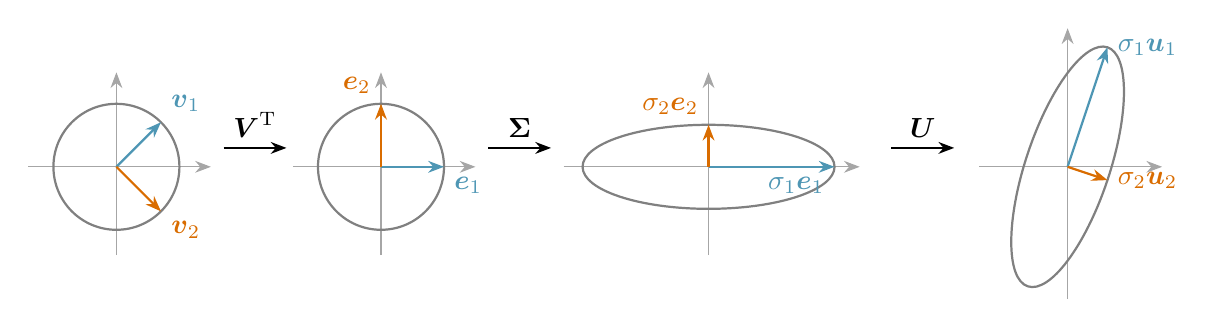
\begin{tikzpicture}[scale=0.8]
			\def\sa{2.0} \def\sb{0.667}
			% panel 1
			\begin{scope}
				\draw[axis] (-1.4,0) -- (1.5,0); \draw[axis] (0,-1.4) -- (0,1.5);
				\draw[thick,gray] (0,0) circle (1);
				\draw[vec,figblue] (0,0) -- (45:1) node[above right]{$\vv v_1$};
				\draw[vec,figorange] (0,0) -- (-45:1) node[below right]{$\vv v_2$};
			\end{scope}
			\draw[->,thick] (1.7,0.3) -- node[above]{$\vv V^\trans$} (2.7,0.3);
			% panel 2
			\begin{scope}[xshift=4.2cm]
				\draw[axis] (-1.4,0) -- (1.5,0); \draw[axis] (0,-1.4) -- (0,1.5);
				\draw[thick,gray] (0,0) circle (1);
				\draw[vec,figblue] (0,0) -- (1,0) node[below right]{$\vv e_1$};
				\draw[vec,figorange] (0,0) -- (0,1) node[above left]{$\vv e_2$};
			\end{scope}
			\draw[->,thick] (5.9,0.3) -- node[above]{$\vv\Sigma$} (6.9,0.3);
			% panel 3
			\begin{scope}[xshift=9.4cm]
				\draw[axis] (-2.3,0) -- (2.4,0); \draw[axis] (0,-1.4) -- (0,1.5);
				\draw[thick,gray] (0,0) ellipse [x radius=\sa, y radius=\sb];
				\draw[vec,figblue] (0,0) -- (\sa,0) node[below left]{$\sigma_1\vv e_1$};
				\draw[vec,figorange] (0,0) -- (0,\sb) node[above left]{$\sigma_2\vv e_2$};
			\end{scope}
			\draw[->,thick] (12.3,0.3) -- node[above]{$\vv U$} (13.3,0.3);
			% panel 4
			\begin{scope}[xshift=15.1cm]
				\draw[axis] (-1.4,0) -- (1.5,0); \draw[axis] (0,-2.1) -- (0,2.2);
				\draw[thick,gray,rotate=71.565] (0,0) ellipse [x radius=\sa, y radius=\sb];
				\draw[vec,figblue] (0,0) -- (71.565:\sa) node[right]{$\sigma_1\vv u_1$};
				\draw[vec,figorange] (0,0) -- (-18.435:\sb) node[right]{$\sigma_2\vv u_2$};
			\end{scope}
		\end{tikzpicture}
		\caption{奇异值分解 $\vv A=\vv U\vv\Sigma\vv V^\trans$：转、伸、转. 以 $\vv A=\begin{pmatrix}3&0\\4&5\end{pmatrix}$ 为例，$\sigma_1=3\sqrt5$，$\sigma_2=\sqrt5$；单位圆最终变成以 $\sigma_1\vv u_1$、$\sigma_2\vv u_2$ 为半轴的椭圆. 椭圆按 $\sigma_1:\sigma_2=3:1$ 的比例缩小画出.}
		\label{fig:svd}
	\end{figure}
	\begin{example}
		求 $\vv A=\begin{pmatrix}3&0\\4&5\end{pmatrix}$ 的奇异值分解.
	\end{example}
	\begin{solution}\textbf{}
		$\vv A^\trans\vv A=\begin{pmatrix}25&20\\20&25\end{pmatrix}$，特征值为 $45$ 与 $5$，对应单位特征向量 $\vv v_1=\frac1{\sqrt2}(1,1)^\trans$，$\vv v_2=\frac1{\sqrt2}(1,-1)^\trans$. 奇异值 $\sigma_1=3\sqrt5$，$\sigma_2=\sqrt5$. 再算
		\[\vv u_1=\frac{\vv A\vv v_1}{\sigma_1}=\frac1{\sqrt{10}}\begin{pmatrix}1\\3\end{pmatrix},\qquad \vv u_2=\frac{\vv A\vv v_2}{\sigma_2}=\frac1{\sqrt{10}}\begin{pmatrix}3\\-1\end{pmatrix}.\]
		所以 $\vv A=\vv U\diag(3\sqrt5,\sqrt5)\vv V^\trans$，$\vv U=(\vv u_1,\vv u_2)$，$\vv V=(\vv v_1,\vv v_2)$. 检验：$\sigma_1\sigma_2=15=|\det\vv A|$.
	\end{solution}
	
	\begin{pitfallbox}
		\begin{enumerate}
			\item 奇异值\textbf{不是}特征值. 上例中 $\vv A$ 的特征值是 $3$ 和 $5$，奇异值却是 $3\sqrt5\approx6.71$ 与 $\sqrt5\approx2.24$. 只有对称半正定矩阵，二者才一致.
			\item 不能分别对 $\vv A^\trans\vv A$ 与 $\vv A\vv A^\trans$ 独立求特征向量来拼出 $\vv U,\vv V$：特征向量的正负号（以及重特征值时的选取）必须配套. 稳妥的做法是先求 $\vv V$，再用 $\vv u_i=\vv A\vv v_i/\sigma_i$ 求 $\vv U$.
		\end{enumerate}
	\end{pitfallbox}
	
	\paragraph*{条件数.} 对可逆方阵，$\kappa(\vv A)=\sigma_1/\sigma_n$ 称为\textbf{条件数}：它是椭球最长轴与最短轴之比，衡量 $\vv A$ 把单位球``压扁''的程度. 第六章选读节的病态方程组，系数矩阵 $\begin{pmatrix}1&1\\1&1.0001\end{pmatrix}$ 的条件数约为 $4\times10^4$：右端的相对误差最多可能被放大四万倍. 行列式只反映体积，条件数才反映形状——这回答了第六章``常见误区''留下的问题.
	
	\section{\hC 低秩逼近}
	
	把 $\vv A=\vv U\vv\Sigma\vv V^\trans$ 按列展开，得
	\[\vv A=\sigma_1\vv u_1\vv v_1^\trans+\sigma_2\vv u_2\vv v_2^\trans+\cdots+\sigma_r\vv u_r\vv v_r^\trans,\]
	每一项都是秩为 $1$ 的矩阵，按``重要性''$\sigma_i$ 从大到小排列. 只保留前 $k$ 项，记为
	\[\vv A_k=\sigma_1\vv u_1\vv v_1^\trans+\cdots+\sigma_k\vv u_k\vv v_k^\trans.\]
	
	\begin{theorem}[Eckart–Young]\label{thm:eckartyoung}\index{eckart young ding4li3@Eckart–Young 定理}
		在所有秩不超过 $k$ 的 $m\times n$ 矩阵 $\vv B$ 中，$\vv A_k$ 离 $\vv A$ 最近：
		\[\|\vv A-\vv A_k\|_F\le\|\vv A-\vv B\|_F,\qquad \|\vv A-\vv A_k\|_F=\sqrt{\sigma_{k+1}^2+\cdots+\sigma_r^2},\]
		其中 $\|\vv M\|_F=\sqrt{\sum m_{ij}^2}$ 称为 \textbf{Frobenius 范数}\index{frobenius fan4shu4@Frobenius 范数}，它是第九章 $M_{m\times n}(\mathbb{R})$ 上的内积所对应的范数.
	\end{theorem}
	
	后一个等式容易验证：$\vv A-\vv A_k=\sum_{i>k}\sigma_i\vv u_i\vv v_i^\trans$，而各 $\vv u_i\vv v_i^\trans$ 在这个内积下两两正交、长度为 $1$（习题），由勾股定理即得. 前一个不等式（``最近''）的证明需要更多技巧，这里从略.
	
	\begin{motivebox}
		这个定理是第四章``图像压缩中的换基''的终极版本. 那里我们换了一组固定的基（亮度与色度），让重要的信息集中到少数坐标上；这里，SVD 为\textbf{每一个具体的矩阵}量身定做一组基，并且保证：在所有``只用 $k$ 个方向''的近似中，它是最好的.
	\end{motivebox}
	
	\section{\hC 应用：主成分分析与低秩近似}
	
	\subsection{主成分分析}\index{zhu3cheng2fen4 fen1xi1@主成分分析}
	
	设对 $n$ 个对象（地区、企业、个人）各观测了 $p$ 个指标，把数据排成 $n\times p$ 矩阵 $\vv X$，并假定每一列已经\textbf{中心化}（减去了该指标的均值）. 若给各指标分配权重 $\vv w\in\mathbb{R}^p$（$\|\vv w\|=1$），每个对象得到一个综合得分，所有得分组成向量 $\vv X\vv w$. 我们希望综合得分\textbf{尽可能地把各个对象区分开}，即让得分的方差
	\[\frac1{n-1}\|\vv X\vv w\|^2=\vv w^\trans\vv S\vv w,\qquad \vv S=\frac1{n-1}\vv X^\trans\vv X\]
	最大. $\vv S$ 是\textbf{样本协方差矩阵}\index{yang4ben3 xie2fang1cha1 ju3zhen4@样本协方差矩阵}，实对称且半正定. 由定理~\ref{thm:rayleigh}，最优的 $\vv w$ 是 $\vv S$ 最大特征值对应的单位特征向量，最大方差就是这个特征值. 这个方向称为\textbf{第一主成分}\index{zhu3cheng2fen4@主成分}；在与之正交的方向中再求方差最大者，得到第二主成分，依此类推——它们恰好是 $\vv S$ 的各个特征向量. 第 $i$ 个主成分``解释''了总方差的 $\lambda_i/\sum_j\lambda_j$.
	
	由 $\vv X^\trans\vv X=\vv V\vv\Sigma^\trans\vv\Sigma\vv V^\trans$，主成分方向就是 $\vv X$ 的右奇异向量. 实践中正是用 SVD 来计算主成分的，这在数值上比先算 $\vv X^\trans\vv X$ 更稳定.
	
	\begin{modelbox}{地区发展综合指数}
		\mstep{问题} 用三个指标——人均地区生产总值、居民人均可支配收入、每千人口卫生技术人员数——给若干地区编一个``发展综合指数''. 各指标应当如何加权？
		
		\mstep{假设} 各指标先\textbf{标准化}（减均值、除以标准差），以消除量纲的影响. 这时协方差矩阵就是\textbf{相关系数矩阵}\index{xiang1guan1 xi4shu4 ju3zhen4@相关系数矩阵}. 设由数据算得
		\[\vv R=\begin{pmatrix}1&0.8&0.6\\0.8&1&0.5\\0.6&0.5&1\end{pmatrix}.\]
		
		\mstep{求解} $\vv R$ 的特征值为 $2.275$，$0.536$，$0.189$（和为 $3=\operatorname{tr}\vv R$）. 第一主成分方向为
		\[\vv w_1\approx(0.616,\ 0.591,\ 0.521)^\trans,\]
		解释了 $2.275/3\approx75.8\%$ 的总方差. 把权重归一化使其和为 $1$，约为 $(0.356,\ 0.342,\ 0.302)$.
		
		\mstep{解读}
		\begin{itemize}
			\item 三个指标高度相关，一个综合指数就保留了四分之三的信息. 这是``降维''的正当理由.
			\item 主成分给出的权重与``等权重''$(\frac13,\frac13,\frac13)$ 相差不大，但并不相等：人均 GDP 权重最高，卫生人员权重最低. 原因是人均 GDP 与另外两个指标的相关性都最强.
		\end{itemize}
		
		\mstep{局限}
		\begin{itemize}
			\item 主成分的权重由\textbf{相关性}决定，而不是由\textbf{重要性}决定. 一个指标与其他指标越``同步''，权重就越大——这在某种意义上是在奖励冗余. 若政策上认为医疗资源与经济总量同等重要，主成分不会替你做出这个判断.
			\item 权重随数据变化：用今年的数据算出的权重，与去年的不同，两年的指数不能直接比较.
			\item 特征向量的符号不确定（$-\vv w_1$ 同样是解），解读前要检查方向是否符合常识.
		\end{itemize}
	\end{modelbox}
	
	\subsection{潜在语义分析}
	
	\begin{modelbox}{法条检索（续）：让``解约''找到``解除合同''}
		\mstep{问题} 第三章的词项—文档矩阵只能匹配\textbf{字面相同}的词. 当事人搜索``解约''，一份只写了``解除合同''的文书得分为零. 能否让系统``懂得''两者意思相近？
		
		\mstep{模型} 取一个极小的例子：六个词（合同、解除、解约、违约金、离婚、抚养），四份文书，$D_1$：合同、解除、违约金；$D_2$：合同、解约、违约金；$D_3$：合同、解除；$D_4$：离婚、抚养. 词项—文档矩阵为
		\[\vv A=\begin{pmatrix}1&1&1&0\\1&0&1&0\\0&1&0&0\\1&1&0&0\\0&0&0&1\\0&0&0&1\end{pmatrix}.\]
		对 $\vv A$ 作 SVD，只保留前 $k$ 个奇异值，用 $\vv U_k$ 的 $k$ 列作为``语义坐标轴''. 每份文书用 $\vv\Sigma_k\vv V_k^\trans$ 的对应列表示，查询 $\vv q$ 用 $\vv U_k^\trans\vv q$ 表示，再在这个 $k$ 维空间里算余弦相似度. 这种方法称为\textbf{潜在语义分析}\index{qian2zai4 yu3yi4 fen1xi1@潜在语义分析}（LSA）.
		
		\mstep{求解} 奇异值为 $2.474$，$1.414$，$1.252$，$0.559$. 查询``解约''$\vv q=\vv e_3$.
		\begin{itemize}
			\item 原始空间中，$\vv q$ 与四份文书的余弦相似度为 $(0,\ 0.577,\ 0,\ 0)$：只有 $D_2$ 字面上含``解约''.
			\item 取 $k=2$ 后，相似度变为 $(1,\ 1,\ 1,\ 0)$：$D_1$ 和 $D_3$ 虽然没有``解约''二字，却被认出与查询同属``合同纠纷''这一主题，而婚姻家庭类的 $D_4$ 仍为零.
		\end{itemize}
		由 Eckart–Young 定理，$\vv A_2$ 与 $\vv A$ 的距离为 $\sqrt{1.252^2+0.559^2}\approx1.371$.
		
		\mstep{解读} ``解约''与``解除''从未出现在同一份文书中，但它们都与``合同''``违约金''一起出现. 低秩近似迫使矩阵只用少数几个方向来描述全部文书，共现模式相似的词就被压到了相近的方向上. SVD 从数据中``发现''了同义关系，而没有人告诉它.
		
		\mstep{局限} 本例 $k=2$ 时，三份合同类文书的相似度全都变成了 $1$——压缩过了头，``解除''与``违约金''这样的区别也被抹平了. $k$ 取多少是一个权衡：太大则同义词连不起来，太小则不同的概念被混为一谈. 真实系统中词表有数万个词，$k$ 通常取几百. 今天的``词向量''和大语言模型中的``嵌入''，可以看作这一思想的远亲.
	\end{modelbox}
	
	\subsection{图像压缩}
	
	一张 $m\times n$ 的灰度图像就是一个 $m\times n$ 矩阵. 存储 $\vv A_k$ 只需要 $k$ 个奇异值、$k$ 个 $m$ 维向量和 $k$ 个 $n$ 维向量，共 $k(m+n+1)$ 个数，而原图需要 $mn$ 个数. 对 $1000\times1000$ 的图像取 $k=50$，存储量约为原来的十分之一. 自然图像的奇异值通常衰减得很快，前几十项就能保留轮廓与主要明暗；被丢掉的是细节和噪声. 下面的代码可以用任意一张照片做实验，请观察 $k=5,20,50$ 时的效果，并画出奇异值随序号衰减的曲线.
	
	\begin{historybox}{奇异值分解的百年}
		\sidefig[0.2\linewidth]{image/pearson.jpg}{卡尔·皮尔逊}[fig:pearson]
		1873 年与 1874 年，贝尔特拉米（E.~Beltrami）与若尔当（C.~Jordan）各自独立地得到了方阵的奇异值分解，当时是为了研究双线性型的化简\cite{beltrami1873funzioni,jordan1874memoire,stewart1993early}. 1901 年，统计学家皮尔逊（K.~Pearson）提出用``最贴近数据点的直线和平面''来概括数据\cite{pearson1901lines}，1933 年霍特林（H.~Hotelling）发展为主成分分析\cite{hotelling1933analysis}. 1936 年，心理测量学家埃卡特（C.~Eckart）与扬（G.~Young）证明了低秩逼近定理——他们关心的是如何从大量测验分数中提取少数几个``能力因子''\cite{eckart1936approximation}. 1960 年代，戈卢布（G.~Golub）等人给出了稳定高效的计算方法，SVD 才真正走进计算机\cite{golub1965calculating}.
	\end{historybox}
	
	\begin{codebox}{潜在语义分析的实现}
		\mstep{目标} 用截断 SVD 重做潜在语义分析，观察保留的维数 $k$ 怎样影响检索结果.
		
		\mstep{准备} \texttt{numpy.linalg.svd}；建模实验中的 $6\times4$ 词项—文档矩阵.
		
		\mstep{任务}
		\begin{enumerate}
			\item 输入词项—文档矩阵 $\vv A$，求奇异值分解.
			\item 写函数 \texttt{cosine(u, v)}，计算查询``解约''$\vv q=\vv e_3$ 在原始空间中与四份文书的余弦相似度.
			\item 写函数 \texttt{lsa\_scores(A, q, k)}：只保留前 $k$ 个奇异值，把文书表示为 $\vv\Sigma_k\vv V_k^\trans$ 的各列，把查询表示为 $\vv U_k^\trans\vv q$，再计算余弦相似度. 对 $k=1,2,3,4$ 各算一次，列成表.
			\item 计算 $\|\vv A-\vv A_2\|_F$，与定理~\ref{thm:eckartyoung} 给出的公式比较.
		\end{enumerate}
		
		\mstep{检查点} 奇异值约为 $2.474,1.414,1.252,0.559$；原始空间中的相似度为 $(0,0.577,0,0)$；$k=2$ 时为 $(1,1,1,0)$；$k=3$ 时约为 $(0.17,0.82,-0.20,0)$；$\|\vv A-\vv A_2\|_F\approx1.371$.
		
		\mstep{思考}
		\begin{enumerate}
			\item 从 $k=2$ 到 $k=3$，$D_2$ 的得分升高了，$D_1,D_3$ 的得分下降了. 第三个奇异向量``区分''了什么？你会选哪个 $k$？
			\item \texttt{svd} 返回的奇异向量可能与另一个软件差一个负号. 这会影响相似度的结果吗？为什么？
		\end{enumerate}
	\end{codebox}
	\section{*大语言模型中的线性代数（选读）}\label{sec:llm}
	
	\textbf{大语言模型}\index{da4 yu3yan2 mo2xing2@大语言模型}(large language model)是在海量文本上训练、能根据上文生成下文的程序. 它的内部细节很多，而且变化很快；但它的基本运算——向量的内积、矩阵乘法、低秩分解——几十年来没有变，正是本书的内容. 本节只讲这些稳定的部分：文字怎样变成向量，向量怎样经过一层层变换，以及怎样用低秩矩阵以很小的代价调整一个模型. 本节不追求完整，也不涉及训练的方法（那需要多元微积分与最优化）.
	
	\subsection{词元与嵌入}
	
	模型先把文本切分成\textbf{词元}\index{ci2yuan2@词元}(token)——字、词或词的一部分. 全体可能的词元构成词表，设其大小为 $N$，并给每个词元编号. 模型中有一个 $N\times d$ 矩阵 $\vv E$，第 $i$ 个词元对应 $\vv E$ 的第 $i$ 行，记为 $\vv e_i^\trans\vv E$，它是一个 $d$ 维向量，称为该词元的\textbf{嵌入}\index{qian4ru4@嵌入}(embedding). 实际模型中 $N$ 为数万到十几万，$d$ 为数千.
	
	$\vv E$ 的元素不是人为设定的，而是从数据中学出来的. 训练的结果是：在相近上下文中出现的词元，嵌入的方向也相近，可以用第九章的余弦相似度来度量. 这与本章潜在语义分析的想法一脉相承：在那里，SVD 把共现模式相似的词压到相近的方向上；在这里，同样的效果由训练得到，维数和数据规模大得多.
	
	2013 年，米科洛夫（T.~Mikolov）等人观察到，这类嵌入中存在近似的线性关系\cite{mikolov2013linguistic}：
	\[
	\text{嵌入}(\text{king})-\text{嵌入}(\text{man})+\text{嵌入}(\text{woman})
	\]
	与 $\text{嵌入}(\text{queen})$ 的余弦相似度最高. ``性别''在某种程度上对应于嵌入空间中的一个方向. 这种关系只是近似成立的，而且同样的机制也会把训练文本中的偏见编码进去，例如职业词与性别方向的关联. 在招聘、信贷、司法等场景中使用这类模型，需要检查并处理这种偏差.
	
	\subsection{线性层与非线性}
	
	模型的主体是许多``层''的叠加. 最基本的一层把向量 $\vv x\in\mathbb{R}^d$ 映为
	\[
	\vv y=\sigma(\vv W\vv x+\vv b),
	\]
	其中 $\vv W$ 是矩阵，$\vv b$ 是向量，$\sigma$ 是一个对每个分量分别作用的非线性函数，例如 $\sigma(t)=\max\{t,0\}$. 由这样的层组成的计算结构称为\textbf{神经网络}\index{shen2jing1 wang3luo4@神经网络}(neural network). 模型的``参数''，绝大部分就是这些矩阵的元素.
	
	为什么要有 $\sigma$？若去掉它，两层叠加得到
	\[
	\vv W_2(\vv W_1\vv x+\vv b_1)+\vv b_2=(\vv W_2\vv W_1)\vv x+(\vv W_2\vv b_1+\vv b_2),
	\]
	仍是``矩阵乘向量再加向量''的形式. 由定理~\ref{thm:composition}，线性映射的复合仍是线性映射，所以无论叠多少层，都只相当于一层. 非线性函数 $\sigma$ 打破了这一点，使多层网络能表示复杂得多的函数. 尽管如此，网络中几乎全部计算量都花在矩阵乘法上；专门为矩阵乘法设计的硬件（图形处理器等），是大模型得以训练的物质条件.
	
	\subsection{注意力机制}
	
	一句话中词的含义依赖于上下文. 例如``他把合同解除了''中``解除''的含义，要结合``合同''来理解. \textbf{注意力机制}\index{zhu4yi4li4 ji1zhi4@注意力机制}(attention)是让每个词元的向量吸收其他词元信息的方法.
	
	设一段文本有 $n$ 个词元，它们当前的向量作为行，排成 $n\times d$ 矩阵 $\vv X$. 用三个 $d\times d_k$ 的参数矩阵算出
	\[
	\vv Q=\vv X\vv W_Q,\qquad \vv K=\vv X\vv W_K,\qquad \vv V=\vv X\vv W_V.
	\]
	$\vv Q\vv K^\trans$ 的 $(i,j)$ 元是 $\vv Q$ 的第 $i$ 行与 $\vv K$ 的第 $j$ 行的内积，衡量第 $j$ 个词元与第 $i$ 个词元的相关程度. 对向量 $\vv z\in\mathbb{R}^n$，定义
	\[
	\operatorname{softmax}(\vv z)=\frac{1}{\sum_{j=1}^n\mathrm e^{z_j}}\big(\mathrm e^{z_1},\ldots,\mathrm e^{z_n}\big),
	\]
	它的分量都是正数，且和为 $1$. 注意力的输出是
	\[
	\operatorname{Attention}(\vv Q,\vv K,\vv V)=\vv P\vv V,\qquad \vv P=\operatorname{softmax}\Big(\frac{\vv Q\vv K^\trans}{\sqrt{d_k}}\Big),
	\]
	其中 softmax 对每一行分别作用. $\vv P$ 的每一行是一组非负、和为 $1$ 的权重，所以 $\vv P\vv V$ 的第 $i$ 行是 $\vv V$ 各行的\textbf{加权平均}：相关程度越高的词元，权重越大. 除以 $\sqrt{d_k}$ 是为了控制内积的大小：若两个向量的分量相互独立、均值为 $0$、方差为 $1$，它们的内积的方差是 $d_k$.
	
	\begin{example}
		取 $n=3$，$d=d_k=2$，$\vv X$ 的三行为 $(1,0)$，$(0,1)$，$(1,1)$，为简单起见令 $\vv W_Q=\vv W_K=\vv W_V=\vv I$，且不除以 $\sqrt{d_k}$. 则
		\[
		\vv Q\vv K^\trans=\vv X\vv X^\trans=\begin{pmatrix}1&0&1\\0&1&1\\1&1&2\end{pmatrix},
		\qquad
		\vv P\approx\begin{pmatrix}0.42&0.16&0.42\\0.16&0.42&0.42\\0.21&0.21&0.58\end{pmatrix},
		\]
		\[
		\vv P\vv V=\vv P\vv X\approx\begin{pmatrix}0.84&0.58\\0.58&0.84\\0.79&0.79\end{pmatrix}.
		\]
		第一个词元与自身、与第三个词元的内积都是 $1$，与第二个是 $0$，所以它主要吸收自身与第三个词元的信息. 输出的每一行都落在 $\vv X$ 三行所围成的三角形内. 若按实际做法除以 $\sqrt2$，第一行的权重变为约 $(0.40,0.20,0.40)$，分布更平均一些.
	\end{example}
	
	实际模型把 $\vv W_Q,\vv W_K,\vv W_V$ 的列分成若干块，每一块独立地做一次注意力，再把结果拼接起来，称为``多头注意力''——这就是第三章的分块矩阵. 一个大模型由几十层``注意力 $+$ 神经网络层''叠成，最后一层的输出乘以一个矩阵、再经过 softmax，得到词表上每个词元作为下一个词元的概率. 生成文本，就是反复按这个概率选取下一个词元.
	
	\subsection{低秩微调}
	
	训练一个大模型需要巨大的计算量. 想让它适应某个专门领域（比如法律文书），可以在已有参数的基础上做小幅修改，称为微调. 若把一个 $d\times d$ 的参数矩阵 $\vv W$ 改为 $\vv W+\Delta\vv W$，直接修改要调整 $d^2$ 个数. \textbf{低秩微调}\index{di1zhi4 wei1tiao2@低秩微调}(low-rank adaptation，LoRA)\cite{hu2022lora} 限定
	\[
	\Delta\vv W=\vv B\vv A,\qquad \vv B\in\mathbb{R}^{d\times r},\ \vv A\in\mathbb{R}^{r\times d},\ r\ll d.
	\]
	由第三章，$\rk(\vv B\vv A)\le r$. 需要调整的数只有 $2dr$ 个. 当 $d=4096$，$r=8$ 时，直接修改要调整 $4096^2=16\,777\,216$ 个数，而低秩微调只要 $2\times4096\times8=65\,536$ 个，约为前者的 $0.39\%$.
	
	这种做法有效的前提是：适应新领域所需的修改，本身近似是低秩的. 反过来，任何秩不超过 $r$ 的 $d\times d$ 矩阵都能写成 $\vv B\vv A$ 的形式（由奇异值分解，秩为 $s\le r$ 的矩阵等于 $\sum_{i=1}^{s}\sigma_i\vv u_i\vv v_i^\trans$，取 $\vv B$ 的前 $s$ 列为 $\sigma_i\vv u_i$，$\vv A$ 的前 $s$ 行为 $\vv v_i^\trans$，其余补零）；而由 Eckart–Young 定理（定理~\ref{thm:eckartyoung}），若修改量的奇异值衰减得快，用秩 $r$ 的矩阵逼近它损失很小. 本章的图像压缩与这里是同一个原理.
	
	\begin{linkbox}{模型会``编造''}
		大语言模型输出的是``在训练数据中看起来合理''的文本，而不是经过核实的事实. 它可能写出格式完整、却并不存在的判例、法条或文献. 2023 年，美国一家联邦法院在一起案件中处罚了提交由聊天机器人编造的判例引证的律师. 对法律工作而言，模型生成的每一条引证、每一个案号，都必须回到原始数据库中核对. 这与本书各章``局限''一节的要求相同：计算结果可以帮助思考，不能代替核实.
	\end{linkbox}
	
	\begin{historybox}{从词向量到 Transformer}
		用低维向量表示词语的想法，可以追溯到潜在语义分析（1990 年前后）. 2013 年，米科洛夫等人提出的 word2vec 方法能在大规模语料上快速训练词嵌入\cite{mikolov2013linguistic}. 2017 年，瓦斯瓦尼（A.~Vaswani）等人的论文《注意力就是你所需要的一切》提出了完全基于注意力机制的 Transformer 结构\cite{vaswani2017attention}，此后的大语言模型大多以它为基础. 2021 年，胡（E.~J.~Hu）等人提出了低秩微调\cite{hu2022lora}. 这一领域发展很快，本节提到的具体结构与规模都可能过时，但其中的矩阵运算不会.
	\end{historybox}
	
	\begin{codebox}{一个注意力层}
		\mstep{目标} 用十几行代码实现注意力机制，验证本节的例题.
		
		\mstep{准备} \texttt{numpy}. 实现 softmax 时，先把得分矩阵的每一行减去该行的最大值，再取指数、按行归一化.
		
		\mstep{任务}
		\begin{enumerate}
			\item 实现函数 \texttt{attention(Q, K, V)}，用本节例题检验（分别在除以与不除以 $\sqrt{d_k}$ 时）.
			\item 随机生成 $n=5$，$d=4$ 的 $\vv X$ 与三个参数矩阵，验证 $\vv P$ 的每行之和为 $1$.
			\item 把 $\vv X$ 的各行换一个顺序，输出的各行怎样变化？
			\item 取 $d=1024$，随机生成 $\vv B$（$d\times4$）与 $\vv A$（$4\times d$），用 \texttt{numpy.linalg.matrix\_rank} 验证 $\vv B\vv A$ 的秩.
		\end{enumerate}
		
		\mstep{检查点} 例题中 $\vv P$ 的第一行约为 $(0.42,0.16,0.42)$，除以 $\sqrt2$ 后约为 $(0.40,0.20,0.40)$；任务 4 的秩为 $4$.
		
		\mstep{思考}
		\begin{enumerate}
			\item 准备中的 softmax 写法为什么要先减去每行的最大值？结果会变吗？
			\item 任务 3 的结果说明，单靠注意力机制无法区分词元的先后顺序. 实际模型是怎样弥补这一点的？（可查阅``位置编码''.）
		\end{enumerate}
	\end{codebox}
	
	\begin{exercise}\label{exo:llm}
		\begin{enumerate}
			\item 对 $d=1024$，$r=4$，比较直接修改一个 $d\times d$ 参数矩阵与低秩微调需要调整的参数个数.
			\item 设 $\vv W_1$ 为 $h\times d$ 矩阵，$\vv W_2$ 为 $d\times h$ 矩阵. 不含非线性函数的两层 $\vv x\mapsto\vv W_2(\vv W_1\vv x+\vv b_1)+\vv b_2$ 等价于一层. 若 $h<d$，这个等价的单层的矩阵的秩至多是多少？
			\item 证明：若 $\vv P$ 的每行元素非负且和为 $1$，则 $\vv P\vv V$ 的每一行的每个分量，都介于 $\vv V$ 对应列的最小值与最大值之间. 若某一行的所有得分相等，输出是什么？
			\item 证明余弦相似度在把向量乘以正数时不变. 为什么比较嵌入时常用余弦相似度而不是内积？
			\item 证明：秩为 $r$ 的 $m\times n$ 矩阵都能写成 $\vv B\vv A$ 的形式，其中 $\vv B$ 为 $m\times r$ 矩阵，$\vv A$ 为 $r\times n$ 矩阵.
		\end{enumerate}
	\end{exercise}
	
	\newpage
	\ExDecomposition
	
	% =====================================================================
	\chapter*{第二部分综合项目}
	\addcontentsline{toc}{chapter}{第二部分综合项目}
	\markboth{第二部分综合项目}{第二部分综合项目}
	
	要求同第一部分：3—4 人一组，任选其一，两到三周完成，提交不超过 8 页的报告与可复现的代码，``局限''一节与计算结果同等重要. 选择过第一部分项目二、项目三的小组，鼓励在原有数据上继续. 评分按第一部分综合项目末尾的评分量规（第~\pageref{sec:rubric}~页）进行. 检查点：项目一须报告 $d$ 取三个值时的完整得分表并验证各得分之和为 $1$；项目二须画出奇异值衰减曲线；项目三须报告各主成分的解释方差比例与载荷.
	
	\section*{项目一：判例排序（接第一部分项目二）}
	\begin{enumerate}
		\item 在第一部分建立的引证网络上实现 PageRank，取阻尼系数 $d=0.5,\ 0.85,\ 0.95$，比较排序结果的变化.
		\item 与被引次数排序比较，找出排名变化最大的三份判决，结合案情解释原因.
		\item 设计一种``个性化''的随机跳转向量（例如偏向指导性案例或上级法院判决），讨论这种设计背后的价值判断.
		\item 尝试给否定性引用赋予较小的权重，讨论此时转移矩阵还满足哪些性质、不满足哪些性质.
	\end{enumerate}
	
	\section*{项目二：法条检索 2.0（接第一部分项目三）}
	\begin{enumerate}
		\item 在原有的词项—文档矩阵上，用余弦相似度代替共同词数，重新评价 5 个查询的结果.
		\item 对矩阵作截断 SVD，取 $k=5,10,20$，比较检索结果. 找出至少一个``字面不匹配、语义匹配''的成功例子和一个``被错误合并''的失败例子.
		\item 画出奇异值随序号衰减的曲线，讨论 $k$ 应当如何选取.
	\end{enumerate}
	
	\section*{项目三：一个综合指数}
	\begin{enumerate}
		\item 从国家统计局或各省统计年鉴的公开数据中，选取 30 个左右地区、5—8 个反映同一主题（如营商环境、公共服务、数字经济）的指标.
		\item 标准化后作主成分分析，报告各主成分的解释方差比例与载荷，给第一（或前两个）主成分一个有意义的名字.
		\item 把主成分权重与等权重、专家打分权重三种指数的排名放在一起比较，讨论三种做法各自的合理性与问题.
		\item 讨论：哪些指标``天然地''会得到高权重？这在政策评价中意味着什么？
	\end{enumerate}
	
	\begin{note}
		使用公开数据时，请遵守数据来源网站的使用条款，并在报告中注明来源. 涉及裁判文书的，注意对当事人信息作匿名化处理.
	\end{note}
	
	% =====================================================================
	\part{二次型}
	
	% =====================================================================
	\chapter{二次型}\label{ch:quadratic}
		
	\paragraph*{本章地位}
	
	此前，矩阵主要作为线性变换出现. 本章研究矩阵的另一种角色，即二次型：以向量为自变量、取值为各分量的二次齐次式的函数. 本章讨论如何通过可逆的变量替换把二次型化为只含平方项的标准形，证明标准形中正、负系数的个数与化法无关（惯性定理），并给出判别正定性的方法. 二次型出现在多元函数的极值、最小二乘法与投资组合风险等问题中.
	
	\chapterhours{5}{7}{7}
	
	\begin{introduction}[学习目标]
		\item 写出二次型的矩阵，判断两个实对称矩阵是否合同
		\item 用正交变换法与配方法把二次型化为标准形，判断二次曲线、二次曲面的类型
		\item 求二次型的正、负惯性指数与规范形
		\item 用特征值或顺序主子式判断二次型是否正定
		\item 用 Hessian 矩阵判断多元函数驻点的类型
		\item 把投资组合的方差写成二次型，求最小方差组合（64 学时方案起）
	\end{introduction}
	
	\paragraph*{前置知识}
	
	第五章（行列式与子式）；第十章（实对称矩阵的谱定理）；高等数学中多元函数的极值.
	
	\paragraph*{学习提示}
	\begin{itemize}
		\item 同一个实对称矩阵，作为二次型与作为线性变换时换基的规则不同：前者是合同，后者是相似. 二者只在正交变换下一致，这是正交变换法能够同时适用于两种情形的原因.
		\item 二次型的标准形不唯一，但正、负惯性指数不变. 判断二次型的性质时，应关注这些不变量，而不是某一种具体的化法.
		\item 正定性有多种等价的判别方法，包括特征值、惯性指数、合同关系与顺序主子式. 应根据具体问题选择最简便的一种.
	\end{itemize}
	
	\newpage
	
	\begin{tcolorbox}[epigraph]
	\begin{quote}We next consider the rule that the investor does (or should) consider expected return a desirable thing and variance of return an undesirable thing.\end{quote}
	\begin{flushright}——Harry Markowitz, \textit{Portfolio Selection}\end{flushright}
	\begin{quote}接下来我们考虑这样一条准则：投资者（实际上或者应当）把期望收益视为好东西，把收益的方差视为坏东西.\end{quote}
	\begin{flushright}——哈里·马科维茨\footnotemark\end{flushright}
	\end{tcolorbox}
	\footnotetext{哈里·马科维茨（1927—2023），美国经济学家，现代投资组合理论的奠基人，1990 年诺贝尔经济学奖得主之一. 引文出自其论文《投资组合选择》（\textit{Journal of Finance} 7 (1952), 77--91）的开篇. 组合收益的方差正是权重向量的一个二次型 $\vv w^\trans\vv\Sigma\vv w$——这是本章的贯穿案例.}
	
	\section{二次型及其矩阵}
	
	\subsection{从平面二次曲线出发}
	
	中学里，方程 $\frac{x^2}{a^2}+\frac{y^2}{b^2}=1$ 是椭圆，$\frac{x^2}{a^2}-\frac{y^2}{b^2}=1$ 是双曲线. 可是 $5x^2+4xy+2y^2=6$ 是什么曲线？交叉项 $4xy$ 让我们无从下手. 直觉告诉我们：也许把坐标轴转一个角度，交叉项就消失了. 本章把这个直觉变成一般的理论.
	
	\begin{definition}
		数域 $\mathbb{F}$ 上 $n$ 个变量的二次齐次多项式
		\[
		f(x_1,\ldots,x_n)=\sum_{i=1}^na_{ii}x_i^2+\sum_{1\le i<j\le n}2a_{ij}x_ix_j
		\]
		称为 $\mathbb{F}$ 上的 $n$ 元\textbf{二次型}\index{er4ci4xing2@二次型}(quadratic form). 令 $a_{ji}=a_{ij}$（$i<j$），得到对称矩阵 $\vv A=(a_{ij})$，于是
		\[f(\vv x)=\vv x^\trans\vv A\vv x.\]
		称 $\vv A$ 为二次型 $f$ 的\textbf{矩阵}，$\rk\vv A$ 称为二次型的\textbf{秩}. 本章除特别说明外，都在实数域上讨论.
	\end{definition}
	
	交叉项 $x_ix_j$ 的系数被\textbf{平分}到 $(i,j)$ 与 $(j,i)$ 两个位置上. 例如
	\[
	5x^2+4xy+2y^2=(x,y)\begin{pmatrix}5&2\\2&2\end{pmatrix}\begin{pmatrix}x\\y\end{pmatrix}.
	\]
	
	\begin{proposition}
		二次型与它的对称矩阵一一对应：若 $\vv A,\vv B$ 都是对称矩阵，且对一切 $\vv x$ 有 $\vv x^\trans\vv A\vv x=\vv x^\trans\vv B\vv x$，则 $\vv A=\vv B$.
	\end{proposition}
	\begin{proof}
		令 $\vv C=\vv A-\vv B$，它对称且 $\vv x^\trans\vv C\vv x\equiv0$. 取 $\vv x=\vv e_i$ 得 $c_{ii}=0$；取 $\vv x=\vv e_i+\vv e_j$ 得 $c_{ii}+2c_{ij}+c_{jj}=0$，故 $c_{ij}=0$.
	\end{proof}
	
	\begin{pitfallbox}
		不要求对称时，同一个二次型可以写成许多矩阵：$4xy$ 既是 $(x,y)\begin{pmatrix}0&4\\0&0\end{pmatrix}\binom xy$，也是 $(x,y)\begin{pmatrix}0&1\\3&0\end{pmatrix}\binom xy$. 只有约定``用对称矩阵''，``二次型的矩阵''才是良定义的. 一般地，$\vv x^\trans\vv M\vv x=\vv x^\trans\frac{\vv M+\vv M^\trans}2\vv x$，只有 $\vv M$ 的对称部分起作用.
	\end{pitfallbox}
	
	\subsection{变量替换与合同}
	
	把转轴写成代数语言，就是作可逆的线性变量替换 $\vv x=\vv C\vv y$（$\vv C$ 可逆）. 代入得
	\[
	f=\vv x^\trans\vv A\vv x=(\vv C\vv y)^\trans\vv A(\vv C\vv y)=\vv y^\trans(\vv C^\trans\vv A\vv C)\vv y.
	\]
	$\vv C^\trans\vv A\vv C$ 仍是对称矩阵，它就是新变量下二次型的矩阵.
	
	\begin{definition}
		若存在可逆矩阵 $\vv C$ 使 $\vv B=\vv C^\trans\vv A\vv C$，称 $\vv A$ 与 $\vv B$ \textbf{合同}\index{he2tong2@合同（矩阵）}(congruent).
	\end{definition}
	
	合同是等价关系（反身、对称、传递的验证与相似完全类似）. 由推论~\ref{cor:rankinvariant}，合同的矩阵秩相同，所以\textbf{二次型的秩不随可逆变量替换而改变}.
	
	\begin{pitfallbox}
		合同 $\vv C^\trans\vv A\vv C$ 与相似 $\vv P^{-1}\vv A\vv P$ 是两回事. $\diag(1,4)$ 与 $\vv I_2$ 合同（取 $\vv C=\diag(1,\frac12)$），却不相似（特征值不同）. 二次型 $x^2+4y^2$ 换成 $y'=2y$ 后就是 $x^2+y'^2$——作为``数值''，它们只是同一个函数用不同的尺子量；而作为``变换''，``拉伸 $4$ 倍''与``不动''当然不同. 为什么同一个对称矩阵会有两种换基规则？第十二章会给出答案. 两者唯一重合的情形是 $\vv C$ 为正交矩阵：$\vv C^\trans=\vv C^{-1}$.
	\end{pitfallbox}
	
	\section{化二次型为标准形}
	
	只含平方项的二次型 $d_1y_1^2+\cdots+d_ny_n^2$ 称为\textbf{标准形}\index{biao1zhun3xing2@标准形（二次型的）}，它的矩阵是对角矩阵. 化标准形，就是找可逆矩阵 $\vv C$ 使 $\vv C^\trans\vv A\vv C$ 为对角矩阵. 有两种方法.
	
	\subsection{正交变换法}
	
	\begin{theorem}[主轴定理]\label{thm:principalaxes}\index{zhu3zhou2 ding4li3@主轴定理}
		任一实二次型 $f=\vv x^\trans\vv A\vv x$ 都可以经过\textbf{正交变换} $\vv x=\vv Q\vv y$ 化为标准形
		\[f=\lambda_1y_1^2+\lambda_2y_2^2+\cdots+\lambda_ny_n^2,\]
		其中 $\lambda_1,\ldots,\lambda_n$ 是 $\vv A$ 的全部特征值，$\vv Q$ 的列是对应的标准正交特征向量.
	\end{theorem}
	\begin{proof}
		由谱定理（定理~\ref{thm:spectral}），有正交矩阵 $\vv Q$ 使 $\vv Q^\trans\vv A\vv Q=\diag(\lambda_1,\ldots,\lambda_n)$.
	\end{proof}
	
	正交变换保持长度与夹角（定理~\ref{thm:orthequiv}），所以它只是把坐标系\textbf{转了一下}（或再加一次反射），图形的形状和大小都不变. $\vv Q$ 的各列给出的方向称为二次型的\textbf{主轴}\index{zhu3zhou2@主轴}.
	
	\begin{example}\label{eg:ellipse}
		判断曲线 $5x^2+4xy+2y^2=6$ 的形状.
	\end{example}
	\begin{solution}
		$\vv A=\begin{pmatrix}5&2\\2&2\end{pmatrix}$，$\operatorname{tr}\vv A=7$，$\det\vv A=6$，特征值为 $6$ 与 $1$，对应单位特征向量
		\[\vv q_1=\tfrac1{\sqrt5}(2,1)^\trans,\qquad\vv q_2=\tfrac1{\sqrt5}(1,-2)^\trans.\]
		令 $(x,y)^\trans=u\vv q_1+v\vv q_2$，方程化为 $6u^2+v^2=6$，即
		\[u^2+\frac{v^2}{6}=1.\]
		这是一个椭圆：沿 $\vv q_1$ 方向（与 $x$ 轴夹角 $\arctan\frac12\approx26.6^\circ$）的半轴长为 $1$，沿与之垂直的 $\vv q_2$ 方向的半轴长为 $\sqrt6\approx2.45$. 特征值\textbf{越大}，那个方向上的半轴\textbf{越短}——曲线在那个方向上``爬得快''.
	\end{solution}
	
	\begin{figure}[htbp]
		\centering
		\begin{tikzpicture}[scale=0.72]
			% (a) ellipse 5x^2+4xy+2y^2=6
			\begin{scope}
				\draw[axis] (-2.8,0) -- (2.9,0) node[right,font=\small]{$x$};
				\draw[axis] (0,-2.7) -- (0,2.8) node[above,font=\small]{$y$};
				\draw[gray!60,dashed] (206.565:2.9) -- (26.565:2.9);
				\draw[gray!60,dashed] (116.565:2.9) -- (-63.435:2.9);
				\draw[thick,figblue,rotate=26.565] (0,0) ellipse [x radius=1, y radius=2.449];
				\draw[vec,figred] (0,0) -- (26.565:1) node[above right,font=\small]{$\vv q_1$};
				\draw[vec,figorange] (0,0) -- (-63.435:2.449) node[right,font=\small]{$\sqrt6\,\vv q_2$};
				\node[sub] at (0,-3.4) {(a) $5x^2+4xy+2y^2=6$\\正定：椭圆};
			\end{scope}
			% (b) hyperbola
			\begin{scope}[xshift=7cm]
				\draw[axis] (-2.8,0) -- (2.9,0) node[right,font=\small]{$u$};
				\draw[axis] (0,-2.7) -- (0,2.8) node[above,font=\small]{$v$};
				\draw[gray!60,dashed] (-2.5,-2.5) -- (2.5,2.5);
				\draw[gray!60,dashed] (-2.5,2.5) -- (2.5,-2.5);
				\draw[thick,figblue,domain=-1.55:1.55,samples=40] plot ({cosh(\x)},{sinh(\x)});
				\draw[thick,figblue,domain=-1.55:1.55,samples=40] plot ({-cosh(\x)},{sinh(\x)});
				\draw[thick,figorange,domain=-1.55:1.55,samples=40] plot ({sinh(\x)},{cosh(\x)});
				\draw[thick,figorange,domain=-1.55:1.55,samples=40] plot ({sinh(\x)},{-cosh(\x)});
				\node[figblue,font=\small] at (2.3,0.6) {$=1$};
				\node[figorange,font=\small] at (0.75,2.45) {$=-1$};
				\node[sub] at (0,-3.4) {(b) $u^2-v^2=\pm1$\\不定：双曲线};
			\end{scope}
			% (c) parallel lines
			\begin{scope}[xshift=14cm]
				\draw[axis] (-2.8,0) -- (2.9,0) node[right,font=\small]{$u$};
				\draw[axis] (0,-2.7) -- (0,2.8) node[above,font=\small]{$v$};
				\draw[thick,figblue] (1,-2.5) -- (1,2.5);
				\draw[thick,figblue] (-1,-2.5) -- (-1,2.5);
				\draw[line width=2pt,figred,opacity=0.45] (0,-2.5) -- (0,2.5);
				\node[figred,font=\small,align=left] at (0.75,1.9) {$=0$};
				\node[sub] at (0,-3.4) {(c) $u^2=1$\\半正定：一对平行线};
			\end{scope}
		\end{tikzpicture}
		\caption{二维二次型的等值线. 在主轴坐标系下，二次型的``性格''由特征值的符号决定：两正得椭圆，一正一负得双曲线，一正一零得一对平行直线（红线上 $f=0$，这个方向被二次型``看不见''）.}
		\label{fig:conics}
	\end{figure}
	
	\begin{remark}
		带一次项的二次曲线，例如 $5x^2+4xy+2y^2-10x-4y+c=0$，可以先用主轴定理消去交叉项，再在各个主轴方向上配方以平移原点. 这正是中学``圆锥曲线的标准方程''在一般情形下的完整处理.
	\end{remark}
	
	\subsection{配方法}
	
	正交变换法要求解特征值，而特征多项式的根常常不好求. 如果只关心``能否化成平方和''，而不在乎坐标系是否保持直角，中学的\textbf{配方}就够了.
	
	\begin{theorem}\label{thm:lagrangediag}
		数域 $\mathbb{F}$ 上的任一对称矩阵都与一个对角矩阵合同. 即任一二次型都可以经过可逆变量替换化为标准形.
	\end{theorem}
	\begin{proof}
		对变量个数 $n$ 归纳，同时给出算法（Lagrange 配方法）. $n=1$ 显然. 若二次型恒为零，已是标准形. 否则分两种情形.
		
		\textbf{情形一：有某个平方项系数非零.} 不妨设 $a_{11}\ne0$（否则重新编号）. 把所有含 $x_1$ 的项集中配方：
		\[
		a_{11}x_1^2+2\sum_{j\ge2}a_{1j}x_1x_j=a_{11}\Big(x_1+\sum_{j\ge2}\frac{a_{1j}}{a_{11}}x_j\Big)^2-\frac1{a_{11}}\Big(\sum_{j\ge2}a_{1j}x_j\Big)^2.
		\]
		令 $y_1=x_1+\sum_{j\ge2}\frac{a_{1j}}{a_{11}}x_j$，$y_j=x_j$（$j\ge2$），这是可逆替换. $f$ 化为 $a_{11}y_1^2+g(y_2,\ldots,y_n)$，$g$ 是 $n-1$ 元二次型，由归纳假设可化为标准形.
		
		\textbf{情形二：所有平方项系数都为零.} 由于 $f\ne0$，有某个 $a_{ij}\ne0$，不妨设 $a_{12}\neq0$. 令 $x_1=y_1+y_2$，$x_2=y_1-y_2$，$x_k=y_k$（$k\ge3$），则 $2a_{12}x_1x_2=2a_{12}(y_1^2-y_2^2)$，出现了非零的平方项 $2a_{12}y_1^2$（其余各项都不含 $y_1^2$），回到情形一.
		
		每一步都是可逆替换，复合起来仍可逆.
	\end{proof}
	
	\begin{example}
		化 $f=x_1^2+2x_1x_2+2x_2^2+4x_2x_3+5x_3^2$ 为标准形.
	\end{example}
	\begin{solution}
		\[
		f=(x_1+x_2)^2+x_2^2+4x_2x_3+5x_3^2=(x_1+x_2)^2+(x_2+2x_3)^2+x_3^2.
		\]
		令 $y_1=x_1+x_2$，$y_2=x_2+2x_3$，$y_3=x_3$，得 $f=y_1^2+y_2^2+y_3^2$. 写成矩阵：$\vv y=\vv C_0\vv x$，$\vv C_0=\begin{pmatrix}1&1&0\\0&1&2\\0&0&1\end{pmatrix}$，于是 $\vv A=\vv C_0^\trans\vv C_0$.
	\end{solution}
	
	\begin{example}\label{eg:nosquare}
		化 $f=2x_1x_2+4x_1x_3$ 为标准形.
	\end{example}
	\begin{solution}
		没有平方项. 令 $x_1=y_1+y_2$，$x_2=y_1-y_2$，$x_3=y_3$：
		\[
		f=2y_1^2-2y_2^2+4y_1y_3+4y_2y_3=2(y_1+y_3)^2-2(y_2-y_3)^2.
		\]
		再令 $z_1=y_1+y_3$，$z_2=y_2-y_3$，$z_3=y_3$，得 $f=2z_1^2-2z_2^2$. 秩为 $2$.
	\end{solution}
	
	\begin{pitfallbox}
		标准形\textbf{不唯一}. 对上例的 $f$ 用正交变换法，$\vv A=\begin{pmatrix}0&1&2\\1&0&0\\2&0&0\end{pmatrix}$ 的特征值为 $\sqrt5,-\sqrt5,0$，标准形是 $\sqrt5w_1^2-\sqrt5w_2^2$，与 $2z_1^2-2z_2^2$ 的系数不同. 还要注意：配方法得到的系数\textbf{不是}特征值. 那么，不同的标准形之间有什么共同之处？请数一数两种写法中正系数、负系数各有几个.
	\end{pitfallbox}
	
	\section{惯性定理}
	
	\begin{theorem}[Sylvester 惯性定理]\label{thm:inertia}\index{sylvester guan4xing4 ding4li3@Sylvester 惯性定理}
		实二次型经可逆变量替换化成的标准形中，正系数的个数 $p$ 与负系数的个数 $q$ 都是唯一确定的，与所用的替换无关.
	\end{theorem}
	\begin{proof}
		系数非零的项数等于秩 $r$，是不变的，所以只需证 $p$ 唯一. 设两种可逆替换 $\vv y=\vv B\vv x$，$\vv z=\vv C\vv x$ 分别把 $f$ 化为
		\[
		f=d_1y_1^2+\cdots+d_py_p^2-d_{p+1}y_{p+1}^2-\cdots-d_ry_r^2=e_1z_1^2+\cdots+e_{p'}z_{p'}^2-e_{p'+1}z_{p'+1}^2-\cdots-e_rz_r^2,
		\]
		其中所有 $d_i,e_i>0$. 假设 $p>p'$. 考虑关于 $\vv x$ 的齐次线性方程组
		\[
		y_{p+1}=\cdots=y_n=0,\qquad z_1=\cdots=z_{p'}=0,
		\]
		每个 $y_i$、$z_j$ 都是 $x_1,\ldots,x_n$ 的线性组合. 方程个数为 $(n-p)+p'<n$，由第一章推论~\ref{cor:homogeneous}，它有非零解 $\vv x_0$. 在 $\vv x_0$ 处：
		\begin{itemize}
			\item 由第一组方程，$f(\vv x_0)=d_1y_1^2+\cdots+d_py_p^2\ge0$；若等号成立，则 $y_1=\cdots=y_p=0$，连同第一组方程，$\vv B\vv x_0=\zero$，由 $\vv B$ 可逆得 $\vv x_0=\zero$，矛盾. 故 $f(\vv x_0)>0$.
			\item 由第二组方程，$f(\vv x_0)=-e_{p'+1}z_{p'+1}^2-\cdots-e_rz_r^2\le0$.
		\end{itemize}
		矛盾. 故 $p\le p'$，对称地 $p'\le p$.
	\end{proof}
	
	\begin{motivebox}
		证明的发动机又是第一章那个朴素的推论：``未知量比方程多，齐次方程组就有非零解''. 思路是：一种写法说 $f$ 在一个 $p$ 维的``方向集合''上为正，另一种写法说 $f$ 在一个 $n-p'$ 维的方向集合上非正. 若 $p+(n-p')>n$，两个方向集合在 $n$ 维空间里挤不下，必然相交，而交点处 $f$ 既正又非正. 维数，就是``挤不挤得下''的度量.
	\end{motivebox}
	
	\begin{definition}
		$p$ 称为二次型（或其矩阵）的\textbf{正惯性指数}\index{zheng4 guan4xing4 zhi3shu4@正惯性指数}，$q=r-p$ 称为\textbf{负惯性指数}\index{fu4 guan4xing4 zhi3shu4@负惯性指数}，$p-q$ 称为\textbf{符号差}\index{fu2hao4cha1@符号差}.
	\end{definition}
	
	\begin{corollary}\label{cor:inertiaeig}
		\begin{enumerate}
			\item 实对称矩阵的正（负）惯性指数，等于它的正（负）特征值的个数（按重数计）.
			\item 两个 $n$ 阶实对称矩阵合同，当且仅当它们的秩与正惯性指数都相同.
			\item 任一实二次型都可以经可逆替换化为\textbf{规范形}\index{gui1fan4xing2@规范形}
			\[z_1^2+\cdots+z_p^2-z_{p+1}^2-\cdots-z_r^2.\]
		\end{enumerate}
	\end{corollary}
	\begin{proof}
		(1) 主轴定理给出的标准形是一种特殊的标准形，其系数恰是特征值. (3) 在标准形 $\sum d_iy_i^2$ 中令 $z_i=\sqrt{|d_i|}\,y_i$. (2) 两者都合同于同一个规范形，由传递性合同；反之由惯性定理.
	\end{proof}
	
	于是例~\ref{eg:nosquare} 中的二次型 $p=q=1$，无论用哪种方法化简，都是``一个方向向上、一个方向向下、一个方向平坦''——在 $f\ne0$ 的两个方向张成的平面上，等值线就是图~\ref{fig:conics}(b) 那样的双曲线；作为三维曲面 $z=f$ 的截面，它是一个马鞍.
	
	\begin{remark}
		在复数域上，$-z^2=(\mathrm iz)^2$，正负号可以互相转化，所以复对称矩阵的合同类只由秩决定. ``惯性''是\textbf{实数}独有的现象——它依赖于``平方非负''，而这在复数中不成立.
	\end{remark}
	
	\begin{historybox}{惯性定律}
		1852 年，西尔维斯特（他的名字在第三章章首出现过）发表了这个定理\cite{sylvester1852demonstration}，并给它取名为``惯性定律''（law of inertia）：无论怎样变换，正项与负项的个数都``惯性地''保持不变. 事实上，雅可比更早就知道这一结论，只是生前没有发表，直到 1857 年才随他的遗稿面世\cite{jacobi1857fundamentalsatz}. 一个结论在今天看来是否``显然''，常常取决于我们是否已经掌握了合适的语言——这里的语言就是维数.
	\end{historybox}
	
	\section{正定二次型与正定矩阵}
	
	\begin{definition}
		设 $f=\vv x^\trans\vv A\vv x$ 是实二次型.
		\begin{itemize}
			\item 若对一切 $\vv x\ne\zero$ 有 $f(\vv x)>0$，称 $f$ 与 $\vv A$ \textbf{正定}\index{zheng4ding4@正定}(positive definite)；
			\item 若对一切 $\vv x$ 有 $f(\vv x)\ge0$，称为\textbf{半正定}\index{ban4 zheng4ding4@半正定}；
			\item 类似地定义\textbf{负定}\index{fu4ding4@负定}、\textbf{半负定}；
			\item 既取正值又取负值的称为\textbf{不定}\index{bu4ding4@不定}.
		\end{itemize}
	\end{definition}
	
	例如 $x_1^2+x_2^2$ 正定，$(x_1+x_2)^2$ 半正定但不正定，$x_1^2-x_2^2$ 不定. 第九章的内积公理中的``正定性''，说的正是 $\langle\vv\alpha,\vv\alpha\rangle$ 作为二次型是正定的.
	
	\begin{theorem}\label{thm:posdef}
		对 $n$ 阶实对称矩阵 $\vv A$，以下条件等价：
		\begin{enumerate}
			\item $\vv A$ 正定；
			\item $\vv A$ 的特征值全为正；
			\item $\vv A$ 的正惯性指数为 $n$；
			\item $\vv A$ 与 $\vv I$ 合同，即存在可逆矩阵 $\vv C$ 使 $\vv A=\vv C^\trans\vv C$；
			\item （Sylvester 判据）$\vv A$ 的各阶\textbf{顺序主子式}\index{shun4xu4 zhu3zi3shi4@顺序主子式}都为正：
			\[\Delta_k=\det\vv A_k>0\quad(k=1,\ldots,n),\]
			其中 $\vv A_k$ 是 $\vv A$ 左上角的 $k$ 阶子矩阵.
		\end{enumerate}
	\end{theorem}
	\begin{proof}
		(1)$\Leftrightarrow$(2)：由主轴定理，$f=\sum\lambda_iy_i^2$，$\vv y=\vv Q^\trans\vv x$，且 $\vv x\ne\zero\iff\vv y\ne\zero$. 若某个 $\lambda_i\le0$，取 $\vv y=\vv e_i$ 得 $f\le0$；若全为正，则 $\vv y\ne\zero$ 时 $f>0$. （这正是第十章章末习题~\ref{ex:dec:A21}.）
		
		(2)$\Leftrightarrow$(3)：推论~\ref{cor:inertiaeig}(1). (3)$\Leftrightarrow$(4)：$p=n$ 当且仅当规范形为 $z_1^2+\cdots+z_n^2$，即 $\vv A$ 合同于 $\vv I$；而 $\vv A=\vv C^\trans\vv I\vv C=\vv C^\trans\vv C$.
		
		(1)$\Rightarrow$(5)：对 $\vv x_k\in\mathbb{R}^k$，$\vv x_k\ne\zero$，在后面补零得到 $\vv x\in\mathbb{R}^n$，则 $\vv x_k^\trans\vv A_k\vv x_k=\vv x^\trans\vv A\vv x>0$. 所以 $\vv A_k$ 也正定，由 (2) 它的特征值全为正，$\Delta_k$ 是它们的乘积（定理~\ref{thm:charpoly}），为正.
		
		(5)$\Rightarrow$(1)：对 $n$ 归纳，$n=1$ 显然. 把 $\vv A$ 分块为
		\[\vv A=\begin{pmatrix}\vv A_{n-1}&\vv b\\ \vv b^\trans&a\end{pmatrix}.\]
		$\vv A_{n-1}$ 的顺序主子式就是 $\Delta_1,\ldots,\Delta_{n-1}$，都为正，由归纳假设 $\vv A_{n-1}$ 正定，特别地可逆. 取 $\vv C=\begin{pmatrix}\vv I&-\vv A_{n-1}^{-1}\vv b\\ \zero^\trans&1\end{pmatrix}$，直接计算（注意 $\vv A_{n-1}^{-1}$ 也对称）得
		\[
		\vv C^\trans\vv A\vv C=\begin{pmatrix}\vv A_{n-1}&\zero\\ \zero^\trans&s\end{pmatrix},\qquad s=a-\vv b^\trans\vv A_{n-1}^{-1}\vv b.
		\]
		$\det\vv C=1$，所以 $\Delta_n=\det\vv A=\Delta_{n-1}\cdot s$，由 $\Delta_n,\Delta_{n-1}>0$ 得 $s>0$. 于是对 $\vv y=(\vv y',y_n)\ne\zero$，$\vv y^\trans(\vv C^\trans\vv A\vv C)\vv y=\vv y'^\trans\vv A_{n-1}\vv y'+sy_n^2>0$：$\vv C^\trans\vv A\vv C$ 正定. 而 $\vv x^\trans\vv A\vv x=\vv y^\trans(\vv C^\trans\vv A\vv C)\vv y$（$\vv x=\vv C\vv y$），$\vv C$ 可逆，故 $\vv A$ 正定.
	\end{proof}
	
	\begin{motivebox}
		(5)$\Rightarrow$(1) 的证明其实就是``分块的配方''：把 $\vv A$ 的最后一行一列``配''掉，使用的正是\ref{thm:holepunch}. 一元时它就是中学配方 $ax^2+2bxy+cy^2=a(x+\frac bay)^2+(c-\frac{b^2}a)y^2$ 中的 $c-\frac{b^2}a$. 每添一个变量，就多配一次方，多检查一个符号.
	\end{motivebox}
	
	\begin{example}
		$t$ 取何值时，$f=x_1^2+x_2^2+5x_3^2+2tx_1x_2-2x_1x_3+4x_2x_3$ 正定？
	\end{example}
	\begin{solution}
		$\vv A=\begin{pmatrix}1&t&-1\\t&1&2\\-1&2&5\end{pmatrix}$. 顺序主子式：$\Delta_1=1>0$；$\Delta_2=1-t^2>0$，即 $-1<t<1$；$\Delta_3=\det\vv A=-t(5t+4)>0$，即 $-\frac45<t<0$. 三者同时成立：$-\frac45<t<0$.
	\end{solution}
	
	\begin{pitfallbox}
		\begin{enumerate}
			\item 顺序主子式全部 $\ge0$ \textbf{推不出}半正定. 反例：$\diag(0,-1)$ 的两个顺序主子式都是 $0$，它却是半负定的. 半正定的正确判据是：特征值全部 $\ge0$；或者\textbf{所有}主子式（不只是左上角的）都 $\ge0$.
			\item 负定的判据不是``顺序主子式全为负''，而是 $-\vv A$ 正定，即顺序主子式\textbf{负正交替}：$\Delta_1<0$，$\Delta_2>0$，$\Delta_3<0$，……
			\item 第五章投入产出模型中的 Hawkins–Simon 条件也要求``顺序主子式全为正''，但那里的 $\vv I-\vv A$ 一般不对称，它与正定没有关系. 形式相似的两个定理，各有各的前提.
		\end{enumerate}
	\end{pitfallbox}
	
	\begin{linkbox}{回顾高等数学：多元函数的极值}
		大一我们学过：设 $(x_0,y_0)$ 是 $f(x,y)$ 的驻点，记 $A=f_{xx}$，$B=f_{xy}$，$C=f_{yy}$（在该点取值），则 $AC-B^2>0$ 且 $A>0$ 时取极小值，$AC-B^2>0$ 且 $A<0$ 时取极大值，$AC-B^2<0$ 时不是极值. 当时这个判据也许显得来历不明. 现在可以看清：由泰勒公式，在驻点附近
		\[
		f(x_0+h,y_0+k)\approx f(x_0,y_0)+\frac12(h,k)\begin{pmatrix}A&B\\B&C\end{pmatrix}\begin{pmatrix}h\\k\end{pmatrix},
		\]
		一阶项因驻点而消失，函数的``形状''由二阶项——一个二次型——决定. 判据正是这个 $2\times2$ \textbf{Hessian 矩阵}\index{hessian ju3zhen4@Hessian 矩阵}的 Sylvester 判据：$A>0$，$AC-B^2>0$ 即正定. $AC-B^2<0$ 即不定，对应图~\ref{fig:conics}(b) 的马鞍. $n$ 元函数完全一样：Hessian 正定则极小，负定则极大，不定则为鞍点.
		
		例如某企业生产两种可相互替代的产品，利润（万元）为 $\pi(x,y)=20x+16y-x^2-xy-y^2$. 驻点满足 $2x+y=20$，$x+2y=16$，得 $(x,y)=(8,4)$. Hessian 为 $\begin{pmatrix}-2&-1\\-1&-2\end{pmatrix}$，$\Delta_1=-2<0$，$\Delta_2=3>0$，负定，所以这是最大利润点，$\pi=112$. 交叉项 $-xy$ 表示两种产品互相``抢''市场；只要这种相互影响不太强（$|$交叉系数$|<2$），Hessian 就保持负定，最优产量就唯一存在.
	\end{linkbox}
	
	\subsection{\hB 几类重要的正定与半正定矩阵}
	
	\begin{proposition}\label{prop:gram}
		设 $\vv B$ 是 $m\times n$ 实矩阵，则 $\vv B^\trans\vv B$ 半正定；它正定当且仅当 $\vv B$ 列满秩.
	\end{proposition}
	\begin{proof}
		$\vv x^\trans\vv B^\trans\vv B\vv x=\|\vv B\vv x\|^2\ge0$，等号成立当且仅当 $\vv B\vv x=\zero$. 列满秩当且仅当 $\vv B\vv x=\zero$ 只有零解.
	\end{proof}
	
	矩阵 $\vv B^\trans\vv B$ 的 $(i,j)$ 元是 $\vv B$ 第 $i$、$j$ 两列的内积，称为 \textbf{Gram 矩阵}\index{gram ju3zhen4@Gram 矩阵}. 它已经出现过三次：第九章的正规方程 $\vv A^\trans\vv A\hat{\vv x}=\vv A^\trans\vv y$，第十章奇异值分解中的 $\vv A^\trans\vv A$，以及主成分分析中的样本协方差矩阵 $\frac1{n-1}\vv X^\trans\vv X$. 由这个命题，\textbf{样本协方差矩阵总是半正定的}.
	
	\begin{example}[（最小二乘：配方的观点）]
		设 $\vv A$ 列满秩，$\vv G=\vv A^\trans\vv A$ 正定，$\hat{\vv x}=\vv G^{-1}\vv A^\trans\vv y$. 直接展开可以验证
		\[
		\|\vv y-\vv A\vv x\|^2=(\vv x-\hat{\vv x})^\trans\vv G(\vv x-\hat{\vv x})+\|\vv y-\vv A\hat{\vv x}\|^2.
		\]
		右边第一项是正定二次型，$\vv x\ne\hat{\vv x}$ 时严格为正，所以 $\hat{\vv x}$ 是唯一的最小值点. 这是第九章正规方程定理（定理~\ref{thm:normaleq}）的一个``纯代数''的证明：不画垂线，只配方. 若 $\vv A$ 不列满秩，$\vv G$ 只是半正定，最小值点就不唯一；统计学中的\textbf{岭回归}\index{ling3 hui2gui1@岭回归}在目标函数中加上 $\mu\|\vv x\|^2$（$\mu>0$），把 $\vv G$ 换成正定的 $\vv G+\mu\vv I$，人为地保证了唯一性.
	\end{example}
	
	\section{\hB 应用：投资组合的风险}
	
	设有 $n$ 种风险资产，它们的收益率是随机变量 $R_1,\ldots,R_n$. 记 $\sigma_{ij}=\operatorname{Cov}(R_i,R_j)$，$\vv\Sigma=(\sigma_{ij})$ 为\textbf{协方差矩阵}\index{xie2fang1cha1 ju3zhen4@协方差矩阵}，它是对称矩阵，对角元 $\sigma_{ii}$ 是各资产收益率的方差. 投资者把资金按权重 $\vv w=(w_1,\ldots,w_n)^\trans$（$\sum w_i=1$，$w_i<0$ 表示卖空）分配到各资产上，组合收益率为 $R_p=\sum w_iR_i$. 由协方差的双线性（概率论课程会证明），
	\[
	\operatorname{Var}(R_p)=\sum_{i,j}w_iw_j\sigma_{ij}=\vv w^\trans\vv\Sigma\vv w.
	\]
	\textbf{组合的风险是权重的二次型.} 方差总是非负的，所以 $\vv\Sigma$ 总是半正定的.
	
	\begin{modelbox}{分散投资与完全对冲}
		\mstep{问题} 两种资产，收益率的标准差分别为 $20\%$ 和 $10\%$，相关系数为 $0.25$. 怎样配置风险最小？能否完全消除风险？
		
		\mstep{假设} 收益率的方差与协方差已知且不变；可以卖空；没有交易成本.
		
		\mstep{模型} 协方差 $\sigma_{12}=0.25\times0.2\times0.1=0.005$，
		\[\vv\Sigma=\begin{pmatrix}0.04&0.005\\0.005&0.01\end{pmatrix}.\]
		求 $\vv w$ 使 $\vv w^\trans\vv\Sigma\vv w$ 最小，约束为 $\vv 1^\trans\vv w=1$，其中 $\vv 1=(1,1)^\trans$.
		
		\mstep{求解} 用大一学过的拉格朗日乘数法：令 $L=\vv w^\trans\vv\Sigma\vv w-\lambda(\vv 1^\trans\vv w-1)$，对各 $w_i$ 求偏导并令其为零，写成向量形式是 $2\vv\Sigma\vv w=\lambda\vv 1$. 若 $\vv\Sigma$ 正定（从而可逆），则 $\vv w\propto\vv\Sigma^{-1}\vv 1$，再用约束归一化：
		\[
		\vv w^*=\frac{\vv\Sigma^{-1}\vv 1}{\vv 1^\trans\vv\Sigma^{-1}\vv 1},\qquad \operatorname{Var}(R_p)_{\min}=\frac1{\vv 1^\trans\vv\Sigma^{-1}\vv 1}.
		\]
		（由于 $\vv\Sigma$ 正定，目标函数是``碗形''的，驻点就是最小值点.）本例中 $\det\vv\Sigma=0.000375>0$，$\vv\Sigma$ 正定，$\vv\Sigma^{-1}\vv 1\propto(0.005,\ 0.035)^\trans$，得
		\[\vv w^*=(0.125,\ 0.875)^\trans,\qquad \operatorname{Var}=0.009375,\qquad \sigma_p\approx9.68\%.\]
		
		\mstep{解读}
		\begin{itemize}
			\item 组合的风险 $9.68\%$ \textbf{低于}两种资产中风险较小的那一种（$10\%$）. 拿出八分之一的资金投到风险\textbf{更大}的资产上，总风险反而下降——因为两者不完全同步，波动部分相互抵消. 这就是``不要把鸡蛋放在一个篮子里''的定量版本.
			\item 若相关系数为 $-1$（两种资产此涨彼跌、完全反向），则 $\sigma_{12}=-0.02$，
			\[\vv\Sigma'=\begin{pmatrix}0.04&-0.02\\-0.02&0.01\end{pmatrix},\qquad\det\vv\Sigma'=0.\]
			$\vv\Sigma'$ 只是半正定，零特征值对应的特征向量为 $(1,2)^\trans$：按 $1:2$ 的比例（权重 $\frac13,\frac23$）持有两种资产，组合方差 $\vv w^\trans\vv\Sigma'\vv w=0$——风险被\textbf{完全对冲}\index{wan2quan2 dui4chong1@完全对冲}了.
			\item 一般地：\textbf{$\vv\Sigma$ 正定，当且仅当不存在由风险资产构成的零风险组合}. $\vv\Sigma$ 的每一个零特征向量（即 $\ker\vv\Sigma$ 中的非零向量）都是一个完全对冲的组合. 这与第二章``复制组合''中的线性相关是同一件事：零风险组合的存在，意味着某种资产的收益可以由其他资产（加上无风险资产）\textbf{复制}出来.
		\end{itemize}
		
		\mstep{局限} 见下文均值—方差模型之后的讨论.
	\end{modelbox}
	
	\paragraph*{均值—方差模型.} 只看风险是不够的，投资者还关心期望收益. 设各资产的期望收益率为 $\vv\mu$. 马科维茨提出的问题是：在期望收益达到 $m$ 的组合中，找风险最小的一个：
	\[
	\min_{\vv w}\ \vv w^\trans\vv\Sigma\vv w,\qquad\text{约束}\ \ \vv 1^\trans\vv w=1,\ \ \vv\mu^\trans\vv w=m.
	\]
	同样用拉格朗日乘数法，驻点条件为 $2\vv\Sigma\vv w=\lambda_1\vv 1+\lambda_2\vv\mu$，即
	\[\vv w=\tfrac12\lambda_1\vv\Sigma^{-1}\vv 1+\tfrac12\lambda_2\vv\Sigma^{-1}\vv\mu.\]
	无论 $m$ 取多少，最优组合都是\textbf{两个固定向量} $\vv\Sigma^{-1}\vv 1$ 与 $\vv\Sigma^{-1}\vv\mu$ 的线性组合——它们张成一个二维子空间，再与约束平面相交成一条直线. 这就是金融学中的\textbf{两基金分离定理}\index{liang3 ji1jin1 fen1li2 ding4li3@两基金分离定理}：任何一个``有效''的组合，都可以由两只特定的基金按比例搭配而成. 让 $m$ 变动，最小风险画出的曲线称为\textbf{有效前沿}\index{you3xiao4 qian2yan2@有效前沿}（图~\ref{fig:frontier}）.
	
	\begin{figure}[htbp]
		\centering
		\begin{tikzpicture}[x=20cm,y=50cm]
			\draw[axis] (0,0.04) -- (0.28,0.04) node[right,font=\small]{标准差 $\sigma_p$};
			\draw[axis] (0,0.04) -- (0,0.145) node[above,font=\small]{期望收益 $\mu_p$};
			\foreach \s/\l in {0.05/5,0.1/10,0.15/15,0.2/20,0.25/25}{
				\draw[gray] (\s,0.04) -- (\s,0.0385) node[below,font=\scriptsize]{$\l\%$};
			}
			\foreach \m/\l in {0.06/6,0.08/8,0.1/10,0.12/12}{
				\draw[gray] (0,\m) -- (-0.004,\m) node[left,font=\scriptsize]{$\l\%$};
			}
			% rho = -1: two segments
			\draw[figorange,thick,dashed] (0.1,0.06) -- (0,0.08) -- (0.2,0.12);
			% rho = 0.25 frontier
			\draw[figblue,thick,domain=-0.3:1.3,samples=60]
			plot ({sqrt(0.04*\x*\x-0.01*\x+0.01)},{0.06+0.06*\x});
			\draw[figblue,line width=2.2pt,opacity=0.35,domain=0.125:1.3,samples=40]
			plot ({sqrt(0.04*\x*\x-0.01*\x+0.01)},{0.06+0.06*\x});
			\node[dot,figred] at (0.0968,0.0675) {};
			\node[figred,left,font=\small] at (0.095,0.0675) {最小方差组合};
			\node[dot] at (0.1,0.06) {};
			\node[below right,font=\small] at (0.1,0.06) {资产 2};
			\node[dot] at (0.2,0.12) {};
			\node[right,font=\small] at (0.2,0.12) {资产 1};
			\node[dot,figorange] at (0,0.08) {};
			\node[figorange,right,font=\small,align=left] at (0.008,0.088) {完全对冲\\（$\rho=-1$）};
			\node[figblue,font=\small] at (0.235,0.105) {$\rho=0.25$};
		\end{tikzpicture}
		\caption{两种资产的组合（期望收益率分别为 $12\%$ 与 $6\%$）. 蓝色曲线是相关系数为 $0.25$ 时、权重从 $-0.3$ 到 $1.3$ 变动所得的全部组合，加粗部分是有效前沿；最小方差组合的风险低于任何单一资产. 橙色虚线是相关系数为 $-1$ 的情形，此时存在零风险组合.}
		\label{fig:frontier}
	\end{figure}
	
	\begin{pitfallbox}
		\textbf{样本协方差矩阵可能是奇异的.} 用 $T$ 期历史收益率估计 $n$ 种资产的协方差矩阵，样本协方差矩阵是 $\frac1{T-1}\vv X^\trans\vv X$，其中 $\vv X$ 是 $T\times n$ 的中心化数据矩阵. 中心化使 $\vv X$ 的各行之和为零，所以 $\rk\vv X\le T-1$，从而样本协方差矩阵的秩 $\le T-1$. 若 $T\le n$（例如用 $60$ 个月的数据估计 $100$ 只股票），它必然奇异：数据会``告诉''你存在零风险的组合，而这完全是样本太少造成的假象. 线性代数在这里给出了一个统计学上的警告.
	\end{pitfallbox}
	
	\paragraph*{均值—方差模型的局限.} 模型对输入极其敏感：$\vv\Sigma^{-1}$ 会放大估计误差，尤其是 $\vv\Sigma$ 接近奇异（条件数大）时. 优化器会把大量资金押在``估计误差恰好看起来最有利''的资产上，因此有人戏称均值—方差优化是``误差最大化''. 实践中常用的补救包括：限制卖空，对协方差矩阵作``收缩''（向一个结构简单的正定矩阵拉近，与岭回归同一思路），或用第十章的主成分构造少数几个``因子''来描述协方差. 此外，方差把上涨和下跌一视同仁地当作``风险''，这对收益分布不对称的资产并不合适.
	
	\begin{historybox}{一篇十余页的论文}
		1952 年，二十多岁的芝加哥大学研究生马科维茨在《金融杂志》上发表了十余页的论文《投资组合选择》\cite{markowitz1952portfolio}. 在此之前，人们挑选股票主要看单只股票的前景；马科维茨指出，一只股票该不该买，取决于它与已有组合的\textbf{协方差}. 据他本人回忆，在博士答辩上，答辩委员、后来的诺贝尔奖得主弗里德曼半开玩笑地说，这篇论文不是经济学\cite{markowitz1991foundations}. 1990 年，马科维茨因这项工作获得诺贝尔经济学奖.
	\end{historybox}
	
	\section{*Cholesky 分解（选读）}
	
	定理~\ref{thm:posdef}(4) 说，正定矩阵可以写成 $\vv C^\trans\vv C$. 这样的 $\vv C$ 有无穷多个（左乘任意正交矩阵仍满足要求），其中有一个特别好用.
	
	\begin{theorem}[Cholesky 分解]\label{thm:cholesky}\index{cholesky fen1jie3@Cholesky 分解}
		实对称矩阵 $\vv A$ 正定，当且仅当存在对角元全为正的下三角矩阵 $\vv L$，使
		\[\vv A=\vv L\vv L^\trans.\]
		并且这样的 $\vv L$ 是唯一的.
	\end{theorem}
	\begin{proof}
		充分性：$\vv L$ 可逆，由命题~\ref{prop:gram}，$\vv L\vv L^\trans=(\vv L^\trans)^\trans\vv L^\trans$ 正定.
		
		必要性：对 $n$ 归纳. 写 $\vv A=\begin{pmatrix}a&\vv b^\trans\\ \vv b&\vv A'\end{pmatrix}$，$a=\vv e_1^\trans\vv A\vv e_1>0$. 令
		\[\vv L_1=\begin{pmatrix}\sqrt a&\zero^\trans\\ \vv b/\sqrt a&\vv I\end{pmatrix},\]
		直接计算得 $\vv A=\vv L_1\begin{pmatrix}1&\zero^\trans\\ \zero&\vv S\end{pmatrix}\vv L_1^\trans$，其中 $\vv S=\vv A'-\frac1a\vv b\vv b^\trans$. 中间的矩阵与 $\vv A$ 合同，因而正定，于是 $\vv S$ 也正定（取第一个分量为零的向量检验）. 由归纳假设 $\vv S=\vv L'\vv L'^\trans$，于是
		\[\vv A=\vv L_1\begin{pmatrix}1&\zero^\trans\\ \zero&\vv L'\end{pmatrix}\begin{pmatrix}1&\zero^\trans\\ \zero&\vv L'\end{pmatrix}^\trans\vv L_1^\trans,\]
		$\vv L=\vv L_1\diag(1,\vv L')$ 是对角元为正的下三角矩阵. 唯一性留作习题.
	\end{proof}
	
	\begin{example}
		$\begin{pmatrix}4&2\\2&5\end{pmatrix}=\begin{pmatrix}2&0\\1&2\end{pmatrix}\begin{pmatrix}2&1\\0&2\end{pmatrix}$. 计算顺序是：$l_{11}=\sqrt4=2$；$l_{21}=2/l_{11}=1$；$l_{22}=\sqrt{5-l_{21}^2}=2$. 若某一步根号下出现非正数，矩阵就不是正定的——这是数值软件判断正定性的标准做法，比求特征值或顺序主子式都快.
	\end{example}
	
	\begin{linkbox}{生成相关的随机收益}
		风险管理中常用\textbf{蒙特卡罗模拟}\index{meng2te4ka3luo2 mo2ni3@蒙特卡罗模拟}：随机生成成千上万种``明天可能的市场情景''，统计组合损失的分布. 难点在于各资产的收益是相关的，而计算机只会生成\textbf{互不相关}的标准随机数 $\vv z$（协方差矩阵为 $\vv I$）. 办法是：对协方差矩阵作 Cholesky 分解 $\vv\Sigma=\vv L\vv L^\trans$，令 $\vv r=\vv L\vv z$. 学过概率论后可以验证，$\vv r$ 的协方差矩阵为 $\vv L\vv I\vv L^\trans=\vv\Sigma$——一次矩阵乘法，就把``独立''变成了``按要求相关''. 若 $\vv\Sigma$ 只是半正定（存在完全对冲的组合），标准的 Cholesky 分解会失败，需要改用谱分解 $\vv\Sigma=\vv Q\vv D\vv Q^\trans$，取 $\vv L=\vv Q\vv D^{1/2}$.
	\end{linkbox}
	\begin{codebox}{零风险组合是真是假}
		\mstep{目标} 求最小方差组合，用 Cholesky 分解与特征值识别``零风险组合''，并看清样本太少时它是怎样被``算出来''的.
		
		\mstep{准备} \texttt{numpy.linalg} 中的 \texttt{solve}、\texttt{cholesky}、\texttt{eigh}、\texttt{matrix\_rank}；\texttt{numpy.random.default\_rng}.
		
		\mstep{任务}
		\begin{enumerate}
			\item 按建模实验中的公式，写函数 \texttt{min\_var(S)}，返回最小方差组合 $\vv w^*$ 与它的方差. 用 $\rho=0.25$ 的 $\vv\Sigma$ 检验.
			\item 把相关系数改为 $-1$，对 $\vv\Sigma'$ 调用 \texttt{cholesky} 与 \texttt{min\_var}，记录发生了什么；再用 \texttt{eigh} 找出零特征值对应的特征向量，把它归一化为权重之和为 $1$.
			\item 生成 $60$ 个月、$100$ 只``股票''的收益率：互相独立，标准差都是 $0.1$. 计算样本协方差矩阵 $\vv C$ 的秩.
			\item 取 $\vv C$ 的全部零特征向量（特征值小于 $10^{-12}$），把全 $1$ 向量投影到它们张成的子空间上，再归一化为权重之和为 $1$，得到组合 $\vv u$. 分别计算它的样本方差 $\vv u^\trans\vv C\vv u$ 与真实方差 $0.01\|\vv u\|^2$，并与等权重组合的真实方差 $0.0001$ 比较.
		\end{enumerate}
		
		\mstep{检查点} $\vv w^*=(0.125,0.875)^\trans$，方差 $0.009375$；$\rho=-1$ 时 \texttt{cholesky} 报错，零特征向量与 $(1,2)^\trans$ 成比例，对应权重 $(\frac13,\frac23)$；$\vv C$ 的秩为 $59$；$\vv u$ 的样本方差在 $10^{-18}$ 量级，真实方差约为等权重组合的 $2.4$ 倍.
		
		\mstep{思考}
		\begin{enumerate}
			\item 为什么秩恰好是 $59$，而不是 $60$？（提示：本节的``常见误区''.）
			\item 任务 2 与任务 4 都出现了``零风险组合''. 哪一个是真的，哪一个是假象？仅凭协方差矩阵本身，能把它们区分开吗？
		\end{enumerate}
	\end{codebox}
	\newpage
	\ExQuadratic
	
	% =====================================================================
	\chapter{*对偶空间与双线性型（选读）}\label{ch:bilinear}
	
	\paragraph*{本章地位}
	
	本章为选读内容，面向有意继续学习数学的读者. 本章引入由线性函数构成的对偶空间，以及以两个向量为自变量的双线性型，并用它们回答前面各章留下的两个问题：矩阵的转置在不依赖坐标的意义下是什么；同一个对称矩阵作为二次型与作为线性变换时，换基规则为什么不同. 本章最后给出对称双线性型与交错双线性型的标准形.
	
	\chapterhours{—}{—}{—}
	
	\begin{introduction}[学习目标]
		\item 求对偶基，用零化子与对偶映射说明行秩等于列秩
		\item 写出双线性型的度量矩阵，推导它在换基下的变化规律
		\item 说明对称双线性型与二次型之间的对应关系
		\item 把交错双线性型化为标准形，说明反对称矩阵的秩为偶数
	\end{introduction}
	
	\paragraph*{前置知识}
	
	第四章（线性映射）；第十一章（二次型与合同）.
	
	\paragraph*{学习提示}
	\begin{itemize}
		\item 本章的主题是区分向量与线性函数. 二者所在的空间维数相同，换基时坐标的变化方向却相反；许多公式中出现转置，都源于这一区别.
		\item 本章的结论大多是前面各章结论的无坐标表述. 阅读时可以对照相应章节，比较不依赖坐标的论证与矩阵计算之间的关系.
	\end{itemize}
	
	\newpage
	\begin{tcolorbox}[epigraph, epigraph image*={0.3\linewidth}{image/atiyah.jpg}{迈克尔·阿蒂亚}{fig:atiyah}]
	\begin{quote}Duality in mathematics is not a theorem, but a ``principle''.\end{quote}
	\begin{flushright}——Michael Atiyah, \textit{Duality in Mathematics and Physics}\end{flushright}
	\begin{quote}数学中的对偶不是一条定理，而是一种``原理''.\end{quote}
	\begin{flushright}——迈克尔·阿蒂亚\footnotemark\end{flushright}
	\end{tcolorbox}
	\footnotetext{迈克尔·阿蒂亚（1929—2019），英国数学家，1966 年菲尔兹奖、2004 年阿贝尔奖得主. 引文出自其 2007 年在巴塞罗那所作讲演《数学与物理中的对偶》的开头. 本书其实早已多次遇到对偶的影子：第九章``行空间与解空间互为正交补''、第六章``能被确定的量恰是各行的线性组合''，都是同一个原理在不同场合的表现.}
	
	\section{对偶空间}
	
	\subsection{线性函数}
	
	\begin{definition}
		从 $\mathbb{F}$ 上的向量空间 $V$ 到 $\mathbb{F}$ 的线性映射 $f:V\to\mathbb{F}$ 称为 $V$ 上的\textbf{线性函数}\index{xian4xing4 han2shu4@线性函数}（也称\textbf{线性泛函}）. $V$ 上全体线性函数，按 $(f+g)(\vv\alpha)=f(\vv\alpha)+g(\vv\alpha)$，$(kf)(\vv\alpha)=kf(\vv\alpha)$ 构成 $\mathbb{F}$ 上的向量空间，称为 $V$ 的\textbf{对偶空间}，记为\index{dui4ou3 kong1jian1@对偶空间} $V^*$.
	\end{definition}
	
	\begin{example}
		\begin{enumerate}
			\item 在 $\mathbb{F}^n$ 上，取定行向量 $\vv a^\trans$，$\vv x\mapsto\vv a^\trans\vv x=a_1x_1+\cdots+a_nx_n$ 是线性函数. 一个齐次线性方程的左边，就是一个线性函数.
			\item 在 $M_n(\mathbb{F})$ 上，迹 $\vv X\mapsto\operatorname{tr}\vv X$ 是线性函数；行列式\textbf{不是}（$n\ge2$ 时 $\det(2\vv X)=2^n\det\vv X$）.
			\item 在 $\mathbb{F}[x]_n$ 上，``在点 $a$ 处取值''$p\mapsto p(a)$ 是线性函数；在 $C[a,b]$ 上，$f\mapsto\int_a^bf(x)\,\mathrm dx$ 也是.
			\item 取定 $V$ 的基 $\vv\varepsilon_1,\ldots,\vv\varepsilon_n$，``取第 $i$ 个坐标''是线性函数.
		\end{enumerate}
	\end{example}
	
	\begin{figure}[htbp]
		\centering
		\begin{tikzpicture}[scale=0.9]
			\clip (-2.6,-1.4) rectangle (5.2,3.3);
			\foreach \c in {-2,-1,0,1,2,3,4}{
				\draw[figblue!60] ({\c-2*(-2)},-2) -- ({\c-2*4},4);
			}
			\draw[axis] (-2.5,0) -- (4.5,0) node[below left,font=\small]{$x$};
			\draw[axis] (0,-1.3) -- (0,3.2) node[below left,font=\small]{$y$};
			\foreach \c in {-1,0,1,2,3}{
				\node[figblue,font=\scriptsize,fill=white,inner sep=1pt] at ({\c-2*1.65},1.65) {$f=\c$};
			}
			\draw[vec,figred,thick] (0,0) -- (1,1) node[above right,font=\small]{$\vv\alpha$};
			\node[dot,figred] at (1,1) {};
			\node[right,font=\small,align=left] at (1.5,2.6) {$f(\vv\alpha)=3$：\\$\vv\alpha$ 从 $f=0$ 出发，\\穿过了三条等值线};
		\end{tikzpicture}
		\caption{线性函数 $f(x,y)=x+2y$ 在平面上的等值线是一族等距的平行直线. 向量画成箭头，线性函数画成``一叠平行线''：$f(\vv\alpha)$ 就是箭头穿过的线数. 两者是不同种类的对象.}
		\label{fig:covector}
	\end{figure}
	
	\begin{theorem}[对偶基]\label{thm:dualbasis}
		设 $\vv\varepsilon_1,\ldots,\vv\varepsilon_n$ 是 $V$ 的基. 由
		\[\vv\varepsilon_i^*(\vv\varepsilon_j)=\begin{cases}1,&i=j,\\0,&i\ne j\end{cases}\]
		确定的 $n$ 个线性函数 $\vv\varepsilon_1^*,\ldots,\vv\varepsilon_n^*$ 是 $V^*$ 的一组基，称为\textbf{对偶基}\index{dui4ou3 ji1@对偶基}. 特别地 $\dim V^*=\dim V$，并且对任意 $f\in V^*$，
		\[f=f(\vv\varepsilon_1)\vv\varepsilon_1^*+\cdots+f(\vv\varepsilon_n)\vv\varepsilon_n^*.\]
	\end{theorem}
	\begin{proof}
		由定理~\ref{thm:determinedbybasis}，线性函数由它在基上的取值唯一确定，所以 $\vv\varepsilon_i^*$ 存在唯一（它就是``取第 $i$ 个坐标''）. 等式两边在每个 $\vv\varepsilon_j$ 上的取值都是 $f(\vv\varepsilon_j)$，故相等，这说明 $\vv\varepsilon_i^*$ 生成 $V^*$. 若 $\sum c_i\vv\varepsilon_i^*=0$，在 $\vv\varepsilon_j$ 处取值得 $c_j=0$，故线性无关.
	\end{proof}
	
	\begin{linkbox}{数量与价格}
		商品空间 $V=\mathbb{R}^n$ 中的向量是一篮子商品的\textbf{数量}；一张价目表 $p$ 把每篮商品映为它的总价，$p(\vv x)=\sum p_ix_i$，是 $V$ 上的线性函数，住在 $V^*$ 里. 两者维数相同、都是 $n$ 个数，为什么要区分？看换单位：若大米的计量单位从``公斤''改为``斤''，同一篮商品的大米\textbf{数量}坐标乘以 $2$，大米的\textbf{价格}坐标却除以 $2$，而总价 $p(\vv x)$ 不变. 数量与价格在换基时朝\textbf{相反}的方向变化——第四章``常见误区''里的汇率比喻，说的正是这件事. 物理学把前者称为\textbf{逆变}\index{ni4bian4@逆变}的，后者称为\textbf{协变}\index{xie2bian4@协变}的. 第六章``一价定律''中的状态价格 $\vv q$，也是收益空间上的一个线性函数.
	\end{linkbox}
	
	\begin{proposition}
		设 $V$ 有限维，对 $\vv\alpha\in V$ 定义 $\hat{\vv\alpha}\in V^{**}$ 为 $\hat{\vv\alpha}(f)=f(\vv\alpha)$. 则 $\vv\alpha\mapsto\hat{\vv\alpha}$ 是 $V$ 到 $V^{**}$ 的同构.
	\end{proposition}
	\begin{proof}
		线性是直接验证的. 若 $\hat{\vv\alpha}=0$，即对一切 $f$ 有 $f(\vv\alpha)=0$；把 $\vv\alpha$ 写成 $\sum a_i\vv\varepsilon_i$，取 $f=\vv\varepsilon_i^*$ 得 $a_i=0$，故 $\vv\alpha=\zero$，映射是单射. 又 $\dim V^{**}=\dim V^*=\dim V$，由推论~\ref{cor:nullity} 它是同构.
	\end{proof}
	
	\begin{motivebox}
		$V$ 与 $V^*$ 维数相同，当然同构，但要写出一个同构必须先\textbf{选一组基}，不同的基给出不同的同构. 而 $V$ 与 $V^{**}$ 之间的同构 $\vv\alpha\mapsto\hat{\vv\alpha}$ 不需要任何选择——``把 $f$ 在 $\vv\alpha$ 处取值''这个动作，从 $\vv\alpha$ 那边看是 $f$ 作用于 $\vv\alpha$，从 $f$ 那边看是 $\vv\alpha$ 作用于 $f$. 数学家称这样的同构为\textbf{自然的}. ``不依赖于选择''是好定义的标志，这与第二章``良定义''的要求一脉相承.
	\end{motivebox}
	
	\subsection{零化子与对偶映射}
	
	\begin{definition}
		设 $W$ 是 $V$ 的子空间. 称 $W^0=\{f\in V^*\mid f(\vv\alpha)=0\ \text{对一切}\ \vv\alpha\in W\}$ 为 $W$ 的\textbf{零化子}\index{ling2hua4zi3@零化子}.
	\end{definition}
	
	\begin{proposition}\label{prop:annihilator}
		$W^0$ 是 $V^*$ 的子空间，且 $\dim W^0=\dim V-\dim W$.
	\end{proposition}
	\begin{proof}
		取 $W$ 的基 $\vv\varepsilon_1,\ldots,\vv\varepsilon_k$ 扩充为 $V$ 的基，取对偶基. $f=\sum c_i\vv\varepsilon_i^*$ 在 $W$ 上恒为零，当且仅当 $c_i=f(\vv\varepsilon_i)=0$（$i\le k$），即 $W^0=\spn(\vv\varepsilon_{k+1}^*,\ldots,\vv\varepsilon_n^*)$.
	\end{proof}
	
	用方程的语言说：$W^0$ 是``所有在 $W$ 上恒成立的齐次线性方程''构成的空间，它的维数 $n-k$ 正是``描述 $W$ 所需的独立方程个数''——第六章中``$k$ 维子空间是 $n-k$ 个方程的解空间''，在这里得到了不依赖坐标的说法.
	
	\begin{definition}
		设 $\mathscr T:V\to W$ 是线性映射. 定义 $\mathscr T^*:W^*\to V^*$，$\mathscr T^*(g)=g\circ\mathscr T$，称为 $\mathscr T$ 的\textbf{对偶映射}\index{dui4ou3 ying4she4@对偶映射}（也称\textbf{转置映射}）.
	\end{definition}
	
	注意方向反了过来：$\mathscr T$ 把 $V$ 送到 $W$，$\mathscr T^*$ 却把 $W$ 上的函数``拉回''成 $V$ 上的函数. 价格的例子中，若 $\mathscr T$ 把``原料投入''变成``产品产出''，那么一张产品价目表经 $\mathscr T^*$ 拉回，就得到每种原料的``隐含价值''.
	
	\begin{theorem}\label{thm:dualmatrix}
		设 $\mathscr T$ 在 $V$ 的基 $(\vv\varepsilon_j)$ 与 $W$ 的基 $(\vv\eta_i)$ 下的矩阵为 $\vv A$，则 $\mathscr T^*$ 在对偶基 $(\vv\eta_i^*)$ 与 $(\vv\varepsilon_j^*)$ 下的矩阵为 $\vv A^\trans$.
	\end{theorem}
	\begin{proof}
		由定理~\ref{thm:dualbasis}，$\mathscr T^*(\vv\eta_i^*)=\sum_j\big(\mathscr T^*(\vv\eta_i^*)\big)(\vv\varepsilon_j)\,\vv\varepsilon_j^*$，而系数
		\[\big(\mathscr T^*(\vv\eta_i^*)\big)(\vv\varepsilon_j)=\vv\eta_i^*(\mathscr T\vv\varepsilon_j)=\vv\eta_i^*\Big(\sum_ka_{kj}\vv\eta_k\Big)=a_{ij}.\]
		所以 $\mathscr T^*$ 的矩阵的第 $i$ 列是 $(a_{i1},\ldots,a_{in})^\trans$，即 $\vv A$ 的第 $i$ 行.
	\end{proof}
	
	``转置''这个看似纯粹形式的操作，原来就是对偶映射. 下面的定理把第三章最``神秘''的结论——行秩等于列秩——变成了一个不涉及矩阵元素的事实.
	
	\begin{theorem}\label{thm:dualrank}
		对有限维空间之间的线性映射 $\mathscr T:V\to W$，
		\[\ker\mathscr T^*=(\imm\mathscr T)^0,\qquad\imm\mathscr T^*=(\ker\mathscr T)^0,\qquad\rk\mathscr T^*=\rk\mathscr T.\]
		特别地，对任意矩阵 $\vv A$，$\rk\vv A^\trans=\rk\vv A$.
	\end{theorem}
	\begin{proof}
		$g\in\ker\mathscr T^*\iff g\circ\mathscr T=0\iff g$ 在 $\imm\mathscr T$ 上恒为零. 由命题~\ref{prop:annihilator}，$\dim\ker\mathscr T^*=\dim W-\rk\mathscr T$；对 $\mathscr T^*:W^*\to V^*$ 用秩—零化度定理，$\rk\mathscr T^*=\dim W^*-\dim\ker\mathscr T^*=\rk\mathscr T$.
		
		对第二式：若 $\vv\alpha\in\ker\mathscr T$，则 $(g\circ\mathscr T)(\vv\alpha)=0$，故 $\imm\mathscr T^*\subset(\ker\mathscr T)^0$. 两边维数分别为 $\rk\mathscr T^*=\rk\mathscr T$ 与 $\dim V-\dim\ker\mathscr T=\rk\mathscr T$，相等，故两者相等.
		
		最后一句：由定理~\ref{thm:dualmatrix}，$\vv A^\trans$ 是 $\mathscr T_{\vv A}^*$ 的矩阵.
	\end{proof}
	
	\begin{remark}
		第一式说：$\vv{Ax}=\vv b$ 有解（$\vv b\in\imm\mathscr T$），当且仅当凡是满足 $g\circ\mathscr T=0$ 的线性函数 $g$ 都有 $g(\vv b)=0$. 这就是第九章的``相容性条件''，只是这里没有用到内积. 在内积空间中，每个线性函数都可以写成 $\langle\cdot,\vv\beta\rangle$ 的形式（本章章末习题~\ref{ex:bil:A15}），零化子于是变成了正交补，第九章的定理~\ref{thm:fourspaces} 就是本定理``穿上内积的外衣''.
	\end{remark}
	
	\section{双线性型}
	
	\begin{definition}
		设 $V$ 是 $\mathbb{F}$ 上的向量空间. 映射 $f:V\times V\to\mathbb{F}$ 若对每个变量都是线性的，即
		\[f(k_1\vv\alpha_1+k_2\vv\alpha_2,\vv\beta)=k_1f(\vv\alpha_1,\vv\beta)+k_2f(\vv\alpha_2,\vv\beta),\quad f(\vv\alpha,k_1\vv\beta_1+k_2\vv\beta_2)=k_1f(\vv\alpha,\vv\beta_1)+k_2f(\vv\alpha,\vv\beta_2),\]
		则称 $f$ 为 $V$ 上的\textbf{双线性型}(bilinear form)\index{shuang1 xian4xing4 xing2@双线性型}.
	\end{definition}
	
	\begin{example}
		\begin{enumerate}
			\item 实内积空间的内积是双线性型.
			\item 对任意 $n$ 阶方阵 $\vv A$，$f(\vv x,\vv y)=\vv x^\trans\vv A\vv y$ 是 $\mathbb{F}^n$ 上的双线性型.
			\item 在 $\mathbb{R}^2$ 上，$f(\vv x,\vv y)=\det(\vv x,\vv y)=x_1y_2-x_2y_1$ 是双线性型，它就是第五章的``有向面积''.
			\item 两种资产收益的协方差 $\operatorname{Cov}(R,R')$，对组合权重而言是双线性的.
		\end{enumerate}
	\end{example}
	
	\begin{definition}
		取 $V$ 的基 $\vv\varepsilon_1,\ldots,\vv\varepsilon_n$，称 $\vv A=(f(\vv\varepsilon_i,\vv\varepsilon_j))$ 为 $f$ 在这组基下的\textbf{度量矩阵}\index{du4liang4 ju3zhen4@度量矩阵}. 若 $\vv\alpha,\vv\beta$ 的坐标为 $\vv x,\vv y$，由双线性得
		\[f(\vv\alpha,\vv\beta)=\sum_{i,j}x_iy_jf(\vv\varepsilon_i,\vv\varepsilon_j)=\vv x^\trans\vv A\vv y.\]
	\end{definition}
	
	\begin{theorem}\label{thm:bilinearchange}
		设从旧基到新基的过渡矩阵为 $\vv P$，$f$ 在旧基、新基下的度量矩阵分别为 $\vv A,\vv B$，则
		\[\vv B=\vv P^\trans\vv A\vv P.\]
	\end{theorem}
	\begin{proof}
		新坐标 $\vv x',\vv y'$ 与旧坐标的关系为 $\vv x=\vv P\vv x'$，$\vv y=\vv P\vv y'$. 于是 $f=\vv x^\trans\vv A\vv y=\vv x'^\trans(\vv P^\trans\vv A\vv P)\vv y'$.
	\end{proof}
	
	\begin{motivebox}
		第十一章的悬案到此结案. \textbf{同一个方阵可以有两种身份}：
		\begin{itemize}
			\item 作为线性变换 $V\to V$ 的矩阵，换基时变为 $\vv P^{-1}\vv A\vv P$（相似）；
			\item 作为双线性型 $V\times V\to\mathbb{F}$ 的度量矩阵，换基时变为 $\vv P^\trans\vv A\vv P$（合同）.
		\end{itemize}
		差别从哪里来？双线性型 $f$ 其实也是一个线性映射，只不过是从 $V$ 到 $V^*$ 的：$\vv\alpha\mapsto f(\vv\alpha,\cdot)$. 它的``出发地''是 $V$，``目的地''却是对偶空间，而对偶空间中的坐标按 $\vv P^\trans$ 而非 $\vv P^{-1}$ 变换（上一节的价格例子）. 所以只要看清一个矩阵描述的是 $V\to V$ 还是 $V\to V^*$，换基公式就不会记错. 在标准正交基之间换基时，$\vv P$ 是正交矩阵，$\vv P^\trans=\vv P^{-1}$，两种规则恰好重合——这就是为什么第十章的谱定理能\textbf{同时}把对称矩阵作为变换和作为二次型对角化. 也正因为欧几里得空间中二者重合，许多教材从不提醒读者它们本是两回事.
	\end{motivebox}
	
	\begin{definition}
		若由 $f(\vv\alpha,\vv\beta)=0$ 对一切 $\vv\beta$ 成立能推出 $\vv\alpha=\zero$，称双线性型 $f$ \textbf{非退化}\index{fei1 tui4hua4@非退化}.
	\end{definition}
	
	\begin{proposition}
		$f$ 非退化，当且仅当它的度量矩阵可逆，当且仅当 $\vv\alpha\mapsto f(\vv\alpha,\cdot)$ 是 $V$ 到 $V^*$ 的同构.
	\end{proposition}
	\begin{proof}
		$f(\vv\alpha,\vv\beta)=\vv x^\trans\vv A\vv y$ 对一切 $\vv y$ 为零，当且仅当 $\vv x^\trans\vv A=\zero^\trans$，即 $\vv A^\trans\vv x=\zero$. 所以非退化 $\iff\vv A^\trans\vv x=\zero$ 只有零解 $\iff\vv A$ 可逆. 后一个等价是因为 $\dim V=\dim V^*$，单射即同构.
	\end{proof}
	
	内积是非退化的（甚至是正定的）. 所以在内积空间中，$\vv\beta\mapsto\langle\cdot,\vv\beta\rangle$ 把 $V$ 与 $V^*$ 等同了起来——这就是为什么在第九章，我们从来不需要区分``向量''与``线性函数''.
	
	\section{对称型与交错型}
	
	\begin{definition}
		若对一切 $\vv\alpha,\vv\beta$ 有 $f(\vv\alpha,\vv\beta)=f(\vv\beta,\vv\alpha)$，称 $f$ 为\textbf{对称}双线性型；若 $f(\vv\alpha,\vv\beta)=-f(\vv\beta,\vv\alpha)$，称为\textbf{反对称}的；若 $f(\vv\alpha,\vv\alpha)=0$ 对一切 $\vv\alpha$ 成立，称为\textbf{交错}\index{jiao1cuo4 shuang1 xian4xing4 xing2@交错双线性型}的.
	\end{definition}
	
	度量矩阵分别是对称矩阵与反对称矩阵. 在数域上，交错与反对称是一回事：交错时，$0=f(\vv\alpha+\vv\beta,\vv\alpha+\vv\beta)=f(\vv\alpha,\vv\beta)+f(\vv\beta,\vv\alpha)$；反之反对称时 $f(\vv\alpha,\vv\alpha)=-f(\vv\alpha,\vv\alpha)$，故为零. 并且每个双线性型都可以唯一地写成对称部分与交错部分之和：
	\[f(\vv\alpha,\vv\beta)=\tfrac12\big(f(\vv\alpha,\vv\beta)+f(\vv\beta,\vv\alpha)\big)+\tfrac12\big(f(\vv\alpha,\vv\beta)-f(\vv\beta,\vv\alpha)\big),\]
	这正是第三章``方阵 $=$ 对称矩阵 $+$ 反对称矩阵''的无坐标版本. 下面分别研究两类.
	
	\subsection{对称型与二次型}
	
	对称双线性型 $f$ 确定一个二次型 $q(\vv\alpha)=f(\vv\alpha,\vv\alpha)$；反过来，由\textbf{极化恒等式}\index{ji2hua4 heng2deng3shi4@极化恒等式}
	\[f(\vv\alpha,\vv\beta)=\tfrac12\big(q(\vv\alpha+\vv\beta)-q(\vv\alpha)-q(\vv\beta)\big),\]
	二次型也唯一地确定对称双线性型. 第九章定理~\ref{thm:orthequiv} 的证明（``保持长度就保持内积''）用的正是这个恒等式. 所以``对称双线性型''与``二次型''是同一个对象的两种说法，第十一章的全部理论都可以用双线性型重述. 例如定理~\ref{thm:lagrangediag}（配方法）变为：
	
	\begin{theorem}\label{thm:symdiag}
		有限维空间上的对称双线性型 $f$ 总有一组基 $\vv\varepsilon_1,\ldots,\vv\varepsilon_n$，使 $f(\vv\varepsilon_i,\vv\varepsilon_j)=0$（$i\ne j$）. 这样的基称为 $f$ 的\textbf{正交基}.
	\end{theorem}
	\begin{proof}
		对 $n$ 归纳. 若 $f=0$，任何基都可以. 否则由极化恒等式，$q$ 不恒为零，取 $\vv\varepsilon_1$ 使 $q(\vv\varepsilon_1)\ne0$. 令 $U=\{\vv\beta\mid f(\vv\varepsilon_1,\vv\beta)=0\}$，它是线性函数 $f(\vv\varepsilon_1,\cdot)$ 的核，这个函数在 $\vv\varepsilon_1$ 处不为零，所以 $\dim U=n-1$，且 $\vv\varepsilon_1\notin U$，$V=\spn(\vv\varepsilon_1)\oplus U$. 对 $f|_U$ 用归纳假设得 $U$ 的正交基 $\vv\varepsilon_2,\ldots,\vv\varepsilon_n$，它们都与 $\vv\varepsilon_1$ 正交.
	\end{proof}
	
	与第九章 Gram–Schmidt 的区别在于：一般的对称型可能有 $q(\vv\alpha)=0$ 而 $\vv\alpha\ne\zero$ 的\textbf{迷向向量}\index{mi2xiang4 xiang4liang4@迷向向量}(isotropic vector)，所以不能随便取第一个向量，必须挑一个 $q(\vv\varepsilon_1)\neq0$ 的——这对应于配方法的``情形二''.
	
	\subsection{交错型}
	
	交错型的典型例子是有向面积 $\det(\vv x,\vv y)$：一个向量与自己张成的平行四边形面积为零，交换两个向量面积变号. 第五章的行列式本身，就是 $n$ 个向量的``交错多重线性型''. 交错型的结构比对称型更简单，它的``标准形''只有一种形状.
	
	\begin{theorem}\label{thm:alternating}
		设 $f$ 是有限维空间 $V$ 上的交错双线性型. 则存在 $V$ 的一组基，使 $f$ 的度量矩阵为
		\[\diag\big(\vv J,\ \vv J,\ \ldots,\ \vv J,\ 0,\ \ldots,\ 0\big),\qquad\vv J=\begin{pmatrix}0&1\\-1&0\end{pmatrix},\]
		其中 $\vv J$ 有 $s$ 个. 特别地，反对称矩阵的秩 $2s$ 一定是\textbf{偶数}.
	\end{theorem}
	\begin{proof}
		对 $\dim V$ 归纳. 若 $f=0$ 无事可做. 否则有 $\vv\alpha_1,\vv\beta_1$ 使 $f(\vv\alpha_1,\vv\beta_1)\ne0$，把 $\vv\beta_1$ 乘以常数使 $f(\vv\alpha_1,\vv\beta_1)=1$. 由交错性 $f(\vv\alpha_1,\vv\alpha_1)=f(\vv\beta_1,\vv\beta_1)=0$，$f(\vv\beta_1,\vv\alpha_1)=-1$，所以 $f$ 在 $U=\spn(\vv\alpha_1,\vv\beta_1)$ 上的度量矩阵是 $\vv J$（特别地 $\vv\alpha_1,\vv\beta_1$ 线性无关）. 令
		\[U'=\{\vv\gamma\in V\mid f(\vv\gamma,\vv\alpha_1)=f(\vv\gamma,\vv\beta_1)=0\}.\]
		对任意 $\vv\gamma\in V$，令 $\vv\gamma'=\vv\gamma-f(\vv\gamma,\vv\beta_1)\vv\alpha_1+f(\vv\gamma,\vv\alpha_1)\vv\beta_1$，直接计算得
		\[f(\vv\gamma',\vv\alpha_1)=f(\vv\gamma,\vv\alpha_1)-0-f(\vv\gamma,\vv\alpha_1)=0,\qquad f(\vv\gamma',\vv\beta_1)=f(\vv\gamma,\vv\beta_1)-f(\vv\gamma,\vv\beta_1)+0=0,\]
		即 $\vv\gamma'\in U'$，所以 $V=U+U'$. 又若 $a\vv\alpha_1+b\vv\beta_1\in U'$，则 $f(a\vv\alpha_1+b\vv\beta_1,\vv\alpha_1)=-b=0$，$f(a\vv\alpha_1+b\vv\beta_1,\vv\beta_1)=a=0$，故 $V=U\oplus U'$. $U$ 中向量与 $U'$ 中向量的 $f$ 值都为零，对 $f|_{U'}$ 用归纳假设即得.
	\end{proof}
	
	\begin{motivebox}
		对称型拆成\textbf{一维}的块（平方项），交错型却只能拆成\textbf{二维}的块 $\vv J$——因为单独一个向量与自己的 $f$ 值永远是零，交错型天生要``两两配对''才能有非零的值. 这又是一个``不可约的块至多二维''的现象，与第九章正交变换的结构定理遥相呼应.
	\end{motivebox}
	
	\begin{corollary}\label{cor:pfaffian}
		\begin{enumerate}
			\item 奇数阶反对称矩阵的行列式为零（第五章章末习题~\ref{ex:det:A21}）.
			\item 数域 $\mathbb{F}$ 上反对称矩阵的行列式是 $\mathbb{F}$ 中某个数的平方.
		\end{enumerate}
	\end{corollary}
	\begin{proof}
		(1) 秩是偶数，小于阶数. (2) 设 $\vv P^\trans\vv A\vv P=\vv D$ 为定理中的标准形. 若 $\vv A$ 不可逆，$\det\vv A=0=0^2$. 否则 $\vv D=\diag(\vv J,\ldots,\vv J)$，$\det\vv D=1$，于是 $\det\vv A=\det\vv D\cdot(\det\vv P)^{-2}=\big((\det\vv P)^{-1}\big)^2$.
	\end{proof}
	
	例如，直接计算可以验证
	\[
	\det\begin{pmatrix}0&a&b&c\\-a&0&d&e\\-b&-d&0&f\\-c&-e&-f&0\end{pmatrix}=(af-be+cd)^2.
	\]
	括号里的多项式称为 \textbf{Pfaff 式}\index{pfaff shi4@Pfaff 式}. 一般地，偶数阶反对称矩阵的行列式总是其元素的某个多项式的平方.
	
	\begin{historybox}{辛几何}
		交错型最重要的舞台在物理学中. 哈密顿力学用``位置''$q_i$ 与``动量''$p_i$ 两两配对来描述一个系统，力学规律可以用一个非退化交错型来表述——这正是定理~\ref{thm:alternating} 中一个个 $\vv J$ 块的含义. 1939 年，外尔在《典型群》一书中为保持这种交错型的变换群取了名字. 原先它被称为 complex group（得名于几何中的``线复形''），为了避免与复数（complex）混淆，外尔把拉丁词根 com-plexus（交织在一起）换成意思相同的希腊词根，造出了 symplectic 一词\cite{weyl1939classical}，中文译为``辛''. 以它为研究对象的辛几何，今天是数学与物理交汇的一个活跃领域.
	\end{historybox}
	\ExBilinear
	
	% =====================================================================
	\chapter*{第三部分综合项目}
	\addcontentsline{toc}{chapter}{第三部分综合项目}
	\markboth{第三部分综合项目}{第三部分综合项目}
	
	要求同前两部分：3—4 人一组，任选其一，两到三周完成，提交不超过 8 页的报告与可复现的代码，``局限''一节与计算结果同等重要. 评分按第一部分综合项目末尾的评分量规（第~\pageref{sec:rubric}~页）进行. 检查点：项目一须报告协方差矩阵的特征值与条件数，以及样本外检验的结果；项目二须验证修补后的协方差矩阵正定；项目三须给出岭迹图与所选 $\mu$ 的理由.
	
	\section*{项目一：一个真实的投资组合}
	\begin{enumerate}
		\item 从公开渠道获取 8—15 只股票或行业指数过去若干年的月度收益率（例如各证券交易所公开的指数数据），说明选择标准与时间范围.
		\item 计算样本协方差矩阵，检验它是否正定，报告它的特征值与条件数.
		\item 求最小方差组合与有效前沿；分别在允许卖空和禁止卖空（可用现成的优化程序）两种情形下比较结果.
		\item \textbf{样本外检验}：用前一半时间的数据求出权重，在后一半时间上计算组合的实际波动率，与等权重组合比较. 结果是否支持``误差最大化''的说法？
		\item 只用最近 $T$ 个月的数据重复第 2 步，让 $T$ 逐渐减小到小于股票数. 观察并解释发生了什么.
	\end{enumerate}
	
	\section*{项目二：风险的主成分（接第二部分项目三）}
	\begin{enumerate}
		\item 对项目一的协方差（或相关系数）矩阵作谱分解. 第一主成分的各分量符号如何？给它起一个名字（例如``市场因子''）.
		\item 只保留前 $k$ 个主成分，构造协方差矩阵的近似 $\vv\Sigma_k=\sum_{i\le k}\lambda_i\vv q_i\vv q_i^\trans$. 它是正定的吗？如何修补使它正定（提示：加上一个对角矩阵）？
		\item 用修补后的矩阵重新求最小方差组合，比较样本外表现.
	\end{enumerate}
	
	\section*{项目三：二次型与多元回归}
	\begin{enumerate}
		\item 选择一个社会经济问题（例如地区居民消费与收入、人口、城镇化率的关系），从统计年鉴中收集数据，建立多元线性回归模型.
		\item 把残差平方和写成参数的二次型，验证其矩阵 $\vv X^\trans\vv X$ 是否正定；计算它的条件数，讨论解释变量之间的\textbf{多重共线性}.
		\item 实现岭回归，取若干个 $\mu$，画出各回归系数随 $\mu$ 变化的曲线（``岭迹''），讨论 $\mu$ 的选取以及它在系数解释上的代价.
	\end{enumerate}
	
	\begin{note}
		使用公开数据时，请遵守数据来源网站的使用条款，并在报告中注明来源. 项目一、二仅为课程练习，其结果不构成任何投资建议.
	\end{note}
	% 以下（跋、参考文献、附录、致谢、索引）不属于任何部分：书签回到顶层，与序、目录并列
	\bookmarksetup{startatroot}
	\chapter*{跋：当公式被遗忘之后}
	\addcontentsline{toc}{chapter}{跋：当公式被遗忘之后}
	\markboth{跋：当公式被遗忘之后}{跋：当公式被遗忘之后}
	{\fangsong
		转眼间，你已经来到了这本书的末尾。想必你不久后就要迎来期末考试的最后挑战了。这个学期你学到了很多知识，接受了很多训练，经历了不少考验，容我先对你说一句 “辛苦了”。
		
		在你埋头开始复习前，让我们诚实地面对一个事实：用不了多久，你就会忘记这本书里的大部分内容。行列式的展开公式、初等变换的具体步骤、求特征值时那个多项式——它们会像大多数考试内容一样，慢慢褪色，最后只剩一个模糊的印象。
		
		这没有关系。真正值得问的问题是：\textbf{当公式被遗忘之后，还剩下什么？}
		
		在序言里，我说过在“由薄到厚”之后，还要“由厚到薄”。现在把这本书读薄，大概只剩三样东西。
		
		\textbf{首先是看问题的眼光。}我们已经知道，同一向量、同一变换在不同基下坐标不同。这说明同一件事物，站在不同角度看和不同的人去看，得到的观察是不同的。
		\begin{tcolorbox}[epigraph]{\kaishu
				横看成岭侧成峰，远近高低各不同。
				
				不识庐山真面目，只缘身在此山中。}
			
			\hfill——苏轼《题西林壁》
		\end{tcolorbox}
		
		有时要跳出原来的坐标系，才看得清全貌。同一份财务数据，可以讲出截然不同的故事；同一个案件事实，可以从不同的法律关系去定性；同一个社会现象，可以用不同的指标去衡量。就像有时候一个正交变换就能让二次型变成标准形一样，有时候换个眼光看问题，许多原来看起来很难解决的问题反而会变得很简单。
		
		面对变化的描述，我们该如何去把握？回到高等代数的例子——纵使基的选取任意改变，秩、行列式、特征值这些数字特征不会改变。同样的，这些不同的说法，总有不变的要素存在：会计政策的选择能让利润好看或难看，但是财务圈有句老话，“利润是观点，现金是事实”；同一案件可以从不同法律关系定性，但定性必须建立在证据所证明的事实之上，事实本身不随定性改变。对于社会调查，换了指标结论就翻转的说法，本身就值得怀疑；不管用哪个指标都成立的结论才可靠。分析问题，永远要透过现象看本质。
		
		\textbf{其次是讲逻辑的习惯。}数学是一门严谨的学科，需要严格的逻辑推理进行构建。而同样的，人文社科领域同样需要严谨的逻辑。
		
		我清晰地记得，法大为所有法学专业学生在大学的第一学期开设了“逻辑导论”这门通识必修课。民法里的构成要件思维就是最好的体现。举个例子，一般侵权责任需要同时满足加害行为、损害、因果关系、过错几个要件，缺一个就不成立。就像数学中一个反例就能推翻整个全称命题一样。无论是做学术还是进行劳动，都需要有严谨的思维和缜密的逻辑。
		
		\textbf{最后是去探究的勇气。}一学期下来，也许你会发现，那些曾经让你头疼的抽象内容，并没有当初想象的那么可怕。面对陌生的抽象概念，只要回到定义、找例子、问为什么，总能最终弄懂。
		
		我们都是仍在学习的人，我也在学习更多高阶的数学内容时面临不少困难。有时候我会自己亲自推导一遍，或停下来重新想一想；也向老师、网友和 AI 求助过。我当然有过畏难情绪，也有过退缩的念头。我想你们也因为一些难题怀疑过自己。但是，永远不要因为一时的挫折就停下你的脚步。
		
		1930 年 9 月 8 日，68 岁的希尔伯特在家乡柯尼斯堡发表了一场通过电台广播的演讲。那时流行着一种悲观的论调——自生理学家杜布瓦-雷蒙提出“我们不知道，也将永远不会知道”（ignoramus et ignorabimus）以来，不少人相信有些问题人类永远无法知道答案。希尔伯特不同意，这是他的回应：
		
			\begin{tcolorbox}[epigraph]
			\textit{Wir dürfen nicht denen glauben, die heute mit philosophischer Miene und überlegenem Tone den Kulturuntergang prophezeien und sich in dem Ignorabimus gefallen. Für uns gibt es kein Ignorabimus, und meiner Meinung nach auch für die Naturwissenschaft überhaupt nicht. Statt des törichten Ignorabimus heiße im Gegenteil unsere Losung:}
			
			\textbf{Wir müssen wissen. Wir werden wissen.}
			
			我们不要相信那些人：他们今天摆出哲人的神情、用高高在上的语气预言文化的没落，并沉醉于``我们将不会知道''.
			 对我们来说，不存在``我们将不会知道''；在我看来，对整个自然科学也是如此. 与这愚蠢的``我们将不会知道''相反，我们的口号是：
			
			\textbf{我们必须知道，我们必将知道.}
		\end{tcolorbox}
		\begin{figure}[htbp]
			\centering
			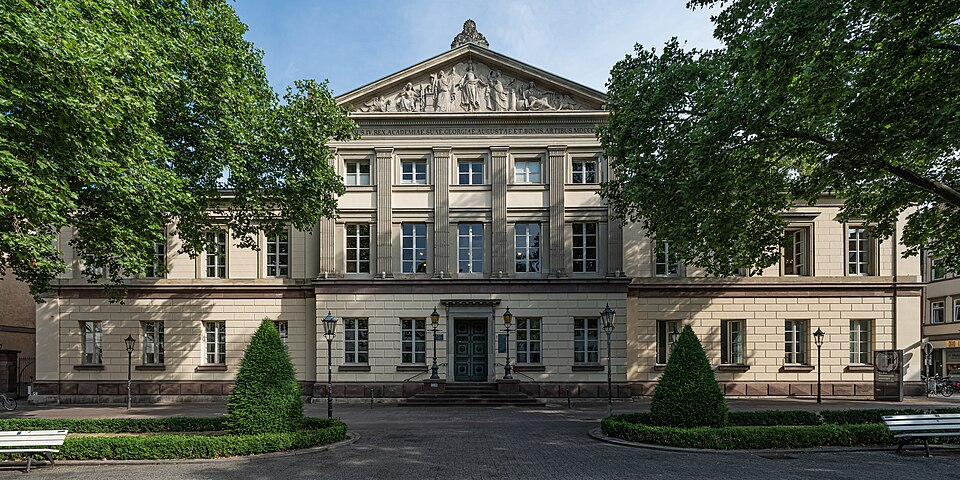
\includegraphics[width=\linewidth]{image/univgottingen.jpg}
			\caption{哥廷根大学（Georg-August-Universität Göttingen）一角，A.Savin 摄}
			\label{fig:univgottingen}
		\end{figure}
		这句话后来被刻在了他在哥廷根的墓碑上——在那座城市，还长眠着我们在序里提到的玻恩。
		
		然而历史开了一个玩笑。就在希尔伯特演讲的前一天，在柯尼斯堡同期举行的一场学术会议上，年轻的哥德尔（Gödel）宣布了一个结果：任何足够强大的数学体系里，总存在既无法证明、也无法否证的命题。数学用最严格的方式，证明了自己的边界。
		
		那么，希尔伯特错了吗？我想把这个问题留给你。只是请记得，人类并没有因为知道了边界而停下脚步；恰恰相反，弄清楚 “什么是不可知的”，本身就是一种知道。愿你在离开这本书之后，依然保有追问的勇气。
		
		如果这本书让你对数学产生了哪怕一点点好奇，那么前面还有很多风景值得一看：
		
		\begin{itemize}
			\item \textbf{随机过程}会告诉你，如何描述一个随时间演变、每一步又都带着不确定性的系统。股价的涨跌、排队等候的顾客、在诉讼程序各阶段之间流转的案件，都是这样的系统。其中最基本的一类叫作马尔可夫链：把状态之间的转移概率排成一个矩阵，系统的长期命运就写在这个矩阵的幂里，写在属于特征值 $1$ 的那个特征向量里。
			\item \textbf{图论与网络分析}会告诉你，如何研究由“关系”构成的世界。人际往来、企业之间的交叉持股、判决书之间的相互引用，都是网络，都可以写成一个邻接矩阵。“谁在这张网里最重要”这个问题的答案，往往又是某个特征向量。
			\item \textbf{常微分方程与动力系统}会把你大一、大二所学连在一起。当一个量的变化速度线性地取决于当前的状态时，系统会增长、衰减还是振荡，很大程度上由一个矩阵的特征值决定。经济增长和市场价格调整的许多模型，都建立在这个想法之上。
			\item \textbf{矩阵分析与数据科学}会告诉你，如何把一张庞大而杂乱的表格，拆解成少数几个“主要模式”。它的核心工具正是第十章介绍过的奇异值分解，那里只是一个开端。推荐系统、文本的主题挖掘、图像压缩，背后都是它。
			\item 如果你只是单纯地喜欢上了“从定义出发、一步步推出结论”的那种感觉，那么不妨读一读\textbf{近世代数}。这是一门极具魅力的学科，也是一门极具难度的学科。你会空前地感受到数学的“对称性”的优美所在。
		\end{itemize}
		
		最后，有关我个人的私心：我写这本书，本意是想让你们转变讨厌数学的心态，从而重新唤起你们对于数学的兴趣。现在看来，一本书能改变的东西相当有限。不过我还是由衷期望，即使各位读者最终仍然选择不再深入学习数学，即使你们忘记了这本书里的所有公式，你们也会不再认为数学只是一种令人厌烦的考试负担；如果你们将来再次遇到数学时，愿意先问一句“这究竟在研究什么”，而不是立刻把它关在自己的世界之外，那么我将会感到无比欣慰。
	}
		\vspace{1em}
		\begin{flushright}
			编者
			% 落款（姓名、日期）留空，由编者自行填写
		\end{flushright}
	
	\nocite{*}
	
	\printbibliography[heading=bibintoc, title=\ebibname]
	\appendix
	%% =====================================================================
%% appendix-prelim.tex　附录：预备知识（求和号、数学归纳法、映射、复数）
%% 用法：在 document.tex 的 \appendix 之后 %% =====================================================================
%% appendix-prelim.tex　附录：预备知识（求和号、数学归纳法、映射、复数）
%% 用法：在 document.tex 的 \appendix 之后 %% =====================================================================
%% appendix-prelim.tex　附录：预备知识（求和号、数学归纳法、映射、复数）
%% 用法：在 document.tex 的 \appendix 之后 \input{appendix-prelim}.
%% =====================================================================

\chapter{预备知识}\label{app:prelim}

本附录回顾正文反复使用、但中学课程里未必系统讲过的四样工具和方法. 除第一节外，每节末尾有几道小练习，答案附在本附录最后.

\section{命题与证明}

本书的大部分篇幅是定理及其证明. 高中课程讲过集合、充分条件与必要条件、全称量词与存在量词；本节在此基础上补充读写证明时最常用的几样逻辑工具，其中逆否命题与反证法在正文中出现得尤其频繁.

\subsection{集合记号}

本书用 $\{x\in A\mid P(x)\}$ 表示集合 $A$ 中满足条件 $P(x)$ 的元素全体，读作``$A$ 中使 $P(x)$ 成立的 $x$ 的集合''. 例如齐次方程组的解集写成 $\{\vv x\in\mathbb{F}^n\mid \vv{Ax}=\zero\}$. 竖线左边说明元素``从哪里取''，右边说明``满足什么条件''.

记号 $A\subset B$ 表示 $A$ 的每个元素都属于 $B$，\textbf{允许} $A=B$. 需要强调 $A\ne B$ 时，本书会另外写明，例如``$W$ 是 $V$ 的子空间且 $W\ne V$''. 空集记为 $\varnothing$.

\subsection{命题与逻辑联结词}

能够判断真假的陈述句称为\textbf{命题}\index{ming4ti2@命题}. 由命题 $P,Q$ 可以组成新的命题：
\begin{itemize}
	\item $P$ 且 $Q$：两者都真时为真；
	\item $P$ 或 $Q$：至少一个为真时为真（数学中的``或''不排斥两者同时成立）；
	\item 非 $P$：$P$ 真时为假，$P$ 假时为真；
	\item 若 $P$ 则 $Q$，记为 $P\Rightarrow Q$：只有在 $P$ 真而 $Q$ 假时为假.
\end{itemize}

最后一条需要特别留意. 下表列出了 $P\Rightarrow Q$ 的真假：
\begin{center}
	\begin{tabular}{ccc}
		\toprule
		$P$ & $Q$ & $P\Rightarrow Q$ \\
		\midrule
		真 & 真 & 真 \\
		真 & 假 & 假 \\
		假 & 真 & 真 \\
		假 & 假 & 真 \\
		\bottomrule
	\end{tabular}
\end{center}
条件 $P$ 不成立时，``若 $P$ 则 $Q$''没有作出任何断言，因而不会是假的. 例如``若 $n$ 阶方阵 $\vv A$ 可逆，则 $\det\vv A\ne0$''对不可逆的矩阵不说任何话，它不可能被一个不可逆矩阵推翻. 要推翻一个``若……则……''的命题，必须找到一个条件成立而结论不成立的例子，这样的例子称为\textbf{反例}\index{fan3li4@反例}.

若 $P\Rightarrow Q$ 与 $Q\Rightarrow P$ 都成立，称 $P$ 与 $Q$ \textbf{等价}，记为 $P\Leftrightarrow Q$，读作``$P$ 当且仅当 $Q$''. 用高中的语言说，$P$ 是 $Q$ 的充分必要条件.

\subsection{逆命题、否命题与逆否命题}

对命题``若 $P$ 则 $Q$''，称
\begin{itemize}
	\item ``若 $Q$ 则 $P$''为它的\textbf{逆命题}\index{ni4ming4ti2@逆命题}；
	\item ``若非 $P$ 则非 $Q$''为它的\textbf{否命题}\index{fou3ming4ti2@否命题}；
	\item ``若非 $Q$ 则非 $P$''为它的\textbf{逆否命题}\index{ni4fou3ming4ti2@逆否命题}.
\end{itemize}

\begin{theorem}
	一个命题与它的逆否命题同真同假.
\end{theorem}
\begin{proof}
	``若 $P$ 则 $Q$''为假，当且仅当 $P$ 真而 $Q$ 假. ``若非 $Q$ 则非 $P$''为假，当且仅当非 $Q$ 真而非 $P$ 假，也就是 $Q$ 假而 $P$ 真. 两者在同一种情形下为假，所以同真同假.
\end{proof}

同理，逆命题与否命题互为逆否命题，因而也同真同假. 但原命题与逆命题之间没有这样的关系.

\begin{example}
	第二章证明了：``若向量组的一部分线性相关，则整个向量组线性相关''. 它的逆否命题是：``若整个向量组线性无关，则它的每一部分都线性无关''. 两句话说的是同一件事，证明了一句就等于证明了另一句.
	
	它的逆命题是``若整个向量组线性相关，则它的某一部分……''——这需要小心. 整个组线性相关时，它的``一部分''可能线性无关：$(1,0)^\trans,(0,1)^\trans,(1,1)^\trans$ 线性相关，但其中任意两个都线性无关.
\end{example}

\begin{pitfallbox}
	\begin{enumerate}
		\item \textbf{原命题成立，逆命题未必成立.} ``若 $\vv A=\vv O$，则 $\vv{AB}=\vv O$''成立，而它的逆命题``若 $\vv{AB}=\vv O$，则 $\vv A=\vv O$''不成立（第三章有反例）. 判据之所以写成``当且仅当''，正是因为两个方向都要单独验证.
		\item \textbf{``非 $P$''不一定是``$P$ 的反义词''.} ``所有分量都是零''的否定是``至少有一个分量不是零''，而不是``所有分量都不是零''.
	\end{enumerate}
\end{pitfallbox}

\subsection{量词与命题的否定}

``对一切 $x$，$P(x)$ 成立''与``存在 $x$，使 $P(x)$ 成立''分别称为全称命题与存在命题，``对一切''与``存在''称为\textbf{量词}\index{liang4ci2@量词}. 否定一个命题时，两种量词互相交换，内部的条件再取否定：
\[
\text{非}(\text{对一切 }x,\ P(x))\iff\text{存在 }x,\ \text{非 }P(x);\qquad
\text{非}(\text{存在 }x,\ P(x))\iff\text{对一切 }x,\ \text{非 }P(x).
\]
命题中有多个量词时，从左到右逐个交换，最后否定最里面的条件.

\begin{example}
	向量组 $\vv\alpha_1,\ldots,\vv\alpha_s$ 线性无关的定义可以写成：
	\begin{center}
		\textbf{对一切} $k_1,\ldots,k_s\in\mathbb{F}$，若 $k_1\vv\alpha_1+\cdots+k_s\vv\alpha_s=\zero$，则 $k_1=\cdots=k_s=0$.
	\end{center}
	``若……则……''为假，当且仅当条件成立而结论不成立. 于是它的否定是
	\begin{center}
		\textbf{存在} $k_1,\ldots,k_s\in\mathbb{F}$，使 $k_1\vv\alpha_1+\cdots+k_s\vv\alpha_s=\zero$，\textbf{并且} $k_1,\ldots,k_s$ 不全为零.
	\end{center}
	这正是线性相关的定义. 线性相关与线性无关不是两个独立的概念，而是一个命题和它的否定.
\end{example}

\begin{pitfallbox}
	\textbf{量词的顺序不能随意交换.} ``对每个非零数 $a$，存在 $b$ 使 $ab=1$''是真的：$b$ 可以随 $a$ 变化，取 $b=a^{-1}$. ``存在 $b$，使对每个非零数 $a$ 都有 $ab=1$''是假的：一个固定的 $b$ 不可能同时是所有数的倒数. 两句话只是``存在''与``对每个''调换了位置，意思完全不同. 读定义时，要注意哪个量随着哪个量变化.
\end{pitfallbox}

\subsection{常见的证明方法}

\paragraph*{直接证明.} 从条件出发，每一步都由定义、已证的定理或运算规则得出，最后得到结论. 本书的大部分证明属于这一类.

\paragraph*{证明逆否命题.} 有时``若非 $Q$ 则非 $P$''比原命题更容易证. 由于两者同真同假，证出逆否命题，原命题也就成立了. 正文中``等价地''``逆否形式''等说法，指的就是这种做法.

\paragraph*{反证法.}\index{fan3zheng4fa3@反证法} 假设结论不成立，由此推出矛盾——与已知条件矛盾，与已证的定理矛盾，或者推出一个自相矛盾的命题，从而断定结论成立.

\begin{example}
	证明：$\sqrt2$ 不是有理数.
\end{example}
\begin{proof}
	假设 $\sqrt2=\frac mn$，其中 $m,n$ 是正整数且没有大于 $1$ 的公因数. 两边平方得 $m^2=2n^2$，所以 $m^2$ 是偶数，从而 $m$ 是偶数. 设 $m=2k$，代入得 $n^2=2k^2$，同理 $n$ 也是偶数. 于是 $m,n$ 有公因数 $2$，与假设矛盾.
\end{proof}

反证法与证明逆否命题很接近，区别在于：证明逆否命题时目标是明确的``非 $P$''；用反证法时，矛盾可以出现在任何地方.

\paragraph*{证明``当且仅当''.} 要证 $P\Leftrightarrow Q$，必须分别证明 $P\Rightarrow Q$（必要性）与 $Q\Rightarrow P$（充分性）. 正文常用``反之''或``另一方面''标出第二个方向的开始.

若要证明几个条件 (1)(2)(3) 互相等价，不必两两证明六次. 只需证 (1)$\Rightarrow$(2)$\Rightarrow$(3)$\Rightarrow$(1)，沿着这个循环，从任何一个条件出发都能推到其他任何一个条件. 第三章关于可逆矩阵的几个等价条件就是这样证明的.

\paragraph*{证明两个集合相等.} 要证 $A=B$，通常分别证明 $A\subset B$ 与 $B\subset A$：任取 $x\in A$，证明 $x\in B$；再反过来.

\paragraph*{证明存在性与唯一性.} ``存在唯一的 $x$ 满足 $P(x)$''包含两件事. 存在性：找到（或构造出）一个满足 $P$ 的 $x$. 唯一性：设 $x_1,x_2$ 都满足 $P$，证明 $x_1=x_2$. 第二章零向量唯一、第三章逆矩阵唯一，都是这样证明的. 唯一性的证明不需要知道 $x$ 是什么，只需要用到``满足 $P$''这一点. 唯一性还常被反过来使用：若已知满足 $P$ 的对象唯一，要证某个对象 $y$ 就是它，只需验证 $y$ 满足 $P$，这种方法称为\textbf{同一法}——例如要证 $(\vv{AB})^{-1}=\vv B^{-1}\vv A^{-1}$，只需验证 $\vv B^{-1}\vv A^{-1}$ 与 $\vv{AB}$ 相乘得 $\vv I$.

\subsection{证明中的惯用语}

\begin{itemize}
	\item \textbf{任取}：表示接下来的论证对每一个元素都成立，所以不能对这个元素附加任何额外的假设.
	\item \textbf{不妨设}：几种情形本质上相同，只写其中一种. 例如``不妨设 $a_{11}\ne0$''，意思是：若 $a_{11}=0$，交换行或重新编号后可以化为这种情形. 读到这里时，应当想一想为什么可以``不妨''.
	\item \textbf{只需证}：把要证的结论化为另一个更容易的命题，并且后者能推出前者. 注意方向：是``后者 $\Rightarrow$ 前者''.
	\item \textbf{显然}、\textbf{容易验证}：作者认为这一步不难，但不等于读者可以跳过. 遇到这样的字眼，最好在草稿纸上补全.
	\item \textbf{证毕}：本书用 $\blacksquare$ 标出证明的结束.
\end{itemize}

\subsection{怎样读一个证明}

\begin{enumerate}
	\item \textbf{注意目标.} 读证明之前，先弄清要证明的是什么. 把结论用自己的话复述一遍；若结论是``当且仅当''，分清哪一个方向是必要性、哪一个是充分性；若是几个条件互相等价，看清证明沿着怎样的顺序循环. 读到中途迷失时，回头看一眼目标：当前这一步离它还有多远？
	\item \textbf{厘清条件.} 找出定理的每个条件在证明的哪一步被用到. 一个条件看起来没有用上，要么是漏看了，要么是它确实可以去掉——后者值得想一想有没有反例. 同时，每一步都要问``凭什么''：依据只能是定义、已证的结论或运算规则，说不出依据则说明此处没有读懂.
	\item \textbf{把握动机.} 一个证明中通常只有一两步是关键，其余都是顺理成章的推演. 要找出这关键的一步，并问自己：作者为什么会想到这样做？把证明中的一般对象换成一个具体对象，逐步计算一遍，往往能看清这一步在做什么. 正文中的``思维动机''栏目也会辅助你解决这个问题.
	\item \textbf{独立复现.} 读懂之后合上书，自己把证明写一遍. 不求逐字复述，但求思路完整，依据清晰. 能达到以上要求，才说明真正读懂了；若遇到卡壳，则需继续学习.
\end{enumerate}

\section{求和号与求积号}\label{app:sum}

\subsection{定义与基本规则}

把 $a_1+a_2+\cdots+a_n$ 简写为
\[\sum_{i=1}^n a_i,\]
读作``对 $i$ 从 $1$ 到 $n$ 求 $a_i$ 的和''. $i$ 称为\textbf{求和指标}\index{qiu2he2 zhi3biao1@求和指标}，它只是一个``占位符''，换成别的字母不改变和的值：$\sum_{i=1}^na_i=\sum_{k=1}^na_k$. 约定 $n<1$ 时（例如 $\sum_{i=1}^0a_i$）和为 $0$.

求和号满足下面几条规则，它们都只是加法交换律、结合律和分配律的改写：
\begin{enumerate}
	\item （线性）$\displaystyle\sum_{i=1}^n(ca_i+db_i)=c\sum_{i=1}^na_i+d\sum_{i=1}^nb_i$；特别地，$\displaystyle\sum_{i=1}^nc=nc$.
	\item （拆分）$\displaystyle\sum_{i=1}^na_i=\sum_{i=1}^ma_i+\sum_{i=m+1}^na_i$（$1\le m<n$）.
	\item （平移指标）$\displaystyle\sum_{i=1}^na_i=\sum_{j=0}^{n-1}a_{j+1}$，即令 $j=i-1$.
	\item （倒序）$\displaystyle\sum_{i=1}^na_i=\sum_{i=1}^na_{n+1-i}$.
\end{enumerate}

\begin{pitfallbox}
	$\displaystyle\sum_{i=1}^na_ib_i$ 一般\textbf{不等于} $\displaystyle\Big(\sum_{i=1}^na_i\Big)\Big(\sum_{i=1}^nb_i\Big)$. 例如 $n=2$ 时，右边展开为 $a_1b_1+a_1b_2+a_2b_1+a_2b_2$，多出了两项``交叉项''. 同样，$\Big(\sum a_i\Big)^2\ne\sum a_i^2$.
\end{pitfallbox}

\subsection{双重求和}

矩阵乘法、行列式和二次型都离不开双重求和. 把 $mn$ 个数 $a_{ij}$ 排成一张 $m$ 行 $n$ 列的表，它们的总和可以先按行加、再把各行的和加起来，也可以先按列加：
\[\sum_{i=1}^m\sum_{j=1}^na_{ij}=\sum_{j=1}^n\sum_{i=1}^ma_{ij}.\]
这就是\textbf{交换求和次序}\index{jiao1huan4 qiu2he2 ci4xu4@交换求和次序}. 例如两个和的乘积可以写成双重求和：
\[\Big(\sum_{i=1}^ma_i\Big)\Big(\sum_{j=1}^nb_j\Big)=\sum_{i=1}^m\sum_{j=1}^na_ib_j.\]
注意两个和要用\textbf{不同的}指标，否则会混淆.

当求和范围不是``长方形''时，要小心地写出范围. 例如对 $1\le i<j\le n$ 求和，表示表格对角线以上的部分：
\[\sum_{1\le i<j\le n}a_{ij}=\sum_{i=1}^{n-1}\sum_{j=i+1}^na_{ij}=\sum_{j=2}^n\sum_{i=1}^{j-1}a_{ij}.\]
第十一章的二次型 $\sum_{i,j}a_{ij}x_ix_j=\sum_ia_{ii}x_i^2+2\sum_{i<j}a_{ij}x_ix_j$（$a_{ij}=a_{ji}$），就是把这张表拆成对角线和上下两个三角形.

\begin{example}
	用双重求和证明矩阵乘法的结合律：设 $\vv A,\vv B,\vv C$ 分别为 $m\times n$、$n\times p$、$p\times q$ 矩阵. $(\vv{AB})\vv C$ 的 $(i,l)$ 元为
	\[\sum_{k=1}^p\Big(\sum_{j=1}^na_{ij}b_{jk}\Big)c_{kl}=\sum_{k=1}^p\sum_{j=1}^na_{ij}b_{jk}c_{kl}=\sum_{j=1}^n\sum_{k=1}^pa_{ij}b_{jk}c_{kl}=\sum_{j=1}^na_{ij}\Big(\sum_{k=1}^pb_{jk}c_{kl}\Big),\]
	最后一式恰是 $\vv A(\vv{BC})$ 的 $(i,l)$ 元. 中间一步就是交换求和次序.
\end{example}

\subsection{求积号}

类似地，$\displaystyle\prod_{i=1}^na_i=a_1a_2\cdots a_n$，约定空积为 $1$. 第五章的 Vandermonde 行列式 $\prod_{1\le i<j\le n}(x_j-x_i)$ 就是对所有满足 $i<j$ 的指标对求积. 注意 $\prod(ca_i)=c^n\prod a_i$，而不是 $c\prod a_i$——这正是 $\det(c\vv A)=c^n\det\vv A$ 的来源.

\begin{exercise}\label{exo:prelim-sum}
	\begin{enumerate}
		\item 计算 $\displaystyle\sum_{i=1}^{4}(2i-1)$ 与 $\displaystyle\sum_{i=1}^{3}\sum_{j=1}^{2}ij$.
		\item 设 $\vv A=(a_{ij})$ 为 $n$ 阶方阵. 用求和号写出 $\tr\vv A$，并证明 $\tr(\vv{AB})=\tr(\vv{BA})$.
		\item 证明 $\displaystyle\Big(\sum_{i=1}^na_i\Big)^2=\sum_{i=1}^na_i^2+2\sum_{1\le i<j\le n}a_ia_j$.
	\end{enumerate}
\end{exercise}

\section{数学归纳法}\label{app:induction}

很多结论是关于``一切正整数 $n$''的，例如``$n$ 阶三角矩阵的行列式等于对角元之积''. 我们不可能对每个 $n$ 逐一验证，数学归纳法提供了一种``一次证完''的办法.

\begin{theorem}[数学归纳法]\index{shu4xue2 gui1na4fa3@数学归纳法}
	设 $P(n)$ 是关于正整数 $n$ 的命题. 若
	\begin{enumerate}
		\item （\textbf{奠基}）$P(1)$ 成立；
		\item （\textbf{归纳步骤}）对任意正整数 $k$，由 $P(k)$ 成立可以推出 $P(k+1)$ 成立，
	\end{enumerate}
	则 $P(n)$ 对一切正整数 $n$ 成立.
\end{theorem}

直观上，奠基推倒了第一块多米诺骨牌，归纳步骤保证每一块倒下都会推倒下一块. 归纳步骤中的``$P(k)$ 成立''称为\textbf{归纳假设}\index{gui1na4 jia3she4@归纳假设}. 起点也可以不是 $1$：若要证明 $n\ge n_0$ 时 $P(n)$ 成立，就从 $P(n_0)$ 奠基.

\begin{example}
	证明 $\displaystyle\sum_{i=1}^n i=\frac{n(n+1)}2$.
\end{example}
\begin{proof}
	$n=1$ 时两边都是 $1$. 设 $n=k$ 时成立，则
	\[\sum_{i=1}^{k+1}i=\sum_{i=1}^ki+(k+1)=\frac{k(k+1)}2+(k+1)=\frac{(k+1)(k+2)}2,\]
	即 $n=k+1$ 时成立.
\end{proof}

\paragraph*{第二数学归纳法.} 有时证明 $P(k+1)$ 需要用到不止 $P(k)$，而是前面所有的 $P(1),\ldots,P(k)$. 这时把归纳步骤改为``若 $P(1),\ldots,P(k)$ 都成立，则 $P(k+1)$ 成立''，结论不变. 这种形式称为\textbf{第二数学归纳法}\index{di4er4 shu4xue2 gui1na4fa3@第二数学归纳法}（或强归纳法）. 第七章唯一分解定理的存在性部分就是这样证明的：把 $f$ 分解为两个次数更低的多项式之积后，对\textbf{任意}更低的次数都要用到归纳假设.

\begin{example}
	Fibonacci 数列满足 $F_0=0$，$F_1=1$，$F_{k+1}=F_k+F_{k-1}$. 证明 $F_n<2^n$ 对一切 $n\ge0$ 成立.
\end{example}
\begin{proof}
	$n=0,1$ 时显然. 设 $n\ge2$，且结论对一切小于 $n$ 的非负整数成立，则 $F_n=F_{n-1}+F_{n-2}<2^{n-1}+2^{n-2}<2^{n-1}+2^{n-1}=2^n$.
\end{proof}
这里奠基要验证两个值，因为归纳步骤用到了前两项.

\begin{pitfallbox}
	\begin{enumerate}
		\item \textbf{只有归纳步骤不够.} 命题``$n=n+1$''满足``若 $k=k+1$ 则 $k+1=k+2$''，但它对任何 $n$ 都不成立——缺的是奠基.
		\item \textbf{归纳步骤必须对每个 $k$ 都成立.} 一个著名的错误``证明''说``所有的马都是同一种颜色''：$n$ 匹马中去掉第一匹，剩下 $n-1$ 匹同色；去掉最后一匹，剩下 $n-1$ 匹也同色；两组有公共的马，所以 $n$ 匹都同色. 错在 $n=2$ 时两组没有公共的马，归纳步骤从 $k=1$ 到 $k=2$ 断掉了.
	\end{enumerate}
\end{pitfallbox}

本书中用归纳法的地方很多：简化阶梯形的存在（第一章）、Gram–Schmidt 正交化（第九章）、谱定理（第十章）都是对维数或向量个数归纳. 读这些证明时，请先找出``对什么归纳''与``归纳假设用在了哪里''.

\begin{exercise}\label{exo:prelim-ind}
	\begin{enumerate}
		\item 证明 $\displaystyle\sum_{i=1}^n i^2=\frac{n(n+1)(2n+1)}6$.
		\item 证明：对一切正整数 $n$，$\begin{pmatrix}1&1\\0&1\end{pmatrix}^n=\begin{pmatrix}1&n\\0&1\end{pmatrix}$.
		\item 证明：$n$ 个元素的集合恰有 $2^n$ 个子集.
	\end{enumerate}
\end{exercise}

\section{映射}\label{app:map}

\begin{definition}
	设 $A,B$ 是两个非空集合. 若按某种法则 $f$，对 $A$ 中的\textbf{每一个}元素 $x$，都有 $B$ 中\textbf{唯一}的元素 $y$ 与之对应，则称 $f$ 是从 $A$ 到 $B$ 的一个\textbf{映射}\index{ying4she4@映射}，记为 $f:A\to B$，$x\mapsto y=f(x)$. $A$ 称为\textbf{定义域}，$B$ 称为\textbf{陪域}；$y=f(x)$ 称为 $x$ 的\textbf{像}，$x$ 称为 $y$ 的一个\textbf{原像}. 集合 $f(A)=\{f(x)\mid x\in A\}\subset B$ 称为 $f$ 的\textbf{像集}.
\end{definition}

中学的函数就是 $A,B$ 都是数集的映射. 本书中的映射还有：把向量变成向量（矩阵乘向量）、把多项式变成多项式（求导）、把矩阵变成数（行列式、迹）等等. 两个映射 $f,g:A\to B$ 相等，指对每个 $x\in A$ 都有 $f(x)=g(x)$.

\subsection{单射、满射与双射}

\begin{definition}
	设 $f:A\to B$.
	\begin{itemize}
		\item 若不同的元素有不同的像，即 $f(x_1)=f(x_2)\Rightarrow x_1=x_2$，称 $f$ 为\textbf{单射}\index{dan1she4@单射}；
		\item 若 $B$ 中每个元素都有原像，即 $f(A)=B$，称 $f$ 为\textbf{满射}\index{man3she4@满射}；
		\item 既单又满的映射称为\textbf{双射}\index{shuang1she4@双射}（或一一对应）.
	\end{itemize}
\end{definition}

\begin{example}
	\begin{enumerate}
		\item $f:\mathbb{R}\to\mathbb{R}$，$x\mapsto x^2$ 既不单（$f(1)=f(-1)$）也不满（$-1$ 没有原像）. 把陪域改为 $[0,+\infty)$，它成为满射；再把定义域也改为 $[0,+\infty)$，它成为双射. 可见单、满与否依赖于定义域和陪域.
		\item $\mathbb{R}^3\to\mathbb{R}^2$，$(x,y,z)^\trans\mapsto(x,y)^\trans$（向 $xy$ 平面投影）是满射，不是单射.
		\item 第二章的坐标映射 $V\to\mathbb{F}^n$ 是双射.
	\end{enumerate}
\end{example}

\subsection{复合与逆映射}

设 $f:A\to B$，$g:B\to C$. 映射 $g\circ f:A\to C$，$x\mapsto g(f(x))$ 称为 $f$ 与 $g$ 的\textbf{复合}\index{fu4he2@复合（映射的）}. 注意写在右边的 $f$ 先作用. 复合满足结合律 $h\circ(g\circ f)=(h\circ g)\circ f$，但一般不满足交换律——这正是矩阵乘法不交换的根源（第四章）.

集合 $A$ 上的\textbf{恒等映射} $\mathrm{id}_A:x\mapsto x$ 满足 $f\circ\mathrm{id}_A=f$，$\mathrm{id}_B\circ f=f$.

\begin{theorem}
	$f:A\to B$ 是双射，当且仅当存在 $g:B\to A$ 使 $g\circ f=\mathrm{id}_A$ 且 $f\circ g=\mathrm{id}_B$. 这样的 $g$ 是唯一的，称为 $f$ 的\textbf{逆映射}\index{ni4ying4she4@逆映射}，记为 $f^{-1}$.
\end{theorem}
\begin{proof}
	若 $f$ 是双射，对每个 $y\in B$，由满射它有原像，由单射原像唯一，令 $g(y)$ 为这个原像即可. 反之，若这样的 $g$ 存在：由 $f(x_1)=f(x_2)$ 得 $x_1=g(f(x_1))=g(f(x_2))=x_2$，故 $f$ 单；对任意 $y\in B$，$y=f(g(y))$，故 $f$ 满. 唯一性：若 $g,g'$ 都满足条件，则 $g=g\circ\mathrm{id}_B=g\circ(f\circ g')=(g\circ f)\circ g'=g'$.
\end{proof}

唯一性的证明与第三章``逆矩阵唯一''的证明一字不差——逆矩阵就是可逆线性变换的逆映射在坐标下的样子.

\begin{remark}
	只有一侧的条件是不够的. 例如在全体实数列构成的集合上，``左移''$S(a_1,a_2,\ldots)=(a_2,a_3,\ldots)$ 与``右移''$R(a_1,a_2,\ldots)=(0,a_1,a_2,\ldots)$ 满足 $S\circ R=\mathrm{id}$，但 $R\circ S\ne\mathrm{id}$：$R$ 单而不满，$S$ 满而不单. 第三章推论~\ref{cor:onesided} 说，对\textbf{有限维}空间上的线性映射（方阵），一侧可逆就够了；这依赖于维数，对一般映射不成立.
\end{remark}

\begin{exercise}\label{exo:prelim-map}
	\begin{enumerate}
		\item 判断下列映射是否单射、满射：(1) $\mathbb{Z}\to\mathbb{Z}$，$n\mapsto2n$；(2) $\mathbb{R}\to\mathbb{R}$，$x\mapsto x^3$；(3) $M_2(\mathbb{R})\to\mathbb{R}$，$\vv A\mapsto\det\vv A$.
		\item 证明：若 $f$，$g$ 都是单射（满射），则 $g\circ f$ 也是单射（满射）.
		\item 设 $f:A\to B$，$g:B\to C$. 证明：若 $g\circ f$ 是单射，则 $f$ 是单射；若 $g\circ f$ 是满射，则 $g$ 是满射.
	\end{enumerate}
\end{exercise}

\section{复数}\label{app:complex}

第七章以后，多项式的根、矩阵的特征值常常是复数. 本节回顾正文用到的复数知识，并给出 48 学时方案所需的代数基本定理与 Vieta 定理.

\subsection{代数形式}

形如 $z=a+b\mathrm i$（$a,b\in\mathbb{R}$，$\mathrm i^2=-1$）的数称为复数，$a$ 与 $b$ 分别称为它的实部与虚部. 复数按通常的代数法则相加、相乘，遇到 $\mathrm i^2$ 就换成 $-1$：
\[(a+b\mathrm i)(c+d\mathrm i)=(ac-bd)+(ad+bc)\mathrm i.\]

称 $\bar z=a-b\mathrm i$ 为 $z$ 的\textbf{共轭复数}\index{gong4e4 fu4shu4@共轭复数}，$|z|=\sqrt{a^2+b^2}$ 为 $z$ 的\textbf{模}\index{mo2@模（复数的）}. 它们满足
\[z\bar z=|z|^2,\qquad \overline{z+w}=\bar z+\bar w,\qquad \overline{zw}=\bar z\,\bar w,\qquad |zw|=|z|\,|w|.\]
$z$ 是实数当且仅当 $z=\bar z$. 除法靠共轭``有理化''：$z\ne0$ 时，$\dfrac1z=\dfrac{\bar z}{|z|^2}$.

\subsection{复平面与三角形式}

把 $z=a+b\mathrm i$ 对应于平面上的点 $(a,b)$，平面就成了\textbf{复平面}\index{fu4ping2mian4@复平面}；第二章说明了这种对应是 $\mathbb{R}$ 上的同构 $\mathbb{C}\cong\mathbb{R}^2$. 用极坐标写 $a=r\cos\theta$，$b=r\sin\theta$，得到\textbf{三角形式}
\[z=r(\cos\theta+\mathrm i\sin\theta),\]
其中 $r=|z|$. 对 $z\ne0$，满足上式的 $\theta$ 称为 $z$ 的一个\textbf{辐角}\index{fu2jiao3@辐角}. 由于正弦、余弦以 $2\pi$ 为周期，$z$ 的辐角有无穷多个，彼此相差 $2\pi$ 的整数倍，它们的全体记为 $\operatorname{Arg}z$. 其中落在 $(-\pi,\pi]$ 内的那一个是唯一的，称为辐角的\textbf{主值}\index{fu2jiao3 zhu3zhi2@辐角主值}，记为 $\arg z$. 于是
\[\operatorname{Arg}z=\{\arg z+2k\pi\mid k\in\mathbb{Z}\}.\]
例如 $\arg\mathrm i=\frac\pi2$，$\arg(-1)=\pi$，$\arg(1-\mathrm i)=-\frac\pi4$，而 $\operatorname{Arg}(-1)=\{\pi+2k\pi\mid k\in\mathbb{Z}\}$. 零的模为 $0$，但它的辐角没有定义.

由两角和公式，
\[r_1(\cos\theta_1+\mathrm i\sin\theta_1)\cdot r_2(\cos\theta_2+\mathrm i\sin\theta_2)=r_1r_2\big(\cos(\theta_1+\theta_2)+\mathrm i\sin(\theta_1+\theta_2)\big),\]
即\textbf{乘法使模相乘、辐角相加}：若 $\theta_1\in\operatorname{Arg}z_1$，$\theta_2\in\operatorname{Arg}z_2$，则 $\theta_1+\theta_2\in\operatorname{Arg}(z_1z_2)$.

\begin{pitfallbox}
	``辐角相加''说的是辐角的\textbf{全体}，对主值不一定成立. 取 $z_1=z_2=-1$，则 $\arg z_1+\arg z_2=2\pi$，而 $\arg(z_1z_2)=\arg1=0$. 两者相差 $2\pi$，正好落在同一个 $\operatorname{Arg}$ 中. 一般地，$\arg(z_1z_2)$ 与 $\arg z_1+\arg z_2$ 相差 $2\pi$ 的某个整数倍（$0$ 或 $\pm2\pi$）.
\end{pitfallbox}

本书采用记号
\[\mathrm e^{\mathrm i\theta}=\cos\theta+\mathrm i\sin\theta\qquad\text{（Euler 公式）}.\]
在本书中可以把它只当作一个记号. 它的合理性在于，上面的乘法规则恰好写成``指数相加''：$\mathrm e^{\mathrm i\alpha}\mathrm e^{\mathrm i\beta}=\mathrm e^{\mathrm i(\alpha+\beta)}$，从而 $(\mathrm e^{\mathrm i\theta})^n=\mathrm e^{\mathrm in\theta}$（De Moivre 公式）.

\subsection{单位根}

方程 $z^n=1$ 的复根称为 $n$ 次\textbf{单位根}\index{dan1wei4gen1@单位根}. 由 De Moivre 公式，它们恰为
\[\omega_k=\mathrm e^{2k\pi\mathrm i/n}\qquad(k=0,1,\ldots,n-1),\]
是单位圆上把圆周 $n$ 等分的 $n$ 个点. 最常用的是 $n=3$：记 $\omega=\mathrm e^{2\pi\mathrm i/3}=-\frac12+\frac{\sqrt3}2\mathrm i$，则
\[\omega^3=1,\qquad 1+\omega+\omega^2=0,\qquad \bar\omega=\omega^2.\]
第二式来自立方差的因式分解且 $\omega\ne1$. 单位根在循环结构中有重要作用. 同样的方法可以对任意非零复数开方：若 $w=\rho(\cos\varphi+\mathrm i\sin\varphi)\ne0$，则
\[\omega=\sqrt[k]{\rho}\Big(\cos\frac\varphi k+\mathrm i\sin\frac\varphi k\Big)\]
满足 $\omega^k=w$. 所以\textbf{每个非零复数都有 $k$ 次方根}（事实上恰有 $k$ 个）. 在实数范围内，负数没有平方根；在复数范围内，这个障碍消失了.

\subsection{代数基本定理与根与系数的关系}

\begin{theorem}[代数基本定理]
	每个次数 $n\ge1$ 的复系数多项式都至少有一个复根. 因此它恰好有 $n$ 个复根（重根按重数计），即可以写成
	\[f(x)=a_n(x-\lambda_1)(x-\lambda_2)\cdots(x-\lambda_n).\]
\end{theorem}

下面的证明只用到高等数学中的一个结论：\textbf{有界闭区域上的连续函数能取到最小值}. 证明的想法是：$|f(z)|$ 一定在某处取到最小值；而只要 $f(z_0)\ne0$，在 $z_0$ 附近总能找到使 $|f|$ 更小的点. 所以最小值只能是 $0$.

\begin{proof}
	设 $f(z)=a_nz^n+\cdots+a_1z+a_0$，$a_n\ne0$，$n\ge1$.
	
	\textbf{第一步：$|f|$ 能取到最小值.} 对 $|z|\ge1$，由三角不等式，
	\[|f(z)|\ge|a_n||z|^n-\sum_{k<n}|a_k||z|^k\ge|z|^n\Big(|a_n|-\frac{1}{|z|}\sum_{k<n}|a_k|\Big).\]
	取 $R\ge1$ 充分大，使 $\frac1R\sum_{k<n}|a_k|\le\frac12|a_n|$ 且 $\frac12|a_n|R^n\ge|a_0|$. 则当 $|z|\ge R$ 时，$|f(z)|\ge\frac12|a_n||z|^n\ge|a_0|=|f(0)|$.
	
	把 $z=x+\mathrm iy$ 看作平面上的点 $(x,y)$，$|f(z)|$ 是 $x,y$ 的连续函数（它是一个关于 $x,y$ 的多项式的算术平方根）. 它在有界闭区域 $\{|z|\le R\}$ 上取到最小值，设在 $z_0$ 处取到. 由于 $0$ 属于这个区域，$|f(z_0)|\le|f(0)|$；而在区域外 $|f(z)|\ge|f(0)|$. 所以 $|f(z_0)|$ 是 $|f|$ 在整个复平面上的最小值.
	
	\textbf{第二步：最小值为零.} 假设 $f(z_0)\ne0$. 把 $f(z_0+h)$ 按 $h$ 的幂展开，得到一个关于 $h$ 的 $n$ 次多项式
	\[f(z_0+h)=b_0+b_kh^k+b_{k+1}h^{k+1}+\cdots+b_nh^n,\]
	其中 $b_0=f(z_0)\ne0$，$b_k$ 是 $b_0$ 之后第一个不为零的系数（由于 $b_n=a_n\ne0$，这样的 $k$ 存在，且 $1\le k\le n$）. 取复数 $\omega$ 使 $\omega^k=-\dfrac{b_0}{b_k}$（每个非零复数都有 $k$ 次方根），再令 $h=t\omega$，其中 $0<t<1$ 是实数. 则 $b_kh^k=-b_0t^k$，于是
	\[f(z_0+t\omega)=b_0(1-t^k)+\sum_{j=k+1}^nb_j\omega^jt^j.\]
	记 $M=\sum_{j>k}|b_j||\omega|^j$. 由于 $0<t<1$ 时 $t^j\le t^{k+1}$，
	\[|f(z_0+t\omega)|\le|b_0|(1-t^k)+Mt^{k+1}=|b_0|-t^k\big(|b_0|-Mt\big).\]
	取 $t$ 足够小，使 $Mt<|b_0|$，右边就严格小于 $|b_0|=|f(z_0)|$. 这与 $|f(z_0)|$ 是最小值矛盾. 故 $f(z_0)=0$.
	
	\textbf{第三步：分解为一次因式.} 由多项式的带余除法，$f(x)=(x-z_0)g(x)+r$，其中 $r$ 是常数. 代入 $x=z_0$ 得 $r=f(z_0)=0$，所以 $f(x)=(x-z_0)g(x)$，$g$ 的次数为 $n-1$，首项系数仍为 $a_n$. 若 $n-1\ge1$，对 $g$ 重复上述论证；如此进行 $n$ 次，即得所述的分解.
\end{proof}

第二步的想法要归功于达朗贝尔：在 $f(z_0)\ne0$ 的点附近，沿着适当选取的方向 $\omega$ 前进一小步，$f$ 的值就会``向原点靠近''. 方向 $\omega$ 的存在，依赖于复数可以开任意次方——这正是实数做不到、复数做得到的地方. 第一步依赖实数的完备性（有界闭区域上的连续函数有最小值）. 第七章的历史回响提到，代数基本定理至今没有只用代数的证明，原因就在这里.

\begin{theorem}[Vieta 定理 / 韦达定理]
	若首一多项式 $x^n+a_{n-1}x^{n-1}+\cdots+a_1x+a_0$ 的 $n$ 个复根为 $\lambda_1,\ldots,\lambda_n$，则
	\[\lambda_1+\lambda_2+\cdots+\lambda_n=-a_{n-1},\qquad\lambda_1\lambda_2\cdots\lambda_n=(-1)^na_0.\]
	一般地，从 $n$ 个根中任取 $k$ 个相乘、再对一切取法求和，等于 $(-1)^ka_{n-k}$.
\end{theorem}

$n=2$ 时就是中学的二次方程情形. 这个定理在第八章会派上用场.

最后，若 $f$ 的系数都是\textbf{实数}且 $f(\lambda)=0$，对 $\sum a_k\lambda^k=0$ 两边取共轭，由 $\bar a_k=a_k$ 得 $f(\bar\lambda)=0$. 所以\textbf{实系数多项式的非实根成对共轭出现}. 实矩阵的特征多项式是实系数的，它的非实特征值因此也成对出现.

\begin{exercise}\label{exo:prelim-complex}
	\begin{enumerate}
		\item 计算 $(1+2\mathrm i)(3-\mathrm i)$，$\dfrac1{1+\mathrm i}$，$|3+4\mathrm i|$.
		\item 把 $1+\mathrm i$ 与 $-1$ 写成三角形式，并计算 $(1+\mathrm i)^8$.
		\item 不解方程，求 $x^3-3x^2+x+5$ 的三个根之和、两两乘积之和与三根之积.
	\end{enumerate}
\end{exercise}

\section*{本附录练习答案}
\addcontentsline{toc}{section}{本附录练习答案}

\paragraph*{练习~\ref{exo:prelim-sum}.} 1. $16$；$\sum_i\sum_jij=(1+2+3)(1+2)=18$. 2. $\tr\vv A=\sum_ia_{ii}$；$\tr(\vv{AB})=\sum_i\sum_ka_{ik}b_{ki}$，交换求和次序并交换字母即为 $\sum_k\sum_ib_{ki}a_{ik}=\tr(\vv{BA})$. 3. 把 $\big(\sum a_i\big)^2=\sum_i\sum_ja_ia_j$ 的表格拆成对角线（$i=j$）与上、下两个三角形，两个三角形之和相等.

\paragraph*{练习~\ref{exo:prelim-ind}.} 1. 归纳步骤：$\frac{k(k+1)(2k+1)}6+(k+1)^2=\frac{(k+1)(k+2)(2k+3)}6$. 2. $\begin{pmatrix}1&k\\0&1\end{pmatrix}\begin{pmatrix}1&1\\0&1\end{pmatrix}=\begin{pmatrix}1&k+1\\0&1\end{pmatrix}$. 3. 加入第 $k+1$ 个元素后，每个旧子集分别``不含''与``含''新元素，子集个数翻倍.

\paragraph*{练习~\ref{exo:prelim-map}.} 1. (1) 单而不满；(2) 双射；(3) 满而不单（$\diag(t,1)$ 取遍一切实数；$\vv O$ 与 $\diag(1,0)$ 的像都是 $0$）. 2. 单射：$g(f(x_1))=g(f(x_2))\Rightarrow f(x_1)=f(x_2)\Rightarrow x_1=x_2$；满射：$z=g(y)$，$y=f(x)$. 3. 若 $f(x_1)=f(x_2)$，则 $g(f(x_1))=g(f(x_2))$，由 $g\circ f$ 单得 $x_1=x_2$；任意 $z\in C$ 有 $z=g(f(x))$，即 $z$ 是 $g$ 在 $f(x)$ 处的值.


\paragraph*{练习~\ref{exo:prelim-complex}.} 1. $5+5\mathrm i$；$\frac12-\frac12\mathrm i$；$5$. 2. $1+\mathrm i=\sqrt2\,\mathrm e^{\mathrm i\pi/4}$，$-1=\mathrm e^{\mathrm i\pi}$；$(1+\mathrm i)^8=(\sqrt2)^8\mathrm e^{2\pi\mathrm i}=16$. 3. 根之和为 $3$，两两乘积之和为 $1$，三根之积为 $-5$.
.
%% =====================================================================

\chapter{预备知识}\label{app:prelim}

本附录回顾正文反复使用、但中学课程里未必系统讲过的四样工具和方法. 除第一节外，每节末尾有几道小练习，答案附在本附录最后.

\section{命题与证明}

本书的大部分篇幅是定理及其证明. 高中课程讲过集合、充分条件与必要条件、全称量词与存在量词；本节在此基础上补充读写证明时最常用的几样逻辑工具，其中逆否命题与反证法在正文中出现得尤其频繁.

\subsection{集合记号}

本书用 $\{x\in A\mid P(x)\}$ 表示集合 $A$ 中满足条件 $P(x)$ 的元素全体，读作``$A$ 中使 $P(x)$ 成立的 $x$ 的集合''. 例如齐次方程组的解集写成 $\{\vv x\in\mathbb{F}^n\mid \vv{Ax}=\zero\}$. 竖线左边说明元素``从哪里取''，右边说明``满足什么条件''.

记号 $A\subset B$ 表示 $A$ 的每个元素都属于 $B$，\textbf{允许} $A=B$. 需要强调 $A\ne B$ 时，本书会另外写明，例如``$W$ 是 $V$ 的子空间且 $W\ne V$''. 空集记为 $\varnothing$.

\subsection{命题与逻辑联结词}

能够判断真假的陈述句称为\textbf{命题}\index{ming4ti2@命题}. 由命题 $P,Q$ 可以组成新的命题：
\begin{itemize}
	\item $P$ 且 $Q$：两者都真时为真；
	\item $P$ 或 $Q$：至少一个为真时为真（数学中的``或''不排斥两者同时成立）；
	\item 非 $P$：$P$ 真时为假，$P$ 假时为真；
	\item 若 $P$ 则 $Q$，记为 $P\Rightarrow Q$：只有在 $P$ 真而 $Q$ 假时为假.
\end{itemize}

最后一条需要特别留意. 下表列出了 $P\Rightarrow Q$ 的真假：
\begin{center}
	\begin{tabular}{ccc}
		\toprule
		$P$ & $Q$ & $P\Rightarrow Q$ \\
		\midrule
		真 & 真 & 真 \\
		真 & 假 & 假 \\
		假 & 真 & 真 \\
		假 & 假 & 真 \\
		\bottomrule
	\end{tabular}
\end{center}
条件 $P$ 不成立时，``若 $P$ 则 $Q$''没有作出任何断言，因而不会是假的. 例如``若 $n$ 阶方阵 $\vv A$ 可逆，则 $\det\vv A\ne0$''对不可逆的矩阵不说任何话，它不可能被一个不可逆矩阵推翻. 要推翻一个``若……则……''的命题，必须找到一个条件成立而结论不成立的例子，这样的例子称为\textbf{反例}\index{fan3li4@反例}.

若 $P\Rightarrow Q$ 与 $Q\Rightarrow P$ 都成立，称 $P$ 与 $Q$ \textbf{等价}，记为 $P\Leftrightarrow Q$，读作``$P$ 当且仅当 $Q$''. 用高中的语言说，$P$ 是 $Q$ 的充分必要条件.

\subsection{逆命题、否命题与逆否命题}

对命题``若 $P$ 则 $Q$''，称
\begin{itemize}
	\item ``若 $Q$ 则 $P$''为它的\textbf{逆命题}\index{ni4ming4ti2@逆命题}；
	\item ``若非 $P$ 则非 $Q$''为它的\textbf{否命题}\index{fou3ming4ti2@否命题}；
	\item ``若非 $Q$ 则非 $P$''为它的\textbf{逆否命题}\index{ni4fou3ming4ti2@逆否命题}.
\end{itemize}

\begin{theorem}
	一个命题与它的逆否命题同真同假.
\end{theorem}
\begin{proof}
	``若 $P$ 则 $Q$''为假，当且仅当 $P$ 真而 $Q$ 假. ``若非 $Q$ 则非 $P$''为假，当且仅当非 $Q$ 真而非 $P$ 假，也就是 $Q$ 假而 $P$ 真. 两者在同一种情形下为假，所以同真同假.
\end{proof}

同理，逆命题与否命题互为逆否命题，因而也同真同假. 但原命题与逆命题之间没有这样的关系.

\begin{example}
	第二章证明了：``若向量组的一部分线性相关，则整个向量组线性相关''. 它的逆否命题是：``若整个向量组线性无关，则它的每一部分都线性无关''. 两句话说的是同一件事，证明了一句就等于证明了另一句.
	
	它的逆命题是``若整个向量组线性相关，则它的某一部分……''——这需要小心. 整个组线性相关时，它的``一部分''可能线性无关：$(1,0)^\trans,(0,1)^\trans,(1,1)^\trans$ 线性相关，但其中任意两个都线性无关.
\end{example}

\begin{pitfallbox}
	\begin{enumerate}
		\item \textbf{原命题成立，逆命题未必成立.} ``若 $\vv A=\vv O$，则 $\vv{AB}=\vv O$''成立，而它的逆命题``若 $\vv{AB}=\vv O$，则 $\vv A=\vv O$''不成立（第三章有反例）. 判据之所以写成``当且仅当''，正是因为两个方向都要单独验证.
		\item \textbf{``非 $P$''不一定是``$P$ 的反义词''.} ``所有分量都是零''的否定是``至少有一个分量不是零''，而不是``所有分量都不是零''.
	\end{enumerate}
\end{pitfallbox}

\subsection{量词与命题的否定}

``对一切 $x$，$P(x)$ 成立''与``存在 $x$，使 $P(x)$ 成立''分别称为全称命题与存在命题，``对一切''与``存在''称为\textbf{量词}\index{liang4ci2@量词}. 否定一个命题时，两种量词互相交换，内部的条件再取否定：
\[
\text{非}(\text{对一切 }x,\ P(x))\iff\text{存在 }x,\ \text{非 }P(x);\qquad
\text{非}(\text{存在 }x,\ P(x))\iff\text{对一切 }x,\ \text{非 }P(x).
\]
命题中有多个量词时，从左到右逐个交换，最后否定最里面的条件.

\begin{example}
	向量组 $\vv\alpha_1,\ldots,\vv\alpha_s$ 线性无关的定义可以写成：
	\begin{center}
		\textbf{对一切} $k_1,\ldots,k_s\in\mathbb{F}$，若 $k_1\vv\alpha_1+\cdots+k_s\vv\alpha_s=\zero$，则 $k_1=\cdots=k_s=0$.
	\end{center}
	``若……则……''为假，当且仅当条件成立而结论不成立. 于是它的否定是
	\begin{center}
		\textbf{存在} $k_1,\ldots,k_s\in\mathbb{F}$，使 $k_1\vv\alpha_1+\cdots+k_s\vv\alpha_s=\zero$，\textbf{并且} $k_1,\ldots,k_s$ 不全为零.
	\end{center}
	这正是线性相关的定义. 线性相关与线性无关不是两个独立的概念，而是一个命题和它的否定.
\end{example}

\begin{pitfallbox}
	\textbf{量词的顺序不能随意交换.} ``对每个非零数 $a$，存在 $b$ 使 $ab=1$''是真的：$b$ 可以随 $a$ 变化，取 $b=a^{-1}$. ``存在 $b$，使对每个非零数 $a$ 都有 $ab=1$''是假的：一个固定的 $b$ 不可能同时是所有数的倒数. 两句话只是``存在''与``对每个''调换了位置，意思完全不同. 读定义时，要注意哪个量随着哪个量变化.
\end{pitfallbox}

\subsection{常见的证明方法}

\paragraph*{直接证明.} 从条件出发，每一步都由定义、已证的定理或运算规则得出，最后得到结论. 本书的大部分证明属于这一类.

\paragraph*{证明逆否命题.} 有时``若非 $Q$ 则非 $P$''比原命题更容易证. 由于两者同真同假，证出逆否命题，原命题也就成立了. 正文中``等价地''``逆否形式''等说法，指的就是这种做法.

\paragraph*{反证法.}\index{fan3zheng4fa3@反证法} 假设结论不成立，由此推出矛盾——与已知条件矛盾，与已证的定理矛盾，或者推出一个自相矛盾的命题，从而断定结论成立.

\begin{example}
	证明：$\sqrt2$ 不是有理数.
\end{example}
\begin{proof}
	假设 $\sqrt2=\frac mn$，其中 $m,n$ 是正整数且没有大于 $1$ 的公因数. 两边平方得 $m^2=2n^2$，所以 $m^2$ 是偶数，从而 $m$ 是偶数. 设 $m=2k$，代入得 $n^2=2k^2$，同理 $n$ 也是偶数. 于是 $m,n$ 有公因数 $2$，与假设矛盾.
\end{proof}

反证法与证明逆否命题很接近，区别在于：证明逆否命题时目标是明确的``非 $P$''；用反证法时，矛盾可以出现在任何地方.

\paragraph*{证明``当且仅当''.} 要证 $P\Leftrightarrow Q$，必须分别证明 $P\Rightarrow Q$（必要性）与 $Q\Rightarrow P$（充分性）. 正文常用``反之''或``另一方面''标出第二个方向的开始.

若要证明几个条件 (1)(2)(3) 互相等价，不必两两证明六次. 只需证 (1)$\Rightarrow$(2)$\Rightarrow$(3)$\Rightarrow$(1)，沿着这个循环，从任何一个条件出发都能推到其他任何一个条件. 第三章关于可逆矩阵的几个等价条件就是这样证明的.

\paragraph*{证明两个集合相等.} 要证 $A=B$，通常分别证明 $A\subset B$ 与 $B\subset A$：任取 $x\in A$，证明 $x\in B$；再反过来.

\paragraph*{证明存在性与唯一性.} ``存在唯一的 $x$ 满足 $P(x)$''包含两件事. 存在性：找到（或构造出）一个满足 $P$ 的 $x$. 唯一性：设 $x_1,x_2$ 都满足 $P$，证明 $x_1=x_2$. 第二章零向量唯一、第三章逆矩阵唯一，都是这样证明的. 唯一性的证明不需要知道 $x$ 是什么，只需要用到``满足 $P$''这一点. 唯一性还常被反过来使用：若已知满足 $P$ 的对象唯一，要证某个对象 $y$ 就是它，只需验证 $y$ 满足 $P$，这种方法称为\textbf{同一法}——例如要证 $(\vv{AB})^{-1}=\vv B^{-1}\vv A^{-1}$，只需验证 $\vv B^{-1}\vv A^{-1}$ 与 $\vv{AB}$ 相乘得 $\vv I$.

\subsection{证明中的惯用语}

\begin{itemize}
	\item \textbf{任取}：表示接下来的论证对每一个元素都成立，所以不能对这个元素附加任何额外的假设.
	\item \textbf{不妨设}：几种情形本质上相同，只写其中一种. 例如``不妨设 $a_{11}\ne0$''，意思是：若 $a_{11}=0$，交换行或重新编号后可以化为这种情形. 读到这里时，应当想一想为什么可以``不妨''.
	\item \textbf{只需证}：把要证的结论化为另一个更容易的命题，并且后者能推出前者. 注意方向：是``后者 $\Rightarrow$ 前者''.
	\item \textbf{显然}、\textbf{容易验证}：作者认为这一步不难，但不等于读者可以跳过. 遇到这样的字眼，最好在草稿纸上补全.
	\item \textbf{证毕}：本书用 $\blacksquare$ 标出证明的结束.
\end{itemize}

\subsection{怎样读一个证明}

\begin{enumerate}
	\item \textbf{注意目标.} 读证明之前，先弄清要证明的是什么. 把结论用自己的话复述一遍；若结论是``当且仅当''，分清哪一个方向是必要性、哪一个是充分性；若是几个条件互相等价，看清证明沿着怎样的顺序循环. 读到中途迷失时，回头看一眼目标：当前这一步离它还有多远？
	\item \textbf{厘清条件.} 找出定理的每个条件在证明的哪一步被用到. 一个条件看起来没有用上，要么是漏看了，要么是它确实可以去掉——后者值得想一想有没有反例. 同时，每一步都要问``凭什么''：依据只能是定义、已证的结论或运算规则，说不出依据则说明此处没有读懂.
	\item \textbf{把握动机.} 一个证明中通常只有一两步是关键，其余都是顺理成章的推演. 要找出这关键的一步，并问自己：作者为什么会想到这样做？把证明中的一般对象换成一个具体对象，逐步计算一遍，往往能看清这一步在做什么. 正文中的``思维动机''栏目也会辅助你解决这个问题.
	\item \textbf{独立复现.} 读懂之后合上书，自己把证明写一遍. 不求逐字复述，但求思路完整，依据清晰. 能达到以上要求，才说明真正读懂了；若遇到卡壳，则需继续学习.
\end{enumerate}

\section{求和号与求积号}\label{app:sum}

\subsection{定义与基本规则}

把 $a_1+a_2+\cdots+a_n$ 简写为
\[\sum_{i=1}^n a_i,\]
读作``对 $i$ 从 $1$ 到 $n$ 求 $a_i$ 的和''. $i$ 称为\textbf{求和指标}\index{qiu2he2 zhi3biao1@求和指标}，它只是一个``占位符''，换成别的字母不改变和的值：$\sum_{i=1}^na_i=\sum_{k=1}^na_k$. 约定 $n<1$ 时（例如 $\sum_{i=1}^0a_i$）和为 $0$.

求和号满足下面几条规则，它们都只是加法交换律、结合律和分配律的改写：
\begin{enumerate}
	\item （线性）$\displaystyle\sum_{i=1}^n(ca_i+db_i)=c\sum_{i=1}^na_i+d\sum_{i=1}^nb_i$；特别地，$\displaystyle\sum_{i=1}^nc=nc$.
	\item （拆分）$\displaystyle\sum_{i=1}^na_i=\sum_{i=1}^ma_i+\sum_{i=m+1}^na_i$（$1\le m<n$）.
	\item （平移指标）$\displaystyle\sum_{i=1}^na_i=\sum_{j=0}^{n-1}a_{j+1}$，即令 $j=i-1$.
	\item （倒序）$\displaystyle\sum_{i=1}^na_i=\sum_{i=1}^na_{n+1-i}$.
\end{enumerate}

\begin{pitfallbox}
	$\displaystyle\sum_{i=1}^na_ib_i$ 一般\textbf{不等于} $\displaystyle\Big(\sum_{i=1}^na_i\Big)\Big(\sum_{i=1}^nb_i\Big)$. 例如 $n=2$ 时，右边展开为 $a_1b_1+a_1b_2+a_2b_1+a_2b_2$，多出了两项``交叉项''. 同样，$\Big(\sum a_i\Big)^2\ne\sum a_i^2$.
\end{pitfallbox}

\subsection{双重求和}

矩阵乘法、行列式和二次型都离不开双重求和. 把 $mn$ 个数 $a_{ij}$ 排成一张 $m$ 行 $n$ 列的表，它们的总和可以先按行加、再把各行的和加起来，也可以先按列加：
\[\sum_{i=1}^m\sum_{j=1}^na_{ij}=\sum_{j=1}^n\sum_{i=1}^ma_{ij}.\]
这就是\textbf{交换求和次序}\index{jiao1huan4 qiu2he2 ci4xu4@交换求和次序}. 例如两个和的乘积可以写成双重求和：
\[\Big(\sum_{i=1}^ma_i\Big)\Big(\sum_{j=1}^nb_j\Big)=\sum_{i=1}^m\sum_{j=1}^na_ib_j.\]
注意两个和要用\textbf{不同的}指标，否则会混淆.

当求和范围不是``长方形''时，要小心地写出范围. 例如对 $1\le i<j\le n$ 求和，表示表格对角线以上的部分：
\[\sum_{1\le i<j\le n}a_{ij}=\sum_{i=1}^{n-1}\sum_{j=i+1}^na_{ij}=\sum_{j=2}^n\sum_{i=1}^{j-1}a_{ij}.\]
第十一章的二次型 $\sum_{i,j}a_{ij}x_ix_j=\sum_ia_{ii}x_i^2+2\sum_{i<j}a_{ij}x_ix_j$（$a_{ij}=a_{ji}$），就是把这张表拆成对角线和上下两个三角形.

\begin{example}
	用双重求和证明矩阵乘法的结合律：设 $\vv A,\vv B,\vv C$ 分别为 $m\times n$、$n\times p$、$p\times q$ 矩阵. $(\vv{AB})\vv C$ 的 $(i,l)$ 元为
	\[\sum_{k=1}^p\Big(\sum_{j=1}^na_{ij}b_{jk}\Big)c_{kl}=\sum_{k=1}^p\sum_{j=1}^na_{ij}b_{jk}c_{kl}=\sum_{j=1}^n\sum_{k=1}^pa_{ij}b_{jk}c_{kl}=\sum_{j=1}^na_{ij}\Big(\sum_{k=1}^pb_{jk}c_{kl}\Big),\]
	最后一式恰是 $\vv A(\vv{BC})$ 的 $(i,l)$ 元. 中间一步就是交换求和次序.
\end{example}

\subsection{求积号}

类似地，$\displaystyle\prod_{i=1}^na_i=a_1a_2\cdots a_n$，约定空积为 $1$. 第五章的 Vandermonde 行列式 $\prod_{1\le i<j\le n}(x_j-x_i)$ 就是对所有满足 $i<j$ 的指标对求积. 注意 $\prod(ca_i)=c^n\prod a_i$，而不是 $c\prod a_i$——这正是 $\det(c\vv A)=c^n\det\vv A$ 的来源.

\begin{exercise}\label{exo:prelim-sum}
	\begin{enumerate}
		\item 计算 $\displaystyle\sum_{i=1}^{4}(2i-1)$ 与 $\displaystyle\sum_{i=1}^{3}\sum_{j=1}^{2}ij$.
		\item 设 $\vv A=(a_{ij})$ 为 $n$ 阶方阵. 用求和号写出 $\tr\vv A$，并证明 $\tr(\vv{AB})=\tr(\vv{BA})$.
		\item 证明 $\displaystyle\Big(\sum_{i=1}^na_i\Big)^2=\sum_{i=1}^na_i^2+2\sum_{1\le i<j\le n}a_ia_j$.
	\end{enumerate}
\end{exercise}

\section{数学归纳法}\label{app:induction}

很多结论是关于``一切正整数 $n$''的，例如``$n$ 阶三角矩阵的行列式等于对角元之积''. 我们不可能对每个 $n$ 逐一验证，数学归纳法提供了一种``一次证完''的办法.

\begin{theorem}[数学归纳法]\index{shu4xue2 gui1na4fa3@数学归纳法}
	设 $P(n)$ 是关于正整数 $n$ 的命题. 若
	\begin{enumerate}
		\item （\textbf{奠基}）$P(1)$ 成立；
		\item （\textbf{归纳步骤}）对任意正整数 $k$，由 $P(k)$ 成立可以推出 $P(k+1)$ 成立，
	\end{enumerate}
	则 $P(n)$ 对一切正整数 $n$ 成立.
\end{theorem}

直观上，奠基推倒了第一块多米诺骨牌，归纳步骤保证每一块倒下都会推倒下一块. 归纳步骤中的``$P(k)$ 成立''称为\textbf{归纳假设}\index{gui1na4 jia3she4@归纳假设}. 起点也可以不是 $1$：若要证明 $n\ge n_0$ 时 $P(n)$ 成立，就从 $P(n_0)$ 奠基.

\begin{example}
	证明 $\displaystyle\sum_{i=1}^n i=\frac{n(n+1)}2$.
\end{example}
\begin{proof}
	$n=1$ 时两边都是 $1$. 设 $n=k$ 时成立，则
	\[\sum_{i=1}^{k+1}i=\sum_{i=1}^ki+(k+1)=\frac{k(k+1)}2+(k+1)=\frac{(k+1)(k+2)}2,\]
	即 $n=k+1$ 时成立.
\end{proof}

\paragraph*{第二数学归纳法.} 有时证明 $P(k+1)$ 需要用到不止 $P(k)$，而是前面所有的 $P(1),\ldots,P(k)$. 这时把归纳步骤改为``若 $P(1),\ldots,P(k)$ 都成立，则 $P(k+1)$ 成立''，结论不变. 这种形式称为\textbf{第二数学归纳法}\index{di4er4 shu4xue2 gui1na4fa3@第二数学归纳法}（或强归纳法）. 第七章唯一分解定理的存在性部分就是这样证明的：把 $f$ 分解为两个次数更低的多项式之积后，对\textbf{任意}更低的次数都要用到归纳假设.

\begin{example}
	Fibonacci 数列满足 $F_0=0$，$F_1=1$，$F_{k+1}=F_k+F_{k-1}$. 证明 $F_n<2^n$ 对一切 $n\ge0$ 成立.
\end{example}
\begin{proof}
	$n=0,1$ 时显然. 设 $n\ge2$，且结论对一切小于 $n$ 的非负整数成立，则 $F_n=F_{n-1}+F_{n-2}<2^{n-1}+2^{n-2}<2^{n-1}+2^{n-1}=2^n$.
\end{proof}
这里奠基要验证两个值，因为归纳步骤用到了前两项.

\begin{pitfallbox}
	\begin{enumerate}
		\item \textbf{只有归纳步骤不够.} 命题``$n=n+1$''满足``若 $k=k+1$ 则 $k+1=k+2$''，但它对任何 $n$ 都不成立——缺的是奠基.
		\item \textbf{归纳步骤必须对每个 $k$ 都成立.} 一个著名的错误``证明''说``所有的马都是同一种颜色''：$n$ 匹马中去掉第一匹，剩下 $n-1$ 匹同色；去掉最后一匹，剩下 $n-1$ 匹也同色；两组有公共的马，所以 $n$ 匹都同色. 错在 $n=2$ 时两组没有公共的马，归纳步骤从 $k=1$ 到 $k=2$ 断掉了.
	\end{enumerate}
\end{pitfallbox}

本书中用归纳法的地方很多：简化阶梯形的存在（第一章）、Gram–Schmidt 正交化（第九章）、谱定理（第十章）都是对维数或向量个数归纳. 读这些证明时，请先找出``对什么归纳''与``归纳假设用在了哪里''.

\begin{exercise}\label{exo:prelim-ind}
	\begin{enumerate}
		\item 证明 $\displaystyle\sum_{i=1}^n i^2=\frac{n(n+1)(2n+1)}6$.
		\item 证明：对一切正整数 $n$，$\begin{pmatrix}1&1\\0&1\end{pmatrix}^n=\begin{pmatrix}1&n\\0&1\end{pmatrix}$.
		\item 证明：$n$ 个元素的集合恰有 $2^n$ 个子集.
	\end{enumerate}
\end{exercise}

\section{映射}\label{app:map}

\begin{definition}
	设 $A,B$ 是两个非空集合. 若按某种法则 $f$，对 $A$ 中的\textbf{每一个}元素 $x$，都有 $B$ 中\textbf{唯一}的元素 $y$ 与之对应，则称 $f$ 是从 $A$ 到 $B$ 的一个\textbf{映射}\index{ying4she4@映射}，记为 $f:A\to B$，$x\mapsto y=f(x)$. $A$ 称为\textbf{定义域}，$B$ 称为\textbf{陪域}；$y=f(x)$ 称为 $x$ 的\textbf{像}，$x$ 称为 $y$ 的一个\textbf{原像}. 集合 $f(A)=\{f(x)\mid x\in A\}\subset B$ 称为 $f$ 的\textbf{像集}.
\end{definition}

中学的函数就是 $A,B$ 都是数集的映射. 本书中的映射还有：把向量变成向量（矩阵乘向量）、把多项式变成多项式（求导）、把矩阵变成数（行列式、迹）等等. 两个映射 $f,g:A\to B$ 相等，指对每个 $x\in A$ 都有 $f(x)=g(x)$.

\subsection{单射、满射与双射}

\begin{definition}
	设 $f:A\to B$.
	\begin{itemize}
		\item 若不同的元素有不同的像，即 $f(x_1)=f(x_2)\Rightarrow x_1=x_2$，称 $f$ 为\textbf{单射}\index{dan1she4@单射}；
		\item 若 $B$ 中每个元素都有原像，即 $f(A)=B$，称 $f$ 为\textbf{满射}\index{man3she4@满射}；
		\item 既单又满的映射称为\textbf{双射}\index{shuang1she4@双射}（或一一对应）.
	\end{itemize}
\end{definition}

\begin{example}
	\begin{enumerate}
		\item $f:\mathbb{R}\to\mathbb{R}$，$x\mapsto x^2$ 既不单（$f(1)=f(-1)$）也不满（$-1$ 没有原像）. 把陪域改为 $[0,+\infty)$，它成为满射；再把定义域也改为 $[0,+\infty)$，它成为双射. 可见单、满与否依赖于定义域和陪域.
		\item $\mathbb{R}^3\to\mathbb{R}^2$，$(x,y,z)^\trans\mapsto(x,y)^\trans$（向 $xy$ 平面投影）是满射，不是单射.
		\item 第二章的坐标映射 $V\to\mathbb{F}^n$ 是双射.
	\end{enumerate}
\end{example}

\subsection{复合与逆映射}

设 $f:A\to B$，$g:B\to C$. 映射 $g\circ f:A\to C$，$x\mapsto g(f(x))$ 称为 $f$ 与 $g$ 的\textbf{复合}\index{fu4he2@复合（映射的）}. 注意写在右边的 $f$ 先作用. 复合满足结合律 $h\circ(g\circ f)=(h\circ g)\circ f$，但一般不满足交换律——这正是矩阵乘法不交换的根源（第四章）.

集合 $A$ 上的\textbf{恒等映射} $\mathrm{id}_A:x\mapsto x$ 满足 $f\circ\mathrm{id}_A=f$，$\mathrm{id}_B\circ f=f$.

\begin{theorem}
	$f:A\to B$ 是双射，当且仅当存在 $g:B\to A$ 使 $g\circ f=\mathrm{id}_A$ 且 $f\circ g=\mathrm{id}_B$. 这样的 $g$ 是唯一的，称为 $f$ 的\textbf{逆映射}\index{ni4ying4she4@逆映射}，记为 $f^{-1}$.
\end{theorem}
\begin{proof}
	若 $f$ 是双射，对每个 $y\in B$，由满射它有原像，由单射原像唯一，令 $g(y)$ 为这个原像即可. 反之，若这样的 $g$ 存在：由 $f(x_1)=f(x_2)$ 得 $x_1=g(f(x_1))=g(f(x_2))=x_2$，故 $f$ 单；对任意 $y\in B$，$y=f(g(y))$，故 $f$ 满. 唯一性：若 $g,g'$ 都满足条件，则 $g=g\circ\mathrm{id}_B=g\circ(f\circ g')=(g\circ f)\circ g'=g'$.
\end{proof}

唯一性的证明与第三章``逆矩阵唯一''的证明一字不差——逆矩阵就是可逆线性变换的逆映射在坐标下的样子.

\begin{remark}
	只有一侧的条件是不够的. 例如在全体实数列构成的集合上，``左移''$S(a_1,a_2,\ldots)=(a_2,a_3,\ldots)$ 与``右移''$R(a_1,a_2,\ldots)=(0,a_1,a_2,\ldots)$ 满足 $S\circ R=\mathrm{id}$，但 $R\circ S\ne\mathrm{id}$：$R$ 单而不满，$S$ 满而不单. 第三章推论~\ref{cor:onesided} 说，对\textbf{有限维}空间上的线性映射（方阵），一侧可逆就够了；这依赖于维数，对一般映射不成立.
\end{remark}

\begin{exercise}\label{exo:prelim-map}
	\begin{enumerate}
		\item 判断下列映射是否单射、满射：(1) $\mathbb{Z}\to\mathbb{Z}$，$n\mapsto2n$；(2) $\mathbb{R}\to\mathbb{R}$，$x\mapsto x^3$；(3) $M_2(\mathbb{R})\to\mathbb{R}$，$\vv A\mapsto\det\vv A$.
		\item 证明：若 $f$，$g$ 都是单射（满射），则 $g\circ f$ 也是单射（满射）.
		\item 设 $f:A\to B$，$g:B\to C$. 证明：若 $g\circ f$ 是单射，则 $f$ 是单射；若 $g\circ f$ 是满射，则 $g$ 是满射.
	\end{enumerate}
\end{exercise}

\section{复数}\label{app:complex}

第七章以后，多项式的根、矩阵的特征值常常是复数. 本节回顾正文用到的复数知识，并给出 48 学时方案所需的代数基本定理与 Vieta 定理.

\subsection{代数形式}

形如 $z=a+b\mathrm i$（$a,b\in\mathbb{R}$，$\mathrm i^2=-1$）的数称为复数，$a$ 与 $b$ 分别称为它的实部与虚部. 复数按通常的代数法则相加、相乘，遇到 $\mathrm i^2$ 就换成 $-1$：
\[(a+b\mathrm i)(c+d\mathrm i)=(ac-bd)+(ad+bc)\mathrm i.\]

称 $\bar z=a-b\mathrm i$ 为 $z$ 的\textbf{共轭复数}\index{gong4e4 fu4shu4@共轭复数}，$|z|=\sqrt{a^2+b^2}$ 为 $z$ 的\textbf{模}\index{mo2@模（复数的）}. 它们满足
\[z\bar z=|z|^2,\qquad \overline{z+w}=\bar z+\bar w,\qquad \overline{zw}=\bar z\,\bar w,\qquad |zw|=|z|\,|w|.\]
$z$ 是实数当且仅当 $z=\bar z$. 除法靠共轭``有理化''：$z\ne0$ 时，$\dfrac1z=\dfrac{\bar z}{|z|^2}$.

\subsection{复平面与三角形式}

把 $z=a+b\mathrm i$ 对应于平面上的点 $(a,b)$，平面就成了\textbf{复平面}\index{fu4ping2mian4@复平面}；第二章说明了这种对应是 $\mathbb{R}$ 上的同构 $\mathbb{C}\cong\mathbb{R}^2$. 用极坐标写 $a=r\cos\theta$，$b=r\sin\theta$，得到\textbf{三角形式}
\[z=r(\cos\theta+\mathrm i\sin\theta),\]
其中 $r=|z|$. 对 $z\ne0$，满足上式的 $\theta$ 称为 $z$ 的一个\textbf{辐角}\index{fu2jiao3@辐角}. 由于正弦、余弦以 $2\pi$ 为周期，$z$ 的辐角有无穷多个，彼此相差 $2\pi$ 的整数倍，它们的全体记为 $\operatorname{Arg}z$. 其中落在 $(-\pi,\pi]$ 内的那一个是唯一的，称为辐角的\textbf{主值}\index{fu2jiao3 zhu3zhi2@辐角主值}，记为 $\arg z$. 于是
\[\operatorname{Arg}z=\{\arg z+2k\pi\mid k\in\mathbb{Z}\}.\]
例如 $\arg\mathrm i=\frac\pi2$，$\arg(-1)=\pi$，$\arg(1-\mathrm i)=-\frac\pi4$，而 $\operatorname{Arg}(-1)=\{\pi+2k\pi\mid k\in\mathbb{Z}\}$. 零的模为 $0$，但它的辐角没有定义.

由两角和公式，
\[r_1(\cos\theta_1+\mathrm i\sin\theta_1)\cdot r_2(\cos\theta_2+\mathrm i\sin\theta_2)=r_1r_2\big(\cos(\theta_1+\theta_2)+\mathrm i\sin(\theta_1+\theta_2)\big),\]
即\textbf{乘法使模相乘、辐角相加}：若 $\theta_1\in\operatorname{Arg}z_1$，$\theta_2\in\operatorname{Arg}z_2$，则 $\theta_1+\theta_2\in\operatorname{Arg}(z_1z_2)$.

\begin{pitfallbox}
	``辐角相加''说的是辐角的\textbf{全体}，对主值不一定成立. 取 $z_1=z_2=-1$，则 $\arg z_1+\arg z_2=2\pi$，而 $\arg(z_1z_2)=\arg1=0$. 两者相差 $2\pi$，正好落在同一个 $\operatorname{Arg}$ 中. 一般地，$\arg(z_1z_2)$ 与 $\arg z_1+\arg z_2$ 相差 $2\pi$ 的某个整数倍（$0$ 或 $\pm2\pi$）.
\end{pitfallbox}

本书采用记号
\[\mathrm e^{\mathrm i\theta}=\cos\theta+\mathrm i\sin\theta\qquad\text{（Euler 公式）}.\]
在本书中可以把它只当作一个记号. 它的合理性在于，上面的乘法规则恰好写成``指数相加''：$\mathrm e^{\mathrm i\alpha}\mathrm e^{\mathrm i\beta}=\mathrm e^{\mathrm i(\alpha+\beta)}$，从而 $(\mathrm e^{\mathrm i\theta})^n=\mathrm e^{\mathrm in\theta}$（De Moivre 公式）.

\subsection{单位根}

方程 $z^n=1$ 的复根称为 $n$ 次\textbf{单位根}\index{dan1wei4gen1@单位根}. 由 De Moivre 公式，它们恰为
\[\omega_k=\mathrm e^{2k\pi\mathrm i/n}\qquad(k=0,1,\ldots,n-1),\]
是单位圆上把圆周 $n$ 等分的 $n$ 个点. 最常用的是 $n=3$：记 $\omega=\mathrm e^{2\pi\mathrm i/3}=-\frac12+\frac{\sqrt3}2\mathrm i$，则
\[\omega^3=1,\qquad 1+\omega+\omega^2=0,\qquad \bar\omega=\omega^2.\]
第二式来自立方差的因式分解且 $\omega\ne1$. 单位根在循环结构中有重要作用. 同样的方法可以对任意非零复数开方：若 $w=\rho(\cos\varphi+\mathrm i\sin\varphi)\ne0$，则
\[\omega=\sqrt[k]{\rho}\Big(\cos\frac\varphi k+\mathrm i\sin\frac\varphi k\Big)\]
满足 $\omega^k=w$. 所以\textbf{每个非零复数都有 $k$ 次方根}（事实上恰有 $k$ 个）. 在实数范围内，负数没有平方根；在复数范围内，这个障碍消失了.

\subsection{代数基本定理与根与系数的关系}

\begin{theorem}[代数基本定理]
	每个次数 $n\ge1$ 的复系数多项式都至少有一个复根. 因此它恰好有 $n$ 个复根（重根按重数计），即可以写成
	\[f(x)=a_n(x-\lambda_1)(x-\lambda_2)\cdots(x-\lambda_n).\]
\end{theorem}

下面的证明只用到高等数学中的一个结论：\textbf{有界闭区域上的连续函数能取到最小值}. 证明的想法是：$|f(z)|$ 一定在某处取到最小值；而只要 $f(z_0)\ne0$，在 $z_0$ 附近总能找到使 $|f|$ 更小的点. 所以最小值只能是 $0$.

\begin{proof}
	设 $f(z)=a_nz^n+\cdots+a_1z+a_0$，$a_n\ne0$，$n\ge1$.
	
	\textbf{第一步：$|f|$ 能取到最小值.} 对 $|z|\ge1$，由三角不等式，
	\[|f(z)|\ge|a_n||z|^n-\sum_{k<n}|a_k||z|^k\ge|z|^n\Big(|a_n|-\frac{1}{|z|}\sum_{k<n}|a_k|\Big).\]
	取 $R\ge1$ 充分大，使 $\frac1R\sum_{k<n}|a_k|\le\frac12|a_n|$ 且 $\frac12|a_n|R^n\ge|a_0|$. 则当 $|z|\ge R$ 时，$|f(z)|\ge\frac12|a_n||z|^n\ge|a_0|=|f(0)|$.
	
	把 $z=x+\mathrm iy$ 看作平面上的点 $(x,y)$，$|f(z)|$ 是 $x,y$ 的连续函数（它是一个关于 $x,y$ 的多项式的算术平方根）. 它在有界闭区域 $\{|z|\le R\}$ 上取到最小值，设在 $z_0$ 处取到. 由于 $0$ 属于这个区域，$|f(z_0)|\le|f(0)|$；而在区域外 $|f(z)|\ge|f(0)|$. 所以 $|f(z_0)|$ 是 $|f|$ 在整个复平面上的最小值.
	
	\textbf{第二步：最小值为零.} 假设 $f(z_0)\ne0$. 把 $f(z_0+h)$ 按 $h$ 的幂展开，得到一个关于 $h$ 的 $n$ 次多项式
	\[f(z_0+h)=b_0+b_kh^k+b_{k+1}h^{k+1}+\cdots+b_nh^n,\]
	其中 $b_0=f(z_0)\ne0$，$b_k$ 是 $b_0$ 之后第一个不为零的系数（由于 $b_n=a_n\ne0$，这样的 $k$ 存在，且 $1\le k\le n$）. 取复数 $\omega$ 使 $\omega^k=-\dfrac{b_0}{b_k}$（每个非零复数都有 $k$ 次方根），再令 $h=t\omega$，其中 $0<t<1$ 是实数. 则 $b_kh^k=-b_0t^k$，于是
	\[f(z_0+t\omega)=b_0(1-t^k)+\sum_{j=k+1}^nb_j\omega^jt^j.\]
	记 $M=\sum_{j>k}|b_j||\omega|^j$. 由于 $0<t<1$ 时 $t^j\le t^{k+1}$，
	\[|f(z_0+t\omega)|\le|b_0|(1-t^k)+Mt^{k+1}=|b_0|-t^k\big(|b_0|-Mt\big).\]
	取 $t$ 足够小，使 $Mt<|b_0|$，右边就严格小于 $|b_0|=|f(z_0)|$. 这与 $|f(z_0)|$ 是最小值矛盾. 故 $f(z_0)=0$.
	
	\textbf{第三步：分解为一次因式.} 由多项式的带余除法，$f(x)=(x-z_0)g(x)+r$，其中 $r$ 是常数. 代入 $x=z_0$ 得 $r=f(z_0)=0$，所以 $f(x)=(x-z_0)g(x)$，$g$ 的次数为 $n-1$，首项系数仍为 $a_n$. 若 $n-1\ge1$，对 $g$ 重复上述论证；如此进行 $n$ 次，即得所述的分解.
\end{proof}

第二步的想法要归功于达朗贝尔：在 $f(z_0)\ne0$ 的点附近，沿着适当选取的方向 $\omega$ 前进一小步，$f$ 的值就会``向原点靠近''. 方向 $\omega$ 的存在，依赖于复数可以开任意次方——这正是实数做不到、复数做得到的地方. 第一步依赖实数的完备性（有界闭区域上的连续函数有最小值）. 第七章的历史回响提到，代数基本定理至今没有只用代数的证明，原因就在这里.

\begin{theorem}[Vieta 定理 / 韦达定理]
	若首一多项式 $x^n+a_{n-1}x^{n-1}+\cdots+a_1x+a_0$ 的 $n$ 个复根为 $\lambda_1,\ldots,\lambda_n$，则
	\[\lambda_1+\lambda_2+\cdots+\lambda_n=-a_{n-1},\qquad\lambda_1\lambda_2\cdots\lambda_n=(-1)^na_0.\]
	一般地，从 $n$ 个根中任取 $k$ 个相乘、再对一切取法求和，等于 $(-1)^ka_{n-k}$.
\end{theorem}

$n=2$ 时就是中学的二次方程情形. 这个定理在第八章会派上用场.

最后，若 $f$ 的系数都是\textbf{实数}且 $f(\lambda)=0$，对 $\sum a_k\lambda^k=0$ 两边取共轭，由 $\bar a_k=a_k$ 得 $f(\bar\lambda)=0$. 所以\textbf{实系数多项式的非实根成对共轭出现}. 实矩阵的特征多项式是实系数的，它的非实特征值因此也成对出现.

\begin{exercise}\label{exo:prelim-complex}
	\begin{enumerate}
		\item 计算 $(1+2\mathrm i)(3-\mathrm i)$，$\dfrac1{1+\mathrm i}$，$|3+4\mathrm i|$.
		\item 把 $1+\mathrm i$ 与 $-1$ 写成三角形式，并计算 $(1+\mathrm i)^8$.
		\item 不解方程，求 $x^3-3x^2+x+5$ 的三个根之和、两两乘积之和与三根之积.
	\end{enumerate}
\end{exercise}

\section*{本附录练习答案}
\addcontentsline{toc}{section}{本附录练习答案}

\paragraph*{练习~\ref{exo:prelim-sum}.} 1. $16$；$\sum_i\sum_jij=(1+2+3)(1+2)=18$. 2. $\tr\vv A=\sum_ia_{ii}$；$\tr(\vv{AB})=\sum_i\sum_ka_{ik}b_{ki}$，交换求和次序并交换字母即为 $\sum_k\sum_ib_{ki}a_{ik}=\tr(\vv{BA})$. 3. 把 $\big(\sum a_i\big)^2=\sum_i\sum_ja_ia_j$ 的表格拆成对角线（$i=j$）与上、下两个三角形，两个三角形之和相等.

\paragraph*{练习~\ref{exo:prelim-ind}.} 1. 归纳步骤：$\frac{k(k+1)(2k+1)}6+(k+1)^2=\frac{(k+1)(k+2)(2k+3)}6$. 2. $\begin{pmatrix}1&k\\0&1\end{pmatrix}\begin{pmatrix}1&1\\0&1\end{pmatrix}=\begin{pmatrix}1&k+1\\0&1\end{pmatrix}$. 3. 加入第 $k+1$ 个元素后，每个旧子集分别``不含''与``含''新元素，子集个数翻倍.

\paragraph*{练习~\ref{exo:prelim-map}.} 1. (1) 单而不满；(2) 双射；(3) 满而不单（$\diag(t,1)$ 取遍一切实数；$\vv O$ 与 $\diag(1,0)$ 的像都是 $0$）. 2. 单射：$g(f(x_1))=g(f(x_2))\Rightarrow f(x_1)=f(x_2)\Rightarrow x_1=x_2$；满射：$z=g(y)$，$y=f(x)$. 3. 若 $f(x_1)=f(x_2)$，则 $g(f(x_1))=g(f(x_2))$，由 $g\circ f$ 单得 $x_1=x_2$；任意 $z\in C$ 有 $z=g(f(x))$，即 $z$ 是 $g$ 在 $f(x)$ 处的值.


\paragraph*{练习~\ref{exo:prelim-complex}.} 1. $5+5\mathrm i$；$\frac12-\frac12\mathrm i$；$5$. 2. $1+\mathrm i=\sqrt2\,\mathrm e^{\mathrm i\pi/4}$，$-1=\mathrm e^{\mathrm i\pi}$；$(1+\mathrm i)^8=(\sqrt2)^8\mathrm e^{2\pi\mathrm i}=16$. 3. 根之和为 $3$，两两乘积之和为 $1$，三根之积为 $-5$.
.
%% =====================================================================

\chapter{预备知识}\label{app:prelim}

本附录回顾正文反复使用、但中学课程里未必系统讲过的四样工具和方法. 除第一节外，每节末尾有几道小练习，答案附在本附录最后.

\section{命题与证明}

本书的大部分篇幅是定理及其证明. 高中课程讲过集合、充分条件与必要条件、全称量词与存在量词；本节在此基础上补充读写证明时最常用的几样逻辑工具，其中逆否命题与反证法在正文中出现得尤其频繁.

\subsection{集合记号}

本书用 $\{x\in A\mid P(x)\}$ 表示集合 $A$ 中满足条件 $P(x)$ 的元素全体，读作``$A$ 中使 $P(x)$ 成立的 $x$ 的集合''. 例如齐次方程组的解集写成 $\{\vv x\in\mathbb{F}^n\mid \vv{Ax}=\zero\}$. 竖线左边说明元素``从哪里取''，右边说明``满足什么条件''.

记号 $A\subset B$ 表示 $A$ 的每个元素都属于 $B$，\textbf{允许} $A=B$. 需要强调 $A\ne B$ 时，本书会另外写明，例如``$W$ 是 $V$ 的子空间且 $W\ne V$''. 空集记为 $\varnothing$.

\subsection{命题与逻辑联结词}

能够判断真假的陈述句称为\textbf{命题}\index{ming4ti2@命题}. 由命题 $P,Q$ 可以组成新的命题：
\begin{itemize}
	\item $P$ 且 $Q$：两者都真时为真；
	\item $P$ 或 $Q$：至少一个为真时为真（数学中的``或''不排斥两者同时成立）；
	\item 非 $P$：$P$ 真时为假，$P$ 假时为真；
	\item 若 $P$ 则 $Q$，记为 $P\Rightarrow Q$：只有在 $P$ 真而 $Q$ 假时为假.
\end{itemize}

最后一条需要特别留意. 下表列出了 $P\Rightarrow Q$ 的真假：
\begin{center}
	\begin{tabular}{ccc}
		\toprule
		$P$ & $Q$ & $P\Rightarrow Q$ \\
		\midrule
		真 & 真 & 真 \\
		真 & 假 & 假 \\
		假 & 真 & 真 \\
		假 & 假 & 真 \\
		\bottomrule
	\end{tabular}
\end{center}
条件 $P$ 不成立时，``若 $P$ 则 $Q$''没有作出任何断言，因而不会是假的. 例如``若 $n$ 阶方阵 $\vv A$ 可逆，则 $\det\vv A\ne0$''对不可逆的矩阵不说任何话，它不可能被一个不可逆矩阵推翻. 要推翻一个``若……则……''的命题，必须找到一个条件成立而结论不成立的例子，这样的例子称为\textbf{反例}\index{fan3li4@反例}.

若 $P\Rightarrow Q$ 与 $Q\Rightarrow P$ 都成立，称 $P$ 与 $Q$ \textbf{等价}，记为 $P\Leftrightarrow Q$，读作``$P$ 当且仅当 $Q$''. 用高中的语言说，$P$ 是 $Q$ 的充分必要条件.

\subsection{逆命题、否命题与逆否命题}

对命题``若 $P$ 则 $Q$''，称
\begin{itemize}
	\item ``若 $Q$ 则 $P$''为它的\textbf{逆命题}\index{ni4ming4ti2@逆命题}；
	\item ``若非 $P$ 则非 $Q$''为它的\textbf{否命题}\index{fou3ming4ti2@否命题}；
	\item ``若非 $Q$ 则非 $P$''为它的\textbf{逆否命题}\index{ni4fou3ming4ti2@逆否命题}.
\end{itemize}

\begin{theorem}
	一个命题与它的逆否命题同真同假.
\end{theorem}
\begin{proof}
	``若 $P$ 则 $Q$''为假，当且仅当 $P$ 真而 $Q$ 假. ``若非 $Q$ 则非 $P$''为假，当且仅当非 $Q$ 真而非 $P$ 假，也就是 $Q$ 假而 $P$ 真. 两者在同一种情形下为假，所以同真同假.
\end{proof}

同理，逆命题与否命题互为逆否命题，因而也同真同假. 但原命题与逆命题之间没有这样的关系.

\begin{example}
	第二章证明了：``若向量组的一部分线性相关，则整个向量组线性相关''. 它的逆否命题是：``若整个向量组线性无关，则它的每一部分都线性无关''. 两句话说的是同一件事，证明了一句就等于证明了另一句.
	
	它的逆命题是``若整个向量组线性相关，则它的某一部分……''——这需要小心. 整个组线性相关时，它的``一部分''可能线性无关：$(1,0)^\trans,(0,1)^\trans,(1,1)^\trans$ 线性相关，但其中任意两个都线性无关.
\end{example}

\begin{pitfallbox}
	\begin{enumerate}
		\item \textbf{原命题成立，逆命题未必成立.} ``若 $\vv A=\vv O$，则 $\vv{AB}=\vv O$''成立，而它的逆命题``若 $\vv{AB}=\vv O$，则 $\vv A=\vv O$''不成立（第三章有反例）. 判据之所以写成``当且仅当''，正是因为两个方向都要单独验证.
		\item \textbf{``非 $P$''不一定是``$P$ 的反义词''.} ``所有分量都是零''的否定是``至少有一个分量不是零''，而不是``所有分量都不是零''.
	\end{enumerate}
\end{pitfallbox}

\subsection{量词与命题的否定}

``对一切 $x$，$P(x)$ 成立''与``存在 $x$，使 $P(x)$ 成立''分别称为全称命题与存在命题，``对一切''与``存在''称为\textbf{量词}\index{liang4ci2@量词}. 否定一个命题时，两种量词互相交换，内部的条件再取否定：
\[
\text{非}(\text{对一切 }x,\ P(x))\iff\text{存在 }x,\ \text{非 }P(x);\qquad
\text{非}(\text{存在 }x,\ P(x))\iff\text{对一切 }x,\ \text{非 }P(x).
\]
命题中有多个量词时，从左到右逐个交换，最后否定最里面的条件.

\begin{example}
	向量组 $\vv\alpha_1,\ldots,\vv\alpha_s$ 线性无关的定义可以写成：
	\begin{center}
		\textbf{对一切} $k_1,\ldots,k_s\in\mathbb{F}$，若 $k_1\vv\alpha_1+\cdots+k_s\vv\alpha_s=\zero$，则 $k_1=\cdots=k_s=0$.
	\end{center}
	``若……则……''为假，当且仅当条件成立而结论不成立. 于是它的否定是
	\begin{center}
		\textbf{存在} $k_1,\ldots,k_s\in\mathbb{F}$，使 $k_1\vv\alpha_1+\cdots+k_s\vv\alpha_s=\zero$，\textbf{并且} $k_1,\ldots,k_s$ 不全为零.
	\end{center}
	这正是线性相关的定义. 线性相关与线性无关不是两个独立的概念，而是一个命题和它的否定.
\end{example}

\begin{pitfallbox}
	\textbf{量词的顺序不能随意交换.} ``对每个非零数 $a$，存在 $b$ 使 $ab=1$''是真的：$b$ 可以随 $a$ 变化，取 $b=a^{-1}$. ``存在 $b$，使对每个非零数 $a$ 都有 $ab=1$''是假的：一个固定的 $b$ 不可能同时是所有数的倒数. 两句话只是``存在''与``对每个''调换了位置，意思完全不同. 读定义时，要注意哪个量随着哪个量变化.
\end{pitfallbox}

\subsection{常见的证明方法}

\paragraph*{直接证明.} 从条件出发，每一步都由定义、已证的定理或运算规则得出，最后得到结论. 本书的大部分证明属于这一类.

\paragraph*{证明逆否命题.} 有时``若非 $Q$ 则非 $P$''比原命题更容易证. 由于两者同真同假，证出逆否命题，原命题也就成立了. 正文中``等价地''``逆否形式''等说法，指的就是这种做法.

\paragraph*{反证法.}\index{fan3zheng4fa3@反证法} 假设结论不成立，由此推出矛盾——与已知条件矛盾，与已证的定理矛盾，或者推出一个自相矛盾的命题，从而断定结论成立.

\begin{example}
	证明：$\sqrt2$ 不是有理数.
\end{example}
\begin{proof}
	假设 $\sqrt2=\frac mn$，其中 $m,n$ 是正整数且没有大于 $1$ 的公因数. 两边平方得 $m^2=2n^2$，所以 $m^2$ 是偶数，从而 $m$ 是偶数. 设 $m=2k$，代入得 $n^2=2k^2$，同理 $n$ 也是偶数. 于是 $m,n$ 有公因数 $2$，与假设矛盾.
\end{proof}

反证法与证明逆否命题很接近，区别在于：证明逆否命题时目标是明确的``非 $P$''；用反证法时，矛盾可以出现在任何地方.

\paragraph*{证明``当且仅当''.} 要证 $P\Leftrightarrow Q$，必须分别证明 $P\Rightarrow Q$（必要性）与 $Q\Rightarrow P$（充分性）. 正文常用``反之''或``另一方面''标出第二个方向的开始.

若要证明几个条件 (1)(2)(3) 互相等价，不必两两证明六次. 只需证 (1)$\Rightarrow$(2)$\Rightarrow$(3)$\Rightarrow$(1)，沿着这个循环，从任何一个条件出发都能推到其他任何一个条件. 第三章关于可逆矩阵的几个等价条件就是这样证明的.

\paragraph*{证明两个集合相等.} 要证 $A=B$，通常分别证明 $A\subset B$ 与 $B\subset A$：任取 $x\in A$，证明 $x\in B$；再反过来.

\paragraph*{证明存在性与唯一性.} ``存在唯一的 $x$ 满足 $P(x)$''包含两件事. 存在性：找到（或构造出）一个满足 $P$ 的 $x$. 唯一性：设 $x_1,x_2$ 都满足 $P$，证明 $x_1=x_2$. 第二章零向量唯一、第三章逆矩阵唯一，都是这样证明的. 唯一性的证明不需要知道 $x$ 是什么，只需要用到``满足 $P$''这一点. 唯一性还常被反过来使用：若已知满足 $P$ 的对象唯一，要证某个对象 $y$ 就是它，只需验证 $y$ 满足 $P$，这种方法称为\textbf{同一法}——例如要证 $(\vv{AB})^{-1}=\vv B^{-1}\vv A^{-1}$，只需验证 $\vv B^{-1}\vv A^{-1}$ 与 $\vv{AB}$ 相乘得 $\vv I$.

\subsection{证明中的惯用语}

\begin{itemize}
	\item \textbf{任取}：表示接下来的论证对每一个元素都成立，所以不能对这个元素附加任何额外的假设.
	\item \textbf{不妨设}：几种情形本质上相同，只写其中一种. 例如``不妨设 $a_{11}\ne0$''，意思是：若 $a_{11}=0$，交换行或重新编号后可以化为这种情形. 读到这里时，应当想一想为什么可以``不妨''.
	\item \textbf{只需证}：把要证的结论化为另一个更容易的命题，并且后者能推出前者. 注意方向：是``后者 $\Rightarrow$ 前者''.
	\item \textbf{显然}、\textbf{容易验证}：作者认为这一步不难，但不等于读者可以跳过. 遇到这样的字眼，最好在草稿纸上补全.
	\item \textbf{证毕}：本书用 $\blacksquare$ 标出证明的结束.
\end{itemize}

\subsection{怎样读一个证明}

\begin{enumerate}
	\item \textbf{注意目标.} 读证明之前，先弄清要证明的是什么. 把结论用自己的话复述一遍；若结论是``当且仅当''，分清哪一个方向是必要性、哪一个是充分性；若是几个条件互相等价，看清证明沿着怎样的顺序循环. 读到中途迷失时，回头看一眼目标：当前这一步离它还有多远？
	\item \textbf{厘清条件.} 找出定理的每个条件在证明的哪一步被用到. 一个条件看起来没有用上，要么是漏看了，要么是它确实可以去掉——后者值得想一想有没有反例. 同时，每一步都要问``凭什么''：依据只能是定义、已证的结论或运算规则，说不出依据则说明此处没有读懂.
	\item \textbf{把握动机.} 一个证明中通常只有一两步是关键，其余都是顺理成章的推演. 要找出这关键的一步，并问自己：作者为什么会想到这样做？把证明中的一般对象换成一个具体对象，逐步计算一遍，往往能看清这一步在做什么. 正文中的``思维动机''栏目也会辅助你解决这个问题.
	\item \textbf{独立复现.} 读懂之后合上书，自己把证明写一遍. 不求逐字复述，但求思路完整，依据清晰. 能达到以上要求，才说明真正读懂了；若遇到卡壳，则需继续学习.
\end{enumerate}

\section{求和号与求积号}\label{app:sum}

\subsection{定义与基本规则}

把 $a_1+a_2+\cdots+a_n$ 简写为
\[\sum_{i=1}^n a_i,\]
读作``对 $i$ 从 $1$ 到 $n$ 求 $a_i$ 的和''. $i$ 称为\textbf{求和指标}\index{qiu2he2 zhi3biao1@求和指标}，它只是一个``占位符''，换成别的字母不改变和的值：$\sum_{i=1}^na_i=\sum_{k=1}^na_k$. 约定 $n<1$ 时（例如 $\sum_{i=1}^0a_i$）和为 $0$.

求和号满足下面几条规则，它们都只是加法交换律、结合律和分配律的改写：
\begin{enumerate}
	\item （线性）$\displaystyle\sum_{i=1}^n(ca_i+db_i)=c\sum_{i=1}^na_i+d\sum_{i=1}^nb_i$；特别地，$\displaystyle\sum_{i=1}^nc=nc$.
	\item （拆分）$\displaystyle\sum_{i=1}^na_i=\sum_{i=1}^ma_i+\sum_{i=m+1}^na_i$（$1\le m<n$）.
	\item （平移指标）$\displaystyle\sum_{i=1}^na_i=\sum_{j=0}^{n-1}a_{j+1}$，即令 $j=i-1$.
	\item （倒序）$\displaystyle\sum_{i=1}^na_i=\sum_{i=1}^na_{n+1-i}$.
\end{enumerate}

\begin{pitfallbox}
	$\displaystyle\sum_{i=1}^na_ib_i$ 一般\textbf{不等于} $\displaystyle\Big(\sum_{i=1}^na_i\Big)\Big(\sum_{i=1}^nb_i\Big)$. 例如 $n=2$ 时，右边展开为 $a_1b_1+a_1b_2+a_2b_1+a_2b_2$，多出了两项``交叉项''. 同样，$\Big(\sum a_i\Big)^2\ne\sum a_i^2$.
\end{pitfallbox}

\subsection{双重求和}

矩阵乘法、行列式和二次型都离不开双重求和. 把 $mn$ 个数 $a_{ij}$ 排成一张 $m$ 行 $n$ 列的表，它们的总和可以先按行加、再把各行的和加起来，也可以先按列加：
\[\sum_{i=1}^m\sum_{j=1}^na_{ij}=\sum_{j=1}^n\sum_{i=1}^ma_{ij}.\]
这就是\textbf{交换求和次序}\index{jiao1huan4 qiu2he2 ci4xu4@交换求和次序}. 例如两个和的乘积可以写成双重求和：
\[\Big(\sum_{i=1}^ma_i\Big)\Big(\sum_{j=1}^nb_j\Big)=\sum_{i=1}^m\sum_{j=1}^na_ib_j.\]
注意两个和要用\textbf{不同的}指标，否则会混淆.

当求和范围不是``长方形''时，要小心地写出范围. 例如对 $1\le i<j\le n$ 求和，表示表格对角线以上的部分：
\[\sum_{1\le i<j\le n}a_{ij}=\sum_{i=1}^{n-1}\sum_{j=i+1}^na_{ij}=\sum_{j=2}^n\sum_{i=1}^{j-1}a_{ij}.\]
第十一章的二次型 $\sum_{i,j}a_{ij}x_ix_j=\sum_ia_{ii}x_i^2+2\sum_{i<j}a_{ij}x_ix_j$（$a_{ij}=a_{ji}$），就是把这张表拆成对角线和上下两个三角形.

\begin{example}
	用双重求和证明矩阵乘法的结合律：设 $\vv A,\vv B,\vv C$ 分别为 $m\times n$、$n\times p$、$p\times q$ 矩阵. $(\vv{AB})\vv C$ 的 $(i,l)$ 元为
	\[\sum_{k=1}^p\Big(\sum_{j=1}^na_{ij}b_{jk}\Big)c_{kl}=\sum_{k=1}^p\sum_{j=1}^na_{ij}b_{jk}c_{kl}=\sum_{j=1}^n\sum_{k=1}^pa_{ij}b_{jk}c_{kl}=\sum_{j=1}^na_{ij}\Big(\sum_{k=1}^pb_{jk}c_{kl}\Big),\]
	最后一式恰是 $\vv A(\vv{BC})$ 的 $(i,l)$ 元. 中间一步就是交换求和次序.
\end{example}

\subsection{求积号}

类似地，$\displaystyle\prod_{i=1}^na_i=a_1a_2\cdots a_n$，约定空积为 $1$. 第五章的 Vandermonde 行列式 $\prod_{1\le i<j\le n}(x_j-x_i)$ 就是对所有满足 $i<j$ 的指标对求积. 注意 $\prod(ca_i)=c^n\prod a_i$，而不是 $c\prod a_i$——这正是 $\det(c\vv A)=c^n\det\vv A$ 的来源.

\begin{exercise}\label{exo:prelim-sum}
	\begin{enumerate}
		\item 计算 $\displaystyle\sum_{i=1}^{4}(2i-1)$ 与 $\displaystyle\sum_{i=1}^{3}\sum_{j=1}^{2}ij$.
		\item 设 $\vv A=(a_{ij})$ 为 $n$ 阶方阵. 用求和号写出 $\tr\vv A$，并证明 $\tr(\vv{AB})=\tr(\vv{BA})$.
		\item 证明 $\displaystyle\Big(\sum_{i=1}^na_i\Big)^2=\sum_{i=1}^na_i^2+2\sum_{1\le i<j\le n}a_ia_j$.
	\end{enumerate}
\end{exercise}

\section{数学归纳法}\label{app:induction}

很多结论是关于``一切正整数 $n$''的，例如``$n$ 阶三角矩阵的行列式等于对角元之积''. 我们不可能对每个 $n$ 逐一验证，数学归纳法提供了一种``一次证完''的办法.

\begin{theorem}[数学归纳法]\index{shu4xue2 gui1na4fa3@数学归纳法}
	设 $P(n)$ 是关于正整数 $n$ 的命题. 若
	\begin{enumerate}
		\item （\textbf{奠基}）$P(1)$ 成立；
		\item （\textbf{归纳步骤}）对任意正整数 $k$，由 $P(k)$ 成立可以推出 $P(k+1)$ 成立，
	\end{enumerate}
	则 $P(n)$ 对一切正整数 $n$ 成立.
\end{theorem}

直观上，奠基推倒了第一块多米诺骨牌，归纳步骤保证每一块倒下都会推倒下一块. 归纳步骤中的``$P(k)$ 成立''称为\textbf{归纳假设}\index{gui1na4 jia3she4@归纳假设}. 起点也可以不是 $1$：若要证明 $n\ge n_0$ 时 $P(n)$ 成立，就从 $P(n_0)$ 奠基.

\begin{example}
	证明 $\displaystyle\sum_{i=1}^n i=\frac{n(n+1)}2$.
\end{example}
\begin{proof}
	$n=1$ 时两边都是 $1$. 设 $n=k$ 时成立，则
	\[\sum_{i=1}^{k+1}i=\sum_{i=1}^ki+(k+1)=\frac{k(k+1)}2+(k+1)=\frac{(k+1)(k+2)}2,\]
	即 $n=k+1$ 时成立.
\end{proof}

\paragraph*{第二数学归纳法.} 有时证明 $P(k+1)$ 需要用到不止 $P(k)$，而是前面所有的 $P(1),\ldots,P(k)$. 这时把归纳步骤改为``若 $P(1),\ldots,P(k)$ 都成立，则 $P(k+1)$ 成立''，结论不变. 这种形式称为\textbf{第二数学归纳法}\index{di4er4 shu4xue2 gui1na4fa3@第二数学归纳法}（或强归纳法）. 第七章唯一分解定理的存在性部分就是这样证明的：把 $f$ 分解为两个次数更低的多项式之积后，对\textbf{任意}更低的次数都要用到归纳假设.

\begin{example}
	Fibonacci 数列满足 $F_0=0$，$F_1=1$，$F_{k+1}=F_k+F_{k-1}$. 证明 $F_n<2^n$ 对一切 $n\ge0$ 成立.
\end{example}
\begin{proof}
	$n=0,1$ 时显然. 设 $n\ge2$，且结论对一切小于 $n$ 的非负整数成立，则 $F_n=F_{n-1}+F_{n-2}<2^{n-1}+2^{n-2}<2^{n-1}+2^{n-1}=2^n$.
\end{proof}
这里奠基要验证两个值，因为归纳步骤用到了前两项.

\begin{pitfallbox}
	\begin{enumerate}
		\item \textbf{只有归纳步骤不够.} 命题``$n=n+1$''满足``若 $k=k+1$ 则 $k+1=k+2$''，但它对任何 $n$ 都不成立——缺的是奠基.
		\item \textbf{归纳步骤必须对每个 $k$ 都成立.} 一个著名的错误``证明''说``所有的马都是同一种颜色''：$n$ 匹马中去掉第一匹，剩下 $n-1$ 匹同色；去掉最后一匹，剩下 $n-1$ 匹也同色；两组有公共的马，所以 $n$ 匹都同色. 错在 $n=2$ 时两组没有公共的马，归纳步骤从 $k=1$ 到 $k=2$ 断掉了.
	\end{enumerate}
\end{pitfallbox}

本书中用归纳法的地方很多：简化阶梯形的存在（第一章）、Gram–Schmidt 正交化（第九章）、谱定理（第十章）都是对维数或向量个数归纳. 读这些证明时，请先找出``对什么归纳''与``归纳假设用在了哪里''.

\begin{exercise}\label{exo:prelim-ind}
	\begin{enumerate}
		\item 证明 $\displaystyle\sum_{i=1}^n i^2=\frac{n(n+1)(2n+1)}6$.
		\item 证明：对一切正整数 $n$，$\begin{pmatrix}1&1\\0&1\end{pmatrix}^n=\begin{pmatrix}1&n\\0&1\end{pmatrix}$.
		\item 证明：$n$ 个元素的集合恰有 $2^n$ 个子集.
	\end{enumerate}
\end{exercise}

\section{映射}\label{app:map}

\begin{definition}
	设 $A,B$ 是两个非空集合. 若按某种法则 $f$，对 $A$ 中的\textbf{每一个}元素 $x$，都有 $B$ 中\textbf{唯一}的元素 $y$ 与之对应，则称 $f$ 是从 $A$ 到 $B$ 的一个\textbf{映射}\index{ying4she4@映射}，记为 $f:A\to B$，$x\mapsto y=f(x)$. $A$ 称为\textbf{定义域}，$B$ 称为\textbf{陪域}；$y=f(x)$ 称为 $x$ 的\textbf{像}，$x$ 称为 $y$ 的一个\textbf{原像}. 集合 $f(A)=\{f(x)\mid x\in A\}\subset B$ 称为 $f$ 的\textbf{像集}.
\end{definition}

中学的函数就是 $A,B$ 都是数集的映射. 本书中的映射还有：把向量变成向量（矩阵乘向量）、把多项式变成多项式（求导）、把矩阵变成数（行列式、迹）等等. 两个映射 $f,g:A\to B$ 相等，指对每个 $x\in A$ 都有 $f(x)=g(x)$.

\subsection{单射、满射与双射}

\begin{definition}
	设 $f:A\to B$.
	\begin{itemize}
		\item 若不同的元素有不同的像，即 $f(x_1)=f(x_2)\Rightarrow x_1=x_2$，称 $f$ 为\textbf{单射}\index{dan1she4@单射}；
		\item 若 $B$ 中每个元素都有原像，即 $f(A)=B$，称 $f$ 为\textbf{满射}\index{man3she4@满射}；
		\item 既单又满的映射称为\textbf{双射}\index{shuang1she4@双射}（或一一对应）.
	\end{itemize}
\end{definition}

\begin{example}
	\begin{enumerate}
		\item $f:\mathbb{R}\to\mathbb{R}$，$x\mapsto x^2$ 既不单（$f(1)=f(-1)$）也不满（$-1$ 没有原像）. 把陪域改为 $[0,+\infty)$，它成为满射；再把定义域也改为 $[0,+\infty)$，它成为双射. 可见单、满与否依赖于定义域和陪域.
		\item $\mathbb{R}^3\to\mathbb{R}^2$，$(x,y,z)^\trans\mapsto(x,y)^\trans$（向 $xy$ 平面投影）是满射，不是单射.
		\item 第二章的坐标映射 $V\to\mathbb{F}^n$ 是双射.
	\end{enumerate}
\end{example}

\subsection{复合与逆映射}

设 $f:A\to B$，$g:B\to C$. 映射 $g\circ f:A\to C$，$x\mapsto g(f(x))$ 称为 $f$ 与 $g$ 的\textbf{复合}\index{fu4he2@复合（映射的）}. 注意写在右边的 $f$ 先作用. 复合满足结合律 $h\circ(g\circ f)=(h\circ g)\circ f$，但一般不满足交换律——这正是矩阵乘法不交换的根源（第四章）.

集合 $A$ 上的\textbf{恒等映射} $\mathrm{id}_A:x\mapsto x$ 满足 $f\circ\mathrm{id}_A=f$，$\mathrm{id}_B\circ f=f$.

\begin{theorem}
	$f:A\to B$ 是双射，当且仅当存在 $g:B\to A$ 使 $g\circ f=\mathrm{id}_A$ 且 $f\circ g=\mathrm{id}_B$. 这样的 $g$ 是唯一的，称为 $f$ 的\textbf{逆映射}\index{ni4ying4she4@逆映射}，记为 $f^{-1}$.
\end{theorem}
\begin{proof}
	若 $f$ 是双射，对每个 $y\in B$，由满射它有原像，由单射原像唯一，令 $g(y)$ 为这个原像即可. 反之，若这样的 $g$ 存在：由 $f(x_1)=f(x_2)$ 得 $x_1=g(f(x_1))=g(f(x_2))=x_2$，故 $f$ 单；对任意 $y\in B$，$y=f(g(y))$，故 $f$ 满. 唯一性：若 $g,g'$ 都满足条件，则 $g=g\circ\mathrm{id}_B=g\circ(f\circ g')=(g\circ f)\circ g'=g'$.
\end{proof}

唯一性的证明与第三章``逆矩阵唯一''的证明一字不差——逆矩阵就是可逆线性变换的逆映射在坐标下的样子.

\begin{remark}
	只有一侧的条件是不够的. 例如在全体实数列构成的集合上，``左移''$S(a_1,a_2,\ldots)=(a_2,a_3,\ldots)$ 与``右移''$R(a_1,a_2,\ldots)=(0,a_1,a_2,\ldots)$ 满足 $S\circ R=\mathrm{id}$，但 $R\circ S\ne\mathrm{id}$：$R$ 单而不满，$S$ 满而不单. 第三章推论~\ref{cor:onesided} 说，对\textbf{有限维}空间上的线性映射（方阵），一侧可逆就够了；这依赖于维数，对一般映射不成立.
\end{remark}

\begin{exercise}\label{exo:prelim-map}
	\begin{enumerate}
		\item 判断下列映射是否单射、满射：(1) $\mathbb{Z}\to\mathbb{Z}$，$n\mapsto2n$；(2) $\mathbb{R}\to\mathbb{R}$，$x\mapsto x^3$；(3) $M_2(\mathbb{R})\to\mathbb{R}$，$\vv A\mapsto\det\vv A$.
		\item 证明：若 $f$，$g$ 都是单射（满射），则 $g\circ f$ 也是单射（满射）.
		\item 设 $f:A\to B$，$g:B\to C$. 证明：若 $g\circ f$ 是单射，则 $f$ 是单射；若 $g\circ f$ 是满射，则 $g$ 是满射.
	\end{enumerate}
\end{exercise}

\section{复数}\label{app:complex}

第七章以后，多项式的根、矩阵的特征值常常是复数. 本节回顾正文用到的复数知识，并给出 48 学时方案所需的代数基本定理与 Vieta 定理.

\subsection{代数形式}

形如 $z=a+b\mathrm i$（$a,b\in\mathbb{R}$，$\mathrm i^2=-1$）的数称为复数，$a$ 与 $b$ 分别称为它的实部与虚部. 复数按通常的代数法则相加、相乘，遇到 $\mathrm i^2$ 就换成 $-1$：
\[(a+b\mathrm i)(c+d\mathrm i)=(ac-bd)+(ad+bc)\mathrm i.\]

称 $\bar z=a-b\mathrm i$ 为 $z$ 的\textbf{共轭复数}\index{gong4e4 fu4shu4@共轭复数}，$|z|=\sqrt{a^2+b^2}$ 为 $z$ 的\textbf{模}\index{mo2@模（复数的）}. 它们满足
\[z\bar z=|z|^2,\qquad \overline{z+w}=\bar z+\bar w,\qquad \overline{zw}=\bar z\,\bar w,\qquad |zw|=|z|\,|w|.\]
$z$ 是实数当且仅当 $z=\bar z$. 除法靠共轭``有理化''：$z\ne0$ 时，$\dfrac1z=\dfrac{\bar z}{|z|^2}$.

\subsection{复平面与三角形式}

把 $z=a+b\mathrm i$ 对应于平面上的点 $(a,b)$，平面就成了\textbf{复平面}\index{fu4ping2mian4@复平面}；第二章说明了这种对应是 $\mathbb{R}$ 上的同构 $\mathbb{C}\cong\mathbb{R}^2$. 用极坐标写 $a=r\cos\theta$，$b=r\sin\theta$，得到\textbf{三角形式}
\[z=r(\cos\theta+\mathrm i\sin\theta),\]
其中 $r=|z|$. 对 $z\ne0$，满足上式的 $\theta$ 称为 $z$ 的一个\textbf{辐角}\index{fu2jiao3@辐角}. 由于正弦、余弦以 $2\pi$ 为周期，$z$ 的辐角有无穷多个，彼此相差 $2\pi$ 的整数倍，它们的全体记为 $\operatorname{Arg}z$. 其中落在 $(-\pi,\pi]$ 内的那一个是唯一的，称为辐角的\textbf{主值}\index{fu2jiao3 zhu3zhi2@辐角主值}，记为 $\arg z$. 于是
\[\operatorname{Arg}z=\{\arg z+2k\pi\mid k\in\mathbb{Z}\}.\]
例如 $\arg\mathrm i=\frac\pi2$，$\arg(-1)=\pi$，$\arg(1-\mathrm i)=-\frac\pi4$，而 $\operatorname{Arg}(-1)=\{\pi+2k\pi\mid k\in\mathbb{Z}\}$. 零的模为 $0$，但它的辐角没有定义.

由两角和公式，
\[r_1(\cos\theta_1+\mathrm i\sin\theta_1)\cdot r_2(\cos\theta_2+\mathrm i\sin\theta_2)=r_1r_2\big(\cos(\theta_1+\theta_2)+\mathrm i\sin(\theta_1+\theta_2)\big),\]
即\textbf{乘法使模相乘、辐角相加}：若 $\theta_1\in\operatorname{Arg}z_1$，$\theta_2\in\operatorname{Arg}z_2$，则 $\theta_1+\theta_2\in\operatorname{Arg}(z_1z_2)$.

\begin{pitfallbox}
	``辐角相加''说的是辐角的\textbf{全体}，对主值不一定成立. 取 $z_1=z_2=-1$，则 $\arg z_1+\arg z_2=2\pi$，而 $\arg(z_1z_2)=\arg1=0$. 两者相差 $2\pi$，正好落在同一个 $\operatorname{Arg}$ 中. 一般地，$\arg(z_1z_2)$ 与 $\arg z_1+\arg z_2$ 相差 $2\pi$ 的某个整数倍（$0$ 或 $\pm2\pi$）.
\end{pitfallbox}

本书采用记号
\[\mathrm e^{\mathrm i\theta}=\cos\theta+\mathrm i\sin\theta\qquad\text{（Euler 公式）}.\]
在本书中可以把它只当作一个记号. 它的合理性在于，上面的乘法规则恰好写成``指数相加''：$\mathrm e^{\mathrm i\alpha}\mathrm e^{\mathrm i\beta}=\mathrm e^{\mathrm i(\alpha+\beta)}$，从而 $(\mathrm e^{\mathrm i\theta})^n=\mathrm e^{\mathrm in\theta}$（De Moivre 公式）.

\subsection{单位根}

方程 $z^n=1$ 的复根称为 $n$ 次\textbf{单位根}\index{dan1wei4gen1@单位根}. 由 De Moivre 公式，它们恰为
\[\omega_k=\mathrm e^{2k\pi\mathrm i/n}\qquad(k=0,1,\ldots,n-1),\]
是单位圆上把圆周 $n$ 等分的 $n$ 个点. 最常用的是 $n=3$：记 $\omega=\mathrm e^{2\pi\mathrm i/3}=-\frac12+\frac{\sqrt3}2\mathrm i$，则
\[\omega^3=1,\qquad 1+\omega+\omega^2=0,\qquad \bar\omega=\omega^2.\]
第二式来自立方差的因式分解且 $\omega\ne1$. 单位根在循环结构中有重要作用. 同样的方法可以对任意非零复数开方：若 $w=\rho(\cos\varphi+\mathrm i\sin\varphi)\ne0$，则
\[\omega=\sqrt[k]{\rho}\Big(\cos\frac\varphi k+\mathrm i\sin\frac\varphi k\Big)\]
满足 $\omega^k=w$. 所以\textbf{每个非零复数都有 $k$ 次方根}（事实上恰有 $k$ 个）. 在实数范围内，负数没有平方根；在复数范围内，这个障碍消失了.

\subsection{代数基本定理与根与系数的关系}

\begin{theorem}[代数基本定理]
	每个次数 $n\ge1$ 的复系数多项式都至少有一个复根. 因此它恰好有 $n$ 个复根（重根按重数计），即可以写成
	\[f(x)=a_n(x-\lambda_1)(x-\lambda_2)\cdots(x-\lambda_n).\]
\end{theorem}

下面的证明只用到高等数学中的一个结论：\textbf{有界闭区域上的连续函数能取到最小值}. 证明的想法是：$|f(z)|$ 一定在某处取到最小值；而只要 $f(z_0)\ne0$，在 $z_0$ 附近总能找到使 $|f|$ 更小的点. 所以最小值只能是 $0$.

\begin{proof}
	设 $f(z)=a_nz^n+\cdots+a_1z+a_0$，$a_n\ne0$，$n\ge1$.
	
	\textbf{第一步：$|f|$ 能取到最小值.} 对 $|z|\ge1$，由三角不等式，
	\[|f(z)|\ge|a_n||z|^n-\sum_{k<n}|a_k||z|^k\ge|z|^n\Big(|a_n|-\frac{1}{|z|}\sum_{k<n}|a_k|\Big).\]
	取 $R\ge1$ 充分大，使 $\frac1R\sum_{k<n}|a_k|\le\frac12|a_n|$ 且 $\frac12|a_n|R^n\ge|a_0|$. 则当 $|z|\ge R$ 时，$|f(z)|\ge\frac12|a_n||z|^n\ge|a_0|=|f(0)|$.
	
	把 $z=x+\mathrm iy$ 看作平面上的点 $(x,y)$，$|f(z)|$ 是 $x,y$ 的连续函数（它是一个关于 $x,y$ 的多项式的算术平方根）. 它在有界闭区域 $\{|z|\le R\}$ 上取到最小值，设在 $z_0$ 处取到. 由于 $0$ 属于这个区域，$|f(z_0)|\le|f(0)|$；而在区域外 $|f(z)|\ge|f(0)|$. 所以 $|f(z_0)|$ 是 $|f|$ 在整个复平面上的最小值.
	
	\textbf{第二步：最小值为零.} 假设 $f(z_0)\ne0$. 把 $f(z_0+h)$ 按 $h$ 的幂展开，得到一个关于 $h$ 的 $n$ 次多项式
	\[f(z_0+h)=b_0+b_kh^k+b_{k+1}h^{k+1}+\cdots+b_nh^n,\]
	其中 $b_0=f(z_0)\ne0$，$b_k$ 是 $b_0$ 之后第一个不为零的系数（由于 $b_n=a_n\ne0$，这样的 $k$ 存在，且 $1\le k\le n$）. 取复数 $\omega$ 使 $\omega^k=-\dfrac{b_0}{b_k}$（每个非零复数都有 $k$ 次方根），再令 $h=t\omega$，其中 $0<t<1$ 是实数. 则 $b_kh^k=-b_0t^k$，于是
	\[f(z_0+t\omega)=b_0(1-t^k)+\sum_{j=k+1}^nb_j\omega^jt^j.\]
	记 $M=\sum_{j>k}|b_j||\omega|^j$. 由于 $0<t<1$ 时 $t^j\le t^{k+1}$，
	\[|f(z_0+t\omega)|\le|b_0|(1-t^k)+Mt^{k+1}=|b_0|-t^k\big(|b_0|-Mt\big).\]
	取 $t$ 足够小，使 $Mt<|b_0|$，右边就严格小于 $|b_0|=|f(z_0)|$. 这与 $|f(z_0)|$ 是最小值矛盾. 故 $f(z_0)=0$.
	
	\textbf{第三步：分解为一次因式.} 由多项式的带余除法，$f(x)=(x-z_0)g(x)+r$，其中 $r$ 是常数. 代入 $x=z_0$ 得 $r=f(z_0)=0$，所以 $f(x)=(x-z_0)g(x)$，$g$ 的次数为 $n-1$，首项系数仍为 $a_n$. 若 $n-1\ge1$，对 $g$ 重复上述论证；如此进行 $n$ 次，即得所述的分解.
\end{proof}

第二步的想法要归功于达朗贝尔：在 $f(z_0)\ne0$ 的点附近，沿着适当选取的方向 $\omega$ 前进一小步，$f$ 的值就会``向原点靠近''. 方向 $\omega$ 的存在，依赖于复数可以开任意次方——这正是实数做不到、复数做得到的地方. 第一步依赖实数的完备性（有界闭区域上的连续函数有最小值）. 第七章的历史回响提到，代数基本定理至今没有只用代数的证明，原因就在这里.

\begin{theorem}[Vieta 定理 / 韦达定理]
	若首一多项式 $x^n+a_{n-1}x^{n-1}+\cdots+a_1x+a_0$ 的 $n$ 个复根为 $\lambda_1,\ldots,\lambda_n$，则
	\[\lambda_1+\lambda_2+\cdots+\lambda_n=-a_{n-1},\qquad\lambda_1\lambda_2\cdots\lambda_n=(-1)^na_0.\]
	一般地，从 $n$ 个根中任取 $k$ 个相乘、再对一切取法求和，等于 $(-1)^ka_{n-k}$.
\end{theorem}

$n=2$ 时就是中学的二次方程情形. 这个定理在第八章会派上用场.

最后，若 $f$ 的系数都是\textbf{实数}且 $f(\lambda)=0$，对 $\sum a_k\lambda^k=0$ 两边取共轭，由 $\bar a_k=a_k$ 得 $f(\bar\lambda)=0$. 所以\textbf{实系数多项式的非实根成对共轭出现}. 实矩阵的特征多项式是实系数的，它的非实特征值因此也成对出现.

\begin{exercise}\label{exo:prelim-complex}
	\begin{enumerate}
		\item 计算 $(1+2\mathrm i)(3-\mathrm i)$，$\dfrac1{1+\mathrm i}$，$|3+4\mathrm i|$.
		\item 把 $1+\mathrm i$ 与 $-1$ 写成三角形式，并计算 $(1+\mathrm i)^8$.
		\item 不解方程，求 $x^3-3x^2+x+5$ 的三个根之和、两两乘积之和与三根之积.
	\end{enumerate}
\end{exercise}

\section*{本附录练习答案}
\addcontentsline{toc}{section}{本附录练习答案}

\paragraph*{练习~\ref{exo:prelim-sum}.} 1. $16$；$\sum_i\sum_jij=(1+2+3)(1+2)=18$. 2. $\tr\vv A=\sum_ia_{ii}$；$\tr(\vv{AB})=\sum_i\sum_ka_{ik}b_{ki}$，交换求和次序并交换字母即为 $\sum_k\sum_ib_{ki}a_{ik}=\tr(\vv{BA})$. 3. 把 $\big(\sum a_i\big)^2=\sum_i\sum_ja_ia_j$ 的表格拆成对角线（$i=j$）与上、下两个三角形，两个三角形之和相等.

\paragraph*{练习~\ref{exo:prelim-ind}.} 1. 归纳步骤：$\frac{k(k+1)(2k+1)}6+(k+1)^2=\frac{(k+1)(k+2)(2k+3)}6$. 2. $\begin{pmatrix}1&k\\0&1\end{pmatrix}\begin{pmatrix}1&1\\0&1\end{pmatrix}=\begin{pmatrix}1&k+1\\0&1\end{pmatrix}$. 3. 加入第 $k+1$ 个元素后，每个旧子集分别``不含''与``含''新元素，子集个数翻倍.

\paragraph*{练习~\ref{exo:prelim-map}.} 1. (1) 单而不满；(2) 双射；(3) 满而不单（$\diag(t,1)$ 取遍一切实数；$\vv O$ 与 $\diag(1,0)$ 的像都是 $0$）. 2. 单射：$g(f(x_1))=g(f(x_2))\Rightarrow f(x_1)=f(x_2)\Rightarrow x_1=x_2$；满射：$z=g(y)$，$y=f(x)$. 3. 若 $f(x_1)=f(x_2)$，则 $g(f(x_1))=g(f(x_2))$，由 $g\circ f$ 单得 $x_1=x_2$；任意 $z\in C$ 有 $z=g(f(x))$，即 $z$ 是 $g$ 在 $f(x)$ 处的值.


\paragraph*{练习~\ref{exo:prelim-complex}.} 1. $5+5\mathrm i$；$\frac12-\frac12\mathrm i$；$5$. 2. $1+\mathrm i=\sqrt2\,\mathrm e^{\mathrm i\pi/4}$，$-1=\mathrm e^{\mathrm i\pi}$；$(1+\mathrm i)^8=(\sqrt2)^8\mathrm e^{2\pi\mathrm i}=16$. 3. 根之和为 $3$，两两乘积之和为 $1$，三根之积为 $-5$.
  % 附录 A　预备知识：求和号、数学归纳法、映射
	%% =====================================================================
%% appendix-or.tex　附录：运筹学初步（线性规划）
%% 用法：在 document.tex 中 %% =====================================================================
%% appendix-prelim.tex　附录：预备知识（求和号、数学归纳法、映射、复数）
%% 用法：在 document.tex 的 \appendix 之后 %% =====================================================================
%% appendix-prelim.tex　附录：预备知识（求和号、数学归纳法、映射、复数）
%% 用法：在 document.tex 的 \appendix 之后 \input{appendix-prelim}.
%% =====================================================================

\chapter{预备知识}\label{app:prelim}

本附录回顾正文反复使用、但中学课程里未必系统讲过的四样工具和方法. 除第一节外，每节末尾有几道小练习，答案附在本附录最后.

\section{命题与证明}

本书的大部分篇幅是定理及其证明. 高中课程讲过集合、充分条件与必要条件、全称量词与存在量词；本节在此基础上补充读写证明时最常用的几样逻辑工具，其中逆否命题与反证法在正文中出现得尤其频繁.

\subsection{集合记号}

本书用 $\{x\in A\mid P(x)\}$ 表示集合 $A$ 中满足条件 $P(x)$ 的元素全体，读作``$A$ 中使 $P(x)$ 成立的 $x$ 的集合''. 例如齐次方程组的解集写成 $\{\vv x\in\mathbb{F}^n\mid \vv{Ax}=\zero\}$. 竖线左边说明元素``从哪里取''，右边说明``满足什么条件''.

记号 $A\subset B$ 表示 $A$ 的每个元素都属于 $B$，\textbf{允许} $A=B$. 需要强调 $A\ne B$ 时，本书会另外写明，例如``$W$ 是 $V$ 的子空间且 $W\ne V$''. 空集记为 $\varnothing$.

\subsection{命题与逻辑联结词}

能够判断真假的陈述句称为\textbf{命题}\index{ming4ti2@命题}. 由命题 $P,Q$ 可以组成新的命题：
\begin{itemize}
	\item $P$ 且 $Q$：两者都真时为真；
	\item $P$ 或 $Q$：至少一个为真时为真（数学中的``或''不排斥两者同时成立）；
	\item 非 $P$：$P$ 真时为假，$P$ 假时为真；
	\item 若 $P$ 则 $Q$，记为 $P\Rightarrow Q$：只有在 $P$ 真而 $Q$ 假时为假.
\end{itemize}

最后一条需要特别留意. 下表列出了 $P\Rightarrow Q$ 的真假：
\begin{center}
	\begin{tabular}{ccc}
		\toprule
		$P$ & $Q$ & $P\Rightarrow Q$ \\
		\midrule
		真 & 真 & 真 \\
		真 & 假 & 假 \\
		假 & 真 & 真 \\
		假 & 假 & 真 \\
		\bottomrule
	\end{tabular}
\end{center}
条件 $P$ 不成立时，``若 $P$ 则 $Q$''没有作出任何断言，因而不会是假的. 例如``若 $n$ 阶方阵 $\vv A$ 可逆，则 $\det\vv A\ne0$''对不可逆的矩阵不说任何话，它不可能被一个不可逆矩阵推翻. 要推翻一个``若……则……''的命题，必须找到一个条件成立而结论不成立的例子，这样的例子称为\textbf{反例}\index{fan3li4@反例}.

若 $P\Rightarrow Q$ 与 $Q\Rightarrow P$ 都成立，称 $P$ 与 $Q$ \textbf{等价}，记为 $P\Leftrightarrow Q$，读作``$P$ 当且仅当 $Q$''. 用高中的语言说，$P$ 是 $Q$ 的充分必要条件.

\subsection{逆命题、否命题与逆否命题}

对命题``若 $P$ 则 $Q$''，称
\begin{itemize}
	\item ``若 $Q$ 则 $P$''为它的\textbf{逆命题}\index{ni4ming4ti2@逆命题}；
	\item ``若非 $P$ 则非 $Q$''为它的\textbf{否命题}\index{fou3ming4ti2@否命题}；
	\item ``若非 $Q$ 则非 $P$''为它的\textbf{逆否命题}\index{ni4fou3ming4ti2@逆否命题}.
\end{itemize}

\begin{theorem}
	一个命题与它的逆否命题同真同假.
\end{theorem}
\begin{proof}
	``若 $P$ 则 $Q$''为假，当且仅当 $P$ 真而 $Q$ 假. ``若非 $Q$ 则非 $P$''为假，当且仅当非 $Q$ 真而非 $P$ 假，也就是 $Q$ 假而 $P$ 真. 两者在同一种情形下为假，所以同真同假.
\end{proof}

同理，逆命题与否命题互为逆否命题，因而也同真同假. 但原命题与逆命题之间没有这样的关系.

\begin{example}
	第二章证明了：``若向量组的一部分线性相关，则整个向量组线性相关''. 它的逆否命题是：``若整个向量组线性无关，则它的每一部分都线性无关''. 两句话说的是同一件事，证明了一句就等于证明了另一句.
	
	它的逆命题是``若整个向量组线性相关，则它的某一部分……''——这需要小心. 整个组线性相关时，它的``一部分''可能线性无关：$(1,0)^\trans,(0,1)^\trans,(1,1)^\trans$ 线性相关，但其中任意两个都线性无关.
\end{example}

\begin{pitfallbox}
	\begin{enumerate}
		\item \textbf{原命题成立，逆命题未必成立.} ``若 $\vv A=\vv O$，则 $\vv{AB}=\vv O$''成立，而它的逆命题``若 $\vv{AB}=\vv O$，则 $\vv A=\vv O$''不成立（第三章有反例）. 判据之所以写成``当且仅当''，正是因为两个方向都要单独验证.
		\item \textbf{``非 $P$''不一定是``$P$ 的反义词''.} ``所有分量都是零''的否定是``至少有一个分量不是零''，而不是``所有分量都不是零''.
	\end{enumerate}
\end{pitfallbox}

\subsection{量词与命题的否定}

``对一切 $x$，$P(x)$ 成立''与``存在 $x$，使 $P(x)$ 成立''分别称为全称命题与存在命题，``对一切''与``存在''称为\textbf{量词}\index{liang4ci2@量词}. 否定一个命题时，两种量词互相交换，内部的条件再取否定：
\[
\text{非}(\text{对一切 }x,\ P(x))\iff\text{存在 }x,\ \text{非 }P(x);\qquad
\text{非}(\text{存在 }x,\ P(x))\iff\text{对一切 }x,\ \text{非 }P(x).
\]
命题中有多个量词时，从左到右逐个交换，最后否定最里面的条件.

\begin{example}
	向量组 $\vv\alpha_1,\ldots,\vv\alpha_s$ 线性无关的定义可以写成：
	\begin{center}
		\textbf{对一切} $k_1,\ldots,k_s\in\mathbb{F}$，若 $k_1\vv\alpha_1+\cdots+k_s\vv\alpha_s=\zero$，则 $k_1=\cdots=k_s=0$.
	\end{center}
	``若……则……''为假，当且仅当条件成立而结论不成立. 于是它的否定是
	\begin{center}
		\textbf{存在} $k_1,\ldots,k_s\in\mathbb{F}$，使 $k_1\vv\alpha_1+\cdots+k_s\vv\alpha_s=\zero$，\textbf{并且} $k_1,\ldots,k_s$ 不全为零.
	\end{center}
	这正是线性相关的定义. 线性相关与线性无关不是两个独立的概念，而是一个命题和它的否定.
\end{example}

\begin{pitfallbox}
	\textbf{量词的顺序不能随意交换.} ``对每个非零数 $a$，存在 $b$ 使 $ab=1$''是真的：$b$ 可以随 $a$ 变化，取 $b=a^{-1}$. ``存在 $b$，使对每个非零数 $a$ 都有 $ab=1$''是假的：一个固定的 $b$ 不可能同时是所有数的倒数. 两句话只是``存在''与``对每个''调换了位置，意思完全不同. 读定义时，要注意哪个量随着哪个量变化.
\end{pitfallbox}

\subsection{常见的证明方法}

\paragraph*{直接证明.} 从条件出发，每一步都由定义、已证的定理或运算规则得出，最后得到结论. 本书的大部分证明属于这一类.

\paragraph*{证明逆否命题.} 有时``若非 $Q$ 则非 $P$''比原命题更容易证. 由于两者同真同假，证出逆否命题，原命题也就成立了. 正文中``等价地''``逆否形式''等说法，指的就是这种做法.

\paragraph*{反证法.}\index{fan3zheng4fa3@反证法} 假设结论不成立，由此推出矛盾——与已知条件矛盾，与已证的定理矛盾，或者推出一个自相矛盾的命题，从而断定结论成立.

\begin{example}
	证明：$\sqrt2$ 不是有理数.
\end{example}
\begin{proof}
	假设 $\sqrt2=\frac mn$，其中 $m,n$ 是正整数且没有大于 $1$ 的公因数. 两边平方得 $m^2=2n^2$，所以 $m^2$ 是偶数，从而 $m$ 是偶数. 设 $m=2k$，代入得 $n^2=2k^2$，同理 $n$ 也是偶数. 于是 $m,n$ 有公因数 $2$，与假设矛盾.
\end{proof}

反证法与证明逆否命题很接近，区别在于：证明逆否命题时目标是明确的``非 $P$''；用反证法时，矛盾可以出现在任何地方.

\paragraph*{证明``当且仅当''.} 要证 $P\Leftrightarrow Q$，必须分别证明 $P\Rightarrow Q$（必要性）与 $Q\Rightarrow P$（充分性）. 正文常用``反之''或``另一方面''标出第二个方向的开始.

若要证明几个条件 (1)(2)(3) 互相等价，不必两两证明六次. 只需证 (1)$\Rightarrow$(2)$\Rightarrow$(3)$\Rightarrow$(1)，沿着这个循环，从任何一个条件出发都能推到其他任何一个条件. 第三章关于可逆矩阵的几个等价条件就是这样证明的.

\paragraph*{证明两个集合相等.} 要证 $A=B$，通常分别证明 $A\subset B$ 与 $B\subset A$：任取 $x\in A$，证明 $x\in B$；再反过来.

\paragraph*{证明存在性与唯一性.} ``存在唯一的 $x$ 满足 $P(x)$''包含两件事. 存在性：找到（或构造出）一个满足 $P$ 的 $x$. 唯一性：设 $x_1,x_2$ 都满足 $P$，证明 $x_1=x_2$. 第二章零向量唯一、第三章逆矩阵唯一，都是这样证明的. 唯一性的证明不需要知道 $x$ 是什么，只需要用到``满足 $P$''这一点. 唯一性还常被反过来使用：若已知满足 $P$ 的对象唯一，要证某个对象 $y$ 就是它，只需验证 $y$ 满足 $P$，这种方法称为\textbf{同一法}——例如要证 $(\vv{AB})^{-1}=\vv B^{-1}\vv A^{-1}$，只需验证 $\vv B^{-1}\vv A^{-1}$ 与 $\vv{AB}$ 相乘得 $\vv I$.

\subsection{证明中的惯用语}

\begin{itemize}
	\item \textbf{任取}：表示接下来的论证对每一个元素都成立，所以不能对这个元素附加任何额外的假设.
	\item \textbf{不妨设}：几种情形本质上相同，只写其中一种. 例如``不妨设 $a_{11}\ne0$''，意思是：若 $a_{11}=0$，交换行或重新编号后可以化为这种情形. 读到这里时，应当想一想为什么可以``不妨''.
	\item \textbf{只需证}：把要证的结论化为另一个更容易的命题，并且后者能推出前者. 注意方向：是``后者 $\Rightarrow$ 前者''.
	\item \textbf{显然}、\textbf{容易验证}：作者认为这一步不难，但不等于读者可以跳过. 遇到这样的字眼，最好在草稿纸上补全.
	\item \textbf{证毕}：本书用 $\blacksquare$ 标出证明的结束.
\end{itemize}

\subsection{怎样读一个证明}

\begin{enumerate}
	\item \textbf{注意目标.} 读证明之前，先弄清要证明的是什么. 把结论用自己的话复述一遍；若结论是``当且仅当''，分清哪一个方向是必要性、哪一个是充分性；若是几个条件互相等价，看清证明沿着怎样的顺序循环. 读到中途迷失时，回头看一眼目标：当前这一步离它还有多远？
	\item \textbf{厘清条件.} 找出定理的每个条件在证明的哪一步被用到. 一个条件看起来没有用上，要么是漏看了，要么是它确实可以去掉——后者值得想一想有没有反例. 同时，每一步都要问``凭什么''：依据只能是定义、已证的结论或运算规则，说不出依据则说明此处没有读懂.
	\item \textbf{把握动机.} 一个证明中通常只有一两步是关键，其余都是顺理成章的推演. 要找出这关键的一步，并问自己：作者为什么会想到这样做？把证明中的一般对象换成一个具体对象，逐步计算一遍，往往能看清这一步在做什么. 正文中的``思维动机''栏目也会辅助你解决这个问题.
	\item \textbf{独立复现.} 读懂之后合上书，自己把证明写一遍. 不求逐字复述，但求思路完整，依据清晰. 能达到以上要求，才说明真正读懂了；若遇到卡壳，则需继续学习.
\end{enumerate}

\section{求和号与求积号}\label{app:sum}

\subsection{定义与基本规则}

把 $a_1+a_2+\cdots+a_n$ 简写为
\[\sum_{i=1}^n a_i,\]
读作``对 $i$ 从 $1$ 到 $n$ 求 $a_i$ 的和''. $i$ 称为\textbf{求和指标}\index{qiu2he2 zhi3biao1@求和指标}，它只是一个``占位符''，换成别的字母不改变和的值：$\sum_{i=1}^na_i=\sum_{k=1}^na_k$. 约定 $n<1$ 时（例如 $\sum_{i=1}^0a_i$）和为 $0$.

求和号满足下面几条规则，它们都只是加法交换律、结合律和分配律的改写：
\begin{enumerate}
	\item （线性）$\displaystyle\sum_{i=1}^n(ca_i+db_i)=c\sum_{i=1}^na_i+d\sum_{i=1}^nb_i$；特别地，$\displaystyle\sum_{i=1}^nc=nc$.
	\item （拆分）$\displaystyle\sum_{i=1}^na_i=\sum_{i=1}^ma_i+\sum_{i=m+1}^na_i$（$1\le m<n$）.
	\item （平移指标）$\displaystyle\sum_{i=1}^na_i=\sum_{j=0}^{n-1}a_{j+1}$，即令 $j=i-1$.
	\item （倒序）$\displaystyle\sum_{i=1}^na_i=\sum_{i=1}^na_{n+1-i}$.
\end{enumerate}

\begin{pitfallbox}
	$\displaystyle\sum_{i=1}^na_ib_i$ 一般\textbf{不等于} $\displaystyle\Big(\sum_{i=1}^na_i\Big)\Big(\sum_{i=1}^nb_i\Big)$. 例如 $n=2$ 时，右边展开为 $a_1b_1+a_1b_2+a_2b_1+a_2b_2$，多出了两项``交叉项''. 同样，$\Big(\sum a_i\Big)^2\ne\sum a_i^2$.
\end{pitfallbox}

\subsection{双重求和}

矩阵乘法、行列式和二次型都离不开双重求和. 把 $mn$ 个数 $a_{ij}$ 排成一张 $m$ 行 $n$ 列的表，它们的总和可以先按行加、再把各行的和加起来，也可以先按列加：
\[\sum_{i=1}^m\sum_{j=1}^na_{ij}=\sum_{j=1}^n\sum_{i=1}^ma_{ij}.\]
这就是\textbf{交换求和次序}\index{jiao1huan4 qiu2he2 ci4xu4@交换求和次序}. 例如两个和的乘积可以写成双重求和：
\[\Big(\sum_{i=1}^ma_i\Big)\Big(\sum_{j=1}^nb_j\Big)=\sum_{i=1}^m\sum_{j=1}^na_ib_j.\]
注意两个和要用\textbf{不同的}指标，否则会混淆.

当求和范围不是``长方形''时，要小心地写出范围. 例如对 $1\le i<j\le n$ 求和，表示表格对角线以上的部分：
\[\sum_{1\le i<j\le n}a_{ij}=\sum_{i=1}^{n-1}\sum_{j=i+1}^na_{ij}=\sum_{j=2}^n\sum_{i=1}^{j-1}a_{ij}.\]
第十一章的二次型 $\sum_{i,j}a_{ij}x_ix_j=\sum_ia_{ii}x_i^2+2\sum_{i<j}a_{ij}x_ix_j$（$a_{ij}=a_{ji}$），就是把这张表拆成对角线和上下两个三角形.

\begin{example}
	用双重求和证明矩阵乘法的结合律：设 $\vv A,\vv B,\vv C$ 分别为 $m\times n$、$n\times p$、$p\times q$ 矩阵. $(\vv{AB})\vv C$ 的 $(i,l)$ 元为
	\[\sum_{k=1}^p\Big(\sum_{j=1}^na_{ij}b_{jk}\Big)c_{kl}=\sum_{k=1}^p\sum_{j=1}^na_{ij}b_{jk}c_{kl}=\sum_{j=1}^n\sum_{k=1}^pa_{ij}b_{jk}c_{kl}=\sum_{j=1}^na_{ij}\Big(\sum_{k=1}^pb_{jk}c_{kl}\Big),\]
	最后一式恰是 $\vv A(\vv{BC})$ 的 $(i,l)$ 元. 中间一步就是交换求和次序.
\end{example}

\subsection{求积号}

类似地，$\displaystyle\prod_{i=1}^na_i=a_1a_2\cdots a_n$，约定空积为 $1$. 第五章的 Vandermonde 行列式 $\prod_{1\le i<j\le n}(x_j-x_i)$ 就是对所有满足 $i<j$ 的指标对求积. 注意 $\prod(ca_i)=c^n\prod a_i$，而不是 $c\prod a_i$——这正是 $\det(c\vv A)=c^n\det\vv A$ 的来源.

\begin{exercise}\label{exo:prelim-sum}
	\begin{enumerate}
		\item 计算 $\displaystyle\sum_{i=1}^{4}(2i-1)$ 与 $\displaystyle\sum_{i=1}^{3}\sum_{j=1}^{2}ij$.
		\item 设 $\vv A=(a_{ij})$ 为 $n$ 阶方阵. 用求和号写出 $\tr\vv A$，并证明 $\tr(\vv{AB})=\tr(\vv{BA})$.
		\item 证明 $\displaystyle\Big(\sum_{i=1}^na_i\Big)^2=\sum_{i=1}^na_i^2+2\sum_{1\le i<j\le n}a_ia_j$.
	\end{enumerate}
\end{exercise}

\section{数学归纳法}\label{app:induction}

很多结论是关于``一切正整数 $n$''的，例如``$n$ 阶三角矩阵的行列式等于对角元之积''. 我们不可能对每个 $n$ 逐一验证，数学归纳法提供了一种``一次证完''的办法.

\begin{theorem}[数学归纳法]\index{shu4xue2 gui1na4fa3@数学归纳法}
	设 $P(n)$ 是关于正整数 $n$ 的命题. 若
	\begin{enumerate}
		\item （\textbf{奠基}）$P(1)$ 成立；
		\item （\textbf{归纳步骤}）对任意正整数 $k$，由 $P(k)$ 成立可以推出 $P(k+1)$ 成立，
	\end{enumerate}
	则 $P(n)$ 对一切正整数 $n$ 成立.
\end{theorem}

直观上，奠基推倒了第一块多米诺骨牌，归纳步骤保证每一块倒下都会推倒下一块. 归纳步骤中的``$P(k)$ 成立''称为\textbf{归纳假设}\index{gui1na4 jia3she4@归纳假设}. 起点也可以不是 $1$：若要证明 $n\ge n_0$ 时 $P(n)$ 成立，就从 $P(n_0)$ 奠基.

\begin{example}
	证明 $\displaystyle\sum_{i=1}^n i=\frac{n(n+1)}2$.
\end{example}
\begin{proof}
	$n=1$ 时两边都是 $1$. 设 $n=k$ 时成立，则
	\[\sum_{i=1}^{k+1}i=\sum_{i=1}^ki+(k+1)=\frac{k(k+1)}2+(k+1)=\frac{(k+1)(k+2)}2,\]
	即 $n=k+1$ 时成立.
\end{proof}

\paragraph*{第二数学归纳法.} 有时证明 $P(k+1)$ 需要用到不止 $P(k)$，而是前面所有的 $P(1),\ldots,P(k)$. 这时把归纳步骤改为``若 $P(1),\ldots,P(k)$ 都成立，则 $P(k+1)$ 成立''，结论不变. 这种形式称为\textbf{第二数学归纳法}\index{di4er4 shu4xue2 gui1na4fa3@第二数学归纳法}（或强归纳法）. 第七章唯一分解定理的存在性部分就是这样证明的：把 $f$ 分解为两个次数更低的多项式之积后，对\textbf{任意}更低的次数都要用到归纳假设.

\begin{example}
	Fibonacci 数列满足 $F_0=0$，$F_1=1$，$F_{k+1}=F_k+F_{k-1}$. 证明 $F_n<2^n$ 对一切 $n\ge0$ 成立.
\end{example}
\begin{proof}
	$n=0,1$ 时显然. 设 $n\ge2$，且结论对一切小于 $n$ 的非负整数成立，则 $F_n=F_{n-1}+F_{n-2}<2^{n-1}+2^{n-2}<2^{n-1}+2^{n-1}=2^n$.
\end{proof}
这里奠基要验证两个值，因为归纳步骤用到了前两项.

\begin{pitfallbox}
	\begin{enumerate}
		\item \textbf{只有归纳步骤不够.} 命题``$n=n+1$''满足``若 $k=k+1$ 则 $k+1=k+2$''，但它对任何 $n$ 都不成立——缺的是奠基.
		\item \textbf{归纳步骤必须对每个 $k$ 都成立.} 一个著名的错误``证明''说``所有的马都是同一种颜色''：$n$ 匹马中去掉第一匹，剩下 $n-1$ 匹同色；去掉最后一匹，剩下 $n-1$ 匹也同色；两组有公共的马，所以 $n$ 匹都同色. 错在 $n=2$ 时两组没有公共的马，归纳步骤从 $k=1$ 到 $k=2$ 断掉了.
	\end{enumerate}
\end{pitfallbox}

本书中用归纳法的地方很多：简化阶梯形的存在（第一章）、Gram–Schmidt 正交化（第九章）、谱定理（第十章）都是对维数或向量个数归纳. 读这些证明时，请先找出``对什么归纳''与``归纳假设用在了哪里''.

\begin{exercise}\label{exo:prelim-ind}
	\begin{enumerate}
		\item 证明 $\displaystyle\sum_{i=1}^n i^2=\frac{n(n+1)(2n+1)}6$.
		\item 证明：对一切正整数 $n$，$\begin{pmatrix}1&1\\0&1\end{pmatrix}^n=\begin{pmatrix}1&n\\0&1\end{pmatrix}$.
		\item 证明：$n$ 个元素的集合恰有 $2^n$ 个子集.
	\end{enumerate}
\end{exercise}

\section{映射}\label{app:map}

\begin{definition}
	设 $A,B$ 是两个非空集合. 若按某种法则 $f$，对 $A$ 中的\textbf{每一个}元素 $x$，都有 $B$ 中\textbf{唯一}的元素 $y$ 与之对应，则称 $f$ 是从 $A$ 到 $B$ 的一个\textbf{映射}\index{ying4she4@映射}，记为 $f:A\to B$，$x\mapsto y=f(x)$. $A$ 称为\textbf{定义域}，$B$ 称为\textbf{陪域}；$y=f(x)$ 称为 $x$ 的\textbf{像}，$x$ 称为 $y$ 的一个\textbf{原像}. 集合 $f(A)=\{f(x)\mid x\in A\}\subset B$ 称为 $f$ 的\textbf{像集}.
\end{definition}

中学的函数就是 $A,B$ 都是数集的映射. 本书中的映射还有：把向量变成向量（矩阵乘向量）、把多项式变成多项式（求导）、把矩阵变成数（行列式、迹）等等. 两个映射 $f,g:A\to B$ 相等，指对每个 $x\in A$ 都有 $f(x)=g(x)$.

\subsection{单射、满射与双射}

\begin{definition}
	设 $f:A\to B$.
	\begin{itemize}
		\item 若不同的元素有不同的像，即 $f(x_1)=f(x_2)\Rightarrow x_1=x_2$，称 $f$ 为\textbf{单射}\index{dan1she4@单射}；
		\item 若 $B$ 中每个元素都有原像，即 $f(A)=B$，称 $f$ 为\textbf{满射}\index{man3she4@满射}；
		\item 既单又满的映射称为\textbf{双射}\index{shuang1she4@双射}（或一一对应）.
	\end{itemize}
\end{definition}

\begin{example}
	\begin{enumerate}
		\item $f:\mathbb{R}\to\mathbb{R}$，$x\mapsto x^2$ 既不单（$f(1)=f(-1)$）也不满（$-1$ 没有原像）. 把陪域改为 $[0,+\infty)$，它成为满射；再把定义域也改为 $[0,+\infty)$，它成为双射. 可见单、满与否依赖于定义域和陪域.
		\item $\mathbb{R}^3\to\mathbb{R}^2$，$(x,y,z)^\trans\mapsto(x,y)^\trans$（向 $xy$ 平面投影）是满射，不是单射.
		\item 第二章的坐标映射 $V\to\mathbb{F}^n$ 是双射.
	\end{enumerate}
\end{example}

\subsection{复合与逆映射}

设 $f:A\to B$，$g:B\to C$. 映射 $g\circ f:A\to C$，$x\mapsto g(f(x))$ 称为 $f$ 与 $g$ 的\textbf{复合}\index{fu4he2@复合（映射的）}. 注意写在右边的 $f$ 先作用. 复合满足结合律 $h\circ(g\circ f)=(h\circ g)\circ f$，但一般不满足交换律——这正是矩阵乘法不交换的根源（第四章）.

集合 $A$ 上的\textbf{恒等映射} $\mathrm{id}_A:x\mapsto x$ 满足 $f\circ\mathrm{id}_A=f$，$\mathrm{id}_B\circ f=f$.

\begin{theorem}
	$f:A\to B$ 是双射，当且仅当存在 $g:B\to A$ 使 $g\circ f=\mathrm{id}_A$ 且 $f\circ g=\mathrm{id}_B$. 这样的 $g$ 是唯一的，称为 $f$ 的\textbf{逆映射}\index{ni4ying4she4@逆映射}，记为 $f^{-1}$.
\end{theorem}
\begin{proof}
	若 $f$ 是双射，对每个 $y\in B$，由满射它有原像，由单射原像唯一，令 $g(y)$ 为这个原像即可. 反之，若这样的 $g$ 存在：由 $f(x_1)=f(x_2)$ 得 $x_1=g(f(x_1))=g(f(x_2))=x_2$，故 $f$ 单；对任意 $y\in B$，$y=f(g(y))$，故 $f$ 满. 唯一性：若 $g,g'$ 都满足条件，则 $g=g\circ\mathrm{id}_B=g\circ(f\circ g')=(g\circ f)\circ g'=g'$.
\end{proof}

唯一性的证明与第三章``逆矩阵唯一''的证明一字不差——逆矩阵就是可逆线性变换的逆映射在坐标下的样子.

\begin{remark}
	只有一侧的条件是不够的. 例如在全体实数列构成的集合上，``左移''$S(a_1,a_2,\ldots)=(a_2,a_3,\ldots)$ 与``右移''$R(a_1,a_2,\ldots)=(0,a_1,a_2,\ldots)$ 满足 $S\circ R=\mathrm{id}$，但 $R\circ S\ne\mathrm{id}$：$R$ 单而不满，$S$ 满而不单. 第三章推论~\ref{cor:onesided} 说，对\textbf{有限维}空间上的线性映射（方阵），一侧可逆就够了；这依赖于维数，对一般映射不成立.
\end{remark}

\begin{exercise}\label{exo:prelim-map}
	\begin{enumerate}
		\item 判断下列映射是否单射、满射：(1) $\mathbb{Z}\to\mathbb{Z}$，$n\mapsto2n$；(2) $\mathbb{R}\to\mathbb{R}$，$x\mapsto x^3$；(3) $M_2(\mathbb{R})\to\mathbb{R}$，$\vv A\mapsto\det\vv A$.
		\item 证明：若 $f$，$g$ 都是单射（满射），则 $g\circ f$ 也是单射（满射）.
		\item 设 $f:A\to B$，$g:B\to C$. 证明：若 $g\circ f$ 是单射，则 $f$ 是单射；若 $g\circ f$ 是满射，则 $g$ 是满射.
	\end{enumerate}
\end{exercise}

\section{复数}\label{app:complex}

第七章以后，多项式的根、矩阵的特征值常常是复数. 本节回顾正文用到的复数知识，并给出 48 学时方案所需的代数基本定理与 Vieta 定理.

\subsection{代数形式}

形如 $z=a+b\mathrm i$（$a,b\in\mathbb{R}$，$\mathrm i^2=-1$）的数称为复数，$a$ 与 $b$ 分别称为它的实部与虚部. 复数按通常的代数法则相加、相乘，遇到 $\mathrm i^2$ 就换成 $-1$：
\[(a+b\mathrm i)(c+d\mathrm i)=(ac-bd)+(ad+bc)\mathrm i.\]

称 $\bar z=a-b\mathrm i$ 为 $z$ 的\textbf{共轭复数}\index{gong4e4 fu4shu4@共轭复数}，$|z|=\sqrt{a^2+b^2}$ 为 $z$ 的\textbf{模}\index{mo2@模（复数的）}. 它们满足
\[z\bar z=|z|^2,\qquad \overline{z+w}=\bar z+\bar w,\qquad \overline{zw}=\bar z\,\bar w,\qquad |zw|=|z|\,|w|.\]
$z$ 是实数当且仅当 $z=\bar z$. 除法靠共轭``有理化''：$z\ne0$ 时，$\dfrac1z=\dfrac{\bar z}{|z|^2}$.

\subsection{复平面与三角形式}

把 $z=a+b\mathrm i$ 对应于平面上的点 $(a,b)$，平面就成了\textbf{复平面}\index{fu4ping2mian4@复平面}；第二章说明了这种对应是 $\mathbb{R}$ 上的同构 $\mathbb{C}\cong\mathbb{R}^2$. 用极坐标写 $a=r\cos\theta$，$b=r\sin\theta$，得到\textbf{三角形式}
\[z=r(\cos\theta+\mathrm i\sin\theta),\]
其中 $r=|z|$. 对 $z\ne0$，满足上式的 $\theta$ 称为 $z$ 的一个\textbf{辐角}\index{fu2jiao3@辐角}. 由于正弦、余弦以 $2\pi$ 为周期，$z$ 的辐角有无穷多个，彼此相差 $2\pi$ 的整数倍，它们的全体记为 $\operatorname{Arg}z$. 其中落在 $(-\pi,\pi]$ 内的那一个是唯一的，称为辐角的\textbf{主值}\index{fu2jiao3 zhu3zhi2@辐角主值}，记为 $\arg z$. 于是
\[\operatorname{Arg}z=\{\arg z+2k\pi\mid k\in\mathbb{Z}\}.\]
例如 $\arg\mathrm i=\frac\pi2$，$\arg(-1)=\pi$，$\arg(1-\mathrm i)=-\frac\pi4$，而 $\operatorname{Arg}(-1)=\{\pi+2k\pi\mid k\in\mathbb{Z}\}$. 零的模为 $0$，但它的辐角没有定义.

由两角和公式，
\[r_1(\cos\theta_1+\mathrm i\sin\theta_1)\cdot r_2(\cos\theta_2+\mathrm i\sin\theta_2)=r_1r_2\big(\cos(\theta_1+\theta_2)+\mathrm i\sin(\theta_1+\theta_2)\big),\]
即\textbf{乘法使模相乘、辐角相加}：若 $\theta_1\in\operatorname{Arg}z_1$，$\theta_2\in\operatorname{Arg}z_2$，则 $\theta_1+\theta_2\in\operatorname{Arg}(z_1z_2)$.

\begin{pitfallbox}
	``辐角相加''说的是辐角的\textbf{全体}，对主值不一定成立. 取 $z_1=z_2=-1$，则 $\arg z_1+\arg z_2=2\pi$，而 $\arg(z_1z_2)=\arg1=0$. 两者相差 $2\pi$，正好落在同一个 $\operatorname{Arg}$ 中. 一般地，$\arg(z_1z_2)$ 与 $\arg z_1+\arg z_2$ 相差 $2\pi$ 的某个整数倍（$0$ 或 $\pm2\pi$）.
\end{pitfallbox}

本书采用记号
\[\mathrm e^{\mathrm i\theta}=\cos\theta+\mathrm i\sin\theta\qquad\text{（Euler 公式）}.\]
在本书中可以把它只当作一个记号. 它的合理性在于，上面的乘法规则恰好写成``指数相加''：$\mathrm e^{\mathrm i\alpha}\mathrm e^{\mathrm i\beta}=\mathrm e^{\mathrm i(\alpha+\beta)}$，从而 $(\mathrm e^{\mathrm i\theta})^n=\mathrm e^{\mathrm in\theta}$（De Moivre 公式）.

\subsection{单位根}

方程 $z^n=1$ 的复根称为 $n$ 次\textbf{单位根}\index{dan1wei4gen1@单位根}. 由 De Moivre 公式，它们恰为
\[\omega_k=\mathrm e^{2k\pi\mathrm i/n}\qquad(k=0,1,\ldots,n-1),\]
是单位圆上把圆周 $n$ 等分的 $n$ 个点. 最常用的是 $n=3$：记 $\omega=\mathrm e^{2\pi\mathrm i/3}=-\frac12+\frac{\sqrt3}2\mathrm i$，则
\[\omega^3=1,\qquad 1+\omega+\omega^2=0,\qquad \bar\omega=\omega^2.\]
第二式来自立方差的因式分解且 $\omega\ne1$. 单位根在循环结构中有重要作用. 同样的方法可以对任意非零复数开方：若 $w=\rho(\cos\varphi+\mathrm i\sin\varphi)\ne0$，则
\[\omega=\sqrt[k]{\rho}\Big(\cos\frac\varphi k+\mathrm i\sin\frac\varphi k\Big)\]
满足 $\omega^k=w$. 所以\textbf{每个非零复数都有 $k$ 次方根}（事实上恰有 $k$ 个）. 在实数范围内，负数没有平方根；在复数范围内，这个障碍消失了.

\subsection{代数基本定理与根与系数的关系}

\begin{theorem}[代数基本定理]
	每个次数 $n\ge1$ 的复系数多项式都至少有一个复根. 因此它恰好有 $n$ 个复根（重根按重数计），即可以写成
	\[f(x)=a_n(x-\lambda_1)(x-\lambda_2)\cdots(x-\lambda_n).\]
\end{theorem}

下面的证明只用到高等数学中的一个结论：\textbf{有界闭区域上的连续函数能取到最小值}. 证明的想法是：$|f(z)|$ 一定在某处取到最小值；而只要 $f(z_0)\ne0$，在 $z_0$ 附近总能找到使 $|f|$ 更小的点. 所以最小值只能是 $0$.

\begin{proof}
	设 $f(z)=a_nz^n+\cdots+a_1z+a_0$，$a_n\ne0$，$n\ge1$.
	
	\textbf{第一步：$|f|$ 能取到最小值.} 对 $|z|\ge1$，由三角不等式，
	\[|f(z)|\ge|a_n||z|^n-\sum_{k<n}|a_k||z|^k\ge|z|^n\Big(|a_n|-\frac{1}{|z|}\sum_{k<n}|a_k|\Big).\]
	取 $R\ge1$ 充分大，使 $\frac1R\sum_{k<n}|a_k|\le\frac12|a_n|$ 且 $\frac12|a_n|R^n\ge|a_0|$. 则当 $|z|\ge R$ 时，$|f(z)|\ge\frac12|a_n||z|^n\ge|a_0|=|f(0)|$.
	
	把 $z=x+\mathrm iy$ 看作平面上的点 $(x,y)$，$|f(z)|$ 是 $x,y$ 的连续函数（它是一个关于 $x,y$ 的多项式的算术平方根）. 它在有界闭区域 $\{|z|\le R\}$ 上取到最小值，设在 $z_0$ 处取到. 由于 $0$ 属于这个区域，$|f(z_0)|\le|f(0)|$；而在区域外 $|f(z)|\ge|f(0)|$. 所以 $|f(z_0)|$ 是 $|f|$ 在整个复平面上的最小值.
	
	\textbf{第二步：最小值为零.} 假设 $f(z_0)\ne0$. 把 $f(z_0+h)$ 按 $h$ 的幂展开，得到一个关于 $h$ 的 $n$ 次多项式
	\[f(z_0+h)=b_0+b_kh^k+b_{k+1}h^{k+1}+\cdots+b_nh^n,\]
	其中 $b_0=f(z_0)\ne0$，$b_k$ 是 $b_0$ 之后第一个不为零的系数（由于 $b_n=a_n\ne0$，这样的 $k$ 存在，且 $1\le k\le n$）. 取复数 $\omega$ 使 $\omega^k=-\dfrac{b_0}{b_k}$（每个非零复数都有 $k$ 次方根），再令 $h=t\omega$，其中 $0<t<1$ 是实数. 则 $b_kh^k=-b_0t^k$，于是
	\[f(z_0+t\omega)=b_0(1-t^k)+\sum_{j=k+1}^nb_j\omega^jt^j.\]
	记 $M=\sum_{j>k}|b_j||\omega|^j$. 由于 $0<t<1$ 时 $t^j\le t^{k+1}$，
	\[|f(z_0+t\omega)|\le|b_0|(1-t^k)+Mt^{k+1}=|b_0|-t^k\big(|b_0|-Mt\big).\]
	取 $t$ 足够小，使 $Mt<|b_0|$，右边就严格小于 $|b_0|=|f(z_0)|$. 这与 $|f(z_0)|$ 是最小值矛盾. 故 $f(z_0)=0$.
	
	\textbf{第三步：分解为一次因式.} 由多项式的带余除法，$f(x)=(x-z_0)g(x)+r$，其中 $r$ 是常数. 代入 $x=z_0$ 得 $r=f(z_0)=0$，所以 $f(x)=(x-z_0)g(x)$，$g$ 的次数为 $n-1$，首项系数仍为 $a_n$. 若 $n-1\ge1$，对 $g$ 重复上述论证；如此进行 $n$ 次，即得所述的分解.
\end{proof}

第二步的想法要归功于达朗贝尔：在 $f(z_0)\ne0$ 的点附近，沿着适当选取的方向 $\omega$ 前进一小步，$f$ 的值就会``向原点靠近''. 方向 $\omega$ 的存在，依赖于复数可以开任意次方——这正是实数做不到、复数做得到的地方. 第一步依赖实数的完备性（有界闭区域上的连续函数有最小值）. 第七章的历史回响提到，代数基本定理至今没有只用代数的证明，原因就在这里.

\begin{theorem}[Vieta 定理 / 韦达定理]
	若首一多项式 $x^n+a_{n-1}x^{n-1}+\cdots+a_1x+a_0$ 的 $n$ 个复根为 $\lambda_1,\ldots,\lambda_n$，则
	\[\lambda_1+\lambda_2+\cdots+\lambda_n=-a_{n-1},\qquad\lambda_1\lambda_2\cdots\lambda_n=(-1)^na_0.\]
	一般地，从 $n$ 个根中任取 $k$ 个相乘、再对一切取法求和，等于 $(-1)^ka_{n-k}$.
\end{theorem}

$n=2$ 时就是中学的二次方程情形. 这个定理在第八章会派上用场.

最后，若 $f$ 的系数都是\textbf{实数}且 $f(\lambda)=0$，对 $\sum a_k\lambda^k=0$ 两边取共轭，由 $\bar a_k=a_k$ 得 $f(\bar\lambda)=0$. 所以\textbf{实系数多项式的非实根成对共轭出现}. 实矩阵的特征多项式是实系数的，它的非实特征值因此也成对出现.

\begin{exercise}\label{exo:prelim-complex}
	\begin{enumerate}
		\item 计算 $(1+2\mathrm i)(3-\mathrm i)$，$\dfrac1{1+\mathrm i}$，$|3+4\mathrm i|$.
		\item 把 $1+\mathrm i$ 与 $-1$ 写成三角形式，并计算 $(1+\mathrm i)^8$.
		\item 不解方程，求 $x^3-3x^2+x+5$ 的三个根之和、两两乘积之和与三根之积.
	\end{enumerate}
\end{exercise}

\section*{本附录练习答案}
\addcontentsline{toc}{section}{本附录练习答案}

\paragraph*{练习~\ref{exo:prelim-sum}.} 1. $16$；$\sum_i\sum_jij=(1+2+3)(1+2)=18$. 2. $\tr\vv A=\sum_ia_{ii}$；$\tr(\vv{AB})=\sum_i\sum_ka_{ik}b_{ki}$，交换求和次序并交换字母即为 $\sum_k\sum_ib_{ki}a_{ik}=\tr(\vv{BA})$. 3. 把 $\big(\sum a_i\big)^2=\sum_i\sum_ja_ia_j$ 的表格拆成对角线（$i=j$）与上、下两个三角形，两个三角形之和相等.

\paragraph*{练习~\ref{exo:prelim-ind}.} 1. 归纳步骤：$\frac{k(k+1)(2k+1)}6+(k+1)^2=\frac{(k+1)(k+2)(2k+3)}6$. 2. $\begin{pmatrix}1&k\\0&1\end{pmatrix}\begin{pmatrix}1&1\\0&1\end{pmatrix}=\begin{pmatrix}1&k+1\\0&1\end{pmatrix}$. 3. 加入第 $k+1$ 个元素后，每个旧子集分别``不含''与``含''新元素，子集个数翻倍.

\paragraph*{练习~\ref{exo:prelim-map}.} 1. (1) 单而不满；(2) 双射；(3) 满而不单（$\diag(t,1)$ 取遍一切实数；$\vv O$ 与 $\diag(1,0)$ 的像都是 $0$）. 2. 单射：$g(f(x_1))=g(f(x_2))\Rightarrow f(x_1)=f(x_2)\Rightarrow x_1=x_2$；满射：$z=g(y)$，$y=f(x)$. 3. 若 $f(x_1)=f(x_2)$，则 $g(f(x_1))=g(f(x_2))$，由 $g\circ f$ 单得 $x_1=x_2$；任意 $z\in C$ 有 $z=g(f(x))$，即 $z$ 是 $g$ 在 $f(x)$ 处的值.


\paragraph*{练习~\ref{exo:prelim-complex}.} 1. $5+5\mathrm i$；$\frac12-\frac12\mathrm i$；$5$. 2. $1+\mathrm i=\sqrt2\,\mathrm e^{\mathrm i\pi/4}$，$-1=\mathrm e^{\mathrm i\pi}$；$(1+\mathrm i)^8=(\sqrt2)^8\mathrm e^{2\pi\mathrm i}=16$. 3. 根之和为 $3$，两两乘积之和为 $1$，三根之积为 $-5$.
.
%% =====================================================================

\chapter{预备知识}\label{app:prelim}

本附录回顾正文反复使用、但中学课程里未必系统讲过的四样工具和方法. 除第一节外，每节末尾有几道小练习，答案附在本附录最后.

\section{命题与证明}

本书的大部分篇幅是定理及其证明. 高中课程讲过集合、充分条件与必要条件、全称量词与存在量词；本节在此基础上补充读写证明时最常用的几样逻辑工具，其中逆否命题与反证法在正文中出现得尤其频繁.

\subsection{集合记号}

本书用 $\{x\in A\mid P(x)\}$ 表示集合 $A$ 中满足条件 $P(x)$ 的元素全体，读作``$A$ 中使 $P(x)$ 成立的 $x$ 的集合''. 例如齐次方程组的解集写成 $\{\vv x\in\mathbb{F}^n\mid \vv{Ax}=\zero\}$. 竖线左边说明元素``从哪里取''，右边说明``满足什么条件''.

记号 $A\subset B$ 表示 $A$ 的每个元素都属于 $B$，\textbf{允许} $A=B$. 需要强调 $A\ne B$ 时，本书会另外写明，例如``$W$ 是 $V$ 的子空间且 $W\ne V$''. 空集记为 $\varnothing$.

\subsection{命题与逻辑联结词}

能够判断真假的陈述句称为\textbf{命题}\index{ming4ti2@命题}. 由命题 $P,Q$ 可以组成新的命题：
\begin{itemize}
	\item $P$ 且 $Q$：两者都真时为真；
	\item $P$ 或 $Q$：至少一个为真时为真（数学中的``或''不排斥两者同时成立）；
	\item 非 $P$：$P$ 真时为假，$P$ 假时为真；
	\item 若 $P$ 则 $Q$，记为 $P\Rightarrow Q$：只有在 $P$ 真而 $Q$ 假时为假.
\end{itemize}

最后一条需要特别留意. 下表列出了 $P\Rightarrow Q$ 的真假：
\begin{center}
	\begin{tabular}{ccc}
		\toprule
		$P$ & $Q$ & $P\Rightarrow Q$ \\
		\midrule
		真 & 真 & 真 \\
		真 & 假 & 假 \\
		假 & 真 & 真 \\
		假 & 假 & 真 \\
		\bottomrule
	\end{tabular}
\end{center}
条件 $P$ 不成立时，``若 $P$ 则 $Q$''没有作出任何断言，因而不会是假的. 例如``若 $n$ 阶方阵 $\vv A$ 可逆，则 $\det\vv A\ne0$''对不可逆的矩阵不说任何话，它不可能被一个不可逆矩阵推翻. 要推翻一个``若……则……''的命题，必须找到一个条件成立而结论不成立的例子，这样的例子称为\textbf{反例}\index{fan3li4@反例}.

若 $P\Rightarrow Q$ 与 $Q\Rightarrow P$ 都成立，称 $P$ 与 $Q$ \textbf{等价}，记为 $P\Leftrightarrow Q$，读作``$P$ 当且仅当 $Q$''. 用高中的语言说，$P$ 是 $Q$ 的充分必要条件.

\subsection{逆命题、否命题与逆否命题}

对命题``若 $P$ 则 $Q$''，称
\begin{itemize}
	\item ``若 $Q$ 则 $P$''为它的\textbf{逆命题}\index{ni4ming4ti2@逆命题}；
	\item ``若非 $P$ 则非 $Q$''为它的\textbf{否命题}\index{fou3ming4ti2@否命题}；
	\item ``若非 $Q$ 则非 $P$''为它的\textbf{逆否命题}\index{ni4fou3ming4ti2@逆否命题}.
\end{itemize}

\begin{theorem}
	一个命题与它的逆否命题同真同假.
\end{theorem}
\begin{proof}
	``若 $P$ 则 $Q$''为假，当且仅当 $P$ 真而 $Q$ 假. ``若非 $Q$ 则非 $P$''为假，当且仅当非 $Q$ 真而非 $P$ 假，也就是 $Q$ 假而 $P$ 真. 两者在同一种情形下为假，所以同真同假.
\end{proof}

同理，逆命题与否命题互为逆否命题，因而也同真同假. 但原命题与逆命题之间没有这样的关系.

\begin{example}
	第二章证明了：``若向量组的一部分线性相关，则整个向量组线性相关''. 它的逆否命题是：``若整个向量组线性无关，则它的每一部分都线性无关''. 两句话说的是同一件事，证明了一句就等于证明了另一句.
	
	它的逆命题是``若整个向量组线性相关，则它的某一部分……''——这需要小心. 整个组线性相关时，它的``一部分''可能线性无关：$(1,0)^\trans,(0,1)^\trans,(1,1)^\trans$ 线性相关，但其中任意两个都线性无关.
\end{example}

\begin{pitfallbox}
	\begin{enumerate}
		\item \textbf{原命题成立，逆命题未必成立.} ``若 $\vv A=\vv O$，则 $\vv{AB}=\vv O$''成立，而它的逆命题``若 $\vv{AB}=\vv O$，则 $\vv A=\vv O$''不成立（第三章有反例）. 判据之所以写成``当且仅当''，正是因为两个方向都要单独验证.
		\item \textbf{``非 $P$''不一定是``$P$ 的反义词''.} ``所有分量都是零''的否定是``至少有一个分量不是零''，而不是``所有分量都不是零''.
	\end{enumerate}
\end{pitfallbox}

\subsection{量词与命题的否定}

``对一切 $x$，$P(x)$ 成立''与``存在 $x$，使 $P(x)$ 成立''分别称为全称命题与存在命题，``对一切''与``存在''称为\textbf{量词}\index{liang4ci2@量词}. 否定一个命题时，两种量词互相交换，内部的条件再取否定：
\[
\text{非}(\text{对一切 }x,\ P(x))\iff\text{存在 }x,\ \text{非 }P(x);\qquad
\text{非}(\text{存在 }x,\ P(x))\iff\text{对一切 }x,\ \text{非 }P(x).
\]
命题中有多个量词时，从左到右逐个交换，最后否定最里面的条件.

\begin{example}
	向量组 $\vv\alpha_1,\ldots,\vv\alpha_s$ 线性无关的定义可以写成：
	\begin{center}
		\textbf{对一切} $k_1,\ldots,k_s\in\mathbb{F}$，若 $k_1\vv\alpha_1+\cdots+k_s\vv\alpha_s=\zero$，则 $k_1=\cdots=k_s=0$.
	\end{center}
	``若……则……''为假，当且仅当条件成立而结论不成立. 于是它的否定是
	\begin{center}
		\textbf{存在} $k_1,\ldots,k_s\in\mathbb{F}$，使 $k_1\vv\alpha_1+\cdots+k_s\vv\alpha_s=\zero$，\textbf{并且} $k_1,\ldots,k_s$ 不全为零.
	\end{center}
	这正是线性相关的定义. 线性相关与线性无关不是两个独立的概念，而是一个命题和它的否定.
\end{example}

\begin{pitfallbox}
	\textbf{量词的顺序不能随意交换.} ``对每个非零数 $a$，存在 $b$ 使 $ab=1$''是真的：$b$ 可以随 $a$ 变化，取 $b=a^{-1}$. ``存在 $b$，使对每个非零数 $a$ 都有 $ab=1$''是假的：一个固定的 $b$ 不可能同时是所有数的倒数. 两句话只是``存在''与``对每个''调换了位置，意思完全不同. 读定义时，要注意哪个量随着哪个量变化.
\end{pitfallbox}

\subsection{常见的证明方法}

\paragraph*{直接证明.} 从条件出发，每一步都由定义、已证的定理或运算规则得出，最后得到结论. 本书的大部分证明属于这一类.

\paragraph*{证明逆否命题.} 有时``若非 $Q$ 则非 $P$''比原命题更容易证. 由于两者同真同假，证出逆否命题，原命题也就成立了. 正文中``等价地''``逆否形式''等说法，指的就是这种做法.

\paragraph*{反证法.}\index{fan3zheng4fa3@反证法} 假设结论不成立，由此推出矛盾——与已知条件矛盾，与已证的定理矛盾，或者推出一个自相矛盾的命题，从而断定结论成立.

\begin{example}
	证明：$\sqrt2$ 不是有理数.
\end{example}
\begin{proof}
	假设 $\sqrt2=\frac mn$，其中 $m,n$ 是正整数且没有大于 $1$ 的公因数. 两边平方得 $m^2=2n^2$，所以 $m^2$ 是偶数，从而 $m$ 是偶数. 设 $m=2k$，代入得 $n^2=2k^2$，同理 $n$ 也是偶数. 于是 $m,n$ 有公因数 $2$，与假设矛盾.
\end{proof}

反证法与证明逆否命题很接近，区别在于：证明逆否命题时目标是明确的``非 $P$''；用反证法时，矛盾可以出现在任何地方.

\paragraph*{证明``当且仅当''.} 要证 $P\Leftrightarrow Q$，必须分别证明 $P\Rightarrow Q$（必要性）与 $Q\Rightarrow P$（充分性）. 正文常用``反之''或``另一方面''标出第二个方向的开始.

若要证明几个条件 (1)(2)(3) 互相等价，不必两两证明六次. 只需证 (1)$\Rightarrow$(2)$\Rightarrow$(3)$\Rightarrow$(1)，沿着这个循环，从任何一个条件出发都能推到其他任何一个条件. 第三章关于可逆矩阵的几个等价条件就是这样证明的.

\paragraph*{证明两个集合相等.} 要证 $A=B$，通常分别证明 $A\subset B$ 与 $B\subset A$：任取 $x\in A$，证明 $x\in B$；再反过来.

\paragraph*{证明存在性与唯一性.} ``存在唯一的 $x$ 满足 $P(x)$''包含两件事. 存在性：找到（或构造出）一个满足 $P$ 的 $x$. 唯一性：设 $x_1,x_2$ 都满足 $P$，证明 $x_1=x_2$. 第二章零向量唯一、第三章逆矩阵唯一，都是这样证明的. 唯一性的证明不需要知道 $x$ 是什么，只需要用到``满足 $P$''这一点. 唯一性还常被反过来使用：若已知满足 $P$ 的对象唯一，要证某个对象 $y$ 就是它，只需验证 $y$ 满足 $P$，这种方法称为\textbf{同一法}——例如要证 $(\vv{AB})^{-1}=\vv B^{-1}\vv A^{-1}$，只需验证 $\vv B^{-1}\vv A^{-1}$ 与 $\vv{AB}$ 相乘得 $\vv I$.

\subsection{证明中的惯用语}

\begin{itemize}
	\item \textbf{任取}：表示接下来的论证对每一个元素都成立，所以不能对这个元素附加任何额外的假设.
	\item \textbf{不妨设}：几种情形本质上相同，只写其中一种. 例如``不妨设 $a_{11}\ne0$''，意思是：若 $a_{11}=0$，交换行或重新编号后可以化为这种情形. 读到这里时，应当想一想为什么可以``不妨''.
	\item \textbf{只需证}：把要证的结论化为另一个更容易的命题，并且后者能推出前者. 注意方向：是``后者 $\Rightarrow$ 前者''.
	\item \textbf{显然}、\textbf{容易验证}：作者认为这一步不难，但不等于读者可以跳过. 遇到这样的字眼，最好在草稿纸上补全.
	\item \textbf{证毕}：本书用 $\blacksquare$ 标出证明的结束.
\end{itemize}

\subsection{怎样读一个证明}

\begin{enumerate}
	\item \textbf{注意目标.} 读证明之前，先弄清要证明的是什么. 把结论用自己的话复述一遍；若结论是``当且仅当''，分清哪一个方向是必要性、哪一个是充分性；若是几个条件互相等价，看清证明沿着怎样的顺序循环. 读到中途迷失时，回头看一眼目标：当前这一步离它还有多远？
	\item \textbf{厘清条件.} 找出定理的每个条件在证明的哪一步被用到. 一个条件看起来没有用上，要么是漏看了，要么是它确实可以去掉——后者值得想一想有没有反例. 同时，每一步都要问``凭什么''：依据只能是定义、已证的结论或运算规则，说不出依据则说明此处没有读懂.
	\item \textbf{把握动机.} 一个证明中通常只有一两步是关键，其余都是顺理成章的推演. 要找出这关键的一步，并问自己：作者为什么会想到这样做？把证明中的一般对象换成一个具体对象，逐步计算一遍，往往能看清这一步在做什么. 正文中的``思维动机''栏目也会辅助你解决这个问题.
	\item \textbf{独立复现.} 读懂之后合上书，自己把证明写一遍. 不求逐字复述，但求思路完整，依据清晰. 能达到以上要求，才说明真正读懂了；若遇到卡壳，则需继续学习.
\end{enumerate}

\section{求和号与求积号}\label{app:sum}

\subsection{定义与基本规则}

把 $a_1+a_2+\cdots+a_n$ 简写为
\[\sum_{i=1}^n a_i,\]
读作``对 $i$ 从 $1$ 到 $n$ 求 $a_i$ 的和''. $i$ 称为\textbf{求和指标}\index{qiu2he2 zhi3biao1@求和指标}，它只是一个``占位符''，换成别的字母不改变和的值：$\sum_{i=1}^na_i=\sum_{k=1}^na_k$. 约定 $n<1$ 时（例如 $\sum_{i=1}^0a_i$）和为 $0$.

求和号满足下面几条规则，它们都只是加法交换律、结合律和分配律的改写：
\begin{enumerate}
	\item （线性）$\displaystyle\sum_{i=1}^n(ca_i+db_i)=c\sum_{i=1}^na_i+d\sum_{i=1}^nb_i$；特别地，$\displaystyle\sum_{i=1}^nc=nc$.
	\item （拆分）$\displaystyle\sum_{i=1}^na_i=\sum_{i=1}^ma_i+\sum_{i=m+1}^na_i$（$1\le m<n$）.
	\item （平移指标）$\displaystyle\sum_{i=1}^na_i=\sum_{j=0}^{n-1}a_{j+1}$，即令 $j=i-1$.
	\item （倒序）$\displaystyle\sum_{i=1}^na_i=\sum_{i=1}^na_{n+1-i}$.
\end{enumerate}

\begin{pitfallbox}
	$\displaystyle\sum_{i=1}^na_ib_i$ 一般\textbf{不等于} $\displaystyle\Big(\sum_{i=1}^na_i\Big)\Big(\sum_{i=1}^nb_i\Big)$. 例如 $n=2$ 时，右边展开为 $a_1b_1+a_1b_2+a_2b_1+a_2b_2$，多出了两项``交叉项''. 同样，$\Big(\sum a_i\Big)^2\ne\sum a_i^2$.
\end{pitfallbox}

\subsection{双重求和}

矩阵乘法、行列式和二次型都离不开双重求和. 把 $mn$ 个数 $a_{ij}$ 排成一张 $m$ 行 $n$ 列的表，它们的总和可以先按行加、再把各行的和加起来，也可以先按列加：
\[\sum_{i=1}^m\sum_{j=1}^na_{ij}=\sum_{j=1}^n\sum_{i=1}^ma_{ij}.\]
这就是\textbf{交换求和次序}\index{jiao1huan4 qiu2he2 ci4xu4@交换求和次序}. 例如两个和的乘积可以写成双重求和：
\[\Big(\sum_{i=1}^ma_i\Big)\Big(\sum_{j=1}^nb_j\Big)=\sum_{i=1}^m\sum_{j=1}^na_ib_j.\]
注意两个和要用\textbf{不同的}指标，否则会混淆.

当求和范围不是``长方形''时，要小心地写出范围. 例如对 $1\le i<j\le n$ 求和，表示表格对角线以上的部分：
\[\sum_{1\le i<j\le n}a_{ij}=\sum_{i=1}^{n-1}\sum_{j=i+1}^na_{ij}=\sum_{j=2}^n\sum_{i=1}^{j-1}a_{ij}.\]
第十一章的二次型 $\sum_{i,j}a_{ij}x_ix_j=\sum_ia_{ii}x_i^2+2\sum_{i<j}a_{ij}x_ix_j$（$a_{ij}=a_{ji}$），就是把这张表拆成对角线和上下两个三角形.

\begin{example}
	用双重求和证明矩阵乘法的结合律：设 $\vv A,\vv B,\vv C$ 分别为 $m\times n$、$n\times p$、$p\times q$ 矩阵. $(\vv{AB})\vv C$ 的 $(i,l)$ 元为
	\[\sum_{k=1}^p\Big(\sum_{j=1}^na_{ij}b_{jk}\Big)c_{kl}=\sum_{k=1}^p\sum_{j=1}^na_{ij}b_{jk}c_{kl}=\sum_{j=1}^n\sum_{k=1}^pa_{ij}b_{jk}c_{kl}=\sum_{j=1}^na_{ij}\Big(\sum_{k=1}^pb_{jk}c_{kl}\Big),\]
	最后一式恰是 $\vv A(\vv{BC})$ 的 $(i,l)$ 元. 中间一步就是交换求和次序.
\end{example}

\subsection{求积号}

类似地，$\displaystyle\prod_{i=1}^na_i=a_1a_2\cdots a_n$，约定空积为 $1$. 第五章的 Vandermonde 行列式 $\prod_{1\le i<j\le n}(x_j-x_i)$ 就是对所有满足 $i<j$ 的指标对求积. 注意 $\prod(ca_i)=c^n\prod a_i$，而不是 $c\prod a_i$——这正是 $\det(c\vv A)=c^n\det\vv A$ 的来源.

\begin{exercise}\label{exo:prelim-sum}
	\begin{enumerate}
		\item 计算 $\displaystyle\sum_{i=1}^{4}(2i-1)$ 与 $\displaystyle\sum_{i=1}^{3}\sum_{j=1}^{2}ij$.
		\item 设 $\vv A=(a_{ij})$ 为 $n$ 阶方阵. 用求和号写出 $\tr\vv A$，并证明 $\tr(\vv{AB})=\tr(\vv{BA})$.
		\item 证明 $\displaystyle\Big(\sum_{i=1}^na_i\Big)^2=\sum_{i=1}^na_i^2+2\sum_{1\le i<j\le n}a_ia_j$.
	\end{enumerate}
\end{exercise}

\section{数学归纳法}\label{app:induction}

很多结论是关于``一切正整数 $n$''的，例如``$n$ 阶三角矩阵的行列式等于对角元之积''. 我们不可能对每个 $n$ 逐一验证，数学归纳法提供了一种``一次证完''的办法.

\begin{theorem}[数学归纳法]\index{shu4xue2 gui1na4fa3@数学归纳法}
	设 $P(n)$ 是关于正整数 $n$ 的命题. 若
	\begin{enumerate}
		\item （\textbf{奠基}）$P(1)$ 成立；
		\item （\textbf{归纳步骤}）对任意正整数 $k$，由 $P(k)$ 成立可以推出 $P(k+1)$ 成立，
	\end{enumerate}
	则 $P(n)$ 对一切正整数 $n$ 成立.
\end{theorem}

直观上，奠基推倒了第一块多米诺骨牌，归纳步骤保证每一块倒下都会推倒下一块. 归纳步骤中的``$P(k)$ 成立''称为\textbf{归纳假设}\index{gui1na4 jia3she4@归纳假设}. 起点也可以不是 $1$：若要证明 $n\ge n_0$ 时 $P(n)$ 成立，就从 $P(n_0)$ 奠基.

\begin{example}
	证明 $\displaystyle\sum_{i=1}^n i=\frac{n(n+1)}2$.
\end{example}
\begin{proof}
	$n=1$ 时两边都是 $1$. 设 $n=k$ 时成立，则
	\[\sum_{i=1}^{k+1}i=\sum_{i=1}^ki+(k+1)=\frac{k(k+1)}2+(k+1)=\frac{(k+1)(k+2)}2,\]
	即 $n=k+1$ 时成立.
\end{proof}

\paragraph*{第二数学归纳法.} 有时证明 $P(k+1)$ 需要用到不止 $P(k)$，而是前面所有的 $P(1),\ldots,P(k)$. 这时把归纳步骤改为``若 $P(1),\ldots,P(k)$ 都成立，则 $P(k+1)$ 成立''，结论不变. 这种形式称为\textbf{第二数学归纳法}\index{di4er4 shu4xue2 gui1na4fa3@第二数学归纳法}（或强归纳法）. 第七章唯一分解定理的存在性部分就是这样证明的：把 $f$ 分解为两个次数更低的多项式之积后，对\textbf{任意}更低的次数都要用到归纳假设.

\begin{example}
	Fibonacci 数列满足 $F_0=0$，$F_1=1$，$F_{k+1}=F_k+F_{k-1}$. 证明 $F_n<2^n$ 对一切 $n\ge0$ 成立.
\end{example}
\begin{proof}
	$n=0,1$ 时显然. 设 $n\ge2$，且结论对一切小于 $n$ 的非负整数成立，则 $F_n=F_{n-1}+F_{n-2}<2^{n-1}+2^{n-2}<2^{n-1}+2^{n-1}=2^n$.
\end{proof}
这里奠基要验证两个值，因为归纳步骤用到了前两项.

\begin{pitfallbox}
	\begin{enumerate}
		\item \textbf{只有归纳步骤不够.} 命题``$n=n+1$''满足``若 $k=k+1$ 则 $k+1=k+2$''，但它对任何 $n$ 都不成立——缺的是奠基.
		\item \textbf{归纳步骤必须对每个 $k$ 都成立.} 一个著名的错误``证明''说``所有的马都是同一种颜色''：$n$ 匹马中去掉第一匹，剩下 $n-1$ 匹同色；去掉最后一匹，剩下 $n-1$ 匹也同色；两组有公共的马，所以 $n$ 匹都同色. 错在 $n=2$ 时两组没有公共的马，归纳步骤从 $k=1$ 到 $k=2$ 断掉了.
	\end{enumerate}
\end{pitfallbox}

本书中用归纳法的地方很多：简化阶梯形的存在（第一章）、Gram–Schmidt 正交化（第九章）、谱定理（第十章）都是对维数或向量个数归纳. 读这些证明时，请先找出``对什么归纳''与``归纳假设用在了哪里''.

\begin{exercise}\label{exo:prelim-ind}
	\begin{enumerate}
		\item 证明 $\displaystyle\sum_{i=1}^n i^2=\frac{n(n+1)(2n+1)}6$.
		\item 证明：对一切正整数 $n$，$\begin{pmatrix}1&1\\0&1\end{pmatrix}^n=\begin{pmatrix}1&n\\0&1\end{pmatrix}$.
		\item 证明：$n$ 个元素的集合恰有 $2^n$ 个子集.
	\end{enumerate}
\end{exercise}

\section{映射}\label{app:map}

\begin{definition}
	设 $A,B$ 是两个非空集合. 若按某种法则 $f$，对 $A$ 中的\textbf{每一个}元素 $x$，都有 $B$ 中\textbf{唯一}的元素 $y$ 与之对应，则称 $f$ 是从 $A$ 到 $B$ 的一个\textbf{映射}\index{ying4she4@映射}，记为 $f:A\to B$，$x\mapsto y=f(x)$. $A$ 称为\textbf{定义域}，$B$ 称为\textbf{陪域}；$y=f(x)$ 称为 $x$ 的\textbf{像}，$x$ 称为 $y$ 的一个\textbf{原像}. 集合 $f(A)=\{f(x)\mid x\in A\}\subset B$ 称为 $f$ 的\textbf{像集}.
\end{definition}

中学的函数就是 $A,B$ 都是数集的映射. 本书中的映射还有：把向量变成向量（矩阵乘向量）、把多项式变成多项式（求导）、把矩阵变成数（行列式、迹）等等. 两个映射 $f,g:A\to B$ 相等，指对每个 $x\in A$ 都有 $f(x)=g(x)$.

\subsection{单射、满射与双射}

\begin{definition}
	设 $f:A\to B$.
	\begin{itemize}
		\item 若不同的元素有不同的像，即 $f(x_1)=f(x_2)\Rightarrow x_1=x_2$，称 $f$ 为\textbf{单射}\index{dan1she4@单射}；
		\item 若 $B$ 中每个元素都有原像，即 $f(A)=B$，称 $f$ 为\textbf{满射}\index{man3she4@满射}；
		\item 既单又满的映射称为\textbf{双射}\index{shuang1she4@双射}（或一一对应）.
	\end{itemize}
\end{definition}

\begin{example}
	\begin{enumerate}
		\item $f:\mathbb{R}\to\mathbb{R}$，$x\mapsto x^2$ 既不单（$f(1)=f(-1)$）也不满（$-1$ 没有原像）. 把陪域改为 $[0,+\infty)$，它成为满射；再把定义域也改为 $[0,+\infty)$，它成为双射. 可见单、满与否依赖于定义域和陪域.
		\item $\mathbb{R}^3\to\mathbb{R}^2$，$(x,y,z)^\trans\mapsto(x,y)^\trans$（向 $xy$ 平面投影）是满射，不是单射.
		\item 第二章的坐标映射 $V\to\mathbb{F}^n$ 是双射.
	\end{enumerate}
\end{example}

\subsection{复合与逆映射}

设 $f:A\to B$，$g:B\to C$. 映射 $g\circ f:A\to C$，$x\mapsto g(f(x))$ 称为 $f$ 与 $g$ 的\textbf{复合}\index{fu4he2@复合（映射的）}. 注意写在右边的 $f$ 先作用. 复合满足结合律 $h\circ(g\circ f)=(h\circ g)\circ f$，但一般不满足交换律——这正是矩阵乘法不交换的根源（第四章）.

集合 $A$ 上的\textbf{恒等映射} $\mathrm{id}_A:x\mapsto x$ 满足 $f\circ\mathrm{id}_A=f$，$\mathrm{id}_B\circ f=f$.

\begin{theorem}
	$f:A\to B$ 是双射，当且仅当存在 $g:B\to A$ 使 $g\circ f=\mathrm{id}_A$ 且 $f\circ g=\mathrm{id}_B$. 这样的 $g$ 是唯一的，称为 $f$ 的\textbf{逆映射}\index{ni4ying4she4@逆映射}，记为 $f^{-1}$.
\end{theorem}
\begin{proof}
	若 $f$ 是双射，对每个 $y\in B$，由满射它有原像，由单射原像唯一，令 $g(y)$ 为这个原像即可. 反之，若这样的 $g$ 存在：由 $f(x_1)=f(x_2)$ 得 $x_1=g(f(x_1))=g(f(x_2))=x_2$，故 $f$ 单；对任意 $y\in B$，$y=f(g(y))$，故 $f$ 满. 唯一性：若 $g,g'$ 都满足条件，则 $g=g\circ\mathrm{id}_B=g\circ(f\circ g')=(g\circ f)\circ g'=g'$.
\end{proof}

唯一性的证明与第三章``逆矩阵唯一''的证明一字不差——逆矩阵就是可逆线性变换的逆映射在坐标下的样子.

\begin{remark}
	只有一侧的条件是不够的. 例如在全体实数列构成的集合上，``左移''$S(a_1,a_2,\ldots)=(a_2,a_3,\ldots)$ 与``右移''$R(a_1,a_2,\ldots)=(0,a_1,a_2,\ldots)$ 满足 $S\circ R=\mathrm{id}$，但 $R\circ S\ne\mathrm{id}$：$R$ 单而不满，$S$ 满而不单. 第三章推论~\ref{cor:onesided} 说，对\textbf{有限维}空间上的线性映射（方阵），一侧可逆就够了；这依赖于维数，对一般映射不成立.
\end{remark}

\begin{exercise}\label{exo:prelim-map}
	\begin{enumerate}
		\item 判断下列映射是否单射、满射：(1) $\mathbb{Z}\to\mathbb{Z}$，$n\mapsto2n$；(2) $\mathbb{R}\to\mathbb{R}$，$x\mapsto x^3$；(3) $M_2(\mathbb{R})\to\mathbb{R}$，$\vv A\mapsto\det\vv A$.
		\item 证明：若 $f$，$g$ 都是单射（满射），则 $g\circ f$ 也是单射（满射）.
		\item 设 $f:A\to B$，$g:B\to C$. 证明：若 $g\circ f$ 是单射，则 $f$ 是单射；若 $g\circ f$ 是满射，则 $g$ 是满射.
	\end{enumerate}
\end{exercise}

\section{复数}\label{app:complex}

第七章以后，多项式的根、矩阵的特征值常常是复数. 本节回顾正文用到的复数知识，并给出 48 学时方案所需的代数基本定理与 Vieta 定理.

\subsection{代数形式}

形如 $z=a+b\mathrm i$（$a,b\in\mathbb{R}$，$\mathrm i^2=-1$）的数称为复数，$a$ 与 $b$ 分别称为它的实部与虚部. 复数按通常的代数法则相加、相乘，遇到 $\mathrm i^2$ 就换成 $-1$：
\[(a+b\mathrm i)(c+d\mathrm i)=(ac-bd)+(ad+bc)\mathrm i.\]

称 $\bar z=a-b\mathrm i$ 为 $z$ 的\textbf{共轭复数}\index{gong4e4 fu4shu4@共轭复数}，$|z|=\sqrt{a^2+b^2}$ 为 $z$ 的\textbf{模}\index{mo2@模（复数的）}. 它们满足
\[z\bar z=|z|^2,\qquad \overline{z+w}=\bar z+\bar w,\qquad \overline{zw}=\bar z\,\bar w,\qquad |zw|=|z|\,|w|.\]
$z$ 是实数当且仅当 $z=\bar z$. 除法靠共轭``有理化''：$z\ne0$ 时，$\dfrac1z=\dfrac{\bar z}{|z|^2}$.

\subsection{复平面与三角形式}

把 $z=a+b\mathrm i$ 对应于平面上的点 $(a,b)$，平面就成了\textbf{复平面}\index{fu4ping2mian4@复平面}；第二章说明了这种对应是 $\mathbb{R}$ 上的同构 $\mathbb{C}\cong\mathbb{R}^2$. 用极坐标写 $a=r\cos\theta$，$b=r\sin\theta$，得到\textbf{三角形式}
\[z=r(\cos\theta+\mathrm i\sin\theta),\]
其中 $r=|z|$. 对 $z\ne0$，满足上式的 $\theta$ 称为 $z$ 的一个\textbf{辐角}\index{fu2jiao3@辐角}. 由于正弦、余弦以 $2\pi$ 为周期，$z$ 的辐角有无穷多个，彼此相差 $2\pi$ 的整数倍，它们的全体记为 $\operatorname{Arg}z$. 其中落在 $(-\pi,\pi]$ 内的那一个是唯一的，称为辐角的\textbf{主值}\index{fu2jiao3 zhu3zhi2@辐角主值}，记为 $\arg z$. 于是
\[\operatorname{Arg}z=\{\arg z+2k\pi\mid k\in\mathbb{Z}\}.\]
例如 $\arg\mathrm i=\frac\pi2$，$\arg(-1)=\pi$，$\arg(1-\mathrm i)=-\frac\pi4$，而 $\operatorname{Arg}(-1)=\{\pi+2k\pi\mid k\in\mathbb{Z}\}$. 零的模为 $0$，但它的辐角没有定义.

由两角和公式，
\[r_1(\cos\theta_1+\mathrm i\sin\theta_1)\cdot r_2(\cos\theta_2+\mathrm i\sin\theta_2)=r_1r_2\big(\cos(\theta_1+\theta_2)+\mathrm i\sin(\theta_1+\theta_2)\big),\]
即\textbf{乘法使模相乘、辐角相加}：若 $\theta_1\in\operatorname{Arg}z_1$，$\theta_2\in\operatorname{Arg}z_2$，则 $\theta_1+\theta_2\in\operatorname{Arg}(z_1z_2)$.

\begin{pitfallbox}
	``辐角相加''说的是辐角的\textbf{全体}，对主值不一定成立. 取 $z_1=z_2=-1$，则 $\arg z_1+\arg z_2=2\pi$，而 $\arg(z_1z_2)=\arg1=0$. 两者相差 $2\pi$，正好落在同一个 $\operatorname{Arg}$ 中. 一般地，$\arg(z_1z_2)$ 与 $\arg z_1+\arg z_2$ 相差 $2\pi$ 的某个整数倍（$0$ 或 $\pm2\pi$）.
\end{pitfallbox}

本书采用记号
\[\mathrm e^{\mathrm i\theta}=\cos\theta+\mathrm i\sin\theta\qquad\text{（Euler 公式）}.\]
在本书中可以把它只当作一个记号. 它的合理性在于，上面的乘法规则恰好写成``指数相加''：$\mathrm e^{\mathrm i\alpha}\mathrm e^{\mathrm i\beta}=\mathrm e^{\mathrm i(\alpha+\beta)}$，从而 $(\mathrm e^{\mathrm i\theta})^n=\mathrm e^{\mathrm in\theta}$（De Moivre 公式）.

\subsection{单位根}

方程 $z^n=1$ 的复根称为 $n$ 次\textbf{单位根}\index{dan1wei4gen1@单位根}. 由 De Moivre 公式，它们恰为
\[\omega_k=\mathrm e^{2k\pi\mathrm i/n}\qquad(k=0,1,\ldots,n-1),\]
是单位圆上把圆周 $n$ 等分的 $n$ 个点. 最常用的是 $n=3$：记 $\omega=\mathrm e^{2\pi\mathrm i/3}=-\frac12+\frac{\sqrt3}2\mathrm i$，则
\[\omega^3=1,\qquad 1+\omega+\omega^2=0,\qquad \bar\omega=\omega^2.\]
第二式来自立方差的因式分解且 $\omega\ne1$. 单位根在循环结构中有重要作用. 同样的方法可以对任意非零复数开方：若 $w=\rho(\cos\varphi+\mathrm i\sin\varphi)\ne0$，则
\[\omega=\sqrt[k]{\rho}\Big(\cos\frac\varphi k+\mathrm i\sin\frac\varphi k\Big)\]
满足 $\omega^k=w$. 所以\textbf{每个非零复数都有 $k$ 次方根}（事实上恰有 $k$ 个）. 在实数范围内，负数没有平方根；在复数范围内，这个障碍消失了.

\subsection{代数基本定理与根与系数的关系}

\begin{theorem}[代数基本定理]
	每个次数 $n\ge1$ 的复系数多项式都至少有一个复根. 因此它恰好有 $n$ 个复根（重根按重数计），即可以写成
	\[f(x)=a_n(x-\lambda_1)(x-\lambda_2)\cdots(x-\lambda_n).\]
\end{theorem}

下面的证明只用到高等数学中的一个结论：\textbf{有界闭区域上的连续函数能取到最小值}. 证明的想法是：$|f(z)|$ 一定在某处取到最小值；而只要 $f(z_0)\ne0$，在 $z_0$ 附近总能找到使 $|f|$ 更小的点. 所以最小值只能是 $0$.

\begin{proof}
	设 $f(z)=a_nz^n+\cdots+a_1z+a_0$，$a_n\ne0$，$n\ge1$.
	
	\textbf{第一步：$|f|$ 能取到最小值.} 对 $|z|\ge1$，由三角不等式，
	\[|f(z)|\ge|a_n||z|^n-\sum_{k<n}|a_k||z|^k\ge|z|^n\Big(|a_n|-\frac{1}{|z|}\sum_{k<n}|a_k|\Big).\]
	取 $R\ge1$ 充分大，使 $\frac1R\sum_{k<n}|a_k|\le\frac12|a_n|$ 且 $\frac12|a_n|R^n\ge|a_0|$. 则当 $|z|\ge R$ 时，$|f(z)|\ge\frac12|a_n||z|^n\ge|a_0|=|f(0)|$.
	
	把 $z=x+\mathrm iy$ 看作平面上的点 $(x,y)$，$|f(z)|$ 是 $x,y$ 的连续函数（它是一个关于 $x,y$ 的多项式的算术平方根）. 它在有界闭区域 $\{|z|\le R\}$ 上取到最小值，设在 $z_0$ 处取到. 由于 $0$ 属于这个区域，$|f(z_0)|\le|f(0)|$；而在区域外 $|f(z)|\ge|f(0)|$. 所以 $|f(z_0)|$ 是 $|f|$ 在整个复平面上的最小值.
	
	\textbf{第二步：最小值为零.} 假设 $f(z_0)\ne0$. 把 $f(z_0+h)$ 按 $h$ 的幂展开，得到一个关于 $h$ 的 $n$ 次多项式
	\[f(z_0+h)=b_0+b_kh^k+b_{k+1}h^{k+1}+\cdots+b_nh^n,\]
	其中 $b_0=f(z_0)\ne0$，$b_k$ 是 $b_0$ 之后第一个不为零的系数（由于 $b_n=a_n\ne0$，这样的 $k$ 存在，且 $1\le k\le n$）. 取复数 $\omega$ 使 $\omega^k=-\dfrac{b_0}{b_k}$（每个非零复数都有 $k$ 次方根），再令 $h=t\omega$，其中 $0<t<1$ 是实数. 则 $b_kh^k=-b_0t^k$，于是
	\[f(z_0+t\omega)=b_0(1-t^k)+\sum_{j=k+1}^nb_j\omega^jt^j.\]
	记 $M=\sum_{j>k}|b_j||\omega|^j$. 由于 $0<t<1$ 时 $t^j\le t^{k+1}$，
	\[|f(z_0+t\omega)|\le|b_0|(1-t^k)+Mt^{k+1}=|b_0|-t^k\big(|b_0|-Mt\big).\]
	取 $t$ 足够小，使 $Mt<|b_0|$，右边就严格小于 $|b_0|=|f(z_0)|$. 这与 $|f(z_0)|$ 是最小值矛盾. 故 $f(z_0)=0$.
	
	\textbf{第三步：分解为一次因式.} 由多项式的带余除法，$f(x)=(x-z_0)g(x)+r$，其中 $r$ 是常数. 代入 $x=z_0$ 得 $r=f(z_0)=0$，所以 $f(x)=(x-z_0)g(x)$，$g$ 的次数为 $n-1$，首项系数仍为 $a_n$. 若 $n-1\ge1$，对 $g$ 重复上述论证；如此进行 $n$ 次，即得所述的分解.
\end{proof}

第二步的想法要归功于达朗贝尔：在 $f(z_0)\ne0$ 的点附近，沿着适当选取的方向 $\omega$ 前进一小步，$f$ 的值就会``向原点靠近''. 方向 $\omega$ 的存在，依赖于复数可以开任意次方——这正是实数做不到、复数做得到的地方. 第一步依赖实数的完备性（有界闭区域上的连续函数有最小值）. 第七章的历史回响提到，代数基本定理至今没有只用代数的证明，原因就在这里.

\begin{theorem}[Vieta 定理 / 韦达定理]
	若首一多项式 $x^n+a_{n-1}x^{n-1}+\cdots+a_1x+a_0$ 的 $n$ 个复根为 $\lambda_1,\ldots,\lambda_n$，则
	\[\lambda_1+\lambda_2+\cdots+\lambda_n=-a_{n-1},\qquad\lambda_1\lambda_2\cdots\lambda_n=(-1)^na_0.\]
	一般地，从 $n$ 个根中任取 $k$ 个相乘、再对一切取法求和，等于 $(-1)^ka_{n-k}$.
\end{theorem}

$n=2$ 时就是中学的二次方程情形. 这个定理在第八章会派上用场.

最后，若 $f$ 的系数都是\textbf{实数}且 $f(\lambda)=0$，对 $\sum a_k\lambda^k=0$ 两边取共轭，由 $\bar a_k=a_k$ 得 $f(\bar\lambda)=0$. 所以\textbf{实系数多项式的非实根成对共轭出现}. 实矩阵的特征多项式是实系数的，它的非实特征值因此也成对出现.

\begin{exercise}\label{exo:prelim-complex}
	\begin{enumerate}
		\item 计算 $(1+2\mathrm i)(3-\mathrm i)$，$\dfrac1{1+\mathrm i}$，$|3+4\mathrm i|$.
		\item 把 $1+\mathrm i$ 与 $-1$ 写成三角形式，并计算 $(1+\mathrm i)^8$.
		\item 不解方程，求 $x^3-3x^2+x+5$ 的三个根之和、两两乘积之和与三根之积.
	\end{enumerate}
\end{exercise}

\section*{本附录练习答案}
\addcontentsline{toc}{section}{本附录练习答案}

\paragraph*{练习~\ref{exo:prelim-sum}.} 1. $16$；$\sum_i\sum_jij=(1+2+3)(1+2)=18$. 2. $\tr\vv A=\sum_ia_{ii}$；$\tr(\vv{AB})=\sum_i\sum_ka_{ik}b_{ki}$，交换求和次序并交换字母即为 $\sum_k\sum_ib_{ki}a_{ik}=\tr(\vv{BA})$. 3. 把 $\big(\sum a_i\big)^2=\sum_i\sum_ja_ia_j$ 的表格拆成对角线（$i=j$）与上、下两个三角形，两个三角形之和相等.

\paragraph*{练习~\ref{exo:prelim-ind}.} 1. 归纳步骤：$\frac{k(k+1)(2k+1)}6+(k+1)^2=\frac{(k+1)(k+2)(2k+3)}6$. 2. $\begin{pmatrix}1&k\\0&1\end{pmatrix}\begin{pmatrix}1&1\\0&1\end{pmatrix}=\begin{pmatrix}1&k+1\\0&1\end{pmatrix}$. 3. 加入第 $k+1$ 个元素后，每个旧子集分别``不含''与``含''新元素，子集个数翻倍.

\paragraph*{练习~\ref{exo:prelim-map}.} 1. (1) 单而不满；(2) 双射；(3) 满而不单（$\diag(t,1)$ 取遍一切实数；$\vv O$ 与 $\diag(1,0)$ 的像都是 $0$）. 2. 单射：$g(f(x_1))=g(f(x_2))\Rightarrow f(x_1)=f(x_2)\Rightarrow x_1=x_2$；满射：$z=g(y)$，$y=f(x)$. 3. 若 $f(x_1)=f(x_2)$，则 $g(f(x_1))=g(f(x_2))$，由 $g\circ f$ 单得 $x_1=x_2$；任意 $z\in C$ 有 $z=g(f(x))$，即 $z$ 是 $g$ 在 $f(x)$ 处的值.


\paragraph*{练习~\ref{exo:prelim-complex}.} 1. $5+5\mathrm i$；$\frac12-\frac12\mathrm i$；$5$. 2. $1+\mathrm i=\sqrt2\,\mathrm e^{\mathrm i\pi/4}$，$-1=\mathrm e^{\mathrm i\pi}$；$(1+\mathrm i)^8=(\sqrt2)^8\mathrm e^{2\pi\mathrm i}=16$. 3. 根之和为 $3$，两两乘积之和为 $1$，三根之积为 $-5$.
 之后、%% =====================================================================
%% answers.tex　附录：章末习题 A 组答案与 B 组提示
%% 用法：在 document.tex 的 \appendix 之后 %% =====================================================================
%% answers.tex　附录：章末习题 A 组答案与 B 组提示
%% 用法：在 document.tex 的 \appendix 之后 \input{answers}（须在 \input{exercises} 之后，
%%      exercises.tex 中每道题都有标签 ex:<章键>:<组号>，本文件按标签引用题号）.
%% 章键：elim vs mat lmap det sol poly eig ip dec quad bil（依次为第一至十二章）.
%% =====================================================================

\providecommand{\ans}[2]{\par\smallskip\noindent\textbf{\ref{#1}.}\ #2\par}
\setlength{\emergencystretch}{3em}
\chapter{习题答案与提示}\label{app:answers}

本附录给出各章章末习题 A 组的答案与 B 组的提示. A 组的计算题给出最终结果，必要时附关键步骤；证明题只给出思路，完整的书写请读者自行完成. B 组只给出关键的一步或方向，希望读者在看提示之前先独立思考至少一刻钟. C 组一般不提供提示；正文或其他题目的答案中引用到的 C 组题例外，在该章末尾给出证明要点.

计算题的答案往往不唯一（例如基础解系、过渡矩阵的选取、特征向量的倍数），只要满足题目的全部要求，与这里的答案不同也是正确的. 检验的方法通常比答案本身更重要：代回原方程、计算迹与行列式、验证正交性.


\section{第一章　线性方程组与消元法}

\subsection*{A 组答案}

\ans{ex:elim:A1}{第 1、4 个是简化阶梯形；第 2 个是阶梯形但不是简化阶梯形（主元 $2$ 不为 $1$）；第 3、5 个不是阶梯形（第 3 个第二行主元在第一行主元左侧；第 5 个零行在非零行上方）.}

\ans{ex:elim:A2}{$\begin{pmatrix}3&0&-1&2\\0&1&4&0\\1&-1&0&5\end{pmatrix}$；反过来为 $x_1-2x_2=3$，$x_2+5x_3=-1$（未知量为 $x_1,x_2,x_3$，最后一列为常数项；$x_3$ 在第一个方程中的系数为 $0$）.}

\ans{ex:elim:A3}{$(x_1,x_2,x_3)=(1,2,3)$.}

\ans{ex:elim:A4}{$(x_1,x_2,x_3,x_4)=(1,-1,2,0)$.}

\ans{ex:elim:A5}{无解. $(r_3-r_1)-(r_2-2r_1)$ 给出 $(0,0,0\mid 2)$，即 $0=2$.}

\ans{ex:elim:A6}{主变量 $x_1,x_3$，自由变量 $x_2,x_4$. 全部解为 $x_1=4-2s-2t$，$x_2=s$，$x_3=1-t$，$x_4=t$（$s,t$ 任意）.}

\ans{ex:elim:A7}{$x_1=\frac27x_3+\frac37x_4$，$x_2=\frac57x_3+\frac47x_4$. 令 $x_3=7s$，$x_4=7t$，全部解为 $s(2,5,7,0)^\trans+t(3,4,0,7)^\trans$.}

\ans{ex:elim:A8}{$\begin{pmatrix}1&2&0&2\\0&0&1&-1\\0&0&0&0\end{pmatrix}$. 一种做法：$r_1\leftrightarrow r_2$；$r_2-2r_1$，$r_3-3r_1$；$-\frac14r_2$；$r_3+2r_2$；$r_1-r_2$.}

\ans{ex:elim:A9}{共四类：$\vv O$；$\begin{pmatrix}1&a\\0&0\end{pmatrix}$（$a$ 任意）；$\begin{pmatrix}0&1\\0&0\end{pmatrix}$；$\vv I_2$.}

\ans{ex:elim:A10}{由前两个方程得 $x=2$，$y=-1$，代入第三个得 $4-k=5$，$k=-1$.}

\ans{ex:elim:A11}{有解当且仅当 $b=3a$. 这时全部解为 $x=a-2t$，$y=t$（$t$ 任意）.}

\ans{ex:elim:A12}{$y=x^2-2x+3$.}

\ans{ex:elim:A13}{$y=1-2x+x^3$，即 $a=1$，$b=-2$，$c=0$，$d=1$.}

\ans{ex:elim:A14}{$30$ 元、$50$ 元、$80$ 元票分别为 $40$，$40$，$20$ 张.}

\ans{ex:elim:A15}{守恒方程 $3x_1=x_3$，$8x_1=2x_4$，$2x_2=2x_3+x_4$. 解为 $(x_1,x_2,x_3,x_4)=t(1,5,3,4)$，最小正整数解：$\mathrm{C_3H_8}+5\,\mathrm{O_2}\to3\,\mathrm{CO_2}+4\,\mathrm{H_2O}$.}

\ans{ex:elim:A16}{(1) 四个路口的方程为 $x_1-x_4=100$，$x_1-x_2=150$，$x_3-x_2=150$，$x_3-x_4=100$，全部解为 $x_1=t+100$，$x_2=t-50$，$x_3=t+100$，$x_4=t$. (2) 由 $x_2\ge0$ 得 $t\ge50$，故 $x_1$ 最少为 $150$. (3) 方程组无解：外部驶入总量 $1000$，驶出总量变为 $1100$，第一、三个方程之和减去第二、四个方程，得 $0=-100$. 守恒律是``进入路网的车辆总数等于离开的总数''.}

\ans{ex:elim:A17}{若 $a\ne0$，用第一个方程消去第二个方程中的 $x$，得 $(ad-bc)y=af-ce$. 解唯一当且仅当 $y$ 的系数 $ad-bc\ne0$. $a=0$ 时交换两个方程（或对 $c$ 讨论），同样得到条件 $ad-bc\ne0$.}

\ans{ex:elim:A18}{设 $\vv A\vv x_1=\vv A\vv x_2=\vv b$（这里先借用第三章的记号，也可以逐个方程写出），则 $\vv A(\vv x_1+t(\vv x_2-\vv x_1))=(1-t)\vv b+t\vv b=\vv b$. 若有两个不同的解，$t$ 取不同值给出不同的解，于是有无穷多个.}

\ans{ex:elim:A19}{第二个方程组的第一个方程等于第一个方程组两个方程之和，第二个方程相同，所以 (I) 的解都是 (II) 的解；反之 (I) 的第二个方程是 (II) 的第一个方程减去第二个方程. 两者的解集都是 $\{(t,t,3-2t)\}$.}

\ans{ex:elim:A20}{例如方程组 $x=0$，$y=0$. 同时做两步后得到 $x+y=0$，$x+y=0$，解集变大. 不矛盾：``同时''做的这两步合起来不是一次初等行变换，也不能被撤销（它把两行变成了相同的两行，丢失了信息）.}

\ans{ex:elim:A21}{有解当且仅当 $a=0$. 这时系数部分有 $2$ 个主元，$4$ 个未知量，有 $2$ 个自由变量.}

\subsection*{B 组提示}

\ans{ex:elim:B1}{用 $r_4-3r_1$，再加上 $r_2$，得 $(0,0,0,a-1\mid0)$；$r_3+r_2$ 得 $(0,0,a-1,0\mid b+1)$. $a\ne1$ 时解唯一；$a=1$，$b\ne-1$ 时无解；$a=1$，$b=-1$ 时有无穷多解：$(-1+s+t,\ 1-2s-2t,\ s,\ t)$.}

\ans{ex:elim:B2}{把第三个方程移到最前面再消元，得到的阶梯形后两行为 $(0,\lambda,-\lambda\mid3-\lambda)$ 与 $\big(0,0,-\lambda(\lambda+3)\mid-(\lambda+3)(\lambda-1)\big)$. $\lambda\ne0,-3$ 时有三个主元，解唯一；$\lambda=0$ 时倒数第二行变为 $(0,0,0\mid3)$，无解；$\lambda=-3$ 时最后一行为零行，只有两个主元，有无穷多解.}

\ans{ex:elim:B3}{齐次方程组只有零解说明简化阶梯形有 $n$ 个主元，即每一列都有主元. 而系数部分只有 $n$ 行，不可能出现 $(0,\ldots,0\mid d)$ 形的行.}

\ans{ex:elim:B4}{初等行变换得到的每一行都是原方程的线性组合. 无解时简化阶梯形中出现 $(0,\ldots,0\mid d)$，$d\ne0$，把这一行除以 $d$ 即可. 反之若组合得 $0=1$，任何解代入都会矛盾.}

\ans{ex:elim:B5}{依次做 $r_i+r_j$，$r_j-r_i$，$r_i+r_j$，最后把第 $j$ 行乘以 $-1$，逐步写出两行的变化即可.}

\ans{ex:elim:B6}{消元只用到四则运算，简化阶梯形的元素仍是有理数. 有解时令全部自由变量取 $0$，主变量由有理数算出. 解唯一时没有自由变量，唯一的解就是这个有理数解.}

\ans{ex:elim:B7}{把 $n$ 个方程相加，左边为 $0$，故必要条件是 $a_1+\cdots+a_n=0$. 它也充分：令 $x_n=t$，则 $x_k=t+a_k+a_{k+1}+\cdots+a_{n-1}$（$k<n$）.}

\ans{ex:elim:B8}{把第一个方程减第二个、加第三个……，交替相加. $n$ 为奇数时得 $2x_1=a_1-a_2+a_3-\cdots+a_n$，$x_1$ 唯一确定，其余依次确定；$n$ 为偶数时左边相消为 $0$.}

\ans{ex:elim:B9}{方程组为 $(\vv I-\vv A)\vv x=\vv d$（逐个写出即可），解得各部门总产出为 $(100,\ 200,\ 150)^\trans$.}

\ans{ex:elim:B10}{处理第 $k$ 列时，需要对下面 $n-k$ 行各做一次倍加，每次约 $n-k+1$ 次乘法，求和 $\sum_{k}(n-k)(n-k+1)\approx\frac13n^3$；回代只需约 $\frac12n^2$ 次.}

\ans{ex:elim:B11}{考察三个方程的系数部分化为阶梯形后的主元个数：$3$ 个时交于一点；$2$ 个且相容时交于一条直线；$2$ 个且出现 $0=d$ 时，三条交线方向相同（都平行于系数矩阵的解空间方向），没有公共点. 例子可以取 $z=0$，$x=0$，$x+z=1$.}

\ans{ex:elim:B12}{直接验证 $\vv A(\vv x+\vv y)=\vv A\vv x+\vv A\vv y$，$\vv A(k\vv x)=k\vv A\vv x$（或逐个方程验证）. 后半句：设 $\vv x_0$ 是一个解，任一解 $\vv x$ 满足 $\vv x-\vv x_0$ 是齐次方程组的解.}

\ans{ex:elim:B13}{开放题. 一种设定：未知量为三位律师各承办三类案件的件数，共 $9$ 个；已知条件给出 $3$ 个独立方程，故至少还缺 $6$ 条独立的信息. 关键是先写清楚未知量，再数主元个数.}

\ans{ex:elim:B14}{每行之和为零即 $\vv A(1,\ldots,1)^\trans=\zero$. 后半句由 B12 的结论.}

\ans{ex:elim:B15}{(I) 的每个解满足 (II) 的每个方程，因为后者是前者的线性组合；反之亦然. 逆命题对有解的方程组成立，证明要用到第六章的结论（齐次方程组同解当且仅当系数矩阵行向量组等价，第六章章末习题~\ref{ex:sol:B11}）.}

\ans{ex:elim:B16}{$\lambda\ne1,-2$ 时解唯一：$x=-\frac{\lambda+1}{\lambda+2}$，$y=\frac1{\lambda+2}$，$z=\frac{(\lambda+1)^2}{\lambda+2}$；$\lambda=1$ 时三个方程相同，有无穷多解；$\lambda=-2$ 时三个方程相加得 $0=3$，无解.}

\subsection*{C 组证明要点（正文引用的题目）}

\ans{ex:elim:C9}{设 $\vv R_1,\vv R_2$ 都是 $\vv M$ 的简化阶梯形. 它们行等价，以它们为系数矩阵的齐次方程组同解（定理~\ref{thm:sameSolution}）. 对列数 $n$ 归纳. $n=1$ 时，简化阶梯形是零列或 $\vv e_1$，由 $\vv M$ 是否为零唯一决定.
	
	设 $n>1$. 删去最后一列，得到的 $\vv R_1',\vv R_2'$ 仍是简化阶梯形，且仍行等价（用同一串初等行变换），由归纳假设 $\vv R_1'=\vv R_2'$. 于是两者在前 $n-1$ 列中的主元位置相同，设共有 $r$ 个主元. 再比较最后一列：
	\begin{enumerate}
		\item 若最后一列在 $\vv R_1$ 中是主元列，则 $\vv R_1$ 的第 $r+1$ 行为 $(0,\ldots,0,1)$，$\vv R_1\vv x=\zero$ 的解都有 $x_n=0$. 若它在 $\vv R_2$ 中不是主元列，令 $x_n=1$、其余自由变量取 $0$，可得 $\vv R_2\vv x=\zero$ 的一个解，其 $x_n=1$，与同解矛盾. 所以它在两者中同为主元列，都等于 $\vv e_{r+1}$.
		\item 若最后一列在两者中都不是主元列，令 $x_n=1$、其余自由变量取 $0$，两个方程组各有唯一一个这样的解，其主变量的值分别是两矩阵最后一列前 $r$ 个分量的相反数. 两方程组同解，故这两个解相同，最后一列相同.
\end{enumerate}}

\section{第二章　向量空间}

\subsection*{A 组答案}

\ans{ex:vs:A1}{(1) 是. (2) 不是：$\frac12\cdot\sqrt2=\frac{\sqrt2}2$ 的 $\sqrt2$ 系数不是整数，乘法不封闭. (3) 不是：不含 $1$，也不对除法封闭. (4) 不是：$\sqrt[3]2\cdot\sqrt[3]2=\sqrt[3]4$ 不在其中. (5) 不是：$\mathrm i\cdot\mathrm i=-1$ 不是纯虚数.}

\ans{ex:vs:A2}{(1) 是. (2) 不是：$(1,0)^\trans$ 的负向量不在其中. (3) 不是：不含零多项式，且两个 $n$ 次多项式之和可能降次. (4) 是. (5) 是. (6) 不是：不含零向量.}

\ans{ex:vs:A3}{(1) 线性相关：$(4,1,-1)^\trans=2(1,2,-1)^\trans+(2,-3,1)^\trans$. (2) 线性无关. (3) 线性相关：$\mathbb{R}[x]_3$ 是三维的，四个向量必相关. (4) 线性相关：全 $1$ 矩阵等于前两个之和.}

\ans{ex:vs:A4}{$\vv\beta=\frac54\vv\alpha_1+\frac14\vv\alpha_2-\frac14\vv\alpha_3-\frac14\vv\alpha_4$. （这四个向量两两``对应分量乘积之和''为零，每个系数都可以直接算出.）}

\ans{ex:vs:A5}{以三个向量为列作矩阵并消元：$r_2-r_1$ 得 $(0,2,-2)$，再 $r_3+\frac12r_2$ 得 $(0,0,t-1)$. $t=1$ 时出现自由变量，线性相关；$t\ne1$ 时线性无关.（学完第五章后，可用行列式 $2t-2$ 验证.）}

\ans{ex:vs:A6}{秩为 $3$，一个极大无关组为 $\vv\alpha_1,\vv\alpha_2,\vv\alpha_4$；$\vv\alpha_3=3\vv\alpha_1+\vv\alpha_2$，$\vv\alpha_5=\vv\alpha_1+\vv\alpha_2+\vv\alpha_4$.}

\ans{ex:vs:A7}{(1) 线性相关：三者之和为 $\zero$. (2) 线性无关. (3) 线性无关：设 $k_1(\vv\alpha_1+2\vv\alpha_2)+k_2(\vv\alpha_2+2\vv\alpha_3)+k_3(\vv\alpha_3+2\vv\alpha_1)=\zero$，由 $\vv\alpha_i$ 线性无关得 $k_1+2k_3=0$，$2k_1+k_2=0$，$2k_2+k_3=0$. 依次代入得 $k_1=-2k_3$，$k_2=4k_3$，$k_3=-8k_3$，故 $k_3=0$，从而 $k_1=k_2=0$.}

\ans{ex:vs:A8}{$1\cdot\zero=\zero$ 是系数不全为零的组合；$\vv\alpha-\vv\alpha=\zero$ 同理；$k\vv\alpha=\zero$ 且 $\vv\alpha\ne\zero$ 时由命题~\ref{prop:linspc}(5) 得 $k=0$.}

\ans{ex:vs:A9}{由定理~\ref{thm:relvandexp}，两个向量相关当且仅当其中一个可由另一个表出，即是另一个的倍数. 三个向量时只能说``其中一个是另两个的线性组合''，不一定是某一个的倍数，例如 $\vv e_1,\vv e_2,\vv e_1+\vv e_2$.}

\ans{ex:vs:A10}{(1) $\vv\alpha+\vv\alpha=1\vv\alpha+1\vv\alpha=(1+1)\vv\alpha$. (2) 两边乘 $k^{-1}$. (3) $-\vv\alpha$ 与 $\vv\alpha$ 之和为零，由负向量的唯一性.}

\ans{ex:vs:A11}{(1) $\dim=3$，基 $(-1,1,0,0)^\trans$，$(1,0,1,0)^\trans$，$(1,0,0,1)^\trans$. (2) $\dim=\frac{n(n+1)}2$，基 $\vv E_{ij}$（$i\le j$）. (3) $\dim=n^2-1$，基 $\vv E_{ij}$（$i\ne j$）与 $\vv E_{11}-\vv E_{ii}$（$i=2,\ldots,n$）. (4) $\dim=3$，基 $x-1$，$(x-1)^2$，$(x-1)^3$.}

\ans{ex:vs:A12}{(1) 是. (2) 不是：$(1,0,0)^\trans+(0,1,0)^\trans$ 不在其中. (3) 不是：对实数数乘不封闭. (4) 是.}

\ans{ex:vs:A13}{维数为 $3$，一组基为 $\vv\alpha_1,\vv\alpha_2,\vv\alpha_4$（$\vv\alpha_3=\vv\alpha_1+\vv\alpha_2$）.}

\ans{ex:vs:A14}{$2x^2-x+3=4+3(x-1)+2(x-1)^2$，坐标为 $(4,3,2)^\trans$.}

\ans{ex:vs:A15}{坐标为 $(-1,4,-5,4)^\trans$（从右下角元素开始依次确定）.}

\ans{ex:vs:A16}{(1) 是. (2) 不是：$\mathbb{Q}$ 对实数的数乘不封闭. (3) 作为 $\mathbb{R}$ 上的空间是 $2$ 维，作为 $\mathbb{C}$ 上的空间是 $1$ 维.}

\ans{ex:vs:A17}{例如 $a_0+a_1x+\cdots+a_{n-1}x^{n-1}\mapsto(a_0,\ldots,a_{n-1})^\trans$；$\begin{pmatrix}a&b\\c&d\end{pmatrix}\mapsto(a,b,c,d)^\trans$. 两者都是取坐标的映射，保持线性运算.}

\ans{ex:vs:A18}{$W_1+W_2$ 是直和（$(1,1,1)^\trans\notin W_1$，交为零），等于 $\mathbb{R}^3$，维数 $3$；$W_3\subset W_1$，$W_1+W_3=W_1$ 不是直和，维数 $2$.}

\ans{ex:vs:A19}{$\dim(W_1+W_2)=3$，$\dim(W_1\cap W_2)=1$：$(0,-1,1,1)^\trans=-(1,1,0,0)^\trans+(1,0,1,1)^\trans$ 同属两者. $2+2-1=3$，与维数公式一致.}

\ans{ex:vs:A20}{它们都可由一个含 $r$ 个向量的极大无关组线性表出，由基本引理任意 $r+1$ 个相关. 任意 $r$ 个无关的向量再添一个就相关，由引理~\ref{lem:addone} 的逆否形式，组中每个向量都可由它们线性表出.}

\subsection*{B 组提示}

\ans{ex:vs:B1}{设两者互不包含，取 $\vv\alpha\in W_1\setminus W_2$，$\vv\beta\in W_2\setminus W_1$，证明 $\vv\alpha+\vv\beta$ 不属于并集.}
\ans{ex:vs:B2}{取 (II) 的一个极大无关组，它含 $r$ 个向量且可由 (I) 的极大无关组表出，二者秩相同，用定理~\ref{thm:ndimbasis}(2) 在 (I) 张成的空间中论证.}
\ans{ex:vs:B3}{(III) 可由两者的极大无关组合并表出. 第二个不等式：左边的每个向量可由两组的极大无关组合并表出.}
\ans{ex:vs:B4}{新组含 $n$ 个向量，只需证明它能表出 $\vv\alpha_j$：$a_j\ne0$ 时 $\vv\alpha_j=\frac1{a_j}(\vv\beta-\sum_{i\ne j}a_i\vv\alpha_i)$；$a_j=0$ 时新组线性相关.}
\ans{ex:vs:B5}{按次数从高到低比较系数，证明线性无关；个数等于维数 $n$.}
\ans{ex:vs:B6}{$a_1,a_2$ 确定整个数列，映射 $\{a_n\}\mapsto(a_1,a_2)$ 是同构. 代入验证 $2^n$ 与 $(-1)^n$ 满足递推且线性无关. $a_1=a_2=1$ 时 $a_n=\frac13\big(2^n-(-1)^n\big)$.}
\ans{ex:vs:B7}{(1) 设组合为零，令 $x=0$ 并逐次求导，或除以 $\mathrm e^{3x}$ 后令 $x\to+\infty$. (2) $\sin(x+1)=\cos1\cdot\sin x+\sin1\cdot\cos x$. (3) 秩为 $3$：$\cos2x=2\cos^2x-1$.}
\ans{ex:vs:B8}{证明对加、减、乘封闭，再对除法用两次``分母有理化''. 线性无关可设 $a+b\sqrt2=-(c+d\sqrt2)\sqrt3$ 后平方，利用 $\sqrt2,\sqrt3,\sqrt6$ 都是无理数. 维数为 $4$.}
\ans{ex:vs:B9}{按维数分：$\{\zero\}$；过原点的直线；（$\mathbb{R}^3$ 中）过原点的平面；整个空间.}
\ans{ex:vs:B10}{用维数公式：$\dim(W_1\cap W_2)=k_1+k_2-\dim(W_1+W_2)\ge k_1+k_2-n>0$.}
\ans{ex:vs:B11}{$f=f(a)+(f-f(a))$. 交为零：常数多项式在 $a$ 处为零只能是零.}
\ans{ex:vs:B12}{$f(x)=\frac{f(x)+f(-x)}2+\frac{f(x)-f(-x)}2$；$\mathrm e^x=\cosh x+\sinh x$.}
\ans{ex:vs:B13}{对 $k$ 归纳，反复使用维数公式：$\dim(U\cap W)\ge\dim U+\dim W-n$.}
\ans{ex:vs:B14}{这 $n-1$ 个向量线性无关（用坐标验证），$\dim W=n-1$. 补空间可取 $\spn(\vv\alpha_n)$（需验证 $\vv\alpha_n\notin W$：$W$ 中向量的坐标交错和为零）.}
\ans{ex:vs:B15}{$\vv x=x_1(1,\ldots,1)^\trans+(\vv x-x_1(1,\ldots,1)^\trans)$. 两种分解都是直和；与 $V_1$ 互补的子空间有无穷多个，第九章会说明例~\ref{eg:pricedecomp} 中的 $R$ 是其中``垂直''的那一个.}
\ans{ex:vs:B16}{每个矩阵唯一地拆成``对角线及以上''与``对角线以下''两部分. $\dim W_1=\frac{n(n+1)}2$.}
\ans{ex:vs:B17}{(1) 设 $W$ 的基为 $\vv\varepsilon_1,\ldots,\vv\varepsilon_k$（$k<n$），扩充为 $\mathbb{R}^n$ 的基 $\vv\varepsilon_1,\ldots,\vv\varepsilon_n$. ``取 $\vv x$ 在这组基下的第 $n$ 个坐标''是 $x_1,\ldots,x_n$ 的一次齐次式（解一个线性方程组即可写出），它在 $W$ 上恒为零，又在 $\vv\varepsilon_n$ 处为 $1$，系数不全为零. (2) 条件是 $a_1+a_2t+\cdots+a_nt^{n-1}=0$，这是一个次数不超过 $n-1$ 的非零多项式，至多 $n-1$ 个根. (3) 例如 $t=2$：$\vv v(2)=(1,2,4)^\trans$ 不满足三个方程中的任何一个.}

\ans{ex:vs:B18}{对 $k$ 归纳. 已选好线性无关的 $\vv\varepsilon_1,\ldots,\vv\varepsilon_{k-1}$（$k\le n$）后，$U=\spn(\vv\varepsilon_1,\ldots,\vv\varepsilon_{k-1})$ 的维数 $k-1<n$，也是真子空间. 由覆盖定理取 $\vv\varepsilon_k\notin W_1\cup\cdots\cup W_s\cup U$；由引理~\ref{lem:addone}，$\vv\varepsilon_1,\ldots,\vv\varepsilon_k$ 仍线性无关. 选满 $n$ 个即得一组基.}

\section{第三章　矩阵}

\subsection*{A 组答案}

\ans{ex:mat:A1}{$\vv{AB}=\begin{pmatrix}5&9\\-2&4\end{pmatrix}$，$\vv{BA}=\begin{pmatrix}2&1&5\\-1&1&-2\\1&11&6\end{pmatrix}$，$\vv A^\trans\vv B^\trans=(\vv{BA})^\trans$. 由此也看出 $(\vv{AB})^\trans=\vv B^\trans\vv A^\trans\ne\vv A^\trans\vv B^\trans$（后者甚至与前者不同型）.}

\ans{ex:mat:A2}{$2(1,3)^\trans-(2,-1)^\trans+(0,4)^\trans=(0,11)^\trans$. $\vv e_i^\trans\vv A\vv e_j=a_{ij}$；$\vv A\vv e_j$ 是 $\vv A$ 的第 $j$ 列，$\vv e_i^\trans\vv A$ 是第 $i$ 行.}

\ans{ex:mat:A3}{$\begin{pmatrix}1&n\\0&1\end{pmatrix}$；$\begin{pmatrix}\lambda^n&n\lambda^{n-1}\\0&\lambda^n\end{pmatrix}$；$\begin{pmatrix}\cos n\theta&-\sin n\theta\\ \sin n\theta&\cos n\theta\end{pmatrix}$；第四个矩阵记为 $\vv N$，$\vv N^2=\vv E_{13}$，$n\ge3$ 时 $\vv N^n=\vv O$. 均可用归纳法证明.}

\ans{ex:mat:A4}{$(\vv A+\vv B)^2=\begin{pmatrix}10&8\\12&10\end{pmatrix}$，$\vv A^2+2\vv{AB}+\vv B^2=\begin{pmatrix}16&8\\12&4\end{pmatrix}$，不相等；$(\vv A+\vv B)(\vv A-\vv B)=\begin{pmatrix}-6&4\\-6&6\end{pmatrix}\ne\vv A^2-\vv B^2=\begin{pmatrix}0&4\\-6&0\end{pmatrix}$. 原因是 $\vv{AB}\ne\vv{BA}$.}

\ans{ex:mat:A5}{依次为
$\begin{pmatrix}1&3&-2\\-\frac32&-3&\frac52\\1&1&-1\end{pmatrix}$，
$\begin{pmatrix}1&-1&0\\0&1&-1\\0&0&1\end{pmatrix}$，
$\frac14\begin{pmatrix}3&-2&1\\-2&4&-2\\1&-2&3\end{pmatrix}$，
$\begin{pmatrix}0&0&0&\frac14\\0&0&\frac13&0\\0&\frac12&0&0\\1&0&0&0\end{pmatrix}$.}

\ans{ex:mat:A6}{(1) $\vv X=\begin{pmatrix}2&-23\\0&8\end{pmatrix}$. (2) $\vv X=\begin{pmatrix}1&-1\\-2&4\end{pmatrix}$（注意 $\vv X=\vv B\vv A^{-1}$，逆矩阵乘在右边）.}

\ans{ex:mat:A7}{$r_2-r_1$，$r_3-ar_1$，再 $r_3+r_2$，得阶梯形的后两行为 $(0,a-1,1-a)$ 与 $\big(0,0,(1-a)(a+2)\big)$. $a\ne1$ 且 $a\ne-2$ 时秩为 $3$；$a=1$ 时后两行全为零，秩为 $1$；$a=-2$ 时第二行非零、第三行为零，秩为 $2$.（学完第五章后，可用行列式 $-(a-1)^2(a+2)$ 验证.）}

\ans{ex:mat:A8}{秩为 $3$. 简化阶梯形的主元在第 $1,3,5$ 列，故第 $1,3,5$ 列构成极大无关组；第 $2$ 列 $=2\times$第 $1$ 列，第 $4$ 列 $=$ 第 $1$ 列 $+$ 第 $3$ 列.}

\ans{ex:mat:A9}{$\vv E(1,3)=\begin{pmatrix}0&0&1\\0&1&0\\1&0&0\end{pmatrix}$，逆为自身；$\vv E(2(5))=\diag(1,5,1)$，逆为 $\diag(1,\frac15,1)$；$\vv E(3,1(-2))=\begin{pmatrix}1&0&0\\0&1&0\\-2&0&1\end{pmatrix}$，逆为 $\vv E(3,1(2))$. $\vv E(3,1(-2))\vv A$ 把 $\vv A$ 第 $1$ 行的 $-2$ 倍加到第 $3$ 行；$\vv A\vv E(3,1(-2))$ 把 $\vv A$ 第 $3$ 列的 $-2$ 倍加到第 $1$ 列.}

\ans{ex:mat:A10}{$\begin{pmatrix}2&1\\4&3\end{pmatrix}=\vv E(2,1(2))\,\vv E(1,2(1))\,\vv E(1(2))=\begin{pmatrix}1&0\\2&1\end{pmatrix}\begin{pmatrix}1&1\\0&1\end{pmatrix}\begin{pmatrix}2&0\\0&1\end{pmatrix}$. 写法不唯一.}

\ans{ex:mat:A11}{$(\vv{AB})_{ij}=\sum_ka_{ik}b_{kj}$，$i>j$ 时每一项中 $k<i$ 使 $a_{ik}=0$ 或 $k\ge i>j$ 使 $b_{kj}=0$；$i=j$ 时只剩 $a_{ii}b_{ii}$. 可逆上三角矩阵的逆也是上三角矩阵：对 $(\vv A\mid\vv I)$ 作消元时只需用下面的行消去上面的行.}

\ans{ex:mat:A12}{(1) 用 $(\vv{AB})^\trans=\vv B^\trans\vv A^\trans$ 逐一验证. (2) $(\vv{AB})^\trans=\vv B^\trans\vv A^\trans=\vv{BA}$. (3) $(\vv C^\trans\vv C)^\trans=\vv C^\trans\vv C$.}

\ans{ex:mat:A13}{(1) $\vv x\vv y^\trans$ 的 $(i,i)$ 元为 $x_iy_i$，求和即得. (2) $\tr(\vv A\vv E_{ji})=\vv e_i^\trans\vv A\vv e_j=a_{ij}$，故每个 $a_{ij}=0$. (3) 两边取迹，由命题~\ref{prop:trace}，左边为 $0$，右边为 $n$.}

\ans{ex:mat:A14}{$\vv A(\vv A-\vv I)=2\vv I$，故 $\vv A^{-1}=\frac12(\vv A-\vv I)$；$(\vv A+2\vv I)(\vv A-3\vv I)=\vv A^2-\vv A-6\vv I=-4\vv I$，故 $(\vv A+2\vv I)^{-1}=-\frac14(\vv A-3\vv I)$. $\vv A+\vv I$ 不一定可逆：$\vv A=-\vv I$ 满足条件，$\vv A+\vv I=\vv O$.}

\ans{ex:mat:A15}{左乘 $\vv A^{-1}$. 反例：$\vv A=\begin{pmatrix}1&0\\0&0\end{pmatrix}$，$\vv B=\vv O$，$\vv C=\begin{pmatrix}0&0\\0&1\end{pmatrix}$.}

\ans{ex:mat:A16}{$\begin{pmatrix}\vv A^{-1}&\vv O\\ \vv O&\vv B^{-1}\end{pmatrix}$，$\begin{pmatrix}\vv O&\vv B^{-1}\\ \vv A^{-1}&\vv O\end{pmatrix}$. 所求逆矩阵为 $\begin{pmatrix}0&0&\frac12&0\\0&0&0&\frac15\\3&-2&0&0\\-1&1&0&0\end{pmatrix}$.}

\ans{ex:mat:A17}{记 $\vv B=\begin{pmatrix}2&1\\1&3\end{pmatrix}$，矩阵为 $\begin{pmatrix}\vv I&\vv B\\ \vv O&\vv I\end{pmatrix}$，其平方为 $\begin{pmatrix}\vv I&2\vv B\\ \vv O&\vv I\end{pmatrix}=\begin{pmatrix}1&0&4&2\\0&1&2&6\\0&0&1&0\\0&0&0&1\end{pmatrix}$，$n$ 次方为 $\begin{pmatrix}\vv I&n\vv B\\ \vv O&\vv I\end{pmatrix}$.}

\ans{ex:mat:A18}{$\vv Q\vv C=\begin{pmatrix}5600&8300\\6750&9800\end{pmatrix}$：第 $i$ 行是第 $i$ 个工厂每天的总成本与总销售额. 每天利润分别为 $2700$ 元与 $3050$ 元.}

\ans{ex:mat:A19}{$\vv A=\begin{pmatrix}0&1&1&0\\1&0&1&0\\1&1&0&1\\0&0&1&0\end{pmatrix}$，$\vv A^2=\begin{pmatrix}2&1&1&1\\1&2&1&1\\1&1&3&0\\1&1&0&1\end{pmatrix}$，$\vv A^3=\begin{pmatrix}2&3&4&1\\3&2&4&1\\4&4&2&3\\1&1&3&0\end{pmatrix}$. $(\vv A^2)_{ii}$ 等于城市 $i$ 的航线数；从 $1$ 到 $4$ 恰乘三次航班有 $(\vv A^3)_{14}=1$ 种走法（$1\to2\to3\to4$）.}

\ans{ex:mat:A20}{$\vv x^\trans\vv A\vv x$ 是一个数，等于它的转置 $\vv x^\trans\vv A^\trans\vv x=-\vv x^\trans\vv A\vv x$，故为 $0$. $(\vv A^2)^\trans=(\vv A^\trans)^2=(-\vv A)^2=\vv A^2$.}

\ans{ex:mat:A21}{$\vv P$ 是初等矩阵之积，$\vv{PA}$ 与 $\vv A$ 行等价，因而有相同的简化阶梯形（简化阶梯形的唯一性见第一章章末习题~\ref{ex:elim:C9}）.}

\ans{ex:mat:A22}{存在性由提示中的等式. 唯一性：若 $\vv S_1+\vv K_1=\vv S_2+\vv K_2$（$\vv S_i$ 对称，$\vv K_i$ 反对称），则 $\vv S_1-\vv S_2=\vv K_2-\vv K_1$ 既对称又反对称，只能是零矩阵.}

\subsection*{B 组提示}

\ans{ex:mat:B1}{设 $\vv A=\begin{pmatrix}a&b\\c&d\end{pmatrix}$，用 Cayley–Hamilton 型恒等式 $\vv A^2=(a+d)\vv A-(ad-bc)\vv I$（直接验证）. (1) $\vv A^2=\vv O$ 当且仅当 $a+d=0$ 且 $ad-bc=0$. (2) $\vv A=\pm\vv I$，或 $a+d=0$ 且 $ad-bc=-1$. (3) $\vv A=\vv O$，$\vv A=\vv I$，或 $a+d=1$ 且 $ad-bc=0$.}
\ans{ex:mat:B2}{比较 $\vv{AD}$ 与 $\vv{DA}$ 的 $(i,j)$ 元：$a_ix_{ij}=x_{ij}a_j$.}
\ans{ex:mat:B3}{由 $\vv{AE}_{ij}=\vv E_{ij}\vv A$ 比较元素，得 $\vv A$ 的非对角元为零，且 $a_{ii}=a_{jj}$.}
\ans{ex:mat:B4}{用二项式定理（可交换时成立）：$(\vv A+\vv B)^{p+q}$ 的每一项中 $\vv A$ 的次数 $\ge p$ 或 $\vv B$ 的次数 $\ge q$. 反例：$\vv A=\vv E_{12}$，$\vv B=\vv E_{21}$.}
\ans{ex:mat:B5}{等式：分块对角矩阵的行（列）向量组的极大无关组由两块各自的极大无关组拼成. 不等式：用初等变换把 $\vv A$、$\vv B$ 分别化为标准形，看非零子矩阵. 例子：$\vv A=\vv B=(0)$，$\vv C=(1)$.}
\ans{ex:mat:B6}{把右边与 $\vv I+\vv u\vv v^\trans$ 相乘，利用 $\vv v^\trans\vv u$ 是一个数.}
\ans{ex:mat:B7}{直接验证 $(\vv I_n+\vv{BA})\big(\vv I_n-\vv B(\vv I_m+\vv{AB})^{-1}\vv A\big)=\vv I_n$，展开后把 $\vv B\vv A\vv B$ 写成 $\vv B(\vv{AB})$.}
\ans{ex:mat:B8}{各列都是某个非零列 $\vv u$ 的倍数，倍数组成 $\vv v$. $\vv A^2=\vv u(\vv v^\trans\vv u)\vv v^\trans$，而 $\vv v^\trans\vv u=\tr\vv A$. 于是 $\vv A^k=(\tr\vv A)^{k-1}\vv A$.}
\ans{ex:mat:B9}{用相抵标准形 $\vv A=\vv P\diag(\vv I_r,\vv O)\vv Q$，把 $\vv I_r$ 拆成 $r$ 个 $\vv E_{ii}$. 后半句：秩一矩阵之和的秩不超过个数.}
\ans{ex:mat:B10}{取 $\vv B$ 为 $\vv A$ 列向量组的一个极大无关组排成的矩阵，$\vv C$ 的各列是 $\vv A$ 各列在这组向量下的坐标. 对第 A8 题，$\vv B$ 取第 $1,3,5$ 列，$\vv C$ 是简化阶梯形的前三行.}
\ans{ex:mat:B11}{全 $1$ 矩阵 $\vv J$ 满足 $\vv J^2=3\vv J$，故 $\vv J^n=3^{n-1}\vv J$. 第二个：$\vv N^3=\vv O$，$(2\vv I+\vv N)^n=2^n\vv I+n2^{n-1}\vv N+\binom n22^{n-2}\vv N^2$.}
\ans{ex:mat:B12}{对 $k$ 归纳，计算 $\vv N^k$ 的 $(i,j)$ 元 $\sum_l(\vv N^{k-1})_{il}n_{lj}$ 中哪些项可能非零.}
\ans{ex:mat:B13}{$\tr(\vv A^\trans\vv A)=\sum_{i,j}a_{ij}^2$. 复矩阵不成立：$\vv A=\begin{pmatrix}1&0\\\mathrm i&0\end{pmatrix}$ 满足 $\vv A^\trans\vv A=\vv O$；复矩阵应改用 $\bar{\vv A}^\trans\vv A$.}
\ans{ex:mat:B14}{置换矩阵就是对单位矩阵的行作排列得到的矩阵. $\vv{PA}$ 对 $\vv A$ 的行作相应排列，$\vv{AP}$ 对列作排列.}
\ans{ex:mat:B15}{秩为 $2$. 先用行变换化为阶梯形（记录 $\vv P$），再用列变换（记录 $\vv Q$）. 答案不唯一，可用 $\vv{PAQ}$ 直接检验.}
\ans{ex:mat:B16}{$(\vv I+\vv A)(\vv I-\vv A+\vv A^2-\cdots+(-1)^{k-1}\vv A^{k-1})=\vv I$. 若 $\vv A^2=2\vv A$，则 $(\vv I-\vv A)^2=\vv I$，可逆且逆为自身.}

\section{第四章　线性映射}

\subsection*{A 组答案}

\ans{ex:lmap:A1}{(1) 线性，核为 $\{\zero\}$. (2) 不线性：$\zero\mapsto(1,0)^\trans$. (3) 不线性：$(-1,0)^\trans$ 与 $(1,0)^\trans$ 之和的像不等于像之和. (4) 线性，核为 $\{0\}$. (5) 线性，核为常数多项式全体. (6) 线性，核为 $\{\vv O\}$. (7) 不线性：$\det(2\vv X)=4\det\vv X$.}

\ans{ex:lmap:A2}{第一个：核的基 $(-2,1,0)^\trans$，$(1,0,1)^\trans$；像的基 $(1,2)^\trans$；$3=2+1$. 第二个：核的基 $(-2,1,1,0)^\trans$，$(-1,-1,0,1)^\trans$；像的基 $(1,0,1)^\trans$，$(0,1,1)^\trans$；$4=2+2$.}

\ans{ex:lmap:A3}{$\begin{pmatrix}1&-2&1\\0&3&4\end{pmatrix}$.}

\ans{ex:lmap:A4}{(1) $\begin{pmatrix}0&-1\\1&0\end{pmatrix}$. (2) $\begin{pmatrix}0&1\\1&0\end{pmatrix}$，平方为 $\vv I$：反射两次回到原处. (3) $\frac12\begin{pmatrix}1&1\\1&1\end{pmatrix}$，平方等于自身：投影两次与投影一次相同. (4) $\begin{pmatrix}1&2\\0&1\end{pmatrix}$.}

\ans{ex:lmap:A5}{两组基下的矩阵都是 $\begin{pmatrix}0&1&0\\0&0&2\\0&0&0\end{pmatrix}$：$\mathscr D(x-1)=1$，$\mathscr D(x-1)^2=2(x-1)$.}

\ans{ex:lmap:A6}{$\begin{pmatrix}1&0&0&0\\0&0&1&0\\0&1&0&0\\0&0&0&1\end{pmatrix}$，它的平方是 $\vv I_4$.}

\ans{ex:lmap:A7}{过渡矩阵 $\vv P=\begin{pmatrix}-1&-1&-4\\1&0&6\\1&3&1\end{pmatrix}$. $\vv\alpha$ 在 $\vv\varepsilon$ 下的坐标为 $(-1,2,2)^\trans$，在 $\vv\eta$ 下的坐标为 $(-16,5,3)^\trans$. 可用 $\vv x=\vv P\vv x'$ 检验.}

\ans{ex:lmap:A8}{$\diag(3,1)$. 过渡矩阵 $\vv P=\begin{pmatrix}1&1\\1&-1\end{pmatrix}$，也可以直接看出 $\mathscr T\vv\eta_1=3\vv\eta_1$，$\mathscr T\vv\eta_2=\vv\eta_2$.}

\ans{ex:lmap:A9}{$\mathscr S\mathscr T(a\vv\alpha+b\vv\beta)=\mathscr S(a\mathscr T\vv\alpha+b\mathscr T\vv\beta)=a\mathscr{ST}\vv\alpha+b\mathscr{ST}\vv\beta$. 逆映射：设 $\vv\alpha=\mathscr T\vv\alpha'$，$\vv\beta=\mathscr T\vv\beta'$，则 $\mathscr T^{-1}(a\vv\alpha+b\vv\beta)=\mathscr T^{-1}\mathscr T(a\vv\alpha'+b\vv\beta')=a\mathscr T^{-1}\vv\alpha+b\mathscr T^{-1}\vv\beta$.}

\ans{ex:lmap:A10}{若 $\sum k_i\mathscr T\vv\alpha_i=\zero$，则 $\sum k_i\vv\alpha_i\in\ker\mathscr T=\{\zero\}$. 反之，若 $\mathscr T\vv\alpha=\zero$ 而 $\vv\alpha\ne\zero$，则线性无关组 $\{\vv\alpha\}$ 被映为相关组 $\{\zero\}$.}

\ans{ex:lmap:A11}{(1) 存在：前两个向量是基，$\mathscr T(x,y)^\trans=\big(\frac{x+y}2,\frac{x-y}2\big)^\trans$，它恰好满足第三个条件. (2) 不存在：$(2,0)^\trans=(1,1)^\trans+(1,-1)^\trans$，线性性要求 $\mathscr T(2,0)^\trans=(1,1)^\trans$.}

\ans{ex:lmap:A12}{(1) $5-3=2$. (2) 都不存在：像的维数 $\le3<5$；核的维数 $\ge5-3=2>0$.}

\ans{ex:lmap:A13}{$\mathscr T\vv\alpha=\zero\Rightarrow\mathscr{ST}\vv\alpha=\zero$；$\mathscr{ST}\vv\alpha=\mathscr S(\mathscr T\vv\alpha)$. 由前者 $\rk(\mathscr{ST})=\dim U-\dim\ker(\mathscr{ST})\le\dim U-\dim\ker\mathscr T=\rk\mathscr T$，由后者 $\rk(\mathscr{ST})\le\rk\mathscr S$.}

\ans{ex:lmap:A14}{$\tr$ 是满射（$\tr(c\vv E_{11})=c$），由秩—零化度定理 $\dim\ker\tr=n^2-1$.}

\ans{ex:lmap:A15}{$\tr(\vv P^{-1}\vv{AP})=\tr(\vv{AP}\vv P^{-1})=\tr\vv A$. 两矩阵迹分别为 $4$ 与 $3$，不相似.}

\ans{ex:lmap:A16}{$\vv P^{-1}\vv I\vv P=\vv I$. 由于 $\begin{pmatrix}1&1\\0&1\end{pmatrix}\ne\vv I$，它与 $\vv I$ 不相似.}

\ans{ex:lmap:A17}{矩阵为 $\begin{pmatrix}1&0&0\\1&1&1\\1&2&4\end{pmatrix}$. 依次做 $r_2-r_1$，$r_3-r_1$，$r_3-2r_2$，得 $\begin{pmatrix}1&0&0\\0&1&1\\0&0&2\end{pmatrix}$，有 $3$ 个主元，由定理~\ref{thm:invertible} 矩阵可逆，故 $\mathscr E$ 是同构.（第五章会看到，它的行列式是 Vandermonde 型的.）}

\ans{ex:lmap:A18}{$\mathscr T(x_1,x_2,x_3)^\trans=(x_1+x_3,\ x_1+x_2+2x_3,\ x_2+x_3)^\trans$. $\ker\mathscr T=\spn\big((1,1,-1)^\trans\big)$，$\imm\mathscr T=\spn\big((1,1,0)^\trans,(0,1,1)^\trans\big)$.}

\ans{ex:lmap:A19}{$\vv A_2(\vv A_1\vv x+\vv b_1)+\vv b_2=(\vv A_2\vv A_1)\vv x+(\vv A_2\vv b_1+\vv b_2)$. 仿射变换线性当且仅当把 $\zero$ 映为 $\zero$，即 $\vv b=\zero$.}

\ans{ex:lmap:A20}{第一列是 $\vv e_1$ 转 $\theta$ 后的位置 $(\cos\theta,\sin\theta)^\trans$，第二列同理. 复合``先转 $\beta$ 再转 $\alpha$''的矩阵是 $\vv R(\alpha)\vv R(\beta)$（定理~\ref{thm:composition}），比较 $(1,1)$ 元与 $(2,1)$ 元，得 $\cos(\alpha+\beta)=\cos\alpha\cos\beta-\sin\alpha\sin\beta$，$\sin(\alpha+\beta)=\sin\alpha\cos\beta+\cos\alpha\sin\beta$.}

\subsection*{B 组提示}

\ans{ex:lmap:B1}{取定基后 $\mathscr T\mapsto$ 矩阵是 $L(V,W)$ 到 $M_{m\times n}(\mathbb{F})$ 的同构.}
\ans{ex:lmap:B2}{$\mathscr T^2=\mathscr O$ 即 $\mathscr T(\mathscr T\vv\alpha)=\zero$. 取 $\imm\mathscr T$ 的基 $\vv\beta_1,\ldots,\vv\beta_r$，$\vv\beta_i=\mathscr T\vv\alpha_i$，证明 $\vv\beta_1,\vv\alpha_1,\ldots,\vv\beta_r,\vv\alpha_r$ 线性无关，再用 $\ker\mathscr T$ 中的向量补成基.}
\ans{ex:lmap:B3}{对 $\mathscr T|_{\ker(\mathscr{ST})}$ 用秩—零化度定理：它的像含于 $\ker\mathscr S$，核含于 $\ker\mathscr T$.}
\ans{ex:lmap:B4}{$\mathscr{ST}=\mathscr I$ 说明 $\mathscr T$ 是单射，有限维时由推论~\ref{cor:nullity} 它是双射，于是 $\mathscr S=\mathscr T^{-1}$.}
\ans{ex:lmap:B5}{$\mathscr{JD}(1)=0$. 不矛盾：B4 依赖有限维，$\mathbb{R}[x]$ 是无限维的.}
\ans{ex:lmap:B6}{$\tr(\vv{AX}-\vv{XA})=0$. 后半句：$\vv A^k$ 与 $\vv A$ 可交换.}
\ans{ex:lmap:B7}{逐个计算 $\vv A\vv E_{11}$ 等并取坐标. $\vv X\mapsto\vv{AX}$ 的矩阵为 $\begin{pmatrix}\vv A&\vv O\\ \vv O&\vv A\end{pmatrix}$（在给定的基序下）；$\vv X\mapsto\vv{XA}$ 的矩阵为 $\begin{pmatrix}a\vv I&c\vv I\\ b\vv I&d\vv I\end{pmatrix}$.}
\ans{ex:lmap:B8}{证明 $V=\imm\mathscr P\oplus\ker\mathscr P$：$\vv\alpha=\mathscr P\vv\alpha+(\vv\alpha-\mathscr P\vv\alpha)$，且 $\mathscr P$ 在 $\imm\mathscr P$ 上是恒等. 合并两者的基.}
\ans{ex:lmap:B9}{按提示分解，并验证两部分分别在 $\ker(\mathscr T\mp\mathscr I)$ 中；交为零是因为 $\mathscr T\vv\alpha=\vv\alpha=-\vv\alpha$ 推出 $\vv\alpha=\zero$.}
\ans{ex:lmap:B10}{对 $\mathscr T|_U$ 用秩—零化度定理.}
\ans{ex:lmap:B11}{在基 $\mathrm e^x\cos x$，$\mathrm e^x\sin x$ 下 $\mathscr D$ 的矩阵为 $\begin{pmatrix}1&1\\-1&1\end{pmatrix}$，逆为 $\frac12\begin{pmatrix}1&-1\\1&1\end{pmatrix}$，故 $\int\mathrm e^x\sin x\,\mathrm dx=\frac12\mathrm e^x(\sin x-\cos x)+C$.}
\ans{ex:lmap:B12}{平移的矩阵为 $\begin{pmatrix}1&0&a\\0&1&b\\0&0&1\end{pmatrix}$. 两种顺序的矩阵不相等：先转后移把原点送到 $(1,2)$，先移后转把原点送到 $(-2,1)$.}
\ans{ex:lmap:B13}{$\vv P^{-1}\vv A^k\vv P=(\vv P^{-1}\vv{AP})^k$；转置时用 $\vv Q=(\vv P^{-1})^\trans$.}
\ans{ex:lmap:B14}{两者秩都为 $1$，故相抵. 若相似，则 $\vv P^{-1}\vv E_{11}\vv P$ 是幂等的，而 $\vv E_{12}^2=\vv O\ne\vv E_{12}$. 相抵允许在定义域与陪域中各自换基，相似必须在同一个空间中用同一组基.}
\ans{ex:lmap:B15}{设 $\sum c_i\mathscr T^i\vv\alpha=\zero$，依次施以 $\mathscr T^{k-1},\mathscr T^{k-2},\ldots$. 所求矩阵是主对角线之上一条斜线全为 $1$、其余为 $0$ 的矩阵.}

\section{第五章　行列式}

\subsection*{A 组答案}

\ans{ex:det:A1}{$\tau(315426)=5$，奇排列；$\tau(42531)=7$，奇排列；第三个排列的逆序数为 $0+1+2+\cdots+(n-1)=\frac{n(n-1)}2$，$n\equiv0,1\pmod4$ 时为偶排列，$n\equiv2,3\pmod4$ 时为奇排列.}

\ans{ex:det:A2}{(1) $\tau(3421)=5$，带负号. (2) 按行号排好后列号排列为 $i\,3\,5\,4\,j$，$\{i,j\}=\{1,2\}$. $\tau(13542)=4$，故 $i=1$，$j=2$.}

\ans{ex:det:A3}{$-41$，$-16$，$48$. 第三个：把各列加到第一列后提出 $6$，再化为三角形得 $6\cdot2^3=48$.}

\ans{ex:det:A4}{$6$.}

\ans{ex:det:A5}{$(-1)^{\frac{n(n-1)}2}a_1a_2\cdots a_n$：只有一项非零，它的列号排列是 $n(n-1)\cdots1$.}

\ans{ex:det:A6}{第一列减去第二列、再加上第三列（或按多重线性拆成 $8$ 个行列式，其中有两列相同的都为零），得 $2\begin{vmatrix}a&b&c\\a_1&b_1&c_1\\a_2&b_2&c_2\end{vmatrix}$.}

\ans{ex:det:A7}{第一个行列式等于 $(x-1)^2(x+2)$，根为 $x=1$（二重）与 $x=-2$；第二个是 Vandermonde 行列式 $(2-1)(x-1)(x-2)$，根为 $x=1,2$.}

\ans{ex:det:A8}{$24$，$-3$，$\frac13$，$9$，$9$. 最后一个：$\vv A^*=3\vv A^{-1}$，故 $3\vv A^{-1}-2\vv A^*=-3\vv A^{-1}$，行列式为 $(-3)^3\cdot\frac13=-9$.}

\ans{ex:det:A9}{(1) $(\det\vv A)^2=\det(\vv A^\trans\vv A)=1$. (2) $(\det\vv A)^2=1$. (3) 若 $\det\vv A\ne0$，则 $\vv A$ 可逆，由 $\vv A^2=\vv A$ 得 $\vv A=\vv I$，矛盾.}

\ans{ex:det:A10}{$\begin{pmatrix}d&-b\\-c&a\end{pmatrix}$，$ad-bc\ne0$ 时逆为 $\frac1{ad-bc}\begin{pmatrix}d&-b\\-c&a\end{pmatrix}$. 第二个矩阵行列式为 $1$，伴随矩阵就是逆矩阵：$\begin{pmatrix}-24&18&5\\20&-15&-4\\-5&4&1\end{pmatrix}$.}

\ans{ex:det:A11}{$D=17$，$D_1=17$，$D_2=-17$，$D_3=34$，解为 $(1,-1,2)$.}

\ans{ex:det:A12}{面积为 $\frac12\left|\det\begin{pmatrix}3&1\\1&4\end{pmatrix}\right|=\frac{11}2$. 三点共线：$(2,3)^\trans$ 与 $(6,9)^\trans$ 张成的平行四边形面积为 $0$.}

\ans{ex:det:A13}{平行六面体体积为 $7$，四面体体积为 $\frac76$.}

\ans{ex:det:A14}{系数行列式为 $(5-\lambda)(6-\lambda)(4-\lambda)-4(4-\lambda)-4(6-\lambda)=-(\lambda-2)(\lambda-5)(\lambda-8)$，故 $\lambda=2,5,8$.}

\ans{ex:det:A15}{把第一行换成 $(1,1,1,1)$ 后按第一行展开即得所求之和，计算得 $16$.}

\ans{ex:det:A16}{点 $(x,y)$ 在直线上当且仅当第一行是后两行的``仿射组合''，即三行线性相关. 也可以按第一行展开，得到一个关于 $x,y$ 的一次方程，并验证两点满足它.}

\ans{ex:det:A17}{按定义，非零项必须在左上角 $\vv A$ 中取 $m$ 个元素、在右下角 $\vv B$ 中取 $n$ 个，符号相乘. 第二个等于 $(-1)^{mn}\det\vv A\det\vv B$：把后 $n$ 列逐一移到前面，共 $mn$ 次相邻列交换.}

\ans{ex:det:A18}{$5$（一般地，这类 $n$ 阶行列式等于 $n+1$，见 B1）.}

\ans{ex:det:A19}{$\vv A\vv A^*=(\det\vv A)\vv I$ 两边取行列式得 $\det\vv A^*=(\det\vv A)^{n-1}\ne0$；再由 $\vv A^*=(\det\vv A)\vv A^{-1}$ 得 $(\vv A^*)^{-1}=\frac1{\det\vv A}\vv A$；对 $\vv A^{-1}$ 用同一公式得 $(\vv A^{-1})^*=\det(\vv A^{-1})\vv A=\frac1{\det\vv A}\vv A$.}

\ans{ex:det:A20}{行列式为 $0$，线性相关（$(7,8,9)^\trans=2(4,5,6)^\trans-(1,2,3)^\trans$）；改成 $10$ 后行列式为 $-3$，线性无关.}

\ans{ex:det:A21}{$\det\vv A=\det\vv A^\trans=\det(-\vv A)=(-1)^n\det\vv A=-\det\vv A$，故 $\det\vv A=0$.}

\subsection*{B 组提示}

\ans{ex:det:B1}{由 $D_n=2D_{n-1}-D_{n-2}$，$D_1=2$，$D_2=3$，得 $D_n-D_{n-1}=1$，$D_n=n+1$.}
\ans{ex:det:B2}{第一个：各列加到第一列，提出 $a+(n-1)b$，各行减去第一行，得 $[a+(n-1)b](a-b)^{n-1}$. 第二个：先证递推 $D_n=(x-a)D_{n-1}+a(x+a)^{n-1}$（或利用转置后 $a$ 变 $-a$），得 $\frac12\big[(x+a)^n+(x-a)^n\big]$.}
\ans{ex:det:B3}{第 $i$ 列乘 $\frac1{a_i}$ 后从第一列减去，化为上三角形：$a_1\cdots a_n\big(a_0-\sum_{i=1}^n\frac1{a_i}\big)$.}
\ans{ex:det:B4}{计算 $\begin{pmatrix}\vv I&\zero\\ -\vv v^\trans&1\end{pmatrix}\begin{pmatrix}\vv I+\vv u\vv v^\trans&\vv u\\ \zero^\trans&1\end{pmatrix}\begin{pmatrix}\vv I&\zero\\ \vv v^\trans&1\end{pmatrix}$. B2 的第一个行列式即 $\det\big((a-b)\vv I+b\vv 1\vv 1^\trans\big)$.}
\ans{ex:det:B5}{把 $\vv{AB}$ 的两列按第三章``列是线性组合''的看法展开，用多重线性拆成若干个行列式，其中列号重复的为零. $\vv{BA}$ 的秩 $\le2<3$.}
\ans{ex:det:B6}{必要性：$\det\vv A\det\vv A^{-1}=1$，两者都是整数. 充分性：$\vv A^{-1}=\frac1{\det\vv A}\vv A^*$，$\vv A^*$ 是整数矩阵.}
\ans{ex:det:B7}{可逆时用 $\vv A^*=(\det\vv A)\vv A^{-1}$ 两次. 不可逆时 $\rk\vv A^*\le1$，$n\ge3$ 时 $(\vv A^*)^*=\vv O$；$n=2$ 时直接验证.}
\ans{ex:det:B8}{对分块矩阵先把第二块行加到第一块行，再把第一块列从第二块列减去，化为 $\begin{pmatrix}\vv A+\vv B&\vv O\\ \vv B&\vv A-\vv B\end{pmatrix}$.}
\ans{ex:det:B9}{左乘 $\begin{pmatrix}\vv I&\vv O\\ -\vv{CA}^{-1}&\vv I\end{pmatrix}$. 可交换时 $\det\vv A\det(\vv D-\vv{CA}^{-1}\vv B)=\det(\vv{AD}-\vv{ACA}^{-1}\vv B)=\det(\vv{AD}-\vv{CB})$.}
\ans{ex:det:B10}{两边取行列式：$\det\vv F^n=(\det\vv F)^n=(-1)^n$.}
\ans{ex:det:B11}{按第一行展开得 $D_n=(1+x^2)D_{n-1}-x^2D_{n-2}$，即 $D_n-D_{n-1}=x^2(D_{n-1}-D_{n-2})$，故 $D_n=1+x^2+\cdots+x^{2n}$.}
\ans{ex:det:B12}{把第二、三列分别乘 $\omega^k$，$\omega^{2k}$ 加到第一列，提出公因式；也可直接展开验证第二个等号.}
\ans{ex:det:B13}{从最后一行起，每一行减去上一行，化为对角线全为 $1$ 的上三角形.}
\ans{ex:det:B14}{圆（或直线）的方程可写成 $a(x^2+y^2)+bx+cy+d=0$，系数不全为零. 四点都满足它，即一个以 $(a,b,c,d)$ 为未知量的齐次方程组有非零解.}
\ans{ex:det:B15}{$\rk\vv A=n$ 时 $\vv A^*=(\det\vv A)\vv A^{-1}$ 可逆. $\rk\vv A\le n-2$ 时，由定理~\ref{thm:minorrank} 所有 $n-1$ 阶子式为零，$\vv A^*=\vv O$. $\rk\vv A=n-1$ 时有非零的 $n-1$ 阶子式，故 $\vv A^*\ne\vv O$；又 $\vv A\vv A^*=(\det\vv A)\vv I=\vv O$，$\vv A^*$ 的每一列都属于 $\ker\vv A$，而 $\dim\ker\vv A=n-(n-1)=1$（推论~\ref{cor:nullity}），故 $\rk\vv A^*=1$.}
\ans{ex:det:B16}{$x=1,2,3$ 时有两行相同；每行之和都是 $x+6$，把各列加到第一列可提出因子 $x+6$. $f$ 是四次多项式，首项系数为 $1$，故 $f(x)=(x+6)(x-1)(x-2)(x-3)$，根为 $1,2,3,-6$.}

\section{第六章　线性方程组解的结构}

\subsection*{A 组答案}

\ans{ex:sol:A1}{(1) 基础解系 $(2,5,7,0)^\trans$，$(3,4,0,7)^\trans$，通解为二者的任意线性组合. (2) 基础解系 $(-2,1,0,0)^\trans$，$(1,0,0,1)^\trans$.}

\ans{ex:sol:A2}{(1) $\vv x=\big(\tfrac54,-\tfrac14,0,0\big)^\trans+k_1(3,3,2,0)^\trans+k_2(-3,7,0,4)^\trans$. (2) $\vv x=\big(\tfrac12,0,0,0\big)^\trans+k_1(-1,2,0,0)^\trans+k_2(1,0,2,0)^\trans$.}

\ans{ex:sol:A3}{(1) $5-3=2$ 个. (2) 不一定，要看 $\rk(\vv A\mid\vv b)$ 是否为 $3$. (3) 一定有解（行满秩，推论~\ref{cor:sol-fullrank}），且有无穷多解.}

\ans{ex:sol:A4}{(1) $\rk\vv A=\rk(\vv A\mid\vv b)=2$，有解（且唯一）. (2) $\rk\vv A=1$，$\rk(\vv A\mid\vv b)=2$，无解.}

\ans{ex:sol:A5}{系数和为 $1$ 的 $2\vv\eta_1-\vv\eta_2$，$\frac12(\vv\eta_1+\vv\eta_2)$，$3\vv\eta_1-2\vv\eta_2$ 是 $\vv{Ax}=\vv b$ 的解；系数和为 $0$ 的 $\vv\eta_1-\vv\eta_2$ 是齐次方程组的解；$\vv\eta_1+\vv\eta_2$ 两者都不是（命题~\ref{prop:sol-affine}）.}

\ans{ex:sol:A6}{基础解系含 $3-2=1$ 个向量，$\vv\eta_1-\vv\eta_2=(0,4,4)^\trans$ 是非零解. 通解为 $(1,2,3)^\trans+k(0,1,1)^\trans$.}

\ans{ex:sol:A7}{例如 $x_1-x_2=1$，$x_1+x_3=3$. 做法：求与 $(1,1,-1)^\trans$ 垂直（即满足 $y_1+y_2-y_3=0$）的两个线性无关的系数向量，再代入特解求常数项. 答案不唯一.}

\ans{ex:sol:A8}{$\rk\vv A=2$（第三个法向量是前两个之和，且任意两个不平行），$\rk(\vv A\mid\vv b)=3$：三个平面两两相交成三条平行直线，没有公共点. 常数改为 $3$ 后 $\rk(\vv A\mid\vv b)=2$，三个平面交于一条直线.}

\ans{ex:sol:A9}{例如 $\vv A=\begin{pmatrix}1\\0\end{pmatrix}$，$\vv b=(0,1)^\trans$：$\vv{Ax}=\zero$ 只有零解，$\vv{Ax}=\vv b$ 无解. 若有解，两个解之差是齐次方程组的解，只能为零.}

\ans{ex:sol:A10}{$\vv X=\begin{pmatrix}3&2\\-2&-3\\1&3\end{pmatrix}$.}

\ans{ex:sol:A11}{$\vv X=\begin{pmatrix}a&b\\-a&-b\end{pmatrix}$（$a,b$ 任意），构成二维空间：$\vv X$ 的每一列都属于 $\ker\vv A=\spn\big((1,-1)^\trans\big)$.}

\ans{ex:sol:A12}{$\vv B$ 的非零列是 $\vv{Ax}=\zero$ 的非零解，故 $\det\vv A=7t+21=0$，$t=-3$. 这时 $\rk\vv A=2$，由 $\rk\vv A+\rk\vv B\le3$ 且 $\vv B\ne\vv O$ 得 $\rk\vv B=1$.}

\ans{ex:sol:A13}{通解 $(1,0,0)^\trans+s(-1,1,0)^\trans+t(-1,0,1)^\trans$. 取 $\vv e_1,\vv e_2,\vv e_3$：任一解 $(x_1,x_2,x_3)^\trans=x_1\vv e_1+x_2\vv e_2+x_3\vv e_3$，而 $x_1+x_2+x_3=1$.}

\ans{ex:sol:A14}{第一条直线：$(0,0,1)^\trans+t(1,1,-2)^\trans$. 第二条直线：$x_1-x_3=1$，$x_2=2$（答案不唯一）.}

\ans{ex:sol:A15}{方程组 $1+s=0$，$s=1+t$，$0=1-t$ 无解，两直线不相交（它们的方向也不平行，是异面直线）.}

\ans{ex:sol:A16}{方程 $x_1+x_3=30$，$x_1-x_2=0$，$x_2+x_3=30$（秩为 $2$）. 全部方案为 $x_1=x_2=s$，$x_3=30-s$. $x_1+x_3=30$ 与 $x_1-x_2=0$ 被唯一确定（它们是方程左边的线性组合）；$x_3$ 不被确定：它在基础解系 $(1,1,-1)^\trans$ 上的值不为零.}

\ans{ex:sol:A17}{$\vv L=\begin{pmatrix}1&0&0\\2&1&0\\1&2&1\end{pmatrix}$，$\vv U=\begin{pmatrix}2&1&0\\0&1&1\\0&0&1\end{pmatrix}$.}

\ans{ex:sol:A18}{$\rk(\vv A\mid\vv b)$ 不超过行数 $m=\rk\vv A$，故相容；解空间维数 $n-m>0$，有无穷多解.}

\ans{ex:sol:A19}{两个方向 $(1,-1,0)^\trans$，$(-1,1,2)^\trans$；求与二者都垂直的系数向量，即解齐次方程组，得 $(1,1,0)^\trans$. 平面方程为 $x+y=2$.}

\ans{ex:sol:A20}{解分别为 $(2,0)$ 与 $(1,1)$. 右端的相对变化约为 $\frac{0.0001}{2\sqrt2}\approx3.5\times10^{-5}$，解的相对变化为 $\frac{\sqrt2}2\approx0.71$，二者之比约为 $2\times10^4$.}

\subsection*{B 组提示}

\ans{ex:sol:B1}{把四个方程联立求解，得公共解 $k(-1,1,2,1)^\trans$.}
\ans{ex:sol:B2}{$\vv A^\trans\vv{Ax}=\zero\Rightarrow\vv x^\trans\vv A^\trans\vv A\vv x=0$，即 $\vv{Ax}$ 各分量的平方和为零. 两个齐次方程组同解，解空间维数相同，再用推论~\ref{cor:nullity}.}
\ans{ex:sol:B3}{$\vv A+\vv B$ 的列是 $(\vv A\mid\vv B)$ 的列的线性组合；后者的列由两个极大无关组合并表出.}
\ans{ex:sol:B4}{$(\vv A+\vv I)(\vv A-\vv I)=\vv O$ 给出 $\le n$（Sylvester 不等式的推论）；$(\vv A+\vv I)-(\vv A-\vv I)=2\vv I$ 给出 $\ge n$（B3）.}
\ans{ex:sol:B5}{由定理~\ref{thm:sylvester} 证明中的等式 $\rk\vv B=\rk(\vv{AB})+\dim(\ker\vv A\cap\imm\vv B)$.}
\ans{ex:sol:B6}{设 $k_0\vv\eta^*+\sum k_i(\vv\eta^*+\vv\xi_i)=\zero$，左乘 $\vv A$ 得 $(k_0+\sum k_i)\vv b=\zero$，再用 $\vv\xi_i$ 线性无关.}
\ans{ex:sol:B7}{$9$ 个未知数，$6$ 个方程的秩为 $5$，自由度为 $4$，至少再公开 $4$ 个单元格. 公开左上角的 $2\times2$ 块即可；但若公开的 $4$ 格中有一行的全部 $3$ 格，那一行有一格是多余的，全表仍不能确定.}
\ans{ex:sol:B8}{三行满足 $r_1+r_2=r_3$，故条件为 $b_1+b_2=b_3$.}
\ans{ex:sol:B9}{解空间是一维的，$(1,\ldots,1)^\trans$ 是非零解. 通解为 $k(1,\ldots,1)^\trans$.}
\ans{ex:sol:B10}{$\rk\vv A+\rk\vv B\le n$（B4 中的推论）且 $\ge\rk(\vv A+\vv B)=n$（B3）.}
\ans{ex:sol:B11}{同解时，$\vv B$ 的每一行在 $\vv A$ 的解空间上恒为零，由可确定性判据（定理~\ref{thm:sol-determinable} 的 (2)$\Rightarrow$(3)）它是 $\vv A$ 各行的线性组合.}
\ans{ex:sol:B12}{必要性：对 $\vv b=\vv e_1,\ldots,\vv e_m$ 分别取解，排成 $\vv C$. 充分性：$\vv{A}(\vv C\vv b)=\vv b$.}
\ans{ex:sol:B13}{$\vv A\vv A^*=(\det\vv A)\vv I=\vv O$，$\vv A^*$ 的每一列都在一维解空间中.}
\ans{ex:sol:B14}{$x_1-x_4$ 是第一、二个方程之差，被确定为 $-3$；后两个量都不被确定：找不到系数 $a,b,c$ 使 $a,b,c$ 倍的三个方程之和的左边恰为所求的量.}
\ans{ex:sol:B15}{对 $\vv B|_{\ker(\vv{AB})}$ 用秩—零化度定理：它的核是 $\ker\vv B$，像含于 $\ker\vv A$.}

\section{第七章　多项式}

\subsection*{A 组答案}

\ans{ex:poly:A1}{(1) 商 $x^3-x^2+1$，余式 $-x-2$. (2) 商 $2x^3+x^2+6x+7$，余式 $20$（$=f(2)$）.}

\ans{ex:poly:A2}{依次为 $1$，$1$，$100x-99$. 前两个用 $x^2\equiv1$，$x^2\equiv-1$；第三个设余式为 $ax+b$，由 $x^{100}-(ax+b)$ 以 $1$ 为二重根，在 $x=1$ 处函数值与导数都为零.}

\ans{ex:poly:A3}{$\omega^4=\omega$，$\omega^2=-1-\omega$，代入得 $(1-a)\omega+(b-a)=0$，而 $\omega$ 不是实数，故 $a=b=1$. 验证：$x^4+x^2+1=(x^2+x+1)(x^2-x+1)$.}

\ans{ex:poly:A4}{(1) $x+3$. (2) $x-1$（$x^3-2x^2+x=x(x-1)^2$，$x^2-1=(x-1)(x+1)$）.}

\ans{ex:poly:A5}{$f$ 与 $g$ 的公因式整除 $g-hf$；$f$ 与 $g-hf$ 的公因式整除 $(g-hf)+hf=g$. 两组公因式相同，最大公因式也相同.}

\ans{ex:poly:A6}{$x^2+1=(x-1)(x+1)+2$，故 $u=\frac12$，$v=-\frac12(x-1)$.}

\ans{ex:poly:A7}{有理根只可能是 $\pm1,\pm2,\pm\frac12$. 得 $2x^3-5x^2+x+2=(x-1)(x-2)(2x+1)$，有理根为 $1,2,-\frac12$.}

\ans{ex:poly:A8}{(1) 在 $\mathbb{Q}$ 与 $\mathbb{R}$ 上为 $(x^2+x+1)(x^2-x+1)$；在 $\mathbb{C}$ 上为 $(x-\omega)(x-\bar\omega)(x+\omega)(x+\bar\omega)$，$\omega=\mathrm e^{2\pi\mathrm i/3}$. (2) 在 $\mathbb{Q}$ 与 $\mathbb{R}$ 上为 $(x-1)(x+1)(x^2+x+1)(x^2-x+1)$；在 $\mathbb{C}$ 上为 $\prod_{k=0}^5(x-\mathrm e^{k\pi\mathrm i/3})$. (3) 在 $\mathbb{Q}$ 上不可约；在 $\mathbb{R}$ 上为 $(x-\sqrt[3]2)(x^2+\sqrt[3]2x+\sqrt[3]4)$；在 $\mathbb{C}$ 上为 $(x-\sqrt[3]2)(x-\sqrt[3]2\,\omega)(x-\sqrt[3]2\,\omega^2)$.}

\ans{ex:poly:A9}{$f(1)=f'(1)=0$，$f''(1)=20\ne0$，是二重根. 也可以连续两次用 $x-1$ 作综合除法.}

\ans{ex:poly:A10}{有重根当且仅当与导数 $3x^2-3$ 有公共根，即 $f(1)=0$ 或 $f(-1)=0$. $a=2$ 时重根为 $1$；$a=-2$ 时重根为 $-1$.}

\ans{ex:poly:A11}{$\sigma_1=2$，$\sigma_2=3$，$\sigma_3=4$. 所求依次为 $2$；$\sigma_1^2-2\sigma_2=-2$；$\sigma_2/\sigma_3=\frac34$.}

\ans{ex:poly:A12}{$(x^2-2x-1)(x^2+1)=x^4-2x^3-2x-1$. （$1+\sqrt2$ 的共轭 $1-\sqrt2$、$\mathrm i$ 的共轭 $-\mathrm i$ 也必须是根，见第七章章末习题~\ref{ex:poly:B10}.）}

\ans{ex:poly:A13}{$(x-2)(x^2-2x+2)=x^3-4x^2+6x-4$.}

\ans{ex:poly:A14}{$f(\vv A)=(\vv A-\vv I)^2=\vv O$. 于是 $\vv A^2=2\vv A-\vv I$，$\vv A^3=3\vv A-2\vv I$，$g(\vv A)=2\vv A-2\vv I=\begin{pmatrix}0&4\\0&0\end{pmatrix}$.}

\ans{ex:poly:A15}{$f(x)=2x^2-3x+1$（四个点恰好落在一条抛物线上，插值多项式的三次项系数为 $0$）.}

\ans{ex:poly:A16}{$x^n-1=(x-1)(x^{n-1}+x^{n-2}+\cdots+1)$. 一般地 $x^n-a^n=(x-a)(x^{n-1}+ax^{n-2}+\cdots+a^{n-1})$；也可由余数定理：$x=a$ 时 $x^n-a^n=0$.}

\ans{ex:poly:A17}{$f(x)=2-2(x-1)+2(x-1)^3+(x-1)^4$.}

\ans{ex:poly:A18}{设余式为 $ax+b$，由 $a+b=3$，$2a+b=5$ 得余式为 $2x+1$.}

\ans{ex:poly:A19}{$60.5v^2+55v-100=0$，即 $121v^2+110v-200=0$，正根 $v=\frac{10}{11}$，内部收益率 $r=10\%$.}

\ans{ex:poly:A20}{比较次数得 $\deg f=\deg g$，$f=hg$ 中 $h$ 为常数，且 $f\ne0$ 时 $h\ne0$.}

\ans{ex:poly:A21}{设 $h$ 是 $f_1,g_1$ 的公因式，则 $dh$ 是 $f,g$ 的公因式，故 $dh\mid d$，$h$ 是常数.}

\subsection*{B 组提示}

\ans{ex:poly:B1}{由 Bézout 等式 $uf+vg=1$，$u'f+v'h=1$，两式相乘.}
\ans{ex:poly:B2}{用提示中的等式反复降低指数，指数的变化与整数的辗转相除 $\gcd(m,n)=\gcd(m-n,n)$ 完全平行.}
\ans{ex:poly:B3}{$f/\gcd(f,f')=(x-1)(x+2)$. 一般地，$p_i^{k_i}$ 在 $f'$ 中恰好以 $p_i^{k_i-1}$ 出现（需要用到 $p_i$ 与 $p_i'$ 互素）.}
\ans{ex:poly:B4}{$p$ 不可约，由引理~\ref{lem:primediv} 即得. 反例：$p=x^2$，$f=x$.}
\ans{ex:poly:B5}{两边都是次数小于 $n$ 的多项式，在 $x_1,\ldots,x_n$ 处取值相同（$\ell_i(x_j)$ 的性质），用推论~\ref{cor:rootcount}.}
\ans{ex:poly:B6}{$f(x)-f(0)$ 以 $0,1,2,\ldots$ 为根，有无穷多个根.}
\ans{ex:poly:B7}{三次多项式可约当且仅当有一次因式，即有有理根；可能的有理根只有 $\pm1$，都不是根. 四次多项式可能分解为两个二次因式之积而没有有理根，例如 $(x^2+1)^2$.}
\ans{ex:poly:B8}{设余式为 $ax+b$，代入 $x=1,2$：$(2^n-1)x+2-2^n$.}
\ans{ex:poly:B9}{由 $f(2)=4$ 得 $c=1$，$f(x)=x^2$.}
\ans{ex:poly:B10}{$(x-a)^2-2b^2$ 是有理系数的，用它除 $f$，余式 $rx+s$ 在 $a+b\sqrt2$ 处为零，由 $\sqrt2$ 无理得 $r=s=0$.}
\ans{ex:poly:B11}{对整数 $n$，$f(n)$ 与 $f(n\bmod2)$ 的奇偶性相同（$n-m\mid f(n)-f(m)$）.}
\ans{ex:poly:B12}{依次为 $x^2+1$，$x-2$，$(x-2)^2$.}
\ans{ex:poly:B13}{$N'(v)=C_1+2C_2v+\cdots>0$. 由 $N(0)=-C_0<0$ 与 $N(1)=\sum C_i-C_0>0$，用零点定理.}
\ans{ex:poly:B14}{$\binom xk$ 在整数点取整数值；把 $f$ 写成 $\sum c_k\binom xk$，依次代入 $x=0,1,\ldots,n$ 解出 $c_k$，它们都是整数.}
\ans{ex:poly:B15}{核中的多项式有 $n$ 个不同的根而次数小于 $n$，只能是零.}
\ans{ex:poly:B16}{$\gcd(p,f)$ 整除 $p$，只能是 $1$ 或 $p$ 的常数倍.}

\section{第八章　特征值与特征向量}

\subsection*{A 组答案}

\ans{ex:eig:A1}{以下``属于 $\lambda$''后给出特征子空间的一组基，特征向量是它们的非零线性组合.
\begin{enumerate}
	\item $\lambda=3$：$(1,0)^\trans$；$\lambda=2$：$(1,-1)^\trans$.
	\item $\lambda=3$：$(1,1)^\trans$；$\lambda=-1$：$(1,-1)^\trans$.
	\item $\lambda=\mathrm i$：$(1,\mathrm i)^\trans$；$\lambda=-\mathrm i$：$(1,-\mathrm i)^\trans$（在 $\mathbb{R}$ 上没有特征值）.
	\item $\lambda=2$：$(1,1)^\trans$；$\lambda=3$：$(2,1)^\trans$.
	\item $\lambda=2$（二重）：$(1,0,0)^\trans$，$(0,1,1)^\trans$；$\lambda=0$：$(0,1,-1)^\trans$.
	\item $\lambda=5$：$(1,1,1)^\trans$；$\lambda=-1$（二重）：$(1,-1,0)^\trans$，$(1,0,-1)^\trans$.
\end{enumerate}}

\ans{ex:eig:A2}{除第 3 个（在 $\mathbb{R}$ 上没有特征值）外都可对角化，$\vv P$ 取 A1 中各特征向量为列. 例如第 4 个：$\vv P=\begin{pmatrix}1&2\\1&1\end{pmatrix}$，$\vv P^{-1}\vv{AP}=\diag(2,3)$；第 6 个：$\vv P=\begin{pmatrix}1&1&1\\1&-1&0\\1&0&-1\end{pmatrix}$，$\vv P^{-1}\vv{AP}=\diag(5,-1,-1)$.}

\ans{ex:eig:A3}{第 1 个可以（两个不同的特征值）；第 2 个不可以（$2$ 的几何重数为 $1$）；第 3 个不可以（$2$ 是三重特征值，$2\vv I-\vv A$ 的秩为 $1$，几何重数为 $2$）；第 4 个可以（$1$ 的代数重数与几何重数都是 $2$）.}

\ans{ex:eig:A4}{$\det\vv A=6$，$\tr\vv A=6$；$\vv A^{-1}$ 的特征值为 $1,\frac12,\frac13$；$\vv A^2-2\vv A+\vv I=(\vv A-\vv I)^2$ 的特征值为 $0,1,4$；$\det\vv A^*=(\det\vv A)^2=36$；$\det(\vv A^2+\vv I)=2\cdot5\cdot10=100$.}

\ans{ex:eig:A5}{特征多项式为 $\lambda^2-5\lambda+6$，特征值 $2,3$；第二种情形为 $\lambda^2-2\lambda+5$，特征值 $1\pm2\mathrm i$.}

\ans{ex:eig:A6}{$\det(\lambda\vv I-\vv A^\trans)=\det\big((\lambda\vv I-\vv A)^\trans\big)$. 特征向量一般不同：$\vv A=\begin{pmatrix}1&1\\0&2\end{pmatrix}$ 属于 $1$ 的特征向量为 $(1,0)^\trans$，$\vv A^\trans$ 属于 $1$ 的特征向量为 $(1,-1)^\trans$.}

\ans{ex:eig:A7}{$\lambda\vv I-\vv A$ 仍是三角矩阵，行列式为 $\prod(\lambda-a_{ii})$.}

\ans{ex:eig:A8}{若 $\vv{Ax}=\lambda\vv x$，$\vv x\ne\zero$，则 $\vv A^k\vv x=\lambda^k\vv x$. 由 $\vv A^k=\vv O$ 得 $\lambda^k=0$；由 $\vv A^2=\vv A$ 得 $\lambda^2=\lambda$；由 $\vv A^2=\vv I$ 得 $\lambda^2=1$.}

\ans{ex:eig:A9}{$\vv A=\vv P\diag(2,3)\vv P^{-1}$，$\vv P=\begin{pmatrix}1&2\\1&1\end{pmatrix}$，
$\vv A^n=\begin{pmatrix}2\cdot3^n-2^n&2^{n+1}-2\cdot3^n\\3^n-2^n&2^{n+1}-3^n\end{pmatrix}$.}

\ans{ex:eig:A10}{特征值 $1$ 与 $0.7$. 稳态分布 $\vv\pi=(\frac23,\frac13)^\trans$. $\vv P^n\to\begin{pmatrix}\frac23&\frac23\\ \frac13&\frac13\end{pmatrix}$：两列相同，说明无论开始时顾客在哪一家，长期看都以同样的概率分布在两家，初始状态被``遗忘''了.}

\ans{ex:eig:A11}{$\vv A\vv\xi=(-1,a+2,b+1)^\trans=\lambda(1,1,-1)^\trans$，得 $\lambda=-1$，$a=-3$，$b=0$.}

\ans{ex:eig:A12}{特征多项式 $(\lambda-1)^2(\lambda+1)$. 可对角化当且仅当 $\rk(\vv I-\vv A)=1$，即 $x=-1$.}

\ans{ex:eig:A13}{$\vv A^2=\begin{pmatrix}a^2+bc&b(a+d)\\c(a+d)&d^2+bc\end{pmatrix}$，代入直接验证.}

\ans{ex:eig:A14}{依次为 $(x-1)(x-2)$，$(x-1)^2(x-2)$，$x^3$，$x(x-3)$.}

\ans{ex:eig:A15}{相似. 取 $\vv P=\begin{pmatrix}0&1\\1&0\end{pmatrix}$（交换两个基向量的次序），$\vv P^{-1}\begin{pmatrix}1&1\\0&1\end{pmatrix}\vv P=\begin{pmatrix}1&0\\1&1\end{pmatrix}$.}

\ans{ex:eig:A16}{$\vv A\vv e_1=a_{11}\vv e_1$，$\vv A\vv e_2=a_{12}\vv e_1+a_{22}\vv e_2$，……，$\vv A\vv e_k$ 只含 $\vv e_1,\ldots,\vv e_k$.}

\ans{ex:eig:A17}{特征根 $2,-1$，$a_k=\frac13\big(2^k-(-1)^k\big)$.}

\ans{ex:eig:A18}{矩阵 $\begin{pmatrix}0&1.1\\0.6&0.5\end{pmatrix}$ 的特征值为 $1.1$ 与 $-0.6$. 长期年增长率为 $10\%$；属于 $1.1$ 的特征向量为 $(1,1)^\trans$，幼体与成年个体之比稳定在 $1:1$.}

\ans{ex:eig:A19}{特征多项式 $\lambda^2-(\tr\vv A)\lambda+\det\vv A$ 没有实根，当且仅当判别式 $(\tr\vv A)^2-4\det\vv A<0$.}

\ans{ex:eig:A20}{投影：方向 $(1,2)^\trans$ 上的向量不动（特征值 $1$），垂直方向 $(2,-1)^\trans$ 上的向量变为零（特征值 $0$），矩阵 $\frac15\begin{pmatrix}1&2\\2&4\end{pmatrix}$. 反射：$(1,2)^\trans$ 属于 $1$，$(2,-1)^\trans$ 属于 $-1$，矩阵 $\frac15\begin{pmatrix}-3&4\\4&3\end{pmatrix}$.}

\subsection*{B 组提示}

\ans{ex:eig:B1}{$\vv A\vv u=(\vv v^\trans\vv u)\vv u$；$\rk\vv A=1$，$0$ 的几何重数为 $n-1$. 特征值为 $\vv v^\trans\vv u$ 与 $0$（$n-1$ 重）. $\vv v^\trans\vv u=0$ 时 $0$ 是 $n$ 重特征值，但几何重数只有 $n-1$.}
\ans{ex:eig:B2}{$\vv A\vv B\vv p=\vv B\vv A\vv p=\lambda\vv B\vv p$，而 $V_\lambda$ 是一维的. 后半句：用 Lagrange 插值构造多项式 $f$ 使 $f(\lambda_i)$ 等于 $\vv B$ 的对应特征值.}
\ans{ex:eig:B3}{$\vv P^{-1}f(\vv A)\vv P=f(\vv D)$. 逆命题不成立：$\vv A=\begin{pmatrix}0&1\\0&0\end{pmatrix}$ 不可对角化，$\vv A^2=\vv O$ 可以.}
\ans{ex:eig:B4}{$\vv A|_W$ 的最小多项式整除 $\vv A$ 的最小多项式，用定理~\ref{thm:minpolydiag}.}
\ans{ex:eig:B5}{取 $\vv v\ne\zero$，证明 $\vv v,\vv{Av}$ 线性无关，在这组基下 $\vv A$ 的矩阵为 $\begin{pmatrix}0&-1\\1&0\end{pmatrix}$.}
\ans{ex:eig:B6}{设 $\vv{Ax}=\lambda\vv x$，取 $|x_i|$ 最大的分量，看第 $i$ 个方程 $(\lambda-a_{ii})x_i=\sum_{j\ne i}a_{ij}x_j$.}
\ans{ex:eig:B7}{$\vv A(1,\ldots,1)^\trans=s(1,\ldots,1)^\trans$. 可逆时 $s\ne0$，$\vv A^{-1}$ 每行之和为 $\frac1s$.}
\ans{ex:eig:B8}{特征值为 $a+b\omega^k+c\omega^{2k}$（$k=0,1,2$），行列式是三者之积.}
\ans{ex:eig:B9}{特征根 $2$ 是二重的，通项形如 $(c_1+c_2k)2^k$，得 $a_k=(k+1)2^k$. $k2^k$ 来自 Jordan 块的幂（第八章选读节）.}
\ans{ex:eig:B10}{对三角化（或可对角化）的情形看对角元. 特征值为 $0,\sqrt3,-\sqrt3$.}
\ans{ex:eig:B11}{$x^3-x=x(x-1)(x+1)$，最小多项式整除它.}
\ans{ex:eig:B12}{$2$ 是二重特征值，需 $\rk(2\vv I-\vv A)=1$，条件为 $a=0$（$b,c$ 任意）.}
\ans{ex:eig:B13}{转移矩阵 $\begin{pmatrix}0&0&1\\ \frac12&0&0\\ \frac12&1&0\end{pmatrix}$，稳态分布 $\frac15(2,1,2)^\trans$.}
\ans{ex:eig:B14}{特征值 $\pm1$，$\mathrm e^{t\vv A}=\begin{pmatrix}\cosh t&\sinh t\\ \sinh t&\cosh t\end{pmatrix}$. 对 $t$ 求导验证.}
\ans{ex:eig:B15}{稳态分布 $(\frac13,\frac13,\frac13)^\trans$；特征值 $1,\frac14,\frac14$，偏离部分每一步缩小为原来的 $\frac14$.}
\ans{ex:eig:B16}{几何重数 $n-\rk(\lambda\vv I-\vv A)$ 不超过代数重数 $k$.}
\ans{ex:eig:B17}{得分（按判决 $1,2,3,4$）约为：$d=0.5$ 时 $(0.169,0.212,0.265,0.354)$；$d=0.85$ 时 $(0.128,0.183,0.261,0.428)$；$d=0.95$ 时 $(0.119,0.175,0.258,0.448)$；$d=1$ 时恰为 $\frac1{35}(4,6,9,16)$. 排序不变；$d$ 越大，随机跳转越少，得分越集中到引证链末端的判决 $4$ 上.}

\subsection*{C 组证明要点（正文引用的题目）}

\ans{ex:eig:C1}{直接计算两个分块乘积：
	\[\begin{pmatrix}\vv I_m&-\vv A\\ \vv O&\lambda\vv I_n\end{pmatrix}\begin{pmatrix}\lambda\vv I_m&\vv A\\ \vv B&\vv I_n\end{pmatrix}=\begin{pmatrix}\lambda\vv I_m-\vv{AB}&\vv O\\ \lambda\vv B&\lambda\vv I_n\end{pmatrix},\]\[
	\begin{pmatrix}\vv I_m&\vv O\\ -\vv B&\lambda\vv I_n\end{pmatrix}\begin{pmatrix}\lambda\vv I_m&\vv A\\ \vv B&\vv I_n\end{pmatrix}=\begin{pmatrix}\lambda\vv I_m&\vv A\\ \vv O&\lambda\vv I_n-\vv{BA}\end{pmatrix}.\]
	记中间矩阵的行列式为 $D$. 对两式取行列式（第五章章末习题~\ref{ex:det:A17}），得 $\lambda^nD=\lambda^n\det(\lambda\vv I_m-\vv{AB})$ 与 $\lambda^nD=\lambda^m\det(\lambda\vv I_n-\vv{BA})$，因此 $\lambda^n\det(\lambda\vv I_m-\vv{AB})=\lambda^m\det(\lambda\vv I_n-\vv{BA})$. 两边作为 $\lambda$ 的多项式相等，因子 $\lambda^n$、$\lambda^m$ 只影响根 $0$ 的重数，所以两个特征多项式的非零根（连同重数）相同.}

\section{第九章　内积空间}

\subsection*{A 组答案}

\ans{ex:ip:A1}{$\|\vv\alpha\|=\|\vv\beta\|=3$，$\langle\vv\alpha,\vv\beta\rangle=4$，夹角 $\arccos\frac49\approx63.6^\circ$，$\|\vv\alpha-\vv\beta\|=\sqrt{10}$.}

\ans{ex:ip:A2}{(1) 是. (2) 不是：$\vv x=(1,-1)^\trans$ 时 $\langle\vv x,\vv x\rangle=-2$. (3) 是：$\langle\vv x,\vv x\rangle=x_1^2+(x_1+x_2)^2$. (4) 不是：$\langle\vv e_2,\vv e_2\rangle=-1$.}

\ans{ex:ip:A3}{(1) $\frac1{\sqrt3}(1,1,1)^\trans$，$\frac1{\sqrt2}(0,1,-1)^\trans$，$\frac1{\sqrt6}(-2,1,1)^\trans$. (2) $\frac1{\sqrt2}(1,1,0,0)^\trans$，$\frac1{\sqrt6}(1,-1,2,0)^\trans$，$\frac1{2\sqrt3}(-1,1,1,3)^\trans$.}

\ans{ex:ip:A4}{解 $x_1+x_2+x_3=0$，$x_1-x_3=0$，得 $\pm\frac1{\sqrt6}(1,-2,1)^\trans$.}

\ans{ex:ip:A5}{逐对验证内积；坐标为 $\langle\vv\alpha,\vv e_i\rangle$，即 $(5,4,-2)^\trans$.}

\ans{ex:ip:A6}{两个生成向量已经正交，投影为 $\frac32(1,1,0,0)^\trans+\frac72(0,0,1,1)^\trans=\big(\frac32,\frac32,\frac72,\frac72\big)^\trans$，
	
	距离为 $$\|(-\frac12,\frac12,-\frac12,\frac12)^\trans\|=1$$.}

\ans{ex:ip:A7}{正规方程 $5a+10b=15$，$10a+30b=42$，得 $y=0.6+1.2x$，残差平方和为 $1.6$.}

\ans{ex:ip:A8}{第二列须与第一、三列正交且为单位向量：$a=c$，$b=a$，$3a^2=1$. 故 $a=b=c=\frac1{\sqrt3}$ 或 $a=b=c=-\frac1{\sqrt3}$.}

\ans{ex:ip:A9}{展开 $\big\langle\sum\vv\alpha_i,\sum\vv\alpha_j\big\rangle$，交叉项都为零.}

\ans{ex:ip:A10}{由三角不等式 $\|\vv\alpha\|\le\|\vv\alpha-\vv\beta\|+\|\vv\beta\|$，再交换 $\vv\alpha,\vv\beta$.}

\ans{ex:ip:A11}{(1) 对 $(a_1,\ldots,a_n)$ 与 $(1,\ldots,1)$ 用 Cauchy–Schwarz 不等式. (2) 对 $(\sqrt{a_1},\ldots,\sqrt{a_n})$ 与 $\big(\frac1{\sqrt{a_1}},\ldots,\frac1{\sqrt{a_n}}\big)$ 用之.}

\ans{ex:ip:A12}{$\|1\|=1$，$\|x\|=\frac1{\sqrt3}$，$\langle1,x\rangle=\frac12$，夹角 $\frac\pi6$. 正交化并单位化得 $1$，$\sqrt3(2x-1)$.}

\ans{ex:ip:A13}{$\ker\vv A$ 的标准正交基：$\frac1{\sqrt3}(1,-1,1,0)^\trans$，$\frac1{\sqrt{15}}(-1,-2,-1,3)^\trans$；行空间的标准正交基：$\frac1{\sqrt3}(1,1,0,1)^\trans$，$\frac1{\sqrt{15}}(-2,1,3,1)^\trans$. 两组之间两两内积为零，维数 $2+2=4$，故互为正交补.}

\ans{ex:ip:A14}{$\vv Q=\begin{pmatrix}\frac1{\sqrt2}&\frac1{\sqrt6}\\ \frac1{\sqrt2}&-\frac1{\sqrt6}\\0&\frac2{\sqrt6}\end{pmatrix}$，$\vv R=\begin{pmatrix}\sqrt2&\frac1{\sqrt2}\\0&\sqrt{\frac32}\end{pmatrix}$.}

\ans{ex:ip:A15}{$\vv H=\frac19\begin{pmatrix}7&-4&-4\\-4&1&-8\\-4&-8&1\end{pmatrix}$；$\vv H\vv u=-\vv u$；$(2,-1,0)^\trans$ 与 $\vv u$ 正交，$\vv H(2,-1,0)^\trans=(2,-1,0)^\trans$.}

\ans{ex:ip:A16}{第一个行列式为 $1$，是旋转，旋转角 $\arctan\frac43\approx53.1^\circ$；第二个行列式为 $-1$，是关于直线 $y=\frac x2$（方向 $(2,1)^\trans$）的反射.}

\ans{ex:ip:A17}{设计矩阵只有一列 $\vv x$，正规方程为 $(\vv x^\trans\vv x)b=\vv x^\trans\vv y$.}

\ans{ex:ip:A18}{投影为 $2(1,1,1)^\trans$，距离为 $\|(-1,0,1)^\trans\|=\sqrt2$.}

\ans{ex:ip:A19}{过渡矩阵的第 $j$ 列是新基第 $j$ 个向量在旧（标准正交）基下的坐标，坐标的标准内积等于向量的内积，故各列标准正交.}

\ans{ex:ip:A20}{内积打分：$6,1,4$，排序为甲（第一条）$>$ 丙 $>$ 乙. 余弦相似度：约 $0.926$，$0.140$，$0.943$，排序为丙 $>$ 甲 $>$ 乙. 第一条法条更长，内积占了便宜.}

\ans{ex:ip:A21}{$\vv P^\trans=(\vv u^\trans)^\trans\vv u^\trans=\vv P$，$\vv P^2=\vv u(\vv u^\trans\vv u)\vv u^\trans=\vv P$. $\vv{Px}=\langle\vv x,\vv u\rangle\vv u$ 正是定理~\ref{thm:projformula} 中 $k=1$ 的公式. 一般非零 $\vv u$ 时投影矩阵为 $\dfrac{\vv u\vv u^\trans}{\vv u^\trans\vv u}$.}

\subsection*{B 组提示}

\ans{ex:ip:B1}{展开两个平方相减. 取 $\vv x=(1,0)^\trans$，$\vv y=(0,1)^\trans$ 检验平行四边形法则 $\|\vv x+\vv y\|^2+\|\vv x-\vv y\|^2=2\|\vv x\|^2+2\|\vv y\|^2$，左边为 $8$，右边为 $4$.}
\ans{ex:ip:B2}{对 $\vv\alpha-\sum\langle\vv\alpha,\vv e_i\rangle\vv e_i$ 用勾股定理.}
\ans{ex:ip:B3}{证明 $\vv x-\vv{Px}$ 与 $\imm\vv P$ 正交：$\langle\vv x-\vv{Px},\vv{Py}\rangle=\vv y^\trans\vv P^\trans(\vv I-\vv P)\vv x=0$. 只有幂等时是沿 $\ker\vv P$ 向 $\imm\vv P$ 的``斜投影''，例如 $\begin{pmatrix}1&1\\0&0\end{pmatrix}$.}
\ans{ex:ip:B4}{目标函数是 $\|\vv y-\vv A\vv\beta\|_W^2$，其中 $\langle\vv x,\vv y\rangle_W=\vv x^\trans\vv W\vv y$ 是加权内积；残差在这个内积下与各列正交.}
\ans{ex:ip:B5}{对 $\ln y=\ln c+kt$ 作最小二乘，约得 $k\approx0.30$，$c\approx2.0$. 它最小化的是对数残差的平方和，相当于对相对误差加权.}
\ans{ex:ip:B6}{$\vv G=\vv A^\trans\vv A$（$\vv A$ 以 $\vv\alpha_i$ 为列），用第十一章命题~\ref{prop:gram} 或直接 $\vv x^\trans\vv G\vv x=\|\vv A\vv x\|^2$. $k=2$ 时 $\det\vv G=\|\vv\alpha\|^2\|\vv\beta\|^2\sin^2\theta$.}
\ans{ex:ip:B7}{距离是 $\vv x_0-\vv x_1$（$\vv x_1$ 为超平面上任一点）在法向 $\vv a$ 上投影的长度.}
\ans{ex:ip:B8}{设 $\vv{Qz}=\lambda\vv z$，考察 $\bar{\vv z}^\trans\vv Q^\trans\vv Q\vv z$.}
\ans{ex:ip:B9}{用积化和差逐对计算积分. 投影为 $2\sin x-\sin2x$（偶函数的系数为零）.}
\ans{ex:ip:B10}{全部最小二乘解为 $\hat{\vv x}+\ker\vv A$，把 $\hat{\vv x}$ 分解到 $\imm\vv A^\trans\oplus\ker\vv A$，用勾股定理.}
\ans{ex:ip:B11}{$\|\vv x-\vv y\|^2=2\|\vv x\|^2-2\langle\vv x,\vv y\rangle$，直接计算 $\vv H\vv x=\vv x-2\vv u\vv u^\trans\vv x$.}
\ans{ex:ip:B12}{对中心化的数据用 A17，再代回截距；正规方程的第一个方程就是 $\bar y=a+b\bar x$.}
\ans{ex:ip:B13}{保持夹角就保持正交. 把一组标准正交基的像归一化，证明 $\|\mathscr T\vv e_i\|$ 都相等（考察 $\vv e_i\pm\vv e_j$ 的像是否正交）.}
\ans{ex:ip:B14}{截距为第一组均值 $4$，虚拟变量系数为两组均值之差 $8-4=4$.}
\ans{ex:ip:B15}{$\vv R(\alpha)\vv R(\beta)=\vv R(\alpha+\beta)$；$\vv F(\alpha)\vv F(\beta)=\vv R(\alpha-\beta)$；计算 $\vv R(\alpha)\vv F(\beta)$ 与 $\vv F(\beta)\vv R(\alpha)$ 比较.}

\section{第十章　矩阵分解}

\subsection*{A 组答案}

\ans{ex:dec:A1}{（$\vv Q$ 的列依次对应所列特征值，答案不唯一.）
\begin{enumerate}
	\item $\vv Q=\frac1{\sqrt2}\begin{pmatrix}1&1\\1&-1\end{pmatrix}$，对角矩阵 $\diag(3,-1)$.
	\item $\vv Q=\frac1{\sqrt2}\begin{pmatrix}1&1\\1&-1\end{pmatrix}$，对角矩阵 $\diag(2,4)$.
	\item 特征值 $4,0,1$，特征向量 $\frac1{\sqrt2}(1,1,0)^\trans$，$\frac1{\sqrt2}(1,-1,0)^\trans$，$(0,0,1)^\trans$.
	\item 特征值 $3,0,0$，特征向量 $\frac1{\sqrt3}(1,1,1)^\trans$，$\frac1{\sqrt2}(1,-1,0)^\trans$，$\frac1{\sqrt6}(1,1,-2)^\trans$（后两个须在特征子空间内正交化）.
\end{enumerate}}

\ans{ex:dec:A2}{$\begin{pmatrix}3&-1\\-1&3\end{pmatrix}=2\cdot\frac12\begin{pmatrix}1&1\\1&1\end{pmatrix}+4\cdot\frac12\begin{pmatrix}1&-1\\-1&1\end{pmatrix}$. 两个投影矩阵之和为 $\vv I$，乘积为 $\vv O$.}

\ans{ex:dec:A3}{$\vv A=1\cdot\frac12\begin{pmatrix}1&1\\1&1\end{pmatrix}+2\cdot\frac12\begin{pmatrix}1&-1\\-1&1\end{pmatrix}=\frac12\begin{pmatrix}3&-1\\-1&3\end{pmatrix}$.}

\ans{ex:dec:A4}{属于 $1$ 的特征子空间是 $(0,1,1)^\trans$ 的正交补，故 $\vv A=\vv I-2\vv P$，$\vv P$ 是向 $\spn\big((0,1,1)^\trans\big)$ 的投影：$\vv A=\begin{pmatrix}1&0&0\\0&0&-1\\0&-1&0\end{pmatrix}$.}

\ans{ex:dec:A5}{特征值 $4,1,0$. 最大值 $4$，在 $\pm\frac1{\sqrt2}(1,1,0)^\trans$ 处取到；最小值 $0$，在 $\pm\frac1{\sqrt2}(1,-1,0)^\trans$ 处取到.}

\ans{ex:dec:A6}{矩阵为 $\begin{pmatrix}1&2\\2&1\end{pmatrix}$，最大值 $3$（在 $\pm\frac1{\sqrt2}(1,1)$ 处），最小值 $-1$（在 $\pm\frac1{\sqrt2}(1,-1)$ 处）.}

\ans{ex:dec:A7}{(1) $\sigma_1=3$，$\sigma_2=2$；$\vv U=\begin{pmatrix}0&1\\-1&0\end{pmatrix}$，$\vv\Sigma=\diag(3,2)$，$\vv V=\begin{pmatrix}0&1\\1&0\end{pmatrix}$. (2) $\vv U=\vv V=\frac1{\sqrt2}\begin{pmatrix}1&1\\1&-1\end{pmatrix}$，$\vv\Sigma=\diag(2,0)$. (3) $\vv U=(1)$，$\vv\Sigma=(5,\ 0)$，$\vv V=\frac15\begin{pmatrix}3&-4\\4&3\end{pmatrix}$.}

\ans{ex:dec:A8}{$\vv A^\trans\vv A=\begin{pmatrix}1&1\\1&2\end{pmatrix}$，特征值 $\frac{3\pm\sqrt5}2$，奇异值为 $\frac{\sqrt5+1}2$ 与 $\frac{\sqrt5-1}2$（黄金分割比及其倒数）；特征值是 $1,1$.}

\ans{ex:dec:A9}{对称正定矩阵的奇异值分解就是谱分解. $\vv A_1=4\cdot\frac12\begin{pmatrix}1&1\\1&1\end{pmatrix}=\begin{pmatrix}2&2\\2&2\end{pmatrix}$，误差 $\|\vv A-\vv A_1\|_F=\sigma_2=2$.}

\ans{ex:dec:A10}{$\vv A=9\vv P_1+\vv P_2$，$\vv P_1=\frac12\begin{pmatrix}1&1\\1&1\end{pmatrix}$，$\vv P_2=\frac12\begin{pmatrix}1&-1\\-1&1\end{pmatrix}$. $\vv A^{10}=9^{10}\vv P_1+\vv P_2$；$\vv B=3\vv P_1+\vv P_2=\begin{pmatrix}2&1\\1&2\end{pmatrix}$.}

\ans{ex:dec:A11}{$\vv A=\vv Q\vv O\vv Q^\trans=\vv O$. 反例：$\begin{pmatrix}0&1\\0&0\end{pmatrix}$.}

\ans{ex:dec:A12}{$\vv A^2=\vv A^\trans\vv A=\vv I$，特征值满足 $\lambda^2=1$. 它是关于特征子空间 $V_1$ 的``镜面反射''：$V_1$ 中的向量不动，$V_{-1}=V_1^\perp$ 中的向量反向.}

\ans{ex:dec:A13}{由第八章章末习题~\ref{ex:eig:C1}（取 $\vv B=\vv A^\trans$），或直接：若 $\vv A^\trans\vv A\vv x=\lambda\vv x$，$\lambda\ne0$，则 $\vv{AA}^\trans(\vv{Ax})=\lambda\vv{Ax}$ 且 $\vv{Ax}\ne\zero$；两边的特征子空间维数相同.}

\ans{ex:dec:A14}{$\tr(\vv A^\trans\vv A)=\sum_{i,j}a_{ij}^2$；它也等于 $\vv A^\trans\vv A$ 的特征值之和 $\sum\sigma_i^2$.}

\ans{ex:dec:A15}{$\det\vv A=\det\vv U\det\vv\Sigma\det\vv V^\trans=\pm\sigma_1\cdots\sigma_n$；$\vv A^{-1}=\vv V\vv\Sigma^{-1}\vv U^\trans$.}

\ans{ex:dec:A16}{只有第二个可以：能被正交矩阵对角化的实矩阵必须对称（谱定理的逆命题）.}

\ans{ex:dec:A17}{$\vv S=\frac13\begin{pmatrix}10&8\\8&10\end{pmatrix}$，特征值 $6$ 与 $\frac23$. 第一主成分方向 $\frac1{\sqrt2}(1,1)^\trans$，解释方差比例 $\frac6{6+2/3}=90\%$.}

\ans{ex:dec:A18}{$\kappa\big(\diag(10,1)\big)=10$；$\begin{pmatrix}1&1\\1&1.01\end{pmatrix}$ 的特征值约为 $2.005$ 与 $0.004988$，$\kappa\approx402$. 二者行列式都等于 $0.01$ 的 $\diag(10,0.001)$ 条件数为 $10^4$，与后者不同：行列式不决定条件数.}

\ans{ex:dec:A19}{$40\times(800+600+1)=56040$ 个数，原图 $480000$ 个，约为原来的 $11.7\%$. $k\ge343$ 时存储量超过原图.}

\ans{ex:dec:A20}{由谱定理 $\vv A$ 相似于 $\diag(\lambda_1,\ldots,\lambda_n)$，秩不变. 奇异值的平方是 $\vv A^\trans\vv A$ 的非零特征值，个数为 $\rk(\vv A^\trans\vv A)=\rk\vv A$.}

\ans{ex:dec:A21}{取正交矩阵 $\vv Q$ 使 $\vv Q^\trans\vv{AQ}=\diag(\lambda_1,\ldots,\lambda_n)$，令 $\vv y=\vv Q^\trans\vv x$，则 $\vv x^\trans\vv A\vv x=\sum\lambda_iy_i^2$，且 $\vv x\ne\zero\iff\vv y\ne\zero$. 若某个 $\lambda_i\le0$，取 $\vv y=\vv e_i$；若全为正，则 $\vv y\ne\zero$ 时和为正.}

\subsection*{B 组提示}

\ans{ex:dec:B1}{$\vv A$ 的每个特征子空间都是 $\vv B$-不变的，$\vv B$ 限制在其上仍是对称的，在其中取 $\vv B$ 的标准正交特征向量.}
\ans{ex:dec:B2}{存在性：$\vv B=\vv Q\diag(\sqrt{\lambda_i})\vv Q^\trans$. 唯一性：$\vv B$ 的每个特征子空间（属于 $\mu$）都含于 $\vv A$ 的属于 $\mu^2$ 的特征子空间，而 $\mu\ge0$ 由 $\mu^2$ 唯一确定.}
\ans{ex:dec:B3}{在 $\vv q_1^\perp=\spn(\vv q_2,\ldots,\vv q_n)$ 中重复定理~\ref{thm:rayleigh} 的证明.}
\ans{ex:dec:B4}{$\|\vv{Ax}\|^2=\vv x^\trans\vv A^\trans\vv A\vv x\le\lambda_{\max}(\vv A^\trans\vv A)\|\vv x\|^2$，在 $\vv v_1$ 处取等.}
\ans{ex:dec:B5}{$\vv{Ax}=\lambda\vv x$ 时 $|\lambda|\,\|\vv x\|=\|\vv{Ax}\|$，再用 B4 及其``最小值''版本.}
\ans{ex:dec:B6}{$\vv A^\trans\vv A$ 的非零特征值为 $3,1$（$\vv A\vv A^\trans=\begin{pmatrix}2&1\\1&2\end{pmatrix}$ 更易算），$\sigma_1=\sqrt3$，$\sigma_2=1$. 先求 $\vv U$ 的列：$\frac1{\sqrt2}(1,1)^\trans$，$\frac1{\sqrt2}(1,-1)^\trans$，再用 $\vv v_i=\vv A^\trans\vv u_i/\sigma_i$，第三个 $\vv v_3=\frac1{\sqrt3}(1,1,-1)^\trans$.}
\ans{ex:dec:B7}{$\vv A^+\vv b$ 满足正规方程（在 $\vv V$、$\vv U$ 的坐标下逐分量验证），且属于行空间 $\imm\vv A^\trans$，由第九章章末习题~\ref{ex:ip:B10} 它是范数最小的一个.}
\ans{ex:dec:B8}{$\vv J$ 的特征值为 $p,0,\ldots,0$，故矩阵的特征值为 $1+(p-1)\rho$ 与 $1-\rho$（$p-1$ 重）. 第一主成分 $\frac1{\sqrt p}(1,\ldots,1)^\trans$，比例 $\frac{1+(p-1)\rho}p$，$\rho\to1$ 时趋于 $1$，$\rho\to0$ 时趋于 $\frac1p$.}
\ans{ex:dec:B9}{协方差矩阵的第一主成分几乎就是第一个指标的方向（方差 $100$ 远大于 $1$）；相关系数为 $0.6$，相关系数矩阵的第一主成分是 $\frac1{\sqrt2}(1,1)^\trans$. 量纲改变方差，从而改变主成分.}
\ans{ex:dec:B10}{$\vv A-\vv A_k=\sum_{i>k}\sigma_i\vv u_i\vv v_i^\trans$，它的最大奇异值是 $\sigma_{k+1}$.}
\ans{ex:dec:B11}{$\vv v_i$ 是 $\vv A^\trans\vv A$ 的单重特征值的单位特征向量，只能差一个符号；$\vv u_i=\vv A\vv v_i/\sigma_i$ 随之确定.}
\ans{ex:dec:B12}{设 $\vv A=\begin{pmatrix}a&b\\c&d\end{pmatrix}$，比较 $\vv A^\trans\vv A$ 与 $\vv{AA}^\trans$ 的元素，得 $b^2=c^2$ 与 $(a-d)(b-c)=0$.}
\ans{ex:dec:B13}{第一句由第八章章末习题~\ref{ex:eig:B6}（特征值为实数）. 第二句取 $\vv x=\vv e_i$ 用定理~\ref{thm:rayleigh}.}
\ans{ex:dec:B14}{$k=1$ 时每份文书只剩一个数，查询与四份文书中三份合同类文书的相似度都是 $1$，与第四份为 $0$——同 $k=2$ 时的结果，但``合同''内部的差别完全消失，信息损失更多.}
\ans{ex:dec:B15}{$\vv x^\trans(\vv A-a\vv I)\vv x\ge0$ 对一切 $\vv x$ 成立当且仅当 $\vv A-a\vv I$ 的特征值 $\lambda_i-a\ge0$.}

\section{第十一章　二次型}

\subsection*{A 组答案}

\ans{ex:quad:A1}{(1) $\begin{pmatrix}1&2&0\\2&-3&-1\\0&-1&0\end{pmatrix}$，秩 $3$. (2) 对角元为 $0$、非对角元为 $\frac12$ 的三阶矩阵，秩 $3$. (3) 元素全为 $1$ 的三阶矩阵，秩 $1$. (4) 对角元为 $1$、非对角元为 $\frac12$ 的 $n$ 阶矩阵，即 $\frac12(\vv I+\vv J)$，秩 $n$（特征值 $\frac{n+1}2$ 与 $\frac12$，都不为零）.}

\ans{ex:quad:A2}{$x_1^2+2x_2^2-2x_1x_2+6x_2x_3$.}

\ans{ex:quad:A3}{(1) $(x_1+x_2)^2+(x_2+3x_3)^2-4x_3^2$，令 $y_1=x_1+x_2$，$y_2=x_2+3x_3$，$y_3=x_3$，得 $y_1^2+y_2^2-4y_3^2$. (2) $(x_1-2x_2)^2-x_3^2$，令 $y_1=x_1-2x_2$，$y_2=x_3$，$y_3=x_2$，得 $y_1^2-y_2^2$. (3) $x_2(x_1-x_3)$，令 $y_1=\frac12(x_1+x_2-x_3)$，$y_2=\frac12(x_2-x_1+x_3)$，$y_3=x_3$，得 $y_1^2-y_2^2$. 替换都不唯一.}

\ans{ex:quad:A4}{特征值 $2,5,1$，$\vv Q=\begin{pmatrix}1&0&0\\0&\frac1{\sqrt2}&\frac1{\sqrt2}\\0&\frac1{\sqrt2}&-\frac1{\sqrt2}\end{pmatrix}$，标准形 $2y_1^2+5y_2^2+y_3^2$. 曲面是椭球面.}

\ans{ex:quad:A5}{(1) $p=2$，$q=1$，符号差 $1$，规范形 $z_1^2+z_2^2-z_3^2$. (2)(3) 都是 $p=q=1$，符号差 $0$，规范形 $z_1^2-z_2^2$.}

\ans{ex:quad:A6}{(1) 正定（顺序主子式 $2,1,3$）. (2) 不正定（$\Delta_2=-3$）. (3) 正定（顺序主子式 $5,1,1$）.}

\ans{ex:quad:A7}{矩阵 $\begin{pmatrix}2&1&0\\1&1&\frac t2\\0&\frac t2&1\end{pmatrix}$，$\Delta_3=1-\frac{t^2}2>0$，即 $-\sqrt2<t<\sqrt2$.}

\ans{ex:quad:A8}{(1) 特征值 $3,-1$，标准方程 $3u^2-v^2=1$，双曲线；$u$ 轴沿 $\frac1{\sqrt2}(1,-1)$，$v$ 轴沿 $\frac1{\sqrt2}(1,1)$. (2) 特征值 $4,2$，标准方程 $\frac{u^2}2+\frac{v^2}4=1$，椭圆；沿 $\frac1{\sqrt2}(1,1)$ 的半轴为 $\sqrt2$，沿 $\frac1{\sqrt2}(1,-1)$ 的半轴为 $2$.}

\ans{ex:quad:A9}{(1) 合同（秩都为 $3$，$p$ 都为 $2$）：取 $\vv C$ 使 $\vv C\vv e_1=\frac1{\sqrt3}\vv e_3$，$\vv C\vv e_2=\sqrt5\,\vv e_1$，$\vv C\vv e_3=\sqrt3\,\vv e_2$. (2) 不合同：$p=1$ 与 $p=2$. (3) 合同：$\vv C=\frac1{\sqrt2}\begin{pmatrix}1&1\\1&-1\end{pmatrix}$.}

\ans{ex:quad:A10}{$\vv A^*=(\det\vv A)\vv A^{-1}$ 是对称矩阵，特征值为 $\frac{\det\vv A}{\lambda_i}>0$.}

\ans{ex:quad:A11}{驻点 $(0,0)$ 与 $(1,1)$. Hessian $\begin{pmatrix}6x&-3\\-3&6y\end{pmatrix}$：在 $(0,0)$ 处不定，是鞍点；在 $(1,1)$ 处正定，取极小值 $-1$.}

\ans{ex:quad:A12}{顺序主子式 $2,3,4$，正定. $\vv L=\begin{pmatrix}\sqrt2&0&0\\-\frac1{\sqrt2}&\sqrt{\frac32}&0\\0&-\sqrt{\frac23}&\frac2{\sqrt3}\end{pmatrix}$.}

\ans{ex:quad:A13}{$\vv L=\begin{pmatrix}2&0&0\\1&3&0\\-1&1&2\end{pmatrix}$.}

\ans{ex:quad:A14}{方差 $\vv w^\trans\vv\Sigma\vv w=0.0215$，标准差约 $14.7\%$.}

\ans{ex:quad:A15}{$\vv w^*\propto\vv\Sigma^{-1}\vv 1\propto\big(\frac1{0.09},\frac1{0.04}\big)$，即 $\vv w^*=\big(\frac4{13},\frac9{13}\big)$，方差 $\frac9{325}$，标准差约 $16.6\%$.}

\ans{ex:quad:A16}{$(\vv C^\trans\vv{AC})^\trans=\vv C^\trans\vv A^\trans\vv C$；秩不变见推论~\ref{cor:rankinvariant}. $\det(\vv C^\trans\vv{AC})=(\det\vv C)^2\det\vv A$：保持符号，不保持数值.}

\ans{ex:quad:A17}{在 $\mathbb{R}$ 上为 $z_1^2+z_2^2-z_3^2$；在 $\mathbb{C}$ 上为 $z_1^2+z_2^2+z_3^2$.}

\ans{ex:quad:A18}{依次为单叶双曲面（$p=2,q=1$）、双叶双曲面（$p=1,q=2$）、圆锥面、圆柱面（秩为 $2$）.}

\ans{ex:quad:A19}{特征值 $3$ 与 $-1$. 取 $\vv x=(1,-1)^\trans$，二次型的值为 $-2$.}

\ans{ex:quad:A20}{对主子矩阵 $\vv A_I$（行、列指标集都为 $I$），把 $\vv x_I\ne\zero$ 在其余位置补零，$\vv x_I^\trans\vv A_I\vv x_I=\vv x^\trans\vv A\vv x>0$. 正定矩阵的行列式为正（特征值之积）.}

\subsection*{B 组提示}

\ans{ex:quad:B1}{可交换的对称矩阵可同时正交对角化（第十章章末习题~\ref{ex:dec:B1}），对角元对应相乘. 反例：$\vv A=\begin{pmatrix}2&1\\1&1\end{pmatrix}$，$\vv B=\diag(1,2)$.}
\ans{ex:quad:B2}{取 $\vv C$ 使 $\vv C^\trans\vv{AC}=\vv I$，$\vv C^\trans\vv{BC}=\diag(\mu_i)$，$\mu_i\ge0$，则 $\det(\vv A+\vv B)=\det\vv A\prod(1+\mu_i)$.}
\ans{ex:quad:B3}{$\vv x^\trans(\vv A+t\vv B)\vv x\ge(\lambda_{\min}(\vv A)-|t|\max_i|\lambda_i(\vv B)|)\|\vv x\|^2$，用 B5.}
\ans{ex:quad:B4}{第 $i,j$ 行列组成的二阶主子式为正.}
\ans{ex:quad:B5}{由谱定理写成 $\sum\lambda_iy_i^2$，$\|\vv y\|=\|\vv x\|$.}
\ans{ex:quad:B6}{特征值 $2,-1,-1$，$p=1$，$q=2$. 配方时先作 $x_1=y_1+y_2$，$x_2=y_1-y_2$.}
\ans{ex:quad:B7}{$\Delta_1=\lambda$，$\Delta_2=\lambda^2-1$，$\Delta_3=(\lambda-2)(\lambda+1)^2$，故 $\lambda>2$.}
\ans{ex:quad:B8}{驻点条件 $2\vv{Ax}=\mu\vv c$，代入约束定出 $\mu$. $\vv A$ 正定保证驻点是最小值点（第十一章最小二乘例题中的配方法同样适用）.}
\ans{ex:quad:B9}{驻点条件给出 $\vv w=a\vv 1+b\vv\mu$，由两个约束解出 $a,b$（关于 $m$ 线性），方差 $\sigma^2\|\vv w\|^2$ 是 $m$ 的二次函数.}
\ans{ex:quad:B10}{解 $\det(\vv B-\lambda\vv A)=3\lambda^2-1=0$，得 $\lambda=\pm\frac1{\sqrt3}$；对每个 $\lambda$ 求 $(\vv B-\lambda\vv A)\vv x=\zero$ 的解并使 $\vv x^\trans\vv A\vv x=1$，以它们为列作 $\vv C$，则 $\vv C^\trans\vv{BC}=\diag(\frac1{\sqrt3},-\frac1{\sqrt3})$.}
\ans{ex:quad:B11}{配方：$f=(\vv x+\frac12\vv A^{-1}\vv b)^\trans\vv A(\vv x+\frac12\vv A^{-1}\vv b)+c-\frac14\vv b^\trans\vv A^{-1}\vv b$. 半正定时不一定有最小值，例如 $\vv A=\vv O$，$\vv b\ne\zero$.}
\ans{ex:quad:B12}{写 $\vv A=\vv B^\trans\vv B$（$\vv B=\vv D^{1/2}\vv Q^\trans$），则 $\|\vv B\vv x\|^2=0$，$\vv{Ax}=\vv B^\trans\vv B\vv x=\zero$.}
\ans{ex:quad:B13}{用定理~\ref{thm:posdef} 证明中的分块合同变换（把 $\vv a$ 换成矩阵块）.}
\ans{ex:quad:B14}{主轴定理把椭圆化为 $\lambda_1u^2+\lambda_2v^2\le1$，面积 $\frac\pi{\sqrt{\lambda_1\lambda_2}}$，而正交变换保持面积.}
\ans{ex:quad:B15}{$\vv x^\trans(\vv A^\trans\vv A+\mu\vv I)\vv x=\|\vv{Ax}\|^2+\mu\|\vv x\|^2$. 目标函数对 $\vv x$ 的驻点条件给出正规方程的``岭''版本.}
\ans{ex:quad:B16}{用谱分解，$\vv B=\vv Q\diag(\sqrt{\lambda_i})\vv Q^\trans$；$\vv A^{-1}$ 的特征值为 $\frac1{\lambda_i}$.}

\section{第十二章　*对偶空间与双线性型}

\subsection*{A 组答案}

\ans{ex:bil:A1}{(1) 是. (2) 不是：$2\vv x\mapsto4x_1x_2$. (3) 是. (4) 不是：$f\mapsto2f$ 时值变为 $4$ 倍. (5) 是.}

\ans{ex:bil:A2}{以三个基向量为列作 $\vv P$，对偶基是 $\vv P^{-1}$ 的各行：$\vv\varepsilon_1^*(\vv x)=x_1-x_2$，$\vv\varepsilon_2^*(\vv x)=x_2-x_3$，$\vv\varepsilon_3^*(\vv x)=x_3$.}

\ans{ex:bil:A3}{$f=f(\vv\varepsilon_1)\vv\varepsilon_1^*+f(\vv\varepsilon_2)\vv\varepsilon_2^*+f(\vv\varepsilon_3)\vv\varepsilon_3^*=\vv\varepsilon_1^*+3\vv\varepsilon_2^*+6\vv\varepsilon_3^*$.}

\ans{ex:bil:A4}{$W^0$ 是一维的，基为 $\vv x\mapsto x_1-x_2+x_3$.}

\ans{ex:bil:A5}{$\mathscr T^*$ 的矩阵为 $\begin{pmatrix}1&0&3\\2&1&-1\end{pmatrix}$；$\mathscr T^*$ 把 $\vv y\mapsto y_1+y_2+y_3$ 变为 $\vv x\mapsto4x_1+2x_2$.}

\ans{ex:bil:A6}{标准基下 $\vv A=\begin{pmatrix}1&2\\-1&3\end{pmatrix}$；新基下 $\vv B=\begin{pmatrix}5&-5\\1&3\end{pmatrix}$，可直接验证 $\vv B=\vv P^\trans\vv{AP}$，$\vv P=\begin{pmatrix}1&1\\1&-1\end{pmatrix}$.}

\ans{ex:bil:A7}{对称部分的度量矩阵 $\begin{pmatrix}1&\frac12\\ \frac12&3\end{pmatrix}$，交错部分 $\begin{pmatrix}0&\frac32\\-\frac32&0\end{pmatrix}$.}

\ans{ex:bil:A8}{(1)(2) 非退化（度量矩阵行列式 $-1$）；(3) 退化（度量矩阵全为 $1$，不可逆）.}

\ans{ex:bil:A9}{对应二次型 $x_1^2+2x_1x_2+3x_2^2$. 由二次型得 $f(\vv x,\vv y)=x_1y_1-2x_1y_2-2x_2y_1+2x_2y_2$.}

\ans{ex:bil:A10}{$f(\vv x,\vv x)=0$，$f(\vv x,\vv y)=-f(\vv y,\vv x)$. 度量矩阵 $\begin{pmatrix}0&1\\-1&0\end{pmatrix}$，可逆，非退化.}

\ans{ex:bil:A11}{Lagrange 基：$\frac12(x-1)(x-2)$，$-x(x-2)$，$\frac12x(x-1)$.}

\ans{ex:bil:A12}{$\dim W=2$，$\dim W^0=2$，基为 $\vv x\mapsto x_1+x_2$ 与 $\vv x\mapsto x_3-x_4$.}

\ans{ex:bil:A13}{双线性显然，对称性由 $\tr(\vv{AB})=\tr(\vv{BA})$；非退化：$\tr(\vv A\vv E_{ji})=a_{ij}$. 不是内积：$\vv A=\begin{pmatrix}0&1\\-1&0\end{pmatrix}$ 时 $\tr(\vv A^2)=-2<0$.}

\ans{ex:bil:A14}{坐标为 $\big(\varphi(1),\varphi(x),\varphi(x^2)\big)=\big(1,\frac12,\frac13\big)$.}

\ans{ex:bil:A15}{对任意 $\vv\alpha=\sum a_i\vv e_i$，$\langle\vv\alpha,\vv\beta\rangle=\sum a_if(\vv e_i)=f(\vv\alpha)$. 唯一性：若 $\langle\vv\alpha,\vv\beta-\vv\beta'\rangle=0$ 对一切 $\vv\alpha$ 成立，取 $\vv\alpha=\vv\beta-\vv\beta'$.}

\subsection*{B 组提示}

\ans{ex:bil:B1}{取 $V$ 的一组基，映射的矩阵的第 $i$ 行恰是 $f_i$ 在对偶基下的坐标. 满射当且仅当这个 $k\times n$ 矩阵行满秩，即各行线性无关.}
\ans{ex:bil:B2}{取 $\vv\alpha_0$ 使 $f(\vv\alpha_0)=1$，则 $V=\ker f\oplus\spn(\vv\alpha_0)$，$c=g(\vv\alpha_0)$. 推广：对映射 $\vv\alpha\mapsto(f_1(\vv\alpha),\ldots,f_k(\vv\alpha))$ 用同样的思路，或用零化子的维数.}
\ans{ex:bil:B3}{记 $U=\spn(f_1,\ldots,f_k)\subset V^*$. 把 $f_i$ 写成坐标后，$\ker f_1\cap\cdots\cap\ker f_k$ 就是以这些坐标为行的齐次方程组的解空间，维数为 $\dim V-\dim U$. 方程组语言：齐次方程组只有零解，当且仅当各方程的系数行向量张成整个行向量空间.}
\ans{ex:bil:B4}{由定理~\ref{thm:dualrank}：$\rk\mathscr T^*=\rk\mathscr T$.}
\ans{ex:bil:B5}{$a=c=\frac13$，$b=\frac43$. 积分是 $\mathbb{R}[x]_3$ 上的线性函数，三个求值函数构成 $\mathbb{R}[x]_3^*$ 的基（A11）. 三次时验证 $\int_0^2(x-1)^3\,\mathrm dx=0$ 与右边相等.}
\ans{ex:bil:B6}{双线性型由度量矩阵唯一确定，反之任一矩阵给出双线性型. 后半句即第三章章末习题~\ref{ex:mat:A22}.}
\ans{ex:bil:B7}{由定理~\ref{thm:alternating}，非退化时没有零块，$\dim V=2s$.}
\ans{ex:bil:B8}{度量矩阵 $\begin{pmatrix}1&1&0\\1&1&0\\0&0&1\end{pmatrix}$ 的核为 $\spn\big((1,-1,0)^\trans\big)$.}
\ans{ex:bil:B9}{迷向向量满足 $x_1^2=x_2^2$，即两条直线 $x_2=\pm x_1$. 后半句：设 $\vv P=\begin{pmatrix}a&b\\c&d\end{pmatrix}$，由条件得 $a^2-c^2=1$，$d^2-b^2=1$，$ab=cd$，再令 $a=\cosh t$.}
\ans{ex:bil:B10}{对 $\vv\alpha\in W$，$f\in W^0$，有 $(\mathscr T^*f)(\vv\alpha)=f(\mathscr T\vv\alpha)=0$.}
（须在 %% =====================================================================
%% exercises.tex　《高等代数讲义》章末习题（A/B/C 三组）
%%
%% 用法
%%   1. 在导言区（\begin{document} 之前、全书统一记号之后）写 \input{exercises}.
	%%   2. 在每章末尾（原 \begin{problemset}...\end{problemset} 之后，或替换它）
	%%      写对应的命令：
	%%        第一章 \ExElimination      第二章 \ExVectorSpace   第三章 \ExMatrix
	%%        第四章 \ExLinearMap        第五章 \ExDeterminant   第六章 \ExSolutions
	%%        第七章 \ExPolynomial       第八章 \ExEigen         第九章 \ExInnerProduct
	%%        第十章 \ExDecomposition    第十一章 \ExQuadratic   第十二章 \ExBilinear
	%%   3. 分组标准
	%%        A 组：直接运用本章定义与定理的计算和证明；
	%%        B 组：需要综合多个结论、或有一定技巧的计算和证明；
	%%        C 组：有挑战性的题目，或超出本课程大纲、为继续深造准备的内容.
	%%   4. 题目与正文中已有的节末练习、原 problemset 不重复；个别题目注明``接正文某题''.
	%%      第六章按扩充版（ch06-solutions.tex）的内容编写.
	%%   5. 每道题都带标签 ex:<章键>:<组号>，正文、习题与附录答案一律用 \ref 引用，
	%%      渲染为``A4''``B12''这样的题号. 章键依次为
	%%        elim vs mat lmap det sol poly eig ip dec quad bil（第一至十二章）.
	%%      例：第一章章末习题~\ref{ex:elim:B12}. 新增题目请加在组末，并补上标签.
	%%      A 组答案、B 组提示在 answers.tex 中，按同一标签对应.
	%% 依赖：导言区的 \vv \zero \trans \spn \rk \imm \diag，以及 enumitem（elegantbook 已加载）.
	%% 引用的前文标签：thm:sameSolution thm:solvability prop:linspc eg:pricedecomp cor:homogeneous thm:rouche thm:sol-determinable
	%%   thm:spectral thm:posdef thm:svd thm:orthcanon
	%% =====================================================================
	
	\providecommand{\tr}{\operatorname{tr}}
	\newcommand{\exsetheading}{%
		\section*{章末习题}%
		\markright{章末习题}%
	}
\newcommand{\exgroup}[2]{%
	\par\medskip{\centering\sffamily\bfseries #1\quad #2\par}\smallskip}
	\newenvironment{exA}{\begin{enumerate}[label=\textbf{A\arabic*.},ref=A\arabic*,leftmargin=2.8em,itemsep=4pt]}{\end{enumerate}}
	\newenvironment{exB}{\begin{enumerate}[label=\textbf{B\arabic*.},ref=B\arabic*,leftmargin=2.8em,itemsep=4pt]}{\end{enumerate}}
	\newenvironment{exC}{\begin{enumerate}[label=\textbf{C\arabic*.},ref=C\arabic*,leftmargin=2.8em,itemsep=4pt]}{\end{enumerate}}
	\newcommand{\Agroup}{\exgroup{A 组}{基础巩固}}
	\newcommand{\Bgroup}{\exgroup{B 组}{综合提升}}
	\newcommand{\Cgroup}{\exgroup{C 组}{拓展探索}}
	
	% =====================================================================
	% 第一章　线性方程组与消元法
	% =====================================================================
	\newcommand{\ExElimination}{%
		\exsetheading
		\Agroup
		\begin{exA}
			\item\label{ex:elim:A1} 判断下列矩阵哪些是阶梯形，哪些是简化阶梯形：
			\[
			\begin{pmatrix}1&2&0\\0&0&1\end{pmatrix},\quad
			\begin{pmatrix}1&0&3\\0&2&1\\0&0&0\end{pmatrix},\quad
			\begin{pmatrix}0&1&0\\1&0&0\end{pmatrix},\quad
			\begin{pmatrix}1&0&2&0\\0&1&-1&0\\0&0&0&1\end{pmatrix},\quad
			\begin{pmatrix}0&0\\0&1\end{pmatrix}.
			\]
			\item\label{ex:elim:A2} 写出方程组 $3x_1-x_3=2$，$x_2+4x_3=0$，$x_1-x_2=5$ 的增广矩阵；反过来，写出以 $\begin{pmatrix}1&-2&0&3\\0&1&5&-1\end{pmatrix}$ 为增广矩阵的方程组.
			\item\label{ex:elim:A3} 用消元法解方程组 $\left\{\begin{array}{l}x_1+2x_2+3x_3=14,\\2x_1-x_2+x_3=3,\\3x_1+x_2-x_3=2.\end{array}\right.$
			\item\label{ex:elim:A4} 用消元法解方程组 $\left\{\begin{array}{l}x_1+x_2+x_3+x_4=2,\\x_1-x_2+x_3-x_4=4,\\2x_1+x_2-x_3+3x_4=-1,\\x_1+2x_2+3x_3-2x_4=5.\end{array}\right.$
			\item\label{ex:elim:A5} 判断方程组 $\left\{\begin{array}{l}x_1-x_2+x_3=1,\\2x_1+x_2-x_3=2,\\x_1+2x_2-2x_3=3\end{array}\right.$ 是否有解，并说明消元过程中哪一行``暴露''了结论.
			\item\label{ex:elim:A6} 求方程组 $\left\{\begin{array}{l}x_1+2x_2-x_3+x_4=3,\\2x_1+4x_2-x_3+3x_4=7,\\-x_1-2x_2+2x_3=-2\end{array}\right.$ 的全部解，并指出主变量与自由变量.
			\item\label{ex:elim:A7} 求齐次方程组 $\left\{\begin{array}{l}x_1+x_2-x_3-x_4=0,\\2x_1-5x_2+3x_3+2x_4=0,\\7x_1-7x_2+3x_3+x_4=0\end{array}\right.$ 的全部解.
			\item\label{ex:elim:A8} 把矩阵 $\begin{pmatrix}2&4&-2&6\\1&2&1&1\\3&6&1&5\end{pmatrix}$ 化为简化阶梯形，并写出每一步所用的初等行变换.
			\item\label{ex:elim:A9} 写出全部 $2\times2$ 简化阶梯形矩阵的``形状''（可以含参数），并说明共有几类.
			\item\label{ex:elim:A10} $k$ 取何值时，方程组 $x+y=1$，$x-y=3$，$2x+ky=5$ 有解？
			\item\label{ex:elim:A11} 设 $a,b$ 为常数. 方程组 $x+2y=a$，$3x+6y=b$ 何时有解？有解时写出全部解.
			\item\label{ex:elim:A12} 求过三点 $(1,2)$，$(2,3)$，$(3,6)$ 的抛物线 $y=ax^2+bx+c$.
			\item\label{ex:elim:A13} 求过四点 $(-1,2)$，$(0,1)$，$(1,0)$，$(2,5)$ 的三次多项式函数 $y=a+bx+cx^2+dx^3$.
			\item\label{ex:elim:A14} 某剧场三种票价分别为 $30$，$50$，$80$ 元. 某场演出共售出 $100$ 张票，票房 $4800$ 元，且 $80$ 元票的张数恰为 $30$ 元票的一半. 三种票各售出多少张？
			\item\label{ex:elim:A15} 配平化学方程式 $x_1\,\mathrm{C_3H_8}+x_2\,\mathrm{O_2}\to x_3\,\mathrm{CO_2}+x_4\,\mathrm{H_2O}$：对 C，H，O 三种原子分别写出守恒方程，解这个齐次方程组，并取最小的正整数解.
			\item\label{ex:elim:A16} 某城区四个路口 $A,B,C,D$ 由单行道依次连成环路 $A\to B\to C\to D\to A$，环路上的车流量依次记为 $x_1$（$A\to B$），$x_2$（$B\to C$），$x_3$（$C\to D$），$x_4$（$D\to A$）（单位：辆/小时）. 各路口与外部道路的进出量为：$A$ 驶入 $400$、驶出 $300$；$B$ 驶入 $200$、驶出 $350$；$C$ 驶入 $250$、驶出 $100$；$D$ 驶入 $150$、驶出 $250$. 设每个路口驶入总量等于驶出总量.
			\begin{enumerate}
				\item 列出方程组并求全部解；
				\item 若各路段车流量都不能为负，$x_1$ 最少是多少？
				\item 若把 $D$ 的驶出量改为 $350$，方程组会怎样？这反映了什么守恒律？
			\end{enumerate}
			\item\label{ex:elim:A17} 证明：二元一次方程组 $ax+by=e$，$cx+dy=f$ 对任意的 $e,f$ 都有唯一解，当且仅当 $ad-bc\ne0$.（只用消元法，不用行列式.）
			\item\label{ex:elim:A18} 证明：若线性方程组有两个不同的解 $\vv x_1,\vv x_2$，则对任意数 $t$，$\vv x_1+t(\vv x_2-\vv x_1)$ 都是解. 由此说明：线性方程组的解要么不存在，要么唯一，要么有无穷多个.
			\item\label{ex:elim:A19} 证明方程组 $\{x+y+z=3,\ x-y=0\}$ 与 $\{2x+z=3,\ x+y+z=3\}$ 同解.
			\item\label{ex:elim:A20} 举例说明：若\textbf{同时}做``第一个方程加到第二个方程上''与``第二个方程加到第一个方程上''（两步都用原来的方程），所得方程组可能与原方程组不同解. 这与定理~\ref{thm:sameSolution}（初等行变换不改变解集）矛盾吗？
			\item\label{ex:elim:A21} 已知一个方程组的增广矩阵化为阶梯形后为 $\begin{pmatrix}1&3&-1&2&0\\0&0&2&1&4\\0&0&0&0&a\end{pmatrix}$. 讨论 $a$ 取何值时方程组有解；有解时它有几个自由变量？
		\end{exA}
		
		\Bgroup
		\begin{exB}
			\item\label{ex:elim:B1} 讨论 $a,b$ 取何值时，方程组
			\[\left\{\begin{array}{l}x_1+x_2+x_3+x_4=0,\\x_2+2x_3+2x_4=1,\\-x_2+(a-3)x_3-2x_4=b,\\3x_1+2x_2+x_3+ax_4=-1\end{array}\right.\]
			有唯一解、无解、有无穷多解；有无穷多解时求出全部解.
			\item\label{ex:elim:B2} 讨论 $\lambda$ 取何值时，方程组
			$(1+\lambda)x_1+x_2+x_3=0$，$x_1+(1+\lambda)x_2+x_3=3$，$x_1+x_2+(1+\lambda)x_3=\lambda$
			有唯一解、无解、有无穷多解.
			\item\label{ex:elim:B3} 设 $n$ 个方程、$n$ 个未知量的方程组对应的齐次方程组只有零解. 证明：无论常数项取什么值，原方程组都有唯一解.（提示：考察简化阶梯形中主元的个数.）
			\item\label{ex:elim:B4} 证明：线性方程组无解，当且仅当可以把若干个方程分别乘以适当的数再相加，得到矛盾方程 $0=1$.
			\item\label{ex:elim:B5} 证明：交换两行这一初等变换，可以由``倍加''与``某行乘以 $-1$''这两类变换的组合实现. 由此说明三类初等行变换并不是``独立''的.
			\item\label{ex:elim:B6} 证明：若线性方程组的系数和常数项都是有理数，且它有实数解，则它一定有有理数解；若它的实数解唯一，则这个解就是有理数解.
			\item\label{ex:elim:B7} 讨论方程组
			\[x_1-x_2=a_1,\quad x_2-x_3=a_2,\quad\ldots,\quad x_{n-1}-x_n=a_{n-1},\quad x_n-x_1=a_n\]
			有解的充要条件，并在有解时求全部解.
			\item\label{ex:elim:B8} 讨论方程组
			\[x_1+x_2=a_1,\quad x_2+x_3=a_2,\quad\ldots,\quad x_{n-1}+x_n=a_{n-1},\quad x_n+x_1=a_n\]
			的解. 证明：$n$ 为奇数时解唯一；$n$ 为偶数时有解当且仅当 $a_1-a_2+a_3-\cdots-a_n=0$.
			\item\label{ex:elim:B9} 某经济体有三个部门，直接消耗系数矩阵与最终需求分别为
			\[\vv A=\begin{pmatrix}0.1&0.2&0.2\\0.2&0.1&0.2\\0.1&0.3&0.1\end{pmatrix},\qquad \vv d=\begin{pmatrix}20\\130\\65\end{pmatrix}.\]
			按第一章``投入产出模型''的方式列出方程组，求各部门的总产出.
			\item\label{ex:elim:B10} 估计用消元法（化为阶梯形后回代）解 $n$ 个方程、$n$ 个未知量的方程组所需的乘除法次数，证明它约为 $\frac13n^3$（即与 $\frac13n^3$ 之比在 $n\to\infty$ 时趋于 $1$）.
			\item\label{ex:elim:B11} 设三个平面 $a_ix+b_iy+c_iz=d_i$（$i=1,2,3$）两两相交. 用消元法的语言说明：它们恰好交于一点、交于一条直线、或没有公共点（三条交线互相平行），并各举一例.
			\item\label{ex:elim:B12} 证明：$n$ 元齐次方程组的解集对加法和数乘封闭；而非齐次方程组的两个解之差是对应齐次方程组的解. 由此说明：非齐次方程组的全部解，等于它的任一个解加上齐次方程组的全部解.
			\item\label{ex:elim:B13} 一家律所有甲、乙、丙三位律师，本月分别承办了若干件合同、劳动、知识产权纠纷. 已知：三类案件合计 $30$ 件；甲承办的数量 $=$ 乙 $+$ 丙；每件合同、劳动、知识产权案件分别需要 $10$，$6$，$15$ 个工时，三人本月共用 $300$ 个工时……
			这些条件够不够确定每位律师承办了多少案件？请自己补全一个合理的设定（明确未知量是什么），列出方程组，用自由变量的个数说明还缺多少条独立的信息.
			\item\label{ex:elim:B14} 设方程组的系数矩阵每一行的元素之和都等于 $0$. 证明 $x_1=x_2=\cdots=x_n=1$ 是对应齐次方程组的解；若非齐次方程组有解 $\vv x_0$，则对任意数 $t$，$\vv x_0+t(1,\ldots,1)^\trans$ 也是解.
			\item\label{ex:elim:B15} 证明：如果方程组 (I) 的每个方程都是方程组 (II) 各方程的``线性组合''（各乘一个数再相加），反之亦然，那么 (I) 与 (II) 同解. 逆命题对于有解的方程组成立吗？先在两个未知量的情形下思考.
			\item\label{ex:elim:B16} 讨论 $\lambda$ 取何值时，方程组 $\lambda x+y+z=1$，$x+\lambda y+z=\lambda$，$x+y+\lambda z=\lambda^2$ 有唯一解、无解、有无穷多解；有唯一解时求出解.（第六章例~\ref{eg:lambda} 将用秩与行列式重新组织这个讨论.）
		\end{exB}
		
		\Cgroup
		\begin{exC}
			\item\label{ex:elim:C1} （百鸡问题）《张丘建算经》（约公元 5 世纪）：``今有鸡翁一，直钱五；鸡母一，直钱三；鸡雏三，直钱一. 凡百钱买鸡百只，问鸡翁、母、雏各几何？''列出线性方程组，求它的全部解，再从中找出所有\textbf{非负整数}解. 线性代数在哪一步之后就无能为力了？
			\item\label{ex:elim:C2} （幻方）若一个 $3\times3$ 数表的每行、每列和两条对角线上的三个数之和都等于同一个数 $s$，称它为幻方（不要求数互不相同）. 把 $9$ 个元素作为未知量、$s$ 也作为未知量，写出方程组，证明：
			\begin{enumerate}
				\item 中心元素一定等于 $s/3$；
				\item 全部幻方可以用 $3$ 个自由参数表示，写出通式；
				\item 用 $1,2,\ldots,9$ 各一次填成的幻方本质上只有一个（其余由旋转、翻转得到）.
			\end{enumerate}
			\item\label{ex:elim:C3} （点灯游戏）$3\times3$ 方格中每格有一盏灯，按下某格会使该格及其上下左右相邻的格子开关状态翻转. 在``$1+1=0$''的算术（即模 $2$ 运算）中，把``按哪些格''作为未知量，把``从某一状态变为全灭''写成线性方程组. 证明：从任意初始状态出发，总能把灯全部熄灭.（模 $2$ 运算的集合 $\{0,1\}$ 不是本书意义下的数域，但消元法照样适用——想一想为什么.）
			\item\label{ex:elim:C4} （舍入误差与主元）在``只保留三位有效数字''的计算机上解方程组 $0.0001x+y=1$，$x+y=2$：
			\begin{enumerate}
				\item 直接用第一个方程消去第二个方程中的 $x$；
				\item 先交换两个方程再消元.
			\end{enumerate}
			把两种结果与精确解比较，说明数值软件为什么要``选绝对值最大的元素作主元''.
			\item\label{ex:elim:C5} 设两个都有解的方程组 (I)(II) 都有 $m$ 个方程、$n$ 个未知量，且同解. 证明：它们的增广矩阵行等价.（提示：先证明二者的简化阶梯形的非零行完全相同.）
			\item\label{ex:elim:C6} （Jacobi 迭代）对方程组 $4x+y=9$，$x+3y=5$，把它改写为 $x=(9-y)/4$，$y=(5-x)/3$，从 $(x_0,y_0)=(0,0)$ 出发反复代入. 计算前五步，观察是否收敛到真解. 再对 $x+4y=9$，$3x+y=5$ 做同样的事，会发生什么？试找出一个保证收敛的充分条件.
			\item\label{ex:elim:C7} （电路）一个电路中有三条支路电流 $I_1,I_2,I_3$. 节点 $A$ 处 $I_1=I_2+I_3$；两个回路的电压方程为 $2I_1+I_2=8$，$I_2-2I_3=0$（单位从略）. 求各电流. 再说明：若把第三个节点 $B$ 的电流方程也写进来，方程组为什么不会因此``多一个条件''？
			\item\label{ex:elim:C8} 证明：一个 $m\times n$ 矩阵（$m,n\ge1$）通过初等行变换所能得到的不同的简化阶梯形``形状''（即主元所在列的位置组合）共有 $\sum_{r=0}^{\min(m,n)}\binom nr$ 种.
			\item\label{ex:elim:C9} 证明：一个矩阵的简化阶梯形是唯一的.（提示：设 $\vv R_1,\vv R_2$ 都是 $\vv M$ 的简化阶梯形，则以它们为系数矩阵的齐次方程组同解. 对列数归纳：删去最后一列后由归纳假设前面各列相同，再比较最后一列，考察它在两者中是否为主元列.）
		\end{exC}
	}
	
	% =====================================================================
	% 第二章　向量空间
	% =====================================================================
	\newcommand{\ExVectorSpace}{%
		\exsetheading
		\Agroup
		\begin{exA}
			\item\label{ex:vs:A1} 下列集合关于通常的四则运算是否构成数域？
			(1) $\{a+b\sqrt3\mid a,b\in\mathbb{Q}\}$；(2) $\{a+b\sqrt2\mid a\in\mathbb{Q},\ b\in\mathbb{Z}\}$；(3) 全体偶数；(4) $\{a+b\sqrt[3]{2}\mid a,b\in\mathbb{Q}\}$；(5) 全体纯虚数与 $0$.
			\item\label{ex:vs:A2} 下列集合关于通常的加法与数乘是否构成实向量空间？
			(1) 全体 $n$ 阶实对称矩阵；(2) $\{(x,y)^\trans\in\mathbb{R}^2\mid x\ge0\}$；(3) 次数恰为 $n$ 的实系数多项式全体；(4) $\{f\in\mathbb{R}[x]\mid f(1)=0\}$；(5) 满足 $a_{n+2}=a_{n+1}+a_n$ 的全体实数列；(6) $\{(x,y,z)^\trans\mid x+y+z=1\}$.
			\item\label{ex:vs:A3} 判断下列向量组的线性相关性：
			\begin{enumerate}
				\item $(1,2,-1)^\trans$，$(2,-3,1)^\trans$，$(4,1,-1)^\trans$；
				\item 在 $\mathbb{R}[x]_3$ 中：$1+x$，$1-x$，$x^2$；
				\item 在 $\mathbb{R}[x]_3$ 中：$1+x+x^2$，$1-x$，$2+x^2$，$x+x^2$；
				\item 在 $M_2(\mathbb{R})$ 中：$\begin{pmatrix}1&0\\0&1\end{pmatrix}$，$\begin{pmatrix}0&1\\1&0\end{pmatrix}$，$\begin{pmatrix}1&1\\1&1\end{pmatrix}$，$\begin{pmatrix}1&0\\0&0\end{pmatrix}$.
			\end{enumerate}
			\item\label{ex:vs:A4} 把 $\vv\beta=(1,2,1,1)^\trans$ 表示为 $\vv\alpha_1=(1,1,1,1)^\trans$，$\vv\alpha_2=(1,1,-1,-1)^\trans$，$\vv\alpha_3=(1,-1,1,-1)^\trans$，$\vv\alpha_4=(1,-1,-1,1)^\trans$ 的线性组合.
			\item\label{ex:vs:A5} $t$ 取何值时，$(1,1,0)^\trans$，$(1,3,-1)^\trans$，$(5,3,t)^\trans$ 线性相关？
			\item\label{ex:vs:A6} 求向量组 $\vv\alpha_1=(1,-1,2,4)^\trans$，$\vv\alpha_2=(0,3,1,2)^\trans$，$\vv\alpha_3=(3,0,7,14)^\trans$，$\vv\alpha_4=(1,-1,2,0)^\trans$，$\vv\alpha_5=(2,1,5,6)^\trans$ 的秩和一个极大无关组，并把其余向量用这个极大无关组线性表出.
			\item\label{ex:vs:A7} 设 $\vv\alpha_1,\vv\alpha_2,\vv\alpha_3$ 线性无关. 判断下列向量组的线性相关性：
			(1) $\vv\alpha_1-\vv\alpha_2$，$\vv\alpha_2-\vv\alpha_3$，$\vv\alpha_3-\vv\alpha_1$；
			(2) $\vv\alpha_1$，$\vv\alpha_1+\vv\alpha_2$，$\vv\alpha_1+\vv\alpha_2+\vv\alpha_3$；
			(3) $\vv\alpha_1+2\vv\alpha_2$，$\vv\alpha_2+2\vv\alpha_3$，$\vv\alpha_3+2\vv\alpha_1$.
			\item\label{ex:vs:A8} 证明：含有零向量的向量组线性相关；含有两个相同向量的向量组线性相关；单个向量 $\vv\alpha$ 线性无关当且仅当 $\vv\alpha\ne\zero$.
			\item\label{ex:vs:A9} 证明：两个向量线性相关，当且仅当其中一个是另一个的倍数. 三个向量的情形能这样说吗？
			\item\label{ex:vs:A10} 只用向量空间的八条公理与命题~\ref{prop:linspc}，证明：(1) $\vv\alpha+\vv\alpha=2\vv\alpha$；(2) 若 $k\ne0$ 且 $k\vv\alpha=k\vv\beta$，则 $\vv\alpha=\vv\beta$；(3) $-(-\vv\alpha)=\vv\alpha$.
			\item\label{ex:vs:A11} 证明下列集合是相应空间的子空间，并求一组基和维数：
			\begin{enumerate}
				\item $\{\vv x\in\mathbb{R}^4\mid x_1+x_2=x_3+x_4\}$；
				\item $n$ 阶上三角矩阵全体；
				\item 迹为零的 $n$ 阶方阵全体 $\{\vv X\mid x_{11}+\cdots+x_{nn}=0\}$；
				\item $\{f\in\mathbb{R}[x]_4\mid f(1)=0\}$.
			\end{enumerate}
			\item\label{ex:vs:A12} 判断下列子集是否为子空间：(1) $\{(a,b,c)^\trans\mid a=2b\}$；(2) $\{(a,b,c)^\trans\mid ab=0\}$；(3) $\{(a,b,c)^\trans\mid a,b,c\in\mathbb{Q}\}\subset\mathbb{R}^3$；(4) $\{f\in C[0,1]\mid f(0)=2f(1)\}$.
			\item\label{ex:vs:A13} 求 $\vv\alpha_1=(1,2,1,0)^\trans$，$\vv\alpha_2=(-1,1,1,1)^\trans$，$\vv\alpha_3=(0,3,2,1)^\trans$，$\vv\alpha_4=(1,0,1,2)^\trans$ 张成的子空间的维数和一组基.
			\item\label{ex:vs:A14} 求多项式 $2x^2-x+3$ 在基 $1,\ x-1,\ (x-1)^2$ 下的坐标.
			\item\label{ex:vs:A15} 求矩阵 $\begin{pmatrix}2&3\\-1&4\end{pmatrix}$ 在 $M_2(\mathbb{R})$ 的基 $\begin{pmatrix}1&0\\0&0\end{pmatrix},\begin{pmatrix}1&1\\0&0\end{pmatrix},\begin{pmatrix}1&1\\1&0\end{pmatrix},\begin{pmatrix}1&1\\1&1\end{pmatrix}$ 下的坐标.
			\item\label{ex:vs:A16} (1) $\mathbb{R}$ 是否是 $\mathbb{Q}$ 上的向量空间？(2) $\mathbb{Q}$ 是否是 $\mathbb{R}$ 上的向量空间？(3) $\mathbb{C}$ 作为 $\mathbb{R}$ 上的向量空间和作为 $\mathbb{C}$ 上的向量空间，维数各是多少？
			\item\label{ex:vs:A17} 写出 $\mathbb{F}[x]_n$ 与 $\mathbb{F}^n$ 之间、$M_2(\mathbb{F})$ 与 $\mathbb{F}^4$ 之间的一个同构映射，并验证它保持线性运算.
			\item\label{ex:vs:A18} 设 $W_1=\spn\big((1,0,0)^\trans,(0,1,0)^\trans\big)$，$W_2=\spn\big((1,1,1)^\trans\big)$，$W_3=\spn\big((1,1,0)^\trans\big)$. 分别判断 $W_1+W_2$，$W_1+W_3$ 是否为直和，并求和空间的维数.
			\item\label{ex:vs:A19} 设 $W_1=\spn\big((1,1,0,0)^\trans,(1,0,1,1)^\trans\big)$，$W_2=\spn\big((0,-1,1,1)^\trans,(1,2,0,1)^\trans\big)$. 求 $W_1+W_2$ 与 $W_1\cap W_2$ 的维数，并验证维数公式.
			\item\label{ex:vs:A20} 设 $\vv\alpha_1,\ldots,\vv\alpha_s$ 的秩为 $r$. 证明：其中任意 $r+1$ 个向量线性相关；任意 $r$ 个线性无关的向量都构成极大无关组.
		\end{exA}
		
		\Bgroup
		\begin{exB}
			\item\label{ex:vs:B1} 证明：两个子空间的并 $W_1\cup W_2$ 是子空间，当且仅当 $W_1\subset W_2$ 或 $W_2\subset W_1$.
			\item\label{ex:vs:B2} 证明：若向量组 $\vv\beta_1,\ldots,\vv\beta_t$ 可由 $\vv\alpha_1,\ldots,\vv\alpha_s$ 线性表出，且两组的秩相等，则两组等价.
			\item\label{ex:vs:B3} 设向量组 (I) 与 (II) 的秩分别为 $r_1,r_2$，把它们合并为 (III). 证明 $\max\{r_1,r_2\}\le\rk(\mathrm{III})\le r_1+r_2$. 再证明：$\rk(\vv\alpha_1+\vv\beta_1,\ldots,\vv\alpha_s+\vv\beta_s)\le\rk(\vv\alpha_1,\ldots,\vv\alpha_s)+\rk(\vv\beta_1,\ldots,\vv\beta_s)$.
			\item\label{ex:vs:B4} 设 $\vv\alpha_1,\ldots,\vv\alpha_n$ 是 $V$ 的基，$\vv\beta=a_1\vv\alpha_1+\cdots+a_n\vv\alpha_n$. 证明：把 $\vv\alpha_j$ 换成 $\vv\beta$ 后所得的向量组仍是基，当且仅当 $a_j\ne0$.
			\item\label{ex:vs:B5} 设 $p_0,p_1,\ldots,p_{n-1}\in\mathbb{F}[x]$ 满足 $\deg p_k=k$. 证明它们构成 $\mathbb{F}[x]_n$ 的一组基.
			\item\label{ex:vs:B6} 记 $V$ 为满足 $a_{n+2}=a_{n+1}+2a_n$（$n\ge1$）的全体实数列. 证明 $V$ 是向量空间，$\dim V=2$，并说明 $\{2^n\}$ 与 $\{(-1)^n\}$ 构成 $V$ 的一组基. 由此写出 $a_1=1$，$a_2=1$ 时的通项.
			\item\label{ex:vs:B7} 在 $C(\mathbb{R})$ 中：(1) 证明 $\mathrm e^x,\mathrm e^{2x},\mathrm e^{3x}$ 线性无关；(2) 证明 $\sin x,\cos x,\sin(x+1)$ 线性相关；(3) $1,\cos x,\cos2x,\cos^2x$ 的秩是多少？
			\item\label{ex:vs:B8} 证明 $\{a+b\sqrt2+c\sqrt3+d\sqrt6\mid a,b,c,d\in\mathbb{Q}\}$ 是数域，并证明 $1,\sqrt2,\sqrt3,\sqrt6$ 在 $\mathbb{Q}$ 上线性无关. 这个数域作为 $\mathbb{Q}$ 上的向量空间是几维的？
			\item\label{ex:vs:B9} 写出 $\mathbb{R}^2$ 与 $\mathbb{R}^3$ 的全部子空间（按维数分类，并说明几何意义）.
			\item\label{ex:vs:B10} 证明：$\mathbb{R}^5$ 中任意两个三维子空间的交至少是一维的. 一般地，$n$ 维空间中维数分别为 $k_1,k_2$ 的两个子空间，若 $k_1+k_2>n$，则交不为 $\{\zero\}$.
			\item\label{ex:vs:B11} 设 $a\in\mathbb{F}$. 证明 $\mathbb{F}[x]_n=\mathbb{F}\cdot1\oplus\{f\in\mathbb{F}[x]_n\mid f(a)=0\}$，并写出 $f$ 按这个直和的分解.
			\item\label{ex:vs:B12} 设 $V=C[-1,1]$，$E$，$O$ 分别为其中的偶函数、奇函数全体. 证明 $V=E\oplus O$，并把 $\mathrm e^x$ 按此分解.
			\item\label{ex:vs:B13} 设 $\dim V=n$，$W_1,\ldots,W_k$ 是 $V$ 的子空间，且 $\dim W_1+\cdots+\dim W_k>(k-1)n$. 证明 $W_1\cap\cdots\cap W_k\ne\{\zero\}$.
			\item\label{ex:vs:B14} 设 $\vv\alpha_1,\ldots,\vv\alpha_n$ 是 $V$ 的基，$W=\spn(\vv\alpha_1+\vv\alpha_2,\ \vv\alpha_2+\vv\alpha_3,\ \ldots,\ \vv\alpha_{n-1}+\vv\alpha_n)$. 求 $\dim W$，并求 $W$ 的一个补空间.
			\item\label{ex:vs:B15} 设 $V_1=\{\vv x\in\mathbb{F}^n\mid x_1=x_2=\cdots=x_n\}$，$V_2=\{\vv x\in\mathbb{F}^n\mid x_1=0\}$. 证明 $\mathbb{F}^n=V_1\oplus V_2$. 与第二章例~\ref{eg:pricedecomp} 的分解相比，哪一种分解更``自然''？（提示：思考补空间的不唯一性.）
			\item\label{ex:vs:B16} 在 $M_n(\mathbb{F})$ 中，设 $W_1$ 为对角线以下元素全为零的矩阵（上三角矩阵）全体，$W_2$ 为对角线及以上元素全为零的矩阵全体. 证明 $M_n(\mathbb{F})=W_1\oplus W_2$，并求 $\dim W_1$.
			\item\label{ex:vs:B17} （覆盖定理的另一个证明）设 $W_1,\ldots,W_s$ 是 $\mathbb{R}^n$ 的真子空间，令 $\vv v(t)=(1,t,t^2,\ldots,t^{n-1})^\trans$.
			\begin{enumerate}
				\item 证明：每个真子空间都包含于某个超平面 $\{\vv x\mid a_1x_1+\cdots+a_nx_n=0\}$（$a_i$ 不全为零）中.（提示：取 $W$ 的基并扩充为 $\mathbb{R}^n$ 的基，看``最后一个坐标''.）
				\item 证明：对上述超平面，满足 $\vv v(t)$ 落在其中的实数 $t$ 至多有 $n-1$ 个.
				\item 由此推出：$\vv v(t)$ 落在 $W_1\cup\cdots\cup W_s$ 中的 $t$ 至多有 $s(n-1)$ 个. 这给出了覆盖定理在 $\mathbb{R}^n$ 中的一个``构造性''证明. 对 $n=3$ 以及三个子空间 $x_1=x_2$，$x_2=x_3$，$x_1+x_2+x_3=0$，写出一个不在它们之中的 $\vv v(t)$.
			\end{enumerate}
			\item\label{ex:vs:B18} 设 $\dim V=n$，$W_1,\ldots,W_s$ 是 $V$ 的真子空间. 证明：存在 $V$ 的一组基 $\vv\varepsilon_1,\ldots,\vv\varepsilon_n$，其中\textbf{每个}向量都不属于 $W_1\cup\cdots\cup W_s$.（提示：逐个选取. 选 $\vv\varepsilon_k$ 时，要躲开的除了 $W_1,\ldots,W_s$，还有哪个真子空间？）
		\end{exB}
		
		\Cgroup
		\begin{exC}
			\item\label{ex:vs:C1} （覆盖定理在有限``数系''上的失效）设 $p$ 是素数，$\mathbb{F}_p=\{0,1,\ldots,p-1\}$ 按模 $p$ 作加法和乘法（可以承认它对加、减、乘以及除以非零元素都封闭. 它不包含 $\mathbb{Q}$，所以不是本书意义下的数域；但第二章中除定理~\ref{thm:Qsmallest} 与覆盖定理以外的定义和结论，在它上面照样成立）.
			\begin{enumerate}
				\item 证明 $\mathbb{F}_p^2$ 恰有 $p+1$ 个一维子空间，并且它们的并是整个 $\mathbb{F}_p^2$.
				\item 证明 $\mathbb{F}_p^2$ 不能写成 $p$ 个真子空间的并.（提示：每个一维子空间恰含 $p-1$ 个非零向量，数一数.）
				\item 指出定理~\ref{thm:cover} 的证明在 $\mathbb{F}_p$ 上从哪一步开始失效. 由第 2 问，``个数不超过 $p$ 时盖不住''，你能把正文的证明改写成这个``定量''的版本吗？
			\end{enumerate}
			\item\label{ex:vs:C2} 证明 $\ln2,\ln3,\ln5$ 在 $\mathbb{Q}$ 上线性无关. 由此说明 $\mathbb{R}$ 作为 $\mathbb{Q}$ 上的向量空间不是有限维的.（提示：算术基本定理.）
			\item\label{ex:vs:C3} 证明：全体实数列构成的向量空间不是有限维的；而``只有有限项非零''的实数列全体是它的子空间，且 $\vv e_1,\vv e_2,\ldots$（第 $i$ 项为 $1$，其余为 $0$）是它的一组``基''——每个元素都能唯一地写成其中\textbf{有限个}向量的线性组合. 这组向量为什么不是全体实数列的基？
			\item\label{ex:vs:C4} （模律）设 $W_1,W_2,W_3$ 是 $V$ 的子空间. 证明 $(W_1\cap W_3)+(W_2\cap W_3)\subset(W_1+W_2)\cap W_3$，在 $\mathbb{R}^2$ 中举例说明等号可以不成立；再证明：若 $W_1\subset W_3$，则等号一定成立.
			\item\label{ex:vs:C5} （有限域上的向量空间）在只含 $0,1$ 两个元素、按模 $2$ 运算的``数系'' $\mathbb{F}_2$ 上考虑 $\mathbb{F}_2^3$. (1) 它有多少个向量？(2) 有多少个一维子空间、多少个二维子空间？(3) 它有多少组（有序）基？推广到 $\mathbb{F}_2^n$.
			\item\label{ex:vs:C6} （塔律）设 $\mathbb{F}\subset\mathbb{K}\subset\mathbb{L}$ 是三个数域，$\mathbb{L}$ 作为 $\mathbb{K}$ 上的向量空间是 $m$ 维的，$\mathbb{K}$ 作为 $\mathbb{F}$ 上的向量空间是 $n$ 维的. 证明 $\mathbb{L}$ 作为 $\mathbb{F}$ 上的向量空间是 $mn$ 维的. 用它重新计算 B8 中数域的维数.
			\item\label{ex:vs:C7} 证明 $\mathbb{Q}(\sqrt2+\sqrt3)=\mathbb{Q}(\sqrt2,\sqrt3)$，即包含 $\sqrt2+\sqrt3$ 的最小数域与包含 $\sqrt2,\sqrt3$ 的最小数域相同.（提示：计算 $(\sqrt2+\sqrt3)^3$.）
			\item\label{ex:vs:C8} 设 $V$ 是 $n$ 维空间，$W$ 是 $k$ 维子空间（$0<k<n$）. 证明 $W$ 有无穷多个补空间. 在 $\mathbb{F}_2^2$ 中，一维子空间有几个补空间？
			\item\label{ex:vs:C9} （Fibonacci 空间的另一组基）在 B6 的记号下，改为研究满足 $a_{n+2}=a_{n+1}+a_n$ 的数列空间. 求出两个公比 $q$ 使 $\{q^n\}$ 属于这个空间，证明它们构成一组基，并推出 Fibonacci 数列的通项（Binet 公式）. 第八章会从另一个角度再次得到它.
		\end{exC}
	}
	
	% =====================================================================
	% 第三章　矩阵
	% =====================================================================
	\newcommand{\ExMatrix}{%
		\exsetheading
		\Agroup
		\begin{exA}
			\item\label{ex:mat:A1} 设 $\vv A=\begin{pmatrix}1&-1&2\\0&3&1\end{pmatrix}$，$\vv B=\begin{pmatrix}2&1\\-1&0\\1&4\end{pmatrix}$. 计算 $\vv{AB}$，$\vv{BA}$，$\vv A^\trans\vv B^\trans$，并验证 $(\vv{AB})^\trans=\vv B^\trans\vv A^\trans$.
			\item\label{ex:mat:A2} 按``列的线性组合''计算 $\begin{pmatrix}1&2&0\\3&-1&4\end{pmatrix}\begin{pmatrix}2\\-1\\1\end{pmatrix}$；再说明 $\vv e_i^\trans\vv A\vv e_j$ 是 $\vv A$ 的哪个元素，$\vv A\vv e_j$、$\vv e_i^\trans\vv A$ 又分别是什么.
			\item\label{ex:mat:A3} 计算 $\begin{pmatrix}1&1\\0&1\end{pmatrix}^n$，$\begin{pmatrix}\lambda&1\\0&\lambda\end{pmatrix}^n$，$\begin{pmatrix}\cos\theta&-\sin\theta\\ \sin\theta&\cos\theta\end{pmatrix}^n$，$\begin{pmatrix}0&1&0\\0&0&1\\0&0&0\end{pmatrix}^n$.
			\item\label{ex:mat:A4} 设 $\vv A=\begin{pmatrix}1&2\\0&1\end{pmatrix}$，$\vv B=\begin{pmatrix}1&0\\3&1\end{pmatrix}$. 计算 $(\vv A+\vv B)^2$ 与 $\vv A^2+2\vv{AB}+\vv B^2$，二者是否相等？$(\vv A+\vv B)(\vv A-\vv B)$ 与 $\vv A^2-\vv B^2$ 呢？
			\item\label{ex:mat:A5} 用初等行变换求下列矩阵的逆：
			\[\begin{pmatrix}1&2&3\\2&2&1\\3&4&3\end{pmatrix},\qquad\begin{pmatrix}1&1&1\\0&1&1\\0&0&1\end{pmatrix},\qquad \begin{pmatrix}2&1&0\\1&2&1\\0&1&2\end{pmatrix},\qquad\begin{pmatrix}0&0&0&1\\0&0&2&0\\0&3&0&0\\4&0&0&0\end{pmatrix}.\]
			\item\label{ex:mat:A6} 解矩阵方程：(1) $\begin{pmatrix}2&5\\1&3\end{pmatrix}\vv X=\begin{pmatrix}4&-6\\2&1\end{pmatrix}$；(2) $\vv X\begin{pmatrix}2&1\\1&1\end{pmatrix}=\begin{pmatrix}1&0\\0&2\end{pmatrix}$.
			\item\label{ex:mat:A7} 求矩阵 $\begin{pmatrix}1&1&a\\1&a&1\\a&1&1\end{pmatrix}$ 的秩（对 $a$ 分情况讨论）.
			\item\label{ex:mat:A8} 求矩阵 $\begin{pmatrix}1&2&-1&0&3\\2&4&1&3&0\\-1&-2&2&1&-3\\1&2&2&3&0\end{pmatrix}$ 的秩，以及列向量组的一个极大无关组，并用它表出其余各列.
			\item\label{ex:mat:A9} 写出 $3$ 阶初等矩阵 $\vv E(1,3)$，$\vv E(2(5))$，$\vv E(3,1(-2))$，并分别写出它们的逆. 计算 $\vv E(3,1(-2))\vv A$ 与 $\vv A\vv E(3,1(-2))$，其中 $\vv A$ 是任一 $3$ 阶方阵，说明效果.
			\item\label{ex:mat:A10} 把 $\begin{pmatrix}2&1\\4&3\end{pmatrix}$ 写成若干个初等矩阵的乘积.
			\item\label{ex:mat:A11} 证明：两个上三角矩阵之积仍是上三角矩阵，且积的对角元等于两者对角元之积. 可逆上三角矩阵的逆也是上三角矩阵吗？
			\item\label{ex:mat:A12} 设 $\vv A,\vv B$ 都是 $n$ 阶对称矩阵. 证明：(1) $\vv A^k$，$\vv A+\vv B$，$\vv P^\trans\vv A\vv P$ 都对称；(2) $\vv{AB}$ 对称当且仅当 $\vv{AB}=\vv{BA}$；(3) 对任意 $m\times n$ 矩阵 $\vv C$，$\vv C^\trans\vv C$ 与 $\vv C\vv C^\trans$ 都对称.
			\item\label{ex:mat:A13} (1) 设 $\vv x,\vv y\in\mathbb{F}^n$，证明 $\tr(\vv x\vv y^\trans)=\vv y^\trans\vv x$；(2) 设 $n$ 阶方阵 $\vv A$ 满足：对一切 $n$ 阶方阵 $\vv X$ 都有 $\tr(\vv{AX})=0$. 证明 $\vv A=\vv O$（提示：取 $\vv X=\vv E_{ji}$）；(3) 证明：不存在 $n$ 阶方阵 $\vv A,\vv B$ 使 $\vv{AB}-\vv{BA}=\vv I$.
			\item\label{ex:mat:A14} 设方阵 $\vv A$ 满足 $\vv A^2-\vv A-2\vv I=\vv O$. 证明 $\vv A$ 与 $\vv A+2\vv I$ 都可逆，并用 $\vv A$ 表示它们的逆. $\vv A+\vv I$ 一定可逆吗？
			\item\label{ex:mat:A15} 证明：若 $\vv A$ 可逆且 $\vv{AB}=\vv{AC}$，则 $\vv B=\vv C$；举例说明 $\vv A$ 不可逆时结论可能不成立.
			\item\label{ex:mat:A16} 设 $\vv A,\vv B$ 可逆. 求 $\begin{pmatrix}\vv A&\vv O\\ \vv O&\vv B\end{pmatrix}^{-1}$ 与 $\begin{pmatrix}\vv O&\vv A\\ \vv B&\vv O\end{pmatrix}^{-1}$，并用后者求 $\begin{pmatrix}0&0&1&2\\0&0&1&3\\2&0&0&0\\0&5&0&0\end{pmatrix}^{-1}$.
			\item\label{ex:mat:A17} 用分块乘法计算 $\begin{pmatrix}1&0&2&1\\0&1&1&3\\0&0&1&0\\0&0&0&1\end{pmatrix}^2$，并猜出 $n$ 次方的一般形式.
			\item\label{ex:mat:A18} 某公司在两个工厂生产三种产品，各工厂每天的产量（件）与三种产品的单位成本、单位售价（元）分别为
			\[\vv Q=\begin{pmatrix}100&80&60\\120&50&90\end{pmatrix}\ (\text{行：工厂；列：产品}),\qquad \vv C=\begin{pmatrix}20&30\\15&25\\40&55\end{pmatrix}\ (\text{列：成本、售价}).\]
			计算 $\vv Q\vv C$，说明它每个元素的含义，并求两个工厂每天的利润.
			\item\label{ex:mat:A19} 四座城市之间的直达航线为：$1\leftrightarrow2$，$1\leftrightarrow3$，$2\leftrightarrow3$，$3\leftrightarrow4$（双向）. 写出邻接矩阵 $\vv A$，计算 $\vv A^2$ 与 $\vv A^3$. $(\vv A^2)_{ii}$ 与城市 $i$ 的航线数有什么关系？从城市 $1$ 到城市 $4$ 恰好乘三次航班有几种走法？
			\item\label{ex:mat:A20} 设 $\vv A$ 是实反对称矩阵. 证明：对一切 $\vv x\in\mathbb{R}^n$ 有 $\vv x^\trans\vv A\vv x=0$；$\vv A^2$ 是对称矩阵.
			\item\label{ex:mat:A21} 证明：若 $\vv A$ 是 $m\times n$ 矩阵，$\vv P$ 是 $m$ 阶可逆矩阵，则 $\vv{PA}$ 与 $\vv A$ 的简化阶梯形相同.
			\item\label{ex:mat:A22} 证明：任一 $n$ 阶方阵都可以唯一地写成一个对称矩阵与一个反对称矩阵之和.（提示：$\vv A=\frac12(\vv A+\vv A^\trans)+\frac12(\vv A-\vv A^\trans)$.）
		\end{exA}
		
		\Bgroup
		\begin{exB}
			\item\label{ex:mat:B1} 分别求出全部满足 (1) $\vv A^2=\vv O$；(2) $\vv A^2=\vv I$；(3) $\vv A^2=\vv A$ 的二阶实方阵.
			\item\label{ex:mat:B2} 设 $a_1,\ldots,a_n$ 互不相同. 证明：与 $\diag(a_1,\ldots,a_n)$ 可交换的矩阵一定是对角矩阵.
			\item\label{ex:mat:B3} 证明：与\textbf{一切} $n$ 阶方阵都可交换的矩阵必为数量矩阵 $c\vv I$.（提示：考虑与 $\vv E_{ij}$ 交换.）
			\item\label{ex:mat:B4} 设 $\vv A,\vv B$ 都是幂零矩阵且 $\vv{AB}=\vv{BA}$. 证明 $\vv A+\vv B$ 与 $\vv{AB}$ 都是幂零矩阵. 举例说明``可交换''不能去掉.
			\item\label{ex:mat:B5} 证明：$\rk\begin{pmatrix}\vv A&\vv O\\ \vv O&\vv B\end{pmatrix}=\rk\vv A+\rk\vv B$，$\rk\begin{pmatrix}\vv A&\vv C\\ \vv O&\vv B\end{pmatrix}\ge\rk\vv A+\rk\vv B$，并举例说明后者可以取严格不等号.
			\item\label{ex:mat:B6} （Sherman–Morrison 公式）设 $\vv u,\vv v\in\mathbb{F}^n$，$1+\vv v^\trans\vv u\ne0$. 证明
			\[(\vv I+\vv u\vv v^\trans)^{-1}=\vv I-\frac{\vv u\vv v^\trans}{1+\vv v^\trans\vv u}.\]
			\item\label{ex:mat:B7} 设 $\vv A$ 为 $m\times n$ 矩阵，$\vv B$ 为 $n\times m$ 矩阵. 证明：若 $\vv I_m+\vv{AB}$ 可逆，则 $\vv I_n+\vv{BA}$ 也可逆，并且 $(\vv I_n+\vv{BA})^{-1}=\vv I_n-\vv B(\vv I_m+\vv{AB})^{-1}\vv A$.
			\item\label{ex:mat:B8} 证明：秩为 $1$ 的 $m\times n$ 矩阵都可以写成 $\vv u\vv v^\trans$（$\vv u\in\mathbb{F}^m$，$\vv v\in\mathbb{F}^n$ 非零）. 对这样的矩阵证明 $\vv A^2=(\tr\vv A)\vv A$（$m=n$ 时），并由此求 $\vv A^k$.
			\item\label{ex:mat:B9} 证明：秩为 $r$ 的矩阵可以写成 $r$ 个秩为 $1$ 的矩阵之和，但不能写成少于 $r$ 个秩为 $1$ 的矩阵之和.
			\item\label{ex:mat:B10} （满秩分解）证明：秩为 $r$ 的 $m\times n$ 矩阵 $\vv A$ 可以写成 $\vv A=\vv{BC}$，其中 $\vv B$ 是列满秩的 $m\times r$ 矩阵，$\vv C$ 是行满秩的 $r\times n$ 矩阵. 对 A8 中的矩阵写出一个满秩分解.
			\item\label{ex:mat:B11} 计算 $\begin{pmatrix}1&1&1\\1&1&1\\1&1&1\end{pmatrix}^n$ 与 $\begin{pmatrix}2&1&0\\0&2&1\\0&0&2\end{pmatrix}^n$.（提示：后者写成 $2\vv I+\vv N$.）
			\item\label{ex:mat:B12} 证明：$n$ 阶严格上三角矩阵（对角线及以下全为零）$\vv N$ 满足 $\vv N^n=\vv O$. 更精确地，$\vv N^k$ 的非零元只可能出现在第 $k$ 条``上对角线''及其右上方.
			\item\label{ex:mat:B13} 设 $\vv A$ 为实矩阵. 证明：若 $\vv A^\trans\vv A=\vv O$，则 $\vv A=\vv O$；若 $\tr(\vv A^\trans\vv A)=0$，结论同样成立. 复矩阵呢？
			\item\label{ex:mat:B14} 每行、每列恰有一个 $1$、其余元素为 $0$ 的方阵称为\textbf{置换矩阵}. 证明：置换矩阵之积仍是置换矩阵，置换矩阵 $\vv P$ 满足 $\vv P^\trans\vv P=\vv I$；$\vv{PA}$ 与 $\vv{AP}$ 分别对 $\vv A$ 做了什么？
			\item\label{ex:mat:B15} 对 $\vv A=\begin{pmatrix}1&2&1\\2&4&3\\1&2&2\end{pmatrix}$，求可逆矩阵 $\vv P,\vv Q$ 使 $\vv{PAQ}$ 为相抵标准形.
			\item\label{ex:mat:B16} 设 $\vv A$ 是 $n$ 阶方阵，$\vv A^k=\vv O$. 证明 $\vv I+\vv A$ 可逆，并求其逆. 若 $\vv A^2=2\vv A$，$\vv I-\vv A$ 是否可逆？
		\end{exB}
		
		\Cgroup
		\begin{exC}
			\item\label{ex:mat:C1} 设 $f:M_n(\mathbb{F})\to\mathbb{F}$ 满足 $f(\vv A+\vv B)=f(\vv A)+f(\vv B)$，$f(k\vv A)=kf(\vv A)$，且 $f(\vv{AB})=f(\vv{BA})$ 对一切 $\vv A,\vv B$ 成立. 证明 $f=c\cdot\tr$ 对某个常数 $c$ 成立.（提示：计算 $f(\vv E_{ij})$.）
			\item\label{ex:mat:C2} 设 $n$ 阶方阵 $\vv A,\vv B$ 满足 $\vv A+\vv B=\vv{AB}$. 证明 $\vv{AB}=\vv{BA}$.（提示：考察 $(\vv I-\vv A)(\vv I-\vv B)$.）
			\item\label{ex:mat:C3} （Strassen 算法）对二阶分块矩阵的乘法，直接计算需要 $8$ 次块乘法. 验证下面的公式只需 $7$ 次：令
			$M_1=(A_{11}+A_{22})(B_{11}+B_{22})$，$M_2=(A_{21}+A_{22})B_{11}$，$M_3=A_{11}(B_{12}-B_{22})$，$M_4=A_{22}(B_{21}-B_{11})$，$M_5=(A_{11}+A_{12})B_{22}$，$M_6=(A_{21}-A_{11})(B_{11}+B_{12})$，$M_7=(A_{12}-A_{22})(B_{21}+B_{22})$，则
			$C_{11}=M_1+M_4-M_5+M_7$，$C_{12}=M_3+M_5$，$C_{21}=M_2+M_4$，$C_{22}=M_1-M_2+M_3+M_6$. 由此说明 $n=2^k$ 阶矩阵乘法可以用约 $n^{\log_27}\approx n^{2.81}$ 次数的乘法完成.
			\item\label{ex:mat:C4} 设 $\vv A$ 是幂等矩阵. 用满秩分解 $\vv A=\vv{BC}$ 证明 $\vv{CB}=\vv I_r$，进而证明 $\rk\vv A=\tr\vv A$.
			\item\label{ex:mat:C5} （Kronecker 积）对 $m\times n$ 矩阵 $\vv A$ 与 $p\times q$ 矩阵 $\vv B$，定义 $\vv A\otimes\vv B=(a_{ij}\vv B)$（$mp\times nq$ 分块矩阵）. 证明 $(\vv A\otimes\vv B)(\vv C\otimes\vv D)=(\vv{AC})\otimes(\vv{BD})$，并由此说明 $\vv A,\vv B$ 可逆时 $(\vv A\otimes\vv B)^{-1}=\vv A^{-1}\otimes\vv B^{-1}$.
			\item\label{ex:mat:C6} （Hadamard 矩阵）元素全为 $\pm1$ 且满足 $\vv H\vv H^\trans=n\vv I$ 的 $n$ 阶矩阵称为 Hadamard 矩阵. 验证 $\vv H_2=\begin{pmatrix}1&1\\1&-1\end{pmatrix}$ 是，并证明 $\vv H_2\otimes\vv H_2$，$\vv H_2\otimes\vv H_2\otimes\vv H_2$ 也是. 证明：$n>2$ 时 Hadamard 矩阵的阶数必是 $4$ 的倍数.（这类矩阵用于实验设计与纠错编码.）
			\item\label{ex:mat:C7} 证明：全体形如 $\begin{pmatrix}a&-b\\b&a\end{pmatrix}$（$a,b\in\mathbb{R}$）的矩阵关于矩阵的加法和乘法``像复数一样''运算：加法、乘法封闭，乘法可交换，非零元可逆. 写出它与 $\mathbb{C}$ 之间的对应，并用它验证 $(1+\mathrm i)^8=16$.
			\item\label{ex:mat:C8} 设 $\vv A$ 是元素非负、各列之和都小于 $1$ 的方阵. 证明 $\vv A^k$ 的每个元素都随 $k\to\infty$ 趋于 $0$，并且级数 $\vv I+\vv A+\vv A^2+\cdots$（按元素）收敛到 $(\vv I-\vv A)^{-1}$. 解释它在投入产出模型中的意义：``直接消耗 $+$ 一次间接消耗 $+$ 二次间接消耗 $+\cdots$''.
			\item\label{ex:mat:C9} 设 $\vv A$ 为 $m\times n$ 矩阵. 证明：$\vv A$ 有右逆（存在 $\vv C$ 使 $\vv{AC}=\vv I_m$）当且仅当 $\rk\vv A=m$；有左逆当且仅当 $\rk\vv A=n$. 非方阵的单侧逆唯一吗？
		\end{exC}
	}
	
	% =====================================================================
	% 第四章　线性映射
	% =====================================================================
	\newcommand{\ExLinearMap}{%
		\exsetheading
		\Agroup
		\begin{exA}
			\item\label{ex:lmap:A1} 判断下列映射是否线性，是线性映射的求出核：
			\begin{enumerate}
				\item $\mathbb{R}^2\to\mathbb{R}^2$，$(x,y)^\trans\mapsto(x+y,\,2x)^\trans$；
				\item $\mathbb{R}^2\to\mathbb{R}^2$，$(x,y)^\trans\mapsto(x+1,\,y)^\trans$；
				\item $\mathbb{R}^2\to\mathbb{R}$，$(x,y)^\trans\mapsto|x|+y$；
				\item $\mathbb{R}[x]\to\mathbb{R}[x]$，$f(x)\mapsto f(x+1)$；
				\item $\mathbb{R}[x]\to\mathbb{R}[x]$，$f(x)\mapsto xf'(x)$；
				\item $M_n(\mathbb{R})\to M_n(\mathbb{R})$，$\vv X\mapsto\vv X^\trans$；
				\item $M_2(\mathbb{R})\to\mathbb{R}$，$\vv X\mapsto x_{11}x_{22}-x_{12}x_{21}$.
			\end{enumerate}
			\item\label{ex:lmap:A2} 求下列矩阵所定义的线性映射 $\vv x\mapsto\vv{Ax}$ 的核与像（各给出一组基），并验证秩—零化度定理：
			\[\begin{pmatrix}1&2&-1\\2&4&-2\end{pmatrix},\qquad\begin{pmatrix}1&0&2&1\\0&1&-1&1\\1&1&1&2\end{pmatrix}.\]
			\item\label{ex:lmap:A3} 写出线性映射 $\mathscr T:\mathbb{R}^3\to\mathbb{R}^2$，$\mathscr T(x_1,x_2,x_3)^\trans=(x_1-2x_2+x_3,\ 3x_2+4x_3)^\trans$ 在标准基下的矩阵.
			\item\label{ex:lmap:A4} 求下列平面变换在标准基下的矩阵：(1) 逆时针旋转 $90^\circ$；(2) 关于直线 $y=x$ 的反射；(3) 向直线 $y=x$ 的正投影；(4) 沿 $x$ 方向的剪切 $(x,y)\mapsto(x+2y,y)$. 计算 (2)(3) 的矩阵的平方，并解释结果.
			\item\label{ex:lmap:A5} 求求导变换 $\mathscr D:\mathbb{R}[x]_3\to\mathbb{R}[x]_3$ 在基 $1,x,x^2$ 下的矩阵，以及在基 $1,\ x-1,\ (x-1)^2$ 下的矩阵.
			\item\label{ex:lmap:A6} 求转置变换 $\vv X\mapsto\vv X^\trans$ 在 $M_2(\mathbb{F})$ 的基 $\vv E_{11},\vv E_{12},\vv E_{21},\vv E_{22}$ 下的矩阵. 它的平方是什么？
			\item\label{ex:lmap:A7} 在 $\mathbb{R}^3$ 中，求从基 $\vv\varepsilon_1=(1,0,0)^\trans$，$\vv\varepsilon_2=(1,1,0)^\trans$，$\vv\varepsilon_3=(1,1,1)^\trans$ 到基 $\vv\eta_1=(1,2,1)^\trans$，$\vv\eta_2=(2,3,3)^\trans$，$\vv\eta_3=(3,7,1)^\trans$ 的过渡矩阵，并求 $\vv\alpha=(3,4,2)^\trans$ 在两组基下的坐标.
			\item\label{ex:lmap:A8} 设线性变换 $\mathscr T$ 在基 $\vv\varepsilon_1,\vv\varepsilon_2$ 下的矩阵为 $\begin{pmatrix}2&1\\1&2\end{pmatrix}$. 求它在基 $\vv\eta_1=\vv\varepsilon_1+\vv\varepsilon_2$，$\vv\eta_2=\vv\varepsilon_1-\vv\varepsilon_2$ 下的矩阵.
			\item\label{ex:lmap:A9} 证明：线性映射的复合仍是线性映射；可逆（双射）线性映射的逆映射仍是线性映射.
			\item\label{ex:lmap:A10} 证明：线性映射 $\mathscr T$ 是单射，当且仅当它把每个线性无关组都映为线性无关组.
			\item\label{ex:lmap:A11} 是否存在线性变换 $\mathscr T:\mathbb{R}^2\to\mathbb{R}^2$，使
			(1) $\mathscr T(1,1)^\trans=(1,0)^\trans$，$\mathscr T(1,-1)^\trans=(0,1)^\trans$，$\mathscr T(2,0)^\trans=(1,1)^\trans$？
			(2) 同上，但最后一个条件改为 $\mathscr T(2,0)^\trans=(1,2)^\trans$？
			存在时求出 $\mathscr T(x,y)^\trans$.
			\item\label{ex:lmap:A12} (1) 线性映射 $\mathscr T:\mathbb{R}^5\to\mathbb{R}^3$ 是满射，$\dim\ker\mathscr T$ 是多少？(2) 是否存在从 $\mathbb{R}^3$ 到 $\mathbb{R}^5$ 的满射线性映射？是否存在从 $\mathbb{R}^5$ 到 $\mathbb{R}^3$ 的单射线性映射？
			\item\label{ex:lmap:A13} 设 $\mathscr T:U\to V$，$\mathscr S:V\to W$ 线性. 证明 $\ker\mathscr T\subset\ker(\mathscr{ST})$，$\imm(\mathscr{ST})\subset\imm\mathscr S$，从而 $\rk(\mathscr{ST})\le\min\{\rk\mathscr S,\rk\mathscr T\}$.
			\item\label{ex:lmap:A14} 求迹映射 $\tr:M_n(\mathbb{F})\to\mathbb{F}$ 的核的维数.
			\item\label{ex:lmap:A15} 证明：相似矩阵有相同的迹（利用命题~\ref{prop:trace}(3)）. 由此判断 $\begin{pmatrix}1&2\\0&3\end{pmatrix}$ 与 $\begin{pmatrix}1&0\\0&2\end{pmatrix}$ 是否相似.
			\item\label{ex:lmap:A16} 证明：与单位矩阵相似的矩阵只有单位矩阵本身. 由此说明 $\begin{pmatrix}1&1\\0&1\end{pmatrix}$ 与 $\vv I$ 不相似.
			\item\label{ex:lmap:A17} 定义求值映射 $\mathscr E:\mathbb{R}[x]_3\to\mathbb{R}^3$，$f\mapsto(f(0),f(1),f(2))^\trans$. 求它在基 $1,x,x^2$ 与标准基下的矩阵，并证明 $\mathscr E$ 是同构.
			\item\label{ex:lmap:A18} 设 $\mathscr T$ 是 $\mathbb{R}^3$ 上的线性变换，$\mathscr T\vv e_1=(1,1,0)^\trans$，$\mathscr T\vv e_2=(0,1,1)^\trans$，$\mathscr T\vv e_3=(1,2,1)^\trans$. 求 $\mathscr T(x_1,x_2,x_3)^\trans$，$\ker\mathscr T$ 与 $\imm\mathscr T$.
			\item\label{ex:lmap:A19} 称 $\vv x\mapsto\vv{Ax}+\vv b$ 为\textbf{仿射变换}. 证明两个仿射变换的复合仍是仿射变换；仿射变换是线性变换当且仅当 $\vv b=\zero$.
			\item\label{ex:lmap:A20} 设 $\vv R(\theta)=\begin{pmatrix}\cos\theta&-\sin\theta\\ \sin\theta&\cos\theta\end{pmatrix}$ 是平面上绕原点旋转角 $\theta$ 的变换在标准基下的矩阵. 从几何上说明``先转 $\beta$ 再转 $\alpha$''就是转 $\alpha+\beta$，从而 $\vv R(\alpha)\vv R(\beta)=\vv R(\alpha+\beta)$；比较两边矩阵的元素，推出两角和的正弦、余弦公式.
		\end{exA}
		
		\Bgroup
		\begin{exB}
			\item\label{ex:lmap:B1} 记 $L(V,W)$ 为 $V$ 到 $W$ 的全体线性映射. 证明它关于映射的加法与数乘构成向量空间，且 $\dim L(V,W)=\dim V\cdot\dim W$.（提示：取定基后，线性映射与矩阵一一对应.）
			\item\label{ex:lmap:B2} 设 $\mathscr T$ 是 $n$ 维空间 $V$ 上的线性变换，$\mathscr T^2=\mathscr O$. 证明 $\imm\mathscr T\subset\ker\mathscr T$，从而 $\rk\mathscr T\le n/2$；并证明存在一组基，使 $\mathscr T$ 的矩阵只在 $(1,2),(3,4),\ldots,(2r-1,2r)$ 这 $r$ 个位置上为 $1$，其余元素全为 $0$，其中 $r=\rk\mathscr T$.
			\item\label{ex:lmap:B3} 设 $\mathscr T,\mathscr S$ 是有限维空间上的线性变换. 证明 $\dim\ker(\mathscr{ST})\le\dim\ker\mathscr S+\dim\ker\mathscr T$.
			\item\label{ex:lmap:B4} 设 $V$ 有限维，$\mathscr S,\mathscr T$ 是 $V$ 上的线性变换且 $\mathscr{ST}=\mathscr I$. 证明 $\mathscr{TS}=\mathscr I$.
			\item\label{ex:lmap:B5} 在无限维空间 $\mathbb{R}[x]$ 上，令 $\mathscr D$ 为求导，$\mathscr J$ 为 $f\mapsto\int_0^xf(t)\,\mathrm dt$. 证明 $\mathscr{DJ}=\mathscr I$，但 $\mathscr{JD}\ne\mathscr I$；$\mathscr D$ 是满射但不是单射，$\mathscr J$ 是单射但不是满射. 这与 B4 是否矛盾？
			\item\label{ex:lmap:B6} 固定 $\vv A\in M_n(\mathbb{F})$，令 $\mathscr T(\vv X)=\vv{AX}-\vv{XA}$. 证明 $\imm\mathscr T$ 含于迹为零的矩阵全体，从而 $\mathscr T$ 不是满射；并证明 $\ker\mathscr T$ 包含 $\vv I,\vv A,\vv A^2,\ldots$.
			\item\label{ex:lmap:B7} 设 $\vv A=\begin{pmatrix}a&b\\c&d\end{pmatrix}$. 求线性变换 $\vv X\mapsto\vv{AX}$ 在 $M_2(\mathbb{F})$ 的基 $\vv E_{11},\vv E_{21},\vv E_{12},\vv E_{22}$ 下的矩阵. 若换成 $\vv X\mapsto\vv{XA}$ 呢？
			\item\label{ex:lmap:B8} 设线性变换 $\mathscr P$ 满足 $\mathscr P^2=\mathscr P$. 证明存在一组基使 $\mathscr P$ 的矩阵为 $\begin{pmatrix}\vv I_r&\vv O\\ \vv O&\vv O\end{pmatrix}$，其中 $r=\rk\mathscr P$.
			\item\label{ex:lmap:B9} 设线性变换 $\mathscr T$ 满足 $\mathscr T^2=\mathscr I$. 证明 $V=\ker(\mathscr T-\mathscr I)\oplus\ker(\mathscr T+\mathscr I)$，从而存在一组基使 $\mathscr T$ 的矩阵为 $\diag(\vv I_p,-\vv I_q)$.（提示：$\vv\alpha=\frac12(\vv\alpha+\mathscr T\vv\alpha)+\frac12(\vv\alpha-\mathscr T\vv\alpha)$.）
			\item\label{ex:lmap:B10} 设 $\mathscr T:V\to W$ 线性，$U$ 是 $V$ 的子空间. 证明 $\dim\mathscr T(U)=\dim U-\dim(U\cap\ker\mathscr T)$.
			\item\label{ex:lmap:B11} 在由 $\mathrm e^x\cos x$，$\mathrm e^x\sin x$ 张成的二维函数空间中，求求导变换的矩阵，证明它可逆，并利用逆矩阵求出 $\int\mathrm e^x\sin x\,\mathrm dx$（不必用分部积分）.
			\item\label{ex:lmap:B12} （齐次坐标）平面上的平移 $(x,y)\mapsto(x+a,y+b)$ 不是线性的. 把点 $(x,y)$ 写成三维向量 $(x,y,1)^\trans$，证明平移、旋转、伸缩都可以写成 $3\times3$ 矩阵的乘法，且仿射变换的复合对应矩阵的乘积. 写出``先绕原点旋转 $90^\circ$，再平移 $(1,2)$''与``先平移再旋转''的矩阵，它们相等吗？（计算机图形学正是这样处理变换的.）
			\item\label{ex:lmap:B13} 证明：若 $\vv A$ 与 $\vv B$ 相似，则 $\vv A^k$ 与 $\vv B^k$ 相似，$\vv A^\trans$ 与 $\vv B^\trans$ 相似，$f(\vv A)$ 与 $f(\vv B)$ 相似（$f$ 为多项式）.
			\item\label{ex:lmap:B14} 证明 $\begin{pmatrix}1&0\\0&0\end{pmatrix}$ 与 $\begin{pmatrix}0&1\\0&0\end{pmatrix}$ 相抵但不相似. 从``线性映射 $V\to W$''与``线性变换 $V\to V$''的区别解释：为什么相抵只需看秩，而相似要复杂得多？
			\item\label{ex:lmap:B15} 设 $\mathscr T$ 是 $V$ 上的线性变换，$\vv\alpha\in V$ 满足 $\mathscr T^{k-1}\vv\alpha\ne\zero$，$\mathscr T^k\vv\alpha=\zero$. 证明 $\vv\alpha,\mathscr T\vv\alpha,\ldots,\mathscr T^{k-1}\vv\alpha$ 线性无关. 若 $k=n=\dim V$，求 $\mathscr T$ 在基 $\mathscr T^{n-1}\vv\alpha,\ldots,\mathscr T\vv\alpha,\vv\alpha$ 下的矩阵.
		\end{exB}
		
		\Cgroup
		\begin{exC}
			\item\label{ex:lmap:C1} （Fitting 分解）设 $\mathscr T$ 是 $n$ 维空间 $V$ 上的线性变换. 证明：
			\begin{enumerate}
				\item $\ker\mathscr T\subset\ker\mathscr T^2\subset\cdots$，$\imm\mathscr T\supset\imm\mathscr T^2\supset\cdots$，且两条链都在某一步之后不再变化；
				\item $V=\ker\mathscr T^n\oplus\imm\mathscr T^n$，两者都是 $\mathscr T$ 的不变子空间，$\mathscr T$ 在前者上幂零，在后者上可逆.
			\end{enumerate}
			\item\label{ex:lmap:C2} （商空间）设 $W$ 是 $V$ 的子空间. 对 $\vv\alpha\in V$，称集合 $\vv\alpha+W$ 为 $\vv\alpha$ 所在的陪集，全体陪集记为 $V/W$. 定义 $(\vv\alpha+W)+(\vv\beta+W)=(\vv\alpha+\vv\beta)+W$，$k(\vv\alpha+W)=k\vv\alpha+W$.
			\begin{enumerate}
				\item 证明这两个运算是良定义的，且 $V/W$ 构成向量空间；
				\item 证明 $\dim V/W=\dim V-\dim W$；
				\item （第一同构定理/同态基本定理）对线性映射 $\mathscr T:V\to U$，证明 $V/\ker\mathscr T\cong\imm\mathscr T$. 这给出秩—零化度定理的另一种理解.
			\end{enumerate}
			\item\label{ex:lmap:C3} 把 $\mathbb{C}$ 看作 $\mathbb{R}$ 上的二维空间，基为 $1,\mathrm i$. (1) 求``乘以 $a+b\mathrm i$''这个变换的矩阵；(2) 求``取共轭''这个变换的矩阵；(3) 证明 $\mathbb{R}$-线性变换 $\begin{pmatrix}p&q\\r&s\end{pmatrix}$ 是``乘以某个复数''，当且仅当 $p=s$，$q=-r$.
			\item\label{ex:lmap:C4} 证明：$n$ 维空间上的任一线性变换 $\mathscr T$，都存在次数不超过 $n^2$ 的非零多项式 $f$ 使 $f(\mathscr T)=\mathscr O$.（提示：$\mathscr I,\mathscr T,\ldots,\mathscr T^{n^2}$ 在 $L(V,V)$ 中线性相关. 第八章的 Cayley–Hamilton 定理会把 $n^2$ 改进为 $n$.）
			\item\label{ex:lmap:C5} （Haar 小波）在 $\mathbb{R}^4$ 中取基 $\vv h_1=(1,1,1,1)^\trans$，$\vv h_2=(1,1,-1,-1)^\trans$，$\vv h_3=(1,-1,0,0)^\trans$，$\vv h_4=(0,0,1,-1)^\trans$. 求信号 $\vv x=(8,6,3,4)^\trans$ 在这组基下的坐标，并解释每个坐标的含义. 若把绝对值最小的坐标改为 $0$ 再变换回来，误差是多少？这是图像与音频压缩的思想之一.
			\item\label{ex:lmap:C6} 设 $\mathscr T$ 是 $V$ 上的线性变换. 若 $\mathscr T$ 与 $V$ 上的一切线性变换都可交换，证明 $\mathscr T=c\mathscr I$. 若只要求与一切\textbf{可逆}线性变换可交换呢？
			\item\label{ex:lmap:C7} 设 $\mathscr T:V\to V$ 线性，$\dim V=n$. 证明：$\rk\mathscr T^k-\rk\mathscr T^{k+1}$ 关于 $k$ 单调不增. 由此说明：若 $\rk\mathscr T=\rk\mathscr T^2$，则对一切 $k$，$\rk\mathscr T^k=\rk\mathscr T$.
			\item\label{ex:lmap:C8} （差分算子）在全体实数列构成的空间上，定义左移 $\mathscr S(a_1,a_2,a_3,\ldots)=(a_2,a_3,\ldots)$. 证明 $\mathscr S$ 是线性的、满射但不是单射；满足 $a_{n+2}=a_{n+1}+a_n$ 的数列全体恰好是 $\ker(\mathscr S^2-\mathscr S-\mathscr I)$. 由第二章章末习题~\ref{ex:vs:C9}，这个核是二维的.
		\end{exC}
	}
	
	% =====================================================================
	% 第五章　行列式
	% =====================================================================
	\newcommand{\ExDeterminant}{%
		\exsetheading
		\Agroup
		\begin{exA}
			\item\label{ex:det:A1} 求下列排列的逆序数并判断奇偶：$315426$，$42531$，$13\cdots(2n-1)\,24\cdots(2n)$.
			\item\label{ex:det:A2} (1) 在 $4$ 阶行列式中，项 $a_{13}a_{24}a_{32}a_{41}$ 带什么符号？(2) 选择 $i,j$，使 $a_{1i}a_{23}a_{35}a_{5j}a_{44}$ 成为 $5$ 阶行列式中带正号的一项.
			\item\label{ex:det:A3} 计算：
			\[\begin{vmatrix}2&1&-1\\3&0&2\\1&4&5\end{vmatrix},\qquad
			\begin{vmatrix}1&2&0&1\\2&1&1&0\\0&1&2&1\\1&0&1&2\end{vmatrix},\qquad
			\begin{vmatrix}3&1&1&1\\1&3&1&1\\1&1&3&1\\1&1&1&3\end{vmatrix}.\]
			\item\label{ex:det:A4} 计算 $\begin{vmatrix}1&-1&2&3\\2&0&1&-1\\0&1&-1&2\\3&1&0&1\end{vmatrix}$，分别用``打洞''化三角形与按第一列展开两种方法，比较哪种更快.
			\item\label{ex:det:A5} 计算 $n$ 阶行列式 $\begin{vmatrix}0&\cdots&0&a_1\\0&\cdots&a_2&0\\ \vdots&&&\vdots\\a_n&\cdots&0&0\end{vmatrix}$（只有副对角线上有元素）.
			\item\label{ex:det:A6} 不展开，证明：
			\[\begin{vmatrix}a+b&b+c&c+a\\a_1+b_1&b_1+c_1&c_1+a_1\\a_2+b_2&b_2+c_2&c_2+a_2\end{vmatrix}=2\begin{vmatrix}a&b&c\\a_1&b_1&c_1\\a_2&b_2&c_2\end{vmatrix}.\]
			\item\label{ex:det:A7} 解方程 $\begin{vmatrix}x&1&1\\1&x&1\\1&1&x\end{vmatrix}=0$ 与 $\begin{vmatrix}1&1&1\\1&2&x\\1&4&x^2\end{vmatrix}=0$.
			\item\label{ex:det:A8} 设 $\vv A$ 为 $3$ 阶方阵，$\det\vv A=3$. 求 $\det(2\vv A)$，$\det(-\vv A)$，$\det(\vv A^{-1})$，$\det(\vv A^*)$，$\det(\vv A^\trans\vv A)$，$\det(3\vv A^{-1}-2\vv A^*)$.
			\item\label{ex:det:A9} 证明：(1) 若 $n$ 阶方阵满足 $\vv A^\trans\vv A=\vv I$，则 $\det\vv A=\pm1$；(2) 若 $\vv A^2=\vv I$，则 $\det\vv A=\pm1$；(3) 若 $\vv A^2=\vv A$ 且 $\vv A\ne\vv I$，则 $\det\vv A=0$.
			\item\label{ex:det:A10} 求下列矩阵的伴随矩阵与逆矩阵：\[\begin{pmatrix}a&b\\c&d\end{pmatrix},\qquad\begin{pmatrix}1&2&3\\0&1&4\\5&6&0\end{pmatrix}.\]
			\item\label{ex:det:A11} 用 Cramer 法则解方程组 $2x_1+x_2+x_3=3$，$x_1+3x_2+x_3=0$，$x_1+x_2+4x_3=8$.
			\item\label{ex:det:A12} 求以 $(1,1)$，$(4,2)$，$(2,5)$ 为顶点的三角形的面积；判断 $(1,2)$，$(3,5)$，$(7,11)$ 三点是否共线.
			\item\label{ex:det:A13} 求以 $(1,0,1)^\trans$，$(2,1,0)^\trans$，$(0,3,1)^\trans$ 为棱的平行六面体的体积，以及以原点和这三个向量的终点为顶点的四面体的体积.
			\item\label{ex:det:A14} $\lambda$ 取何值时，齐次方程组 $(5-\lambda)x+2y+2z=0$，$2x+(6-\lambda)y=0$，$2x+(4-\lambda)z=0$ 有非零解？
			\item\label{ex:det:A15} 设 \[\vv A=\begin{pmatrix}1&2&3&4\\2&3&4&1\\3&4&1&2\\4&1&2&3\end{pmatrix}.\] 求 $A_{11}+A_{12}+A_{13}+A_{14}$（$A_{1j}$ 是代数余子式）.（提示：它是把第一行换成全 $1$ 后的行列式.）
			\item\label{ex:det:A16} 证明：过平面上两个不同点 $(x_1,y_1)$，$(x_2,y_2)$ 的直线方程可以写成 \[\begin{vmatrix}x&y&1\\x_1&y_1&1\\x_2&y_2&1\end{vmatrix}=0.\]
			\item\label{ex:det:A17} 设 $\vv A,\vv B$ 分别是 $m$ 阶、$n$ 阶方阵，证明 $\begin{vmatrix}\vv A&\vv O\\ \vv C&\vv B\end{vmatrix}=\det\vv A\det\vv B$，并计算 $\begin{vmatrix}\vv O&\vv A\\ \vv B&\vv O\end{vmatrix}$.
			\item\label{ex:det:A18} 计算 $4$ 阶三对角行列式 $\begin{vmatrix}2&-1&0&0\\-1&2&-1&0\\0&-1&2&-1\\0&0&-1&2\end{vmatrix}$.
			\item\label{ex:det:A19} 设 $\vv A$ 是 $n$ 阶可逆矩阵，$n\ge2$. 证明 $\vv A^*$ 可逆，且 $(\vv A^*)^{-1}=\frac1{\det\vv A}\vv A=(\vv A^{-1})^*$.
			\item\label{ex:det:A20} 用行列式判断：向量 $(1,2,3)^\trans$，$(4,5,6)^\trans$，$(7,8,9)^\trans$ 是否线性无关？把 $9$ 改成 $10$ 呢？
			\item\label{ex:det:A21} 设 $\vv A$ 是 $n$ 阶反对称矩阵（$\vv A^\trans=-\vv A$），$n$ 为奇数. 证明 $\det\vv A=0$.（提示：对 $\vv A^\trans=-\vv A$ 两边取行列式.）
		\end{exA}
		
		\Bgroup
		\begin{exB}
			\item\label{ex:det:B1} 计算 $n$ 阶三对角行列式 $D_n=\begin{vmatrix}2&-1&&\\-1&2&\ddots&\\&\ddots&\ddots&-1\\&&-1&2\end{vmatrix}$.（提示：按第一行展开得 $D_n=2D_{n-1}-D_{n-2}$.）
			\item\label{ex:det:B2} 计算 $n$ 阶行列式 $\begin{vmatrix}a&b&\cdots&b\\b&a&\cdots&b\\ \vdots&&\ddots&\vdots\\b&b&\cdots&a\end{vmatrix}$ 与 $\begin{vmatrix}x&a&\cdots&a\\-a&x&\cdots&a\\ \vdots&&\ddots&\vdots\\-a&-a&\cdots&x\end{vmatrix}$.
			\item\label{ex:det:B3} （爪形行列式）设 $a_1\cdots a_n\ne0$，计算 $\begin{vmatrix}a_0&1&1&\cdots&1\\1&a_1&0&\cdots&0\\1&0&a_2&\cdots&0\\ \vdots&&&\ddots&\\1&0&0&\cdots&a_n\end{vmatrix}$.
			\item\label{ex:det:B4} （矩阵行列式引理）证明 $\det(\vv I_n+\vv u\vv v^\trans)=1+\vv v^\trans\vv u$，更一般地，$\vv A$ 可逆时 $\det(\vv A+\vv u\vv v^\trans)=(1+\vv v^\trans\vv A^{-1}\vv u)\det\vv A$. 用它重做 B2 的第一个行列式.
			\item\label{ex:det:B5} 设 $\vv A$ 为 $2\times3$ 矩阵，$\vv B$ 为 $3\times2$ 矩阵. 证明 $\det(\vv{AB})$ 等于 $\vv A$ 的三个 $2$ 阶子式与 $\vv B$ 的对应 $2$ 阶子式乘积之和（这是 Cauchy–Binet 公式最简单的情形）. 由此说明 $\vv{BA}$（$3$ 阶方阵）的行列式为零.
			\item\label{ex:det:B6} 设 $\vv A$ 是整数矩阵. 证明：$\vv A^{-1}$ 存在且也是整数矩阵，当且仅当 $\det\vv A=\pm1$.
			\item\label{ex:det:B7} 证明：$n\ge2$ 时 $(\vv A^*)^*=(\det\vv A)^{n-2}\vv A$.（先设 $\vv A$ 可逆；不可逆的情形另行讨论.）
			\item\label{ex:det:B8} 设 $\vv A,\vv B$ 都是 $n$ 阶方阵. 证明 $\begin{vmatrix}\vv A&\vv B\\ \vv B&\vv A\end{vmatrix}=\det(\vv A+\vv B)\det(\vv A-\vv B)$.（提示：分块初等变换.）
			\item\label{ex:det:B9} 设 $\vv A$ 可逆. 证明 $\begin{vmatrix}\vv A&\vv B\\ \vv C&\vv D\end{vmatrix}=\det\vv A\cdot\det(\vv D-\vv{CA}^{-1}\vv B)$；若还有 $\vv{AC}=\vv{CA}$，则它等于 $\det(\vv{AD}-\vv{CB})$.
			\item\label{ex:det:B10} 用 Fibonacci 矩阵 $\vv F=\begin{pmatrix}1&1\\1&0\end{pmatrix}$ 满足 $\vv F^n=\begin{pmatrix}F_{n+1}&F_n\\F_n&F_{n-1}\end{pmatrix}$（归纳法证明），推出 Cassini 恒等式 $F_{n+1}F_{n-1}-F_n^2=(-1)^n$.
			\item\label{ex:det:B11} 计算 $n$ 阶行列式 $D_n=\begin{vmatrix}1+x^2&x&&\\x&1+x^2&\ddots&\\&\ddots&\ddots&x\\&&x&1+x^2\end{vmatrix}$.
			\item\label{ex:det:B12} 设 $\omega=\mathrm e^{2\pi\mathrm i/3}$. 证明
			\[\begin{vmatrix}a&b&c\\c&a&b\\b&c&a\end{vmatrix}=(a+b+c)(a+\omega b+\omega^2c)(a+\omega^2b+\omega c)=a^3+b^3+c^3-3abc.\]
			\item\label{ex:det:B13} 证明：元素为 $a_{ij}=\min(i,j)$ 的 $n$ 阶行列式等于 $1$.
			\item\label{ex:det:B14} 证明：平面上四点 $(x_i,y_i)$（$i=1,2,3,4$）共圆（或共线），当且仅当 $\begin{vmatrix}x_i^2+y_i^2&x_i&y_i&1\end{vmatrix}_{4\times4}=0$（每行对应一个点）.
						\item\label{ex:det:B15} 设 $\vv A$ 为 $n$ 阶方阵（$n\ge2$）. 证明
			\[\rk\vv A^*=\begin{cases}n,&\rk\vv A=n,\\1,&\rk\vv A=n-1,\\0,&\rk\vv A\le n-2.\end{cases}\]
			（提示：$\vv A^*$ 的元素都是 $\vv A$ 的 $n-1$ 阶子式，用定理~\ref{thm:minorrank}；$\rk\vv A=n-1$ 时考察 $\vv A\vv A^*=(\det\vv A)\vv I$.）
			\item\label{ex:det:B16} 设 $f(x)=\begin{vmatrix}x&1&2&3\\1&x&2&3\\1&2&x&3\\1&2&3&x\end{vmatrix}$. 不展开，求 $f(x)=0$ 的全部根.
		\end{exB}
		
		\Cgroup
		\begin{exC}
			\item\label{ex:det:C1} （行列式的唯一性）设 $D:M_n(\mathbb{F})\to\mathbb{F}$ 对每一行都是线性的、交换两行变号，且 $D(\vv I)=1$. 证明 $D=\det$.（提示：先说明 $D$ 在初等矩阵上的取值，再对任意矩阵用初等变换.）
			\item\label{ex:det:C2} （Cauchy 行列式）证明
			\[\det\Big(\frac1{a_i+b_j}\Big)_{n\times n}=\frac{\prod_{i<j}(a_j-a_i)(b_j-b_i)}{\prod_{i,j}(a_i+b_j)}.\]
			先对 $n=2$ 直接验证，再用``各行减去最后一行''归纳. 取 $a_i=i$，$b_j=j-1$，得到 Hilbert 矩阵 $(1/(i+j-1))$ 的行列式，它为什么在数值计算中臭名昭著？
			\item\label{ex:det:C3} （排列的符号是同态）对排列 $\sigma$，令 $\vv P_\sigma$ 为把 $\vv e_j$ 映到 $\vv e_{\sigma(j)}$ 的置换矩阵. 证明 $\vv P_\sigma\vv P_\tau=\vv P_{\sigma\tau}$，$\det\vv P_\sigma=(-1)^{\tau(\sigma)}$，并由行列式的乘积公式推出 $\operatorname{sgn}(\sigma\tau)=\operatorname{sgn}\sigma\cdot\operatorname{sgn}\tau$.
			\item\label{ex:det:C4} （矩阵—树定理）对一个连通无向图，令 $\vv D$ 为各顶点度数构成的对角矩阵，$\vv A$ 为邻接矩阵，$\vv L=\vv D-\vv A$ 称为 Laplace 矩阵. 定理说：图的生成树个数等于 $\vv L$ 的任一个 $(n-1)$ 阶主子式. 对 $4$ 个顶点的完全图验证它有 $16$ 棵生成树，对一个 $4$ 个顶点的环验证它有 $4$ 棵生成树.
			\item\label{ex:det:C5} 证明：若 $n$ 阶矩阵的元素全为 $\pm1$，则它的行列式能被 $2^{n-1}$ 整除. 求 $3$ 阶此类行列式的最大值.
			\item\label{ex:det:C6} （Jacobi 公式的雏形）证明 $\det(\vv I+t\vv B)=1+t\tr\vv B+(\text{$t^2$ 及更高次项})$. 由此说明：若 $\vv A(t)$ 的元素都是 $t$ 的可导函数，且 $\vv A(0)=\vv I$，则 $\frac{\mathrm d}{\mathrm dt}\det\vv A(t)\big|_{t=0}=\tr\vv A'(0)$.
			\item\label{ex:det:C7} （Sylvester 结式）设 $f=a_0x^2+a_1x+a_2$，$g=b_0x^2+b_1x+b_2$（$a_0b_0\ne0$）. 证明 $f,g$ 有公共根当且仅当
			\[\begin{vmatrix}a_0&a_1&a_2&0\\0&a_0&a_1&a_2\\b_0&b_1&b_2&0\\0&b_0&b_1&b_2\end{vmatrix}=0.\]
			（提示：有公共根当且仅当存在次数 $\le1$ 的不全为零的 $u,v$ 使 $uf+vg=0$，与第七章的 Bézout 等式对照.）
			\item\label{ex:det:C8} （Dodgson 凝聚法）对 $3$ 阶矩阵 $\vv A$，记 $M_{ij}$ 为余子式，$c=a_{22}$. 验证 $\det\vv A\cdot c=M_{11}M_{33}-M_{13}M_{31}$. 它允许只计算 $2$ 阶行列式就得到高阶行列式. 《爱丽丝漫游奇境》的作者刘易斯·卡罗尔（即 Dodgson）于 1866 年发表了这一方法.
			\item\label{ex:det:C9} 设 $\vv A$ 是 $n$ 阶实反对称矩阵. 证明 $\det(\vv I+\vv A)\ge1$.（提示：$\det(\vv I+\vv A)=\det(\vv I-\vv A)$，考察 $\det(\vv I+t\vv A)$ 作为 $t$ 的多项式只含偶次项，且 $\vv I+t\vv A$ 对一切实数 $t$ 都可逆.）
		\end{exC}
	}
	
	% =====================================================================
	% 第六章　线性方程组解的结构
	% =====================================================================
	\newcommand{\ExSolutions}{%
		\exsetheading
		\Agroup
		\begin{exA}
			\item\label{ex:sol:A1} 求下列齐次方程组的基础解系与通解：
			\[\text{(1)}\ \left\{\begin{array}{l}x_1+x_2-x_3-x_4=0,\\2x_1-5x_2+3x_3+2x_4=0,\\7x_1-7x_2+3x_3+x_4=0;\end{array}\right.\qquad
			\text{(2)}\ \left\{\begin{array}{l}x_1+2x_2+x_3-x_4=0,\\3x_1+6x_2-x_3-3x_4=0,\\5x_1+10x_2+x_3-5x_4=0.\end{array}\right.\]
			\item\label{ex:sol:A2} 求下列方程组的通解，写成``特解 $+$ 基础解系的线性组合''：
			\[\text{(1)}\ \left\{\begin{array}{l}x_1+x_2-3x_3-x_4=1,\\3x_1-x_2-3x_3+4x_4=4,\\x_1+5x_2-9x_3-8x_4=0;\end{array}\right.\qquad
			\text{(2)}\ \left\{\begin{array}{l}2x_1+x_2-x_3+x_4=1,\\4x_1+2x_2-2x_3+x_4=2,\\2x_1+x_2-x_3-x_4=1.\end{array}\right.\]
			\item\label{ex:sol:A3} 设 $\vv A$ 是 $4\times5$ 矩阵，$\rk\vv A=3$. (1) $\vv{Ax}=\zero$ 的基础解系含几个向量？(2) $\vv{Ax}=\vv b$ 是否一定有解？(3) 若 $\rk\vv A=4$ 呢？
			\item\label{ex:sol:A4} 不解方程，用秩判断下列方程组是否有解：(1) $x_1+x_2=1$，$x_1-x_2=1$，$2x_1+3x_2=2$；(2) $x_1+x_2+x_3=1$，$2x_1+2x_2+2x_3=3$.
			\item\label{ex:sol:A5} 设 $\vv\eta_1,\vv\eta_2$ 是 $\vv{Ax}=\vv b$（$\vv b\ne\zero$）的两个解. 下列向量中哪些是 $\vv{Ax}=\vv b$ 的解，哪些是 $\vv{Ax}=\zero$ 的解？
			$\vv\eta_1+\vv\eta_2$，$2\vv\eta_1-\vv\eta_2$，$\frac12(\vv\eta_1+\vv\eta_2)$，$\vv\eta_1-\vv\eta_2$，$3\vv\eta_1-2\vv\eta_2$.
			\item\label{ex:sol:A6} 设 $3$ 元方程组 $\vv{Ax}=\vv b$ 的系数矩阵秩为 $2$，$\vv\eta_1=(1,2,3)^\trans$ 与 $\vv\eta_2=(1,-2,-1)^\trans$ 是它的两个解. 求通解.
			\item\label{ex:sol:A7} 写出一个以 $\vv x=(1,0,2)^\trans+k(1,1,-1)^\trans$（$k$ 任意）为全部解的线性方程组.
			\item\label{ex:sol:A8} 判断三个平面 $x+y+z=1$，$x+2y+3z=2$，$2x+3y+4z=4$ 的位置关系；若把最后一个常数改为 $3$ 呢？
			\item\label{ex:sol:A9} 举例说明：$\vv{Ax}=\zero$ 只有零解时，$\vv{Ax}=\vv b$ 可能无解；但若有解，解必唯一.
			\item\label{ex:sol:A10} 解矩阵方程 $\begin{pmatrix}1&2&3\\2&2&1\\3&4&3\end{pmatrix}\vv X=\begin{pmatrix}2&5\\3&1\\4&3\end{pmatrix}$.
			\item\label{ex:sol:A11} 设 $\vv A=\begin{pmatrix}1&1\\2&2\end{pmatrix}$. 求全部满足 $\vv{AX}=\vv O$ 的二阶矩阵 $\vv X$，它们构成的空间是几维的？
			\item\label{ex:sol:A12} 设 $\vv A=\begin{pmatrix}1&2&-2\\4&t&3\\3&-1&1\end{pmatrix}$，且存在三阶非零矩阵 $\vv B$ 使 $\vv{AB}=\vv O$. 求 $t$，并求 $\rk\vv B$ 的可能值.
			\item\label{ex:sol:A13} 求方程 $x_1+x_2+x_3=1$ 的通解，并写出它的三个解，使得通解中的每个解都是这三个解的仿射组合.
			\item\label{ex:sol:A14} 把空间直线 $\{x+y+z=1,\ x-y=0\}$ 写成参数式；反过来，把直线 $\vv x=(1,2,0)^\trans+t(1,0,1)^\trans$ 写成两个平面的交线.
			\item\label{ex:sol:A15} 判断空间直线 $\vv x=(1,0,0)^\trans+s(1,1,0)^\trans$ 与 $\vv x=(0,1,1)^\trans+t(0,1,-1)^\trans$ 是否相交.（列出关于 $s,t$ 的方程组.）
			\item\label{ex:sol:A16} 物流网络：三个仓库 $A,B,C$ 之间有线路 $A\to B$（$x_1$），$B\to C$（$x_2$），$A\to C$（$x_3$）. $A$ 每天净发出 $30$ 吨，$C$ 每天净收到 $30$ 吨，$B$ 不囤货. 求全部方案. 哪些量（如 $x_1+x_3$，$x_1-x_2$，$x_3$）能被方程组唯一确定？用可确定性判据说明.
			\item\label{ex:sol:A17} 求 $\vv A=\begin{pmatrix}2&1&0\\4&3&1\\2&3&3\end{pmatrix}$ 的 LU 分解.
			\item\label{ex:sol:A18} 设 $\vv A$ 是 $m\times n$ 矩阵，$\rk\vv A=m<n$. 证明 $\vv{Ax}=\vv b$ 对每个 $\vv b$ 都有无穷多解.
			\item\label{ex:sol:A19} 求经过点 $(1,1,1)$，$(2,0,1)$，$(0,2,3)$ 的平面方程（用齐次方程组求法向量）.
			\item\label{ex:sol:A20} 设 $\vv A=\begin{pmatrix}1&1\\1&1.0001\end{pmatrix}$. 分别求 $\vv{Ax}=(2,2)^\trans$ 与 $\vv{Ax}=(2,2.0001)^\trans$ 的解，计算右端的相对变化与解的相对变化之比.
		\end{exA}
		
		\Bgroup
		\begin{exB}
			\item\label{ex:sol:B1} 求两个齐次方程组 $\{x_1+x_2=0,\ x_2-x_4=0\}$ 与 $\{x_1-x_2+x_3=0,\ x_2-x_3+x_4=0\}$ 的公共非零解.
			\item\label{ex:sol:B2} 设 $\vv A$ 是实矩阵. 证明 $\vv{Ax}=\zero$ 与 $\vv A^\trans\vv{Ax}=\zero$ 同解，从而 $\rk(\vv A^\trans\vv A)=\rk\vv A$.（提示：$\vv x^\trans\vv A^\trans\vv{Ax}=\|\vv{Ax}\|^2$ 在第九章才有名字，但这里只需``实数的平方和为零则每个都为零''.）
			\item\label{ex:sol:B3} 证明 $\rk(\vv A+\vv B)\le\rk(\vv A\mid\vv B)\le\rk\vv A+\rk\vv B$.
			\item\label{ex:sol:B4} 设 $\vv A$ 为 $n$ 阶方阵，$\vv A^2=\vv I$. 证明 $\rk(\vv A+\vv I)+\rk(\vv A-\vv I)=n$.
			\item\label{ex:sol:B5} 证明 $\rk(\vv{AB})=\rk\vv B$ 当且仅当 $\ker\vv A\cap\imm\vv B=\{\zero\}$.
			\item\label{ex:sol:B6} 设 $\vv\eta^*$ 是 $\vv{Ax}=\vv b$（$\vv b\ne\zero$）的一个解，$\vv\xi_1,\ldots,\vv\xi_k$ 是对应齐次方程组的基础解系. 证明 $\vv\eta^*,\vv\eta^*+\vv\xi_1,\ldots,\vv\eta^*+\vv\xi_k$ 线性无关.
			\item\label{ex:sol:B7} 一张 $3\times3$ 的统计表只公开了三个行和与三个列和. 至少还要再公开几个单元格，才能确定全表？给出一种``公开哪几个格''的选法，并说明为什么某些同样个数的选法却不行.
			\item\label{ex:sol:B8} 对 $\vv A=\begin{pmatrix}1&2&1\\2&4&3\\3&6&4\end{pmatrix}$，求 $\vv b=(b_1,b_2,b_3)^\trans$ 应满足的条件，使 $\vv{Ax}=\vv b$ 有解.（提示：找出把各方程组合成 $0=\cdots$ 的系数.）
			\item\label{ex:sol:B9} 设 $\vv A$ 为 $n$ 阶方阵，$\rk\vv A=n-1$，且 $\vv A$ 的每行元素之和为零. 求 $\vv{Ax}=\zero$ 的通解.
			\item\label{ex:sol:B10} 设 $\vv A,\vv B$ 为 $n$ 阶方阵，$\vv{AB}=\vv O$，$\vv A+\vv B$ 可逆. 证明 $\rk\vv A+\rk\vv B=n$.
			\item\label{ex:sol:B11} 证明：两个 $m\times n$ 齐次方程组 $\vv{Ax}=\zero$ 与 $\vv{Bx}=\zero$ 同解，当且仅当 $\vv A$ 与 $\vv B$ 的行向量组等价.
			\item\label{ex:sol:B12} 设 $\vv A$ 为 $m\times n$ 矩阵. 证明：$\vv{Ax}=\vv b$ 对一切 $\vv b$ 有解，当且仅当存在 $n\times m$ 矩阵 $\vv C$ 使 $\vv{AC}=\vv I_m$；这时 $\vv C\vv b$ 就是一个解.
			\item\label{ex:sol:B13} 设 $\vv A$ 为 $n$ 阶方阵（$n\ge2$），$\rk\vv A=n-1$，$\vv\xi$ 是 $\vv{Ax}=\zero$ 的非零解. 证明 $\vv A^*$ 的每一列都是 $\vv\xi$ 的倍数.
			\item\label{ex:sol:B14} 用可确定性判据回答：方程组 $x_1+x_2+x_3=6$，$x_2+x_3+x_4=9$，$x_3+x_4+x_5=12$（例如三段相邻时间窗口内的观测总量）能确定 $x_1-x_4$ 吗？$x_1+x_2+x_3+x_4+x_5$ 呢？$x_1-x_4+x_5$ 呢？
			\item\label{ex:sol:B15} 设 $\vv A$ 为 $m\times n$ 矩阵，$\vv B$ 为 $n\times p$ 矩阵. 证明 $\dim\ker(\vv{AB})\le\dim\ker\vv A+\dim\ker\vv B$，并由此重新推出 Sylvester 不等式.
		\end{exB}
		
		\Cgroup
		\begin{exC}
			\item\label{ex:sol:C1} （Farkas 引理的二维形式）设 $\vv a_1,\vv a_2\in\mathbb{R}^2$ 线性无关，$\vv b\in\mathbb{R}^2$. 证明：下面两件事恰有一件成立：(1) 存在 $x_1,x_2\ge0$ 使 $x_1\vv a_1+x_2\vv a_2=\vv b$；(2) 存在 $\vv y$ 使 $\vv y^\trans\vv a_1\ge0$，$\vv y^\trans\vv a_2\ge0$，$\vv y^\trans\vv b<0$. 画图解释. 这是``无套利定价''与线性规划对偶理论的出发点.
			\item\label{ex:sol:C2} 设 $\vv A$ 是 $n$ 阶整数矩阵. 证明：若对任意整数向量 $\vv b$，$\vv{Ax}=\vv b$ 都有整数解，则 $\det\vv A=\pm1$.
			\item\label{ex:sol:C3} 证明：方阵 $\vv A$ 不用行交换就能做 LU 分解（$\vv L$ 单位下三角，$\vv U$ 上三角且可逆），当且仅当 $\vv A$ 的各阶顺序主子式都不为零；这时分解唯一.
			\item\label{ex:sol:C4} 设 $\vv A$ 是三对角矩阵（只有主对角线和相邻两条斜线上可能有非零元）. 证明：若它有 LU 分解，则 $\vv L,\vv U$ 都只有两条非零斜线；因此解三对角方程组只需与 $n$ 成正比的运算量. 这种方法称为``追赶法''.
			\item\label{ex:sol:C5} 用分块初等变换
			\[\begin{pmatrix}\vv I_n&\vv O\\ -\vv A&\vv I_m\end{pmatrix}\begin{pmatrix}\vv I_n&\vv B\\ \vv A&\vv O\end{pmatrix}\begin{pmatrix}\vv I_n&-\vv B\\ \vv O&\vv I_p\end{pmatrix}=\begin{pmatrix}\vv I_n&\vv O\\ \vv O&-\vv{AB}\end{pmatrix}\]
			给出 Sylvester 不等式 $\rk(\vv{AB})\ge\rk\vv A+\rk\vv B-n$ 的另一个证明.（提示：用第三章章末习题~\ref{ex:mat:B5} 的分块秩不等式.）
			\item\label{ex:sol:C6} 证明：$\mathbb{F}^n$ 中任意 $k$ 个线性流形（不必过原点）的交，要么是空集，要么仍是线性流形. 给出两个二维线性流形在 $\mathbb{R}^3$ 中交为空集的例子，并用秩的语言刻画这种情形.
			\item\label{ex:sol:C7} （列昂惕夫价格模型）设 $\vv A$ 为直接消耗系数矩阵，$\vv v$ 为各部门单位产品的增加值（工资、利润等）. 价格 $\vv p$ 满足``单位价格 $=$ 单位投入成本 $+$ 单位增加值''：$\vv p=\vv A^\trans\vv p+\vv v$. 说明它是第一章产量模型 $\vv x=\vv{Ax}+\vv d$ 的``转置''；证明在两个模型都可解时有 $\vv p^\trans\vv d=\vv v^\trans\vv x$，并解释其经济含义（国民收入的两种核算方法：支出法与收入法）.
			\item\label{ex:sol:C8} 设 $\vv A$ 为 $n$ 阶方阵. 证明存在正整数 $k$ 使 $\rk\vv A^k=\rk\vv A^{k+1}=\rk\vv A^{k+2}=\cdots$，且这样的最小的 $k$ 不超过 $n$.
		\end{exC}
	}
	
	% =====================================================================
	% 第七章　多项式
	% =====================================================================
	\newcommand{\ExPolynomial}{%
		\exsetheading
		\Agroup
		\begin{exA}
			\item\label{ex:poly:A1} 求商与余式：(1) $x^5-1$ 除以 $x^2+x+1$；(2) $2x^4-3x^3+4x^2-5x+6$ 除以 $x-2$（用综合除法）.
			\item\label{ex:poly:A2} 求 $x^{100}$ 分别除以 $x^2-1$，$x^2+1$，$(x-1)^2$ 所得的余式.
			\item\label{ex:poly:A3} 求 $a,b$，使 $x^2+x+1$ 整除 $x^4+ax^2+b$.（提示：设 $\omega$ 是 $x^2+x+1$ 的根，则 $\omega^3=1$.）
			\item\label{ex:poly:A4} 用辗转相除法求最大公因式：(1) $x^4+3x^3-x^2-4x-3$ 与 $3x^3+10x^2+2x-3$；(2) $x^3-2x^2+x$ 与 $x^2-1$.
			\item\label{ex:poly:A5} 证明：对任意多项式 $h$，$\gcd(f,g)=\gcd(f,\ g-hf)$. 这正是辗转相除法每一步的依据.
			\item\label{ex:poly:A6} 求 $u,v$ 使 $u(x)(x^2+1)+v(x)(x+1)=1$.
			\item\label{ex:poly:A7} 求 $2x^3-5x^2+x+2$ 的全部有理根，并在 $\mathbb{Q}$ 上把它分解为一次因式之积.
			\item\label{ex:poly:A8} 分别在 $\mathbb{Q}$，$\mathbb{R}$，$\mathbb{C}$ 上分解：(1) $x^4+x^2+1$；(2) $x^6-1$；(3) $x^3-2$.
			\item\label{ex:poly:A9} 判断 $1$ 是 $x^5-5x+4$ 的几重根.
			\item\label{ex:poly:A10} $a$ 取何值时，$x^3-3x+a$ 有重根？求出重根.
			\item\label{ex:poly:A11} 设 $\alpha_1,\alpha_2,\alpha_3$ 是 $x^3-2x^2+3x-4$ 的根. 不解方程，求 $\alpha_1+\alpha_2+\alpha_3$，$\alpha_1^2+\alpha_2^2+\alpha_3^2$，$\frac1{\alpha_1}+\frac1{\alpha_2}+\frac1{\alpha_3}$.
			\item\label{ex:poly:A12} 求次数最低的首一有理系数多项式，使 $1+\sqrt2$ 与 $\mathrm i$ 都是它的根.
			\item\label{ex:poly:A13} 求一个三次实系数首一多项式，以 $2$ 和 $1+\mathrm i$ 为根.
			\item\label{ex:poly:A14} 设 $f(x)=x^2-2x+1$，$\vv A=\begin{pmatrix}1&2\\0&1\end{pmatrix}$，计算 $f(\vv A)$；再设 $g(x)=x^3-x$，计算 $g(\vv A)$.
			\item\label{ex:poly:A15} 求过点 $(0,1)$，$(1,0)$，$(2,3)$，$(3,10)$ 的三次以下的插值多项式（用 Lagrange 公式）.
			\item\label{ex:poly:A16} 证明 $(x-1)\mid x^n-1$，并写出商式. 一般地，对任意 $a$，$(x-a)\mid x^n-a^n$.
			\item\label{ex:poly:A17} 把 $f(x)=x^4-2x^3+3$ 按 $x-1$ 的幂展开，即写成 $\sum c_k(x-1)^k$.（提示：反复用 $x-1$ 作综合除法，或用 $c_k=f^{(k)}(1)/k!$.）
			\item\label{ex:poly:A18} 多项式 $f$ 除以 $x-1$ 余 $3$，除以 $x-2$ 余 $5$. 求 $f$ 除以 $(x-1)(x-2)$ 的余式.
			\item\label{ex:poly:A19} 一个项目现在投入 $100$ 万元，一年后回收 $55$ 万元，两年后回收 $60.5$ 万元. 写出内部收益率满足的方程并精确求解.
			\item\label{ex:poly:A20} 证明：若 $f\mid g$ 且 $g\mid f$，则 $f=cg$（$c$ 为非零常数）.
			\item\label{ex:poly:A21} 设 $\gcd(f,g)=d$，$f=df_1$，$g=dg_1$. 证明 $\gcd(f_1,g_1)=1$.
		\end{exA}
		
		\Bgroup
		\begin{exB}
			\item\label{ex:poly:B1} 证明：若 $\gcd(f,g)=1$ 且 $\gcd(f,h)=1$，则 $\gcd(f,gh)=1$.
			\item\label{ex:poly:B2} 证明：$\gcd(x^m-1,\ x^n-1)=x^{\gcd(m,n)}-1$.（提示：模仿整数的辗转相除，先证 $x^m-1=x^{m-n}(x^n-1)+(x^{m-n}-1)$.）
			\item\label{ex:poly:B3} 设 $f=(x-1)^3(x+2)^2$. 计算 $f/\gcd(f,f')$，说明它恰好是``去掉重复因式''的结果. 一般地证明：若 $f=c\,p_1^{k_1}\cdots p_m^{k_m}$ 是标准分解，则 $f/\gcd(f,f')=c\,p_1\cdots p_m$.
			\item\label{ex:poly:B4} 证明：若 $p$ 不可约且 $p\mid f^2$，则 $p\mid f$. 举例说明``不可约''不能去掉.
			\item\label{ex:poly:B5} 设 $\ell_1,\ldots,\ell_n$ 是关于互异节点 $x_1,\ldots,x_n$ 的 Lagrange 基函数. 证明 $\sum_i\ell_i(x)=1$，$\sum_ix_i\ell_i(x)=x$，一般地 $\sum_ix_i^k\ell_i(x)=x^k$（$0\le k\le n-1$）.
			\item\label{ex:poly:B6} 证明：若复系数多项式 $f$ 满足 $f(x+1)=f(x)$ 对一切 $x$ 成立，则 $f$ 是常数.
			\item\label{ex:poly:B7} 证明 $x^3+x+1$ 在 $\mathbb{Q}$ 上不可约. 为什么对三次多项式只需检验有无有理根？四次多项式可以这样检验吗？
			\item\label{ex:poly:B8} 求 $x^n$ 除以 $x^2-3x+2$ 的余式.
			\item\label{ex:poly:B9} （Hermite 插值）求次数最低的多项式 $f$，使 $f(1)=1$，$f'(1)=2$，$f(2)=4$.（提示：设 $f=1+2(x-1)+c(x-1)^2$.）
			\item\label{ex:poly:B10} 设 $f$ 是有理系数多项式，$a,b\in\mathbb{Q}$，$\sqrt2\notin\mathbb{Q}$. 证明：若 $a+b\sqrt2$ 是 $f$ 的根，则 $a-b\sqrt2$ 也是 $f$ 的根.（提示：用 $(x-a)^2-2b^2$ 除 $f$.）
			\item\label{ex:poly:B11} 设 $f$ 是整系数多项式，$f(0)$ 与 $f(1)$ 都是奇数. 证明 $f$ 没有整数根.
			\item\label{ex:poly:B12} 求最小多项式意义下的``零化''：分别求出次数最低的首一多项式 $g$，使 $g(\vv A)=\vv O$，其中 $\vv A=\begin{pmatrix}0&-1\\1&0\end{pmatrix}$，$\vv A=\begin{pmatrix}2&0\\0&2\end{pmatrix}$，$\vv A=\begin{pmatrix}2&1\\0&2\end{pmatrix}$.
			\item\label{ex:poly:B13} 证明：现金流 $-C_0,\ C_1,\ldots,C_n$（$C_0>0$，$C_i\ge0$ 且不全为零）的净现值 $N(v)=-C_0+C_1v+\cdots+C_nv^n$ 在 $v>0$ 时严格递增，从而 $N(v)=0$ 至多一个正根；当 $C_1+\cdots+C_n>C_0$ 时这个正根落在 $(0,1)$ 中，即 IRR 唯一且为正.
			\item\label{ex:poly:B14} 设 $f$ 是 $n$ 次多项式，在 $n+1$ 个整数点 $0,1,\ldots,n$ 上都取整数值. 证明 $f$ 在一切整数点上都取整数值.（提示：用基 $\binom x0,\binom x1,\ldots,\binom xn$，其中 $\binom xk=\frac{x(x-1)\cdots(x-k+1)}{k!}$.）
			\item\label{ex:poly:B15} 证明 Lagrange 插值的``唯一性''也可以由线性代数推出：求值映射 $\mathbb{F}[x]_n\to\mathbb{F}^n$，$f\mapsto(f(x_1),\ldots,f(x_n))^\trans$ 是单射，从而是同构.
			\item\label{ex:poly:B16} 设 $p$ 是 $\mathbb{F}$ 上的不可约多项式，$f\in\mathbb{F}[x]$. 证明：$\gcd(p,f)=1$ 或 $p\mid f$，二者必居其一.
		\end{exB}
		
		\Cgroup
		\begin{exC}
			\item\label{ex:poly:C1} （Eisenstein 判别法）设 $f=a_nx^n+\cdots+a_0$ 是整系数多项式，$p$ 是素数，$p\nmid a_n$，$p\mid a_i$（$i<n$），$p^2\nmid a_0$. 证明 $f$ 在 $\mathbb{Q}$ 上不可约（可以先承认 Gauss 引理：整系数多项式若能分解为两个低次有理系数多项式之积，则也能分解为两个低次整系数多项式之积）. 由此说明 $x^n-2$ 对一切 $n$ 都不可约，所以 $\mathbb{Q}[x]$ 中有任意高次的不可约多项式.
			\item\label{ex:poly:C2} 设 $p$ 是素数. 证明分圆多项式 $\Phi_p(x)=x^{p-1}+x^{p-2}+\cdots+1$ 在 $\mathbb{Q}$ 上不可约.（提示：对 $\Phi_p(x+1)$ 用 Eisenstein 判别法.）
			\item\label{ex:poly:C3} （Newton 恒等式）记 $s_k=\alpha_1^k+\alpha_2^k+\alpha_3^k$，$\sigma_1,\sigma_2,\sigma_3$ 为初等对称多项式. 证明 $s_1=\sigma_1$，$s_2=\sigma_1s_1-2\sigma_2$，$s_3=\sigma_1s_2-\sigma_2s_1+3\sigma_3$，并求 $x^3-2x^2+3x-4$ 的根的立方和.
			\item\label{ex:poly:C4} （三次方程的判别式）设 $x^3+px+q$ 的三个复根为 $\alpha_1,\alpha_2,\alpha_3$，$\Delta=\prod_{i<j}(\alpha_i-\alpha_j)^2$. 证明 $\Delta=-4p^3-27q^2$，并说明（$p,q$ 为实数时）：$\Delta>0$ 时三个不同实根，$\Delta<0$ 时一实二虚，$\Delta=0$ 时有重根.
			\item\label{ex:poly:C5} （Chebyshev 多项式）证明存在 $n$ 次多项式 $T_n$ 使 $\cos n\theta=T_n(\cos\theta)$，且 $T_{n+1}=2xT_n-T_{n-1}$. 求 $T_n$ 的全部根. 由此证明：$\cos20^\circ$ 是 $8x^3-6x-1$ 的根，并验证这个三次多项式在 $\mathbb{Q}$ 上不可约. （结合``尺规作图只能得到经若干次开平方得到的数''，这说明 $60^\circ$ 角不能用尺规三等分.）
			\item\label{ex:poly:C6} 证明：在 $\mathbb{R}$ 上处处非负的实系数多项式，都能写成两个实系数多项式的平方和.（提示：利用实根的重数必为偶数，以及 $|a+b\mathrm i|^2=a^2+b^2$ 与 $(a^2+b^2)(c^2+d^2)=(ac-bd)^2+(ad+bc)^2$.）
			\item\label{ex:poly:C7} 设 $f\in\mathbb{Q}[x]$ 不可约，$g\in\mathbb{Q}[x]$ 与 $f$ 有一个公共复根. 证明 $f\mid g$. 由此说明：一个复数若是某个有理系数多项式的根，则以它为根的次数最低的首一有理系数多项式（称为它的\textbf{极小多项式}）唯一，且不可约.
			\item\label{ex:poly:C8} （$\mathbb{F}_2$ 上的多项式）在系数按模 $2$ 运算的多项式中，证明 $x^2+x+1$ 是唯一的二次不可约多项式，并找出全部三次不可约多项式. 这类多项式是循环冗余校验（CRC）与密码学的基础.
			\item\label{ex:poly:C9} 设 $f$ 是实系数多项式，它的系数序列的``变号次数''为 $V$（忽略零系数）. Descartes 符号法则说：$f$ 的正根个数（按重数计）不超过 $V$，且与 $V$ 的差是偶数. 用它重新解释第七章``内部收益率''建模实验中两个项目的结论.
		\end{exC}
	}
	
	% =====================================================================
	% 第八章　特征值与特征向量
	% =====================================================================
	\newcommand{\ExEigen}{%
		\exsetheading
		\Agroup
		\begin{exA}
			\item\label{ex:eig:A1} 求下列矩阵的特征值与特征向量（在 $\mathbb{C}$ 上考虑）：
			\[\begin{pmatrix}3&1\\0&2\end{pmatrix},\quad\begin{pmatrix}1&2\\2&1\end{pmatrix},\quad\begin{pmatrix}0&1\\-1&0\end{pmatrix},\quad\begin{pmatrix}4&-2\\1&1\end{pmatrix},\]\[\begin{pmatrix}2&0&0\\0&1&1\\0&1&1\end{pmatrix},\quad\begin{pmatrix}1&2&2\\2&1&2\\2&2&1\end{pmatrix}.\]
			\item\label{ex:eig:A2} 判断 A1 中各矩阵能否在 $\mathbb{R}$ 上对角化；能的，求可逆矩阵 $\vv P$ 使 $\vv P^{-1}\vv{AP}$ 为对角矩阵.
			\item\label{ex:eig:A3} 判断下列矩阵能否对角化：$\begin{pmatrix}1&1\\0&2\end{pmatrix}$，$\begin{pmatrix}2&1\\0&2\end{pmatrix}$，$\begin{pmatrix}2&0&0\\0&2&0\\1&0&2\end{pmatrix}$，$\begin{pmatrix}1&1&0\\0&2&0\\0&0&1\end{pmatrix}$.
			\item\label{ex:eig:A4} 设 $3$ 阶方阵 $\vv A$ 的特征值为 $1,2,3$. 求 $\det\vv A$，$\tr\vv A$，$\vv A^{-1}$ 的特征值，$\vv A^2-2\vv A+\vv I$ 的特征值，$\det(\vv A^*)$，$\det(\vv A^2+\vv I)$.
			\item\label{ex:eig:A5} 已知二阶方阵的迹为 $5$，行列式为 $6$，求它的特征值. 若迹为 $2$、行列式为 $5$ 呢？
			\item\label{ex:eig:A6} 证明：$\vv A$ 与 $\vv A^\trans$ 有相同的特征多项式. 它们的特征向量是否相同？举例说明.
			\item\label{ex:eig:A7} 证明：三角矩阵的特征值恰为其对角元.
			\item\label{ex:eig:A8} 证明：若 $\vv A^k=\vv O$，则 $\vv A$ 的特征值全为 $0$；若 $\vv A^2=\vv A$，则特征值只能是 $0$ 或 $1$；若 $\vv A^2=\vv I$，则特征值只能是 $\pm1$.
			\item\label{ex:eig:A9} 设 $\vv A=\begin{pmatrix}4&-2\\1&1\end{pmatrix}$. 利用对角化计算 $\vv A^n$.
			\item\label{ex:eig:A10} 设品牌转移矩阵为 $\vv P=\begin{pmatrix}0.9&0.2\\0.1&0.8\end{pmatrix}$. 求稳态分布，并利用对角化求 $\lim_{n\to\infty}\vv P^n$. 解释极限矩阵两列相同的含义.
			\item\label{ex:eig:A11} 已知 $\vv\xi=(1,1,-1)^\trans$ 是 $\vv A=\begin{pmatrix}2&-1&2\\5&a&3\\-1&b&-2\end{pmatrix}$ 的特征向量. 求 $a,b$ 与对应的特征值.
			\item\label{ex:eig:A12} 设 $\vv A=\begin{pmatrix}0&0&1\\1&1&x\\1&0&0\end{pmatrix}$. $x$ 取何值时 $\vv A$ 可对角化？
			\item\label{ex:eig:A13} 对二阶方阵直接验证 Cayley–Hamilton 定理：$\vv A^2-(\tr\vv A)\vv A+(\det\vv A)\vv I=\vv O$.
			\item\label{ex:eig:A14} 求下列矩阵的最小多项式：$\diag(1,1,2)$，$\begin{pmatrix}1&1&0\\0&1&0\\0&0&2\end{pmatrix}$，$\begin{pmatrix}0&1&0\\0&0&1\\0&0&0\end{pmatrix}$，$\begin{pmatrix}1&1&1\\1&1&1\\1&1&1\end{pmatrix}$.
			\item\label{ex:eig:A15} 判断 $\begin{pmatrix}1&1\\0&1\end{pmatrix}$ 与 $\begin{pmatrix}1&0\\1&1\end{pmatrix}$ 是否相似；若相似，求出 $\vv P$.
			\item\label{ex:eig:A16} 设 $\vv A$ 是上三角矩阵. 证明 $\spn(\vv e_1)$，$\spn(\vv e_1,\vv e_2)$，……都是 $\vv A$ 的不变子空间.
			\item\label{ex:eig:A17} 解差分方程 $a_{k+1}=a_k+2a_{k-1}$，$a_0=0$，$a_1=1$.
			\item\label{ex:eig:A18} （种群模型）某种群分为幼年与成年两组，第 $k$ 年的数量记为 $\vv x_k=(y_k,z_k)^\trans$. 每只成年个体每年平均产下 $1.1$ 只幼体，幼体有 $60\%$ 存活并长为成年，成年个体有一半活到下一年，即
			$y_{k+1}=1.1z_k$，$z_{k+1}=0.6y_k+0.5z_k$. 求矩阵的特征值与特征向量，说明种群的长期增长率和幼体与成年个体的稳定比例.
			\item\label{ex:eig:A19} 证明：实二阶方阵 $\vv A$ 没有实特征值，当且仅当 $(\tr\vv A)^2<4\det\vv A$.
			\item\label{ex:eig:A20} 求平面上向直线 $y=2x$ 的正投影、关于该直线的反射这两个变换的特征值与特征向量（不必写出矩阵，从几何上直接回答），再写出矩阵加以验证.
		\end{exA}
		
		\Bgroup
		\begin{exB}
			\item\label{ex:eig:B1} 设 $\vv u,\vv v\in\mathbb{R}^n$ 非零，$\vv A=\vv u\vv v^\trans$. 求 $\vv A$ 的全部特征值及其重数，并证明：$\vv A$ 可对角化当且仅当 $\vv v^\trans\vv u\ne0$.
			\item\label{ex:eig:B2} 设 $\vv A$ 有 $n$ 个互异的特征值，$\vv{AB}=\vv{BA}$. 证明 $\vv A$ 的特征向量都是 $\vv B$ 的特征向量，从而 $\vv B$ 也可对角化；进一步证明 $\vv B$ 是 $\vv A$ 的多项式.
			\item\label{ex:eig:B3} 证明：若 $\vv A$ 可对角化，则 $\vv A^k$ 与 $f(\vv A)$ 都可对角化. 逆命题成立吗？
			\item\label{ex:eig:B4} 设 $\vv A$ 可对角化，$W$ 是 $\vv A$ 的不变子空间. 证明 $\vv A|_W$ 也可对角化.（提示：最小多项式.）
			\item\label{ex:eig:B5} 证明：满足 $\vv A^2=-\vv I$ 的二阶实方阵都与 $\begin{pmatrix}0&-1\\1&0\end{pmatrix}$ 相似.
			\item\label{ex:eig:B6} （Gershgorin 圆盘定理）证明：方阵 $\vv A$ 的每个特征值都落在某个圆盘 $\{z\in\mathbb{C}:|z-a_{ii}|\le\sum_{j\ne i}|a_{ij}|\}$ 中. 由此证明：严格对角占优的矩阵（$|a_{ii}|>\sum_{j\ne i}|a_{ij}|$）可逆.
			\item\label{ex:eig:B7} 设 $\vv A$ 的每行元素之和都是 $s$. 证明 $s$ 是 $\vv A$ 的特征值. 若 $\vv A$ 可逆，求 $\vv A^{-1}$ 每行元素之和.
			\item\label{ex:eig:B8} 设 $\vv A=\begin{pmatrix}a&b&c\\c&a&b\\b&c&a\end{pmatrix}$（循环矩阵），$\omega=\mathrm e^{2\pi\mathrm i/3}$. 证明 $(1,\omega^k,\omega^{2k})^\trans$（$k=0,1,2$）都是 $\vv A$ 的特征向量，并求对应的特征值. 由此重新得到第五章章末习题~\ref{ex:det:B12} 的行列式公式.
			\item\label{ex:eig:B9} 解差分方程 $a_{k+1}=4a_k-4a_{k-1}$，$a_0=1$，$a_1=4$. 解释通项中为什么出现 $k\cdot2^k$.
			\item\label{ex:eig:B10} 证明 $\tr(\vv A^k)=\lambda_1^k+\cdots+\lambda_n^k$. 若三阶方阵满足 $\tr\vv A=0$，$\tr\vv A^2=6$，$\det\vv A=0$，求它的特征值.
			\item\label{ex:eig:B11} 证明：若 $\vv A^3=\vv A$，则 $\vv A$ 可对角化，且特征值在 $\{0,1,-1\}$ 中.
			\item\label{ex:eig:B12} $a,b,c$ 满足什么条件时，$\begin{pmatrix}2&0&0\\a&2&0\\b&c&1\end{pmatrix}$ 可对角化？
			\item\label{ex:eig:B13} 三个网页之间的链接为：网页 $1$ 链接到 $2,3$，网页 $2$ 链接到 $3$，网页 $3$ 链接到 $1$.（与判例不同，网页之间可以``互相引用''，形成环路.） 取 $d=1$ 写出转移矩阵，手算它的稳态分布.
			\item\label{ex:eig:B14} （矩阵指数）对可对角化矩阵 $\vv A=\vv P\vv D\vv P^{-1}$，定义 $\mathrm e^{t\vv A}=\vv P\diag(\mathrm e^{t\lambda_1},\ldots,\mathrm e^{t\lambda_n})\vv P^{-1}$. 对 $\vv A=\begin{pmatrix}0&1\\1&0\end{pmatrix}$ 计算 $\mathrm e^{t\vv A}$，并验证 $\vv x(t)=\mathrm e^{t\vv A}\vv x_0$ 满足微分方程组 $x_1'=x_2$，$x_2'=x_1$.
			\item\label{ex:eig:B15} 三状态马尔可夫链的转移矩阵为 $\begin{pmatrix}0.5&0.25&0.25\\0.25&0.5&0.25\\0.25&0.25&0.5\end{pmatrix}$. 求稳态分布与全部特征值，说明偏离稳态的部分每一步缩小为原来的多少.
			\item\label{ex:eig:B16} 证明：若 $\lambda$ 是 $\vv A$ 的 $k$ 重特征值（代数重数），则 $\rk(\lambda\vv I-\vv A)\ge n-k$.
			\item\label{ex:eig:B17} 对第三章``判例引证网络''中的四份判决，分别取阻尼系数 $d=0.5,\ 0.85,\ 0.95,\ 1$，按第八章建模实验的方法求 PageRank 得分（可用计算机），列表比较各判决的得分与排序. $d$ 越接近 $1$，得分越``集中''在哪些判决上？为什么？
		\end{exB}
		
		\Cgroup
		\begin{exC}
			\item\label{ex:eig:C1} 设 $\vv A$ 为 $m\times n$ 矩阵，$\vv B$ 为 $n\times m$ 矩阵. 证明 $\lambda^n\det(\lambda\vv I_m-\vv{AB})=\lambda^m\det(\lambda\vv I_n-\vv{BA})$. 由此说明 $\vv{AB}$ 与 $\vv{BA}$ 的非零特征值（连同重数）相同.（提示：计算 $\begin{pmatrix}\vv I_m&-\vv A\\ \vv O&\lambda\vv I_n\end{pmatrix}\begin{pmatrix}\lambda\vv I_m&\vv A\\ \vv B&\vv I_n\end{pmatrix}$ 等两种乘积的行列式.）
			\item\label{ex:eig:C2} （Schur 三角化）证明：每个复方阵都相似于一个上三角矩阵. 由此给出 Cayley–Hamilton 定理的另一个证明：对上三角矩阵 $\vv T$，证明 $(\vv T-t_{11}\vv I)\cdots(\vv T-t_{nn}\vv I)=\vv O$.
			\item\label{ex:eig:C3} 求下列矩阵的 Jordan 标准形：
			\[\begin{pmatrix}2&1&0\\0&2&0\\0&0&2\end{pmatrix},\quad\begin{pmatrix}1&1&1\\0&1&1\\0&0&1\end{pmatrix},\quad\begin{pmatrix}0&1&0&0\\0&0&0&0\\0&0&0&1\\0&0&0&0\end{pmatrix}.\]
			特征多项式为 $(\lambda-2)^4$ 的 $4$ 阶复矩阵，在相似的意义下共有几类？
			\item\label{ex:eig:C4} 证明：若一组可对角化的矩阵两两可交换，则它们可以\textbf{同时}对角化（存在同一个 $\vv P$ 使它们都化为对角矩阵）.
			\item\label{ex:eig:C5} 设 $\vv A$ 可对角化. 证明 $\vv A^k\to\vv O$（按元素）当且仅当 $\vv A$ 的所有特征值的模都小于 $1$. 用它说明：投入产出模型中，若直接消耗系数矩阵 $\vv A$ 可对角化且特征值的模都小于 $1$，则 $(\vv I-\vv A)^{-1}=\vv I+\vv A+\vv A^2+\cdots$.
			\item\label{ex:eig:C6} （友矩阵）证明 $\begin{pmatrix}0&0&\cdots&0&-a_0\\1&0&\cdots&0&-a_1\\0&1&\cdots&0&-a_2\\ \vdots&&\ddots&&\vdots\\0&0&\cdots&1&-a_{n-1}\end{pmatrix}$ 的特征多项式为 $\lambda^n+a_{n-1}\lambda^{n-1}+\cdots+a_0$. 由此说明：求多项式的根等价于求矩阵的特征值（数值软件正是这样求多项式的根的）.
			\item\label{ex:eig:C7} （赌徒破产）一位赌徒有 $k$ 元（$0\le k\le N$），每局以概率 $\frac12$ 赢或输 $1$ 元，输光或达到 $N$ 元时停止. 设 $p_k$ 为最终达到 $N$ 元的概率，证明 $p_k=\frac12(p_{k+1}+p_{k-1})$，并用特征根方法解出 $p_k=k/N$. 赢的概率改为 $p\ne\frac12$ 时呢？
			\item\label{ex:eig:C8} 证明：$n$ 阶三对角矩阵 $\vv T=\begin{pmatrix}2&-1&&\\-1&2&\ddots&\\&\ddots&\ddots&-1\\&&-1&2\end{pmatrix}$ 的特征值为 $2-2\cos\frac{k\pi}{n+1}$（$k=1,\ldots,n$），对应特征向量的第 $j$ 个分量为 $\sin\frac{jk\pi}{n+1}$. 对 $n=2,3$ 直接验证.
			\item\label{ex:eig:C9} （Perron–Frobenius 的二阶情形）设 $\vv A$ 是元素全为正的二阶矩阵. 证明 $\vv A$ 有两个互异实特征值，较大者 $r$ 为正且大于另一个的绝对值，属于 $r$ 的特征向量可取为各分量都为正. 由此解释：为什么 PageRank 引入阻尼系数后，``全部元素为正''能保证排序唯一.
			\item\label{ex:eig:C10} 证明：满足 $\vv A^2=-\vv I$ 的 $n$ 阶实方阵存在当且仅当 $n$ 为偶数，且这时 $\vv A$ 相似于 $\diag(\vv J,\ldots,\vv J)$，$\vv J=\begin{pmatrix}0&-1\\1&0\end{pmatrix}$.
		\end{exC}
	}
	
	% =====================================================================
	% 第九章　内积空间
	% =====================================================================
	\newcommand{\ExInnerProduct}{%
		\exsetheading
		\Agroup
		\begin{exA}
			\item\label{ex:ip:A1} 在 $\mathbb{R}^4$ 中，设 $\vv\alpha=(1,2,2,0)^\trans$，$\vv\beta=(2,0,1,2)^\trans$. 求 $\|\vv\alpha\|$，$\|\vv\beta\|$，$\langle\vv\alpha,\vv\beta\rangle$，它们的夹角，以及 $\|\vv\alpha-\vv\beta\|$.
			\item\label{ex:ip:A2} 判断下列二元函数是否为 $\mathbb{R}^2$ 上的内积：
			(1) $\langle\vv x,\vv y\rangle=x_1y_1+2x_2y_2$；(2) $\langle\vv x,\vv y\rangle=x_1y_2+x_2y_1$；(3) $\langle\vv x,\vv y\rangle=2x_1y_1+x_1y_2+x_2y_1+x_2y_2$；(4) $\langle\vv x,\vv y\rangle=x_1y_1-x_2y_2$.
			\item\label{ex:ip:A3} 用 Gram–Schmidt 方法把下列向量组正交化并单位化：
			(1) $(1,1,1)^\trans$，$(1,2,0)^\trans$，$(0,1,2)^\trans$；(2) $(1,1,0,0)^\trans$，$(1,0,1,0)^\trans$，$(-1,0,0,1)^\trans$.
			\item\label{ex:ip:A4} 求与 $(1,1,1)^\trans$ 和 $(1,0,-1)^\trans$ 都正交的单位向量.
			\item\label{ex:ip:A5} 已知 $\vv e_1=\frac13(1,2,2)^\trans$，$\vv e_2=\frac13(2,1,-2)^\trans$，$\vv e_3=\frac13(2,-2,1)^\trans$. 验证它们构成 $\mathbb{R}^3$ 的标准正交基，并只用内积求 $(3,6,0)^\trans$ 在这组基下的坐标.
			\item\label{ex:ip:A6} 求 $\vv\alpha=(1,2,3,4)^\trans$ 在 $W=\spn\big((1,1,0,0)^\trans,(0,0,1,1)^\trans\big)$ 上的正交投影，以及 $\vv\alpha$ 到 $W$ 的距离.
			\item\label{ex:ip:A7} 用最小二乘法求过数据点 $(0,1)$，$(1,2)$，$(2,2)$，$(3,4)$，$(4,6)$ 的最佳直线 $y=a+bx$，并计算残差平方和.
			\item\label{ex:ip:A8} 求 $a,b,c$ 使 $\begin{pmatrix}\frac1{\sqrt2}&a&\frac1{\sqrt6}\\0&b&-\frac2{\sqrt6}\\-\frac1{\sqrt2}&c&\frac1{\sqrt6}\end{pmatrix}$ 为正交矩阵.
			\item\label{ex:ip:A9} 证明：若 $\vv\alpha_1,\ldots,\vv\alpha_k$ 两两正交，则 $\|\vv\alpha_1+\cdots+\vv\alpha_k\|^2=\|\vv\alpha_1\|^2+\cdots+\|\vv\alpha_k\|^2$.
			\item\label{ex:ip:A10} 证明：$\big|\|\vv\alpha\|-\|\vv\beta\|\big|\le\|\vv\alpha-\vv\beta\|$.
			\item\label{ex:ip:A11} 用 Cauchy–Schwarz 不等式证明：(1) $(a_1+\cdots+a_n)^2\le n(a_1^2+\cdots+a_n^2)$；(2) 若 $a_i>0$，则 $(a_1+\cdots+a_n)\big(\frac1{a_1}+\cdots+\frac1{a_n}\big)\ge n^2$.
			\item\label{ex:ip:A12} 在 $C[0,1]$ 中取 $\langle f,g\rangle=\int_0^1f(x)g(x)\,\mathrm dx$. 求 $\|1\|$，$\|x\|$，$1$ 与 $x$ 的夹角，并把 $1,x$ 正交化.
			\item\label{ex:ip:A13} 设 $\vv A=\begin{pmatrix}1&1&0&1\\0&1&1&1\end{pmatrix}$. 求 $\ker\vv A$ 与行空间 $\imm\vv A^\trans$ 的标准正交基，并验证它们互为正交补.
			\item\label{ex:ip:A14} 求 $\vv A=\begin{pmatrix}1&1\\1&0\\0&1\end{pmatrix}$ 的 QR 分解.
			\item\label{ex:ip:A15} 设 $\vv u=\frac13(1,2,2)^\trans$. 写出 Householder 矩阵 $\vv H=\vv I-2\vv u\vv u^\trans$，验证它是对称的正交矩阵，并求 $\vv H\vv u$ 与 $\vv H(2,-1,0)^\trans$.
			\item\label{ex:ip:A16} 判断下列正交矩阵是旋转还是反射；若是旋转求旋转角，若是反射求反射轴：$\frac15\begin{pmatrix}3&-4\\4&3\end{pmatrix}$，$\frac15\begin{pmatrix}3&4\\4&-3\end{pmatrix}$.
			\item\label{ex:ip:A17} 对``过原点的直线''模型 $y=bx$，推导最小二乘解 $\hat b=\sum x_iy_i\big/\sum x_i^2$.
			\item\label{ex:ip:A18} 在 $\mathbb{R}^3$ 中，求点 $(1,2,3)$ 到直线 $\vv x=t(1,1,1)^\trans$ 的距离.
			\item\label{ex:ip:A19} 证明：两组标准正交基之间的过渡矩阵是正交矩阵.
			\item\label{ex:ip:A20} 三个法条的词频向量（关键词：违约、赔偿、合同、离婚）分别为 $(2,1,3,0)^\trans$，$(0,1,0,4)^\trans$，$(1,1,2,0)^\trans$，查询为 $(1,1,1,0)^\trans$. 分别用内积和余弦相似度给三个法条排序，结果有何不同？
			\item\label{ex:ip:A21} 设 $\vv u\in\mathbb{R}^n$ 是单位向量. 证明 $\vv P=\vv u\vv u^\trans$ 满足 $\vv P^\trans=\vv P$，$\vv P^2=\vv P$，且对任意 $\vv x$，$\vv P\vv x$ 是 $\vv x$ 在 $\spn(\vv u)$ 上的正交投影. 若 $\vv u$ 不是单位向量，投影矩阵应当怎样修改？
		\end{exA}
		
		\Bgroup
		\begin{exB}
			\item\label{ex:ip:B1} （极化恒等式）证明实内积空间中 $\langle\vv\alpha,\vv\beta\rangle=\frac14\big(\|\vv\alpha+\vv\beta\|^2-\|\vv\alpha-\vv\beta\|^2\big)$. 再证明：$\mathbb{R}^2$ 上的``范数'' $\|\vv x\|_1=|x_1|+|x_2|$ 不满足平行四边形法则，因而不能来自任何内积.
			\item\label{ex:ip:B2} （Bessel 不等式）设 $\vv e_1,\ldots,\vv e_k$ 是标准正交组. 证明 $\sum_{i=1}^k\langle\vv\alpha,\vv e_i\rangle^2\le\|\vv\alpha\|^2$，等号成立当且仅当 $\vv\alpha\in\spn(\vv e_1,\ldots,\vv e_k)$.
			\item\label{ex:ip:B3} 设实矩阵 $\vv P$ 满足 $\vv P^\trans=\vv P$，$\vv P^2=\vv P$. 证明 $\vv P$ 是向 $\imm\vv P$ 的正交投影的矩阵. 若只有 $\vv P^2=\vv P$，它是什么样的投影？举例说明.
			\item\label{ex:ip:B4} （加权最小二乘）若各观测值的可靠程度不同，给第 $i$ 个残差权重 $w_i>0$，最小化 $\sum w_i(y_i-a-bx_i)^2$. 证明正规方程变为 $\vv A^\trans\vv W\vv A\hat{\vv\beta}=\vv A^\trans\vv W\vv y$，$\vv W=\diag(w_1,\ldots,w_n)$. 它对应于哪个内积下的正交投影？
			\item\label{ex:ip:B5} 某商品的销售额 $y$ 随时间 $t$ 近似按指数增长 $y=c\,\mathrm e^{kt}$. 已知 $t=0,1,2,3$ 时 $y$ 约为 $2.0,2.7,3.7,5.0$. 两边取对数化为线性模型，用最小二乘估计 $c,k$. 这样做最小化的是哪个量？与直接最小化 $\sum(y_i-c\mathrm e^{kt_i})^2$ 有何不同？
			\item\label{ex:ip:B6} （Gram 行列式）设 $\vv\alpha_1,\ldots,\vv\alpha_k\in\mathbb{R}^n$，$\vv G=(\langle\vv\alpha_i,\vv\alpha_j\rangle)$. 证明 $\det\vv G\ge0$，等号成立当且仅当它们线性相关. 在 $k=2$ 时说明 $\sqrt{\det\vv G}$ 是两向量张成的平行四边形的面积.
			\item\label{ex:ip:B7} 证明：$\mathbb{R}^n$ 中点 $\vv x_0$ 到超平面 $\vv a^\trans\vv x=b$（$\vv a\ne\zero$）的距离为 $|\vv a^\trans\vv x_0-b|/\|\vv a\|$.
			\item\label{ex:ip:B8} 证明：实正交矩阵的复特征值的模都等于 $1$.
			\item\label{ex:ip:B9} （Fourier 逼近）在 $C[-\pi,\pi]$ 中取 $\langle f,g\rangle=\int_{-\pi}^\pi fg\,\mathrm dx$. 证明 $1,\cos x,\sin x,\cos2x,\sin2x$ 两两正交. 求 $f(x)=x$ 在它们张成的子空间上的正交投影.
			\item\label{ex:ip:B10} 设 $\vv A$ 为实矩阵. 证明：在 $\vv{Ax}=\vv y$ 的全部最小二乘解中，范数最小的那一个唯一，并且它属于行空间 $\imm\vv A^\trans$.
			\item\label{ex:ip:B11} 设 $\vv x,\vv y\in\mathbb{R}^n$，$\|\vv x\|=\|\vv y\|$，$\vv x\ne\vv y$. 令 $\vv u=(\vv x-\vv y)/\|\vv x-\vv y\|$. 证明 Householder 矩阵 $\vv I-2\vv u\vv u^\trans$ 把 $\vv x$ 变为 $\vv y$. 这是用 Householder 反射做 QR 分解的基础.
			\item\label{ex:ip:B12} 设两个变量的样本标准差分别为 $s_x,s_y$，相关系数为 $r$. 证明回归直线 $y=a+bx$ 的斜率为 $b=r\,s_y/s_x$，并且直线经过点 $(\bar x,\bar y)$.
			\item\label{ex:ip:B13} 证明：保持\textbf{夹角}的可逆线性变换（对一切非零向量，$\mathscr T\vv\alpha$ 与 $\mathscr T\vv\beta$ 的夹角等于 $\vv\alpha$ 与 $\vv\beta$ 的夹角）必是正交变换的非零倍数.
			\item\label{ex:ip:B14} 在回归中加入一个``虚拟变量''：设有两组数据，第一组 $y$ 值为 $3,5,4$，第二组为 $7,8,9$. 以 $\vv A=(\vv 1,\vv d)$ 为设计矩阵（$\vv d$ 在第二组为 $1$、第一组为 $0$），求最小二乘解，并解释两个系数的含义.
			\item\label{ex:ip:B15} 证明：在 $\mathbb{R}^2$ 中，任意两个旋转可交换，而一个旋转与一个反射一般不可交换；两个反射的乘积是旋转.
		\end{exB}
		
		\Cgroup
		\begin{exC}
			\item\label{ex:ip:C1} （Hadamard 不等式）用 QR 分解证明：对 $n$ 阶实方阵 $\vv A=(\vv a_1,\ldots,\vv a_n)$，$|\det\vv A|\le\|\vv a_1\|\cdots\|\vv a_n\|$，并说明它的几何意义（平行多面体的体积不超过棱长之积）.
			\item\label{ex:ip:C2} （Gram–Schmidt 的数值不稳定）设 $\varepsilon$ 很小，对 $\vv a_1=(1,\varepsilon,0,0)^\trans$，$\vv a_2=(1,0,\varepsilon,0)^\trans$，$\vv a_3=(1,0,0,\varepsilon)^\trans$ 作 Gram–Schmidt，在计算中把 $1+\varepsilon^2$ 舍入为 $1$. 证明所得的 $\vv e_2,\vv e_3$ 之间的夹角是 $60^\circ$ 而不是 $90^\circ$. 再用``修正的 Gram–Schmidt''（每得到一个 $\vv e_k$，立即从\textbf{剩余的}所有向量中减去它的分量）重做，比较结果.
			\item\label{ex:ip:C3} （Legendre 多项式）令 $P_n(x)=\frac1{2^nn!}\frac{\mathrm d^n}{\mathrm dx^n}(x^2-1)^n$. 证明 $P_0,P_1,P_2,\ldots$ 在 $\langle f,g\rangle=\int_{-1}^1fg\,\mathrm dx$ 下两两正交，并求 $\|P_n\|$.
			\item\label{ex:ip:C4} （Gauss–Markov 定理的线性代数部分）设 $\vv A$ 列满秩. 若 $\vv C\vv y$ 是参数 $\vv\beta$ 的``线性无偏估计''，即 $\vv{CA}=\vv I$. 令 $\vv C_0=(\vv A^\trans\vv A)^{-1}\vv A^\trans$（最小二乘）. 证明 $\vv C\vv C^\trans-\vv C_0\vv C_0^\trans$ 是半正定矩阵（第十一章）. 学过概率论后可以知道，这说明最小二乘估计的方差在一切线性无偏估计中最小.
			\item\label{ex:ip:C5} （复内积空间）在 $\mathbb{C}^n$ 上定义 $\langle\vv x,\vv y\rangle=\sum x_i\bar y_i$. 证明它满足共轭对称性、对第一个变量线性、正定性；证明 Cauchy–Schwarz 不等式仍成立. 满足 $\bar{\vv U}^\trans\vv U=\vv I$ 的复矩阵称为\textbf{酉矩阵}，证明它保持这个内积.
			\item\label{ex:ip:C6} 设 $f:\mathbb{R}^n\to\mathbb{R}^n$ 保持距离（$\|f(\vv x)-f(\vv y)\|=\|\vv x-\vv y\|$）且 $f(\zero)=\zero$. 证明 $f$ 保持内积，进而证明 $f$ 是线性的正交变换. 由此说明：保持距离的变换都可以分解为正交变换与平移的复合.
			\item\label{ex:ip:C7} （伪逆）设 $\vv A$ 列满秩，$\vv A^+=(\vv A^\trans\vv A)^{-1}\vv A^\trans$. 验证 Penrose 四条件：$\vv{AA}^+\vv A=\vv A$，$\vv A^+\vv{AA}^+=\vv A^+$，$(\vv{AA}^+)^\trans=\vv{AA}^+$，$(\vv A^+\vv A)^\trans=\vv A^+\vv A$. 说明 $\vv{AA}^+$ 是向哪个子空间的正交投影.
			\item\label{ex:ip:C8} 求空间中两条异面直线 $\vv x=\vv p+s\vv u$ 与 $\vv x=\vv q+t\vv v$ 之间的最短距离：把问题写成关于 $(s,t)$ 的最小二乘问题，并对 $\vv p=\zero$，$\vv u=(1,0,0)^\trans$，$\vv q=(0,1,1)^\trans$，$\vv v=(0,1,-1)^\trans$ 计算.
		\end{exC}
	}
	
	% =====================================================================
	% 第十章　矩阵分解
	% =====================================================================
	\newcommand{\ExDecomposition}{%
		\exsetheading
		\Agroup
		\begin{exA}
			\item\label{ex:dec:A1} 求正交矩阵 $\vv Q$ 使 $\vv Q^\trans\vv{AQ}$ 为对角矩阵：
			\[\begin{pmatrix}1&2\\2&1\end{pmatrix},\qquad\begin{pmatrix}3&-1\\-1&3\end{pmatrix},\]\[\begin{pmatrix}2&2&0\\2&2&0\\0&0&1\end{pmatrix},\qquad\begin{pmatrix}1&1&1\\1&1&1\\1&1&1\end{pmatrix}.\]
			\item\label{ex:dec:A2} 写出 $\begin{pmatrix}3&-1\\-1&3\end{pmatrix}$ 的谱分解 $\lambda_1\vv q_1\vv q_1^\trans+\lambda_2\vv q_2\vv q_2^\trans$，并验证两个投影矩阵之和为 $\vv I$、之积为 $\vv O$.
			\item\label{ex:dec:A3} 求二阶实对称矩阵 $\vv A$，使它的特征值为 $1,2$，且 $(1,1)^\trans$ 是属于 $1$ 的特征向量.
			\item\label{ex:dec:A4} 设三阶实对称矩阵 $\vv A$ 的特征值为 $1,1,-1$，属于 $-1$ 的特征向量为 $(0,1,1)^\trans$. 求 $\vv A$.
			\item\label{ex:dec:A5} 求 $\vv x^\trans\vv{Ax}$ 在单位球面 $\|\vv x\|=1$ 上的最大值与最小值，以及取到它们的 $\vv x$：$\vv A=\begin{pmatrix}2&2&0\\2&2&0\\0&0&1\end{pmatrix}$.
			\item\label{ex:dec:A6} 求 $x_1^2+4x_1x_2+x_2^2$ 在单位圆 $x_1^2+x_2^2=1$ 上的最大值与最小值.
			\item\label{ex:dec:A7} 求下列矩阵的奇异值分解：$\begin{pmatrix}2&0\\0&-3\end{pmatrix}$，$\begin{pmatrix}1&1\\1&1\end{pmatrix}$，$(3,4)$（$1\times2$ 矩阵）.
			\item\label{ex:dec:A8} 求 $\begin{pmatrix}1&1\\0&1\end{pmatrix}$ 的奇异值，并与它的特征值比较.（答案与黄金分割比有关.）
			\item\label{ex:dec:A9} 求 $\begin{pmatrix}3&1\\1&3\end{pmatrix}$ 的最佳秩一近似，并计算误差 $\|\vv A-\vv A_1\|_F$.
			\item\label{ex:dec:A10} 设 $\vv A=\begin{pmatrix}5&4\\4&5\end{pmatrix}$. 利用谱分解求 $\vv A^{10}$（写成两个矩阵之和的形式即可），并求对称正定矩阵 $\vv B$ 使 $\vv B^2=\vv A$.
			\item\label{ex:dec:A11} 证明：特征值全为 $0$ 的实对称矩阵是零矩阵. 对非对称矩阵举出反例.
			\item\label{ex:dec:A12} 证明：既对称又正交的实矩阵 $\vv A$ 满足 $\vv A^2=\vv I$，其特征值为 $\pm1$；并说明它在几何上是什么变换.
			\item\label{ex:dec:A13} 证明：$\vv A^\trans\vv A$ 与 $\vv{AA}^\trans$ 的非零特征值相同（重数也相同）.
			\item\label{ex:dec:A14} 证明：$\|\vv A\|_F^2=\tr(\vv A^\trans\vv A)=\sigma_1^2+\cdots+\sigma_r^2$.
			\item\label{ex:dec:A15} 设 $\vv A$ 是可逆实方阵. 证明 $|\det\vv A|=\sigma_1\sigma_2\cdots\sigma_n$，$\vv A^{-1}$ 的奇异值为 $1/\sigma_i$.
			\item\label{ex:dec:A16} 判断下列矩阵能否用正交矩阵对角化，说明理由：$\begin{pmatrix}1&2\\0&3\end{pmatrix}$，$\begin{pmatrix}1&2\\2&-2\end{pmatrix}$，$\begin{pmatrix}0&-1\\1&0\end{pmatrix}$（在实数范围内）.
			\item\label{ex:dec:A17} 四个已中心化的二维数据点为 $(2,1)$，$(-2,-1)$，$(1,2)$，$(-1,-2)$. 求样本协方差矩阵、第一主成分方向及其解释的方差比例.
			\item\label{ex:dec:A18} 计算 $\diag(10,1)$ 与 $\begin{pmatrix}1&1\\1&1.01\end{pmatrix}$ 的条件数（后者用近似值）. 后者的行列式与 $\diag(10,0.001)$ 相同，二者的条件数相同吗？
			\item\label{ex:dec:A19} 一张 $800\times600$ 像素的灰度图片，保留前 $k=40$ 个奇异值时需存储多少个数？压缩比是多少？$k$ 取多少时存储量反而超过原图？
			\item\label{ex:dec:A20} 证明：实对称矩阵的秩等于非零特征值的个数；奇异值的个数（非零）等于秩.
			\item\label{ex:dec:A21} 证明：实对称矩阵 $\vv A$ 满足``对一切 $\vv x\ne\zero$，$\vv x^\trans\vv A\vv x>0$''，当且仅当 $\vv A$ 的特征值全为正.（提示：用谱定理把 $\vv x^\trans\vv A\vv x$ 写成 $\sum\lambda_iy_i^2$.）
		\end{exA}
		
		\Bgroup
		\begin{exB}
			\item\label{ex:dec:B1} 设 $\vv A,\vv B$ 都是 $n$ 阶实对称矩阵且 $\vv{AB}=\vv{BA}$. 证明存在正交矩阵 $\vv Q$ 使 $\vv Q^\trans\vv{AQ}$ 与 $\vv Q^\trans\vv{BQ}$ 同时为对角矩阵.
			\item\label{ex:dec:B2} 证明：半正定的实对称矩阵 $\vv A$（特征值全 $\ge0$）有唯一的半正定平方根 $\vv B$（$\vv B^2=\vv A$，$\vv B$ 对称且特征值全 $\ge0$）.
			\item\label{ex:dec:B3} 设实对称矩阵 $\vv A$ 的特征值为 $\lambda_1\ge\lambda_2\ge\cdots\ge\lambda_n$，$\vv q_1$ 是属于 $\lambda_1$ 的单位特征向量. 证明 $\lambda_2=\max\{\vv x^\trans\vv{Ax}:\|\vv x\|=1,\ \vv x\perp\vv q_1\}$. 这说明第二主成分是``与第一主成分垂直的方向中方差最大的''.
			\item\label{ex:dec:B4} 证明：对任意 $\vv x$，$\|\vv{Ax}\|\le\sigma_1\|\vv x\|$，且等号可以取到. 因此 $\sigma_1=\max_{\vv x\ne\zero}\|\vv{Ax}\|/\|\vv x\|$，称为 $\vv A$ 的\textbf{谱范数}\index{pu3 fan4shu4@谱范数} $\|\vv A\|_2$.
			\item\label{ex:dec:B5} 证明：方阵 $\vv A$ 的任一特征值 $\lambda$ 满足 $\sigma_{\min}\le|\lambda|\le\sigma_{\max}$.
			\item\label{ex:dec:B6} 求 $\vv A=\begin{pmatrix}1&0&1\\0&1&1\end{pmatrix}$ 的奇异值分解.
			\item\label{ex:dec:B7} （伪逆）设 $\vv A=\vv U\vv\Sigma\vv V^\trans$，定义 $\vv A^+=\vv V\vv\Sigma^+\vv U^\trans$，其中 $\vv\Sigma^+$ 是把 $\vv\Sigma$ 转置并把非零元取倒数. 证明 $\vv A^+\vv b$ 是 $\vv{Ax}=\vv b$ 的范数最小的最小二乘解. 当 $\vv A$ 列满秩时，它与第九章的 $(\vv A^\trans\vv A)^{-1}\vv A^\trans$ 一致.
			\item\label{ex:dec:B8} 设 $p$ 个标准化指标两两相关系数都为 $\rho$（$0<\rho<1$），相关系数矩阵为 $(1-\rho)\vv I+\rho\vv J$（$\vv J$ 为全 $1$ 矩阵）. 求它的特征值与第一主成分，并求第一主成分解释的方差比例. 当 $\rho\to1$ 与 $\rho\to0$ 时比例分别趋于多少？
			\item\label{ex:dec:B9} 设两个指标的协方差矩阵为 $\begin{pmatrix}100&6\\6&1\end{pmatrix}$（第一个指标以``元''计，第二个以``万元''计）. 对协方差矩阵与相关系数矩阵分别作主成分分析，比较第一主成分. 由此说明：主成分分析对量纲敏感，为什么通常先标准化.
			\item\label{ex:dec:B10} 证明 $\|\vv A-\vv A_k\|_2=\sigma_{k+1}$.
			\item\label{ex:dec:B11} 证明：若 $\vv A$ 的奇异值互不相同且都不为零，则 $\vv A$ 的奇异值分解中的 $\vv u_i,\vv v_i$ 除了同时改变符号之外是唯一的.
			\item\label{ex:dec:B12} （正规矩阵）满足 $\vv A^\trans\vv A=\vv{AA}^\trans$ 的实方阵称为正规矩阵. 证明二阶实正规矩阵只有两类：对称矩阵，以及形如 $\begin{pmatrix}a&-b\\b&a\end{pmatrix}$ 的矩阵（旋转与伸缩的复合）.
			\item\label{ex:dec:B13} 设 $\vv A$ 是实对称矩阵. 证明 $\vv A$ 的特征值都落在 $[\min_i(a_{ii}-r_i),\ \max_i(a_{ii}+r_i)]$ 中，$r_i=\sum_{j\ne i}|a_{ij}|$. 并证明 $\lambda_{\max}\ge\max_ia_{ii}$.
			\item\label{ex:dec:B14} 对第十章``潜在语义分析''的例子，取 $k=1$，说明此时四份文书分别被表示成什么，查询``解约''与哪几份文书相似. 与 $k=2$ 比较，``压缩过头''的现象是否更严重？
			\item\label{ex:dec:B15} 证明：实对称矩阵 $\vv A$ 的特征值都在 $[a,b]$ 中，当且仅当 $\vv A-a\vv I$ 与 $b\vv I-\vv A$ 的二次型都非负.
		\end{exB}
		
		\Cgroup
		\begin{exC}
			\item\label{ex:dec:C1} （Eckart–Young 定理的证明）设 $\rk\vv B\le k$. 证明 $\ker\vv B$ 与 $\spn(\vv v_1,\ldots,\vv v_{k+1})$ 有非零公共向量 $\vv x$，由此证明 $\|\vv A-\vv B\|_2\ge\sigma_{k+1}$. 再借助 Weyl 不等式 $\sigma_{i+j-1}(\vv X+\vv Y)\le\sigma_i(\vv X)+\sigma_j(\vv Y)$（可承认）证明 Frobenius 范数的情形.
			\item\label{ex:dec:C2} （Cauchy 交错定理）设实对称矩阵 $\vv A$ 的特征值为 $\lambda_1\ge\cdots\ge\lambda_n$，删去最后一行一列所得矩阵的特征值为 $\mu_1\ge\cdots\ge\mu_{n-1}$. 证明 $\lambda_1\ge\mu_1\ge\lambda_2\ge\mu_2\ge\cdots\ge\mu_{n-1}\ge\lambda_n$.（提示：Courant–Fischer 极小极大刻画.）
			\item\label{ex:dec:C3} （复谱定理）证明：复方阵 $\vv A$ 可以被酉矩阵对角化（存在 $\vv U$ 使 $\bar{\vv U}^\trans\vv{AU}$ 为对角矩阵），当且仅当 $\vv A\bar{\vv A}^\trans=\bar{\vv A}^\trans\vv A$. 实对称矩阵、实正交矩阵、实反对称矩阵都满足这个条件.
			\item\label{ex:dec:C4} （正交 Procrustes 问题）给定 $n\times k$ 矩阵 $\vv A,\vv B$，求正交矩阵 $\vv Q$ 使 $\|\vv{QA}-\vv B\|_F$ 最小. 证明：若 $\vv{BA}^\trans=\vv U\vv\Sigma\vv V^\trans$，则最优解为 $\vv Q=\vv{UV}^\trans$. 这个问题出现在比较两组测量数据、对齐两份词向量等场合.
			\item\label{ex:dec:C5} （Ky Fan 定理）设实对称矩阵的特征值为 $\lambda_1\ge\cdots\ge\lambda_n$. 证明对任意列标准正交的 $n\times k$ 矩阵 $\vv X$，$\tr(\vv X^\trans\vv{AX})\le\lambda_1+\cdots+\lambda_k$. 由此说明前 $k$ 个主成分``一起''解释的方差也是最大的.
			\item\label{ex:dec:C6} （幂迭代）设 $\vv A$ 可对角化，特征值满足 $|\lambda_1|>|\lambda_2|\ge\cdots$. 证明：对``一般的''初始向量 $\vv x_0$，$\vv x_k=\vv A^k\vv x_0/\|\vv A^k\vv x_0\|$ 收敛到属于 $\lambda_1$ 的单位特征向量（可能差一个符号），收敛速度由 $|\lambda_2/\lambda_1|$ 决定. 对 $\begin{pmatrix}2&1\\1&2\end{pmatrix}$ 从 $(1,0)^\trans$ 出发迭代五步验证.
			\item\label{ex:dec:C7} （图的 Laplace 矩阵）设 $\vv L=\vv D-\vv A$ 是无向图的 Laplace 矩阵（见第五章章末习题~\ref{ex:det:C4}）. 证明 $\vv x^\trans\vv L\vv x=\sum_{\text{边 }ij}(x_i-x_j)^2$，因而 $\vv L$ 半正定；特征值 $0$ 的重数等于图的连通分支数. 第二小的特征值对应的特征向量（Fiedler 向量）的正负号常被用来把图``切''成两半——这就是谱聚类的思想.
			\item\label{ex:dec:C8} （正交回归）对中心化数据点 $\vv z_1,\ldots,\vv z_n\in\mathbb{R}^2$，求过原点的直线使各点到直线的\textbf{垂直}距离平方和最小. 证明最优方向就是第一主成分方向. 与普通最小二乘（只看竖直方向的残差）比较，两条直线何时相同？
			\item\label{ex:dec:C9} （扰动分析）设 $\vv A$ 可逆，$\vv{Ax}=\vv b$，$\vv A(\vv x+\delta\vv x)=\vv b+\delta\vv b$. 证明 $\dfrac{\|\delta\vv x\|}{\|\vv x\|}\le\kappa(\vv A)\dfrac{\|\delta\vv b\|}{\|\vv b\|}$，$\kappa(\vv A)=\sigma_1/\sigma_n$，并说明等号可以取到. 用它解释第六章病态方程组的例子.
		\end{exC}
	}
	
	% =====================================================================
	% 第十一章　二次型
	% =====================================================================
	\newcommand{\ExQuadratic}{%
		\exsetheading
		\Agroup
		\begin{exA}
			\item\label{ex:quad:A1} 写出下列二次型的矩阵与秩：
			(1) $x_1^2-3x_2^2+4x_1x_2-2x_2x_3$；(2) $x_1x_2+x_2x_3+x_3x_1$；(3) $(x_1+x_2+x_3)^2$；(4) $\sum_{i=1}^n x_i^2+\sum_{i<j}x_ix_j$.
			\item\label{ex:quad:A2} 写出以 $\begin{pmatrix}1&-1&0\\-1&2&3\\0&3&0\end{pmatrix}$ 为矩阵的二次型.
			\item\label{ex:quad:A3} 用配方法化为标准形，并写出所用的可逆变量替换：
			(1) $x_1^2+2x_2^2+5x_3^2+2x_1x_2+6x_2x_3$；(2) $x_1^2-4x_1x_2+4x_2^2-x_3^2$；(3) $x_1x_2-x_2x_3$.
			\item\label{ex:quad:A4} 用正交变换法把 $2x_1^2+3x_2^2+3x_3^2+4x_2x_3$ 化为标准形，写出正交矩阵. 曲面 $2x_1^2+3x_2^2+3x_3^2+4x_2x_3=1$ 是什么形状？
			\item\label{ex:quad:A5} 求 A3 中各二次型的正、负惯性指数与符号差，并写出规范形.
			\item\label{ex:quad:A6} 判断下列二次型是否正定：
			(1) $2x_1^2+x_2^2+3x_3^2+2x_1x_2$；(2) $x_1^2+x_2^2+x_3^2+4x_1x_2$；(3) $5x_1^2+x_2^2+5x_3^2+4x_1x_2-8x_1x_3-4x_2x_3$.
			\item\label{ex:quad:A7} $t$ 取何值时，$2x_1^2+x_2^2+x_3^2+2x_1x_2+tx_2x_3$ 正定？
			\item\label{ex:quad:A8} 判断曲线类型并求主轴方向：(1) $x^2-4xy+y^2=1$；(2) $3x^2+2xy+3y^2=8$.
			\item\label{ex:quad:A9} 判断下列矩阵是否合同：(1) $\diag(1,2,-3)$ 与 $\diag(-1,5,6)$；(2) $\begin{pmatrix}0&1\\1&0\end{pmatrix}$ 与 $\vv I_2$；(3) $\begin{pmatrix}0&1\\1&0\end{pmatrix}$ 与 $\diag(1,-1)$. 合同时求出 $\vv C$.
			\item\label{ex:quad:A10} 证明：若 $\vv A$ 正定，则 $\vv A^*$ 也正定.
			\item\label{ex:quad:A11} 求 $f(x,y)=x^3+y^3-3xy$ 的全部驻点，并用 Hessian 矩阵判断其类型.
			\item\label{ex:quad:A12} 判断 $\begin{pmatrix}2&-1&0\\-1&2&-1\\0&-1&2\end{pmatrix}$ 是否正定，并求它的 Cholesky 分解.
			\item\label{ex:quad:A13} 求 $\begin{pmatrix}4&2&-2\\2&10&2\\-2&2&6\end{pmatrix}$ 的 Cholesky 分解.
			\item\label{ex:quad:A14} 三种资产收益率的协方差矩阵为 $\vv\Sigma=\begin{pmatrix}0.04&0.01&0\\0.01&0.09&0\\0&0&0.01\end{pmatrix}$. 求组合 $\vv w=(0.5,0.3,0.2)^\trans$ 的方差与标准差.
			\item\label{ex:quad:A15} 两种资产收益率的标准差为 $30\%$ 与 $20\%$，互不相关. 求最小方差组合及其标准差.
			\item\label{ex:quad:A16} 证明：合同变换保持矩阵的对称性与秩. 合同变换保持行列式的符号吗？保持行列式的值吗？
			\item\label{ex:quad:A17} 分别在 $\mathbb{R}$ 上与 $\mathbb{C}$ 上写出二次型 $x_1^2-x_2^2+2x_3^2$ 的规范形.
			\item\label{ex:quad:A18} 判断下列方程表示的二次曲面类型：$x^2+y^2-z^2=1$，$x^2-y^2-z^2=1$，$x^2+y^2-z^2=0$，$x^2+y^2=1$.（提示：先看正、负惯性指数.）
			\item\label{ex:quad:A19} 说明 $\begin{pmatrix}1&2\\2&1\end{pmatrix}$ 不正定，并找出一个使二次型取负值的向量.
			\item\label{ex:quad:A20} 设 $\vv A$ 正定. 证明：$\vv A$ 的任一主子矩阵（取相同的若干行和列）都正定，从而所有主子式都为正.
		\end{exA}
		
		\Bgroup
		\begin{exB}
			\item\label{ex:quad:B1} 设 $\vv A,\vv B$ 正定且 $\vv{AB}=\vv{BA}$. 证明 $\vv{AB}$ 正定. 举例说明``可交换''不能去掉（此时 $\vv{AB}$ 甚至不对称）.
			\item\label{ex:quad:B2} 设 $\vv A$ 正定，$\vv B$ 半正定. 证明 $\det(\vv A+\vv B)\ge\det\vv A$，等号成立当且仅当 $\vv B=\vv O$.（提示：同时合同对角化.）
			\item\label{ex:quad:B3} 设 $\vv A$ 正定，$\vv B$ 对称. 证明：当 $|t|$ 充分小时 $\vv A+t\vv B$ 正定.
			\item\label{ex:quad:B4} 设 $\vv A$ 正定. 证明对 $i\ne j$ 有 $|a_{ij}|<\sqrt{a_{ii}a_{jj}}$，从而 $\vv A$ 的绝对值最大的元素在对角线上.
			\item\label{ex:quad:B5} 证明：实对称矩阵 $\vv A$ 满足 $\lambda_{\min}\|\vv x\|^2\le\vv x^\trans\vv{Ax}\le\lambda_{\max}\|\vv x\|^2$.
			\item\label{ex:quad:B6} 求 $\begin{pmatrix}0&1&1\\1&0&1\\1&1&0\end{pmatrix}$ 的正、负惯性指数（用两种方法：特征值；配方法）.
			\item\label{ex:quad:B7} $\lambda$ 取何值时，$\lambda(x_1^2+x_2^2+x_3^2)+2x_1x_2+2x_1x_3-2x_2x_3$ 正定？
			\item\label{ex:quad:B8} 求二次型 $\vv x^\trans\vv{Ax}$ 在约束 $\vv c^\trans\vv x=1$ 下的最小值（$\vv A$ 正定）：用拉格朗日乘数法证明最优解为 $\vv x^*=\dfrac{\vv A^{-1}\vv c}{\vv c^\trans\vv A^{-1}\vv c}$. 最小方差组合是它的特例.
			\item\label{ex:quad:B9} 设三种资产互不相关、方差都为 $\sigma^2$，期望收益率为 $\mu_1<\mu_2<\mu_3$. 求期望收益为 $m$ 的最小方差组合的权重，并说明有效前沿是一条抛物线（在``方差—期望收益''平面上）.
			\item\label{ex:quad:B10} 设 $\vv A=\begin{pmatrix}2&1\\1&2\end{pmatrix}$，$\vv B=\begin{pmatrix}1&0\\0&-1\end{pmatrix}$. 求可逆矩阵 $\vv C$ 使 $\vv C^\trans\vv{AC}=\vv I$ 且 $\vv C^\trans\vv{BC}$ 为对角矩阵.
			\item\label{ex:quad:B11} 设 $\vv A$ 正定. 求 $f(\vv x)=\vv x^\trans\vv{Ax}+\vv b^\trans\vv x+c$ 的最小值点与最小值. 若 $\vv A$ 只是半正定，最小值一定存在吗？
			\item\label{ex:quad:B12} 设 $\vv A$ 半正定，$\vv x^\trans\vv{Ax}=0$. 证明 $\vv{Ax}=\zero$.
			\item\label{ex:quad:B13} （Schur 补判据）证明：对称分块矩阵 $\begin{pmatrix}\vv A&\vv B\\ \vv B^\trans&\vv C\end{pmatrix}$ 正定，当且仅当 $\vv A$ 正定且 $\vv C-\vv B^\trans\vv A^{-1}\vv B$ 正定.
			\item\label{ex:quad:B14} 设 $\vv A$ 是二阶正定矩阵. 证明椭圆区域 $\{\vv x:\vv x^\trans\vv{Ax}\le1\}$ 的面积为 $\pi/\sqrt{\det\vv A}$.（提示：用主轴定理化为标准椭圆.）
			\item\label{ex:quad:B15} 设 $\vv A$ 为 $m\times n$ 实矩阵，$\mu>0$. 证明 $\vv A^\trans\vv A+\mu\vv I$ 正定，并说明岭回归 $\min\|\vv y-\vv{Ax}\|^2+\mu\|\vv x\|^2$ 的解为 $(\vv A^\trans\vv A+\mu\vv I)^{-1}\vv A^\trans\vv y$.
			\item\label{ex:quad:B16} 证明：实对称矩阵 $\vv A$ 正定，当且仅当存在正定矩阵 $\vv B$ 使 $\vv A=\vv B^2$；当且仅当 $\vv A^{-1}$ 存在且正定.
		\end{exB}
		
		\Cgroup
		\begin{exC}
			\item\label{ex:quad:C1} （Schur 乘积定理）对同阶矩阵定义逐元素乘积 $(\vv A\circ\vv B)_{ij}=a_{ij}b_{ij}$. 证明：若 $\vv A,\vv B$ 都半正定，则 $\vv A\circ\vv B$ 也半正定.（提示：把 $\vv B$ 写成 $\sum\lambda_k\vv q_k\vv q_k^\trans$.）
			\item\label{ex:quad:C2} （Minkowski 行列式不等式）设 $\vv A,\vv B$ 都是 $n$ 阶正定矩阵. 证明 $\det(\vv A+\vv B)^{1/n}\ge\det(\vv A)^{1/n}+\det(\vv B)^{1/n}$.（提示：同时合同对角化后用 $\prod(1+\mu_i)^{1/n}\ge1+\prod\mu_i^{1/n}$.）
			\item\label{ex:quad:C3} （有理数域上的二次型）证明 $x^2+y^2$ 与 $3x^2+3y^2$ 在 $\mathbb{R}$ 上合同，但在 $\mathbb{Q}$ 上不合同（即不存在有理系数的可逆替换把一个变为另一个）.（提示：若合同，则存在有理数 $a,b$ 使 $a^2+b^2=3$.）这说明惯性定理依赖于实数可以随意开平方.
			\item\label{ex:quad:C4} 函数 $f=x^2+y^4$ 与 $g=x^2-y^4$ 在原点处的 Hessian 矩阵相同且只是半正定，但前者在原点取极小值，后者不取极值. 由此说明 Hessian 半正定时二阶判别法失效.
			\item\label{ex:quad:C5} （广义特征值）设 $\vv A$ 对称，$\vv B$ 正定. 证明 $\max_{\vv x\ne\zero}\dfrac{\vv x^\trans\vv{Ax}}{\vv x^\trans\vv{Bx}}$ 等于方程 $\det(\vv A-\lambda\vv B)=0$ 的最大根. 统计学中的判别分析（Fisher LDA）正是这样求最佳投影方向的.
			\item\label{ex:quad:C6} （Mahalanobis 距离）设 $\vv\Sigma$ 正定，定义 $d(\vv x,\vv y)=\sqrt{(\vv x-\vv y)^\trans\vv\Sigma^{-1}(\vv x-\vv y)}$. 证明它满足三角不等式，且在仿射变换 $\vv x\mapsto\vv{Px}+\vv b$、$\vv\Sigma\mapsto\vv P\vv\Sigma\vv P^\trans$ 下不变. 它与欧氏距离有何不同？
			\item\label{ex:quad:C7} （Hilbert 矩阵）证明 $n$ 阶矩阵 $\vv H=\big(\frac1{i+j-1}\big)$ 正定.（提示：$\frac1{i+j-1}=\int_0^1x^{i-1}x^{j-1}\,\mathrm dx$，它是某个内积下的 Gram 矩阵.）
			\item\label{ex:quad:C8} （切点组合）设有无风险资产，收益率为 $r_f$. 证明使``夏普比率''$\dfrac{\vv\mu^\trans\vv w-r_f}{\sqrt{\vv w^\trans\vv\Sigma\vv w}}$（约束 $\vv 1^\trans\vv w=1$）最大的风险资产组合为 $\vv w\propto\vv\Sigma^{-1}(\vv\mu-r_f\vv 1)$.（提示：先去掉约束，比值关于 $\vv w$ 是零次齐次的；再用 Cauchy–Schwarz 不等式.）
			\item\label{ex:quad:C9} 证明：秩为 $r$、正惯性指数为 $p$ 的实二次型可以写成 $p$ 个线性型的平方和减去 $r-p$ 个线性型的平方和，并且不能写成少于 $r$ 个线性型的平方（带 $\pm$ 号）的组合.
		\end{exC}
	}
	
	% =====================================================================
	% 第十二章　*对偶空间与双线性型（选读）
	% =====================================================================
	\newcommand{\ExBilinear}{%
		\exsetheading
		\Agroup
		\begin{exA}
			\item\label{ex:bil:A1} 判断下列映射是否为相应空间上的线性函数：(1) $\mathbb{R}^3\to\mathbb{R}$，$\vv x\mapsto x_1-2x_3$；(2) $\vv x\mapsto x_1x_2$；(3) $\mathbb{R}[x]\to\mathbb{R}$，$f\mapsto f'(0)$；(4) $f\mapsto\int_0^1f(x)^2\,\mathrm dx$；(5) $M_n(\mathbb{R})\to\mathbb{R}$，$\vv X\mapsto\tr(\vv{AX})$（$\vv A$ 固定）.
			\item\label{ex:bil:A2} 求 $\mathbb{R}^3$ 的基 $(1,0,0)^\trans$，$(1,1,0)^\trans$，$(1,1,1)^\trans$ 的对偶基（把每个对偶基向量写成 $\vv x\mapsto a_1x_1+a_2x_2+a_3x_3$ 的形式）.
			\item\label{ex:bil:A3} 把线性函数 $f(\vv x)=x_1+2x_2+3x_3$ 用 A2 中的对偶基线性表出.
			\item\label{ex:bil:A4} 求 $W=\spn\big((1,1,0)^\trans,(0,1,1)^\trans\big)$ 的零化子 $W^0\subset(\mathbb{R}^3)^*$ 的一组基.
			\item\label{ex:bil:A5} 设线性映射 $\mathscr T:\mathbb{R}^2\to\mathbb{R}^3$ 在标准基下的矩阵为 $\begin{pmatrix}1&2\\0&1\\3&-1\end{pmatrix}$. 求对偶映射 $\mathscr T^*$ 在对偶基下的矩阵，并计算 $\mathscr T^*$ 作用在线性函数 $\vv y\mapsto y_1+y_2+y_3$ 上的结果.
			\item\label{ex:bil:A6} 求双线性型 $f(\vv x,\vv y)=x_1y_1+2x_1y_2-x_2y_1+3x_2y_2$ 在标准基下的度量矩阵，以及在基 $(1,1)^\trans$，$(1,-1)^\trans$ 下的度量矩阵，并验证 $\vv B=\vv P^\trans\vv{AP}$.
			\item\label{ex:bil:A7} 把 A6 中的 $f$ 分解为对称部分与交错部分之和.
			\item\label{ex:bil:A8} 判断下列双线性型是否非退化：(1) $x_1y_1-x_2y_2$；(2) $x_1y_2+x_2y_1$；(3) $(x_1+x_2)(y_1+y_2)$.
			\item\label{ex:bil:A9} 写出对称双线性型 $f(\vv x,\vv y)=x_1y_1+x_1y_2+x_2y_1+3x_2y_2$ 对应的二次型；反过来，由二次型 $x_1^2-4x_1x_2+2x_2^2$ 用极化恒等式求对应的对称双线性型.
			\item\label{ex:bil:A10} 验证 $\mathbb{R}^2$ 上的 $f(\vv x,\vv y)=\det(\vv x,\vv y)$ 是交错双线性型，写出它的度量矩阵. 它非退化吗？
			\item\label{ex:bil:A11} 设 $a_1,a_2,a_3$ 互异，$f_i(p)=p(a_i)$ 是 $\mathbb{R}[x]_3$ 上的线性函数. 对 $a_i=0,1,2$，求以 $f_1,f_2,f_3$ 为对偶基的 $\mathbb{R}[x]_3$ 的基.
			\item\label{ex:bil:A12} 在 $\mathbb{R}^4$ 中，设 $W$ 由 $x_1+x_2=0$，$x_3-x_4=0$ 定义. 求 $\dim W$ 与 $\dim W^0$，并写出 $W^0$ 的一组基.
			\item\label{ex:bil:A13} 证明 $\langle\vv A,\vv B\rangle=\tr(\vv{AB})$ 是 $M_n(\mathbb{R})$ 上非退化的对称双线性型. 它是内积吗？
			\item\label{ex:bil:A14} 对 $\mathbb{R}[x]_3$ 上的线性函数 $\varphi(p)=\int_0^1p(x)\,\mathrm dx$，求它在 $1,x,x^2$ 的对偶基下的坐标.
			\item\label{ex:bil:A15} （Riesz 表示定理的有限维情形）设 $V$ 是有限维实内积空间. 证明：对每个 $f\in V^*$，存在唯一的 $\vv\beta\in V$ 使 $f(\vv\alpha)=\langle\vv\alpha,\vv\beta\rangle$ 对一切 $\vv\alpha$ 成立.（提示：取标准正交基 $\vv e_1,\ldots,\vv e_n$，令 $\vv\beta=\sum f(\vv e_i)\vv e_i$.）
		\end{exA}
		
		\Bgroup
		\begin{exB}
			\item\label{ex:bil:B1} 证明：$f_1,\ldots,f_k\in V^*$ 线性无关，当且仅当映射 $V\to\mathbb{F}^k$，$\vv\alpha\mapsto(f_1(\vv\alpha),\ldots,f_k(\vv\alpha))^\trans$ 是满射.
			\item\label{ex:bil:B2} 设 $f,g\in V^*$ 且 $\ker f\subset\ker g$. 证明存在常数 $c$ 使 $g=cf$. 推广：若 $\ker f_1\cap\cdots\cap\ker f_k\subset\ker g$，则 $g$ 是 $f_1,\ldots,f_k$ 的线性组合.
			\item\label{ex:bil:B3} 证明：$\ker f_1\cap\cdots\cap\ker f_k=\{\zero\}$ 当且仅当 $f_1,\ldots,f_k$ 张成 $V^*$. 用方程组的语言解释这个结论.
			\item\label{ex:bil:B4} 证明：$\mathscr T$ 是单射当且仅当 $\mathscr T^*$ 是满射；$\mathscr T$ 是满射当且仅当 $\mathscr T^*$ 是单射.
			\item\label{ex:bil:B5} （Simpson 公式）求常数 $a,b,c$，使 $\int_0^2p(x)\,\mathrm dx=a\,p(0)+b\,p(1)+c\,p(2)$ 对一切 $p\in\mathbb{R}[x]_3$ 成立. 用对偶基的语言说明为什么这样的 $a,b,c$ 存在且唯一. 验证这个公式对三次多项式也成立.
			\item\label{ex:bil:B6} 证明：$V$ 上全体双线性型构成的空间与 $M_n(\mathbb{F})$ 同构，其中对称型、交错型分别构成维数为 $\frac{n(n+1)}2$、$\frac{n(n-1)}2$ 的子空间，且整个空间是二者的直和.
			\item\label{ex:bil:B7} 证明：若 $V$ 上存在非退化的交错双线性型，则 $\dim V$ 是偶数.
			\item\label{ex:bil:B8} 求双线性型 $f(\vv x,\vv y)=x_1y_1+x_1y_2+x_2y_1+x_2y_2+x_3y_3$ 的``根'' $\{\vv\alpha:f(\vv\alpha,\cdot)=0\}$.
			\item\label{ex:bil:B9} 在 $\mathbb{R}^2$ 上取 $f(\vv x,\vv y)=x_1y_1-x_2y_2$. 求全部``迷向向量''（$f(\vv\alpha,\vv\alpha)=0$），并说明它们构成两条直线. 再证明保持 $f$ 的线性变换 $\vv P$（$\vv P^\trans\diag(1,-1)\vv P=\diag(1,-1)$，$\det\vv P=1$，且保持 $x_1>|x_2|$ 的区域）都形如 $\begin{pmatrix}\cosh t&\sinh t\\ \sinh t&\cosh t\end{pmatrix}$.
			\item\label{ex:bil:B10} 设 $W$ 是 $V$ 的子空间，$\mathscr T:V\to V$ 线性且 $\mathscr T(W)\subset W$. 证明 $\mathscr T^*(W^0)\subset W^0$.
		\end{exB}
		
		\Cgroup
		\begin{exC}
			\item\label{ex:bil:C1} 证明：对无限维空间 $\mathbb{F}[x]$，自然映射 $\vv\alpha\mapsto\hat{\vv\alpha}$ 是单射但不是满射.（提示：$\mathbb{F}[x]^*$ 中的元素由它在 $1,x,x^2,\ldots$ 上的取值任意决定，可以``无限多个非零''.）
			\item\label{ex:bil:C2} 证明：$V$ 上的双线性型与线性映射 $V\to V^*$ 一一对应：$f\mapsto(\vv\alpha\mapsto f(\vv\alpha,\cdot))$. 用这个对应和对偶基的换基规则，重新推出度量矩阵的换基公式 $\vv B=\vv P^\trans\vv{AP}$.
			\item\label{ex:bil:C3} 证明：二阶矩阵 $\vv P$ 满足 $\vv P^\trans\vv J\vv P=\vv J$（$\vv J=\begin{pmatrix}0&1\\-1&0\end{pmatrix}$）当且仅当 $\det\vv P=1$. 四阶时，满足 $\vv P^\trans\diag(\vv J,\vv J)\vv P=\diag(\vv J,\vv J)$ 的矩阵（辛矩阵）的行列式是多少？
			\item\label{ex:bil:C4} 求 $M_n(\mathbb{R})$ 上对称双线性型 $\tr(\vv{AB})$ 的正、负惯性指数.（提示：对称矩阵与反对称矩阵在这个型下``互相正交''.）
			\item\label{ex:bil:C5} 设 $f$ 是 $V$ 上的对称双线性型，$W$ 是子空间，$W^\perp=\{\vv\alpha:f(\vv\alpha,\vv\beta)=0\ \forall\vv\beta\in W\}$. 证明 $\dim W^\perp\ge\dim V-\dim W$，$f$ 非退化时等号成立；举例说明即使 $f$ 非退化，$W\cap W^\perp$ 也可能不为零.
			\item\label{ex:bil:C6} 证明：$\mathbb{F}^n$ 上全体交错 $n$ 重线性函数构成的空间是一维的，由行列式张成. 这给出第五章章末习题~\ref{ex:det:C1} 的``对偶空间版本''.
			\item\label{ex:bil:C7} （线性规划对偶）考虑问题：在 $\vv{Ax}=\vv b$，$\vv x\ge\zero$ 下最小化 $\vv c^\trans\vv x$. 证明对任意满足 $\vv A^\trans\vv y\le\vv c$ 的 $\vv y$ 与任意可行的 $\vv x$，都有 $\vv b^\trans\vv y\le\vv c^\trans\vv x$（弱对偶）. 用``价格是数量空间上的线性函数''解释 $\vv y$ 的经济含义（影子价格）.
		\end{exC}
	} 之后，
%%      exercises.tex 中每道题都有标签 ex:<章键>:<组号>，本文件按标签引用题号）.
%% 章键：elim vs mat lmap det sol poly eig ip dec quad bil（依次为第一至十二章）.
%% =====================================================================

\providecommand{\ans}[2]{\par\smallskip\noindent\textbf{\ref{#1}.}\ #2\par}
\setlength{\emergencystretch}{3em}
\chapter{习题答案与提示}\label{app:answers}

本附录给出各章章末习题 A 组的答案与 B 组的提示. A 组的计算题给出最终结果，必要时附关键步骤；证明题只给出思路，完整的书写请读者自行完成. B 组只给出关键的一步或方向，希望读者在看提示之前先独立思考至少一刻钟. C 组一般不提供提示；正文或其他题目的答案中引用到的 C 组题例外，在该章末尾给出证明要点.

计算题的答案往往不唯一（例如基础解系、过渡矩阵的选取、特征向量的倍数），只要满足题目的全部要求，与这里的答案不同也是正确的. 检验的方法通常比答案本身更重要：代回原方程、计算迹与行列式、验证正交性.


\section{第一章　线性方程组与消元法}

\subsection*{A 组答案}

\ans{ex:elim:A1}{第 1、4 个是简化阶梯形；第 2 个是阶梯形但不是简化阶梯形（主元 $2$ 不为 $1$）；第 3、5 个不是阶梯形（第 3 个第二行主元在第一行主元左侧；第 5 个零行在非零行上方）.}

\ans{ex:elim:A2}{$\begin{pmatrix}3&0&-1&2\\0&1&4&0\\1&-1&0&5\end{pmatrix}$；反过来为 $x_1-2x_2=3$，$x_2+5x_3=-1$（未知量为 $x_1,x_2,x_3$，最后一列为常数项；$x_3$ 在第一个方程中的系数为 $0$）.}

\ans{ex:elim:A3}{$(x_1,x_2,x_3)=(1,2,3)$.}

\ans{ex:elim:A4}{$(x_1,x_2,x_3,x_4)=(1,-1,2,0)$.}

\ans{ex:elim:A5}{无解. $(r_3-r_1)-(r_2-2r_1)$ 给出 $(0,0,0\mid 2)$，即 $0=2$.}

\ans{ex:elim:A6}{主变量 $x_1,x_3$，自由变量 $x_2,x_4$. 全部解为 $x_1=4-2s-2t$，$x_2=s$，$x_3=1-t$，$x_4=t$（$s,t$ 任意）.}

\ans{ex:elim:A7}{$x_1=\frac27x_3+\frac37x_4$，$x_2=\frac57x_3+\frac47x_4$. 令 $x_3=7s$，$x_4=7t$，全部解为 $s(2,5,7,0)^\trans+t(3,4,0,7)^\trans$.}

\ans{ex:elim:A8}{$\begin{pmatrix}1&2&0&2\\0&0&1&-1\\0&0&0&0\end{pmatrix}$. 一种做法：$r_1\leftrightarrow r_2$；$r_2-2r_1$，$r_3-3r_1$；$-\frac14r_2$；$r_3+2r_2$；$r_1-r_2$.}

\ans{ex:elim:A9}{共四类：$\vv O$；$\begin{pmatrix}1&a\\0&0\end{pmatrix}$（$a$ 任意）；$\begin{pmatrix}0&1\\0&0\end{pmatrix}$；$\vv I_2$.}

\ans{ex:elim:A10}{由前两个方程得 $x=2$，$y=-1$，代入第三个得 $4-k=5$，$k=-1$.}

\ans{ex:elim:A11}{有解当且仅当 $b=3a$. 这时全部解为 $x=a-2t$，$y=t$（$t$ 任意）.}

\ans{ex:elim:A12}{$y=x^2-2x+3$.}

\ans{ex:elim:A13}{$y=1-2x+x^3$，即 $a=1$，$b=-2$，$c=0$，$d=1$.}

\ans{ex:elim:A14}{$30$ 元、$50$ 元、$80$ 元票分别为 $40$，$40$，$20$ 张.}

\ans{ex:elim:A15}{守恒方程 $3x_1=x_3$，$8x_1=2x_4$，$2x_2=2x_3+x_4$. 解为 $(x_1,x_2,x_3,x_4)=t(1,5,3,4)$，最小正整数解：$\mathrm{C_3H_8}+5\,\mathrm{O_2}\to3\,\mathrm{CO_2}+4\,\mathrm{H_2O}$.}

\ans{ex:elim:A16}{(1) 四个路口的方程为 $x_1-x_4=100$，$x_1-x_2=150$，$x_3-x_2=150$，$x_3-x_4=100$，全部解为 $x_1=t+100$，$x_2=t-50$，$x_3=t+100$，$x_4=t$. (2) 由 $x_2\ge0$ 得 $t\ge50$，故 $x_1$ 最少为 $150$. (3) 方程组无解：外部驶入总量 $1000$，驶出总量变为 $1100$，第一、三个方程之和减去第二、四个方程，得 $0=-100$. 守恒律是``进入路网的车辆总数等于离开的总数''.}

\ans{ex:elim:A17}{若 $a\ne0$，用第一个方程消去第二个方程中的 $x$，得 $(ad-bc)y=af-ce$. 解唯一当且仅当 $y$ 的系数 $ad-bc\ne0$. $a=0$ 时交换两个方程（或对 $c$ 讨论），同样得到条件 $ad-bc\ne0$.}

\ans{ex:elim:A18}{设 $\vv A\vv x_1=\vv A\vv x_2=\vv b$（这里先借用第三章的记号，也可以逐个方程写出），则 $\vv A(\vv x_1+t(\vv x_2-\vv x_1))=(1-t)\vv b+t\vv b=\vv b$. 若有两个不同的解，$t$ 取不同值给出不同的解，于是有无穷多个.}

\ans{ex:elim:A19}{第二个方程组的第一个方程等于第一个方程组两个方程之和，第二个方程相同，所以 (I) 的解都是 (II) 的解；反之 (I) 的第二个方程是 (II) 的第一个方程减去第二个方程. 两者的解集都是 $\{(t,t,3-2t)\}$.}

\ans{ex:elim:A20}{例如方程组 $x=0$，$y=0$. 同时做两步后得到 $x+y=0$，$x+y=0$，解集变大. 不矛盾：``同时''做的这两步合起来不是一次初等行变换，也不能被撤销（它把两行变成了相同的两行，丢失了信息）.}

\ans{ex:elim:A21}{有解当且仅当 $a=0$. 这时系数部分有 $2$ 个主元，$4$ 个未知量，有 $2$ 个自由变量.}

\subsection*{B 组提示}

\ans{ex:elim:B1}{用 $r_4-3r_1$，再加上 $r_2$，得 $(0,0,0,a-1\mid0)$；$r_3+r_2$ 得 $(0,0,a-1,0\mid b+1)$. $a\ne1$ 时解唯一；$a=1$，$b\ne-1$ 时无解；$a=1$，$b=-1$ 时有无穷多解：$(-1+s+t,\ 1-2s-2t,\ s,\ t)$.}

\ans{ex:elim:B2}{把第三个方程移到最前面再消元，得到的阶梯形后两行为 $(0,\lambda,-\lambda\mid3-\lambda)$ 与 $\big(0,0,-\lambda(\lambda+3)\mid-(\lambda+3)(\lambda-1)\big)$. $\lambda\ne0,-3$ 时有三个主元，解唯一；$\lambda=0$ 时倒数第二行变为 $(0,0,0\mid3)$，无解；$\lambda=-3$ 时最后一行为零行，只有两个主元，有无穷多解.}

\ans{ex:elim:B3}{齐次方程组只有零解说明简化阶梯形有 $n$ 个主元，即每一列都有主元. 而系数部分只有 $n$ 行，不可能出现 $(0,\ldots,0\mid d)$ 形的行.}

\ans{ex:elim:B4}{初等行变换得到的每一行都是原方程的线性组合. 无解时简化阶梯形中出现 $(0,\ldots,0\mid d)$，$d\ne0$，把这一行除以 $d$ 即可. 反之若组合得 $0=1$，任何解代入都会矛盾.}

\ans{ex:elim:B5}{依次做 $r_i+r_j$，$r_j-r_i$，$r_i+r_j$，最后把第 $j$ 行乘以 $-1$，逐步写出两行的变化即可.}

\ans{ex:elim:B6}{消元只用到四则运算，简化阶梯形的元素仍是有理数. 有解时令全部自由变量取 $0$，主变量由有理数算出. 解唯一时没有自由变量，唯一的解就是这个有理数解.}

\ans{ex:elim:B7}{把 $n$ 个方程相加，左边为 $0$，故必要条件是 $a_1+\cdots+a_n=0$. 它也充分：令 $x_n=t$，则 $x_k=t+a_k+a_{k+1}+\cdots+a_{n-1}$（$k<n$）.}

\ans{ex:elim:B8}{把第一个方程减第二个、加第三个……，交替相加. $n$ 为奇数时得 $2x_1=a_1-a_2+a_3-\cdots+a_n$，$x_1$ 唯一确定，其余依次确定；$n$ 为偶数时左边相消为 $0$.}

\ans{ex:elim:B9}{方程组为 $(\vv I-\vv A)\vv x=\vv d$（逐个写出即可），解得各部门总产出为 $(100,\ 200,\ 150)^\trans$.}

\ans{ex:elim:B10}{处理第 $k$ 列时，需要对下面 $n-k$ 行各做一次倍加，每次约 $n-k+1$ 次乘法，求和 $\sum_{k}(n-k)(n-k+1)\approx\frac13n^3$；回代只需约 $\frac12n^2$ 次.}

\ans{ex:elim:B11}{考察三个方程的系数部分化为阶梯形后的主元个数：$3$ 个时交于一点；$2$ 个且相容时交于一条直线；$2$ 个且出现 $0=d$ 时，三条交线方向相同（都平行于系数矩阵的解空间方向），没有公共点. 例子可以取 $z=0$，$x=0$，$x+z=1$.}

\ans{ex:elim:B12}{直接验证 $\vv A(\vv x+\vv y)=\vv A\vv x+\vv A\vv y$，$\vv A(k\vv x)=k\vv A\vv x$（或逐个方程验证）. 后半句：设 $\vv x_0$ 是一个解，任一解 $\vv x$ 满足 $\vv x-\vv x_0$ 是齐次方程组的解.}

\ans{ex:elim:B13}{开放题. 一种设定：未知量为三位律师各承办三类案件的件数，共 $9$ 个；已知条件给出 $3$ 个独立方程，故至少还缺 $6$ 条独立的信息. 关键是先写清楚未知量，再数主元个数.}

\ans{ex:elim:B14}{每行之和为零即 $\vv A(1,\ldots,1)^\trans=\zero$. 后半句由 B12 的结论.}

\ans{ex:elim:B15}{(I) 的每个解满足 (II) 的每个方程，因为后者是前者的线性组合；反之亦然. 逆命题对有解的方程组成立，证明要用到第六章的结论（齐次方程组同解当且仅当系数矩阵行向量组等价，第六章章末习题~\ref{ex:sol:B11}）.}

\ans{ex:elim:B16}{$\lambda\ne1,-2$ 时解唯一：$x=-\frac{\lambda+1}{\lambda+2}$，$y=\frac1{\lambda+2}$，$z=\frac{(\lambda+1)^2}{\lambda+2}$；$\lambda=1$ 时三个方程相同，有无穷多解；$\lambda=-2$ 时三个方程相加得 $0=3$，无解.}

\subsection*{C 组证明要点（正文引用的题目）}

\ans{ex:elim:C9}{设 $\vv R_1,\vv R_2$ 都是 $\vv M$ 的简化阶梯形. 它们行等价，以它们为系数矩阵的齐次方程组同解（定理~\ref{thm:sameSolution}）. 对列数 $n$ 归纳. $n=1$ 时，简化阶梯形是零列或 $\vv e_1$，由 $\vv M$ 是否为零唯一决定.
	
	设 $n>1$. 删去最后一列，得到的 $\vv R_1',\vv R_2'$ 仍是简化阶梯形，且仍行等价（用同一串初等行变换），由归纳假设 $\vv R_1'=\vv R_2'$. 于是两者在前 $n-1$ 列中的主元位置相同，设共有 $r$ 个主元. 再比较最后一列：
	\begin{enumerate}
		\item 若最后一列在 $\vv R_1$ 中是主元列，则 $\vv R_1$ 的第 $r+1$ 行为 $(0,\ldots,0,1)$，$\vv R_1\vv x=\zero$ 的解都有 $x_n=0$. 若它在 $\vv R_2$ 中不是主元列，令 $x_n=1$、其余自由变量取 $0$，可得 $\vv R_2\vv x=\zero$ 的一个解，其 $x_n=1$，与同解矛盾. 所以它在两者中同为主元列，都等于 $\vv e_{r+1}$.
		\item 若最后一列在两者中都不是主元列，令 $x_n=1$、其余自由变量取 $0$，两个方程组各有唯一一个这样的解，其主变量的值分别是两矩阵最后一列前 $r$ 个分量的相反数. 两方程组同解，故这两个解相同，最后一列相同.
\end{enumerate}}

\section{第二章　向量空间}

\subsection*{A 组答案}

\ans{ex:vs:A1}{(1) 是. (2) 不是：$\frac12\cdot\sqrt2=\frac{\sqrt2}2$ 的 $\sqrt2$ 系数不是整数，乘法不封闭. (3) 不是：不含 $1$，也不对除法封闭. (4) 不是：$\sqrt[3]2\cdot\sqrt[3]2=\sqrt[3]4$ 不在其中. (5) 不是：$\mathrm i\cdot\mathrm i=-1$ 不是纯虚数.}

\ans{ex:vs:A2}{(1) 是. (2) 不是：$(1,0)^\trans$ 的负向量不在其中. (3) 不是：不含零多项式，且两个 $n$ 次多项式之和可能降次. (4) 是. (5) 是. (6) 不是：不含零向量.}

\ans{ex:vs:A3}{(1) 线性相关：$(4,1,-1)^\trans=2(1,2,-1)^\trans+(2,-3,1)^\trans$. (2) 线性无关. (3) 线性相关：$\mathbb{R}[x]_3$ 是三维的，四个向量必相关. (4) 线性相关：全 $1$ 矩阵等于前两个之和.}

\ans{ex:vs:A4}{$\vv\beta=\frac54\vv\alpha_1+\frac14\vv\alpha_2-\frac14\vv\alpha_3-\frac14\vv\alpha_4$. （这四个向量两两``对应分量乘积之和''为零，每个系数都可以直接算出.）}

\ans{ex:vs:A5}{以三个向量为列作矩阵并消元：$r_2-r_1$ 得 $(0,2,-2)$，再 $r_3+\frac12r_2$ 得 $(0,0,t-1)$. $t=1$ 时出现自由变量，线性相关；$t\ne1$ 时线性无关.（学完第五章后，可用行列式 $2t-2$ 验证.）}

\ans{ex:vs:A6}{秩为 $3$，一个极大无关组为 $\vv\alpha_1,\vv\alpha_2,\vv\alpha_4$；$\vv\alpha_3=3\vv\alpha_1+\vv\alpha_2$，$\vv\alpha_5=\vv\alpha_1+\vv\alpha_2+\vv\alpha_4$.}

\ans{ex:vs:A7}{(1) 线性相关：三者之和为 $\zero$. (2) 线性无关. (3) 线性无关：设 $k_1(\vv\alpha_1+2\vv\alpha_2)+k_2(\vv\alpha_2+2\vv\alpha_3)+k_3(\vv\alpha_3+2\vv\alpha_1)=\zero$，由 $\vv\alpha_i$ 线性无关得 $k_1+2k_3=0$，$2k_1+k_2=0$，$2k_2+k_3=0$. 依次代入得 $k_1=-2k_3$，$k_2=4k_3$，$k_3=-8k_3$，故 $k_3=0$，从而 $k_1=k_2=0$.}

\ans{ex:vs:A8}{$1\cdot\zero=\zero$ 是系数不全为零的组合；$\vv\alpha-\vv\alpha=\zero$ 同理；$k\vv\alpha=\zero$ 且 $\vv\alpha\ne\zero$ 时由命题~\ref{prop:linspc}(5) 得 $k=0$.}

\ans{ex:vs:A9}{由定理~\ref{thm:relvandexp}，两个向量相关当且仅当其中一个可由另一个表出，即是另一个的倍数. 三个向量时只能说``其中一个是另两个的线性组合''，不一定是某一个的倍数，例如 $\vv e_1,\vv e_2,\vv e_1+\vv e_2$.}

\ans{ex:vs:A10}{(1) $\vv\alpha+\vv\alpha=1\vv\alpha+1\vv\alpha=(1+1)\vv\alpha$. (2) 两边乘 $k^{-1}$. (3) $-\vv\alpha$ 与 $\vv\alpha$ 之和为零，由负向量的唯一性.}

\ans{ex:vs:A11}{(1) $\dim=3$，基 $(-1,1,0,0)^\trans$，$(1,0,1,0)^\trans$，$(1,0,0,1)^\trans$. (2) $\dim=\frac{n(n+1)}2$，基 $\vv E_{ij}$（$i\le j$）. (3) $\dim=n^2-1$，基 $\vv E_{ij}$（$i\ne j$）与 $\vv E_{11}-\vv E_{ii}$（$i=2,\ldots,n$）. (4) $\dim=3$，基 $x-1$，$(x-1)^2$，$(x-1)^3$.}

\ans{ex:vs:A12}{(1) 是. (2) 不是：$(1,0,0)^\trans+(0,1,0)^\trans$ 不在其中. (3) 不是：对实数数乘不封闭. (4) 是.}

\ans{ex:vs:A13}{维数为 $3$，一组基为 $\vv\alpha_1,\vv\alpha_2,\vv\alpha_4$（$\vv\alpha_3=\vv\alpha_1+\vv\alpha_2$）.}

\ans{ex:vs:A14}{$2x^2-x+3=4+3(x-1)+2(x-1)^2$，坐标为 $(4,3,2)^\trans$.}

\ans{ex:vs:A15}{坐标为 $(-1,4,-5,4)^\trans$（从右下角元素开始依次确定）.}

\ans{ex:vs:A16}{(1) 是. (2) 不是：$\mathbb{Q}$ 对实数的数乘不封闭. (3) 作为 $\mathbb{R}$ 上的空间是 $2$ 维，作为 $\mathbb{C}$ 上的空间是 $1$ 维.}

\ans{ex:vs:A17}{例如 $a_0+a_1x+\cdots+a_{n-1}x^{n-1}\mapsto(a_0,\ldots,a_{n-1})^\trans$；$\begin{pmatrix}a&b\\c&d\end{pmatrix}\mapsto(a,b,c,d)^\trans$. 两者都是取坐标的映射，保持线性运算.}

\ans{ex:vs:A18}{$W_1+W_2$ 是直和（$(1,1,1)^\trans\notin W_1$，交为零），等于 $\mathbb{R}^3$，维数 $3$；$W_3\subset W_1$，$W_1+W_3=W_1$ 不是直和，维数 $2$.}

\ans{ex:vs:A19}{$\dim(W_1+W_2)=3$，$\dim(W_1\cap W_2)=1$：$(0,-1,1,1)^\trans=-(1,1,0,0)^\trans+(1,0,1,1)^\trans$ 同属两者. $2+2-1=3$，与维数公式一致.}

\ans{ex:vs:A20}{它们都可由一个含 $r$ 个向量的极大无关组线性表出，由基本引理任意 $r+1$ 个相关. 任意 $r$ 个无关的向量再添一个就相关，由引理~\ref{lem:addone} 的逆否形式，组中每个向量都可由它们线性表出.}

\subsection*{B 组提示}

\ans{ex:vs:B1}{设两者互不包含，取 $\vv\alpha\in W_1\setminus W_2$，$\vv\beta\in W_2\setminus W_1$，证明 $\vv\alpha+\vv\beta$ 不属于并集.}
\ans{ex:vs:B2}{取 (II) 的一个极大无关组，它含 $r$ 个向量且可由 (I) 的极大无关组表出，二者秩相同，用定理~\ref{thm:ndimbasis}(2) 在 (I) 张成的空间中论证.}
\ans{ex:vs:B3}{(III) 可由两者的极大无关组合并表出. 第二个不等式：左边的每个向量可由两组的极大无关组合并表出.}
\ans{ex:vs:B4}{新组含 $n$ 个向量，只需证明它能表出 $\vv\alpha_j$：$a_j\ne0$ 时 $\vv\alpha_j=\frac1{a_j}(\vv\beta-\sum_{i\ne j}a_i\vv\alpha_i)$；$a_j=0$ 时新组线性相关.}
\ans{ex:vs:B5}{按次数从高到低比较系数，证明线性无关；个数等于维数 $n$.}
\ans{ex:vs:B6}{$a_1,a_2$ 确定整个数列，映射 $\{a_n\}\mapsto(a_1,a_2)$ 是同构. 代入验证 $2^n$ 与 $(-1)^n$ 满足递推且线性无关. $a_1=a_2=1$ 时 $a_n=\frac13\big(2^n-(-1)^n\big)$.}
\ans{ex:vs:B7}{(1) 设组合为零，令 $x=0$ 并逐次求导，或除以 $\mathrm e^{3x}$ 后令 $x\to+\infty$. (2) $\sin(x+1)=\cos1\cdot\sin x+\sin1\cdot\cos x$. (3) 秩为 $3$：$\cos2x=2\cos^2x-1$.}
\ans{ex:vs:B8}{证明对加、减、乘封闭，再对除法用两次``分母有理化''. 线性无关可设 $a+b\sqrt2=-(c+d\sqrt2)\sqrt3$ 后平方，利用 $\sqrt2,\sqrt3,\sqrt6$ 都是无理数. 维数为 $4$.}
\ans{ex:vs:B9}{按维数分：$\{\zero\}$；过原点的直线；（$\mathbb{R}^3$ 中）过原点的平面；整个空间.}
\ans{ex:vs:B10}{用维数公式：$\dim(W_1\cap W_2)=k_1+k_2-\dim(W_1+W_2)\ge k_1+k_2-n>0$.}
\ans{ex:vs:B11}{$f=f(a)+(f-f(a))$. 交为零：常数多项式在 $a$ 处为零只能是零.}
\ans{ex:vs:B12}{$f(x)=\frac{f(x)+f(-x)}2+\frac{f(x)-f(-x)}2$；$\mathrm e^x=\cosh x+\sinh x$.}
\ans{ex:vs:B13}{对 $k$ 归纳，反复使用维数公式：$\dim(U\cap W)\ge\dim U+\dim W-n$.}
\ans{ex:vs:B14}{这 $n-1$ 个向量线性无关（用坐标验证），$\dim W=n-1$. 补空间可取 $\spn(\vv\alpha_n)$（需验证 $\vv\alpha_n\notin W$：$W$ 中向量的坐标交错和为零）.}
\ans{ex:vs:B15}{$\vv x=x_1(1,\ldots,1)^\trans+(\vv x-x_1(1,\ldots,1)^\trans)$. 两种分解都是直和；与 $V_1$ 互补的子空间有无穷多个，第九章会说明例~\ref{eg:pricedecomp} 中的 $R$ 是其中``垂直''的那一个.}
\ans{ex:vs:B16}{每个矩阵唯一地拆成``对角线及以上''与``对角线以下''两部分. $\dim W_1=\frac{n(n+1)}2$.}
\ans{ex:vs:B17}{(1) 设 $W$ 的基为 $\vv\varepsilon_1,\ldots,\vv\varepsilon_k$（$k<n$），扩充为 $\mathbb{R}^n$ 的基 $\vv\varepsilon_1,\ldots,\vv\varepsilon_n$. ``取 $\vv x$ 在这组基下的第 $n$ 个坐标''是 $x_1,\ldots,x_n$ 的一次齐次式（解一个线性方程组即可写出），它在 $W$ 上恒为零，又在 $\vv\varepsilon_n$ 处为 $1$，系数不全为零. (2) 条件是 $a_1+a_2t+\cdots+a_nt^{n-1}=0$，这是一个次数不超过 $n-1$ 的非零多项式，至多 $n-1$ 个根. (3) 例如 $t=2$：$\vv v(2)=(1,2,4)^\trans$ 不满足三个方程中的任何一个.}

\ans{ex:vs:B18}{对 $k$ 归纳. 已选好线性无关的 $\vv\varepsilon_1,\ldots,\vv\varepsilon_{k-1}$（$k\le n$）后，$U=\spn(\vv\varepsilon_1,\ldots,\vv\varepsilon_{k-1})$ 的维数 $k-1<n$，也是真子空间. 由覆盖定理取 $\vv\varepsilon_k\notin W_1\cup\cdots\cup W_s\cup U$；由引理~\ref{lem:addone}，$\vv\varepsilon_1,\ldots,\vv\varepsilon_k$ 仍线性无关. 选满 $n$ 个即得一组基.}

\section{第三章　矩阵}

\subsection*{A 组答案}

\ans{ex:mat:A1}{$\vv{AB}=\begin{pmatrix}5&9\\-2&4\end{pmatrix}$，$\vv{BA}=\begin{pmatrix}2&1&5\\-1&1&-2\\1&11&6\end{pmatrix}$，$\vv A^\trans\vv B^\trans=(\vv{BA})^\trans$. 由此也看出 $(\vv{AB})^\trans=\vv B^\trans\vv A^\trans\ne\vv A^\trans\vv B^\trans$（后者甚至与前者不同型）.}

\ans{ex:mat:A2}{$2(1,3)^\trans-(2,-1)^\trans+(0,4)^\trans=(0,11)^\trans$. $\vv e_i^\trans\vv A\vv e_j=a_{ij}$；$\vv A\vv e_j$ 是 $\vv A$ 的第 $j$ 列，$\vv e_i^\trans\vv A$ 是第 $i$ 行.}

\ans{ex:mat:A3}{$\begin{pmatrix}1&n\\0&1\end{pmatrix}$；$\begin{pmatrix}\lambda^n&n\lambda^{n-1}\\0&\lambda^n\end{pmatrix}$；$\begin{pmatrix}\cos n\theta&-\sin n\theta\\ \sin n\theta&\cos n\theta\end{pmatrix}$；第四个矩阵记为 $\vv N$，$\vv N^2=\vv E_{13}$，$n\ge3$ 时 $\vv N^n=\vv O$. 均可用归纳法证明.}

\ans{ex:mat:A4}{$(\vv A+\vv B)^2=\begin{pmatrix}10&8\\12&10\end{pmatrix}$，$\vv A^2+2\vv{AB}+\vv B^2=\begin{pmatrix}16&8\\12&4\end{pmatrix}$，不相等；$(\vv A+\vv B)(\vv A-\vv B)=\begin{pmatrix}-6&4\\-6&6\end{pmatrix}\ne\vv A^2-\vv B^2=\begin{pmatrix}0&4\\-6&0\end{pmatrix}$. 原因是 $\vv{AB}\ne\vv{BA}$.}

\ans{ex:mat:A5}{依次为
$\begin{pmatrix}1&3&-2\\-\frac32&-3&\frac52\\1&1&-1\end{pmatrix}$，
$\begin{pmatrix}1&-1&0\\0&1&-1\\0&0&1\end{pmatrix}$，
$\frac14\begin{pmatrix}3&-2&1\\-2&4&-2\\1&-2&3\end{pmatrix}$，
$\begin{pmatrix}0&0&0&\frac14\\0&0&\frac13&0\\0&\frac12&0&0\\1&0&0&0\end{pmatrix}$.}

\ans{ex:mat:A6}{(1) $\vv X=\begin{pmatrix}2&-23\\0&8\end{pmatrix}$. (2) $\vv X=\begin{pmatrix}1&-1\\-2&4\end{pmatrix}$（注意 $\vv X=\vv B\vv A^{-1}$，逆矩阵乘在右边）.}

\ans{ex:mat:A7}{$r_2-r_1$，$r_3-ar_1$，再 $r_3+r_2$，得阶梯形的后两行为 $(0,a-1,1-a)$ 与 $\big(0,0,(1-a)(a+2)\big)$. $a\ne1$ 且 $a\ne-2$ 时秩为 $3$；$a=1$ 时后两行全为零，秩为 $1$；$a=-2$ 时第二行非零、第三行为零，秩为 $2$.（学完第五章后，可用行列式 $-(a-1)^2(a+2)$ 验证.）}

\ans{ex:mat:A8}{秩为 $3$. 简化阶梯形的主元在第 $1,3,5$ 列，故第 $1,3,5$ 列构成极大无关组；第 $2$ 列 $=2\times$第 $1$ 列，第 $4$ 列 $=$ 第 $1$ 列 $+$ 第 $3$ 列.}

\ans{ex:mat:A9}{$\vv E(1,3)=\begin{pmatrix}0&0&1\\0&1&0\\1&0&0\end{pmatrix}$，逆为自身；$\vv E(2(5))=\diag(1,5,1)$，逆为 $\diag(1,\frac15,1)$；$\vv E(3,1(-2))=\begin{pmatrix}1&0&0\\0&1&0\\-2&0&1\end{pmatrix}$，逆为 $\vv E(3,1(2))$. $\vv E(3,1(-2))\vv A$ 把 $\vv A$ 第 $1$ 行的 $-2$ 倍加到第 $3$ 行；$\vv A\vv E(3,1(-2))$ 把 $\vv A$ 第 $3$ 列的 $-2$ 倍加到第 $1$ 列.}

\ans{ex:mat:A10}{$\begin{pmatrix}2&1\\4&3\end{pmatrix}=\vv E(2,1(2))\,\vv E(1,2(1))\,\vv E(1(2))=\begin{pmatrix}1&0\\2&1\end{pmatrix}\begin{pmatrix}1&1\\0&1\end{pmatrix}\begin{pmatrix}2&0\\0&1\end{pmatrix}$. 写法不唯一.}

\ans{ex:mat:A11}{$(\vv{AB})_{ij}=\sum_ka_{ik}b_{kj}$，$i>j$ 时每一项中 $k<i$ 使 $a_{ik}=0$ 或 $k\ge i>j$ 使 $b_{kj}=0$；$i=j$ 时只剩 $a_{ii}b_{ii}$. 可逆上三角矩阵的逆也是上三角矩阵：对 $(\vv A\mid\vv I)$ 作消元时只需用下面的行消去上面的行.}

\ans{ex:mat:A12}{(1) 用 $(\vv{AB})^\trans=\vv B^\trans\vv A^\trans$ 逐一验证. (2) $(\vv{AB})^\trans=\vv B^\trans\vv A^\trans=\vv{BA}$. (3) $(\vv C^\trans\vv C)^\trans=\vv C^\trans\vv C$.}

\ans{ex:mat:A13}{(1) $\vv x\vv y^\trans$ 的 $(i,i)$ 元为 $x_iy_i$，求和即得. (2) $\tr(\vv A\vv E_{ji})=\vv e_i^\trans\vv A\vv e_j=a_{ij}$，故每个 $a_{ij}=0$. (3) 两边取迹，由命题~\ref{prop:trace}，左边为 $0$，右边为 $n$.}

\ans{ex:mat:A14}{$\vv A(\vv A-\vv I)=2\vv I$，故 $\vv A^{-1}=\frac12(\vv A-\vv I)$；$(\vv A+2\vv I)(\vv A-3\vv I)=\vv A^2-\vv A-6\vv I=-4\vv I$，故 $(\vv A+2\vv I)^{-1}=-\frac14(\vv A-3\vv I)$. $\vv A+\vv I$ 不一定可逆：$\vv A=-\vv I$ 满足条件，$\vv A+\vv I=\vv O$.}

\ans{ex:mat:A15}{左乘 $\vv A^{-1}$. 反例：$\vv A=\begin{pmatrix}1&0\\0&0\end{pmatrix}$，$\vv B=\vv O$，$\vv C=\begin{pmatrix}0&0\\0&1\end{pmatrix}$.}

\ans{ex:mat:A16}{$\begin{pmatrix}\vv A^{-1}&\vv O\\ \vv O&\vv B^{-1}\end{pmatrix}$，$\begin{pmatrix}\vv O&\vv B^{-1}\\ \vv A^{-1}&\vv O\end{pmatrix}$. 所求逆矩阵为 $\begin{pmatrix}0&0&\frac12&0\\0&0&0&\frac15\\3&-2&0&0\\-1&1&0&0\end{pmatrix}$.}

\ans{ex:mat:A17}{记 $\vv B=\begin{pmatrix}2&1\\1&3\end{pmatrix}$，矩阵为 $\begin{pmatrix}\vv I&\vv B\\ \vv O&\vv I\end{pmatrix}$，其平方为 $\begin{pmatrix}\vv I&2\vv B\\ \vv O&\vv I\end{pmatrix}=\begin{pmatrix}1&0&4&2\\0&1&2&6\\0&0&1&0\\0&0&0&1\end{pmatrix}$，$n$ 次方为 $\begin{pmatrix}\vv I&n\vv B\\ \vv O&\vv I\end{pmatrix}$.}

\ans{ex:mat:A18}{$\vv Q\vv C=\begin{pmatrix}5600&8300\\6750&9800\end{pmatrix}$：第 $i$ 行是第 $i$ 个工厂每天的总成本与总销售额. 每天利润分别为 $2700$ 元与 $3050$ 元.}

\ans{ex:mat:A19}{$\vv A=\begin{pmatrix}0&1&1&0\\1&0&1&0\\1&1&0&1\\0&0&1&0\end{pmatrix}$，$\vv A^2=\begin{pmatrix}2&1&1&1\\1&2&1&1\\1&1&3&0\\1&1&0&1\end{pmatrix}$，$\vv A^3=\begin{pmatrix}2&3&4&1\\3&2&4&1\\4&4&2&3\\1&1&3&0\end{pmatrix}$. $(\vv A^2)_{ii}$ 等于城市 $i$ 的航线数；从 $1$ 到 $4$ 恰乘三次航班有 $(\vv A^3)_{14}=1$ 种走法（$1\to2\to3\to4$）.}

\ans{ex:mat:A20}{$\vv x^\trans\vv A\vv x$ 是一个数，等于它的转置 $\vv x^\trans\vv A^\trans\vv x=-\vv x^\trans\vv A\vv x$，故为 $0$. $(\vv A^2)^\trans=(\vv A^\trans)^2=(-\vv A)^2=\vv A^2$.}

\ans{ex:mat:A21}{$\vv P$ 是初等矩阵之积，$\vv{PA}$ 与 $\vv A$ 行等价，因而有相同的简化阶梯形（简化阶梯形的唯一性见第一章章末习题~\ref{ex:elim:C9}）.}

\ans{ex:mat:A22}{存在性由提示中的等式. 唯一性：若 $\vv S_1+\vv K_1=\vv S_2+\vv K_2$（$\vv S_i$ 对称，$\vv K_i$ 反对称），则 $\vv S_1-\vv S_2=\vv K_2-\vv K_1$ 既对称又反对称，只能是零矩阵.}

\subsection*{B 组提示}

\ans{ex:mat:B1}{设 $\vv A=\begin{pmatrix}a&b\\c&d\end{pmatrix}$，用 Cayley–Hamilton 型恒等式 $\vv A^2=(a+d)\vv A-(ad-bc)\vv I$（直接验证）. (1) $\vv A^2=\vv O$ 当且仅当 $a+d=0$ 且 $ad-bc=0$. (2) $\vv A=\pm\vv I$，或 $a+d=0$ 且 $ad-bc=-1$. (3) $\vv A=\vv O$，$\vv A=\vv I$，或 $a+d=1$ 且 $ad-bc=0$.}
\ans{ex:mat:B2}{比较 $\vv{AD}$ 与 $\vv{DA}$ 的 $(i,j)$ 元：$a_ix_{ij}=x_{ij}a_j$.}
\ans{ex:mat:B3}{由 $\vv{AE}_{ij}=\vv E_{ij}\vv A$ 比较元素，得 $\vv A$ 的非对角元为零，且 $a_{ii}=a_{jj}$.}
\ans{ex:mat:B4}{用二项式定理（可交换时成立）：$(\vv A+\vv B)^{p+q}$ 的每一项中 $\vv A$ 的次数 $\ge p$ 或 $\vv B$ 的次数 $\ge q$. 反例：$\vv A=\vv E_{12}$，$\vv B=\vv E_{21}$.}
\ans{ex:mat:B5}{等式：分块对角矩阵的行（列）向量组的极大无关组由两块各自的极大无关组拼成. 不等式：用初等变换把 $\vv A$、$\vv B$ 分别化为标准形，看非零子矩阵. 例子：$\vv A=\vv B=(0)$，$\vv C=(1)$.}
\ans{ex:mat:B6}{把右边与 $\vv I+\vv u\vv v^\trans$ 相乘，利用 $\vv v^\trans\vv u$ 是一个数.}
\ans{ex:mat:B7}{直接验证 $(\vv I_n+\vv{BA})\big(\vv I_n-\vv B(\vv I_m+\vv{AB})^{-1}\vv A\big)=\vv I_n$，展开后把 $\vv B\vv A\vv B$ 写成 $\vv B(\vv{AB})$.}
\ans{ex:mat:B8}{各列都是某个非零列 $\vv u$ 的倍数，倍数组成 $\vv v$. $\vv A^2=\vv u(\vv v^\trans\vv u)\vv v^\trans$，而 $\vv v^\trans\vv u=\tr\vv A$. 于是 $\vv A^k=(\tr\vv A)^{k-1}\vv A$.}
\ans{ex:mat:B9}{用相抵标准形 $\vv A=\vv P\diag(\vv I_r,\vv O)\vv Q$，把 $\vv I_r$ 拆成 $r$ 个 $\vv E_{ii}$. 后半句：秩一矩阵之和的秩不超过个数.}
\ans{ex:mat:B10}{取 $\vv B$ 为 $\vv A$ 列向量组的一个极大无关组排成的矩阵，$\vv C$ 的各列是 $\vv A$ 各列在这组向量下的坐标. 对第 A8 题，$\vv B$ 取第 $1,3,5$ 列，$\vv C$ 是简化阶梯形的前三行.}
\ans{ex:mat:B11}{全 $1$ 矩阵 $\vv J$ 满足 $\vv J^2=3\vv J$，故 $\vv J^n=3^{n-1}\vv J$. 第二个：$\vv N^3=\vv O$，$(2\vv I+\vv N)^n=2^n\vv I+n2^{n-1}\vv N+\binom n22^{n-2}\vv N^2$.}
\ans{ex:mat:B12}{对 $k$ 归纳，计算 $\vv N^k$ 的 $(i,j)$ 元 $\sum_l(\vv N^{k-1})_{il}n_{lj}$ 中哪些项可能非零.}
\ans{ex:mat:B13}{$\tr(\vv A^\trans\vv A)=\sum_{i,j}a_{ij}^2$. 复矩阵不成立：$\vv A=\begin{pmatrix}1&0\\\mathrm i&0\end{pmatrix}$ 满足 $\vv A^\trans\vv A=\vv O$；复矩阵应改用 $\bar{\vv A}^\trans\vv A$.}
\ans{ex:mat:B14}{置换矩阵就是对单位矩阵的行作排列得到的矩阵. $\vv{PA}$ 对 $\vv A$ 的行作相应排列，$\vv{AP}$ 对列作排列.}
\ans{ex:mat:B15}{秩为 $2$. 先用行变换化为阶梯形（记录 $\vv P$），再用列变换（记录 $\vv Q$）. 答案不唯一，可用 $\vv{PAQ}$ 直接检验.}
\ans{ex:mat:B16}{$(\vv I+\vv A)(\vv I-\vv A+\vv A^2-\cdots+(-1)^{k-1}\vv A^{k-1})=\vv I$. 若 $\vv A^2=2\vv A$，则 $(\vv I-\vv A)^2=\vv I$，可逆且逆为自身.}

\section{第四章　线性映射}

\subsection*{A 组答案}

\ans{ex:lmap:A1}{(1) 线性，核为 $\{\zero\}$. (2) 不线性：$\zero\mapsto(1,0)^\trans$. (3) 不线性：$(-1,0)^\trans$ 与 $(1,0)^\trans$ 之和的像不等于像之和. (4) 线性，核为 $\{0\}$. (5) 线性，核为常数多项式全体. (6) 线性，核为 $\{\vv O\}$. (7) 不线性：$\det(2\vv X)=4\det\vv X$.}

\ans{ex:lmap:A2}{第一个：核的基 $(-2,1,0)^\trans$，$(1,0,1)^\trans$；像的基 $(1,2)^\trans$；$3=2+1$. 第二个：核的基 $(-2,1,1,0)^\trans$，$(-1,-1,0,1)^\trans$；像的基 $(1,0,1)^\trans$，$(0,1,1)^\trans$；$4=2+2$.}

\ans{ex:lmap:A3}{$\begin{pmatrix}1&-2&1\\0&3&4\end{pmatrix}$.}

\ans{ex:lmap:A4}{(1) $\begin{pmatrix}0&-1\\1&0\end{pmatrix}$. (2) $\begin{pmatrix}0&1\\1&0\end{pmatrix}$，平方为 $\vv I$：反射两次回到原处. (3) $\frac12\begin{pmatrix}1&1\\1&1\end{pmatrix}$，平方等于自身：投影两次与投影一次相同. (4) $\begin{pmatrix}1&2\\0&1\end{pmatrix}$.}

\ans{ex:lmap:A5}{两组基下的矩阵都是 $\begin{pmatrix}0&1&0\\0&0&2\\0&0&0\end{pmatrix}$：$\mathscr D(x-1)=1$，$\mathscr D(x-1)^2=2(x-1)$.}

\ans{ex:lmap:A6}{$\begin{pmatrix}1&0&0&0\\0&0&1&0\\0&1&0&0\\0&0&0&1\end{pmatrix}$，它的平方是 $\vv I_4$.}

\ans{ex:lmap:A7}{过渡矩阵 $\vv P=\begin{pmatrix}-1&-1&-4\\1&0&6\\1&3&1\end{pmatrix}$. $\vv\alpha$ 在 $\vv\varepsilon$ 下的坐标为 $(-1,2,2)^\trans$，在 $\vv\eta$ 下的坐标为 $(-16,5,3)^\trans$. 可用 $\vv x=\vv P\vv x'$ 检验.}

\ans{ex:lmap:A8}{$\diag(3,1)$. 过渡矩阵 $\vv P=\begin{pmatrix}1&1\\1&-1\end{pmatrix}$，也可以直接看出 $\mathscr T\vv\eta_1=3\vv\eta_1$，$\mathscr T\vv\eta_2=\vv\eta_2$.}

\ans{ex:lmap:A9}{$\mathscr S\mathscr T(a\vv\alpha+b\vv\beta)=\mathscr S(a\mathscr T\vv\alpha+b\mathscr T\vv\beta)=a\mathscr{ST}\vv\alpha+b\mathscr{ST}\vv\beta$. 逆映射：设 $\vv\alpha=\mathscr T\vv\alpha'$，$\vv\beta=\mathscr T\vv\beta'$，则 $\mathscr T^{-1}(a\vv\alpha+b\vv\beta)=\mathscr T^{-1}\mathscr T(a\vv\alpha'+b\vv\beta')=a\mathscr T^{-1}\vv\alpha+b\mathscr T^{-1}\vv\beta$.}

\ans{ex:lmap:A10}{若 $\sum k_i\mathscr T\vv\alpha_i=\zero$，则 $\sum k_i\vv\alpha_i\in\ker\mathscr T=\{\zero\}$. 反之，若 $\mathscr T\vv\alpha=\zero$ 而 $\vv\alpha\ne\zero$，则线性无关组 $\{\vv\alpha\}$ 被映为相关组 $\{\zero\}$.}

\ans{ex:lmap:A11}{(1) 存在：前两个向量是基，$\mathscr T(x,y)^\trans=\big(\frac{x+y}2,\frac{x-y}2\big)^\trans$，它恰好满足第三个条件. (2) 不存在：$(2,0)^\trans=(1,1)^\trans+(1,-1)^\trans$，线性性要求 $\mathscr T(2,0)^\trans=(1,1)^\trans$.}

\ans{ex:lmap:A12}{(1) $5-3=2$. (2) 都不存在：像的维数 $\le3<5$；核的维数 $\ge5-3=2>0$.}

\ans{ex:lmap:A13}{$\mathscr T\vv\alpha=\zero\Rightarrow\mathscr{ST}\vv\alpha=\zero$；$\mathscr{ST}\vv\alpha=\mathscr S(\mathscr T\vv\alpha)$. 由前者 $\rk(\mathscr{ST})=\dim U-\dim\ker(\mathscr{ST})\le\dim U-\dim\ker\mathscr T=\rk\mathscr T$，由后者 $\rk(\mathscr{ST})\le\rk\mathscr S$.}

\ans{ex:lmap:A14}{$\tr$ 是满射（$\tr(c\vv E_{11})=c$），由秩—零化度定理 $\dim\ker\tr=n^2-1$.}

\ans{ex:lmap:A15}{$\tr(\vv P^{-1}\vv{AP})=\tr(\vv{AP}\vv P^{-1})=\tr\vv A$. 两矩阵迹分别为 $4$ 与 $3$，不相似.}

\ans{ex:lmap:A16}{$\vv P^{-1}\vv I\vv P=\vv I$. 由于 $\begin{pmatrix}1&1\\0&1\end{pmatrix}\ne\vv I$，它与 $\vv I$ 不相似.}

\ans{ex:lmap:A17}{矩阵为 $\begin{pmatrix}1&0&0\\1&1&1\\1&2&4\end{pmatrix}$. 依次做 $r_2-r_1$，$r_3-r_1$，$r_3-2r_2$，得 $\begin{pmatrix}1&0&0\\0&1&1\\0&0&2\end{pmatrix}$，有 $3$ 个主元，由定理~\ref{thm:invertible} 矩阵可逆，故 $\mathscr E$ 是同构.（第五章会看到，它的行列式是 Vandermonde 型的.）}

\ans{ex:lmap:A18}{$\mathscr T(x_1,x_2,x_3)^\trans=(x_1+x_3,\ x_1+x_2+2x_3,\ x_2+x_3)^\trans$. $\ker\mathscr T=\spn\big((1,1,-1)^\trans\big)$，$\imm\mathscr T=\spn\big((1,1,0)^\trans,(0,1,1)^\trans\big)$.}

\ans{ex:lmap:A19}{$\vv A_2(\vv A_1\vv x+\vv b_1)+\vv b_2=(\vv A_2\vv A_1)\vv x+(\vv A_2\vv b_1+\vv b_2)$. 仿射变换线性当且仅当把 $\zero$ 映为 $\zero$，即 $\vv b=\zero$.}

\ans{ex:lmap:A20}{第一列是 $\vv e_1$ 转 $\theta$ 后的位置 $(\cos\theta,\sin\theta)^\trans$，第二列同理. 复合``先转 $\beta$ 再转 $\alpha$''的矩阵是 $\vv R(\alpha)\vv R(\beta)$（定理~\ref{thm:composition}），比较 $(1,1)$ 元与 $(2,1)$ 元，得 $\cos(\alpha+\beta)=\cos\alpha\cos\beta-\sin\alpha\sin\beta$，$\sin(\alpha+\beta)=\sin\alpha\cos\beta+\cos\alpha\sin\beta$.}

\subsection*{B 组提示}

\ans{ex:lmap:B1}{取定基后 $\mathscr T\mapsto$ 矩阵是 $L(V,W)$ 到 $M_{m\times n}(\mathbb{F})$ 的同构.}
\ans{ex:lmap:B2}{$\mathscr T^2=\mathscr O$ 即 $\mathscr T(\mathscr T\vv\alpha)=\zero$. 取 $\imm\mathscr T$ 的基 $\vv\beta_1,\ldots,\vv\beta_r$，$\vv\beta_i=\mathscr T\vv\alpha_i$，证明 $\vv\beta_1,\vv\alpha_1,\ldots,\vv\beta_r,\vv\alpha_r$ 线性无关，再用 $\ker\mathscr T$ 中的向量补成基.}
\ans{ex:lmap:B3}{对 $\mathscr T|_{\ker(\mathscr{ST})}$ 用秩—零化度定理：它的像含于 $\ker\mathscr S$，核含于 $\ker\mathscr T$.}
\ans{ex:lmap:B4}{$\mathscr{ST}=\mathscr I$ 说明 $\mathscr T$ 是单射，有限维时由推论~\ref{cor:nullity} 它是双射，于是 $\mathscr S=\mathscr T^{-1}$.}
\ans{ex:lmap:B5}{$\mathscr{JD}(1)=0$. 不矛盾：B4 依赖有限维，$\mathbb{R}[x]$ 是无限维的.}
\ans{ex:lmap:B6}{$\tr(\vv{AX}-\vv{XA})=0$. 后半句：$\vv A^k$ 与 $\vv A$ 可交换.}
\ans{ex:lmap:B7}{逐个计算 $\vv A\vv E_{11}$ 等并取坐标. $\vv X\mapsto\vv{AX}$ 的矩阵为 $\begin{pmatrix}\vv A&\vv O\\ \vv O&\vv A\end{pmatrix}$（在给定的基序下）；$\vv X\mapsto\vv{XA}$ 的矩阵为 $\begin{pmatrix}a\vv I&c\vv I\\ b\vv I&d\vv I\end{pmatrix}$.}
\ans{ex:lmap:B8}{证明 $V=\imm\mathscr P\oplus\ker\mathscr P$：$\vv\alpha=\mathscr P\vv\alpha+(\vv\alpha-\mathscr P\vv\alpha)$，且 $\mathscr P$ 在 $\imm\mathscr P$ 上是恒等. 合并两者的基.}
\ans{ex:lmap:B9}{按提示分解，并验证两部分分别在 $\ker(\mathscr T\mp\mathscr I)$ 中；交为零是因为 $\mathscr T\vv\alpha=\vv\alpha=-\vv\alpha$ 推出 $\vv\alpha=\zero$.}
\ans{ex:lmap:B10}{对 $\mathscr T|_U$ 用秩—零化度定理.}
\ans{ex:lmap:B11}{在基 $\mathrm e^x\cos x$，$\mathrm e^x\sin x$ 下 $\mathscr D$ 的矩阵为 $\begin{pmatrix}1&1\\-1&1\end{pmatrix}$，逆为 $\frac12\begin{pmatrix}1&-1\\1&1\end{pmatrix}$，故 $\int\mathrm e^x\sin x\,\mathrm dx=\frac12\mathrm e^x(\sin x-\cos x)+C$.}
\ans{ex:lmap:B12}{平移的矩阵为 $\begin{pmatrix}1&0&a\\0&1&b\\0&0&1\end{pmatrix}$. 两种顺序的矩阵不相等：先转后移把原点送到 $(1,2)$，先移后转把原点送到 $(-2,1)$.}
\ans{ex:lmap:B13}{$\vv P^{-1}\vv A^k\vv P=(\vv P^{-1}\vv{AP})^k$；转置时用 $\vv Q=(\vv P^{-1})^\trans$.}
\ans{ex:lmap:B14}{两者秩都为 $1$，故相抵. 若相似，则 $\vv P^{-1}\vv E_{11}\vv P$ 是幂等的，而 $\vv E_{12}^2=\vv O\ne\vv E_{12}$. 相抵允许在定义域与陪域中各自换基，相似必须在同一个空间中用同一组基.}
\ans{ex:lmap:B15}{设 $\sum c_i\mathscr T^i\vv\alpha=\zero$，依次施以 $\mathscr T^{k-1},\mathscr T^{k-2},\ldots$. 所求矩阵是主对角线之上一条斜线全为 $1$、其余为 $0$ 的矩阵.}

\section{第五章　行列式}

\subsection*{A 组答案}

\ans{ex:det:A1}{$\tau(315426)=5$，奇排列；$\tau(42531)=7$，奇排列；第三个排列的逆序数为 $0+1+2+\cdots+(n-1)=\frac{n(n-1)}2$，$n\equiv0,1\pmod4$ 时为偶排列，$n\equiv2,3\pmod4$ 时为奇排列.}

\ans{ex:det:A2}{(1) $\tau(3421)=5$，带负号. (2) 按行号排好后列号排列为 $i\,3\,5\,4\,j$，$\{i,j\}=\{1,2\}$. $\tau(13542)=4$，故 $i=1$，$j=2$.}

\ans{ex:det:A3}{$-41$，$-16$，$48$. 第三个：把各列加到第一列后提出 $6$，再化为三角形得 $6\cdot2^3=48$.}

\ans{ex:det:A4}{$6$.}

\ans{ex:det:A5}{$(-1)^{\frac{n(n-1)}2}a_1a_2\cdots a_n$：只有一项非零，它的列号排列是 $n(n-1)\cdots1$.}

\ans{ex:det:A6}{第一列减去第二列、再加上第三列（或按多重线性拆成 $8$ 个行列式，其中有两列相同的都为零），得 $2\begin{vmatrix}a&b&c\\a_1&b_1&c_1\\a_2&b_2&c_2\end{vmatrix}$.}

\ans{ex:det:A7}{第一个行列式等于 $(x-1)^2(x+2)$，根为 $x=1$（二重）与 $x=-2$；第二个是 Vandermonde 行列式 $(2-1)(x-1)(x-2)$，根为 $x=1,2$.}

\ans{ex:det:A8}{$24$，$-3$，$\frac13$，$9$，$9$. 最后一个：$\vv A^*=3\vv A^{-1}$，故 $3\vv A^{-1}-2\vv A^*=-3\vv A^{-1}$，行列式为 $(-3)^3\cdot\frac13=-9$.}

\ans{ex:det:A9}{(1) $(\det\vv A)^2=\det(\vv A^\trans\vv A)=1$. (2) $(\det\vv A)^2=1$. (3) 若 $\det\vv A\ne0$，则 $\vv A$ 可逆，由 $\vv A^2=\vv A$ 得 $\vv A=\vv I$，矛盾.}

\ans{ex:det:A10}{$\begin{pmatrix}d&-b\\-c&a\end{pmatrix}$，$ad-bc\ne0$ 时逆为 $\frac1{ad-bc}\begin{pmatrix}d&-b\\-c&a\end{pmatrix}$. 第二个矩阵行列式为 $1$，伴随矩阵就是逆矩阵：$\begin{pmatrix}-24&18&5\\20&-15&-4\\-5&4&1\end{pmatrix}$.}

\ans{ex:det:A11}{$D=17$，$D_1=17$，$D_2=-17$，$D_3=34$，解为 $(1,-1,2)$.}

\ans{ex:det:A12}{面积为 $\frac12\left|\det\begin{pmatrix}3&1\\1&4\end{pmatrix}\right|=\frac{11}2$. 三点共线：$(2,3)^\trans$ 与 $(6,9)^\trans$ 张成的平行四边形面积为 $0$.}

\ans{ex:det:A13}{平行六面体体积为 $7$，四面体体积为 $\frac76$.}

\ans{ex:det:A14}{系数行列式为 $(5-\lambda)(6-\lambda)(4-\lambda)-4(4-\lambda)-4(6-\lambda)=-(\lambda-2)(\lambda-5)(\lambda-8)$，故 $\lambda=2,5,8$.}

\ans{ex:det:A15}{把第一行换成 $(1,1,1,1)$ 后按第一行展开即得所求之和，计算得 $16$.}

\ans{ex:det:A16}{点 $(x,y)$ 在直线上当且仅当第一行是后两行的``仿射组合''，即三行线性相关. 也可以按第一行展开，得到一个关于 $x,y$ 的一次方程，并验证两点满足它.}

\ans{ex:det:A17}{按定义，非零项必须在左上角 $\vv A$ 中取 $m$ 个元素、在右下角 $\vv B$ 中取 $n$ 个，符号相乘. 第二个等于 $(-1)^{mn}\det\vv A\det\vv B$：把后 $n$ 列逐一移到前面，共 $mn$ 次相邻列交换.}

\ans{ex:det:A18}{$5$（一般地，这类 $n$ 阶行列式等于 $n+1$，见 B1）.}

\ans{ex:det:A19}{$\vv A\vv A^*=(\det\vv A)\vv I$ 两边取行列式得 $\det\vv A^*=(\det\vv A)^{n-1}\ne0$；再由 $\vv A^*=(\det\vv A)\vv A^{-1}$ 得 $(\vv A^*)^{-1}=\frac1{\det\vv A}\vv A$；对 $\vv A^{-1}$ 用同一公式得 $(\vv A^{-1})^*=\det(\vv A^{-1})\vv A=\frac1{\det\vv A}\vv A$.}

\ans{ex:det:A20}{行列式为 $0$，线性相关（$(7,8,9)^\trans=2(4,5,6)^\trans-(1,2,3)^\trans$）；改成 $10$ 后行列式为 $-3$，线性无关.}

\ans{ex:det:A21}{$\det\vv A=\det\vv A^\trans=\det(-\vv A)=(-1)^n\det\vv A=-\det\vv A$，故 $\det\vv A=0$.}

\subsection*{B 组提示}

\ans{ex:det:B1}{由 $D_n=2D_{n-1}-D_{n-2}$，$D_1=2$，$D_2=3$，得 $D_n-D_{n-1}=1$，$D_n=n+1$.}
\ans{ex:det:B2}{第一个：各列加到第一列，提出 $a+(n-1)b$，各行减去第一行，得 $[a+(n-1)b](a-b)^{n-1}$. 第二个：先证递推 $D_n=(x-a)D_{n-1}+a(x+a)^{n-1}$（或利用转置后 $a$ 变 $-a$），得 $\frac12\big[(x+a)^n+(x-a)^n\big]$.}
\ans{ex:det:B3}{第 $i$ 列乘 $\frac1{a_i}$ 后从第一列减去，化为上三角形：$a_1\cdots a_n\big(a_0-\sum_{i=1}^n\frac1{a_i}\big)$.}
\ans{ex:det:B4}{计算 $\begin{pmatrix}\vv I&\zero\\ -\vv v^\trans&1\end{pmatrix}\begin{pmatrix}\vv I+\vv u\vv v^\trans&\vv u\\ \zero^\trans&1\end{pmatrix}\begin{pmatrix}\vv I&\zero\\ \vv v^\trans&1\end{pmatrix}$. B2 的第一个行列式即 $\det\big((a-b)\vv I+b\vv 1\vv 1^\trans\big)$.}
\ans{ex:det:B5}{把 $\vv{AB}$ 的两列按第三章``列是线性组合''的看法展开，用多重线性拆成若干个行列式，其中列号重复的为零. $\vv{BA}$ 的秩 $\le2<3$.}
\ans{ex:det:B6}{必要性：$\det\vv A\det\vv A^{-1}=1$，两者都是整数. 充分性：$\vv A^{-1}=\frac1{\det\vv A}\vv A^*$，$\vv A^*$ 是整数矩阵.}
\ans{ex:det:B7}{可逆时用 $\vv A^*=(\det\vv A)\vv A^{-1}$ 两次. 不可逆时 $\rk\vv A^*\le1$，$n\ge3$ 时 $(\vv A^*)^*=\vv O$；$n=2$ 时直接验证.}
\ans{ex:det:B8}{对分块矩阵先把第二块行加到第一块行，再把第一块列从第二块列减去，化为 $\begin{pmatrix}\vv A+\vv B&\vv O\\ \vv B&\vv A-\vv B\end{pmatrix}$.}
\ans{ex:det:B9}{左乘 $\begin{pmatrix}\vv I&\vv O\\ -\vv{CA}^{-1}&\vv I\end{pmatrix}$. 可交换时 $\det\vv A\det(\vv D-\vv{CA}^{-1}\vv B)=\det(\vv{AD}-\vv{ACA}^{-1}\vv B)=\det(\vv{AD}-\vv{CB})$.}
\ans{ex:det:B10}{两边取行列式：$\det\vv F^n=(\det\vv F)^n=(-1)^n$.}
\ans{ex:det:B11}{按第一行展开得 $D_n=(1+x^2)D_{n-1}-x^2D_{n-2}$，即 $D_n-D_{n-1}=x^2(D_{n-1}-D_{n-2})$，故 $D_n=1+x^2+\cdots+x^{2n}$.}
\ans{ex:det:B12}{把第二、三列分别乘 $\omega^k$，$\omega^{2k}$ 加到第一列，提出公因式；也可直接展开验证第二个等号.}
\ans{ex:det:B13}{从最后一行起，每一行减去上一行，化为对角线全为 $1$ 的上三角形.}
\ans{ex:det:B14}{圆（或直线）的方程可写成 $a(x^2+y^2)+bx+cy+d=0$，系数不全为零. 四点都满足它，即一个以 $(a,b,c,d)$ 为未知量的齐次方程组有非零解.}
\ans{ex:det:B15}{$\rk\vv A=n$ 时 $\vv A^*=(\det\vv A)\vv A^{-1}$ 可逆. $\rk\vv A\le n-2$ 时，由定理~\ref{thm:minorrank} 所有 $n-1$ 阶子式为零，$\vv A^*=\vv O$. $\rk\vv A=n-1$ 时有非零的 $n-1$ 阶子式，故 $\vv A^*\ne\vv O$；又 $\vv A\vv A^*=(\det\vv A)\vv I=\vv O$，$\vv A^*$ 的每一列都属于 $\ker\vv A$，而 $\dim\ker\vv A=n-(n-1)=1$（推论~\ref{cor:nullity}），故 $\rk\vv A^*=1$.}
\ans{ex:det:B16}{$x=1,2,3$ 时有两行相同；每行之和都是 $x+6$，把各列加到第一列可提出因子 $x+6$. $f$ 是四次多项式，首项系数为 $1$，故 $f(x)=(x+6)(x-1)(x-2)(x-3)$，根为 $1,2,3,-6$.}

\section{第六章　线性方程组解的结构}

\subsection*{A 组答案}

\ans{ex:sol:A1}{(1) 基础解系 $(2,5,7,0)^\trans$，$(3,4,0,7)^\trans$，通解为二者的任意线性组合. (2) 基础解系 $(-2,1,0,0)^\trans$，$(1,0,0,1)^\trans$.}

\ans{ex:sol:A2}{(1) $\vv x=\big(\tfrac54,-\tfrac14,0,0\big)^\trans+k_1(3,3,2,0)^\trans+k_2(-3,7,0,4)^\trans$. (2) $\vv x=\big(\tfrac12,0,0,0\big)^\trans+k_1(-1,2,0,0)^\trans+k_2(1,0,2,0)^\trans$.}

\ans{ex:sol:A3}{(1) $5-3=2$ 个. (2) 不一定，要看 $\rk(\vv A\mid\vv b)$ 是否为 $3$. (3) 一定有解（行满秩，推论~\ref{cor:sol-fullrank}），且有无穷多解.}

\ans{ex:sol:A4}{(1) $\rk\vv A=\rk(\vv A\mid\vv b)=2$，有解（且唯一）. (2) $\rk\vv A=1$，$\rk(\vv A\mid\vv b)=2$，无解.}

\ans{ex:sol:A5}{系数和为 $1$ 的 $2\vv\eta_1-\vv\eta_2$，$\frac12(\vv\eta_1+\vv\eta_2)$，$3\vv\eta_1-2\vv\eta_2$ 是 $\vv{Ax}=\vv b$ 的解；系数和为 $0$ 的 $\vv\eta_1-\vv\eta_2$ 是齐次方程组的解；$\vv\eta_1+\vv\eta_2$ 两者都不是（命题~\ref{prop:sol-affine}）.}

\ans{ex:sol:A6}{基础解系含 $3-2=1$ 个向量，$\vv\eta_1-\vv\eta_2=(0,4,4)^\trans$ 是非零解. 通解为 $(1,2,3)^\trans+k(0,1,1)^\trans$.}

\ans{ex:sol:A7}{例如 $x_1-x_2=1$，$x_1+x_3=3$. 做法：求与 $(1,1,-1)^\trans$ 垂直（即满足 $y_1+y_2-y_3=0$）的两个线性无关的系数向量，再代入特解求常数项. 答案不唯一.}

\ans{ex:sol:A8}{$\rk\vv A=2$（第三个法向量是前两个之和，且任意两个不平行），$\rk(\vv A\mid\vv b)=3$：三个平面两两相交成三条平行直线，没有公共点. 常数改为 $3$ 后 $\rk(\vv A\mid\vv b)=2$，三个平面交于一条直线.}

\ans{ex:sol:A9}{例如 $\vv A=\begin{pmatrix}1\\0\end{pmatrix}$，$\vv b=(0,1)^\trans$：$\vv{Ax}=\zero$ 只有零解，$\vv{Ax}=\vv b$ 无解. 若有解，两个解之差是齐次方程组的解，只能为零.}

\ans{ex:sol:A10}{$\vv X=\begin{pmatrix}3&2\\-2&-3\\1&3\end{pmatrix}$.}

\ans{ex:sol:A11}{$\vv X=\begin{pmatrix}a&b\\-a&-b\end{pmatrix}$（$a,b$ 任意），构成二维空间：$\vv X$ 的每一列都属于 $\ker\vv A=\spn\big((1,-1)^\trans\big)$.}

\ans{ex:sol:A12}{$\vv B$ 的非零列是 $\vv{Ax}=\zero$ 的非零解，故 $\det\vv A=7t+21=0$，$t=-3$. 这时 $\rk\vv A=2$，由 $\rk\vv A+\rk\vv B\le3$ 且 $\vv B\ne\vv O$ 得 $\rk\vv B=1$.}

\ans{ex:sol:A13}{通解 $(1,0,0)^\trans+s(-1,1,0)^\trans+t(-1,0,1)^\trans$. 取 $\vv e_1,\vv e_2,\vv e_3$：任一解 $(x_1,x_2,x_3)^\trans=x_1\vv e_1+x_2\vv e_2+x_3\vv e_3$，而 $x_1+x_2+x_3=1$.}

\ans{ex:sol:A14}{第一条直线：$(0,0,1)^\trans+t(1,1,-2)^\trans$. 第二条直线：$x_1-x_3=1$，$x_2=2$（答案不唯一）.}

\ans{ex:sol:A15}{方程组 $1+s=0$，$s=1+t$，$0=1-t$ 无解，两直线不相交（它们的方向也不平行，是异面直线）.}

\ans{ex:sol:A16}{方程 $x_1+x_3=30$，$x_1-x_2=0$，$x_2+x_3=30$（秩为 $2$）. 全部方案为 $x_1=x_2=s$，$x_3=30-s$. $x_1+x_3=30$ 与 $x_1-x_2=0$ 被唯一确定（它们是方程左边的线性组合）；$x_3$ 不被确定：它在基础解系 $(1,1,-1)^\trans$ 上的值不为零.}

\ans{ex:sol:A17}{$\vv L=\begin{pmatrix}1&0&0\\2&1&0\\1&2&1\end{pmatrix}$，$\vv U=\begin{pmatrix}2&1&0\\0&1&1\\0&0&1\end{pmatrix}$.}

\ans{ex:sol:A18}{$\rk(\vv A\mid\vv b)$ 不超过行数 $m=\rk\vv A$，故相容；解空间维数 $n-m>0$，有无穷多解.}

\ans{ex:sol:A19}{两个方向 $(1,-1,0)^\trans$，$(-1,1,2)^\trans$；求与二者都垂直的系数向量，即解齐次方程组，得 $(1,1,0)^\trans$. 平面方程为 $x+y=2$.}

\ans{ex:sol:A20}{解分别为 $(2,0)$ 与 $(1,1)$. 右端的相对变化约为 $\frac{0.0001}{2\sqrt2}\approx3.5\times10^{-5}$，解的相对变化为 $\frac{\sqrt2}2\approx0.71$，二者之比约为 $2\times10^4$.}

\subsection*{B 组提示}

\ans{ex:sol:B1}{把四个方程联立求解，得公共解 $k(-1,1,2,1)^\trans$.}
\ans{ex:sol:B2}{$\vv A^\trans\vv{Ax}=\zero\Rightarrow\vv x^\trans\vv A^\trans\vv A\vv x=0$，即 $\vv{Ax}$ 各分量的平方和为零. 两个齐次方程组同解，解空间维数相同，再用推论~\ref{cor:nullity}.}
\ans{ex:sol:B3}{$\vv A+\vv B$ 的列是 $(\vv A\mid\vv B)$ 的列的线性组合；后者的列由两个极大无关组合并表出.}
\ans{ex:sol:B4}{$(\vv A+\vv I)(\vv A-\vv I)=\vv O$ 给出 $\le n$（Sylvester 不等式的推论）；$(\vv A+\vv I)-(\vv A-\vv I)=2\vv I$ 给出 $\ge n$（B3）.}
\ans{ex:sol:B5}{由定理~\ref{thm:sylvester} 证明中的等式 $\rk\vv B=\rk(\vv{AB})+\dim(\ker\vv A\cap\imm\vv B)$.}
\ans{ex:sol:B6}{设 $k_0\vv\eta^*+\sum k_i(\vv\eta^*+\vv\xi_i)=\zero$，左乘 $\vv A$ 得 $(k_0+\sum k_i)\vv b=\zero$，再用 $\vv\xi_i$ 线性无关.}
\ans{ex:sol:B7}{$9$ 个未知数，$6$ 个方程的秩为 $5$，自由度为 $4$，至少再公开 $4$ 个单元格. 公开左上角的 $2\times2$ 块即可；但若公开的 $4$ 格中有一行的全部 $3$ 格，那一行有一格是多余的，全表仍不能确定.}
\ans{ex:sol:B8}{三行满足 $r_1+r_2=r_3$，故条件为 $b_1+b_2=b_3$.}
\ans{ex:sol:B9}{解空间是一维的，$(1,\ldots,1)^\trans$ 是非零解. 通解为 $k(1,\ldots,1)^\trans$.}
\ans{ex:sol:B10}{$\rk\vv A+\rk\vv B\le n$（B4 中的推论）且 $\ge\rk(\vv A+\vv B)=n$（B3）.}
\ans{ex:sol:B11}{同解时，$\vv B$ 的每一行在 $\vv A$ 的解空间上恒为零，由可确定性判据（定理~\ref{thm:sol-determinable} 的 (2)$\Rightarrow$(3)）它是 $\vv A$ 各行的线性组合.}
\ans{ex:sol:B12}{必要性：对 $\vv b=\vv e_1,\ldots,\vv e_m$ 分别取解，排成 $\vv C$. 充分性：$\vv{A}(\vv C\vv b)=\vv b$.}
\ans{ex:sol:B13}{$\vv A\vv A^*=(\det\vv A)\vv I=\vv O$，$\vv A^*$ 的每一列都在一维解空间中.}
\ans{ex:sol:B14}{$x_1-x_4$ 是第一、二个方程之差，被确定为 $-3$；后两个量都不被确定：找不到系数 $a,b,c$ 使 $a,b,c$ 倍的三个方程之和的左边恰为所求的量.}
\ans{ex:sol:B15}{对 $\vv B|_{\ker(\vv{AB})}$ 用秩—零化度定理：它的核是 $\ker\vv B$，像含于 $\ker\vv A$.}

\section{第七章　多项式}

\subsection*{A 组答案}

\ans{ex:poly:A1}{(1) 商 $x^3-x^2+1$，余式 $-x-2$. (2) 商 $2x^3+x^2+6x+7$，余式 $20$（$=f(2)$）.}

\ans{ex:poly:A2}{依次为 $1$，$1$，$100x-99$. 前两个用 $x^2\equiv1$，$x^2\equiv-1$；第三个设余式为 $ax+b$，由 $x^{100}-(ax+b)$ 以 $1$ 为二重根，在 $x=1$ 处函数值与导数都为零.}

\ans{ex:poly:A3}{$\omega^4=\omega$，$\omega^2=-1-\omega$，代入得 $(1-a)\omega+(b-a)=0$，而 $\omega$ 不是实数，故 $a=b=1$. 验证：$x^4+x^2+1=(x^2+x+1)(x^2-x+1)$.}

\ans{ex:poly:A4}{(1) $x+3$. (2) $x-1$（$x^3-2x^2+x=x(x-1)^2$，$x^2-1=(x-1)(x+1)$）.}

\ans{ex:poly:A5}{$f$ 与 $g$ 的公因式整除 $g-hf$；$f$ 与 $g-hf$ 的公因式整除 $(g-hf)+hf=g$. 两组公因式相同，最大公因式也相同.}

\ans{ex:poly:A6}{$x^2+1=(x-1)(x+1)+2$，故 $u=\frac12$，$v=-\frac12(x-1)$.}

\ans{ex:poly:A7}{有理根只可能是 $\pm1,\pm2,\pm\frac12$. 得 $2x^3-5x^2+x+2=(x-1)(x-2)(2x+1)$，有理根为 $1,2,-\frac12$.}

\ans{ex:poly:A8}{(1) 在 $\mathbb{Q}$ 与 $\mathbb{R}$ 上为 $(x^2+x+1)(x^2-x+1)$；在 $\mathbb{C}$ 上为 $(x-\omega)(x-\bar\omega)(x+\omega)(x+\bar\omega)$，$\omega=\mathrm e^{2\pi\mathrm i/3}$. (2) 在 $\mathbb{Q}$ 与 $\mathbb{R}$ 上为 $(x-1)(x+1)(x^2+x+1)(x^2-x+1)$；在 $\mathbb{C}$ 上为 $\prod_{k=0}^5(x-\mathrm e^{k\pi\mathrm i/3})$. (3) 在 $\mathbb{Q}$ 上不可约；在 $\mathbb{R}$ 上为 $(x-\sqrt[3]2)(x^2+\sqrt[3]2x+\sqrt[3]4)$；在 $\mathbb{C}$ 上为 $(x-\sqrt[3]2)(x-\sqrt[3]2\,\omega)(x-\sqrt[3]2\,\omega^2)$.}

\ans{ex:poly:A9}{$f(1)=f'(1)=0$，$f''(1)=20\ne0$，是二重根. 也可以连续两次用 $x-1$ 作综合除法.}

\ans{ex:poly:A10}{有重根当且仅当与导数 $3x^2-3$ 有公共根，即 $f(1)=0$ 或 $f(-1)=0$. $a=2$ 时重根为 $1$；$a=-2$ 时重根为 $-1$.}

\ans{ex:poly:A11}{$\sigma_1=2$，$\sigma_2=3$，$\sigma_3=4$. 所求依次为 $2$；$\sigma_1^2-2\sigma_2=-2$；$\sigma_2/\sigma_3=\frac34$.}

\ans{ex:poly:A12}{$(x^2-2x-1)(x^2+1)=x^4-2x^3-2x-1$. （$1+\sqrt2$ 的共轭 $1-\sqrt2$、$\mathrm i$ 的共轭 $-\mathrm i$ 也必须是根，见第七章章末习题~\ref{ex:poly:B10}.）}

\ans{ex:poly:A13}{$(x-2)(x^2-2x+2)=x^3-4x^2+6x-4$.}

\ans{ex:poly:A14}{$f(\vv A)=(\vv A-\vv I)^2=\vv O$. 于是 $\vv A^2=2\vv A-\vv I$，$\vv A^3=3\vv A-2\vv I$，$g(\vv A)=2\vv A-2\vv I=\begin{pmatrix}0&4\\0&0\end{pmatrix}$.}

\ans{ex:poly:A15}{$f(x)=2x^2-3x+1$（四个点恰好落在一条抛物线上，插值多项式的三次项系数为 $0$）.}

\ans{ex:poly:A16}{$x^n-1=(x-1)(x^{n-1}+x^{n-2}+\cdots+1)$. 一般地 $x^n-a^n=(x-a)(x^{n-1}+ax^{n-2}+\cdots+a^{n-1})$；也可由余数定理：$x=a$ 时 $x^n-a^n=0$.}

\ans{ex:poly:A17}{$f(x)=2-2(x-1)+2(x-1)^3+(x-1)^4$.}

\ans{ex:poly:A18}{设余式为 $ax+b$，由 $a+b=3$，$2a+b=5$ 得余式为 $2x+1$.}

\ans{ex:poly:A19}{$60.5v^2+55v-100=0$，即 $121v^2+110v-200=0$，正根 $v=\frac{10}{11}$，内部收益率 $r=10\%$.}

\ans{ex:poly:A20}{比较次数得 $\deg f=\deg g$，$f=hg$ 中 $h$ 为常数，且 $f\ne0$ 时 $h\ne0$.}

\ans{ex:poly:A21}{设 $h$ 是 $f_1,g_1$ 的公因式，则 $dh$ 是 $f,g$ 的公因式，故 $dh\mid d$，$h$ 是常数.}

\subsection*{B 组提示}

\ans{ex:poly:B1}{由 Bézout 等式 $uf+vg=1$，$u'f+v'h=1$，两式相乘.}
\ans{ex:poly:B2}{用提示中的等式反复降低指数，指数的变化与整数的辗转相除 $\gcd(m,n)=\gcd(m-n,n)$ 完全平行.}
\ans{ex:poly:B3}{$f/\gcd(f,f')=(x-1)(x+2)$. 一般地，$p_i^{k_i}$ 在 $f'$ 中恰好以 $p_i^{k_i-1}$ 出现（需要用到 $p_i$ 与 $p_i'$ 互素）.}
\ans{ex:poly:B4}{$p$ 不可约，由引理~\ref{lem:primediv} 即得. 反例：$p=x^2$，$f=x$.}
\ans{ex:poly:B5}{两边都是次数小于 $n$ 的多项式，在 $x_1,\ldots,x_n$ 处取值相同（$\ell_i(x_j)$ 的性质），用推论~\ref{cor:rootcount}.}
\ans{ex:poly:B6}{$f(x)-f(0)$ 以 $0,1,2,\ldots$ 为根，有无穷多个根.}
\ans{ex:poly:B7}{三次多项式可约当且仅当有一次因式，即有有理根；可能的有理根只有 $\pm1$，都不是根. 四次多项式可能分解为两个二次因式之积而没有有理根，例如 $(x^2+1)^2$.}
\ans{ex:poly:B8}{设余式为 $ax+b$，代入 $x=1,2$：$(2^n-1)x+2-2^n$.}
\ans{ex:poly:B9}{由 $f(2)=4$ 得 $c=1$，$f(x)=x^2$.}
\ans{ex:poly:B10}{$(x-a)^2-2b^2$ 是有理系数的，用它除 $f$，余式 $rx+s$ 在 $a+b\sqrt2$ 处为零，由 $\sqrt2$ 无理得 $r=s=0$.}
\ans{ex:poly:B11}{对整数 $n$，$f(n)$ 与 $f(n\bmod2)$ 的奇偶性相同（$n-m\mid f(n)-f(m)$）.}
\ans{ex:poly:B12}{依次为 $x^2+1$，$x-2$，$(x-2)^2$.}
\ans{ex:poly:B13}{$N'(v)=C_1+2C_2v+\cdots>0$. 由 $N(0)=-C_0<0$ 与 $N(1)=\sum C_i-C_0>0$，用零点定理.}
\ans{ex:poly:B14}{$\binom xk$ 在整数点取整数值；把 $f$ 写成 $\sum c_k\binom xk$，依次代入 $x=0,1,\ldots,n$ 解出 $c_k$，它们都是整数.}
\ans{ex:poly:B15}{核中的多项式有 $n$ 个不同的根而次数小于 $n$，只能是零.}
\ans{ex:poly:B16}{$\gcd(p,f)$ 整除 $p$，只能是 $1$ 或 $p$ 的常数倍.}

\section{第八章　特征值与特征向量}

\subsection*{A 组答案}

\ans{ex:eig:A1}{以下``属于 $\lambda$''后给出特征子空间的一组基，特征向量是它们的非零线性组合.
\begin{enumerate}
	\item $\lambda=3$：$(1,0)^\trans$；$\lambda=2$：$(1,-1)^\trans$.
	\item $\lambda=3$：$(1,1)^\trans$；$\lambda=-1$：$(1,-1)^\trans$.
	\item $\lambda=\mathrm i$：$(1,\mathrm i)^\trans$；$\lambda=-\mathrm i$：$(1,-\mathrm i)^\trans$（在 $\mathbb{R}$ 上没有特征值）.
	\item $\lambda=2$：$(1,1)^\trans$；$\lambda=3$：$(2,1)^\trans$.
	\item $\lambda=2$（二重）：$(1,0,0)^\trans$，$(0,1,1)^\trans$；$\lambda=0$：$(0,1,-1)^\trans$.
	\item $\lambda=5$：$(1,1,1)^\trans$；$\lambda=-1$（二重）：$(1,-1,0)^\trans$，$(1,0,-1)^\trans$.
\end{enumerate}}

\ans{ex:eig:A2}{除第 3 个（在 $\mathbb{R}$ 上没有特征值）外都可对角化，$\vv P$ 取 A1 中各特征向量为列. 例如第 4 个：$\vv P=\begin{pmatrix}1&2\\1&1\end{pmatrix}$，$\vv P^{-1}\vv{AP}=\diag(2,3)$；第 6 个：$\vv P=\begin{pmatrix}1&1&1\\1&-1&0\\1&0&-1\end{pmatrix}$，$\vv P^{-1}\vv{AP}=\diag(5,-1,-1)$.}

\ans{ex:eig:A3}{第 1 个可以（两个不同的特征值）；第 2 个不可以（$2$ 的几何重数为 $1$）；第 3 个不可以（$2$ 是三重特征值，$2\vv I-\vv A$ 的秩为 $1$，几何重数为 $2$）；第 4 个可以（$1$ 的代数重数与几何重数都是 $2$）.}

\ans{ex:eig:A4}{$\det\vv A=6$，$\tr\vv A=6$；$\vv A^{-1}$ 的特征值为 $1,\frac12,\frac13$；$\vv A^2-2\vv A+\vv I=(\vv A-\vv I)^2$ 的特征值为 $0,1,4$；$\det\vv A^*=(\det\vv A)^2=36$；$\det(\vv A^2+\vv I)=2\cdot5\cdot10=100$.}

\ans{ex:eig:A5}{特征多项式为 $\lambda^2-5\lambda+6$，特征值 $2,3$；第二种情形为 $\lambda^2-2\lambda+5$，特征值 $1\pm2\mathrm i$.}

\ans{ex:eig:A6}{$\det(\lambda\vv I-\vv A^\trans)=\det\big((\lambda\vv I-\vv A)^\trans\big)$. 特征向量一般不同：$\vv A=\begin{pmatrix}1&1\\0&2\end{pmatrix}$ 属于 $1$ 的特征向量为 $(1,0)^\trans$，$\vv A^\trans$ 属于 $1$ 的特征向量为 $(1,-1)^\trans$.}

\ans{ex:eig:A7}{$\lambda\vv I-\vv A$ 仍是三角矩阵，行列式为 $\prod(\lambda-a_{ii})$.}

\ans{ex:eig:A8}{若 $\vv{Ax}=\lambda\vv x$，$\vv x\ne\zero$，则 $\vv A^k\vv x=\lambda^k\vv x$. 由 $\vv A^k=\vv O$ 得 $\lambda^k=0$；由 $\vv A^2=\vv A$ 得 $\lambda^2=\lambda$；由 $\vv A^2=\vv I$ 得 $\lambda^2=1$.}

\ans{ex:eig:A9}{$\vv A=\vv P\diag(2,3)\vv P^{-1}$，$\vv P=\begin{pmatrix}1&2\\1&1\end{pmatrix}$，
$\vv A^n=\begin{pmatrix}2\cdot3^n-2^n&2^{n+1}-2\cdot3^n\\3^n-2^n&2^{n+1}-3^n\end{pmatrix}$.}

\ans{ex:eig:A10}{特征值 $1$ 与 $0.7$. 稳态分布 $\vv\pi=(\frac23,\frac13)^\trans$. $\vv P^n\to\begin{pmatrix}\frac23&\frac23\\ \frac13&\frac13\end{pmatrix}$：两列相同，说明无论开始时顾客在哪一家，长期看都以同样的概率分布在两家，初始状态被``遗忘''了.}

\ans{ex:eig:A11}{$\vv A\vv\xi=(-1,a+2,b+1)^\trans=\lambda(1,1,-1)^\trans$，得 $\lambda=-1$，$a=-3$，$b=0$.}

\ans{ex:eig:A12}{特征多项式 $(\lambda-1)^2(\lambda+1)$. 可对角化当且仅当 $\rk(\vv I-\vv A)=1$，即 $x=-1$.}

\ans{ex:eig:A13}{$\vv A^2=\begin{pmatrix}a^2+bc&b(a+d)\\c(a+d)&d^2+bc\end{pmatrix}$，代入直接验证.}

\ans{ex:eig:A14}{依次为 $(x-1)(x-2)$，$(x-1)^2(x-2)$，$x^3$，$x(x-3)$.}

\ans{ex:eig:A15}{相似. 取 $\vv P=\begin{pmatrix}0&1\\1&0\end{pmatrix}$（交换两个基向量的次序），$\vv P^{-1}\begin{pmatrix}1&1\\0&1\end{pmatrix}\vv P=\begin{pmatrix}1&0\\1&1\end{pmatrix}$.}

\ans{ex:eig:A16}{$\vv A\vv e_1=a_{11}\vv e_1$，$\vv A\vv e_2=a_{12}\vv e_1+a_{22}\vv e_2$，……，$\vv A\vv e_k$ 只含 $\vv e_1,\ldots,\vv e_k$.}

\ans{ex:eig:A17}{特征根 $2,-1$，$a_k=\frac13\big(2^k-(-1)^k\big)$.}

\ans{ex:eig:A18}{矩阵 $\begin{pmatrix}0&1.1\\0.6&0.5\end{pmatrix}$ 的特征值为 $1.1$ 与 $-0.6$. 长期年增长率为 $10\%$；属于 $1.1$ 的特征向量为 $(1,1)^\trans$，幼体与成年个体之比稳定在 $1:1$.}

\ans{ex:eig:A19}{特征多项式 $\lambda^2-(\tr\vv A)\lambda+\det\vv A$ 没有实根，当且仅当判别式 $(\tr\vv A)^2-4\det\vv A<0$.}

\ans{ex:eig:A20}{投影：方向 $(1,2)^\trans$ 上的向量不动（特征值 $1$），垂直方向 $(2,-1)^\trans$ 上的向量变为零（特征值 $0$），矩阵 $\frac15\begin{pmatrix}1&2\\2&4\end{pmatrix}$. 反射：$(1,2)^\trans$ 属于 $1$，$(2,-1)^\trans$ 属于 $-1$，矩阵 $\frac15\begin{pmatrix}-3&4\\4&3\end{pmatrix}$.}

\subsection*{B 组提示}

\ans{ex:eig:B1}{$\vv A\vv u=(\vv v^\trans\vv u)\vv u$；$\rk\vv A=1$，$0$ 的几何重数为 $n-1$. 特征值为 $\vv v^\trans\vv u$ 与 $0$（$n-1$ 重）. $\vv v^\trans\vv u=0$ 时 $0$ 是 $n$ 重特征值，但几何重数只有 $n-1$.}
\ans{ex:eig:B2}{$\vv A\vv B\vv p=\vv B\vv A\vv p=\lambda\vv B\vv p$，而 $V_\lambda$ 是一维的. 后半句：用 Lagrange 插值构造多项式 $f$ 使 $f(\lambda_i)$ 等于 $\vv B$ 的对应特征值.}
\ans{ex:eig:B3}{$\vv P^{-1}f(\vv A)\vv P=f(\vv D)$. 逆命题不成立：$\vv A=\begin{pmatrix}0&1\\0&0\end{pmatrix}$ 不可对角化，$\vv A^2=\vv O$ 可以.}
\ans{ex:eig:B4}{$\vv A|_W$ 的最小多项式整除 $\vv A$ 的最小多项式，用定理~\ref{thm:minpolydiag}.}
\ans{ex:eig:B5}{取 $\vv v\ne\zero$，证明 $\vv v,\vv{Av}$ 线性无关，在这组基下 $\vv A$ 的矩阵为 $\begin{pmatrix}0&-1\\1&0\end{pmatrix}$.}
\ans{ex:eig:B6}{设 $\vv{Ax}=\lambda\vv x$，取 $|x_i|$ 最大的分量，看第 $i$ 个方程 $(\lambda-a_{ii})x_i=\sum_{j\ne i}a_{ij}x_j$.}
\ans{ex:eig:B7}{$\vv A(1,\ldots,1)^\trans=s(1,\ldots,1)^\trans$. 可逆时 $s\ne0$，$\vv A^{-1}$ 每行之和为 $\frac1s$.}
\ans{ex:eig:B8}{特征值为 $a+b\omega^k+c\omega^{2k}$（$k=0,1,2$），行列式是三者之积.}
\ans{ex:eig:B9}{特征根 $2$ 是二重的，通项形如 $(c_1+c_2k)2^k$，得 $a_k=(k+1)2^k$. $k2^k$ 来自 Jordan 块的幂（第八章选读节）.}
\ans{ex:eig:B10}{对三角化（或可对角化）的情形看对角元. 特征值为 $0,\sqrt3,-\sqrt3$.}
\ans{ex:eig:B11}{$x^3-x=x(x-1)(x+1)$，最小多项式整除它.}
\ans{ex:eig:B12}{$2$ 是二重特征值，需 $\rk(2\vv I-\vv A)=1$，条件为 $a=0$（$b,c$ 任意）.}
\ans{ex:eig:B13}{转移矩阵 $\begin{pmatrix}0&0&1\\ \frac12&0&0\\ \frac12&1&0\end{pmatrix}$，稳态分布 $\frac15(2,1,2)^\trans$.}
\ans{ex:eig:B14}{特征值 $\pm1$，$\mathrm e^{t\vv A}=\begin{pmatrix}\cosh t&\sinh t\\ \sinh t&\cosh t\end{pmatrix}$. 对 $t$ 求导验证.}
\ans{ex:eig:B15}{稳态分布 $(\frac13,\frac13,\frac13)^\trans$；特征值 $1,\frac14,\frac14$，偏离部分每一步缩小为原来的 $\frac14$.}
\ans{ex:eig:B16}{几何重数 $n-\rk(\lambda\vv I-\vv A)$ 不超过代数重数 $k$.}
\ans{ex:eig:B17}{得分（按判决 $1,2,3,4$）约为：$d=0.5$ 时 $(0.169,0.212,0.265,0.354)$；$d=0.85$ 时 $(0.128,0.183,0.261,0.428)$；$d=0.95$ 时 $(0.119,0.175,0.258,0.448)$；$d=1$ 时恰为 $\frac1{35}(4,6,9,16)$. 排序不变；$d$ 越大，随机跳转越少，得分越集中到引证链末端的判决 $4$ 上.}

\subsection*{C 组证明要点（正文引用的题目）}

\ans{ex:eig:C1}{直接计算两个分块乘积：
	\[\begin{pmatrix}\vv I_m&-\vv A\\ \vv O&\lambda\vv I_n\end{pmatrix}\begin{pmatrix}\lambda\vv I_m&\vv A\\ \vv B&\vv I_n\end{pmatrix}=\begin{pmatrix}\lambda\vv I_m-\vv{AB}&\vv O\\ \lambda\vv B&\lambda\vv I_n\end{pmatrix},\]\[
	\begin{pmatrix}\vv I_m&\vv O\\ -\vv B&\lambda\vv I_n\end{pmatrix}\begin{pmatrix}\lambda\vv I_m&\vv A\\ \vv B&\vv I_n\end{pmatrix}=\begin{pmatrix}\lambda\vv I_m&\vv A\\ \vv O&\lambda\vv I_n-\vv{BA}\end{pmatrix}.\]
	记中间矩阵的行列式为 $D$. 对两式取行列式（第五章章末习题~\ref{ex:det:A17}），得 $\lambda^nD=\lambda^n\det(\lambda\vv I_m-\vv{AB})$ 与 $\lambda^nD=\lambda^m\det(\lambda\vv I_n-\vv{BA})$，因此 $\lambda^n\det(\lambda\vv I_m-\vv{AB})=\lambda^m\det(\lambda\vv I_n-\vv{BA})$. 两边作为 $\lambda$ 的多项式相等，因子 $\lambda^n$、$\lambda^m$ 只影响根 $0$ 的重数，所以两个特征多项式的非零根（连同重数）相同.}

\section{第九章　内积空间}

\subsection*{A 组答案}

\ans{ex:ip:A1}{$\|\vv\alpha\|=\|\vv\beta\|=3$，$\langle\vv\alpha,\vv\beta\rangle=4$，夹角 $\arccos\frac49\approx63.6^\circ$，$\|\vv\alpha-\vv\beta\|=\sqrt{10}$.}

\ans{ex:ip:A2}{(1) 是. (2) 不是：$\vv x=(1,-1)^\trans$ 时 $\langle\vv x,\vv x\rangle=-2$. (3) 是：$\langle\vv x,\vv x\rangle=x_1^2+(x_1+x_2)^2$. (4) 不是：$\langle\vv e_2,\vv e_2\rangle=-1$.}

\ans{ex:ip:A3}{(1) $\frac1{\sqrt3}(1,1,1)^\trans$，$\frac1{\sqrt2}(0,1,-1)^\trans$，$\frac1{\sqrt6}(-2,1,1)^\trans$. (2) $\frac1{\sqrt2}(1,1,0,0)^\trans$，$\frac1{\sqrt6}(1,-1,2,0)^\trans$，$\frac1{2\sqrt3}(-1,1,1,3)^\trans$.}

\ans{ex:ip:A4}{解 $x_1+x_2+x_3=0$，$x_1-x_3=0$，得 $\pm\frac1{\sqrt6}(1,-2,1)^\trans$.}

\ans{ex:ip:A5}{逐对验证内积；坐标为 $\langle\vv\alpha,\vv e_i\rangle$，即 $(5,4,-2)^\trans$.}

\ans{ex:ip:A6}{两个生成向量已经正交，投影为 $\frac32(1,1,0,0)^\trans+\frac72(0,0,1,1)^\trans=\big(\frac32,\frac32,\frac72,\frac72\big)^\trans$，
	
	距离为 $$\|(-\frac12,\frac12,-\frac12,\frac12)^\trans\|=1$$.}

\ans{ex:ip:A7}{正规方程 $5a+10b=15$，$10a+30b=42$，得 $y=0.6+1.2x$，残差平方和为 $1.6$.}

\ans{ex:ip:A8}{第二列须与第一、三列正交且为单位向量：$a=c$，$b=a$，$3a^2=1$. 故 $a=b=c=\frac1{\sqrt3}$ 或 $a=b=c=-\frac1{\sqrt3}$.}

\ans{ex:ip:A9}{展开 $\big\langle\sum\vv\alpha_i,\sum\vv\alpha_j\big\rangle$，交叉项都为零.}

\ans{ex:ip:A10}{由三角不等式 $\|\vv\alpha\|\le\|\vv\alpha-\vv\beta\|+\|\vv\beta\|$，再交换 $\vv\alpha,\vv\beta$.}

\ans{ex:ip:A11}{(1) 对 $(a_1,\ldots,a_n)$ 与 $(1,\ldots,1)$ 用 Cauchy–Schwarz 不等式. (2) 对 $(\sqrt{a_1},\ldots,\sqrt{a_n})$ 与 $\big(\frac1{\sqrt{a_1}},\ldots,\frac1{\sqrt{a_n}}\big)$ 用之.}

\ans{ex:ip:A12}{$\|1\|=1$，$\|x\|=\frac1{\sqrt3}$，$\langle1,x\rangle=\frac12$，夹角 $\frac\pi6$. 正交化并单位化得 $1$，$\sqrt3(2x-1)$.}

\ans{ex:ip:A13}{$\ker\vv A$ 的标准正交基：$\frac1{\sqrt3}(1,-1,1,0)^\trans$，$\frac1{\sqrt{15}}(-1,-2,-1,3)^\trans$；行空间的标准正交基：$\frac1{\sqrt3}(1,1,0,1)^\trans$，$\frac1{\sqrt{15}}(-2,1,3,1)^\trans$. 两组之间两两内积为零，维数 $2+2=4$，故互为正交补.}

\ans{ex:ip:A14}{$\vv Q=\begin{pmatrix}\frac1{\sqrt2}&\frac1{\sqrt6}\\ \frac1{\sqrt2}&-\frac1{\sqrt6}\\0&\frac2{\sqrt6}\end{pmatrix}$，$\vv R=\begin{pmatrix}\sqrt2&\frac1{\sqrt2}\\0&\sqrt{\frac32}\end{pmatrix}$.}

\ans{ex:ip:A15}{$\vv H=\frac19\begin{pmatrix}7&-4&-4\\-4&1&-8\\-4&-8&1\end{pmatrix}$；$\vv H\vv u=-\vv u$；$(2,-1,0)^\trans$ 与 $\vv u$ 正交，$\vv H(2,-1,0)^\trans=(2,-1,0)^\trans$.}

\ans{ex:ip:A16}{第一个行列式为 $1$，是旋转，旋转角 $\arctan\frac43\approx53.1^\circ$；第二个行列式为 $-1$，是关于直线 $y=\frac x2$（方向 $(2,1)^\trans$）的反射.}

\ans{ex:ip:A17}{设计矩阵只有一列 $\vv x$，正规方程为 $(\vv x^\trans\vv x)b=\vv x^\trans\vv y$.}

\ans{ex:ip:A18}{投影为 $2(1,1,1)^\trans$，距离为 $\|(-1,0,1)^\trans\|=\sqrt2$.}

\ans{ex:ip:A19}{过渡矩阵的第 $j$ 列是新基第 $j$ 个向量在旧（标准正交）基下的坐标，坐标的标准内积等于向量的内积，故各列标准正交.}

\ans{ex:ip:A20}{内积打分：$6,1,4$，排序为甲（第一条）$>$ 丙 $>$ 乙. 余弦相似度：约 $0.926$，$0.140$，$0.943$，排序为丙 $>$ 甲 $>$ 乙. 第一条法条更长，内积占了便宜.}

\ans{ex:ip:A21}{$\vv P^\trans=(\vv u^\trans)^\trans\vv u^\trans=\vv P$，$\vv P^2=\vv u(\vv u^\trans\vv u)\vv u^\trans=\vv P$. $\vv{Px}=\langle\vv x,\vv u\rangle\vv u$ 正是定理~\ref{thm:projformula} 中 $k=1$ 的公式. 一般非零 $\vv u$ 时投影矩阵为 $\dfrac{\vv u\vv u^\trans}{\vv u^\trans\vv u}$.}

\subsection*{B 组提示}

\ans{ex:ip:B1}{展开两个平方相减. 取 $\vv x=(1,0)^\trans$，$\vv y=(0,1)^\trans$ 检验平行四边形法则 $\|\vv x+\vv y\|^2+\|\vv x-\vv y\|^2=2\|\vv x\|^2+2\|\vv y\|^2$，左边为 $8$，右边为 $4$.}
\ans{ex:ip:B2}{对 $\vv\alpha-\sum\langle\vv\alpha,\vv e_i\rangle\vv e_i$ 用勾股定理.}
\ans{ex:ip:B3}{证明 $\vv x-\vv{Px}$ 与 $\imm\vv P$ 正交：$\langle\vv x-\vv{Px},\vv{Py}\rangle=\vv y^\trans\vv P^\trans(\vv I-\vv P)\vv x=0$. 只有幂等时是沿 $\ker\vv P$ 向 $\imm\vv P$ 的``斜投影''，例如 $\begin{pmatrix}1&1\\0&0\end{pmatrix}$.}
\ans{ex:ip:B4}{目标函数是 $\|\vv y-\vv A\vv\beta\|_W^2$，其中 $\langle\vv x,\vv y\rangle_W=\vv x^\trans\vv W\vv y$ 是加权内积；残差在这个内积下与各列正交.}
\ans{ex:ip:B5}{对 $\ln y=\ln c+kt$ 作最小二乘，约得 $k\approx0.30$，$c\approx2.0$. 它最小化的是对数残差的平方和，相当于对相对误差加权.}
\ans{ex:ip:B6}{$\vv G=\vv A^\trans\vv A$（$\vv A$ 以 $\vv\alpha_i$ 为列），用第十一章命题~\ref{prop:gram} 或直接 $\vv x^\trans\vv G\vv x=\|\vv A\vv x\|^2$. $k=2$ 时 $\det\vv G=\|\vv\alpha\|^2\|\vv\beta\|^2\sin^2\theta$.}
\ans{ex:ip:B7}{距离是 $\vv x_0-\vv x_1$（$\vv x_1$ 为超平面上任一点）在法向 $\vv a$ 上投影的长度.}
\ans{ex:ip:B8}{设 $\vv{Qz}=\lambda\vv z$，考察 $\bar{\vv z}^\trans\vv Q^\trans\vv Q\vv z$.}
\ans{ex:ip:B9}{用积化和差逐对计算积分. 投影为 $2\sin x-\sin2x$（偶函数的系数为零）.}
\ans{ex:ip:B10}{全部最小二乘解为 $\hat{\vv x}+\ker\vv A$，把 $\hat{\vv x}$ 分解到 $\imm\vv A^\trans\oplus\ker\vv A$，用勾股定理.}
\ans{ex:ip:B11}{$\|\vv x-\vv y\|^2=2\|\vv x\|^2-2\langle\vv x,\vv y\rangle$，直接计算 $\vv H\vv x=\vv x-2\vv u\vv u^\trans\vv x$.}
\ans{ex:ip:B12}{对中心化的数据用 A17，再代回截距；正规方程的第一个方程就是 $\bar y=a+b\bar x$.}
\ans{ex:ip:B13}{保持夹角就保持正交. 把一组标准正交基的像归一化，证明 $\|\mathscr T\vv e_i\|$ 都相等（考察 $\vv e_i\pm\vv e_j$ 的像是否正交）.}
\ans{ex:ip:B14}{截距为第一组均值 $4$，虚拟变量系数为两组均值之差 $8-4=4$.}
\ans{ex:ip:B15}{$\vv R(\alpha)\vv R(\beta)=\vv R(\alpha+\beta)$；$\vv F(\alpha)\vv F(\beta)=\vv R(\alpha-\beta)$；计算 $\vv R(\alpha)\vv F(\beta)$ 与 $\vv F(\beta)\vv R(\alpha)$ 比较.}

\section{第十章　矩阵分解}

\subsection*{A 组答案}

\ans{ex:dec:A1}{（$\vv Q$ 的列依次对应所列特征值，答案不唯一.）
\begin{enumerate}
	\item $\vv Q=\frac1{\sqrt2}\begin{pmatrix}1&1\\1&-1\end{pmatrix}$，对角矩阵 $\diag(3,-1)$.
	\item $\vv Q=\frac1{\sqrt2}\begin{pmatrix}1&1\\1&-1\end{pmatrix}$，对角矩阵 $\diag(2,4)$.
	\item 特征值 $4,0,1$，特征向量 $\frac1{\sqrt2}(1,1,0)^\trans$，$\frac1{\sqrt2}(1,-1,0)^\trans$，$(0,0,1)^\trans$.
	\item 特征值 $3,0,0$，特征向量 $\frac1{\sqrt3}(1,1,1)^\trans$，$\frac1{\sqrt2}(1,-1,0)^\trans$，$\frac1{\sqrt6}(1,1,-2)^\trans$（后两个须在特征子空间内正交化）.
\end{enumerate}}

\ans{ex:dec:A2}{$\begin{pmatrix}3&-1\\-1&3\end{pmatrix}=2\cdot\frac12\begin{pmatrix}1&1\\1&1\end{pmatrix}+4\cdot\frac12\begin{pmatrix}1&-1\\-1&1\end{pmatrix}$. 两个投影矩阵之和为 $\vv I$，乘积为 $\vv O$.}

\ans{ex:dec:A3}{$\vv A=1\cdot\frac12\begin{pmatrix}1&1\\1&1\end{pmatrix}+2\cdot\frac12\begin{pmatrix}1&-1\\-1&1\end{pmatrix}=\frac12\begin{pmatrix}3&-1\\-1&3\end{pmatrix}$.}

\ans{ex:dec:A4}{属于 $1$ 的特征子空间是 $(0,1,1)^\trans$ 的正交补，故 $\vv A=\vv I-2\vv P$，$\vv P$ 是向 $\spn\big((0,1,1)^\trans\big)$ 的投影：$\vv A=\begin{pmatrix}1&0&0\\0&0&-1\\0&-1&0\end{pmatrix}$.}

\ans{ex:dec:A5}{特征值 $4,1,0$. 最大值 $4$，在 $\pm\frac1{\sqrt2}(1,1,0)^\trans$ 处取到；最小值 $0$，在 $\pm\frac1{\sqrt2}(1,-1,0)^\trans$ 处取到.}

\ans{ex:dec:A6}{矩阵为 $\begin{pmatrix}1&2\\2&1\end{pmatrix}$，最大值 $3$（在 $\pm\frac1{\sqrt2}(1,1)$ 处），最小值 $-1$（在 $\pm\frac1{\sqrt2}(1,-1)$ 处）.}

\ans{ex:dec:A7}{(1) $\sigma_1=3$，$\sigma_2=2$；$\vv U=\begin{pmatrix}0&1\\-1&0\end{pmatrix}$，$\vv\Sigma=\diag(3,2)$，$\vv V=\begin{pmatrix}0&1\\1&0\end{pmatrix}$. (2) $\vv U=\vv V=\frac1{\sqrt2}\begin{pmatrix}1&1\\1&-1\end{pmatrix}$，$\vv\Sigma=\diag(2,0)$. (3) $\vv U=(1)$，$\vv\Sigma=(5,\ 0)$，$\vv V=\frac15\begin{pmatrix}3&-4\\4&3\end{pmatrix}$.}

\ans{ex:dec:A8}{$\vv A^\trans\vv A=\begin{pmatrix}1&1\\1&2\end{pmatrix}$，特征值 $\frac{3\pm\sqrt5}2$，奇异值为 $\frac{\sqrt5+1}2$ 与 $\frac{\sqrt5-1}2$（黄金分割比及其倒数）；特征值是 $1,1$.}

\ans{ex:dec:A9}{对称正定矩阵的奇异值分解就是谱分解. $\vv A_1=4\cdot\frac12\begin{pmatrix}1&1\\1&1\end{pmatrix}=\begin{pmatrix}2&2\\2&2\end{pmatrix}$，误差 $\|\vv A-\vv A_1\|_F=\sigma_2=2$.}

\ans{ex:dec:A10}{$\vv A=9\vv P_1+\vv P_2$，$\vv P_1=\frac12\begin{pmatrix}1&1\\1&1\end{pmatrix}$，$\vv P_2=\frac12\begin{pmatrix}1&-1\\-1&1\end{pmatrix}$. $\vv A^{10}=9^{10}\vv P_1+\vv P_2$；$\vv B=3\vv P_1+\vv P_2=\begin{pmatrix}2&1\\1&2\end{pmatrix}$.}

\ans{ex:dec:A11}{$\vv A=\vv Q\vv O\vv Q^\trans=\vv O$. 反例：$\begin{pmatrix}0&1\\0&0\end{pmatrix}$.}

\ans{ex:dec:A12}{$\vv A^2=\vv A^\trans\vv A=\vv I$，特征值满足 $\lambda^2=1$. 它是关于特征子空间 $V_1$ 的``镜面反射''：$V_1$ 中的向量不动，$V_{-1}=V_1^\perp$ 中的向量反向.}

\ans{ex:dec:A13}{由第八章章末习题~\ref{ex:eig:C1}（取 $\vv B=\vv A^\trans$），或直接：若 $\vv A^\trans\vv A\vv x=\lambda\vv x$，$\lambda\ne0$，则 $\vv{AA}^\trans(\vv{Ax})=\lambda\vv{Ax}$ 且 $\vv{Ax}\ne\zero$；两边的特征子空间维数相同.}

\ans{ex:dec:A14}{$\tr(\vv A^\trans\vv A)=\sum_{i,j}a_{ij}^2$；它也等于 $\vv A^\trans\vv A$ 的特征值之和 $\sum\sigma_i^2$.}

\ans{ex:dec:A15}{$\det\vv A=\det\vv U\det\vv\Sigma\det\vv V^\trans=\pm\sigma_1\cdots\sigma_n$；$\vv A^{-1}=\vv V\vv\Sigma^{-1}\vv U^\trans$.}

\ans{ex:dec:A16}{只有第二个可以：能被正交矩阵对角化的实矩阵必须对称（谱定理的逆命题）.}

\ans{ex:dec:A17}{$\vv S=\frac13\begin{pmatrix}10&8\\8&10\end{pmatrix}$，特征值 $6$ 与 $\frac23$. 第一主成分方向 $\frac1{\sqrt2}(1,1)^\trans$，解释方差比例 $\frac6{6+2/3}=90\%$.}

\ans{ex:dec:A18}{$\kappa\big(\diag(10,1)\big)=10$；$\begin{pmatrix}1&1\\1&1.01\end{pmatrix}$ 的特征值约为 $2.005$ 与 $0.004988$，$\kappa\approx402$. 二者行列式都等于 $0.01$ 的 $\diag(10,0.001)$ 条件数为 $10^4$，与后者不同：行列式不决定条件数.}

\ans{ex:dec:A19}{$40\times(800+600+1)=56040$ 个数，原图 $480000$ 个，约为原来的 $11.7\%$. $k\ge343$ 时存储量超过原图.}

\ans{ex:dec:A20}{由谱定理 $\vv A$ 相似于 $\diag(\lambda_1,\ldots,\lambda_n)$，秩不变. 奇异值的平方是 $\vv A^\trans\vv A$ 的非零特征值，个数为 $\rk(\vv A^\trans\vv A)=\rk\vv A$.}

\ans{ex:dec:A21}{取正交矩阵 $\vv Q$ 使 $\vv Q^\trans\vv{AQ}=\diag(\lambda_1,\ldots,\lambda_n)$，令 $\vv y=\vv Q^\trans\vv x$，则 $\vv x^\trans\vv A\vv x=\sum\lambda_iy_i^2$，且 $\vv x\ne\zero\iff\vv y\ne\zero$. 若某个 $\lambda_i\le0$，取 $\vv y=\vv e_i$；若全为正，则 $\vv y\ne\zero$ 时和为正.}

\subsection*{B 组提示}

\ans{ex:dec:B1}{$\vv A$ 的每个特征子空间都是 $\vv B$-不变的，$\vv B$ 限制在其上仍是对称的，在其中取 $\vv B$ 的标准正交特征向量.}
\ans{ex:dec:B2}{存在性：$\vv B=\vv Q\diag(\sqrt{\lambda_i})\vv Q^\trans$. 唯一性：$\vv B$ 的每个特征子空间（属于 $\mu$）都含于 $\vv A$ 的属于 $\mu^2$ 的特征子空间，而 $\mu\ge0$ 由 $\mu^2$ 唯一确定.}
\ans{ex:dec:B3}{在 $\vv q_1^\perp=\spn(\vv q_2,\ldots,\vv q_n)$ 中重复定理~\ref{thm:rayleigh} 的证明.}
\ans{ex:dec:B4}{$\|\vv{Ax}\|^2=\vv x^\trans\vv A^\trans\vv A\vv x\le\lambda_{\max}(\vv A^\trans\vv A)\|\vv x\|^2$，在 $\vv v_1$ 处取等.}
\ans{ex:dec:B5}{$\vv{Ax}=\lambda\vv x$ 时 $|\lambda|\,\|\vv x\|=\|\vv{Ax}\|$，再用 B4 及其``最小值''版本.}
\ans{ex:dec:B6}{$\vv A^\trans\vv A$ 的非零特征值为 $3,1$（$\vv A\vv A^\trans=\begin{pmatrix}2&1\\1&2\end{pmatrix}$ 更易算），$\sigma_1=\sqrt3$，$\sigma_2=1$. 先求 $\vv U$ 的列：$\frac1{\sqrt2}(1,1)^\trans$，$\frac1{\sqrt2}(1,-1)^\trans$，再用 $\vv v_i=\vv A^\trans\vv u_i/\sigma_i$，第三个 $\vv v_3=\frac1{\sqrt3}(1,1,-1)^\trans$.}
\ans{ex:dec:B7}{$\vv A^+\vv b$ 满足正规方程（在 $\vv V$、$\vv U$ 的坐标下逐分量验证），且属于行空间 $\imm\vv A^\trans$，由第九章章末习题~\ref{ex:ip:B10} 它是范数最小的一个.}
\ans{ex:dec:B8}{$\vv J$ 的特征值为 $p,0,\ldots,0$，故矩阵的特征值为 $1+(p-1)\rho$ 与 $1-\rho$（$p-1$ 重）. 第一主成分 $\frac1{\sqrt p}(1,\ldots,1)^\trans$，比例 $\frac{1+(p-1)\rho}p$，$\rho\to1$ 时趋于 $1$，$\rho\to0$ 时趋于 $\frac1p$.}
\ans{ex:dec:B9}{协方差矩阵的第一主成分几乎就是第一个指标的方向（方差 $100$ 远大于 $1$）；相关系数为 $0.6$，相关系数矩阵的第一主成分是 $\frac1{\sqrt2}(1,1)^\trans$. 量纲改变方差，从而改变主成分.}
\ans{ex:dec:B10}{$\vv A-\vv A_k=\sum_{i>k}\sigma_i\vv u_i\vv v_i^\trans$，它的最大奇异值是 $\sigma_{k+1}$.}
\ans{ex:dec:B11}{$\vv v_i$ 是 $\vv A^\trans\vv A$ 的单重特征值的单位特征向量，只能差一个符号；$\vv u_i=\vv A\vv v_i/\sigma_i$ 随之确定.}
\ans{ex:dec:B12}{设 $\vv A=\begin{pmatrix}a&b\\c&d\end{pmatrix}$，比较 $\vv A^\trans\vv A$ 与 $\vv{AA}^\trans$ 的元素，得 $b^2=c^2$ 与 $(a-d)(b-c)=0$.}
\ans{ex:dec:B13}{第一句由第八章章末习题~\ref{ex:eig:B6}（特征值为实数）. 第二句取 $\vv x=\vv e_i$ 用定理~\ref{thm:rayleigh}.}
\ans{ex:dec:B14}{$k=1$ 时每份文书只剩一个数，查询与四份文书中三份合同类文书的相似度都是 $1$，与第四份为 $0$——同 $k=2$ 时的结果，但``合同''内部的差别完全消失，信息损失更多.}
\ans{ex:dec:B15}{$\vv x^\trans(\vv A-a\vv I)\vv x\ge0$ 对一切 $\vv x$ 成立当且仅当 $\vv A-a\vv I$ 的特征值 $\lambda_i-a\ge0$.}

\section{第十一章　二次型}

\subsection*{A 组答案}

\ans{ex:quad:A1}{(1) $\begin{pmatrix}1&2&0\\2&-3&-1\\0&-1&0\end{pmatrix}$，秩 $3$. (2) 对角元为 $0$、非对角元为 $\frac12$ 的三阶矩阵，秩 $3$. (3) 元素全为 $1$ 的三阶矩阵，秩 $1$. (4) 对角元为 $1$、非对角元为 $\frac12$ 的 $n$ 阶矩阵，即 $\frac12(\vv I+\vv J)$，秩 $n$（特征值 $\frac{n+1}2$ 与 $\frac12$，都不为零）.}

\ans{ex:quad:A2}{$x_1^2+2x_2^2-2x_1x_2+6x_2x_3$.}

\ans{ex:quad:A3}{(1) $(x_1+x_2)^2+(x_2+3x_3)^2-4x_3^2$，令 $y_1=x_1+x_2$，$y_2=x_2+3x_3$，$y_3=x_3$，得 $y_1^2+y_2^2-4y_3^2$. (2) $(x_1-2x_2)^2-x_3^2$，令 $y_1=x_1-2x_2$，$y_2=x_3$，$y_3=x_2$，得 $y_1^2-y_2^2$. (3) $x_2(x_1-x_3)$，令 $y_1=\frac12(x_1+x_2-x_3)$，$y_2=\frac12(x_2-x_1+x_3)$，$y_3=x_3$，得 $y_1^2-y_2^2$. 替换都不唯一.}

\ans{ex:quad:A4}{特征值 $2,5,1$，$\vv Q=\begin{pmatrix}1&0&0\\0&\frac1{\sqrt2}&\frac1{\sqrt2}\\0&\frac1{\sqrt2}&-\frac1{\sqrt2}\end{pmatrix}$，标准形 $2y_1^2+5y_2^2+y_3^2$. 曲面是椭球面.}

\ans{ex:quad:A5}{(1) $p=2$，$q=1$，符号差 $1$，规范形 $z_1^2+z_2^2-z_3^2$. (2)(3) 都是 $p=q=1$，符号差 $0$，规范形 $z_1^2-z_2^2$.}

\ans{ex:quad:A6}{(1) 正定（顺序主子式 $2,1,3$）. (2) 不正定（$\Delta_2=-3$）. (3) 正定（顺序主子式 $5,1,1$）.}

\ans{ex:quad:A7}{矩阵 $\begin{pmatrix}2&1&0\\1&1&\frac t2\\0&\frac t2&1\end{pmatrix}$，$\Delta_3=1-\frac{t^2}2>0$，即 $-\sqrt2<t<\sqrt2$.}

\ans{ex:quad:A8}{(1) 特征值 $3,-1$，标准方程 $3u^2-v^2=1$，双曲线；$u$ 轴沿 $\frac1{\sqrt2}(1,-1)$，$v$ 轴沿 $\frac1{\sqrt2}(1,1)$. (2) 特征值 $4,2$，标准方程 $\frac{u^2}2+\frac{v^2}4=1$，椭圆；沿 $\frac1{\sqrt2}(1,1)$ 的半轴为 $\sqrt2$，沿 $\frac1{\sqrt2}(1,-1)$ 的半轴为 $2$.}

\ans{ex:quad:A9}{(1) 合同（秩都为 $3$，$p$ 都为 $2$）：取 $\vv C$ 使 $\vv C\vv e_1=\frac1{\sqrt3}\vv e_3$，$\vv C\vv e_2=\sqrt5\,\vv e_1$，$\vv C\vv e_3=\sqrt3\,\vv e_2$. (2) 不合同：$p=1$ 与 $p=2$. (3) 合同：$\vv C=\frac1{\sqrt2}\begin{pmatrix}1&1\\1&-1\end{pmatrix}$.}

\ans{ex:quad:A10}{$\vv A^*=(\det\vv A)\vv A^{-1}$ 是对称矩阵，特征值为 $\frac{\det\vv A}{\lambda_i}>0$.}

\ans{ex:quad:A11}{驻点 $(0,0)$ 与 $(1,1)$. Hessian $\begin{pmatrix}6x&-3\\-3&6y\end{pmatrix}$：在 $(0,0)$ 处不定，是鞍点；在 $(1,1)$ 处正定，取极小值 $-1$.}

\ans{ex:quad:A12}{顺序主子式 $2,3,4$，正定. $\vv L=\begin{pmatrix}\sqrt2&0&0\\-\frac1{\sqrt2}&\sqrt{\frac32}&0\\0&-\sqrt{\frac23}&\frac2{\sqrt3}\end{pmatrix}$.}

\ans{ex:quad:A13}{$\vv L=\begin{pmatrix}2&0&0\\1&3&0\\-1&1&2\end{pmatrix}$.}

\ans{ex:quad:A14}{方差 $\vv w^\trans\vv\Sigma\vv w=0.0215$，标准差约 $14.7\%$.}

\ans{ex:quad:A15}{$\vv w^*\propto\vv\Sigma^{-1}\vv 1\propto\big(\frac1{0.09},\frac1{0.04}\big)$，即 $\vv w^*=\big(\frac4{13},\frac9{13}\big)$，方差 $\frac9{325}$，标准差约 $16.6\%$.}

\ans{ex:quad:A16}{$(\vv C^\trans\vv{AC})^\trans=\vv C^\trans\vv A^\trans\vv C$；秩不变见推论~\ref{cor:rankinvariant}. $\det(\vv C^\trans\vv{AC})=(\det\vv C)^2\det\vv A$：保持符号，不保持数值.}

\ans{ex:quad:A17}{在 $\mathbb{R}$ 上为 $z_1^2+z_2^2-z_3^2$；在 $\mathbb{C}$ 上为 $z_1^2+z_2^2+z_3^2$.}

\ans{ex:quad:A18}{依次为单叶双曲面（$p=2,q=1$）、双叶双曲面（$p=1,q=2$）、圆锥面、圆柱面（秩为 $2$）.}

\ans{ex:quad:A19}{特征值 $3$ 与 $-1$. 取 $\vv x=(1,-1)^\trans$，二次型的值为 $-2$.}

\ans{ex:quad:A20}{对主子矩阵 $\vv A_I$（行、列指标集都为 $I$），把 $\vv x_I\ne\zero$ 在其余位置补零，$\vv x_I^\trans\vv A_I\vv x_I=\vv x^\trans\vv A\vv x>0$. 正定矩阵的行列式为正（特征值之积）.}

\subsection*{B 组提示}

\ans{ex:quad:B1}{可交换的对称矩阵可同时正交对角化（第十章章末习题~\ref{ex:dec:B1}），对角元对应相乘. 反例：$\vv A=\begin{pmatrix}2&1\\1&1\end{pmatrix}$，$\vv B=\diag(1,2)$.}
\ans{ex:quad:B2}{取 $\vv C$ 使 $\vv C^\trans\vv{AC}=\vv I$，$\vv C^\trans\vv{BC}=\diag(\mu_i)$，$\mu_i\ge0$，则 $\det(\vv A+\vv B)=\det\vv A\prod(1+\mu_i)$.}
\ans{ex:quad:B3}{$\vv x^\trans(\vv A+t\vv B)\vv x\ge(\lambda_{\min}(\vv A)-|t|\max_i|\lambda_i(\vv B)|)\|\vv x\|^2$，用 B5.}
\ans{ex:quad:B4}{第 $i,j$ 行列组成的二阶主子式为正.}
\ans{ex:quad:B5}{由谱定理写成 $\sum\lambda_iy_i^2$，$\|\vv y\|=\|\vv x\|$.}
\ans{ex:quad:B6}{特征值 $2,-1,-1$，$p=1$，$q=2$. 配方时先作 $x_1=y_1+y_2$，$x_2=y_1-y_2$.}
\ans{ex:quad:B7}{$\Delta_1=\lambda$，$\Delta_2=\lambda^2-1$，$\Delta_3=(\lambda-2)(\lambda+1)^2$，故 $\lambda>2$.}
\ans{ex:quad:B8}{驻点条件 $2\vv{Ax}=\mu\vv c$，代入约束定出 $\mu$. $\vv A$ 正定保证驻点是最小值点（第十一章最小二乘例题中的配方法同样适用）.}
\ans{ex:quad:B9}{驻点条件给出 $\vv w=a\vv 1+b\vv\mu$，由两个约束解出 $a,b$（关于 $m$ 线性），方差 $\sigma^2\|\vv w\|^2$ 是 $m$ 的二次函数.}
\ans{ex:quad:B10}{解 $\det(\vv B-\lambda\vv A)=3\lambda^2-1=0$，得 $\lambda=\pm\frac1{\sqrt3}$；对每个 $\lambda$ 求 $(\vv B-\lambda\vv A)\vv x=\zero$ 的解并使 $\vv x^\trans\vv A\vv x=1$，以它们为列作 $\vv C$，则 $\vv C^\trans\vv{BC}=\diag(\frac1{\sqrt3},-\frac1{\sqrt3})$.}
\ans{ex:quad:B11}{配方：$f=(\vv x+\frac12\vv A^{-1}\vv b)^\trans\vv A(\vv x+\frac12\vv A^{-1}\vv b)+c-\frac14\vv b^\trans\vv A^{-1}\vv b$. 半正定时不一定有最小值，例如 $\vv A=\vv O$，$\vv b\ne\zero$.}
\ans{ex:quad:B12}{写 $\vv A=\vv B^\trans\vv B$（$\vv B=\vv D^{1/2}\vv Q^\trans$），则 $\|\vv B\vv x\|^2=0$，$\vv{Ax}=\vv B^\trans\vv B\vv x=\zero$.}
\ans{ex:quad:B13}{用定理~\ref{thm:posdef} 证明中的分块合同变换（把 $\vv a$ 换成矩阵块）.}
\ans{ex:quad:B14}{主轴定理把椭圆化为 $\lambda_1u^2+\lambda_2v^2\le1$，面积 $\frac\pi{\sqrt{\lambda_1\lambda_2}}$，而正交变换保持面积.}
\ans{ex:quad:B15}{$\vv x^\trans(\vv A^\trans\vv A+\mu\vv I)\vv x=\|\vv{Ax}\|^2+\mu\|\vv x\|^2$. 目标函数对 $\vv x$ 的驻点条件给出正规方程的``岭''版本.}
\ans{ex:quad:B16}{用谱分解，$\vv B=\vv Q\diag(\sqrt{\lambda_i})\vv Q^\trans$；$\vv A^{-1}$ 的特征值为 $\frac1{\lambda_i}$.}

\section{第十二章　*对偶空间与双线性型}

\subsection*{A 组答案}

\ans{ex:bil:A1}{(1) 是. (2) 不是：$2\vv x\mapsto4x_1x_2$. (3) 是. (4) 不是：$f\mapsto2f$ 时值变为 $4$ 倍. (5) 是.}

\ans{ex:bil:A2}{以三个基向量为列作 $\vv P$，对偶基是 $\vv P^{-1}$ 的各行：$\vv\varepsilon_1^*(\vv x)=x_1-x_2$，$\vv\varepsilon_2^*(\vv x)=x_2-x_3$，$\vv\varepsilon_3^*(\vv x)=x_3$.}

\ans{ex:bil:A3}{$f=f(\vv\varepsilon_1)\vv\varepsilon_1^*+f(\vv\varepsilon_2)\vv\varepsilon_2^*+f(\vv\varepsilon_3)\vv\varepsilon_3^*=\vv\varepsilon_1^*+3\vv\varepsilon_2^*+6\vv\varepsilon_3^*$.}

\ans{ex:bil:A4}{$W^0$ 是一维的，基为 $\vv x\mapsto x_1-x_2+x_3$.}

\ans{ex:bil:A5}{$\mathscr T^*$ 的矩阵为 $\begin{pmatrix}1&0&3\\2&1&-1\end{pmatrix}$；$\mathscr T^*$ 把 $\vv y\mapsto y_1+y_2+y_3$ 变为 $\vv x\mapsto4x_1+2x_2$.}

\ans{ex:bil:A6}{标准基下 $\vv A=\begin{pmatrix}1&2\\-1&3\end{pmatrix}$；新基下 $\vv B=\begin{pmatrix}5&-5\\1&3\end{pmatrix}$，可直接验证 $\vv B=\vv P^\trans\vv{AP}$，$\vv P=\begin{pmatrix}1&1\\1&-1\end{pmatrix}$.}

\ans{ex:bil:A7}{对称部分的度量矩阵 $\begin{pmatrix}1&\frac12\\ \frac12&3\end{pmatrix}$，交错部分 $\begin{pmatrix}0&\frac32\\-\frac32&0\end{pmatrix}$.}

\ans{ex:bil:A8}{(1)(2) 非退化（度量矩阵行列式 $-1$）；(3) 退化（度量矩阵全为 $1$，不可逆）.}

\ans{ex:bil:A9}{对应二次型 $x_1^2+2x_1x_2+3x_2^2$. 由二次型得 $f(\vv x,\vv y)=x_1y_1-2x_1y_2-2x_2y_1+2x_2y_2$.}

\ans{ex:bil:A10}{$f(\vv x,\vv x)=0$，$f(\vv x,\vv y)=-f(\vv y,\vv x)$. 度量矩阵 $\begin{pmatrix}0&1\\-1&0\end{pmatrix}$，可逆，非退化.}

\ans{ex:bil:A11}{Lagrange 基：$\frac12(x-1)(x-2)$，$-x(x-2)$，$\frac12x(x-1)$.}

\ans{ex:bil:A12}{$\dim W=2$，$\dim W^0=2$，基为 $\vv x\mapsto x_1+x_2$ 与 $\vv x\mapsto x_3-x_4$.}

\ans{ex:bil:A13}{双线性显然，对称性由 $\tr(\vv{AB})=\tr(\vv{BA})$；非退化：$\tr(\vv A\vv E_{ji})=a_{ij}$. 不是内积：$\vv A=\begin{pmatrix}0&1\\-1&0\end{pmatrix}$ 时 $\tr(\vv A^2)=-2<0$.}

\ans{ex:bil:A14}{坐标为 $\big(\varphi(1),\varphi(x),\varphi(x^2)\big)=\big(1,\frac12,\frac13\big)$.}

\ans{ex:bil:A15}{对任意 $\vv\alpha=\sum a_i\vv e_i$，$\langle\vv\alpha,\vv\beta\rangle=\sum a_if(\vv e_i)=f(\vv\alpha)$. 唯一性：若 $\langle\vv\alpha,\vv\beta-\vv\beta'\rangle=0$ 对一切 $\vv\alpha$ 成立，取 $\vv\alpha=\vv\beta-\vv\beta'$.}

\subsection*{B 组提示}

\ans{ex:bil:B1}{取 $V$ 的一组基，映射的矩阵的第 $i$ 行恰是 $f_i$ 在对偶基下的坐标. 满射当且仅当这个 $k\times n$ 矩阵行满秩，即各行线性无关.}
\ans{ex:bil:B2}{取 $\vv\alpha_0$ 使 $f(\vv\alpha_0)=1$，则 $V=\ker f\oplus\spn(\vv\alpha_0)$，$c=g(\vv\alpha_0)$. 推广：对映射 $\vv\alpha\mapsto(f_1(\vv\alpha),\ldots,f_k(\vv\alpha))$ 用同样的思路，或用零化子的维数.}
\ans{ex:bil:B3}{记 $U=\spn(f_1,\ldots,f_k)\subset V^*$. 把 $f_i$ 写成坐标后，$\ker f_1\cap\cdots\cap\ker f_k$ 就是以这些坐标为行的齐次方程组的解空间，维数为 $\dim V-\dim U$. 方程组语言：齐次方程组只有零解，当且仅当各方程的系数行向量张成整个行向量空间.}
\ans{ex:bil:B4}{由定理~\ref{thm:dualrank}：$\rk\mathscr T^*=\rk\mathscr T$.}
\ans{ex:bil:B5}{$a=c=\frac13$，$b=\frac43$. 积分是 $\mathbb{R}[x]_3$ 上的线性函数，三个求值函数构成 $\mathbb{R}[x]_3^*$ 的基（A11）. 三次时验证 $\int_0^2(x-1)^3\,\mathrm dx=0$ 与右边相等.}
\ans{ex:bil:B6}{双线性型由度量矩阵唯一确定，反之任一矩阵给出双线性型. 后半句即第三章章末习题~\ref{ex:mat:A22}.}
\ans{ex:bil:B7}{由定理~\ref{thm:alternating}，非退化时没有零块，$\dim V=2s$.}
\ans{ex:bil:B8}{度量矩阵 $\begin{pmatrix}1&1&0\\1&1&0\\0&0&1\end{pmatrix}$ 的核为 $\spn\big((1,-1,0)^\trans\big)$.}
\ans{ex:bil:B9}{迷向向量满足 $x_1^2=x_2^2$，即两条直线 $x_2=\pm x_1$. 后半句：设 $\vv P=\begin{pmatrix}a&b\\c&d\end{pmatrix}$，由条件得 $a^2-c^2=1$，$d^2-b^2=1$，$ab=cd$，再令 $a=\cosh t$.}
\ans{ex:bil:B10}{对 $\vv\alpha\in W$，$f\in W^0$，有 $(\mathscr T^*f)(\vv\alpha)=f(\mathscr T\vv\alpha)=0$.}
 之前
%%       写 %% =====================================================================
%% appendix-or.tex　附录：运筹学初步（线性规划）
%% 用法：在 document.tex 中 %% =====================================================================
%% appendix-prelim.tex　附录：预备知识（求和号、数学归纳法、映射、复数）
%% 用法：在 document.tex 的 \appendix 之后 \input{appendix-prelim}.
%% =====================================================================

\chapter{预备知识}\label{app:prelim}

本附录回顾正文反复使用、但中学课程里未必系统讲过的四样工具和方法. 除第一节外，每节末尾有几道小练习，答案附在本附录最后.

\section{命题与证明}

本书的大部分篇幅是定理及其证明. 高中课程讲过集合、充分条件与必要条件、全称量词与存在量词；本节在此基础上补充读写证明时最常用的几样逻辑工具，其中逆否命题与反证法在正文中出现得尤其频繁.

\subsection{集合记号}

本书用 $\{x\in A\mid P(x)\}$ 表示集合 $A$ 中满足条件 $P(x)$ 的元素全体，读作``$A$ 中使 $P(x)$ 成立的 $x$ 的集合''. 例如齐次方程组的解集写成 $\{\vv x\in\mathbb{F}^n\mid \vv{Ax}=\zero\}$. 竖线左边说明元素``从哪里取''，右边说明``满足什么条件''.

记号 $A\subset B$ 表示 $A$ 的每个元素都属于 $B$，\textbf{允许} $A=B$. 需要强调 $A\ne B$ 时，本书会另外写明，例如``$W$ 是 $V$ 的子空间且 $W\ne V$''. 空集记为 $\varnothing$.

\subsection{命题与逻辑联结词}

能够判断真假的陈述句称为\textbf{命题}\index{ming4ti2@命题}. 由命题 $P,Q$ 可以组成新的命题：
\begin{itemize}
	\item $P$ 且 $Q$：两者都真时为真；
	\item $P$ 或 $Q$：至少一个为真时为真（数学中的``或''不排斥两者同时成立）；
	\item 非 $P$：$P$ 真时为假，$P$ 假时为真；
	\item 若 $P$ 则 $Q$，记为 $P\Rightarrow Q$：只有在 $P$ 真而 $Q$ 假时为假.
\end{itemize}

最后一条需要特别留意. 下表列出了 $P\Rightarrow Q$ 的真假：
\begin{center}
	\begin{tabular}{ccc}
		\toprule
		$P$ & $Q$ & $P\Rightarrow Q$ \\
		\midrule
		真 & 真 & 真 \\
		真 & 假 & 假 \\
		假 & 真 & 真 \\
		假 & 假 & 真 \\
		\bottomrule
	\end{tabular}
\end{center}
条件 $P$ 不成立时，``若 $P$ 则 $Q$''没有作出任何断言，因而不会是假的. 例如``若 $n$ 阶方阵 $\vv A$ 可逆，则 $\det\vv A\ne0$''对不可逆的矩阵不说任何话，它不可能被一个不可逆矩阵推翻. 要推翻一个``若……则……''的命题，必须找到一个条件成立而结论不成立的例子，这样的例子称为\textbf{反例}\index{fan3li4@反例}.

若 $P\Rightarrow Q$ 与 $Q\Rightarrow P$ 都成立，称 $P$ 与 $Q$ \textbf{等价}，记为 $P\Leftrightarrow Q$，读作``$P$ 当且仅当 $Q$''. 用高中的语言说，$P$ 是 $Q$ 的充分必要条件.

\subsection{逆命题、否命题与逆否命题}

对命题``若 $P$ 则 $Q$''，称
\begin{itemize}
	\item ``若 $Q$ 则 $P$''为它的\textbf{逆命题}\index{ni4ming4ti2@逆命题}；
	\item ``若非 $P$ 则非 $Q$''为它的\textbf{否命题}\index{fou3ming4ti2@否命题}；
	\item ``若非 $Q$ 则非 $P$''为它的\textbf{逆否命题}\index{ni4fou3ming4ti2@逆否命题}.
\end{itemize}

\begin{theorem}
	一个命题与它的逆否命题同真同假.
\end{theorem}
\begin{proof}
	``若 $P$ 则 $Q$''为假，当且仅当 $P$ 真而 $Q$ 假. ``若非 $Q$ 则非 $P$''为假，当且仅当非 $Q$ 真而非 $P$ 假，也就是 $Q$ 假而 $P$ 真. 两者在同一种情形下为假，所以同真同假.
\end{proof}

同理，逆命题与否命题互为逆否命题，因而也同真同假. 但原命题与逆命题之间没有这样的关系.

\begin{example}
	第二章证明了：``若向量组的一部分线性相关，则整个向量组线性相关''. 它的逆否命题是：``若整个向量组线性无关，则它的每一部分都线性无关''. 两句话说的是同一件事，证明了一句就等于证明了另一句.
	
	它的逆命题是``若整个向量组线性相关，则它的某一部分……''——这需要小心. 整个组线性相关时，它的``一部分''可能线性无关：$(1,0)^\trans,(0,1)^\trans,(1,1)^\trans$ 线性相关，但其中任意两个都线性无关.
\end{example}

\begin{pitfallbox}
	\begin{enumerate}
		\item \textbf{原命题成立，逆命题未必成立.} ``若 $\vv A=\vv O$，则 $\vv{AB}=\vv O$''成立，而它的逆命题``若 $\vv{AB}=\vv O$，则 $\vv A=\vv O$''不成立（第三章有反例）. 判据之所以写成``当且仅当''，正是因为两个方向都要单独验证.
		\item \textbf{``非 $P$''不一定是``$P$ 的反义词''.} ``所有分量都是零''的否定是``至少有一个分量不是零''，而不是``所有分量都不是零''.
	\end{enumerate}
\end{pitfallbox}

\subsection{量词与命题的否定}

``对一切 $x$，$P(x)$ 成立''与``存在 $x$，使 $P(x)$ 成立''分别称为全称命题与存在命题，``对一切''与``存在''称为\textbf{量词}\index{liang4ci2@量词}. 否定一个命题时，两种量词互相交换，内部的条件再取否定：
\[
\text{非}(\text{对一切 }x,\ P(x))\iff\text{存在 }x,\ \text{非 }P(x);\qquad
\text{非}(\text{存在 }x,\ P(x))\iff\text{对一切 }x,\ \text{非 }P(x).
\]
命题中有多个量词时，从左到右逐个交换，最后否定最里面的条件.

\begin{example}
	向量组 $\vv\alpha_1,\ldots,\vv\alpha_s$ 线性无关的定义可以写成：
	\begin{center}
		\textbf{对一切} $k_1,\ldots,k_s\in\mathbb{F}$，若 $k_1\vv\alpha_1+\cdots+k_s\vv\alpha_s=\zero$，则 $k_1=\cdots=k_s=0$.
	\end{center}
	``若……则……''为假，当且仅当条件成立而结论不成立. 于是它的否定是
	\begin{center}
		\textbf{存在} $k_1,\ldots,k_s\in\mathbb{F}$，使 $k_1\vv\alpha_1+\cdots+k_s\vv\alpha_s=\zero$，\textbf{并且} $k_1,\ldots,k_s$ 不全为零.
	\end{center}
	这正是线性相关的定义. 线性相关与线性无关不是两个独立的概念，而是一个命题和它的否定.
\end{example}

\begin{pitfallbox}
	\textbf{量词的顺序不能随意交换.} ``对每个非零数 $a$，存在 $b$ 使 $ab=1$''是真的：$b$ 可以随 $a$ 变化，取 $b=a^{-1}$. ``存在 $b$，使对每个非零数 $a$ 都有 $ab=1$''是假的：一个固定的 $b$ 不可能同时是所有数的倒数. 两句话只是``存在''与``对每个''调换了位置，意思完全不同. 读定义时，要注意哪个量随着哪个量变化.
\end{pitfallbox}

\subsection{常见的证明方法}

\paragraph*{直接证明.} 从条件出发，每一步都由定义、已证的定理或运算规则得出，最后得到结论. 本书的大部分证明属于这一类.

\paragraph*{证明逆否命题.} 有时``若非 $Q$ 则非 $P$''比原命题更容易证. 由于两者同真同假，证出逆否命题，原命题也就成立了. 正文中``等价地''``逆否形式''等说法，指的就是这种做法.

\paragraph*{反证法.}\index{fan3zheng4fa3@反证法} 假设结论不成立，由此推出矛盾——与已知条件矛盾，与已证的定理矛盾，或者推出一个自相矛盾的命题，从而断定结论成立.

\begin{example}
	证明：$\sqrt2$ 不是有理数.
\end{example}
\begin{proof}
	假设 $\sqrt2=\frac mn$，其中 $m,n$ 是正整数且没有大于 $1$ 的公因数. 两边平方得 $m^2=2n^2$，所以 $m^2$ 是偶数，从而 $m$ 是偶数. 设 $m=2k$，代入得 $n^2=2k^2$，同理 $n$ 也是偶数. 于是 $m,n$ 有公因数 $2$，与假设矛盾.
\end{proof}

反证法与证明逆否命题很接近，区别在于：证明逆否命题时目标是明确的``非 $P$''；用反证法时，矛盾可以出现在任何地方.

\paragraph*{证明``当且仅当''.} 要证 $P\Leftrightarrow Q$，必须分别证明 $P\Rightarrow Q$（必要性）与 $Q\Rightarrow P$（充分性）. 正文常用``反之''或``另一方面''标出第二个方向的开始.

若要证明几个条件 (1)(2)(3) 互相等价，不必两两证明六次. 只需证 (1)$\Rightarrow$(2)$\Rightarrow$(3)$\Rightarrow$(1)，沿着这个循环，从任何一个条件出发都能推到其他任何一个条件. 第三章关于可逆矩阵的几个等价条件就是这样证明的.

\paragraph*{证明两个集合相等.} 要证 $A=B$，通常分别证明 $A\subset B$ 与 $B\subset A$：任取 $x\in A$，证明 $x\in B$；再反过来.

\paragraph*{证明存在性与唯一性.} ``存在唯一的 $x$ 满足 $P(x)$''包含两件事. 存在性：找到（或构造出）一个满足 $P$ 的 $x$. 唯一性：设 $x_1,x_2$ 都满足 $P$，证明 $x_1=x_2$. 第二章零向量唯一、第三章逆矩阵唯一，都是这样证明的. 唯一性的证明不需要知道 $x$ 是什么，只需要用到``满足 $P$''这一点. 唯一性还常被反过来使用：若已知满足 $P$ 的对象唯一，要证某个对象 $y$ 就是它，只需验证 $y$ 满足 $P$，这种方法称为\textbf{同一法}——例如要证 $(\vv{AB})^{-1}=\vv B^{-1}\vv A^{-1}$，只需验证 $\vv B^{-1}\vv A^{-1}$ 与 $\vv{AB}$ 相乘得 $\vv I$.

\subsection{证明中的惯用语}

\begin{itemize}
	\item \textbf{任取}：表示接下来的论证对每一个元素都成立，所以不能对这个元素附加任何额外的假设.
	\item \textbf{不妨设}：几种情形本质上相同，只写其中一种. 例如``不妨设 $a_{11}\ne0$''，意思是：若 $a_{11}=0$，交换行或重新编号后可以化为这种情形. 读到这里时，应当想一想为什么可以``不妨''.
	\item \textbf{只需证}：把要证的结论化为另一个更容易的命题，并且后者能推出前者. 注意方向：是``后者 $\Rightarrow$ 前者''.
	\item \textbf{显然}、\textbf{容易验证}：作者认为这一步不难，但不等于读者可以跳过. 遇到这样的字眼，最好在草稿纸上补全.
	\item \textbf{证毕}：本书用 $\blacksquare$ 标出证明的结束.
\end{itemize}

\subsection{怎样读一个证明}

\begin{enumerate}
	\item \textbf{注意目标.} 读证明之前，先弄清要证明的是什么. 把结论用自己的话复述一遍；若结论是``当且仅当''，分清哪一个方向是必要性、哪一个是充分性；若是几个条件互相等价，看清证明沿着怎样的顺序循环. 读到中途迷失时，回头看一眼目标：当前这一步离它还有多远？
	\item \textbf{厘清条件.} 找出定理的每个条件在证明的哪一步被用到. 一个条件看起来没有用上，要么是漏看了，要么是它确实可以去掉——后者值得想一想有没有反例. 同时，每一步都要问``凭什么''：依据只能是定义、已证的结论或运算规则，说不出依据则说明此处没有读懂.
	\item \textbf{把握动机.} 一个证明中通常只有一两步是关键，其余都是顺理成章的推演. 要找出这关键的一步，并问自己：作者为什么会想到这样做？把证明中的一般对象换成一个具体对象，逐步计算一遍，往往能看清这一步在做什么. 正文中的``思维动机''栏目也会辅助你解决这个问题.
	\item \textbf{独立复现.} 读懂之后合上书，自己把证明写一遍. 不求逐字复述，但求思路完整，依据清晰. 能达到以上要求，才说明真正读懂了；若遇到卡壳，则需继续学习.
\end{enumerate}

\section{求和号与求积号}\label{app:sum}

\subsection{定义与基本规则}

把 $a_1+a_2+\cdots+a_n$ 简写为
\[\sum_{i=1}^n a_i,\]
读作``对 $i$ 从 $1$ 到 $n$ 求 $a_i$ 的和''. $i$ 称为\textbf{求和指标}\index{qiu2he2 zhi3biao1@求和指标}，它只是一个``占位符''，换成别的字母不改变和的值：$\sum_{i=1}^na_i=\sum_{k=1}^na_k$. 约定 $n<1$ 时（例如 $\sum_{i=1}^0a_i$）和为 $0$.

求和号满足下面几条规则，它们都只是加法交换律、结合律和分配律的改写：
\begin{enumerate}
	\item （线性）$\displaystyle\sum_{i=1}^n(ca_i+db_i)=c\sum_{i=1}^na_i+d\sum_{i=1}^nb_i$；特别地，$\displaystyle\sum_{i=1}^nc=nc$.
	\item （拆分）$\displaystyle\sum_{i=1}^na_i=\sum_{i=1}^ma_i+\sum_{i=m+1}^na_i$（$1\le m<n$）.
	\item （平移指标）$\displaystyle\sum_{i=1}^na_i=\sum_{j=0}^{n-1}a_{j+1}$，即令 $j=i-1$.
	\item （倒序）$\displaystyle\sum_{i=1}^na_i=\sum_{i=1}^na_{n+1-i}$.
\end{enumerate}

\begin{pitfallbox}
	$\displaystyle\sum_{i=1}^na_ib_i$ 一般\textbf{不等于} $\displaystyle\Big(\sum_{i=1}^na_i\Big)\Big(\sum_{i=1}^nb_i\Big)$. 例如 $n=2$ 时，右边展开为 $a_1b_1+a_1b_2+a_2b_1+a_2b_2$，多出了两项``交叉项''. 同样，$\Big(\sum a_i\Big)^2\ne\sum a_i^2$.
\end{pitfallbox}

\subsection{双重求和}

矩阵乘法、行列式和二次型都离不开双重求和. 把 $mn$ 个数 $a_{ij}$ 排成一张 $m$ 行 $n$ 列的表，它们的总和可以先按行加、再把各行的和加起来，也可以先按列加：
\[\sum_{i=1}^m\sum_{j=1}^na_{ij}=\sum_{j=1}^n\sum_{i=1}^ma_{ij}.\]
这就是\textbf{交换求和次序}\index{jiao1huan4 qiu2he2 ci4xu4@交换求和次序}. 例如两个和的乘积可以写成双重求和：
\[\Big(\sum_{i=1}^ma_i\Big)\Big(\sum_{j=1}^nb_j\Big)=\sum_{i=1}^m\sum_{j=1}^na_ib_j.\]
注意两个和要用\textbf{不同的}指标，否则会混淆.

当求和范围不是``长方形''时，要小心地写出范围. 例如对 $1\le i<j\le n$ 求和，表示表格对角线以上的部分：
\[\sum_{1\le i<j\le n}a_{ij}=\sum_{i=1}^{n-1}\sum_{j=i+1}^na_{ij}=\sum_{j=2}^n\sum_{i=1}^{j-1}a_{ij}.\]
第十一章的二次型 $\sum_{i,j}a_{ij}x_ix_j=\sum_ia_{ii}x_i^2+2\sum_{i<j}a_{ij}x_ix_j$（$a_{ij}=a_{ji}$），就是把这张表拆成对角线和上下两个三角形.

\begin{example}
	用双重求和证明矩阵乘法的结合律：设 $\vv A,\vv B,\vv C$ 分别为 $m\times n$、$n\times p$、$p\times q$ 矩阵. $(\vv{AB})\vv C$ 的 $(i,l)$ 元为
	\[\sum_{k=1}^p\Big(\sum_{j=1}^na_{ij}b_{jk}\Big)c_{kl}=\sum_{k=1}^p\sum_{j=1}^na_{ij}b_{jk}c_{kl}=\sum_{j=1}^n\sum_{k=1}^pa_{ij}b_{jk}c_{kl}=\sum_{j=1}^na_{ij}\Big(\sum_{k=1}^pb_{jk}c_{kl}\Big),\]
	最后一式恰是 $\vv A(\vv{BC})$ 的 $(i,l)$ 元. 中间一步就是交换求和次序.
\end{example}

\subsection{求积号}

类似地，$\displaystyle\prod_{i=1}^na_i=a_1a_2\cdots a_n$，约定空积为 $1$. 第五章的 Vandermonde 行列式 $\prod_{1\le i<j\le n}(x_j-x_i)$ 就是对所有满足 $i<j$ 的指标对求积. 注意 $\prod(ca_i)=c^n\prod a_i$，而不是 $c\prod a_i$——这正是 $\det(c\vv A)=c^n\det\vv A$ 的来源.

\begin{exercise}\label{exo:prelim-sum}
	\begin{enumerate}
		\item 计算 $\displaystyle\sum_{i=1}^{4}(2i-1)$ 与 $\displaystyle\sum_{i=1}^{3}\sum_{j=1}^{2}ij$.
		\item 设 $\vv A=(a_{ij})$ 为 $n$ 阶方阵. 用求和号写出 $\tr\vv A$，并证明 $\tr(\vv{AB})=\tr(\vv{BA})$.
		\item 证明 $\displaystyle\Big(\sum_{i=1}^na_i\Big)^2=\sum_{i=1}^na_i^2+2\sum_{1\le i<j\le n}a_ia_j$.
	\end{enumerate}
\end{exercise}

\section{数学归纳法}\label{app:induction}

很多结论是关于``一切正整数 $n$''的，例如``$n$ 阶三角矩阵的行列式等于对角元之积''. 我们不可能对每个 $n$ 逐一验证，数学归纳法提供了一种``一次证完''的办法.

\begin{theorem}[数学归纳法]\index{shu4xue2 gui1na4fa3@数学归纳法}
	设 $P(n)$ 是关于正整数 $n$ 的命题. 若
	\begin{enumerate}
		\item （\textbf{奠基}）$P(1)$ 成立；
		\item （\textbf{归纳步骤}）对任意正整数 $k$，由 $P(k)$ 成立可以推出 $P(k+1)$ 成立，
	\end{enumerate}
	则 $P(n)$ 对一切正整数 $n$ 成立.
\end{theorem}

直观上，奠基推倒了第一块多米诺骨牌，归纳步骤保证每一块倒下都会推倒下一块. 归纳步骤中的``$P(k)$ 成立''称为\textbf{归纳假设}\index{gui1na4 jia3she4@归纳假设}. 起点也可以不是 $1$：若要证明 $n\ge n_0$ 时 $P(n)$ 成立，就从 $P(n_0)$ 奠基.

\begin{example}
	证明 $\displaystyle\sum_{i=1}^n i=\frac{n(n+1)}2$.
\end{example}
\begin{proof}
	$n=1$ 时两边都是 $1$. 设 $n=k$ 时成立，则
	\[\sum_{i=1}^{k+1}i=\sum_{i=1}^ki+(k+1)=\frac{k(k+1)}2+(k+1)=\frac{(k+1)(k+2)}2,\]
	即 $n=k+1$ 时成立.
\end{proof}

\paragraph*{第二数学归纳法.} 有时证明 $P(k+1)$ 需要用到不止 $P(k)$，而是前面所有的 $P(1),\ldots,P(k)$. 这时把归纳步骤改为``若 $P(1),\ldots,P(k)$ 都成立，则 $P(k+1)$ 成立''，结论不变. 这种形式称为\textbf{第二数学归纳法}\index{di4er4 shu4xue2 gui1na4fa3@第二数学归纳法}（或强归纳法）. 第七章唯一分解定理的存在性部分就是这样证明的：把 $f$ 分解为两个次数更低的多项式之积后，对\textbf{任意}更低的次数都要用到归纳假设.

\begin{example}
	Fibonacci 数列满足 $F_0=0$，$F_1=1$，$F_{k+1}=F_k+F_{k-1}$. 证明 $F_n<2^n$ 对一切 $n\ge0$ 成立.
\end{example}
\begin{proof}
	$n=0,1$ 时显然. 设 $n\ge2$，且结论对一切小于 $n$ 的非负整数成立，则 $F_n=F_{n-1}+F_{n-2}<2^{n-1}+2^{n-2}<2^{n-1}+2^{n-1}=2^n$.
\end{proof}
这里奠基要验证两个值，因为归纳步骤用到了前两项.

\begin{pitfallbox}
	\begin{enumerate}
		\item \textbf{只有归纳步骤不够.} 命题``$n=n+1$''满足``若 $k=k+1$ 则 $k+1=k+2$''，但它对任何 $n$ 都不成立——缺的是奠基.
		\item \textbf{归纳步骤必须对每个 $k$ 都成立.} 一个著名的错误``证明''说``所有的马都是同一种颜色''：$n$ 匹马中去掉第一匹，剩下 $n-1$ 匹同色；去掉最后一匹，剩下 $n-1$ 匹也同色；两组有公共的马，所以 $n$ 匹都同色. 错在 $n=2$ 时两组没有公共的马，归纳步骤从 $k=1$ 到 $k=2$ 断掉了.
	\end{enumerate}
\end{pitfallbox}

本书中用归纳法的地方很多：简化阶梯形的存在（第一章）、Gram–Schmidt 正交化（第九章）、谱定理（第十章）都是对维数或向量个数归纳. 读这些证明时，请先找出``对什么归纳''与``归纳假设用在了哪里''.

\begin{exercise}\label{exo:prelim-ind}
	\begin{enumerate}
		\item 证明 $\displaystyle\sum_{i=1}^n i^2=\frac{n(n+1)(2n+1)}6$.
		\item 证明：对一切正整数 $n$，$\begin{pmatrix}1&1\\0&1\end{pmatrix}^n=\begin{pmatrix}1&n\\0&1\end{pmatrix}$.
		\item 证明：$n$ 个元素的集合恰有 $2^n$ 个子集.
	\end{enumerate}
\end{exercise}

\section{映射}\label{app:map}

\begin{definition}
	设 $A,B$ 是两个非空集合. 若按某种法则 $f$，对 $A$ 中的\textbf{每一个}元素 $x$，都有 $B$ 中\textbf{唯一}的元素 $y$ 与之对应，则称 $f$ 是从 $A$ 到 $B$ 的一个\textbf{映射}\index{ying4she4@映射}，记为 $f:A\to B$，$x\mapsto y=f(x)$. $A$ 称为\textbf{定义域}，$B$ 称为\textbf{陪域}；$y=f(x)$ 称为 $x$ 的\textbf{像}，$x$ 称为 $y$ 的一个\textbf{原像}. 集合 $f(A)=\{f(x)\mid x\in A\}\subset B$ 称为 $f$ 的\textbf{像集}.
\end{definition}

中学的函数就是 $A,B$ 都是数集的映射. 本书中的映射还有：把向量变成向量（矩阵乘向量）、把多项式变成多项式（求导）、把矩阵变成数（行列式、迹）等等. 两个映射 $f,g:A\to B$ 相等，指对每个 $x\in A$ 都有 $f(x)=g(x)$.

\subsection{单射、满射与双射}

\begin{definition}
	设 $f:A\to B$.
	\begin{itemize}
		\item 若不同的元素有不同的像，即 $f(x_1)=f(x_2)\Rightarrow x_1=x_2$，称 $f$ 为\textbf{单射}\index{dan1she4@单射}；
		\item 若 $B$ 中每个元素都有原像，即 $f(A)=B$，称 $f$ 为\textbf{满射}\index{man3she4@满射}；
		\item 既单又满的映射称为\textbf{双射}\index{shuang1she4@双射}（或一一对应）.
	\end{itemize}
\end{definition}

\begin{example}
	\begin{enumerate}
		\item $f:\mathbb{R}\to\mathbb{R}$，$x\mapsto x^2$ 既不单（$f(1)=f(-1)$）也不满（$-1$ 没有原像）. 把陪域改为 $[0,+\infty)$，它成为满射；再把定义域也改为 $[0,+\infty)$，它成为双射. 可见单、满与否依赖于定义域和陪域.
		\item $\mathbb{R}^3\to\mathbb{R}^2$，$(x,y,z)^\trans\mapsto(x,y)^\trans$（向 $xy$ 平面投影）是满射，不是单射.
		\item 第二章的坐标映射 $V\to\mathbb{F}^n$ 是双射.
	\end{enumerate}
\end{example}

\subsection{复合与逆映射}

设 $f:A\to B$，$g:B\to C$. 映射 $g\circ f:A\to C$，$x\mapsto g(f(x))$ 称为 $f$ 与 $g$ 的\textbf{复合}\index{fu4he2@复合（映射的）}. 注意写在右边的 $f$ 先作用. 复合满足结合律 $h\circ(g\circ f)=(h\circ g)\circ f$，但一般不满足交换律——这正是矩阵乘法不交换的根源（第四章）.

集合 $A$ 上的\textbf{恒等映射} $\mathrm{id}_A:x\mapsto x$ 满足 $f\circ\mathrm{id}_A=f$，$\mathrm{id}_B\circ f=f$.

\begin{theorem}
	$f:A\to B$ 是双射，当且仅当存在 $g:B\to A$ 使 $g\circ f=\mathrm{id}_A$ 且 $f\circ g=\mathrm{id}_B$. 这样的 $g$ 是唯一的，称为 $f$ 的\textbf{逆映射}\index{ni4ying4she4@逆映射}，记为 $f^{-1}$.
\end{theorem}
\begin{proof}
	若 $f$ 是双射，对每个 $y\in B$，由满射它有原像，由单射原像唯一，令 $g(y)$ 为这个原像即可. 反之，若这样的 $g$ 存在：由 $f(x_1)=f(x_2)$ 得 $x_1=g(f(x_1))=g(f(x_2))=x_2$，故 $f$ 单；对任意 $y\in B$，$y=f(g(y))$，故 $f$ 满. 唯一性：若 $g,g'$ 都满足条件，则 $g=g\circ\mathrm{id}_B=g\circ(f\circ g')=(g\circ f)\circ g'=g'$.
\end{proof}

唯一性的证明与第三章``逆矩阵唯一''的证明一字不差——逆矩阵就是可逆线性变换的逆映射在坐标下的样子.

\begin{remark}
	只有一侧的条件是不够的. 例如在全体实数列构成的集合上，``左移''$S(a_1,a_2,\ldots)=(a_2,a_3,\ldots)$ 与``右移''$R(a_1,a_2,\ldots)=(0,a_1,a_2,\ldots)$ 满足 $S\circ R=\mathrm{id}$，但 $R\circ S\ne\mathrm{id}$：$R$ 单而不满，$S$ 满而不单. 第三章推论~\ref{cor:onesided} 说，对\textbf{有限维}空间上的线性映射（方阵），一侧可逆就够了；这依赖于维数，对一般映射不成立.
\end{remark}

\begin{exercise}\label{exo:prelim-map}
	\begin{enumerate}
		\item 判断下列映射是否单射、满射：(1) $\mathbb{Z}\to\mathbb{Z}$，$n\mapsto2n$；(2) $\mathbb{R}\to\mathbb{R}$，$x\mapsto x^3$；(3) $M_2(\mathbb{R})\to\mathbb{R}$，$\vv A\mapsto\det\vv A$.
		\item 证明：若 $f$，$g$ 都是单射（满射），则 $g\circ f$ 也是单射（满射）.
		\item 设 $f:A\to B$，$g:B\to C$. 证明：若 $g\circ f$ 是单射，则 $f$ 是单射；若 $g\circ f$ 是满射，则 $g$ 是满射.
	\end{enumerate}
\end{exercise}

\section{复数}\label{app:complex}

第七章以后，多项式的根、矩阵的特征值常常是复数. 本节回顾正文用到的复数知识，并给出 48 学时方案所需的代数基本定理与 Vieta 定理.

\subsection{代数形式}

形如 $z=a+b\mathrm i$（$a,b\in\mathbb{R}$，$\mathrm i^2=-1$）的数称为复数，$a$ 与 $b$ 分别称为它的实部与虚部. 复数按通常的代数法则相加、相乘，遇到 $\mathrm i^2$ 就换成 $-1$：
\[(a+b\mathrm i)(c+d\mathrm i)=(ac-bd)+(ad+bc)\mathrm i.\]

称 $\bar z=a-b\mathrm i$ 为 $z$ 的\textbf{共轭复数}\index{gong4e4 fu4shu4@共轭复数}，$|z|=\sqrt{a^2+b^2}$ 为 $z$ 的\textbf{模}\index{mo2@模（复数的）}. 它们满足
\[z\bar z=|z|^2,\qquad \overline{z+w}=\bar z+\bar w,\qquad \overline{zw}=\bar z\,\bar w,\qquad |zw|=|z|\,|w|.\]
$z$ 是实数当且仅当 $z=\bar z$. 除法靠共轭``有理化''：$z\ne0$ 时，$\dfrac1z=\dfrac{\bar z}{|z|^2}$.

\subsection{复平面与三角形式}

把 $z=a+b\mathrm i$ 对应于平面上的点 $(a,b)$，平面就成了\textbf{复平面}\index{fu4ping2mian4@复平面}；第二章说明了这种对应是 $\mathbb{R}$ 上的同构 $\mathbb{C}\cong\mathbb{R}^2$. 用极坐标写 $a=r\cos\theta$，$b=r\sin\theta$，得到\textbf{三角形式}
\[z=r(\cos\theta+\mathrm i\sin\theta),\]
其中 $r=|z|$. 对 $z\ne0$，满足上式的 $\theta$ 称为 $z$ 的一个\textbf{辐角}\index{fu2jiao3@辐角}. 由于正弦、余弦以 $2\pi$ 为周期，$z$ 的辐角有无穷多个，彼此相差 $2\pi$ 的整数倍，它们的全体记为 $\operatorname{Arg}z$. 其中落在 $(-\pi,\pi]$ 内的那一个是唯一的，称为辐角的\textbf{主值}\index{fu2jiao3 zhu3zhi2@辐角主值}，记为 $\arg z$. 于是
\[\operatorname{Arg}z=\{\arg z+2k\pi\mid k\in\mathbb{Z}\}.\]
例如 $\arg\mathrm i=\frac\pi2$，$\arg(-1)=\pi$，$\arg(1-\mathrm i)=-\frac\pi4$，而 $\operatorname{Arg}(-1)=\{\pi+2k\pi\mid k\in\mathbb{Z}\}$. 零的模为 $0$，但它的辐角没有定义.

由两角和公式，
\[r_1(\cos\theta_1+\mathrm i\sin\theta_1)\cdot r_2(\cos\theta_2+\mathrm i\sin\theta_2)=r_1r_2\big(\cos(\theta_1+\theta_2)+\mathrm i\sin(\theta_1+\theta_2)\big),\]
即\textbf{乘法使模相乘、辐角相加}：若 $\theta_1\in\operatorname{Arg}z_1$，$\theta_2\in\operatorname{Arg}z_2$，则 $\theta_1+\theta_2\in\operatorname{Arg}(z_1z_2)$.

\begin{pitfallbox}
	``辐角相加''说的是辐角的\textbf{全体}，对主值不一定成立. 取 $z_1=z_2=-1$，则 $\arg z_1+\arg z_2=2\pi$，而 $\arg(z_1z_2)=\arg1=0$. 两者相差 $2\pi$，正好落在同一个 $\operatorname{Arg}$ 中. 一般地，$\arg(z_1z_2)$ 与 $\arg z_1+\arg z_2$ 相差 $2\pi$ 的某个整数倍（$0$ 或 $\pm2\pi$）.
\end{pitfallbox}

本书采用记号
\[\mathrm e^{\mathrm i\theta}=\cos\theta+\mathrm i\sin\theta\qquad\text{（Euler 公式）}.\]
在本书中可以把它只当作一个记号. 它的合理性在于，上面的乘法规则恰好写成``指数相加''：$\mathrm e^{\mathrm i\alpha}\mathrm e^{\mathrm i\beta}=\mathrm e^{\mathrm i(\alpha+\beta)}$，从而 $(\mathrm e^{\mathrm i\theta})^n=\mathrm e^{\mathrm in\theta}$（De Moivre 公式）.

\subsection{单位根}

方程 $z^n=1$ 的复根称为 $n$ 次\textbf{单位根}\index{dan1wei4gen1@单位根}. 由 De Moivre 公式，它们恰为
\[\omega_k=\mathrm e^{2k\pi\mathrm i/n}\qquad(k=0,1,\ldots,n-1),\]
是单位圆上把圆周 $n$ 等分的 $n$ 个点. 最常用的是 $n=3$：记 $\omega=\mathrm e^{2\pi\mathrm i/3}=-\frac12+\frac{\sqrt3}2\mathrm i$，则
\[\omega^3=1,\qquad 1+\omega+\omega^2=0,\qquad \bar\omega=\omega^2.\]
第二式来自立方差的因式分解且 $\omega\ne1$. 单位根在循环结构中有重要作用. 同样的方法可以对任意非零复数开方：若 $w=\rho(\cos\varphi+\mathrm i\sin\varphi)\ne0$，则
\[\omega=\sqrt[k]{\rho}\Big(\cos\frac\varphi k+\mathrm i\sin\frac\varphi k\Big)\]
满足 $\omega^k=w$. 所以\textbf{每个非零复数都有 $k$ 次方根}（事实上恰有 $k$ 个）. 在实数范围内，负数没有平方根；在复数范围内，这个障碍消失了.

\subsection{代数基本定理与根与系数的关系}

\begin{theorem}[代数基本定理]
	每个次数 $n\ge1$ 的复系数多项式都至少有一个复根. 因此它恰好有 $n$ 个复根（重根按重数计），即可以写成
	\[f(x)=a_n(x-\lambda_1)(x-\lambda_2)\cdots(x-\lambda_n).\]
\end{theorem}

下面的证明只用到高等数学中的一个结论：\textbf{有界闭区域上的连续函数能取到最小值}. 证明的想法是：$|f(z)|$ 一定在某处取到最小值；而只要 $f(z_0)\ne0$，在 $z_0$ 附近总能找到使 $|f|$ 更小的点. 所以最小值只能是 $0$.

\begin{proof}
	设 $f(z)=a_nz^n+\cdots+a_1z+a_0$，$a_n\ne0$，$n\ge1$.
	
	\textbf{第一步：$|f|$ 能取到最小值.} 对 $|z|\ge1$，由三角不等式，
	\[|f(z)|\ge|a_n||z|^n-\sum_{k<n}|a_k||z|^k\ge|z|^n\Big(|a_n|-\frac{1}{|z|}\sum_{k<n}|a_k|\Big).\]
	取 $R\ge1$ 充分大，使 $\frac1R\sum_{k<n}|a_k|\le\frac12|a_n|$ 且 $\frac12|a_n|R^n\ge|a_0|$. 则当 $|z|\ge R$ 时，$|f(z)|\ge\frac12|a_n||z|^n\ge|a_0|=|f(0)|$.
	
	把 $z=x+\mathrm iy$ 看作平面上的点 $(x,y)$，$|f(z)|$ 是 $x,y$ 的连续函数（它是一个关于 $x,y$ 的多项式的算术平方根）. 它在有界闭区域 $\{|z|\le R\}$ 上取到最小值，设在 $z_0$ 处取到. 由于 $0$ 属于这个区域，$|f(z_0)|\le|f(0)|$；而在区域外 $|f(z)|\ge|f(0)|$. 所以 $|f(z_0)|$ 是 $|f|$ 在整个复平面上的最小值.
	
	\textbf{第二步：最小值为零.} 假设 $f(z_0)\ne0$. 把 $f(z_0+h)$ 按 $h$ 的幂展开，得到一个关于 $h$ 的 $n$ 次多项式
	\[f(z_0+h)=b_0+b_kh^k+b_{k+1}h^{k+1}+\cdots+b_nh^n,\]
	其中 $b_0=f(z_0)\ne0$，$b_k$ 是 $b_0$ 之后第一个不为零的系数（由于 $b_n=a_n\ne0$，这样的 $k$ 存在，且 $1\le k\le n$）. 取复数 $\omega$ 使 $\omega^k=-\dfrac{b_0}{b_k}$（每个非零复数都有 $k$ 次方根），再令 $h=t\omega$，其中 $0<t<1$ 是实数. 则 $b_kh^k=-b_0t^k$，于是
	\[f(z_0+t\omega)=b_0(1-t^k)+\sum_{j=k+1}^nb_j\omega^jt^j.\]
	记 $M=\sum_{j>k}|b_j||\omega|^j$. 由于 $0<t<1$ 时 $t^j\le t^{k+1}$，
	\[|f(z_0+t\omega)|\le|b_0|(1-t^k)+Mt^{k+1}=|b_0|-t^k\big(|b_0|-Mt\big).\]
	取 $t$ 足够小，使 $Mt<|b_0|$，右边就严格小于 $|b_0|=|f(z_0)|$. 这与 $|f(z_0)|$ 是最小值矛盾. 故 $f(z_0)=0$.
	
	\textbf{第三步：分解为一次因式.} 由多项式的带余除法，$f(x)=(x-z_0)g(x)+r$，其中 $r$ 是常数. 代入 $x=z_0$ 得 $r=f(z_0)=0$，所以 $f(x)=(x-z_0)g(x)$，$g$ 的次数为 $n-1$，首项系数仍为 $a_n$. 若 $n-1\ge1$，对 $g$ 重复上述论证；如此进行 $n$ 次，即得所述的分解.
\end{proof}

第二步的想法要归功于达朗贝尔：在 $f(z_0)\ne0$ 的点附近，沿着适当选取的方向 $\omega$ 前进一小步，$f$ 的值就会``向原点靠近''. 方向 $\omega$ 的存在，依赖于复数可以开任意次方——这正是实数做不到、复数做得到的地方. 第一步依赖实数的完备性（有界闭区域上的连续函数有最小值）. 第七章的历史回响提到，代数基本定理至今没有只用代数的证明，原因就在这里.

\begin{theorem}[Vieta 定理 / 韦达定理]
	若首一多项式 $x^n+a_{n-1}x^{n-1}+\cdots+a_1x+a_0$ 的 $n$ 个复根为 $\lambda_1,\ldots,\lambda_n$，则
	\[\lambda_1+\lambda_2+\cdots+\lambda_n=-a_{n-1},\qquad\lambda_1\lambda_2\cdots\lambda_n=(-1)^na_0.\]
	一般地，从 $n$ 个根中任取 $k$ 个相乘、再对一切取法求和，等于 $(-1)^ka_{n-k}$.
\end{theorem}

$n=2$ 时就是中学的二次方程情形. 这个定理在第八章会派上用场.

最后，若 $f$ 的系数都是\textbf{实数}且 $f(\lambda)=0$，对 $\sum a_k\lambda^k=0$ 两边取共轭，由 $\bar a_k=a_k$ 得 $f(\bar\lambda)=0$. 所以\textbf{实系数多项式的非实根成对共轭出现}. 实矩阵的特征多项式是实系数的，它的非实特征值因此也成对出现.

\begin{exercise}\label{exo:prelim-complex}
	\begin{enumerate}
		\item 计算 $(1+2\mathrm i)(3-\mathrm i)$，$\dfrac1{1+\mathrm i}$，$|3+4\mathrm i|$.
		\item 把 $1+\mathrm i$ 与 $-1$ 写成三角形式，并计算 $(1+\mathrm i)^8$.
		\item 不解方程，求 $x^3-3x^2+x+5$ 的三个根之和、两两乘积之和与三根之积.
	\end{enumerate}
\end{exercise}

\section*{本附录练习答案}
\addcontentsline{toc}{section}{本附录练习答案}

\paragraph*{练习~\ref{exo:prelim-sum}.} 1. $16$；$\sum_i\sum_jij=(1+2+3)(1+2)=18$. 2. $\tr\vv A=\sum_ia_{ii}$；$\tr(\vv{AB})=\sum_i\sum_ka_{ik}b_{ki}$，交换求和次序并交换字母即为 $\sum_k\sum_ib_{ki}a_{ik}=\tr(\vv{BA})$. 3. 把 $\big(\sum a_i\big)^2=\sum_i\sum_ja_ia_j$ 的表格拆成对角线（$i=j$）与上、下两个三角形，两个三角形之和相等.

\paragraph*{练习~\ref{exo:prelim-ind}.} 1. 归纳步骤：$\frac{k(k+1)(2k+1)}6+(k+1)^2=\frac{(k+1)(k+2)(2k+3)}6$. 2. $\begin{pmatrix}1&k\\0&1\end{pmatrix}\begin{pmatrix}1&1\\0&1\end{pmatrix}=\begin{pmatrix}1&k+1\\0&1\end{pmatrix}$. 3. 加入第 $k+1$ 个元素后，每个旧子集分别``不含''与``含''新元素，子集个数翻倍.

\paragraph*{练习~\ref{exo:prelim-map}.} 1. (1) 单而不满；(2) 双射；(3) 满而不单（$\diag(t,1)$ 取遍一切实数；$\vv O$ 与 $\diag(1,0)$ 的像都是 $0$）. 2. 单射：$g(f(x_1))=g(f(x_2))\Rightarrow f(x_1)=f(x_2)\Rightarrow x_1=x_2$；满射：$z=g(y)$，$y=f(x)$. 3. 若 $f(x_1)=f(x_2)$，则 $g(f(x_1))=g(f(x_2))$，由 $g\circ f$ 单得 $x_1=x_2$；任意 $z\in C$ 有 $z=g(f(x))$，即 $z$ 是 $g$ 在 $f(x)$ 处的值.


\paragraph*{练习~\ref{exo:prelim-complex}.} 1. $5+5\mathrm i$；$\frac12-\frac12\mathrm i$；$5$. 2. $1+\mathrm i=\sqrt2\,\mathrm e^{\mathrm i\pi/4}$，$-1=\mathrm e^{\mathrm i\pi}$；$(1+\mathrm i)^8=(\sqrt2)^8\mathrm e^{2\pi\mathrm i}=16$. 3. 根之和为 $3$，两两乘积之和为 $1$，三根之积为 $-5$.
 之后、%% =====================================================================
%% answers.tex　附录：章末习题 A 组答案与 B 组提示
%% 用法：在 document.tex 的 \appendix 之后 \input{answers}（须在 \input{exercises} 之后，
%%      exercises.tex 中每道题都有标签 ex:<章键>:<组号>，本文件按标签引用题号）.
%% 章键：elim vs mat lmap det sol poly eig ip dec quad bil（依次为第一至十二章）.
%% =====================================================================

\providecommand{\ans}[2]{\par\smallskip\noindent\textbf{\ref{#1}.}\ #2\par}
\setlength{\emergencystretch}{3em}
\chapter{习题答案与提示}\label{app:answers}

本附录给出各章章末习题 A 组的答案与 B 组的提示. A 组的计算题给出最终结果，必要时附关键步骤；证明题只给出思路，完整的书写请读者自行完成. B 组只给出关键的一步或方向，希望读者在看提示之前先独立思考至少一刻钟. C 组一般不提供提示；正文或其他题目的答案中引用到的 C 组题例外，在该章末尾给出证明要点.

计算题的答案往往不唯一（例如基础解系、过渡矩阵的选取、特征向量的倍数），只要满足题目的全部要求，与这里的答案不同也是正确的. 检验的方法通常比答案本身更重要：代回原方程、计算迹与行列式、验证正交性.


\section{第一章　线性方程组与消元法}

\subsection*{A 组答案}

\ans{ex:elim:A1}{第 1、4 个是简化阶梯形；第 2 个是阶梯形但不是简化阶梯形（主元 $2$ 不为 $1$）；第 3、5 个不是阶梯形（第 3 个第二行主元在第一行主元左侧；第 5 个零行在非零行上方）.}

\ans{ex:elim:A2}{$\begin{pmatrix}3&0&-1&2\\0&1&4&0\\1&-1&0&5\end{pmatrix}$；反过来为 $x_1-2x_2=3$，$x_2+5x_3=-1$（未知量为 $x_1,x_2,x_3$，最后一列为常数项；$x_3$ 在第一个方程中的系数为 $0$）.}

\ans{ex:elim:A3}{$(x_1,x_2,x_3)=(1,2,3)$.}

\ans{ex:elim:A4}{$(x_1,x_2,x_3,x_4)=(1,-1,2,0)$.}

\ans{ex:elim:A5}{无解. $(r_3-r_1)-(r_2-2r_1)$ 给出 $(0,0,0\mid 2)$，即 $0=2$.}

\ans{ex:elim:A6}{主变量 $x_1,x_3$，自由变量 $x_2,x_4$. 全部解为 $x_1=4-2s-2t$，$x_2=s$，$x_3=1-t$，$x_4=t$（$s,t$ 任意）.}

\ans{ex:elim:A7}{$x_1=\frac27x_3+\frac37x_4$，$x_2=\frac57x_3+\frac47x_4$. 令 $x_3=7s$，$x_4=7t$，全部解为 $s(2,5,7,0)^\trans+t(3,4,0,7)^\trans$.}

\ans{ex:elim:A8}{$\begin{pmatrix}1&2&0&2\\0&0&1&-1\\0&0&0&0\end{pmatrix}$. 一种做法：$r_1\leftrightarrow r_2$；$r_2-2r_1$，$r_3-3r_1$；$-\frac14r_2$；$r_3+2r_2$；$r_1-r_2$.}

\ans{ex:elim:A9}{共四类：$\vv O$；$\begin{pmatrix}1&a\\0&0\end{pmatrix}$（$a$ 任意）；$\begin{pmatrix}0&1\\0&0\end{pmatrix}$；$\vv I_2$.}

\ans{ex:elim:A10}{由前两个方程得 $x=2$，$y=-1$，代入第三个得 $4-k=5$，$k=-1$.}

\ans{ex:elim:A11}{有解当且仅当 $b=3a$. 这时全部解为 $x=a-2t$，$y=t$（$t$ 任意）.}

\ans{ex:elim:A12}{$y=x^2-2x+3$.}

\ans{ex:elim:A13}{$y=1-2x+x^3$，即 $a=1$，$b=-2$，$c=0$，$d=1$.}

\ans{ex:elim:A14}{$30$ 元、$50$ 元、$80$ 元票分别为 $40$，$40$，$20$ 张.}

\ans{ex:elim:A15}{守恒方程 $3x_1=x_3$，$8x_1=2x_4$，$2x_2=2x_3+x_4$. 解为 $(x_1,x_2,x_3,x_4)=t(1,5,3,4)$，最小正整数解：$\mathrm{C_3H_8}+5\,\mathrm{O_2}\to3\,\mathrm{CO_2}+4\,\mathrm{H_2O}$.}

\ans{ex:elim:A16}{(1) 四个路口的方程为 $x_1-x_4=100$，$x_1-x_2=150$，$x_3-x_2=150$，$x_3-x_4=100$，全部解为 $x_1=t+100$，$x_2=t-50$，$x_3=t+100$，$x_4=t$. (2) 由 $x_2\ge0$ 得 $t\ge50$，故 $x_1$ 最少为 $150$. (3) 方程组无解：外部驶入总量 $1000$，驶出总量变为 $1100$，第一、三个方程之和减去第二、四个方程，得 $0=-100$. 守恒律是``进入路网的车辆总数等于离开的总数''.}

\ans{ex:elim:A17}{若 $a\ne0$，用第一个方程消去第二个方程中的 $x$，得 $(ad-bc)y=af-ce$. 解唯一当且仅当 $y$ 的系数 $ad-bc\ne0$. $a=0$ 时交换两个方程（或对 $c$ 讨论），同样得到条件 $ad-bc\ne0$.}

\ans{ex:elim:A18}{设 $\vv A\vv x_1=\vv A\vv x_2=\vv b$（这里先借用第三章的记号，也可以逐个方程写出），则 $\vv A(\vv x_1+t(\vv x_2-\vv x_1))=(1-t)\vv b+t\vv b=\vv b$. 若有两个不同的解，$t$ 取不同值给出不同的解，于是有无穷多个.}

\ans{ex:elim:A19}{第二个方程组的第一个方程等于第一个方程组两个方程之和，第二个方程相同，所以 (I) 的解都是 (II) 的解；反之 (I) 的第二个方程是 (II) 的第一个方程减去第二个方程. 两者的解集都是 $\{(t,t,3-2t)\}$.}

\ans{ex:elim:A20}{例如方程组 $x=0$，$y=0$. 同时做两步后得到 $x+y=0$，$x+y=0$，解集变大. 不矛盾：``同时''做的这两步合起来不是一次初等行变换，也不能被撤销（它把两行变成了相同的两行，丢失了信息）.}

\ans{ex:elim:A21}{有解当且仅当 $a=0$. 这时系数部分有 $2$ 个主元，$4$ 个未知量，有 $2$ 个自由变量.}

\subsection*{B 组提示}

\ans{ex:elim:B1}{用 $r_4-3r_1$，再加上 $r_2$，得 $(0,0,0,a-1\mid0)$；$r_3+r_2$ 得 $(0,0,a-1,0\mid b+1)$. $a\ne1$ 时解唯一；$a=1$，$b\ne-1$ 时无解；$a=1$，$b=-1$ 时有无穷多解：$(-1+s+t,\ 1-2s-2t,\ s,\ t)$.}

\ans{ex:elim:B2}{把第三个方程移到最前面再消元，得到的阶梯形后两行为 $(0,\lambda,-\lambda\mid3-\lambda)$ 与 $\big(0,0,-\lambda(\lambda+3)\mid-(\lambda+3)(\lambda-1)\big)$. $\lambda\ne0,-3$ 时有三个主元，解唯一；$\lambda=0$ 时倒数第二行变为 $(0,0,0\mid3)$，无解；$\lambda=-3$ 时最后一行为零行，只有两个主元，有无穷多解.}

\ans{ex:elim:B3}{齐次方程组只有零解说明简化阶梯形有 $n$ 个主元，即每一列都有主元. 而系数部分只有 $n$ 行，不可能出现 $(0,\ldots,0\mid d)$ 形的行.}

\ans{ex:elim:B4}{初等行变换得到的每一行都是原方程的线性组合. 无解时简化阶梯形中出现 $(0,\ldots,0\mid d)$，$d\ne0$，把这一行除以 $d$ 即可. 反之若组合得 $0=1$，任何解代入都会矛盾.}

\ans{ex:elim:B5}{依次做 $r_i+r_j$，$r_j-r_i$，$r_i+r_j$，最后把第 $j$ 行乘以 $-1$，逐步写出两行的变化即可.}

\ans{ex:elim:B6}{消元只用到四则运算，简化阶梯形的元素仍是有理数. 有解时令全部自由变量取 $0$，主变量由有理数算出. 解唯一时没有自由变量，唯一的解就是这个有理数解.}

\ans{ex:elim:B7}{把 $n$ 个方程相加，左边为 $0$，故必要条件是 $a_1+\cdots+a_n=0$. 它也充分：令 $x_n=t$，则 $x_k=t+a_k+a_{k+1}+\cdots+a_{n-1}$（$k<n$）.}

\ans{ex:elim:B8}{把第一个方程减第二个、加第三个……，交替相加. $n$ 为奇数时得 $2x_1=a_1-a_2+a_3-\cdots+a_n$，$x_1$ 唯一确定，其余依次确定；$n$ 为偶数时左边相消为 $0$.}

\ans{ex:elim:B9}{方程组为 $(\vv I-\vv A)\vv x=\vv d$（逐个写出即可），解得各部门总产出为 $(100,\ 200,\ 150)^\trans$.}

\ans{ex:elim:B10}{处理第 $k$ 列时，需要对下面 $n-k$ 行各做一次倍加，每次约 $n-k+1$ 次乘法，求和 $\sum_{k}(n-k)(n-k+1)\approx\frac13n^3$；回代只需约 $\frac12n^2$ 次.}

\ans{ex:elim:B11}{考察三个方程的系数部分化为阶梯形后的主元个数：$3$ 个时交于一点；$2$ 个且相容时交于一条直线；$2$ 个且出现 $0=d$ 时，三条交线方向相同（都平行于系数矩阵的解空间方向），没有公共点. 例子可以取 $z=0$，$x=0$，$x+z=1$.}

\ans{ex:elim:B12}{直接验证 $\vv A(\vv x+\vv y)=\vv A\vv x+\vv A\vv y$，$\vv A(k\vv x)=k\vv A\vv x$（或逐个方程验证）. 后半句：设 $\vv x_0$ 是一个解，任一解 $\vv x$ 满足 $\vv x-\vv x_0$ 是齐次方程组的解.}

\ans{ex:elim:B13}{开放题. 一种设定：未知量为三位律师各承办三类案件的件数，共 $9$ 个；已知条件给出 $3$ 个独立方程，故至少还缺 $6$ 条独立的信息. 关键是先写清楚未知量，再数主元个数.}

\ans{ex:elim:B14}{每行之和为零即 $\vv A(1,\ldots,1)^\trans=\zero$. 后半句由 B12 的结论.}

\ans{ex:elim:B15}{(I) 的每个解满足 (II) 的每个方程，因为后者是前者的线性组合；反之亦然. 逆命题对有解的方程组成立，证明要用到第六章的结论（齐次方程组同解当且仅当系数矩阵行向量组等价，第六章章末习题~\ref{ex:sol:B11}）.}

\ans{ex:elim:B16}{$\lambda\ne1,-2$ 时解唯一：$x=-\frac{\lambda+1}{\lambda+2}$，$y=\frac1{\lambda+2}$，$z=\frac{(\lambda+1)^2}{\lambda+2}$；$\lambda=1$ 时三个方程相同，有无穷多解；$\lambda=-2$ 时三个方程相加得 $0=3$，无解.}

\subsection*{C 组证明要点（正文引用的题目）}

\ans{ex:elim:C9}{设 $\vv R_1,\vv R_2$ 都是 $\vv M$ 的简化阶梯形. 它们行等价，以它们为系数矩阵的齐次方程组同解（定理~\ref{thm:sameSolution}）. 对列数 $n$ 归纳. $n=1$ 时，简化阶梯形是零列或 $\vv e_1$，由 $\vv M$ 是否为零唯一决定.
	
	设 $n>1$. 删去最后一列，得到的 $\vv R_1',\vv R_2'$ 仍是简化阶梯形，且仍行等价（用同一串初等行变换），由归纳假设 $\vv R_1'=\vv R_2'$. 于是两者在前 $n-1$ 列中的主元位置相同，设共有 $r$ 个主元. 再比较最后一列：
	\begin{enumerate}
		\item 若最后一列在 $\vv R_1$ 中是主元列，则 $\vv R_1$ 的第 $r+1$ 行为 $(0,\ldots,0,1)$，$\vv R_1\vv x=\zero$ 的解都有 $x_n=0$. 若它在 $\vv R_2$ 中不是主元列，令 $x_n=1$、其余自由变量取 $0$，可得 $\vv R_2\vv x=\zero$ 的一个解，其 $x_n=1$，与同解矛盾. 所以它在两者中同为主元列，都等于 $\vv e_{r+1}$.
		\item 若最后一列在两者中都不是主元列，令 $x_n=1$、其余自由变量取 $0$，两个方程组各有唯一一个这样的解，其主变量的值分别是两矩阵最后一列前 $r$ 个分量的相反数. 两方程组同解，故这两个解相同，最后一列相同.
\end{enumerate}}

\section{第二章　向量空间}

\subsection*{A 组答案}

\ans{ex:vs:A1}{(1) 是. (2) 不是：$\frac12\cdot\sqrt2=\frac{\sqrt2}2$ 的 $\sqrt2$ 系数不是整数，乘法不封闭. (3) 不是：不含 $1$，也不对除法封闭. (4) 不是：$\sqrt[3]2\cdot\sqrt[3]2=\sqrt[3]4$ 不在其中. (5) 不是：$\mathrm i\cdot\mathrm i=-1$ 不是纯虚数.}

\ans{ex:vs:A2}{(1) 是. (2) 不是：$(1,0)^\trans$ 的负向量不在其中. (3) 不是：不含零多项式，且两个 $n$ 次多项式之和可能降次. (4) 是. (5) 是. (6) 不是：不含零向量.}

\ans{ex:vs:A3}{(1) 线性相关：$(4,1,-1)^\trans=2(1,2,-1)^\trans+(2,-3,1)^\trans$. (2) 线性无关. (3) 线性相关：$\mathbb{R}[x]_3$ 是三维的，四个向量必相关. (4) 线性相关：全 $1$ 矩阵等于前两个之和.}

\ans{ex:vs:A4}{$\vv\beta=\frac54\vv\alpha_1+\frac14\vv\alpha_2-\frac14\vv\alpha_3-\frac14\vv\alpha_4$. （这四个向量两两``对应分量乘积之和''为零，每个系数都可以直接算出.）}

\ans{ex:vs:A5}{以三个向量为列作矩阵并消元：$r_2-r_1$ 得 $(0,2,-2)$，再 $r_3+\frac12r_2$ 得 $(0,0,t-1)$. $t=1$ 时出现自由变量，线性相关；$t\ne1$ 时线性无关.（学完第五章后，可用行列式 $2t-2$ 验证.）}

\ans{ex:vs:A6}{秩为 $3$，一个极大无关组为 $\vv\alpha_1,\vv\alpha_2,\vv\alpha_4$；$\vv\alpha_3=3\vv\alpha_1+\vv\alpha_2$，$\vv\alpha_5=\vv\alpha_1+\vv\alpha_2+\vv\alpha_4$.}

\ans{ex:vs:A7}{(1) 线性相关：三者之和为 $\zero$. (2) 线性无关. (3) 线性无关：设 $k_1(\vv\alpha_1+2\vv\alpha_2)+k_2(\vv\alpha_2+2\vv\alpha_3)+k_3(\vv\alpha_3+2\vv\alpha_1)=\zero$，由 $\vv\alpha_i$ 线性无关得 $k_1+2k_3=0$，$2k_1+k_2=0$，$2k_2+k_3=0$. 依次代入得 $k_1=-2k_3$，$k_2=4k_3$，$k_3=-8k_3$，故 $k_3=0$，从而 $k_1=k_2=0$.}

\ans{ex:vs:A8}{$1\cdot\zero=\zero$ 是系数不全为零的组合；$\vv\alpha-\vv\alpha=\zero$ 同理；$k\vv\alpha=\zero$ 且 $\vv\alpha\ne\zero$ 时由命题~\ref{prop:linspc}(5) 得 $k=0$.}

\ans{ex:vs:A9}{由定理~\ref{thm:relvandexp}，两个向量相关当且仅当其中一个可由另一个表出，即是另一个的倍数. 三个向量时只能说``其中一个是另两个的线性组合''，不一定是某一个的倍数，例如 $\vv e_1,\vv e_2,\vv e_1+\vv e_2$.}

\ans{ex:vs:A10}{(1) $\vv\alpha+\vv\alpha=1\vv\alpha+1\vv\alpha=(1+1)\vv\alpha$. (2) 两边乘 $k^{-1}$. (3) $-\vv\alpha$ 与 $\vv\alpha$ 之和为零，由负向量的唯一性.}

\ans{ex:vs:A11}{(1) $\dim=3$，基 $(-1,1,0,0)^\trans$，$(1,0,1,0)^\trans$，$(1,0,0,1)^\trans$. (2) $\dim=\frac{n(n+1)}2$，基 $\vv E_{ij}$（$i\le j$）. (3) $\dim=n^2-1$，基 $\vv E_{ij}$（$i\ne j$）与 $\vv E_{11}-\vv E_{ii}$（$i=2,\ldots,n$）. (4) $\dim=3$，基 $x-1$，$(x-1)^2$，$(x-1)^3$.}

\ans{ex:vs:A12}{(1) 是. (2) 不是：$(1,0,0)^\trans+(0,1,0)^\trans$ 不在其中. (3) 不是：对实数数乘不封闭. (4) 是.}

\ans{ex:vs:A13}{维数为 $3$，一组基为 $\vv\alpha_1,\vv\alpha_2,\vv\alpha_4$（$\vv\alpha_3=\vv\alpha_1+\vv\alpha_2$）.}

\ans{ex:vs:A14}{$2x^2-x+3=4+3(x-1)+2(x-1)^2$，坐标为 $(4,3,2)^\trans$.}

\ans{ex:vs:A15}{坐标为 $(-1,4,-5,4)^\trans$（从右下角元素开始依次确定）.}

\ans{ex:vs:A16}{(1) 是. (2) 不是：$\mathbb{Q}$ 对实数的数乘不封闭. (3) 作为 $\mathbb{R}$ 上的空间是 $2$ 维，作为 $\mathbb{C}$ 上的空间是 $1$ 维.}

\ans{ex:vs:A17}{例如 $a_0+a_1x+\cdots+a_{n-1}x^{n-1}\mapsto(a_0,\ldots,a_{n-1})^\trans$；$\begin{pmatrix}a&b\\c&d\end{pmatrix}\mapsto(a,b,c,d)^\trans$. 两者都是取坐标的映射，保持线性运算.}

\ans{ex:vs:A18}{$W_1+W_2$ 是直和（$(1,1,1)^\trans\notin W_1$，交为零），等于 $\mathbb{R}^3$，维数 $3$；$W_3\subset W_1$，$W_1+W_3=W_1$ 不是直和，维数 $2$.}

\ans{ex:vs:A19}{$\dim(W_1+W_2)=3$，$\dim(W_1\cap W_2)=1$：$(0,-1,1,1)^\trans=-(1,1,0,0)^\trans+(1,0,1,1)^\trans$ 同属两者. $2+2-1=3$，与维数公式一致.}

\ans{ex:vs:A20}{它们都可由一个含 $r$ 个向量的极大无关组线性表出，由基本引理任意 $r+1$ 个相关. 任意 $r$ 个无关的向量再添一个就相关，由引理~\ref{lem:addone} 的逆否形式，组中每个向量都可由它们线性表出.}

\subsection*{B 组提示}

\ans{ex:vs:B1}{设两者互不包含，取 $\vv\alpha\in W_1\setminus W_2$，$\vv\beta\in W_2\setminus W_1$，证明 $\vv\alpha+\vv\beta$ 不属于并集.}
\ans{ex:vs:B2}{取 (II) 的一个极大无关组，它含 $r$ 个向量且可由 (I) 的极大无关组表出，二者秩相同，用定理~\ref{thm:ndimbasis}(2) 在 (I) 张成的空间中论证.}
\ans{ex:vs:B3}{(III) 可由两者的极大无关组合并表出. 第二个不等式：左边的每个向量可由两组的极大无关组合并表出.}
\ans{ex:vs:B4}{新组含 $n$ 个向量，只需证明它能表出 $\vv\alpha_j$：$a_j\ne0$ 时 $\vv\alpha_j=\frac1{a_j}(\vv\beta-\sum_{i\ne j}a_i\vv\alpha_i)$；$a_j=0$ 时新组线性相关.}
\ans{ex:vs:B5}{按次数从高到低比较系数，证明线性无关；个数等于维数 $n$.}
\ans{ex:vs:B6}{$a_1,a_2$ 确定整个数列，映射 $\{a_n\}\mapsto(a_1,a_2)$ 是同构. 代入验证 $2^n$ 与 $(-1)^n$ 满足递推且线性无关. $a_1=a_2=1$ 时 $a_n=\frac13\big(2^n-(-1)^n\big)$.}
\ans{ex:vs:B7}{(1) 设组合为零，令 $x=0$ 并逐次求导，或除以 $\mathrm e^{3x}$ 后令 $x\to+\infty$. (2) $\sin(x+1)=\cos1\cdot\sin x+\sin1\cdot\cos x$. (3) 秩为 $3$：$\cos2x=2\cos^2x-1$.}
\ans{ex:vs:B8}{证明对加、减、乘封闭，再对除法用两次``分母有理化''. 线性无关可设 $a+b\sqrt2=-(c+d\sqrt2)\sqrt3$ 后平方，利用 $\sqrt2,\sqrt3,\sqrt6$ 都是无理数. 维数为 $4$.}
\ans{ex:vs:B9}{按维数分：$\{\zero\}$；过原点的直线；（$\mathbb{R}^3$ 中）过原点的平面；整个空间.}
\ans{ex:vs:B10}{用维数公式：$\dim(W_1\cap W_2)=k_1+k_2-\dim(W_1+W_2)\ge k_1+k_2-n>0$.}
\ans{ex:vs:B11}{$f=f(a)+(f-f(a))$. 交为零：常数多项式在 $a$ 处为零只能是零.}
\ans{ex:vs:B12}{$f(x)=\frac{f(x)+f(-x)}2+\frac{f(x)-f(-x)}2$；$\mathrm e^x=\cosh x+\sinh x$.}
\ans{ex:vs:B13}{对 $k$ 归纳，反复使用维数公式：$\dim(U\cap W)\ge\dim U+\dim W-n$.}
\ans{ex:vs:B14}{这 $n-1$ 个向量线性无关（用坐标验证），$\dim W=n-1$. 补空间可取 $\spn(\vv\alpha_n)$（需验证 $\vv\alpha_n\notin W$：$W$ 中向量的坐标交错和为零）.}
\ans{ex:vs:B15}{$\vv x=x_1(1,\ldots,1)^\trans+(\vv x-x_1(1,\ldots,1)^\trans)$. 两种分解都是直和；与 $V_1$ 互补的子空间有无穷多个，第九章会说明例~\ref{eg:pricedecomp} 中的 $R$ 是其中``垂直''的那一个.}
\ans{ex:vs:B16}{每个矩阵唯一地拆成``对角线及以上''与``对角线以下''两部分. $\dim W_1=\frac{n(n+1)}2$.}
\ans{ex:vs:B17}{(1) 设 $W$ 的基为 $\vv\varepsilon_1,\ldots,\vv\varepsilon_k$（$k<n$），扩充为 $\mathbb{R}^n$ 的基 $\vv\varepsilon_1,\ldots,\vv\varepsilon_n$. ``取 $\vv x$ 在这组基下的第 $n$ 个坐标''是 $x_1,\ldots,x_n$ 的一次齐次式（解一个线性方程组即可写出），它在 $W$ 上恒为零，又在 $\vv\varepsilon_n$ 处为 $1$，系数不全为零. (2) 条件是 $a_1+a_2t+\cdots+a_nt^{n-1}=0$，这是一个次数不超过 $n-1$ 的非零多项式，至多 $n-1$ 个根. (3) 例如 $t=2$：$\vv v(2)=(1,2,4)^\trans$ 不满足三个方程中的任何一个.}

\ans{ex:vs:B18}{对 $k$ 归纳. 已选好线性无关的 $\vv\varepsilon_1,\ldots,\vv\varepsilon_{k-1}$（$k\le n$）后，$U=\spn(\vv\varepsilon_1,\ldots,\vv\varepsilon_{k-1})$ 的维数 $k-1<n$，也是真子空间. 由覆盖定理取 $\vv\varepsilon_k\notin W_1\cup\cdots\cup W_s\cup U$；由引理~\ref{lem:addone}，$\vv\varepsilon_1,\ldots,\vv\varepsilon_k$ 仍线性无关. 选满 $n$ 个即得一组基.}

\section{第三章　矩阵}

\subsection*{A 组答案}

\ans{ex:mat:A1}{$\vv{AB}=\begin{pmatrix}5&9\\-2&4\end{pmatrix}$，$\vv{BA}=\begin{pmatrix}2&1&5\\-1&1&-2\\1&11&6\end{pmatrix}$，$\vv A^\trans\vv B^\trans=(\vv{BA})^\trans$. 由此也看出 $(\vv{AB})^\trans=\vv B^\trans\vv A^\trans\ne\vv A^\trans\vv B^\trans$（后者甚至与前者不同型）.}

\ans{ex:mat:A2}{$2(1,3)^\trans-(2,-1)^\trans+(0,4)^\trans=(0,11)^\trans$. $\vv e_i^\trans\vv A\vv e_j=a_{ij}$；$\vv A\vv e_j$ 是 $\vv A$ 的第 $j$ 列，$\vv e_i^\trans\vv A$ 是第 $i$ 行.}

\ans{ex:mat:A3}{$\begin{pmatrix}1&n\\0&1\end{pmatrix}$；$\begin{pmatrix}\lambda^n&n\lambda^{n-1}\\0&\lambda^n\end{pmatrix}$；$\begin{pmatrix}\cos n\theta&-\sin n\theta\\ \sin n\theta&\cos n\theta\end{pmatrix}$；第四个矩阵记为 $\vv N$，$\vv N^2=\vv E_{13}$，$n\ge3$ 时 $\vv N^n=\vv O$. 均可用归纳法证明.}

\ans{ex:mat:A4}{$(\vv A+\vv B)^2=\begin{pmatrix}10&8\\12&10\end{pmatrix}$，$\vv A^2+2\vv{AB}+\vv B^2=\begin{pmatrix}16&8\\12&4\end{pmatrix}$，不相等；$(\vv A+\vv B)(\vv A-\vv B)=\begin{pmatrix}-6&4\\-6&6\end{pmatrix}\ne\vv A^2-\vv B^2=\begin{pmatrix}0&4\\-6&0\end{pmatrix}$. 原因是 $\vv{AB}\ne\vv{BA}$.}

\ans{ex:mat:A5}{依次为
$\begin{pmatrix}1&3&-2\\-\frac32&-3&\frac52\\1&1&-1\end{pmatrix}$，
$\begin{pmatrix}1&-1&0\\0&1&-1\\0&0&1\end{pmatrix}$，
$\frac14\begin{pmatrix}3&-2&1\\-2&4&-2\\1&-2&3\end{pmatrix}$，
$\begin{pmatrix}0&0&0&\frac14\\0&0&\frac13&0\\0&\frac12&0&0\\1&0&0&0\end{pmatrix}$.}

\ans{ex:mat:A6}{(1) $\vv X=\begin{pmatrix}2&-23\\0&8\end{pmatrix}$. (2) $\vv X=\begin{pmatrix}1&-1\\-2&4\end{pmatrix}$（注意 $\vv X=\vv B\vv A^{-1}$，逆矩阵乘在右边）.}

\ans{ex:mat:A7}{$r_2-r_1$，$r_3-ar_1$，再 $r_3+r_2$，得阶梯形的后两行为 $(0,a-1,1-a)$ 与 $\big(0,0,(1-a)(a+2)\big)$. $a\ne1$ 且 $a\ne-2$ 时秩为 $3$；$a=1$ 时后两行全为零，秩为 $1$；$a=-2$ 时第二行非零、第三行为零，秩为 $2$.（学完第五章后，可用行列式 $-(a-1)^2(a+2)$ 验证.）}

\ans{ex:mat:A8}{秩为 $3$. 简化阶梯形的主元在第 $1,3,5$ 列，故第 $1,3,5$ 列构成极大无关组；第 $2$ 列 $=2\times$第 $1$ 列，第 $4$ 列 $=$ 第 $1$ 列 $+$ 第 $3$ 列.}

\ans{ex:mat:A9}{$\vv E(1,3)=\begin{pmatrix}0&0&1\\0&1&0\\1&0&0\end{pmatrix}$，逆为自身；$\vv E(2(5))=\diag(1,5,1)$，逆为 $\diag(1,\frac15,1)$；$\vv E(3,1(-2))=\begin{pmatrix}1&0&0\\0&1&0\\-2&0&1\end{pmatrix}$，逆为 $\vv E(3,1(2))$. $\vv E(3,1(-2))\vv A$ 把 $\vv A$ 第 $1$ 行的 $-2$ 倍加到第 $3$ 行；$\vv A\vv E(3,1(-2))$ 把 $\vv A$ 第 $3$ 列的 $-2$ 倍加到第 $1$ 列.}

\ans{ex:mat:A10}{$\begin{pmatrix}2&1\\4&3\end{pmatrix}=\vv E(2,1(2))\,\vv E(1,2(1))\,\vv E(1(2))=\begin{pmatrix}1&0\\2&1\end{pmatrix}\begin{pmatrix}1&1\\0&1\end{pmatrix}\begin{pmatrix}2&0\\0&1\end{pmatrix}$. 写法不唯一.}

\ans{ex:mat:A11}{$(\vv{AB})_{ij}=\sum_ka_{ik}b_{kj}$，$i>j$ 时每一项中 $k<i$ 使 $a_{ik}=0$ 或 $k\ge i>j$ 使 $b_{kj}=0$；$i=j$ 时只剩 $a_{ii}b_{ii}$. 可逆上三角矩阵的逆也是上三角矩阵：对 $(\vv A\mid\vv I)$ 作消元时只需用下面的行消去上面的行.}

\ans{ex:mat:A12}{(1) 用 $(\vv{AB})^\trans=\vv B^\trans\vv A^\trans$ 逐一验证. (2) $(\vv{AB})^\trans=\vv B^\trans\vv A^\trans=\vv{BA}$. (3) $(\vv C^\trans\vv C)^\trans=\vv C^\trans\vv C$.}

\ans{ex:mat:A13}{(1) $\vv x\vv y^\trans$ 的 $(i,i)$ 元为 $x_iy_i$，求和即得. (2) $\tr(\vv A\vv E_{ji})=\vv e_i^\trans\vv A\vv e_j=a_{ij}$，故每个 $a_{ij}=0$. (3) 两边取迹，由命题~\ref{prop:trace}，左边为 $0$，右边为 $n$.}

\ans{ex:mat:A14}{$\vv A(\vv A-\vv I)=2\vv I$，故 $\vv A^{-1}=\frac12(\vv A-\vv I)$；$(\vv A+2\vv I)(\vv A-3\vv I)=\vv A^2-\vv A-6\vv I=-4\vv I$，故 $(\vv A+2\vv I)^{-1}=-\frac14(\vv A-3\vv I)$. $\vv A+\vv I$ 不一定可逆：$\vv A=-\vv I$ 满足条件，$\vv A+\vv I=\vv O$.}

\ans{ex:mat:A15}{左乘 $\vv A^{-1}$. 反例：$\vv A=\begin{pmatrix}1&0\\0&0\end{pmatrix}$，$\vv B=\vv O$，$\vv C=\begin{pmatrix}0&0\\0&1\end{pmatrix}$.}

\ans{ex:mat:A16}{$\begin{pmatrix}\vv A^{-1}&\vv O\\ \vv O&\vv B^{-1}\end{pmatrix}$，$\begin{pmatrix}\vv O&\vv B^{-1}\\ \vv A^{-1}&\vv O\end{pmatrix}$. 所求逆矩阵为 $\begin{pmatrix}0&0&\frac12&0\\0&0&0&\frac15\\3&-2&0&0\\-1&1&0&0\end{pmatrix}$.}

\ans{ex:mat:A17}{记 $\vv B=\begin{pmatrix}2&1\\1&3\end{pmatrix}$，矩阵为 $\begin{pmatrix}\vv I&\vv B\\ \vv O&\vv I\end{pmatrix}$，其平方为 $\begin{pmatrix}\vv I&2\vv B\\ \vv O&\vv I\end{pmatrix}=\begin{pmatrix}1&0&4&2\\0&1&2&6\\0&0&1&0\\0&0&0&1\end{pmatrix}$，$n$ 次方为 $\begin{pmatrix}\vv I&n\vv B\\ \vv O&\vv I\end{pmatrix}$.}

\ans{ex:mat:A18}{$\vv Q\vv C=\begin{pmatrix}5600&8300\\6750&9800\end{pmatrix}$：第 $i$ 行是第 $i$ 个工厂每天的总成本与总销售额. 每天利润分别为 $2700$ 元与 $3050$ 元.}

\ans{ex:mat:A19}{$\vv A=\begin{pmatrix}0&1&1&0\\1&0&1&0\\1&1&0&1\\0&0&1&0\end{pmatrix}$，$\vv A^2=\begin{pmatrix}2&1&1&1\\1&2&1&1\\1&1&3&0\\1&1&0&1\end{pmatrix}$，$\vv A^3=\begin{pmatrix}2&3&4&1\\3&2&4&1\\4&4&2&3\\1&1&3&0\end{pmatrix}$. $(\vv A^2)_{ii}$ 等于城市 $i$ 的航线数；从 $1$ 到 $4$ 恰乘三次航班有 $(\vv A^3)_{14}=1$ 种走法（$1\to2\to3\to4$）.}

\ans{ex:mat:A20}{$\vv x^\trans\vv A\vv x$ 是一个数，等于它的转置 $\vv x^\trans\vv A^\trans\vv x=-\vv x^\trans\vv A\vv x$，故为 $0$. $(\vv A^2)^\trans=(\vv A^\trans)^2=(-\vv A)^2=\vv A^2$.}

\ans{ex:mat:A21}{$\vv P$ 是初等矩阵之积，$\vv{PA}$ 与 $\vv A$ 行等价，因而有相同的简化阶梯形（简化阶梯形的唯一性见第一章章末习题~\ref{ex:elim:C9}）.}

\ans{ex:mat:A22}{存在性由提示中的等式. 唯一性：若 $\vv S_1+\vv K_1=\vv S_2+\vv K_2$（$\vv S_i$ 对称，$\vv K_i$ 反对称），则 $\vv S_1-\vv S_2=\vv K_2-\vv K_1$ 既对称又反对称，只能是零矩阵.}

\subsection*{B 组提示}

\ans{ex:mat:B1}{设 $\vv A=\begin{pmatrix}a&b\\c&d\end{pmatrix}$，用 Cayley–Hamilton 型恒等式 $\vv A^2=(a+d)\vv A-(ad-bc)\vv I$（直接验证）. (1) $\vv A^2=\vv O$ 当且仅当 $a+d=0$ 且 $ad-bc=0$. (2) $\vv A=\pm\vv I$，或 $a+d=0$ 且 $ad-bc=-1$. (3) $\vv A=\vv O$，$\vv A=\vv I$，或 $a+d=1$ 且 $ad-bc=0$.}
\ans{ex:mat:B2}{比较 $\vv{AD}$ 与 $\vv{DA}$ 的 $(i,j)$ 元：$a_ix_{ij}=x_{ij}a_j$.}
\ans{ex:mat:B3}{由 $\vv{AE}_{ij}=\vv E_{ij}\vv A$ 比较元素，得 $\vv A$ 的非对角元为零，且 $a_{ii}=a_{jj}$.}
\ans{ex:mat:B4}{用二项式定理（可交换时成立）：$(\vv A+\vv B)^{p+q}$ 的每一项中 $\vv A$ 的次数 $\ge p$ 或 $\vv B$ 的次数 $\ge q$. 反例：$\vv A=\vv E_{12}$，$\vv B=\vv E_{21}$.}
\ans{ex:mat:B5}{等式：分块对角矩阵的行（列）向量组的极大无关组由两块各自的极大无关组拼成. 不等式：用初等变换把 $\vv A$、$\vv B$ 分别化为标准形，看非零子矩阵. 例子：$\vv A=\vv B=(0)$，$\vv C=(1)$.}
\ans{ex:mat:B6}{把右边与 $\vv I+\vv u\vv v^\trans$ 相乘，利用 $\vv v^\trans\vv u$ 是一个数.}
\ans{ex:mat:B7}{直接验证 $(\vv I_n+\vv{BA})\big(\vv I_n-\vv B(\vv I_m+\vv{AB})^{-1}\vv A\big)=\vv I_n$，展开后把 $\vv B\vv A\vv B$ 写成 $\vv B(\vv{AB})$.}
\ans{ex:mat:B8}{各列都是某个非零列 $\vv u$ 的倍数，倍数组成 $\vv v$. $\vv A^2=\vv u(\vv v^\trans\vv u)\vv v^\trans$，而 $\vv v^\trans\vv u=\tr\vv A$. 于是 $\vv A^k=(\tr\vv A)^{k-1}\vv A$.}
\ans{ex:mat:B9}{用相抵标准形 $\vv A=\vv P\diag(\vv I_r,\vv O)\vv Q$，把 $\vv I_r$ 拆成 $r$ 个 $\vv E_{ii}$. 后半句：秩一矩阵之和的秩不超过个数.}
\ans{ex:mat:B10}{取 $\vv B$ 为 $\vv A$ 列向量组的一个极大无关组排成的矩阵，$\vv C$ 的各列是 $\vv A$ 各列在这组向量下的坐标. 对第 A8 题，$\vv B$ 取第 $1,3,5$ 列，$\vv C$ 是简化阶梯形的前三行.}
\ans{ex:mat:B11}{全 $1$ 矩阵 $\vv J$ 满足 $\vv J^2=3\vv J$，故 $\vv J^n=3^{n-1}\vv J$. 第二个：$\vv N^3=\vv O$，$(2\vv I+\vv N)^n=2^n\vv I+n2^{n-1}\vv N+\binom n22^{n-2}\vv N^2$.}
\ans{ex:mat:B12}{对 $k$ 归纳，计算 $\vv N^k$ 的 $(i,j)$ 元 $\sum_l(\vv N^{k-1})_{il}n_{lj}$ 中哪些项可能非零.}
\ans{ex:mat:B13}{$\tr(\vv A^\trans\vv A)=\sum_{i,j}a_{ij}^2$. 复矩阵不成立：$\vv A=\begin{pmatrix}1&0\\\mathrm i&0\end{pmatrix}$ 满足 $\vv A^\trans\vv A=\vv O$；复矩阵应改用 $\bar{\vv A}^\trans\vv A$.}
\ans{ex:mat:B14}{置换矩阵就是对单位矩阵的行作排列得到的矩阵. $\vv{PA}$ 对 $\vv A$ 的行作相应排列，$\vv{AP}$ 对列作排列.}
\ans{ex:mat:B15}{秩为 $2$. 先用行变换化为阶梯形（记录 $\vv P$），再用列变换（记录 $\vv Q$）. 答案不唯一，可用 $\vv{PAQ}$ 直接检验.}
\ans{ex:mat:B16}{$(\vv I+\vv A)(\vv I-\vv A+\vv A^2-\cdots+(-1)^{k-1}\vv A^{k-1})=\vv I$. 若 $\vv A^2=2\vv A$，则 $(\vv I-\vv A)^2=\vv I$，可逆且逆为自身.}

\section{第四章　线性映射}

\subsection*{A 组答案}

\ans{ex:lmap:A1}{(1) 线性，核为 $\{\zero\}$. (2) 不线性：$\zero\mapsto(1,0)^\trans$. (3) 不线性：$(-1,0)^\trans$ 与 $(1,0)^\trans$ 之和的像不等于像之和. (4) 线性，核为 $\{0\}$. (5) 线性，核为常数多项式全体. (6) 线性，核为 $\{\vv O\}$. (7) 不线性：$\det(2\vv X)=4\det\vv X$.}

\ans{ex:lmap:A2}{第一个：核的基 $(-2,1,0)^\trans$，$(1,0,1)^\trans$；像的基 $(1,2)^\trans$；$3=2+1$. 第二个：核的基 $(-2,1,1,0)^\trans$，$(-1,-1,0,1)^\trans$；像的基 $(1,0,1)^\trans$，$(0,1,1)^\trans$；$4=2+2$.}

\ans{ex:lmap:A3}{$\begin{pmatrix}1&-2&1\\0&3&4\end{pmatrix}$.}

\ans{ex:lmap:A4}{(1) $\begin{pmatrix}0&-1\\1&0\end{pmatrix}$. (2) $\begin{pmatrix}0&1\\1&0\end{pmatrix}$，平方为 $\vv I$：反射两次回到原处. (3) $\frac12\begin{pmatrix}1&1\\1&1\end{pmatrix}$，平方等于自身：投影两次与投影一次相同. (4) $\begin{pmatrix}1&2\\0&1\end{pmatrix}$.}

\ans{ex:lmap:A5}{两组基下的矩阵都是 $\begin{pmatrix}0&1&0\\0&0&2\\0&0&0\end{pmatrix}$：$\mathscr D(x-1)=1$，$\mathscr D(x-1)^2=2(x-1)$.}

\ans{ex:lmap:A6}{$\begin{pmatrix}1&0&0&0\\0&0&1&0\\0&1&0&0\\0&0&0&1\end{pmatrix}$，它的平方是 $\vv I_4$.}

\ans{ex:lmap:A7}{过渡矩阵 $\vv P=\begin{pmatrix}-1&-1&-4\\1&0&6\\1&3&1\end{pmatrix}$. $\vv\alpha$ 在 $\vv\varepsilon$ 下的坐标为 $(-1,2,2)^\trans$，在 $\vv\eta$ 下的坐标为 $(-16,5,3)^\trans$. 可用 $\vv x=\vv P\vv x'$ 检验.}

\ans{ex:lmap:A8}{$\diag(3,1)$. 过渡矩阵 $\vv P=\begin{pmatrix}1&1\\1&-1\end{pmatrix}$，也可以直接看出 $\mathscr T\vv\eta_1=3\vv\eta_1$，$\mathscr T\vv\eta_2=\vv\eta_2$.}

\ans{ex:lmap:A9}{$\mathscr S\mathscr T(a\vv\alpha+b\vv\beta)=\mathscr S(a\mathscr T\vv\alpha+b\mathscr T\vv\beta)=a\mathscr{ST}\vv\alpha+b\mathscr{ST}\vv\beta$. 逆映射：设 $\vv\alpha=\mathscr T\vv\alpha'$，$\vv\beta=\mathscr T\vv\beta'$，则 $\mathscr T^{-1}(a\vv\alpha+b\vv\beta)=\mathscr T^{-1}\mathscr T(a\vv\alpha'+b\vv\beta')=a\mathscr T^{-1}\vv\alpha+b\mathscr T^{-1}\vv\beta$.}

\ans{ex:lmap:A10}{若 $\sum k_i\mathscr T\vv\alpha_i=\zero$，则 $\sum k_i\vv\alpha_i\in\ker\mathscr T=\{\zero\}$. 反之，若 $\mathscr T\vv\alpha=\zero$ 而 $\vv\alpha\ne\zero$，则线性无关组 $\{\vv\alpha\}$ 被映为相关组 $\{\zero\}$.}

\ans{ex:lmap:A11}{(1) 存在：前两个向量是基，$\mathscr T(x,y)^\trans=\big(\frac{x+y}2,\frac{x-y}2\big)^\trans$，它恰好满足第三个条件. (2) 不存在：$(2,0)^\trans=(1,1)^\trans+(1,-1)^\trans$，线性性要求 $\mathscr T(2,0)^\trans=(1,1)^\trans$.}

\ans{ex:lmap:A12}{(1) $5-3=2$. (2) 都不存在：像的维数 $\le3<5$；核的维数 $\ge5-3=2>0$.}

\ans{ex:lmap:A13}{$\mathscr T\vv\alpha=\zero\Rightarrow\mathscr{ST}\vv\alpha=\zero$；$\mathscr{ST}\vv\alpha=\mathscr S(\mathscr T\vv\alpha)$. 由前者 $\rk(\mathscr{ST})=\dim U-\dim\ker(\mathscr{ST})\le\dim U-\dim\ker\mathscr T=\rk\mathscr T$，由后者 $\rk(\mathscr{ST})\le\rk\mathscr S$.}

\ans{ex:lmap:A14}{$\tr$ 是满射（$\tr(c\vv E_{11})=c$），由秩—零化度定理 $\dim\ker\tr=n^2-1$.}

\ans{ex:lmap:A15}{$\tr(\vv P^{-1}\vv{AP})=\tr(\vv{AP}\vv P^{-1})=\tr\vv A$. 两矩阵迹分别为 $4$ 与 $3$，不相似.}

\ans{ex:lmap:A16}{$\vv P^{-1}\vv I\vv P=\vv I$. 由于 $\begin{pmatrix}1&1\\0&1\end{pmatrix}\ne\vv I$，它与 $\vv I$ 不相似.}

\ans{ex:lmap:A17}{矩阵为 $\begin{pmatrix}1&0&0\\1&1&1\\1&2&4\end{pmatrix}$. 依次做 $r_2-r_1$，$r_3-r_1$，$r_3-2r_2$，得 $\begin{pmatrix}1&0&0\\0&1&1\\0&0&2\end{pmatrix}$，有 $3$ 个主元，由定理~\ref{thm:invertible} 矩阵可逆，故 $\mathscr E$ 是同构.（第五章会看到，它的行列式是 Vandermonde 型的.）}

\ans{ex:lmap:A18}{$\mathscr T(x_1,x_2,x_3)^\trans=(x_1+x_3,\ x_1+x_2+2x_3,\ x_2+x_3)^\trans$. $\ker\mathscr T=\spn\big((1,1,-1)^\trans\big)$，$\imm\mathscr T=\spn\big((1,1,0)^\trans,(0,1,1)^\trans\big)$.}

\ans{ex:lmap:A19}{$\vv A_2(\vv A_1\vv x+\vv b_1)+\vv b_2=(\vv A_2\vv A_1)\vv x+(\vv A_2\vv b_1+\vv b_2)$. 仿射变换线性当且仅当把 $\zero$ 映为 $\zero$，即 $\vv b=\zero$.}

\ans{ex:lmap:A20}{第一列是 $\vv e_1$ 转 $\theta$ 后的位置 $(\cos\theta,\sin\theta)^\trans$，第二列同理. 复合``先转 $\beta$ 再转 $\alpha$''的矩阵是 $\vv R(\alpha)\vv R(\beta)$（定理~\ref{thm:composition}），比较 $(1,1)$ 元与 $(2,1)$ 元，得 $\cos(\alpha+\beta)=\cos\alpha\cos\beta-\sin\alpha\sin\beta$，$\sin(\alpha+\beta)=\sin\alpha\cos\beta+\cos\alpha\sin\beta$.}

\subsection*{B 组提示}

\ans{ex:lmap:B1}{取定基后 $\mathscr T\mapsto$ 矩阵是 $L(V,W)$ 到 $M_{m\times n}(\mathbb{F})$ 的同构.}
\ans{ex:lmap:B2}{$\mathscr T^2=\mathscr O$ 即 $\mathscr T(\mathscr T\vv\alpha)=\zero$. 取 $\imm\mathscr T$ 的基 $\vv\beta_1,\ldots,\vv\beta_r$，$\vv\beta_i=\mathscr T\vv\alpha_i$，证明 $\vv\beta_1,\vv\alpha_1,\ldots,\vv\beta_r,\vv\alpha_r$ 线性无关，再用 $\ker\mathscr T$ 中的向量补成基.}
\ans{ex:lmap:B3}{对 $\mathscr T|_{\ker(\mathscr{ST})}$ 用秩—零化度定理：它的像含于 $\ker\mathscr S$，核含于 $\ker\mathscr T$.}
\ans{ex:lmap:B4}{$\mathscr{ST}=\mathscr I$ 说明 $\mathscr T$ 是单射，有限维时由推论~\ref{cor:nullity} 它是双射，于是 $\mathscr S=\mathscr T^{-1}$.}
\ans{ex:lmap:B5}{$\mathscr{JD}(1)=0$. 不矛盾：B4 依赖有限维，$\mathbb{R}[x]$ 是无限维的.}
\ans{ex:lmap:B6}{$\tr(\vv{AX}-\vv{XA})=0$. 后半句：$\vv A^k$ 与 $\vv A$ 可交换.}
\ans{ex:lmap:B7}{逐个计算 $\vv A\vv E_{11}$ 等并取坐标. $\vv X\mapsto\vv{AX}$ 的矩阵为 $\begin{pmatrix}\vv A&\vv O\\ \vv O&\vv A\end{pmatrix}$（在给定的基序下）；$\vv X\mapsto\vv{XA}$ 的矩阵为 $\begin{pmatrix}a\vv I&c\vv I\\ b\vv I&d\vv I\end{pmatrix}$.}
\ans{ex:lmap:B8}{证明 $V=\imm\mathscr P\oplus\ker\mathscr P$：$\vv\alpha=\mathscr P\vv\alpha+(\vv\alpha-\mathscr P\vv\alpha)$，且 $\mathscr P$ 在 $\imm\mathscr P$ 上是恒等. 合并两者的基.}
\ans{ex:lmap:B9}{按提示分解，并验证两部分分别在 $\ker(\mathscr T\mp\mathscr I)$ 中；交为零是因为 $\mathscr T\vv\alpha=\vv\alpha=-\vv\alpha$ 推出 $\vv\alpha=\zero$.}
\ans{ex:lmap:B10}{对 $\mathscr T|_U$ 用秩—零化度定理.}
\ans{ex:lmap:B11}{在基 $\mathrm e^x\cos x$，$\mathrm e^x\sin x$ 下 $\mathscr D$ 的矩阵为 $\begin{pmatrix}1&1\\-1&1\end{pmatrix}$，逆为 $\frac12\begin{pmatrix}1&-1\\1&1\end{pmatrix}$，故 $\int\mathrm e^x\sin x\,\mathrm dx=\frac12\mathrm e^x(\sin x-\cos x)+C$.}
\ans{ex:lmap:B12}{平移的矩阵为 $\begin{pmatrix}1&0&a\\0&1&b\\0&0&1\end{pmatrix}$. 两种顺序的矩阵不相等：先转后移把原点送到 $(1,2)$，先移后转把原点送到 $(-2,1)$.}
\ans{ex:lmap:B13}{$\vv P^{-1}\vv A^k\vv P=(\vv P^{-1}\vv{AP})^k$；转置时用 $\vv Q=(\vv P^{-1})^\trans$.}
\ans{ex:lmap:B14}{两者秩都为 $1$，故相抵. 若相似，则 $\vv P^{-1}\vv E_{11}\vv P$ 是幂等的，而 $\vv E_{12}^2=\vv O\ne\vv E_{12}$. 相抵允许在定义域与陪域中各自换基，相似必须在同一个空间中用同一组基.}
\ans{ex:lmap:B15}{设 $\sum c_i\mathscr T^i\vv\alpha=\zero$，依次施以 $\mathscr T^{k-1},\mathscr T^{k-2},\ldots$. 所求矩阵是主对角线之上一条斜线全为 $1$、其余为 $0$ 的矩阵.}

\section{第五章　行列式}

\subsection*{A 组答案}

\ans{ex:det:A1}{$\tau(315426)=5$，奇排列；$\tau(42531)=7$，奇排列；第三个排列的逆序数为 $0+1+2+\cdots+(n-1)=\frac{n(n-1)}2$，$n\equiv0,1\pmod4$ 时为偶排列，$n\equiv2,3\pmod4$ 时为奇排列.}

\ans{ex:det:A2}{(1) $\tau(3421)=5$，带负号. (2) 按行号排好后列号排列为 $i\,3\,5\,4\,j$，$\{i,j\}=\{1,2\}$. $\tau(13542)=4$，故 $i=1$，$j=2$.}

\ans{ex:det:A3}{$-41$，$-16$，$48$. 第三个：把各列加到第一列后提出 $6$，再化为三角形得 $6\cdot2^3=48$.}

\ans{ex:det:A4}{$6$.}

\ans{ex:det:A5}{$(-1)^{\frac{n(n-1)}2}a_1a_2\cdots a_n$：只有一项非零，它的列号排列是 $n(n-1)\cdots1$.}

\ans{ex:det:A6}{第一列减去第二列、再加上第三列（或按多重线性拆成 $8$ 个行列式，其中有两列相同的都为零），得 $2\begin{vmatrix}a&b&c\\a_1&b_1&c_1\\a_2&b_2&c_2\end{vmatrix}$.}

\ans{ex:det:A7}{第一个行列式等于 $(x-1)^2(x+2)$，根为 $x=1$（二重）与 $x=-2$；第二个是 Vandermonde 行列式 $(2-1)(x-1)(x-2)$，根为 $x=1,2$.}

\ans{ex:det:A8}{$24$，$-3$，$\frac13$，$9$，$9$. 最后一个：$\vv A^*=3\vv A^{-1}$，故 $3\vv A^{-1}-2\vv A^*=-3\vv A^{-1}$，行列式为 $(-3)^3\cdot\frac13=-9$.}

\ans{ex:det:A9}{(1) $(\det\vv A)^2=\det(\vv A^\trans\vv A)=1$. (2) $(\det\vv A)^2=1$. (3) 若 $\det\vv A\ne0$，则 $\vv A$ 可逆，由 $\vv A^2=\vv A$ 得 $\vv A=\vv I$，矛盾.}

\ans{ex:det:A10}{$\begin{pmatrix}d&-b\\-c&a\end{pmatrix}$，$ad-bc\ne0$ 时逆为 $\frac1{ad-bc}\begin{pmatrix}d&-b\\-c&a\end{pmatrix}$. 第二个矩阵行列式为 $1$，伴随矩阵就是逆矩阵：$\begin{pmatrix}-24&18&5\\20&-15&-4\\-5&4&1\end{pmatrix}$.}

\ans{ex:det:A11}{$D=17$，$D_1=17$，$D_2=-17$，$D_3=34$，解为 $(1,-1,2)$.}

\ans{ex:det:A12}{面积为 $\frac12\left|\det\begin{pmatrix}3&1\\1&4\end{pmatrix}\right|=\frac{11}2$. 三点共线：$(2,3)^\trans$ 与 $(6,9)^\trans$ 张成的平行四边形面积为 $0$.}

\ans{ex:det:A13}{平行六面体体积为 $7$，四面体体积为 $\frac76$.}

\ans{ex:det:A14}{系数行列式为 $(5-\lambda)(6-\lambda)(4-\lambda)-4(4-\lambda)-4(6-\lambda)=-(\lambda-2)(\lambda-5)(\lambda-8)$，故 $\lambda=2,5,8$.}

\ans{ex:det:A15}{把第一行换成 $(1,1,1,1)$ 后按第一行展开即得所求之和，计算得 $16$.}

\ans{ex:det:A16}{点 $(x,y)$ 在直线上当且仅当第一行是后两行的``仿射组合''，即三行线性相关. 也可以按第一行展开，得到一个关于 $x,y$ 的一次方程，并验证两点满足它.}

\ans{ex:det:A17}{按定义，非零项必须在左上角 $\vv A$ 中取 $m$ 个元素、在右下角 $\vv B$ 中取 $n$ 个，符号相乘. 第二个等于 $(-1)^{mn}\det\vv A\det\vv B$：把后 $n$ 列逐一移到前面，共 $mn$ 次相邻列交换.}

\ans{ex:det:A18}{$5$（一般地，这类 $n$ 阶行列式等于 $n+1$，见 B1）.}

\ans{ex:det:A19}{$\vv A\vv A^*=(\det\vv A)\vv I$ 两边取行列式得 $\det\vv A^*=(\det\vv A)^{n-1}\ne0$；再由 $\vv A^*=(\det\vv A)\vv A^{-1}$ 得 $(\vv A^*)^{-1}=\frac1{\det\vv A}\vv A$；对 $\vv A^{-1}$ 用同一公式得 $(\vv A^{-1})^*=\det(\vv A^{-1})\vv A=\frac1{\det\vv A}\vv A$.}

\ans{ex:det:A20}{行列式为 $0$，线性相关（$(7,8,9)^\trans=2(4,5,6)^\trans-(1,2,3)^\trans$）；改成 $10$ 后行列式为 $-3$，线性无关.}

\ans{ex:det:A21}{$\det\vv A=\det\vv A^\trans=\det(-\vv A)=(-1)^n\det\vv A=-\det\vv A$，故 $\det\vv A=0$.}

\subsection*{B 组提示}

\ans{ex:det:B1}{由 $D_n=2D_{n-1}-D_{n-2}$，$D_1=2$，$D_2=3$，得 $D_n-D_{n-1}=1$，$D_n=n+1$.}
\ans{ex:det:B2}{第一个：各列加到第一列，提出 $a+(n-1)b$，各行减去第一行，得 $[a+(n-1)b](a-b)^{n-1}$. 第二个：先证递推 $D_n=(x-a)D_{n-1}+a(x+a)^{n-1}$（或利用转置后 $a$ 变 $-a$），得 $\frac12\big[(x+a)^n+(x-a)^n\big]$.}
\ans{ex:det:B3}{第 $i$ 列乘 $\frac1{a_i}$ 后从第一列减去，化为上三角形：$a_1\cdots a_n\big(a_0-\sum_{i=1}^n\frac1{a_i}\big)$.}
\ans{ex:det:B4}{计算 $\begin{pmatrix}\vv I&\zero\\ -\vv v^\trans&1\end{pmatrix}\begin{pmatrix}\vv I+\vv u\vv v^\trans&\vv u\\ \zero^\trans&1\end{pmatrix}\begin{pmatrix}\vv I&\zero\\ \vv v^\trans&1\end{pmatrix}$. B2 的第一个行列式即 $\det\big((a-b)\vv I+b\vv 1\vv 1^\trans\big)$.}
\ans{ex:det:B5}{把 $\vv{AB}$ 的两列按第三章``列是线性组合''的看法展开，用多重线性拆成若干个行列式，其中列号重复的为零. $\vv{BA}$ 的秩 $\le2<3$.}
\ans{ex:det:B6}{必要性：$\det\vv A\det\vv A^{-1}=1$，两者都是整数. 充分性：$\vv A^{-1}=\frac1{\det\vv A}\vv A^*$，$\vv A^*$ 是整数矩阵.}
\ans{ex:det:B7}{可逆时用 $\vv A^*=(\det\vv A)\vv A^{-1}$ 两次. 不可逆时 $\rk\vv A^*\le1$，$n\ge3$ 时 $(\vv A^*)^*=\vv O$；$n=2$ 时直接验证.}
\ans{ex:det:B8}{对分块矩阵先把第二块行加到第一块行，再把第一块列从第二块列减去，化为 $\begin{pmatrix}\vv A+\vv B&\vv O\\ \vv B&\vv A-\vv B\end{pmatrix}$.}
\ans{ex:det:B9}{左乘 $\begin{pmatrix}\vv I&\vv O\\ -\vv{CA}^{-1}&\vv I\end{pmatrix}$. 可交换时 $\det\vv A\det(\vv D-\vv{CA}^{-1}\vv B)=\det(\vv{AD}-\vv{ACA}^{-1}\vv B)=\det(\vv{AD}-\vv{CB})$.}
\ans{ex:det:B10}{两边取行列式：$\det\vv F^n=(\det\vv F)^n=(-1)^n$.}
\ans{ex:det:B11}{按第一行展开得 $D_n=(1+x^2)D_{n-1}-x^2D_{n-2}$，即 $D_n-D_{n-1}=x^2(D_{n-1}-D_{n-2})$，故 $D_n=1+x^2+\cdots+x^{2n}$.}
\ans{ex:det:B12}{把第二、三列分别乘 $\omega^k$，$\omega^{2k}$ 加到第一列，提出公因式；也可直接展开验证第二个等号.}
\ans{ex:det:B13}{从最后一行起，每一行减去上一行，化为对角线全为 $1$ 的上三角形.}
\ans{ex:det:B14}{圆（或直线）的方程可写成 $a(x^2+y^2)+bx+cy+d=0$，系数不全为零. 四点都满足它，即一个以 $(a,b,c,d)$ 为未知量的齐次方程组有非零解.}
\ans{ex:det:B15}{$\rk\vv A=n$ 时 $\vv A^*=(\det\vv A)\vv A^{-1}$ 可逆. $\rk\vv A\le n-2$ 时，由定理~\ref{thm:minorrank} 所有 $n-1$ 阶子式为零，$\vv A^*=\vv O$. $\rk\vv A=n-1$ 时有非零的 $n-1$ 阶子式，故 $\vv A^*\ne\vv O$；又 $\vv A\vv A^*=(\det\vv A)\vv I=\vv O$，$\vv A^*$ 的每一列都属于 $\ker\vv A$，而 $\dim\ker\vv A=n-(n-1)=1$（推论~\ref{cor:nullity}），故 $\rk\vv A^*=1$.}
\ans{ex:det:B16}{$x=1,2,3$ 时有两行相同；每行之和都是 $x+6$，把各列加到第一列可提出因子 $x+6$. $f$ 是四次多项式，首项系数为 $1$，故 $f(x)=(x+6)(x-1)(x-2)(x-3)$，根为 $1,2,3,-6$.}

\section{第六章　线性方程组解的结构}

\subsection*{A 组答案}

\ans{ex:sol:A1}{(1) 基础解系 $(2,5,7,0)^\trans$，$(3,4,0,7)^\trans$，通解为二者的任意线性组合. (2) 基础解系 $(-2,1,0,0)^\trans$，$(1,0,0,1)^\trans$.}

\ans{ex:sol:A2}{(1) $\vv x=\big(\tfrac54,-\tfrac14,0,0\big)^\trans+k_1(3,3,2,0)^\trans+k_2(-3,7,0,4)^\trans$. (2) $\vv x=\big(\tfrac12,0,0,0\big)^\trans+k_1(-1,2,0,0)^\trans+k_2(1,0,2,0)^\trans$.}

\ans{ex:sol:A3}{(1) $5-3=2$ 个. (2) 不一定，要看 $\rk(\vv A\mid\vv b)$ 是否为 $3$. (3) 一定有解（行满秩，推论~\ref{cor:sol-fullrank}），且有无穷多解.}

\ans{ex:sol:A4}{(1) $\rk\vv A=\rk(\vv A\mid\vv b)=2$，有解（且唯一）. (2) $\rk\vv A=1$，$\rk(\vv A\mid\vv b)=2$，无解.}

\ans{ex:sol:A5}{系数和为 $1$ 的 $2\vv\eta_1-\vv\eta_2$，$\frac12(\vv\eta_1+\vv\eta_2)$，$3\vv\eta_1-2\vv\eta_2$ 是 $\vv{Ax}=\vv b$ 的解；系数和为 $0$ 的 $\vv\eta_1-\vv\eta_2$ 是齐次方程组的解；$\vv\eta_1+\vv\eta_2$ 两者都不是（命题~\ref{prop:sol-affine}）.}

\ans{ex:sol:A6}{基础解系含 $3-2=1$ 个向量，$\vv\eta_1-\vv\eta_2=(0,4,4)^\trans$ 是非零解. 通解为 $(1,2,3)^\trans+k(0,1,1)^\trans$.}

\ans{ex:sol:A7}{例如 $x_1-x_2=1$，$x_1+x_3=3$. 做法：求与 $(1,1,-1)^\trans$ 垂直（即满足 $y_1+y_2-y_3=0$）的两个线性无关的系数向量，再代入特解求常数项. 答案不唯一.}

\ans{ex:sol:A8}{$\rk\vv A=2$（第三个法向量是前两个之和，且任意两个不平行），$\rk(\vv A\mid\vv b)=3$：三个平面两两相交成三条平行直线，没有公共点. 常数改为 $3$ 后 $\rk(\vv A\mid\vv b)=2$，三个平面交于一条直线.}

\ans{ex:sol:A9}{例如 $\vv A=\begin{pmatrix}1\\0\end{pmatrix}$，$\vv b=(0,1)^\trans$：$\vv{Ax}=\zero$ 只有零解，$\vv{Ax}=\vv b$ 无解. 若有解，两个解之差是齐次方程组的解，只能为零.}

\ans{ex:sol:A10}{$\vv X=\begin{pmatrix}3&2\\-2&-3\\1&3\end{pmatrix}$.}

\ans{ex:sol:A11}{$\vv X=\begin{pmatrix}a&b\\-a&-b\end{pmatrix}$（$a,b$ 任意），构成二维空间：$\vv X$ 的每一列都属于 $\ker\vv A=\spn\big((1,-1)^\trans\big)$.}

\ans{ex:sol:A12}{$\vv B$ 的非零列是 $\vv{Ax}=\zero$ 的非零解，故 $\det\vv A=7t+21=0$，$t=-3$. 这时 $\rk\vv A=2$，由 $\rk\vv A+\rk\vv B\le3$ 且 $\vv B\ne\vv O$ 得 $\rk\vv B=1$.}

\ans{ex:sol:A13}{通解 $(1,0,0)^\trans+s(-1,1,0)^\trans+t(-1,0,1)^\trans$. 取 $\vv e_1,\vv e_2,\vv e_3$：任一解 $(x_1,x_2,x_3)^\trans=x_1\vv e_1+x_2\vv e_2+x_3\vv e_3$，而 $x_1+x_2+x_3=1$.}

\ans{ex:sol:A14}{第一条直线：$(0,0,1)^\trans+t(1,1,-2)^\trans$. 第二条直线：$x_1-x_3=1$，$x_2=2$（答案不唯一）.}

\ans{ex:sol:A15}{方程组 $1+s=0$，$s=1+t$，$0=1-t$ 无解，两直线不相交（它们的方向也不平行，是异面直线）.}

\ans{ex:sol:A16}{方程 $x_1+x_3=30$，$x_1-x_2=0$，$x_2+x_3=30$（秩为 $2$）. 全部方案为 $x_1=x_2=s$，$x_3=30-s$. $x_1+x_3=30$ 与 $x_1-x_2=0$ 被唯一确定（它们是方程左边的线性组合）；$x_3$ 不被确定：它在基础解系 $(1,1,-1)^\trans$ 上的值不为零.}

\ans{ex:sol:A17}{$\vv L=\begin{pmatrix}1&0&0\\2&1&0\\1&2&1\end{pmatrix}$，$\vv U=\begin{pmatrix}2&1&0\\0&1&1\\0&0&1\end{pmatrix}$.}

\ans{ex:sol:A18}{$\rk(\vv A\mid\vv b)$ 不超过行数 $m=\rk\vv A$，故相容；解空间维数 $n-m>0$，有无穷多解.}

\ans{ex:sol:A19}{两个方向 $(1,-1,0)^\trans$，$(-1,1,2)^\trans$；求与二者都垂直的系数向量，即解齐次方程组，得 $(1,1,0)^\trans$. 平面方程为 $x+y=2$.}

\ans{ex:sol:A20}{解分别为 $(2,0)$ 与 $(1,1)$. 右端的相对变化约为 $\frac{0.0001}{2\sqrt2}\approx3.5\times10^{-5}$，解的相对变化为 $\frac{\sqrt2}2\approx0.71$，二者之比约为 $2\times10^4$.}

\subsection*{B 组提示}

\ans{ex:sol:B1}{把四个方程联立求解，得公共解 $k(-1,1,2,1)^\trans$.}
\ans{ex:sol:B2}{$\vv A^\trans\vv{Ax}=\zero\Rightarrow\vv x^\trans\vv A^\trans\vv A\vv x=0$，即 $\vv{Ax}$ 各分量的平方和为零. 两个齐次方程组同解，解空间维数相同，再用推论~\ref{cor:nullity}.}
\ans{ex:sol:B3}{$\vv A+\vv B$ 的列是 $(\vv A\mid\vv B)$ 的列的线性组合；后者的列由两个极大无关组合并表出.}
\ans{ex:sol:B4}{$(\vv A+\vv I)(\vv A-\vv I)=\vv O$ 给出 $\le n$（Sylvester 不等式的推论）；$(\vv A+\vv I)-(\vv A-\vv I)=2\vv I$ 给出 $\ge n$（B3）.}
\ans{ex:sol:B5}{由定理~\ref{thm:sylvester} 证明中的等式 $\rk\vv B=\rk(\vv{AB})+\dim(\ker\vv A\cap\imm\vv B)$.}
\ans{ex:sol:B6}{设 $k_0\vv\eta^*+\sum k_i(\vv\eta^*+\vv\xi_i)=\zero$，左乘 $\vv A$ 得 $(k_0+\sum k_i)\vv b=\zero$，再用 $\vv\xi_i$ 线性无关.}
\ans{ex:sol:B7}{$9$ 个未知数，$6$ 个方程的秩为 $5$，自由度为 $4$，至少再公开 $4$ 个单元格. 公开左上角的 $2\times2$ 块即可；但若公开的 $4$ 格中有一行的全部 $3$ 格，那一行有一格是多余的，全表仍不能确定.}
\ans{ex:sol:B8}{三行满足 $r_1+r_2=r_3$，故条件为 $b_1+b_2=b_3$.}
\ans{ex:sol:B9}{解空间是一维的，$(1,\ldots,1)^\trans$ 是非零解. 通解为 $k(1,\ldots,1)^\trans$.}
\ans{ex:sol:B10}{$\rk\vv A+\rk\vv B\le n$（B4 中的推论）且 $\ge\rk(\vv A+\vv B)=n$（B3）.}
\ans{ex:sol:B11}{同解时，$\vv B$ 的每一行在 $\vv A$ 的解空间上恒为零，由可确定性判据（定理~\ref{thm:sol-determinable} 的 (2)$\Rightarrow$(3)）它是 $\vv A$ 各行的线性组合.}
\ans{ex:sol:B12}{必要性：对 $\vv b=\vv e_1,\ldots,\vv e_m$ 分别取解，排成 $\vv C$. 充分性：$\vv{A}(\vv C\vv b)=\vv b$.}
\ans{ex:sol:B13}{$\vv A\vv A^*=(\det\vv A)\vv I=\vv O$，$\vv A^*$ 的每一列都在一维解空间中.}
\ans{ex:sol:B14}{$x_1-x_4$ 是第一、二个方程之差，被确定为 $-3$；后两个量都不被确定：找不到系数 $a,b,c$ 使 $a,b,c$ 倍的三个方程之和的左边恰为所求的量.}
\ans{ex:sol:B15}{对 $\vv B|_{\ker(\vv{AB})}$ 用秩—零化度定理：它的核是 $\ker\vv B$，像含于 $\ker\vv A$.}

\section{第七章　多项式}

\subsection*{A 组答案}

\ans{ex:poly:A1}{(1) 商 $x^3-x^2+1$，余式 $-x-2$. (2) 商 $2x^3+x^2+6x+7$，余式 $20$（$=f(2)$）.}

\ans{ex:poly:A2}{依次为 $1$，$1$，$100x-99$. 前两个用 $x^2\equiv1$，$x^2\equiv-1$；第三个设余式为 $ax+b$，由 $x^{100}-(ax+b)$ 以 $1$ 为二重根，在 $x=1$ 处函数值与导数都为零.}

\ans{ex:poly:A3}{$\omega^4=\omega$，$\omega^2=-1-\omega$，代入得 $(1-a)\omega+(b-a)=0$，而 $\omega$ 不是实数，故 $a=b=1$. 验证：$x^4+x^2+1=(x^2+x+1)(x^2-x+1)$.}

\ans{ex:poly:A4}{(1) $x+3$. (2) $x-1$（$x^3-2x^2+x=x(x-1)^2$，$x^2-1=(x-1)(x+1)$）.}

\ans{ex:poly:A5}{$f$ 与 $g$ 的公因式整除 $g-hf$；$f$ 与 $g-hf$ 的公因式整除 $(g-hf)+hf=g$. 两组公因式相同，最大公因式也相同.}

\ans{ex:poly:A6}{$x^2+1=(x-1)(x+1)+2$，故 $u=\frac12$，$v=-\frac12(x-1)$.}

\ans{ex:poly:A7}{有理根只可能是 $\pm1,\pm2,\pm\frac12$. 得 $2x^3-5x^2+x+2=(x-1)(x-2)(2x+1)$，有理根为 $1,2,-\frac12$.}

\ans{ex:poly:A8}{(1) 在 $\mathbb{Q}$ 与 $\mathbb{R}$ 上为 $(x^2+x+1)(x^2-x+1)$；在 $\mathbb{C}$ 上为 $(x-\omega)(x-\bar\omega)(x+\omega)(x+\bar\omega)$，$\omega=\mathrm e^{2\pi\mathrm i/3}$. (2) 在 $\mathbb{Q}$ 与 $\mathbb{R}$ 上为 $(x-1)(x+1)(x^2+x+1)(x^2-x+1)$；在 $\mathbb{C}$ 上为 $\prod_{k=0}^5(x-\mathrm e^{k\pi\mathrm i/3})$. (3) 在 $\mathbb{Q}$ 上不可约；在 $\mathbb{R}$ 上为 $(x-\sqrt[3]2)(x^2+\sqrt[3]2x+\sqrt[3]4)$；在 $\mathbb{C}$ 上为 $(x-\sqrt[3]2)(x-\sqrt[3]2\,\omega)(x-\sqrt[3]2\,\omega^2)$.}

\ans{ex:poly:A9}{$f(1)=f'(1)=0$，$f''(1)=20\ne0$，是二重根. 也可以连续两次用 $x-1$ 作综合除法.}

\ans{ex:poly:A10}{有重根当且仅当与导数 $3x^2-3$ 有公共根，即 $f(1)=0$ 或 $f(-1)=0$. $a=2$ 时重根为 $1$；$a=-2$ 时重根为 $-1$.}

\ans{ex:poly:A11}{$\sigma_1=2$，$\sigma_2=3$，$\sigma_3=4$. 所求依次为 $2$；$\sigma_1^2-2\sigma_2=-2$；$\sigma_2/\sigma_3=\frac34$.}

\ans{ex:poly:A12}{$(x^2-2x-1)(x^2+1)=x^4-2x^3-2x-1$. （$1+\sqrt2$ 的共轭 $1-\sqrt2$、$\mathrm i$ 的共轭 $-\mathrm i$ 也必须是根，见第七章章末习题~\ref{ex:poly:B10}.）}

\ans{ex:poly:A13}{$(x-2)(x^2-2x+2)=x^3-4x^2+6x-4$.}

\ans{ex:poly:A14}{$f(\vv A)=(\vv A-\vv I)^2=\vv O$. 于是 $\vv A^2=2\vv A-\vv I$，$\vv A^3=3\vv A-2\vv I$，$g(\vv A)=2\vv A-2\vv I=\begin{pmatrix}0&4\\0&0\end{pmatrix}$.}

\ans{ex:poly:A15}{$f(x)=2x^2-3x+1$（四个点恰好落在一条抛物线上，插值多项式的三次项系数为 $0$）.}

\ans{ex:poly:A16}{$x^n-1=(x-1)(x^{n-1}+x^{n-2}+\cdots+1)$. 一般地 $x^n-a^n=(x-a)(x^{n-1}+ax^{n-2}+\cdots+a^{n-1})$；也可由余数定理：$x=a$ 时 $x^n-a^n=0$.}

\ans{ex:poly:A17}{$f(x)=2-2(x-1)+2(x-1)^3+(x-1)^4$.}

\ans{ex:poly:A18}{设余式为 $ax+b$，由 $a+b=3$，$2a+b=5$ 得余式为 $2x+1$.}

\ans{ex:poly:A19}{$60.5v^2+55v-100=0$，即 $121v^2+110v-200=0$，正根 $v=\frac{10}{11}$，内部收益率 $r=10\%$.}

\ans{ex:poly:A20}{比较次数得 $\deg f=\deg g$，$f=hg$ 中 $h$ 为常数，且 $f\ne0$ 时 $h\ne0$.}

\ans{ex:poly:A21}{设 $h$ 是 $f_1,g_1$ 的公因式，则 $dh$ 是 $f,g$ 的公因式，故 $dh\mid d$，$h$ 是常数.}

\subsection*{B 组提示}

\ans{ex:poly:B1}{由 Bézout 等式 $uf+vg=1$，$u'f+v'h=1$，两式相乘.}
\ans{ex:poly:B2}{用提示中的等式反复降低指数，指数的变化与整数的辗转相除 $\gcd(m,n)=\gcd(m-n,n)$ 完全平行.}
\ans{ex:poly:B3}{$f/\gcd(f,f')=(x-1)(x+2)$. 一般地，$p_i^{k_i}$ 在 $f'$ 中恰好以 $p_i^{k_i-1}$ 出现（需要用到 $p_i$ 与 $p_i'$ 互素）.}
\ans{ex:poly:B4}{$p$ 不可约，由引理~\ref{lem:primediv} 即得. 反例：$p=x^2$，$f=x$.}
\ans{ex:poly:B5}{两边都是次数小于 $n$ 的多项式，在 $x_1,\ldots,x_n$ 处取值相同（$\ell_i(x_j)$ 的性质），用推论~\ref{cor:rootcount}.}
\ans{ex:poly:B6}{$f(x)-f(0)$ 以 $0,1,2,\ldots$ 为根，有无穷多个根.}
\ans{ex:poly:B7}{三次多项式可约当且仅当有一次因式，即有有理根；可能的有理根只有 $\pm1$，都不是根. 四次多项式可能分解为两个二次因式之积而没有有理根，例如 $(x^2+1)^2$.}
\ans{ex:poly:B8}{设余式为 $ax+b$，代入 $x=1,2$：$(2^n-1)x+2-2^n$.}
\ans{ex:poly:B9}{由 $f(2)=4$ 得 $c=1$，$f(x)=x^2$.}
\ans{ex:poly:B10}{$(x-a)^2-2b^2$ 是有理系数的，用它除 $f$，余式 $rx+s$ 在 $a+b\sqrt2$ 处为零，由 $\sqrt2$ 无理得 $r=s=0$.}
\ans{ex:poly:B11}{对整数 $n$，$f(n)$ 与 $f(n\bmod2)$ 的奇偶性相同（$n-m\mid f(n)-f(m)$）.}
\ans{ex:poly:B12}{依次为 $x^2+1$，$x-2$，$(x-2)^2$.}
\ans{ex:poly:B13}{$N'(v)=C_1+2C_2v+\cdots>0$. 由 $N(0)=-C_0<0$ 与 $N(1)=\sum C_i-C_0>0$，用零点定理.}
\ans{ex:poly:B14}{$\binom xk$ 在整数点取整数值；把 $f$ 写成 $\sum c_k\binom xk$，依次代入 $x=0,1,\ldots,n$ 解出 $c_k$，它们都是整数.}
\ans{ex:poly:B15}{核中的多项式有 $n$ 个不同的根而次数小于 $n$，只能是零.}
\ans{ex:poly:B16}{$\gcd(p,f)$ 整除 $p$，只能是 $1$ 或 $p$ 的常数倍.}

\section{第八章　特征值与特征向量}

\subsection*{A 组答案}

\ans{ex:eig:A1}{以下``属于 $\lambda$''后给出特征子空间的一组基，特征向量是它们的非零线性组合.
\begin{enumerate}
	\item $\lambda=3$：$(1,0)^\trans$；$\lambda=2$：$(1,-1)^\trans$.
	\item $\lambda=3$：$(1,1)^\trans$；$\lambda=-1$：$(1,-1)^\trans$.
	\item $\lambda=\mathrm i$：$(1,\mathrm i)^\trans$；$\lambda=-\mathrm i$：$(1,-\mathrm i)^\trans$（在 $\mathbb{R}$ 上没有特征值）.
	\item $\lambda=2$：$(1,1)^\trans$；$\lambda=3$：$(2,1)^\trans$.
	\item $\lambda=2$（二重）：$(1,0,0)^\trans$，$(0,1,1)^\trans$；$\lambda=0$：$(0,1,-1)^\trans$.
	\item $\lambda=5$：$(1,1,1)^\trans$；$\lambda=-1$（二重）：$(1,-1,0)^\trans$，$(1,0,-1)^\trans$.
\end{enumerate}}

\ans{ex:eig:A2}{除第 3 个（在 $\mathbb{R}$ 上没有特征值）外都可对角化，$\vv P$ 取 A1 中各特征向量为列. 例如第 4 个：$\vv P=\begin{pmatrix}1&2\\1&1\end{pmatrix}$，$\vv P^{-1}\vv{AP}=\diag(2,3)$；第 6 个：$\vv P=\begin{pmatrix}1&1&1\\1&-1&0\\1&0&-1\end{pmatrix}$，$\vv P^{-1}\vv{AP}=\diag(5,-1,-1)$.}

\ans{ex:eig:A3}{第 1 个可以（两个不同的特征值）；第 2 个不可以（$2$ 的几何重数为 $1$）；第 3 个不可以（$2$ 是三重特征值，$2\vv I-\vv A$ 的秩为 $1$，几何重数为 $2$）；第 4 个可以（$1$ 的代数重数与几何重数都是 $2$）.}

\ans{ex:eig:A4}{$\det\vv A=6$，$\tr\vv A=6$；$\vv A^{-1}$ 的特征值为 $1,\frac12,\frac13$；$\vv A^2-2\vv A+\vv I=(\vv A-\vv I)^2$ 的特征值为 $0,1,4$；$\det\vv A^*=(\det\vv A)^2=36$；$\det(\vv A^2+\vv I)=2\cdot5\cdot10=100$.}

\ans{ex:eig:A5}{特征多项式为 $\lambda^2-5\lambda+6$，特征值 $2,3$；第二种情形为 $\lambda^2-2\lambda+5$，特征值 $1\pm2\mathrm i$.}

\ans{ex:eig:A6}{$\det(\lambda\vv I-\vv A^\trans)=\det\big((\lambda\vv I-\vv A)^\trans\big)$. 特征向量一般不同：$\vv A=\begin{pmatrix}1&1\\0&2\end{pmatrix}$ 属于 $1$ 的特征向量为 $(1,0)^\trans$，$\vv A^\trans$ 属于 $1$ 的特征向量为 $(1,-1)^\trans$.}

\ans{ex:eig:A7}{$\lambda\vv I-\vv A$ 仍是三角矩阵，行列式为 $\prod(\lambda-a_{ii})$.}

\ans{ex:eig:A8}{若 $\vv{Ax}=\lambda\vv x$，$\vv x\ne\zero$，则 $\vv A^k\vv x=\lambda^k\vv x$. 由 $\vv A^k=\vv O$ 得 $\lambda^k=0$；由 $\vv A^2=\vv A$ 得 $\lambda^2=\lambda$；由 $\vv A^2=\vv I$ 得 $\lambda^2=1$.}

\ans{ex:eig:A9}{$\vv A=\vv P\diag(2,3)\vv P^{-1}$，$\vv P=\begin{pmatrix}1&2\\1&1\end{pmatrix}$，
$\vv A^n=\begin{pmatrix}2\cdot3^n-2^n&2^{n+1}-2\cdot3^n\\3^n-2^n&2^{n+1}-3^n\end{pmatrix}$.}

\ans{ex:eig:A10}{特征值 $1$ 与 $0.7$. 稳态分布 $\vv\pi=(\frac23,\frac13)^\trans$. $\vv P^n\to\begin{pmatrix}\frac23&\frac23\\ \frac13&\frac13\end{pmatrix}$：两列相同，说明无论开始时顾客在哪一家，长期看都以同样的概率分布在两家，初始状态被``遗忘''了.}

\ans{ex:eig:A11}{$\vv A\vv\xi=(-1,a+2,b+1)^\trans=\lambda(1,1,-1)^\trans$，得 $\lambda=-1$，$a=-3$，$b=0$.}

\ans{ex:eig:A12}{特征多项式 $(\lambda-1)^2(\lambda+1)$. 可对角化当且仅当 $\rk(\vv I-\vv A)=1$，即 $x=-1$.}

\ans{ex:eig:A13}{$\vv A^2=\begin{pmatrix}a^2+bc&b(a+d)\\c(a+d)&d^2+bc\end{pmatrix}$，代入直接验证.}

\ans{ex:eig:A14}{依次为 $(x-1)(x-2)$，$(x-1)^2(x-2)$，$x^3$，$x(x-3)$.}

\ans{ex:eig:A15}{相似. 取 $\vv P=\begin{pmatrix}0&1\\1&0\end{pmatrix}$（交换两个基向量的次序），$\vv P^{-1}\begin{pmatrix}1&1\\0&1\end{pmatrix}\vv P=\begin{pmatrix}1&0\\1&1\end{pmatrix}$.}

\ans{ex:eig:A16}{$\vv A\vv e_1=a_{11}\vv e_1$，$\vv A\vv e_2=a_{12}\vv e_1+a_{22}\vv e_2$，……，$\vv A\vv e_k$ 只含 $\vv e_1,\ldots,\vv e_k$.}

\ans{ex:eig:A17}{特征根 $2,-1$，$a_k=\frac13\big(2^k-(-1)^k\big)$.}

\ans{ex:eig:A18}{矩阵 $\begin{pmatrix}0&1.1\\0.6&0.5\end{pmatrix}$ 的特征值为 $1.1$ 与 $-0.6$. 长期年增长率为 $10\%$；属于 $1.1$ 的特征向量为 $(1,1)^\trans$，幼体与成年个体之比稳定在 $1:1$.}

\ans{ex:eig:A19}{特征多项式 $\lambda^2-(\tr\vv A)\lambda+\det\vv A$ 没有实根，当且仅当判别式 $(\tr\vv A)^2-4\det\vv A<0$.}

\ans{ex:eig:A20}{投影：方向 $(1,2)^\trans$ 上的向量不动（特征值 $1$），垂直方向 $(2,-1)^\trans$ 上的向量变为零（特征值 $0$），矩阵 $\frac15\begin{pmatrix}1&2\\2&4\end{pmatrix}$. 反射：$(1,2)^\trans$ 属于 $1$，$(2,-1)^\trans$ 属于 $-1$，矩阵 $\frac15\begin{pmatrix}-3&4\\4&3\end{pmatrix}$.}

\subsection*{B 组提示}

\ans{ex:eig:B1}{$\vv A\vv u=(\vv v^\trans\vv u)\vv u$；$\rk\vv A=1$，$0$ 的几何重数为 $n-1$. 特征值为 $\vv v^\trans\vv u$ 与 $0$（$n-1$ 重）. $\vv v^\trans\vv u=0$ 时 $0$ 是 $n$ 重特征值，但几何重数只有 $n-1$.}
\ans{ex:eig:B2}{$\vv A\vv B\vv p=\vv B\vv A\vv p=\lambda\vv B\vv p$，而 $V_\lambda$ 是一维的. 后半句：用 Lagrange 插值构造多项式 $f$ 使 $f(\lambda_i)$ 等于 $\vv B$ 的对应特征值.}
\ans{ex:eig:B3}{$\vv P^{-1}f(\vv A)\vv P=f(\vv D)$. 逆命题不成立：$\vv A=\begin{pmatrix}0&1\\0&0\end{pmatrix}$ 不可对角化，$\vv A^2=\vv O$ 可以.}
\ans{ex:eig:B4}{$\vv A|_W$ 的最小多项式整除 $\vv A$ 的最小多项式，用定理~\ref{thm:minpolydiag}.}
\ans{ex:eig:B5}{取 $\vv v\ne\zero$，证明 $\vv v,\vv{Av}$ 线性无关，在这组基下 $\vv A$ 的矩阵为 $\begin{pmatrix}0&-1\\1&0\end{pmatrix}$.}
\ans{ex:eig:B6}{设 $\vv{Ax}=\lambda\vv x$，取 $|x_i|$ 最大的分量，看第 $i$ 个方程 $(\lambda-a_{ii})x_i=\sum_{j\ne i}a_{ij}x_j$.}
\ans{ex:eig:B7}{$\vv A(1,\ldots,1)^\trans=s(1,\ldots,1)^\trans$. 可逆时 $s\ne0$，$\vv A^{-1}$ 每行之和为 $\frac1s$.}
\ans{ex:eig:B8}{特征值为 $a+b\omega^k+c\omega^{2k}$（$k=0,1,2$），行列式是三者之积.}
\ans{ex:eig:B9}{特征根 $2$ 是二重的，通项形如 $(c_1+c_2k)2^k$，得 $a_k=(k+1)2^k$. $k2^k$ 来自 Jordan 块的幂（第八章选读节）.}
\ans{ex:eig:B10}{对三角化（或可对角化）的情形看对角元. 特征值为 $0,\sqrt3,-\sqrt3$.}
\ans{ex:eig:B11}{$x^3-x=x(x-1)(x+1)$，最小多项式整除它.}
\ans{ex:eig:B12}{$2$ 是二重特征值，需 $\rk(2\vv I-\vv A)=1$，条件为 $a=0$（$b,c$ 任意）.}
\ans{ex:eig:B13}{转移矩阵 $\begin{pmatrix}0&0&1\\ \frac12&0&0\\ \frac12&1&0\end{pmatrix}$，稳态分布 $\frac15(2,1,2)^\trans$.}
\ans{ex:eig:B14}{特征值 $\pm1$，$\mathrm e^{t\vv A}=\begin{pmatrix}\cosh t&\sinh t\\ \sinh t&\cosh t\end{pmatrix}$. 对 $t$ 求导验证.}
\ans{ex:eig:B15}{稳态分布 $(\frac13,\frac13,\frac13)^\trans$；特征值 $1,\frac14,\frac14$，偏离部分每一步缩小为原来的 $\frac14$.}
\ans{ex:eig:B16}{几何重数 $n-\rk(\lambda\vv I-\vv A)$ 不超过代数重数 $k$.}
\ans{ex:eig:B17}{得分（按判决 $1,2,3,4$）约为：$d=0.5$ 时 $(0.169,0.212,0.265,0.354)$；$d=0.85$ 时 $(0.128,0.183,0.261,0.428)$；$d=0.95$ 时 $(0.119,0.175,0.258,0.448)$；$d=1$ 时恰为 $\frac1{35}(4,6,9,16)$. 排序不变；$d$ 越大，随机跳转越少，得分越集中到引证链末端的判决 $4$ 上.}

\subsection*{C 组证明要点（正文引用的题目）}

\ans{ex:eig:C1}{直接计算两个分块乘积：
	\[\begin{pmatrix}\vv I_m&-\vv A\\ \vv O&\lambda\vv I_n\end{pmatrix}\begin{pmatrix}\lambda\vv I_m&\vv A\\ \vv B&\vv I_n\end{pmatrix}=\begin{pmatrix}\lambda\vv I_m-\vv{AB}&\vv O\\ \lambda\vv B&\lambda\vv I_n\end{pmatrix},\]\[
	\begin{pmatrix}\vv I_m&\vv O\\ -\vv B&\lambda\vv I_n\end{pmatrix}\begin{pmatrix}\lambda\vv I_m&\vv A\\ \vv B&\vv I_n\end{pmatrix}=\begin{pmatrix}\lambda\vv I_m&\vv A\\ \vv O&\lambda\vv I_n-\vv{BA}\end{pmatrix}.\]
	记中间矩阵的行列式为 $D$. 对两式取行列式（第五章章末习题~\ref{ex:det:A17}），得 $\lambda^nD=\lambda^n\det(\lambda\vv I_m-\vv{AB})$ 与 $\lambda^nD=\lambda^m\det(\lambda\vv I_n-\vv{BA})$，因此 $\lambda^n\det(\lambda\vv I_m-\vv{AB})=\lambda^m\det(\lambda\vv I_n-\vv{BA})$. 两边作为 $\lambda$ 的多项式相等，因子 $\lambda^n$、$\lambda^m$ 只影响根 $0$ 的重数，所以两个特征多项式的非零根（连同重数）相同.}

\section{第九章　内积空间}

\subsection*{A 组答案}

\ans{ex:ip:A1}{$\|\vv\alpha\|=\|\vv\beta\|=3$，$\langle\vv\alpha,\vv\beta\rangle=4$，夹角 $\arccos\frac49\approx63.6^\circ$，$\|\vv\alpha-\vv\beta\|=\sqrt{10}$.}

\ans{ex:ip:A2}{(1) 是. (2) 不是：$\vv x=(1,-1)^\trans$ 时 $\langle\vv x,\vv x\rangle=-2$. (3) 是：$\langle\vv x,\vv x\rangle=x_1^2+(x_1+x_2)^2$. (4) 不是：$\langle\vv e_2,\vv e_2\rangle=-1$.}

\ans{ex:ip:A3}{(1) $\frac1{\sqrt3}(1,1,1)^\trans$，$\frac1{\sqrt2}(0,1,-1)^\trans$，$\frac1{\sqrt6}(-2,1,1)^\trans$. (2) $\frac1{\sqrt2}(1,1,0,0)^\trans$，$\frac1{\sqrt6}(1,-1,2,0)^\trans$，$\frac1{2\sqrt3}(-1,1,1,3)^\trans$.}

\ans{ex:ip:A4}{解 $x_1+x_2+x_3=0$，$x_1-x_3=0$，得 $\pm\frac1{\sqrt6}(1,-2,1)^\trans$.}

\ans{ex:ip:A5}{逐对验证内积；坐标为 $\langle\vv\alpha,\vv e_i\rangle$，即 $(5,4,-2)^\trans$.}

\ans{ex:ip:A6}{两个生成向量已经正交，投影为 $\frac32(1,1,0,0)^\trans+\frac72(0,0,1,1)^\trans=\big(\frac32,\frac32,\frac72,\frac72\big)^\trans$，
	
	距离为 $$\|(-\frac12,\frac12,-\frac12,\frac12)^\trans\|=1$$.}

\ans{ex:ip:A7}{正规方程 $5a+10b=15$，$10a+30b=42$，得 $y=0.6+1.2x$，残差平方和为 $1.6$.}

\ans{ex:ip:A8}{第二列须与第一、三列正交且为单位向量：$a=c$，$b=a$，$3a^2=1$. 故 $a=b=c=\frac1{\sqrt3}$ 或 $a=b=c=-\frac1{\sqrt3}$.}

\ans{ex:ip:A9}{展开 $\big\langle\sum\vv\alpha_i,\sum\vv\alpha_j\big\rangle$，交叉项都为零.}

\ans{ex:ip:A10}{由三角不等式 $\|\vv\alpha\|\le\|\vv\alpha-\vv\beta\|+\|\vv\beta\|$，再交换 $\vv\alpha,\vv\beta$.}

\ans{ex:ip:A11}{(1) 对 $(a_1,\ldots,a_n)$ 与 $(1,\ldots,1)$ 用 Cauchy–Schwarz 不等式. (2) 对 $(\sqrt{a_1},\ldots,\sqrt{a_n})$ 与 $\big(\frac1{\sqrt{a_1}},\ldots,\frac1{\sqrt{a_n}}\big)$ 用之.}

\ans{ex:ip:A12}{$\|1\|=1$，$\|x\|=\frac1{\sqrt3}$，$\langle1,x\rangle=\frac12$，夹角 $\frac\pi6$. 正交化并单位化得 $1$，$\sqrt3(2x-1)$.}

\ans{ex:ip:A13}{$\ker\vv A$ 的标准正交基：$\frac1{\sqrt3}(1,-1,1,0)^\trans$，$\frac1{\sqrt{15}}(-1,-2,-1,3)^\trans$；行空间的标准正交基：$\frac1{\sqrt3}(1,1,0,1)^\trans$，$\frac1{\sqrt{15}}(-2,1,3,1)^\trans$. 两组之间两两内积为零，维数 $2+2=4$，故互为正交补.}

\ans{ex:ip:A14}{$\vv Q=\begin{pmatrix}\frac1{\sqrt2}&\frac1{\sqrt6}\\ \frac1{\sqrt2}&-\frac1{\sqrt6}\\0&\frac2{\sqrt6}\end{pmatrix}$，$\vv R=\begin{pmatrix}\sqrt2&\frac1{\sqrt2}\\0&\sqrt{\frac32}\end{pmatrix}$.}

\ans{ex:ip:A15}{$\vv H=\frac19\begin{pmatrix}7&-4&-4\\-4&1&-8\\-4&-8&1\end{pmatrix}$；$\vv H\vv u=-\vv u$；$(2,-1,0)^\trans$ 与 $\vv u$ 正交，$\vv H(2,-1,0)^\trans=(2,-1,0)^\trans$.}

\ans{ex:ip:A16}{第一个行列式为 $1$，是旋转，旋转角 $\arctan\frac43\approx53.1^\circ$；第二个行列式为 $-1$，是关于直线 $y=\frac x2$（方向 $(2,1)^\trans$）的反射.}

\ans{ex:ip:A17}{设计矩阵只有一列 $\vv x$，正规方程为 $(\vv x^\trans\vv x)b=\vv x^\trans\vv y$.}

\ans{ex:ip:A18}{投影为 $2(1,1,1)^\trans$，距离为 $\|(-1,0,1)^\trans\|=\sqrt2$.}

\ans{ex:ip:A19}{过渡矩阵的第 $j$ 列是新基第 $j$ 个向量在旧（标准正交）基下的坐标，坐标的标准内积等于向量的内积，故各列标准正交.}

\ans{ex:ip:A20}{内积打分：$6,1,4$，排序为甲（第一条）$>$ 丙 $>$ 乙. 余弦相似度：约 $0.926$，$0.140$，$0.943$，排序为丙 $>$ 甲 $>$ 乙. 第一条法条更长，内积占了便宜.}

\ans{ex:ip:A21}{$\vv P^\trans=(\vv u^\trans)^\trans\vv u^\trans=\vv P$，$\vv P^2=\vv u(\vv u^\trans\vv u)\vv u^\trans=\vv P$. $\vv{Px}=\langle\vv x,\vv u\rangle\vv u$ 正是定理~\ref{thm:projformula} 中 $k=1$ 的公式. 一般非零 $\vv u$ 时投影矩阵为 $\dfrac{\vv u\vv u^\trans}{\vv u^\trans\vv u}$.}

\subsection*{B 组提示}

\ans{ex:ip:B1}{展开两个平方相减. 取 $\vv x=(1,0)^\trans$，$\vv y=(0,1)^\trans$ 检验平行四边形法则 $\|\vv x+\vv y\|^2+\|\vv x-\vv y\|^2=2\|\vv x\|^2+2\|\vv y\|^2$，左边为 $8$，右边为 $4$.}
\ans{ex:ip:B2}{对 $\vv\alpha-\sum\langle\vv\alpha,\vv e_i\rangle\vv e_i$ 用勾股定理.}
\ans{ex:ip:B3}{证明 $\vv x-\vv{Px}$ 与 $\imm\vv P$ 正交：$\langle\vv x-\vv{Px},\vv{Py}\rangle=\vv y^\trans\vv P^\trans(\vv I-\vv P)\vv x=0$. 只有幂等时是沿 $\ker\vv P$ 向 $\imm\vv P$ 的``斜投影''，例如 $\begin{pmatrix}1&1\\0&0\end{pmatrix}$.}
\ans{ex:ip:B4}{目标函数是 $\|\vv y-\vv A\vv\beta\|_W^2$，其中 $\langle\vv x,\vv y\rangle_W=\vv x^\trans\vv W\vv y$ 是加权内积；残差在这个内积下与各列正交.}
\ans{ex:ip:B5}{对 $\ln y=\ln c+kt$ 作最小二乘，约得 $k\approx0.30$，$c\approx2.0$. 它最小化的是对数残差的平方和，相当于对相对误差加权.}
\ans{ex:ip:B6}{$\vv G=\vv A^\trans\vv A$（$\vv A$ 以 $\vv\alpha_i$ 为列），用第十一章命题~\ref{prop:gram} 或直接 $\vv x^\trans\vv G\vv x=\|\vv A\vv x\|^2$. $k=2$ 时 $\det\vv G=\|\vv\alpha\|^2\|\vv\beta\|^2\sin^2\theta$.}
\ans{ex:ip:B7}{距离是 $\vv x_0-\vv x_1$（$\vv x_1$ 为超平面上任一点）在法向 $\vv a$ 上投影的长度.}
\ans{ex:ip:B8}{设 $\vv{Qz}=\lambda\vv z$，考察 $\bar{\vv z}^\trans\vv Q^\trans\vv Q\vv z$.}
\ans{ex:ip:B9}{用积化和差逐对计算积分. 投影为 $2\sin x-\sin2x$（偶函数的系数为零）.}
\ans{ex:ip:B10}{全部最小二乘解为 $\hat{\vv x}+\ker\vv A$，把 $\hat{\vv x}$ 分解到 $\imm\vv A^\trans\oplus\ker\vv A$，用勾股定理.}
\ans{ex:ip:B11}{$\|\vv x-\vv y\|^2=2\|\vv x\|^2-2\langle\vv x,\vv y\rangle$，直接计算 $\vv H\vv x=\vv x-2\vv u\vv u^\trans\vv x$.}
\ans{ex:ip:B12}{对中心化的数据用 A17，再代回截距；正规方程的第一个方程就是 $\bar y=a+b\bar x$.}
\ans{ex:ip:B13}{保持夹角就保持正交. 把一组标准正交基的像归一化，证明 $\|\mathscr T\vv e_i\|$ 都相等（考察 $\vv e_i\pm\vv e_j$ 的像是否正交）.}
\ans{ex:ip:B14}{截距为第一组均值 $4$，虚拟变量系数为两组均值之差 $8-4=4$.}
\ans{ex:ip:B15}{$\vv R(\alpha)\vv R(\beta)=\vv R(\alpha+\beta)$；$\vv F(\alpha)\vv F(\beta)=\vv R(\alpha-\beta)$；计算 $\vv R(\alpha)\vv F(\beta)$ 与 $\vv F(\beta)\vv R(\alpha)$ 比较.}

\section{第十章　矩阵分解}

\subsection*{A 组答案}

\ans{ex:dec:A1}{（$\vv Q$ 的列依次对应所列特征值，答案不唯一.）
\begin{enumerate}
	\item $\vv Q=\frac1{\sqrt2}\begin{pmatrix}1&1\\1&-1\end{pmatrix}$，对角矩阵 $\diag(3,-1)$.
	\item $\vv Q=\frac1{\sqrt2}\begin{pmatrix}1&1\\1&-1\end{pmatrix}$，对角矩阵 $\diag(2,4)$.
	\item 特征值 $4,0,1$，特征向量 $\frac1{\sqrt2}(1,1,0)^\trans$，$\frac1{\sqrt2}(1,-1,0)^\trans$，$(0,0,1)^\trans$.
	\item 特征值 $3,0,0$，特征向量 $\frac1{\sqrt3}(1,1,1)^\trans$，$\frac1{\sqrt2}(1,-1,0)^\trans$，$\frac1{\sqrt6}(1,1,-2)^\trans$（后两个须在特征子空间内正交化）.
\end{enumerate}}

\ans{ex:dec:A2}{$\begin{pmatrix}3&-1\\-1&3\end{pmatrix}=2\cdot\frac12\begin{pmatrix}1&1\\1&1\end{pmatrix}+4\cdot\frac12\begin{pmatrix}1&-1\\-1&1\end{pmatrix}$. 两个投影矩阵之和为 $\vv I$，乘积为 $\vv O$.}

\ans{ex:dec:A3}{$\vv A=1\cdot\frac12\begin{pmatrix}1&1\\1&1\end{pmatrix}+2\cdot\frac12\begin{pmatrix}1&-1\\-1&1\end{pmatrix}=\frac12\begin{pmatrix}3&-1\\-1&3\end{pmatrix}$.}

\ans{ex:dec:A4}{属于 $1$ 的特征子空间是 $(0,1,1)^\trans$ 的正交补，故 $\vv A=\vv I-2\vv P$，$\vv P$ 是向 $\spn\big((0,1,1)^\trans\big)$ 的投影：$\vv A=\begin{pmatrix}1&0&0\\0&0&-1\\0&-1&0\end{pmatrix}$.}

\ans{ex:dec:A5}{特征值 $4,1,0$. 最大值 $4$，在 $\pm\frac1{\sqrt2}(1,1,0)^\trans$ 处取到；最小值 $0$，在 $\pm\frac1{\sqrt2}(1,-1,0)^\trans$ 处取到.}

\ans{ex:dec:A6}{矩阵为 $\begin{pmatrix}1&2\\2&1\end{pmatrix}$，最大值 $3$（在 $\pm\frac1{\sqrt2}(1,1)$ 处），最小值 $-1$（在 $\pm\frac1{\sqrt2}(1,-1)$ 处）.}

\ans{ex:dec:A7}{(1) $\sigma_1=3$，$\sigma_2=2$；$\vv U=\begin{pmatrix}0&1\\-1&0\end{pmatrix}$，$\vv\Sigma=\diag(3,2)$，$\vv V=\begin{pmatrix}0&1\\1&0\end{pmatrix}$. (2) $\vv U=\vv V=\frac1{\sqrt2}\begin{pmatrix}1&1\\1&-1\end{pmatrix}$，$\vv\Sigma=\diag(2,0)$. (3) $\vv U=(1)$，$\vv\Sigma=(5,\ 0)$，$\vv V=\frac15\begin{pmatrix}3&-4\\4&3\end{pmatrix}$.}

\ans{ex:dec:A8}{$\vv A^\trans\vv A=\begin{pmatrix}1&1\\1&2\end{pmatrix}$，特征值 $\frac{3\pm\sqrt5}2$，奇异值为 $\frac{\sqrt5+1}2$ 与 $\frac{\sqrt5-1}2$（黄金分割比及其倒数）；特征值是 $1,1$.}

\ans{ex:dec:A9}{对称正定矩阵的奇异值分解就是谱分解. $\vv A_1=4\cdot\frac12\begin{pmatrix}1&1\\1&1\end{pmatrix}=\begin{pmatrix}2&2\\2&2\end{pmatrix}$，误差 $\|\vv A-\vv A_1\|_F=\sigma_2=2$.}

\ans{ex:dec:A10}{$\vv A=9\vv P_1+\vv P_2$，$\vv P_1=\frac12\begin{pmatrix}1&1\\1&1\end{pmatrix}$，$\vv P_2=\frac12\begin{pmatrix}1&-1\\-1&1\end{pmatrix}$. $\vv A^{10}=9^{10}\vv P_1+\vv P_2$；$\vv B=3\vv P_1+\vv P_2=\begin{pmatrix}2&1\\1&2\end{pmatrix}$.}

\ans{ex:dec:A11}{$\vv A=\vv Q\vv O\vv Q^\trans=\vv O$. 反例：$\begin{pmatrix}0&1\\0&0\end{pmatrix}$.}

\ans{ex:dec:A12}{$\vv A^2=\vv A^\trans\vv A=\vv I$，特征值满足 $\lambda^2=1$. 它是关于特征子空间 $V_1$ 的``镜面反射''：$V_1$ 中的向量不动，$V_{-1}=V_1^\perp$ 中的向量反向.}

\ans{ex:dec:A13}{由第八章章末习题~\ref{ex:eig:C1}（取 $\vv B=\vv A^\trans$），或直接：若 $\vv A^\trans\vv A\vv x=\lambda\vv x$，$\lambda\ne0$，则 $\vv{AA}^\trans(\vv{Ax})=\lambda\vv{Ax}$ 且 $\vv{Ax}\ne\zero$；两边的特征子空间维数相同.}

\ans{ex:dec:A14}{$\tr(\vv A^\trans\vv A)=\sum_{i,j}a_{ij}^2$；它也等于 $\vv A^\trans\vv A$ 的特征值之和 $\sum\sigma_i^2$.}

\ans{ex:dec:A15}{$\det\vv A=\det\vv U\det\vv\Sigma\det\vv V^\trans=\pm\sigma_1\cdots\sigma_n$；$\vv A^{-1}=\vv V\vv\Sigma^{-1}\vv U^\trans$.}

\ans{ex:dec:A16}{只有第二个可以：能被正交矩阵对角化的实矩阵必须对称（谱定理的逆命题）.}

\ans{ex:dec:A17}{$\vv S=\frac13\begin{pmatrix}10&8\\8&10\end{pmatrix}$，特征值 $6$ 与 $\frac23$. 第一主成分方向 $\frac1{\sqrt2}(1,1)^\trans$，解释方差比例 $\frac6{6+2/3}=90\%$.}

\ans{ex:dec:A18}{$\kappa\big(\diag(10,1)\big)=10$；$\begin{pmatrix}1&1\\1&1.01\end{pmatrix}$ 的特征值约为 $2.005$ 与 $0.004988$，$\kappa\approx402$. 二者行列式都等于 $0.01$ 的 $\diag(10,0.001)$ 条件数为 $10^4$，与后者不同：行列式不决定条件数.}

\ans{ex:dec:A19}{$40\times(800+600+1)=56040$ 个数，原图 $480000$ 个，约为原来的 $11.7\%$. $k\ge343$ 时存储量超过原图.}

\ans{ex:dec:A20}{由谱定理 $\vv A$ 相似于 $\diag(\lambda_1,\ldots,\lambda_n)$，秩不变. 奇异值的平方是 $\vv A^\trans\vv A$ 的非零特征值，个数为 $\rk(\vv A^\trans\vv A)=\rk\vv A$.}

\ans{ex:dec:A21}{取正交矩阵 $\vv Q$ 使 $\vv Q^\trans\vv{AQ}=\diag(\lambda_1,\ldots,\lambda_n)$，令 $\vv y=\vv Q^\trans\vv x$，则 $\vv x^\trans\vv A\vv x=\sum\lambda_iy_i^2$，且 $\vv x\ne\zero\iff\vv y\ne\zero$. 若某个 $\lambda_i\le0$，取 $\vv y=\vv e_i$；若全为正，则 $\vv y\ne\zero$ 时和为正.}

\subsection*{B 组提示}

\ans{ex:dec:B1}{$\vv A$ 的每个特征子空间都是 $\vv B$-不变的，$\vv B$ 限制在其上仍是对称的，在其中取 $\vv B$ 的标准正交特征向量.}
\ans{ex:dec:B2}{存在性：$\vv B=\vv Q\diag(\sqrt{\lambda_i})\vv Q^\trans$. 唯一性：$\vv B$ 的每个特征子空间（属于 $\mu$）都含于 $\vv A$ 的属于 $\mu^2$ 的特征子空间，而 $\mu\ge0$ 由 $\mu^2$ 唯一确定.}
\ans{ex:dec:B3}{在 $\vv q_1^\perp=\spn(\vv q_2,\ldots,\vv q_n)$ 中重复定理~\ref{thm:rayleigh} 的证明.}
\ans{ex:dec:B4}{$\|\vv{Ax}\|^2=\vv x^\trans\vv A^\trans\vv A\vv x\le\lambda_{\max}(\vv A^\trans\vv A)\|\vv x\|^2$，在 $\vv v_1$ 处取等.}
\ans{ex:dec:B5}{$\vv{Ax}=\lambda\vv x$ 时 $|\lambda|\,\|\vv x\|=\|\vv{Ax}\|$，再用 B4 及其``最小值''版本.}
\ans{ex:dec:B6}{$\vv A^\trans\vv A$ 的非零特征值为 $3,1$（$\vv A\vv A^\trans=\begin{pmatrix}2&1\\1&2\end{pmatrix}$ 更易算），$\sigma_1=\sqrt3$，$\sigma_2=1$. 先求 $\vv U$ 的列：$\frac1{\sqrt2}(1,1)^\trans$，$\frac1{\sqrt2}(1,-1)^\trans$，再用 $\vv v_i=\vv A^\trans\vv u_i/\sigma_i$，第三个 $\vv v_3=\frac1{\sqrt3}(1,1,-1)^\trans$.}
\ans{ex:dec:B7}{$\vv A^+\vv b$ 满足正规方程（在 $\vv V$、$\vv U$ 的坐标下逐分量验证），且属于行空间 $\imm\vv A^\trans$，由第九章章末习题~\ref{ex:ip:B10} 它是范数最小的一个.}
\ans{ex:dec:B8}{$\vv J$ 的特征值为 $p,0,\ldots,0$，故矩阵的特征值为 $1+(p-1)\rho$ 与 $1-\rho$（$p-1$ 重）. 第一主成分 $\frac1{\sqrt p}(1,\ldots,1)^\trans$，比例 $\frac{1+(p-1)\rho}p$，$\rho\to1$ 时趋于 $1$，$\rho\to0$ 时趋于 $\frac1p$.}
\ans{ex:dec:B9}{协方差矩阵的第一主成分几乎就是第一个指标的方向（方差 $100$ 远大于 $1$）；相关系数为 $0.6$，相关系数矩阵的第一主成分是 $\frac1{\sqrt2}(1,1)^\trans$. 量纲改变方差，从而改变主成分.}
\ans{ex:dec:B10}{$\vv A-\vv A_k=\sum_{i>k}\sigma_i\vv u_i\vv v_i^\trans$，它的最大奇异值是 $\sigma_{k+1}$.}
\ans{ex:dec:B11}{$\vv v_i$ 是 $\vv A^\trans\vv A$ 的单重特征值的单位特征向量，只能差一个符号；$\vv u_i=\vv A\vv v_i/\sigma_i$ 随之确定.}
\ans{ex:dec:B12}{设 $\vv A=\begin{pmatrix}a&b\\c&d\end{pmatrix}$，比较 $\vv A^\trans\vv A$ 与 $\vv{AA}^\trans$ 的元素，得 $b^2=c^2$ 与 $(a-d)(b-c)=0$.}
\ans{ex:dec:B13}{第一句由第八章章末习题~\ref{ex:eig:B6}（特征值为实数）. 第二句取 $\vv x=\vv e_i$ 用定理~\ref{thm:rayleigh}.}
\ans{ex:dec:B14}{$k=1$ 时每份文书只剩一个数，查询与四份文书中三份合同类文书的相似度都是 $1$，与第四份为 $0$——同 $k=2$ 时的结果，但``合同''内部的差别完全消失，信息损失更多.}
\ans{ex:dec:B15}{$\vv x^\trans(\vv A-a\vv I)\vv x\ge0$ 对一切 $\vv x$ 成立当且仅当 $\vv A-a\vv I$ 的特征值 $\lambda_i-a\ge0$.}

\section{第十一章　二次型}

\subsection*{A 组答案}

\ans{ex:quad:A1}{(1) $\begin{pmatrix}1&2&0\\2&-3&-1\\0&-1&0\end{pmatrix}$，秩 $3$. (2) 对角元为 $0$、非对角元为 $\frac12$ 的三阶矩阵，秩 $3$. (3) 元素全为 $1$ 的三阶矩阵，秩 $1$. (4) 对角元为 $1$、非对角元为 $\frac12$ 的 $n$ 阶矩阵，即 $\frac12(\vv I+\vv J)$，秩 $n$（特征值 $\frac{n+1}2$ 与 $\frac12$，都不为零）.}

\ans{ex:quad:A2}{$x_1^2+2x_2^2-2x_1x_2+6x_2x_3$.}

\ans{ex:quad:A3}{(1) $(x_1+x_2)^2+(x_2+3x_3)^2-4x_3^2$，令 $y_1=x_1+x_2$，$y_2=x_2+3x_3$，$y_3=x_3$，得 $y_1^2+y_2^2-4y_3^2$. (2) $(x_1-2x_2)^2-x_3^2$，令 $y_1=x_1-2x_2$，$y_2=x_3$，$y_3=x_2$，得 $y_1^2-y_2^2$. (3) $x_2(x_1-x_3)$，令 $y_1=\frac12(x_1+x_2-x_3)$，$y_2=\frac12(x_2-x_1+x_3)$，$y_3=x_3$，得 $y_1^2-y_2^2$. 替换都不唯一.}

\ans{ex:quad:A4}{特征值 $2,5,1$，$\vv Q=\begin{pmatrix}1&0&0\\0&\frac1{\sqrt2}&\frac1{\sqrt2}\\0&\frac1{\sqrt2}&-\frac1{\sqrt2}\end{pmatrix}$，标准形 $2y_1^2+5y_2^2+y_3^2$. 曲面是椭球面.}

\ans{ex:quad:A5}{(1) $p=2$，$q=1$，符号差 $1$，规范形 $z_1^2+z_2^2-z_3^2$. (2)(3) 都是 $p=q=1$，符号差 $0$，规范形 $z_1^2-z_2^2$.}

\ans{ex:quad:A6}{(1) 正定（顺序主子式 $2,1,3$）. (2) 不正定（$\Delta_2=-3$）. (3) 正定（顺序主子式 $5,1,1$）.}

\ans{ex:quad:A7}{矩阵 $\begin{pmatrix}2&1&0\\1&1&\frac t2\\0&\frac t2&1\end{pmatrix}$，$\Delta_3=1-\frac{t^2}2>0$，即 $-\sqrt2<t<\sqrt2$.}

\ans{ex:quad:A8}{(1) 特征值 $3,-1$，标准方程 $3u^2-v^2=1$，双曲线；$u$ 轴沿 $\frac1{\sqrt2}(1,-1)$，$v$ 轴沿 $\frac1{\sqrt2}(1,1)$. (2) 特征值 $4,2$，标准方程 $\frac{u^2}2+\frac{v^2}4=1$，椭圆；沿 $\frac1{\sqrt2}(1,1)$ 的半轴为 $\sqrt2$，沿 $\frac1{\sqrt2}(1,-1)$ 的半轴为 $2$.}

\ans{ex:quad:A9}{(1) 合同（秩都为 $3$，$p$ 都为 $2$）：取 $\vv C$ 使 $\vv C\vv e_1=\frac1{\sqrt3}\vv e_3$，$\vv C\vv e_2=\sqrt5\,\vv e_1$，$\vv C\vv e_3=\sqrt3\,\vv e_2$. (2) 不合同：$p=1$ 与 $p=2$. (3) 合同：$\vv C=\frac1{\sqrt2}\begin{pmatrix}1&1\\1&-1\end{pmatrix}$.}

\ans{ex:quad:A10}{$\vv A^*=(\det\vv A)\vv A^{-1}$ 是对称矩阵，特征值为 $\frac{\det\vv A}{\lambda_i}>0$.}

\ans{ex:quad:A11}{驻点 $(0,0)$ 与 $(1,1)$. Hessian $\begin{pmatrix}6x&-3\\-3&6y\end{pmatrix}$：在 $(0,0)$ 处不定，是鞍点；在 $(1,1)$ 处正定，取极小值 $-1$.}

\ans{ex:quad:A12}{顺序主子式 $2,3,4$，正定. $\vv L=\begin{pmatrix}\sqrt2&0&0\\-\frac1{\sqrt2}&\sqrt{\frac32}&0\\0&-\sqrt{\frac23}&\frac2{\sqrt3}\end{pmatrix}$.}

\ans{ex:quad:A13}{$\vv L=\begin{pmatrix}2&0&0\\1&3&0\\-1&1&2\end{pmatrix}$.}

\ans{ex:quad:A14}{方差 $\vv w^\trans\vv\Sigma\vv w=0.0215$，标准差约 $14.7\%$.}

\ans{ex:quad:A15}{$\vv w^*\propto\vv\Sigma^{-1}\vv 1\propto\big(\frac1{0.09},\frac1{0.04}\big)$，即 $\vv w^*=\big(\frac4{13},\frac9{13}\big)$，方差 $\frac9{325}$，标准差约 $16.6\%$.}

\ans{ex:quad:A16}{$(\vv C^\trans\vv{AC})^\trans=\vv C^\trans\vv A^\trans\vv C$；秩不变见推论~\ref{cor:rankinvariant}. $\det(\vv C^\trans\vv{AC})=(\det\vv C)^2\det\vv A$：保持符号，不保持数值.}

\ans{ex:quad:A17}{在 $\mathbb{R}$ 上为 $z_1^2+z_2^2-z_3^2$；在 $\mathbb{C}$ 上为 $z_1^2+z_2^2+z_3^2$.}

\ans{ex:quad:A18}{依次为单叶双曲面（$p=2,q=1$）、双叶双曲面（$p=1,q=2$）、圆锥面、圆柱面（秩为 $2$）.}

\ans{ex:quad:A19}{特征值 $3$ 与 $-1$. 取 $\vv x=(1,-1)^\trans$，二次型的值为 $-2$.}

\ans{ex:quad:A20}{对主子矩阵 $\vv A_I$（行、列指标集都为 $I$），把 $\vv x_I\ne\zero$ 在其余位置补零，$\vv x_I^\trans\vv A_I\vv x_I=\vv x^\trans\vv A\vv x>0$. 正定矩阵的行列式为正（特征值之积）.}

\subsection*{B 组提示}

\ans{ex:quad:B1}{可交换的对称矩阵可同时正交对角化（第十章章末习题~\ref{ex:dec:B1}），对角元对应相乘. 反例：$\vv A=\begin{pmatrix}2&1\\1&1\end{pmatrix}$，$\vv B=\diag(1,2)$.}
\ans{ex:quad:B2}{取 $\vv C$ 使 $\vv C^\trans\vv{AC}=\vv I$，$\vv C^\trans\vv{BC}=\diag(\mu_i)$，$\mu_i\ge0$，则 $\det(\vv A+\vv B)=\det\vv A\prod(1+\mu_i)$.}
\ans{ex:quad:B3}{$\vv x^\trans(\vv A+t\vv B)\vv x\ge(\lambda_{\min}(\vv A)-|t|\max_i|\lambda_i(\vv B)|)\|\vv x\|^2$，用 B5.}
\ans{ex:quad:B4}{第 $i,j$ 行列组成的二阶主子式为正.}
\ans{ex:quad:B5}{由谱定理写成 $\sum\lambda_iy_i^2$，$\|\vv y\|=\|\vv x\|$.}
\ans{ex:quad:B6}{特征值 $2,-1,-1$，$p=1$，$q=2$. 配方时先作 $x_1=y_1+y_2$，$x_2=y_1-y_2$.}
\ans{ex:quad:B7}{$\Delta_1=\lambda$，$\Delta_2=\lambda^2-1$，$\Delta_3=(\lambda-2)(\lambda+1)^2$，故 $\lambda>2$.}
\ans{ex:quad:B8}{驻点条件 $2\vv{Ax}=\mu\vv c$，代入约束定出 $\mu$. $\vv A$ 正定保证驻点是最小值点（第十一章最小二乘例题中的配方法同样适用）.}
\ans{ex:quad:B9}{驻点条件给出 $\vv w=a\vv 1+b\vv\mu$，由两个约束解出 $a,b$（关于 $m$ 线性），方差 $\sigma^2\|\vv w\|^2$ 是 $m$ 的二次函数.}
\ans{ex:quad:B10}{解 $\det(\vv B-\lambda\vv A)=3\lambda^2-1=0$，得 $\lambda=\pm\frac1{\sqrt3}$；对每个 $\lambda$ 求 $(\vv B-\lambda\vv A)\vv x=\zero$ 的解并使 $\vv x^\trans\vv A\vv x=1$，以它们为列作 $\vv C$，则 $\vv C^\trans\vv{BC}=\diag(\frac1{\sqrt3},-\frac1{\sqrt3})$.}
\ans{ex:quad:B11}{配方：$f=(\vv x+\frac12\vv A^{-1}\vv b)^\trans\vv A(\vv x+\frac12\vv A^{-1}\vv b)+c-\frac14\vv b^\trans\vv A^{-1}\vv b$. 半正定时不一定有最小值，例如 $\vv A=\vv O$，$\vv b\ne\zero$.}
\ans{ex:quad:B12}{写 $\vv A=\vv B^\trans\vv B$（$\vv B=\vv D^{1/2}\vv Q^\trans$），则 $\|\vv B\vv x\|^2=0$，$\vv{Ax}=\vv B^\trans\vv B\vv x=\zero$.}
\ans{ex:quad:B13}{用定理~\ref{thm:posdef} 证明中的分块合同变换（把 $\vv a$ 换成矩阵块）.}
\ans{ex:quad:B14}{主轴定理把椭圆化为 $\lambda_1u^2+\lambda_2v^2\le1$，面积 $\frac\pi{\sqrt{\lambda_1\lambda_2}}$，而正交变换保持面积.}
\ans{ex:quad:B15}{$\vv x^\trans(\vv A^\trans\vv A+\mu\vv I)\vv x=\|\vv{Ax}\|^2+\mu\|\vv x\|^2$. 目标函数对 $\vv x$ 的驻点条件给出正规方程的``岭''版本.}
\ans{ex:quad:B16}{用谱分解，$\vv B=\vv Q\diag(\sqrt{\lambda_i})\vv Q^\trans$；$\vv A^{-1}$ 的特征值为 $\frac1{\lambda_i}$.}

\section{第十二章　*对偶空间与双线性型}

\subsection*{A 组答案}

\ans{ex:bil:A1}{(1) 是. (2) 不是：$2\vv x\mapsto4x_1x_2$. (3) 是. (4) 不是：$f\mapsto2f$ 时值变为 $4$ 倍. (5) 是.}

\ans{ex:bil:A2}{以三个基向量为列作 $\vv P$，对偶基是 $\vv P^{-1}$ 的各行：$\vv\varepsilon_1^*(\vv x)=x_1-x_2$，$\vv\varepsilon_2^*(\vv x)=x_2-x_3$，$\vv\varepsilon_3^*(\vv x)=x_3$.}

\ans{ex:bil:A3}{$f=f(\vv\varepsilon_1)\vv\varepsilon_1^*+f(\vv\varepsilon_2)\vv\varepsilon_2^*+f(\vv\varepsilon_3)\vv\varepsilon_3^*=\vv\varepsilon_1^*+3\vv\varepsilon_2^*+6\vv\varepsilon_3^*$.}

\ans{ex:bil:A4}{$W^0$ 是一维的，基为 $\vv x\mapsto x_1-x_2+x_3$.}

\ans{ex:bil:A5}{$\mathscr T^*$ 的矩阵为 $\begin{pmatrix}1&0&3\\2&1&-1\end{pmatrix}$；$\mathscr T^*$ 把 $\vv y\mapsto y_1+y_2+y_3$ 变为 $\vv x\mapsto4x_1+2x_2$.}

\ans{ex:bil:A6}{标准基下 $\vv A=\begin{pmatrix}1&2\\-1&3\end{pmatrix}$；新基下 $\vv B=\begin{pmatrix}5&-5\\1&3\end{pmatrix}$，可直接验证 $\vv B=\vv P^\trans\vv{AP}$，$\vv P=\begin{pmatrix}1&1\\1&-1\end{pmatrix}$.}

\ans{ex:bil:A7}{对称部分的度量矩阵 $\begin{pmatrix}1&\frac12\\ \frac12&3\end{pmatrix}$，交错部分 $\begin{pmatrix}0&\frac32\\-\frac32&0\end{pmatrix}$.}

\ans{ex:bil:A8}{(1)(2) 非退化（度量矩阵行列式 $-1$）；(3) 退化（度量矩阵全为 $1$，不可逆）.}

\ans{ex:bil:A9}{对应二次型 $x_1^2+2x_1x_2+3x_2^2$. 由二次型得 $f(\vv x,\vv y)=x_1y_1-2x_1y_2-2x_2y_1+2x_2y_2$.}

\ans{ex:bil:A10}{$f(\vv x,\vv x)=0$，$f(\vv x,\vv y)=-f(\vv y,\vv x)$. 度量矩阵 $\begin{pmatrix}0&1\\-1&0\end{pmatrix}$，可逆，非退化.}

\ans{ex:bil:A11}{Lagrange 基：$\frac12(x-1)(x-2)$，$-x(x-2)$，$\frac12x(x-1)$.}

\ans{ex:bil:A12}{$\dim W=2$，$\dim W^0=2$，基为 $\vv x\mapsto x_1+x_2$ 与 $\vv x\mapsto x_3-x_4$.}

\ans{ex:bil:A13}{双线性显然，对称性由 $\tr(\vv{AB})=\tr(\vv{BA})$；非退化：$\tr(\vv A\vv E_{ji})=a_{ij}$. 不是内积：$\vv A=\begin{pmatrix}0&1\\-1&0\end{pmatrix}$ 时 $\tr(\vv A^2)=-2<0$.}

\ans{ex:bil:A14}{坐标为 $\big(\varphi(1),\varphi(x),\varphi(x^2)\big)=\big(1,\frac12,\frac13\big)$.}

\ans{ex:bil:A15}{对任意 $\vv\alpha=\sum a_i\vv e_i$，$\langle\vv\alpha,\vv\beta\rangle=\sum a_if(\vv e_i)=f(\vv\alpha)$. 唯一性：若 $\langle\vv\alpha,\vv\beta-\vv\beta'\rangle=0$ 对一切 $\vv\alpha$ 成立，取 $\vv\alpha=\vv\beta-\vv\beta'$.}

\subsection*{B 组提示}

\ans{ex:bil:B1}{取 $V$ 的一组基，映射的矩阵的第 $i$ 行恰是 $f_i$ 在对偶基下的坐标. 满射当且仅当这个 $k\times n$ 矩阵行满秩，即各行线性无关.}
\ans{ex:bil:B2}{取 $\vv\alpha_0$ 使 $f(\vv\alpha_0)=1$，则 $V=\ker f\oplus\spn(\vv\alpha_0)$，$c=g(\vv\alpha_0)$. 推广：对映射 $\vv\alpha\mapsto(f_1(\vv\alpha),\ldots,f_k(\vv\alpha))$ 用同样的思路，或用零化子的维数.}
\ans{ex:bil:B3}{记 $U=\spn(f_1,\ldots,f_k)\subset V^*$. 把 $f_i$ 写成坐标后，$\ker f_1\cap\cdots\cap\ker f_k$ 就是以这些坐标为行的齐次方程组的解空间，维数为 $\dim V-\dim U$. 方程组语言：齐次方程组只有零解，当且仅当各方程的系数行向量张成整个行向量空间.}
\ans{ex:bil:B4}{由定理~\ref{thm:dualrank}：$\rk\mathscr T^*=\rk\mathscr T$.}
\ans{ex:bil:B5}{$a=c=\frac13$，$b=\frac43$. 积分是 $\mathbb{R}[x]_3$ 上的线性函数，三个求值函数构成 $\mathbb{R}[x]_3^*$ 的基（A11）. 三次时验证 $\int_0^2(x-1)^3\,\mathrm dx=0$ 与右边相等.}
\ans{ex:bil:B6}{双线性型由度量矩阵唯一确定，反之任一矩阵给出双线性型. 后半句即第三章章末习题~\ref{ex:mat:A22}.}
\ans{ex:bil:B7}{由定理~\ref{thm:alternating}，非退化时没有零块，$\dim V=2s$.}
\ans{ex:bil:B8}{度量矩阵 $\begin{pmatrix}1&1&0\\1&1&0\\0&0&1\end{pmatrix}$ 的核为 $\spn\big((1,-1,0)^\trans\big)$.}
\ans{ex:bil:B9}{迷向向量满足 $x_1^2=x_2^2$，即两条直线 $x_2=\pm x_1$. 后半句：设 $\vv P=\begin{pmatrix}a&b\\c&d\end{pmatrix}$，由条件得 $a^2-c^2=1$，$d^2-b^2=1$，$ab=cd$，再令 $a=\cosh t$.}
\ans{ex:bil:B10}{对 $\vv\alpha\in W$，$f\in W^0$，有 $(\mathscr T^*f)(\vv\alpha)=f(\mathscr T\vv\alpha)=0$.}
 之前
%%       写 %% =====================================================================
%% appendix-or.tex　附录：运筹学初步（线性规划）
%% 用法：在 document.tex 中 \input{appendix-prelim} 之后、\input{answers} 之前
%%       写 \input{appendix-or}. 此后习题答案顺延为附录 C，术语对照为附录 D.
%% 依赖：第一、二、三、六章；第~\ref{app:or-dual} 节可对照第六章``一价定律''建模实验
%%       与第十四章章末习题 C7.
%% 新增参考文献键：kantorovich1960mathematical  dantzig1951maximization
%% =====================================================================

\chapter{运筹学初步}\label{app:or}

本书的建模实验多次在``局限''一节提到同一个问题：方程组只告诉我们哪些方案\textbf{可行}，不告诉我们该\textbf{选哪一个}. 物流网络要在可行的流量中找运费最低的一种，生产计划要在有限的工时下找利润最高的一种. 研究这类``在约束下求最优''问题的学科称为\textbf{运筹学}\index{yun4chou2xue2@运筹学}(operations research)，其中最基本的模型是线性规划.

本附录介绍线性规划的基本思想，并说明它怎样建立在本书的线性代数之上：可行方案的集合是方程组解集的一部分，最优方案藏在有限个``基本解''之中，而对偶问题给出了资源的``影子价格''. 读本附录需要第一、二、三、六章的知识；本附录不计入任何学时方案.

\section{线性规划问题}\label{app:or-lp}

\begin{example}\label{eg:or-production}
	某企业生产甲、乙两种产品，每件利润分别为 $3$ 千元和 $5$ 千元. 生产要经过三个车间，每件产品在各车间所需的工时（小时）与各车间每周可用的工时如下：
	\begin{center}
		\begin{tabular}{cccc}
			\toprule
			& 甲 & 乙 & 可用工时 \\
			\midrule
			车间一 & $1$ & $0$ & $4$ \\
			车间二 & $0$ & $2$ & $12$ \\
			车间三 & $3$ & $2$ & $18$ \\
			\bottomrule
		\end{tabular}
	\end{center}
	每周应生产甲、乙各多少件，才能使利润最大？
\end{example}

设每周生产甲 $x_1$ 件、乙 $x_2$ 件，问题写成
\[
\max\ z=3x_1+5x_2,\qquad\text{约束}\quad
\left\{\begin{array}{l}
	x_1\le4,\\ 2x_2\le12,\\ 3x_1+2x_2\le18,\\ x_1,\ x_2\ge0.
\end{array}\right.
\]
目标函数与约束都是线性的，这样的问题称为\textbf{线性规划}\index{xian4xing4 gui1hua4@线性规划}(linear programming)问题. 用矩阵写，就是
\[
\max\ \vv c^\trans\vv x,\qquad\text{约束}\quad \vv A\vv x\le\vv b,\quad \vv x\ge\zero,
\]
其中不等号对每个分量成立. 满足全部约束的 $\vv x$ 称为\textbf{可行解}\index{ke3xing2 jie3@可行解}，全体可行解构成\textbf{可行域}\index{ke3xing2 yu4@可行域}，使目标函数取最大值的可行解称为\textbf{最优解}\index{zui4you1 jie3@最优解}.

\subsection{图解法}

只有两个变量时，可以在平面上作图. 每个约束 $a_1x_1+a_2x_2\le b$ 表示一条直线及其一侧的半平面，可行域是这些半平面的公共部分，在本例中是一个五边形（图~\ref{fig:or-feasible}）. 目标函数的等值线 $3x_1+5x_2=k$ 是一族平行直线，$k$ 越大，直线越向右上方平移. 在可行域内让 $k$ 尽量大，直线最后离开可行域时经过的点，就是最优解. 由图可见，它是顶点 $(2,6)$，最大利润为 $z=3\times2+5\times6=36$ 千元.

\begin{figure}[htbp]
	\centering
	\begin{tikzpicture}[scale=0.55]
		\fill[figblue!15] (0,0) -- (4,0) -- (4,3) -- (2,6) -- (0,6) -- cycle;
		\draw[gray] (4,-0.4) -- (4,9.6) node[above,font=\small]{$x_1=4$};
		\draw[gray] (-0.4,6) -- (7.6,6) node[right,font=\small]{$2x_2=12$};
		\draw[gray] (-0.2,9.3) -- (6.3,-0.45) node[right,font=\small]{$3x_1+2x_2=18$};
		\draw[dashed,figorange] (0,3) -- (5,0);
		\draw[dashed,figorange] (0,6) -- (7.5,1.5) node[right,font=\small]{$z=30$};
		\draw[dashed,figorange] (0,7.2) -- (7.5,2.7) node[right,font=\small]{$z=36$};
		\node[figorange,font=\small,left] at (0,3) {$z=15$};
		\draw[thick,figblue] (0,0) -- (4,0) -- (4,3) -- (2,6) -- (0,6) -- cycle;
		\draw[axis] (-0.6,0) -- (8.6,0) node[right,font=\small]{$x_1$};
		\draw[axis] (0,-0.6) -- (0,10.2) node[above,font=\small]{$x_2$};
		\foreach \p/\lab/\pos in {(0,0)/{(0,0)}/below left,(4,0)/{(4,0)}/below right,(4,3)/{(4,3)}/right,(0,6)/{(0,6)}/left}{
			\node[dot] at \p {};
			\node[font=\small,\pos] at \p {$\lab$};
		}
		\draw[vec,figred] (2,6) -- (2.9,7.5) node[above right,font=\small]{$\vv c$};
		\node[dot,figred] at (2,6) {};
		\node[figred,font=\small,above left] at (2,6) {最优解 $(2,6)$};
	\end{tikzpicture}
	\caption{例~\ref{eg:or-production} 的可行域（蓝色五边形）与目标函数的等值线（虚线）. 等值线沿 $\vv c=(3,5)^\trans$ 的方向平移，最后离开可行域的点是顶点 $(2,6)$.}
	\label{fig:or-feasible}
\end{figure}

图解法提示了一个一般的事实：

\begin{theorem}\label{thm:or-vertex}
	若线性规划问题有最优解，则可行域的某个顶点是最优解.
\end{theorem}

这个定理的证明需要凸集的工具，这里从略. 它把在无穷多个可行解中寻找最优解，归结为在有限个顶点中比较. 但三个以上变量时无法作图，``顶点''需要一个代数的刻画——这正是线性代数登场的地方.

\section{顶点与基本可行解}\label{app:or-basic}

\subsection{化为方程组}

对每个不等式约束引入一个非负的\textbf{松弛变量}\index{song1chi2 bian4liang4@松弛变量}(slack variable)，表示该车间剩余的工时：
\[
\left\{\begin{array}{rcl}
	x_1\hphantom{{}+2x_2}+s_1&=&4,\\
	2x_2+s_2&=&12,\\
	3x_1+2x_2+s_3&=&18,
\end{array}\right.
\qquad x_1,x_2,s_1,s_2,s_3\ge0.
\]
记 $\vv y=(x_1,x_2,s_1,s_2,s_3)^\trans$，约束成为 $\tilde{\vv A}\vv y=\vv b$，$\vv y\ge\zero$，其中 $\tilde{\vv A}=(\vv A\mid\vv I_3)$ 是 $3\times5$ 矩阵，秩为 $3$. 由第六章，方程组的解集是 $\mathbb{R}^5$ 中的一个二维线性流形；可行域就是这个线性流形中各分量都非负的那一部分.

\subsection{基本解}

从 $\tilde{\vv A}$ 的 $5$ 列中取 $3$ 个线性无关的列，称这些列对应的变量为\textbf{基变量}，其余变量为\textbf{非基变量}. 令非基变量取 $0$，基变量由一个系数矩阵可逆的方程组唯一确定. 这样得到的解称为\textbf{基本解}\index{ji1ben3 jie3@基本解}(basic solution)；各分量都非负的基本解称为\textbf{基本可行解}\index{ji1ben3 ke3xing2 jie3@基本可行解}.

这与第六章求基础解系时``令自由变量取 $0$''是同一个想法，只是这里每次选哪几个变量当``自由变量''，有许多种选法. 本例中共有 $\binom53=10$ 种选法，结果如下表.

\begin{center}
	{\small
		\begin{tabular}{cccc}
			\toprule
			基变量 & $(x_1,x_2,s_1,s_2,s_3)$ & 是否可行 & $z=3x_1+5x_2$ \\
			\midrule
			$x_1,x_2,s_1$ & $(2,6,2,0,0)$ & 是 & $36$ \\
			$x_1,x_2,s_2$ & $(4,3,0,6,0)$ & 是 & $27$ \\
			$x_1,x_2,s_3$ & $(4,6,0,0,-6)$ & 否 & — \\
			$x_1,s_1,s_2$ & $(6,0,-2,12,0)$ & 否 & — \\
			$x_1,s_1,s_3$ & \multicolumn{3}{c}{三列线性相关，不构成基本解} \\
			$x_1,s_2,s_3$ & $(4,0,0,12,6)$ & 是 & $12$ \\
			$x_2,s_1,s_2$ & $(0,9,4,-6,0)$ & 否 & — \\
			$x_2,s_1,s_3$ & $(0,6,4,0,6)$ & 是 & $30$ \\
			$x_2,s_2,s_3$ & \multicolumn{3}{c}{三列线性相关，不构成基本解} \\
			$s_1,s_2,s_3$ & $(0,0,4,12,18)$ & 是 & $0$ \\
			\bottomrule
		\end{tabular}
	}
\end{center}

$5$ 个基本可行解的前两个分量，恰好是图~\ref{fig:or-feasible} 中五边形的 $5$ 个顶点；$3$ 个不可行的基本解，是约束直线在可行域之外的交点. 这不是巧合：

\begin{theorem}\label{thm:or-basic}
	对标准形式的线性规划问题（约束为 $\tilde{\vv A}\vv y=\vv b$，$\vv y\ge\zero$，$\tilde{\vv A}$ 行满秩），可行域的顶点恰好就是基本可行解.
\end{theorem}

结合定理~\ref{thm:or-vertex}：\textbf{若有最优解，则必有一个基本可行解是最优解}. $m$ 个约束、$n$ 个变量的问题，基本解至多有 $\binom nm$ 个. 线性代数把一个在连续区域上的优化问题，变成了在有限个方程组的解中挑选的问题.

\begin{motivebox}
	为什么顶点对应``令若干变量为零''？在平面上，顶点是两条边界直线的交点；在 $n$ 维空间中，顶点是 $n$ 个边界``取等号''的交点. 而``$s_i=0$''表示第 $i$ 个约束取等号（车间工时用满），``$x_j=0$''表示边界 $x_j\ge0$ 取等号. 所以``选定哪些变量为零''，就是``选定哪些边界相交''. 系数矩阵可逆，保证了这些边界恰好交于一点.
\end{motivebox}

\section{单纯形法的思想}\label{app:or-simplex}

变量和约束较多时，$\binom nm$ 是一个天文数字，不能逐一枚举. 1947 年丹齐格（G.~B.~Dantzig）提出的\textbf{单纯形法}\index{dan1chun2xing2 fa3@单纯形法}(simplex method)\cite{dantzig1951maximization} 只沿着可行域的边，从一个顶点走到相邻的、目标函数更大的顶点，直到不能再改进为止. 相邻的两个基本可行解只有一个基变量不同，所以每走一步，就是把一个基变量``换出''、一个非基变量``换入''——这与第二章章末习题中 Steinitz 替换的想法相同.

以例~\ref{eg:or-production} 为例：
\begin{enumerate}
	\item 从原点出发，基变量为 $s_1,s_2,s_3$，$z=0$.
	\item 目标函数中 $x_2$ 的系数最大，让 $x_2$ 从 $0$ 开始增大. 它受两个约束限制：$s_2=12-2x_2\ge0$ 给出 $x_2\le6$，$s_3=18-2x_2\ge0$ 给出 $x_2\le9$. 取较紧的 $x_2=6$，此时 $s_2$ 变为 $0$，换出. 到达顶点 $(0,6)$，$z=30$.
	\item 再让 $x_1$ 增大. 由 $s_3=18-3x_1-12\ge0$ 得 $x_1\le2$，由 $s_1=4-x_1\ge0$ 得 $x_1\le4$. 取 $x_1=2$，$s_3$ 换出. 到达顶点 $(2,6)$，$z=36$.
	\item 用当前的非基变量 $s_2,s_3$ 表示目标函数：由 $x_2=6-\frac12s_2$，$x_1=2+\frac13s_2-\frac13s_3$，得
	\[z=36-\tfrac32s_2-s_3.\]
	两个系数都是负的，任何一个非基变量增大都会使 $z$ 减小，所以 $(2,6)$ 是最优解.
\end{enumerate}

最后一步中的系数 $\frac32$ 与 $1$ 并非偶然，下一节会看到它们的经济含义.

\begin{remark}
	单纯形法在实际问题中通常很快，但可以构造出让它走遍指数多个顶点的例子. 1979 年哈奇扬（L.~Khachiyan）证明了线性规划可以在多项式时间内求解；1984 年卡马卡（N.~Karmarkar）提出的内点法从可行域内部逼近最优解，今天与单纯形法并用. 这些算法的每一步，都要求解若干线性方程组.
\end{remark}

\section{对偶与影子价格}\label{app:or-dual}

\subsection{对偶问题}

换一个角度看例~\ref{eg:or-production}. 假设另一家企业想租用这三个车间的全部工时，每小时分别出价 $y_1,y_2,y_3$（千元）. 要让本企业愿意出租，租金不能低于自己生产所得的利润：生产一件甲要用车间一 $1$ 小时、车间三 $3$ 小时，能赚 $3$ 千元，所以必须 $y_1+3y_3\ge3$；同理 $2y_2+2y_3\ge5$. 租用方希望总租金最少，于是得到
\[
\min\ w=4y_1+12y_2+18y_3,\qquad\text{约束}\quad
\left\{\begin{array}{l}
	y_1+3y_3\ge3,\\ 2y_2+2y_3\ge5,\\ y_1,y_2,y_3\ge0.
\end{array}\right.
\]
一般地，问题 $\max\{\vv c^\trans\vv x:\vv A\vv x\le\vv b,\ \vv x\ge\zero\}$ 的\textbf{对偶问题}\index{dui4ou3 wen4ti2@对偶问题}(dual problem)是
\[
\min\ \vv b^\trans\vv y,\qquad\text{约束}\quad \vv A^\trans\vv y\ge\vv c,\quad\vv y\ge\zero.
\]
原问题的系数矩阵在对偶问题中被\textbf{转置}了.

\begin{theorem}[弱对偶定理]\index{ruo4 dui4ou3 ding4li3@弱对偶定理}
	若 $\vv x$ 是原问题的可行解，$\vv y$ 是对偶问题的可行解，则 $\vv c^\trans\vv x\le\vv b^\trans\vv y$.
\end{theorem}
\begin{proof}
	由 $\vv x\ge\zero$ 与 $\vv A^\trans\vv y\ge\vv c$ 得 $\vv c^\trans\vv x\le(\vv A^\trans\vv y)^\trans\vv x=\vv y^\trans\vv A\vv x$；再由 $\vv y\ge\zero$ 与 $\vv A\vv x\le\vv b$ 得 $\vv y^\trans\vv A\vv x\le\vv y^\trans\vv b$.
\end{proof}

于是任何一个对偶可行解都给出原问题最大利润的一个上界. 更深刻的是下面的定理，其证明需要 Farkas 引理（第六章章末习题 C1 是它的二维形式），这里从略.

\begin{theorem}[强对偶定理]\index{qiang2 dui4ou3 ding4li3@强对偶定理}
	若原问题有最优解，则对偶问题也有最优解，并且两者的最优值相等.
\end{theorem}

在本例中，对偶问题的最优解是 $\vv y^*=(0,\frac32,1)^\trans$，最优值 $w=12\times\frac32+18\times1=36$，与原问题的最大利润相同. 它的分量恰好是单纯形法最后一步中 $s_2,s_3$ 的系数.

\subsection{影子价格}

$y_i^*$ 有一个直接的经济含义：车间 $i$ 每多一小时工时，最大利润能增加多少. 可以验证：车间二的工时从 $12$ 增加到 $13$，最大利润从 $36$ 变为 $37.5$，恰好增加 $y_2^*=1.5$；车间三的工时增加一小时，最大利润增加 $y_3^*=1$；而车间一的工时增加，最大利润不变，$y_1^*=0$. 因此 $y_i^*$ 称为第 $i$ 种资源的\textbf{影子价格}\index{ying3zi5 jia4ge2@影子价格}(shadow price)：它不是市场上的价格，而是这种资源对本企业的边际价值.

车间一的影子价格为零，是因为在最优方案下它还剩 $s_1=2$ 小时没用完——多给它工时也无济于事. 一般地，最优解满足\textbf{互补松弛条件}\index{hu4bu3 song1chi2@互补松弛条件}：若某个资源在最优方案下没有用完，它的影子价格为零；若某个资源的影子价格为正，它必定被用完.

\begin{linkbox}{影子价格与本书的其他``价格''}
	本书已经出现过几种``价格'':第二章的价目表、第六章``一价定律''中的状态价格、第十四章所说``价格是数量空间上的线性函数''. 影子价格是它们在优化问题中的对应物：$\vv y^*$ 给出资源空间上的一个线性函数，用它给企业的资源``估值''，总价值恰好等于最大利润. 计划经济与资源配置的研究正是从这里出发的——苏联数学家康托罗维奇（L.~V.~Kantorovich）在 1939 年研究胶合板厂的生产计划时提出了这类问题与``客观评价''的概念\cite{kantorovich1960mathematical}，他与美国经济学家库普曼斯（T.~C.~Koopmans）因资源最优配置理论分享了 1975 年诺贝尔经济学奖.
\end{linkbox}

\section{运输问题}\label{app:or-transport}

\begin{example}\label{eg:or-transport}
	两个仓库 $A,B$ 分别存有某商品 $30$ 吨和 $20$ 吨，三家门店分别需要 $15$，$20$，$15$ 吨. 每吨的运费（百元）如下表. 怎样调运运费最低？
	\begin{center}
		\begin{tabular}{cccc}
			\toprule
			& 门店 1 & 门店 2 & 门店 3 \\
			\midrule
			仓库 $A$ & $4$ & $6$ & $9$ \\
			仓库 $B$ & $5$ & $3$ & $8$ \\
			\bottomrule
		\end{tabular}
	\end{center}
\end{example}

设 $x_{ij}$ 为从仓库 $i$ 运往门店 $j$ 的吨数. 约束是：每个仓库运出的总量等于存量（行和），每家门店收到的总量等于需求（列和）. 这正是第六章``统计公开与隐私''建模实验中``已知行和与列和''的方程组，只是多了 $x_{ij}\ge0$ 与一个要最小化的运费
\[z=4x_{11}+6x_{12}+9x_{13}+5x_{21}+3x_{22}+8x_{23}.\]
这样的问题称为\textbf{运输问题}\index{yun4shu1 wen4ti2@运输问题}(transportation problem).

第六章已经算出，$2\times3$ 表格的 $5$ 个行和、列和方程的秩为 $4$（总存量等于总需求，有一个方程是多余的）. 所以基本可行解至多有 $4$ 个非零分量. 求解可得最优方案为
\[x_{11}=15,\quad x_{13}=15,\quad x_{22}=20,\quad\text{其余为 }0,\qquad z=255,\]
即最低运费为 $25500$ 元. 这个最优解只有 $3$ 个非零分量，比 $4$ 还少，称为\textbf{退化}的基本可行解.

运输问题还有一个好性质：只要存量和需求都是整数，它的每个基本可行解都是整数解. 这一点依赖于系数矩阵的特殊结构（其每个方阵子式都只能是 $0$ 或 $\pm1$），本书不作证明. 正因为如此，运输问题不必担心``最优方案要运 $7.3$ 车货''.

第一章的物流网络问题，加上非负约束与线路运费，就是运输问题在网络上的推广，称为\textbf{最小费用流问题}.

\section{局限与延伸}

线性规划要求目标与约束都是线性的、数据是确定的、变量可以取任意实数. 现实中这三条常常不满足：
\begin{itemize}
	\item 变量必须取整数（工厂的台数、航班的架次），就成了\textbf{整数规划}. 它一般比线性规划难得多，丢掉整数要求再四舍五入，可能得到不可行或很差的方案.
	\item 目标或约束是非线性的，就成了\textbf{非线性规划}. 第十三章马科维茨的均值—方差模型，目标是二次型，约束是线性的，称为二次规划.
	\item 数据不确定（需求、价格是随机的），需要随机规划或鲁棒优化.
\end{itemize}
这些方向都属于运筹学与最优化课程. 它们的共同出发点，是本附录所讲的线性规划；而线性规划的计算核心，是反复求解线性方程组.

\begin{codebox}{用程序求解线性规划}
	\mstep{目标} 用现成的求解器验证本附录的例题，并用枚举基本解的方法对照.

	\mstep{准备} \texttt{scipy.optimize.linprog}；\texttt{itertools.combinations}；\texttt{numpy.linalg}.

	\mstep{任务}
	\begin{enumerate}
		\item 用 \texttt{linprog} 求解例~\ref{eg:or-production}. 注意它默认求最小值，需要把目标函数取负号.
		\item 写一个函数，枚举 $(\vv A\mid\vv I)$ 中所有 $3$ 列的组合，对可逆的组合求出基本解，判断是否可行，列出与正文相同的表格.
		\item 用 \texttt{linprog} 求解对偶问题，验证两个问题的最优值相等.
		\item 把车间二的可用工时依次改为 $13,14,\ldots,18$，记录最大利润的变化. 影子价格 $1.5$ 在多大范围内保持不变？
		\item 求解例~\ref{eg:or-transport}.
	\end{enumerate}

	\mstep{检查点} 最优解 $(2,6)$，最大利润 $36$；有 $8$ 个基本解，其中 $5$ 个可行；对偶最优解 $(0,1.5,1)$；运输问题最低运费 $255$.

	\mstep{思考}
	\begin{enumerate}
		\item 任务 4 中，工时增加到某个值以后，最大利润不再按每小时 $1.5$ 增加. 从图~\ref{fig:or-feasible} 上看，这时最优顶点发生了什么变化？
		\item 求解器返回的运输问题最优解可能是 \texttt{-0.} 这样的值. 它为什么会出现？在报告中应当怎样处理？
	\end{enumerate}
\end{codebox}

\begin{exercise}\label{exo:or}
	\begin{enumerate}
		\item 用图解法求解：$\max\ x_1+x_2$，约束 $x_1+2x_2\le8$，$3x_1+x_2\le9$，$x_1,x_2\ge0$.
		\item 对第 1 题引入松弛变量，列出全部基本解，指出哪些是可行的，并与图中的顶点对照.
		\item 写出第 1 题的对偶问题并求解，验证两者的最优值相等，说明两种资源的影子价格各是多少.
		\item 在例~\ref{eg:or-production} 中，若车间一的可用工时从 $4$ 增加到 $5$，最大利润会变化吗？用互补松弛条件解释.
		\item 证明：标准形式中若 $\vv y$ 是基本可行解，则 $\vv y$ 的非零分量对应 $\tilde{\vv A}$ 中线性无关的列.
	\end{enumerate}
\end{exercise}

\section*{本附录练习答案}
\addcontentsline{toc}{section}{本附录练习答案}

\paragraph*{练习~\ref{exo:or}.}
1. 可行域是以 $(0,0)$，$(3,0)$，$(2,3)$，$(0,4)$ 为顶点的四边形，目标函数在这四点的值依次为 $0,3,5,4$，最优解为 $(2,3)$，最大值为 $5$.
2. 约束为 $x_1+2x_2+s_1=8$，$3x_1+x_2+s_2=9$. 共 $\binom42=6$ 个基本解：$(x_1,x_2,s_1,s_2)=(2,3,0,0)$，$(3,0,5,0)$，$(0,4,0,5)$，$(0,0,8,9)$ 可行，恰为四个顶点；$(8,0,0,-15)$，$(0,9,-10,0)$ 不可行.
3. 对偶问题：$\min\ 8y_1+9y_2$，约束 $y_1+3y_2\ge1$，$2y_1+y_2\ge1$，$y_1,y_2\ge0$. 两个约束都取等号，解得 $y^*=(0.4,0.2)$，最优值为 $5$，与原问题相同. 两种资源的影子价格分别为 $0.4$ 与 $0.2$.
4. 不变，仍为 $36$. 最优方案下车间一还剩 $2$ 小时，影子价格 $y_1^*=0$.
5. 非零分量都是基变量，而基变量对应的列线性无关；其余分量为零.
. 此后习题答案顺延为附录 C，术语对照为附录 D.
%% 依赖：第一、二、三、六章；第~\ref{app:or-dual} 节可对照第六章``一价定律''建模实验
%%       与第十四章章末习题 C7.
%% 新增参考文献键：kantorovich1960mathematical  dantzig1951maximization
%% =====================================================================

\chapter{运筹学初步}\label{app:or}

本书的建模实验多次在``局限''一节提到同一个问题：方程组只告诉我们哪些方案\textbf{可行}，不告诉我们该\textbf{选哪一个}. 物流网络要在可行的流量中找运费最低的一种，生产计划要在有限的工时下找利润最高的一种. 研究这类``在约束下求最优''问题的学科称为\textbf{运筹学}\index{yun4chou2xue2@运筹学}(operations research)，其中最基本的模型是线性规划.

本附录介绍线性规划的基本思想，并说明它怎样建立在本书的线性代数之上：可行方案的集合是方程组解集的一部分，最优方案藏在有限个``基本解''之中，而对偶问题给出了资源的``影子价格''. 读本附录需要第一、二、三、六章的知识；本附录不计入任何学时方案.

\section{线性规划问题}\label{app:or-lp}

\begin{example}\label{eg:or-production}
	某企业生产甲、乙两种产品，每件利润分别为 $3$ 千元和 $5$ 千元. 生产要经过三个车间，每件产品在各车间所需的工时（小时）与各车间每周可用的工时如下：
	\begin{center}
		\begin{tabular}{cccc}
			\toprule
			& 甲 & 乙 & 可用工时 \\
			\midrule
			车间一 & $1$ & $0$ & $4$ \\
			车间二 & $0$ & $2$ & $12$ \\
			车间三 & $3$ & $2$ & $18$ \\
			\bottomrule
		\end{tabular}
	\end{center}
	每周应生产甲、乙各多少件，才能使利润最大？
\end{example}

设每周生产甲 $x_1$ 件、乙 $x_2$ 件，问题写成
\[
\max\ z=3x_1+5x_2,\qquad\text{约束}\quad
\left\{\begin{array}{l}
	x_1\le4,\\ 2x_2\le12,\\ 3x_1+2x_2\le18,\\ x_1,\ x_2\ge0.
\end{array}\right.
\]
目标函数与约束都是线性的，这样的问题称为\textbf{线性规划}\index{xian4xing4 gui1hua4@线性规划}(linear programming)问题. 用矩阵写，就是
\[
\max\ \vv c^\trans\vv x,\qquad\text{约束}\quad \vv A\vv x\le\vv b,\quad \vv x\ge\zero,
\]
其中不等号对每个分量成立. 满足全部约束的 $\vv x$ 称为\textbf{可行解}\index{ke3xing2 jie3@可行解}，全体可行解构成\textbf{可行域}\index{ke3xing2 yu4@可行域}，使目标函数取最大值的可行解称为\textbf{最优解}\index{zui4you1 jie3@最优解}.

\subsection{图解法}

只有两个变量时，可以在平面上作图. 每个约束 $a_1x_1+a_2x_2\le b$ 表示一条直线及其一侧的半平面，可行域是这些半平面的公共部分，在本例中是一个五边形（图~\ref{fig:or-feasible}）. 目标函数的等值线 $3x_1+5x_2=k$ 是一族平行直线，$k$ 越大，直线越向右上方平移. 在可行域内让 $k$ 尽量大，直线最后离开可行域时经过的点，就是最优解. 由图可见，它是顶点 $(2,6)$，最大利润为 $z=3\times2+5\times6=36$ 千元.

\begin{figure}[htbp]
	\centering
	\begin{tikzpicture}[scale=0.55]
		\fill[figblue!15] (0,0) -- (4,0) -- (4,3) -- (2,6) -- (0,6) -- cycle;
		\draw[gray] (4,-0.4) -- (4,9.6) node[above,font=\small]{$x_1=4$};
		\draw[gray] (-0.4,6) -- (7.6,6) node[right,font=\small]{$2x_2=12$};
		\draw[gray] (-0.2,9.3) -- (6.3,-0.45) node[right,font=\small]{$3x_1+2x_2=18$};
		\draw[dashed,figorange] (0,3) -- (5,0);
		\draw[dashed,figorange] (0,6) -- (7.5,1.5) node[right,font=\small]{$z=30$};
		\draw[dashed,figorange] (0,7.2) -- (7.5,2.7) node[right,font=\small]{$z=36$};
		\node[figorange,font=\small,left] at (0,3) {$z=15$};
		\draw[thick,figblue] (0,0) -- (4,0) -- (4,3) -- (2,6) -- (0,6) -- cycle;
		\draw[axis] (-0.6,0) -- (8.6,0) node[right,font=\small]{$x_1$};
		\draw[axis] (0,-0.6) -- (0,10.2) node[above,font=\small]{$x_2$};
		\foreach \p/\lab/\pos in {(0,0)/{(0,0)}/below left,(4,0)/{(4,0)}/below right,(4,3)/{(4,3)}/right,(0,6)/{(0,6)}/left}{
			\node[dot] at \p {};
			\node[font=\small,\pos] at \p {$\lab$};
		}
		\draw[vec,figred] (2,6) -- (2.9,7.5) node[above right,font=\small]{$\vv c$};
		\node[dot,figred] at (2,6) {};
		\node[figred,font=\small,above left] at (2,6) {最优解 $(2,6)$};
	\end{tikzpicture}
	\caption{例~\ref{eg:or-production} 的可行域（蓝色五边形）与目标函数的等值线（虚线）. 等值线沿 $\vv c=(3,5)^\trans$ 的方向平移，最后离开可行域的点是顶点 $(2,6)$.}
	\label{fig:or-feasible}
\end{figure}

图解法提示了一个一般的事实：

\begin{theorem}\label{thm:or-vertex}
	若线性规划问题有最优解，则可行域的某个顶点是最优解.
\end{theorem}

这个定理的证明需要凸集的工具，这里从略. 它把在无穷多个可行解中寻找最优解，归结为在有限个顶点中比较. 但三个以上变量时无法作图，``顶点''需要一个代数的刻画——这正是线性代数登场的地方.

\section{顶点与基本可行解}\label{app:or-basic}

\subsection{化为方程组}

对每个不等式约束引入一个非负的\textbf{松弛变量}\index{song1chi2 bian4liang4@松弛变量}(slack variable)，表示该车间剩余的工时：
\[
\left\{\begin{array}{rcl}
	x_1\hphantom{{}+2x_2}+s_1&=&4,\\
	2x_2+s_2&=&12,\\
	3x_1+2x_2+s_3&=&18,
\end{array}\right.
\qquad x_1,x_2,s_1,s_2,s_3\ge0.
\]
记 $\vv y=(x_1,x_2,s_1,s_2,s_3)^\trans$，约束成为 $\tilde{\vv A}\vv y=\vv b$，$\vv y\ge\zero$，其中 $\tilde{\vv A}=(\vv A\mid\vv I_3)$ 是 $3\times5$ 矩阵，秩为 $3$. 由第六章，方程组的解集是 $\mathbb{R}^5$ 中的一个二维线性流形；可行域就是这个线性流形中各分量都非负的那一部分.

\subsection{基本解}

从 $\tilde{\vv A}$ 的 $5$ 列中取 $3$ 个线性无关的列，称这些列对应的变量为\textbf{基变量}，其余变量为\textbf{非基变量}. 令非基变量取 $0$，基变量由一个系数矩阵可逆的方程组唯一确定. 这样得到的解称为\textbf{基本解}\index{ji1ben3 jie3@基本解}(basic solution)；各分量都非负的基本解称为\textbf{基本可行解}\index{ji1ben3 ke3xing2 jie3@基本可行解}.

这与第六章求基础解系时``令自由变量取 $0$''是同一个想法，只是这里每次选哪几个变量当``自由变量''，有许多种选法. 本例中共有 $\binom53=10$ 种选法，结果如下表.

\begin{center}
	{\small
		\begin{tabular}{cccc}
			\toprule
			基变量 & $(x_1,x_2,s_1,s_2,s_3)$ & 是否可行 & $z=3x_1+5x_2$ \\
			\midrule
			$x_1,x_2,s_1$ & $(2,6,2,0,0)$ & 是 & $36$ \\
			$x_1,x_2,s_2$ & $(4,3,0,6,0)$ & 是 & $27$ \\
			$x_1,x_2,s_3$ & $(4,6,0,0,-6)$ & 否 & — \\
			$x_1,s_1,s_2$ & $(6,0,-2,12,0)$ & 否 & — \\
			$x_1,s_1,s_3$ & \multicolumn{3}{c}{三列线性相关，不构成基本解} \\
			$x_1,s_2,s_3$ & $(4,0,0,12,6)$ & 是 & $12$ \\
			$x_2,s_1,s_2$ & $(0,9,4,-6,0)$ & 否 & — \\
			$x_2,s_1,s_3$ & $(0,6,4,0,6)$ & 是 & $30$ \\
			$x_2,s_2,s_3$ & \multicolumn{3}{c}{三列线性相关，不构成基本解} \\
			$s_1,s_2,s_3$ & $(0,0,4,12,18)$ & 是 & $0$ \\
			\bottomrule
		\end{tabular}
	}
\end{center}

$5$ 个基本可行解的前两个分量，恰好是图~\ref{fig:or-feasible} 中五边形的 $5$ 个顶点；$3$ 个不可行的基本解，是约束直线在可行域之外的交点. 这不是巧合：

\begin{theorem}\label{thm:or-basic}
	对标准形式的线性规划问题（约束为 $\tilde{\vv A}\vv y=\vv b$，$\vv y\ge\zero$，$\tilde{\vv A}$ 行满秩），可行域的顶点恰好就是基本可行解.
\end{theorem}

结合定理~\ref{thm:or-vertex}：\textbf{若有最优解，则必有一个基本可行解是最优解}. $m$ 个约束、$n$ 个变量的问题，基本解至多有 $\binom nm$ 个. 线性代数把一个在连续区域上的优化问题，变成了在有限个方程组的解中挑选的问题.

\begin{motivebox}
	为什么顶点对应``令若干变量为零''？在平面上，顶点是两条边界直线的交点；在 $n$ 维空间中，顶点是 $n$ 个边界``取等号''的交点. 而``$s_i=0$''表示第 $i$ 个约束取等号（车间工时用满），``$x_j=0$''表示边界 $x_j\ge0$ 取等号. 所以``选定哪些变量为零''，就是``选定哪些边界相交''. 系数矩阵可逆，保证了这些边界恰好交于一点.
\end{motivebox}

\section{单纯形法的思想}\label{app:or-simplex}

变量和约束较多时，$\binom nm$ 是一个天文数字，不能逐一枚举. 1947 年丹齐格（G.~B.~Dantzig）提出的\textbf{单纯形法}\index{dan1chun2xing2 fa3@单纯形法}(simplex method)\cite{dantzig1951maximization} 只沿着可行域的边，从一个顶点走到相邻的、目标函数更大的顶点，直到不能再改进为止. 相邻的两个基本可行解只有一个基变量不同，所以每走一步，就是把一个基变量``换出''、一个非基变量``换入''——这与第二章章末习题中 Steinitz 替换的想法相同.

以例~\ref{eg:or-production} 为例：
\begin{enumerate}
	\item 从原点出发，基变量为 $s_1,s_2,s_3$，$z=0$.
	\item 目标函数中 $x_2$ 的系数最大，让 $x_2$ 从 $0$ 开始增大. 它受两个约束限制：$s_2=12-2x_2\ge0$ 给出 $x_2\le6$，$s_3=18-2x_2\ge0$ 给出 $x_2\le9$. 取较紧的 $x_2=6$，此时 $s_2$ 变为 $0$，换出. 到达顶点 $(0,6)$，$z=30$.
	\item 再让 $x_1$ 增大. 由 $s_3=18-3x_1-12\ge0$ 得 $x_1\le2$，由 $s_1=4-x_1\ge0$ 得 $x_1\le4$. 取 $x_1=2$，$s_3$ 换出. 到达顶点 $(2,6)$，$z=36$.
	\item 用当前的非基变量 $s_2,s_3$ 表示目标函数：由 $x_2=6-\frac12s_2$，$x_1=2+\frac13s_2-\frac13s_3$，得
	\[z=36-\tfrac32s_2-s_3.\]
	两个系数都是负的，任何一个非基变量增大都会使 $z$ 减小，所以 $(2,6)$ 是最优解.
\end{enumerate}

最后一步中的系数 $\frac32$ 与 $1$ 并非偶然，下一节会看到它们的经济含义.

\begin{remark}
	单纯形法在实际问题中通常很快，但可以构造出让它走遍指数多个顶点的例子. 1979 年哈奇扬（L.~Khachiyan）证明了线性规划可以在多项式时间内求解；1984 年卡马卡（N.~Karmarkar）提出的内点法从可行域内部逼近最优解，今天与单纯形法并用. 这些算法的每一步，都要求解若干线性方程组.
\end{remark}

\section{对偶与影子价格}\label{app:or-dual}

\subsection{对偶问题}

换一个角度看例~\ref{eg:or-production}. 假设另一家企业想租用这三个车间的全部工时，每小时分别出价 $y_1,y_2,y_3$（千元）. 要让本企业愿意出租，租金不能低于自己生产所得的利润：生产一件甲要用车间一 $1$ 小时、车间三 $3$ 小时，能赚 $3$ 千元，所以必须 $y_1+3y_3\ge3$；同理 $2y_2+2y_3\ge5$. 租用方希望总租金最少，于是得到
\[
\min\ w=4y_1+12y_2+18y_3,\qquad\text{约束}\quad
\left\{\begin{array}{l}
	y_1+3y_3\ge3,\\ 2y_2+2y_3\ge5,\\ y_1,y_2,y_3\ge0.
\end{array}\right.
\]
一般地，问题 $\max\{\vv c^\trans\vv x:\vv A\vv x\le\vv b,\ \vv x\ge\zero\}$ 的\textbf{对偶问题}\index{dui4ou3 wen4ti2@对偶问题}(dual problem)是
\[
\min\ \vv b^\trans\vv y,\qquad\text{约束}\quad \vv A^\trans\vv y\ge\vv c,\quad\vv y\ge\zero.
\]
原问题的系数矩阵在对偶问题中被\textbf{转置}了.

\begin{theorem}[弱对偶定理]\index{ruo4 dui4ou3 ding4li3@弱对偶定理}
	若 $\vv x$ 是原问题的可行解，$\vv y$ 是对偶问题的可行解，则 $\vv c^\trans\vv x\le\vv b^\trans\vv y$.
\end{theorem}
\begin{proof}
	由 $\vv x\ge\zero$ 与 $\vv A^\trans\vv y\ge\vv c$ 得 $\vv c^\trans\vv x\le(\vv A^\trans\vv y)^\trans\vv x=\vv y^\trans\vv A\vv x$；再由 $\vv y\ge\zero$ 与 $\vv A\vv x\le\vv b$ 得 $\vv y^\trans\vv A\vv x\le\vv y^\trans\vv b$.
\end{proof}

于是任何一个对偶可行解都给出原问题最大利润的一个上界. 更深刻的是下面的定理，其证明需要 Farkas 引理（第六章章末习题 C1 是它的二维形式），这里从略.

\begin{theorem}[强对偶定理]\index{qiang2 dui4ou3 ding4li3@强对偶定理}
	若原问题有最优解，则对偶问题也有最优解，并且两者的最优值相等.
\end{theorem}

在本例中，对偶问题的最优解是 $\vv y^*=(0,\frac32,1)^\trans$，最优值 $w=12\times\frac32+18\times1=36$，与原问题的最大利润相同. 它的分量恰好是单纯形法最后一步中 $s_2,s_3$ 的系数.

\subsection{影子价格}

$y_i^*$ 有一个直接的经济含义：车间 $i$ 每多一小时工时，最大利润能增加多少. 可以验证：车间二的工时从 $12$ 增加到 $13$，最大利润从 $36$ 变为 $37.5$，恰好增加 $y_2^*=1.5$；车间三的工时增加一小时，最大利润增加 $y_3^*=1$；而车间一的工时增加，最大利润不变，$y_1^*=0$. 因此 $y_i^*$ 称为第 $i$ 种资源的\textbf{影子价格}\index{ying3zi5 jia4ge2@影子价格}(shadow price)：它不是市场上的价格，而是这种资源对本企业的边际价值.

车间一的影子价格为零，是因为在最优方案下它还剩 $s_1=2$ 小时没用完——多给它工时也无济于事. 一般地，最优解满足\textbf{互补松弛条件}\index{hu4bu3 song1chi2@互补松弛条件}：若某个资源在最优方案下没有用完，它的影子价格为零；若某个资源的影子价格为正，它必定被用完.

\begin{linkbox}{影子价格与本书的其他``价格''}
	本书已经出现过几种``价格'':第二章的价目表、第六章``一价定律''中的状态价格、第十四章所说``价格是数量空间上的线性函数''. 影子价格是它们在优化问题中的对应物：$\vv y^*$ 给出资源空间上的一个线性函数，用它给企业的资源``估值''，总价值恰好等于最大利润. 计划经济与资源配置的研究正是从这里出发的——苏联数学家康托罗维奇（L.~V.~Kantorovich）在 1939 年研究胶合板厂的生产计划时提出了这类问题与``客观评价''的概念\cite{kantorovich1960mathematical}，他与美国经济学家库普曼斯（T.~C.~Koopmans）因资源最优配置理论分享了 1975 年诺贝尔经济学奖.
\end{linkbox}

\section{运输问题}\label{app:or-transport}

\begin{example}\label{eg:or-transport}
	两个仓库 $A,B$ 分别存有某商品 $30$ 吨和 $20$ 吨，三家门店分别需要 $15$，$20$，$15$ 吨. 每吨的运费（百元）如下表. 怎样调运运费最低？
	\begin{center}
		\begin{tabular}{cccc}
			\toprule
			& 门店 1 & 门店 2 & 门店 3 \\
			\midrule
			仓库 $A$ & $4$ & $6$ & $9$ \\
			仓库 $B$ & $5$ & $3$ & $8$ \\
			\bottomrule
		\end{tabular}
	\end{center}
\end{example}

设 $x_{ij}$ 为从仓库 $i$ 运往门店 $j$ 的吨数. 约束是：每个仓库运出的总量等于存量（行和），每家门店收到的总量等于需求（列和）. 这正是第六章``统计公开与隐私''建模实验中``已知行和与列和''的方程组，只是多了 $x_{ij}\ge0$ 与一个要最小化的运费
\[z=4x_{11}+6x_{12}+9x_{13}+5x_{21}+3x_{22}+8x_{23}.\]
这样的问题称为\textbf{运输问题}\index{yun4shu1 wen4ti2@运输问题}(transportation problem).

第六章已经算出，$2\times3$ 表格的 $5$ 个行和、列和方程的秩为 $4$（总存量等于总需求，有一个方程是多余的）. 所以基本可行解至多有 $4$ 个非零分量. 求解可得最优方案为
\[x_{11}=15,\quad x_{13}=15,\quad x_{22}=20,\quad\text{其余为 }0,\qquad z=255,\]
即最低运费为 $25500$ 元. 这个最优解只有 $3$ 个非零分量，比 $4$ 还少，称为\textbf{退化}的基本可行解.

运输问题还有一个好性质：只要存量和需求都是整数，它的每个基本可行解都是整数解. 这一点依赖于系数矩阵的特殊结构（其每个方阵子式都只能是 $0$ 或 $\pm1$），本书不作证明. 正因为如此，运输问题不必担心``最优方案要运 $7.3$ 车货''.

第一章的物流网络问题，加上非负约束与线路运费，就是运输问题在网络上的推广，称为\textbf{最小费用流问题}.

\section{局限与延伸}

线性规划要求目标与约束都是线性的、数据是确定的、变量可以取任意实数. 现实中这三条常常不满足：
\begin{itemize}
	\item 变量必须取整数（工厂的台数、航班的架次），就成了\textbf{整数规划}. 它一般比线性规划难得多，丢掉整数要求再四舍五入，可能得到不可行或很差的方案.
	\item 目标或约束是非线性的，就成了\textbf{非线性规划}. 第十三章马科维茨的均值—方差模型，目标是二次型，约束是线性的，称为二次规划.
	\item 数据不确定（需求、价格是随机的），需要随机规划或鲁棒优化.
\end{itemize}
这些方向都属于运筹学与最优化课程. 它们的共同出发点，是本附录所讲的线性规划；而线性规划的计算核心，是反复求解线性方程组.

\begin{codebox}{用程序求解线性规划}
	\mstep{目标} 用现成的求解器验证本附录的例题，并用枚举基本解的方法对照.

	\mstep{准备} \texttt{scipy.optimize.linprog}；\texttt{itertools.combinations}；\texttt{numpy.linalg}.

	\mstep{任务}
	\begin{enumerate}
		\item 用 \texttt{linprog} 求解例~\ref{eg:or-production}. 注意它默认求最小值，需要把目标函数取负号.
		\item 写一个函数，枚举 $(\vv A\mid\vv I)$ 中所有 $3$ 列的组合，对可逆的组合求出基本解，判断是否可行，列出与正文相同的表格.
		\item 用 \texttt{linprog} 求解对偶问题，验证两个问题的最优值相等.
		\item 把车间二的可用工时依次改为 $13,14,\ldots,18$，记录最大利润的变化. 影子价格 $1.5$ 在多大范围内保持不变？
		\item 求解例~\ref{eg:or-transport}.
	\end{enumerate}

	\mstep{检查点} 最优解 $(2,6)$，最大利润 $36$；有 $8$ 个基本解，其中 $5$ 个可行；对偶最优解 $(0,1.5,1)$；运输问题最低运费 $255$.

	\mstep{思考}
	\begin{enumerate}
		\item 任务 4 中，工时增加到某个值以后，最大利润不再按每小时 $1.5$ 增加. 从图~\ref{fig:or-feasible} 上看，这时最优顶点发生了什么变化？
		\item 求解器返回的运输问题最优解可能是 \texttt{-0.} 这样的值. 它为什么会出现？在报告中应当怎样处理？
	\end{enumerate}
\end{codebox}

\begin{exercise}\label{exo:or}
	\begin{enumerate}
		\item 用图解法求解：$\max\ x_1+x_2$，约束 $x_1+2x_2\le8$，$3x_1+x_2\le9$，$x_1,x_2\ge0$.
		\item 对第 1 题引入松弛变量，列出全部基本解，指出哪些是可行的，并与图中的顶点对照.
		\item 写出第 1 题的对偶问题并求解，验证两者的最优值相等，说明两种资源的影子价格各是多少.
		\item 在例~\ref{eg:or-production} 中，若车间一的可用工时从 $4$ 增加到 $5$，最大利润会变化吗？用互补松弛条件解释.
		\item 证明：标准形式中若 $\vv y$ 是基本可行解，则 $\vv y$ 的非零分量对应 $\tilde{\vv A}$ 中线性无关的列.
	\end{enumerate}
\end{exercise}

\section*{本附录练习答案}
\addcontentsline{toc}{section}{本附录练习答案}

\paragraph*{练习~\ref{exo:or}.}
1. 可行域是以 $(0,0)$，$(3,0)$，$(2,3)$，$(0,4)$ 为顶点的四边形，目标函数在这四点的值依次为 $0,3,5,4$，最优解为 $(2,3)$，最大值为 $5$.
2. 约束为 $x_1+2x_2+s_1=8$，$3x_1+x_2+s_2=9$. 共 $\binom42=6$ 个基本解：$(x_1,x_2,s_1,s_2)=(2,3,0,0)$，$(3,0,5,0)$，$(0,4,0,5)$，$(0,0,8,9)$ 可行，恰为四个顶点；$(8,0,0,-15)$，$(0,9,-10,0)$ 不可行.
3. 对偶问题：$\min\ 8y_1+9y_2$，约束 $y_1+3y_2\ge1$，$2y_1+y_2\ge1$，$y_1,y_2\ge0$. 两个约束都取等号，解得 $y^*=(0.4,0.2)$，最优值为 $5$，与原问题相同. 两种资源的影子价格分别为 $0.4$ 与 $0.2$.
4. 不变，仍为 $36$. 最优方案下车间一还剩 $2$ 小时，影子价格 $y_1^*=0$.
5. 非零分量都是基变量，而基变量对应的列线性无关；其余分量为零.
. 此后习题答案顺延为附录 C，术语对照为附录 D.
%% 依赖：第一、二、三、六章；第~\ref{app:or-dual} 节可对照第六章``一价定律''建模实验
%%       与第十四章章末习题 C7.
%% 新增参考文献键：kantorovich1960mathematical  dantzig1951maximization
%% =====================================================================

\chapter{运筹学初步}\label{app:or}

本书的建模实验多次在``局限''一节提到同一个问题：方程组只告诉我们哪些方案\textbf{可行}，不告诉我们该\textbf{选哪一个}. 物流网络要在可行的流量中找运费最低的一种，生产计划要在有限的工时下找利润最高的一种. 研究这类``在约束下求最优''问题的学科称为\textbf{运筹学}\index{yun4chou2xue2@运筹学}(operations research)，其中最基本的模型是线性规划.

本附录介绍线性规划的基本思想，并说明它怎样建立在本书的线性代数之上：可行方案的集合是方程组解集的一部分，最优方案藏在有限个``基本解''之中，而对偶问题给出了资源的``影子价格''. 读本附录需要第一、二、三、六章的知识；本附录不计入任何学时方案.

\section{线性规划问题}\label{app:or-lp}

\begin{example}\label{eg:or-production}
	某企业生产甲、乙两种产品，每件利润分别为 $3$ 千元和 $5$ 千元. 生产要经过三个车间，每件产品在各车间所需的工时（小时）与各车间每周可用的工时如下：
	\begin{center}
		\begin{tabular}{cccc}
			\toprule
			& 甲 & 乙 & 可用工时 \\
			\midrule
			车间一 & $1$ & $0$ & $4$ \\
			车间二 & $0$ & $2$ & $12$ \\
			车间三 & $3$ & $2$ & $18$ \\
			\bottomrule
		\end{tabular}
	\end{center}
	每周应生产甲、乙各多少件，才能使利润最大？
\end{example}

设每周生产甲 $x_1$ 件、乙 $x_2$ 件，问题写成
\[
\max\ z=3x_1+5x_2,\qquad\text{约束}\quad
\left\{\begin{array}{l}
	x_1\le4,\\ 2x_2\le12,\\ 3x_1+2x_2\le18,\\ x_1,\ x_2\ge0.
\end{array}\right.
\]
目标函数与约束都是线性的，这样的问题称为\textbf{线性规划}\index{xian4xing4 gui1hua4@线性规划}(linear programming)问题. 用矩阵写，就是
\[
\max\ \vv c^\trans\vv x,\qquad\text{约束}\quad \vv A\vv x\le\vv b,\quad \vv x\ge\zero,
\]
其中不等号对每个分量成立. 满足全部约束的 $\vv x$ 称为\textbf{可行解}\index{ke3xing2 jie3@可行解}，全体可行解构成\textbf{可行域}\index{ke3xing2 yu4@可行域}，使目标函数取最大值的可行解称为\textbf{最优解}\index{zui4you1 jie3@最优解}.

\subsection{图解法}

只有两个变量时，可以在平面上作图. 每个约束 $a_1x_1+a_2x_2\le b$ 表示一条直线及其一侧的半平面，可行域是这些半平面的公共部分，在本例中是一个五边形（图~\ref{fig:or-feasible}）. 目标函数的等值线 $3x_1+5x_2=k$ 是一族平行直线，$k$ 越大，直线越向右上方平移. 在可行域内让 $k$ 尽量大，直线最后离开可行域时经过的点，就是最优解. 由图可见，它是顶点 $(2,6)$，最大利润为 $z=3\times2+5\times6=36$ 千元.

\begin{figure}[htbp]
	\centering
	\begin{tikzpicture}[scale=0.55]
		\fill[figblue!15] (0,0) -- (4,0) -- (4,3) -- (2,6) -- (0,6) -- cycle;
		\draw[gray] (4,-0.4) -- (4,9.6) node[above,font=\small]{$x_1=4$};
		\draw[gray] (-0.4,6) -- (7.6,6) node[right,font=\small]{$2x_2=12$};
		\draw[gray] (-0.2,9.3) -- (6.3,-0.45) node[right,font=\small]{$3x_1+2x_2=18$};
		\draw[dashed,figorange] (0,3) -- (5,0);
		\draw[dashed,figorange] (0,6) -- (7.5,1.5) node[right,font=\small]{$z=30$};
		\draw[dashed,figorange] (0,7.2) -- (7.5,2.7) node[right,font=\small]{$z=36$};
		\node[figorange,font=\small,left] at (0,3) {$z=15$};
		\draw[thick,figblue] (0,0) -- (4,0) -- (4,3) -- (2,6) -- (0,6) -- cycle;
		\draw[axis] (-0.6,0) -- (8.6,0) node[right,font=\small]{$x_1$};
		\draw[axis] (0,-0.6) -- (0,10.2) node[above,font=\small]{$x_2$};
		\foreach \p/\lab/\pos in {(0,0)/{(0,0)}/below left,(4,0)/{(4,0)}/below right,(4,3)/{(4,3)}/right,(0,6)/{(0,6)}/left}{
			\node[dot] at \p {};
			\node[font=\small,\pos] at \p {$\lab$};
		}
		\draw[vec,figred] (2,6) -- (2.9,7.5) node[above right,font=\small]{$\vv c$};
		\node[dot,figred] at (2,6) {};
		\node[figred,font=\small,above left] at (2,6) {最优解 $(2,6)$};
	\end{tikzpicture}
	\caption{例~\ref{eg:or-production} 的可行域（蓝色五边形）与目标函数的等值线（虚线）. 等值线沿 $\vv c=(3,5)^\trans$ 的方向平移，最后离开可行域的点是顶点 $(2,6)$.}
	\label{fig:or-feasible}
\end{figure}

图解法提示了一个一般的事实：

\begin{theorem}\label{thm:or-vertex}
	若线性规划问题有最优解，则可行域的某个顶点是最优解.
\end{theorem}

这个定理的证明需要凸集的工具，这里从略. 它把在无穷多个可行解中寻找最优解，归结为在有限个顶点中比较. 但三个以上变量时无法作图，``顶点''需要一个代数的刻画——这正是线性代数登场的地方.

\section{顶点与基本可行解}\label{app:or-basic}

\subsection{化为方程组}

对每个不等式约束引入一个非负的\textbf{松弛变量}\index{song1chi2 bian4liang4@松弛变量}(slack variable)，表示该车间剩余的工时：
\[
\left\{\begin{array}{rcl}
	x_1\hphantom{{}+2x_2}+s_1&=&4,\\
	2x_2+s_2&=&12,\\
	3x_1+2x_2+s_3&=&18,
\end{array}\right.
\qquad x_1,x_2,s_1,s_2,s_3\ge0.
\]
记 $\vv y=(x_1,x_2,s_1,s_2,s_3)^\trans$，约束成为 $\tilde{\vv A}\vv y=\vv b$，$\vv y\ge\zero$，其中 $\tilde{\vv A}=(\vv A\mid\vv I_3)$ 是 $3\times5$ 矩阵，秩为 $3$. 由第六章，方程组的解集是 $\mathbb{R}^5$ 中的一个二维线性流形；可行域就是这个线性流形中各分量都非负的那一部分.

\subsection{基本解}

从 $\tilde{\vv A}$ 的 $5$ 列中取 $3$ 个线性无关的列，称这些列对应的变量为\textbf{基变量}，其余变量为\textbf{非基变量}. 令非基变量取 $0$，基变量由一个系数矩阵可逆的方程组唯一确定. 这样得到的解称为\textbf{基本解}\index{ji1ben3 jie3@基本解}(basic solution)；各分量都非负的基本解称为\textbf{基本可行解}\index{ji1ben3 ke3xing2 jie3@基本可行解}.

这与第六章求基础解系时``令自由变量取 $0$''是同一个想法，只是这里每次选哪几个变量当``自由变量''，有许多种选法. 本例中共有 $\binom53=10$ 种选法，结果如下表.

\begin{center}
	{\small
		\begin{tabular}{cccc}
			\toprule
			基变量 & $(x_1,x_2,s_1,s_2,s_3)$ & 是否可行 & $z=3x_1+5x_2$ \\
			\midrule
			$x_1,x_2,s_1$ & $(2,6,2,0,0)$ & 是 & $36$ \\
			$x_1,x_2,s_2$ & $(4,3,0,6,0)$ & 是 & $27$ \\
			$x_1,x_2,s_3$ & $(4,6,0,0,-6)$ & 否 & — \\
			$x_1,s_1,s_2$ & $(6,0,-2,12,0)$ & 否 & — \\
			$x_1,s_1,s_3$ & \multicolumn{3}{c}{三列线性相关，不构成基本解} \\
			$x_1,s_2,s_3$ & $(4,0,0,12,6)$ & 是 & $12$ \\
			$x_2,s_1,s_2$ & $(0,9,4,-6,0)$ & 否 & — \\
			$x_2,s_1,s_3$ & $(0,6,4,0,6)$ & 是 & $30$ \\
			$x_2,s_2,s_3$ & \multicolumn{3}{c}{三列线性相关，不构成基本解} \\
			$s_1,s_2,s_3$ & $(0,0,4,12,18)$ & 是 & $0$ \\
			\bottomrule
		\end{tabular}
	}
\end{center}

$5$ 个基本可行解的前两个分量，恰好是图~\ref{fig:or-feasible} 中五边形的 $5$ 个顶点；$3$ 个不可行的基本解，是约束直线在可行域之外的交点. 这不是巧合：

\begin{theorem}\label{thm:or-basic}
	对标准形式的线性规划问题（约束为 $\tilde{\vv A}\vv y=\vv b$，$\vv y\ge\zero$，$\tilde{\vv A}$ 行满秩），可行域的顶点恰好就是基本可行解.
\end{theorem}

结合定理~\ref{thm:or-vertex}：\textbf{若有最优解，则必有一个基本可行解是最优解}. $m$ 个约束、$n$ 个变量的问题，基本解至多有 $\binom nm$ 个. 线性代数把一个在连续区域上的优化问题，变成了在有限个方程组的解中挑选的问题.

\begin{motivebox}
	为什么顶点对应``令若干变量为零''？在平面上，顶点是两条边界直线的交点；在 $n$ 维空间中，顶点是 $n$ 个边界``取等号''的交点. 而``$s_i=0$''表示第 $i$ 个约束取等号（车间工时用满），``$x_j=0$''表示边界 $x_j\ge0$ 取等号. 所以``选定哪些变量为零''，就是``选定哪些边界相交''. 系数矩阵可逆，保证了这些边界恰好交于一点.
\end{motivebox}

\section{单纯形法的思想}\label{app:or-simplex}

变量和约束较多时，$\binom nm$ 是一个天文数字，不能逐一枚举. 1947 年丹齐格（G.~B.~Dantzig）提出的\textbf{单纯形法}\index{dan1chun2xing2 fa3@单纯形法}(simplex method)\cite{dantzig1951maximization} 只沿着可行域的边，从一个顶点走到相邻的、目标函数更大的顶点，直到不能再改进为止. 相邻的两个基本可行解只有一个基变量不同，所以每走一步，就是把一个基变量``换出''、一个非基变量``换入''——这与第二章章末习题中 Steinitz 替换的想法相同.

以例~\ref{eg:or-production} 为例：
\begin{enumerate}
	\item 从原点出发，基变量为 $s_1,s_2,s_3$，$z=0$.
	\item 目标函数中 $x_2$ 的系数最大，让 $x_2$ 从 $0$ 开始增大. 它受两个约束限制：$s_2=12-2x_2\ge0$ 给出 $x_2\le6$，$s_3=18-2x_2\ge0$ 给出 $x_2\le9$. 取较紧的 $x_2=6$，此时 $s_2$ 变为 $0$，换出. 到达顶点 $(0,6)$，$z=30$.
	\item 再让 $x_1$ 增大. 由 $s_3=18-3x_1-12\ge0$ 得 $x_1\le2$，由 $s_1=4-x_1\ge0$ 得 $x_1\le4$. 取 $x_1=2$，$s_3$ 换出. 到达顶点 $(2,6)$，$z=36$.
	\item 用当前的非基变量 $s_2,s_3$ 表示目标函数：由 $x_2=6-\frac12s_2$，$x_1=2+\frac13s_2-\frac13s_3$，得
	\[z=36-\tfrac32s_2-s_3.\]
	两个系数都是负的，任何一个非基变量增大都会使 $z$ 减小，所以 $(2,6)$ 是最优解.
\end{enumerate}

最后一步中的系数 $\frac32$ 与 $1$ 并非偶然，下一节会看到它们的经济含义.

\begin{remark}
	单纯形法在实际问题中通常很快，但可以构造出让它走遍指数多个顶点的例子. 1979 年哈奇扬（L.~Khachiyan）证明了线性规划可以在多项式时间内求解；1984 年卡马卡（N.~Karmarkar）提出的内点法从可行域内部逼近最优解，今天与单纯形法并用. 这些算法的每一步，都要求解若干线性方程组.
\end{remark}

\section{对偶与影子价格}\label{app:or-dual}

\subsection{对偶问题}

换一个角度看例~\ref{eg:or-production}. 假设另一家企业想租用这三个车间的全部工时，每小时分别出价 $y_1,y_2,y_3$（千元）. 要让本企业愿意出租，租金不能低于自己生产所得的利润：生产一件甲要用车间一 $1$ 小时、车间三 $3$ 小时，能赚 $3$ 千元，所以必须 $y_1+3y_3\ge3$；同理 $2y_2+2y_3\ge5$. 租用方希望总租金最少，于是得到
\[
\min\ w=4y_1+12y_2+18y_3,\qquad\text{约束}\quad
\left\{\begin{array}{l}
	y_1+3y_3\ge3,\\ 2y_2+2y_3\ge5,\\ y_1,y_2,y_3\ge0.
\end{array}\right.
\]
一般地，问题 $\max\{\vv c^\trans\vv x:\vv A\vv x\le\vv b,\ \vv x\ge\zero\}$ 的\textbf{对偶问题}\index{dui4ou3 wen4ti2@对偶问题}(dual problem)是
\[
\min\ \vv b^\trans\vv y,\qquad\text{约束}\quad \vv A^\trans\vv y\ge\vv c,\quad\vv y\ge\zero.
\]
原问题的系数矩阵在对偶问题中被\textbf{转置}了.

\begin{theorem}[弱对偶定理]\index{ruo4 dui4ou3 ding4li3@弱对偶定理}
	若 $\vv x$ 是原问题的可行解，$\vv y$ 是对偶问题的可行解，则 $\vv c^\trans\vv x\le\vv b^\trans\vv y$.
\end{theorem}
\begin{proof}
	由 $\vv x\ge\zero$ 与 $\vv A^\trans\vv y\ge\vv c$ 得 $\vv c^\trans\vv x\le(\vv A^\trans\vv y)^\trans\vv x=\vv y^\trans\vv A\vv x$；再由 $\vv y\ge\zero$ 与 $\vv A\vv x\le\vv b$ 得 $\vv y^\trans\vv A\vv x\le\vv y^\trans\vv b$.
\end{proof}

于是任何一个对偶可行解都给出原问题最大利润的一个上界. 更深刻的是下面的定理，其证明需要 Farkas 引理（第六章章末习题 C1 是它的二维形式），这里从略.

\begin{theorem}[强对偶定理]\index{qiang2 dui4ou3 ding4li3@强对偶定理}
	若原问题有最优解，则对偶问题也有最优解，并且两者的最优值相等.
\end{theorem}

在本例中，对偶问题的最优解是 $\vv y^*=(0,\frac32,1)^\trans$，最优值 $w=12\times\frac32+18\times1=36$，与原问题的最大利润相同. 它的分量恰好是单纯形法最后一步中 $s_2,s_3$ 的系数.

\subsection{影子价格}

$y_i^*$ 有一个直接的经济含义：车间 $i$ 每多一小时工时，最大利润能增加多少. 可以验证：车间二的工时从 $12$ 增加到 $13$，最大利润从 $36$ 变为 $37.5$，恰好增加 $y_2^*=1.5$；车间三的工时增加一小时，最大利润增加 $y_3^*=1$；而车间一的工时增加，最大利润不变，$y_1^*=0$. 因此 $y_i^*$ 称为第 $i$ 种资源的\textbf{影子价格}\index{ying3zi5 jia4ge2@影子价格}(shadow price)：它不是市场上的价格，而是这种资源对本企业的边际价值.

车间一的影子价格为零，是因为在最优方案下它还剩 $s_1=2$ 小时没用完——多给它工时也无济于事. 一般地，最优解满足\textbf{互补松弛条件}\index{hu4bu3 song1chi2@互补松弛条件}：若某个资源在最优方案下没有用完，它的影子价格为零；若某个资源的影子价格为正，它必定被用完.

\begin{linkbox}{影子价格与本书的其他``价格''}
	本书已经出现过几种``价格'':第二章的价目表、第六章``一价定律''中的状态价格、第十四章所说``价格是数量空间上的线性函数''. 影子价格是它们在优化问题中的对应物：$\vv y^*$ 给出资源空间上的一个线性函数，用它给企业的资源``估值''，总价值恰好等于最大利润. 计划经济与资源配置的研究正是从这里出发的——苏联数学家康托罗维奇（L.~V.~Kantorovich）在 1939 年研究胶合板厂的生产计划时提出了这类问题与``客观评价''的概念\cite{kantorovich1960mathematical}，他与美国经济学家库普曼斯（T.~C.~Koopmans）因资源最优配置理论分享了 1975 年诺贝尔经济学奖.
\end{linkbox}

\section{运输问题}\label{app:or-transport}

\begin{example}\label{eg:or-transport}
	两个仓库 $A,B$ 分别存有某商品 $30$ 吨和 $20$ 吨，三家门店分别需要 $15$，$20$，$15$ 吨. 每吨的运费（百元）如下表. 怎样调运运费最低？
	\begin{center}
		\begin{tabular}{cccc}
			\toprule
			& 门店 1 & 门店 2 & 门店 3 \\
			\midrule
			仓库 $A$ & $4$ & $6$ & $9$ \\
			仓库 $B$ & $5$ & $3$ & $8$ \\
			\bottomrule
		\end{tabular}
	\end{center}
\end{example}

设 $x_{ij}$ 为从仓库 $i$ 运往门店 $j$ 的吨数. 约束是：每个仓库运出的总量等于存量（行和），每家门店收到的总量等于需求（列和）. 这正是第六章``统计公开与隐私''建模实验中``已知行和与列和''的方程组，只是多了 $x_{ij}\ge0$ 与一个要最小化的运费
\[z=4x_{11}+6x_{12}+9x_{13}+5x_{21}+3x_{22}+8x_{23}.\]
这样的问题称为\textbf{运输问题}\index{yun4shu1 wen4ti2@运输问题}(transportation problem).

第六章已经算出，$2\times3$ 表格的 $5$ 个行和、列和方程的秩为 $4$（总存量等于总需求，有一个方程是多余的）. 所以基本可行解至多有 $4$ 个非零分量. 求解可得最优方案为
\[x_{11}=15,\quad x_{13}=15,\quad x_{22}=20,\quad\text{其余为 }0,\qquad z=255,\]
即最低运费为 $25500$ 元. 这个最优解只有 $3$ 个非零分量，比 $4$ 还少，称为\textbf{退化}的基本可行解.

运输问题还有一个好性质：只要存量和需求都是整数，它的每个基本可行解都是整数解. 这一点依赖于系数矩阵的特殊结构（其每个方阵子式都只能是 $0$ 或 $\pm1$），本书不作证明. 正因为如此，运输问题不必担心``最优方案要运 $7.3$ 车货''.

第一章的物流网络问题，加上非负约束与线路运费，就是运输问题在网络上的推广，称为\textbf{最小费用流问题}.

\section{局限与延伸}

线性规划要求目标与约束都是线性的、数据是确定的、变量可以取任意实数. 现实中这三条常常不满足：
\begin{itemize}
	\item 变量必须取整数（工厂的台数、航班的架次），就成了\textbf{整数规划}. 它一般比线性规划难得多，丢掉整数要求再四舍五入，可能得到不可行或很差的方案.
	\item 目标或约束是非线性的，就成了\textbf{非线性规划}. 第十三章马科维茨的均值—方差模型，目标是二次型，约束是线性的，称为二次规划.
	\item 数据不确定（需求、价格是随机的），需要随机规划或鲁棒优化.
\end{itemize}
这些方向都属于运筹学与最优化课程. 它们的共同出发点，是本附录所讲的线性规划；而线性规划的计算核心，是反复求解线性方程组.

\begin{codebox}{用程序求解线性规划}
	\mstep{目标} 用现成的求解器验证本附录的例题，并用枚举基本解的方法对照.

	\mstep{准备} \texttt{scipy.optimize.linprog}；\texttt{itertools.combinations}；\texttt{numpy.linalg}.

	\mstep{任务}
	\begin{enumerate}
		\item 用 \texttt{linprog} 求解例~\ref{eg:or-production}. 注意它默认求最小值，需要把目标函数取负号.
		\item 写一个函数，枚举 $(\vv A\mid\vv I)$ 中所有 $3$ 列的组合，对可逆的组合求出基本解，判断是否可行，列出与正文相同的表格.
		\item 用 \texttt{linprog} 求解对偶问题，验证两个问题的最优值相等.
		\item 把车间二的可用工时依次改为 $13,14,\ldots,18$，记录最大利润的变化. 影子价格 $1.5$ 在多大范围内保持不变？
		\item 求解例~\ref{eg:or-transport}.
	\end{enumerate}

	\mstep{检查点} 最优解 $(2,6)$，最大利润 $36$；有 $8$ 个基本解，其中 $5$ 个可行；对偶最优解 $(0,1.5,1)$；运输问题最低运费 $255$.

	\mstep{思考}
	\begin{enumerate}
		\item 任务 4 中，工时增加到某个值以后，最大利润不再按每小时 $1.5$ 增加. 从图~\ref{fig:or-feasible} 上看，这时最优顶点发生了什么变化？
		\item 求解器返回的运输问题最优解可能是 \texttt{-0.} 这样的值. 它为什么会出现？在报告中应当怎样处理？
	\end{enumerate}
\end{codebox}

\begin{exercise}\label{exo:or}
	\begin{enumerate}
		\item 用图解法求解：$\max\ x_1+x_2$，约束 $x_1+2x_2\le8$，$3x_1+x_2\le9$，$x_1,x_2\ge0$.
		\item 对第 1 题引入松弛变量，列出全部基本解，指出哪些是可行的，并与图中的顶点对照.
		\item 写出第 1 题的对偶问题并求解，验证两者的最优值相等，说明两种资源的影子价格各是多少.
		\item 在例~\ref{eg:or-production} 中，若车间一的可用工时从 $4$ 增加到 $5$，最大利润会变化吗？用互补松弛条件解释.
		\item 证明：标准形式中若 $\vv y$ 是基本可行解，则 $\vv y$ 的非零分量对应 $\tilde{\vv A}$ 中线性无关的列.
	\end{enumerate}
\end{exercise}

\section*{本附录练习答案}
\addcontentsline{toc}{section}{本附录练习答案}

\paragraph*{练习~\ref{exo:or}.}
1. 可行域是以 $(0,0)$，$(3,0)$，$(2,3)$，$(0,4)$ 为顶点的四边形，目标函数在这四点的值依次为 $0,3,5,4$，最优解为 $(2,3)$，最大值为 $5$.
2. 约束为 $x_1+2x_2+s_1=8$，$3x_1+x_2+s_2=9$. 共 $\binom42=6$ 个基本解：$(x_1,x_2,s_1,s_2)=(2,3,0,0)$，$(3,0,5,0)$，$(0,4,0,5)$，$(0,0,8,9)$ 可行，恰为四个顶点；$(8,0,0,-15)$，$(0,9,-10,0)$ 不可行.
3. 对偶问题：$\min\ 8y_1+9y_2$，约束 $y_1+3y_2\ge1$，$2y_1+y_2\ge1$，$y_1,y_2\ge0$. 两个约束都取等号，解得 $y^*=(0.4,0.2)$，最优值为 $5$，与原问题相同. 两种资源的影子价格分别为 $0.4$ 与 $0.2$.
4. 不变，仍为 $36$. 最优方案下车间一还剩 $2$ 小时，影子价格 $y_1^*=0$.
5. 非零分量都是基变量，而基变量对应的列线性无关；其余分量为零.
		 % 附录 B 运筹学初步
	%% =====================================================================
%% answers.tex　附录：章末习题 A 组答案与 B 组提示
%% 用法：在 document.tex 的 \appendix 之后 %% =====================================================================
%% answers.tex　附录：章末习题 A 组答案与 B 组提示
%% 用法：在 document.tex 的 \appendix 之后 %% =====================================================================
%% answers.tex　附录：章末习题 A 组答案与 B 组提示
%% 用法：在 document.tex 的 \appendix 之后 \input{answers}（须在 \input{exercises} 之后，
%%      exercises.tex 中每道题都有标签 ex:<章键>:<组号>，本文件按标签引用题号）.
%% 章键：elim vs mat lmap det sol poly eig ip dec quad bil（依次为第一至十二章）.
%% =====================================================================

\providecommand{\ans}[2]{\par\smallskip\noindent\textbf{\ref{#1}.}\ #2\par}
\setlength{\emergencystretch}{3em}
\chapter{习题答案与提示}\label{app:answers}

本附录给出各章章末习题 A 组的答案与 B 组的提示. A 组的计算题给出最终结果，必要时附关键步骤；证明题只给出思路，完整的书写请读者自行完成. B 组只给出关键的一步或方向，希望读者在看提示之前先独立思考至少一刻钟. C 组一般不提供提示；正文或其他题目的答案中引用到的 C 组题例外，在该章末尾给出证明要点.

计算题的答案往往不唯一（例如基础解系、过渡矩阵的选取、特征向量的倍数），只要满足题目的全部要求，与这里的答案不同也是正确的. 检验的方法通常比答案本身更重要：代回原方程、计算迹与行列式、验证正交性.


\section{第一章　线性方程组与消元法}

\subsection*{A 组答案}

\ans{ex:elim:A1}{第 1、4 个是简化阶梯形；第 2 个是阶梯形但不是简化阶梯形（主元 $2$ 不为 $1$）；第 3、5 个不是阶梯形（第 3 个第二行主元在第一行主元左侧；第 5 个零行在非零行上方）.}

\ans{ex:elim:A2}{$\begin{pmatrix}3&0&-1&2\\0&1&4&0\\1&-1&0&5\end{pmatrix}$；反过来为 $x_1-2x_2=3$，$x_2+5x_3=-1$（未知量为 $x_1,x_2,x_3$，最后一列为常数项；$x_3$ 在第一个方程中的系数为 $0$）.}

\ans{ex:elim:A3}{$(x_1,x_2,x_3)=(1,2,3)$.}

\ans{ex:elim:A4}{$(x_1,x_2,x_3,x_4)=(1,-1,2,0)$.}

\ans{ex:elim:A5}{无解. $(r_3-r_1)-(r_2-2r_1)$ 给出 $(0,0,0\mid 2)$，即 $0=2$.}

\ans{ex:elim:A6}{主变量 $x_1,x_3$，自由变量 $x_2,x_4$. 全部解为 $x_1=4-2s-2t$，$x_2=s$，$x_3=1-t$，$x_4=t$（$s,t$ 任意）.}

\ans{ex:elim:A7}{$x_1=\frac27x_3+\frac37x_4$，$x_2=\frac57x_3+\frac47x_4$. 令 $x_3=7s$，$x_4=7t$，全部解为 $s(2,5,7,0)^\trans+t(3,4,0,7)^\trans$.}

\ans{ex:elim:A8}{$\begin{pmatrix}1&2&0&2\\0&0&1&-1\\0&0&0&0\end{pmatrix}$. 一种做法：$r_1\leftrightarrow r_2$；$r_2-2r_1$，$r_3-3r_1$；$-\frac14r_2$；$r_3+2r_2$；$r_1-r_2$.}

\ans{ex:elim:A9}{共四类：$\vv O$；$\begin{pmatrix}1&a\\0&0\end{pmatrix}$（$a$ 任意）；$\begin{pmatrix}0&1\\0&0\end{pmatrix}$；$\vv I_2$.}

\ans{ex:elim:A10}{由前两个方程得 $x=2$，$y=-1$，代入第三个得 $4-k=5$，$k=-1$.}

\ans{ex:elim:A11}{有解当且仅当 $b=3a$. 这时全部解为 $x=a-2t$，$y=t$（$t$ 任意）.}

\ans{ex:elim:A12}{$y=x^2-2x+3$.}

\ans{ex:elim:A13}{$y=1-2x+x^3$，即 $a=1$，$b=-2$，$c=0$，$d=1$.}

\ans{ex:elim:A14}{$30$ 元、$50$ 元、$80$ 元票分别为 $40$，$40$，$20$ 张.}

\ans{ex:elim:A15}{守恒方程 $3x_1=x_3$，$8x_1=2x_4$，$2x_2=2x_3+x_4$. 解为 $(x_1,x_2,x_3,x_4)=t(1,5,3,4)$，最小正整数解：$\mathrm{C_3H_8}+5\,\mathrm{O_2}\to3\,\mathrm{CO_2}+4\,\mathrm{H_2O}$.}

\ans{ex:elim:A16}{(1) 四个路口的方程为 $x_1-x_4=100$，$x_1-x_2=150$，$x_3-x_2=150$，$x_3-x_4=100$，全部解为 $x_1=t+100$，$x_2=t-50$，$x_3=t+100$，$x_4=t$. (2) 由 $x_2\ge0$ 得 $t\ge50$，故 $x_1$ 最少为 $150$. (3) 方程组无解：外部驶入总量 $1000$，驶出总量变为 $1100$，第一、三个方程之和减去第二、四个方程，得 $0=-100$. 守恒律是``进入路网的车辆总数等于离开的总数''.}

\ans{ex:elim:A17}{若 $a\ne0$，用第一个方程消去第二个方程中的 $x$，得 $(ad-bc)y=af-ce$. 解唯一当且仅当 $y$ 的系数 $ad-bc\ne0$. $a=0$ 时交换两个方程（或对 $c$ 讨论），同样得到条件 $ad-bc\ne0$.}

\ans{ex:elim:A18}{设 $\vv A\vv x_1=\vv A\vv x_2=\vv b$（这里先借用第三章的记号，也可以逐个方程写出），则 $\vv A(\vv x_1+t(\vv x_2-\vv x_1))=(1-t)\vv b+t\vv b=\vv b$. 若有两个不同的解，$t$ 取不同值给出不同的解，于是有无穷多个.}

\ans{ex:elim:A19}{第二个方程组的第一个方程等于第一个方程组两个方程之和，第二个方程相同，所以 (I) 的解都是 (II) 的解；反之 (I) 的第二个方程是 (II) 的第一个方程减去第二个方程. 两者的解集都是 $\{(t,t,3-2t)\}$.}

\ans{ex:elim:A20}{例如方程组 $x=0$，$y=0$. 同时做两步后得到 $x+y=0$，$x+y=0$，解集变大. 不矛盾：``同时''做的这两步合起来不是一次初等行变换，也不能被撤销（它把两行变成了相同的两行，丢失了信息）.}

\ans{ex:elim:A21}{有解当且仅当 $a=0$. 这时系数部分有 $2$ 个主元，$4$ 个未知量，有 $2$ 个自由变量.}

\subsection*{B 组提示}

\ans{ex:elim:B1}{用 $r_4-3r_1$，再加上 $r_2$，得 $(0,0,0,a-1\mid0)$；$r_3+r_2$ 得 $(0,0,a-1,0\mid b+1)$. $a\ne1$ 时解唯一；$a=1$，$b\ne-1$ 时无解；$a=1$，$b=-1$ 时有无穷多解：$(-1+s+t,\ 1-2s-2t,\ s,\ t)$.}

\ans{ex:elim:B2}{把第三个方程移到最前面再消元，得到的阶梯形后两行为 $(0,\lambda,-\lambda\mid3-\lambda)$ 与 $\big(0,0,-\lambda(\lambda+3)\mid-(\lambda+3)(\lambda-1)\big)$. $\lambda\ne0,-3$ 时有三个主元，解唯一；$\lambda=0$ 时倒数第二行变为 $(0,0,0\mid3)$，无解；$\lambda=-3$ 时最后一行为零行，只有两个主元，有无穷多解.}

\ans{ex:elim:B3}{齐次方程组只有零解说明简化阶梯形有 $n$ 个主元，即每一列都有主元. 而系数部分只有 $n$ 行，不可能出现 $(0,\ldots,0\mid d)$ 形的行.}

\ans{ex:elim:B4}{初等行变换得到的每一行都是原方程的线性组合. 无解时简化阶梯形中出现 $(0,\ldots,0\mid d)$，$d\ne0$，把这一行除以 $d$ 即可. 反之若组合得 $0=1$，任何解代入都会矛盾.}

\ans{ex:elim:B5}{依次做 $r_i+r_j$，$r_j-r_i$，$r_i+r_j$，最后把第 $j$ 行乘以 $-1$，逐步写出两行的变化即可.}

\ans{ex:elim:B6}{消元只用到四则运算，简化阶梯形的元素仍是有理数. 有解时令全部自由变量取 $0$，主变量由有理数算出. 解唯一时没有自由变量，唯一的解就是这个有理数解.}

\ans{ex:elim:B7}{把 $n$ 个方程相加，左边为 $0$，故必要条件是 $a_1+\cdots+a_n=0$. 它也充分：令 $x_n=t$，则 $x_k=t+a_k+a_{k+1}+\cdots+a_{n-1}$（$k<n$）.}

\ans{ex:elim:B8}{把第一个方程减第二个、加第三个……，交替相加. $n$ 为奇数时得 $2x_1=a_1-a_2+a_3-\cdots+a_n$，$x_1$ 唯一确定，其余依次确定；$n$ 为偶数时左边相消为 $0$.}

\ans{ex:elim:B9}{方程组为 $(\vv I-\vv A)\vv x=\vv d$（逐个写出即可），解得各部门总产出为 $(100,\ 200,\ 150)^\trans$.}

\ans{ex:elim:B10}{处理第 $k$ 列时，需要对下面 $n-k$ 行各做一次倍加，每次约 $n-k+1$ 次乘法，求和 $\sum_{k}(n-k)(n-k+1)\approx\frac13n^3$；回代只需约 $\frac12n^2$ 次.}

\ans{ex:elim:B11}{考察三个方程的系数部分化为阶梯形后的主元个数：$3$ 个时交于一点；$2$ 个且相容时交于一条直线；$2$ 个且出现 $0=d$ 时，三条交线方向相同（都平行于系数矩阵的解空间方向），没有公共点. 例子可以取 $z=0$，$x=0$，$x+z=1$.}

\ans{ex:elim:B12}{直接验证 $\vv A(\vv x+\vv y)=\vv A\vv x+\vv A\vv y$，$\vv A(k\vv x)=k\vv A\vv x$（或逐个方程验证）. 后半句：设 $\vv x_0$ 是一个解，任一解 $\vv x$ 满足 $\vv x-\vv x_0$ 是齐次方程组的解.}

\ans{ex:elim:B13}{开放题. 一种设定：未知量为三位律师各承办三类案件的件数，共 $9$ 个；已知条件给出 $3$ 个独立方程，故至少还缺 $6$ 条独立的信息. 关键是先写清楚未知量，再数主元个数.}

\ans{ex:elim:B14}{每行之和为零即 $\vv A(1,\ldots,1)^\trans=\zero$. 后半句由 B12 的结论.}

\ans{ex:elim:B15}{(I) 的每个解满足 (II) 的每个方程，因为后者是前者的线性组合；反之亦然. 逆命题对有解的方程组成立，证明要用到第六章的结论（齐次方程组同解当且仅当系数矩阵行向量组等价，第六章章末习题~\ref{ex:sol:B11}）.}

\ans{ex:elim:B16}{$\lambda\ne1,-2$ 时解唯一：$x=-\frac{\lambda+1}{\lambda+2}$，$y=\frac1{\lambda+2}$，$z=\frac{(\lambda+1)^2}{\lambda+2}$；$\lambda=1$ 时三个方程相同，有无穷多解；$\lambda=-2$ 时三个方程相加得 $0=3$，无解.}

\subsection*{C 组证明要点（正文引用的题目）}

\ans{ex:elim:C9}{设 $\vv R_1,\vv R_2$ 都是 $\vv M$ 的简化阶梯形. 它们行等价，以它们为系数矩阵的齐次方程组同解（定理~\ref{thm:sameSolution}）. 对列数 $n$ 归纳. $n=1$ 时，简化阶梯形是零列或 $\vv e_1$，由 $\vv M$ 是否为零唯一决定.
	
	设 $n>1$. 删去最后一列，得到的 $\vv R_1',\vv R_2'$ 仍是简化阶梯形，且仍行等价（用同一串初等行变换），由归纳假设 $\vv R_1'=\vv R_2'$. 于是两者在前 $n-1$ 列中的主元位置相同，设共有 $r$ 个主元. 再比较最后一列：
	\begin{enumerate}
		\item 若最后一列在 $\vv R_1$ 中是主元列，则 $\vv R_1$ 的第 $r+1$ 行为 $(0,\ldots,0,1)$，$\vv R_1\vv x=\zero$ 的解都有 $x_n=0$. 若它在 $\vv R_2$ 中不是主元列，令 $x_n=1$、其余自由变量取 $0$，可得 $\vv R_2\vv x=\zero$ 的一个解，其 $x_n=1$，与同解矛盾. 所以它在两者中同为主元列，都等于 $\vv e_{r+1}$.
		\item 若最后一列在两者中都不是主元列，令 $x_n=1$、其余自由变量取 $0$，两个方程组各有唯一一个这样的解，其主变量的值分别是两矩阵最后一列前 $r$ 个分量的相反数. 两方程组同解，故这两个解相同，最后一列相同.
\end{enumerate}}

\section{第二章　向量空间}

\subsection*{A 组答案}

\ans{ex:vs:A1}{(1) 是. (2) 不是：$\frac12\cdot\sqrt2=\frac{\sqrt2}2$ 的 $\sqrt2$ 系数不是整数，乘法不封闭. (3) 不是：不含 $1$，也不对除法封闭. (4) 不是：$\sqrt[3]2\cdot\sqrt[3]2=\sqrt[3]4$ 不在其中. (5) 不是：$\mathrm i\cdot\mathrm i=-1$ 不是纯虚数.}

\ans{ex:vs:A2}{(1) 是. (2) 不是：$(1,0)^\trans$ 的负向量不在其中. (3) 不是：不含零多项式，且两个 $n$ 次多项式之和可能降次. (4) 是. (5) 是. (6) 不是：不含零向量.}

\ans{ex:vs:A3}{(1) 线性相关：$(4,1,-1)^\trans=2(1,2,-1)^\trans+(2,-3,1)^\trans$. (2) 线性无关. (3) 线性相关：$\mathbb{R}[x]_3$ 是三维的，四个向量必相关. (4) 线性相关：全 $1$ 矩阵等于前两个之和.}

\ans{ex:vs:A4}{$\vv\beta=\frac54\vv\alpha_1+\frac14\vv\alpha_2-\frac14\vv\alpha_3-\frac14\vv\alpha_4$. （这四个向量两两``对应分量乘积之和''为零，每个系数都可以直接算出.）}

\ans{ex:vs:A5}{以三个向量为列作矩阵并消元：$r_2-r_1$ 得 $(0,2,-2)$，再 $r_3+\frac12r_2$ 得 $(0,0,t-1)$. $t=1$ 时出现自由变量，线性相关；$t\ne1$ 时线性无关.（学完第五章后，可用行列式 $2t-2$ 验证.）}

\ans{ex:vs:A6}{秩为 $3$，一个极大无关组为 $\vv\alpha_1,\vv\alpha_2,\vv\alpha_4$；$\vv\alpha_3=3\vv\alpha_1+\vv\alpha_2$，$\vv\alpha_5=\vv\alpha_1+\vv\alpha_2+\vv\alpha_4$.}

\ans{ex:vs:A7}{(1) 线性相关：三者之和为 $\zero$. (2) 线性无关. (3) 线性无关：设 $k_1(\vv\alpha_1+2\vv\alpha_2)+k_2(\vv\alpha_2+2\vv\alpha_3)+k_3(\vv\alpha_3+2\vv\alpha_1)=\zero$，由 $\vv\alpha_i$ 线性无关得 $k_1+2k_3=0$，$2k_1+k_2=0$，$2k_2+k_3=0$. 依次代入得 $k_1=-2k_3$，$k_2=4k_3$，$k_3=-8k_3$，故 $k_3=0$，从而 $k_1=k_2=0$.}

\ans{ex:vs:A8}{$1\cdot\zero=\zero$ 是系数不全为零的组合；$\vv\alpha-\vv\alpha=\zero$ 同理；$k\vv\alpha=\zero$ 且 $\vv\alpha\ne\zero$ 时由命题~\ref{prop:linspc}(5) 得 $k=0$.}

\ans{ex:vs:A9}{由定理~\ref{thm:relvandexp}，两个向量相关当且仅当其中一个可由另一个表出，即是另一个的倍数. 三个向量时只能说``其中一个是另两个的线性组合''，不一定是某一个的倍数，例如 $\vv e_1,\vv e_2,\vv e_1+\vv e_2$.}

\ans{ex:vs:A10}{(1) $\vv\alpha+\vv\alpha=1\vv\alpha+1\vv\alpha=(1+1)\vv\alpha$. (2) 两边乘 $k^{-1}$. (3) $-\vv\alpha$ 与 $\vv\alpha$ 之和为零，由负向量的唯一性.}

\ans{ex:vs:A11}{(1) $\dim=3$，基 $(-1,1,0,0)^\trans$，$(1,0,1,0)^\trans$，$(1,0,0,1)^\trans$. (2) $\dim=\frac{n(n+1)}2$，基 $\vv E_{ij}$（$i\le j$）. (3) $\dim=n^2-1$，基 $\vv E_{ij}$（$i\ne j$）与 $\vv E_{11}-\vv E_{ii}$（$i=2,\ldots,n$）. (4) $\dim=3$，基 $x-1$，$(x-1)^2$，$(x-1)^3$.}

\ans{ex:vs:A12}{(1) 是. (2) 不是：$(1,0,0)^\trans+(0,1,0)^\trans$ 不在其中. (3) 不是：对实数数乘不封闭. (4) 是.}

\ans{ex:vs:A13}{维数为 $3$，一组基为 $\vv\alpha_1,\vv\alpha_2,\vv\alpha_4$（$\vv\alpha_3=\vv\alpha_1+\vv\alpha_2$）.}

\ans{ex:vs:A14}{$2x^2-x+3=4+3(x-1)+2(x-1)^2$，坐标为 $(4,3,2)^\trans$.}

\ans{ex:vs:A15}{坐标为 $(-1,4,-5,4)^\trans$（从右下角元素开始依次确定）.}

\ans{ex:vs:A16}{(1) 是. (2) 不是：$\mathbb{Q}$ 对实数的数乘不封闭. (3) 作为 $\mathbb{R}$ 上的空间是 $2$ 维，作为 $\mathbb{C}$ 上的空间是 $1$ 维.}

\ans{ex:vs:A17}{例如 $a_0+a_1x+\cdots+a_{n-1}x^{n-1}\mapsto(a_0,\ldots,a_{n-1})^\trans$；$\begin{pmatrix}a&b\\c&d\end{pmatrix}\mapsto(a,b,c,d)^\trans$. 两者都是取坐标的映射，保持线性运算.}

\ans{ex:vs:A18}{$W_1+W_2$ 是直和（$(1,1,1)^\trans\notin W_1$，交为零），等于 $\mathbb{R}^3$，维数 $3$；$W_3\subset W_1$，$W_1+W_3=W_1$ 不是直和，维数 $2$.}

\ans{ex:vs:A19}{$\dim(W_1+W_2)=3$，$\dim(W_1\cap W_2)=1$：$(0,-1,1,1)^\trans=-(1,1,0,0)^\trans+(1,0,1,1)^\trans$ 同属两者. $2+2-1=3$，与维数公式一致.}

\ans{ex:vs:A20}{它们都可由一个含 $r$ 个向量的极大无关组线性表出，由基本引理任意 $r+1$ 个相关. 任意 $r$ 个无关的向量再添一个就相关，由引理~\ref{lem:addone} 的逆否形式，组中每个向量都可由它们线性表出.}

\subsection*{B 组提示}

\ans{ex:vs:B1}{设两者互不包含，取 $\vv\alpha\in W_1\setminus W_2$，$\vv\beta\in W_2\setminus W_1$，证明 $\vv\alpha+\vv\beta$ 不属于并集.}
\ans{ex:vs:B2}{取 (II) 的一个极大无关组，它含 $r$ 个向量且可由 (I) 的极大无关组表出，二者秩相同，用定理~\ref{thm:ndimbasis}(2) 在 (I) 张成的空间中论证.}
\ans{ex:vs:B3}{(III) 可由两者的极大无关组合并表出. 第二个不等式：左边的每个向量可由两组的极大无关组合并表出.}
\ans{ex:vs:B4}{新组含 $n$ 个向量，只需证明它能表出 $\vv\alpha_j$：$a_j\ne0$ 时 $\vv\alpha_j=\frac1{a_j}(\vv\beta-\sum_{i\ne j}a_i\vv\alpha_i)$；$a_j=0$ 时新组线性相关.}
\ans{ex:vs:B5}{按次数从高到低比较系数，证明线性无关；个数等于维数 $n$.}
\ans{ex:vs:B6}{$a_1,a_2$ 确定整个数列，映射 $\{a_n\}\mapsto(a_1,a_2)$ 是同构. 代入验证 $2^n$ 与 $(-1)^n$ 满足递推且线性无关. $a_1=a_2=1$ 时 $a_n=\frac13\big(2^n-(-1)^n\big)$.}
\ans{ex:vs:B7}{(1) 设组合为零，令 $x=0$ 并逐次求导，或除以 $\mathrm e^{3x}$ 后令 $x\to+\infty$. (2) $\sin(x+1)=\cos1\cdot\sin x+\sin1\cdot\cos x$. (3) 秩为 $3$：$\cos2x=2\cos^2x-1$.}
\ans{ex:vs:B8}{证明对加、减、乘封闭，再对除法用两次``分母有理化''. 线性无关可设 $a+b\sqrt2=-(c+d\sqrt2)\sqrt3$ 后平方，利用 $\sqrt2,\sqrt3,\sqrt6$ 都是无理数. 维数为 $4$.}
\ans{ex:vs:B9}{按维数分：$\{\zero\}$；过原点的直线；（$\mathbb{R}^3$ 中）过原点的平面；整个空间.}
\ans{ex:vs:B10}{用维数公式：$\dim(W_1\cap W_2)=k_1+k_2-\dim(W_1+W_2)\ge k_1+k_2-n>0$.}
\ans{ex:vs:B11}{$f=f(a)+(f-f(a))$. 交为零：常数多项式在 $a$ 处为零只能是零.}
\ans{ex:vs:B12}{$f(x)=\frac{f(x)+f(-x)}2+\frac{f(x)-f(-x)}2$；$\mathrm e^x=\cosh x+\sinh x$.}
\ans{ex:vs:B13}{对 $k$ 归纳，反复使用维数公式：$\dim(U\cap W)\ge\dim U+\dim W-n$.}
\ans{ex:vs:B14}{这 $n-1$ 个向量线性无关（用坐标验证），$\dim W=n-1$. 补空间可取 $\spn(\vv\alpha_n)$（需验证 $\vv\alpha_n\notin W$：$W$ 中向量的坐标交错和为零）.}
\ans{ex:vs:B15}{$\vv x=x_1(1,\ldots,1)^\trans+(\vv x-x_1(1,\ldots,1)^\trans)$. 两种分解都是直和；与 $V_1$ 互补的子空间有无穷多个，第九章会说明例~\ref{eg:pricedecomp} 中的 $R$ 是其中``垂直''的那一个.}
\ans{ex:vs:B16}{每个矩阵唯一地拆成``对角线及以上''与``对角线以下''两部分. $\dim W_1=\frac{n(n+1)}2$.}
\ans{ex:vs:B17}{(1) 设 $W$ 的基为 $\vv\varepsilon_1,\ldots,\vv\varepsilon_k$（$k<n$），扩充为 $\mathbb{R}^n$ 的基 $\vv\varepsilon_1,\ldots,\vv\varepsilon_n$. ``取 $\vv x$ 在这组基下的第 $n$ 个坐标''是 $x_1,\ldots,x_n$ 的一次齐次式（解一个线性方程组即可写出），它在 $W$ 上恒为零，又在 $\vv\varepsilon_n$ 处为 $1$，系数不全为零. (2) 条件是 $a_1+a_2t+\cdots+a_nt^{n-1}=0$，这是一个次数不超过 $n-1$ 的非零多项式，至多 $n-1$ 个根. (3) 例如 $t=2$：$\vv v(2)=(1,2,4)^\trans$ 不满足三个方程中的任何一个.}

\ans{ex:vs:B18}{对 $k$ 归纳. 已选好线性无关的 $\vv\varepsilon_1,\ldots,\vv\varepsilon_{k-1}$（$k\le n$）后，$U=\spn(\vv\varepsilon_1,\ldots,\vv\varepsilon_{k-1})$ 的维数 $k-1<n$，也是真子空间. 由覆盖定理取 $\vv\varepsilon_k\notin W_1\cup\cdots\cup W_s\cup U$；由引理~\ref{lem:addone}，$\vv\varepsilon_1,\ldots,\vv\varepsilon_k$ 仍线性无关. 选满 $n$ 个即得一组基.}

\section{第三章　矩阵}

\subsection*{A 组答案}

\ans{ex:mat:A1}{$\vv{AB}=\begin{pmatrix}5&9\\-2&4\end{pmatrix}$，$\vv{BA}=\begin{pmatrix}2&1&5\\-1&1&-2\\1&11&6\end{pmatrix}$，$\vv A^\trans\vv B^\trans=(\vv{BA})^\trans$. 由此也看出 $(\vv{AB})^\trans=\vv B^\trans\vv A^\trans\ne\vv A^\trans\vv B^\trans$（后者甚至与前者不同型）.}

\ans{ex:mat:A2}{$2(1,3)^\trans-(2,-1)^\trans+(0,4)^\trans=(0,11)^\trans$. $\vv e_i^\trans\vv A\vv e_j=a_{ij}$；$\vv A\vv e_j$ 是 $\vv A$ 的第 $j$ 列，$\vv e_i^\trans\vv A$ 是第 $i$ 行.}

\ans{ex:mat:A3}{$\begin{pmatrix}1&n\\0&1\end{pmatrix}$；$\begin{pmatrix}\lambda^n&n\lambda^{n-1}\\0&\lambda^n\end{pmatrix}$；$\begin{pmatrix}\cos n\theta&-\sin n\theta\\ \sin n\theta&\cos n\theta\end{pmatrix}$；第四个矩阵记为 $\vv N$，$\vv N^2=\vv E_{13}$，$n\ge3$ 时 $\vv N^n=\vv O$. 均可用归纳法证明.}

\ans{ex:mat:A4}{$(\vv A+\vv B)^2=\begin{pmatrix}10&8\\12&10\end{pmatrix}$，$\vv A^2+2\vv{AB}+\vv B^2=\begin{pmatrix}16&8\\12&4\end{pmatrix}$，不相等；$(\vv A+\vv B)(\vv A-\vv B)=\begin{pmatrix}-6&4\\-6&6\end{pmatrix}\ne\vv A^2-\vv B^2=\begin{pmatrix}0&4\\-6&0\end{pmatrix}$. 原因是 $\vv{AB}\ne\vv{BA}$.}

\ans{ex:mat:A5}{依次为
$\begin{pmatrix}1&3&-2\\-\frac32&-3&\frac52\\1&1&-1\end{pmatrix}$，
$\begin{pmatrix}1&-1&0\\0&1&-1\\0&0&1\end{pmatrix}$，
$\frac14\begin{pmatrix}3&-2&1\\-2&4&-2\\1&-2&3\end{pmatrix}$，
$\begin{pmatrix}0&0&0&\frac14\\0&0&\frac13&0\\0&\frac12&0&0\\1&0&0&0\end{pmatrix}$.}

\ans{ex:mat:A6}{(1) $\vv X=\begin{pmatrix}2&-23\\0&8\end{pmatrix}$. (2) $\vv X=\begin{pmatrix}1&-1\\-2&4\end{pmatrix}$（注意 $\vv X=\vv B\vv A^{-1}$，逆矩阵乘在右边）.}

\ans{ex:mat:A7}{$r_2-r_1$，$r_3-ar_1$，再 $r_3+r_2$，得阶梯形的后两行为 $(0,a-1,1-a)$ 与 $\big(0,0,(1-a)(a+2)\big)$. $a\ne1$ 且 $a\ne-2$ 时秩为 $3$；$a=1$ 时后两行全为零，秩为 $1$；$a=-2$ 时第二行非零、第三行为零，秩为 $2$.（学完第五章后，可用行列式 $-(a-1)^2(a+2)$ 验证.）}

\ans{ex:mat:A8}{秩为 $3$. 简化阶梯形的主元在第 $1,3,5$ 列，故第 $1,3,5$ 列构成极大无关组；第 $2$ 列 $=2\times$第 $1$ 列，第 $4$ 列 $=$ 第 $1$ 列 $+$ 第 $3$ 列.}

\ans{ex:mat:A9}{$\vv E(1,3)=\begin{pmatrix}0&0&1\\0&1&0\\1&0&0\end{pmatrix}$，逆为自身；$\vv E(2(5))=\diag(1,5,1)$，逆为 $\diag(1,\frac15,1)$；$\vv E(3,1(-2))=\begin{pmatrix}1&0&0\\0&1&0\\-2&0&1\end{pmatrix}$，逆为 $\vv E(3,1(2))$. $\vv E(3,1(-2))\vv A$ 把 $\vv A$ 第 $1$ 行的 $-2$ 倍加到第 $3$ 行；$\vv A\vv E(3,1(-2))$ 把 $\vv A$ 第 $3$ 列的 $-2$ 倍加到第 $1$ 列.}

\ans{ex:mat:A10}{$\begin{pmatrix}2&1\\4&3\end{pmatrix}=\vv E(2,1(2))\,\vv E(1,2(1))\,\vv E(1(2))=\begin{pmatrix}1&0\\2&1\end{pmatrix}\begin{pmatrix}1&1\\0&1\end{pmatrix}\begin{pmatrix}2&0\\0&1\end{pmatrix}$. 写法不唯一.}

\ans{ex:mat:A11}{$(\vv{AB})_{ij}=\sum_ka_{ik}b_{kj}$，$i>j$ 时每一项中 $k<i$ 使 $a_{ik}=0$ 或 $k\ge i>j$ 使 $b_{kj}=0$；$i=j$ 时只剩 $a_{ii}b_{ii}$. 可逆上三角矩阵的逆也是上三角矩阵：对 $(\vv A\mid\vv I)$ 作消元时只需用下面的行消去上面的行.}

\ans{ex:mat:A12}{(1) 用 $(\vv{AB})^\trans=\vv B^\trans\vv A^\trans$ 逐一验证. (2) $(\vv{AB})^\trans=\vv B^\trans\vv A^\trans=\vv{BA}$. (3) $(\vv C^\trans\vv C)^\trans=\vv C^\trans\vv C$.}

\ans{ex:mat:A13}{(1) $\vv x\vv y^\trans$ 的 $(i,i)$ 元为 $x_iy_i$，求和即得. (2) $\tr(\vv A\vv E_{ji})=\vv e_i^\trans\vv A\vv e_j=a_{ij}$，故每个 $a_{ij}=0$. (3) 两边取迹，由命题~\ref{prop:trace}，左边为 $0$，右边为 $n$.}

\ans{ex:mat:A14}{$\vv A(\vv A-\vv I)=2\vv I$，故 $\vv A^{-1}=\frac12(\vv A-\vv I)$；$(\vv A+2\vv I)(\vv A-3\vv I)=\vv A^2-\vv A-6\vv I=-4\vv I$，故 $(\vv A+2\vv I)^{-1}=-\frac14(\vv A-3\vv I)$. $\vv A+\vv I$ 不一定可逆：$\vv A=-\vv I$ 满足条件，$\vv A+\vv I=\vv O$.}

\ans{ex:mat:A15}{左乘 $\vv A^{-1}$. 反例：$\vv A=\begin{pmatrix}1&0\\0&0\end{pmatrix}$，$\vv B=\vv O$，$\vv C=\begin{pmatrix}0&0\\0&1\end{pmatrix}$.}

\ans{ex:mat:A16}{$\begin{pmatrix}\vv A^{-1}&\vv O\\ \vv O&\vv B^{-1}\end{pmatrix}$，$\begin{pmatrix}\vv O&\vv B^{-1}\\ \vv A^{-1}&\vv O\end{pmatrix}$. 所求逆矩阵为 $\begin{pmatrix}0&0&\frac12&0\\0&0&0&\frac15\\3&-2&0&0\\-1&1&0&0\end{pmatrix}$.}

\ans{ex:mat:A17}{记 $\vv B=\begin{pmatrix}2&1\\1&3\end{pmatrix}$，矩阵为 $\begin{pmatrix}\vv I&\vv B\\ \vv O&\vv I\end{pmatrix}$，其平方为 $\begin{pmatrix}\vv I&2\vv B\\ \vv O&\vv I\end{pmatrix}=\begin{pmatrix}1&0&4&2\\0&1&2&6\\0&0&1&0\\0&0&0&1\end{pmatrix}$，$n$ 次方为 $\begin{pmatrix}\vv I&n\vv B\\ \vv O&\vv I\end{pmatrix}$.}

\ans{ex:mat:A18}{$\vv Q\vv C=\begin{pmatrix}5600&8300\\6750&9800\end{pmatrix}$：第 $i$ 行是第 $i$ 个工厂每天的总成本与总销售额. 每天利润分别为 $2700$ 元与 $3050$ 元.}

\ans{ex:mat:A19}{$\vv A=\begin{pmatrix}0&1&1&0\\1&0&1&0\\1&1&0&1\\0&0&1&0\end{pmatrix}$，$\vv A^2=\begin{pmatrix}2&1&1&1\\1&2&1&1\\1&1&3&0\\1&1&0&1\end{pmatrix}$，$\vv A^3=\begin{pmatrix}2&3&4&1\\3&2&4&1\\4&4&2&3\\1&1&3&0\end{pmatrix}$. $(\vv A^2)_{ii}$ 等于城市 $i$ 的航线数；从 $1$ 到 $4$ 恰乘三次航班有 $(\vv A^3)_{14}=1$ 种走法（$1\to2\to3\to4$）.}

\ans{ex:mat:A20}{$\vv x^\trans\vv A\vv x$ 是一个数，等于它的转置 $\vv x^\trans\vv A^\trans\vv x=-\vv x^\trans\vv A\vv x$，故为 $0$. $(\vv A^2)^\trans=(\vv A^\trans)^2=(-\vv A)^2=\vv A^2$.}

\ans{ex:mat:A21}{$\vv P$ 是初等矩阵之积，$\vv{PA}$ 与 $\vv A$ 行等价，因而有相同的简化阶梯形（简化阶梯形的唯一性见第一章章末习题~\ref{ex:elim:C9}）.}

\ans{ex:mat:A22}{存在性由提示中的等式. 唯一性：若 $\vv S_1+\vv K_1=\vv S_2+\vv K_2$（$\vv S_i$ 对称，$\vv K_i$ 反对称），则 $\vv S_1-\vv S_2=\vv K_2-\vv K_1$ 既对称又反对称，只能是零矩阵.}

\subsection*{B 组提示}

\ans{ex:mat:B1}{设 $\vv A=\begin{pmatrix}a&b\\c&d\end{pmatrix}$，用 Cayley–Hamilton 型恒等式 $\vv A^2=(a+d)\vv A-(ad-bc)\vv I$（直接验证）. (1) $\vv A^2=\vv O$ 当且仅当 $a+d=0$ 且 $ad-bc=0$. (2) $\vv A=\pm\vv I$，或 $a+d=0$ 且 $ad-bc=-1$. (3) $\vv A=\vv O$，$\vv A=\vv I$，或 $a+d=1$ 且 $ad-bc=0$.}
\ans{ex:mat:B2}{比较 $\vv{AD}$ 与 $\vv{DA}$ 的 $(i,j)$ 元：$a_ix_{ij}=x_{ij}a_j$.}
\ans{ex:mat:B3}{由 $\vv{AE}_{ij}=\vv E_{ij}\vv A$ 比较元素，得 $\vv A$ 的非对角元为零，且 $a_{ii}=a_{jj}$.}
\ans{ex:mat:B4}{用二项式定理（可交换时成立）：$(\vv A+\vv B)^{p+q}$ 的每一项中 $\vv A$ 的次数 $\ge p$ 或 $\vv B$ 的次数 $\ge q$. 反例：$\vv A=\vv E_{12}$，$\vv B=\vv E_{21}$.}
\ans{ex:mat:B5}{等式：分块对角矩阵的行（列）向量组的极大无关组由两块各自的极大无关组拼成. 不等式：用初等变换把 $\vv A$、$\vv B$ 分别化为标准形，看非零子矩阵. 例子：$\vv A=\vv B=(0)$，$\vv C=(1)$.}
\ans{ex:mat:B6}{把右边与 $\vv I+\vv u\vv v^\trans$ 相乘，利用 $\vv v^\trans\vv u$ 是一个数.}
\ans{ex:mat:B7}{直接验证 $(\vv I_n+\vv{BA})\big(\vv I_n-\vv B(\vv I_m+\vv{AB})^{-1}\vv A\big)=\vv I_n$，展开后把 $\vv B\vv A\vv B$ 写成 $\vv B(\vv{AB})$.}
\ans{ex:mat:B8}{各列都是某个非零列 $\vv u$ 的倍数，倍数组成 $\vv v$. $\vv A^2=\vv u(\vv v^\trans\vv u)\vv v^\trans$，而 $\vv v^\trans\vv u=\tr\vv A$. 于是 $\vv A^k=(\tr\vv A)^{k-1}\vv A$.}
\ans{ex:mat:B9}{用相抵标准形 $\vv A=\vv P\diag(\vv I_r,\vv O)\vv Q$，把 $\vv I_r$ 拆成 $r$ 个 $\vv E_{ii}$. 后半句：秩一矩阵之和的秩不超过个数.}
\ans{ex:mat:B10}{取 $\vv B$ 为 $\vv A$ 列向量组的一个极大无关组排成的矩阵，$\vv C$ 的各列是 $\vv A$ 各列在这组向量下的坐标. 对第 A8 题，$\vv B$ 取第 $1,3,5$ 列，$\vv C$ 是简化阶梯形的前三行.}
\ans{ex:mat:B11}{全 $1$ 矩阵 $\vv J$ 满足 $\vv J^2=3\vv J$，故 $\vv J^n=3^{n-1}\vv J$. 第二个：$\vv N^3=\vv O$，$(2\vv I+\vv N)^n=2^n\vv I+n2^{n-1}\vv N+\binom n22^{n-2}\vv N^2$.}
\ans{ex:mat:B12}{对 $k$ 归纳，计算 $\vv N^k$ 的 $(i,j)$ 元 $\sum_l(\vv N^{k-1})_{il}n_{lj}$ 中哪些项可能非零.}
\ans{ex:mat:B13}{$\tr(\vv A^\trans\vv A)=\sum_{i,j}a_{ij}^2$. 复矩阵不成立：$\vv A=\begin{pmatrix}1&0\\\mathrm i&0\end{pmatrix}$ 满足 $\vv A^\trans\vv A=\vv O$；复矩阵应改用 $\bar{\vv A}^\trans\vv A$.}
\ans{ex:mat:B14}{置换矩阵就是对单位矩阵的行作排列得到的矩阵. $\vv{PA}$ 对 $\vv A$ 的行作相应排列，$\vv{AP}$ 对列作排列.}
\ans{ex:mat:B15}{秩为 $2$. 先用行变换化为阶梯形（记录 $\vv P$），再用列变换（记录 $\vv Q$）. 答案不唯一，可用 $\vv{PAQ}$ 直接检验.}
\ans{ex:mat:B16}{$(\vv I+\vv A)(\vv I-\vv A+\vv A^2-\cdots+(-1)^{k-1}\vv A^{k-1})=\vv I$. 若 $\vv A^2=2\vv A$，则 $(\vv I-\vv A)^2=\vv I$，可逆且逆为自身.}

\section{第四章　线性映射}

\subsection*{A 组答案}

\ans{ex:lmap:A1}{(1) 线性，核为 $\{\zero\}$. (2) 不线性：$\zero\mapsto(1,0)^\trans$. (3) 不线性：$(-1,0)^\trans$ 与 $(1,0)^\trans$ 之和的像不等于像之和. (4) 线性，核为 $\{0\}$. (5) 线性，核为常数多项式全体. (6) 线性，核为 $\{\vv O\}$. (7) 不线性：$\det(2\vv X)=4\det\vv X$.}

\ans{ex:lmap:A2}{第一个：核的基 $(-2,1,0)^\trans$，$(1,0,1)^\trans$；像的基 $(1,2)^\trans$；$3=2+1$. 第二个：核的基 $(-2,1,1,0)^\trans$，$(-1,-1,0,1)^\trans$；像的基 $(1,0,1)^\trans$，$(0,1,1)^\trans$；$4=2+2$.}

\ans{ex:lmap:A3}{$\begin{pmatrix}1&-2&1\\0&3&4\end{pmatrix}$.}

\ans{ex:lmap:A4}{(1) $\begin{pmatrix}0&-1\\1&0\end{pmatrix}$. (2) $\begin{pmatrix}0&1\\1&0\end{pmatrix}$，平方为 $\vv I$：反射两次回到原处. (3) $\frac12\begin{pmatrix}1&1\\1&1\end{pmatrix}$，平方等于自身：投影两次与投影一次相同. (4) $\begin{pmatrix}1&2\\0&1\end{pmatrix}$.}

\ans{ex:lmap:A5}{两组基下的矩阵都是 $\begin{pmatrix}0&1&0\\0&0&2\\0&0&0\end{pmatrix}$：$\mathscr D(x-1)=1$，$\mathscr D(x-1)^2=2(x-1)$.}

\ans{ex:lmap:A6}{$\begin{pmatrix}1&0&0&0\\0&0&1&0\\0&1&0&0\\0&0&0&1\end{pmatrix}$，它的平方是 $\vv I_4$.}

\ans{ex:lmap:A7}{过渡矩阵 $\vv P=\begin{pmatrix}-1&-1&-4\\1&0&6\\1&3&1\end{pmatrix}$. $\vv\alpha$ 在 $\vv\varepsilon$ 下的坐标为 $(-1,2,2)^\trans$，在 $\vv\eta$ 下的坐标为 $(-16,5,3)^\trans$. 可用 $\vv x=\vv P\vv x'$ 检验.}

\ans{ex:lmap:A8}{$\diag(3,1)$. 过渡矩阵 $\vv P=\begin{pmatrix}1&1\\1&-1\end{pmatrix}$，也可以直接看出 $\mathscr T\vv\eta_1=3\vv\eta_1$，$\mathscr T\vv\eta_2=\vv\eta_2$.}

\ans{ex:lmap:A9}{$\mathscr S\mathscr T(a\vv\alpha+b\vv\beta)=\mathscr S(a\mathscr T\vv\alpha+b\mathscr T\vv\beta)=a\mathscr{ST}\vv\alpha+b\mathscr{ST}\vv\beta$. 逆映射：设 $\vv\alpha=\mathscr T\vv\alpha'$，$\vv\beta=\mathscr T\vv\beta'$，则 $\mathscr T^{-1}(a\vv\alpha+b\vv\beta)=\mathscr T^{-1}\mathscr T(a\vv\alpha'+b\vv\beta')=a\mathscr T^{-1}\vv\alpha+b\mathscr T^{-1}\vv\beta$.}

\ans{ex:lmap:A10}{若 $\sum k_i\mathscr T\vv\alpha_i=\zero$，则 $\sum k_i\vv\alpha_i\in\ker\mathscr T=\{\zero\}$. 反之，若 $\mathscr T\vv\alpha=\zero$ 而 $\vv\alpha\ne\zero$，则线性无关组 $\{\vv\alpha\}$ 被映为相关组 $\{\zero\}$.}

\ans{ex:lmap:A11}{(1) 存在：前两个向量是基，$\mathscr T(x,y)^\trans=\big(\frac{x+y}2,\frac{x-y}2\big)^\trans$，它恰好满足第三个条件. (2) 不存在：$(2,0)^\trans=(1,1)^\trans+(1,-1)^\trans$，线性性要求 $\mathscr T(2,0)^\trans=(1,1)^\trans$.}

\ans{ex:lmap:A12}{(1) $5-3=2$. (2) 都不存在：像的维数 $\le3<5$；核的维数 $\ge5-3=2>0$.}

\ans{ex:lmap:A13}{$\mathscr T\vv\alpha=\zero\Rightarrow\mathscr{ST}\vv\alpha=\zero$；$\mathscr{ST}\vv\alpha=\mathscr S(\mathscr T\vv\alpha)$. 由前者 $\rk(\mathscr{ST})=\dim U-\dim\ker(\mathscr{ST})\le\dim U-\dim\ker\mathscr T=\rk\mathscr T$，由后者 $\rk(\mathscr{ST})\le\rk\mathscr S$.}

\ans{ex:lmap:A14}{$\tr$ 是满射（$\tr(c\vv E_{11})=c$），由秩—零化度定理 $\dim\ker\tr=n^2-1$.}

\ans{ex:lmap:A15}{$\tr(\vv P^{-1}\vv{AP})=\tr(\vv{AP}\vv P^{-1})=\tr\vv A$. 两矩阵迹分别为 $4$ 与 $3$，不相似.}

\ans{ex:lmap:A16}{$\vv P^{-1}\vv I\vv P=\vv I$. 由于 $\begin{pmatrix}1&1\\0&1\end{pmatrix}\ne\vv I$，它与 $\vv I$ 不相似.}

\ans{ex:lmap:A17}{矩阵为 $\begin{pmatrix}1&0&0\\1&1&1\\1&2&4\end{pmatrix}$. 依次做 $r_2-r_1$，$r_3-r_1$，$r_3-2r_2$，得 $\begin{pmatrix}1&0&0\\0&1&1\\0&0&2\end{pmatrix}$，有 $3$ 个主元，由定理~\ref{thm:invertible} 矩阵可逆，故 $\mathscr E$ 是同构.（第五章会看到，它的行列式是 Vandermonde 型的.）}

\ans{ex:lmap:A18}{$\mathscr T(x_1,x_2,x_3)^\trans=(x_1+x_3,\ x_1+x_2+2x_3,\ x_2+x_3)^\trans$. $\ker\mathscr T=\spn\big((1,1,-1)^\trans\big)$，$\imm\mathscr T=\spn\big((1,1,0)^\trans,(0,1,1)^\trans\big)$.}

\ans{ex:lmap:A19}{$\vv A_2(\vv A_1\vv x+\vv b_1)+\vv b_2=(\vv A_2\vv A_1)\vv x+(\vv A_2\vv b_1+\vv b_2)$. 仿射变换线性当且仅当把 $\zero$ 映为 $\zero$，即 $\vv b=\zero$.}

\ans{ex:lmap:A20}{第一列是 $\vv e_1$ 转 $\theta$ 后的位置 $(\cos\theta,\sin\theta)^\trans$，第二列同理. 复合``先转 $\beta$ 再转 $\alpha$''的矩阵是 $\vv R(\alpha)\vv R(\beta)$（定理~\ref{thm:composition}），比较 $(1,1)$ 元与 $(2,1)$ 元，得 $\cos(\alpha+\beta)=\cos\alpha\cos\beta-\sin\alpha\sin\beta$，$\sin(\alpha+\beta)=\sin\alpha\cos\beta+\cos\alpha\sin\beta$.}

\subsection*{B 组提示}

\ans{ex:lmap:B1}{取定基后 $\mathscr T\mapsto$ 矩阵是 $L(V,W)$ 到 $M_{m\times n}(\mathbb{F})$ 的同构.}
\ans{ex:lmap:B2}{$\mathscr T^2=\mathscr O$ 即 $\mathscr T(\mathscr T\vv\alpha)=\zero$. 取 $\imm\mathscr T$ 的基 $\vv\beta_1,\ldots,\vv\beta_r$，$\vv\beta_i=\mathscr T\vv\alpha_i$，证明 $\vv\beta_1,\vv\alpha_1,\ldots,\vv\beta_r,\vv\alpha_r$ 线性无关，再用 $\ker\mathscr T$ 中的向量补成基.}
\ans{ex:lmap:B3}{对 $\mathscr T|_{\ker(\mathscr{ST})}$ 用秩—零化度定理：它的像含于 $\ker\mathscr S$，核含于 $\ker\mathscr T$.}
\ans{ex:lmap:B4}{$\mathscr{ST}=\mathscr I$ 说明 $\mathscr T$ 是单射，有限维时由推论~\ref{cor:nullity} 它是双射，于是 $\mathscr S=\mathscr T^{-1}$.}
\ans{ex:lmap:B5}{$\mathscr{JD}(1)=0$. 不矛盾：B4 依赖有限维，$\mathbb{R}[x]$ 是无限维的.}
\ans{ex:lmap:B6}{$\tr(\vv{AX}-\vv{XA})=0$. 后半句：$\vv A^k$ 与 $\vv A$ 可交换.}
\ans{ex:lmap:B7}{逐个计算 $\vv A\vv E_{11}$ 等并取坐标. $\vv X\mapsto\vv{AX}$ 的矩阵为 $\begin{pmatrix}\vv A&\vv O\\ \vv O&\vv A\end{pmatrix}$（在给定的基序下）；$\vv X\mapsto\vv{XA}$ 的矩阵为 $\begin{pmatrix}a\vv I&c\vv I\\ b\vv I&d\vv I\end{pmatrix}$.}
\ans{ex:lmap:B8}{证明 $V=\imm\mathscr P\oplus\ker\mathscr P$：$\vv\alpha=\mathscr P\vv\alpha+(\vv\alpha-\mathscr P\vv\alpha)$，且 $\mathscr P$ 在 $\imm\mathscr P$ 上是恒等. 合并两者的基.}
\ans{ex:lmap:B9}{按提示分解，并验证两部分分别在 $\ker(\mathscr T\mp\mathscr I)$ 中；交为零是因为 $\mathscr T\vv\alpha=\vv\alpha=-\vv\alpha$ 推出 $\vv\alpha=\zero$.}
\ans{ex:lmap:B10}{对 $\mathscr T|_U$ 用秩—零化度定理.}
\ans{ex:lmap:B11}{在基 $\mathrm e^x\cos x$，$\mathrm e^x\sin x$ 下 $\mathscr D$ 的矩阵为 $\begin{pmatrix}1&1\\-1&1\end{pmatrix}$，逆为 $\frac12\begin{pmatrix}1&-1\\1&1\end{pmatrix}$，故 $\int\mathrm e^x\sin x\,\mathrm dx=\frac12\mathrm e^x(\sin x-\cos x)+C$.}
\ans{ex:lmap:B12}{平移的矩阵为 $\begin{pmatrix}1&0&a\\0&1&b\\0&0&1\end{pmatrix}$. 两种顺序的矩阵不相等：先转后移把原点送到 $(1,2)$，先移后转把原点送到 $(-2,1)$.}
\ans{ex:lmap:B13}{$\vv P^{-1}\vv A^k\vv P=(\vv P^{-1}\vv{AP})^k$；转置时用 $\vv Q=(\vv P^{-1})^\trans$.}
\ans{ex:lmap:B14}{两者秩都为 $1$，故相抵. 若相似，则 $\vv P^{-1}\vv E_{11}\vv P$ 是幂等的，而 $\vv E_{12}^2=\vv O\ne\vv E_{12}$. 相抵允许在定义域与陪域中各自换基，相似必须在同一个空间中用同一组基.}
\ans{ex:lmap:B15}{设 $\sum c_i\mathscr T^i\vv\alpha=\zero$，依次施以 $\mathscr T^{k-1},\mathscr T^{k-2},\ldots$. 所求矩阵是主对角线之上一条斜线全为 $1$、其余为 $0$ 的矩阵.}

\section{第五章　行列式}

\subsection*{A 组答案}

\ans{ex:det:A1}{$\tau(315426)=5$，奇排列；$\tau(42531)=7$，奇排列；第三个排列的逆序数为 $0+1+2+\cdots+(n-1)=\frac{n(n-1)}2$，$n\equiv0,1\pmod4$ 时为偶排列，$n\equiv2,3\pmod4$ 时为奇排列.}

\ans{ex:det:A2}{(1) $\tau(3421)=5$，带负号. (2) 按行号排好后列号排列为 $i\,3\,5\,4\,j$，$\{i,j\}=\{1,2\}$. $\tau(13542)=4$，故 $i=1$，$j=2$.}

\ans{ex:det:A3}{$-41$，$-16$，$48$. 第三个：把各列加到第一列后提出 $6$，再化为三角形得 $6\cdot2^3=48$.}

\ans{ex:det:A4}{$6$.}

\ans{ex:det:A5}{$(-1)^{\frac{n(n-1)}2}a_1a_2\cdots a_n$：只有一项非零，它的列号排列是 $n(n-1)\cdots1$.}

\ans{ex:det:A6}{第一列减去第二列、再加上第三列（或按多重线性拆成 $8$ 个行列式，其中有两列相同的都为零），得 $2\begin{vmatrix}a&b&c\\a_1&b_1&c_1\\a_2&b_2&c_2\end{vmatrix}$.}

\ans{ex:det:A7}{第一个行列式等于 $(x-1)^2(x+2)$，根为 $x=1$（二重）与 $x=-2$；第二个是 Vandermonde 行列式 $(2-1)(x-1)(x-2)$，根为 $x=1,2$.}

\ans{ex:det:A8}{$24$，$-3$，$\frac13$，$9$，$9$. 最后一个：$\vv A^*=3\vv A^{-1}$，故 $3\vv A^{-1}-2\vv A^*=-3\vv A^{-1}$，行列式为 $(-3)^3\cdot\frac13=-9$.}

\ans{ex:det:A9}{(1) $(\det\vv A)^2=\det(\vv A^\trans\vv A)=1$. (2) $(\det\vv A)^2=1$. (3) 若 $\det\vv A\ne0$，则 $\vv A$ 可逆，由 $\vv A^2=\vv A$ 得 $\vv A=\vv I$，矛盾.}

\ans{ex:det:A10}{$\begin{pmatrix}d&-b\\-c&a\end{pmatrix}$，$ad-bc\ne0$ 时逆为 $\frac1{ad-bc}\begin{pmatrix}d&-b\\-c&a\end{pmatrix}$. 第二个矩阵行列式为 $1$，伴随矩阵就是逆矩阵：$\begin{pmatrix}-24&18&5\\20&-15&-4\\-5&4&1\end{pmatrix}$.}

\ans{ex:det:A11}{$D=17$，$D_1=17$，$D_2=-17$，$D_3=34$，解为 $(1,-1,2)$.}

\ans{ex:det:A12}{面积为 $\frac12\left|\det\begin{pmatrix}3&1\\1&4\end{pmatrix}\right|=\frac{11}2$. 三点共线：$(2,3)^\trans$ 与 $(6,9)^\trans$ 张成的平行四边形面积为 $0$.}

\ans{ex:det:A13}{平行六面体体积为 $7$，四面体体积为 $\frac76$.}

\ans{ex:det:A14}{系数行列式为 $(5-\lambda)(6-\lambda)(4-\lambda)-4(4-\lambda)-4(6-\lambda)=-(\lambda-2)(\lambda-5)(\lambda-8)$，故 $\lambda=2,5,8$.}

\ans{ex:det:A15}{把第一行换成 $(1,1,1,1)$ 后按第一行展开即得所求之和，计算得 $16$.}

\ans{ex:det:A16}{点 $(x,y)$ 在直线上当且仅当第一行是后两行的``仿射组合''，即三行线性相关. 也可以按第一行展开，得到一个关于 $x,y$ 的一次方程，并验证两点满足它.}

\ans{ex:det:A17}{按定义，非零项必须在左上角 $\vv A$ 中取 $m$ 个元素、在右下角 $\vv B$ 中取 $n$ 个，符号相乘. 第二个等于 $(-1)^{mn}\det\vv A\det\vv B$：把后 $n$ 列逐一移到前面，共 $mn$ 次相邻列交换.}

\ans{ex:det:A18}{$5$（一般地，这类 $n$ 阶行列式等于 $n+1$，见 B1）.}

\ans{ex:det:A19}{$\vv A\vv A^*=(\det\vv A)\vv I$ 两边取行列式得 $\det\vv A^*=(\det\vv A)^{n-1}\ne0$；再由 $\vv A^*=(\det\vv A)\vv A^{-1}$ 得 $(\vv A^*)^{-1}=\frac1{\det\vv A}\vv A$；对 $\vv A^{-1}$ 用同一公式得 $(\vv A^{-1})^*=\det(\vv A^{-1})\vv A=\frac1{\det\vv A}\vv A$.}

\ans{ex:det:A20}{行列式为 $0$，线性相关（$(7,8,9)^\trans=2(4,5,6)^\trans-(1,2,3)^\trans$）；改成 $10$ 后行列式为 $-3$，线性无关.}

\ans{ex:det:A21}{$\det\vv A=\det\vv A^\trans=\det(-\vv A)=(-1)^n\det\vv A=-\det\vv A$，故 $\det\vv A=0$.}

\subsection*{B 组提示}

\ans{ex:det:B1}{由 $D_n=2D_{n-1}-D_{n-2}$，$D_1=2$，$D_2=3$，得 $D_n-D_{n-1}=1$，$D_n=n+1$.}
\ans{ex:det:B2}{第一个：各列加到第一列，提出 $a+(n-1)b$，各行减去第一行，得 $[a+(n-1)b](a-b)^{n-1}$. 第二个：先证递推 $D_n=(x-a)D_{n-1}+a(x+a)^{n-1}$（或利用转置后 $a$ 变 $-a$），得 $\frac12\big[(x+a)^n+(x-a)^n\big]$.}
\ans{ex:det:B3}{第 $i$ 列乘 $\frac1{a_i}$ 后从第一列减去，化为上三角形：$a_1\cdots a_n\big(a_0-\sum_{i=1}^n\frac1{a_i}\big)$.}
\ans{ex:det:B4}{计算 $\begin{pmatrix}\vv I&\zero\\ -\vv v^\trans&1\end{pmatrix}\begin{pmatrix}\vv I+\vv u\vv v^\trans&\vv u\\ \zero^\trans&1\end{pmatrix}\begin{pmatrix}\vv I&\zero\\ \vv v^\trans&1\end{pmatrix}$. B2 的第一个行列式即 $\det\big((a-b)\vv I+b\vv 1\vv 1^\trans\big)$.}
\ans{ex:det:B5}{把 $\vv{AB}$ 的两列按第三章``列是线性组合''的看法展开，用多重线性拆成若干个行列式，其中列号重复的为零. $\vv{BA}$ 的秩 $\le2<3$.}
\ans{ex:det:B6}{必要性：$\det\vv A\det\vv A^{-1}=1$，两者都是整数. 充分性：$\vv A^{-1}=\frac1{\det\vv A}\vv A^*$，$\vv A^*$ 是整数矩阵.}
\ans{ex:det:B7}{可逆时用 $\vv A^*=(\det\vv A)\vv A^{-1}$ 两次. 不可逆时 $\rk\vv A^*\le1$，$n\ge3$ 时 $(\vv A^*)^*=\vv O$；$n=2$ 时直接验证.}
\ans{ex:det:B8}{对分块矩阵先把第二块行加到第一块行，再把第一块列从第二块列减去，化为 $\begin{pmatrix}\vv A+\vv B&\vv O\\ \vv B&\vv A-\vv B\end{pmatrix}$.}
\ans{ex:det:B9}{左乘 $\begin{pmatrix}\vv I&\vv O\\ -\vv{CA}^{-1}&\vv I\end{pmatrix}$. 可交换时 $\det\vv A\det(\vv D-\vv{CA}^{-1}\vv B)=\det(\vv{AD}-\vv{ACA}^{-1}\vv B)=\det(\vv{AD}-\vv{CB})$.}
\ans{ex:det:B10}{两边取行列式：$\det\vv F^n=(\det\vv F)^n=(-1)^n$.}
\ans{ex:det:B11}{按第一行展开得 $D_n=(1+x^2)D_{n-1}-x^2D_{n-2}$，即 $D_n-D_{n-1}=x^2(D_{n-1}-D_{n-2})$，故 $D_n=1+x^2+\cdots+x^{2n}$.}
\ans{ex:det:B12}{把第二、三列分别乘 $\omega^k$，$\omega^{2k}$ 加到第一列，提出公因式；也可直接展开验证第二个等号.}
\ans{ex:det:B13}{从最后一行起，每一行减去上一行，化为对角线全为 $1$ 的上三角形.}
\ans{ex:det:B14}{圆（或直线）的方程可写成 $a(x^2+y^2)+bx+cy+d=0$，系数不全为零. 四点都满足它，即一个以 $(a,b,c,d)$ 为未知量的齐次方程组有非零解.}
\ans{ex:det:B15}{$\rk\vv A=n$ 时 $\vv A^*=(\det\vv A)\vv A^{-1}$ 可逆. $\rk\vv A\le n-2$ 时，由定理~\ref{thm:minorrank} 所有 $n-1$ 阶子式为零，$\vv A^*=\vv O$. $\rk\vv A=n-1$ 时有非零的 $n-1$ 阶子式，故 $\vv A^*\ne\vv O$；又 $\vv A\vv A^*=(\det\vv A)\vv I=\vv O$，$\vv A^*$ 的每一列都属于 $\ker\vv A$，而 $\dim\ker\vv A=n-(n-1)=1$（推论~\ref{cor:nullity}），故 $\rk\vv A^*=1$.}
\ans{ex:det:B16}{$x=1,2,3$ 时有两行相同；每行之和都是 $x+6$，把各列加到第一列可提出因子 $x+6$. $f$ 是四次多项式，首项系数为 $1$，故 $f(x)=(x+6)(x-1)(x-2)(x-3)$，根为 $1,2,3,-6$.}

\section{第六章　线性方程组解的结构}

\subsection*{A 组答案}

\ans{ex:sol:A1}{(1) 基础解系 $(2,5,7,0)^\trans$，$(3,4,0,7)^\trans$，通解为二者的任意线性组合. (2) 基础解系 $(-2,1,0,0)^\trans$，$(1,0,0,1)^\trans$.}

\ans{ex:sol:A2}{(1) $\vv x=\big(\tfrac54,-\tfrac14,0,0\big)^\trans+k_1(3,3,2,0)^\trans+k_2(-3,7,0,4)^\trans$. (2) $\vv x=\big(\tfrac12,0,0,0\big)^\trans+k_1(-1,2,0,0)^\trans+k_2(1,0,2,0)^\trans$.}

\ans{ex:sol:A3}{(1) $5-3=2$ 个. (2) 不一定，要看 $\rk(\vv A\mid\vv b)$ 是否为 $3$. (3) 一定有解（行满秩，推论~\ref{cor:sol-fullrank}），且有无穷多解.}

\ans{ex:sol:A4}{(1) $\rk\vv A=\rk(\vv A\mid\vv b)=2$，有解（且唯一）. (2) $\rk\vv A=1$，$\rk(\vv A\mid\vv b)=2$，无解.}

\ans{ex:sol:A5}{系数和为 $1$ 的 $2\vv\eta_1-\vv\eta_2$，$\frac12(\vv\eta_1+\vv\eta_2)$，$3\vv\eta_1-2\vv\eta_2$ 是 $\vv{Ax}=\vv b$ 的解；系数和为 $0$ 的 $\vv\eta_1-\vv\eta_2$ 是齐次方程组的解；$\vv\eta_1+\vv\eta_2$ 两者都不是（命题~\ref{prop:sol-affine}）.}

\ans{ex:sol:A6}{基础解系含 $3-2=1$ 个向量，$\vv\eta_1-\vv\eta_2=(0,4,4)^\trans$ 是非零解. 通解为 $(1,2,3)^\trans+k(0,1,1)^\trans$.}

\ans{ex:sol:A7}{例如 $x_1-x_2=1$，$x_1+x_3=3$. 做法：求与 $(1,1,-1)^\trans$ 垂直（即满足 $y_1+y_2-y_3=0$）的两个线性无关的系数向量，再代入特解求常数项. 答案不唯一.}

\ans{ex:sol:A8}{$\rk\vv A=2$（第三个法向量是前两个之和，且任意两个不平行），$\rk(\vv A\mid\vv b)=3$：三个平面两两相交成三条平行直线，没有公共点. 常数改为 $3$ 后 $\rk(\vv A\mid\vv b)=2$，三个平面交于一条直线.}

\ans{ex:sol:A9}{例如 $\vv A=\begin{pmatrix}1\\0\end{pmatrix}$，$\vv b=(0,1)^\trans$：$\vv{Ax}=\zero$ 只有零解，$\vv{Ax}=\vv b$ 无解. 若有解，两个解之差是齐次方程组的解，只能为零.}

\ans{ex:sol:A10}{$\vv X=\begin{pmatrix}3&2\\-2&-3\\1&3\end{pmatrix}$.}

\ans{ex:sol:A11}{$\vv X=\begin{pmatrix}a&b\\-a&-b\end{pmatrix}$（$a,b$ 任意），构成二维空间：$\vv X$ 的每一列都属于 $\ker\vv A=\spn\big((1,-1)^\trans\big)$.}

\ans{ex:sol:A12}{$\vv B$ 的非零列是 $\vv{Ax}=\zero$ 的非零解，故 $\det\vv A=7t+21=0$，$t=-3$. 这时 $\rk\vv A=2$，由 $\rk\vv A+\rk\vv B\le3$ 且 $\vv B\ne\vv O$ 得 $\rk\vv B=1$.}

\ans{ex:sol:A13}{通解 $(1,0,0)^\trans+s(-1,1,0)^\trans+t(-1,0,1)^\trans$. 取 $\vv e_1,\vv e_2,\vv e_3$：任一解 $(x_1,x_2,x_3)^\trans=x_1\vv e_1+x_2\vv e_2+x_3\vv e_3$，而 $x_1+x_2+x_3=1$.}

\ans{ex:sol:A14}{第一条直线：$(0,0,1)^\trans+t(1,1,-2)^\trans$. 第二条直线：$x_1-x_3=1$，$x_2=2$（答案不唯一）.}

\ans{ex:sol:A15}{方程组 $1+s=0$，$s=1+t$，$0=1-t$ 无解，两直线不相交（它们的方向也不平行，是异面直线）.}

\ans{ex:sol:A16}{方程 $x_1+x_3=30$，$x_1-x_2=0$，$x_2+x_3=30$（秩为 $2$）. 全部方案为 $x_1=x_2=s$，$x_3=30-s$. $x_1+x_3=30$ 与 $x_1-x_2=0$ 被唯一确定（它们是方程左边的线性组合）；$x_3$ 不被确定：它在基础解系 $(1,1,-1)^\trans$ 上的值不为零.}

\ans{ex:sol:A17}{$\vv L=\begin{pmatrix}1&0&0\\2&1&0\\1&2&1\end{pmatrix}$，$\vv U=\begin{pmatrix}2&1&0\\0&1&1\\0&0&1\end{pmatrix}$.}

\ans{ex:sol:A18}{$\rk(\vv A\mid\vv b)$ 不超过行数 $m=\rk\vv A$，故相容；解空间维数 $n-m>0$，有无穷多解.}

\ans{ex:sol:A19}{两个方向 $(1,-1,0)^\trans$，$(-1,1,2)^\trans$；求与二者都垂直的系数向量，即解齐次方程组，得 $(1,1,0)^\trans$. 平面方程为 $x+y=2$.}

\ans{ex:sol:A20}{解分别为 $(2,0)$ 与 $(1,1)$. 右端的相对变化约为 $\frac{0.0001}{2\sqrt2}\approx3.5\times10^{-5}$，解的相对变化为 $\frac{\sqrt2}2\approx0.71$，二者之比约为 $2\times10^4$.}

\subsection*{B 组提示}

\ans{ex:sol:B1}{把四个方程联立求解，得公共解 $k(-1,1,2,1)^\trans$.}
\ans{ex:sol:B2}{$\vv A^\trans\vv{Ax}=\zero\Rightarrow\vv x^\trans\vv A^\trans\vv A\vv x=0$，即 $\vv{Ax}$ 各分量的平方和为零. 两个齐次方程组同解，解空间维数相同，再用推论~\ref{cor:nullity}.}
\ans{ex:sol:B3}{$\vv A+\vv B$ 的列是 $(\vv A\mid\vv B)$ 的列的线性组合；后者的列由两个极大无关组合并表出.}
\ans{ex:sol:B4}{$(\vv A+\vv I)(\vv A-\vv I)=\vv O$ 给出 $\le n$（Sylvester 不等式的推论）；$(\vv A+\vv I)-(\vv A-\vv I)=2\vv I$ 给出 $\ge n$（B3）.}
\ans{ex:sol:B5}{由定理~\ref{thm:sylvester} 证明中的等式 $\rk\vv B=\rk(\vv{AB})+\dim(\ker\vv A\cap\imm\vv B)$.}
\ans{ex:sol:B6}{设 $k_0\vv\eta^*+\sum k_i(\vv\eta^*+\vv\xi_i)=\zero$，左乘 $\vv A$ 得 $(k_0+\sum k_i)\vv b=\zero$，再用 $\vv\xi_i$ 线性无关.}
\ans{ex:sol:B7}{$9$ 个未知数，$6$ 个方程的秩为 $5$，自由度为 $4$，至少再公开 $4$ 个单元格. 公开左上角的 $2\times2$ 块即可；但若公开的 $4$ 格中有一行的全部 $3$ 格，那一行有一格是多余的，全表仍不能确定.}
\ans{ex:sol:B8}{三行满足 $r_1+r_2=r_3$，故条件为 $b_1+b_2=b_3$.}
\ans{ex:sol:B9}{解空间是一维的，$(1,\ldots,1)^\trans$ 是非零解. 通解为 $k(1,\ldots,1)^\trans$.}
\ans{ex:sol:B10}{$\rk\vv A+\rk\vv B\le n$（B4 中的推论）且 $\ge\rk(\vv A+\vv B)=n$（B3）.}
\ans{ex:sol:B11}{同解时，$\vv B$ 的每一行在 $\vv A$ 的解空间上恒为零，由可确定性判据（定理~\ref{thm:sol-determinable} 的 (2)$\Rightarrow$(3)）它是 $\vv A$ 各行的线性组合.}
\ans{ex:sol:B12}{必要性：对 $\vv b=\vv e_1,\ldots,\vv e_m$ 分别取解，排成 $\vv C$. 充分性：$\vv{A}(\vv C\vv b)=\vv b$.}
\ans{ex:sol:B13}{$\vv A\vv A^*=(\det\vv A)\vv I=\vv O$，$\vv A^*$ 的每一列都在一维解空间中.}
\ans{ex:sol:B14}{$x_1-x_4$ 是第一、二个方程之差，被确定为 $-3$；后两个量都不被确定：找不到系数 $a,b,c$ 使 $a,b,c$ 倍的三个方程之和的左边恰为所求的量.}
\ans{ex:sol:B15}{对 $\vv B|_{\ker(\vv{AB})}$ 用秩—零化度定理：它的核是 $\ker\vv B$，像含于 $\ker\vv A$.}

\section{第七章　多项式}

\subsection*{A 组答案}

\ans{ex:poly:A1}{(1) 商 $x^3-x^2+1$，余式 $-x-2$. (2) 商 $2x^3+x^2+6x+7$，余式 $20$（$=f(2)$）.}

\ans{ex:poly:A2}{依次为 $1$，$1$，$100x-99$. 前两个用 $x^2\equiv1$，$x^2\equiv-1$；第三个设余式为 $ax+b$，由 $x^{100}-(ax+b)$ 以 $1$ 为二重根，在 $x=1$ 处函数值与导数都为零.}

\ans{ex:poly:A3}{$\omega^4=\omega$，$\omega^2=-1-\omega$，代入得 $(1-a)\omega+(b-a)=0$，而 $\omega$ 不是实数，故 $a=b=1$. 验证：$x^4+x^2+1=(x^2+x+1)(x^2-x+1)$.}

\ans{ex:poly:A4}{(1) $x+3$. (2) $x-1$（$x^3-2x^2+x=x(x-1)^2$，$x^2-1=(x-1)(x+1)$）.}

\ans{ex:poly:A5}{$f$ 与 $g$ 的公因式整除 $g-hf$；$f$ 与 $g-hf$ 的公因式整除 $(g-hf)+hf=g$. 两组公因式相同，最大公因式也相同.}

\ans{ex:poly:A6}{$x^2+1=(x-1)(x+1)+2$，故 $u=\frac12$，$v=-\frac12(x-1)$.}

\ans{ex:poly:A7}{有理根只可能是 $\pm1,\pm2,\pm\frac12$. 得 $2x^3-5x^2+x+2=(x-1)(x-2)(2x+1)$，有理根为 $1,2,-\frac12$.}

\ans{ex:poly:A8}{(1) 在 $\mathbb{Q}$ 与 $\mathbb{R}$ 上为 $(x^2+x+1)(x^2-x+1)$；在 $\mathbb{C}$ 上为 $(x-\omega)(x-\bar\omega)(x+\omega)(x+\bar\omega)$，$\omega=\mathrm e^{2\pi\mathrm i/3}$. (2) 在 $\mathbb{Q}$ 与 $\mathbb{R}$ 上为 $(x-1)(x+1)(x^2+x+1)(x^2-x+1)$；在 $\mathbb{C}$ 上为 $\prod_{k=0}^5(x-\mathrm e^{k\pi\mathrm i/3})$. (3) 在 $\mathbb{Q}$ 上不可约；在 $\mathbb{R}$ 上为 $(x-\sqrt[3]2)(x^2+\sqrt[3]2x+\sqrt[3]4)$；在 $\mathbb{C}$ 上为 $(x-\sqrt[3]2)(x-\sqrt[3]2\,\omega)(x-\sqrt[3]2\,\omega^2)$.}

\ans{ex:poly:A9}{$f(1)=f'(1)=0$，$f''(1)=20\ne0$，是二重根. 也可以连续两次用 $x-1$ 作综合除法.}

\ans{ex:poly:A10}{有重根当且仅当与导数 $3x^2-3$ 有公共根，即 $f(1)=0$ 或 $f(-1)=0$. $a=2$ 时重根为 $1$；$a=-2$ 时重根为 $-1$.}

\ans{ex:poly:A11}{$\sigma_1=2$，$\sigma_2=3$，$\sigma_3=4$. 所求依次为 $2$；$\sigma_1^2-2\sigma_2=-2$；$\sigma_2/\sigma_3=\frac34$.}

\ans{ex:poly:A12}{$(x^2-2x-1)(x^2+1)=x^4-2x^3-2x-1$. （$1+\sqrt2$ 的共轭 $1-\sqrt2$、$\mathrm i$ 的共轭 $-\mathrm i$ 也必须是根，见第七章章末习题~\ref{ex:poly:B10}.）}

\ans{ex:poly:A13}{$(x-2)(x^2-2x+2)=x^3-4x^2+6x-4$.}

\ans{ex:poly:A14}{$f(\vv A)=(\vv A-\vv I)^2=\vv O$. 于是 $\vv A^2=2\vv A-\vv I$，$\vv A^3=3\vv A-2\vv I$，$g(\vv A)=2\vv A-2\vv I=\begin{pmatrix}0&4\\0&0\end{pmatrix}$.}

\ans{ex:poly:A15}{$f(x)=2x^2-3x+1$（四个点恰好落在一条抛物线上，插值多项式的三次项系数为 $0$）.}

\ans{ex:poly:A16}{$x^n-1=(x-1)(x^{n-1}+x^{n-2}+\cdots+1)$. 一般地 $x^n-a^n=(x-a)(x^{n-1}+ax^{n-2}+\cdots+a^{n-1})$；也可由余数定理：$x=a$ 时 $x^n-a^n=0$.}

\ans{ex:poly:A17}{$f(x)=2-2(x-1)+2(x-1)^3+(x-1)^4$.}

\ans{ex:poly:A18}{设余式为 $ax+b$，由 $a+b=3$，$2a+b=5$ 得余式为 $2x+1$.}

\ans{ex:poly:A19}{$60.5v^2+55v-100=0$，即 $121v^2+110v-200=0$，正根 $v=\frac{10}{11}$，内部收益率 $r=10\%$.}

\ans{ex:poly:A20}{比较次数得 $\deg f=\deg g$，$f=hg$ 中 $h$ 为常数，且 $f\ne0$ 时 $h\ne0$.}

\ans{ex:poly:A21}{设 $h$ 是 $f_1,g_1$ 的公因式，则 $dh$ 是 $f,g$ 的公因式，故 $dh\mid d$，$h$ 是常数.}

\subsection*{B 组提示}

\ans{ex:poly:B1}{由 Bézout 等式 $uf+vg=1$，$u'f+v'h=1$，两式相乘.}
\ans{ex:poly:B2}{用提示中的等式反复降低指数，指数的变化与整数的辗转相除 $\gcd(m,n)=\gcd(m-n,n)$ 完全平行.}
\ans{ex:poly:B3}{$f/\gcd(f,f')=(x-1)(x+2)$. 一般地，$p_i^{k_i}$ 在 $f'$ 中恰好以 $p_i^{k_i-1}$ 出现（需要用到 $p_i$ 与 $p_i'$ 互素）.}
\ans{ex:poly:B4}{$p$ 不可约，由引理~\ref{lem:primediv} 即得. 反例：$p=x^2$，$f=x$.}
\ans{ex:poly:B5}{两边都是次数小于 $n$ 的多项式，在 $x_1,\ldots,x_n$ 处取值相同（$\ell_i(x_j)$ 的性质），用推论~\ref{cor:rootcount}.}
\ans{ex:poly:B6}{$f(x)-f(0)$ 以 $0,1,2,\ldots$ 为根，有无穷多个根.}
\ans{ex:poly:B7}{三次多项式可约当且仅当有一次因式，即有有理根；可能的有理根只有 $\pm1$，都不是根. 四次多项式可能分解为两个二次因式之积而没有有理根，例如 $(x^2+1)^2$.}
\ans{ex:poly:B8}{设余式为 $ax+b$，代入 $x=1,2$：$(2^n-1)x+2-2^n$.}
\ans{ex:poly:B9}{由 $f(2)=4$ 得 $c=1$，$f(x)=x^2$.}
\ans{ex:poly:B10}{$(x-a)^2-2b^2$ 是有理系数的，用它除 $f$，余式 $rx+s$ 在 $a+b\sqrt2$ 处为零，由 $\sqrt2$ 无理得 $r=s=0$.}
\ans{ex:poly:B11}{对整数 $n$，$f(n)$ 与 $f(n\bmod2)$ 的奇偶性相同（$n-m\mid f(n)-f(m)$）.}
\ans{ex:poly:B12}{依次为 $x^2+1$，$x-2$，$(x-2)^2$.}
\ans{ex:poly:B13}{$N'(v)=C_1+2C_2v+\cdots>0$. 由 $N(0)=-C_0<0$ 与 $N(1)=\sum C_i-C_0>0$，用零点定理.}
\ans{ex:poly:B14}{$\binom xk$ 在整数点取整数值；把 $f$ 写成 $\sum c_k\binom xk$，依次代入 $x=0,1,\ldots,n$ 解出 $c_k$，它们都是整数.}
\ans{ex:poly:B15}{核中的多项式有 $n$ 个不同的根而次数小于 $n$，只能是零.}
\ans{ex:poly:B16}{$\gcd(p,f)$ 整除 $p$，只能是 $1$ 或 $p$ 的常数倍.}

\section{第八章　特征值与特征向量}

\subsection*{A 组答案}

\ans{ex:eig:A1}{以下``属于 $\lambda$''后给出特征子空间的一组基，特征向量是它们的非零线性组合.
\begin{enumerate}
	\item $\lambda=3$：$(1,0)^\trans$；$\lambda=2$：$(1,-1)^\trans$.
	\item $\lambda=3$：$(1,1)^\trans$；$\lambda=-1$：$(1,-1)^\trans$.
	\item $\lambda=\mathrm i$：$(1,\mathrm i)^\trans$；$\lambda=-\mathrm i$：$(1,-\mathrm i)^\trans$（在 $\mathbb{R}$ 上没有特征值）.
	\item $\lambda=2$：$(1,1)^\trans$；$\lambda=3$：$(2,1)^\trans$.
	\item $\lambda=2$（二重）：$(1,0,0)^\trans$，$(0,1,1)^\trans$；$\lambda=0$：$(0,1,-1)^\trans$.
	\item $\lambda=5$：$(1,1,1)^\trans$；$\lambda=-1$（二重）：$(1,-1,0)^\trans$，$(1,0,-1)^\trans$.
\end{enumerate}}

\ans{ex:eig:A2}{除第 3 个（在 $\mathbb{R}$ 上没有特征值）外都可对角化，$\vv P$ 取 A1 中各特征向量为列. 例如第 4 个：$\vv P=\begin{pmatrix}1&2\\1&1\end{pmatrix}$，$\vv P^{-1}\vv{AP}=\diag(2,3)$；第 6 个：$\vv P=\begin{pmatrix}1&1&1\\1&-1&0\\1&0&-1\end{pmatrix}$，$\vv P^{-1}\vv{AP}=\diag(5,-1,-1)$.}

\ans{ex:eig:A3}{第 1 个可以（两个不同的特征值）；第 2 个不可以（$2$ 的几何重数为 $1$）；第 3 个不可以（$2$ 是三重特征值，$2\vv I-\vv A$ 的秩为 $1$，几何重数为 $2$）；第 4 个可以（$1$ 的代数重数与几何重数都是 $2$）.}

\ans{ex:eig:A4}{$\det\vv A=6$，$\tr\vv A=6$；$\vv A^{-1}$ 的特征值为 $1,\frac12,\frac13$；$\vv A^2-2\vv A+\vv I=(\vv A-\vv I)^2$ 的特征值为 $0,1,4$；$\det\vv A^*=(\det\vv A)^2=36$；$\det(\vv A^2+\vv I)=2\cdot5\cdot10=100$.}

\ans{ex:eig:A5}{特征多项式为 $\lambda^2-5\lambda+6$，特征值 $2,3$；第二种情形为 $\lambda^2-2\lambda+5$，特征值 $1\pm2\mathrm i$.}

\ans{ex:eig:A6}{$\det(\lambda\vv I-\vv A^\trans)=\det\big((\lambda\vv I-\vv A)^\trans\big)$. 特征向量一般不同：$\vv A=\begin{pmatrix}1&1\\0&2\end{pmatrix}$ 属于 $1$ 的特征向量为 $(1,0)^\trans$，$\vv A^\trans$ 属于 $1$ 的特征向量为 $(1,-1)^\trans$.}

\ans{ex:eig:A7}{$\lambda\vv I-\vv A$ 仍是三角矩阵，行列式为 $\prod(\lambda-a_{ii})$.}

\ans{ex:eig:A8}{若 $\vv{Ax}=\lambda\vv x$，$\vv x\ne\zero$，则 $\vv A^k\vv x=\lambda^k\vv x$. 由 $\vv A^k=\vv O$ 得 $\lambda^k=0$；由 $\vv A^2=\vv A$ 得 $\lambda^2=\lambda$；由 $\vv A^2=\vv I$ 得 $\lambda^2=1$.}

\ans{ex:eig:A9}{$\vv A=\vv P\diag(2,3)\vv P^{-1}$，$\vv P=\begin{pmatrix}1&2\\1&1\end{pmatrix}$，
$\vv A^n=\begin{pmatrix}2\cdot3^n-2^n&2^{n+1}-2\cdot3^n\\3^n-2^n&2^{n+1}-3^n\end{pmatrix}$.}

\ans{ex:eig:A10}{特征值 $1$ 与 $0.7$. 稳态分布 $\vv\pi=(\frac23,\frac13)^\trans$. $\vv P^n\to\begin{pmatrix}\frac23&\frac23\\ \frac13&\frac13\end{pmatrix}$：两列相同，说明无论开始时顾客在哪一家，长期看都以同样的概率分布在两家，初始状态被``遗忘''了.}

\ans{ex:eig:A11}{$\vv A\vv\xi=(-1,a+2,b+1)^\trans=\lambda(1,1,-1)^\trans$，得 $\lambda=-1$，$a=-3$，$b=0$.}

\ans{ex:eig:A12}{特征多项式 $(\lambda-1)^2(\lambda+1)$. 可对角化当且仅当 $\rk(\vv I-\vv A)=1$，即 $x=-1$.}

\ans{ex:eig:A13}{$\vv A^2=\begin{pmatrix}a^2+bc&b(a+d)\\c(a+d)&d^2+bc\end{pmatrix}$，代入直接验证.}

\ans{ex:eig:A14}{依次为 $(x-1)(x-2)$，$(x-1)^2(x-2)$，$x^3$，$x(x-3)$.}

\ans{ex:eig:A15}{相似. 取 $\vv P=\begin{pmatrix}0&1\\1&0\end{pmatrix}$（交换两个基向量的次序），$\vv P^{-1}\begin{pmatrix}1&1\\0&1\end{pmatrix}\vv P=\begin{pmatrix}1&0\\1&1\end{pmatrix}$.}

\ans{ex:eig:A16}{$\vv A\vv e_1=a_{11}\vv e_1$，$\vv A\vv e_2=a_{12}\vv e_1+a_{22}\vv e_2$，……，$\vv A\vv e_k$ 只含 $\vv e_1,\ldots,\vv e_k$.}

\ans{ex:eig:A17}{特征根 $2,-1$，$a_k=\frac13\big(2^k-(-1)^k\big)$.}

\ans{ex:eig:A18}{矩阵 $\begin{pmatrix}0&1.1\\0.6&0.5\end{pmatrix}$ 的特征值为 $1.1$ 与 $-0.6$. 长期年增长率为 $10\%$；属于 $1.1$ 的特征向量为 $(1,1)^\trans$，幼体与成年个体之比稳定在 $1:1$.}

\ans{ex:eig:A19}{特征多项式 $\lambda^2-(\tr\vv A)\lambda+\det\vv A$ 没有实根，当且仅当判别式 $(\tr\vv A)^2-4\det\vv A<0$.}

\ans{ex:eig:A20}{投影：方向 $(1,2)^\trans$ 上的向量不动（特征值 $1$），垂直方向 $(2,-1)^\trans$ 上的向量变为零（特征值 $0$），矩阵 $\frac15\begin{pmatrix}1&2\\2&4\end{pmatrix}$. 反射：$(1,2)^\trans$ 属于 $1$，$(2,-1)^\trans$ 属于 $-1$，矩阵 $\frac15\begin{pmatrix}-3&4\\4&3\end{pmatrix}$.}

\subsection*{B 组提示}

\ans{ex:eig:B1}{$\vv A\vv u=(\vv v^\trans\vv u)\vv u$；$\rk\vv A=1$，$0$ 的几何重数为 $n-1$. 特征值为 $\vv v^\trans\vv u$ 与 $0$（$n-1$ 重）. $\vv v^\trans\vv u=0$ 时 $0$ 是 $n$ 重特征值，但几何重数只有 $n-1$.}
\ans{ex:eig:B2}{$\vv A\vv B\vv p=\vv B\vv A\vv p=\lambda\vv B\vv p$，而 $V_\lambda$ 是一维的. 后半句：用 Lagrange 插值构造多项式 $f$ 使 $f(\lambda_i)$ 等于 $\vv B$ 的对应特征值.}
\ans{ex:eig:B3}{$\vv P^{-1}f(\vv A)\vv P=f(\vv D)$. 逆命题不成立：$\vv A=\begin{pmatrix}0&1\\0&0\end{pmatrix}$ 不可对角化，$\vv A^2=\vv O$ 可以.}
\ans{ex:eig:B4}{$\vv A|_W$ 的最小多项式整除 $\vv A$ 的最小多项式，用定理~\ref{thm:minpolydiag}.}
\ans{ex:eig:B5}{取 $\vv v\ne\zero$，证明 $\vv v,\vv{Av}$ 线性无关，在这组基下 $\vv A$ 的矩阵为 $\begin{pmatrix}0&-1\\1&0\end{pmatrix}$.}
\ans{ex:eig:B6}{设 $\vv{Ax}=\lambda\vv x$，取 $|x_i|$ 最大的分量，看第 $i$ 个方程 $(\lambda-a_{ii})x_i=\sum_{j\ne i}a_{ij}x_j$.}
\ans{ex:eig:B7}{$\vv A(1,\ldots,1)^\trans=s(1,\ldots,1)^\trans$. 可逆时 $s\ne0$，$\vv A^{-1}$ 每行之和为 $\frac1s$.}
\ans{ex:eig:B8}{特征值为 $a+b\omega^k+c\omega^{2k}$（$k=0,1,2$），行列式是三者之积.}
\ans{ex:eig:B9}{特征根 $2$ 是二重的，通项形如 $(c_1+c_2k)2^k$，得 $a_k=(k+1)2^k$. $k2^k$ 来自 Jordan 块的幂（第八章选读节）.}
\ans{ex:eig:B10}{对三角化（或可对角化）的情形看对角元. 特征值为 $0,\sqrt3,-\sqrt3$.}
\ans{ex:eig:B11}{$x^3-x=x(x-1)(x+1)$，最小多项式整除它.}
\ans{ex:eig:B12}{$2$ 是二重特征值，需 $\rk(2\vv I-\vv A)=1$，条件为 $a=0$（$b,c$ 任意）.}
\ans{ex:eig:B13}{转移矩阵 $\begin{pmatrix}0&0&1\\ \frac12&0&0\\ \frac12&1&0\end{pmatrix}$，稳态分布 $\frac15(2,1,2)^\trans$.}
\ans{ex:eig:B14}{特征值 $\pm1$，$\mathrm e^{t\vv A}=\begin{pmatrix}\cosh t&\sinh t\\ \sinh t&\cosh t\end{pmatrix}$. 对 $t$ 求导验证.}
\ans{ex:eig:B15}{稳态分布 $(\frac13,\frac13,\frac13)^\trans$；特征值 $1,\frac14,\frac14$，偏离部分每一步缩小为原来的 $\frac14$.}
\ans{ex:eig:B16}{几何重数 $n-\rk(\lambda\vv I-\vv A)$ 不超过代数重数 $k$.}
\ans{ex:eig:B17}{得分（按判决 $1,2,3,4$）约为：$d=0.5$ 时 $(0.169,0.212,0.265,0.354)$；$d=0.85$ 时 $(0.128,0.183,0.261,0.428)$；$d=0.95$ 时 $(0.119,0.175,0.258,0.448)$；$d=1$ 时恰为 $\frac1{35}(4,6,9,16)$. 排序不变；$d$ 越大，随机跳转越少，得分越集中到引证链末端的判决 $4$ 上.}

\subsection*{C 组证明要点（正文引用的题目）}

\ans{ex:eig:C1}{直接计算两个分块乘积：
	\[\begin{pmatrix}\vv I_m&-\vv A\\ \vv O&\lambda\vv I_n\end{pmatrix}\begin{pmatrix}\lambda\vv I_m&\vv A\\ \vv B&\vv I_n\end{pmatrix}=\begin{pmatrix}\lambda\vv I_m-\vv{AB}&\vv O\\ \lambda\vv B&\lambda\vv I_n\end{pmatrix},\]\[
	\begin{pmatrix}\vv I_m&\vv O\\ -\vv B&\lambda\vv I_n\end{pmatrix}\begin{pmatrix}\lambda\vv I_m&\vv A\\ \vv B&\vv I_n\end{pmatrix}=\begin{pmatrix}\lambda\vv I_m&\vv A\\ \vv O&\lambda\vv I_n-\vv{BA}\end{pmatrix}.\]
	记中间矩阵的行列式为 $D$. 对两式取行列式（第五章章末习题~\ref{ex:det:A17}），得 $\lambda^nD=\lambda^n\det(\lambda\vv I_m-\vv{AB})$ 与 $\lambda^nD=\lambda^m\det(\lambda\vv I_n-\vv{BA})$，因此 $\lambda^n\det(\lambda\vv I_m-\vv{AB})=\lambda^m\det(\lambda\vv I_n-\vv{BA})$. 两边作为 $\lambda$ 的多项式相等，因子 $\lambda^n$、$\lambda^m$ 只影响根 $0$ 的重数，所以两个特征多项式的非零根（连同重数）相同.}

\section{第九章　内积空间}

\subsection*{A 组答案}

\ans{ex:ip:A1}{$\|\vv\alpha\|=\|\vv\beta\|=3$，$\langle\vv\alpha,\vv\beta\rangle=4$，夹角 $\arccos\frac49\approx63.6^\circ$，$\|\vv\alpha-\vv\beta\|=\sqrt{10}$.}

\ans{ex:ip:A2}{(1) 是. (2) 不是：$\vv x=(1,-1)^\trans$ 时 $\langle\vv x,\vv x\rangle=-2$. (3) 是：$\langle\vv x,\vv x\rangle=x_1^2+(x_1+x_2)^2$. (4) 不是：$\langle\vv e_2,\vv e_2\rangle=-1$.}

\ans{ex:ip:A3}{(1) $\frac1{\sqrt3}(1,1,1)^\trans$，$\frac1{\sqrt2}(0,1,-1)^\trans$，$\frac1{\sqrt6}(-2,1,1)^\trans$. (2) $\frac1{\sqrt2}(1,1,0,0)^\trans$，$\frac1{\sqrt6}(1,-1,2,0)^\trans$，$\frac1{2\sqrt3}(-1,1,1,3)^\trans$.}

\ans{ex:ip:A4}{解 $x_1+x_2+x_3=0$，$x_1-x_3=0$，得 $\pm\frac1{\sqrt6}(1,-2,1)^\trans$.}

\ans{ex:ip:A5}{逐对验证内积；坐标为 $\langle\vv\alpha,\vv e_i\rangle$，即 $(5,4,-2)^\trans$.}

\ans{ex:ip:A6}{两个生成向量已经正交，投影为 $\frac32(1,1,0,0)^\trans+\frac72(0,0,1,1)^\trans=\big(\frac32,\frac32,\frac72,\frac72\big)^\trans$，
	
	距离为 $$\|(-\frac12,\frac12,-\frac12,\frac12)^\trans\|=1$$.}

\ans{ex:ip:A7}{正规方程 $5a+10b=15$，$10a+30b=42$，得 $y=0.6+1.2x$，残差平方和为 $1.6$.}

\ans{ex:ip:A8}{第二列须与第一、三列正交且为单位向量：$a=c$，$b=a$，$3a^2=1$. 故 $a=b=c=\frac1{\sqrt3}$ 或 $a=b=c=-\frac1{\sqrt3}$.}

\ans{ex:ip:A9}{展开 $\big\langle\sum\vv\alpha_i,\sum\vv\alpha_j\big\rangle$，交叉项都为零.}

\ans{ex:ip:A10}{由三角不等式 $\|\vv\alpha\|\le\|\vv\alpha-\vv\beta\|+\|\vv\beta\|$，再交换 $\vv\alpha,\vv\beta$.}

\ans{ex:ip:A11}{(1) 对 $(a_1,\ldots,a_n)$ 与 $(1,\ldots,1)$ 用 Cauchy–Schwarz 不等式. (2) 对 $(\sqrt{a_1},\ldots,\sqrt{a_n})$ 与 $\big(\frac1{\sqrt{a_1}},\ldots,\frac1{\sqrt{a_n}}\big)$ 用之.}

\ans{ex:ip:A12}{$\|1\|=1$，$\|x\|=\frac1{\sqrt3}$，$\langle1,x\rangle=\frac12$，夹角 $\frac\pi6$. 正交化并单位化得 $1$，$\sqrt3(2x-1)$.}

\ans{ex:ip:A13}{$\ker\vv A$ 的标准正交基：$\frac1{\sqrt3}(1,-1,1,0)^\trans$，$\frac1{\sqrt{15}}(-1,-2,-1,3)^\trans$；行空间的标准正交基：$\frac1{\sqrt3}(1,1,0,1)^\trans$，$\frac1{\sqrt{15}}(-2,1,3,1)^\trans$. 两组之间两两内积为零，维数 $2+2=4$，故互为正交补.}

\ans{ex:ip:A14}{$\vv Q=\begin{pmatrix}\frac1{\sqrt2}&\frac1{\sqrt6}\\ \frac1{\sqrt2}&-\frac1{\sqrt6}\\0&\frac2{\sqrt6}\end{pmatrix}$，$\vv R=\begin{pmatrix}\sqrt2&\frac1{\sqrt2}\\0&\sqrt{\frac32}\end{pmatrix}$.}

\ans{ex:ip:A15}{$\vv H=\frac19\begin{pmatrix}7&-4&-4\\-4&1&-8\\-4&-8&1\end{pmatrix}$；$\vv H\vv u=-\vv u$；$(2,-1,0)^\trans$ 与 $\vv u$ 正交，$\vv H(2,-1,0)^\trans=(2,-1,0)^\trans$.}

\ans{ex:ip:A16}{第一个行列式为 $1$，是旋转，旋转角 $\arctan\frac43\approx53.1^\circ$；第二个行列式为 $-1$，是关于直线 $y=\frac x2$（方向 $(2,1)^\trans$）的反射.}

\ans{ex:ip:A17}{设计矩阵只有一列 $\vv x$，正规方程为 $(\vv x^\trans\vv x)b=\vv x^\trans\vv y$.}

\ans{ex:ip:A18}{投影为 $2(1,1,1)^\trans$，距离为 $\|(-1,0,1)^\trans\|=\sqrt2$.}

\ans{ex:ip:A19}{过渡矩阵的第 $j$ 列是新基第 $j$ 个向量在旧（标准正交）基下的坐标，坐标的标准内积等于向量的内积，故各列标准正交.}

\ans{ex:ip:A20}{内积打分：$6,1,4$，排序为甲（第一条）$>$ 丙 $>$ 乙. 余弦相似度：约 $0.926$，$0.140$，$0.943$，排序为丙 $>$ 甲 $>$ 乙. 第一条法条更长，内积占了便宜.}

\ans{ex:ip:A21}{$\vv P^\trans=(\vv u^\trans)^\trans\vv u^\trans=\vv P$，$\vv P^2=\vv u(\vv u^\trans\vv u)\vv u^\trans=\vv P$. $\vv{Px}=\langle\vv x,\vv u\rangle\vv u$ 正是定理~\ref{thm:projformula} 中 $k=1$ 的公式. 一般非零 $\vv u$ 时投影矩阵为 $\dfrac{\vv u\vv u^\trans}{\vv u^\trans\vv u}$.}

\subsection*{B 组提示}

\ans{ex:ip:B1}{展开两个平方相减. 取 $\vv x=(1,0)^\trans$，$\vv y=(0,1)^\trans$ 检验平行四边形法则 $\|\vv x+\vv y\|^2+\|\vv x-\vv y\|^2=2\|\vv x\|^2+2\|\vv y\|^2$，左边为 $8$，右边为 $4$.}
\ans{ex:ip:B2}{对 $\vv\alpha-\sum\langle\vv\alpha,\vv e_i\rangle\vv e_i$ 用勾股定理.}
\ans{ex:ip:B3}{证明 $\vv x-\vv{Px}$ 与 $\imm\vv P$ 正交：$\langle\vv x-\vv{Px},\vv{Py}\rangle=\vv y^\trans\vv P^\trans(\vv I-\vv P)\vv x=0$. 只有幂等时是沿 $\ker\vv P$ 向 $\imm\vv P$ 的``斜投影''，例如 $\begin{pmatrix}1&1\\0&0\end{pmatrix}$.}
\ans{ex:ip:B4}{目标函数是 $\|\vv y-\vv A\vv\beta\|_W^2$，其中 $\langle\vv x,\vv y\rangle_W=\vv x^\trans\vv W\vv y$ 是加权内积；残差在这个内积下与各列正交.}
\ans{ex:ip:B5}{对 $\ln y=\ln c+kt$ 作最小二乘，约得 $k\approx0.30$，$c\approx2.0$. 它最小化的是对数残差的平方和，相当于对相对误差加权.}
\ans{ex:ip:B6}{$\vv G=\vv A^\trans\vv A$（$\vv A$ 以 $\vv\alpha_i$ 为列），用第十一章命题~\ref{prop:gram} 或直接 $\vv x^\trans\vv G\vv x=\|\vv A\vv x\|^2$. $k=2$ 时 $\det\vv G=\|\vv\alpha\|^2\|\vv\beta\|^2\sin^2\theta$.}
\ans{ex:ip:B7}{距离是 $\vv x_0-\vv x_1$（$\vv x_1$ 为超平面上任一点）在法向 $\vv a$ 上投影的长度.}
\ans{ex:ip:B8}{设 $\vv{Qz}=\lambda\vv z$，考察 $\bar{\vv z}^\trans\vv Q^\trans\vv Q\vv z$.}
\ans{ex:ip:B9}{用积化和差逐对计算积分. 投影为 $2\sin x-\sin2x$（偶函数的系数为零）.}
\ans{ex:ip:B10}{全部最小二乘解为 $\hat{\vv x}+\ker\vv A$，把 $\hat{\vv x}$ 分解到 $\imm\vv A^\trans\oplus\ker\vv A$，用勾股定理.}
\ans{ex:ip:B11}{$\|\vv x-\vv y\|^2=2\|\vv x\|^2-2\langle\vv x,\vv y\rangle$，直接计算 $\vv H\vv x=\vv x-2\vv u\vv u^\trans\vv x$.}
\ans{ex:ip:B12}{对中心化的数据用 A17，再代回截距；正规方程的第一个方程就是 $\bar y=a+b\bar x$.}
\ans{ex:ip:B13}{保持夹角就保持正交. 把一组标准正交基的像归一化，证明 $\|\mathscr T\vv e_i\|$ 都相等（考察 $\vv e_i\pm\vv e_j$ 的像是否正交）.}
\ans{ex:ip:B14}{截距为第一组均值 $4$，虚拟变量系数为两组均值之差 $8-4=4$.}
\ans{ex:ip:B15}{$\vv R(\alpha)\vv R(\beta)=\vv R(\alpha+\beta)$；$\vv F(\alpha)\vv F(\beta)=\vv R(\alpha-\beta)$；计算 $\vv R(\alpha)\vv F(\beta)$ 与 $\vv F(\beta)\vv R(\alpha)$ 比较.}

\section{第十章　矩阵分解}

\subsection*{A 组答案}

\ans{ex:dec:A1}{（$\vv Q$ 的列依次对应所列特征值，答案不唯一.）
\begin{enumerate}
	\item $\vv Q=\frac1{\sqrt2}\begin{pmatrix}1&1\\1&-1\end{pmatrix}$，对角矩阵 $\diag(3,-1)$.
	\item $\vv Q=\frac1{\sqrt2}\begin{pmatrix}1&1\\1&-1\end{pmatrix}$，对角矩阵 $\diag(2,4)$.
	\item 特征值 $4,0,1$，特征向量 $\frac1{\sqrt2}(1,1,0)^\trans$，$\frac1{\sqrt2}(1,-1,0)^\trans$，$(0,0,1)^\trans$.
	\item 特征值 $3,0,0$，特征向量 $\frac1{\sqrt3}(1,1,1)^\trans$，$\frac1{\sqrt2}(1,-1,0)^\trans$，$\frac1{\sqrt6}(1,1,-2)^\trans$（后两个须在特征子空间内正交化）.
\end{enumerate}}

\ans{ex:dec:A2}{$\begin{pmatrix}3&-1\\-1&3\end{pmatrix}=2\cdot\frac12\begin{pmatrix}1&1\\1&1\end{pmatrix}+4\cdot\frac12\begin{pmatrix}1&-1\\-1&1\end{pmatrix}$. 两个投影矩阵之和为 $\vv I$，乘积为 $\vv O$.}

\ans{ex:dec:A3}{$\vv A=1\cdot\frac12\begin{pmatrix}1&1\\1&1\end{pmatrix}+2\cdot\frac12\begin{pmatrix}1&-1\\-1&1\end{pmatrix}=\frac12\begin{pmatrix}3&-1\\-1&3\end{pmatrix}$.}

\ans{ex:dec:A4}{属于 $1$ 的特征子空间是 $(0,1,1)^\trans$ 的正交补，故 $\vv A=\vv I-2\vv P$，$\vv P$ 是向 $\spn\big((0,1,1)^\trans\big)$ 的投影：$\vv A=\begin{pmatrix}1&0&0\\0&0&-1\\0&-1&0\end{pmatrix}$.}

\ans{ex:dec:A5}{特征值 $4,1,0$. 最大值 $4$，在 $\pm\frac1{\sqrt2}(1,1,0)^\trans$ 处取到；最小值 $0$，在 $\pm\frac1{\sqrt2}(1,-1,0)^\trans$ 处取到.}

\ans{ex:dec:A6}{矩阵为 $\begin{pmatrix}1&2\\2&1\end{pmatrix}$，最大值 $3$（在 $\pm\frac1{\sqrt2}(1,1)$ 处），最小值 $-1$（在 $\pm\frac1{\sqrt2}(1,-1)$ 处）.}

\ans{ex:dec:A7}{(1) $\sigma_1=3$，$\sigma_2=2$；$\vv U=\begin{pmatrix}0&1\\-1&0\end{pmatrix}$，$\vv\Sigma=\diag(3,2)$，$\vv V=\begin{pmatrix}0&1\\1&0\end{pmatrix}$. (2) $\vv U=\vv V=\frac1{\sqrt2}\begin{pmatrix}1&1\\1&-1\end{pmatrix}$，$\vv\Sigma=\diag(2,0)$. (3) $\vv U=(1)$，$\vv\Sigma=(5,\ 0)$，$\vv V=\frac15\begin{pmatrix}3&-4\\4&3\end{pmatrix}$.}

\ans{ex:dec:A8}{$\vv A^\trans\vv A=\begin{pmatrix}1&1\\1&2\end{pmatrix}$，特征值 $\frac{3\pm\sqrt5}2$，奇异值为 $\frac{\sqrt5+1}2$ 与 $\frac{\sqrt5-1}2$（黄金分割比及其倒数）；特征值是 $1,1$.}

\ans{ex:dec:A9}{对称正定矩阵的奇异值分解就是谱分解. $\vv A_1=4\cdot\frac12\begin{pmatrix}1&1\\1&1\end{pmatrix}=\begin{pmatrix}2&2\\2&2\end{pmatrix}$，误差 $\|\vv A-\vv A_1\|_F=\sigma_2=2$.}

\ans{ex:dec:A10}{$\vv A=9\vv P_1+\vv P_2$，$\vv P_1=\frac12\begin{pmatrix}1&1\\1&1\end{pmatrix}$，$\vv P_2=\frac12\begin{pmatrix}1&-1\\-1&1\end{pmatrix}$. $\vv A^{10}=9^{10}\vv P_1+\vv P_2$；$\vv B=3\vv P_1+\vv P_2=\begin{pmatrix}2&1\\1&2\end{pmatrix}$.}

\ans{ex:dec:A11}{$\vv A=\vv Q\vv O\vv Q^\trans=\vv O$. 反例：$\begin{pmatrix}0&1\\0&0\end{pmatrix}$.}

\ans{ex:dec:A12}{$\vv A^2=\vv A^\trans\vv A=\vv I$，特征值满足 $\lambda^2=1$. 它是关于特征子空间 $V_1$ 的``镜面反射''：$V_1$ 中的向量不动，$V_{-1}=V_1^\perp$ 中的向量反向.}

\ans{ex:dec:A13}{由第八章章末习题~\ref{ex:eig:C1}（取 $\vv B=\vv A^\trans$），或直接：若 $\vv A^\trans\vv A\vv x=\lambda\vv x$，$\lambda\ne0$，则 $\vv{AA}^\trans(\vv{Ax})=\lambda\vv{Ax}$ 且 $\vv{Ax}\ne\zero$；两边的特征子空间维数相同.}

\ans{ex:dec:A14}{$\tr(\vv A^\trans\vv A)=\sum_{i,j}a_{ij}^2$；它也等于 $\vv A^\trans\vv A$ 的特征值之和 $\sum\sigma_i^2$.}

\ans{ex:dec:A15}{$\det\vv A=\det\vv U\det\vv\Sigma\det\vv V^\trans=\pm\sigma_1\cdots\sigma_n$；$\vv A^{-1}=\vv V\vv\Sigma^{-1}\vv U^\trans$.}

\ans{ex:dec:A16}{只有第二个可以：能被正交矩阵对角化的实矩阵必须对称（谱定理的逆命题）.}

\ans{ex:dec:A17}{$\vv S=\frac13\begin{pmatrix}10&8\\8&10\end{pmatrix}$，特征值 $6$ 与 $\frac23$. 第一主成分方向 $\frac1{\sqrt2}(1,1)^\trans$，解释方差比例 $\frac6{6+2/3}=90\%$.}

\ans{ex:dec:A18}{$\kappa\big(\diag(10,1)\big)=10$；$\begin{pmatrix}1&1\\1&1.01\end{pmatrix}$ 的特征值约为 $2.005$ 与 $0.004988$，$\kappa\approx402$. 二者行列式都等于 $0.01$ 的 $\diag(10,0.001)$ 条件数为 $10^4$，与后者不同：行列式不决定条件数.}

\ans{ex:dec:A19}{$40\times(800+600+1)=56040$ 个数，原图 $480000$ 个，约为原来的 $11.7\%$. $k\ge343$ 时存储量超过原图.}

\ans{ex:dec:A20}{由谱定理 $\vv A$ 相似于 $\diag(\lambda_1,\ldots,\lambda_n)$，秩不变. 奇异值的平方是 $\vv A^\trans\vv A$ 的非零特征值，个数为 $\rk(\vv A^\trans\vv A)=\rk\vv A$.}

\ans{ex:dec:A21}{取正交矩阵 $\vv Q$ 使 $\vv Q^\trans\vv{AQ}=\diag(\lambda_1,\ldots,\lambda_n)$，令 $\vv y=\vv Q^\trans\vv x$，则 $\vv x^\trans\vv A\vv x=\sum\lambda_iy_i^2$，且 $\vv x\ne\zero\iff\vv y\ne\zero$. 若某个 $\lambda_i\le0$，取 $\vv y=\vv e_i$；若全为正，则 $\vv y\ne\zero$ 时和为正.}

\subsection*{B 组提示}

\ans{ex:dec:B1}{$\vv A$ 的每个特征子空间都是 $\vv B$-不变的，$\vv B$ 限制在其上仍是对称的，在其中取 $\vv B$ 的标准正交特征向量.}
\ans{ex:dec:B2}{存在性：$\vv B=\vv Q\diag(\sqrt{\lambda_i})\vv Q^\trans$. 唯一性：$\vv B$ 的每个特征子空间（属于 $\mu$）都含于 $\vv A$ 的属于 $\mu^2$ 的特征子空间，而 $\mu\ge0$ 由 $\mu^2$ 唯一确定.}
\ans{ex:dec:B3}{在 $\vv q_1^\perp=\spn(\vv q_2,\ldots,\vv q_n)$ 中重复定理~\ref{thm:rayleigh} 的证明.}
\ans{ex:dec:B4}{$\|\vv{Ax}\|^2=\vv x^\trans\vv A^\trans\vv A\vv x\le\lambda_{\max}(\vv A^\trans\vv A)\|\vv x\|^2$，在 $\vv v_1$ 处取等.}
\ans{ex:dec:B5}{$\vv{Ax}=\lambda\vv x$ 时 $|\lambda|\,\|\vv x\|=\|\vv{Ax}\|$，再用 B4 及其``最小值''版本.}
\ans{ex:dec:B6}{$\vv A^\trans\vv A$ 的非零特征值为 $3,1$（$\vv A\vv A^\trans=\begin{pmatrix}2&1\\1&2\end{pmatrix}$ 更易算），$\sigma_1=\sqrt3$，$\sigma_2=1$. 先求 $\vv U$ 的列：$\frac1{\sqrt2}(1,1)^\trans$，$\frac1{\sqrt2}(1,-1)^\trans$，再用 $\vv v_i=\vv A^\trans\vv u_i/\sigma_i$，第三个 $\vv v_3=\frac1{\sqrt3}(1,1,-1)^\trans$.}
\ans{ex:dec:B7}{$\vv A^+\vv b$ 满足正规方程（在 $\vv V$、$\vv U$ 的坐标下逐分量验证），且属于行空间 $\imm\vv A^\trans$，由第九章章末习题~\ref{ex:ip:B10} 它是范数最小的一个.}
\ans{ex:dec:B8}{$\vv J$ 的特征值为 $p,0,\ldots,0$，故矩阵的特征值为 $1+(p-1)\rho$ 与 $1-\rho$（$p-1$ 重）. 第一主成分 $\frac1{\sqrt p}(1,\ldots,1)^\trans$，比例 $\frac{1+(p-1)\rho}p$，$\rho\to1$ 时趋于 $1$，$\rho\to0$ 时趋于 $\frac1p$.}
\ans{ex:dec:B9}{协方差矩阵的第一主成分几乎就是第一个指标的方向（方差 $100$ 远大于 $1$）；相关系数为 $0.6$，相关系数矩阵的第一主成分是 $\frac1{\sqrt2}(1,1)^\trans$. 量纲改变方差，从而改变主成分.}
\ans{ex:dec:B10}{$\vv A-\vv A_k=\sum_{i>k}\sigma_i\vv u_i\vv v_i^\trans$，它的最大奇异值是 $\sigma_{k+1}$.}
\ans{ex:dec:B11}{$\vv v_i$ 是 $\vv A^\trans\vv A$ 的单重特征值的单位特征向量，只能差一个符号；$\vv u_i=\vv A\vv v_i/\sigma_i$ 随之确定.}
\ans{ex:dec:B12}{设 $\vv A=\begin{pmatrix}a&b\\c&d\end{pmatrix}$，比较 $\vv A^\trans\vv A$ 与 $\vv{AA}^\trans$ 的元素，得 $b^2=c^2$ 与 $(a-d)(b-c)=0$.}
\ans{ex:dec:B13}{第一句由第八章章末习题~\ref{ex:eig:B6}（特征值为实数）. 第二句取 $\vv x=\vv e_i$ 用定理~\ref{thm:rayleigh}.}
\ans{ex:dec:B14}{$k=1$ 时每份文书只剩一个数，查询与四份文书中三份合同类文书的相似度都是 $1$，与第四份为 $0$——同 $k=2$ 时的结果，但``合同''内部的差别完全消失，信息损失更多.}
\ans{ex:dec:B15}{$\vv x^\trans(\vv A-a\vv I)\vv x\ge0$ 对一切 $\vv x$ 成立当且仅当 $\vv A-a\vv I$ 的特征值 $\lambda_i-a\ge0$.}

\section{第十一章　二次型}

\subsection*{A 组答案}

\ans{ex:quad:A1}{(1) $\begin{pmatrix}1&2&0\\2&-3&-1\\0&-1&0\end{pmatrix}$，秩 $3$. (2) 对角元为 $0$、非对角元为 $\frac12$ 的三阶矩阵，秩 $3$. (3) 元素全为 $1$ 的三阶矩阵，秩 $1$. (4) 对角元为 $1$、非对角元为 $\frac12$ 的 $n$ 阶矩阵，即 $\frac12(\vv I+\vv J)$，秩 $n$（特征值 $\frac{n+1}2$ 与 $\frac12$，都不为零）.}

\ans{ex:quad:A2}{$x_1^2+2x_2^2-2x_1x_2+6x_2x_3$.}

\ans{ex:quad:A3}{(1) $(x_1+x_2)^2+(x_2+3x_3)^2-4x_3^2$，令 $y_1=x_1+x_2$，$y_2=x_2+3x_3$，$y_3=x_3$，得 $y_1^2+y_2^2-4y_3^2$. (2) $(x_1-2x_2)^2-x_3^2$，令 $y_1=x_1-2x_2$，$y_2=x_3$，$y_3=x_2$，得 $y_1^2-y_2^2$. (3) $x_2(x_1-x_3)$，令 $y_1=\frac12(x_1+x_2-x_3)$，$y_2=\frac12(x_2-x_1+x_3)$，$y_3=x_3$，得 $y_1^2-y_2^2$. 替换都不唯一.}

\ans{ex:quad:A4}{特征值 $2,5,1$，$\vv Q=\begin{pmatrix}1&0&0\\0&\frac1{\sqrt2}&\frac1{\sqrt2}\\0&\frac1{\sqrt2}&-\frac1{\sqrt2}\end{pmatrix}$，标准形 $2y_1^2+5y_2^2+y_3^2$. 曲面是椭球面.}

\ans{ex:quad:A5}{(1) $p=2$，$q=1$，符号差 $1$，规范形 $z_1^2+z_2^2-z_3^2$. (2)(3) 都是 $p=q=1$，符号差 $0$，规范形 $z_1^2-z_2^2$.}

\ans{ex:quad:A6}{(1) 正定（顺序主子式 $2,1,3$）. (2) 不正定（$\Delta_2=-3$）. (3) 正定（顺序主子式 $5,1,1$）.}

\ans{ex:quad:A7}{矩阵 $\begin{pmatrix}2&1&0\\1&1&\frac t2\\0&\frac t2&1\end{pmatrix}$，$\Delta_3=1-\frac{t^2}2>0$，即 $-\sqrt2<t<\sqrt2$.}

\ans{ex:quad:A8}{(1) 特征值 $3,-1$，标准方程 $3u^2-v^2=1$，双曲线；$u$ 轴沿 $\frac1{\sqrt2}(1,-1)$，$v$ 轴沿 $\frac1{\sqrt2}(1,1)$. (2) 特征值 $4,2$，标准方程 $\frac{u^2}2+\frac{v^2}4=1$，椭圆；沿 $\frac1{\sqrt2}(1,1)$ 的半轴为 $\sqrt2$，沿 $\frac1{\sqrt2}(1,-1)$ 的半轴为 $2$.}

\ans{ex:quad:A9}{(1) 合同（秩都为 $3$，$p$ 都为 $2$）：取 $\vv C$ 使 $\vv C\vv e_1=\frac1{\sqrt3}\vv e_3$，$\vv C\vv e_2=\sqrt5\,\vv e_1$，$\vv C\vv e_3=\sqrt3\,\vv e_2$. (2) 不合同：$p=1$ 与 $p=2$. (3) 合同：$\vv C=\frac1{\sqrt2}\begin{pmatrix}1&1\\1&-1\end{pmatrix}$.}

\ans{ex:quad:A10}{$\vv A^*=(\det\vv A)\vv A^{-1}$ 是对称矩阵，特征值为 $\frac{\det\vv A}{\lambda_i}>0$.}

\ans{ex:quad:A11}{驻点 $(0,0)$ 与 $(1,1)$. Hessian $\begin{pmatrix}6x&-3\\-3&6y\end{pmatrix}$：在 $(0,0)$ 处不定，是鞍点；在 $(1,1)$ 处正定，取极小值 $-1$.}

\ans{ex:quad:A12}{顺序主子式 $2,3,4$，正定. $\vv L=\begin{pmatrix}\sqrt2&0&0\\-\frac1{\sqrt2}&\sqrt{\frac32}&0\\0&-\sqrt{\frac23}&\frac2{\sqrt3}\end{pmatrix}$.}

\ans{ex:quad:A13}{$\vv L=\begin{pmatrix}2&0&0\\1&3&0\\-1&1&2\end{pmatrix}$.}

\ans{ex:quad:A14}{方差 $\vv w^\trans\vv\Sigma\vv w=0.0215$，标准差约 $14.7\%$.}

\ans{ex:quad:A15}{$\vv w^*\propto\vv\Sigma^{-1}\vv 1\propto\big(\frac1{0.09},\frac1{0.04}\big)$，即 $\vv w^*=\big(\frac4{13},\frac9{13}\big)$，方差 $\frac9{325}$，标准差约 $16.6\%$.}

\ans{ex:quad:A16}{$(\vv C^\trans\vv{AC})^\trans=\vv C^\trans\vv A^\trans\vv C$；秩不变见推论~\ref{cor:rankinvariant}. $\det(\vv C^\trans\vv{AC})=(\det\vv C)^2\det\vv A$：保持符号，不保持数值.}

\ans{ex:quad:A17}{在 $\mathbb{R}$ 上为 $z_1^2+z_2^2-z_3^2$；在 $\mathbb{C}$ 上为 $z_1^2+z_2^2+z_3^2$.}

\ans{ex:quad:A18}{依次为单叶双曲面（$p=2,q=1$）、双叶双曲面（$p=1,q=2$）、圆锥面、圆柱面（秩为 $2$）.}

\ans{ex:quad:A19}{特征值 $3$ 与 $-1$. 取 $\vv x=(1,-1)^\trans$，二次型的值为 $-2$.}

\ans{ex:quad:A20}{对主子矩阵 $\vv A_I$（行、列指标集都为 $I$），把 $\vv x_I\ne\zero$ 在其余位置补零，$\vv x_I^\trans\vv A_I\vv x_I=\vv x^\trans\vv A\vv x>0$. 正定矩阵的行列式为正（特征值之积）.}

\subsection*{B 组提示}

\ans{ex:quad:B1}{可交换的对称矩阵可同时正交对角化（第十章章末习题~\ref{ex:dec:B1}），对角元对应相乘. 反例：$\vv A=\begin{pmatrix}2&1\\1&1\end{pmatrix}$，$\vv B=\diag(1,2)$.}
\ans{ex:quad:B2}{取 $\vv C$ 使 $\vv C^\trans\vv{AC}=\vv I$，$\vv C^\trans\vv{BC}=\diag(\mu_i)$，$\mu_i\ge0$，则 $\det(\vv A+\vv B)=\det\vv A\prod(1+\mu_i)$.}
\ans{ex:quad:B3}{$\vv x^\trans(\vv A+t\vv B)\vv x\ge(\lambda_{\min}(\vv A)-|t|\max_i|\lambda_i(\vv B)|)\|\vv x\|^2$，用 B5.}
\ans{ex:quad:B4}{第 $i,j$ 行列组成的二阶主子式为正.}
\ans{ex:quad:B5}{由谱定理写成 $\sum\lambda_iy_i^2$，$\|\vv y\|=\|\vv x\|$.}
\ans{ex:quad:B6}{特征值 $2,-1,-1$，$p=1$，$q=2$. 配方时先作 $x_1=y_1+y_2$，$x_2=y_1-y_2$.}
\ans{ex:quad:B7}{$\Delta_1=\lambda$，$\Delta_2=\lambda^2-1$，$\Delta_3=(\lambda-2)(\lambda+1)^2$，故 $\lambda>2$.}
\ans{ex:quad:B8}{驻点条件 $2\vv{Ax}=\mu\vv c$，代入约束定出 $\mu$. $\vv A$ 正定保证驻点是最小值点（第十一章最小二乘例题中的配方法同样适用）.}
\ans{ex:quad:B9}{驻点条件给出 $\vv w=a\vv 1+b\vv\mu$，由两个约束解出 $a,b$（关于 $m$ 线性），方差 $\sigma^2\|\vv w\|^2$ 是 $m$ 的二次函数.}
\ans{ex:quad:B10}{解 $\det(\vv B-\lambda\vv A)=3\lambda^2-1=0$，得 $\lambda=\pm\frac1{\sqrt3}$；对每个 $\lambda$ 求 $(\vv B-\lambda\vv A)\vv x=\zero$ 的解并使 $\vv x^\trans\vv A\vv x=1$，以它们为列作 $\vv C$，则 $\vv C^\trans\vv{BC}=\diag(\frac1{\sqrt3},-\frac1{\sqrt3})$.}
\ans{ex:quad:B11}{配方：$f=(\vv x+\frac12\vv A^{-1}\vv b)^\trans\vv A(\vv x+\frac12\vv A^{-1}\vv b)+c-\frac14\vv b^\trans\vv A^{-1}\vv b$. 半正定时不一定有最小值，例如 $\vv A=\vv O$，$\vv b\ne\zero$.}
\ans{ex:quad:B12}{写 $\vv A=\vv B^\trans\vv B$（$\vv B=\vv D^{1/2}\vv Q^\trans$），则 $\|\vv B\vv x\|^2=0$，$\vv{Ax}=\vv B^\trans\vv B\vv x=\zero$.}
\ans{ex:quad:B13}{用定理~\ref{thm:posdef} 证明中的分块合同变换（把 $\vv a$ 换成矩阵块）.}
\ans{ex:quad:B14}{主轴定理把椭圆化为 $\lambda_1u^2+\lambda_2v^2\le1$，面积 $\frac\pi{\sqrt{\lambda_1\lambda_2}}$，而正交变换保持面积.}
\ans{ex:quad:B15}{$\vv x^\trans(\vv A^\trans\vv A+\mu\vv I)\vv x=\|\vv{Ax}\|^2+\mu\|\vv x\|^2$. 目标函数对 $\vv x$ 的驻点条件给出正规方程的``岭''版本.}
\ans{ex:quad:B16}{用谱分解，$\vv B=\vv Q\diag(\sqrt{\lambda_i})\vv Q^\trans$；$\vv A^{-1}$ 的特征值为 $\frac1{\lambda_i}$.}

\section{第十二章　*对偶空间与双线性型}

\subsection*{A 组答案}

\ans{ex:bil:A1}{(1) 是. (2) 不是：$2\vv x\mapsto4x_1x_2$. (3) 是. (4) 不是：$f\mapsto2f$ 时值变为 $4$ 倍. (5) 是.}

\ans{ex:bil:A2}{以三个基向量为列作 $\vv P$，对偶基是 $\vv P^{-1}$ 的各行：$\vv\varepsilon_1^*(\vv x)=x_1-x_2$，$\vv\varepsilon_2^*(\vv x)=x_2-x_3$，$\vv\varepsilon_3^*(\vv x)=x_3$.}

\ans{ex:bil:A3}{$f=f(\vv\varepsilon_1)\vv\varepsilon_1^*+f(\vv\varepsilon_2)\vv\varepsilon_2^*+f(\vv\varepsilon_3)\vv\varepsilon_3^*=\vv\varepsilon_1^*+3\vv\varepsilon_2^*+6\vv\varepsilon_3^*$.}

\ans{ex:bil:A4}{$W^0$ 是一维的，基为 $\vv x\mapsto x_1-x_2+x_3$.}

\ans{ex:bil:A5}{$\mathscr T^*$ 的矩阵为 $\begin{pmatrix}1&0&3\\2&1&-1\end{pmatrix}$；$\mathscr T^*$ 把 $\vv y\mapsto y_1+y_2+y_3$ 变为 $\vv x\mapsto4x_1+2x_2$.}

\ans{ex:bil:A6}{标准基下 $\vv A=\begin{pmatrix}1&2\\-1&3\end{pmatrix}$；新基下 $\vv B=\begin{pmatrix}5&-5\\1&3\end{pmatrix}$，可直接验证 $\vv B=\vv P^\trans\vv{AP}$，$\vv P=\begin{pmatrix}1&1\\1&-1\end{pmatrix}$.}

\ans{ex:bil:A7}{对称部分的度量矩阵 $\begin{pmatrix}1&\frac12\\ \frac12&3\end{pmatrix}$，交错部分 $\begin{pmatrix}0&\frac32\\-\frac32&0\end{pmatrix}$.}

\ans{ex:bil:A8}{(1)(2) 非退化（度量矩阵行列式 $-1$）；(3) 退化（度量矩阵全为 $1$，不可逆）.}

\ans{ex:bil:A9}{对应二次型 $x_1^2+2x_1x_2+3x_2^2$. 由二次型得 $f(\vv x,\vv y)=x_1y_1-2x_1y_2-2x_2y_1+2x_2y_2$.}

\ans{ex:bil:A10}{$f(\vv x,\vv x)=0$，$f(\vv x,\vv y)=-f(\vv y,\vv x)$. 度量矩阵 $\begin{pmatrix}0&1\\-1&0\end{pmatrix}$，可逆，非退化.}

\ans{ex:bil:A11}{Lagrange 基：$\frac12(x-1)(x-2)$，$-x(x-2)$，$\frac12x(x-1)$.}

\ans{ex:bil:A12}{$\dim W=2$，$\dim W^0=2$，基为 $\vv x\mapsto x_1+x_2$ 与 $\vv x\mapsto x_3-x_4$.}

\ans{ex:bil:A13}{双线性显然，对称性由 $\tr(\vv{AB})=\tr(\vv{BA})$；非退化：$\tr(\vv A\vv E_{ji})=a_{ij}$. 不是内积：$\vv A=\begin{pmatrix}0&1\\-1&0\end{pmatrix}$ 时 $\tr(\vv A^2)=-2<0$.}

\ans{ex:bil:A14}{坐标为 $\big(\varphi(1),\varphi(x),\varphi(x^2)\big)=\big(1,\frac12,\frac13\big)$.}

\ans{ex:bil:A15}{对任意 $\vv\alpha=\sum a_i\vv e_i$，$\langle\vv\alpha,\vv\beta\rangle=\sum a_if(\vv e_i)=f(\vv\alpha)$. 唯一性：若 $\langle\vv\alpha,\vv\beta-\vv\beta'\rangle=0$ 对一切 $\vv\alpha$ 成立，取 $\vv\alpha=\vv\beta-\vv\beta'$.}

\subsection*{B 组提示}

\ans{ex:bil:B1}{取 $V$ 的一组基，映射的矩阵的第 $i$ 行恰是 $f_i$ 在对偶基下的坐标. 满射当且仅当这个 $k\times n$ 矩阵行满秩，即各行线性无关.}
\ans{ex:bil:B2}{取 $\vv\alpha_0$ 使 $f(\vv\alpha_0)=1$，则 $V=\ker f\oplus\spn(\vv\alpha_0)$，$c=g(\vv\alpha_0)$. 推广：对映射 $\vv\alpha\mapsto(f_1(\vv\alpha),\ldots,f_k(\vv\alpha))$ 用同样的思路，或用零化子的维数.}
\ans{ex:bil:B3}{记 $U=\spn(f_1,\ldots,f_k)\subset V^*$. 把 $f_i$ 写成坐标后，$\ker f_1\cap\cdots\cap\ker f_k$ 就是以这些坐标为行的齐次方程组的解空间，维数为 $\dim V-\dim U$. 方程组语言：齐次方程组只有零解，当且仅当各方程的系数行向量张成整个行向量空间.}
\ans{ex:bil:B4}{由定理~\ref{thm:dualrank}：$\rk\mathscr T^*=\rk\mathscr T$.}
\ans{ex:bil:B5}{$a=c=\frac13$，$b=\frac43$. 积分是 $\mathbb{R}[x]_3$ 上的线性函数，三个求值函数构成 $\mathbb{R}[x]_3^*$ 的基（A11）. 三次时验证 $\int_0^2(x-1)^3\,\mathrm dx=0$ 与右边相等.}
\ans{ex:bil:B6}{双线性型由度量矩阵唯一确定，反之任一矩阵给出双线性型. 后半句即第三章章末习题~\ref{ex:mat:A22}.}
\ans{ex:bil:B7}{由定理~\ref{thm:alternating}，非退化时没有零块，$\dim V=2s$.}
\ans{ex:bil:B8}{度量矩阵 $\begin{pmatrix}1&1&0\\1&1&0\\0&0&1\end{pmatrix}$ 的核为 $\spn\big((1,-1,0)^\trans\big)$.}
\ans{ex:bil:B9}{迷向向量满足 $x_1^2=x_2^2$，即两条直线 $x_2=\pm x_1$. 后半句：设 $\vv P=\begin{pmatrix}a&b\\c&d\end{pmatrix}$，由条件得 $a^2-c^2=1$，$d^2-b^2=1$，$ab=cd$，再令 $a=\cosh t$.}
\ans{ex:bil:B10}{对 $\vv\alpha\in W$，$f\in W^0$，有 $(\mathscr T^*f)(\vv\alpha)=f(\mathscr T\vv\alpha)=0$.}
（须在 %% =====================================================================
%% exercises.tex　《高等代数讲义》章末习题（A/B/C 三组）
%%
%% 用法
%%   1. 在导言区（\begin{document} 之前、全书统一记号之后）写 \input{exercises}.
	%%   2. 在每章末尾（原 \begin{problemset}...\end{problemset} 之后，或替换它）
	%%      写对应的命令：
	%%        第一章 \ExElimination      第二章 \ExVectorSpace   第三章 \ExMatrix
	%%        第四章 \ExLinearMap        第五章 \ExDeterminant   第六章 \ExSolutions
	%%        第七章 \ExPolynomial       第八章 \ExEigen         第九章 \ExInnerProduct
	%%        第十章 \ExDecomposition    第十一章 \ExQuadratic   第十二章 \ExBilinear
	%%   3. 分组标准
	%%        A 组：直接运用本章定义与定理的计算和证明；
	%%        B 组：需要综合多个结论、或有一定技巧的计算和证明；
	%%        C 组：有挑战性的题目，或超出本课程大纲、为继续深造准备的内容.
	%%   4. 题目与正文中已有的节末练习、原 problemset 不重复；个别题目注明``接正文某题''.
	%%      第六章按扩充版（ch06-solutions.tex）的内容编写.
	%%   5. 每道题都带标签 ex:<章键>:<组号>，正文、习题与附录答案一律用 \ref 引用，
	%%      渲染为``A4''``B12''这样的题号. 章键依次为
	%%        elim vs mat lmap det sol poly eig ip dec quad bil（第一至十二章）.
	%%      例：第一章章末习题~\ref{ex:elim:B12}. 新增题目请加在组末，并补上标签.
	%%      A 组答案、B 组提示在 answers.tex 中，按同一标签对应.
	%% 依赖：导言区的 \vv \zero \trans \spn \rk \imm \diag，以及 enumitem（elegantbook 已加载）.
	%% 引用的前文标签：thm:sameSolution thm:solvability prop:linspc eg:pricedecomp cor:homogeneous thm:rouche thm:sol-determinable
	%%   thm:spectral thm:posdef thm:svd thm:orthcanon
	%% =====================================================================
	
	\providecommand{\tr}{\operatorname{tr}}
	\newcommand{\exsetheading}{%
		\section*{章末习题}%
		\markright{章末习题}%
	}
\newcommand{\exgroup}[2]{%
	\par\medskip{\centering\sffamily\bfseries #1\quad #2\par}\smallskip}
	\newenvironment{exA}{\begin{enumerate}[label=\textbf{A\arabic*.},ref=A\arabic*,leftmargin=2.8em,itemsep=4pt]}{\end{enumerate}}
	\newenvironment{exB}{\begin{enumerate}[label=\textbf{B\arabic*.},ref=B\arabic*,leftmargin=2.8em,itemsep=4pt]}{\end{enumerate}}
	\newenvironment{exC}{\begin{enumerate}[label=\textbf{C\arabic*.},ref=C\arabic*,leftmargin=2.8em,itemsep=4pt]}{\end{enumerate}}
	\newcommand{\Agroup}{\exgroup{A 组}{基础巩固}}
	\newcommand{\Bgroup}{\exgroup{B 组}{综合提升}}
	\newcommand{\Cgroup}{\exgroup{C 组}{拓展探索}}
	
	% =====================================================================
	% 第一章　线性方程组与消元法
	% =====================================================================
	\newcommand{\ExElimination}{%
		\exsetheading
		\Agroup
		\begin{exA}
			\item\label{ex:elim:A1} 判断下列矩阵哪些是阶梯形，哪些是简化阶梯形：
			\[
			\begin{pmatrix}1&2&0\\0&0&1\end{pmatrix},\quad
			\begin{pmatrix}1&0&3\\0&2&1\\0&0&0\end{pmatrix},\quad
			\begin{pmatrix}0&1&0\\1&0&0\end{pmatrix},\quad
			\begin{pmatrix}1&0&2&0\\0&1&-1&0\\0&0&0&1\end{pmatrix},\quad
			\begin{pmatrix}0&0\\0&1\end{pmatrix}.
			\]
			\item\label{ex:elim:A2} 写出方程组 $3x_1-x_3=2$，$x_2+4x_3=0$，$x_1-x_2=5$ 的增广矩阵；反过来，写出以 $\begin{pmatrix}1&-2&0&3\\0&1&5&-1\end{pmatrix}$ 为增广矩阵的方程组.
			\item\label{ex:elim:A3} 用消元法解方程组 $\left\{\begin{array}{l}x_1+2x_2+3x_3=14,\\2x_1-x_2+x_3=3,\\3x_1+x_2-x_3=2.\end{array}\right.$
			\item\label{ex:elim:A4} 用消元法解方程组 $\left\{\begin{array}{l}x_1+x_2+x_3+x_4=2,\\x_1-x_2+x_3-x_4=4,\\2x_1+x_2-x_3+3x_4=-1,\\x_1+2x_2+3x_3-2x_4=5.\end{array}\right.$
			\item\label{ex:elim:A5} 判断方程组 $\left\{\begin{array}{l}x_1-x_2+x_3=1,\\2x_1+x_2-x_3=2,\\x_1+2x_2-2x_3=3\end{array}\right.$ 是否有解，并说明消元过程中哪一行``暴露''了结论.
			\item\label{ex:elim:A6} 求方程组 $\left\{\begin{array}{l}x_1+2x_2-x_3+x_4=3,\\2x_1+4x_2-x_3+3x_4=7,\\-x_1-2x_2+2x_3=-2\end{array}\right.$ 的全部解，并指出主变量与自由变量.
			\item\label{ex:elim:A7} 求齐次方程组 $\left\{\begin{array}{l}x_1+x_2-x_3-x_4=0,\\2x_1-5x_2+3x_3+2x_4=0,\\7x_1-7x_2+3x_3+x_4=0\end{array}\right.$ 的全部解.
			\item\label{ex:elim:A8} 把矩阵 $\begin{pmatrix}2&4&-2&6\\1&2&1&1\\3&6&1&5\end{pmatrix}$ 化为简化阶梯形，并写出每一步所用的初等行变换.
			\item\label{ex:elim:A9} 写出全部 $2\times2$ 简化阶梯形矩阵的``形状''（可以含参数），并说明共有几类.
			\item\label{ex:elim:A10} $k$ 取何值时，方程组 $x+y=1$，$x-y=3$，$2x+ky=5$ 有解？
			\item\label{ex:elim:A11} 设 $a,b$ 为常数. 方程组 $x+2y=a$，$3x+6y=b$ 何时有解？有解时写出全部解.
			\item\label{ex:elim:A12} 求过三点 $(1,2)$，$(2,3)$，$(3,6)$ 的抛物线 $y=ax^2+bx+c$.
			\item\label{ex:elim:A13} 求过四点 $(-1,2)$，$(0,1)$，$(1,0)$，$(2,5)$ 的三次多项式函数 $y=a+bx+cx^2+dx^3$.
			\item\label{ex:elim:A14} 某剧场三种票价分别为 $30$，$50$，$80$ 元. 某场演出共售出 $100$ 张票，票房 $4800$ 元，且 $80$ 元票的张数恰为 $30$ 元票的一半. 三种票各售出多少张？
			\item\label{ex:elim:A15} 配平化学方程式 $x_1\,\mathrm{C_3H_8}+x_2\,\mathrm{O_2}\to x_3\,\mathrm{CO_2}+x_4\,\mathrm{H_2O}$：对 C，H，O 三种原子分别写出守恒方程，解这个齐次方程组，并取最小的正整数解.
			\item\label{ex:elim:A16} 某城区四个路口 $A,B,C,D$ 由单行道依次连成环路 $A\to B\to C\to D\to A$，环路上的车流量依次记为 $x_1$（$A\to B$），$x_2$（$B\to C$），$x_3$（$C\to D$），$x_4$（$D\to A$）（单位：辆/小时）. 各路口与外部道路的进出量为：$A$ 驶入 $400$、驶出 $300$；$B$ 驶入 $200$、驶出 $350$；$C$ 驶入 $250$、驶出 $100$；$D$ 驶入 $150$、驶出 $250$. 设每个路口驶入总量等于驶出总量.
			\begin{enumerate}
				\item 列出方程组并求全部解；
				\item 若各路段车流量都不能为负，$x_1$ 最少是多少？
				\item 若把 $D$ 的驶出量改为 $350$，方程组会怎样？这反映了什么守恒律？
			\end{enumerate}
			\item\label{ex:elim:A17} 证明：二元一次方程组 $ax+by=e$，$cx+dy=f$ 对任意的 $e,f$ 都有唯一解，当且仅当 $ad-bc\ne0$.（只用消元法，不用行列式.）
			\item\label{ex:elim:A18} 证明：若线性方程组有两个不同的解 $\vv x_1,\vv x_2$，则对任意数 $t$，$\vv x_1+t(\vv x_2-\vv x_1)$ 都是解. 由此说明：线性方程组的解要么不存在，要么唯一，要么有无穷多个.
			\item\label{ex:elim:A19} 证明方程组 $\{x+y+z=3,\ x-y=0\}$ 与 $\{2x+z=3,\ x+y+z=3\}$ 同解.
			\item\label{ex:elim:A20} 举例说明：若\textbf{同时}做``第一个方程加到第二个方程上''与``第二个方程加到第一个方程上''（两步都用原来的方程），所得方程组可能与原方程组不同解. 这与定理~\ref{thm:sameSolution}（初等行变换不改变解集）矛盾吗？
			\item\label{ex:elim:A21} 已知一个方程组的增广矩阵化为阶梯形后为 $\begin{pmatrix}1&3&-1&2&0\\0&0&2&1&4\\0&0&0&0&a\end{pmatrix}$. 讨论 $a$ 取何值时方程组有解；有解时它有几个自由变量？
		\end{exA}
		
		\Bgroup
		\begin{exB}
			\item\label{ex:elim:B1} 讨论 $a,b$ 取何值时，方程组
			\[\left\{\begin{array}{l}x_1+x_2+x_3+x_4=0,\\x_2+2x_3+2x_4=1,\\-x_2+(a-3)x_3-2x_4=b,\\3x_1+2x_2+x_3+ax_4=-1\end{array}\right.\]
			有唯一解、无解、有无穷多解；有无穷多解时求出全部解.
			\item\label{ex:elim:B2} 讨论 $\lambda$ 取何值时，方程组
			$(1+\lambda)x_1+x_2+x_3=0$，$x_1+(1+\lambda)x_2+x_3=3$，$x_1+x_2+(1+\lambda)x_3=\lambda$
			有唯一解、无解、有无穷多解.
			\item\label{ex:elim:B3} 设 $n$ 个方程、$n$ 个未知量的方程组对应的齐次方程组只有零解. 证明：无论常数项取什么值，原方程组都有唯一解.（提示：考察简化阶梯形中主元的个数.）
			\item\label{ex:elim:B4} 证明：线性方程组无解，当且仅当可以把若干个方程分别乘以适当的数再相加，得到矛盾方程 $0=1$.
			\item\label{ex:elim:B5} 证明：交换两行这一初等变换，可以由``倍加''与``某行乘以 $-1$''这两类变换的组合实现. 由此说明三类初等行变换并不是``独立''的.
			\item\label{ex:elim:B6} 证明：若线性方程组的系数和常数项都是有理数，且它有实数解，则它一定有有理数解；若它的实数解唯一，则这个解就是有理数解.
			\item\label{ex:elim:B7} 讨论方程组
			\[x_1-x_2=a_1,\quad x_2-x_3=a_2,\quad\ldots,\quad x_{n-1}-x_n=a_{n-1},\quad x_n-x_1=a_n\]
			有解的充要条件，并在有解时求全部解.
			\item\label{ex:elim:B8} 讨论方程组
			\[x_1+x_2=a_1,\quad x_2+x_3=a_2,\quad\ldots,\quad x_{n-1}+x_n=a_{n-1},\quad x_n+x_1=a_n\]
			的解. 证明：$n$ 为奇数时解唯一；$n$ 为偶数时有解当且仅当 $a_1-a_2+a_3-\cdots-a_n=0$.
			\item\label{ex:elim:B9} 某经济体有三个部门，直接消耗系数矩阵与最终需求分别为
			\[\vv A=\begin{pmatrix}0.1&0.2&0.2\\0.2&0.1&0.2\\0.1&0.3&0.1\end{pmatrix},\qquad \vv d=\begin{pmatrix}20\\130\\65\end{pmatrix}.\]
			按第一章``投入产出模型''的方式列出方程组，求各部门的总产出.
			\item\label{ex:elim:B10} 估计用消元法（化为阶梯形后回代）解 $n$ 个方程、$n$ 个未知量的方程组所需的乘除法次数，证明它约为 $\frac13n^3$（即与 $\frac13n^3$ 之比在 $n\to\infty$ 时趋于 $1$）.
			\item\label{ex:elim:B11} 设三个平面 $a_ix+b_iy+c_iz=d_i$（$i=1,2,3$）两两相交. 用消元法的语言说明：它们恰好交于一点、交于一条直线、或没有公共点（三条交线互相平行），并各举一例.
			\item\label{ex:elim:B12} 证明：$n$ 元齐次方程组的解集对加法和数乘封闭；而非齐次方程组的两个解之差是对应齐次方程组的解. 由此说明：非齐次方程组的全部解，等于它的任一个解加上齐次方程组的全部解.
			\item\label{ex:elim:B13} 一家律所有甲、乙、丙三位律师，本月分别承办了若干件合同、劳动、知识产权纠纷. 已知：三类案件合计 $30$ 件；甲承办的数量 $=$ 乙 $+$ 丙；每件合同、劳动、知识产权案件分别需要 $10$，$6$，$15$ 个工时，三人本月共用 $300$ 个工时……
			这些条件够不够确定每位律师承办了多少案件？请自己补全一个合理的设定（明确未知量是什么），列出方程组，用自由变量的个数说明还缺多少条独立的信息.
			\item\label{ex:elim:B14} 设方程组的系数矩阵每一行的元素之和都等于 $0$. 证明 $x_1=x_2=\cdots=x_n=1$ 是对应齐次方程组的解；若非齐次方程组有解 $\vv x_0$，则对任意数 $t$，$\vv x_0+t(1,\ldots,1)^\trans$ 也是解.
			\item\label{ex:elim:B15} 证明：如果方程组 (I) 的每个方程都是方程组 (II) 各方程的``线性组合''（各乘一个数再相加），反之亦然，那么 (I) 与 (II) 同解. 逆命题对于有解的方程组成立吗？先在两个未知量的情形下思考.
			\item\label{ex:elim:B16} 讨论 $\lambda$ 取何值时，方程组 $\lambda x+y+z=1$，$x+\lambda y+z=\lambda$，$x+y+\lambda z=\lambda^2$ 有唯一解、无解、有无穷多解；有唯一解时求出解.（第六章例~\ref{eg:lambda} 将用秩与行列式重新组织这个讨论.）
		\end{exB}
		
		\Cgroup
		\begin{exC}
			\item\label{ex:elim:C1} （百鸡问题）《张丘建算经》（约公元 5 世纪）：``今有鸡翁一，直钱五；鸡母一，直钱三；鸡雏三，直钱一. 凡百钱买鸡百只，问鸡翁、母、雏各几何？''列出线性方程组，求它的全部解，再从中找出所有\textbf{非负整数}解. 线性代数在哪一步之后就无能为力了？
			\item\label{ex:elim:C2} （幻方）若一个 $3\times3$ 数表的每行、每列和两条对角线上的三个数之和都等于同一个数 $s$，称它为幻方（不要求数互不相同）. 把 $9$ 个元素作为未知量、$s$ 也作为未知量，写出方程组，证明：
			\begin{enumerate}
				\item 中心元素一定等于 $s/3$；
				\item 全部幻方可以用 $3$ 个自由参数表示，写出通式；
				\item 用 $1,2,\ldots,9$ 各一次填成的幻方本质上只有一个（其余由旋转、翻转得到）.
			\end{enumerate}
			\item\label{ex:elim:C3} （点灯游戏）$3\times3$ 方格中每格有一盏灯，按下某格会使该格及其上下左右相邻的格子开关状态翻转. 在``$1+1=0$''的算术（即模 $2$ 运算）中，把``按哪些格''作为未知量，把``从某一状态变为全灭''写成线性方程组. 证明：从任意初始状态出发，总能把灯全部熄灭.（模 $2$ 运算的集合 $\{0,1\}$ 不是本书意义下的数域，但消元法照样适用——想一想为什么.）
			\item\label{ex:elim:C4} （舍入误差与主元）在``只保留三位有效数字''的计算机上解方程组 $0.0001x+y=1$，$x+y=2$：
			\begin{enumerate}
				\item 直接用第一个方程消去第二个方程中的 $x$；
				\item 先交换两个方程再消元.
			\end{enumerate}
			把两种结果与精确解比较，说明数值软件为什么要``选绝对值最大的元素作主元''.
			\item\label{ex:elim:C5} 设两个都有解的方程组 (I)(II) 都有 $m$ 个方程、$n$ 个未知量，且同解. 证明：它们的增广矩阵行等价.（提示：先证明二者的简化阶梯形的非零行完全相同.）
			\item\label{ex:elim:C6} （Jacobi 迭代）对方程组 $4x+y=9$，$x+3y=5$，把它改写为 $x=(9-y)/4$，$y=(5-x)/3$，从 $(x_0,y_0)=(0,0)$ 出发反复代入. 计算前五步，观察是否收敛到真解. 再对 $x+4y=9$，$3x+y=5$ 做同样的事，会发生什么？试找出一个保证收敛的充分条件.
			\item\label{ex:elim:C7} （电路）一个电路中有三条支路电流 $I_1,I_2,I_3$. 节点 $A$ 处 $I_1=I_2+I_3$；两个回路的电压方程为 $2I_1+I_2=8$，$I_2-2I_3=0$（单位从略）. 求各电流. 再说明：若把第三个节点 $B$ 的电流方程也写进来，方程组为什么不会因此``多一个条件''？
			\item\label{ex:elim:C8} 证明：一个 $m\times n$ 矩阵（$m,n\ge1$）通过初等行变换所能得到的不同的简化阶梯形``形状''（即主元所在列的位置组合）共有 $\sum_{r=0}^{\min(m,n)}\binom nr$ 种.
			\item\label{ex:elim:C9} 证明：一个矩阵的简化阶梯形是唯一的.（提示：设 $\vv R_1,\vv R_2$ 都是 $\vv M$ 的简化阶梯形，则以它们为系数矩阵的齐次方程组同解. 对列数归纳：删去最后一列后由归纳假设前面各列相同，再比较最后一列，考察它在两者中是否为主元列.）
		\end{exC}
	}
	
	% =====================================================================
	% 第二章　向量空间
	% =====================================================================
	\newcommand{\ExVectorSpace}{%
		\exsetheading
		\Agroup
		\begin{exA}
			\item\label{ex:vs:A1} 下列集合关于通常的四则运算是否构成数域？
			(1) $\{a+b\sqrt3\mid a,b\in\mathbb{Q}\}$；(2) $\{a+b\sqrt2\mid a\in\mathbb{Q},\ b\in\mathbb{Z}\}$；(3) 全体偶数；(4) $\{a+b\sqrt[3]{2}\mid a,b\in\mathbb{Q}\}$；(5) 全体纯虚数与 $0$.
			\item\label{ex:vs:A2} 下列集合关于通常的加法与数乘是否构成实向量空间？
			(1) 全体 $n$ 阶实对称矩阵；(2) $\{(x,y)^\trans\in\mathbb{R}^2\mid x\ge0\}$；(3) 次数恰为 $n$ 的实系数多项式全体；(4) $\{f\in\mathbb{R}[x]\mid f(1)=0\}$；(5) 满足 $a_{n+2}=a_{n+1}+a_n$ 的全体实数列；(6) $\{(x,y,z)^\trans\mid x+y+z=1\}$.
			\item\label{ex:vs:A3} 判断下列向量组的线性相关性：
			\begin{enumerate}
				\item $(1,2,-1)^\trans$，$(2,-3,1)^\trans$，$(4,1,-1)^\trans$；
				\item 在 $\mathbb{R}[x]_3$ 中：$1+x$，$1-x$，$x^2$；
				\item 在 $\mathbb{R}[x]_3$ 中：$1+x+x^2$，$1-x$，$2+x^2$，$x+x^2$；
				\item 在 $M_2(\mathbb{R})$ 中：$\begin{pmatrix}1&0\\0&1\end{pmatrix}$，$\begin{pmatrix}0&1\\1&0\end{pmatrix}$，$\begin{pmatrix}1&1\\1&1\end{pmatrix}$，$\begin{pmatrix}1&0\\0&0\end{pmatrix}$.
			\end{enumerate}
			\item\label{ex:vs:A4} 把 $\vv\beta=(1,2,1,1)^\trans$ 表示为 $\vv\alpha_1=(1,1,1,1)^\trans$，$\vv\alpha_2=(1,1,-1,-1)^\trans$，$\vv\alpha_3=(1,-1,1,-1)^\trans$，$\vv\alpha_4=(1,-1,-1,1)^\trans$ 的线性组合.
			\item\label{ex:vs:A5} $t$ 取何值时，$(1,1,0)^\trans$，$(1,3,-1)^\trans$，$(5,3,t)^\trans$ 线性相关？
			\item\label{ex:vs:A6} 求向量组 $\vv\alpha_1=(1,-1,2,4)^\trans$，$\vv\alpha_2=(0,3,1,2)^\trans$，$\vv\alpha_3=(3,0,7,14)^\trans$，$\vv\alpha_4=(1,-1,2,0)^\trans$，$\vv\alpha_5=(2,1,5,6)^\trans$ 的秩和一个极大无关组，并把其余向量用这个极大无关组线性表出.
			\item\label{ex:vs:A7} 设 $\vv\alpha_1,\vv\alpha_2,\vv\alpha_3$ 线性无关. 判断下列向量组的线性相关性：
			(1) $\vv\alpha_1-\vv\alpha_2$，$\vv\alpha_2-\vv\alpha_3$，$\vv\alpha_3-\vv\alpha_1$；
			(2) $\vv\alpha_1$，$\vv\alpha_1+\vv\alpha_2$，$\vv\alpha_1+\vv\alpha_2+\vv\alpha_3$；
			(3) $\vv\alpha_1+2\vv\alpha_2$，$\vv\alpha_2+2\vv\alpha_3$，$\vv\alpha_3+2\vv\alpha_1$.
			\item\label{ex:vs:A8} 证明：含有零向量的向量组线性相关；含有两个相同向量的向量组线性相关；单个向量 $\vv\alpha$ 线性无关当且仅当 $\vv\alpha\ne\zero$.
			\item\label{ex:vs:A9} 证明：两个向量线性相关，当且仅当其中一个是另一个的倍数. 三个向量的情形能这样说吗？
			\item\label{ex:vs:A10} 只用向量空间的八条公理与命题~\ref{prop:linspc}，证明：(1) $\vv\alpha+\vv\alpha=2\vv\alpha$；(2) 若 $k\ne0$ 且 $k\vv\alpha=k\vv\beta$，则 $\vv\alpha=\vv\beta$；(3) $-(-\vv\alpha)=\vv\alpha$.
			\item\label{ex:vs:A11} 证明下列集合是相应空间的子空间，并求一组基和维数：
			\begin{enumerate}
				\item $\{\vv x\in\mathbb{R}^4\mid x_1+x_2=x_3+x_4\}$；
				\item $n$ 阶上三角矩阵全体；
				\item 迹为零的 $n$ 阶方阵全体 $\{\vv X\mid x_{11}+\cdots+x_{nn}=0\}$；
				\item $\{f\in\mathbb{R}[x]_4\mid f(1)=0\}$.
			\end{enumerate}
			\item\label{ex:vs:A12} 判断下列子集是否为子空间：(1) $\{(a,b,c)^\trans\mid a=2b\}$；(2) $\{(a,b,c)^\trans\mid ab=0\}$；(3) $\{(a,b,c)^\trans\mid a,b,c\in\mathbb{Q}\}\subset\mathbb{R}^3$；(4) $\{f\in C[0,1]\mid f(0)=2f(1)\}$.
			\item\label{ex:vs:A13} 求 $\vv\alpha_1=(1,2,1,0)^\trans$，$\vv\alpha_2=(-1,1,1,1)^\trans$，$\vv\alpha_3=(0,3,2,1)^\trans$，$\vv\alpha_4=(1,0,1,2)^\trans$ 张成的子空间的维数和一组基.
			\item\label{ex:vs:A14} 求多项式 $2x^2-x+3$ 在基 $1,\ x-1,\ (x-1)^2$ 下的坐标.
			\item\label{ex:vs:A15} 求矩阵 $\begin{pmatrix}2&3\\-1&4\end{pmatrix}$ 在 $M_2(\mathbb{R})$ 的基 $\begin{pmatrix}1&0\\0&0\end{pmatrix},\begin{pmatrix}1&1\\0&0\end{pmatrix},\begin{pmatrix}1&1\\1&0\end{pmatrix},\begin{pmatrix}1&1\\1&1\end{pmatrix}$ 下的坐标.
			\item\label{ex:vs:A16} (1) $\mathbb{R}$ 是否是 $\mathbb{Q}$ 上的向量空间？(2) $\mathbb{Q}$ 是否是 $\mathbb{R}$ 上的向量空间？(3) $\mathbb{C}$ 作为 $\mathbb{R}$ 上的向量空间和作为 $\mathbb{C}$ 上的向量空间，维数各是多少？
			\item\label{ex:vs:A17} 写出 $\mathbb{F}[x]_n$ 与 $\mathbb{F}^n$ 之间、$M_2(\mathbb{F})$ 与 $\mathbb{F}^4$ 之间的一个同构映射，并验证它保持线性运算.
			\item\label{ex:vs:A18} 设 $W_1=\spn\big((1,0,0)^\trans,(0,1,0)^\trans\big)$，$W_2=\spn\big((1,1,1)^\trans\big)$，$W_3=\spn\big((1,1,0)^\trans\big)$. 分别判断 $W_1+W_2$，$W_1+W_3$ 是否为直和，并求和空间的维数.
			\item\label{ex:vs:A19} 设 $W_1=\spn\big((1,1,0,0)^\trans,(1,0,1,1)^\trans\big)$，$W_2=\spn\big((0,-1,1,1)^\trans,(1,2,0,1)^\trans\big)$. 求 $W_1+W_2$ 与 $W_1\cap W_2$ 的维数，并验证维数公式.
			\item\label{ex:vs:A20} 设 $\vv\alpha_1,\ldots,\vv\alpha_s$ 的秩为 $r$. 证明：其中任意 $r+1$ 个向量线性相关；任意 $r$ 个线性无关的向量都构成极大无关组.
		\end{exA}
		
		\Bgroup
		\begin{exB}
			\item\label{ex:vs:B1} 证明：两个子空间的并 $W_1\cup W_2$ 是子空间，当且仅当 $W_1\subset W_2$ 或 $W_2\subset W_1$.
			\item\label{ex:vs:B2} 证明：若向量组 $\vv\beta_1,\ldots,\vv\beta_t$ 可由 $\vv\alpha_1,\ldots,\vv\alpha_s$ 线性表出，且两组的秩相等，则两组等价.
			\item\label{ex:vs:B3} 设向量组 (I) 与 (II) 的秩分别为 $r_1,r_2$，把它们合并为 (III). 证明 $\max\{r_1,r_2\}\le\rk(\mathrm{III})\le r_1+r_2$. 再证明：$\rk(\vv\alpha_1+\vv\beta_1,\ldots,\vv\alpha_s+\vv\beta_s)\le\rk(\vv\alpha_1,\ldots,\vv\alpha_s)+\rk(\vv\beta_1,\ldots,\vv\beta_s)$.
			\item\label{ex:vs:B4} 设 $\vv\alpha_1,\ldots,\vv\alpha_n$ 是 $V$ 的基，$\vv\beta=a_1\vv\alpha_1+\cdots+a_n\vv\alpha_n$. 证明：把 $\vv\alpha_j$ 换成 $\vv\beta$ 后所得的向量组仍是基，当且仅当 $a_j\ne0$.
			\item\label{ex:vs:B5} 设 $p_0,p_1,\ldots,p_{n-1}\in\mathbb{F}[x]$ 满足 $\deg p_k=k$. 证明它们构成 $\mathbb{F}[x]_n$ 的一组基.
			\item\label{ex:vs:B6} 记 $V$ 为满足 $a_{n+2}=a_{n+1}+2a_n$（$n\ge1$）的全体实数列. 证明 $V$ 是向量空间，$\dim V=2$，并说明 $\{2^n\}$ 与 $\{(-1)^n\}$ 构成 $V$ 的一组基. 由此写出 $a_1=1$，$a_2=1$ 时的通项.
			\item\label{ex:vs:B7} 在 $C(\mathbb{R})$ 中：(1) 证明 $\mathrm e^x,\mathrm e^{2x},\mathrm e^{3x}$ 线性无关；(2) 证明 $\sin x,\cos x,\sin(x+1)$ 线性相关；(3) $1,\cos x,\cos2x,\cos^2x$ 的秩是多少？
			\item\label{ex:vs:B8} 证明 $\{a+b\sqrt2+c\sqrt3+d\sqrt6\mid a,b,c,d\in\mathbb{Q}\}$ 是数域，并证明 $1,\sqrt2,\sqrt3,\sqrt6$ 在 $\mathbb{Q}$ 上线性无关. 这个数域作为 $\mathbb{Q}$ 上的向量空间是几维的？
			\item\label{ex:vs:B9} 写出 $\mathbb{R}^2$ 与 $\mathbb{R}^3$ 的全部子空间（按维数分类，并说明几何意义）.
			\item\label{ex:vs:B10} 证明：$\mathbb{R}^5$ 中任意两个三维子空间的交至少是一维的. 一般地，$n$ 维空间中维数分别为 $k_1,k_2$ 的两个子空间，若 $k_1+k_2>n$，则交不为 $\{\zero\}$.
			\item\label{ex:vs:B11} 设 $a\in\mathbb{F}$. 证明 $\mathbb{F}[x]_n=\mathbb{F}\cdot1\oplus\{f\in\mathbb{F}[x]_n\mid f(a)=0\}$，并写出 $f$ 按这个直和的分解.
			\item\label{ex:vs:B12} 设 $V=C[-1,1]$，$E$，$O$ 分别为其中的偶函数、奇函数全体. 证明 $V=E\oplus O$，并把 $\mathrm e^x$ 按此分解.
			\item\label{ex:vs:B13} 设 $\dim V=n$，$W_1,\ldots,W_k$ 是 $V$ 的子空间，且 $\dim W_1+\cdots+\dim W_k>(k-1)n$. 证明 $W_1\cap\cdots\cap W_k\ne\{\zero\}$.
			\item\label{ex:vs:B14} 设 $\vv\alpha_1,\ldots,\vv\alpha_n$ 是 $V$ 的基，$W=\spn(\vv\alpha_1+\vv\alpha_2,\ \vv\alpha_2+\vv\alpha_3,\ \ldots,\ \vv\alpha_{n-1}+\vv\alpha_n)$. 求 $\dim W$，并求 $W$ 的一个补空间.
			\item\label{ex:vs:B15} 设 $V_1=\{\vv x\in\mathbb{F}^n\mid x_1=x_2=\cdots=x_n\}$，$V_2=\{\vv x\in\mathbb{F}^n\mid x_1=0\}$. 证明 $\mathbb{F}^n=V_1\oplus V_2$. 与第二章例~\ref{eg:pricedecomp} 的分解相比，哪一种分解更``自然''？（提示：思考补空间的不唯一性.）
			\item\label{ex:vs:B16} 在 $M_n(\mathbb{F})$ 中，设 $W_1$ 为对角线以下元素全为零的矩阵（上三角矩阵）全体，$W_2$ 为对角线及以上元素全为零的矩阵全体. 证明 $M_n(\mathbb{F})=W_1\oplus W_2$，并求 $\dim W_1$.
			\item\label{ex:vs:B17} （覆盖定理的另一个证明）设 $W_1,\ldots,W_s$ 是 $\mathbb{R}^n$ 的真子空间，令 $\vv v(t)=(1,t,t^2,\ldots,t^{n-1})^\trans$.
			\begin{enumerate}
				\item 证明：每个真子空间都包含于某个超平面 $\{\vv x\mid a_1x_1+\cdots+a_nx_n=0\}$（$a_i$ 不全为零）中.（提示：取 $W$ 的基并扩充为 $\mathbb{R}^n$ 的基，看``最后一个坐标''.）
				\item 证明：对上述超平面，满足 $\vv v(t)$ 落在其中的实数 $t$ 至多有 $n-1$ 个.
				\item 由此推出：$\vv v(t)$ 落在 $W_1\cup\cdots\cup W_s$ 中的 $t$ 至多有 $s(n-1)$ 个. 这给出了覆盖定理在 $\mathbb{R}^n$ 中的一个``构造性''证明. 对 $n=3$ 以及三个子空间 $x_1=x_2$，$x_2=x_3$，$x_1+x_2+x_3=0$，写出一个不在它们之中的 $\vv v(t)$.
			\end{enumerate}
			\item\label{ex:vs:B18} 设 $\dim V=n$，$W_1,\ldots,W_s$ 是 $V$ 的真子空间. 证明：存在 $V$ 的一组基 $\vv\varepsilon_1,\ldots,\vv\varepsilon_n$，其中\textbf{每个}向量都不属于 $W_1\cup\cdots\cup W_s$.（提示：逐个选取. 选 $\vv\varepsilon_k$ 时，要躲开的除了 $W_1,\ldots,W_s$，还有哪个真子空间？）
		\end{exB}
		
		\Cgroup
		\begin{exC}
			\item\label{ex:vs:C1} （覆盖定理在有限``数系''上的失效）设 $p$ 是素数，$\mathbb{F}_p=\{0,1,\ldots,p-1\}$ 按模 $p$ 作加法和乘法（可以承认它对加、减、乘以及除以非零元素都封闭. 它不包含 $\mathbb{Q}$，所以不是本书意义下的数域；但第二章中除定理~\ref{thm:Qsmallest} 与覆盖定理以外的定义和结论，在它上面照样成立）.
			\begin{enumerate}
				\item 证明 $\mathbb{F}_p^2$ 恰有 $p+1$ 个一维子空间，并且它们的并是整个 $\mathbb{F}_p^2$.
				\item 证明 $\mathbb{F}_p^2$ 不能写成 $p$ 个真子空间的并.（提示：每个一维子空间恰含 $p-1$ 个非零向量，数一数.）
				\item 指出定理~\ref{thm:cover} 的证明在 $\mathbb{F}_p$ 上从哪一步开始失效. 由第 2 问，``个数不超过 $p$ 时盖不住''，你能把正文的证明改写成这个``定量''的版本吗？
			\end{enumerate}
			\item\label{ex:vs:C2} 证明 $\ln2,\ln3,\ln5$ 在 $\mathbb{Q}$ 上线性无关. 由此说明 $\mathbb{R}$ 作为 $\mathbb{Q}$ 上的向量空间不是有限维的.（提示：算术基本定理.）
			\item\label{ex:vs:C3} 证明：全体实数列构成的向量空间不是有限维的；而``只有有限项非零''的实数列全体是它的子空间，且 $\vv e_1,\vv e_2,\ldots$（第 $i$ 项为 $1$，其余为 $0$）是它的一组``基''——每个元素都能唯一地写成其中\textbf{有限个}向量的线性组合. 这组向量为什么不是全体实数列的基？
			\item\label{ex:vs:C4} （模律）设 $W_1,W_2,W_3$ 是 $V$ 的子空间. 证明 $(W_1\cap W_3)+(W_2\cap W_3)\subset(W_1+W_2)\cap W_3$，在 $\mathbb{R}^2$ 中举例说明等号可以不成立；再证明：若 $W_1\subset W_3$，则等号一定成立.
			\item\label{ex:vs:C5} （有限域上的向量空间）在只含 $0,1$ 两个元素、按模 $2$ 运算的``数系'' $\mathbb{F}_2$ 上考虑 $\mathbb{F}_2^3$. (1) 它有多少个向量？(2) 有多少个一维子空间、多少个二维子空间？(3) 它有多少组（有序）基？推广到 $\mathbb{F}_2^n$.
			\item\label{ex:vs:C6} （塔律）设 $\mathbb{F}\subset\mathbb{K}\subset\mathbb{L}$ 是三个数域，$\mathbb{L}$ 作为 $\mathbb{K}$ 上的向量空间是 $m$ 维的，$\mathbb{K}$ 作为 $\mathbb{F}$ 上的向量空间是 $n$ 维的. 证明 $\mathbb{L}$ 作为 $\mathbb{F}$ 上的向量空间是 $mn$ 维的. 用它重新计算 B8 中数域的维数.
			\item\label{ex:vs:C7} 证明 $\mathbb{Q}(\sqrt2+\sqrt3)=\mathbb{Q}(\sqrt2,\sqrt3)$，即包含 $\sqrt2+\sqrt3$ 的最小数域与包含 $\sqrt2,\sqrt3$ 的最小数域相同.（提示：计算 $(\sqrt2+\sqrt3)^3$.）
			\item\label{ex:vs:C8} 设 $V$ 是 $n$ 维空间，$W$ 是 $k$ 维子空间（$0<k<n$）. 证明 $W$ 有无穷多个补空间. 在 $\mathbb{F}_2^2$ 中，一维子空间有几个补空间？
			\item\label{ex:vs:C9} （Fibonacci 空间的另一组基）在 B6 的记号下，改为研究满足 $a_{n+2}=a_{n+1}+a_n$ 的数列空间. 求出两个公比 $q$ 使 $\{q^n\}$ 属于这个空间，证明它们构成一组基，并推出 Fibonacci 数列的通项（Binet 公式）. 第八章会从另一个角度再次得到它.
		\end{exC}
	}
	
	% =====================================================================
	% 第三章　矩阵
	% =====================================================================
	\newcommand{\ExMatrix}{%
		\exsetheading
		\Agroup
		\begin{exA}
			\item\label{ex:mat:A1} 设 $\vv A=\begin{pmatrix}1&-1&2\\0&3&1\end{pmatrix}$，$\vv B=\begin{pmatrix}2&1\\-1&0\\1&4\end{pmatrix}$. 计算 $\vv{AB}$，$\vv{BA}$，$\vv A^\trans\vv B^\trans$，并验证 $(\vv{AB})^\trans=\vv B^\trans\vv A^\trans$.
			\item\label{ex:mat:A2} 按``列的线性组合''计算 $\begin{pmatrix}1&2&0\\3&-1&4\end{pmatrix}\begin{pmatrix}2\\-1\\1\end{pmatrix}$；再说明 $\vv e_i^\trans\vv A\vv e_j$ 是 $\vv A$ 的哪个元素，$\vv A\vv e_j$、$\vv e_i^\trans\vv A$ 又分别是什么.
			\item\label{ex:mat:A3} 计算 $\begin{pmatrix}1&1\\0&1\end{pmatrix}^n$，$\begin{pmatrix}\lambda&1\\0&\lambda\end{pmatrix}^n$，$\begin{pmatrix}\cos\theta&-\sin\theta\\ \sin\theta&\cos\theta\end{pmatrix}^n$，$\begin{pmatrix}0&1&0\\0&0&1\\0&0&0\end{pmatrix}^n$.
			\item\label{ex:mat:A4} 设 $\vv A=\begin{pmatrix}1&2\\0&1\end{pmatrix}$，$\vv B=\begin{pmatrix}1&0\\3&1\end{pmatrix}$. 计算 $(\vv A+\vv B)^2$ 与 $\vv A^2+2\vv{AB}+\vv B^2$，二者是否相等？$(\vv A+\vv B)(\vv A-\vv B)$ 与 $\vv A^2-\vv B^2$ 呢？
			\item\label{ex:mat:A5} 用初等行变换求下列矩阵的逆：
			\[\begin{pmatrix}1&2&3\\2&2&1\\3&4&3\end{pmatrix},\qquad\begin{pmatrix}1&1&1\\0&1&1\\0&0&1\end{pmatrix},\qquad \begin{pmatrix}2&1&0\\1&2&1\\0&1&2\end{pmatrix},\qquad\begin{pmatrix}0&0&0&1\\0&0&2&0\\0&3&0&0\\4&0&0&0\end{pmatrix}.\]
			\item\label{ex:mat:A6} 解矩阵方程：(1) $\begin{pmatrix}2&5\\1&3\end{pmatrix}\vv X=\begin{pmatrix}4&-6\\2&1\end{pmatrix}$；(2) $\vv X\begin{pmatrix}2&1\\1&1\end{pmatrix}=\begin{pmatrix}1&0\\0&2\end{pmatrix}$.
			\item\label{ex:mat:A7} 求矩阵 $\begin{pmatrix}1&1&a\\1&a&1\\a&1&1\end{pmatrix}$ 的秩（对 $a$ 分情况讨论）.
			\item\label{ex:mat:A8} 求矩阵 $\begin{pmatrix}1&2&-1&0&3\\2&4&1&3&0\\-1&-2&2&1&-3\\1&2&2&3&0\end{pmatrix}$ 的秩，以及列向量组的一个极大无关组，并用它表出其余各列.
			\item\label{ex:mat:A9} 写出 $3$ 阶初等矩阵 $\vv E(1,3)$，$\vv E(2(5))$，$\vv E(3,1(-2))$，并分别写出它们的逆. 计算 $\vv E(3,1(-2))\vv A$ 与 $\vv A\vv E(3,1(-2))$，其中 $\vv A$ 是任一 $3$ 阶方阵，说明效果.
			\item\label{ex:mat:A10} 把 $\begin{pmatrix}2&1\\4&3\end{pmatrix}$ 写成若干个初等矩阵的乘积.
			\item\label{ex:mat:A11} 证明：两个上三角矩阵之积仍是上三角矩阵，且积的对角元等于两者对角元之积. 可逆上三角矩阵的逆也是上三角矩阵吗？
			\item\label{ex:mat:A12} 设 $\vv A,\vv B$ 都是 $n$ 阶对称矩阵. 证明：(1) $\vv A^k$，$\vv A+\vv B$，$\vv P^\trans\vv A\vv P$ 都对称；(2) $\vv{AB}$ 对称当且仅当 $\vv{AB}=\vv{BA}$；(3) 对任意 $m\times n$ 矩阵 $\vv C$，$\vv C^\trans\vv C$ 与 $\vv C\vv C^\trans$ 都对称.
			\item\label{ex:mat:A13} (1) 设 $\vv x,\vv y\in\mathbb{F}^n$，证明 $\tr(\vv x\vv y^\trans)=\vv y^\trans\vv x$；(2) 设 $n$ 阶方阵 $\vv A$ 满足：对一切 $n$ 阶方阵 $\vv X$ 都有 $\tr(\vv{AX})=0$. 证明 $\vv A=\vv O$（提示：取 $\vv X=\vv E_{ji}$）；(3) 证明：不存在 $n$ 阶方阵 $\vv A,\vv B$ 使 $\vv{AB}-\vv{BA}=\vv I$.
			\item\label{ex:mat:A14} 设方阵 $\vv A$ 满足 $\vv A^2-\vv A-2\vv I=\vv O$. 证明 $\vv A$ 与 $\vv A+2\vv I$ 都可逆，并用 $\vv A$ 表示它们的逆. $\vv A+\vv I$ 一定可逆吗？
			\item\label{ex:mat:A15} 证明：若 $\vv A$ 可逆且 $\vv{AB}=\vv{AC}$，则 $\vv B=\vv C$；举例说明 $\vv A$ 不可逆时结论可能不成立.
			\item\label{ex:mat:A16} 设 $\vv A,\vv B$ 可逆. 求 $\begin{pmatrix}\vv A&\vv O\\ \vv O&\vv B\end{pmatrix}^{-1}$ 与 $\begin{pmatrix}\vv O&\vv A\\ \vv B&\vv O\end{pmatrix}^{-1}$，并用后者求 $\begin{pmatrix}0&0&1&2\\0&0&1&3\\2&0&0&0\\0&5&0&0\end{pmatrix}^{-1}$.
			\item\label{ex:mat:A17} 用分块乘法计算 $\begin{pmatrix}1&0&2&1\\0&1&1&3\\0&0&1&0\\0&0&0&1\end{pmatrix}^2$，并猜出 $n$ 次方的一般形式.
			\item\label{ex:mat:A18} 某公司在两个工厂生产三种产品，各工厂每天的产量（件）与三种产品的单位成本、单位售价（元）分别为
			\[\vv Q=\begin{pmatrix}100&80&60\\120&50&90\end{pmatrix}\ (\text{行：工厂；列：产品}),\qquad \vv C=\begin{pmatrix}20&30\\15&25\\40&55\end{pmatrix}\ (\text{列：成本、售价}).\]
			计算 $\vv Q\vv C$，说明它每个元素的含义，并求两个工厂每天的利润.
			\item\label{ex:mat:A19} 四座城市之间的直达航线为：$1\leftrightarrow2$，$1\leftrightarrow3$，$2\leftrightarrow3$，$3\leftrightarrow4$（双向）. 写出邻接矩阵 $\vv A$，计算 $\vv A^2$ 与 $\vv A^3$. $(\vv A^2)_{ii}$ 与城市 $i$ 的航线数有什么关系？从城市 $1$ 到城市 $4$ 恰好乘三次航班有几种走法？
			\item\label{ex:mat:A20} 设 $\vv A$ 是实反对称矩阵. 证明：对一切 $\vv x\in\mathbb{R}^n$ 有 $\vv x^\trans\vv A\vv x=0$；$\vv A^2$ 是对称矩阵.
			\item\label{ex:mat:A21} 证明：若 $\vv A$ 是 $m\times n$ 矩阵，$\vv P$ 是 $m$ 阶可逆矩阵，则 $\vv{PA}$ 与 $\vv A$ 的简化阶梯形相同.
			\item\label{ex:mat:A22} 证明：任一 $n$ 阶方阵都可以唯一地写成一个对称矩阵与一个反对称矩阵之和.（提示：$\vv A=\frac12(\vv A+\vv A^\trans)+\frac12(\vv A-\vv A^\trans)$.）
		\end{exA}
		
		\Bgroup
		\begin{exB}
			\item\label{ex:mat:B1} 分别求出全部满足 (1) $\vv A^2=\vv O$；(2) $\vv A^2=\vv I$；(3) $\vv A^2=\vv A$ 的二阶实方阵.
			\item\label{ex:mat:B2} 设 $a_1,\ldots,a_n$ 互不相同. 证明：与 $\diag(a_1,\ldots,a_n)$ 可交换的矩阵一定是对角矩阵.
			\item\label{ex:mat:B3} 证明：与\textbf{一切} $n$ 阶方阵都可交换的矩阵必为数量矩阵 $c\vv I$.（提示：考虑与 $\vv E_{ij}$ 交换.）
			\item\label{ex:mat:B4} 设 $\vv A,\vv B$ 都是幂零矩阵且 $\vv{AB}=\vv{BA}$. 证明 $\vv A+\vv B$ 与 $\vv{AB}$ 都是幂零矩阵. 举例说明``可交换''不能去掉.
			\item\label{ex:mat:B5} 证明：$\rk\begin{pmatrix}\vv A&\vv O\\ \vv O&\vv B\end{pmatrix}=\rk\vv A+\rk\vv B$，$\rk\begin{pmatrix}\vv A&\vv C\\ \vv O&\vv B\end{pmatrix}\ge\rk\vv A+\rk\vv B$，并举例说明后者可以取严格不等号.
			\item\label{ex:mat:B6} （Sherman–Morrison 公式）设 $\vv u,\vv v\in\mathbb{F}^n$，$1+\vv v^\trans\vv u\ne0$. 证明
			\[(\vv I+\vv u\vv v^\trans)^{-1}=\vv I-\frac{\vv u\vv v^\trans}{1+\vv v^\trans\vv u}.\]
			\item\label{ex:mat:B7} 设 $\vv A$ 为 $m\times n$ 矩阵，$\vv B$ 为 $n\times m$ 矩阵. 证明：若 $\vv I_m+\vv{AB}$ 可逆，则 $\vv I_n+\vv{BA}$ 也可逆，并且 $(\vv I_n+\vv{BA})^{-1}=\vv I_n-\vv B(\vv I_m+\vv{AB})^{-1}\vv A$.
			\item\label{ex:mat:B8} 证明：秩为 $1$ 的 $m\times n$ 矩阵都可以写成 $\vv u\vv v^\trans$（$\vv u\in\mathbb{F}^m$，$\vv v\in\mathbb{F}^n$ 非零）. 对这样的矩阵证明 $\vv A^2=(\tr\vv A)\vv A$（$m=n$ 时），并由此求 $\vv A^k$.
			\item\label{ex:mat:B9} 证明：秩为 $r$ 的矩阵可以写成 $r$ 个秩为 $1$ 的矩阵之和，但不能写成少于 $r$ 个秩为 $1$ 的矩阵之和.
			\item\label{ex:mat:B10} （满秩分解）证明：秩为 $r$ 的 $m\times n$ 矩阵 $\vv A$ 可以写成 $\vv A=\vv{BC}$，其中 $\vv B$ 是列满秩的 $m\times r$ 矩阵，$\vv C$ 是行满秩的 $r\times n$ 矩阵. 对 A8 中的矩阵写出一个满秩分解.
			\item\label{ex:mat:B11} 计算 $\begin{pmatrix}1&1&1\\1&1&1\\1&1&1\end{pmatrix}^n$ 与 $\begin{pmatrix}2&1&0\\0&2&1\\0&0&2\end{pmatrix}^n$.（提示：后者写成 $2\vv I+\vv N$.）
			\item\label{ex:mat:B12} 证明：$n$ 阶严格上三角矩阵（对角线及以下全为零）$\vv N$ 满足 $\vv N^n=\vv O$. 更精确地，$\vv N^k$ 的非零元只可能出现在第 $k$ 条``上对角线''及其右上方.
			\item\label{ex:mat:B13} 设 $\vv A$ 为实矩阵. 证明：若 $\vv A^\trans\vv A=\vv O$，则 $\vv A=\vv O$；若 $\tr(\vv A^\trans\vv A)=0$，结论同样成立. 复矩阵呢？
			\item\label{ex:mat:B14} 每行、每列恰有一个 $1$、其余元素为 $0$ 的方阵称为\textbf{置换矩阵}. 证明：置换矩阵之积仍是置换矩阵，置换矩阵 $\vv P$ 满足 $\vv P^\trans\vv P=\vv I$；$\vv{PA}$ 与 $\vv{AP}$ 分别对 $\vv A$ 做了什么？
			\item\label{ex:mat:B15} 对 $\vv A=\begin{pmatrix}1&2&1\\2&4&3\\1&2&2\end{pmatrix}$，求可逆矩阵 $\vv P,\vv Q$ 使 $\vv{PAQ}$ 为相抵标准形.
			\item\label{ex:mat:B16} 设 $\vv A$ 是 $n$ 阶方阵，$\vv A^k=\vv O$. 证明 $\vv I+\vv A$ 可逆，并求其逆. 若 $\vv A^2=2\vv A$，$\vv I-\vv A$ 是否可逆？
		\end{exB}
		
		\Cgroup
		\begin{exC}
			\item\label{ex:mat:C1} 设 $f:M_n(\mathbb{F})\to\mathbb{F}$ 满足 $f(\vv A+\vv B)=f(\vv A)+f(\vv B)$，$f(k\vv A)=kf(\vv A)$，且 $f(\vv{AB})=f(\vv{BA})$ 对一切 $\vv A,\vv B$ 成立. 证明 $f=c\cdot\tr$ 对某个常数 $c$ 成立.（提示：计算 $f(\vv E_{ij})$.）
			\item\label{ex:mat:C2} 设 $n$ 阶方阵 $\vv A,\vv B$ 满足 $\vv A+\vv B=\vv{AB}$. 证明 $\vv{AB}=\vv{BA}$.（提示：考察 $(\vv I-\vv A)(\vv I-\vv B)$.）
			\item\label{ex:mat:C3} （Strassen 算法）对二阶分块矩阵的乘法，直接计算需要 $8$ 次块乘法. 验证下面的公式只需 $7$ 次：令
			$M_1=(A_{11}+A_{22})(B_{11}+B_{22})$，$M_2=(A_{21}+A_{22})B_{11}$，$M_3=A_{11}(B_{12}-B_{22})$，$M_4=A_{22}(B_{21}-B_{11})$，$M_5=(A_{11}+A_{12})B_{22}$，$M_6=(A_{21}-A_{11})(B_{11}+B_{12})$，$M_7=(A_{12}-A_{22})(B_{21}+B_{22})$，则
			$C_{11}=M_1+M_4-M_5+M_7$，$C_{12}=M_3+M_5$，$C_{21}=M_2+M_4$，$C_{22}=M_1-M_2+M_3+M_6$. 由此说明 $n=2^k$ 阶矩阵乘法可以用约 $n^{\log_27}\approx n^{2.81}$ 次数的乘法完成.
			\item\label{ex:mat:C4} 设 $\vv A$ 是幂等矩阵. 用满秩分解 $\vv A=\vv{BC}$ 证明 $\vv{CB}=\vv I_r$，进而证明 $\rk\vv A=\tr\vv A$.
			\item\label{ex:mat:C5} （Kronecker 积）对 $m\times n$ 矩阵 $\vv A$ 与 $p\times q$ 矩阵 $\vv B$，定义 $\vv A\otimes\vv B=(a_{ij}\vv B)$（$mp\times nq$ 分块矩阵）. 证明 $(\vv A\otimes\vv B)(\vv C\otimes\vv D)=(\vv{AC})\otimes(\vv{BD})$，并由此说明 $\vv A,\vv B$ 可逆时 $(\vv A\otimes\vv B)^{-1}=\vv A^{-1}\otimes\vv B^{-1}$.
			\item\label{ex:mat:C6} （Hadamard 矩阵）元素全为 $\pm1$ 且满足 $\vv H\vv H^\trans=n\vv I$ 的 $n$ 阶矩阵称为 Hadamard 矩阵. 验证 $\vv H_2=\begin{pmatrix}1&1\\1&-1\end{pmatrix}$ 是，并证明 $\vv H_2\otimes\vv H_2$，$\vv H_2\otimes\vv H_2\otimes\vv H_2$ 也是. 证明：$n>2$ 时 Hadamard 矩阵的阶数必是 $4$ 的倍数.（这类矩阵用于实验设计与纠错编码.）
			\item\label{ex:mat:C7} 证明：全体形如 $\begin{pmatrix}a&-b\\b&a\end{pmatrix}$（$a,b\in\mathbb{R}$）的矩阵关于矩阵的加法和乘法``像复数一样''运算：加法、乘法封闭，乘法可交换，非零元可逆. 写出它与 $\mathbb{C}$ 之间的对应，并用它验证 $(1+\mathrm i)^8=16$.
			\item\label{ex:mat:C8} 设 $\vv A$ 是元素非负、各列之和都小于 $1$ 的方阵. 证明 $\vv A^k$ 的每个元素都随 $k\to\infty$ 趋于 $0$，并且级数 $\vv I+\vv A+\vv A^2+\cdots$（按元素）收敛到 $(\vv I-\vv A)^{-1}$. 解释它在投入产出模型中的意义：``直接消耗 $+$ 一次间接消耗 $+$ 二次间接消耗 $+\cdots$''.
			\item\label{ex:mat:C9} 设 $\vv A$ 为 $m\times n$ 矩阵. 证明：$\vv A$ 有右逆（存在 $\vv C$ 使 $\vv{AC}=\vv I_m$）当且仅当 $\rk\vv A=m$；有左逆当且仅当 $\rk\vv A=n$. 非方阵的单侧逆唯一吗？
		\end{exC}
	}
	
	% =====================================================================
	% 第四章　线性映射
	% =====================================================================
	\newcommand{\ExLinearMap}{%
		\exsetheading
		\Agroup
		\begin{exA}
			\item\label{ex:lmap:A1} 判断下列映射是否线性，是线性映射的求出核：
			\begin{enumerate}
				\item $\mathbb{R}^2\to\mathbb{R}^2$，$(x,y)^\trans\mapsto(x+y,\,2x)^\trans$；
				\item $\mathbb{R}^2\to\mathbb{R}^2$，$(x,y)^\trans\mapsto(x+1,\,y)^\trans$；
				\item $\mathbb{R}^2\to\mathbb{R}$，$(x,y)^\trans\mapsto|x|+y$；
				\item $\mathbb{R}[x]\to\mathbb{R}[x]$，$f(x)\mapsto f(x+1)$；
				\item $\mathbb{R}[x]\to\mathbb{R}[x]$，$f(x)\mapsto xf'(x)$；
				\item $M_n(\mathbb{R})\to M_n(\mathbb{R})$，$\vv X\mapsto\vv X^\trans$；
				\item $M_2(\mathbb{R})\to\mathbb{R}$，$\vv X\mapsto x_{11}x_{22}-x_{12}x_{21}$.
			\end{enumerate}
			\item\label{ex:lmap:A2} 求下列矩阵所定义的线性映射 $\vv x\mapsto\vv{Ax}$ 的核与像（各给出一组基），并验证秩—零化度定理：
			\[\begin{pmatrix}1&2&-1\\2&4&-2\end{pmatrix},\qquad\begin{pmatrix}1&0&2&1\\0&1&-1&1\\1&1&1&2\end{pmatrix}.\]
			\item\label{ex:lmap:A3} 写出线性映射 $\mathscr T:\mathbb{R}^3\to\mathbb{R}^2$，$\mathscr T(x_1,x_2,x_3)^\trans=(x_1-2x_2+x_3,\ 3x_2+4x_3)^\trans$ 在标准基下的矩阵.
			\item\label{ex:lmap:A4} 求下列平面变换在标准基下的矩阵：(1) 逆时针旋转 $90^\circ$；(2) 关于直线 $y=x$ 的反射；(3) 向直线 $y=x$ 的正投影；(4) 沿 $x$ 方向的剪切 $(x,y)\mapsto(x+2y,y)$. 计算 (2)(3) 的矩阵的平方，并解释结果.
			\item\label{ex:lmap:A5} 求求导变换 $\mathscr D:\mathbb{R}[x]_3\to\mathbb{R}[x]_3$ 在基 $1,x,x^2$ 下的矩阵，以及在基 $1,\ x-1,\ (x-1)^2$ 下的矩阵.
			\item\label{ex:lmap:A6} 求转置变换 $\vv X\mapsto\vv X^\trans$ 在 $M_2(\mathbb{F})$ 的基 $\vv E_{11},\vv E_{12},\vv E_{21},\vv E_{22}$ 下的矩阵. 它的平方是什么？
			\item\label{ex:lmap:A7} 在 $\mathbb{R}^3$ 中，求从基 $\vv\varepsilon_1=(1,0,0)^\trans$，$\vv\varepsilon_2=(1,1,0)^\trans$，$\vv\varepsilon_3=(1,1,1)^\trans$ 到基 $\vv\eta_1=(1,2,1)^\trans$，$\vv\eta_2=(2,3,3)^\trans$，$\vv\eta_3=(3,7,1)^\trans$ 的过渡矩阵，并求 $\vv\alpha=(3,4,2)^\trans$ 在两组基下的坐标.
			\item\label{ex:lmap:A8} 设线性变换 $\mathscr T$ 在基 $\vv\varepsilon_1,\vv\varepsilon_2$ 下的矩阵为 $\begin{pmatrix}2&1\\1&2\end{pmatrix}$. 求它在基 $\vv\eta_1=\vv\varepsilon_1+\vv\varepsilon_2$，$\vv\eta_2=\vv\varepsilon_1-\vv\varepsilon_2$ 下的矩阵.
			\item\label{ex:lmap:A9} 证明：线性映射的复合仍是线性映射；可逆（双射）线性映射的逆映射仍是线性映射.
			\item\label{ex:lmap:A10} 证明：线性映射 $\mathscr T$ 是单射，当且仅当它把每个线性无关组都映为线性无关组.
			\item\label{ex:lmap:A11} 是否存在线性变换 $\mathscr T:\mathbb{R}^2\to\mathbb{R}^2$，使
			(1) $\mathscr T(1,1)^\trans=(1,0)^\trans$，$\mathscr T(1,-1)^\trans=(0,1)^\trans$，$\mathscr T(2,0)^\trans=(1,1)^\trans$？
			(2) 同上，但最后一个条件改为 $\mathscr T(2,0)^\trans=(1,2)^\trans$？
			存在时求出 $\mathscr T(x,y)^\trans$.
			\item\label{ex:lmap:A12} (1) 线性映射 $\mathscr T:\mathbb{R}^5\to\mathbb{R}^3$ 是满射，$\dim\ker\mathscr T$ 是多少？(2) 是否存在从 $\mathbb{R}^3$ 到 $\mathbb{R}^5$ 的满射线性映射？是否存在从 $\mathbb{R}^5$ 到 $\mathbb{R}^3$ 的单射线性映射？
			\item\label{ex:lmap:A13} 设 $\mathscr T:U\to V$，$\mathscr S:V\to W$ 线性. 证明 $\ker\mathscr T\subset\ker(\mathscr{ST})$，$\imm(\mathscr{ST})\subset\imm\mathscr S$，从而 $\rk(\mathscr{ST})\le\min\{\rk\mathscr S,\rk\mathscr T\}$.
			\item\label{ex:lmap:A14} 求迹映射 $\tr:M_n(\mathbb{F})\to\mathbb{F}$ 的核的维数.
			\item\label{ex:lmap:A15} 证明：相似矩阵有相同的迹（利用命题~\ref{prop:trace}(3)）. 由此判断 $\begin{pmatrix}1&2\\0&3\end{pmatrix}$ 与 $\begin{pmatrix}1&0\\0&2\end{pmatrix}$ 是否相似.
			\item\label{ex:lmap:A16} 证明：与单位矩阵相似的矩阵只有单位矩阵本身. 由此说明 $\begin{pmatrix}1&1\\0&1\end{pmatrix}$ 与 $\vv I$ 不相似.
			\item\label{ex:lmap:A17} 定义求值映射 $\mathscr E:\mathbb{R}[x]_3\to\mathbb{R}^3$，$f\mapsto(f(0),f(1),f(2))^\trans$. 求它在基 $1,x,x^2$ 与标准基下的矩阵，并证明 $\mathscr E$ 是同构.
			\item\label{ex:lmap:A18} 设 $\mathscr T$ 是 $\mathbb{R}^3$ 上的线性变换，$\mathscr T\vv e_1=(1,1,0)^\trans$，$\mathscr T\vv e_2=(0,1,1)^\trans$，$\mathscr T\vv e_3=(1,2,1)^\trans$. 求 $\mathscr T(x_1,x_2,x_3)^\trans$，$\ker\mathscr T$ 与 $\imm\mathscr T$.
			\item\label{ex:lmap:A19} 称 $\vv x\mapsto\vv{Ax}+\vv b$ 为\textbf{仿射变换}. 证明两个仿射变换的复合仍是仿射变换；仿射变换是线性变换当且仅当 $\vv b=\zero$.
			\item\label{ex:lmap:A20} 设 $\vv R(\theta)=\begin{pmatrix}\cos\theta&-\sin\theta\\ \sin\theta&\cos\theta\end{pmatrix}$ 是平面上绕原点旋转角 $\theta$ 的变换在标准基下的矩阵. 从几何上说明``先转 $\beta$ 再转 $\alpha$''就是转 $\alpha+\beta$，从而 $\vv R(\alpha)\vv R(\beta)=\vv R(\alpha+\beta)$；比较两边矩阵的元素，推出两角和的正弦、余弦公式.
		\end{exA}
		
		\Bgroup
		\begin{exB}
			\item\label{ex:lmap:B1} 记 $L(V,W)$ 为 $V$ 到 $W$ 的全体线性映射. 证明它关于映射的加法与数乘构成向量空间，且 $\dim L(V,W)=\dim V\cdot\dim W$.（提示：取定基后，线性映射与矩阵一一对应.）
			\item\label{ex:lmap:B2} 设 $\mathscr T$ 是 $n$ 维空间 $V$ 上的线性变换，$\mathscr T^2=\mathscr O$. 证明 $\imm\mathscr T\subset\ker\mathscr T$，从而 $\rk\mathscr T\le n/2$；并证明存在一组基，使 $\mathscr T$ 的矩阵只在 $(1,2),(3,4),\ldots,(2r-1,2r)$ 这 $r$ 个位置上为 $1$，其余元素全为 $0$，其中 $r=\rk\mathscr T$.
			\item\label{ex:lmap:B3} 设 $\mathscr T,\mathscr S$ 是有限维空间上的线性变换. 证明 $\dim\ker(\mathscr{ST})\le\dim\ker\mathscr S+\dim\ker\mathscr T$.
			\item\label{ex:lmap:B4} 设 $V$ 有限维，$\mathscr S,\mathscr T$ 是 $V$ 上的线性变换且 $\mathscr{ST}=\mathscr I$. 证明 $\mathscr{TS}=\mathscr I$.
			\item\label{ex:lmap:B5} 在无限维空间 $\mathbb{R}[x]$ 上，令 $\mathscr D$ 为求导，$\mathscr J$ 为 $f\mapsto\int_0^xf(t)\,\mathrm dt$. 证明 $\mathscr{DJ}=\mathscr I$，但 $\mathscr{JD}\ne\mathscr I$；$\mathscr D$ 是满射但不是单射，$\mathscr J$ 是单射但不是满射. 这与 B4 是否矛盾？
			\item\label{ex:lmap:B6} 固定 $\vv A\in M_n(\mathbb{F})$，令 $\mathscr T(\vv X)=\vv{AX}-\vv{XA}$. 证明 $\imm\mathscr T$ 含于迹为零的矩阵全体，从而 $\mathscr T$ 不是满射；并证明 $\ker\mathscr T$ 包含 $\vv I,\vv A,\vv A^2,\ldots$.
			\item\label{ex:lmap:B7} 设 $\vv A=\begin{pmatrix}a&b\\c&d\end{pmatrix}$. 求线性变换 $\vv X\mapsto\vv{AX}$ 在 $M_2(\mathbb{F})$ 的基 $\vv E_{11},\vv E_{21},\vv E_{12},\vv E_{22}$ 下的矩阵. 若换成 $\vv X\mapsto\vv{XA}$ 呢？
			\item\label{ex:lmap:B8} 设线性变换 $\mathscr P$ 满足 $\mathscr P^2=\mathscr P$. 证明存在一组基使 $\mathscr P$ 的矩阵为 $\begin{pmatrix}\vv I_r&\vv O\\ \vv O&\vv O\end{pmatrix}$，其中 $r=\rk\mathscr P$.
			\item\label{ex:lmap:B9} 设线性变换 $\mathscr T$ 满足 $\mathscr T^2=\mathscr I$. 证明 $V=\ker(\mathscr T-\mathscr I)\oplus\ker(\mathscr T+\mathscr I)$，从而存在一组基使 $\mathscr T$ 的矩阵为 $\diag(\vv I_p,-\vv I_q)$.（提示：$\vv\alpha=\frac12(\vv\alpha+\mathscr T\vv\alpha)+\frac12(\vv\alpha-\mathscr T\vv\alpha)$.）
			\item\label{ex:lmap:B10} 设 $\mathscr T:V\to W$ 线性，$U$ 是 $V$ 的子空间. 证明 $\dim\mathscr T(U)=\dim U-\dim(U\cap\ker\mathscr T)$.
			\item\label{ex:lmap:B11} 在由 $\mathrm e^x\cos x$，$\mathrm e^x\sin x$ 张成的二维函数空间中，求求导变换的矩阵，证明它可逆，并利用逆矩阵求出 $\int\mathrm e^x\sin x\,\mathrm dx$（不必用分部积分）.
			\item\label{ex:lmap:B12} （齐次坐标）平面上的平移 $(x,y)\mapsto(x+a,y+b)$ 不是线性的. 把点 $(x,y)$ 写成三维向量 $(x,y,1)^\trans$，证明平移、旋转、伸缩都可以写成 $3\times3$ 矩阵的乘法，且仿射变换的复合对应矩阵的乘积. 写出``先绕原点旋转 $90^\circ$，再平移 $(1,2)$''与``先平移再旋转''的矩阵，它们相等吗？（计算机图形学正是这样处理变换的.）
			\item\label{ex:lmap:B13} 证明：若 $\vv A$ 与 $\vv B$ 相似，则 $\vv A^k$ 与 $\vv B^k$ 相似，$\vv A^\trans$ 与 $\vv B^\trans$ 相似，$f(\vv A)$ 与 $f(\vv B)$ 相似（$f$ 为多项式）.
			\item\label{ex:lmap:B14} 证明 $\begin{pmatrix}1&0\\0&0\end{pmatrix}$ 与 $\begin{pmatrix}0&1\\0&0\end{pmatrix}$ 相抵但不相似. 从``线性映射 $V\to W$''与``线性变换 $V\to V$''的区别解释：为什么相抵只需看秩，而相似要复杂得多？
			\item\label{ex:lmap:B15} 设 $\mathscr T$ 是 $V$ 上的线性变换，$\vv\alpha\in V$ 满足 $\mathscr T^{k-1}\vv\alpha\ne\zero$，$\mathscr T^k\vv\alpha=\zero$. 证明 $\vv\alpha,\mathscr T\vv\alpha,\ldots,\mathscr T^{k-1}\vv\alpha$ 线性无关. 若 $k=n=\dim V$，求 $\mathscr T$ 在基 $\mathscr T^{n-1}\vv\alpha,\ldots,\mathscr T\vv\alpha,\vv\alpha$ 下的矩阵.
		\end{exB}
		
		\Cgroup
		\begin{exC}
			\item\label{ex:lmap:C1} （Fitting 分解）设 $\mathscr T$ 是 $n$ 维空间 $V$ 上的线性变换. 证明：
			\begin{enumerate}
				\item $\ker\mathscr T\subset\ker\mathscr T^2\subset\cdots$，$\imm\mathscr T\supset\imm\mathscr T^2\supset\cdots$，且两条链都在某一步之后不再变化；
				\item $V=\ker\mathscr T^n\oplus\imm\mathscr T^n$，两者都是 $\mathscr T$ 的不变子空间，$\mathscr T$ 在前者上幂零，在后者上可逆.
			\end{enumerate}
			\item\label{ex:lmap:C2} （商空间）设 $W$ 是 $V$ 的子空间. 对 $\vv\alpha\in V$，称集合 $\vv\alpha+W$ 为 $\vv\alpha$ 所在的陪集，全体陪集记为 $V/W$. 定义 $(\vv\alpha+W)+(\vv\beta+W)=(\vv\alpha+\vv\beta)+W$，$k(\vv\alpha+W)=k\vv\alpha+W$.
			\begin{enumerate}
				\item 证明这两个运算是良定义的，且 $V/W$ 构成向量空间；
				\item 证明 $\dim V/W=\dim V-\dim W$；
				\item （第一同构定理/同态基本定理）对线性映射 $\mathscr T:V\to U$，证明 $V/\ker\mathscr T\cong\imm\mathscr T$. 这给出秩—零化度定理的另一种理解.
			\end{enumerate}
			\item\label{ex:lmap:C3} 把 $\mathbb{C}$ 看作 $\mathbb{R}$ 上的二维空间，基为 $1,\mathrm i$. (1) 求``乘以 $a+b\mathrm i$''这个变换的矩阵；(2) 求``取共轭''这个变换的矩阵；(3) 证明 $\mathbb{R}$-线性变换 $\begin{pmatrix}p&q\\r&s\end{pmatrix}$ 是``乘以某个复数''，当且仅当 $p=s$，$q=-r$.
			\item\label{ex:lmap:C4} 证明：$n$ 维空间上的任一线性变换 $\mathscr T$，都存在次数不超过 $n^2$ 的非零多项式 $f$ 使 $f(\mathscr T)=\mathscr O$.（提示：$\mathscr I,\mathscr T,\ldots,\mathscr T^{n^2}$ 在 $L(V,V)$ 中线性相关. 第八章的 Cayley–Hamilton 定理会把 $n^2$ 改进为 $n$.）
			\item\label{ex:lmap:C5} （Haar 小波）在 $\mathbb{R}^4$ 中取基 $\vv h_1=(1,1,1,1)^\trans$，$\vv h_2=(1,1,-1,-1)^\trans$，$\vv h_3=(1,-1,0,0)^\trans$，$\vv h_4=(0,0,1,-1)^\trans$. 求信号 $\vv x=(8,6,3,4)^\trans$ 在这组基下的坐标，并解释每个坐标的含义. 若把绝对值最小的坐标改为 $0$ 再变换回来，误差是多少？这是图像与音频压缩的思想之一.
			\item\label{ex:lmap:C6} 设 $\mathscr T$ 是 $V$ 上的线性变换. 若 $\mathscr T$ 与 $V$ 上的一切线性变换都可交换，证明 $\mathscr T=c\mathscr I$. 若只要求与一切\textbf{可逆}线性变换可交换呢？
			\item\label{ex:lmap:C7} 设 $\mathscr T:V\to V$ 线性，$\dim V=n$. 证明：$\rk\mathscr T^k-\rk\mathscr T^{k+1}$ 关于 $k$ 单调不增. 由此说明：若 $\rk\mathscr T=\rk\mathscr T^2$，则对一切 $k$，$\rk\mathscr T^k=\rk\mathscr T$.
			\item\label{ex:lmap:C8} （差分算子）在全体实数列构成的空间上，定义左移 $\mathscr S(a_1,a_2,a_3,\ldots)=(a_2,a_3,\ldots)$. 证明 $\mathscr S$ 是线性的、满射但不是单射；满足 $a_{n+2}=a_{n+1}+a_n$ 的数列全体恰好是 $\ker(\mathscr S^2-\mathscr S-\mathscr I)$. 由第二章章末习题~\ref{ex:vs:C9}，这个核是二维的.
		\end{exC}
	}
	
	% =====================================================================
	% 第五章　行列式
	% =====================================================================
	\newcommand{\ExDeterminant}{%
		\exsetheading
		\Agroup
		\begin{exA}
			\item\label{ex:det:A1} 求下列排列的逆序数并判断奇偶：$315426$，$42531$，$13\cdots(2n-1)\,24\cdots(2n)$.
			\item\label{ex:det:A2} (1) 在 $4$ 阶行列式中，项 $a_{13}a_{24}a_{32}a_{41}$ 带什么符号？(2) 选择 $i,j$，使 $a_{1i}a_{23}a_{35}a_{5j}a_{44}$ 成为 $5$ 阶行列式中带正号的一项.
			\item\label{ex:det:A3} 计算：
			\[\begin{vmatrix}2&1&-1\\3&0&2\\1&4&5\end{vmatrix},\qquad
			\begin{vmatrix}1&2&0&1\\2&1&1&0\\0&1&2&1\\1&0&1&2\end{vmatrix},\qquad
			\begin{vmatrix}3&1&1&1\\1&3&1&1\\1&1&3&1\\1&1&1&3\end{vmatrix}.\]
			\item\label{ex:det:A4} 计算 $\begin{vmatrix}1&-1&2&3\\2&0&1&-1\\0&1&-1&2\\3&1&0&1\end{vmatrix}$，分别用``打洞''化三角形与按第一列展开两种方法，比较哪种更快.
			\item\label{ex:det:A5} 计算 $n$ 阶行列式 $\begin{vmatrix}0&\cdots&0&a_1\\0&\cdots&a_2&0\\ \vdots&&&\vdots\\a_n&\cdots&0&0\end{vmatrix}$（只有副对角线上有元素）.
			\item\label{ex:det:A6} 不展开，证明：
			\[\begin{vmatrix}a+b&b+c&c+a\\a_1+b_1&b_1+c_1&c_1+a_1\\a_2+b_2&b_2+c_2&c_2+a_2\end{vmatrix}=2\begin{vmatrix}a&b&c\\a_1&b_1&c_1\\a_2&b_2&c_2\end{vmatrix}.\]
			\item\label{ex:det:A7} 解方程 $\begin{vmatrix}x&1&1\\1&x&1\\1&1&x\end{vmatrix}=0$ 与 $\begin{vmatrix}1&1&1\\1&2&x\\1&4&x^2\end{vmatrix}=0$.
			\item\label{ex:det:A8} 设 $\vv A$ 为 $3$ 阶方阵，$\det\vv A=3$. 求 $\det(2\vv A)$，$\det(-\vv A)$，$\det(\vv A^{-1})$，$\det(\vv A^*)$，$\det(\vv A^\trans\vv A)$，$\det(3\vv A^{-1}-2\vv A^*)$.
			\item\label{ex:det:A9} 证明：(1) 若 $n$ 阶方阵满足 $\vv A^\trans\vv A=\vv I$，则 $\det\vv A=\pm1$；(2) 若 $\vv A^2=\vv I$，则 $\det\vv A=\pm1$；(3) 若 $\vv A^2=\vv A$ 且 $\vv A\ne\vv I$，则 $\det\vv A=0$.
			\item\label{ex:det:A10} 求下列矩阵的伴随矩阵与逆矩阵：\[\begin{pmatrix}a&b\\c&d\end{pmatrix},\qquad\begin{pmatrix}1&2&3\\0&1&4\\5&6&0\end{pmatrix}.\]
			\item\label{ex:det:A11} 用 Cramer 法则解方程组 $2x_1+x_2+x_3=3$，$x_1+3x_2+x_3=0$，$x_1+x_2+4x_3=8$.
			\item\label{ex:det:A12} 求以 $(1,1)$，$(4,2)$，$(2,5)$ 为顶点的三角形的面积；判断 $(1,2)$，$(3,5)$，$(7,11)$ 三点是否共线.
			\item\label{ex:det:A13} 求以 $(1,0,1)^\trans$，$(2,1,0)^\trans$，$(0,3,1)^\trans$ 为棱的平行六面体的体积，以及以原点和这三个向量的终点为顶点的四面体的体积.
			\item\label{ex:det:A14} $\lambda$ 取何值时，齐次方程组 $(5-\lambda)x+2y+2z=0$，$2x+(6-\lambda)y=0$，$2x+(4-\lambda)z=0$ 有非零解？
			\item\label{ex:det:A15} 设 \[\vv A=\begin{pmatrix}1&2&3&4\\2&3&4&1\\3&4&1&2\\4&1&2&3\end{pmatrix}.\] 求 $A_{11}+A_{12}+A_{13}+A_{14}$（$A_{1j}$ 是代数余子式）.（提示：它是把第一行换成全 $1$ 后的行列式.）
			\item\label{ex:det:A16} 证明：过平面上两个不同点 $(x_1,y_1)$，$(x_2,y_2)$ 的直线方程可以写成 \[\begin{vmatrix}x&y&1\\x_1&y_1&1\\x_2&y_2&1\end{vmatrix}=0.\]
			\item\label{ex:det:A17} 设 $\vv A,\vv B$ 分别是 $m$ 阶、$n$ 阶方阵，证明 $\begin{vmatrix}\vv A&\vv O\\ \vv C&\vv B\end{vmatrix}=\det\vv A\det\vv B$，并计算 $\begin{vmatrix}\vv O&\vv A\\ \vv B&\vv O\end{vmatrix}$.
			\item\label{ex:det:A18} 计算 $4$ 阶三对角行列式 $\begin{vmatrix}2&-1&0&0\\-1&2&-1&0\\0&-1&2&-1\\0&0&-1&2\end{vmatrix}$.
			\item\label{ex:det:A19} 设 $\vv A$ 是 $n$ 阶可逆矩阵，$n\ge2$. 证明 $\vv A^*$ 可逆，且 $(\vv A^*)^{-1}=\frac1{\det\vv A}\vv A=(\vv A^{-1})^*$.
			\item\label{ex:det:A20} 用行列式判断：向量 $(1,2,3)^\trans$，$(4,5,6)^\trans$，$(7,8,9)^\trans$ 是否线性无关？把 $9$ 改成 $10$ 呢？
			\item\label{ex:det:A21} 设 $\vv A$ 是 $n$ 阶反对称矩阵（$\vv A^\trans=-\vv A$），$n$ 为奇数. 证明 $\det\vv A=0$.（提示：对 $\vv A^\trans=-\vv A$ 两边取行列式.）
		\end{exA}
		
		\Bgroup
		\begin{exB}
			\item\label{ex:det:B1} 计算 $n$ 阶三对角行列式 $D_n=\begin{vmatrix}2&-1&&\\-1&2&\ddots&\\&\ddots&\ddots&-1\\&&-1&2\end{vmatrix}$.（提示：按第一行展开得 $D_n=2D_{n-1}-D_{n-2}$.）
			\item\label{ex:det:B2} 计算 $n$ 阶行列式 $\begin{vmatrix}a&b&\cdots&b\\b&a&\cdots&b\\ \vdots&&\ddots&\vdots\\b&b&\cdots&a\end{vmatrix}$ 与 $\begin{vmatrix}x&a&\cdots&a\\-a&x&\cdots&a\\ \vdots&&\ddots&\vdots\\-a&-a&\cdots&x\end{vmatrix}$.
			\item\label{ex:det:B3} （爪形行列式）设 $a_1\cdots a_n\ne0$，计算 $\begin{vmatrix}a_0&1&1&\cdots&1\\1&a_1&0&\cdots&0\\1&0&a_2&\cdots&0\\ \vdots&&&\ddots&\\1&0&0&\cdots&a_n\end{vmatrix}$.
			\item\label{ex:det:B4} （矩阵行列式引理）证明 $\det(\vv I_n+\vv u\vv v^\trans)=1+\vv v^\trans\vv u$，更一般地，$\vv A$ 可逆时 $\det(\vv A+\vv u\vv v^\trans)=(1+\vv v^\trans\vv A^{-1}\vv u)\det\vv A$. 用它重做 B2 的第一个行列式.
			\item\label{ex:det:B5} 设 $\vv A$ 为 $2\times3$ 矩阵，$\vv B$ 为 $3\times2$ 矩阵. 证明 $\det(\vv{AB})$ 等于 $\vv A$ 的三个 $2$ 阶子式与 $\vv B$ 的对应 $2$ 阶子式乘积之和（这是 Cauchy–Binet 公式最简单的情形）. 由此说明 $\vv{BA}$（$3$ 阶方阵）的行列式为零.
			\item\label{ex:det:B6} 设 $\vv A$ 是整数矩阵. 证明：$\vv A^{-1}$ 存在且也是整数矩阵，当且仅当 $\det\vv A=\pm1$.
			\item\label{ex:det:B7} 证明：$n\ge2$ 时 $(\vv A^*)^*=(\det\vv A)^{n-2}\vv A$.（先设 $\vv A$ 可逆；不可逆的情形另行讨论.）
			\item\label{ex:det:B8} 设 $\vv A,\vv B$ 都是 $n$ 阶方阵. 证明 $\begin{vmatrix}\vv A&\vv B\\ \vv B&\vv A\end{vmatrix}=\det(\vv A+\vv B)\det(\vv A-\vv B)$.（提示：分块初等变换.）
			\item\label{ex:det:B9} 设 $\vv A$ 可逆. 证明 $\begin{vmatrix}\vv A&\vv B\\ \vv C&\vv D\end{vmatrix}=\det\vv A\cdot\det(\vv D-\vv{CA}^{-1}\vv B)$；若还有 $\vv{AC}=\vv{CA}$，则它等于 $\det(\vv{AD}-\vv{CB})$.
			\item\label{ex:det:B10} 用 Fibonacci 矩阵 $\vv F=\begin{pmatrix}1&1\\1&0\end{pmatrix}$ 满足 $\vv F^n=\begin{pmatrix}F_{n+1}&F_n\\F_n&F_{n-1}\end{pmatrix}$（归纳法证明），推出 Cassini 恒等式 $F_{n+1}F_{n-1}-F_n^2=(-1)^n$.
			\item\label{ex:det:B11} 计算 $n$ 阶行列式 $D_n=\begin{vmatrix}1+x^2&x&&\\x&1+x^2&\ddots&\\&\ddots&\ddots&x\\&&x&1+x^2\end{vmatrix}$.
			\item\label{ex:det:B12} 设 $\omega=\mathrm e^{2\pi\mathrm i/3}$. 证明
			\[\begin{vmatrix}a&b&c\\c&a&b\\b&c&a\end{vmatrix}=(a+b+c)(a+\omega b+\omega^2c)(a+\omega^2b+\omega c)=a^3+b^3+c^3-3abc.\]
			\item\label{ex:det:B13} 证明：元素为 $a_{ij}=\min(i,j)$ 的 $n$ 阶行列式等于 $1$.
			\item\label{ex:det:B14} 证明：平面上四点 $(x_i,y_i)$（$i=1,2,3,4$）共圆（或共线），当且仅当 $\begin{vmatrix}x_i^2+y_i^2&x_i&y_i&1\end{vmatrix}_{4\times4}=0$（每行对应一个点）.
						\item\label{ex:det:B15} 设 $\vv A$ 为 $n$ 阶方阵（$n\ge2$）. 证明
			\[\rk\vv A^*=\begin{cases}n,&\rk\vv A=n,\\1,&\rk\vv A=n-1,\\0,&\rk\vv A\le n-2.\end{cases}\]
			（提示：$\vv A^*$ 的元素都是 $\vv A$ 的 $n-1$ 阶子式，用定理~\ref{thm:minorrank}；$\rk\vv A=n-1$ 时考察 $\vv A\vv A^*=(\det\vv A)\vv I$.）
			\item\label{ex:det:B16} 设 $f(x)=\begin{vmatrix}x&1&2&3\\1&x&2&3\\1&2&x&3\\1&2&3&x\end{vmatrix}$. 不展开，求 $f(x)=0$ 的全部根.
		\end{exB}
		
		\Cgroup
		\begin{exC}
			\item\label{ex:det:C1} （行列式的唯一性）设 $D:M_n(\mathbb{F})\to\mathbb{F}$ 对每一行都是线性的、交换两行变号，且 $D(\vv I)=1$. 证明 $D=\det$.（提示：先说明 $D$ 在初等矩阵上的取值，再对任意矩阵用初等变换.）
			\item\label{ex:det:C2} （Cauchy 行列式）证明
			\[\det\Big(\frac1{a_i+b_j}\Big)_{n\times n}=\frac{\prod_{i<j}(a_j-a_i)(b_j-b_i)}{\prod_{i,j}(a_i+b_j)}.\]
			先对 $n=2$ 直接验证，再用``各行减去最后一行''归纳. 取 $a_i=i$，$b_j=j-1$，得到 Hilbert 矩阵 $(1/(i+j-1))$ 的行列式，它为什么在数值计算中臭名昭著？
			\item\label{ex:det:C3} （排列的符号是同态）对排列 $\sigma$，令 $\vv P_\sigma$ 为把 $\vv e_j$ 映到 $\vv e_{\sigma(j)}$ 的置换矩阵. 证明 $\vv P_\sigma\vv P_\tau=\vv P_{\sigma\tau}$，$\det\vv P_\sigma=(-1)^{\tau(\sigma)}$，并由行列式的乘积公式推出 $\operatorname{sgn}(\sigma\tau)=\operatorname{sgn}\sigma\cdot\operatorname{sgn}\tau$.
			\item\label{ex:det:C4} （矩阵—树定理）对一个连通无向图，令 $\vv D$ 为各顶点度数构成的对角矩阵，$\vv A$ 为邻接矩阵，$\vv L=\vv D-\vv A$ 称为 Laplace 矩阵. 定理说：图的生成树个数等于 $\vv L$ 的任一个 $(n-1)$ 阶主子式. 对 $4$ 个顶点的完全图验证它有 $16$ 棵生成树，对一个 $4$ 个顶点的环验证它有 $4$ 棵生成树.
			\item\label{ex:det:C5} 证明：若 $n$ 阶矩阵的元素全为 $\pm1$，则它的行列式能被 $2^{n-1}$ 整除. 求 $3$ 阶此类行列式的最大值.
			\item\label{ex:det:C6} （Jacobi 公式的雏形）证明 $\det(\vv I+t\vv B)=1+t\tr\vv B+(\text{$t^2$ 及更高次项})$. 由此说明：若 $\vv A(t)$ 的元素都是 $t$ 的可导函数，且 $\vv A(0)=\vv I$，则 $\frac{\mathrm d}{\mathrm dt}\det\vv A(t)\big|_{t=0}=\tr\vv A'(0)$.
			\item\label{ex:det:C7} （Sylvester 结式）设 $f=a_0x^2+a_1x+a_2$，$g=b_0x^2+b_1x+b_2$（$a_0b_0\ne0$）. 证明 $f,g$ 有公共根当且仅当
			\[\begin{vmatrix}a_0&a_1&a_2&0\\0&a_0&a_1&a_2\\b_0&b_1&b_2&0\\0&b_0&b_1&b_2\end{vmatrix}=0.\]
			（提示：有公共根当且仅当存在次数 $\le1$ 的不全为零的 $u,v$ 使 $uf+vg=0$，与第七章的 Bézout 等式对照.）
			\item\label{ex:det:C8} （Dodgson 凝聚法）对 $3$ 阶矩阵 $\vv A$，记 $M_{ij}$ 为余子式，$c=a_{22}$. 验证 $\det\vv A\cdot c=M_{11}M_{33}-M_{13}M_{31}$. 它允许只计算 $2$ 阶行列式就得到高阶行列式. 《爱丽丝漫游奇境》的作者刘易斯·卡罗尔（即 Dodgson）于 1866 年发表了这一方法.
			\item\label{ex:det:C9} 设 $\vv A$ 是 $n$ 阶实反对称矩阵. 证明 $\det(\vv I+\vv A)\ge1$.（提示：$\det(\vv I+\vv A)=\det(\vv I-\vv A)$，考察 $\det(\vv I+t\vv A)$ 作为 $t$ 的多项式只含偶次项，且 $\vv I+t\vv A$ 对一切实数 $t$ 都可逆.）
		\end{exC}
	}
	
	% =====================================================================
	% 第六章　线性方程组解的结构
	% =====================================================================
	\newcommand{\ExSolutions}{%
		\exsetheading
		\Agroup
		\begin{exA}
			\item\label{ex:sol:A1} 求下列齐次方程组的基础解系与通解：
			\[\text{(1)}\ \left\{\begin{array}{l}x_1+x_2-x_3-x_4=0,\\2x_1-5x_2+3x_3+2x_4=0,\\7x_1-7x_2+3x_3+x_4=0;\end{array}\right.\qquad
			\text{(2)}\ \left\{\begin{array}{l}x_1+2x_2+x_3-x_4=0,\\3x_1+6x_2-x_3-3x_4=0,\\5x_1+10x_2+x_3-5x_4=0.\end{array}\right.\]
			\item\label{ex:sol:A2} 求下列方程组的通解，写成``特解 $+$ 基础解系的线性组合''：
			\[\text{(1)}\ \left\{\begin{array}{l}x_1+x_2-3x_3-x_4=1,\\3x_1-x_2-3x_3+4x_4=4,\\x_1+5x_2-9x_3-8x_4=0;\end{array}\right.\qquad
			\text{(2)}\ \left\{\begin{array}{l}2x_1+x_2-x_3+x_4=1,\\4x_1+2x_2-2x_3+x_4=2,\\2x_1+x_2-x_3-x_4=1.\end{array}\right.\]
			\item\label{ex:sol:A3} 设 $\vv A$ 是 $4\times5$ 矩阵，$\rk\vv A=3$. (1) $\vv{Ax}=\zero$ 的基础解系含几个向量？(2) $\vv{Ax}=\vv b$ 是否一定有解？(3) 若 $\rk\vv A=4$ 呢？
			\item\label{ex:sol:A4} 不解方程，用秩判断下列方程组是否有解：(1) $x_1+x_2=1$，$x_1-x_2=1$，$2x_1+3x_2=2$；(2) $x_1+x_2+x_3=1$，$2x_1+2x_2+2x_3=3$.
			\item\label{ex:sol:A5} 设 $\vv\eta_1,\vv\eta_2$ 是 $\vv{Ax}=\vv b$（$\vv b\ne\zero$）的两个解. 下列向量中哪些是 $\vv{Ax}=\vv b$ 的解，哪些是 $\vv{Ax}=\zero$ 的解？
			$\vv\eta_1+\vv\eta_2$，$2\vv\eta_1-\vv\eta_2$，$\frac12(\vv\eta_1+\vv\eta_2)$，$\vv\eta_1-\vv\eta_2$，$3\vv\eta_1-2\vv\eta_2$.
			\item\label{ex:sol:A6} 设 $3$ 元方程组 $\vv{Ax}=\vv b$ 的系数矩阵秩为 $2$，$\vv\eta_1=(1,2,3)^\trans$ 与 $\vv\eta_2=(1,-2,-1)^\trans$ 是它的两个解. 求通解.
			\item\label{ex:sol:A7} 写出一个以 $\vv x=(1,0,2)^\trans+k(1,1,-1)^\trans$（$k$ 任意）为全部解的线性方程组.
			\item\label{ex:sol:A8} 判断三个平面 $x+y+z=1$，$x+2y+3z=2$，$2x+3y+4z=4$ 的位置关系；若把最后一个常数改为 $3$ 呢？
			\item\label{ex:sol:A9} 举例说明：$\vv{Ax}=\zero$ 只有零解时，$\vv{Ax}=\vv b$ 可能无解；但若有解，解必唯一.
			\item\label{ex:sol:A10} 解矩阵方程 $\begin{pmatrix}1&2&3\\2&2&1\\3&4&3\end{pmatrix}\vv X=\begin{pmatrix}2&5\\3&1\\4&3\end{pmatrix}$.
			\item\label{ex:sol:A11} 设 $\vv A=\begin{pmatrix}1&1\\2&2\end{pmatrix}$. 求全部满足 $\vv{AX}=\vv O$ 的二阶矩阵 $\vv X$，它们构成的空间是几维的？
			\item\label{ex:sol:A12} 设 $\vv A=\begin{pmatrix}1&2&-2\\4&t&3\\3&-1&1\end{pmatrix}$，且存在三阶非零矩阵 $\vv B$ 使 $\vv{AB}=\vv O$. 求 $t$，并求 $\rk\vv B$ 的可能值.
			\item\label{ex:sol:A13} 求方程 $x_1+x_2+x_3=1$ 的通解，并写出它的三个解，使得通解中的每个解都是这三个解的仿射组合.
			\item\label{ex:sol:A14} 把空间直线 $\{x+y+z=1,\ x-y=0\}$ 写成参数式；反过来，把直线 $\vv x=(1,2,0)^\trans+t(1,0,1)^\trans$ 写成两个平面的交线.
			\item\label{ex:sol:A15} 判断空间直线 $\vv x=(1,0,0)^\trans+s(1,1,0)^\trans$ 与 $\vv x=(0,1,1)^\trans+t(0,1,-1)^\trans$ 是否相交.（列出关于 $s,t$ 的方程组.）
			\item\label{ex:sol:A16} 物流网络：三个仓库 $A,B,C$ 之间有线路 $A\to B$（$x_1$），$B\to C$（$x_2$），$A\to C$（$x_3$）. $A$ 每天净发出 $30$ 吨，$C$ 每天净收到 $30$ 吨，$B$ 不囤货. 求全部方案. 哪些量（如 $x_1+x_3$，$x_1-x_2$，$x_3$）能被方程组唯一确定？用可确定性判据说明.
			\item\label{ex:sol:A17} 求 $\vv A=\begin{pmatrix}2&1&0\\4&3&1\\2&3&3\end{pmatrix}$ 的 LU 分解.
			\item\label{ex:sol:A18} 设 $\vv A$ 是 $m\times n$ 矩阵，$\rk\vv A=m<n$. 证明 $\vv{Ax}=\vv b$ 对每个 $\vv b$ 都有无穷多解.
			\item\label{ex:sol:A19} 求经过点 $(1,1,1)$，$(2,0,1)$，$(0,2,3)$ 的平面方程（用齐次方程组求法向量）.
			\item\label{ex:sol:A20} 设 $\vv A=\begin{pmatrix}1&1\\1&1.0001\end{pmatrix}$. 分别求 $\vv{Ax}=(2,2)^\trans$ 与 $\vv{Ax}=(2,2.0001)^\trans$ 的解，计算右端的相对变化与解的相对变化之比.
		\end{exA}
		
		\Bgroup
		\begin{exB}
			\item\label{ex:sol:B1} 求两个齐次方程组 $\{x_1+x_2=0,\ x_2-x_4=0\}$ 与 $\{x_1-x_2+x_3=0,\ x_2-x_3+x_4=0\}$ 的公共非零解.
			\item\label{ex:sol:B2} 设 $\vv A$ 是实矩阵. 证明 $\vv{Ax}=\zero$ 与 $\vv A^\trans\vv{Ax}=\zero$ 同解，从而 $\rk(\vv A^\trans\vv A)=\rk\vv A$.（提示：$\vv x^\trans\vv A^\trans\vv{Ax}=\|\vv{Ax}\|^2$ 在第九章才有名字，但这里只需``实数的平方和为零则每个都为零''.）
			\item\label{ex:sol:B3} 证明 $\rk(\vv A+\vv B)\le\rk(\vv A\mid\vv B)\le\rk\vv A+\rk\vv B$.
			\item\label{ex:sol:B4} 设 $\vv A$ 为 $n$ 阶方阵，$\vv A^2=\vv I$. 证明 $\rk(\vv A+\vv I)+\rk(\vv A-\vv I)=n$.
			\item\label{ex:sol:B5} 证明 $\rk(\vv{AB})=\rk\vv B$ 当且仅当 $\ker\vv A\cap\imm\vv B=\{\zero\}$.
			\item\label{ex:sol:B6} 设 $\vv\eta^*$ 是 $\vv{Ax}=\vv b$（$\vv b\ne\zero$）的一个解，$\vv\xi_1,\ldots,\vv\xi_k$ 是对应齐次方程组的基础解系. 证明 $\vv\eta^*,\vv\eta^*+\vv\xi_1,\ldots,\vv\eta^*+\vv\xi_k$ 线性无关.
			\item\label{ex:sol:B7} 一张 $3\times3$ 的统计表只公开了三个行和与三个列和. 至少还要再公开几个单元格，才能确定全表？给出一种``公开哪几个格''的选法，并说明为什么某些同样个数的选法却不行.
			\item\label{ex:sol:B8} 对 $\vv A=\begin{pmatrix}1&2&1\\2&4&3\\3&6&4\end{pmatrix}$，求 $\vv b=(b_1,b_2,b_3)^\trans$ 应满足的条件，使 $\vv{Ax}=\vv b$ 有解.（提示：找出把各方程组合成 $0=\cdots$ 的系数.）
			\item\label{ex:sol:B9} 设 $\vv A$ 为 $n$ 阶方阵，$\rk\vv A=n-1$，且 $\vv A$ 的每行元素之和为零. 求 $\vv{Ax}=\zero$ 的通解.
			\item\label{ex:sol:B10} 设 $\vv A,\vv B$ 为 $n$ 阶方阵，$\vv{AB}=\vv O$，$\vv A+\vv B$ 可逆. 证明 $\rk\vv A+\rk\vv B=n$.
			\item\label{ex:sol:B11} 证明：两个 $m\times n$ 齐次方程组 $\vv{Ax}=\zero$ 与 $\vv{Bx}=\zero$ 同解，当且仅当 $\vv A$ 与 $\vv B$ 的行向量组等价.
			\item\label{ex:sol:B12} 设 $\vv A$ 为 $m\times n$ 矩阵. 证明：$\vv{Ax}=\vv b$ 对一切 $\vv b$ 有解，当且仅当存在 $n\times m$ 矩阵 $\vv C$ 使 $\vv{AC}=\vv I_m$；这时 $\vv C\vv b$ 就是一个解.
			\item\label{ex:sol:B13} 设 $\vv A$ 为 $n$ 阶方阵（$n\ge2$），$\rk\vv A=n-1$，$\vv\xi$ 是 $\vv{Ax}=\zero$ 的非零解. 证明 $\vv A^*$ 的每一列都是 $\vv\xi$ 的倍数.
			\item\label{ex:sol:B14} 用可确定性判据回答：方程组 $x_1+x_2+x_3=6$，$x_2+x_3+x_4=9$，$x_3+x_4+x_5=12$（例如三段相邻时间窗口内的观测总量）能确定 $x_1-x_4$ 吗？$x_1+x_2+x_3+x_4+x_5$ 呢？$x_1-x_4+x_5$ 呢？
			\item\label{ex:sol:B15} 设 $\vv A$ 为 $m\times n$ 矩阵，$\vv B$ 为 $n\times p$ 矩阵. 证明 $\dim\ker(\vv{AB})\le\dim\ker\vv A+\dim\ker\vv B$，并由此重新推出 Sylvester 不等式.
		\end{exB}
		
		\Cgroup
		\begin{exC}
			\item\label{ex:sol:C1} （Farkas 引理的二维形式）设 $\vv a_1,\vv a_2\in\mathbb{R}^2$ 线性无关，$\vv b\in\mathbb{R}^2$. 证明：下面两件事恰有一件成立：(1) 存在 $x_1,x_2\ge0$ 使 $x_1\vv a_1+x_2\vv a_2=\vv b$；(2) 存在 $\vv y$ 使 $\vv y^\trans\vv a_1\ge0$，$\vv y^\trans\vv a_2\ge0$，$\vv y^\trans\vv b<0$. 画图解释. 这是``无套利定价''与线性规划对偶理论的出发点.
			\item\label{ex:sol:C2} 设 $\vv A$ 是 $n$ 阶整数矩阵. 证明：若对任意整数向量 $\vv b$，$\vv{Ax}=\vv b$ 都有整数解，则 $\det\vv A=\pm1$.
			\item\label{ex:sol:C3} 证明：方阵 $\vv A$ 不用行交换就能做 LU 分解（$\vv L$ 单位下三角，$\vv U$ 上三角且可逆），当且仅当 $\vv A$ 的各阶顺序主子式都不为零；这时分解唯一.
			\item\label{ex:sol:C4} 设 $\vv A$ 是三对角矩阵（只有主对角线和相邻两条斜线上可能有非零元）. 证明：若它有 LU 分解，则 $\vv L,\vv U$ 都只有两条非零斜线；因此解三对角方程组只需与 $n$ 成正比的运算量. 这种方法称为``追赶法''.
			\item\label{ex:sol:C5} 用分块初等变换
			\[\begin{pmatrix}\vv I_n&\vv O\\ -\vv A&\vv I_m\end{pmatrix}\begin{pmatrix}\vv I_n&\vv B\\ \vv A&\vv O\end{pmatrix}\begin{pmatrix}\vv I_n&-\vv B\\ \vv O&\vv I_p\end{pmatrix}=\begin{pmatrix}\vv I_n&\vv O\\ \vv O&-\vv{AB}\end{pmatrix}\]
			给出 Sylvester 不等式 $\rk(\vv{AB})\ge\rk\vv A+\rk\vv B-n$ 的另一个证明.（提示：用第三章章末习题~\ref{ex:mat:B5} 的分块秩不等式.）
			\item\label{ex:sol:C6} 证明：$\mathbb{F}^n$ 中任意 $k$ 个线性流形（不必过原点）的交，要么是空集，要么仍是线性流形. 给出两个二维线性流形在 $\mathbb{R}^3$ 中交为空集的例子，并用秩的语言刻画这种情形.
			\item\label{ex:sol:C7} （列昂惕夫价格模型）设 $\vv A$ 为直接消耗系数矩阵，$\vv v$ 为各部门单位产品的增加值（工资、利润等）. 价格 $\vv p$ 满足``单位价格 $=$ 单位投入成本 $+$ 单位增加值''：$\vv p=\vv A^\trans\vv p+\vv v$. 说明它是第一章产量模型 $\vv x=\vv{Ax}+\vv d$ 的``转置''；证明在两个模型都可解时有 $\vv p^\trans\vv d=\vv v^\trans\vv x$，并解释其经济含义（国民收入的两种核算方法：支出法与收入法）.
			\item\label{ex:sol:C8} 设 $\vv A$ 为 $n$ 阶方阵. 证明存在正整数 $k$ 使 $\rk\vv A^k=\rk\vv A^{k+1}=\rk\vv A^{k+2}=\cdots$，且这样的最小的 $k$ 不超过 $n$.
		\end{exC}
	}
	
	% =====================================================================
	% 第七章　多项式
	% =====================================================================
	\newcommand{\ExPolynomial}{%
		\exsetheading
		\Agroup
		\begin{exA}
			\item\label{ex:poly:A1} 求商与余式：(1) $x^5-1$ 除以 $x^2+x+1$；(2) $2x^4-3x^3+4x^2-5x+6$ 除以 $x-2$（用综合除法）.
			\item\label{ex:poly:A2} 求 $x^{100}$ 分别除以 $x^2-1$，$x^2+1$，$(x-1)^2$ 所得的余式.
			\item\label{ex:poly:A3} 求 $a,b$，使 $x^2+x+1$ 整除 $x^4+ax^2+b$.（提示：设 $\omega$ 是 $x^2+x+1$ 的根，则 $\omega^3=1$.）
			\item\label{ex:poly:A4} 用辗转相除法求最大公因式：(1) $x^4+3x^3-x^2-4x-3$ 与 $3x^3+10x^2+2x-3$；(2) $x^3-2x^2+x$ 与 $x^2-1$.
			\item\label{ex:poly:A5} 证明：对任意多项式 $h$，$\gcd(f,g)=\gcd(f,\ g-hf)$. 这正是辗转相除法每一步的依据.
			\item\label{ex:poly:A6} 求 $u,v$ 使 $u(x)(x^2+1)+v(x)(x+1)=1$.
			\item\label{ex:poly:A7} 求 $2x^3-5x^2+x+2$ 的全部有理根，并在 $\mathbb{Q}$ 上把它分解为一次因式之积.
			\item\label{ex:poly:A8} 分别在 $\mathbb{Q}$，$\mathbb{R}$，$\mathbb{C}$ 上分解：(1) $x^4+x^2+1$；(2) $x^6-1$；(3) $x^3-2$.
			\item\label{ex:poly:A9} 判断 $1$ 是 $x^5-5x+4$ 的几重根.
			\item\label{ex:poly:A10} $a$ 取何值时，$x^3-3x+a$ 有重根？求出重根.
			\item\label{ex:poly:A11} 设 $\alpha_1,\alpha_2,\alpha_3$ 是 $x^3-2x^2+3x-4$ 的根. 不解方程，求 $\alpha_1+\alpha_2+\alpha_3$，$\alpha_1^2+\alpha_2^2+\alpha_3^2$，$\frac1{\alpha_1}+\frac1{\alpha_2}+\frac1{\alpha_3}$.
			\item\label{ex:poly:A12} 求次数最低的首一有理系数多项式，使 $1+\sqrt2$ 与 $\mathrm i$ 都是它的根.
			\item\label{ex:poly:A13} 求一个三次实系数首一多项式，以 $2$ 和 $1+\mathrm i$ 为根.
			\item\label{ex:poly:A14} 设 $f(x)=x^2-2x+1$，$\vv A=\begin{pmatrix}1&2\\0&1\end{pmatrix}$，计算 $f(\vv A)$；再设 $g(x)=x^3-x$，计算 $g(\vv A)$.
			\item\label{ex:poly:A15} 求过点 $(0,1)$，$(1,0)$，$(2,3)$，$(3,10)$ 的三次以下的插值多项式（用 Lagrange 公式）.
			\item\label{ex:poly:A16} 证明 $(x-1)\mid x^n-1$，并写出商式. 一般地，对任意 $a$，$(x-a)\mid x^n-a^n$.
			\item\label{ex:poly:A17} 把 $f(x)=x^4-2x^3+3$ 按 $x-1$ 的幂展开，即写成 $\sum c_k(x-1)^k$.（提示：反复用 $x-1$ 作综合除法，或用 $c_k=f^{(k)}(1)/k!$.）
			\item\label{ex:poly:A18} 多项式 $f$ 除以 $x-1$ 余 $3$，除以 $x-2$ 余 $5$. 求 $f$ 除以 $(x-1)(x-2)$ 的余式.
			\item\label{ex:poly:A19} 一个项目现在投入 $100$ 万元，一年后回收 $55$ 万元，两年后回收 $60.5$ 万元. 写出内部收益率满足的方程并精确求解.
			\item\label{ex:poly:A20} 证明：若 $f\mid g$ 且 $g\mid f$，则 $f=cg$（$c$ 为非零常数）.
			\item\label{ex:poly:A21} 设 $\gcd(f,g)=d$，$f=df_1$，$g=dg_1$. 证明 $\gcd(f_1,g_1)=1$.
		\end{exA}
		
		\Bgroup
		\begin{exB}
			\item\label{ex:poly:B1} 证明：若 $\gcd(f,g)=1$ 且 $\gcd(f,h)=1$，则 $\gcd(f,gh)=1$.
			\item\label{ex:poly:B2} 证明：$\gcd(x^m-1,\ x^n-1)=x^{\gcd(m,n)}-1$.（提示：模仿整数的辗转相除，先证 $x^m-1=x^{m-n}(x^n-1)+(x^{m-n}-1)$.）
			\item\label{ex:poly:B3} 设 $f=(x-1)^3(x+2)^2$. 计算 $f/\gcd(f,f')$，说明它恰好是``去掉重复因式''的结果. 一般地证明：若 $f=c\,p_1^{k_1}\cdots p_m^{k_m}$ 是标准分解，则 $f/\gcd(f,f')=c\,p_1\cdots p_m$.
			\item\label{ex:poly:B4} 证明：若 $p$ 不可约且 $p\mid f^2$，则 $p\mid f$. 举例说明``不可约''不能去掉.
			\item\label{ex:poly:B5} 设 $\ell_1,\ldots,\ell_n$ 是关于互异节点 $x_1,\ldots,x_n$ 的 Lagrange 基函数. 证明 $\sum_i\ell_i(x)=1$，$\sum_ix_i\ell_i(x)=x$，一般地 $\sum_ix_i^k\ell_i(x)=x^k$（$0\le k\le n-1$）.
			\item\label{ex:poly:B6} 证明：若复系数多项式 $f$ 满足 $f(x+1)=f(x)$ 对一切 $x$ 成立，则 $f$ 是常数.
			\item\label{ex:poly:B7} 证明 $x^3+x+1$ 在 $\mathbb{Q}$ 上不可约. 为什么对三次多项式只需检验有无有理根？四次多项式可以这样检验吗？
			\item\label{ex:poly:B8} 求 $x^n$ 除以 $x^2-3x+2$ 的余式.
			\item\label{ex:poly:B9} （Hermite 插值）求次数最低的多项式 $f$，使 $f(1)=1$，$f'(1)=2$，$f(2)=4$.（提示：设 $f=1+2(x-1)+c(x-1)^2$.）
			\item\label{ex:poly:B10} 设 $f$ 是有理系数多项式，$a,b\in\mathbb{Q}$，$\sqrt2\notin\mathbb{Q}$. 证明：若 $a+b\sqrt2$ 是 $f$ 的根，则 $a-b\sqrt2$ 也是 $f$ 的根.（提示：用 $(x-a)^2-2b^2$ 除 $f$.）
			\item\label{ex:poly:B11} 设 $f$ 是整系数多项式，$f(0)$ 与 $f(1)$ 都是奇数. 证明 $f$ 没有整数根.
			\item\label{ex:poly:B12} 求最小多项式意义下的``零化''：分别求出次数最低的首一多项式 $g$，使 $g(\vv A)=\vv O$，其中 $\vv A=\begin{pmatrix}0&-1\\1&0\end{pmatrix}$，$\vv A=\begin{pmatrix}2&0\\0&2\end{pmatrix}$，$\vv A=\begin{pmatrix}2&1\\0&2\end{pmatrix}$.
			\item\label{ex:poly:B13} 证明：现金流 $-C_0,\ C_1,\ldots,C_n$（$C_0>0$，$C_i\ge0$ 且不全为零）的净现值 $N(v)=-C_0+C_1v+\cdots+C_nv^n$ 在 $v>0$ 时严格递增，从而 $N(v)=0$ 至多一个正根；当 $C_1+\cdots+C_n>C_0$ 时这个正根落在 $(0,1)$ 中，即 IRR 唯一且为正.
			\item\label{ex:poly:B14} 设 $f$ 是 $n$ 次多项式，在 $n+1$ 个整数点 $0,1,\ldots,n$ 上都取整数值. 证明 $f$ 在一切整数点上都取整数值.（提示：用基 $\binom x0,\binom x1,\ldots,\binom xn$，其中 $\binom xk=\frac{x(x-1)\cdots(x-k+1)}{k!}$.）
			\item\label{ex:poly:B15} 证明 Lagrange 插值的``唯一性''也可以由线性代数推出：求值映射 $\mathbb{F}[x]_n\to\mathbb{F}^n$，$f\mapsto(f(x_1),\ldots,f(x_n))^\trans$ 是单射，从而是同构.
			\item\label{ex:poly:B16} 设 $p$ 是 $\mathbb{F}$ 上的不可约多项式，$f\in\mathbb{F}[x]$. 证明：$\gcd(p,f)=1$ 或 $p\mid f$，二者必居其一.
		\end{exB}
		
		\Cgroup
		\begin{exC}
			\item\label{ex:poly:C1} （Eisenstein 判别法）设 $f=a_nx^n+\cdots+a_0$ 是整系数多项式，$p$ 是素数，$p\nmid a_n$，$p\mid a_i$（$i<n$），$p^2\nmid a_0$. 证明 $f$ 在 $\mathbb{Q}$ 上不可约（可以先承认 Gauss 引理：整系数多项式若能分解为两个低次有理系数多项式之积，则也能分解为两个低次整系数多项式之积）. 由此说明 $x^n-2$ 对一切 $n$ 都不可约，所以 $\mathbb{Q}[x]$ 中有任意高次的不可约多项式.
			\item\label{ex:poly:C2} 设 $p$ 是素数. 证明分圆多项式 $\Phi_p(x)=x^{p-1}+x^{p-2}+\cdots+1$ 在 $\mathbb{Q}$ 上不可约.（提示：对 $\Phi_p(x+1)$ 用 Eisenstein 判别法.）
			\item\label{ex:poly:C3} （Newton 恒等式）记 $s_k=\alpha_1^k+\alpha_2^k+\alpha_3^k$，$\sigma_1,\sigma_2,\sigma_3$ 为初等对称多项式. 证明 $s_1=\sigma_1$，$s_2=\sigma_1s_1-2\sigma_2$，$s_3=\sigma_1s_2-\sigma_2s_1+3\sigma_3$，并求 $x^3-2x^2+3x-4$ 的根的立方和.
			\item\label{ex:poly:C4} （三次方程的判别式）设 $x^3+px+q$ 的三个复根为 $\alpha_1,\alpha_2,\alpha_3$，$\Delta=\prod_{i<j}(\alpha_i-\alpha_j)^2$. 证明 $\Delta=-4p^3-27q^2$，并说明（$p,q$ 为实数时）：$\Delta>0$ 时三个不同实根，$\Delta<0$ 时一实二虚，$\Delta=0$ 时有重根.
			\item\label{ex:poly:C5} （Chebyshev 多项式）证明存在 $n$ 次多项式 $T_n$ 使 $\cos n\theta=T_n(\cos\theta)$，且 $T_{n+1}=2xT_n-T_{n-1}$. 求 $T_n$ 的全部根. 由此证明：$\cos20^\circ$ 是 $8x^3-6x-1$ 的根，并验证这个三次多项式在 $\mathbb{Q}$ 上不可约. （结合``尺规作图只能得到经若干次开平方得到的数''，这说明 $60^\circ$ 角不能用尺规三等分.）
			\item\label{ex:poly:C6} 证明：在 $\mathbb{R}$ 上处处非负的实系数多项式，都能写成两个实系数多项式的平方和.（提示：利用实根的重数必为偶数，以及 $|a+b\mathrm i|^2=a^2+b^2$ 与 $(a^2+b^2)(c^2+d^2)=(ac-bd)^2+(ad+bc)^2$.）
			\item\label{ex:poly:C7} 设 $f\in\mathbb{Q}[x]$ 不可约，$g\in\mathbb{Q}[x]$ 与 $f$ 有一个公共复根. 证明 $f\mid g$. 由此说明：一个复数若是某个有理系数多项式的根，则以它为根的次数最低的首一有理系数多项式（称为它的\textbf{极小多项式}）唯一，且不可约.
			\item\label{ex:poly:C8} （$\mathbb{F}_2$ 上的多项式）在系数按模 $2$ 运算的多项式中，证明 $x^2+x+1$ 是唯一的二次不可约多项式，并找出全部三次不可约多项式. 这类多项式是循环冗余校验（CRC）与密码学的基础.
			\item\label{ex:poly:C9} 设 $f$ 是实系数多项式，它的系数序列的``变号次数''为 $V$（忽略零系数）. Descartes 符号法则说：$f$ 的正根个数（按重数计）不超过 $V$，且与 $V$ 的差是偶数. 用它重新解释第七章``内部收益率''建模实验中两个项目的结论.
		\end{exC}
	}
	
	% =====================================================================
	% 第八章　特征值与特征向量
	% =====================================================================
	\newcommand{\ExEigen}{%
		\exsetheading
		\Agroup
		\begin{exA}
			\item\label{ex:eig:A1} 求下列矩阵的特征值与特征向量（在 $\mathbb{C}$ 上考虑）：
			\[\begin{pmatrix}3&1\\0&2\end{pmatrix},\quad\begin{pmatrix}1&2\\2&1\end{pmatrix},\quad\begin{pmatrix}0&1\\-1&0\end{pmatrix},\quad\begin{pmatrix}4&-2\\1&1\end{pmatrix},\]\[\begin{pmatrix}2&0&0\\0&1&1\\0&1&1\end{pmatrix},\quad\begin{pmatrix}1&2&2\\2&1&2\\2&2&1\end{pmatrix}.\]
			\item\label{ex:eig:A2} 判断 A1 中各矩阵能否在 $\mathbb{R}$ 上对角化；能的，求可逆矩阵 $\vv P$ 使 $\vv P^{-1}\vv{AP}$ 为对角矩阵.
			\item\label{ex:eig:A3} 判断下列矩阵能否对角化：$\begin{pmatrix}1&1\\0&2\end{pmatrix}$，$\begin{pmatrix}2&1\\0&2\end{pmatrix}$，$\begin{pmatrix}2&0&0\\0&2&0\\1&0&2\end{pmatrix}$，$\begin{pmatrix}1&1&0\\0&2&0\\0&0&1\end{pmatrix}$.
			\item\label{ex:eig:A4} 设 $3$ 阶方阵 $\vv A$ 的特征值为 $1,2,3$. 求 $\det\vv A$，$\tr\vv A$，$\vv A^{-1}$ 的特征值，$\vv A^2-2\vv A+\vv I$ 的特征值，$\det(\vv A^*)$，$\det(\vv A^2+\vv I)$.
			\item\label{ex:eig:A5} 已知二阶方阵的迹为 $5$，行列式为 $6$，求它的特征值. 若迹为 $2$、行列式为 $5$ 呢？
			\item\label{ex:eig:A6} 证明：$\vv A$ 与 $\vv A^\trans$ 有相同的特征多项式. 它们的特征向量是否相同？举例说明.
			\item\label{ex:eig:A7} 证明：三角矩阵的特征值恰为其对角元.
			\item\label{ex:eig:A8} 证明：若 $\vv A^k=\vv O$，则 $\vv A$ 的特征值全为 $0$；若 $\vv A^2=\vv A$，则特征值只能是 $0$ 或 $1$；若 $\vv A^2=\vv I$，则特征值只能是 $\pm1$.
			\item\label{ex:eig:A9} 设 $\vv A=\begin{pmatrix}4&-2\\1&1\end{pmatrix}$. 利用对角化计算 $\vv A^n$.
			\item\label{ex:eig:A10} 设品牌转移矩阵为 $\vv P=\begin{pmatrix}0.9&0.2\\0.1&0.8\end{pmatrix}$. 求稳态分布，并利用对角化求 $\lim_{n\to\infty}\vv P^n$. 解释极限矩阵两列相同的含义.
			\item\label{ex:eig:A11} 已知 $\vv\xi=(1,1,-1)^\trans$ 是 $\vv A=\begin{pmatrix}2&-1&2\\5&a&3\\-1&b&-2\end{pmatrix}$ 的特征向量. 求 $a,b$ 与对应的特征值.
			\item\label{ex:eig:A12} 设 $\vv A=\begin{pmatrix}0&0&1\\1&1&x\\1&0&0\end{pmatrix}$. $x$ 取何值时 $\vv A$ 可对角化？
			\item\label{ex:eig:A13} 对二阶方阵直接验证 Cayley–Hamilton 定理：$\vv A^2-(\tr\vv A)\vv A+(\det\vv A)\vv I=\vv O$.
			\item\label{ex:eig:A14} 求下列矩阵的最小多项式：$\diag(1,1,2)$，$\begin{pmatrix}1&1&0\\0&1&0\\0&0&2\end{pmatrix}$，$\begin{pmatrix}0&1&0\\0&0&1\\0&0&0\end{pmatrix}$，$\begin{pmatrix}1&1&1\\1&1&1\\1&1&1\end{pmatrix}$.
			\item\label{ex:eig:A15} 判断 $\begin{pmatrix}1&1\\0&1\end{pmatrix}$ 与 $\begin{pmatrix}1&0\\1&1\end{pmatrix}$ 是否相似；若相似，求出 $\vv P$.
			\item\label{ex:eig:A16} 设 $\vv A$ 是上三角矩阵. 证明 $\spn(\vv e_1)$，$\spn(\vv e_1,\vv e_2)$，……都是 $\vv A$ 的不变子空间.
			\item\label{ex:eig:A17} 解差分方程 $a_{k+1}=a_k+2a_{k-1}$，$a_0=0$，$a_1=1$.
			\item\label{ex:eig:A18} （种群模型）某种群分为幼年与成年两组，第 $k$ 年的数量记为 $\vv x_k=(y_k,z_k)^\trans$. 每只成年个体每年平均产下 $1.1$ 只幼体，幼体有 $60\%$ 存活并长为成年，成年个体有一半活到下一年，即
			$y_{k+1}=1.1z_k$，$z_{k+1}=0.6y_k+0.5z_k$. 求矩阵的特征值与特征向量，说明种群的长期增长率和幼体与成年个体的稳定比例.
			\item\label{ex:eig:A19} 证明：实二阶方阵 $\vv A$ 没有实特征值，当且仅当 $(\tr\vv A)^2<4\det\vv A$.
			\item\label{ex:eig:A20} 求平面上向直线 $y=2x$ 的正投影、关于该直线的反射这两个变换的特征值与特征向量（不必写出矩阵，从几何上直接回答），再写出矩阵加以验证.
		\end{exA}
		
		\Bgroup
		\begin{exB}
			\item\label{ex:eig:B1} 设 $\vv u,\vv v\in\mathbb{R}^n$ 非零，$\vv A=\vv u\vv v^\trans$. 求 $\vv A$ 的全部特征值及其重数，并证明：$\vv A$ 可对角化当且仅当 $\vv v^\trans\vv u\ne0$.
			\item\label{ex:eig:B2} 设 $\vv A$ 有 $n$ 个互异的特征值，$\vv{AB}=\vv{BA}$. 证明 $\vv A$ 的特征向量都是 $\vv B$ 的特征向量，从而 $\vv B$ 也可对角化；进一步证明 $\vv B$ 是 $\vv A$ 的多项式.
			\item\label{ex:eig:B3} 证明：若 $\vv A$ 可对角化，则 $\vv A^k$ 与 $f(\vv A)$ 都可对角化. 逆命题成立吗？
			\item\label{ex:eig:B4} 设 $\vv A$ 可对角化，$W$ 是 $\vv A$ 的不变子空间. 证明 $\vv A|_W$ 也可对角化.（提示：最小多项式.）
			\item\label{ex:eig:B5} 证明：满足 $\vv A^2=-\vv I$ 的二阶实方阵都与 $\begin{pmatrix}0&-1\\1&0\end{pmatrix}$ 相似.
			\item\label{ex:eig:B6} （Gershgorin 圆盘定理）证明：方阵 $\vv A$ 的每个特征值都落在某个圆盘 $\{z\in\mathbb{C}:|z-a_{ii}|\le\sum_{j\ne i}|a_{ij}|\}$ 中. 由此证明：严格对角占优的矩阵（$|a_{ii}|>\sum_{j\ne i}|a_{ij}|$）可逆.
			\item\label{ex:eig:B7} 设 $\vv A$ 的每行元素之和都是 $s$. 证明 $s$ 是 $\vv A$ 的特征值. 若 $\vv A$ 可逆，求 $\vv A^{-1}$ 每行元素之和.
			\item\label{ex:eig:B8} 设 $\vv A=\begin{pmatrix}a&b&c\\c&a&b\\b&c&a\end{pmatrix}$（循环矩阵），$\omega=\mathrm e^{2\pi\mathrm i/3}$. 证明 $(1,\omega^k,\omega^{2k})^\trans$（$k=0,1,2$）都是 $\vv A$ 的特征向量，并求对应的特征值. 由此重新得到第五章章末习题~\ref{ex:det:B12} 的行列式公式.
			\item\label{ex:eig:B9} 解差分方程 $a_{k+1}=4a_k-4a_{k-1}$，$a_0=1$，$a_1=4$. 解释通项中为什么出现 $k\cdot2^k$.
			\item\label{ex:eig:B10} 证明 $\tr(\vv A^k)=\lambda_1^k+\cdots+\lambda_n^k$. 若三阶方阵满足 $\tr\vv A=0$，$\tr\vv A^2=6$，$\det\vv A=0$，求它的特征值.
			\item\label{ex:eig:B11} 证明：若 $\vv A^3=\vv A$，则 $\vv A$ 可对角化，且特征值在 $\{0,1,-1\}$ 中.
			\item\label{ex:eig:B12} $a,b,c$ 满足什么条件时，$\begin{pmatrix}2&0&0\\a&2&0\\b&c&1\end{pmatrix}$ 可对角化？
			\item\label{ex:eig:B13} 三个网页之间的链接为：网页 $1$ 链接到 $2,3$，网页 $2$ 链接到 $3$，网页 $3$ 链接到 $1$.（与判例不同，网页之间可以``互相引用''，形成环路.） 取 $d=1$ 写出转移矩阵，手算它的稳态分布.
			\item\label{ex:eig:B14} （矩阵指数）对可对角化矩阵 $\vv A=\vv P\vv D\vv P^{-1}$，定义 $\mathrm e^{t\vv A}=\vv P\diag(\mathrm e^{t\lambda_1},\ldots,\mathrm e^{t\lambda_n})\vv P^{-1}$. 对 $\vv A=\begin{pmatrix}0&1\\1&0\end{pmatrix}$ 计算 $\mathrm e^{t\vv A}$，并验证 $\vv x(t)=\mathrm e^{t\vv A}\vv x_0$ 满足微分方程组 $x_1'=x_2$，$x_2'=x_1$.
			\item\label{ex:eig:B15} 三状态马尔可夫链的转移矩阵为 $\begin{pmatrix}0.5&0.25&0.25\\0.25&0.5&0.25\\0.25&0.25&0.5\end{pmatrix}$. 求稳态分布与全部特征值，说明偏离稳态的部分每一步缩小为原来的多少.
			\item\label{ex:eig:B16} 证明：若 $\lambda$ 是 $\vv A$ 的 $k$ 重特征值（代数重数），则 $\rk(\lambda\vv I-\vv A)\ge n-k$.
			\item\label{ex:eig:B17} 对第三章``判例引证网络''中的四份判决，分别取阻尼系数 $d=0.5,\ 0.85,\ 0.95,\ 1$，按第八章建模实验的方法求 PageRank 得分（可用计算机），列表比较各判决的得分与排序. $d$ 越接近 $1$，得分越``集中''在哪些判决上？为什么？
		\end{exB}
		
		\Cgroup
		\begin{exC}
			\item\label{ex:eig:C1} 设 $\vv A$ 为 $m\times n$ 矩阵，$\vv B$ 为 $n\times m$ 矩阵. 证明 $\lambda^n\det(\lambda\vv I_m-\vv{AB})=\lambda^m\det(\lambda\vv I_n-\vv{BA})$. 由此说明 $\vv{AB}$ 与 $\vv{BA}$ 的非零特征值（连同重数）相同.（提示：计算 $\begin{pmatrix}\vv I_m&-\vv A\\ \vv O&\lambda\vv I_n\end{pmatrix}\begin{pmatrix}\lambda\vv I_m&\vv A\\ \vv B&\vv I_n\end{pmatrix}$ 等两种乘积的行列式.）
			\item\label{ex:eig:C2} （Schur 三角化）证明：每个复方阵都相似于一个上三角矩阵. 由此给出 Cayley–Hamilton 定理的另一个证明：对上三角矩阵 $\vv T$，证明 $(\vv T-t_{11}\vv I)\cdots(\vv T-t_{nn}\vv I)=\vv O$.
			\item\label{ex:eig:C3} 求下列矩阵的 Jordan 标准形：
			\[\begin{pmatrix}2&1&0\\0&2&0\\0&0&2\end{pmatrix},\quad\begin{pmatrix}1&1&1\\0&1&1\\0&0&1\end{pmatrix},\quad\begin{pmatrix}0&1&0&0\\0&0&0&0\\0&0&0&1\\0&0&0&0\end{pmatrix}.\]
			特征多项式为 $(\lambda-2)^4$ 的 $4$ 阶复矩阵，在相似的意义下共有几类？
			\item\label{ex:eig:C4} 证明：若一组可对角化的矩阵两两可交换，则它们可以\textbf{同时}对角化（存在同一个 $\vv P$ 使它们都化为对角矩阵）.
			\item\label{ex:eig:C5} 设 $\vv A$ 可对角化. 证明 $\vv A^k\to\vv O$（按元素）当且仅当 $\vv A$ 的所有特征值的模都小于 $1$. 用它说明：投入产出模型中，若直接消耗系数矩阵 $\vv A$ 可对角化且特征值的模都小于 $1$，则 $(\vv I-\vv A)^{-1}=\vv I+\vv A+\vv A^2+\cdots$.
			\item\label{ex:eig:C6} （友矩阵）证明 $\begin{pmatrix}0&0&\cdots&0&-a_0\\1&0&\cdots&0&-a_1\\0&1&\cdots&0&-a_2\\ \vdots&&\ddots&&\vdots\\0&0&\cdots&1&-a_{n-1}\end{pmatrix}$ 的特征多项式为 $\lambda^n+a_{n-1}\lambda^{n-1}+\cdots+a_0$. 由此说明：求多项式的根等价于求矩阵的特征值（数值软件正是这样求多项式的根的）.
			\item\label{ex:eig:C7} （赌徒破产）一位赌徒有 $k$ 元（$0\le k\le N$），每局以概率 $\frac12$ 赢或输 $1$ 元，输光或达到 $N$ 元时停止. 设 $p_k$ 为最终达到 $N$ 元的概率，证明 $p_k=\frac12(p_{k+1}+p_{k-1})$，并用特征根方法解出 $p_k=k/N$. 赢的概率改为 $p\ne\frac12$ 时呢？
			\item\label{ex:eig:C8} 证明：$n$ 阶三对角矩阵 $\vv T=\begin{pmatrix}2&-1&&\\-1&2&\ddots&\\&\ddots&\ddots&-1\\&&-1&2\end{pmatrix}$ 的特征值为 $2-2\cos\frac{k\pi}{n+1}$（$k=1,\ldots,n$），对应特征向量的第 $j$ 个分量为 $\sin\frac{jk\pi}{n+1}$. 对 $n=2,3$ 直接验证.
			\item\label{ex:eig:C9} （Perron–Frobenius 的二阶情形）设 $\vv A$ 是元素全为正的二阶矩阵. 证明 $\vv A$ 有两个互异实特征值，较大者 $r$ 为正且大于另一个的绝对值，属于 $r$ 的特征向量可取为各分量都为正. 由此解释：为什么 PageRank 引入阻尼系数后，``全部元素为正''能保证排序唯一.
			\item\label{ex:eig:C10} 证明：满足 $\vv A^2=-\vv I$ 的 $n$ 阶实方阵存在当且仅当 $n$ 为偶数，且这时 $\vv A$ 相似于 $\diag(\vv J,\ldots,\vv J)$，$\vv J=\begin{pmatrix}0&-1\\1&0\end{pmatrix}$.
		\end{exC}
	}
	
	% =====================================================================
	% 第九章　内积空间
	% =====================================================================
	\newcommand{\ExInnerProduct}{%
		\exsetheading
		\Agroup
		\begin{exA}
			\item\label{ex:ip:A1} 在 $\mathbb{R}^4$ 中，设 $\vv\alpha=(1,2,2,0)^\trans$，$\vv\beta=(2,0,1,2)^\trans$. 求 $\|\vv\alpha\|$，$\|\vv\beta\|$，$\langle\vv\alpha,\vv\beta\rangle$，它们的夹角，以及 $\|\vv\alpha-\vv\beta\|$.
			\item\label{ex:ip:A2} 判断下列二元函数是否为 $\mathbb{R}^2$ 上的内积：
			(1) $\langle\vv x,\vv y\rangle=x_1y_1+2x_2y_2$；(2) $\langle\vv x,\vv y\rangle=x_1y_2+x_2y_1$；(3) $\langle\vv x,\vv y\rangle=2x_1y_1+x_1y_2+x_2y_1+x_2y_2$；(4) $\langle\vv x,\vv y\rangle=x_1y_1-x_2y_2$.
			\item\label{ex:ip:A3} 用 Gram–Schmidt 方法把下列向量组正交化并单位化：
			(1) $(1,1,1)^\trans$，$(1,2,0)^\trans$，$(0,1,2)^\trans$；(2) $(1,1,0,0)^\trans$，$(1,0,1,0)^\trans$，$(-1,0,0,1)^\trans$.
			\item\label{ex:ip:A4} 求与 $(1,1,1)^\trans$ 和 $(1,0,-1)^\trans$ 都正交的单位向量.
			\item\label{ex:ip:A5} 已知 $\vv e_1=\frac13(1,2,2)^\trans$，$\vv e_2=\frac13(2,1,-2)^\trans$，$\vv e_3=\frac13(2,-2,1)^\trans$. 验证它们构成 $\mathbb{R}^3$ 的标准正交基，并只用内积求 $(3,6,0)^\trans$ 在这组基下的坐标.
			\item\label{ex:ip:A6} 求 $\vv\alpha=(1,2,3,4)^\trans$ 在 $W=\spn\big((1,1,0,0)^\trans,(0,0,1,1)^\trans\big)$ 上的正交投影，以及 $\vv\alpha$ 到 $W$ 的距离.
			\item\label{ex:ip:A7} 用最小二乘法求过数据点 $(0,1)$，$(1,2)$，$(2,2)$，$(3,4)$，$(4,6)$ 的最佳直线 $y=a+bx$，并计算残差平方和.
			\item\label{ex:ip:A8} 求 $a,b,c$ 使 $\begin{pmatrix}\frac1{\sqrt2}&a&\frac1{\sqrt6}\\0&b&-\frac2{\sqrt6}\\-\frac1{\sqrt2}&c&\frac1{\sqrt6}\end{pmatrix}$ 为正交矩阵.
			\item\label{ex:ip:A9} 证明：若 $\vv\alpha_1,\ldots,\vv\alpha_k$ 两两正交，则 $\|\vv\alpha_1+\cdots+\vv\alpha_k\|^2=\|\vv\alpha_1\|^2+\cdots+\|\vv\alpha_k\|^2$.
			\item\label{ex:ip:A10} 证明：$\big|\|\vv\alpha\|-\|\vv\beta\|\big|\le\|\vv\alpha-\vv\beta\|$.
			\item\label{ex:ip:A11} 用 Cauchy–Schwarz 不等式证明：(1) $(a_1+\cdots+a_n)^2\le n(a_1^2+\cdots+a_n^2)$；(2) 若 $a_i>0$，则 $(a_1+\cdots+a_n)\big(\frac1{a_1}+\cdots+\frac1{a_n}\big)\ge n^2$.
			\item\label{ex:ip:A12} 在 $C[0,1]$ 中取 $\langle f,g\rangle=\int_0^1f(x)g(x)\,\mathrm dx$. 求 $\|1\|$，$\|x\|$，$1$ 与 $x$ 的夹角，并把 $1,x$ 正交化.
			\item\label{ex:ip:A13} 设 $\vv A=\begin{pmatrix}1&1&0&1\\0&1&1&1\end{pmatrix}$. 求 $\ker\vv A$ 与行空间 $\imm\vv A^\trans$ 的标准正交基，并验证它们互为正交补.
			\item\label{ex:ip:A14} 求 $\vv A=\begin{pmatrix}1&1\\1&0\\0&1\end{pmatrix}$ 的 QR 分解.
			\item\label{ex:ip:A15} 设 $\vv u=\frac13(1,2,2)^\trans$. 写出 Householder 矩阵 $\vv H=\vv I-2\vv u\vv u^\trans$，验证它是对称的正交矩阵，并求 $\vv H\vv u$ 与 $\vv H(2,-1,0)^\trans$.
			\item\label{ex:ip:A16} 判断下列正交矩阵是旋转还是反射；若是旋转求旋转角，若是反射求反射轴：$\frac15\begin{pmatrix}3&-4\\4&3\end{pmatrix}$，$\frac15\begin{pmatrix}3&4\\4&-3\end{pmatrix}$.
			\item\label{ex:ip:A17} 对``过原点的直线''模型 $y=bx$，推导最小二乘解 $\hat b=\sum x_iy_i\big/\sum x_i^2$.
			\item\label{ex:ip:A18} 在 $\mathbb{R}^3$ 中，求点 $(1,2,3)$ 到直线 $\vv x=t(1,1,1)^\trans$ 的距离.
			\item\label{ex:ip:A19} 证明：两组标准正交基之间的过渡矩阵是正交矩阵.
			\item\label{ex:ip:A20} 三个法条的词频向量（关键词：违约、赔偿、合同、离婚）分别为 $(2,1,3,0)^\trans$，$(0,1,0,4)^\trans$，$(1,1,2,0)^\trans$，查询为 $(1,1,1,0)^\trans$. 分别用内积和余弦相似度给三个法条排序，结果有何不同？
			\item\label{ex:ip:A21} 设 $\vv u\in\mathbb{R}^n$ 是单位向量. 证明 $\vv P=\vv u\vv u^\trans$ 满足 $\vv P^\trans=\vv P$，$\vv P^2=\vv P$，且对任意 $\vv x$，$\vv P\vv x$ 是 $\vv x$ 在 $\spn(\vv u)$ 上的正交投影. 若 $\vv u$ 不是单位向量，投影矩阵应当怎样修改？
		\end{exA}
		
		\Bgroup
		\begin{exB}
			\item\label{ex:ip:B1} （极化恒等式）证明实内积空间中 $\langle\vv\alpha,\vv\beta\rangle=\frac14\big(\|\vv\alpha+\vv\beta\|^2-\|\vv\alpha-\vv\beta\|^2\big)$. 再证明：$\mathbb{R}^2$ 上的``范数'' $\|\vv x\|_1=|x_1|+|x_2|$ 不满足平行四边形法则，因而不能来自任何内积.
			\item\label{ex:ip:B2} （Bessel 不等式）设 $\vv e_1,\ldots,\vv e_k$ 是标准正交组. 证明 $\sum_{i=1}^k\langle\vv\alpha,\vv e_i\rangle^2\le\|\vv\alpha\|^2$，等号成立当且仅当 $\vv\alpha\in\spn(\vv e_1,\ldots,\vv e_k)$.
			\item\label{ex:ip:B3} 设实矩阵 $\vv P$ 满足 $\vv P^\trans=\vv P$，$\vv P^2=\vv P$. 证明 $\vv P$ 是向 $\imm\vv P$ 的正交投影的矩阵. 若只有 $\vv P^2=\vv P$，它是什么样的投影？举例说明.
			\item\label{ex:ip:B4} （加权最小二乘）若各观测值的可靠程度不同，给第 $i$ 个残差权重 $w_i>0$，最小化 $\sum w_i(y_i-a-bx_i)^2$. 证明正规方程变为 $\vv A^\trans\vv W\vv A\hat{\vv\beta}=\vv A^\trans\vv W\vv y$，$\vv W=\diag(w_1,\ldots,w_n)$. 它对应于哪个内积下的正交投影？
			\item\label{ex:ip:B5} 某商品的销售额 $y$ 随时间 $t$ 近似按指数增长 $y=c\,\mathrm e^{kt}$. 已知 $t=0,1,2,3$ 时 $y$ 约为 $2.0,2.7,3.7,5.0$. 两边取对数化为线性模型，用最小二乘估计 $c,k$. 这样做最小化的是哪个量？与直接最小化 $\sum(y_i-c\mathrm e^{kt_i})^2$ 有何不同？
			\item\label{ex:ip:B6} （Gram 行列式）设 $\vv\alpha_1,\ldots,\vv\alpha_k\in\mathbb{R}^n$，$\vv G=(\langle\vv\alpha_i,\vv\alpha_j\rangle)$. 证明 $\det\vv G\ge0$，等号成立当且仅当它们线性相关. 在 $k=2$ 时说明 $\sqrt{\det\vv G}$ 是两向量张成的平行四边形的面积.
			\item\label{ex:ip:B7} 证明：$\mathbb{R}^n$ 中点 $\vv x_0$ 到超平面 $\vv a^\trans\vv x=b$（$\vv a\ne\zero$）的距离为 $|\vv a^\trans\vv x_0-b|/\|\vv a\|$.
			\item\label{ex:ip:B8} 证明：实正交矩阵的复特征值的模都等于 $1$.
			\item\label{ex:ip:B9} （Fourier 逼近）在 $C[-\pi,\pi]$ 中取 $\langle f,g\rangle=\int_{-\pi}^\pi fg\,\mathrm dx$. 证明 $1,\cos x,\sin x,\cos2x,\sin2x$ 两两正交. 求 $f(x)=x$ 在它们张成的子空间上的正交投影.
			\item\label{ex:ip:B10} 设 $\vv A$ 为实矩阵. 证明：在 $\vv{Ax}=\vv y$ 的全部最小二乘解中，范数最小的那一个唯一，并且它属于行空间 $\imm\vv A^\trans$.
			\item\label{ex:ip:B11} 设 $\vv x,\vv y\in\mathbb{R}^n$，$\|\vv x\|=\|\vv y\|$，$\vv x\ne\vv y$. 令 $\vv u=(\vv x-\vv y)/\|\vv x-\vv y\|$. 证明 Householder 矩阵 $\vv I-2\vv u\vv u^\trans$ 把 $\vv x$ 变为 $\vv y$. 这是用 Householder 反射做 QR 分解的基础.
			\item\label{ex:ip:B12} 设两个变量的样本标准差分别为 $s_x,s_y$，相关系数为 $r$. 证明回归直线 $y=a+bx$ 的斜率为 $b=r\,s_y/s_x$，并且直线经过点 $(\bar x,\bar y)$.
			\item\label{ex:ip:B13} 证明：保持\textbf{夹角}的可逆线性变换（对一切非零向量，$\mathscr T\vv\alpha$ 与 $\mathscr T\vv\beta$ 的夹角等于 $\vv\alpha$ 与 $\vv\beta$ 的夹角）必是正交变换的非零倍数.
			\item\label{ex:ip:B14} 在回归中加入一个``虚拟变量''：设有两组数据，第一组 $y$ 值为 $3,5,4$，第二组为 $7,8,9$. 以 $\vv A=(\vv 1,\vv d)$ 为设计矩阵（$\vv d$ 在第二组为 $1$、第一组为 $0$），求最小二乘解，并解释两个系数的含义.
			\item\label{ex:ip:B15} 证明：在 $\mathbb{R}^2$ 中，任意两个旋转可交换，而一个旋转与一个反射一般不可交换；两个反射的乘积是旋转.
		\end{exB}
		
		\Cgroup
		\begin{exC}
			\item\label{ex:ip:C1} （Hadamard 不等式）用 QR 分解证明：对 $n$ 阶实方阵 $\vv A=(\vv a_1,\ldots,\vv a_n)$，$|\det\vv A|\le\|\vv a_1\|\cdots\|\vv a_n\|$，并说明它的几何意义（平行多面体的体积不超过棱长之积）.
			\item\label{ex:ip:C2} （Gram–Schmidt 的数值不稳定）设 $\varepsilon$ 很小，对 $\vv a_1=(1,\varepsilon,0,0)^\trans$，$\vv a_2=(1,0,\varepsilon,0)^\trans$，$\vv a_3=(1,0,0,\varepsilon)^\trans$ 作 Gram–Schmidt，在计算中把 $1+\varepsilon^2$ 舍入为 $1$. 证明所得的 $\vv e_2,\vv e_3$ 之间的夹角是 $60^\circ$ 而不是 $90^\circ$. 再用``修正的 Gram–Schmidt''（每得到一个 $\vv e_k$，立即从\textbf{剩余的}所有向量中减去它的分量）重做，比较结果.
			\item\label{ex:ip:C3} （Legendre 多项式）令 $P_n(x)=\frac1{2^nn!}\frac{\mathrm d^n}{\mathrm dx^n}(x^2-1)^n$. 证明 $P_0,P_1,P_2,\ldots$ 在 $\langle f,g\rangle=\int_{-1}^1fg\,\mathrm dx$ 下两两正交，并求 $\|P_n\|$.
			\item\label{ex:ip:C4} （Gauss–Markov 定理的线性代数部分）设 $\vv A$ 列满秩. 若 $\vv C\vv y$ 是参数 $\vv\beta$ 的``线性无偏估计''，即 $\vv{CA}=\vv I$. 令 $\vv C_0=(\vv A^\trans\vv A)^{-1}\vv A^\trans$（最小二乘）. 证明 $\vv C\vv C^\trans-\vv C_0\vv C_0^\trans$ 是半正定矩阵（第十一章）. 学过概率论后可以知道，这说明最小二乘估计的方差在一切线性无偏估计中最小.
			\item\label{ex:ip:C5} （复内积空间）在 $\mathbb{C}^n$ 上定义 $\langle\vv x,\vv y\rangle=\sum x_i\bar y_i$. 证明它满足共轭对称性、对第一个变量线性、正定性；证明 Cauchy–Schwarz 不等式仍成立. 满足 $\bar{\vv U}^\trans\vv U=\vv I$ 的复矩阵称为\textbf{酉矩阵}，证明它保持这个内积.
			\item\label{ex:ip:C6} 设 $f:\mathbb{R}^n\to\mathbb{R}^n$ 保持距离（$\|f(\vv x)-f(\vv y)\|=\|\vv x-\vv y\|$）且 $f(\zero)=\zero$. 证明 $f$ 保持内积，进而证明 $f$ 是线性的正交变换. 由此说明：保持距离的变换都可以分解为正交变换与平移的复合.
			\item\label{ex:ip:C7} （伪逆）设 $\vv A$ 列满秩，$\vv A^+=(\vv A^\trans\vv A)^{-1}\vv A^\trans$. 验证 Penrose 四条件：$\vv{AA}^+\vv A=\vv A$，$\vv A^+\vv{AA}^+=\vv A^+$，$(\vv{AA}^+)^\trans=\vv{AA}^+$，$(\vv A^+\vv A)^\trans=\vv A^+\vv A$. 说明 $\vv{AA}^+$ 是向哪个子空间的正交投影.
			\item\label{ex:ip:C8} 求空间中两条异面直线 $\vv x=\vv p+s\vv u$ 与 $\vv x=\vv q+t\vv v$ 之间的最短距离：把问题写成关于 $(s,t)$ 的最小二乘问题，并对 $\vv p=\zero$，$\vv u=(1,0,0)^\trans$，$\vv q=(0,1,1)^\trans$，$\vv v=(0,1,-1)^\trans$ 计算.
		\end{exC}
	}
	
	% =====================================================================
	% 第十章　矩阵分解
	% =====================================================================
	\newcommand{\ExDecomposition}{%
		\exsetheading
		\Agroup
		\begin{exA}
			\item\label{ex:dec:A1} 求正交矩阵 $\vv Q$ 使 $\vv Q^\trans\vv{AQ}$ 为对角矩阵：
			\[\begin{pmatrix}1&2\\2&1\end{pmatrix},\qquad\begin{pmatrix}3&-1\\-1&3\end{pmatrix},\]\[\begin{pmatrix}2&2&0\\2&2&0\\0&0&1\end{pmatrix},\qquad\begin{pmatrix}1&1&1\\1&1&1\\1&1&1\end{pmatrix}.\]
			\item\label{ex:dec:A2} 写出 $\begin{pmatrix}3&-1\\-1&3\end{pmatrix}$ 的谱分解 $\lambda_1\vv q_1\vv q_1^\trans+\lambda_2\vv q_2\vv q_2^\trans$，并验证两个投影矩阵之和为 $\vv I$、之积为 $\vv O$.
			\item\label{ex:dec:A3} 求二阶实对称矩阵 $\vv A$，使它的特征值为 $1,2$，且 $(1,1)^\trans$ 是属于 $1$ 的特征向量.
			\item\label{ex:dec:A4} 设三阶实对称矩阵 $\vv A$ 的特征值为 $1,1,-1$，属于 $-1$ 的特征向量为 $(0,1,1)^\trans$. 求 $\vv A$.
			\item\label{ex:dec:A5} 求 $\vv x^\trans\vv{Ax}$ 在单位球面 $\|\vv x\|=1$ 上的最大值与最小值，以及取到它们的 $\vv x$：$\vv A=\begin{pmatrix}2&2&0\\2&2&0\\0&0&1\end{pmatrix}$.
			\item\label{ex:dec:A6} 求 $x_1^2+4x_1x_2+x_2^2$ 在单位圆 $x_1^2+x_2^2=1$ 上的最大值与最小值.
			\item\label{ex:dec:A7} 求下列矩阵的奇异值分解：$\begin{pmatrix}2&0\\0&-3\end{pmatrix}$，$\begin{pmatrix}1&1\\1&1\end{pmatrix}$，$(3,4)$（$1\times2$ 矩阵）.
			\item\label{ex:dec:A8} 求 $\begin{pmatrix}1&1\\0&1\end{pmatrix}$ 的奇异值，并与它的特征值比较.（答案与黄金分割比有关.）
			\item\label{ex:dec:A9} 求 $\begin{pmatrix}3&1\\1&3\end{pmatrix}$ 的最佳秩一近似，并计算误差 $\|\vv A-\vv A_1\|_F$.
			\item\label{ex:dec:A10} 设 $\vv A=\begin{pmatrix}5&4\\4&5\end{pmatrix}$. 利用谱分解求 $\vv A^{10}$（写成两个矩阵之和的形式即可），并求对称正定矩阵 $\vv B$ 使 $\vv B^2=\vv A$.
			\item\label{ex:dec:A11} 证明：特征值全为 $0$ 的实对称矩阵是零矩阵. 对非对称矩阵举出反例.
			\item\label{ex:dec:A12} 证明：既对称又正交的实矩阵 $\vv A$ 满足 $\vv A^2=\vv I$，其特征值为 $\pm1$；并说明它在几何上是什么变换.
			\item\label{ex:dec:A13} 证明：$\vv A^\trans\vv A$ 与 $\vv{AA}^\trans$ 的非零特征值相同（重数也相同）.
			\item\label{ex:dec:A14} 证明：$\|\vv A\|_F^2=\tr(\vv A^\trans\vv A)=\sigma_1^2+\cdots+\sigma_r^2$.
			\item\label{ex:dec:A15} 设 $\vv A$ 是可逆实方阵. 证明 $|\det\vv A|=\sigma_1\sigma_2\cdots\sigma_n$，$\vv A^{-1}$ 的奇异值为 $1/\sigma_i$.
			\item\label{ex:dec:A16} 判断下列矩阵能否用正交矩阵对角化，说明理由：$\begin{pmatrix}1&2\\0&3\end{pmatrix}$，$\begin{pmatrix}1&2\\2&-2\end{pmatrix}$，$\begin{pmatrix}0&-1\\1&0\end{pmatrix}$（在实数范围内）.
			\item\label{ex:dec:A17} 四个已中心化的二维数据点为 $(2,1)$，$(-2,-1)$，$(1,2)$，$(-1,-2)$. 求样本协方差矩阵、第一主成分方向及其解释的方差比例.
			\item\label{ex:dec:A18} 计算 $\diag(10,1)$ 与 $\begin{pmatrix}1&1\\1&1.01\end{pmatrix}$ 的条件数（后者用近似值）. 后者的行列式与 $\diag(10,0.001)$ 相同，二者的条件数相同吗？
			\item\label{ex:dec:A19} 一张 $800\times600$ 像素的灰度图片，保留前 $k=40$ 个奇异值时需存储多少个数？压缩比是多少？$k$ 取多少时存储量反而超过原图？
			\item\label{ex:dec:A20} 证明：实对称矩阵的秩等于非零特征值的个数；奇异值的个数（非零）等于秩.
			\item\label{ex:dec:A21} 证明：实对称矩阵 $\vv A$ 满足``对一切 $\vv x\ne\zero$，$\vv x^\trans\vv A\vv x>0$''，当且仅当 $\vv A$ 的特征值全为正.（提示：用谱定理把 $\vv x^\trans\vv A\vv x$ 写成 $\sum\lambda_iy_i^2$.）
		\end{exA}
		
		\Bgroup
		\begin{exB}
			\item\label{ex:dec:B1} 设 $\vv A,\vv B$ 都是 $n$ 阶实对称矩阵且 $\vv{AB}=\vv{BA}$. 证明存在正交矩阵 $\vv Q$ 使 $\vv Q^\trans\vv{AQ}$ 与 $\vv Q^\trans\vv{BQ}$ 同时为对角矩阵.
			\item\label{ex:dec:B2} 证明：半正定的实对称矩阵 $\vv A$（特征值全 $\ge0$）有唯一的半正定平方根 $\vv B$（$\vv B^2=\vv A$，$\vv B$ 对称且特征值全 $\ge0$）.
			\item\label{ex:dec:B3} 设实对称矩阵 $\vv A$ 的特征值为 $\lambda_1\ge\lambda_2\ge\cdots\ge\lambda_n$，$\vv q_1$ 是属于 $\lambda_1$ 的单位特征向量. 证明 $\lambda_2=\max\{\vv x^\trans\vv{Ax}:\|\vv x\|=1,\ \vv x\perp\vv q_1\}$. 这说明第二主成分是``与第一主成分垂直的方向中方差最大的''.
			\item\label{ex:dec:B4} 证明：对任意 $\vv x$，$\|\vv{Ax}\|\le\sigma_1\|\vv x\|$，且等号可以取到. 因此 $\sigma_1=\max_{\vv x\ne\zero}\|\vv{Ax}\|/\|\vv x\|$，称为 $\vv A$ 的\textbf{谱范数}\index{pu3 fan4shu4@谱范数} $\|\vv A\|_2$.
			\item\label{ex:dec:B5} 证明：方阵 $\vv A$ 的任一特征值 $\lambda$ 满足 $\sigma_{\min}\le|\lambda|\le\sigma_{\max}$.
			\item\label{ex:dec:B6} 求 $\vv A=\begin{pmatrix}1&0&1\\0&1&1\end{pmatrix}$ 的奇异值分解.
			\item\label{ex:dec:B7} （伪逆）设 $\vv A=\vv U\vv\Sigma\vv V^\trans$，定义 $\vv A^+=\vv V\vv\Sigma^+\vv U^\trans$，其中 $\vv\Sigma^+$ 是把 $\vv\Sigma$ 转置并把非零元取倒数. 证明 $\vv A^+\vv b$ 是 $\vv{Ax}=\vv b$ 的范数最小的最小二乘解. 当 $\vv A$ 列满秩时，它与第九章的 $(\vv A^\trans\vv A)^{-1}\vv A^\trans$ 一致.
			\item\label{ex:dec:B8} 设 $p$ 个标准化指标两两相关系数都为 $\rho$（$0<\rho<1$），相关系数矩阵为 $(1-\rho)\vv I+\rho\vv J$（$\vv J$ 为全 $1$ 矩阵）. 求它的特征值与第一主成分，并求第一主成分解释的方差比例. 当 $\rho\to1$ 与 $\rho\to0$ 时比例分别趋于多少？
			\item\label{ex:dec:B9} 设两个指标的协方差矩阵为 $\begin{pmatrix}100&6\\6&1\end{pmatrix}$（第一个指标以``元''计，第二个以``万元''计）. 对协方差矩阵与相关系数矩阵分别作主成分分析，比较第一主成分. 由此说明：主成分分析对量纲敏感，为什么通常先标准化.
			\item\label{ex:dec:B10} 证明 $\|\vv A-\vv A_k\|_2=\sigma_{k+1}$.
			\item\label{ex:dec:B11} 证明：若 $\vv A$ 的奇异值互不相同且都不为零，则 $\vv A$ 的奇异值分解中的 $\vv u_i,\vv v_i$ 除了同时改变符号之外是唯一的.
			\item\label{ex:dec:B12} （正规矩阵）满足 $\vv A^\trans\vv A=\vv{AA}^\trans$ 的实方阵称为正规矩阵. 证明二阶实正规矩阵只有两类：对称矩阵，以及形如 $\begin{pmatrix}a&-b\\b&a\end{pmatrix}$ 的矩阵（旋转与伸缩的复合）.
			\item\label{ex:dec:B13} 设 $\vv A$ 是实对称矩阵. 证明 $\vv A$ 的特征值都落在 $[\min_i(a_{ii}-r_i),\ \max_i(a_{ii}+r_i)]$ 中，$r_i=\sum_{j\ne i}|a_{ij}|$. 并证明 $\lambda_{\max}\ge\max_ia_{ii}$.
			\item\label{ex:dec:B14} 对第十章``潜在语义分析''的例子，取 $k=1$，说明此时四份文书分别被表示成什么，查询``解约''与哪几份文书相似. 与 $k=2$ 比较，``压缩过头''的现象是否更严重？
			\item\label{ex:dec:B15} 证明：实对称矩阵 $\vv A$ 的特征值都在 $[a,b]$ 中，当且仅当 $\vv A-a\vv I$ 与 $b\vv I-\vv A$ 的二次型都非负.
		\end{exB}
		
		\Cgroup
		\begin{exC}
			\item\label{ex:dec:C1} （Eckart–Young 定理的证明）设 $\rk\vv B\le k$. 证明 $\ker\vv B$ 与 $\spn(\vv v_1,\ldots,\vv v_{k+1})$ 有非零公共向量 $\vv x$，由此证明 $\|\vv A-\vv B\|_2\ge\sigma_{k+1}$. 再借助 Weyl 不等式 $\sigma_{i+j-1}(\vv X+\vv Y)\le\sigma_i(\vv X)+\sigma_j(\vv Y)$（可承认）证明 Frobenius 范数的情形.
			\item\label{ex:dec:C2} （Cauchy 交错定理）设实对称矩阵 $\vv A$ 的特征值为 $\lambda_1\ge\cdots\ge\lambda_n$，删去最后一行一列所得矩阵的特征值为 $\mu_1\ge\cdots\ge\mu_{n-1}$. 证明 $\lambda_1\ge\mu_1\ge\lambda_2\ge\mu_2\ge\cdots\ge\mu_{n-1}\ge\lambda_n$.（提示：Courant–Fischer 极小极大刻画.）
			\item\label{ex:dec:C3} （复谱定理）证明：复方阵 $\vv A$ 可以被酉矩阵对角化（存在 $\vv U$ 使 $\bar{\vv U}^\trans\vv{AU}$ 为对角矩阵），当且仅当 $\vv A\bar{\vv A}^\trans=\bar{\vv A}^\trans\vv A$. 实对称矩阵、实正交矩阵、实反对称矩阵都满足这个条件.
			\item\label{ex:dec:C4} （正交 Procrustes 问题）给定 $n\times k$ 矩阵 $\vv A,\vv B$，求正交矩阵 $\vv Q$ 使 $\|\vv{QA}-\vv B\|_F$ 最小. 证明：若 $\vv{BA}^\trans=\vv U\vv\Sigma\vv V^\trans$，则最优解为 $\vv Q=\vv{UV}^\trans$. 这个问题出现在比较两组测量数据、对齐两份词向量等场合.
			\item\label{ex:dec:C5} （Ky Fan 定理）设实对称矩阵的特征值为 $\lambda_1\ge\cdots\ge\lambda_n$. 证明对任意列标准正交的 $n\times k$ 矩阵 $\vv X$，$\tr(\vv X^\trans\vv{AX})\le\lambda_1+\cdots+\lambda_k$. 由此说明前 $k$ 个主成分``一起''解释的方差也是最大的.
			\item\label{ex:dec:C6} （幂迭代）设 $\vv A$ 可对角化，特征值满足 $|\lambda_1|>|\lambda_2|\ge\cdots$. 证明：对``一般的''初始向量 $\vv x_0$，$\vv x_k=\vv A^k\vv x_0/\|\vv A^k\vv x_0\|$ 收敛到属于 $\lambda_1$ 的单位特征向量（可能差一个符号），收敛速度由 $|\lambda_2/\lambda_1|$ 决定. 对 $\begin{pmatrix}2&1\\1&2\end{pmatrix}$ 从 $(1,0)^\trans$ 出发迭代五步验证.
			\item\label{ex:dec:C7} （图的 Laplace 矩阵）设 $\vv L=\vv D-\vv A$ 是无向图的 Laplace 矩阵（见第五章章末习题~\ref{ex:det:C4}）. 证明 $\vv x^\trans\vv L\vv x=\sum_{\text{边 }ij}(x_i-x_j)^2$，因而 $\vv L$ 半正定；特征值 $0$ 的重数等于图的连通分支数. 第二小的特征值对应的特征向量（Fiedler 向量）的正负号常被用来把图``切''成两半——这就是谱聚类的思想.
			\item\label{ex:dec:C8} （正交回归）对中心化数据点 $\vv z_1,\ldots,\vv z_n\in\mathbb{R}^2$，求过原点的直线使各点到直线的\textbf{垂直}距离平方和最小. 证明最优方向就是第一主成分方向. 与普通最小二乘（只看竖直方向的残差）比较，两条直线何时相同？
			\item\label{ex:dec:C9} （扰动分析）设 $\vv A$ 可逆，$\vv{Ax}=\vv b$，$\vv A(\vv x+\delta\vv x)=\vv b+\delta\vv b$. 证明 $\dfrac{\|\delta\vv x\|}{\|\vv x\|}\le\kappa(\vv A)\dfrac{\|\delta\vv b\|}{\|\vv b\|}$，$\kappa(\vv A)=\sigma_1/\sigma_n$，并说明等号可以取到. 用它解释第六章病态方程组的例子.
		\end{exC}
	}
	
	% =====================================================================
	% 第十一章　二次型
	% =====================================================================
	\newcommand{\ExQuadratic}{%
		\exsetheading
		\Agroup
		\begin{exA}
			\item\label{ex:quad:A1} 写出下列二次型的矩阵与秩：
			(1) $x_1^2-3x_2^2+4x_1x_2-2x_2x_3$；(2) $x_1x_2+x_2x_3+x_3x_1$；(3) $(x_1+x_2+x_3)^2$；(4) $\sum_{i=1}^n x_i^2+\sum_{i<j}x_ix_j$.
			\item\label{ex:quad:A2} 写出以 $\begin{pmatrix}1&-1&0\\-1&2&3\\0&3&0\end{pmatrix}$ 为矩阵的二次型.
			\item\label{ex:quad:A3} 用配方法化为标准形，并写出所用的可逆变量替换：
			(1) $x_1^2+2x_2^2+5x_3^2+2x_1x_2+6x_2x_3$；(2) $x_1^2-4x_1x_2+4x_2^2-x_3^2$；(3) $x_1x_2-x_2x_3$.
			\item\label{ex:quad:A4} 用正交变换法把 $2x_1^2+3x_2^2+3x_3^2+4x_2x_3$ 化为标准形，写出正交矩阵. 曲面 $2x_1^2+3x_2^2+3x_3^2+4x_2x_3=1$ 是什么形状？
			\item\label{ex:quad:A5} 求 A3 中各二次型的正、负惯性指数与符号差，并写出规范形.
			\item\label{ex:quad:A6} 判断下列二次型是否正定：
			(1) $2x_1^2+x_2^2+3x_3^2+2x_1x_2$；(2) $x_1^2+x_2^2+x_3^2+4x_1x_2$；(3) $5x_1^2+x_2^2+5x_3^2+4x_1x_2-8x_1x_3-4x_2x_3$.
			\item\label{ex:quad:A7} $t$ 取何值时，$2x_1^2+x_2^2+x_3^2+2x_1x_2+tx_2x_3$ 正定？
			\item\label{ex:quad:A8} 判断曲线类型并求主轴方向：(1) $x^2-4xy+y^2=1$；(2) $3x^2+2xy+3y^2=8$.
			\item\label{ex:quad:A9} 判断下列矩阵是否合同：(1) $\diag(1,2,-3)$ 与 $\diag(-1,5,6)$；(2) $\begin{pmatrix}0&1\\1&0\end{pmatrix}$ 与 $\vv I_2$；(3) $\begin{pmatrix}0&1\\1&0\end{pmatrix}$ 与 $\diag(1,-1)$. 合同时求出 $\vv C$.
			\item\label{ex:quad:A10} 证明：若 $\vv A$ 正定，则 $\vv A^*$ 也正定.
			\item\label{ex:quad:A11} 求 $f(x,y)=x^3+y^3-3xy$ 的全部驻点，并用 Hessian 矩阵判断其类型.
			\item\label{ex:quad:A12} 判断 $\begin{pmatrix}2&-1&0\\-1&2&-1\\0&-1&2\end{pmatrix}$ 是否正定，并求它的 Cholesky 分解.
			\item\label{ex:quad:A13} 求 $\begin{pmatrix}4&2&-2\\2&10&2\\-2&2&6\end{pmatrix}$ 的 Cholesky 分解.
			\item\label{ex:quad:A14} 三种资产收益率的协方差矩阵为 $\vv\Sigma=\begin{pmatrix}0.04&0.01&0\\0.01&0.09&0\\0&0&0.01\end{pmatrix}$. 求组合 $\vv w=(0.5,0.3,0.2)^\trans$ 的方差与标准差.
			\item\label{ex:quad:A15} 两种资产收益率的标准差为 $30\%$ 与 $20\%$，互不相关. 求最小方差组合及其标准差.
			\item\label{ex:quad:A16} 证明：合同变换保持矩阵的对称性与秩. 合同变换保持行列式的符号吗？保持行列式的值吗？
			\item\label{ex:quad:A17} 分别在 $\mathbb{R}$ 上与 $\mathbb{C}$ 上写出二次型 $x_1^2-x_2^2+2x_3^2$ 的规范形.
			\item\label{ex:quad:A18} 判断下列方程表示的二次曲面类型：$x^2+y^2-z^2=1$，$x^2-y^2-z^2=1$，$x^2+y^2-z^2=0$，$x^2+y^2=1$.（提示：先看正、负惯性指数.）
			\item\label{ex:quad:A19} 说明 $\begin{pmatrix}1&2\\2&1\end{pmatrix}$ 不正定，并找出一个使二次型取负值的向量.
			\item\label{ex:quad:A20} 设 $\vv A$ 正定. 证明：$\vv A$ 的任一主子矩阵（取相同的若干行和列）都正定，从而所有主子式都为正.
		\end{exA}
		
		\Bgroup
		\begin{exB}
			\item\label{ex:quad:B1} 设 $\vv A,\vv B$ 正定且 $\vv{AB}=\vv{BA}$. 证明 $\vv{AB}$ 正定. 举例说明``可交换''不能去掉（此时 $\vv{AB}$ 甚至不对称）.
			\item\label{ex:quad:B2} 设 $\vv A$ 正定，$\vv B$ 半正定. 证明 $\det(\vv A+\vv B)\ge\det\vv A$，等号成立当且仅当 $\vv B=\vv O$.（提示：同时合同对角化.）
			\item\label{ex:quad:B3} 设 $\vv A$ 正定，$\vv B$ 对称. 证明：当 $|t|$ 充分小时 $\vv A+t\vv B$ 正定.
			\item\label{ex:quad:B4} 设 $\vv A$ 正定. 证明对 $i\ne j$ 有 $|a_{ij}|<\sqrt{a_{ii}a_{jj}}$，从而 $\vv A$ 的绝对值最大的元素在对角线上.
			\item\label{ex:quad:B5} 证明：实对称矩阵 $\vv A$ 满足 $\lambda_{\min}\|\vv x\|^2\le\vv x^\trans\vv{Ax}\le\lambda_{\max}\|\vv x\|^2$.
			\item\label{ex:quad:B6} 求 $\begin{pmatrix}0&1&1\\1&0&1\\1&1&0\end{pmatrix}$ 的正、负惯性指数（用两种方法：特征值；配方法）.
			\item\label{ex:quad:B7} $\lambda$ 取何值时，$\lambda(x_1^2+x_2^2+x_3^2)+2x_1x_2+2x_1x_3-2x_2x_3$ 正定？
			\item\label{ex:quad:B8} 求二次型 $\vv x^\trans\vv{Ax}$ 在约束 $\vv c^\trans\vv x=1$ 下的最小值（$\vv A$ 正定）：用拉格朗日乘数法证明最优解为 $\vv x^*=\dfrac{\vv A^{-1}\vv c}{\vv c^\trans\vv A^{-1}\vv c}$. 最小方差组合是它的特例.
			\item\label{ex:quad:B9} 设三种资产互不相关、方差都为 $\sigma^2$，期望收益率为 $\mu_1<\mu_2<\mu_3$. 求期望收益为 $m$ 的最小方差组合的权重，并说明有效前沿是一条抛物线（在``方差—期望收益''平面上）.
			\item\label{ex:quad:B10} 设 $\vv A=\begin{pmatrix}2&1\\1&2\end{pmatrix}$，$\vv B=\begin{pmatrix}1&0\\0&-1\end{pmatrix}$. 求可逆矩阵 $\vv C$ 使 $\vv C^\trans\vv{AC}=\vv I$ 且 $\vv C^\trans\vv{BC}$ 为对角矩阵.
			\item\label{ex:quad:B11} 设 $\vv A$ 正定. 求 $f(\vv x)=\vv x^\trans\vv{Ax}+\vv b^\trans\vv x+c$ 的最小值点与最小值. 若 $\vv A$ 只是半正定，最小值一定存在吗？
			\item\label{ex:quad:B12} 设 $\vv A$ 半正定，$\vv x^\trans\vv{Ax}=0$. 证明 $\vv{Ax}=\zero$.
			\item\label{ex:quad:B13} （Schur 补判据）证明：对称分块矩阵 $\begin{pmatrix}\vv A&\vv B\\ \vv B^\trans&\vv C\end{pmatrix}$ 正定，当且仅当 $\vv A$ 正定且 $\vv C-\vv B^\trans\vv A^{-1}\vv B$ 正定.
			\item\label{ex:quad:B14} 设 $\vv A$ 是二阶正定矩阵. 证明椭圆区域 $\{\vv x:\vv x^\trans\vv{Ax}\le1\}$ 的面积为 $\pi/\sqrt{\det\vv A}$.（提示：用主轴定理化为标准椭圆.）
			\item\label{ex:quad:B15} 设 $\vv A$ 为 $m\times n$ 实矩阵，$\mu>0$. 证明 $\vv A^\trans\vv A+\mu\vv I$ 正定，并说明岭回归 $\min\|\vv y-\vv{Ax}\|^2+\mu\|\vv x\|^2$ 的解为 $(\vv A^\trans\vv A+\mu\vv I)^{-1}\vv A^\trans\vv y$.
			\item\label{ex:quad:B16} 证明：实对称矩阵 $\vv A$ 正定，当且仅当存在正定矩阵 $\vv B$ 使 $\vv A=\vv B^2$；当且仅当 $\vv A^{-1}$ 存在且正定.
		\end{exB}
		
		\Cgroup
		\begin{exC}
			\item\label{ex:quad:C1} （Schur 乘积定理）对同阶矩阵定义逐元素乘积 $(\vv A\circ\vv B)_{ij}=a_{ij}b_{ij}$. 证明：若 $\vv A,\vv B$ 都半正定，则 $\vv A\circ\vv B$ 也半正定.（提示：把 $\vv B$ 写成 $\sum\lambda_k\vv q_k\vv q_k^\trans$.）
			\item\label{ex:quad:C2} （Minkowski 行列式不等式）设 $\vv A,\vv B$ 都是 $n$ 阶正定矩阵. 证明 $\det(\vv A+\vv B)^{1/n}\ge\det(\vv A)^{1/n}+\det(\vv B)^{1/n}$.（提示：同时合同对角化后用 $\prod(1+\mu_i)^{1/n}\ge1+\prod\mu_i^{1/n}$.）
			\item\label{ex:quad:C3} （有理数域上的二次型）证明 $x^2+y^2$ 与 $3x^2+3y^2$ 在 $\mathbb{R}$ 上合同，但在 $\mathbb{Q}$ 上不合同（即不存在有理系数的可逆替换把一个变为另一个）.（提示：若合同，则存在有理数 $a,b$ 使 $a^2+b^2=3$.）这说明惯性定理依赖于实数可以随意开平方.
			\item\label{ex:quad:C4} 函数 $f=x^2+y^4$ 与 $g=x^2-y^4$ 在原点处的 Hessian 矩阵相同且只是半正定，但前者在原点取极小值，后者不取极值. 由此说明 Hessian 半正定时二阶判别法失效.
			\item\label{ex:quad:C5} （广义特征值）设 $\vv A$ 对称，$\vv B$ 正定. 证明 $\max_{\vv x\ne\zero}\dfrac{\vv x^\trans\vv{Ax}}{\vv x^\trans\vv{Bx}}$ 等于方程 $\det(\vv A-\lambda\vv B)=0$ 的最大根. 统计学中的判别分析（Fisher LDA）正是这样求最佳投影方向的.
			\item\label{ex:quad:C6} （Mahalanobis 距离）设 $\vv\Sigma$ 正定，定义 $d(\vv x,\vv y)=\sqrt{(\vv x-\vv y)^\trans\vv\Sigma^{-1}(\vv x-\vv y)}$. 证明它满足三角不等式，且在仿射变换 $\vv x\mapsto\vv{Px}+\vv b$、$\vv\Sigma\mapsto\vv P\vv\Sigma\vv P^\trans$ 下不变. 它与欧氏距离有何不同？
			\item\label{ex:quad:C7} （Hilbert 矩阵）证明 $n$ 阶矩阵 $\vv H=\big(\frac1{i+j-1}\big)$ 正定.（提示：$\frac1{i+j-1}=\int_0^1x^{i-1}x^{j-1}\,\mathrm dx$，它是某个内积下的 Gram 矩阵.）
			\item\label{ex:quad:C8} （切点组合）设有无风险资产，收益率为 $r_f$. 证明使``夏普比率''$\dfrac{\vv\mu^\trans\vv w-r_f}{\sqrt{\vv w^\trans\vv\Sigma\vv w}}$（约束 $\vv 1^\trans\vv w=1$）最大的风险资产组合为 $\vv w\propto\vv\Sigma^{-1}(\vv\mu-r_f\vv 1)$.（提示：先去掉约束，比值关于 $\vv w$ 是零次齐次的；再用 Cauchy–Schwarz 不等式.）
			\item\label{ex:quad:C9} 证明：秩为 $r$、正惯性指数为 $p$ 的实二次型可以写成 $p$ 个线性型的平方和减去 $r-p$ 个线性型的平方和，并且不能写成少于 $r$ 个线性型的平方（带 $\pm$ 号）的组合.
		\end{exC}
	}
	
	% =====================================================================
	% 第十二章　*对偶空间与双线性型（选读）
	% =====================================================================
	\newcommand{\ExBilinear}{%
		\exsetheading
		\Agroup
		\begin{exA}
			\item\label{ex:bil:A1} 判断下列映射是否为相应空间上的线性函数：(1) $\mathbb{R}^3\to\mathbb{R}$，$\vv x\mapsto x_1-2x_3$；(2) $\vv x\mapsto x_1x_2$；(3) $\mathbb{R}[x]\to\mathbb{R}$，$f\mapsto f'(0)$；(4) $f\mapsto\int_0^1f(x)^2\,\mathrm dx$；(5) $M_n(\mathbb{R})\to\mathbb{R}$，$\vv X\mapsto\tr(\vv{AX})$（$\vv A$ 固定）.
			\item\label{ex:bil:A2} 求 $\mathbb{R}^3$ 的基 $(1,0,0)^\trans$，$(1,1,0)^\trans$，$(1,1,1)^\trans$ 的对偶基（把每个对偶基向量写成 $\vv x\mapsto a_1x_1+a_2x_2+a_3x_3$ 的形式）.
			\item\label{ex:bil:A3} 把线性函数 $f(\vv x)=x_1+2x_2+3x_3$ 用 A2 中的对偶基线性表出.
			\item\label{ex:bil:A4} 求 $W=\spn\big((1,1,0)^\trans,(0,1,1)^\trans\big)$ 的零化子 $W^0\subset(\mathbb{R}^3)^*$ 的一组基.
			\item\label{ex:bil:A5} 设线性映射 $\mathscr T:\mathbb{R}^2\to\mathbb{R}^3$ 在标准基下的矩阵为 $\begin{pmatrix}1&2\\0&1\\3&-1\end{pmatrix}$. 求对偶映射 $\mathscr T^*$ 在对偶基下的矩阵，并计算 $\mathscr T^*$ 作用在线性函数 $\vv y\mapsto y_1+y_2+y_3$ 上的结果.
			\item\label{ex:bil:A6} 求双线性型 $f(\vv x,\vv y)=x_1y_1+2x_1y_2-x_2y_1+3x_2y_2$ 在标准基下的度量矩阵，以及在基 $(1,1)^\trans$，$(1,-1)^\trans$ 下的度量矩阵，并验证 $\vv B=\vv P^\trans\vv{AP}$.
			\item\label{ex:bil:A7} 把 A6 中的 $f$ 分解为对称部分与交错部分之和.
			\item\label{ex:bil:A8} 判断下列双线性型是否非退化：(1) $x_1y_1-x_2y_2$；(2) $x_1y_2+x_2y_1$；(3) $(x_1+x_2)(y_1+y_2)$.
			\item\label{ex:bil:A9} 写出对称双线性型 $f(\vv x,\vv y)=x_1y_1+x_1y_2+x_2y_1+3x_2y_2$ 对应的二次型；反过来，由二次型 $x_1^2-4x_1x_2+2x_2^2$ 用极化恒等式求对应的对称双线性型.
			\item\label{ex:bil:A10} 验证 $\mathbb{R}^2$ 上的 $f(\vv x,\vv y)=\det(\vv x,\vv y)$ 是交错双线性型，写出它的度量矩阵. 它非退化吗？
			\item\label{ex:bil:A11} 设 $a_1,a_2,a_3$ 互异，$f_i(p)=p(a_i)$ 是 $\mathbb{R}[x]_3$ 上的线性函数. 对 $a_i=0,1,2$，求以 $f_1,f_2,f_3$ 为对偶基的 $\mathbb{R}[x]_3$ 的基.
			\item\label{ex:bil:A12} 在 $\mathbb{R}^4$ 中，设 $W$ 由 $x_1+x_2=0$，$x_3-x_4=0$ 定义. 求 $\dim W$ 与 $\dim W^0$，并写出 $W^0$ 的一组基.
			\item\label{ex:bil:A13} 证明 $\langle\vv A,\vv B\rangle=\tr(\vv{AB})$ 是 $M_n(\mathbb{R})$ 上非退化的对称双线性型. 它是内积吗？
			\item\label{ex:bil:A14} 对 $\mathbb{R}[x]_3$ 上的线性函数 $\varphi(p)=\int_0^1p(x)\,\mathrm dx$，求它在 $1,x,x^2$ 的对偶基下的坐标.
			\item\label{ex:bil:A15} （Riesz 表示定理的有限维情形）设 $V$ 是有限维实内积空间. 证明：对每个 $f\in V^*$，存在唯一的 $\vv\beta\in V$ 使 $f(\vv\alpha)=\langle\vv\alpha,\vv\beta\rangle$ 对一切 $\vv\alpha$ 成立.（提示：取标准正交基 $\vv e_1,\ldots,\vv e_n$，令 $\vv\beta=\sum f(\vv e_i)\vv e_i$.）
		\end{exA}
		
		\Bgroup
		\begin{exB}
			\item\label{ex:bil:B1} 证明：$f_1,\ldots,f_k\in V^*$ 线性无关，当且仅当映射 $V\to\mathbb{F}^k$，$\vv\alpha\mapsto(f_1(\vv\alpha),\ldots,f_k(\vv\alpha))^\trans$ 是满射.
			\item\label{ex:bil:B2} 设 $f,g\in V^*$ 且 $\ker f\subset\ker g$. 证明存在常数 $c$ 使 $g=cf$. 推广：若 $\ker f_1\cap\cdots\cap\ker f_k\subset\ker g$，则 $g$ 是 $f_1,\ldots,f_k$ 的线性组合.
			\item\label{ex:bil:B3} 证明：$\ker f_1\cap\cdots\cap\ker f_k=\{\zero\}$ 当且仅当 $f_1,\ldots,f_k$ 张成 $V^*$. 用方程组的语言解释这个结论.
			\item\label{ex:bil:B4} 证明：$\mathscr T$ 是单射当且仅当 $\mathscr T^*$ 是满射；$\mathscr T$ 是满射当且仅当 $\mathscr T^*$ 是单射.
			\item\label{ex:bil:B5} （Simpson 公式）求常数 $a,b,c$，使 $\int_0^2p(x)\,\mathrm dx=a\,p(0)+b\,p(1)+c\,p(2)$ 对一切 $p\in\mathbb{R}[x]_3$ 成立. 用对偶基的语言说明为什么这样的 $a,b,c$ 存在且唯一. 验证这个公式对三次多项式也成立.
			\item\label{ex:bil:B6} 证明：$V$ 上全体双线性型构成的空间与 $M_n(\mathbb{F})$ 同构，其中对称型、交错型分别构成维数为 $\frac{n(n+1)}2$、$\frac{n(n-1)}2$ 的子空间，且整个空间是二者的直和.
			\item\label{ex:bil:B7} 证明：若 $V$ 上存在非退化的交错双线性型，则 $\dim V$ 是偶数.
			\item\label{ex:bil:B8} 求双线性型 $f(\vv x,\vv y)=x_1y_1+x_1y_2+x_2y_1+x_2y_2+x_3y_3$ 的``根'' $\{\vv\alpha:f(\vv\alpha,\cdot)=0\}$.
			\item\label{ex:bil:B9} 在 $\mathbb{R}^2$ 上取 $f(\vv x,\vv y)=x_1y_1-x_2y_2$. 求全部``迷向向量''（$f(\vv\alpha,\vv\alpha)=0$），并说明它们构成两条直线. 再证明保持 $f$ 的线性变换 $\vv P$（$\vv P^\trans\diag(1,-1)\vv P=\diag(1,-1)$，$\det\vv P=1$，且保持 $x_1>|x_2|$ 的区域）都形如 $\begin{pmatrix}\cosh t&\sinh t\\ \sinh t&\cosh t\end{pmatrix}$.
			\item\label{ex:bil:B10} 设 $W$ 是 $V$ 的子空间，$\mathscr T:V\to V$ 线性且 $\mathscr T(W)\subset W$. 证明 $\mathscr T^*(W^0)\subset W^0$.
		\end{exB}
		
		\Cgroup
		\begin{exC}
			\item\label{ex:bil:C1} 证明：对无限维空间 $\mathbb{F}[x]$，自然映射 $\vv\alpha\mapsto\hat{\vv\alpha}$ 是单射但不是满射.（提示：$\mathbb{F}[x]^*$ 中的元素由它在 $1,x,x^2,\ldots$ 上的取值任意决定，可以``无限多个非零''.）
			\item\label{ex:bil:C2} 证明：$V$ 上的双线性型与线性映射 $V\to V^*$ 一一对应：$f\mapsto(\vv\alpha\mapsto f(\vv\alpha,\cdot))$. 用这个对应和对偶基的换基规则，重新推出度量矩阵的换基公式 $\vv B=\vv P^\trans\vv{AP}$.
			\item\label{ex:bil:C3} 证明：二阶矩阵 $\vv P$ 满足 $\vv P^\trans\vv J\vv P=\vv J$（$\vv J=\begin{pmatrix}0&1\\-1&0\end{pmatrix}$）当且仅当 $\det\vv P=1$. 四阶时，满足 $\vv P^\trans\diag(\vv J,\vv J)\vv P=\diag(\vv J,\vv J)$ 的矩阵（辛矩阵）的行列式是多少？
			\item\label{ex:bil:C4} 求 $M_n(\mathbb{R})$ 上对称双线性型 $\tr(\vv{AB})$ 的正、负惯性指数.（提示：对称矩阵与反对称矩阵在这个型下``互相正交''.）
			\item\label{ex:bil:C5} 设 $f$ 是 $V$ 上的对称双线性型，$W$ 是子空间，$W^\perp=\{\vv\alpha:f(\vv\alpha,\vv\beta)=0\ \forall\vv\beta\in W\}$. 证明 $\dim W^\perp\ge\dim V-\dim W$，$f$ 非退化时等号成立；举例说明即使 $f$ 非退化，$W\cap W^\perp$ 也可能不为零.
			\item\label{ex:bil:C6} 证明：$\mathbb{F}^n$ 上全体交错 $n$ 重线性函数构成的空间是一维的，由行列式张成. 这给出第五章章末习题~\ref{ex:det:C1} 的``对偶空间版本''.
			\item\label{ex:bil:C7} （线性规划对偶）考虑问题：在 $\vv{Ax}=\vv b$，$\vv x\ge\zero$ 下最小化 $\vv c^\trans\vv x$. 证明对任意满足 $\vv A^\trans\vv y\le\vv c$ 的 $\vv y$ 与任意可行的 $\vv x$，都有 $\vv b^\trans\vv y\le\vv c^\trans\vv x$（弱对偶）. 用``价格是数量空间上的线性函数''解释 $\vv y$ 的经济含义（影子价格）.
		\end{exC}
	} 之后，
%%      exercises.tex 中每道题都有标签 ex:<章键>:<组号>，本文件按标签引用题号）.
%% 章键：elim vs mat lmap det sol poly eig ip dec quad bil（依次为第一至十二章）.
%% =====================================================================

\providecommand{\ans}[2]{\par\smallskip\noindent\textbf{\ref{#1}.}\ #2\par}
\setlength{\emergencystretch}{3em}
\chapter{习题答案与提示}\label{app:answers}

本附录给出各章章末习题 A 组的答案与 B 组的提示. A 组的计算题给出最终结果，必要时附关键步骤；证明题只给出思路，完整的书写请读者自行完成. B 组只给出关键的一步或方向，希望读者在看提示之前先独立思考至少一刻钟. C 组一般不提供提示；正文或其他题目的答案中引用到的 C 组题例外，在该章末尾给出证明要点.

计算题的答案往往不唯一（例如基础解系、过渡矩阵的选取、特征向量的倍数），只要满足题目的全部要求，与这里的答案不同也是正确的. 检验的方法通常比答案本身更重要：代回原方程、计算迹与行列式、验证正交性.


\section{第一章　线性方程组与消元法}

\subsection*{A 组答案}

\ans{ex:elim:A1}{第 1、4 个是简化阶梯形；第 2 个是阶梯形但不是简化阶梯形（主元 $2$ 不为 $1$）；第 3、5 个不是阶梯形（第 3 个第二行主元在第一行主元左侧；第 5 个零行在非零行上方）.}

\ans{ex:elim:A2}{$\begin{pmatrix}3&0&-1&2\\0&1&4&0\\1&-1&0&5\end{pmatrix}$；反过来为 $x_1-2x_2=3$，$x_2+5x_3=-1$（未知量为 $x_1,x_2,x_3$，最后一列为常数项；$x_3$ 在第一个方程中的系数为 $0$）.}

\ans{ex:elim:A3}{$(x_1,x_2,x_3)=(1,2,3)$.}

\ans{ex:elim:A4}{$(x_1,x_2,x_3,x_4)=(1,-1,2,0)$.}

\ans{ex:elim:A5}{无解. $(r_3-r_1)-(r_2-2r_1)$ 给出 $(0,0,0\mid 2)$，即 $0=2$.}

\ans{ex:elim:A6}{主变量 $x_1,x_3$，自由变量 $x_2,x_4$. 全部解为 $x_1=4-2s-2t$，$x_2=s$，$x_3=1-t$，$x_4=t$（$s,t$ 任意）.}

\ans{ex:elim:A7}{$x_1=\frac27x_3+\frac37x_4$，$x_2=\frac57x_3+\frac47x_4$. 令 $x_3=7s$，$x_4=7t$，全部解为 $s(2,5,7,0)^\trans+t(3,4,0,7)^\trans$.}

\ans{ex:elim:A8}{$\begin{pmatrix}1&2&0&2\\0&0&1&-1\\0&0&0&0\end{pmatrix}$. 一种做法：$r_1\leftrightarrow r_2$；$r_2-2r_1$，$r_3-3r_1$；$-\frac14r_2$；$r_3+2r_2$；$r_1-r_2$.}

\ans{ex:elim:A9}{共四类：$\vv O$；$\begin{pmatrix}1&a\\0&0\end{pmatrix}$（$a$ 任意）；$\begin{pmatrix}0&1\\0&0\end{pmatrix}$；$\vv I_2$.}

\ans{ex:elim:A10}{由前两个方程得 $x=2$，$y=-1$，代入第三个得 $4-k=5$，$k=-1$.}

\ans{ex:elim:A11}{有解当且仅当 $b=3a$. 这时全部解为 $x=a-2t$，$y=t$（$t$ 任意）.}

\ans{ex:elim:A12}{$y=x^2-2x+3$.}

\ans{ex:elim:A13}{$y=1-2x+x^3$，即 $a=1$，$b=-2$，$c=0$，$d=1$.}

\ans{ex:elim:A14}{$30$ 元、$50$ 元、$80$ 元票分别为 $40$，$40$，$20$ 张.}

\ans{ex:elim:A15}{守恒方程 $3x_1=x_3$，$8x_1=2x_4$，$2x_2=2x_3+x_4$. 解为 $(x_1,x_2,x_3,x_4)=t(1,5,3,4)$，最小正整数解：$\mathrm{C_3H_8}+5\,\mathrm{O_2}\to3\,\mathrm{CO_2}+4\,\mathrm{H_2O}$.}

\ans{ex:elim:A16}{(1) 四个路口的方程为 $x_1-x_4=100$，$x_1-x_2=150$，$x_3-x_2=150$，$x_3-x_4=100$，全部解为 $x_1=t+100$，$x_2=t-50$，$x_3=t+100$，$x_4=t$. (2) 由 $x_2\ge0$ 得 $t\ge50$，故 $x_1$ 最少为 $150$. (3) 方程组无解：外部驶入总量 $1000$，驶出总量变为 $1100$，第一、三个方程之和减去第二、四个方程，得 $0=-100$. 守恒律是``进入路网的车辆总数等于离开的总数''.}

\ans{ex:elim:A17}{若 $a\ne0$，用第一个方程消去第二个方程中的 $x$，得 $(ad-bc)y=af-ce$. 解唯一当且仅当 $y$ 的系数 $ad-bc\ne0$. $a=0$ 时交换两个方程（或对 $c$ 讨论），同样得到条件 $ad-bc\ne0$.}

\ans{ex:elim:A18}{设 $\vv A\vv x_1=\vv A\vv x_2=\vv b$（这里先借用第三章的记号，也可以逐个方程写出），则 $\vv A(\vv x_1+t(\vv x_2-\vv x_1))=(1-t)\vv b+t\vv b=\vv b$. 若有两个不同的解，$t$ 取不同值给出不同的解，于是有无穷多个.}

\ans{ex:elim:A19}{第二个方程组的第一个方程等于第一个方程组两个方程之和，第二个方程相同，所以 (I) 的解都是 (II) 的解；反之 (I) 的第二个方程是 (II) 的第一个方程减去第二个方程. 两者的解集都是 $\{(t,t,3-2t)\}$.}

\ans{ex:elim:A20}{例如方程组 $x=0$，$y=0$. 同时做两步后得到 $x+y=0$，$x+y=0$，解集变大. 不矛盾：``同时''做的这两步合起来不是一次初等行变换，也不能被撤销（它把两行变成了相同的两行，丢失了信息）.}

\ans{ex:elim:A21}{有解当且仅当 $a=0$. 这时系数部分有 $2$ 个主元，$4$ 个未知量，有 $2$ 个自由变量.}

\subsection*{B 组提示}

\ans{ex:elim:B1}{用 $r_4-3r_1$，再加上 $r_2$，得 $(0,0,0,a-1\mid0)$；$r_3+r_2$ 得 $(0,0,a-1,0\mid b+1)$. $a\ne1$ 时解唯一；$a=1$，$b\ne-1$ 时无解；$a=1$，$b=-1$ 时有无穷多解：$(-1+s+t,\ 1-2s-2t,\ s,\ t)$.}

\ans{ex:elim:B2}{把第三个方程移到最前面再消元，得到的阶梯形后两行为 $(0,\lambda,-\lambda\mid3-\lambda)$ 与 $\big(0,0,-\lambda(\lambda+3)\mid-(\lambda+3)(\lambda-1)\big)$. $\lambda\ne0,-3$ 时有三个主元，解唯一；$\lambda=0$ 时倒数第二行变为 $(0,0,0\mid3)$，无解；$\lambda=-3$ 时最后一行为零行，只有两个主元，有无穷多解.}

\ans{ex:elim:B3}{齐次方程组只有零解说明简化阶梯形有 $n$ 个主元，即每一列都有主元. 而系数部分只有 $n$ 行，不可能出现 $(0,\ldots,0\mid d)$ 形的行.}

\ans{ex:elim:B4}{初等行变换得到的每一行都是原方程的线性组合. 无解时简化阶梯形中出现 $(0,\ldots,0\mid d)$，$d\ne0$，把这一行除以 $d$ 即可. 反之若组合得 $0=1$，任何解代入都会矛盾.}

\ans{ex:elim:B5}{依次做 $r_i+r_j$，$r_j-r_i$，$r_i+r_j$，最后把第 $j$ 行乘以 $-1$，逐步写出两行的变化即可.}

\ans{ex:elim:B6}{消元只用到四则运算，简化阶梯形的元素仍是有理数. 有解时令全部自由变量取 $0$，主变量由有理数算出. 解唯一时没有自由变量，唯一的解就是这个有理数解.}

\ans{ex:elim:B7}{把 $n$ 个方程相加，左边为 $0$，故必要条件是 $a_1+\cdots+a_n=0$. 它也充分：令 $x_n=t$，则 $x_k=t+a_k+a_{k+1}+\cdots+a_{n-1}$（$k<n$）.}

\ans{ex:elim:B8}{把第一个方程减第二个、加第三个……，交替相加. $n$ 为奇数时得 $2x_1=a_1-a_2+a_3-\cdots+a_n$，$x_1$ 唯一确定，其余依次确定；$n$ 为偶数时左边相消为 $0$.}

\ans{ex:elim:B9}{方程组为 $(\vv I-\vv A)\vv x=\vv d$（逐个写出即可），解得各部门总产出为 $(100,\ 200,\ 150)^\trans$.}

\ans{ex:elim:B10}{处理第 $k$ 列时，需要对下面 $n-k$ 行各做一次倍加，每次约 $n-k+1$ 次乘法，求和 $\sum_{k}(n-k)(n-k+1)\approx\frac13n^3$；回代只需约 $\frac12n^2$ 次.}

\ans{ex:elim:B11}{考察三个方程的系数部分化为阶梯形后的主元个数：$3$ 个时交于一点；$2$ 个且相容时交于一条直线；$2$ 个且出现 $0=d$ 时，三条交线方向相同（都平行于系数矩阵的解空间方向），没有公共点. 例子可以取 $z=0$，$x=0$，$x+z=1$.}

\ans{ex:elim:B12}{直接验证 $\vv A(\vv x+\vv y)=\vv A\vv x+\vv A\vv y$，$\vv A(k\vv x)=k\vv A\vv x$（或逐个方程验证）. 后半句：设 $\vv x_0$ 是一个解，任一解 $\vv x$ 满足 $\vv x-\vv x_0$ 是齐次方程组的解.}

\ans{ex:elim:B13}{开放题. 一种设定：未知量为三位律师各承办三类案件的件数，共 $9$ 个；已知条件给出 $3$ 个独立方程，故至少还缺 $6$ 条独立的信息. 关键是先写清楚未知量，再数主元个数.}

\ans{ex:elim:B14}{每行之和为零即 $\vv A(1,\ldots,1)^\trans=\zero$. 后半句由 B12 的结论.}

\ans{ex:elim:B15}{(I) 的每个解满足 (II) 的每个方程，因为后者是前者的线性组合；反之亦然. 逆命题对有解的方程组成立，证明要用到第六章的结论（齐次方程组同解当且仅当系数矩阵行向量组等价，第六章章末习题~\ref{ex:sol:B11}）.}

\ans{ex:elim:B16}{$\lambda\ne1,-2$ 时解唯一：$x=-\frac{\lambda+1}{\lambda+2}$，$y=\frac1{\lambda+2}$，$z=\frac{(\lambda+1)^2}{\lambda+2}$；$\lambda=1$ 时三个方程相同，有无穷多解；$\lambda=-2$ 时三个方程相加得 $0=3$，无解.}

\subsection*{C 组证明要点（正文引用的题目）}

\ans{ex:elim:C9}{设 $\vv R_1,\vv R_2$ 都是 $\vv M$ 的简化阶梯形. 它们行等价，以它们为系数矩阵的齐次方程组同解（定理~\ref{thm:sameSolution}）. 对列数 $n$ 归纳. $n=1$ 时，简化阶梯形是零列或 $\vv e_1$，由 $\vv M$ 是否为零唯一决定.
	
	设 $n>1$. 删去最后一列，得到的 $\vv R_1',\vv R_2'$ 仍是简化阶梯形，且仍行等价（用同一串初等行变换），由归纳假设 $\vv R_1'=\vv R_2'$. 于是两者在前 $n-1$ 列中的主元位置相同，设共有 $r$ 个主元. 再比较最后一列：
	\begin{enumerate}
		\item 若最后一列在 $\vv R_1$ 中是主元列，则 $\vv R_1$ 的第 $r+1$ 行为 $(0,\ldots,0,1)$，$\vv R_1\vv x=\zero$ 的解都有 $x_n=0$. 若它在 $\vv R_2$ 中不是主元列，令 $x_n=1$、其余自由变量取 $0$，可得 $\vv R_2\vv x=\zero$ 的一个解，其 $x_n=1$，与同解矛盾. 所以它在两者中同为主元列，都等于 $\vv e_{r+1}$.
		\item 若最后一列在两者中都不是主元列，令 $x_n=1$、其余自由变量取 $0$，两个方程组各有唯一一个这样的解，其主变量的值分别是两矩阵最后一列前 $r$ 个分量的相反数. 两方程组同解，故这两个解相同，最后一列相同.
\end{enumerate}}

\section{第二章　向量空间}

\subsection*{A 组答案}

\ans{ex:vs:A1}{(1) 是. (2) 不是：$\frac12\cdot\sqrt2=\frac{\sqrt2}2$ 的 $\sqrt2$ 系数不是整数，乘法不封闭. (3) 不是：不含 $1$，也不对除法封闭. (4) 不是：$\sqrt[3]2\cdot\sqrt[3]2=\sqrt[3]4$ 不在其中. (5) 不是：$\mathrm i\cdot\mathrm i=-1$ 不是纯虚数.}

\ans{ex:vs:A2}{(1) 是. (2) 不是：$(1,0)^\trans$ 的负向量不在其中. (3) 不是：不含零多项式，且两个 $n$ 次多项式之和可能降次. (4) 是. (5) 是. (6) 不是：不含零向量.}

\ans{ex:vs:A3}{(1) 线性相关：$(4,1,-1)^\trans=2(1,2,-1)^\trans+(2,-3,1)^\trans$. (2) 线性无关. (3) 线性相关：$\mathbb{R}[x]_3$ 是三维的，四个向量必相关. (4) 线性相关：全 $1$ 矩阵等于前两个之和.}

\ans{ex:vs:A4}{$\vv\beta=\frac54\vv\alpha_1+\frac14\vv\alpha_2-\frac14\vv\alpha_3-\frac14\vv\alpha_4$. （这四个向量两两``对应分量乘积之和''为零，每个系数都可以直接算出.）}

\ans{ex:vs:A5}{以三个向量为列作矩阵并消元：$r_2-r_1$ 得 $(0,2,-2)$，再 $r_3+\frac12r_2$ 得 $(0,0,t-1)$. $t=1$ 时出现自由变量，线性相关；$t\ne1$ 时线性无关.（学完第五章后，可用行列式 $2t-2$ 验证.）}

\ans{ex:vs:A6}{秩为 $3$，一个极大无关组为 $\vv\alpha_1,\vv\alpha_2,\vv\alpha_4$；$\vv\alpha_3=3\vv\alpha_1+\vv\alpha_2$，$\vv\alpha_5=\vv\alpha_1+\vv\alpha_2+\vv\alpha_4$.}

\ans{ex:vs:A7}{(1) 线性相关：三者之和为 $\zero$. (2) 线性无关. (3) 线性无关：设 $k_1(\vv\alpha_1+2\vv\alpha_2)+k_2(\vv\alpha_2+2\vv\alpha_3)+k_3(\vv\alpha_3+2\vv\alpha_1)=\zero$，由 $\vv\alpha_i$ 线性无关得 $k_1+2k_3=0$，$2k_1+k_2=0$，$2k_2+k_3=0$. 依次代入得 $k_1=-2k_3$，$k_2=4k_3$，$k_3=-8k_3$，故 $k_3=0$，从而 $k_1=k_2=0$.}

\ans{ex:vs:A8}{$1\cdot\zero=\zero$ 是系数不全为零的组合；$\vv\alpha-\vv\alpha=\zero$ 同理；$k\vv\alpha=\zero$ 且 $\vv\alpha\ne\zero$ 时由命题~\ref{prop:linspc}(5) 得 $k=0$.}

\ans{ex:vs:A9}{由定理~\ref{thm:relvandexp}，两个向量相关当且仅当其中一个可由另一个表出，即是另一个的倍数. 三个向量时只能说``其中一个是另两个的线性组合''，不一定是某一个的倍数，例如 $\vv e_1,\vv e_2,\vv e_1+\vv e_2$.}

\ans{ex:vs:A10}{(1) $\vv\alpha+\vv\alpha=1\vv\alpha+1\vv\alpha=(1+1)\vv\alpha$. (2) 两边乘 $k^{-1}$. (3) $-\vv\alpha$ 与 $\vv\alpha$ 之和为零，由负向量的唯一性.}

\ans{ex:vs:A11}{(1) $\dim=3$，基 $(-1,1,0,0)^\trans$，$(1,0,1,0)^\trans$，$(1,0,0,1)^\trans$. (2) $\dim=\frac{n(n+1)}2$，基 $\vv E_{ij}$（$i\le j$）. (3) $\dim=n^2-1$，基 $\vv E_{ij}$（$i\ne j$）与 $\vv E_{11}-\vv E_{ii}$（$i=2,\ldots,n$）. (4) $\dim=3$，基 $x-1$，$(x-1)^2$，$(x-1)^3$.}

\ans{ex:vs:A12}{(1) 是. (2) 不是：$(1,0,0)^\trans+(0,1,0)^\trans$ 不在其中. (3) 不是：对实数数乘不封闭. (4) 是.}

\ans{ex:vs:A13}{维数为 $3$，一组基为 $\vv\alpha_1,\vv\alpha_2,\vv\alpha_4$（$\vv\alpha_3=\vv\alpha_1+\vv\alpha_2$）.}

\ans{ex:vs:A14}{$2x^2-x+3=4+3(x-1)+2(x-1)^2$，坐标为 $(4,3,2)^\trans$.}

\ans{ex:vs:A15}{坐标为 $(-1,4,-5,4)^\trans$（从右下角元素开始依次确定）.}

\ans{ex:vs:A16}{(1) 是. (2) 不是：$\mathbb{Q}$ 对实数的数乘不封闭. (3) 作为 $\mathbb{R}$ 上的空间是 $2$ 维，作为 $\mathbb{C}$ 上的空间是 $1$ 维.}

\ans{ex:vs:A17}{例如 $a_0+a_1x+\cdots+a_{n-1}x^{n-1}\mapsto(a_0,\ldots,a_{n-1})^\trans$；$\begin{pmatrix}a&b\\c&d\end{pmatrix}\mapsto(a,b,c,d)^\trans$. 两者都是取坐标的映射，保持线性运算.}

\ans{ex:vs:A18}{$W_1+W_2$ 是直和（$(1,1,1)^\trans\notin W_1$，交为零），等于 $\mathbb{R}^3$，维数 $3$；$W_3\subset W_1$，$W_1+W_3=W_1$ 不是直和，维数 $2$.}

\ans{ex:vs:A19}{$\dim(W_1+W_2)=3$，$\dim(W_1\cap W_2)=1$：$(0,-1,1,1)^\trans=-(1,1,0,0)^\trans+(1,0,1,1)^\trans$ 同属两者. $2+2-1=3$，与维数公式一致.}

\ans{ex:vs:A20}{它们都可由一个含 $r$ 个向量的极大无关组线性表出，由基本引理任意 $r+1$ 个相关. 任意 $r$ 个无关的向量再添一个就相关，由引理~\ref{lem:addone} 的逆否形式，组中每个向量都可由它们线性表出.}

\subsection*{B 组提示}

\ans{ex:vs:B1}{设两者互不包含，取 $\vv\alpha\in W_1\setminus W_2$，$\vv\beta\in W_2\setminus W_1$，证明 $\vv\alpha+\vv\beta$ 不属于并集.}
\ans{ex:vs:B2}{取 (II) 的一个极大无关组，它含 $r$ 个向量且可由 (I) 的极大无关组表出，二者秩相同，用定理~\ref{thm:ndimbasis}(2) 在 (I) 张成的空间中论证.}
\ans{ex:vs:B3}{(III) 可由两者的极大无关组合并表出. 第二个不等式：左边的每个向量可由两组的极大无关组合并表出.}
\ans{ex:vs:B4}{新组含 $n$ 个向量，只需证明它能表出 $\vv\alpha_j$：$a_j\ne0$ 时 $\vv\alpha_j=\frac1{a_j}(\vv\beta-\sum_{i\ne j}a_i\vv\alpha_i)$；$a_j=0$ 时新组线性相关.}
\ans{ex:vs:B5}{按次数从高到低比较系数，证明线性无关；个数等于维数 $n$.}
\ans{ex:vs:B6}{$a_1,a_2$ 确定整个数列，映射 $\{a_n\}\mapsto(a_1,a_2)$ 是同构. 代入验证 $2^n$ 与 $(-1)^n$ 满足递推且线性无关. $a_1=a_2=1$ 时 $a_n=\frac13\big(2^n-(-1)^n\big)$.}
\ans{ex:vs:B7}{(1) 设组合为零，令 $x=0$ 并逐次求导，或除以 $\mathrm e^{3x}$ 后令 $x\to+\infty$. (2) $\sin(x+1)=\cos1\cdot\sin x+\sin1\cdot\cos x$. (3) 秩为 $3$：$\cos2x=2\cos^2x-1$.}
\ans{ex:vs:B8}{证明对加、减、乘封闭，再对除法用两次``分母有理化''. 线性无关可设 $a+b\sqrt2=-(c+d\sqrt2)\sqrt3$ 后平方，利用 $\sqrt2,\sqrt3,\sqrt6$ 都是无理数. 维数为 $4$.}
\ans{ex:vs:B9}{按维数分：$\{\zero\}$；过原点的直线；（$\mathbb{R}^3$ 中）过原点的平面；整个空间.}
\ans{ex:vs:B10}{用维数公式：$\dim(W_1\cap W_2)=k_1+k_2-\dim(W_1+W_2)\ge k_1+k_2-n>0$.}
\ans{ex:vs:B11}{$f=f(a)+(f-f(a))$. 交为零：常数多项式在 $a$ 处为零只能是零.}
\ans{ex:vs:B12}{$f(x)=\frac{f(x)+f(-x)}2+\frac{f(x)-f(-x)}2$；$\mathrm e^x=\cosh x+\sinh x$.}
\ans{ex:vs:B13}{对 $k$ 归纳，反复使用维数公式：$\dim(U\cap W)\ge\dim U+\dim W-n$.}
\ans{ex:vs:B14}{这 $n-1$ 个向量线性无关（用坐标验证），$\dim W=n-1$. 补空间可取 $\spn(\vv\alpha_n)$（需验证 $\vv\alpha_n\notin W$：$W$ 中向量的坐标交错和为零）.}
\ans{ex:vs:B15}{$\vv x=x_1(1,\ldots,1)^\trans+(\vv x-x_1(1,\ldots,1)^\trans)$. 两种分解都是直和；与 $V_1$ 互补的子空间有无穷多个，第九章会说明例~\ref{eg:pricedecomp} 中的 $R$ 是其中``垂直''的那一个.}
\ans{ex:vs:B16}{每个矩阵唯一地拆成``对角线及以上''与``对角线以下''两部分. $\dim W_1=\frac{n(n+1)}2$.}
\ans{ex:vs:B17}{(1) 设 $W$ 的基为 $\vv\varepsilon_1,\ldots,\vv\varepsilon_k$（$k<n$），扩充为 $\mathbb{R}^n$ 的基 $\vv\varepsilon_1,\ldots,\vv\varepsilon_n$. ``取 $\vv x$ 在这组基下的第 $n$ 个坐标''是 $x_1,\ldots,x_n$ 的一次齐次式（解一个线性方程组即可写出），它在 $W$ 上恒为零，又在 $\vv\varepsilon_n$ 处为 $1$，系数不全为零. (2) 条件是 $a_1+a_2t+\cdots+a_nt^{n-1}=0$，这是一个次数不超过 $n-1$ 的非零多项式，至多 $n-1$ 个根. (3) 例如 $t=2$：$\vv v(2)=(1,2,4)^\trans$ 不满足三个方程中的任何一个.}

\ans{ex:vs:B18}{对 $k$ 归纳. 已选好线性无关的 $\vv\varepsilon_1,\ldots,\vv\varepsilon_{k-1}$（$k\le n$）后，$U=\spn(\vv\varepsilon_1,\ldots,\vv\varepsilon_{k-1})$ 的维数 $k-1<n$，也是真子空间. 由覆盖定理取 $\vv\varepsilon_k\notin W_1\cup\cdots\cup W_s\cup U$；由引理~\ref{lem:addone}，$\vv\varepsilon_1,\ldots,\vv\varepsilon_k$ 仍线性无关. 选满 $n$ 个即得一组基.}

\section{第三章　矩阵}

\subsection*{A 组答案}

\ans{ex:mat:A1}{$\vv{AB}=\begin{pmatrix}5&9\\-2&4\end{pmatrix}$，$\vv{BA}=\begin{pmatrix}2&1&5\\-1&1&-2\\1&11&6\end{pmatrix}$，$\vv A^\trans\vv B^\trans=(\vv{BA})^\trans$. 由此也看出 $(\vv{AB})^\trans=\vv B^\trans\vv A^\trans\ne\vv A^\trans\vv B^\trans$（后者甚至与前者不同型）.}

\ans{ex:mat:A2}{$2(1,3)^\trans-(2,-1)^\trans+(0,4)^\trans=(0,11)^\trans$. $\vv e_i^\trans\vv A\vv e_j=a_{ij}$；$\vv A\vv e_j$ 是 $\vv A$ 的第 $j$ 列，$\vv e_i^\trans\vv A$ 是第 $i$ 行.}

\ans{ex:mat:A3}{$\begin{pmatrix}1&n\\0&1\end{pmatrix}$；$\begin{pmatrix}\lambda^n&n\lambda^{n-1}\\0&\lambda^n\end{pmatrix}$；$\begin{pmatrix}\cos n\theta&-\sin n\theta\\ \sin n\theta&\cos n\theta\end{pmatrix}$；第四个矩阵记为 $\vv N$，$\vv N^2=\vv E_{13}$，$n\ge3$ 时 $\vv N^n=\vv O$. 均可用归纳法证明.}

\ans{ex:mat:A4}{$(\vv A+\vv B)^2=\begin{pmatrix}10&8\\12&10\end{pmatrix}$，$\vv A^2+2\vv{AB}+\vv B^2=\begin{pmatrix}16&8\\12&4\end{pmatrix}$，不相等；$(\vv A+\vv B)(\vv A-\vv B)=\begin{pmatrix}-6&4\\-6&6\end{pmatrix}\ne\vv A^2-\vv B^2=\begin{pmatrix}0&4\\-6&0\end{pmatrix}$. 原因是 $\vv{AB}\ne\vv{BA}$.}

\ans{ex:mat:A5}{依次为
$\begin{pmatrix}1&3&-2\\-\frac32&-3&\frac52\\1&1&-1\end{pmatrix}$，
$\begin{pmatrix}1&-1&0\\0&1&-1\\0&0&1\end{pmatrix}$，
$\frac14\begin{pmatrix}3&-2&1\\-2&4&-2\\1&-2&3\end{pmatrix}$，
$\begin{pmatrix}0&0&0&\frac14\\0&0&\frac13&0\\0&\frac12&0&0\\1&0&0&0\end{pmatrix}$.}

\ans{ex:mat:A6}{(1) $\vv X=\begin{pmatrix}2&-23\\0&8\end{pmatrix}$. (2) $\vv X=\begin{pmatrix}1&-1\\-2&4\end{pmatrix}$（注意 $\vv X=\vv B\vv A^{-1}$，逆矩阵乘在右边）.}

\ans{ex:mat:A7}{$r_2-r_1$，$r_3-ar_1$，再 $r_3+r_2$，得阶梯形的后两行为 $(0,a-1,1-a)$ 与 $\big(0,0,(1-a)(a+2)\big)$. $a\ne1$ 且 $a\ne-2$ 时秩为 $3$；$a=1$ 时后两行全为零，秩为 $1$；$a=-2$ 时第二行非零、第三行为零，秩为 $2$.（学完第五章后，可用行列式 $-(a-1)^2(a+2)$ 验证.）}

\ans{ex:mat:A8}{秩为 $3$. 简化阶梯形的主元在第 $1,3,5$ 列，故第 $1,3,5$ 列构成极大无关组；第 $2$ 列 $=2\times$第 $1$ 列，第 $4$ 列 $=$ 第 $1$ 列 $+$ 第 $3$ 列.}

\ans{ex:mat:A9}{$\vv E(1,3)=\begin{pmatrix}0&0&1\\0&1&0\\1&0&0\end{pmatrix}$，逆为自身；$\vv E(2(5))=\diag(1,5,1)$，逆为 $\diag(1,\frac15,1)$；$\vv E(3,1(-2))=\begin{pmatrix}1&0&0\\0&1&0\\-2&0&1\end{pmatrix}$，逆为 $\vv E(3,1(2))$. $\vv E(3,1(-2))\vv A$ 把 $\vv A$ 第 $1$ 行的 $-2$ 倍加到第 $3$ 行；$\vv A\vv E(3,1(-2))$ 把 $\vv A$ 第 $3$ 列的 $-2$ 倍加到第 $1$ 列.}

\ans{ex:mat:A10}{$\begin{pmatrix}2&1\\4&3\end{pmatrix}=\vv E(2,1(2))\,\vv E(1,2(1))\,\vv E(1(2))=\begin{pmatrix}1&0\\2&1\end{pmatrix}\begin{pmatrix}1&1\\0&1\end{pmatrix}\begin{pmatrix}2&0\\0&1\end{pmatrix}$. 写法不唯一.}

\ans{ex:mat:A11}{$(\vv{AB})_{ij}=\sum_ka_{ik}b_{kj}$，$i>j$ 时每一项中 $k<i$ 使 $a_{ik}=0$ 或 $k\ge i>j$ 使 $b_{kj}=0$；$i=j$ 时只剩 $a_{ii}b_{ii}$. 可逆上三角矩阵的逆也是上三角矩阵：对 $(\vv A\mid\vv I)$ 作消元时只需用下面的行消去上面的行.}

\ans{ex:mat:A12}{(1) 用 $(\vv{AB})^\trans=\vv B^\trans\vv A^\trans$ 逐一验证. (2) $(\vv{AB})^\trans=\vv B^\trans\vv A^\trans=\vv{BA}$. (3) $(\vv C^\trans\vv C)^\trans=\vv C^\trans\vv C$.}

\ans{ex:mat:A13}{(1) $\vv x\vv y^\trans$ 的 $(i,i)$ 元为 $x_iy_i$，求和即得. (2) $\tr(\vv A\vv E_{ji})=\vv e_i^\trans\vv A\vv e_j=a_{ij}$，故每个 $a_{ij}=0$. (3) 两边取迹，由命题~\ref{prop:trace}，左边为 $0$，右边为 $n$.}

\ans{ex:mat:A14}{$\vv A(\vv A-\vv I)=2\vv I$，故 $\vv A^{-1}=\frac12(\vv A-\vv I)$；$(\vv A+2\vv I)(\vv A-3\vv I)=\vv A^2-\vv A-6\vv I=-4\vv I$，故 $(\vv A+2\vv I)^{-1}=-\frac14(\vv A-3\vv I)$. $\vv A+\vv I$ 不一定可逆：$\vv A=-\vv I$ 满足条件，$\vv A+\vv I=\vv O$.}

\ans{ex:mat:A15}{左乘 $\vv A^{-1}$. 反例：$\vv A=\begin{pmatrix}1&0\\0&0\end{pmatrix}$，$\vv B=\vv O$，$\vv C=\begin{pmatrix}0&0\\0&1\end{pmatrix}$.}

\ans{ex:mat:A16}{$\begin{pmatrix}\vv A^{-1}&\vv O\\ \vv O&\vv B^{-1}\end{pmatrix}$，$\begin{pmatrix}\vv O&\vv B^{-1}\\ \vv A^{-1}&\vv O\end{pmatrix}$. 所求逆矩阵为 $\begin{pmatrix}0&0&\frac12&0\\0&0&0&\frac15\\3&-2&0&0\\-1&1&0&0\end{pmatrix}$.}

\ans{ex:mat:A17}{记 $\vv B=\begin{pmatrix}2&1\\1&3\end{pmatrix}$，矩阵为 $\begin{pmatrix}\vv I&\vv B\\ \vv O&\vv I\end{pmatrix}$，其平方为 $\begin{pmatrix}\vv I&2\vv B\\ \vv O&\vv I\end{pmatrix}=\begin{pmatrix}1&0&4&2\\0&1&2&6\\0&0&1&0\\0&0&0&1\end{pmatrix}$，$n$ 次方为 $\begin{pmatrix}\vv I&n\vv B\\ \vv O&\vv I\end{pmatrix}$.}

\ans{ex:mat:A18}{$\vv Q\vv C=\begin{pmatrix}5600&8300\\6750&9800\end{pmatrix}$：第 $i$ 行是第 $i$ 个工厂每天的总成本与总销售额. 每天利润分别为 $2700$ 元与 $3050$ 元.}

\ans{ex:mat:A19}{$\vv A=\begin{pmatrix}0&1&1&0\\1&0&1&0\\1&1&0&1\\0&0&1&0\end{pmatrix}$，$\vv A^2=\begin{pmatrix}2&1&1&1\\1&2&1&1\\1&1&3&0\\1&1&0&1\end{pmatrix}$，$\vv A^3=\begin{pmatrix}2&3&4&1\\3&2&4&1\\4&4&2&3\\1&1&3&0\end{pmatrix}$. $(\vv A^2)_{ii}$ 等于城市 $i$ 的航线数；从 $1$ 到 $4$ 恰乘三次航班有 $(\vv A^3)_{14}=1$ 种走法（$1\to2\to3\to4$）.}

\ans{ex:mat:A20}{$\vv x^\trans\vv A\vv x$ 是一个数，等于它的转置 $\vv x^\trans\vv A^\trans\vv x=-\vv x^\trans\vv A\vv x$，故为 $0$. $(\vv A^2)^\trans=(\vv A^\trans)^2=(-\vv A)^2=\vv A^2$.}

\ans{ex:mat:A21}{$\vv P$ 是初等矩阵之积，$\vv{PA}$ 与 $\vv A$ 行等价，因而有相同的简化阶梯形（简化阶梯形的唯一性见第一章章末习题~\ref{ex:elim:C9}）.}

\ans{ex:mat:A22}{存在性由提示中的等式. 唯一性：若 $\vv S_1+\vv K_1=\vv S_2+\vv K_2$（$\vv S_i$ 对称，$\vv K_i$ 反对称），则 $\vv S_1-\vv S_2=\vv K_2-\vv K_1$ 既对称又反对称，只能是零矩阵.}

\subsection*{B 组提示}

\ans{ex:mat:B1}{设 $\vv A=\begin{pmatrix}a&b\\c&d\end{pmatrix}$，用 Cayley–Hamilton 型恒等式 $\vv A^2=(a+d)\vv A-(ad-bc)\vv I$（直接验证）. (1) $\vv A^2=\vv O$ 当且仅当 $a+d=0$ 且 $ad-bc=0$. (2) $\vv A=\pm\vv I$，或 $a+d=0$ 且 $ad-bc=-1$. (3) $\vv A=\vv O$，$\vv A=\vv I$，或 $a+d=1$ 且 $ad-bc=0$.}
\ans{ex:mat:B2}{比较 $\vv{AD}$ 与 $\vv{DA}$ 的 $(i,j)$ 元：$a_ix_{ij}=x_{ij}a_j$.}
\ans{ex:mat:B3}{由 $\vv{AE}_{ij}=\vv E_{ij}\vv A$ 比较元素，得 $\vv A$ 的非对角元为零，且 $a_{ii}=a_{jj}$.}
\ans{ex:mat:B4}{用二项式定理（可交换时成立）：$(\vv A+\vv B)^{p+q}$ 的每一项中 $\vv A$ 的次数 $\ge p$ 或 $\vv B$ 的次数 $\ge q$. 反例：$\vv A=\vv E_{12}$，$\vv B=\vv E_{21}$.}
\ans{ex:mat:B5}{等式：分块对角矩阵的行（列）向量组的极大无关组由两块各自的极大无关组拼成. 不等式：用初等变换把 $\vv A$、$\vv B$ 分别化为标准形，看非零子矩阵. 例子：$\vv A=\vv B=(0)$，$\vv C=(1)$.}
\ans{ex:mat:B6}{把右边与 $\vv I+\vv u\vv v^\trans$ 相乘，利用 $\vv v^\trans\vv u$ 是一个数.}
\ans{ex:mat:B7}{直接验证 $(\vv I_n+\vv{BA})\big(\vv I_n-\vv B(\vv I_m+\vv{AB})^{-1}\vv A\big)=\vv I_n$，展开后把 $\vv B\vv A\vv B$ 写成 $\vv B(\vv{AB})$.}
\ans{ex:mat:B8}{各列都是某个非零列 $\vv u$ 的倍数，倍数组成 $\vv v$. $\vv A^2=\vv u(\vv v^\trans\vv u)\vv v^\trans$，而 $\vv v^\trans\vv u=\tr\vv A$. 于是 $\vv A^k=(\tr\vv A)^{k-1}\vv A$.}
\ans{ex:mat:B9}{用相抵标准形 $\vv A=\vv P\diag(\vv I_r,\vv O)\vv Q$，把 $\vv I_r$ 拆成 $r$ 个 $\vv E_{ii}$. 后半句：秩一矩阵之和的秩不超过个数.}
\ans{ex:mat:B10}{取 $\vv B$ 为 $\vv A$ 列向量组的一个极大无关组排成的矩阵，$\vv C$ 的各列是 $\vv A$ 各列在这组向量下的坐标. 对第 A8 题，$\vv B$ 取第 $1,3,5$ 列，$\vv C$ 是简化阶梯形的前三行.}
\ans{ex:mat:B11}{全 $1$ 矩阵 $\vv J$ 满足 $\vv J^2=3\vv J$，故 $\vv J^n=3^{n-1}\vv J$. 第二个：$\vv N^3=\vv O$，$(2\vv I+\vv N)^n=2^n\vv I+n2^{n-1}\vv N+\binom n22^{n-2}\vv N^2$.}
\ans{ex:mat:B12}{对 $k$ 归纳，计算 $\vv N^k$ 的 $(i,j)$ 元 $\sum_l(\vv N^{k-1})_{il}n_{lj}$ 中哪些项可能非零.}
\ans{ex:mat:B13}{$\tr(\vv A^\trans\vv A)=\sum_{i,j}a_{ij}^2$. 复矩阵不成立：$\vv A=\begin{pmatrix}1&0\\\mathrm i&0\end{pmatrix}$ 满足 $\vv A^\trans\vv A=\vv O$；复矩阵应改用 $\bar{\vv A}^\trans\vv A$.}
\ans{ex:mat:B14}{置换矩阵就是对单位矩阵的行作排列得到的矩阵. $\vv{PA}$ 对 $\vv A$ 的行作相应排列，$\vv{AP}$ 对列作排列.}
\ans{ex:mat:B15}{秩为 $2$. 先用行变换化为阶梯形（记录 $\vv P$），再用列变换（记录 $\vv Q$）. 答案不唯一，可用 $\vv{PAQ}$ 直接检验.}
\ans{ex:mat:B16}{$(\vv I+\vv A)(\vv I-\vv A+\vv A^2-\cdots+(-1)^{k-1}\vv A^{k-1})=\vv I$. 若 $\vv A^2=2\vv A$，则 $(\vv I-\vv A)^2=\vv I$，可逆且逆为自身.}

\section{第四章　线性映射}

\subsection*{A 组答案}

\ans{ex:lmap:A1}{(1) 线性，核为 $\{\zero\}$. (2) 不线性：$\zero\mapsto(1,0)^\trans$. (3) 不线性：$(-1,0)^\trans$ 与 $(1,0)^\trans$ 之和的像不等于像之和. (4) 线性，核为 $\{0\}$. (5) 线性，核为常数多项式全体. (6) 线性，核为 $\{\vv O\}$. (7) 不线性：$\det(2\vv X)=4\det\vv X$.}

\ans{ex:lmap:A2}{第一个：核的基 $(-2,1,0)^\trans$，$(1,0,1)^\trans$；像的基 $(1,2)^\trans$；$3=2+1$. 第二个：核的基 $(-2,1,1,0)^\trans$，$(-1,-1,0,1)^\trans$；像的基 $(1,0,1)^\trans$，$(0,1,1)^\trans$；$4=2+2$.}

\ans{ex:lmap:A3}{$\begin{pmatrix}1&-2&1\\0&3&4\end{pmatrix}$.}

\ans{ex:lmap:A4}{(1) $\begin{pmatrix}0&-1\\1&0\end{pmatrix}$. (2) $\begin{pmatrix}0&1\\1&0\end{pmatrix}$，平方为 $\vv I$：反射两次回到原处. (3) $\frac12\begin{pmatrix}1&1\\1&1\end{pmatrix}$，平方等于自身：投影两次与投影一次相同. (4) $\begin{pmatrix}1&2\\0&1\end{pmatrix}$.}

\ans{ex:lmap:A5}{两组基下的矩阵都是 $\begin{pmatrix}0&1&0\\0&0&2\\0&0&0\end{pmatrix}$：$\mathscr D(x-1)=1$，$\mathscr D(x-1)^2=2(x-1)$.}

\ans{ex:lmap:A6}{$\begin{pmatrix}1&0&0&0\\0&0&1&0\\0&1&0&0\\0&0&0&1\end{pmatrix}$，它的平方是 $\vv I_4$.}

\ans{ex:lmap:A7}{过渡矩阵 $\vv P=\begin{pmatrix}-1&-1&-4\\1&0&6\\1&3&1\end{pmatrix}$. $\vv\alpha$ 在 $\vv\varepsilon$ 下的坐标为 $(-1,2,2)^\trans$，在 $\vv\eta$ 下的坐标为 $(-16,5,3)^\trans$. 可用 $\vv x=\vv P\vv x'$ 检验.}

\ans{ex:lmap:A8}{$\diag(3,1)$. 过渡矩阵 $\vv P=\begin{pmatrix}1&1\\1&-1\end{pmatrix}$，也可以直接看出 $\mathscr T\vv\eta_1=3\vv\eta_1$，$\mathscr T\vv\eta_2=\vv\eta_2$.}

\ans{ex:lmap:A9}{$\mathscr S\mathscr T(a\vv\alpha+b\vv\beta)=\mathscr S(a\mathscr T\vv\alpha+b\mathscr T\vv\beta)=a\mathscr{ST}\vv\alpha+b\mathscr{ST}\vv\beta$. 逆映射：设 $\vv\alpha=\mathscr T\vv\alpha'$，$\vv\beta=\mathscr T\vv\beta'$，则 $\mathscr T^{-1}(a\vv\alpha+b\vv\beta)=\mathscr T^{-1}\mathscr T(a\vv\alpha'+b\vv\beta')=a\mathscr T^{-1}\vv\alpha+b\mathscr T^{-1}\vv\beta$.}

\ans{ex:lmap:A10}{若 $\sum k_i\mathscr T\vv\alpha_i=\zero$，则 $\sum k_i\vv\alpha_i\in\ker\mathscr T=\{\zero\}$. 反之，若 $\mathscr T\vv\alpha=\zero$ 而 $\vv\alpha\ne\zero$，则线性无关组 $\{\vv\alpha\}$ 被映为相关组 $\{\zero\}$.}

\ans{ex:lmap:A11}{(1) 存在：前两个向量是基，$\mathscr T(x,y)^\trans=\big(\frac{x+y}2,\frac{x-y}2\big)^\trans$，它恰好满足第三个条件. (2) 不存在：$(2,0)^\trans=(1,1)^\trans+(1,-1)^\trans$，线性性要求 $\mathscr T(2,0)^\trans=(1,1)^\trans$.}

\ans{ex:lmap:A12}{(1) $5-3=2$. (2) 都不存在：像的维数 $\le3<5$；核的维数 $\ge5-3=2>0$.}

\ans{ex:lmap:A13}{$\mathscr T\vv\alpha=\zero\Rightarrow\mathscr{ST}\vv\alpha=\zero$；$\mathscr{ST}\vv\alpha=\mathscr S(\mathscr T\vv\alpha)$. 由前者 $\rk(\mathscr{ST})=\dim U-\dim\ker(\mathscr{ST})\le\dim U-\dim\ker\mathscr T=\rk\mathscr T$，由后者 $\rk(\mathscr{ST})\le\rk\mathscr S$.}

\ans{ex:lmap:A14}{$\tr$ 是满射（$\tr(c\vv E_{11})=c$），由秩—零化度定理 $\dim\ker\tr=n^2-1$.}

\ans{ex:lmap:A15}{$\tr(\vv P^{-1}\vv{AP})=\tr(\vv{AP}\vv P^{-1})=\tr\vv A$. 两矩阵迹分别为 $4$ 与 $3$，不相似.}

\ans{ex:lmap:A16}{$\vv P^{-1}\vv I\vv P=\vv I$. 由于 $\begin{pmatrix}1&1\\0&1\end{pmatrix}\ne\vv I$，它与 $\vv I$ 不相似.}

\ans{ex:lmap:A17}{矩阵为 $\begin{pmatrix}1&0&0\\1&1&1\\1&2&4\end{pmatrix}$. 依次做 $r_2-r_1$，$r_3-r_1$，$r_3-2r_2$，得 $\begin{pmatrix}1&0&0\\0&1&1\\0&0&2\end{pmatrix}$，有 $3$ 个主元，由定理~\ref{thm:invertible} 矩阵可逆，故 $\mathscr E$ 是同构.（第五章会看到，它的行列式是 Vandermonde 型的.）}

\ans{ex:lmap:A18}{$\mathscr T(x_1,x_2,x_3)^\trans=(x_1+x_3,\ x_1+x_2+2x_3,\ x_2+x_3)^\trans$. $\ker\mathscr T=\spn\big((1,1,-1)^\trans\big)$，$\imm\mathscr T=\spn\big((1,1,0)^\trans,(0,1,1)^\trans\big)$.}

\ans{ex:lmap:A19}{$\vv A_2(\vv A_1\vv x+\vv b_1)+\vv b_2=(\vv A_2\vv A_1)\vv x+(\vv A_2\vv b_1+\vv b_2)$. 仿射变换线性当且仅当把 $\zero$ 映为 $\zero$，即 $\vv b=\zero$.}

\ans{ex:lmap:A20}{第一列是 $\vv e_1$ 转 $\theta$ 后的位置 $(\cos\theta,\sin\theta)^\trans$，第二列同理. 复合``先转 $\beta$ 再转 $\alpha$''的矩阵是 $\vv R(\alpha)\vv R(\beta)$（定理~\ref{thm:composition}），比较 $(1,1)$ 元与 $(2,1)$ 元，得 $\cos(\alpha+\beta)=\cos\alpha\cos\beta-\sin\alpha\sin\beta$，$\sin(\alpha+\beta)=\sin\alpha\cos\beta+\cos\alpha\sin\beta$.}

\subsection*{B 组提示}

\ans{ex:lmap:B1}{取定基后 $\mathscr T\mapsto$ 矩阵是 $L(V,W)$ 到 $M_{m\times n}(\mathbb{F})$ 的同构.}
\ans{ex:lmap:B2}{$\mathscr T^2=\mathscr O$ 即 $\mathscr T(\mathscr T\vv\alpha)=\zero$. 取 $\imm\mathscr T$ 的基 $\vv\beta_1,\ldots,\vv\beta_r$，$\vv\beta_i=\mathscr T\vv\alpha_i$，证明 $\vv\beta_1,\vv\alpha_1,\ldots,\vv\beta_r,\vv\alpha_r$ 线性无关，再用 $\ker\mathscr T$ 中的向量补成基.}
\ans{ex:lmap:B3}{对 $\mathscr T|_{\ker(\mathscr{ST})}$ 用秩—零化度定理：它的像含于 $\ker\mathscr S$，核含于 $\ker\mathscr T$.}
\ans{ex:lmap:B4}{$\mathscr{ST}=\mathscr I$ 说明 $\mathscr T$ 是单射，有限维时由推论~\ref{cor:nullity} 它是双射，于是 $\mathscr S=\mathscr T^{-1}$.}
\ans{ex:lmap:B5}{$\mathscr{JD}(1)=0$. 不矛盾：B4 依赖有限维，$\mathbb{R}[x]$ 是无限维的.}
\ans{ex:lmap:B6}{$\tr(\vv{AX}-\vv{XA})=0$. 后半句：$\vv A^k$ 与 $\vv A$ 可交换.}
\ans{ex:lmap:B7}{逐个计算 $\vv A\vv E_{11}$ 等并取坐标. $\vv X\mapsto\vv{AX}$ 的矩阵为 $\begin{pmatrix}\vv A&\vv O\\ \vv O&\vv A\end{pmatrix}$（在给定的基序下）；$\vv X\mapsto\vv{XA}$ 的矩阵为 $\begin{pmatrix}a\vv I&c\vv I\\ b\vv I&d\vv I\end{pmatrix}$.}
\ans{ex:lmap:B8}{证明 $V=\imm\mathscr P\oplus\ker\mathscr P$：$\vv\alpha=\mathscr P\vv\alpha+(\vv\alpha-\mathscr P\vv\alpha)$，且 $\mathscr P$ 在 $\imm\mathscr P$ 上是恒等. 合并两者的基.}
\ans{ex:lmap:B9}{按提示分解，并验证两部分分别在 $\ker(\mathscr T\mp\mathscr I)$ 中；交为零是因为 $\mathscr T\vv\alpha=\vv\alpha=-\vv\alpha$ 推出 $\vv\alpha=\zero$.}
\ans{ex:lmap:B10}{对 $\mathscr T|_U$ 用秩—零化度定理.}
\ans{ex:lmap:B11}{在基 $\mathrm e^x\cos x$，$\mathrm e^x\sin x$ 下 $\mathscr D$ 的矩阵为 $\begin{pmatrix}1&1\\-1&1\end{pmatrix}$，逆为 $\frac12\begin{pmatrix}1&-1\\1&1\end{pmatrix}$，故 $\int\mathrm e^x\sin x\,\mathrm dx=\frac12\mathrm e^x(\sin x-\cos x)+C$.}
\ans{ex:lmap:B12}{平移的矩阵为 $\begin{pmatrix}1&0&a\\0&1&b\\0&0&1\end{pmatrix}$. 两种顺序的矩阵不相等：先转后移把原点送到 $(1,2)$，先移后转把原点送到 $(-2,1)$.}
\ans{ex:lmap:B13}{$\vv P^{-1}\vv A^k\vv P=(\vv P^{-1}\vv{AP})^k$；转置时用 $\vv Q=(\vv P^{-1})^\trans$.}
\ans{ex:lmap:B14}{两者秩都为 $1$，故相抵. 若相似，则 $\vv P^{-1}\vv E_{11}\vv P$ 是幂等的，而 $\vv E_{12}^2=\vv O\ne\vv E_{12}$. 相抵允许在定义域与陪域中各自换基，相似必须在同一个空间中用同一组基.}
\ans{ex:lmap:B15}{设 $\sum c_i\mathscr T^i\vv\alpha=\zero$，依次施以 $\mathscr T^{k-1},\mathscr T^{k-2},\ldots$. 所求矩阵是主对角线之上一条斜线全为 $1$、其余为 $0$ 的矩阵.}

\section{第五章　行列式}

\subsection*{A 组答案}

\ans{ex:det:A1}{$\tau(315426)=5$，奇排列；$\tau(42531)=7$，奇排列；第三个排列的逆序数为 $0+1+2+\cdots+(n-1)=\frac{n(n-1)}2$，$n\equiv0,1\pmod4$ 时为偶排列，$n\equiv2,3\pmod4$ 时为奇排列.}

\ans{ex:det:A2}{(1) $\tau(3421)=5$，带负号. (2) 按行号排好后列号排列为 $i\,3\,5\,4\,j$，$\{i,j\}=\{1,2\}$. $\tau(13542)=4$，故 $i=1$，$j=2$.}

\ans{ex:det:A3}{$-41$，$-16$，$48$. 第三个：把各列加到第一列后提出 $6$，再化为三角形得 $6\cdot2^3=48$.}

\ans{ex:det:A4}{$6$.}

\ans{ex:det:A5}{$(-1)^{\frac{n(n-1)}2}a_1a_2\cdots a_n$：只有一项非零，它的列号排列是 $n(n-1)\cdots1$.}

\ans{ex:det:A6}{第一列减去第二列、再加上第三列（或按多重线性拆成 $8$ 个行列式，其中有两列相同的都为零），得 $2\begin{vmatrix}a&b&c\\a_1&b_1&c_1\\a_2&b_2&c_2\end{vmatrix}$.}

\ans{ex:det:A7}{第一个行列式等于 $(x-1)^2(x+2)$，根为 $x=1$（二重）与 $x=-2$；第二个是 Vandermonde 行列式 $(2-1)(x-1)(x-2)$，根为 $x=1,2$.}

\ans{ex:det:A8}{$24$，$-3$，$\frac13$，$9$，$9$. 最后一个：$\vv A^*=3\vv A^{-1}$，故 $3\vv A^{-1}-2\vv A^*=-3\vv A^{-1}$，行列式为 $(-3)^3\cdot\frac13=-9$.}

\ans{ex:det:A9}{(1) $(\det\vv A)^2=\det(\vv A^\trans\vv A)=1$. (2) $(\det\vv A)^2=1$. (3) 若 $\det\vv A\ne0$，则 $\vv A$ 可逆，由 $\vv A^2=\vv A$ 得 $\vv A=\vv I$，矛盾.}

\ans{ex:det:A10}{$\begin{pmatrix}d&-b\\-c&a\end{pmatrix}$，$ad-bc\ne0$ 时逆为 $\frac1{ad-bc}\begin{pmatrix}d&-b\\-c&a\end{pmatrix}$. 第二个矩阵行列式为 $1$，伴随矩阵就是逆矩阵：$\begin{pmatrix}-24&18&5\\20&-15&-4\\-5&4&1\end{pmatrix}$.}

\ans{ex:det:A11}{$D=17$，$D_1=17$，$D_2=-17$，$D_3=34$，解为 $(1,-1,2)$.}

\ans{ex:det:A12}{面积为 $\frac12\left|\det\begin{pmatrix}3&1\\1&4\end{pmatrix}\right|=\frac{11}2$. 三点共线：$(2,3)^\trans$ 与 $(6,9)^\trans$ 张成的平行四边形面积为 $0$.}

\ans{ex:det:A13}{平行六面体体积为 $7$，四面体体积为 $\frac76$.}

\ans{ex:det:A14}{系数行列式为 $(5-\lambda)(6-\lambda)(4-\lambda)-4(4-\lambda)-4(6-\lambda)=-(\lambda-2)(\lambda-5)(\lambda-8)$，故 $\lambda=2,5,8$.}

\ans{ex:det:A15}{把第一行换成 $(1,1,1,1)$ 后按第一行展开即得所求之和，计算得 $16$.}

\ans{ex:det:A16}{点 $(x,y)$ 在直线上当且仅当第一行是后两行的``仿射组合''，即三行线性相关. 也可以按第一行展开，得到一个关于 $x,y$ 的一次方程，并验证两点满足它.}

\ans{ex:det:A17}{按定义，非零项必须在左上角 $\vv A$ 中取 $m$ 个元素、在右下角 $\vv B$ 中取 $n$ 个，符号相乘. 第二个等于 $(-1)^{mn}\det\vv A\det\vv B$：把后 $n$ 列逐一移到前面，共 $mn$ 次相邻列交换.}

\ans{ex:det:A18}{$5$（一般地，这类 $n$ 阶行列式等于 $n+1$，见 B1）.}

\ans{ex:det:A19}{$\vv A\vv A^*=(\det\vv A)\vv I$ 两边取行列式得 $\det\vv A^*=(\det\vv A)^{n-1}\ne0$；再由 $\vv A^*=(\det\vv A)\vv A^{-1}$ 得 $(\vv A^*)^{-1}=\frac1{\det\vv A}\vv A$；对 $\vv A^{-1}$ 用同一公式得 $(\vv A^{-1})^*=\det(\vv A^{-1})\vv A=\frac1{\det\vv A}\vv A$.}

\ans{ex:det:A20}{行列式为 $0$，线性相关（$(7,8,9)^\trans=2(4,5,6)^\trans-(1,2,3)^\trans$）；改成 $10$ 后行列式为 $-3$，线性无关.}

\ans{ex:det:A21}{$\det\vv A=\det\vv A^\trans=\det(-\vv A)=(-1)^n\det\vv A=-\det\vv A$，故 $\det\vv A=0$.}

\subsection*{B 组提示}

\ans{ex:det:B1}{由 $D_n=2D_{n-1}-D_{n-2}$，$D_1=2$，$D_2=3$，得 $D_n-D_{n-1}=1$，$D_n=n+1$.}
\ans{ex:det:B2}{第一个：各列加到第一列，提出 $a+(n-1)b$，各行减去第一行，得 $[a+(n-1)b](a-b)^{n-1}$. 第二个：先证递推 $D_n=(x-a)D_{n-1}+a(x+a)^{n-1}$（或利用转置后 $a$ 变 $-a$），得 $\frac12\big[(x+a)^n+(x-a)^n\big]$.}
\ans{ex:det:B3}{第 $i$ 列乘 $\frac1{a_i}$ 后从第一列减去，化为上三角形：$a_1\cdots a_n\big(a_0-\sum_{i=1}^n\frac1{a_i}\big)$.}
\ans{ex:det:B4}{计算 $\begin{pmatrix}\vv I&\zero\\ -\vv v^\trans&1\end{pmatrix}\begin{pmatrix}\vv I+\vv u\vv v^\trans&\vv u\\ \zero^\trans&1\end{pmatrix}\begin{pmatrix}\vv I&\zero\\ \vv v^\trans&1\end{pmatrix}$. B2 的第一个行列式即 $\det\big((a-b)\vv I+b\vv 1\vv 1^\trans\big)$.}
\ans{ex:det:B5}{把 $\vv{AB}$ 的两列按第三章``列是线性组合''的看法展开，用多重线性拆成若干个行列式，其中列号重复的为零. $\vv{BA}$ 的秩 $\le2<3$.}
\ans{ex:det:B6}{必要性：$\det\vv A\det\vv A^{-1}=1$，两者都是整数. 充分性：$\vv A^{-1}=\frac1{\det\vv A}\vv A^*$，$\vv A^*$ 是整数矩阵.}
\ans{ex:det:B7}{可逆时用 $\vv A^*=(\det\vv A)\vv A^{-1}$ 两次. 不可逆时 $\rk\vv A^*\le1$，$n\ge3$ 时 $(\vv A^*)^*=\vv O$；$n=2$ 时直接验证.}
\ans{ex:det:B8}{对分块矩阵先把第二块行加到第一块行，再把第一块列从第二块列减去，化为 $\begin{pmatrix}\vv A+\vv B&\vv O\\ \vv B&\vv A-\vv B\end{pmatrix}$.}
\ans{ex:det:B9}{左乘 $\begin{pmatrix}\vv I&\vv O\\ -\vv{CA}^{-1}&\vv I\end{pmatrix}$. 可交换时 $\det\vv A\det(\vv D-\vv{CA}^{-1}\vv B)=\det(\vv{AD}-\vv{ACA}^{-1}\vv B)=\det(\vv{AD}-\vv{CB})$.}
\ans{ex:det:B10}{两边取行列式：$\det\vv F^n=(\det\vv F)^n=(-1)^n$.}
\ans{ex:det:B11}{按第一行展开得 $D_n=(1+x^2)D_{n-1}-x^2D_{n-2}$，即 $D_n-D_{n-1}=x^2(D_{n-1}-D_{n-2})$，故 $D_n=1+x^2+\cdots+x^{2n}$.}
\ans{ex:det:B12}{把第二、三列分别乘 $\omega^k$，$\omega^{2k}$ 加到第一列，提出公因式；也可直接展开验证第二个等号.}
\ans{ex:det:B13}{从最后一行起，每一行减去上一行，化为对角线全为 $1$ 的上三角形.}
\ans{ex:det:B14}{圆（或直线）的方程可写成 $a(x^2+y^2)+bx+cy+d=0$，系数不全为零. 四点都满足它，即一个以 $(a,b,c,d)$ 为未知量的齐次方程组有非零解.}
\ans{ex:det:B15}{$\rk\vv A=n$ 时 $\vv A^*=(\det\vv A)\vv A^{-1}$ 可逆. $\rk\vv A\le n-2$ 时，由定理~\ref{thm:minorrank} 所有 $n-1$ 阶子式为零，$\vv A^*=\vv O$. $\rk\vv A=n-1$ 时有非零的 $n-1$ 阶子式，故 $\vv A^*\ne\vv O$；又 $\vv A\vv A^*=(\det\vv A)\vv I=\vv O$，$\vv A^*$ 的每一列都属于 $\ker\vv A$，而 $\dim\ker\vv A=n-(n-1)=1$（推论~\ref{cor:nullity}），故 $\rk\vv A^*=1$.}
\ans{ex:det:B16}{$x=1,2,3$ 时有两行相同；每行之和都是 $x+6$，把各列加到第一列可提出因子 $x+6$. $f$ 是四次多项式，首项系数为 $1$，故 $f(x)=(x+6)(x-1)(x-2)(x-3)$，根为 $1,2,3,-6$.}

\section{第六章　线性方程组解的结构}

\subsection*{A 组答案}

\ans{ex:sol:A1}{(1) 基础解系 $(2,5,7,0)^\trans$，$(3,4,0,7)^\trans$，通解为二者的任意线性组合. (2) 基础解系 $(-2,1,0,0)^\trans$，$(1,0,0,1)^\trans$.}

\ans{ex:sol:A2}{(1) $\vv x=\big(\tfrac54,-\tfrac14,0,0\big)^\trans+k_1(3,3,2,0)^\trans+k_2(-3,7,0,4)^\trans$. (2) $\vv x=\big(\tfrac12,0,0,0\big)^\trans+k_1(-1,2,0,0)^\trans+k_2(1,0,2,0)^\trans$.}

\ans{ex:sol:A3}{(1) $5-3=2$ 个. (2) 不一定，要看 $\rk(\vv A\mid\vv b)$ 是否为 $3$. (3) 一定有解（行满秩，推论~\ref{cor:sol-fullrank}），且有无穷多解.}

\ans{ex:sol:A4}{(1) $\rk\vv A=\rk(\vv A\mid\vv b)=2$，有解（且唯一）. (2) $\rk\vv A=1$，$\rk(\vv A\mid\vv b)=2$，无解.}

\ans{ex:sol:A5}{系数和为 $1$ 的 $2\vv\eta_1-\vv\eta_2$，$\frac12(\vv\eta_1+\vv\eta_2)$，$3\vv\eta_1-2\vv\eta_2$ 是 $\vv{Ax}=\vv b$ 的解；系数和为 $0$ 的 $\vv\eta_1-\vv\eta_2$ 是齐次方程组的解；$\vv\eta_1+\vv\eta_2$ 两者都不是（命题~\ref{prop:sol-affine}）.}

\ans{ex:sol:A6}{基础解系含 $3-2=1$ 个向量，$\vv\eta_1-\vv\eta_2=(0,4,4)^\trans$ 是非零解. 通解为 $(1,2,3)^\trans+k(0,1,1)^\trans$.}

\ans{ex:sol:A7}{例如 $x_1-x_2=1$，$x_1+x_3=3$. 做法：求与 $(1,1,-1)^\trans$ 垂直（即满足 $y_1+y_2-y_3=0$）的两个线性无关的系数向量，再代入特解求常数项. 答案不唯一.}

\ans{ex:sol:A8}{$\rk\vv A=2$（第三个法向量是前两个之和，且任意两个不平行），$\rk(\vv A\mid\vv b)=3$：三个平面两两相交成三条平行直线，没有公共点. 常数改为 $3$ 后 $\rk(\vv A\mid\vv b)=2$，三个平面交于一条直线.}

\ans{ex:sol:A9}{例如 $\vv A=\begin{pmatrix}1\\0\end{pmatrix}$，$\vv b=(0,1)^\trans$：$\vv{Ax}=\zero$ 只有零解，$\vv{Ax}=\vv b$ 无解. 若有解，两个解之差是齐次方程组的解，只能为零.}

\ans{ex:sol:A10}{$\vv X=\begin{pmatrix}3&2\\-2&-3\\1&3\end{pmatrix}$.}

\ans{ex:sol:A11}{$\vv X=\begin{pmatrix}a&b\\-a&-b\end{pmatrix}$（$a,b$ 任意），构成二维空间：$\vv X$ 的每一列都属于 $\ker\vv A=\spn\big((1,-1)^\trans\big)$.}

\ans{ex:sol:A12}{$\vv B$ 的非零列是 $\vv{Ax}=\zero$ 的非零解，故 $\det\vv A=7t+21=0$，$t=-3$. 这时 $\rk\vv A=2$，由 $\rk\vv A+\rk\vv B\le3$ 且 $\vv B\ne\vv O$ 得 $\rk\vv B=1$.}

\ans{ex:sol:A13}{通解 $(1,0,0)^\trans+s(-1,1,0)^\trans+t(-1,0,1)^\trans$. 取 $\vv e_1,\vv e_2,\vv e_3$：任一解 $(x_1,x_2,x_3)^\trans=x_1\vv e_1+x_2\vv e_2+x_3\vv e_3$，而 $x_1+x_2+x_3=1$.}

\ans{ex:sol:A14}{第一条直线：$(0,0,1)^\trans+t(1,1,-2)^\trans$. 第二条直线：$x_1-x_3=1$，$x_2=2$（答案不唯一）.}

\ans{ex:sol:A15}{方程组 $1+s=0$，$s=1+t$，$0=1-t$ 无解，两直线不相交（它们的方向也不平行，是异面直线）.}

\ans{ex:sol:A16}{方程 $x_1+x_3=30$，$x_1-x_2=0$，$x_2+x_3=30$（秩为 $2$）. 全部方案为 $x_1=x_2=s$，$x_3=30-s$. $x_1+x_3=30$ 与 $x_1-x_2=0$ 被唯一确定（它们是方程左边的线性组合）；$x_3$ 不被确定：它在基础解系 $(1,1,-1)^\trans$ 上的值不为零.}

\ans{ex:sol:A17}{$\vv L=\begin{pmatrix}1&0&0\\2&1&0\\1&2&1\end{pmatrix}$，$\vv U=\begin{pmatrix}2&1&0\\0&1&1\\0&0&1\end{pmatrix}$.}

\ans{ex:sol:A18}{$\rk(\vv A\mid\vv b)$ 不超过行数 $m=\rk\vv A$，故相容；解空间维数 $n-m>0$，有无穷多解.}

\ans{ex:sol:A19}{两个方向 $(1,-1,0)^\trans$，$(-1,1,2)^\trans$；求与二者都垂直的系数向量，即解齐次方程组，得 $(1,1,0)^\trans$. 平面方程为 $x+y=2$.}

\ans{ex:sol:A20}{解分别为 $(2,0)$ 与 $(1,1)$. 右端的相对变化约为 $\frac{0.0001}{2\sqrt2}\approx3.5\times10^{-5}$，解的相对变化为 $\frac{\sqrt2}2\approx0.71$，二者之比约为 $2\times10^4$.}

\subsection*{B 组提示}

\ans{ex:sol:B1}{把四个方程联立求解，得公共解 $k(-1,1,2,1)^\trans$.}
\ans{ex:sol:B2}{$\vv A^\trans\vv{Ax}=\zero\Rightarrow\vv x^\trans\vv A^\trans\vv A\vv x=0$，即 $\vv{Ax}$ 各分量的平方和为零. 两个齐次方程组同解，解空间维数相同，再用推论~\ref{cor:nullity}.}
\ans{ex:sol:B3}{$\vv A+\vv B$ 的列是 $(\vv A\mid\vv B)$ 的列的线性组合；后者的列由两个极大无关组合并表出.}
\ans{ex:sol:B4}{$(\vv A+\vv I)(\vv A-\vv I)=\vv O$ 给出 $\le n$（Sylvester 不等式的推论）；$(\vv A+\vv I)-(\vv A-\vv I)=2\vv I$ 给出 $\ge n$（B3）.}
\ans{ex:sol:B5}{由定理~\ref{thm:sylvester} 证明中的等式 $\rk\vv B=\rk(\vv{AB})+\dim(\ker\vv A\cap\imm\vv B)$.}
\ans{ex:sol:B6}{设 $k_0\vv\eta^*+\sum k_i(\vv\eta^*+\vv\xi_i)=\zero$，左乘 $\vv A$ 得 $(k_0+\sum k_i)\vv b=\zero$，再用 $\vv\xi_i$ 线性无关.}
\ans{ex:sol:B7}{$9$ 个未知数，$6$ 个方程的秩为 $5$，自由度为 $4$，至少再公开 $4$ 个单元格. 公开左上角的 $2\times2$ 块即可；但若公开的 $4$ 格中有一行的全部 $3$ 格，那一行有一格是多余的，全表仍不能确定.}
\ans{ex:sol:B8}{三行满足 $r_1+r_2=r_3$，故条件为 $b_1+b_2=b_3$.}
\ans{ex:sol:B9}{解空间是一维的，$(1,\ldots,1)^\trans$ 是非零解. 通解为 $k(1,\ldots,1)^\trans$.}
\ans{ex:sol:B10}{$\rk\vv A+\rk\vv B\le n$（B4 中的推论）且 $\ge\rk(\vv A+\vv B)=n$（B3）.}
\ans{ex:sol:B11}{同解时，$\vv B$ 的每一行在 $\vv A$ 的解空间上恒为零，由可确定性判据（定理~\ref{thm:sol-determinable} 的 (2)$\Rightarrow$(3)）它是 $\vv A$ 各行的线性组合.}
\ans{ex:sol:B12}{必要性：对 $\vv b=\vv e_1,\ldots,\vv e_m$ 分别取解，排成 $\vv C$. 充分性：$\vv{A}(\vv C\vv b)=\vv b$.}
\ans{ex:sol:B13}{$\vv A\vv A^*=(\det\vv A)\vv I=\vv O$，$\vv A^*$ 的每一列都在一维解空间中.}
\ans{ex:sol:B14}{$x_1-x_4$ 是第一、二个方程之差，被确定为 $-3$；后两个量都不被确定：找不到系数 $a,b,c$ 使 $a,b,c$ 倍的三个方程之和的左边恰为所求的量.}
\ans{ex:sol:B15}{对 $\vv B|_{\ker(\vv{AB})}$ 用秩—零化度定理：它的核是 $\ker\vv B$，像含于 $\ker\vv A$.}

\section{第七章　多项式}

\subsection*{A 组答案}

\ans{ex:poly:A1}{(1) 商 $x^3-x^2+1$，余式 $-x-2$. (2) 商 $2x^3+x^2+6x+7$，余式 $20$（$=f(2)$）.}

\ans{ex:poly:A2}{依次为 $1$，$1$，$100x-99$. 前两个用 $x^2\equiv1$，$x^2\equiv-1$；第三个设余式为 $ax+b$，由 $x^{100}-(ax+b)$ 以 $1$ 为二重根，在 $x=1$ 处函数值与导数都为零.}

\ans{ex:poly:A3}{$\omega^4=\omega$，$\omega^2=-1-\omega$，代入得 $(1-a)\omega+(b-a)=0$，而 $\omega$ 不是实数，故 $a=b=1$. 验证：$x^4+x^2+1=(x^2+x+1)(x^2-x+1)$.}

\ans{ex:poly:A4}{(1) $x+3$. (2) $x-1$（$x^3-2x^2+x=x(x-1)^2$，$x^2-1=(x-1)(x+1)$）.}

\ans{ex:poly:A5}{$f$ 与 $g$ 的公因式整除 $g-hf$；$f$ 与 $g-hf$ 的公因式整除 $(g-hf)+hf=g$. 两组公因式相同，最大公因式也相同.}

\ans{ex:poly:A6}{$x^2+1=(x-1)(x+1)+2$，故 $u=\frac12$，$v=-\frac12(x-1)$.}

\ans{ex:poly:A7}{有理根只可能是 $\pm1,\pm2,\pm\frac12$. 得 $2x^3-5x^2+x+2=(x-1)(x-2)(2x+1)$，有理根为 $1,2,-\frac12$.}

\ans{ex:poly:A8}{(1) 在 $\mathbb{Q}$ 与 $\mathbb{R}$ 上为 $(x^2+x+1)(x^2-x+1)$；在 $\mathbb{C}$ 上为 $(x-\omega)(x-\bar\omega)(x+\omega)(x+\bar\omega)$，$\omega=\mathrm e^{2\pi\mathrm i/3}$. (2) 在 $\mathbb{Q}$ 与 $\mathbb{R}$ 上为 $(x-1)(x+1)(x^2+x+1)(x^2-x+1)$；在 $\mathbb{C}$ 上为 $\prod_{k=0}^5(x-\mathrm e^{k\pi\mathrm i/3})$. (3) 在 $\mathbb{Q}$ 上不可约；在 $\mathbb{R}$ 上为 $(x-\sqrt[3]2)(x^2+\sqrt[3]2x+\sqrt[3]4)$；在 $\mathbb{C}$ 上为 $(x-\sqrt[3]2)(x-\sqrt[3]2\,\omega)(x-\sqrt[3]2\,\omega^2)$.}

\ans{ex:poly:A9}{$f(1)=f'(1)=0$，$f''(1)=20\ne0$，是二重根. 也可以连续两次用 $x-1$ 作综合除法.}

\ans{ex:poly:A10}{有重根当且仅当与导数 $3x^2-3$ 有公共根，即 $f(1)=0$ 或 $f(-1)=0$. $a=2$ 时重根为 $1$；$a=-2$ 时重根为 $-1$.}

\ans{ex:poly:A11}{$\sigma_1=2$，$\sigma_2=3$，$\sigma_3=4$. 所求依次为 $2$；$\sigma_1^2-2\sigma_2=-2$；$\sigma_2/\sigma_3=\frac34$.}

\ans{ex:poly:A12}{$(x^2-2x-1)(x^2+1)=x^4-2x^3-2x-1$. （$1+\sqrt2$ 的共轭 $1-\sqrt2$、$\mathrm i$ 的共轭 $-\mathrm i$ 也必须是根，见第七章章末习题~\ref{ex:poly:B10}.）}

\ans{ex:poly:A13}{$(x-2)(x^2-2x+2)=x^3-4x^2+6x-4$.}

\ans{ex:poly:A14}{$f(\vv A)=(\vv A-\vv I)^2=\vv O$. 于是 $\vv A^2=2\vv A-\vv I$，$\vv A^3=3\vv A-2\vv I$，$g(\vv A)=2\vv A-2\vv I=\begin{pmatrix}0&4\\0&0\end{pmatrix}$.}

\ans{ex:poly:A15}{$f(x)=2x^2-3x+1$（四个点恰好落在一条抛物线上，插值多项式的三次项系数为 $0$）.}

\ans{ex:poly:A16}{$x^n-1=(x-1)(x^{n-1}+x^{n-2}+\cdots+1)$. 一般地 $x^n-a^n=(x-a)(x^{n-1}+ax^{n-2}+\cdots+a^{n-1})$；也可由余数定理：$x=a$ 时 $x^n-a^n=0$.}

\ans{ex:poly:A17}{$f(x)=2-2(x-1)+2(x-1)^3+(x-1)^4$.}

\ans{ex:poly:A18}{设余式为 $ax+b$，由 $a+b=3$，$2a+b=5$ 得余式为 $2x+1$.}

\ans{ex:poly:A19}{$60.5v^2+55v-100=0$，即 $121v^2+110v-200=0$，正根 $v=\frac{10}{11}$，内部收益率 $r=10\%$.}

\ans{ex:poly:A20}{比较次数得 $\deg f=\deg g$，$f=hg$ 中 $h$ 为常数，且 $f\ne0$ 时 $h\ne0$.}

\ans{ex:poly:A21}{设 $h$ 是 $f_1,g_1$ 的公因式，则 $dh$ 是 $f,g$ 的公因式，故 $dh\mid d$，$h$ 是常数.}

\subsection*{B 组提示}

\ans{ex:poly:B1}{由 Bézout 等式 $uf+vg=1$，$u'f+v'h=1$，两式相乘.}
\ans{ex:poly:B2}{用提示中的等式反复降低指数，指数的变化与整数的辗转相除 $\gcd(m,n)=\gcd(m-n,n)$ 完全平行.}
\ans{ex:poly:B3}{$f/\gcd(f,f')=(x-1)(x+2)$. 一般地，$p_i^{k_i}$ 在 $f'$ 中恰好以 $p_i^{k_i-1}$ 出现（需要用到 $p_i$ 与 $p_i'$ 互素）.}
\ans{ex:poly:B4}{$p$ 不可约，由引理~\ref{lem:primediv} 即得. 反例：$p=x^2$，$f=x$.}
\ans{ex:poly:B5}{两边都是次数小于 $n$ 的多项式，在 $x_1,\ldots,x_n$ 处取值相同（$\ell_i(x_j)$ 的性质），用推论~\ref{cor:rootcount}.}
\ans{ex:poly:B6}{$f(x)-f(0)$ 以 $0,1,2,\ldots$ 为根，有无穷多个根.}
\ans{ex:poly:B7}{三次多项式可约当且仅当有一次因式，即有有理根；可能的有理根只有 $\pm1$，都不是根. 四次多项式可能分解为两个二次因式之积而没有有理根，例如 $(x^2+1)^2$.}
\ans{ex:poly:B8}{设余式为 $ax+b$，代入 $x=1,2$：$(2^n-1)x+2-2^n$.}
\ans{ex:poly:B9}{由 $f(2)=4$ 得 $c=1$，$f(x)=x^2$.}
\ans{ex:poly:B10}{$(x-a)^2-2b^2$ 是有理系数的，用它除 $f$，余式 $rx+s$ 在 $a+b\sqrt2$ 处为零，由 $\sqrt2$ 无理得 $r=s=0$.}
\ans{ex:poly:B11}{对整数 $n$，$f(n)$ 与 $f(n\bmod2)$ 的奇偶性相同（$n-m\mid f(n)-f(m)$）.}
\ans{ex:poly:B12}{依次为 $x^2+1$，$x-2$，$(x-2)^2$.}
\ans{ex:poly:B13}{$N'(v)=C_1+2C_2v+\cdots>0$. 由 $N(0)=-C_0<0$ 与 $N(1)=\sum C_i-C_0>0$，用零点定理.}
\ans{ex:poly:B14}{$\binom xk$ 在整数点取整数值；把 $f$ 写成 $\sum c_k\binom xk$，依次代入 $x=0,1,\ldots,n$ 解出 $c_k$，它们都是整数.}
\ans{ex:poly:B15}{核中的多项式有 $n$ 个不同的根而次数小于 $n$，只能是零.}
\ans{ex:poly:B16}{$\gcd(p,f)$ 整除 $p$，只能是 $1$ 或 $p$ 的常数倍.}

\section{第八章　特征值与特征向量}

\subsection*{A 组答案}

\ans{ex:eig:A1}{以下``属于 $\lambda$''后给出特征子空间的一组基，特征向量是它们的非零线性组合.
\begin{enumerate}
	\item $\lambda=3$：$(1,0)^\trans$；$\lambda=2$：$(1,-1)^\trans$.
	\item $\lambda=3$：$(1,1)^\trans$；$\lambda=-1$：$(1,-1)^\trans$.
	\item $\lambda=\mathrm i$：$(1,\mathrm i)^\trans$；$\lambda=-\mathrm i$：$(1,-\mathrm i)^\trans$（在 $\mathbb{R}$ 上没有特征值）.
	\item $\lambda=2$：$(1,1)^\trans$；$\lambda=3$：$(2,1)^\trans$.
	\item $\lambda=2$（二重）：$(1,0,0)^\trans$，$(0,1,1)^\trans$；$\lambda=0$：$(0,1,-1)^\trans$.
	\item $\lambda=5$：$(1,1,1)^\trans$；$\lambda=-1$（二重）：$(1,-1,0)^\trans$，$(1,0,-1)^\trans$.
\end{enumerate}}

\ans{ex:eig:A2}{除第 3 个（在 $\mathbb{R}$ 上没有特征值）外都可对角化，$\vv P$ 取 A1 中各特征向量为列. 例如第 4 个：$\vv P=\begin{pmatrix}1&2\\1&1\end{pmatrix}$，$\vv P^{-1}\vv{AP}=\diag(2,3)$；第 6 个：$\vv P=\begin{pmatrix}1&1&1\\1&-1&0\\1&0&-1\end{pmatrix}$，$\vv P^{-1}\vv{AP}=\diag(5,-1,-1)$.}

\ans{ex:eig:A3}{第 1 个可以（两个不同的特征值）；第 2 个不可以（$2$ 的几何重数为 $1$）；第 3 个不可以（$2$ 是三重特征值，$2\vv I-\vv A$ 的秩为 $1$，几何重数为 $2$）；第 4 个可以（$1$ 的代数重数与几何重数都是 $2$）.}

\ans{ex:eig:A4}{$\det\vv A=6$，$\tr\vv A=6$；$\vv A^{-1}$ 的特征值为 $1,\frac12,\frac13$；$\vv A^2-2\vv A+\vv I=(\vv A-\vv I)^2$ 的特征值为 $0,1,4$；$\det\vv A^*=(\det\vv A)^2=36$；$\det(\vv A^2+\vv I)=2\cdot5\cdot10=100$.}

\ans{ex:eig:A5}{特征多项式为 $\lambda^2-5\lambda+6$，特征值 $2,3$；第二种情形为 $\lambda^2-2\lambda+5$，特征值 $1\pm2\mathrm i$.}

\ans{ex:eig:A6}{$\det(\lambda\vv I-\vv A^\trans)=\det\big((\lambda\vv I-\vv A)^\trans\big)$. 特征向量一般不同：$\vv A=\begin{pmatrix}1&1\\0&2\end{pmatrix}$ 属于 $1$ 的特征向量为 $(1,0)^\trans$，$\vv A^\trans$ 属于 $1$ 的特征向量为 $(1,-1)^\trans$.}

\ans{ex:eig:A7}{$\lambda\vv I-\vv A$ 仍是三角矩阵，行列式为 $\prod(\lambda-a_{ii})$.}

\ans{ex:eig:A8}{若 $\vv{Ax}=\lambda\vv x$，$\vv x\ne\zero$，则 $\vv A^k\vv x=\lambda^k\vv x$. 由 $\vv A^k=\vv O$ 得 $\lambda^k=0$；由 $\vv A^2=\vv A$ 得 $\lambda^2=\lambda$；由 $\vv A^2=\vv I$ 得 $\lambda^2=1$.}

\ans{ex:eig:A9}{$\vv A=\vv P\diag(2,3)\vv P^{-1}$，$\vv P=\begin{pmatrix}1&2\\1&1\end{pmatrix}$，
$\vv A^n=\begin{pmatrix}2\cdot3^n-2^n&2^{n+1}-2\cdot3^n\\3^n-2^n&2^{n+1}-3^n\end{pmatrix}$.}

\ans{ex:eig:A10}{特征值 $1$ 与 $0.7$. 稳态分布 $\vv\pi=(\frac23,\frac13)^\trans$. $\vv P^n\to\begin{pmatrix}\frac23&\frac23\\ \frac13&\frac13\end{pmatrix}$：两列相同，说明无论开始时顾客在哪一家，长期看都以同样的概率分布在两家，初始状态被``遗忘''了.}

\ans{ex:eig:A11}{$\vv A\vv\xi=(-1,a+2,b+1)^\trans=\lambda(1,1,-1)^\trans$，得 $\lambda=-1$，$a=-3$，$b=0$.}

\ans{ex:eig:A12}{特征多项式 $(\lambda-1)^2(\lambda+1)$. 可对角化当且仅当 $\rk(\vv I-\vv A)=1$，即 $x=-1$.}

\ans{ex:eig:A13}{$\vv A^2=\begin{pmatrix}a^2+bc&b(a+d)\\c(a+d)&d^2+bc\end{pmatrix}$，代入直接验证.}

\ans{ex:eig:A14}{依次为 $(x-1)(x-2)$，$(x-1)^2(x-2)$，$x^3$，$x(x-3)$.}

\ans{ex:eig:A15}{相似. 取 $\vv P=\begin{pmatrix}0&1\\1&0\end{pmatrix}$（交换两个基向量的次序），$\vv P^{-1}\begin{pmatrix}1&1\\0&1\end{pmatrix}\vv P=\begin{pmatrix}1&0\\1&1\end{pmatrix}$.}

\ans{ex:eig:A16}{$\vv A\vv e_1=a_{11}\vv e_1$，$\vv A\vv e_2=a_{12}\vv e_1+a_{22}\vv e_2$，……，$\vv A\vv e_k$ 只含 $\vv e_1,\ldots,\vv e_k$.}

\ans{ex:eig:A17}{特征根 $2,-1$，$a_k=\frac13\big(2^k-(-1)^k\big)$.}

\ans{ex:eig:A18}{矩阵 $\begin{pmatrix}0&1.1\\0.6&0.5\end{pmatrix}$ 的特征值为 $1.1$ 与 $-0.6$. 长期年增长率为 $10\%$；属于 $1.1$ 的特征向量为 $(1,1)^\trans$，幼体与成年个体之比稳定在 $1:1$.}

\ans{ex:eig:A19}{特征多项式 $\lambda^2-(\tr\vv A)\lambda+\det\vv A$ 没有实根，当且仅当判别式 $(\tr\vv A)^2-4\det\vv A<0$.}

\ans{ex:eig:A20}{投影：方向 $(1,2)^\trans$ 上的向量不动（特征值 $1$），垂直方向 $(2,-1)^\trans$ 上的向量变为零（特征值 $0$），矩阵 $\frac15\begin{pmatrix}1&2\\2&4\end{pmatrix}$. 反射：$(1,2)^\trans$ 属于 $1$，$(2,-1)^\trans$ 属于 $-1$，矩阵 $\frac15\begin{pmatrix}-3&4\\4&3\end{pmatrix}$.}

\subsection*{B 组提示}

\ans{ex:eig:B1}{$\vv A\vv u=(\vv v^\trans\vv u)\vv u$；$\rk\vv A=1$，$0$ 的几何重数为 $n-1$. 特征值为 $\vv v^\trans\vv u$ 与 $0$（$n-1$ 重）. $\vv v^\trans\vv u=0$ 时 $0$ 是 $n$ 重特征值，但几何重数只有 $n-1$.}
\ans{ex:eig:B2}{$\vv A\vv B\vv p=\vv B\vv A\vv p=\lambda\vv B\vv p$，而 $V_\lambda$ 是一维的. 后半句：用 Lagrange 插值构造多项式 $f$ 使 $f(\lambda_i)$ 等于 $\vv B$ 的对应特征值.}
\ans{ex:eig:B3}{$\vv P^{-1}f(\vv A)\vv P=f(\vv D)$. 逆命题不成立：$\vv A=\begin{pmatrix}0&1\\0&0\end{pmatrix}$ 不可对角化，$\vv A^2=\vv O$ 可以.}
\ans{ex:eig:B4}{$\vv A|_W$ 的最小多项式整除 $\vv A$ 的最小多项式，用定理~\ref{thm:minpolydiag}.}
\ans{ex:eig:B5}{取 $\vv v\ne\zero$，证明 $\vv v,\vv{Av}$ 线性无关，在这组基下 $\vv A$ 的矩阵为 $\begin{pmatrix}0&-1\\1&0\end{pmatrix}$.}
\ans{ex:eig:B6}{设 $\vv{Ax}=\lambda\vv x$，取 $|x_i|$ 最大的分量，看第 $i$ 个方程 $(\lambda-a_{ii})x_i=\sum_{j\ne i}a_{ij}x_j$.}
\ans{ex:eig:B7}{$\vv A(1,\ldots,1)^\trans=s(1,\ldots,1)^\trans$. 可逆时 $s\ne0$，$\vv A^{-1}$ 每行之和为 $\frac1s$.}
\ans{ex:eig:B8}{特征值为 $a+b\omega^k+c\omega^{2k}$（$k=0,1,2$），行列式是三者之积.}
\ans{ex:eig:B9}{特征根 $2$ 是二重的，通项形如 $(c_1+c_2k)2^k$，得 $a_k=(k+1)2^k$. $k2^k$ 来自 Jordan 块的幂（第八章选读节）.}
\ans{ex:eig:B10}{对三角化（或可对角化）的情形看对角元. 特征值为 $0,\sqrt3,-\sqrt3$.}
\ans{ex:eig:B11}{$x^3-x=x(x-1)(x+1)$，最小多项式整除它.}
\ans{ex:eig:B12}{$2$ 是二重特征值，需 $\rk(2\vv I-\vv A)=1$，条件为 $a=0$（$b,c$ 任意）.}
\ans{ex:eig:B13}{转移矩阵 $\begin{pmatrix}0&0&1\\ \frac12&0&0\\ \frac12&1&0\end{pmatrix}$，稳态分布 $\frac15(2,1,2)^\trans$.}
\ans{ex:eig:B14}{特征值 $\pm1$，$\mathrm e^{t\vv A}=\begin{pmatrix}\cosh t&\sinh t\\ \sinh t&\cosh t\end{pmatrix}$. 对 $t$ 求导验证.}
\ans{ex:eig:B15}{稳态分布 $(\frac13,\frac13,\frac13)^\trans$；特征值 $1,\frac14,\frac14$，偏离部分每一步缩小为原来的 $\frac14$.}
\ans{ex:eig:B16}{几何重数 $n-\rk(\lambda\vv I-\vv A)$ 不超过代数重数 $k$.}
\ans{ex:eig:B17}{得分（按判决 $1,2,3,4$）约为：$d=0.5$ 时 $(0.169,0.212,0.265,0.354)$；$d=0.85$ 时 $(0.128,0.183,0.261,0.428)$；$d=0.95$ 时 $(0.119,0.175,0.258,0.448)$；$d=1$ 时恰为 $\frac1{35}(4,6,9,16)$. 排序不变；$d$ 越大，随机跳转越少，得分越集中到引证链末端的判决 $4$ 上.}

\subsection*{C 组证明要点（正文引用的题目）}

\ans{ex:eig:C1}{直接计算两个分块乘积：
	\[\begin{pmatrix}\vv I_m&-\vv A\\ \vv O&\lambda\vv I_n\end{pmatrix}\begin{pmatrix}\lambda\vv I_m&\vv A\\ \vv B&\vv I_n\end{pmatrix}=\begin{pmatrix}\lambda\vv I_m-\vv{AB}&\vv O\\ \lambda\vv B&\lambda\vv I_n\end{pmatrix},\]\[
	\begin{pmatrix}\vv I_m&\vv O\\ -\vv B&\lambda\vv I_n\end{pmatrix}\begin{pmatrix}\lambda\vv I_m&\vv A\\ \vv B&\vv I_n\end{pmatrix}=\begin{pmatrix}\lambda\vv I_m&\vv A\\ \vv O&\lambda\vv I_n-\vv{BA}\end{pmatrix}.\]
	记中间矩阵的行列式为 $D$. 对两式取行列式（第五章章末习题~\ref{ex:det:A17}），得 $\lambda^nD=\lambda^n\det(\lambda\vv I_m-\vv{AB})$ 与 $\lambda^nD=\lambda^m\det(\lambda\vv I_n-\vv{BA})$，因此 $\lambda^n\det(\lambda\vv I_m-\vv{AB})=\lambda^m\det(\lambda\vv I_n-\vv{BA})$. 两边作为 $\lambda$ 的多项式相等，因子 $\lambda^n$、$\lambda^m$ 只影响根 $0$ 的重数，所以两个特征多项式的非零根（连同重数）相同.}

\section{第九章　内积空间}

\subsection*{A 组答案}

\ans{ex:ip:A1}{$\|\vv\alpha\|=\|\vv\beta\|=3$，$\langle\vv\alpha,\vv\beta\rangle=4$，夹角 $\arccos\frac49\approx63.6^\circ$，$\|\vv\alpha-\vv\beta\|=\sqrt{10}$.}

\ans{ex:ip:A2}{(1) 是. (2) 不是：$\vv x=(1,-1)^\trans$ 时 $\langle\vv x,\vv x\rangle=-2$. (3) 是：$\langle\vv x,\vv x\rangle=x_1^2+(x_1+x_2)^2$. (4) 不是：$\langle\vv e_2,\vv e_2\rangle=-1$.}

\ans{ex:ip:A3}{(1) $\frac1{\sqrt3}(1,1,1)^\trans$，$\frac1{\sqrt2}(0,1,-1)^\trans$，$\frac1{\sqrt6}(-2,1,1)^\trans$. (2) $\frac1{\sqrt2}(1,1,0,0)^\trans$，$\frac1{\sqrt6}(1,-1,2,0)^\trans$，$\frac1{2\sqrt3}(-1,1,1,3)^\trans$.}

\ans{ex:ip:A4}{解 $x_1+x_2+x_3=0$，$x_1-x_3=0$，得 $\pm\frac1{\sqrt6}(1,-2,1)^\trans$.}

\ans{ex:ip:A5}{逐对验证内积；坐标为 $\langle\vv\alpha,\vv e_i\rangle$，即 $(5,4,-2)^\trans$.}

\ans{ex:ip:A6}{两个生成向量已经正交，投影为 $\frac32(1,1,0,0)^\trans+\frac72(0,0,1,1)^\trans=\big(\frac32,\frac32,\frac72,\frac72\big)^\trans$，
	
	距离为 $$\|(-\frac12,\frac12,-\frac12,\frac12)^\trans\|=1$$.}

\ans{ex:ip:A7}{正规方程 $5a+10b=15$，$10a+30b=42$，得 $y=0.6+1.2x$，残差平方和为 $1.6$.}

\ans{ex:ip:A8}{第二列须与第一、三列正交且为单位向量：$a=c$，$b=a$，$3a^2=1$. 故 $a=b=c=\frac1{\sqrt3}$ 或 $a=b=c=-\frac1{\sqrt3}$.}

\ans{ex:ip:A9}{展开 $\big\langle\sum\vv\alpha_i,\sum\vv\alpha_j\big\rangle$，交叉项都为零.}

\ans{ex:ip:A10}{由三角不等式 $\|\vv\alpha\|\le\|\vv\alpha-\vv\beta\|+\|\vv\beta\|$，再交换 $\vv\alpha,\vv\beta$.}

\ans{ex:ip:A11}{(1) 对 $(a_1,\ldots,a_n)$ 与 $(1,\ldots,1)$ 用 Cauchy–Schwarz 不等式. (2) 对 $(\sqrt{a_1},\ldots,\sqrt{a_n})$ 与 $\big(\frac1{\sqrt{a_1}},\ldots,\frac1{\sqrt{a_n}}\big)$ 用之.}

\ans{ex:ip:A12}{$\|1\|=1$，$\|x\|=\frac1{\sqrt3}$，$\langle1,x\rangle=\frac12$，夹角 $\frac\pi6$. 正交化并单位化得 $1$，$\sqrt3(2x-1)$.}

\ans{ex:ip:A13}{$\ker\vv A$ 的标准正交基：$\frac1{\sqrt3}(1,-1,1,0)^\trans$，$\frac1{\sqrt{15}}(-1,-2,-1,3)^\trans$；行空间的标准正交基：$\frac1{\sqrt3}(1,1,0,1)^\trans$，$\frac1{\sqrt{15}}(-2,1,3,1)^\trans$. 两组之间两两内积为零，维数 $2+2=4$，故互为正交补.}

\ans{ex:ip:A14}{$\vv Q=\begin{pmatrix}\frac1{\sqrt2}&\frac1{\sqrt6}\\ \frac1{\sqrt2}&-\frac1{\sqrt6}\\0&\frac2{\sqrt6}\end{pmatrix}$，$\vv R=\begin{pmatrix}\sqrt2&\frac1{\sqrt2}\\0&\sqrt{\frac32}\end{pmatrix}$.}

\ans{ex:ip:A15}{$\vv H=\frac19\begin{pmatrix}7&-4&-4\\-4&1&-8\\-4&-8&1\end{pmatrix}$；$\vv H\vv u=-\vv u$；$(2,-1,0)^\trans$ 与 $\vv u$ 正交，$\vv H(2,-1,0)^\trans=(2,-1,0)^\trans$.}

\ans{ex:ip:A16}{第一个行列式为 $1$，是旋转，旋转角 $\arctan\frac43\approx53.1^\circ$；第二个行列式为 $-1$，是关于直线 $y=\frac x2$（方向 $(2,1)^\trans$）的反射.}

\ans{ex:ip:A17}{设计矩阵只有一列 $\vv x$，正规方程为 $(\vv x^\trans\vv x)b=\vv x^\trans\vv y$.}

\ans{ex:ip:A18}{投影为 $2(1,1,1)^\trans$，距离为 $\|(-1,0,1)^\trans\|=\sqrt2$.}

\ans{ex:ip:A19}{过渡矩阵的第 $j$ 列是新基第 $j$ 个向量在旧（标准正交）基下的坐标，坐标的标准内积等于向量的内积，故各列标准正交.}

\ans{ex:ip:A20}{内积打分：$6,1,4$，排序为甲（第一条）$>$ 丙 $>$ 乙. 余弦相似度：约 $0.926$，$0.140$，$0.943$，排序为丙 $>$ 甲 $>$ 乙. 第一条法条更长，内积占了便宜.}

\ans{ex:ip:A21}{$\vv P^\trans=(\vv u^\trans)^\trans\vv u^\trans=\vv P$，$\vv P^2=\vv u(\vv u^\trans\vv u)\vv u^\trans=\vv P$. $\vv{Px}=\langle\vv x,\vv u\rangle\vv u$ 正是定理~\ref{thm:projformula} 中 $k=1$ 的公式. 一般非零 $\vv u$ 时投影矩阵为 $\dfrac{\vv u\vv u^\trans}{\vv u^\trans\vv u}$.}

\subsection*{B 组提示}

\ans{ex:ip:B1}{展开两个平方相减. 取 $\vv x=(1,0)^\trans$，$\vv y=(0,1)^\trans$ 检验平行四边形法则 $\|\vv x+\vv y\|^2+\|\vv x-\vv y\|^2=2\|\vv x\|^2+2\|\vv y\|^2$，左边为 $8$，右边为 $4$.}
\ans{ex:ip:B2}{对 $\vv\alpha-\sum\langle\vv\alpha,\vv e_i\rangle\vv e_i$ 用勾股定理.}
\ans{ex:ip:B3}{证明 $\vv x-\vv{Px}$ 与 $\imm\vv P$ 正交：$\langle\vv x-\vv{Px},\vv{Py}\rangle=\vv y^\trans\vv P^\trans(\vv I-\vv P)\vv x=0$. 只有幂等时是沿 $\ker\vv P$ 向 $\imm\vv P$ 的``斜投影''，例如 $\begin{pmatrix}1&1\\0&0\end{pmatrix}$.}
\ans{ex:ip:B4}{目标函数是 $\|\vv y-\vv A\vv\beta\|_W^2$，其中 $\langle\vv x,\vv y\rangle_W=\vv x^\trans\vv W\vv y$ 是加权内积；残差在这个内积下与各列正交.}
\ans{ex:ip:B5}{对 $\ln y=\ln c+kt$ 作最小二乘，约得 $k\approx0.30$，$c\approx2.0$. 它最小化的是对数残差的平方和，相当于对相对误差加权.}
\ans{ex:ip:B6}{$\vv G=\vv A^\trans\vv A$（$\vv A$ 以 $\vv\alpha_i$ 为列），用第十一章命题~\ref{prop:gram} 或直接 $\vv x^\trans\vv G\vv x=\|\vv A\vv x\|^2$. $k=2$ 时 $\det\vv G=\|\vv\alpha\|^2\|\vv\beta\|^2\sin^2\theta$.}
\ans{ex:ip:B7}{距离是 $\vv x_0-\vv x_1$（$\vv x_1$ 为超平面上任一点）在法向 $\vv a$ 上投影的长度.}
\ans{ex:ip:B8}{设 $\vv{Qz}=\lambda\vv z$，考察 $\bar{\vv z}^\trans\vv Q^\trans\vv Q\vv z$.}
\ans{ex:ip:B9}{用积化和差逐对计算积分. 投影为 $2\sin x-\sin2x$（偶函数的系数为零）.}
\ans{ex:ip:B10}{全部最小二乘解为 $\hat{\vv x}+\ker\vv A$，把 $\hat{\vv x}$ 分解到 $\imm\vv A^\trans\oplus\ker\vv A$，用勾股定理.}
\ans{ex:ip:B11}{$\|\vv x-\vv y\|^2=2\|\vv x\|^2-2\langle\vv x,\vv y\rangle$，直接计算 $\vv H\vv x=\vv x-2\vv u\vv u^\trans\vv x$.}
\ans{ex:ip:B12}{对中心化的数据用 A17，再代回截距；正规方程的第一个方程就是 $\bar y=a+b\bar x$.}
\ans{ex:ip:B13}{保持夹角就保持正交. 把一组标准正交基的像归一化，证明 $\|\mathscr T\vv e_i\|$ 都相等（考察 $\vv e_i\pm\vv e_j$ 的像是否正交）.}
\ans{ex:ip:B14}{截距为第一组均值 $4$，虚拟变量系数为两组均值之差 $8-4=4$.}
\ans{ex:ip:B15}{$\vv R(\alpha)\vv R(\beta)=\vv R(\alpha+\beta)$；$\vv F(\alpha)\vv F(\beta)=\vv R(\alpha-\beta)$；计算 $\vv R(\alpha)\vv F(\beta)$ 与 $\vv F(\beta)\vv R(\alpha)$ 比较.}

\section{第十章　矩阵分解}

\subsection*{A 组答案}

\ans{ex:dec:A1}{（$\vv Q$ 的列依次对应所列特征值，答案不唯一.）
\begin{enumerate}
	\item $\vv Q=\frac1{\sqrt2}\begin{pmatrix}1&1\\1&-1\end{pmatrix}$，对角矩阵 $\diag(3,-1)$.
	\item $\vv Q=\frac1{\sqrt2}\begin{pmatrix}1&1\\1&-1\end{pmatrix}$，对角矩阵 $\diag(2,4)$.
	\item 特征值 $4,0,1$，特征向量 $\frac1{\sqrt2}(1,1,0)^\trans$，$\frac1{\sqrt2}(1,-1,0)^\trans$，$(0,0,1)^\trans$.
	\item 特征值 $3,0,0$，特征向量 $\frac1{\sqrt3}(1,1,1)^\trans$，$\frac1{\sqrt2}(1,-1,0)^\trans$，$\frac1{\sqrt6}(1,1,-2)^\trans$（后两个须在特征子空间内正交化）.
\end{enumerate}}

\ans{ex:dec:A2}{$\begin{pmatrix}3&-1\\-1&3\end{pmatrix}=2\cdot\frac12\begin{pmatrix}1&1\\1&1\end{pmatrix}+4\cdot\frac12\begin{pmatrix}1&-1\\-1&1\end{pmatrix}$. 两个投影矩阵之和为 $\vv I$，乘积为 $\vv O$.}

\ans{ex:dec:A3}{$\vv A=1\cdot\frac12\begin{pmatrix}1&1\\1&1\end{pmatrix}+2\cdot\frac12\begin{pmatrix}1&-1\\-1&1\end{pmatrix}=\frac12\begin{pmatrix}3&-1\\-1&3\end{pmatrix}$.}

\ans{ex:dec:A4}{属于 $1$ 的特征子空间是 $(0,1,1)^\trans$ 的正交补，故 $\vv A=\vv I-2\vv P$，$\vv P$ 是向 $\spn\big((0,1,1)^\trans\big)$ 的投影：$\vv A=\begin{pmatrix}1&0&0\\0&0&-1\\0&-1&0\end{pmatrix}$.}

\ans{ex:dec:A5}{特征值 $4,1,0$. 最大值 $4$，在 $\pm\frac1{\sqrt2}(1,1,0)^\trans$ 处取到；最小值 $0$，在 $\pm\frac1{\sqrt2}(1,-1,0)^\trans$ 处取到.}

\ans{ex:dec:A6}{矩阵为 $\begin{pmatrix}1&2\\2&1\end{pmatrix}$，最大值 $3$（在 $\pm\frac1{\sqrt2}(1,1)$ 处），最小值 $-1$（在 $\pm\frac1{\sqrt2}(1,-1)$ 处）.}

\ans{ex:dec:A7}{(1) $\sigma_1=3$，$\sigma_2=2$；$\vv U=\begin{pmatrix}0&1\\-1&0\end{pmatrix}$，$\vv\Sigma=\diag(3,2)$，$\vv V=\begin{pmatrix}0&1\\1&0\end{pmatrix}$. (2) $\vv U=\vv V=\frac1{\sqrt2}\begin{pmatrix}1&1\\1&-1\end{pmatrix}$，$\vv\Sigma=\diag(2,0)$. (3) $\vv U=(1)$，$\vv\Sigma=(5,\ 0)$，$\vv V=\frac15\begin{pmatrix}3&-4\\4&3\end{pmatrix}$.}

\ans{ex:dec:A8}{$\vv A^\trans\vv A=\begin{pmatrix}1&1\\1&2\end{pmatrix}$，特征值 $\frac{3\pm\sqrt5}2$，奇异值为 $\frac{\sqrt5+1}2$ 与 $\frac{\sqrt5-1}2$（黄金分割比及其倒数）；特征值是 $1,1$.}

\ans{ex:dec:A9}{对称正定矩阵的奇异值分解就是谱分解. $\vv A_1=4\cdot\frac12\begin{pmatrix}1&1\\1&1\end{pmatrix}=\begin{pmatrix}2&2\\2&2\end{pmatrix}$，误差 $\|\vv A-\vv A_1\|_F=\sigma_2=2$.}

\ans{ex:dec:A10}{$\vv A=9\vv P_1+\vv P_2$，$\vv P_1=\frac12\begin{pmatrix}1&1\\1&1\end{pmatrix}$，$\vv P_2=\frac12\begin{pmatrix}1&-1\\-1&1\end{pmatrix}$. $\vv A^{10}=9^{10}\vv P_1+\vv P_2$；$\vv B=3\vv P_1+\vv P_2=\begin{pmatrix}2&1\\1&2\end{pmatrix}$.}

\ans{ex:dec:A11}{$\vv A=\vv Q\vv O\vv Q^\trans=\vv O$. 反例：$\begin{pmatrix}0&1\\0&0\end{pmatrix}$.}

\ans{ex:dec:A12}{$\vv A^2=\vv A^\trans\vv A=\vv I$，特征值满足 $\lambda^2=1$. 它是关于特征子空间 $V_1$ 的``镜面反射''：$V_1$ 中的向量不动，$V_{-1}=V_1^\perp$ 中的向量反向.}

\ans{ex:dec:A13}{由第八章章末习题~\ref{ex:eig:C1}（取 $\vv B=\vv A^\trans$），或直接：若 $\vv A^\trans\vv A\vv x=\lambda\vv x$，$\lambda\ne0$，则 $\vv{AA}^\trans(\vv{Ax})=\lambda\vv{Ax}$ 且 $\vv{Ax}\ne\zero$；两边的特征子空间维数相同.}

\ans{ex:dec:A14}{$\tr(\vv A^\trans\vv A)=\sum_{i,j}a_{ij}^2$；它也等于 $\vv A^\trans\vv A$ 的特征值之和 $\sum\sigma_i^2$.}

\ans{ex:dec:A15}{$\det\vv A=\det\vv U\det\vv\Sigma\det\vv V^\trans=\pm\sigma_1\cdots\sigma_n$；$\vv A^{-1}=\vv V\vv\Sigma^{-1}\vv U^\trans$.}

\ans{ex:dec:A16}{只有第二个可以：能被正交矩阵对角化的实矩阵必须对称（谱定理的逆命题）.}

\ans{ex:dec:A17}{$\vv S=\frac13\begin{pmatrix}10&8\\8&10\end{pmatrix}$，特征值 $6$ 与 $\frac23$. 第一主成分方向 $\frac1{\sqrt2}(1,1)^\trans$，解释方差比例 $\frac6{6+2/3}=90\%$.}

\ans{ex:dec:A18}{$\kappa\big(\diag(10,1)\big)=10$；$\begin{pmatrix}1&1\\1&1.01\end{pmatrix}$ 的特征值约为 $2.005$ 与 $0.004988$，$\kappa\approx402$. 二者行列式都等于 $0.01$ 的 $\diag(10,0.001)$ 条件数为 $10^4$，与后者不同：行列式不决定条件数.}

\ans{ex:dec:A19}{$40\times(800+600+1)=56040$ 个数，原图 $480000$ 个，约为原来的 $11.7\%$. $k\ge343$ 时存储量超过原图.}

\ans{ex:dec:A20}{由谱定理 $\vv A$ 相似于 $\diag(\lambda_1,\ldots,\lambda_n)$，秩不变. 奇异值的平方是 $\vv A^\trans\vv A$ 的非零特征值，个数为 $\rk(\vv A^\trans\vv A)=\rk\vv A$.}

\ans{ex:dec:A21}{取正交矩阵 $\vv Q$ 使 $\vv Q^\trans\vv{AQ}=\diag(\lambda_1,\ldots,\lambda_n)$，令 $\vv y=\vv Q^\trans\vv x$，则 $\vv x^\trans\vv A\vv x=\sum\lambda_iy_i^2$，且 $\vv x\ne\zero\iff\vv y\ne\zero$. 若某个 $\lambda_i\le0$，取 $\vv y=\vv e_i$；若全为正，则 $\vv y\ne\zero$ 时和为正.}

\subsection*{B 组提示}

\ans{ex:dec:B1}{$\vv A$ 的每个特征子空间都是 $\vv B$-不变的，$\vv B$ 限制在其上仍是对称的，在其中取 $\vv B$ 的标准正交特征向量.}
\ans{ex:dec:B2}{存在性：$\vv B=\vv Q\diag(\sqrt{\lambda_i})\vv Q^\trans$. 唯一性：$\vv B$ 的每个特征子空间（属于 $\mu$）都含于 $\vv A$ 的属于 $\mu^2$ 的特征子空间，而 $\mu\ge0$ 由 $\mu^2$ 唯一确定.}
\ans{ex:dec:B3}{在 $\vv q_1^\perp=\spn(\vv q_2,\ldots,\vv q_n)$ 中重复定理~\ref{thm:rayleigh} 的证明.}
\ans{ex:dec:B4}{$\|\vv{Ax}\|^2=\vv x^\trans\vv A^\trans\vv A\vv x\le\lambda_{\max}(\vv A^\trans\vv A)\|\vv x\|^2$，在 $\vv v_1$ 处取等.}
\ans{ex:dec:B5}{$\vv{Ax}=\lambda\vv x$ 时 $|\lambda|\,\|\vv x\|=\|\vv{Ax}\|$，再用 B4 及其``最小值''版本.}
\ans{ex:dec:B6}{$\vv A^\trans\vv A$ 的非零特征值为 $3,1$（$\vv A\vv A^\trans=\begin{pmatrix}2&1\\1&2\end{pmatrix}$ 更易算），$\sigma_1=\sqrt3$，$\sigma_2=1$. 先求 $\vv U$ 的列：$\frac1{\sqrt2}(1,1)^\trans$，$\frac1{\sqrt2}(1,-1)^\trans$，再用 $\vv v_i=\vv A^\trans\vv u_i/\sigma_i$，第三个 $\vv v_3=\frac1{\sqrt3}(1,1,-1)^\trans$.}
\ans{ex:dec:B7}{$\vv A^+\vv b$ 满足正规方程（在 $\vv V$、$\vv U$ 的坐标下逐分量验证），且属于行空间 $\imm\vv A^\trans$，由第九章章末习题~\ref{ex:ip:B10} 它是范数最小的一个.}
\ans{ex:dec:B8}{$\vv J$ 的特征值为 $p,0,\ldots,0$，故矩阵的特征值为 $1+(p-1)\rho$ 与 $1-\rho$（$p-1$ 重）. 第一主成分 $\frac1{\sqrt p}(1,\ldots,1)^\trans$，比例 $\frac{1+(p-1)\rho}p$，$\rho\to1$ 时趋于 $1$，$\rho\to0$ 时趋于 $\frac1p$.}
\ans{ex:dec:B9}{协方差矩阵的第一主成分几乎就是第一个指标的方向（方差 $100$ 远大于 $1$）；相关系数为 $0.6$，相关系数矩阵的第一主成分是 $\frac1{\sqrt2}(1,1)^\trans$. 量纲改变方差，从而改变主成分.}
\ans{ex:dec:B10}{$\vv A-\vv A_k=\sum_{i>k}\sigma_i\vv u_i\vv v_i^\trans$，它的最大奇异值是 $\sigma_{k+1}$.}
\ans{ex:dec:B11}{$\vv v_i$ 是 $\vv A^\trans\vv A$ 的单重特征值的单位特征向量，只能差一个符号；$\vv u_i=\vv A\vv v_i/\sigma_i$ 随之确定.}
\ans{ex:dec:B12}{设 $\vv A=\begin{pmatrix}a&b\\c&d\end{pmatrix}$，比较 $\vv A^\trans\vv A$ 与 $\vv{AA}^\trans$ 的元素，得 $b^2=c^2$ 与 $(a-d)(b-c)=0$.}
\ans{ex:dec:B13}{第一句由第八章章末习题~\ref{ex:eig:B6}（特征值为实数）. 第二句取 $\vv x=\vv e_i$ 用定理~\ref{thm:rayleigh}.}
\ans{ex:dec:B14}{$k=1$ 时每份文书只剩一个数，查询与四份文书中三份合同类文书的相似度都是 $1$，与第四份为 $0$——同 $k=2$ 时的结果，但``合同''内部的差别完全消失，信息损失更多.}
\ans{ex:dec:B15}{$\vv x^\trans(\vv A-a\vv I)\vv x\ge0$ 对一切 $\vv x$ 成立当且仅当 $\vv A-a\vv I$ 的特征值 $\lambda_i-a\ge0$.}

\section{第十一章　二次型}

\subsection*{A 组答案}

\ans{ex:quad:A1}{(1) $\begin{pmatrix}1&2&0\\2&-3&-1\\0&-1&0\end{pmatrix}$，秩 $3$. (2) 对角元为 $0$、非对角元为 $\frac12$ 的三阶矩阵，秩 $3$. (3) 元素全为 $1$ 的三阶矩阵，秩 $1$. (4) 对角元为 $1$、非对角元为 $\frac12$ 的 $n$ 阶矩阵，即 $\frac12(\vv I+\vv J)$，秩 $n$（特征值 $\frac{n+1}2$ 与 $\frac12$，都不为零）.}

\ans{ex:quad:A2}{$x_1^2+2x_2^2-2x_1x_2+6x_2x_3$.}

\ans{ex:quad:A3}{(1) $(x_1+x_2)^2+(x_2+3x_3)^2-4x_3^2$，令 $y_1=x_1+x_2$，$y_2=x_2+3x_3$，$y_3=x_3$，得 $y_1^2+y_2^2-4y_3^2$. (2) $(x_1-2x_2)^2-x_3^2$，令 $y_1=x_1-2x_2$，$y_2=x_3$，$y_3=x_2$，得 $y_1^2-y_2^2$. (3) $x_2(x_1-x_3)$，令 $y_1=\frac12(x_1+x_2-x_3)$，$y_2=\frac12(x_2-x_1+x_3)$，$y_3=x_3$，得 $y_1^2-y_2^2$. 替换都不唯一.}

\ans{ex:quad:A4}{特征值 $2,5,1$，$\vv Q=\begin{pmatrix}1&0&0\\0&\frac1{\sqrt2}&\frac1{\sqrt2}\\0&\frac1{\sqrt2}&-\frac1{\sqrt2}\end{pmatrix}$，标准形 $2y_1^2+5y_2^2+y_3^2$. 曲面是椭球面.}

\ans{ex:quad:A5}{(1) $p=2$，$q=1$，符号差 $1$，规范形 $z_1^2+z_2^2-z_3^2$. (2)(3) 都是 $p=q=1$，符号差 $0$，规范形 $z_1^2-z_2^2$.}

\ans{ex:quad:A6}{(1) 正定（顺序主子式 $2,1,3$）. (2) 不正定（$\Delta_2=-3$）. (3) 正定（顺序主子式 $5,1,1$）.}

\ans{ex:quad:A7}{矩阵 $\begin{pmatrix}2&1&0\\1&1&\frac t2\\0&\frac t2&1\end{pmatrix}$，$\Delta_3=1-\frac{t^2}2>0$，即 $-\sqrt2<t<\sqrt2$.}

\ans{ex:quad:A8}{(1) 特征值 $3,-1$，标准方程 $3u^2-v^2=1$，双曲线；$u$ 轴沿 $\frac1{\sqrt2}(1,-1)$，$v$ 轴沿 $\frac1{\sqrt2}(1,1)$. (2) 特征值 $4,2$，标准方程 $\frac{u^2}2+\frac{v^2}4=1$，椭圆；沿 $\frac1{\sqrt2}(1,1)$ 的半轴为 $\sqrt2$，沿 $\frac1{\sqrt2}(1,-1)$ 的半轴为 $2$.}

\ans{ex:quad:A9}{(1) 合同（秩都为 $3$，$p$ 都为 $2$）：取 $\vv C$ 使 $\vv C\vv e_1=\frac1{\sqrt3}\vv e_3$，$\vv C\vv e_2=\sqrt5\,\vv e_1$，$\vv C\vv e_3=\sqrt3\,\vv e_2$. (2) 不合同：$p=1$ 与 $p=2$. (3) 合同：$\vv C=\frac1{\sqrt2}\begin{pmatrix}1&1\\1&-1\end{pmatrix}$.}

\ans{ex:quad:A10}{$\vv A^*=(\det\vv A)\vv A^{-1}$ 是对称矩阵，特征值为 $\frac{\det\vv A}{\lambda_i}>0$.}

\ans{ex:quad:A11}{驻点 $(0,0)$ 与 $(1,1)$. Hessian $\begin{pmatrix}6x&-3\\-3&6y\end{pmatrix}$：在 $(0,0)$ 处不定，是鞍点；在 $(1,1)$ 处正定，取极小值 $-1$.}

\ans{ex:quad:A12}{顺序主子式 $2,3,4$，正定. $\vv L=\begin{pmatrix}\sqrt2&0&0\\-\frac1{\sqrt2}&\sqrt{\frac32}&0\\0&-\sqrt{\frac23}&\frac2{\sqrt3}\end{pmatrix}$.}

\ans{ex:quad:A13}{$\vv L=\begin{pmatrix}2&0&0\\1&3&0\\-1&1&2\end{pmatrix}$.}

\ans{ex:quad:A14}{方差 $\vv w^\trans\vv\Sigma\vv w=0.0215$，标准差约 $14.7\%$.}

\ans{ex:quad:A15}{$\vv w^*\propto\vv\Sigma^{-1}\vv 1\propto\big(\frac1{0.09},\frac1{0.04}\big)$，即 $\vv w^*=\big(\frac4{13},\frac9{13}\big)$，方差 $\frac9{325}$，标准差约 $16.6\%$.}

\ans{ex:quad:A16}{$(\vv C^\trans\vv{AC})^\trans=\vv C^\trans\vv A^\trans\vv C$；秩不变见推论~\ref{cor:rankinvariant}. $\det(\vv C^\trans\vv{AC})=(\det\vv C)^2\det\vv A$：保持符号，不保持数值.}

\ans{ex:quad:A17}{在 $\mathbb{R}$ 上为 $z_1^2+z_2^2-z_3^2$；在 $\mathbb{C}$ 上为 $z_1^2+z_2^2+z_3^2$.}

\ans{ex:quad:A18}{依次为单叶双曲面（$p=2,q=1$）、双叶双曲面（$p=1,q=2$）、圆锥面、圆柱面（秩为 $2$）.}

\ans{ex:quad:A19}{特征值 $3$ 与 $-1$. 取 $\vv x=(1,-1)^\trans$，二次型的值为 $-2$.}

\ans{ex:quad:A20}{对主子矩阵 $\vv A_I$（行、列指标集都为 $I$），把 $\vv x_I\ne\zero$ 在其余位置补零，$\vv x_I^\trans\vv A_I\vv x_I=\vv x^\trans\vv A\vv x>0$. 正定矩阵的行列式为正（特征值之积）.}

\subsection*{B 组提示}

\ans{ex:quad:B1}{可交换的对称矩阵可同时正交对角化（第十章章末习题~\ref{ex:dec:B1}），对角元对应相乘. 反例：$\vv A=\begin{pmatrix}2&1\\1&1\end{pmatrix}$，$\vv B=\diag(1,2)$.}
\ans{ex:quad:B2}{取 $\vv C$ 使 $\vv C^\trans\vv{AC}=\vv I$，$\vv C^\trans\vv{BC}=\diag(\mu_i)$，$\mu_i\ge0$，则 $\det(\vv A+\vv B)=\det\vv A\prod(1+\mu_i)$.}
\ans{ex:quad:B3}{$\vv x^\trans(\vv A+t\vv B)\vv x\ge(\lambda_{\min}(\vv A)-|t|\max_i|\lambda_i(\vv B)|)\|\vv x\|^2$，用 B5.}
\ans{ex:quad:B4}{第 $i,j$ 行列组成的二阶主子式为正.}
\ans{ex:quad:B5}{由谱定理写成 $\sum\lambda_iy_i^2$，$\|\vv y\|=\|\vv x\|$.}
\ans{ex:quad:B6}{特征值 $2,-1,-1$，$p=1$，$q=2$. 配方时先作 $x_1=y_1+y_2$，$x_2=y_1-y_2$.}
\ans{ex:quad:B7}{$\Delta_1=\lambda$，$\Delta_2=\lambda^2-1$，$\Delta_3=(\lambda-2)(\lambda+1)^2$，故 $\lambda>2$.}
\ans{ex:quad:B8}{驻点条件 $2\vv{Ax}=\mu\vv c$，代入约束定出 $\mu$. $\vv A$ 正定保证驻点是最小值点（第十一章最小二乘例题中的配方法同样适用）.}
\ans{ex:quad:B9}{驻点条件给出 $\vv w=a\vv 1+b\vv\mu$，由两个约束解出 $a,b$（关于 $m$ 线性），方差 $\sigma^2\|\vv w\|^2$ 是 $m$ 的二次函数.}
\ans{ex:quad:B10}{解 $\det(\vv B-\lambda\vv A)=3\lambda^2-1=0$，得 $\lambda=\pm\frac1{\sqrt3}$；对每个 $\lambda$ 求 $(\vv B-\lambda\vv A)\vv x=\zero$ 的解并使 $\vv x^\trans\vv A\vv x=1$，以它们为列作 $\vv C$，则 $\vv C^\trans\vv{BC}=\diag(\frac1{\sqrt3},-\frac1{\sqrt3})$.}
\ans{ex:quad:B11}{配方：$f=(\vv x+\frac12\vv A^{-1}\vv b)^\trans\vv A(\vv x+\frac12\vv A^{-1}\vv b)+c-\frac14\vv b^\trans\vv A^{-1}\vv b$. 半正定时不一定有最小值，例如 $\vv A=\vv O$，$\vv b\ne\zero$.}
\ans{ex:quad:B12}{写 $\vv A=\vv B^\trans\vv B$（$\vv B=\vv D^{1/2}\vv Q^\trans$），则 $\|\vv B\vv x\|^2=0$，$\vv{Ax}=\vv B^\trans\vv B\vv x=\zero$.}
\ans{ex:quad:B13}{用定理~\ref{thm:posdef} 证明中的分块合同变换（把 $\vv a$ 换成矩阵块）.}
\ans{ex:quad:B14}{主轴定理把椭圆化为 $\lambda_1u^2+\lambda_2v^2\le1$，面积 $\frac\pi{\sqrt{\lambda_1\lambda_2}}$，而正交变换保持面积.}
\ans{ex:quad:B15}{$\vv x^\trans(\vv A^\trans\vv A+\mu\vv I)\vv x=\|\vv{Ax}\|^2+\mu\|\vv x\|^2$. 目标函数对 $\vv x$ 的驻点条件给出正规方程的``岭''版本.}
\ans{ex:quad:B16}{用谱分解，$\vv B=\vv Q\diag(\sqrt{\lambda_i})\vv Q^\trans$；$\vv A^{-1}$ 的特征值为 $\frac1{\lambda_i}$.}

\section{第十二章　*对偶空间与双线性型}

\subsection*{A 组答案}

\ans{ex:bil:A1}{(1) 是. (2) 不是：$2\vv x\mapsto4x_1x_2$. (3) 是. (4) 不是：$f\mapsto2f$ 时值变为 $4$ 倍. (5) 是.}

\ans{ex:bil:A2}{以三个基向量为列作 $\vv P$，对偶基是 $\vv P^{-1}$ 的各行：$\vv\varepsilon_1^*(\vv x)=x_1-x_2$，$\vv\varepsilon_2^*(\vv x)=x_2-x_3$，$\vv\varepsilon_3^*(\vv x)=x_3$.}

\ans{ex:bil:A3}{$f=f(\vv\varepsilon_1)\vv\varepsilon_1^*+f(\vv\varepsilon_2)\vv\varepsilon_2^*+f(\vv\varepsilon_3)\vv\varepsilon_3^*=\vv\varepsilon_1^*+3\vv\varepsilon_2^*+6\vv\varepsilon_3^*$.}

\ans{ex:bil:A4}{$W^0$ 是一维的，基为 $\vv x\mapsto x_1-x_2+x_3$.}

\ans{ex:bil:A5}{$\mathscr T^*$ 的矩阵为 $\begin{pmatrix}1&0&3\\2&1&-1\end{pmatrix}$；$\mathscr T^*$ 把 $\vv y\mapsto y_1+y_2+y_3$ 变为 $\vv x\mapsto4x_1+2x_2$.}

\ans{ex:bil:A6}{标准基下 $\vv A=\begin{pmatrix}1&2\\-1&3\end{pmatrix}$；新基下 $\vv B=\begin{pmatrix}5&-5\\1&3\end{pmatrix}$，可直接验证 $\vv B=\vv P^\trans\vv{AP}$，$\vv P=\begin{pmatrix}1&1\\1&-1\end{pmatrix}$.}

\ans{ex:bil:A7}{对称部分的度量矩阵 $\begin{pmatrix}1&\frac12\\ \frac12&3\end{pmatrix}$，交错部分 $\begin{pmatrix}0&\frac32\\-\frac32&0\end{pmatrix}$.}

\ans{ex:bil:A8}{(1)(2) 非退化（度量矩阵行列式 $-1$）；(3) 退化（度量矩阵全为 $1$，不可逆）.}

\ans{ex:bil:A9}{对应二次型 $x_1^2+2x_1x_2+3x_2^2$. 由二次型得 $f(\vv x,\vv y)=x_1y_1-2x_1y_2-2x_2y_1+2x_2y_2$.}

\ans{ex:bil:A10}{$f(\vv x,\vv x)=0$，$f(\vv x,\vv y)=-f(\vv y,\vv x)$. 度量矩阵 $\begin{pmatrix}0&1\\-1&0\end{pmatrix}$，可逆，非退化.}

\ans{ex:bil:A11}{Lagrange 基：$\frac12(x-1)(x-2)$，$-x(x-2)$，$\frac12x(x-1)$.}

\ans{ex:bil:A12}{$\dim W=2$，$\dim W^0=2$，基为 $\vv x\mapsto x_1+x_2$ 与 $\vv x\mapsto x_3-x_4$.}

\ans{ex:bil:A13}{双线性显然，对称性由 $\tr(\vv{AB})=\tr(\vv{BA})$；非退化：$\tr(\vv A\vv E_{ji})=a_{ij}$. 不是内积：$\vv A=\begin{pmatrix}0&1\\-1&0\end{pmatrix}$ 时 $\tr(\vv A^2)=-2<0$.}

\ans{ex:bil:A14}{坐标为 $\big(\varphi(1),\varphi(x),\varphi(x^2)\big)=\big(1,\frac12,\frac13\big)$.}

\ans{ex:bil:A15}{对任意 $\vv\alpha=\sum a_i\vv e_i$，$\langle\vv\alpha,\vv\beta\rangle=\sum a_if(\vv e_i)=f(\vv\alpha)$. 唯一性：若 $\langle\vv\alpha,\vv\beta-\vv\beta'\rangle=0$ 对一切 $\vv\alpha$ 成立，取 $\vv\alpha=\vv\beta-\vv\beta'$.}

\subsection*{B 组提示}

\ans{ex:bil:B1}{取 $V$ 的一组基，映射的矩阵的第 $i$ 行恰是 $f_i$ 在对偶基下的坐标. 满射当且仅当这个 $k\times n$ 矩阵行满秩，即各行线性无关.}
\ans{ex:bil:B2}{取 $\vv\alpha_0$ 使 $f(\vv\alpha_0)=1$，则 $V=\ker f\oplus\spn(\vv\alpha_0)$，$c=g(\vv\alpha_0)$. 推广：对映射 $\vv\alpha\mapsto(f_1(\vv\alpha),\ldots,f_k(\vv\alpha))$ 用同样的思路，或用零化子的维数.}
\ans{ex:bil:B3}{记 $U=\spn(f_1,\ldots,f_k)\subset V^*$. 把 $f_i$ 写成坐标后，$\ker f_1\cap\cdots\cap\ker f_k$ 就是以这些坐标为行的齐次方程组的解空间，维数为 $\dim V-\dim U$. 方程组语言：齐次方程组只有零解，当且仅当各方程的系数行向量张成整个行向量空间.}
\ans{ex:bil:B4}{由定理~\ref{thm:dualrank}：$\rk\mathscr T^*=\rk\mathscr T$.}
\ans{ex:bil:B5}{$a=c=\frac13$，$b=\frac43$. 积分是 $\mathbb{R}[x]_3$ 上的线性函数，三个求值函数构成 $\mathbb{R}[x]_3^*$ 的基（A11）. 三次时验证 $\int_0^2(x-1)^3\,\mathrm dx=0$ 与右边相等.}
\ans{ex:bil:B6}{双线性型由度量矩阵唯一确定，反之任一矩阵给出双线性型. 后半句即第三章章末习题~\ref{ex:mat:A22}.}
\ans{ex:bil:B7}{由定理~\ref{thm:alternating}，非退化时没有零块，$\dim V=2s$.}
\ans{ex:bil:B8}{度量矩阵 $\begin{pmatrix}1&1&0\\1&1&0\\0&0&1\end{pmatrix}$ 的核为 $\spn\big((1,-1,0)^\trans\big)$.}
\ans{ex:bil:B9}{迷向向量满足 $x_1^2=x_2^2$，即两条直线 $x_2=\pm x_1$. 后半句：设 $\vv P=\begin{pmatrix}a&b\\c&d\end{pmatrix}$，由条件得 $a^2-c^2=1$，$d^2-b^2=1$，$ab=cd$，再令 $a=\cosh t$.}
\ans{ex:bil:B10}{对 $\vv\alpha\in W$，$f\in W^0$，有 $(\mathscr T^*f)(\vv\alpha)=f(\mathscr T\vv\alpha)=0$.}
（须在 %% =====================================================================
%% exercises.tex　《高等代数讲义》章末习题（A/B/C 三组）
%%
%% 用法
%%   1. 在导言区（\begin{document} 之前、全书统一记号之后）写 %% =====================================================================
%% exercises.tex　《高等代数讲义》章末习题（A/B/C 三组）
%%
%% 用法
%%   1. 在导言区（\begin{document} 之前、全书统一记号之后）写 \input{exercises}.
	%%   2. 在每章末尾（原 \begin{problemset}...\end{problemset} 之后，或替换它）
	%%      写对应的命令：
	%%        第一章 \ExElimination      第二章 \ExVectorSpace   第三章 \ExMatrix
	%%        第四章 \ExLinearMap        第五章 \ExDeterminant   第六章 \ExSolutions
	%%        第七章 \ExPolynomial       第八章 \ExEigen         第九章 \ExInnerProduct
	%%        第十章 \ExDecomposition    第十一章 \ExQuadratic   第十二章 \ExBilinear
	%%   3. 分组标准
	%%        A 组：直接运用本章定义与定理的计算和证明；
	%%        B 组：需要综合多个结论、或有一定技巧的计算和证明；
	%%        C 组：有挑战性的题目，或超出本课程大纲、为继续深造准备的内容.
	%%   4. 题目与正文中已有的节末练习、原 problemset 不重复；个别题目注明``接正文某题''.
	%%      第六章按扩充版（ch06-solutions.tex）的内容编写.
	%%   5. 每道题都带标签 ex:<章键>:<组号>，正文、习题与附录答案一律用 \ref 引用，
	%%      渲染为``A4''``B12''这样的题号. 章键依次为
	%%        elim vs mat lmap det sol poly eig ip dec quad bil（第一至十二章）.
	%%      例：第一章章末习题~\ref{ex:elim:B12}. 新增题目请加在组末，并补上标签.
	%%      A 组答案、B 组提示在 answers.tex 中，按同一标签对应.
	%% 依赖：导言区的 \vv \zero \trans \spn \rk \imm \diag，以及 enumitem（elegantbook 已加载）.
	%% 引用的前文标签：thm:sameSolution thm:solvability prop:linspc eg:pricedecomp cor:homogeneous thm:rouche thm:sol-determinable
	%%   thm:spectral thm:posdef thm:svd thm:orthcanon
	%% =====================================================================
	
	\providecommand{\tr}{\operatorname{tr}}
	\newcommand{\exsetheading}{%
		\section*{章末习题}%
		\markright{章末习题}%
	}
\newcommand{\exgroup}[2]{%
	\par\medskip{\centering\sffamily\bfseries #1\quad #2\par}\smallskip}
	\newenvironment{exA}{\begin{enumerate}[label=\textbf{A\arabic*.},ref=A\arabic*,leftmargin=2.8em,itemsep=4pt]}{\end{enumerate}}
	\newenvironment{exB}{\begin{enumerate}[label=\textbf{B\arabic*.},ref=B\arabic*,leftmargin=2.8em,itemsep=4pt]}{\end{enumerate}}
	\newenvironment{exC}{\begin{enumerate}[label=\textbf{C\arabic*.},ref=C\arabic*,leftmargin=2.8em,itemsep=4pt]}{\end{enumerate}}
	\newcommand{\Agroup}{\exgroup{A 组}{基础巩固}}
	\newcommand{\Bgroup}{\exgroup{B 组}{综合提升}}
	\newcommand{\Cgroup}{\exgroup{C 组}{拓展探索}}
	
	% =====================================================================
	% 第一章　线性方程组与消元法
	% =====================================================================
	\newcommand{\ExElimination}{%
		\exsetheading
		\Agroup
		\begin{exA}
			\item\label{ex:elim:A1} 判断下列矩阵哪些是阶梯形，哪些是简化阶梯形：
			\[
			\begin{pmatrix}1&2&0\\0&0&1\end{pmatrix},\quad
			\begin{pmatrix}1&0&3\\0&2&1\\0&0&0\end{pmatrix},\quad
			\begin{pmatrix}0&1&0\\1&0&0\end{pmatrix},\quad
			\begin{pmatrix}1&0&2&0\\0&1&-1&0\\0&0&0&1\end{pmatrix},\quad
			\begin{pmatrix}0&0\\0&1\end{pmatrix}.
			\]
			\item\label{ex:elim:A2} 写出方程组 $3x_1-x_3=2$，$x_2+4x_3=0$，$x_1-x_2=5$ 的增广矩阵；反过来，写出以 $\begin{pmatrix}1&-2&0&3\\0&1&5&-1\end{pmatrix}$ 为增广矩阵的方程组.
			\item\label{ex:elim:A3} 用消元法解方程组 $\left\{\begin{array}{l}x_1+2x_2+3x_3=14,\\2x_1-x_2+x_3=3,\\3x_1+x_2-x_3=2.\end{array}\right.$
			\item\label{ex:elim:A4} 用消元法解方程组 $\left\{\begin{array}{l}x_1+x_2+x_3+x_4=2,\\x_1-x_2+x_3-x_4=4,\\2x_1+x_2-x_3+3x_4=-1,\\x_1+2x_2+3x_3-2x_4=5.\end{array}\right.$
			\item\label{ex:elim:A5} 判断方程组 $\left\{\begin{array}{l}x_1-x_2+x_3=1,\\2x_1+x_2-x_3=2,\\x_1+2x_2-2x_3=3\end{array}\right.$ 是否有解，并说明消元过程中哪一行``暴露''了结论.
			\item\label{ex:elim:A6} 求方程组 $\left\{\begin{array}{l}x_1+2x_2-x_3+x_4=3,\\2x_1+4x_2-x_3+3x_4=7,\\-x_1-2x_2+2x_3=-2\end{array}\right.$ 的全部解，并指出主变量与自由变量.
			\item\label{ex:elim:A7} 求齐次方程组 $\left\{\begin{array}{l}x_1+x_2-x_3-x_4=0,\\2x_1-5x_2+3x_3+2x_4=0,\\7x_1-7x_2+3x_3+x_4=0\end{array}\right.$ 的全部解.
			\item\label{ex:elim:A8} 把矩阵 $\begin{pmatrix}2&4&-2&6\\1&2&1&1\\3&6&1&5\end{pmatrix}$ 化为简化阶梯形，并写出每一步所用的初等行变换.
			\item\label{ex:elim:A9} 写出全部 $2\times2$ 简化阶梯形矩阵的``形状''（可以含参数），并说明共有几类.
			\item\label{ex:elim:A10} $k$ 取何值时，方程组 $x+y=1$，$x-y=3$，$2x+ky=5$ 有解？
			\item\label{ex:elim:A11} 设 $a,b$ 为常数. 方程组 $x+2y=a$，$3x+6y=b$ 何时有解？有解时写出全部解.
			\item\label{ex:elim:A12} 求过三点 $(1,2)$，$(2,3)$，$(3,6)$ 的抛物线 $y=ax^2+bx+c$.
			\item\label{ex:elim:A13} 求过四点 $(-1,2)$，$(0,1)$，$(1,0)$，$(2,5)$ 的三次多项式函数 $y=a+bx+cx^2+dx^3$.
			\item\label{ex:elim:A14} 某剧场三种票价分别为 $30$，$50$，$80$ 元. 某场演出共售出 $100$ 张票，票房 $4800$ 元，且 $80$ 元票的张数恰为 $30$ 元票的一半. 三种票各售出多少张？
			\item\label{ex:elim:A15} 配平化学方程式 $x_1\,\mathrm{C_3H_8}+x_2\,\mathrm{O_2}\to x_3\,\mathrm{CO_2}+x_4\,\mathrm{H_2O}$：对 C，H，O 三种原子分别写出守恒方程，解这个齐次方程组，并取最小的正整数解.
			\item\label{ex:elim:A16} 某城区四个路口 $A,B,C,D$ 由单行道依次连成环路 $A\to B\to C\to D\to A$，环路上的车流量依次记为 $x_1$（$A\to B$），$x_2$（$B\to C$），$x_3$（$C\to D$），$x_4$（$D\to A$）（单位：辆/小时）. 各路口与外部道路的进出量为：$A$ 驶入 $400$、驶出 $300$；$B$ 驶入 $200$、驶出 $350$；$C$ 驶入 $250$、驶出 $100$；$D$ 驶入 $150$、驶出 $250$. 设每个路口驶入总量等于驶出总量.
			\begin{enumerate}
				\item 列出方程组并求全部解；
				\item 若各路段车流量都不能为负，$x_1$ 最少是多少？
				\item 若把 $D$ 的驶出量改为 $350$，方程组会怎样？这反映了什么守恒律？
			\end{enumerate}
			\item\label{ex:elim:A17} 证明：二元一次方程组 $ax+by=e$，$cx+dy=f$ 对任意的 $e,f$ 都有唯一解，当且仅当 $ad-bc\ne0$.（只用消元法，不用行列式.）
			\item\label{ex:elim:A18} 证明：若线性方程组有两个不同的解 $\vv x_1,\vv x_2$，则对任意数 $t$，$\vv x_1+t(\vv x_2-\vv x_1)$ 都是解. 由此说明：线性方程组的解要么不存在，要么唯一，要么有无穷多个.
			\item\label{ex:elim:A19} 证明方程组 $\{x+y+z=3,\ x-y=0\}$ 与 $\{2x+z=3,\ x+y+z=3\}$ 同解.
			\item\label{ex:elim:A20} 举例说明：若\textbf{同时}做``第一个方程加到第二个方程上''与``第二个方程加到第一个方程上''（两步都用原来的方程），所得方程组可能与原方程组不同解. 这与定理~\ref{thm:sameSolution}（初等行变换不改变解集）矛盾吗？
			\item\label{ex:elim:A21} 已知一个方程组的增广矩阵化为阶梯形后为 $\begin{pmatrix}1&3&-1&2&0\\0&0&2&1&4\\0&0&0&0&a\end{pmatrix}$. 讨论 $a$ 取何值时方程组有解；有解时它有几个自由变量？
		\end{exA}
		
		\Bgroup
		\begin{exB}
			\item\label{ex:elim:B1} 讨论 $a,b$ 取何值时，方程组
			\[\left\{\begin{array}{l}x_1+x_2+x_3+x_4=0,\\x_2+2x_3+2x_4=1,\\-x_2+(a-3)x_3-2x_4=b,\\3x_1+2x_2+x_3+ax_4=-1\end{array}\right.\]
			有唯一解、无解、有无穷多解；有无穷多解时求出全部解.
			\item\label{ex:elim:B2} 讨论 $\lambda$ 取何值时，方程组
			$(1+\lambda)x_1+x_2+x_3=0$，$x_1+(1+\lambda)x_2+x_3=3$，$x_1+x_2+(1+\lambda)x_3=\lambda$
			有唯一解、无解、有无穷多解.
			\item\label{ex:elim:B3} 设 $n$ 个方程、$n$ 个未知量的方程组对应的齐次方程组只有零解. 证明：无论常数项取什么值，原方程组都有唯一解.（提示：考察简化阶梯形中主元的个数.）
			\item\label{ex:elim:B4} 证明：线性方程组无解，当且仅当可以把若干个方程分别乘以适当的数再相加，得到矛盾方程 $0=1$.
			\item\label{ex:elim:B5} 证明：交换两行这一初等变换，可以由``倍加''与``某行乘以 $-1$''这两类变换的组合实现. 由此说明三类初等行变换并不是``独立''的.
			\item\label{ex:elim:B6} 证明：若线性方程组的系数和常数项都是有理数，且它有实数解，则它一定有有理数解；若它的实数解唯一，则这个解就是有理数解.
			\item\label{ex:elim:B7} 讨论方程组
			\[x_1-x_2=a_1,\quad x_2-x_3=a_2,\quad\ldots,\quad x_{n-1}-x_n=a_{n-1},\quad x_n-x_1=a_n\]
			有解的充要条件，并在有解时求全部解.
			\item\label{ex:elim:B8} 讨论方程组
			\[x_1+x_2=a_1,\quad x_2+x_3=a_2,\quad\ldots,\quad x_{n-1}+x_n=a_{n-1},\quad x_n+x_1=a_n\]
			的解. 证明：$n$ 为奇数时解唯一；$n$ 为偶数时有解当且仅当 $a_1-a_2+a_3-\cdots-a_n=0$.
			\item\label{ex:elim:B9} 某经济体有三个部门，直接消耗系数矩阵与最终需求分别为
			\[\vv A=\begin{pmatrix}0.1&0.2&0.2\\0.2&0.1&0.2\\0.1&0.3&0.1\end{pmatrix},\qquad \vv d=\begin{pmatrix}20\\130\\65\end{pmatrix}.\]
			按第一章``投入产出模型''的方式列出方程组，求各部门的总产出.
			\item\label{ex:elim:B10} 估计用消元法（化为阶梯形后回代）解 $n$ 个方程、$n$ 个未知量的方程组所需的乘除法次数，证明它约为 $\frac13n^3$（即与 $\frac13n^3$ 之比在 $n\to\infty$ 时趋于 $1$）.
			\item\label{ex:elim:B11} 设三个平面 $a_ix+b_iy+c_iz=d_i$（$i=1,2,3$）两两相交. 用消元法的语言说明：它们恰好交于一点、交于一条直线、或没有公共点（三条交线互相平行），并各举一例.
			\item\label{ex:elim:B12} 证明：$n$ 元齐次方程组的解集对加法和数乘封闭；而非齐次方程组的两个解之差是对应齐次方程组的解. 由此说明：非齐次方程组的全部解，等于它的任一个解加上齐次方程组的全部解.
			\item\label{ex:elim:B13} 一家律所有甲、乙、丙三位律师，本月分别承办了若干件合同、劳动、知识产权纠纷. 已知：三类案件合计 $30$ 件；甲承办的数量 $=$ 乙 $+$ 丙；每件合同、劳动、知识产权案件分别需要 $10$，$6$，$15$ 个工时，三人本月共用 $300$ 个工时……
			这些条件够不够确定每位律师承办了多少案件？请自己补全一个合理的设定（明确未知量是什么），列出方程组，用自由变量的个数说明还缺多少条独立的信息.
			\item\label{ex:elim:B14} 设方程组的系数矩阵每一行的元素之和都等于 $0$. 证明 $x_1=x_2=\cdots=x_n=1$ 是对应齐次方程组的解；若非齐次方程组有解 $\vv x_0$，则对任意数 $t$，$\vv x_0+t(1,\ldots,1)^\trans$ 也是解.
			\item\label{ex:elim:B15} 证明：如果方程组 (I) 的每个方程都是方程组 (II) 各方程的``线性组合''（各乘一个数再相加），反之亦然，那么 (I) 与 (II) 同解. 逆命题对于有解的方程组成立吗？先在两个未知量的情形下思考.
			\item\label{ex:elim:B16} 讨论 $\lambda$ 取何值时，方程组 $\lambda x+y+z=1$，$x+\lambda y+z=\lambda$，$x+y+\lambda z=\lambda^2$ 有唯一解、无解、有无穷多解；有唯一解时求出解.（第六章例~\ref{eg:lambda} 将用秩与行列式重新组织这个讨论.）
		\end{exB}
		
		\Cgroup
		\begin{exC}
			\item\label{ex:elim:C1} （百鸡问题）《张丘建算经》（约公元 5 世纪）：``今有鸡翁一，直钱五；鸡母一，直钱三；鸡雏三，直钱一. 凡百钱买鸡百只，问鸡翁、母、雏各几何？''列出线性方程组，求它的全部解，再从中找出所有\textbf{非负整数}解. 线性代数在哪一步之后就无能为力了？
			\item\label{ex:elim:C2} （幻方）若一个 $3\times3$ 数表的每行、每列和两条对角线上的三个数之和都等于同一个数 $s$，称它为幻方（不要求数互不相同）. 把 $9$ 个元素作为未知量、$s$ 也作为未知量，写出方程组，证明：
			\begin{enumerate}
				\item 中心元素一定等于 $s/3$；
				\item 全部幻方可以用 $3$ 个自由参数表示，写出通式；
				\item 用 $1,2,\ldots,9$ 各一次填成的幻方本质上只有一个（其余由旋转、翻转得到）.
			\end{enumerate}
			\item\label{ex:elim:C3} （点灯游戏）$3\times3$ 方格中每格有一盏灯，按下某格会使该格及其上下左右相邻的格子开关状态翻转. 在``$1+1=0$''的算术（即模 $2$ 运算）中，把``按哪些格''作为未知量，把``从某一状态变为全灭''写成线性方程组. 证明：从任意初始状态出发，总能把灯全部熄灭.（模 $2$ 运算的集合 $\{0,1\}$ 不是本书意义下的数域，但消元法照样适用——想一想为什么.）
			\item\label{ex:elim:C4} （舍入误差与主元）在``只保留三位有效数字''的计算机上解方程组 $0.0001x+y=1$，$x+y=2$：
			\begin{enumerate}
				\item 直接用第一个方程消去第二个方程中的 $x$；
				\item 先交换两个方程再消元.
			\end{enumerate}
			把两种结果与精确解比较，说明数值软件为什么要``选绝对值最大的元素作主元''.
			\item\label{ex:elim:C5} 设两个都有解的方程组 (I)(II) 都有 $m$ 个方程、$n$ 个未知量，且同解. 证明：它们的增广矩阵行等价.（提示：先证明二者的简化阶梯形的非零行完全相同.）
			\item\label{ex:elim:C6} （Jacobi 迭代）对方程组 $4x+y=9$，$x+3y=5$，把它改写为 $x=(9-y)/4$，$y=(5-x)/3$，从 $(x_0,y_0)=(0,0)$ 出发反复代入. 计算前五步，观察是否收敛到真解. 再对 $x+4y=9$，$3x+y=5$ 做同样的事，会发生什么？试找出一个保证收敛的充分条件.
			\item\label{ex:elim:C7} （电路）一个电路中有三条支路电流 $I_1,I_2,I_3$. 节点 $A$ 处 $I_1=I_2+I_3$；两个回路的电压方程为 $2I_1+I_2=8$，$I_2-2I_3=0$（单位从略）. 求各电流. 再说明：若把第三个节点 $B$ 的电流方程也写进来，方程组为什么不会因此``多一个条件''？
			\item\label{ex:elim:C8} 证明：一个 $m\times n$ 矩阵（$m,n\ge1$）通过初等行变换所能得到的不同的简化阶梯形``形状''（即主元所在列的位置组合）共有 $\sum_{r=0}^{\min(m,n)}\binom nr$ 种.
			\item\label{ex:elim:C9} 证明：一个矩阵的简化阶梯形是唯一的.（提示：设 $\vv R_1,\vv R_2$ 都是 $\vv M$ 的简化阶梯形，则以它们为系数矩阵的齐次方程组同解. 对列数归纳：删去最后一列后由归纳假设前面各列相同，再比较最后一列，考察它在两者中是否为主元列.）
		\end{exC}
	}
	
	% =====================================================================
	% 第二章　向量空间
	% =====================================================================
	\newcommand{\ExVectorSpace}{%
		\exsetheading
		\Agroup
		\begin{exA}
			\item\label{ex:vs:A1} 下列集合关于通常的四则运算是否构成数域？
			(1) $\{a+b\sqrt3\mid a,b\in\mathbb{Q}\}$；(2) $\{a+b\sqrt2\mid a\in\mathbb{Q},\ b\in\mathbb{Z}\}$；(3) 全体偶数；(4) $\{a+b\sqrt[3]{2}\mid a,b\in\mathbb{Q}\}$；(5) 全体纯虚数与 $0$.
			\item\label{ex:vs:A2} 下列集合关于通常的加法与数乘是否构成实向量空间？
			(1) 全体 $n$ 阶实对称矩阵；(2) $\{(x,y)^\trans\in\mathbb{R}^2\mid x\ge0\}$；(3) 次数恰为 $n$ 的实系数多项式全体；(4) $\{f\in\mathbb{R}[x]\mid f(1)=0\}$；(5) 满足 $a_{n+2}=a_{n+1}+a_n$ 的全体实数列；(6) $\{(x,y,z)^\trans\mid x+y+z=1\}$.
			\item\label{ex:vs:A3} 判断下列向量组的线性相关性：
			\begin{enumerate}
				\item $(1,2,-1)^\trans$，$(2,-3,1)^\trans$，$(4,1,-1)^\trans$；
				\item 在 $\mathbb{R}[x]_3$ 中：$1+x$，$1-x$，$x^2$；
				\item 在 $\mathbb{R}[x]_3$ 中：$1+x+x^2$，$1-x$，$2+x^2$，$x+x^2$；
				\item 在 $M_2(\mathbb{R})$ 中：$\begin{pmatrix}1&0\\0&1\end{pmatrix}$，$\begin{pmatrix}0&1\\1&0\end{pmatrix}$，$\begin{pmatrix}1&1\\1&1\end{pmatrix}$，$\begin{pmatrix}1&0\\0&0\end{pmatrix}$.
			\end{enumerate}
			\item\label{ex:vs:A4} 把 $\vv\beta=(1,2,1,1)^\trans$ 表示为 $\vv\alpha_1=(1,1,1,1)^\trans$，$\vv\alpha_2=(1,1,-1,-1)^\trans$，$\vv\alpha_3=(1,-1,1,-1)^\trans$，$\vv\alpha_4=(1,-1,-1,1)^\trans$ 的线性组合.
			\item\label{ex:vs:A5} $t$ 取何值时，$(1,1,0)^\trans$，$(1,3,-1)^\trans$，$(5,3,t)^\trans$ 线性相关？
			\item\label{ex:vs:A6} 求向量组 $\vv\alpha_1=(1,-1,2,4)^\trans$，$\vv\alpha_2=(0,3,1,2)^\trans$，$\vv\alpha_3=(3,0,7,14)^\trans$，$\vv\alpha_4=(1,-1,2,0)^\trans$，$\vv\alpha_5=(2,1,5,6)^\trans$ 的秩和一个极大无关组，并把其余向量用这个极大无关组线性表出.
			\item\label{ex:vs:A7} 设 $\vv\alpha_1,\vv\alpha_2,\vv\alpha_3$ 线性无关. 判断下列向量组的线性相关性：
			(1) $\vv\alpha_1-\vv\alpha_2$，$\vv\alpha_2-\vv\alpha_3$，$\vv\alpha_3-\vv\alpha_1$；
			(2) $\vv\alpha_1$，$\vv\alpha_1+\vv\alpha_2$，$\vv\alpha_1+\vv\alpha_2+\vv\alpha_3$；
			(3) $\vv\alpha_1+2\vv\alpha_2$，$\vv\alpha_2+2\vv\alpha_3$，$\vv\alpha_3+2\vv\alpha_1$.
			\item\label{ex:vs:A8} 证明：含有零向量的向量组线性相关；含有两个相同向量的向量组线性相关；单个向量 $\vv\alpha$ 线性无关当且仅当 $\vv\alpha\ne\zero$.
			\item\label{ex:vs:A9} 证明：两个向量线性相关，当且仅当其中一个是另一个的倍数. 三个向量的情形能这样说吗？
			\item\label{ex:vs:A10} 只用向量空间的八条公理与命题~\ref{prop:linspc}，证明：(1) $\vv\alpha+\vv\alpha=2\vv\alpha$；(2) 若 $k\ne0$ 且 $k\vv\alpha=k\vv\beta$，则 $\vv\alpha=\vv\beta$；(3) $-(-\vv\alpha)=\vv\alpha$.
			\item\label{ex:vs:A11} 证明下列集合是相应空间的子空间，并求一组基和维数：
			\begin{enumerate}
				\item $\{\vv x\in\mathbb{R}^4\mid x_1+x_2=x_3+x_4\}$；
				\item $n$ 阶上三角矩阵全体；
				\item 迹为零的 $n$ 阶方阵全体 $\{\vv X\mid x_{11}+\cdots+x_{nn}=0\}$；
				\item $\{f\in\mathbb{R}[x]_4\mid f(1)=0\}$.
			\end{enumerate}
			\item\label{ex:vs:A12} 判断下列子集是否为子空间：(1) $\{(a,b,c)^\trans\mid a=2b\}$；(2) $\{(a,b,c)^\trans\mid ab=0\}$；(3) $\{(a,b,c)^\trans\mid a,b,c\in\mathbb{Q}\}\subset\mathbb{R}^3$；(4) $\{f\in C[0,1]\mid f(0)=2f(1)\}$.
			\item\label{ex:vs:A13} 求 $\vv\alpha_1=(1,2,1,0)^\trans$，$\vv\alpha_2=(-1,1,1,1)^\trans$，$\vv\alpha_3=(0,3,2,1)^\trans$，$\vv\alpha_4=(1,0,1,2)^\trans$ 张成的子空间的维数和一组基.
			\item\label{ex:vs:A14} 求多项式 $2x^2-x+3$ 在基 $1,\ x-1,\ (x-1)^2$ 下的坐标.
			\item\label{ex:vs:A15} 求矩阵 $\begin{pmatrix}2&3\\-1&4\end{pmatrix}$ 在 $M_2(\mathbb{R})$ 的基 $\begin{pmatrix}1&0\\0&0\end{pmatrix},\begin{pmatrix}1&1\\0&0\end{pmatrix},\begin{pmatrix}1&1\\1&0\end{pmatrix},\begin{pmatrix}1&1\\1&1\end{pmatrix}$ 下的坐标.
			\item\label{ex:vs:A16} (1) $\mathbb{R}$ 是否是 $\mathbb{Q}$ 上的向量空间？(2) $\mathbb{Q}$ 是否是 $\mathbb{R}$ 上的向量空间？(3) $\mathbb{C}$ 作为 $\mathbb{R}$ 上的向量空间和作为 $\mathbb{C}$ 上的向量空间，维数各是多少？
			\item\label{ex:vs:A17} 写出 $\mathbb{F}[x]_n$ 与 $\mathbb{F}^n$ 之间、$M_2(\mathbb{F})$ 与 $\mathbb{F}^4$ 之间的一个同构映射，并验证它保持线性运算.
			\item\label{ex:vs:A18} 设 $W_1=\spn\big((1,0,0)^\trans,(0,1,0)^\trans\big)$，$W_2=\spn\big((1,1,1)^\trans\big)$，$W_3=\spn\big((1,1,0)^\trans\big)$. 分别判断 $W_1+W_2$，$W_1+W_3$ 是否为直和，并求和空间的维数.
			\item\label{ex:vs:A19} 设 $W_1=\spn\big((1,1,0,0)^\trans,(1,0,1,1)^\trans\big)$，$W_2=\spn\big((0,-1,1,1)^\trans,(1,2,0,1)^\trans\big)$. 求 $W_1+W_2$ 与 $W_1\cap W_2$ 的维数，并验证维数公式.
			\item\label{ex:vs:A20} 设 $\vv\alpha_1,\ldots,\vv\alpha_s$ 的秩为 $r$. 证明：其中任意 $r+1$ 个向量线性相关；任意 $r$ 个线性无关的向量都构成极大无关组.
		\end{exA}
		
		\Bgroup
		\begin{exB}
			\item\label{ex:vs:B1} 证明：两个子空间的并 $W_1\cup W_2$ 是子空间，当且仅当 $W_1\subset W_2$ 或 $W_2\subset W_1$.
			\item\label{ex:vs:B2} 证明：若向量组 $\vv\beta_1,\ldots,\vv\beta_t$ 可由 $\vv\alpha_1,\ldots,\vv\alpha_s$ 线性表出，且两组的秩相等，则两组等价.
			\item\label{ex:vs:B3} 设向量组 (I) 与 (II) 的秩分别为 $r_1,r_2$，把它们合并为 (III). 证明 $\max\{r_1,r_2\}\le\rk(\mathrm{III})\le r_1+r_2$. 再证明：$\rk(\vv\alpha_1+\vv\beta_1,\ldots,\vv\alpha_s+\vv\beta_s)\le\rk(\vv\alpha_1,\ldots,\vv\alpha_s)+\rk(\vv\beta_1,\ldots,\vv\beta_s)$.
			\item\label{ex:vs:B4} 设 $\vv\alpha_1,\ldots,\vv\alpha_n$ 是 $V$ 的基，$\vv\beta=a_1\vv\alpha_1+\cdots+a_n\vv\alpha_n$. 证明：把 $\vv\alpha_j$ 换成 $\vv\beta$ 后所得的向量组仍是基，当且仅当 $a_j\ne0$.
			\item\label{ex:vs:B5} 设 $p_0,p_1,\ldots,p_{n-1}\in\mathbb{F}[x]$ 满足 $\deg p_k=k$. 证明它们构成 $\mathbb{F}[x]_n$ 的一组基.
			\item\label{ex:vs:B6} 记 $V$ 为满足 $a_{n+2}=a_{n+1}+2a_n$（$n\ge1$）的全体实数列. 证明 $V$ 是向量空间，$\dim V=2$，并说明 $\{2^n\}$ 与 $\{(-1)^n\}$ 构成 $V$ 的一组基. 由此写出 $a_1=1$，$a_2=1$ 时的通项.
			\item\label{ex:vs:B7} 在 $C(\mathbb{R})$ 中：(1) 证明 $\mathrm e^x,\mathrm e^{2x},\mathrm e^{3x}$ 线性无关；(2) 证明 $\sin x,\cos x,\sin(x+1)$ 线性相关；(3) $1,\cos x,\cos2x,\cos^2x$ 的秩是多少？
			\item\label{ex:vs:B8} 证明 $\{a+b\sqrt2+c\sqrt3+d\sqrt6\mid a,b,c,d\in\mathbb{Q}\}$ 是数域，并证明 $1,\sqrt2,\sqrt3,\sqrt6$ 在 $\mathbb{Q}$ 上线性无关. 这个数域作为 $\mathbb{Q}$ 上的向量空间是几维的？
			\item\label{ex:vs:B9} 写出 $\mathbb{R}^2$ 与 $\mathbb{R}^3$ 的全部子空间（按维数分类，并说明几何意义）.
			\item\label{ex:vs:B10} 证明：$\mathbb{R}^5$ 中任意两个三维子空间的交至少是一维的. 一般地，$n$ 维空间中维数分别为 $k_1,k_2$ 的两个子空间，若 $k_1+k_2>n$，则交不为 $\{\zero\}$.
			\item\label{ex:vs:B11} 设 $a\in\mathbb{F}$. 证明 $\mathbb{F}[x]_n=\mathbb{F}\cdot1\oplus\{f\in\mathbb{F}[x]_n\mid f(a)=0\}$，并写出 $f$ 按这个直和的分解.
			\item\label{ex:vs:B12} 设 $V=C[-1,1]$，$E$，$O$ 分别为其中的偶函数、奇函数全体. 证明 $V=E\oplus O$，并把 $\mathrm e^x$ 按此分解.
			\item\label{ex:vs:B13} 设 $\dim V=n$，$W_1,\ldots,W_k$ 是 $V$ 的子空间，且 $\dim W_1+\cdots+\dim W_k>(k-1)n$. 证明 $W_1\cap\cdots\cap W_k\ne\{\zero\}$.
			\item\label{ex:vs:B14} 设 $\vv\alpha_1,\ldots,\vv\alpha_n$ 是 $V$ 的基，$W=\spn(\vv\alpha_1+\vv\alpha_2,\ \vv\alpha_2+\vv\alpha_3,\ \ldots,\ \vv\alpha_{n-1}+\vv\alpha_n)$. 求 $\dim W$，并求 $W$ 的一个补空间.
			\item\label{ex:vs:B15} 设 $V_1=\{\vv x\in\mathbb{F}^n\mid x_1=x_2=\cdots=x_n\}$，$V_2=\{\vv x\in\mathbb{F}^n\mid x_1=0\}$. 证明 $\mathbb{F}^n=V_1\oplus V_2$. 与第二章例~\ref{eg:pricedecomp} 的分解相比，哪一种分解更``自然''？（提示：思考补空间的不唯一性.）
			\item\label{ex:vs:B16} 在 $M_n(\mathbb{F})$ 中，设 $W_1$ 为对角线以下元素全为零的矩阵（上三角矩阵）全体，$W_2$ 为对角线及以上元素全为零的矩阵全体. 证明 $M_n(\mathbb{F})=W_1\oplus W_2$，并求 $\dim W_1$.
			\item\label{ex:vs:B17} （覆盖定理的另一个证明）设 $W_1,\ldots,W_s$ 是 $\mathbb{R}^n$ 的真子空间，令 $\vv v(t)=(1,t,t^2,\ldots,t^{n-1})^\trans$.
			\begin{enumerate}
				\item 证明：每个真子空间都包含于某个超平面 $\{\vv x\mid a_1x_1+\cdots+a_nx_n=0\}$（$a_i$ 不全为零）中.（提示：取 $W$ 的基并扩充为 $\mathbb{R}^n$ 的基，看``最后一个坐标''.）
				\item 证明：对上述超平面，满足 $\vv v(t)$ 落在其中的实数 $t$ 至多有 $n-1$ 个.
				\item 由此推出：$\vv v(t)$ 落在 $W_1\cup\cdots\cup W_s$ 中的 $t$ 至多有 $s(n-1)$ 个. 这给出了覆盖定理在 $\mathbb{R}^n$ 中的一个``构造性''证明. 对 $n=3$ 以及三个子空间 $x_1=x_2$，$x_2=x_3$，$x_1+x_2+x_3=0$，写出一个不在它们之中的 $\vv v(t)$.
			\end{enumerate}
			\item\label{ex:vs:B18} 设 $\dim V=n$，$W_1,\ldots,W_s$ 是 $V$ 的真子空间. 证明：存在 $V$ 的一组基 $\vv\varepsilon_1,\ldots,\vv\varepsilon_n$，其中\textbf{每个}向量都不属于 $W_1\cup\cdots\cup W_s$.（提示：逐个选取. 选 $\vv\varepsilon_k$ 时，要躲开的除了 $W_1,\ldots,W_s$，还有哪个真子空间？）
		\end{exB}
		
		\Cgroup
		\begin{exC}
			\item\label{ex:vs:C1} （覆盖定理在有限``数系''上的失效）设 $p$ 是素数，$\mathbb{F}_p=\{0,1,\ldots,p-1\}$ 按模 $p$ 作加法和乘法（可以承认它对加、减、乘以及除以非零元素都封闭. 它不包含 $\mathbb{Q}$，所以不是本书意义下的数域；但第二章中除定理~\ref{thm:Qsmallest} 与覆盖定理以外的定义和结论，在它上面照样成立）.
			\begin{enumerate}
				\item 证明 $\mathbb{F}_p^2$ 恰有 $p+1$ 个一维子空间，并且它们的并是整个 $\mathbb{F}_p^2$.
				\item 证明 $\mathbb{F}_p^2$ 不能写成 $p$ 个真子空间的并.（提示：每个一维子空间恰含 $p-1$ 个非零向量，数一数.）
				\item 指出定理~\ref{thm:cover} 的证明在 $\mathbb{F}_p$ 上从哪一步开始失效. 由第 2 问，``个数不超过 $p$ 时盖不住''，你能把正文的证明改写成这个``定量''的版本吗？
			\end{enumerate}
			\item\label{ex:vs:C2} 证明 $\ln2,\ln3,\ln5$ 在 $\mathbb{Q}$ 上线性无关. 由此说明 $\mathbb{R}$ 作为 $\mathbb{Q}$ 上的向量空间不是有限维的.（提示：算术基本定理.）
			\item\label{ex:vs:C3} 证明：全体实数列构成的向量空间不是有限维的；而``只有有限项非零''的实数列全体是它的子空间，且 $\vv e_1,\vv e_2,\ldots$（第 $i$ 项为 $1$，其余为 $0$）是它的一组``基''——每个元素都能唯一地写成其中\textbf{有限个}向量的线性组合. 这组向量为什么不是全体实数列的基？
			\item\label{ex:vs:C4} （模律）设 $W_1,W_2,W_3$ 是 $V$ 的子空间. 证明 $(W_1\cap W_3)+(W_2\cap W_3)\subset(W_1+W_2)\cap W_3$，在 $\mathbb{R}^2$ 中举例说明等号可以不成立；再证明：若 $W_1\subset W_3$，则等号一定成立.
			\item\label{ex:vs:C5} （有限域上的向量空间）在只含 $0,1$ 两个元素、按模 $2$ 运算的``数系'' $\mathbb{F}_2$ 上考虑 $\mathbb{F}_2^3$. (1) 它有多少个向量？(2) 有多少个一维子空间、多少个二维子空间？(3) 它有多少组（有序）基？推广到 $\mathbb{F}_2^n$.
			\item\label{ex:vs:C6} （塔律）设 $\mathbb{F}\subset\mathbb{K}\subset\mathbb{L}$ 是三个数域，$\mathbb{L}$ 作为 $\mathbb{K}$ 上的向量空间是 $m$ 维的，$\mathbb{K}$ 作为 $\mathbb{F}$ 上的向量空间是 $n$ 维的. 证明 $\mathbb{L}$ 作为 $\mathbb{F}$ 上的向量空间是 $mn$ 维的. 用它重新计算 B8 中数域的维数.
			\item\label{ex:vs:C7} 证明 $\mathbb{Q}(\sqrt2+\sqrt3)=\mathbb{Q}(\sqrt2,\sqrt3)$，即包含 $\sqrt2+\sqrt3$ 的最小数域与包含 $\sqrt2,\sqrt3$ 的最小数域相同.（提示：计算 $(\sqrt2+\sqrt3)^3$.）
			\item\label{ex:vs:C8} 设 $V$ 是 $n$ 维空间，$W$ 是 $k$ 维子空间（$0<k<n$）. 证明 $W$ 有无穷多个补空间. 在 $\mathbb{F}_2^2$ 中，一维子空间有几个补空间？
			\item\label{ex:vs:C9} （Fibonacci 空间的另一组基）在 B6 的记号下，改为研究满足 $a_{n+2}=a_{n+1}+a_n$ 的数列空间. 求出两个公比 $q$ 使 $\{q^n\}$ 属于这个空间，证明它们构成一组基，并推出 Fibonacci 数列的通项（Binet 公式）. 第八章会从另一个角度再次得到它.
		\end{exC}
	}
	
	% =====================================================================
	% 第三章　矩阵
	% =====================================================================
	\newcommand{\ExMatrix}{%
		\exsetheading
		\Agroup
		\begin{exA}
			\item\label{ex:mat:A1} 设 $\vv A=\begin{pmatrix}1&-1&2\\0&3&1\end{pmatrix}$，$\vv B=\begin{pmatrix}2&1\\-1&0\\1&4\end{pmatrix}$. 计算 $\vv{AB}$，$\vv{BA}$，$\vv A^\trans\vv B^\trans$，并验证 $(\vv{AB})^\trans=\vv B^\trans\vv A^\trans$.
			\item\label{ex:mat:A2} 按``列的线性组合''计算 $\begin{pmatrix}1&2&0\\3&-1&4\end{pmatrix}\begin{pmatrix}2\\-1\\1\end{pmatrix}$；再说明 $\vv e_i^\trans\vv A\vv e_j$ 是 $\vv A$ 的哪个元素，$\vv A\vv e_j$、$\vv e_i^\trans\vv A$ 又分别是什么.
			\item\label{ex:mat:A3} 计算 $\begin{pmatrix}1&1\\0&1\end{pmatrix}^n$，$\begin{pmatrix}\lambda&1\\0&\lambda\end{pmatrix}^n$，$\begin{pmatrix}\cos\theta&-\sin\theta\\ \sin\theta&\cos\theta\end{pmatrix}^n$，$\begin{pmatrix}0&1&0\\0&0&1\\0&0&0\end{pmatrix}^n$.
			\item\label{ex:mat:A4} 设 $\vv A=\begin{pmatrix}1&2\\0&1\end{pmatrix}$，$\vv B=\begin{pmatrix}1&0\\3&1\end{pmatrix}$. 计算 $(\vv A+\vv B)^2$ 与 $\vv A^2+2\vv{AB}+\vv B^2$，二者是否相等？$(\vv A+\vv B)(\vv A-\vv B)$ 与 $\vv A^2-\vv B^2$ 呢？
			\item\label{ex:mat:A5} 用初等行变换求下列矩阵的逆：
			\[\begin{pmatrix}1&2&3\\2&2&1\\3&4&3\end{pmatrix},\qquad\begin{pmatrix}1&1&1\\0&1&1\\0&0&1\end{pmatrix},\qquad \begin{pmatrix}2&1&0\\1&2&1\\0&1&2\end{pmatrix},\qquad\begin{pmatrix}0&0&0&1\\0&0&2&0\\0&3&0&0\\4&0&0&0\end{pmatrix}.\]
			\item\label{ex:mat:A6} 解矩阵方程：(1) $\begin{pmatrix}2&5\\1&3\end{pmatrix}\vv X=\begin{pmatrix}4&-6\\2&1\end{pmatrix}$；(2) $\vv X\begin{pmatrix}2&1\\1&1\end{pmatrix}=\begin{pmatrix}1&0\\0&2\end{pmatrix}$.
			\item\label{ex:mat:A7} 求矩阵 $\begin{pmatrix}1&1&a\\1&a&1\\a&1&1\end{pmatrix}$ 的秩（对 $a$ 分情况讨论）.
			\item\label{ex:mat:A8} 求矩阵 $\begin{pmatrix}1&2&-1&0&3\\2&4&1&3&0\\-1&-2&2&1&-3\\1&2&2&3&0\end{pmatrix}$ 的秩，以及列向量组的一个极大无关组，并用它表出其余各列.
			\item\label{ex:mat:A9} 写出 $3$ 阶初等矩阵 $\vv E(1,3)$，$\vv E(2(5))$，$\vv E(3,1(-2))$，并分别写出它们的逆. 计算 $\vv E(3,1(-2))\vv A$ 与 $\vv A\vv E(3,1(-2))$，其中 $\vv A$ 是任一 $3$ 阶方阵，说明效果.
			\item\label{ex:mat:A10} 把 $\begin{pmatrix}2&1\\4&3\end{pmatrix}$ 写成若干个初等矩阵的乘积.
			\item\label{ex:mat:A11} 证明：两个上三角矩阵之积仍是上三角矩阵，且积的对角元等于两者对角元之积. 可逆上三角矩阵的逆也是上三角矩阵吗？
			\item\label{ex:mat:A12} 设 $\vv A,\vv B$ 都是 $n$ 阶对称矩阵. 证明：(1) $\vv A^k$，$\vv A+\vv B$，$\vv P^\trans\vv A\vv P$ 都对称；(2) $\vv{AB}$ 对称当且仅当 $\vv{AB}=\vv{BA}$；(3) 对任意 $m\times n$ 矩阵 $\vv C$，$\vv C^\trans\vv C$ 与 $\vv C\vv C^\trans$ 都对称.
			\item\label{ex:mat:A13} (1) 设 $\vv x,\vv y\in\mathbb{F}^n$，证明 $\tr(\vv x\vv y^\trans)=\vv y^\trans\vv x$；(2) 设 $n$ 阶方阵 $\vv A$ 满足：对一切 $n$ 阶方阵 $\vv X$ 都有 $\tr(\vv{AX})=0$. 证明 $\vv A=\vv O$（提示：取 $\vv X=\vv E_{ji}$）；(3) 证明：不存在 $n$ 阶方阵 $\vv A,\vv B$ 使 $\vv{AB}-\vv{BA}=\vv I$.
			\item\label{ex:mat:A14} 设方阵 $\vv A$ 满足 $\vv A^2-\vv A-2\vv I=\vv O$. 证明 $\vv A$ 与 $\vv A+2\vv I$ 都可逆，并用 $\vv A$ 表示它们的逆. $\vv A+\vv I$ 一定可逆吗？
			\item\label{ex:mat:A15} 证明：若 $\vv A$ 可逆且 $\vv{AB}=\vv{AC}$，则 $\vv B=\vv C$；举例说明 $\vv A$ 不可逆时结论可能不成立.
			\item\label{ex:mat:A16} 设 $\vv A,\vv B$ 可逆. 求 $\begin{pmatrix}\vv A&\vv O\\ \vv O&\vv B\end{pmatrix}^{-1}$ 与 $\begin{pmatrix}\vv O&\vv A\\ \vv B&\vv O\end{pmatrix}^{-1}$，并用后者求 $\begin{pmatrix}0&0&1&2\\0&0&1&3\\2&0&0&0\\0&5&0&0\end{pmatrix}^{-1}$.
			\item\label{ex:mat:A17} 用分块乘法计算 $\begin{pmatrix}1&0&2&1\\0&1&1&3\\0&0&1&0\\0&0&0&1\end{pmatrix}^2$，并猜出 $n$ 次方的一般形式.
			\item\label{ex:mat:A18} 某公司在两个工厂生产三种产品，各工厂每天的产量（件）与三种产品的单位成本、单位售价（元）分别为
			\[\vv Q=\begin{pmatrix}100&80&60\\120&50&90\end{pmatrix}\ (\text{行：工厂；列：产品}),\qquad \vv C=\begin{pmatrix}20&30\\15&25\\40&55\end{pmatrix}\ (\text{列：成本、售价}).\]
			计算 $\vv Q\vv C$，说明它每个元素的含义，并求两个工厂每天的利润.
			\item\label{ex:mat:A19} 四座城市之间的直达航线为：$1\leftrightarrow2$，$1\leftrightarrow3$，$2\leftrightarrow3$，$3\leftrightarrow4$（双向）. 写出邻接矩阵 $\vv A$，计算 $\vv A^2$ 与 $\vv A^3$. $(\vv A^2)_{ii}$ 与城市 $i$ 的航线数有什么关系？从城市 $1$ 到城市 $4$ 恰好乘三次航班有几种走法？
			\item\label{ex:mat:A20} 设 $\vv A$ 是实反对称矩阵. 证明：对一切 $\vv x\in\mathbb{R}^n$ 有 $\vv x^\trans\vv A\vv x=0$；$\vv A^2$ 是对称矩阵.
			\item\label{ex:mat:A21} 证明：若 $\vv A$ 是 $m\times n$ 矩阵，$\vv P$ 是 $m$ 阶可逆矩阵，则 $\vv{PA}$ 与 $\vv A$ 的简化阶梯形相同.
			\item\label{ex:mat:A22} 证明：任一 $n$ 阶方阵都可以唯一地写成一个对称矩阵与一个反对称矩阵之和.（提示：$\vv A=\frac12(\vv A+\vv A^\trans)+\frac12(\vv A-\vv A^\trans)$.）
		\end{exA}
		
		\Bgroup
		\begin{exB}
			\item\label{ex:mat:B1} 分别求出全部满足 (1) $\vv A^2=\vv O$；(2) $\vv A^2=\vv I$；(3) $\vv A^2=\vv A$ 的二阶实方阵.
			\item\label{ex:mat:B2} 设 $a_1,\ldots,a_n$ 互不相同. 证明：与 $\diag(a_1,\ldots,a_n)$ 可交换的矩阵一定是对角矩阵.
			\item\label{ex:mat:B3} 证明：与\textbf{一切} $n$ 阶方阵都可交换的矩阵必为数量矩阵 $c\vv I$.（提示：考虑与 $\vv E_{ij}$ 交换.）
			\item\label{ex:mat:B4} 设 $\vv A,\vv B$ 都是幂零矩阵且 $\vv{AB}=\vv{BA}$. 证明 $\vv A+\vv B$ 与 $\vv{AB}$ 都是幂零矩阵. 举例说明``可交换''不能去掉.
			\item\label{ex:mat:B5} 证明：$\rk\begin{pmatrix}\vv A&\vv O\\ \vv O&\vv B\end{pmatrix}=\rk\vv A+\rk\vv B$，$\rk\begin{pmatrix}\vv A&\vv C\\ \vv O&\vv B\end{pmatrix}\ge\rk\vv A+\rk\vv B$，并举例说明后者可以取严格不等号.
			\item\label{ex:mat:B6} （Sherman–Morrison 公式）设 $\vv u,\vv v\in\mathbb{F}^n$，$1+\vv v^\trans\vv u\ne0$. 证明
			\[(\vv I+\vv u\vv v^\trans)^{-1}=\vv I-\frac{\vv u\vv v^\trans}{1+\vv v^\trans\vv u}.\]
			\item\label{ex:mat:B7} 设 $\vv A$ 为 $m\times n$ 矩阵，$\vv B$ 为 $n\times m$ 矩阵. 证明：若 $\vv I_m+\vv{AB}$ 可逆，则 $\vv I_n+\vv{BA}$ 也可逆，并且 $(\vv I_n+\vv{BA})^{-1}=\vv I_n-\vv B(\vv I_m+\vv{AB})^{-1}\vv A$.
			\item\label{ex:mat:B8} 证明：秩为 $1$ 的 $m\times n$ 矩阵都可以写成 $\vv u\vv v^\trans$（$\vv u\in\mathbb{F}^m$，$\vv v\in\mathbb{F}^n$ 非零）. 对这样的矩阵证明 $\vv A^2=(\tr\vv A)\vv A$（$m=n$ 时），并由此求 $\vv A^k$.
			\item\label{ex:mat:B9} 证明：秩为 $r$ 的矩阵可以写成 $r$ 个秩为 $1$ 的矩阵之和，但不能写成少于 $r$ 个秩为 $1$ 的矩阵之和.
			\item\label{ex:mat:B10} （满秩分解）证明：秩为 $r$ 的 $m\times n$ 矩阵 $\vv A$ 可以写成 $\vv A=\vv{BC}$，其中 $\vv B$ 是列满秩的 $m\times r$ 矩阵，$\vv C$ 是行满秩的 $r\times n$ 矩阵. 对 A8 中的矩阵写出一个满秩分解.
			\item\label{ex:mat:B11} 计算 $\begin{pmatrix}1&1&1\\1&1&1\\1&1&1\end{pmatrix}^n$ 与 $\begin{pmatrix}2&1&0\\0&2&1\\0&0&2\end{pmatrix}^n$.（提示：后者写成 $2\vv I+\vv N$.）
			\item\label{ex:mat:B12} 证明：$n$ 阶严格上三角矩阵（对角线及以下全为零）$\vv N$ 满足 $\vv N^n=\vv O$. 更精确地，$\vv N^k$ 的非零元只可能出现在第 $k$ 条``上对角线''及其右上方.
			\item\label{ex:mat:B13} 设 $\vv A$ 为实矩阵. 证明：若 $\vv A^\trans\vv A=\vv O$，则 $\vv A=\vv O$；若 $\tr(\vv A^\trans\vv A)=0$，结论同样成立. 复矩阵呢？
			\item\label{ex:mat:B14} 每行、每列恰有一个 $1$、其余元素为 $0$ 的方阵称为\textbf{置换矩阵}. 证明：置换矩阵之积仍是置换矩阵，置换矩阵 $\vv P$ 满足 $\vv P^\trans\vv P=\vv I$；$\vv{PA}$ 与 $\vv{AP}$ 分别对 $\vv A$ 做了什么？
			\item\label{ex:mat:B15} 对 $\vv A=\begin{pmatrix}1&2&1\\2&4&3\\1&2&2\end{pmatrix}$，求可逆矩阵 $\vv P,\vv Q$ 使 $\vv{PAQ}$ 为相抵标准形.
			\item\label{ex:mat:B16} 设 $\vv A$ 是 $n$ 阶方阵，$\vv A^k=\vv O$. 证明 $\vv I+\vv A$ 可逆，并求其逆. 若 $\vv A^2=2\vv A$，$\vv I-\vv A$ 是否可逆？
		\end{exB}
		
		\Cgroup
		\begin{exC}
			\item\label{ex:mat:C1} 设 $f:M_n(\mathbb{F})\to\mathbb{F}$ 满足 $f(\vv A+\vv B)=f(\vv A)+f(\vv B)$，$f(k\vv A)=kf(\vv A)$，且 $f(\vv{AB})=f(\vv{BA})$ 对一切 $\vv A,\vv B$ 成立. 证明 $f=c\cdot\tr$ 对某个常数 $c$ 成立.（提示：计算 $f(\vv E_{ij})$.）
			\item\label{ex:mat:C2} 设 $n$ 阶方阵 $\vv A,\vv B$ 满足 $\vv A+\vv B=\vv{AB}$. 证明 $\vv{AB}=\vv{BA}$.（提示：考察 $(\vv I-\vv A)(\vv I-\vv B)$.）
			\item\label{ex:mat:C3} （Strassen 算法）对二阶分块矩阵的乘法，直接计算需要 $8$ 次块乘法. 验证下面的公式只需 $7$ 次：令
			$M_1=(A_{11}+A_{22})(B_{11}+B_{22})$，$M_2=(A_{21}+A_{22})B_{11}$，$M_3=A_{11}(B_{12}-B_{22})$，$M_4=A_{22}(B_{21}-B_{11})$，$M_5=(A_{11}+A_{12})B_{22}$，$M_6=(A_{21}-A_{11})(B_{11}+B_{12})$，$M_7=(A_{12}-A_{22})(B_{21}+B_{22})$，则
			$C_{11}=M_1+M_4-M_5+M_7$，$C_{12}=M_3+M_5$，$C_{21}=M_2+M_4$，$C_{22}=M_1-M_2+M_3+M_6$. 由此说明 $n=2^k$ 阶矩阵乘法可以用约 $n^{\log_27}\approx n^{2.81}$ 次数的乘法完成.
			\item\label{ex:mat:C4} 设 $\vv A$ 是幂等矩阵. 用满秩分解 $\vv A=\vv{BC}$ 证明 $\vv{CB}=\vv I_r$，进而证明 $\rk\vv A=\tr\vv A$.
			\item\label{ex:mat:C5} （Kronecker 积）对 $m\times n$ 矩阵 $\vv A$ 与 $p\times q$ 矩阵 $\vv B$，定义 $\vv A\otimes\vv B=(a_{ij}\vv B)$（$mp\times nq$ 分块矩阵）. 证明 $(\vv A\otimes\vv B)(\vv C\otimes\vv D)=(\vv{AC})\otimes(\vv{BD})$，并由此说明 $\vv A,\vv B$ 可逆时 $(\vv A\otimes\vv B)^{-1}=\vv A^{-1}\otimes\vv B^{-1}$.
			\item\label{ex:mat:C6} （Hadamard 矩阵）元素全为 $\pm1$ 且满足 $\vv H\vv H^\trans=n\vv I$ 的 $n$ 阶矩阵称为 Hadamard 矩阵. 验证 $\vv H_2=\begin{pmatrix}1&1\\1&-1\end{pmatrix}$ 是，并证明 $\vv H_2\otimes\vv H_2$，$\vv H_2\otimes\vv H_2\otimes\vv H_2$ 也是. 证明：$n>2$ 时 Hadamard 矩阵的阶数必是 $4$ 的倍数.（这类矩阵用于实验设计与纠错编码.）
			\item\label{ex:mat:C7} 证明：全体形如 $\begin{pmatrix}a&-b\\b&a\end{pmatrix}$（$a,b\in\mathbb{R}$）的矩阵关于矩阵的加法和乘法``像复数一样''运算：加法、乘法封闭，乘法可交换，非零元可逆. 写出它与 $\mathbb{C}$ 之间的对应，并用它验证 $(1+\mathrm i)^8=16$.
			\item\label{ex:mat:C8} 设 $\vv A$ 是元素非负、各列之和都小于 $1$ 的方阵. 证明 $\vv A^k$ 的每个元素都随 $k\to\infty$ 趋于 $0$，并且级数 $\vv I+\vv A+\vv A^2+\cdots$（按元素）收敛到 $(\vv I-\vv A)^{-1}$. 解释它在投入产出模型中的意义：``直接消耗 $+$ 一次间接消耗 $+$ 二次间接消耗 $+\cdots$''.
			\item\label{ex:mat:C9} 设 $\vv A$ 为 $m\times n$ 矩阵. 证明：$\vv A$ 有右逆（存在 $\vv C$ 使 $\vv{AC}=\vv I_m$）当且仅当 $\rk\vv A=m$；有左逆当且仅当 $\rk\vv A=n$. 非方阵的单侧逆唯一吗？
		\end{exC}
	}
	
	% =====================================================================
	% 第四章　线性映射
	% =====================================================================
	\newcommand{\ExLinearMap}{%
		\exsetheading
		\Agroup
		\begin{exA}
			\item\label{ex:lmap:A1} 判断下列映射是否线性，是线性映射的求出核：
			\begin{enumerate}
				\item $\mathbb{R}^2\to\mathbb{R}^2$，$(x,y)^\trans\mapsto(x+y,\,2x)^\trans$；
				\item $\mathbb{R}^2\to\mathbb{R}^2$，$(x,y)^\trans\mapsto(x+1,\,y)^\trans$；
				\item $\mathbb{R}^2\to\mathbb{R}$，$(x,y)^\trans\mapsto|x|+y$；
				\item $\mathbb{R}[x]\to\mathbb{R}[x]$，$f(x)\mapsto f(x+1)$；
				\item $\mathbb{R}[x]\to\mathbb{R}[x]$，$f(x)\mapsto xf'(x)$；
				\item $M_n(\mathbb{R})\to M_n(\mathbb{R})$，$\vv X\mapsto\vv X^\trans$；
				\item $M_2(\mathbb{R})\to\mathbb{R}$，$\vv X\mapsto x_{11}x_{22}-x_{12}x_{21}$.
			\end{enumerate}
			\item\label{ex:lmap:A2} 求下列矩阵所定义的线性映射 $\vv x\mapsto\vv{Ax}$ 的核与像（各给出一组基），并验证秩—零化度定理：
			\[\begin{pmatrix}1&2&-1\\2&4&-2\end{pmatrix},\qquad\begin{pmatrix}1&0&2&1\\0&1&-1&1\\1&1&1&2\end{pmatrix}.\]
			\item\label{ex:lmap:A3} 写出线性映射 $\mathscr T:\mathbb{R}^3\to\mathbb{R}^2$，$\mathscr T(x_1,x_2,x_3)^\trans=(x_1-2x_2+x_3,\ 3x_2+4x_3)^\trans$ 在标准基下的矩阵.
			\item\label{ex:lmap:A4} 求下列平面变换在标准基下的矩阵：(1) 逆时针旋转 $90^\circ$；(2) 关于直线 $y=x$ 的反射；(3) 向直线 $y=x$ 的正投影；(4) 沿 $x$ 方向的剪切 $(x,y)\mapsto(x+2y,y)$. 计算 (2)(3) 的矩阵的平方，并解释结果.
			\item\label{ex:lmap:A5} 求求导变换 $\mathscr D:\mathbb{R}[x]_3\to\mathbb{R}[x]_3$ 在基 $1,x,x^2$ 下的矩阵，以及在基 $1,\ x-1,\ (x-1)^2$ 下的矩阵.
			\item\label{ex:lmap:A6} 求转置变换 $\vv X\mapsto\vv X^\trans$ 在 $M_2(\mathbb{F})$ 的基 $\vv E_{11},\vv E_{12},\vv E_{21},\vv E_{22}$ 下的矩阵. 它的平方是什么？
			\item\label{ex:lmap:A7} 在 $\mathbb{R}^3$ 中，求从基 $\vv\varepsilon_1=(1,0,0)^\trans$，$\vv\varepsilon_2=(1,1,0)^\trans$，$\vv\varepsilon_3=(1,1,1)^\trans$ 到基 $\vv\eta_1=(1,2,1)^\trans$，$\vv\eta_2=(2,3,3)^\trans$，$\vv\eta_3=(3,7,1)^\trans$ 的过渡矩阵，并求 $\vv\alpha=(3,4,2)^\trans$ 在两组基下的坐标.
			\item\label{ex:lmap:A8} 设线性变换 $\mathscr T$ 在基 $\vv\varepsilon_1,\vv\varepsilon_2$ 下的矩阵为 $\begin{pmatrix}2&1\\1&2\end{pmatrix}$. 求它在基 $\vv\eta_1=\vv\varepsilon_1+\vv\varepsilon_2$，$\vv\eta_2=\vv\varepsilon_1-\vv\varepsilon_2$ 下的矩阵.
			\item\label{ex:lmap:A9} 证明：线性映射的复合仍是线性映射；可逆（双射）线性映射的逆映射仍是线性映射.
			\item\label{ex:lmap:A10} 证明：线性映射 $\mathscr T$ 是单射，当且仅当它把每个线性无关组都映为线性无关组.
			\item\label{ex:lmap:A11} 是否存在线性变换 $\mathscr T:\mathbb{R}^2\to\mathbb{R}^2$，使
			(1) $\mathscr T(1,1)^\trans=(1,0)^\trans$，$\mathscr T(1,-1)^\trans=(0,1)^\trans$，$\mathscr T(2,0)^\trans=(1,1)^\trans$？
			(2) 同上，但最后一个条件改为 $\mathscr T(2,0)^\trans=(1,2)^\trans$？
			存在时求出 $\mathscr T(x,y)^\trans$.
			\item\label{ex:lmap:A12} (1) 线性映射 $\mathscr T:\mathbb{R}^5\to\mathbb{R}^3$ 是满射，$\dim\ker\mathscr T$ 是多少？(2) 是否存在从 $\mathbb{R}^3$ 到 $\mathbb{R}^5$ 的满射线性映射？是否存在从 $\mathbb{R}^5$ 到 $\mathbb{R}^3$ 的单射线性映射？
			\item\label{ex:lmap:A13} 设 $\mathscr T:U\to V$，$\mathscr S:V\to W$ 线性. 证明 $\ker\mathscr T\subset\ker(\mathscr{ST})$，$\imm(\mathscr{ST})\subset\imm\mathscr S$，从而 $\rk(\mathscr{ST})\le\min\{\rk\mathscr S,\rk\mathscr T\}$.
			\item\label{ex:lmap:A14} 求迹映射 $\tr:M_n(\mathbb{F})\to\mathbb{F}$ 的核的维数.
			\item\label{ex:lmap:A15} 证明：相似矩阵有相同的迹（利用命题~\ref{prop:trace}(3)）. 由此判断 $\begin{pmatrix}1&2\\0&3\end{pmatrix}$ 与 $\begin{pmatrix}1&0\\0&2\end{pmatrix}$ 是否相似.
			\item\label{ex:lmap:A16} 证明：与单位矩阵相似的矩阵只有单位矩阵本身. 由此说明 $\begin{pmatrix}1&1\\0&1\end{pmatrix}$ 与 $\vv I$ 不相似.
			\item\label{ex:lmap:A17} 定义求值映射 $\mathscr E:\mathbb{R}[x]_3\to\mathbb{R}^3$，$f\mapsto(f(0),f(1),f(2))^\trans$. 求它在基 $1,x,x^2$ 与标准基下的矩阵，并证明 $\mathscr E$ 是同构.
			\item\label{ex:lmap:A18} 设 $\mathscr T$ 是 $\mathbb{R}^3$ 上的线性变换，$\mathscr T\vv e_1=(1,1,0)^\trans$，$\mathscr T\vv e_2=(0,1,1)^\trans$，$\mathscr T\vv e_3=(1,2,1)^\trans$. 求 $\mathscr T(x_1,x_2,x_3)^\trans$，$\ker\mathscr T$ 与 $\imm\mathscr T$.
			\item\label{ex:lmap:A19} 称 $\vv x\mapsto\vv{Ax}+\vv b$ 为\textbf{仿射变换}. 证明两个仿射变换的复合仍是仿射变换；仿射变换是线性变换当且仅当 $\vv b=\zero$.
			\item\label{ex:lmap:A20} 设 $\vv R(\theta)=\begin{pmatrix}\cos\theta&-\sin\theta\\ \sin\theta&\cos\theta\end{pmatrix}$ 是平面上绕原点旋转角 $\theta$ 的变换在标准基下的矩阵. 从几何上说明``先转 $\beta$ 再转 $\alpha$''就是转 $\alpha+\beta$，从而 $\vv R(\alpha)\vv R(\beta)=\vv R(\alpha+\beta)$；比较两边矩阵的元素，推出两角和的正弦、余弦公式.
		\end{exA}
		
		\Bgroup
		\begin{exB}
			\item\label{ex:lmap:B1} 记 $L(V,W)$ 为 $V$ 到 $W$ 的全体线性映射. 证明它关于映射的加法与数乘构成向量空间，且 $\dim L(V,W)=\dim V\cdot\dim W$.（提示：取定基后，线性映射与矩阵一一对应.）
			\item\label{ex:lmap:B2} 设 $\mathscr T$ 是 $n$ 维空间 $V$ 上的线性变换，$\mathscr T^2=\mathscr O$. 证明 $\imm\mathscr T\subset\ker\mathscr T$，从而 $\rk\mathscr T\le n/2$；并证明存在一组基，使 $\mathscr T$ 的矩阵只在 $(1,2),(3,4),\ldots,(2r-1,2r)$ 这 $r$ 个位置上为 $1$，其余元素全为 $0$，其中 $r=\rk\mathscr T$.
			\item\label{ex:lmap:B3} 设 $\mathscr T,\mathscr S$ 是有限维空间上的线性变换. 证明 $\dim\ker(\mathscr{ST})\le\dim\ker\mathscr S+\dim\ker\mathscr T$.
			\item\label{ex:lmap:B4} 设 $V$ 有限维，$\mathscr S,\mathscr T$ 是 $V$ 上的线性变换且 $\mathscr{ST}=\mathscr I$. 证明 $\mathscr{TS}=\mathscr I$.
			\item\label{ex:lmap:B5} 在无限维空间 $\mathbb{R}[x]$ 上，令 $\mathscr D$ 为求导，$\mathscr J$ 为 $f\mapsto\int_0^xf(t)\,\mathrm dt$. 证明 $\mathscr{DJ}=\mathscr I$，但 $\mathscr{JD}\ne\mathscr I$；$\mathscr D$ 是满射但不是单射，$\mathscr J$ 是单射但不是满射. 这与 B4 是否矛盾？
			\item\label{ex:lmap:B6} 固定 $\vv A\in M_n(\mathbb{F})$，令 $\mathscr T(\vv X)=\vv{AX}-\vv{XA}$. 证明 $\imm\mathscr T$ 含于迹为零的矩阵全体，从而 $\mathscr T$ 不是满射；并证明 $\ker\mathscr T$ 包含 $\vv I,\vv A,\vv A^2,\ldots$.
			\item\label{ex:lmap:B7} 设 $\vv A=\begin{pmatrix}a&b\\c&d\end{pmatrix}$. 求线性变换 $\vv X\mapsto\vv{AX}$ 在 $M_2(\mathbb{F})$ 的基 $\vv E_{11},\vv E_{21},\vv E_{12},\vv E_{22}$ 下的矩阵. 若换成 $\vv X\mapsto\vv{XA}$ 呢？
			\item\label{ex:lmap:B8} 设线性变换 $\mathscr P$ 满足 $\mathscr P^2=\mathscr P$. 证明存在一组基使 $\mathscr P$ 的矩阵为 $\begin{pmatrix}\vv I_r&\vv O\\ \vv O&\vv O\end{pmatrix}$，其中 $r=\rk\mathscr P$.
			\item\label{ex:lmap:B9} 设线性变换 $\mathscr T$ 满足 $\mathscr T^2=\mathscr I$. 证明 $V=\ker(\mathscr T-\mathscr I)\oplus\ker(\mathscr T+\mathscr I)$，从而存在一组基使 $\mathscr T$ 的矩阵为 $\diag(\vv I_p,-\vv I_q)$.（提示：$\vv\alpha=\frac12(\vv\alpha+\mathscr T\vv\alpha)+\frac12(\vv\alpha-\mathscr T\vv\alpha)$.）
			\item\label{ex:lmap:B10} 设 $\mathscr T:V\to W$ 线性，$U$ 是 $V$ 的子空间. 证明 $\dim\mathscr T(U)=\dim U-\dim(U\cap\ker\mathscr T)$.
			\item\label{ex:lmap:B11} 在由 $\mathrm e^x\cos x$，$\mathrm e^x\sin x$ 张成的二维函数空间中，求求导变换的矩阵，证明它可逆，并利用逆矩阵求出 $\int\mathrm e^x\sin x\,\mathrm dx$（不必用分部积分）.
			\item\label{ex:lmap:B12} （齐次坐标）平面上的平移 $(x,y)\mapsto(x+a,y+b)$ 不是线性的. 把点 $(x,y)$ 写成三维向量 $(x,y,1)^\trans$，证明平移、旋转、伸缩都可以写成 $3\times3$ 矩阵的乘法，且仿射变换的复合对应矩阵的乘积. 写出``先绕原点旋转 $90^\circ$，再平移 $(1,2)$''与``先平移再旋转''的矩阵，它们相等吗？（计算机图形学正是这样处理变换的.）
			\item\label{ex:lmap:B13} 证明：若 $\vv A$ 与 $\vv B$ 相似，则 $\vv A^k$ 与 $\vv B^k$ 相似，$\vv A^\trans$ 与 $\vv B^\trans$ 相似，$f(\vv A)$ 与 $f(\vv B)$ 相似（$f$ 为多项式）.
			\item\label{ex:lmap:B14} 证明 $\begin{pmatrix}1&0\\0&0\end{pmatrix}$ 与 $\begin{pmatrix}0&1\\0&0\end{pmatrix}$ 相抵但不相似. 从``线性映射 $V\to W$''与``线性变换 $V\to V$''的区别解释：为什么相抵只需看秩，而相似要复杂得多？
			\item\label{ex:lmap:B15} 设 $\mathscr T$ 是 $V$ 上的线性变换，$\vv\alpha\in V$ 满足 $\mathscr T^{k-1}\vv\alpha\ne\zero$，$\mathscr T^k\vv\alpha=\zero$. 证明 $\vv\alpha,\mathscr T\vv\alpha,\ldots,\mathscr T^{k-1}\vv\alpha$ 线性无关. 若 $k=n=\dim V$，求 $\mathscr T$ 在基 $\mathscr T^{n-1}\vv\alpha,\ldots,\mathscr T\vv\alpha,\vv\alpha$ 下的矩阵.
		\end{exB}
		
		\Cgroup
		\begin{exC}
			\item\label{ex:lmap:C1} （Fitting 分解）设 $\mathscr T$ 是 $n$ 维空间 $V$ 上的线性变换. 证明：
			\begin{enumerate}
				\item $\ker\mathscr T\subset\ker\mathscr T^2\subset\cdots$，$\imm\mathscr T\supset\imm\mathscr T^2\supset\cdots$，且两条链都在某一步之后不再变化；
				\item $V=\ker\mathscr T^n\oplus\imm\mathscr T^n$，两者都是 $\mathscr T$ 的不变子空间，$\mathscr T$ 在前者上幂零，在后者上可逆.
			\end{enumerate}
			\item\label{ex:lmap:C2} （商空间）设 $W$ 是 $V$ 的子空间. 对 $\vv\alpha\in V$，称集合 $\vv\alpha+W$ 为 $\vv\alpha$ 所在的陪集，全体陪集记为 $V/W$. 定义 $(\vv\alpha+W)+(\vv\beta+W)=(\vv\alpha+\vv\beta)+W$，$k(\vv\alpha+W)=k\vv\alpha+W$.
			\begin{enumerate}
				\item 证明这两个运算是良定义的，且 $V/W$ 构成向量空间；
				\item 证明 $\dim V/W=\dim V-\dim W$；
				\item （第一同构定理/同态基本定理）对线性映射 $\mathscr T:V\to U$，证明 $V/\ker\mathscr T\cong\imm\mathscr T$. 这给出秩—零化度定理的另一种理解.
			\end{enumerate}
			\item\label{ex:lmap:C3} 把 $\mathbb{C}$ 看作 $\mathbb{R}$ 上的二维空间，基为 $1,\mathrm i$. (1) 求``乘以 $a+b\mathrm i$''这个变换的矩阵；(2) 求``取共轭''这个变换的矩阵；(3) 证明 $\mathbb{R}$-线性变换 $\begin{pmatrix}p&q\\r&s\end{pmatrix}$ 是``乘以某个复数''，当且仅当 $p=s$，$q=-r$.
			\item\label{ex:lmap:C4} 证明：$n$ 维空间上的任一线性变换 $\mathscr T$，都存在次数不超过 $n^2$ 的非零多项式 $f$ 使 $f(\mathscr T)=\mathscr O$.（提示：$\mathscr I,\mathscr T,\ldots,\mathscr T^{n^2}$ 在 $L(V,V)$ 中线性相关. 第八章的 Cayley–Hamilton 定理会把 $n^2$ 改进为 $n$.）
			\item\label{ex:lmap:C5} （Haar 小波）在 $\mathbb{R}^4$ 中取基 $\vv h_1=(1,1,1,1)^\trans$，$\vv h_2=(1,1,-1,-1)^\trans$，$\vv h_3=(1,-1,0,0)^\trans$，$\vv h_4=(0,0,1,-1)^\trans$. 求信号 $\vv x=(8,6,3,4)^\trans$ 在这组基下的坐标，并解释每个坐标的含义. 若把绝对值最小的坐标改为 $0$ 再变换回来，误差是多少？这是图像与音频压缩的思想之一.
			\item\label{ex:lmap:C6} 设 $\mathscr T$ 是 $V$ 上的线性变换. 若 $\mathscr T$ 与 $V$ 上的一切线性变换都可交换，证明 $\mathscr T=c\mathscr I$. 若只要求与一切\textbf{可逆}线性变换可交换呢？
			\item\label{ex:lmap:C7} 设 $\mathscr T:V\to V$ 线性，$\dim V=n$. 证明：$\rk\mathscr T^k-\rk\mathscr T^{k+1}$ 关于 $k$ 单调不增. 由此说明：若 $\rk\mathscr T=\rk\mathscr T^2$，则对一切 $k$，$\rk\mathscr T^k=\rk\mathscr T$.
			\item\label{ex:lmap:C8} （差分算子）在全体实数列构成的空间上，定义左移 $\mathscr S(a_1,a_2,a_3,\ldots)=(a_2,a_3,\ldots)$. 证明 $\mathscr S$ 是线性的、满射但不是单射；满足 $a_{n+2}=a_{n+1}+a_n$ 的数列全体恰好是 $\ker(\mathscr S^2-\mathscr S-\mathscr I)$. 由第二章章末习题~\ref{ex:vs:C9}，这个核是二维的.
		\end{exC}
	}
	
	% =====================================================================
	% 第五章　行列式
	% =====================================================================
	\newcommand{\ExDeterminant}{%
		\exsetheading
		\Agroup
		\begin{exA}
			\item\label{ex:det:A1} 求下列排列的逆序数并判断奇偶：$315426$，$42531$，$13\cdots(2n-1)\,24\cdots(2n)$.
			\item\label{ex:det:A2} (1) 在 $4$ 阶行列式中，项 $a_{13}a_{24}a_{32}a_{41}$ 带什么符号？(2) 选择 $i,j$，使 $a_{1i}a_{23}a_{35}a_{5j}a_{44}$ 成为 $5$ 阶行列式中带正号的一项.
			\item\label{ex:det:A3} 计算：
			\[\begin{vmatrix}2&1&-1\\3&0&2\\1&4&5\end{vmatrix},\qquad
			\begin{vmatrix}1&2&0&1\\2&1&1&0\\0&1&2&1\\1&0&1&2\end{vmatrix},\qquad
			\begin{vmatrix}3&1&1&1\\1&3&1&1\\1&1&3&1\\1&1&1&3\end{vmatrix}.\]
			\item\label{ex:det:A4} 计算 $\begin{vmatrix}1&-1&2&3\\2&0&1&-1\\0&1&-1&2\\3&1&0&1\end{vmatrix}$，分别用``打洞''化三角形与按第一列展开两种方法，比较哪种更快.
			\item\label{ex:det:A5} 计算 $n$ 阶行列式 $\begin{vmatrix}0&\cdots&0&a_1\\0&\cdots&a_2&0\\ \vdots&&&\vdots\\a_n&\cdots&0&0\end{vmatrix}$（只有副对角线上有元素）.
			\item\label{ex:det:A6} 不展开，证明：
			\[\begin{vmatrix}a+b&b+c&c+a\\a_1+b_1&b_1+c_1&c_1+a_1\\a_2+b_2&b_2+c_2&c_2+a_2\end{vmatrix}=2\begin{vmatrix}a&b&c\\a_1&b_1&c_1\\a_2&b_2&c_2\end{vmatrix}.\]
			\item\label{ex:det:A7} 解方程 $\begin{vmatrix}x&1&1\\1&x&1\\1&1&x\end{vmatrix}=0$ 与 $\begin{vmatrix}1&1&1\\1&2&x\\1&4&x^2\end{vmatrix}=0$.
			\item\label{ex:det:A8} 设 $\vv A$ 为 $3$ 阶方阵，$\det\vv A=3$. 求 $\det(2\vv A)$，$\det(-\vv A)$，$\det(\vv A^{-1})$，$\det(\vv A^*)$，$\det(\vv A^\trans\vv A)$，$\det(3\vv A^{-1}-2\vv A^*)$.
			\item\label{ex:det:A9} 证明：(1) 若 $n$ 阶方阵满足 $\vv A^\trans\vv A=\vv I$，则 $\det\vv A=\pm1$；(2) 若 $\vv A^2=\vv I$，则 $\det\vv A=\pm1$；(3) 若 $\vv A^2=\vv A$ 且 $\vv A\ne\vv I$，则 $\det\vv A=0$.
			\item\label{ex:det:A10} 求下列矩阵的伴随矩阵与逆矩阵：\[\begin{pmatrix}a&b\\c&d\end{pmatrix},\qquad\begin{pmatrix}1&2&3\\0&1&4\\5&6&0\end{pmatrix}.\]
			\item\label{ex:det:A11} 用 Cramer 法则解方程组 $2x_1+x_2+x_3=3$，$x_1+3x_2+x_3=0$，$x_1+x_2+4x_3=8$.
			\item\label{ex:det:A12} 求以 $(1,1)$，$(4,2)$，$(2,5)$ 为顶点的三角形的面积；判断 $(1,2)$，$(3,5)$，$(7,11)$ 三点是否共线.
			\item\label{ex:det:A13} 求以 $(1,0,1)^\trans$，$(2,1,0)^\trans$，$(0,3,1)^\trans$ 为棱的平行六面体的体积，以及以原点和这三个向量的终点为顶点的四面体的体积.
			\item\label{ex:det:A14} $\lambda$ 取何值时，齐次方程组 $(5-\lambda)x+2y+2z=0$，$2x+(6-\lambda)y=0$，$2x+(4-\lambda)z=0$ 有非零解？
			\item\label{ex:det:A15} 设 \[\vv A=\begin{pmatrix}1&2&3&4\\2&3&4&1\\3&4&1&2\\4&1&2&3\end{pmatrix}.\] 求 $A_{11}+A_{12}+A_{13}+A_{14}$（$A_{1j}$ 是代数余子式）.（提示：它是把第一行换成全 $1$ 后的行列式.）
			\item\label{ex:det:A16} 证明：过平面上两个不同点 $(x_1,y_1)$，$(x_2,y_2)$ 的直线方程可以写成 \[\begin{vmatrix}x&y&1\\x_1&y_1&1\\x_2&y_2&1\end{vmatrix}=0.\]
			\item\label{ex:det:A17} 设 $\vv A,\vv B$ 分别是 $m$ 阶、$n$ 阶方阵，证明 $\begin{vmatrix}\vv A&\vv O\\ \vv C&\vv B\end{vmatrix}=\det\vv A\det\vv B$，并计算 $\begin{vmatrix}\vv O&\vv A\\ \vv B&\vv O\end{vmatrix}$.
			\item\label{ex:det:A18} 计算 $4$ 阶三对角行列式 $\begin{vmatrix}2&-1&0&0\\-1&2&-1&0\\0&-1&2&-1\\0&0&-1&2\end{vmatrix}$.
			\item\label{ex:det:A19} 设 $\vv A$ 是 $n$ 阶可逆矩阵，$n\ge2$. 证明 $\vv A^*$ 可逆，且 $(\vv A^*)^{-1}=\frac1{\det\vv A}\vv A=(\vv A^{-1})^*$.
			\item\label{ex:det:A20} 用行列式判断：向量 $(1,2,3)^\trans$，$(4,5,6)^\trans$，$(7,8,9)^\trans$ 是否线性无关？把 $9$ 改成 $10$ 呢？
			\item\label{ex:det:A21} 设 $\vv A$ 是 $n$ 阶反对称矩阵（$\vv A^\trans=-\vv A$），$n$ 为奇数. 证明 $\det\vv A=0$.（提示：对 $\vv A^\trans=-\vv A$ 两边取行列式.）
		\end{exA}
		
		\Bgroup
		\begin{exB}
			\item\label{ex:det:B1} 计算 $n$ 阶三对角行列式 $D_n=\begin{vmatrix}2&-1&&\\-1&2&\ddots&\\&\ddots&\ddots&-1\\&&-1&2\end{vmatrix}$.（提示：按第一行展开得 $D_n=2D_{n-1}-D_{n-2}$.）
			\item\label{ex:det:B2} 计算 $n$ 阶行列式 $\begin{vmatrix}a&b&\cdots&b\\b&a&\cdots&b\\ \vdots&&\ddots&\vdots\\b&b&\cdots&a\end{vmatrix}$ 与 $\begin{vmatrix}x&a&\cdots&a\\-a&x&\cdots&a\\ \vdots&&\ddots&\vdots\\-a&-a&\cdots&x\end{vmatrix}$.
			\item\label{ex:det:B3} （爪形行列式）设 $a_1\cdots a_n\ne0$，计算 $\begin{vmatrix}a_0&1&1&\cdots&1\\1&a_1&0&\cdots&0\\1&0&a_2&\cdots&0\\ \vdots&&&\ddots&\\1&0&0&\cdots&a_n\end{vmatrix}$.
			\item\label{ex:det:B4} （矩阵行列式引理）证明 $\det(\vv I_n+\vv u\vv v^\trans)=1+\vv v^\trans\vv u$，更一般地，$\vv A$ 可逆时 $\det(\vv A+\vv u\vv v^\trans)=(1+\vv v^\trans\vv A^{-1}\vv u)\det\vv A$. 用它重做 B2 的第一个行列式.
			\item\label{ex:det:B5} 设 $\vv A$ 为 $2\times3$ 矩阵，$\vv B$ 为 $3\times2$ 矩阵. 证明 $\det(\vv{AB})$ 等于 $\vv A$ 的三个 $2$ 阶子式与 $\vv B$ 的对应 $2$ 阶子式乘积之和（这是 Cauchy–Binet 公式最简单的情形）. 由此说明 $\vv{BA}$（$3$ 阶方阵）的行列式为零.
			\item\label{ex:det:B6} 设 $\vv A$ 是整数矩阵. 证明：$\vv A^{-1}$ 存在且也是整数矩阵，当且仅当 $\det\vv A=\pm1$.
			\item\label{ex:det:B7} 证明：$n\ge2$ 时 $(\vv A^*)^*=(\det\vv A)^{n-2}\vv A$.（先设 $\vv A$ 可逆；不可逆的情形另行讨论.）
			\item\label{ex:det:B8} 设 $\vv A,\vv B$ 都是 $n$ 阶方阵. 证明 $\begin{vmatrix}\vv A&\vv B\\ \vv B&\vv A\end{vmatrix}=\det(\vv A+\vv B)\det(\vv A-\vv B)$.（提示：分块初等变换.）
			\item\label{ex:det:B9} 设 $\vv A$ 可逆. 证明 $\begin{vmatrix}\vv A&\vv B\\ \vv C&\vv D\end{vmatrix}=\det\vv A\cdot\det(\vv D-\vv{CA}^{-1}\vv B)$；若还有 $\vv{AC}=\vv{CA}$，则它等于 $\det(\vv{AD}-\vv{CB})$.
			\item\label{ex:det:B10} 用 Fibonacci 矩阵 $\vv F=\begin{pmatrix}1&1\\1&0\end{pmatrix}$ 满足 $\vv F^n=\begin{pmatrix}F_{n+1}&F_n\\F_n&F_{n-1}\end{pmatrix}$（归纳法证明），推出 Cassini 恒等式 $F_{n+1}F_{n-1}-F_n^2=(-1)^n$.
			\item\label{ex:det:B11} 计算 $n$ 阶行列式 $D_n=\begin{vmatrix}1+x^2&x&&\\x&1+x^2&\ddots&\\&\ddots&\ddots&x\\&&x&1+x^2\end{vmatrix}$.
			\item\label{ex:det:B12} 设 $\omega=\mathrm e^{2\pi\mathrm i/3}$. 证明
			\[\begin{vmatrix}a&b&c\\c&a&b\\b&c&a\end{vmatrix}=(a+b+c)(a+\omega b+\omega^2c)(a+\omega^2b+\omega c)=a^3+b^3+c^3-3abc.\]
			\item\label{ex:det:B13} 证明：元素为 $a_{ij}=\min(i,j)$ 的 $n$ 阶行列式等于 $1$.
			\item\label{ex:det:B14} 证明：平面上四点 $(x_i,y_i)$（$i=1,2,3,4$）共圆（或共线），当且仅当 $\begin{vmatrix}x_i^2+y_i^2&x_i&y_i&1\end{vmatrix}_{4\times4}=0$（每行对应一个点）.
						\item\label{ex:det:B15} 设 $\vv A$ 为 $n$ 阶方阵（$n\ge2$）. 证明
			\[\rk\vv A^*=\begin{cases}n,&\rk\vv A=n,\\1,&\rk\vv A=n-1,\\0,&\rk\vv A\le n-2.\end{cases}\]
			（提示：$\vv A^*$ 的元素都是 $\vv A$ 的 $n-1$ 阶子式，用定理~\ref{thm:minorrank}；$\rk\vv A=n-1$ 时考察 $\vv A\vv A^*=(\det\vv A)\vv I$.）
			\item\label{ex:det:B16} 设 $f(x)=\begin{vmatrix}x&1&2&3\\1&x&2&3\\1&2&x&3\\1&2&3&x\end{vmatrix}$. 不展开，求 $f(x)=0$ 的全部根.
		\end{exB}
		
		\Cgroup
		\begin{exC}
			\item\label{ex:det:C1} （行列式的唯一性）设 $D:M_n(\mathbb{F})\to\mathbb{F}$ 对每一行都是线性的、交换两行变号，且 $D(\vv I)=1$. 证明 $D=\det$.（提示：先说明 $D$ 在初等矩阵上的取值，再对任意矩阵用初等变换.）
			\item\label{ex:det:C2} （Cauchy 行列式）证明
			\[\det\Big(\frac1{a_i+b_j}\Big)_{n\times n}=\frac{\prod_{i<j}(a_j-a_i)(b_j-b_i)}{\prod_{i,j}(a_i+b_j)}.\]
			先对 $n=2$ 直接验证，再用``各行减去最后一行''归纳. 取 $a_i=i$，$b_j=j-1$，得到 Hilbert 矩阵 $(1/(i+j-1))$ 的行列式，它为什么在数值计算中臭名昭著？
			\item\label{ex:det:C3} （排列的符号是同态）对排列 $\sigma$，令 $\vv P_\sigma$ 为把 $\vv e_j$ 映到 $\vv e_{\sigma(j)}$ 的置换矩阵. 证明 $\vv P_\sigma\vv P_\tau=\vv P_{\sigma\tau}$，$\det\vv P_\sigma=(-1)^{\tau(\sigma)}$，并由行列式的乘积公式推出 $\operatorname{sgn}(\sigma\tau)=\operatorname{sgn}\sigma\cdot\operatorname{sgn}\tau$.
			\item\label{ex:det:C4} （矩阵—树定理）对一个连通无向图，令 $\vv D$ 为各顶点度数构成的对角矩阵，$\vv A$ 为邻接矩阵，$\vv L=\vv D-\vv A$ 称为 Laplace 矩阵. 定理说：图的生成树个数等于 $\vv L$ 的任一个 $(n-1)$ 阶主子式. 对 $4$ 个顶点的完全图验证它有 $16$ 棵生成树，对一个 $4$ 个顶点的环验证它有 $4$ 棵生成树.
			\item\label{ex:det:C5} 证明：若 $n$ 阶矩阵的元素全为 $\pm1$，则它的行列式能被 $2^{n-1}$ 整除. 求 $3$ 阶此类行列式的最大值.
			\item\label{ex:det:C6} （Jacobi 公式的雏形）证明 $\det(\vv I+t\vv B)=1+t\tr\vv B+(\text{$t^2$ 及更高次项})$. 由此说明：若 $\vv A(t)$ 的元素都是 $t$ 的可导函数，且 $\vv A(0)=\vv I$，则 $\frac{\mathrm d}{\mathrm dt}\det\vv A(t)\big|_{t=0}=\tr\vv A'(0)$.
			\item\label{ex:det:C7} （Sylvester 结式）设 $f=a_0x^2+a_1x+a_2$，$g=b_0x^2+b_1x+b_2$（$a_0b_0\ne0$）. 证明 $f,g$ 有公共根当且仅当
			\[\begin{vmatrix}a_0&a_1&a_2&0\\0&a_0&a_1&a_2\\b_0&b_1&b_2&0\\0&b_0&b_1&b_2\end{vmatrix}=0.\]
			（提示：有公共根当且仅当存在次数 $\le1$ 的不全为零的 $u,v$ 使 $uf+vg=0$，与第七章的 Bézout 等式对照.）
			\item\label{ex:det:C8} （Dodgson 凝聚法）对 $3$ 阶矩阵 $\vv A$，记 $M_{ij}$ 为余子式，$c=a_{22}$. 验证 $\det\vv A\cdot c=M_{11}M_{33}-M_{13}M_{31}$. 它允许只计算 $2$ 阶行列式就得到高阶行列式. 《爱丽丝漫游奇境》的作者刘易斯·卡罗尔（即 Dodgson）于 1866 年发表了这一方法.
			\item\label{ex:det:C9} 设 $\vv A$ 是 $n$ 阶实反对称矩阵. 证明 $\det(\vv I+\vv A)\ge1$.（提示：$\det(\vv I+\vv A)=\det(\vv I-\vv A)$，考察 $\det(\vv I+t\vv A)$ 作为 $t$ 的多项式只含偶次项，且 $\vv I+t\vv A$ 对一切实数 $t$ 都可逆.）
		\end{exC}
	}
	
	% =====================================================================
	% 第六章　线性方程组解的结构
	% =====================================================================
	\newcommand{\ExSolutions}{%
		\exsetheading
		\Agroup
		\begin{exA}
			\item\label{ex:sol:A1} 求下列齐次方程组的基础解系与通解：
			\[\text{(1)}\ \left\{\begin{array}{l}x_1+x_2-x_3-x_4=0,\\2x_1-5x_2+3x_3+2x_4=0,\\7x_1-7x_2+3x_3+x_4=0;\end{array}\right.\qquad
			\text{(2)}\ \left\{\begin{array}{l}x_1+2x_2+x_3-x_4=0,\\3x_1+6x_2-x_3-3x_4=0,\\5x_1+10x_2+x_3-5x_4=0.\end{array}\right.\]
			\item\label{ex:sol:A2} 求下列方程组的通解，写成``特解 $+$ 基础解系的线性组合''：
			\[\text{(1)}\ \left\{\begin{array}{l}x_1+x_2-3x_3-x_4=1,\\3x_1-x_2-3x_3+4x_4=4,\\x_1+5x_2-9x_3-8x_4=0;\end{array}\right.\qquad
			\text{(2)}\ \left\{\begin{array}{l}2x_1+x_2-x_3+x_4=1,\\4x_1+2x_2-2x_3+x_4=2,\\2x_1+x_2-x_3-x_4=1.\end{array}\right.\]
			\item\label{ex:sol:A3} 设 $\vv A$ 是 $4\times5$ 矩阵，$\rk\vv A=3$. (1) $\vv{Ax}=\zero$ 的基础解系含几个向量？(2) $\vv{Ax}=\vv b$ 是否一定有解？(3) 若 $\rk\vv A=4$ 呢？
			\item\label{ex:sol:A4} 不解方程，用秩判断下列方程组是否有解：(1) $x_1+x_2=1$，$x_1-x_2=1$，$2x_1+3x_2=2$；(2) $x_1+x_2+x_3=1$，$2x_1+2x_2+2x_3=3$.
			\item\label{ex:sol:A5} 设 $\vv\eta_1,\vv\eta_2$ 是 $\vv{Ax}=\vv b$（$\vv b\ne\zero$）的两个解. 下列向量中哪些是 $\vv{Ax}=\vv b$ 的解，哪些是 $\vv{Ax}=\zero$ 的解？
			$\vv\eta_1+\vv\eta_2$，$2\vv\eta_1-\vv\eta_2$，$\frac12(\vv\eta_1+\vv\eta_2)$，$\vv\eta_1-\vv\eta_2$，$3\vv\eta_1-2\vv\eta_2$.
			\item\label{ex:sol:A6} 设 $3$ 元方程组 $\vv{Ax}=\vv b$ 的系数矩阵秩为 $2$，$\vv\eta_1=(1,2,3)^\trans$ 与 $\vv\eta_2=(1,-2,-1)^\trans$ 是它的两个解. 求通解.
			\item\label{ex:sol:A7} 写出一个以 $\vv x=(1,0,2)^\trans+k(1,1,-1)^\trans$（$k$ 任意）为全部解的线性方程组.
			\item\label{ex:sol:A8} 判断三个平面 $x+y+z=1$，$x+2y+3z=2$，$2x+3y+4z=4$ 的位置关系；若把最后一个常数改为 $3$ 呢？
			\item\label{ex:sol:A9} 举例说明：$\vv{Ax}=\zero$ 只有零解时，$\vv{Ax}=\vv b$ 可能无解；但若有解，解必唯一.
			\item\label{ex:sol:A10} 解矩阵方程 $\begin{pmatrix}1&2&3\\2&2&1\\3&4&3\end{pmatrix}\vv X=\begin{pmatrix}2&5\\3&1\\4&3\end{pmatrix}$.
			\item\label{ex:sol:A11} 设 $\vv A=\begin{pmatrix}1&1\\2&2\end{pmatrix}$. 求全部满足 $\vv{AX}=\vv O$ 的二阶矩阵 $\vv X$，它们构成的空间是几维的？
			\item\label{ex:sol:A12} 设 $\vv A=\begin{pmatrix}1&2&-2\\4&t&3\\3&-1&1\end{pmatrix}$，且存在三阶非零矩阵 $\vv B$ 使 $\vv{AB}=\vv O$. 求 $t$，并求 $\rk\vv B$ 的可能值.
			\item\label{ex:sol:A13} 求方程 $x_1+x_2+x_3=1$ 的通解，并写出它的三个解，使得通解中的每个解都是这三个解的仿射组合.
			\item\label{ex:sol:A14} 把空间直线 $\{x+y+z=1,\ x-y=0\}$ 写成参数式；反过来，把直线 $\vv x=(1,2,0)^\trans+t(1,0,1)^\trans$ 写成两个平面的交线.
			\item\label{ex:sol:A15} 判断空间直线 $\vv x=(1,0,0)^\trans+s(1,1,0)^\trans$ 与 $\vv x=(0,1,1)^\trans+t(0,1,-1)^\trans$ 是否相交.（列出关于 $s,t$ 的方程组.）
			\item\label{ex:sol:A16} 物流网络：三个仓库 $A,B,C$ 之间有线路 $A\to B$（$x_1$），$B\to C$（$x_2$），$A\to C$（$x_3$）. $A$ 每天净发出 $30$ 吨，$C$ 每天净收到 $30$ 吨，$B$ 不囤货. 求全部方案. 哪些量（如 $x_1+x_3$，$x_1-x_2$，$x_3$）能被方程组唯一确定？用可确定性判据说明.
			\item\label{ex:sol:A17} 求 $\vv A=\begin{pmatrix}2&1&0\\4&3&1\\2&3&3\end{pmatrix}$ 的 LU 分解.
			\item\label{ex:sol:A18} 设 $\vv A$ 是 $m\times n$ 矩阵，$\rk\vv A=m<n$. 证明 $\vv{Ax}=\vv b$ 对每个 $\vv b$ 都有无穷多解.
			\item\label{ex:sol:A19} 求经过点 $(1,1,1)$，$(2,0,1)$，$(0,2,3)$ 的平面方程（用齐次方程组求法向量）.
			\item\label{ex:sol:A20} 设 $\vv A=\begin{pmatrix}1&1\\1&1.0001\end{pmatrix}$. 分别求 $\vv{Ax}=(2,2)^\trans$ 与 $\vv{Ax}=(2,2.0001)^\trans$ 的解，计算右端的相对变化与解的相对变化之比.
		\end{exA}
		
		\Bgroup
		\begin{exB}
			\item\label{ex:sol:B1} 求两个齐次方程组 $\{x_1+x_2=0,\ x_2-x_4=0\}$ 与 $\{x_1-x_2+x_3=0,\ x_2-x_3+x_4=0\}$ 的公共非零解.
			\item\label{ex:sol:B2} 设 $\vv A$ 是实矩阵. 证明 $\vv{Ax}=\zero$ 与 $\vv A^\trans\vv{Ax}=\zero$ 同解，从而 $\rk(\vv A^\trans\vv A)=\rk\vv A$.（提示：$\vv x^\trans\vv A^\trans\vv{Ax}=\|\vv{Ax}\|^2$ 在第九章才有名字，但这里只需``实数的平方和为零则每个都为零''.）
			\item\label{ex:sol:B3} 证明 $\rk(\vv A+\vv B)\le\rk(\vv A\mid\vv B)\le\rk\vv A+\rk\vv B$.
			\item\label{ex:sol:B4} 设 $\vv A$ 为 $n$ 阶方阵，$\vv A^2=\vv I$. 证明 $\rk(\vv A+\vv I)+\rk(\vv A-\vv I)=n$.
			\item\label{ex:sol:B5} 证明 $\rk(\vv{AB})=\rk\vv B$ 当且仅当 $\ker\vv A\cap\imm\vv B=\{\zero\}$.
			\item\label{ex:sol:B6} 设 $\vv\eta^*$ 是 $\vv{Ax}=\vv b$（$\vv b\ne\zero$）的一个解，$\vv\xi_1,\ldots,\vv\xi_k$ 是对应齐次方程组的基础解系. 证明 $\vv\eta^*,\vv\eta^*+\vv\xi_1,\ldots,\vv\eta^*+\vv\xi_k$ 线性无关.
			\item\label{ex:sol:B7} 一张 $3\times3$ 的统计表只公开了三个行和与三个列和. 至少还要再公开几个单元格，才能确定全表？给出一种``公开哪几个格''的选法，并说明为什么某些同样个数的选法却不行.
			\item\label{ex:sol:B8} 对 $\vv A=\begin{pmatrix}1&2&1\\2&4&3\\3&6&4\end{pmatrix}$，求 $\vv b=(b_1,b_2,b_3)^\trans$ 应满足的条件，使 $\vv{Ax}=\vv b$ 有解.（提示：找出把各方程组合成 $0=\cdots$ 的系数.）
			\item\label{ex:sol:B9} 设 $\vv A$ 为 $n$ 阶方阵，$\rk\vv A=n-1$，且 $\vv A$ 的每行元素之和为零. 求 $\vv{Ax}=\zero$ 的通解.
			\item\label{ex:sol:B10} 设 $\vv A,\vv B$ 为 $n$ 阶方阵，$\vv{AB}=\vv O$，$\vv A+\vv B$ 可逆. 证明 $\rk\vv A+\rk\vv B=n$.
			\item\label{ex:sol:B11} 证明：两个 $m\times n$ 齐次方程组 $\vv{Ax}=\zero$ 与 $\vv{Bx}=\zero$ 同解，当且仅当 $\vv A$ 与 $\vv B$ 的行向量组等价.
			\item\label{ex:sol:B12} 设 $\vv A$ 为 $m\times n$ 矩阵. 证明：$\vv{Ax}=\vv b$ 对一切 $\vv b$ 有解，当且仅当存在 $n\times m$ 矩阵 $\vv C$ 使 $\vv{AC}=\vv I_m$；这时 $\vv C\vv b$ 就是一个解.
			\item\label{ex:sol:B13} 设 $\vv A$ 为 $n$ 阶方阵（$n\ge2$），$\rk\vv A=n-1$，$\vv\xi$ 是 $\vv{Ax}=\zero$ 的非零解. 证明 $\vv A^*$ 的每一列都是 $\vv\xi$ 的倍数.
			\item\label{ex:sol:B14} 用可确定性判据回答：方程组 $x_1+x_2+x_3=6$，$x_2+x_3+x_4=9$，$x_3+x_4+x_5=12$（例如三段相邻时间窗口内的观测总量）能确定 $x_1-x_4$ 吗？$x_1+x_2+x_3+x_4+x_5$ 呢？$x_1-x_4+x_5$ 呢？
			\item\label{ex:sol:B15} 设 $\vv A$ 为 $m\times n$ 矩阵，$\vv B$ 为 $n\times p$ 矩阵. 证明 $\dim\ker(\vv{AB})\le\dim\ker\vv A+\dim\ker\vv B$，并由此重新推出 Sylvester 不等式.
		\end{exB}
		
		\Cgroup
		\begin{exC}
			\item\label{ex:sol:C1} （Farkas 引理的二维形式）设 $\vv a_1,\vv a_2\in\mathbb{R}^2$ 线性无关，$\vv b\in\mathbb{R}^2$. 证明：下面两件事恰有一件成立：(1) 存在 $x_1,x_2\ge0$ 使 $x_1\vv a_1+x_2\vv a_2=\vv b$；(2) 存在 $\vv y$ 使 $\vv y^\trans\vv a_1\ge0$，$\vv y^\trans\vv a_2\ge0$，$\vv y^\trans\vv b<0$. 画图解释. 这是``无套利定价''与线性规划对偶理论的出发点.
			\item\label{ex:sol:C2} 设 $\vv A$ 是 $n$ 阶整数矩阵. 证明：若对任意整数向量 $\vv b$，$\vv{Ax}=\vv b$ 都有整数解，则 $\det\vv A=\pm1$.
			\item\label{ex:sol:C3} 证明：方阵 $\vv A$ 不用行交换就能做 LU 分解（$\vv L$ 单位下三角，$\vv U$ 上三角且可逆），当且仅当 $\vv A$ 的各阶顺序主子式都不为零；这时分解唯一.
			\item\label{ex:sol:C4} 设 $\vv A$ 是三对角矩阵（只有主对角线和相邻两条斜线上可能有非零元）. 证明：若它有 LU 分解，则 $\vv L,\vv U$ 都只有两条非零斜线；因此解三对角方程组只需与 $n$ 成正比的运算量. 这种方法称为``追赶法''.
			\item\label{ex:sol:C5} 用分块初等变换
			\[\begin{pmatrix}\vv I_n&\vv O\\ -\vv A&\vv I_m\end{pmatrix}\begin{pmatrix}\vv I_n&\vv B\\ \vv A&\vv O\end{pmatrix}\begin{pmatrix}\vv I_n&-\vv B\\ \vv O&\vv I_p\end{pmatrix}=\begin{pmatrix}\vv I_n&\vv O\\ \vv O&-\vv{AB}\end{pmatrix}\]
			给出 Sylvester 不等式 $\rk(\vv{AB})\ge\rk\vv A+\rk\vv B-n$ 的另一个证明.（提示：用第三章章末习题~\ref{ex:mat:B5} 的分块秩不等式.）
			\item\label{ex:sol:C6} 证明：$\mathbb{F}^n$ 中任意 $k$ 个线性流形（不必过原点）的交，要么是空集，要么仍是线性流形. 给出两个二维线性流形在 $\mathbb{R}^3$ 中交为空集的例子，并用秩的语言刻画这种情形.
			\item\label{ex:sol:C7} （列昂惕夫价格模型）设 $\vv A$ 为直接消耗系数矩阵，$\vv v$ 为各部门单位产品的增加值（工资、利润等）. 价格 $\vv p$ 满足``单位价格 $=$ 单位投入成本 $+$ 单位增加值''：$\vv p=\vv A^\trans\vv p+\vv v$. 说明它是第一章产量模型 $\vv x=\vv{Ax}+\vv d$ 的``转置''；证明在两个模型都可解时有 $\vv p^\trans\vv d=\vv v^\trans\vv x$，并解释其经济含义（国民收入的两种核算方法：支出法与收入法）.
			\item\label{ex:sol:C8} 设 $\vv A$ 为 $n$ 阶方阵. 证明存在正整数 $k$ 使 $\rk\vv A^k=\rk\vv A^{k+1}=\rk\vv A^{k+2}=\cdots$，且这样的最小的 $k$ 不超过 $n$.
		\end{exC}
	}
	
	% =====================================================================
	% 第七章　多项式
	% =====================================================================
	\newcommand{\ExPolynomial}{%
		\exsetheading
		\Agroup
		\begin{exA}
			\item\label{ex:poly:A1} 求商与余式：(1) $x^5-1$ 除以 $x^2+x+1$；(2) $2x^4-3x^3+4x^2-5x+6$ 除以 $x-2$（用综合除法）.
			\item\label{ex:poly:A2} 求 $x^{100}$ 分别除以 $x^2-1$，$x^2+1$，$(x-1)^2$ 所得的余式.
			\item\label{ex:poly:A3} 求 $a,b$，使 $x^2+x+1$ 整除 $x^4+ax^2+b$.（提示：设 $\omega$ 是 $x^2+x+1$ 的根，则 $\omega^3=1$.）
			\item\label{ex:poly:A4} 用辗转相除法求最大公因式：(1) $x^4+3x^3-x^2-4x-3$ 与 $3x^3+10x^2+2x-3$；(2) $x^3-2x^2+x$ 与 $x^2-1$.
			\item\label{ex:poly:A5} 证明：对任意多项式 $h$，$\gcd(f,g)=\gcd(f,\ g-hf)$. 这正是辗转相除法每一步的依据.
			\item\label{ex:poly:A6} 求 $u,v$ 使 $u(x)(x^2+1)+v(x)(x+1)=1$.
			\item\label{ex:poly:A7} 求 $2x^3-5x^2+x+2$ 的全部有理根，并在 $\mathbb{Q}$ 上把它分解为一次因式之积.
			\item\label{ex:poly:A8} 分别在 $\mathbb{Q}$，$\mathbb{R}$，$\mathbb{C}$ 上分解：(1) $x^4+x^2+1$；(2) $x^6-1$；(3) $x^3-2$.
			\item\label{ex:poly:A9} 判断 $1$ 是 $x^5-5x+4$ 的几重根.
			\item\label{ex:poly:A10} $a$ 取何值时，$x^3-3x+a$ 有重根？求出重根.
			\item\label{ex:poly:A11} 设 $\alpha_1,\alpha_2,\alpha_3$ 是 $x^3-2x^2+3x-4$ 的根. 不解方程，求 $\alpha_1+\alpha_2+\alpha_3$，$\alpha_1^2+\alpha_2^2+\alpha_3^2$，$\frac1{\alpha_1}+\frac1{\alpha_2}+\frac1{\alpha_3}$.
			\item\label{ex:poly:A12} 求次数最低的首一有理系数多项式，使 $1+\sqrt2$ 与 $\mathrm i$ 都是它的根.
			\item\label{ex:poly:A13} 求一个三次实系数首一多项式，以 $2$ 和 $1+\mathrm i$ 为根.
			\item\label{ex:poly:A14} 设 $f(x)=x^2-2x+1$，$\vv A=\begin{pmatrix}1&2\\0&1\end{pmatrix}$，计算 $f(\vv A)$；再设 $g(x)=x^3-x$，计算 $g(\vv A)$.
			\item\label{ex:poly:A15} 求过点 $(0,1)$，$(1,0)$，$(2,3)$，$(3,10)$ 的三次以下的插值多项式（用 Lagrange 公式）.
			\item\label{ex:poly:A16} 证明 $(x-1)\mid x^n-1$，并写出商式. 一般地，对任意 $a$，$(x-a)\mid x^n-a^n$.
			\item\label{ex:poly:A17} 把 $f(x)=x^4-2x^3+3$ 按 $x-1$ 的幂展开，即写成 $\sum c_k(x-1)^k$.（提示：反复用 $x-1$ 作综合除法，或用 $c_k=f^{(k)}(1)/k!$.）
			\item\label{ex:poly:A18} 多项式 $f$ 除以 $x-1$ 余 $3$，除以 $x-2$ 余 $5$. 求 $f$ 除以 $(x-1)(x-2)$ 的余式.
			\item\label{ex:poly:A19} 一个项目现在投入 $100$ 万元，一年后回收 $55$ 万元，两年后回收 $60.5$ 万元. 写出内部收益率满足的方程并精确求解.
			\item\label{ex:poly:A20} 证明：若 $f\mid g$ 且 $g\mid f$，则 $f=cg$（$c$ 为非零常数）.
			\item\label{ex:poly:A21} 设 $\gcd(f,g)=d$，$f=df_1$，$g=dg_1$. 证明 $\gcd(f_1,g_1)=1$.
		\end{exA}
		
		\Bgroup
		\begin{exB}
			\item\label{ex:poly:B1} 证明：若 $\gcd(f,g)=1$ 且 $\gcd(f,h)=1$，则 $\gcd(f,gh)=1$.
			\item\label{ex:poly:B2} 证明：$\gcd(x^m-1,\ x^n-1)=x^{\gcd(m,n)}-1$.（提示：模仿整数的辗转相除，先证 $x^m-1=x^{m-n}(x^n-1)+(x^{m-n}-1)$.）
			\item\label{ex:poly:B3} 设 $f=(x-1)^3(x+2)^2$. 计算 $f/\gcd(f,f')$，说明它恰好是``去掉重复因式''的结果. 一般地证明：若 $f=c\,p_1^{k_1}\cdots p_m^{k_m}$ 是标准分解，则 $f/\gcd(f,f')=c\,p_1\cdots p_m$.
			\item\label{ex:poly:B4} 证明：若 $p$ 不可约且 $p\mid f^2$，则 $p\mid f$. 举例说明``不可约''不能去掉.
			\item\label{ex:poly:B5} 设 $\ell_1,\ldots,\ell_n$ 是关于互异节点 $x_1,\ldots,x_n$ 的 Lagrange 基函数. 证明 $\sum_i\ell_i(x)=1$，$\sum_ix_i\ell_i(x)=x$，一般地 $\sum_ix_i^k\ell_i(x)=x^k$（$0\le k\le n-1$）.
			\item\label{ex:poly:B6} 证明：若复系数多项式 $f$ 满足 $f(x+1)=f(x)$ 对一切 $x$ 成立，则 $f$ 是常数.
			\item\label{ex:poly:B7} 证明 $x^3+x+1$ 在 $\mathbb{Q}$ 上不可约. 为什么对三次多项式只需检验有无有理根？四次多项式可以这样检验吗？
			\item\label{ex:poly:B8} 求 $x^n$ 除以 $x^2-3x+2$ 的余式.
			\item\label{ex:poly:B9} （Hermite 插值）求次数最低的多项式 $f$，使 $f(1)=1$，$f'(1)=2$，$f(2)=4$.（提示：设 $f=1+2(x-1)+c(x-1)^2$.）
			\item\label{ex:poly:B10} 设 $f$ 是有理系数多项式，$a,b\in\mathbb{Q}$，$\sqrt2\notin\mathbb{Q}$. 证明：若 $a+b\sqrt2$ 是 $f$ 的根，则 $a-b\sqrt2$ 也是 $f$ 的根.（提示：用 $(x-a)^2-2b^2$ 除 $f$.）
			\item\label{ex:poly:B11} 设 $f$ 是整系数多项式，$f(0)$ 与 $f(1)$ 都是奇数. 证明 $f$ 没有整数根.
			\item\label{ex:poly:B12} 求最小多项式意义下的``零化''：分别求出次数最低的首一多项式 $g$，使 $g(\vv A)=\vv O$，其中 $\vv A=\begin{pmatrix}0&-1\\1&0\end{pmatrix}$，$\vv A=\begin{pmatrix}2&0\\0&2\end{pmatrix}$，$\vv A=\begin{pmatrix}2&1\\0&2\end{pmatrix}$.
			\item\label{ex:poly:B13} 证明：现金流 $-C_0,\ C_1,\ldots,C_n$（$C_0>0$，$C_i\ge0$ 且不全为零）的净现值 $N(v)=-C_0+C_1v+\cdots+C_nv^n$ 在 $v>0$ 时严格递增，从而 $N(v)=0$ 至多一个正根；当 $C_1+\cdots+C_n>C_0$ 时这个正根落在 $(0,1)$ 中，即 IRR 唯一且为正.
			\item\label{ex:poly:B14} 设 $f$ 是 $n$ 次多项式，在 $n+1$ 个整数点 $0,1,\ldots,n$ 上都取整数值. 证明 $f$ 在一切整数点上都取整数值.（提示：用基 $\binom x0,\binom x1,\ldots,\binom xn$，其中 $\binom xk=\frac{x(x-1)\cdots(x-k+1)}{k!}$.）
			\item\label{ex:poly:B15} 证明 Lagrange 插值的``唯一性''也可以由线性代数推出：求值映射 $\mathbb{F}[x]_n\to\mathbb{F}^n$，$f\mapsto(f(x_1),\ldots,f(x_n))^\trans$ 是单射，从而是同构.
			\item\label{ex:poly:B16} 设 $p$ 是 $\mathbb{F}$ 上的不可约多项式，$f\in\mathbb{F}[x]$. 证明：$\gcd(p,f)=1$ 或 $p\mid f$，二者必居其一.
		\end{exB}
		
		\Cgroup
		\begin{exC}
			\item\label{ex:poly:C1} （Eisenstein 判别法）设 $f=a_nx^n+\cdots+a_0$ 是整系数多项式，$p$ 是素数，$p\nmid a_n$，$p\mid a_i$（$i<n$），$p^2\nmid a_0$. 证明 $f$ 在 $\mathbb{Q}$ 上不可约（可以先承认 Gauss 引理：整系数多项式若能分解为两个低次有理系数多项式之积，则也能分解为两个低次整系数多项式之积）. 由此说明 $x^n-2$ 对一切 $n$ 都不可约，所以 $\mathbb{Q}[x]$ 中有任意高次的不可约多项式.
			\item\label{ex:poly:C2} 设 $p$ 是素数. 证明分圆多项式 $\Phi_p(x)=x^{p-1}+x^{p-2}+\cdots+1$ 在 $\mathbb{Q}$ 上不可约.（提示：对 $\Phi_p(x+1)$ 用 Eisenstein 判别法.）
			\item\label{ex:poly:C3} （Newton 恒等式）记 $s_k=\alpha_1^k+\alpha_2^k+\alpha_3^k$，$\sigma_1,\sigma_2,\sigma_3$ 为初等对称多项式. 证明 $s_1=\sigma_1$，$s_2=\sigma_1s_1-2\sigma_2$，$s_3=\sigma_1s_2-\sigma_2s_1+3\sigma_3$，并求 $x^3-2x^2+3x-4$ 的根的立方和.
			\item\label{ex:poly:C4} （三次方程的判别式）设 $x^3+px+q$ 的三个复根为 $\alpha_1,\alpha_2,\alpha_3$，$\Delta=\prod_{i<j}(\alpha_i-\alpha_j)^2$. 证明 $\Delta=-4p^3-27q^2$，并说明（$p,q$ 为实数时）：$\Delta>0$ 时三个不同实根，$\Delta<0$ 时一实二虚，$\Delta=0$ 时有重根.
			\item\label{ex:poly:C5} （Chebyshev 多项式）证明存在 $n$ 次多项式 $T_n$ 使 $\cos n\theta=T_n(\cos\theta)$，且 $T_{n+1}=2xT_n-T_{n-1}$. 求 $T_n$ 的全部根. 由此证明：$\cos20^\circ$ 是 $8x^3-6x-1$ 的根，并验证这个三次多项式在 $\mathbb{Q}$ 上不可约. （结合``尺规作图只能得到经若干次开平方得到的数''，这说明 $60^\circ$ 角不能用尺规三等分.）
			\item\label{ex:poly:C6} 证明：在 $\mathbb{R}$ 上处处非负的实系数多项式，都能写成两个实系数多项式的平方和.（提示：利用实根的重数必为偶数，以及 $|a+b\mathrm i|^2=a^2+b^2$ 与 $(a^2+b^2)(c^2+d^2)=(ac-bd)^2+(ad+bc)^2$.）
			\item\label{ex:poly:C7} 设 $f\in\mathbb{Q}[x]$ 不可约，$g\in\mathbb{Q}[x]$ 与 $f$ 有一个公共复根. 证明 $f\mid g$. 由此说明：一个复数若是某个有理系数多项式的根，则以它为根的次数最低的首一有理系数多项式（称为它的\textbf{极小多项式}）唯一，且不可约.
			\item\label{ex:poly:C8} （$\mathbb{F}_2$ 上的多项式）在系数按模 $2$ 运算的多项式中，证明 $x^2+x+1$ 是唯一的二次不可约多项式，并找出全部三次不可约多项式. 这类多项式是循环冗余校验（CRC）与密码学的基础.
			\item\label{ex:poly:C9} 设 $f$ 是实系数多项式，它的系数序列的``变号次数''为 $V$（忽略零系数）. Descartes 符号法则说：$f$ 的正根个数（按重数计）不超过 $V$，且与 $V$ 的差是偶数. 用它重新解释第七章``内部收益率''建模实验中两个项目的结论.
		\end{exC}
	}
	
	% =====================================================================
	% 第八章　特征值与特征向量
	% =====================================================================
	\newcommand{\ExEigen}{%
		\exsetheading
		\Agroup
		\begin{exA}
			\item\label{ex:eig:A1} 求下列矩阵的特征值与特征向量（在 $\mathbb{C}$ 上考虑）：
			\[\begin{pmatrix}3&1\\0&2\end{pmatrix},\quad\begin{pmatrix}1&2\\2&1\end{pmatrix},\quad\begin{pmatrix}0&1\\-1&0\end{pmatrix},\quad\begin{pmatrix}4&-2\\1&1\end{pmatrix},\]\[\begin{pmatrix}2&0&0\\0&1&1\\0&1&1\end{pmatrix},\quad\begin{pmatrix}1&2&2\\2&1&2\\2&2&1\end{pmatrix}.\]
			\item\label{ex:eig:A2} 判断 A1 中各矩阵能否在 $\mathbb{R}$ 上对角化；能的，求可逆矩阵 $\vv P$ 使 $\vv P^{-1}\vv{AP}$ 为对角矩阵.
			\item\label{ex:eig:A3} 判断下列矩阵能否对角化：$\begin{pmatrix}1&1\\0&2\end{pmatrix}$，$\begin{pmatrix}2&1\\0&2\end{pmatrix}$，$\begin{pmatrix}2&0&0\\0&2&0\\1&0&2\end{pmatrix}$，$\begin{pmatrix}1&1&0\\0&2&0\\0&0&1\end{pmatrix}$.
			\item\label{ex:eig:A4} 设 $3$ 阶方阵 $\vv A$ 的特征值为 $1,2,3$. 求 $\det\vv A$，$\tr\vv A$，$\vv A^{-1}$ 的特征值，$\vv A^2-2\vv A+\vv I$ 的特征值，$\det(\vv A^*)$，$\det(\vv A^2+\vv I)$.
			\item\label{ex:eig:A5} 已知二阶方阵的迹为 $5$，行列式为 $6$，求它的特征值. 若迹为 $2$、行列式为 $5$ 呢？
			\item\label{ex:eig:A6} 证明：$\vv A$ 与 $\vv A^\trans$ 有相同的特征多项式. 它们的特征向量是否相同？举例说明.
			\item\label{ex:eig:A7} 证明：三角矩阵的特征值恰为其对角元.
			\item\label{ex:eig:A8} 证明：若 $\vv A^k=\vv O$，则 $\vv A$ 的特征值全为 $0$；若 $\vv A^2=\vv A$，则特征值只能是 $0$ 或 $1$；若 $\vv A^2=\vv I$，则特征值只能是 $\pm1$.
			\item\label{ex:eig:A9} 设 $\vv A=\begin{pmatrix}4&-2\\1&1\end{pmatrix}$. 利用对角化计算 $\vv A^n$.
			\item\label{ex:eig:A10} 设品牌转移矩阵为 $\vv P=\begin{pmatrix}0.9&0.2\\0.1&0.8\end{pmatrix}$. 求稳态分布，并利用对角化求 $\lim_{n\to\infty}\vv P^n$. 解释极限矩阵两列相同的含义.
			\item\label{ex:eig:A11} 已知 $\vv\xi=(1,1,-1)^\trans$ 是 $\vv A=\begin{pmatrix}2&-1&2\\5&a&3\\-1&b&-2\end{pmatrix}$ 的特征向量. 求 $a,b$ 与对应的特征值.
			\item\label{ex:eig:A12} 设 $\vv A=\begin{pmatrix}0&0&1\\1&1&x\\1&0&0\end{pmatrix}$. $x$ 取何值时 $\vv A$ 可对角化？
			\item\label{ex:eig:A13} 对二阶方阵直接验证 Cayley–Hamilton 定理：$\vv A^2-(\tr\vv A)\vv A+(\det\vv A)\vv I=\vv O$.
			\item\label{ex:eig:A14} 求下列矩阵的最小多项式：$\diag(1,1,2)$，$\begin{pmatrix}1&1&0\\0&1&0\\0&0&2\end{pmatrix}$，$\begin{pmatrix}0&1&0\\0&0&1\\0&0&0\end{pmatrix}$，$\begin{pmatrix}1&1&1\\1&1&1\\1&1&1\end{pmatrix}$.
			\item\label{ex:eig:A15} 判断 $\begin{pmatrix}1&1\\0&1\end{pmatrix}$ 与 $\begin{pmatrix}1&0\\1&1\end{pmatrix}$ 是否相似；若相似，求出 $\vv P$.
			\item\label{ex:eig:A16} 设 $\vv A$ 是上三角矩阵. 证明 $\spn(\vv e_1)$，$\spn(\vv e_1,\vv e_2)$，……都是 $\vv A$ 的不变子空间.
			\item\label{ex:eig:A17} 解差分方程 $a_{k+1}=a_k+2a_{k-1}$，$a_0=0$，$a_1=1$.
			\item\label{ex:eig:A18} （种群模型）某种群分为幼年与成年两组，第 $k$ 年的数量记为 $\vv x_k=(y_k,z_k)^\trans$. 每只成年个体每年平均产下 $1.1$ 只幼体，幼体有 $60\%$ 存活并长为成年，成年个体有一半活到下一年，即
			$y_{k+1}=1.1z_k$，$z_{k+1}=0.6y_k+0.5z_k$. 求矩阵的特征值与特征向量，说明种群的长期增长率和幼体与成年个体的稳定比例.
			\item\label{ex:eig:A19} 证明：实二阶方阵 $\vv A$ 没有实特征值，当且仅当 $(\tr\vv A)^2<4\det\vv A$.
			\item\label{ex:eig:A20} 求平面上向直线 $y=2x$ 的正投影、关于该直线的反射这两个变换的特征值与特征向量（不必写出矩阵，从几何上直接回答），再写出矩阵加以验证.
		\end{exA}
		
		\Bgroup
		\begin{exB}
			\item\label{ex:eig:B1} 设 $\vv u,\vv v\in\mathbb{R}^n$ 非零，$\vv A=\vv u\vv v^\trans$. 求 $\vv A$ 的全部特征值及其重数，并证明：$\vv A$ 可对角化当且仅当 $\vv v^\trans\vv u\ne0$.
			\item\label{ex:eig:B2} 设 $\vv A$ 有 $n$ 个互异的特征值，$\vv{AB}=\vv{BA}$. 证明 $\vv A$ 的特征向量都是 $\vv B$ 的特征向量，从而 $\vv B$ 也可对角化；进一步证明 $\vv B$ 是 $\vv A$ 的多项式.
			\item\label{ex:eig:B3} 证明：若 $\vv A$ 可对角化，则 $\vv A^k$ 与 $f(\vv A)$ 都可对角化. 逆命题成立吗？
			\item\label{ex:eig:B4} 设 $\vv A$ 可对角化，$W$ 是 $\vv A$ 的不变子空间. 证明 $\vv A|_W$ 也可对角化.（提示：最小多项式.）
			\item\label{ex:eig:B5} 证明：满足 $\vv A^2=-\vv I$ 的二阶实方阵都与 $\begin{pmatrix}0&-1\\1&0\end{pmatrix}$ 相似.
			\item\label{ex:eig:B6} （Gershgorin 圆盘定理）证明：方阵 $\vv A$ 的每个特征值都落在某个圆盘 $\{z\in\mathbb{C}:|z-a_{ii}|\le\sum_{j\ne i}|a_{ij}|\}$ 中. 由此证明：严格对角占优的矩阵（$|a_{ii}|>\sum_{j\ne i}|a_{ij}|$）可逆.
			\item\label{ex:eig:B7} 设 $\vv A$ 的每行元素之和都是 $s$. 证明 $s$ 是 $\vv A$ 的特征值. 若 $\vv A$ 可逆，求 $\vv A^{-1}$ 每行元素之和.
			\item\label{ex:eig:B8} 设 $\vv A=\begin{pmatrix}a&b&c\\c&a&b\\b&c&a\end{pmatrix}$（循环矩阵），$\omega=\mathrm e^{2\pi\mathrm i/3}$. 证明 $(1,\omega^k,\omega^{2k})^\trans$（$k=0,1,2$）都是 $\vv A$ 的特征向量，并求对应的特征值. 由此重新得到第五章章末习题~\ref{ex:det:B12} 的行列式公式.
			\item\label{ex:eig:B9} 解差分方程 $a_{k+1}=4a_k-4a_{k-1}$，$a_0=1$，$a_1=4$. 解释通项中为什么出现 $k\cdot2^k$.
			\item\label{ex:eig:B10} 证明 $\tr(\vv A^k)=\lambda_1^k+\cdots+\lambda_n^k$. 若三阶方阵满足 $\tr\vv A=0$，$\tr\vv A^2=6$，$\det\vv A=0$，求它的特征值.
			\item\label{ex:eig:B11} 证明：若 $\vv A^3=\vv A$，则 $\vv A$ 可对角化，且特征值在 $\{0,1,-1\}$ 中.
			\item\label{ex:eig:B12} $a,b,c$ 满足什么条件时，$\begin{pmatrix}2&0&0\\a&2&0\\b&c&1\end{pmatrix}$ 可对角化？
			\item\label{ex:eig:B13} 三个网页之间的链接为：网页 $1$ 链接到 $2,3$，网页 $2$ 链接到 $3$，网页 $3$ 链接到 $1$.（与判例不同，网页之间可以``互相引用''，形成环路.） 取 $d=1$ 写出转移矩阵，手算它的稳态分布.
			\item\label{ex:eig:B14} （矩阵指数）对可对角化矩阵 $\vv A=\vv P\vv D\vv P^{-1}$，定义 $\mathrm e^{t\vv A}=\vv P\diag(\mathrm e^{t\lambda_1},\ldots,\mathrm e^{t\lambda_n})\vv P^{-1}$. 对 $\vv A=\begin{pmatrix}0&1\\1&0\end{pmatrix}$ 计算 $\mathrm e^{t\vv A}$，并验证 $\vv x(t)=\mathrm e^{t\vv A}\vv x_0$ 满足微分方程组 $x_1'=x_2$，$x_2'=x_1$.
			\item\label{ex:eig:B15} 三状态马尔可夫链的转移矩阵为 $\begin{pmatrix}0.5&0.25&0.25\\0.25&0.5&0.25\\0.25&0.25&0.5\end{pmatrix}$. 求稳态分布与全部特征值，说明偏离稳态的部分每一步缩小为原来的多少.
			\item\label{ex:eig:B16} 证明：若 $\lambda$ 是 $\vv A$ 的 $k$ 重特征值（代数重数），则 $\rk(\lambda\vv I-\vv A)\ge n-k$.
			\item\label{ex:eig:B17} 对第三章``判例引证网络''中的四份判决，分别取阻尼系数 $d=0.5,\ 0.85,\ 0.95,\ 1$，按第八章建模实验的方法求 PageRank 得分（可用计算机），列表比较各判决的得分与排序. $d$ 越接近 $1$，得分越``集中''在哪些判决上？为什么？
		\end{exB}
		
		\Cgroup
		\begin{exC}
			\item\label{ex:eig:C1} 设 $\vv A$ 为 $m\times n$ 矩阵，$\vv B$ 为 $n\times m$ 矩阵. 证明 $\lambda^n\det(\lambda\vv I_m-\vv{AB})=\lambda^m\det(\lambda\vv I_n-\vv{BA})$. 由此说明 $\vv{AB}$ 与 $\vv{BA}$ 的非零特征值（连同重数）相同.（提示：计算 $\begin{pmatrix}\vv I_m&-\vv A\\ \vv O&\lambda\vv I_n\end{pmatrix}\begin{pmatrix}\lambda\vv I_m&\vv A\\ \vv B&\vv I_n\end{pmatrix}$ 等两种乘积的行列式.）
			\item\label{ex:eig:C2} （Schur 三角化）证明：每个复方阵都相似于一个上三角矩阵. 由此给出 Cayley–Hamilton 定理的另一个证明：对上三角矩阵 $\vv T$，证明 $(\vv T-t_{11}\vv I)\cdots(\vv T-t_{nn}\vv I)=\vv O$.
			\item\label{ex:eig:C3} 求下列矩阵的 Jordan 标准形：
			\[\begin{pmatrix}2&1&0\\0&2&0\\0&0&2\end{pmatrix},\quad\begin{pmatrix}1&1&1\\0&1&1\\0&0&1\end{pmatrix},\quad\begin{pmatrix}0&1&0&0\\0&0&0&0\\0&0&0&1\\0&0&0&0\end{pmatrix}.\]
			特征多项式为 $(\lambda-2)^4$ 的 $4$ 阶复矩阵，在相似的意义下共有几类？
			\item\label{ex:eig:C4} 证明：若一组可对角化的矩阵两两可交换，则它们可以\textbf{同时}对角化（存在同一个 $\vv P$ 使它们都化为对角矩阵）.
			\item\label{ex:eig:C5} 设 $\vv A$ 可对角化. 证明 $\vv A^k\to\vv O$（按元素）当且仅当 $\vv A$ 的所有特征值的模都小于 $1$. 用它说明：投入产出模型中，若直接消耗系数矩阵 $\vv A$ 可对角化且特征值的模都小于 $1$，则 $(\vv I-\vv A)^{-1}=\vv I+\vv A+\vv A^2+\cdots$.
			\item\label{ex:eig:C6} （友矩阵）证明 $\begin{pmatrix}0&0&\cdots&0&-a_0\\1&0&\cdots&0&-a_1\\0&1&\cdots&0&-a_2\\ \vdots&&\ddots&&\vdots\\0&0&\cdots&1&-a_{n-1}\end{pmatrix}$ 的特征多项式为 $\lambda^n+a_{n-1}\lambda^{n-1}+\cdots+a_0$. 由此说明：求多项式的根等价于求矩阵的特征值（数值软件正是这样求多项式的根的）.
			\item\label{ex:eig:C7} （赌徒破产）一位赌徒有 $k$ 元（$0\le k\le N$），每局以概率 $\frac12$ 赢或输 $1$ 元，输光或达到 $N$ 元时停止. 设 $p_k$ 为最终达到 $N$ 元的概率，证明 $p_k=\frac12(p_{k+1}+p_{k-1})$，并用特征根方法解出 $p_k=k/N$. 赢的概率改为 $p\ne\frac12$ 时呢？
			\item\label{ex:eig:C8} 证明：$n$ 阶三对角矩阵 $\vv T=\begin{pmatrix}2&-1&&\\-1&2&\ddots&\\&\ddots&\ddots&-1\\&&-1&2\end{pmatrix}$ 的特征值为 $2-2\cos\frac{k\pi}{n+1}$（$k=1,\ldots,n$），对应特征向量的第 $j$ 个分量为 $\sin\frac{jk\pi}{n+1}$. 对 $n=2,3$ 直接验证.
			\item\label{ex:eig:C9} （Perron–Frobenius 的二阶情形）设 $\vv A$ 是元素全为正的二阶矩阵. 证明 $\vv A$ 有两个互异实特征值，较大者 $r$ 为正且大于另一个的绝对值，属于 $r$ 的特征向量可取为各分量都为正. 由此解释：为什么 PageRank 引入阻尼系数后，``全部元素为正''能保证排序唯一.
			\item\label{ex:eig:C10} 证明：满足 $\vv A^2=-\vv I$ 的 $n$ 阶实方阵存在当且仅当 $n$ 为偶数，且这时 $\vv A$ 相似于 $\diag(\vv J,\ldots,\vv J)$，$\vv J=\begin{pmatrix}0&-1\\1&0\end{pmatrix}$.
		\end{exC}
	}
	
	% =====================================================================
	% 第九章　内积空间
	% =====================================================================
	\newcommand{\ExInnerProduct}{%
		\exsetheading
		\Agroup
		\begin{exA}
			\item\label{ex:ip:A1} 在 $\mathbb{R}^4$ 中，设 $\vv\alpha=(1,2,2,0)^\trans$，$\vv\beta=(2,0,1,2)^\trans$. 求 $\|\vv\alpha\|$，$\|\vv\beta\|$，$\langle\vv\alpha,\vv\beta\rangle$，它们的夹角，以及 $\|\vv\alpha-\vv\beta\|$.
			\item\label{ex:ip:A2} 判断下列二元函数是否为 $\mathbb{R}^2$ 上的内积：
			(1) $\langle\vv x,\vv y\rangle=x_1y_1+2x_2y_2$；(2) $\langle\vv x,\vv y\rangle=x_1y_2+x_2y_1$；(3) $\langle\vv x,\vv y\rangle=2x_1y_1+x_1y_2+x_2y_1+x_2y_2$；(4) $\langle\vv x,\vv y\rangle=x_1y_1-x_2y_2$.
			\item\label{ex:ip:A3} 用 Gram–Schmidt 方法把下列向量组正交化并单位化：
			(1) $(1,1,1)^\trans$，$(1,2,0)^\trans$，$(0,1,2)^\trans$；(2) $(1,1,0,0)^\trans$，$(1,0,1,0)^\trans$，$(-1,0,0,1)^\trans$.
			\item\label{ex:ip:A4} 求与 $(1,1,1)^\trans$ 和 $(1,0,-1)^\trans$ 都正交的单位向量.
			\item\label{ex:ip:A5} 已知 $\vv e_1=\frac13(1,2,2)^\trans$，$\vv e_2=\frac13(2,1,-2)^\trans$，$\vv e_3=\frac13(2,-2,1)^\trans$. 验证它们构成 $\mathbb{R}^3$ 的标准正交基，并只用内积求 $(3,6,0)^\trans$ 在这组基下的坐标.
			\item\label{ex:ip:A6} 求 $\vv\alpha=(1,2,3,4)^\trans$ 在 $W=\spn\big((1,1,0,0)^\trans,(0,0,1,1)^\trans\big)$ 上的正交投影，以及 $\vv\alpha$ 到 $W$ 的距离.
			\item\label{ex:ip:A7} 用最小二乘法求过数据点 $(0,1)$，$(1,2)$，$(2,2)$，$(3,4)$，$(4,6)$ 的最佳直线 $y=a+bx$，并计算残差平方和.
			\item\label{ex:ip:A8} 求 $a,b,c$ 使 $\begin{pmatrix}\frac1{\sqrt2}&a&\frac1{\sqrt6}\\0&b&-\frac2{\sqrt6}\\-\frac1{\sqrt2}&c&\frac1{\sqrt6}\end{pmatrix}$ 为正交矩阵.
			\item\label{ex:ip:A9} 证明：若 $\vv\alpha_1,\ldots,\vv\alpha_k$ 两两正交，则 $\|\vv\alpha_1+\cdots+\vv\alpha_k\|^2=\|\vv\alpha_1\|^2+\cdots+\|\vv\alpha_k\|^2$.
			\item\label{ex:ip:A10} 证明：$\big|\|\vv\alpha\|-\|\vv\beta\|\big|\le\|\vv\alpha-\vv\beta\|$.
			\item\label{ex:ip:A11} 用 Cauchy–Schwarz 不等式证明：(1) $(a_1+\cdots+a_n)^2\le n(a_1^2+\cdots+a_n^2)$；(2) 若 $a_i>0$，则 $(a_1+\cdots+a_n)\big(\frac1{a_1}+\cdots+\frac1{a_n}\big)\ge n^2$.
			\item\label{ex:ip:A12} 在 $C[0,1]$ 中取 $\langle f,g\rangle=\int_0^1f(x)g(x)\,\mathrm dx$. 求 $\|1\|$，$\|x\|$，$1$ 与 $x$ 的夹角，并把 $1,x$ 正交化.
			\item\label{ex:ip:A13} 设 $\vv A=\begin{pmatrix}1&1&0&1\\0&1&1&1\end{pmatrix}$. 求 $\ker\vv A$ 与行空间 $\imm\vv A^\trans$ 的标准正交基，并验证它们互为正交补.
			\item\label{ex:ip:A14} 求 $\vv A=\begin{pmatrix}1&1\\1&0\\0&1\end{pmatrix}$ 的 QR 分解.
			\item\label{ex:ip:A15} 设 $\vv u=\frac13(1,2,2)^\trans$. 写出 Householder 矩阵 $\vv H=\vv I-2\vv u\vv u^\trans$，验证它是对称的正交矩阵，并求 $\vv H\vv u$ 与 $\vv H(2,-1,0)^\trans$.
			\item\label{ex:ip:A16} 判断下列正交矩阵是旋转还是反射；若是旋转求旋转角，若是反射求反射轴：$\frac15\begin{pmatrix}3&-4\\4&3\end{pmatrix}$，$\frac15\begin{pmatrix}3&4\\4&-3\end{pmatrix}$.
			\item\label{ex:ip:A17} 对``过原点的直线''模型 $y=bx$，推导最小二乘解 $\hat b=\sum x_iy_i\big/\sum x_i^2$.
			\item\label{ex:ip:A18} 在 $\mathbb{R}^3$ 中，求点 $(1,2,3)$ 到直线 $\vv x=t(1,1,1)^\trans$ 的距离.
			\item\label{ex:ip:A19} 证明：两组标准正交基之间的过渡矩阵是正交矩阵.
			\item\label{ex:ip:A20} 三个法条的词频向量（关键词：违约、赔偿、合同、离婚）分别为 $(2,1,3,0)^\trans$，$(0,1,0,4)^\trans$，$(1,1,2,0)^\trans$，查询为 $(1,1,1,0)^\trans$. 分别用内积和余弦相似度给三个法条排序，结果有何不同？
			\item\label{ex:ip:A21} 设 $\vv u\in\mathbb{R}^n$ 是单位向量. 证明 $\vv P=\vv u\vv u^\trans$ 满足 $\vv P^\trans=\vv P$，$\vv P^2=\vv P$，且对任意 $\vv x$，$\vv P\vv x$ 是 $\vv x$ 在 $\spn(\vv u)$ 上的正交投影. 若 $\vv u$ 不是单位向量，投影矩阵应当怎样修改？
		\end{exA}
		
		\Bgroup
		\begin{exB}
			\item\label{ex:ip:B1} （极化恒等式）证明实内积空间中 $\langle\vv\alpha,\vv\beta\rangle=\frac14\big(\|\vv\alpha+\vv\beta\|^2-\|\vv\alpha-\vv\beta\|^2\big)$. 再证明：$\mathbb{R}^2$ 上的``范数'' $\|\vv x\|_1=|x_1|+|x_2|$ 不满足平行四边形法则，因而不能来自任何内积.
			\item\label{ex:ip:B2} （Bessel 不等式）设 $\vv e_1,\ldots,\vv e_k$ 是标准正交组. 证明 $\sum_{i=1}^k\langle\vv\alpha,\vv e_i\rangle^2\le\|\vv\alpha\|^2$，等号成立当且仅当 $\vv\alpha\in\spn(\vv e_1,\ldots,\vv e_k)$.
			\item\label{ex:ip:B3} 设实矩阵 $\vv P$ 满足 $\vv P^\trans=\vv P$，$\vv P^2=\vv P$. 证明 $\vv P$ 是向 $\imm\vv P$ 的正交投影的矩阵. 若只有 $\vv P^2=\vv P$，它是什么样的投影？举例说明.
			\item\label{ex:ip:B4} （加权最小二乘）若各观测值的可靠程度不同，给第 $i$ 个残差权重 $w_i>0$，最小化 $\sum w_i(y_i-a-bx_i)^2$. 证明正规方程变为 $\vv A^\trans\vv W\vv A\hat{\vv\beta}=\vv A^\trans\vv W\vv y$，$\vv W=\diag(w_1,\ldots,w_n)$. 它对应于哪个内积下的正交投影？
			\item\label{ex:ip:B5} 某商品的销售额 $y$ 随时间 $t$ 近似按指数增长 $y=c\,\mathrm e^{kt}$. 已知 $t=0,1,2,3$ 时 $y$ 约为 $2.0,2.7,3.7,5.0$. 两边取对数化为线性模型，用最小二乘估计 $c,k$. 这样做最小化的是哪个量？与直接最小化 $\sum(y_i-c\mathrm e^{kt_i})^2$ 有何不同？
			\item\label{ex:ip:B6} （Gram 行列式）设 $\vv\alpha_1,\ldots,\vv\alpha_k\in\mathbb{R}^n$，$\vv G=(\langle\vv\alpha_i,\vv\alpha_j\rangle)$. 证明 $\det\vv G\ge0$，等号成立当且仅当它们线性相关. 在 $k=2$ 时说明 $\sqrt{\det\vv G}$ 是两向量张成的平行四边形的面积.
			\item\label{ex:ip:B7} 证明：$\mathbb{R}^n$ 中点 $\vv x_0$ 到超平面 $\vv a^\trans\vv x=b$（$\vv a\ne\zero$）的距离为 $|\vv a^\trans\vv x_0-b|/\|\vv a\|$.
			\item\label{ex:ip:B8} 证明：实正交矩阵的复特征值的模都等于 $1$.
			\item\label{ex:ip:B9} （Fourier 逼近）在 $C[-\pi,\pi]$ 中取 $\langle f,g\rangle=\int_{-\pi}^\pi fg\,\mathrm dx$. 证明 $1,\cos x,\sin x,\cos2x,\sin2x$ 两两正交. 求 $f(x)=x$ 在它们张成的子空间上的正交投影.
			\item\label{ex:ip:B10} 设 $\vv A$ 为实矩阵. 证明：在 $\vv{Ax}=\vv y$ 的全部最小二乘解中，范数最小的那一个唯一，并且它属于行空间 $\imm\vv A^\trans$.
			\item\label{ex:ip:B11} 设 $\vv x,\vv y\in\mathbb{R}^n$，$\|\vv x\|=\|\vv y\|$，$\vv x\ne\vv y$. 令 $\vv u=(\vv x-\vv y)/\|\vv x-\vv y\|$. 证明 Householder 矩阵 $\vv I-2\vv u\vv u^\trans$ 把 $\vv x$ 变为 $\vv y$. 这是用 Householder 反射做 QR 分解的基础.
			\item\label{ex:ip:B12} 设两个变量的样本标准差分别为 $s_x,s_y$，相关系数为 $r$. 证明回归直线 $y=a+bx$ 的斜率为 $b=r\,s_y/s_x$，并且直线经过点 $(\bar x,\bar y)$.
			\item\label{ex:ip:B13} 证明：保持\textbf{夹角}的可逆线性变换（对一切非零向量，$\mathscr T\vv\alpha$ 与 $\mathscr T\vv\beta$ 的夹角等于 $\vv\alpha$ 与 $\vv\beta$ 的夹角）必是正交变换的非零倍数.
			\item\label{ex:ip:B14} 在回归中加入一个``虚拟变量''：设有两组数据，第一组 $y$ 值为 $3,5,4$，第二组为 $7,8,9$. 以 $\vv A=(\vv 1,\vv d)$ 为设计矩阵（$\vv d$ 在第二组为 $1$、第一组为 $0$），求最小二乘解，并解释两个系数的含义.
			\item\label{ex:ip:B15} 证明：在 $\mathbb{R}^2$ 中，任意两个旋转可交换，而一个旋转与一个反射一般不可交换；两个反射的乘积是旋转.
		\end{exB}
		
		\Cgroup
		\begin{exC}
			\item\label{ex:ip:C1} （Hadamard 不等式）用 QR 分解证明：对 $n$ 阶实方阵 $\vv A=(\vv a_1,\ldots,\vv a_n)$，$|\det\vv A|\le\|\vv a_1\|\cdots\|\vv a_n\|$，并说明它的几何意义（平行多面体的体积不超过棱长之积）.
			\item\label{ex:ip:C2} （Gram–Schmidt 的数值不稳定）设 $\varepsilon$ 很小，对 $\vv a_1=(1,\varepsilon,0,0)^\trans$，$\vv a_2=(1,0,\varepsilon,0)^\trans$，$\vv a_3=(1,0,0,\varepsilon)^\trans$ 作 Gram–Schmidt，在计算中把 $1+\varepsilon^2$ 舍入为 $1$. 证明所得的 $\vv e_2,\vv e_3$ 之间的夹角是 $60^\circ$ 而不是 $90^\circ$. 再用``修正的 Gram–Schmidt''（每得到一个 $\vv e_k$，立即从\textbf{剩余的}所有向量中减去它的分量）重做，比较结果.
			\item\label{ex:ip:C3} （Legendre 多项式）令 $P_n(x)=\frac1{2^nn!}\frac{\mathrm d^n}{\mathrm dx^n}(x^2-1)^n$. 证明 $P_0,P_1,P_2,\ldots$ 在 $\langle f,g\rangle=\int_{-1}^1fg\,\mathrm dx$ 下两两正交，并求 $\|P_n\|$.
			\item\label{ex:ip:C4} （Gauss–Markov 定理的线性代数部分）设 $\vv A$ 列满秩. 若 $\vv C\vv y$ 是参数 $\vv\beta$ 的``线性无偏估计''，即 $\vv{CA}=\vv I$. 令 $\vv C_0=(\vv A^\trans\vv A)^{-1}\vv A^\trans$（最小二乘）. 证明 $\vv C\vv C^\trans-\vv C_0\vv C_0^\trans$ 是半正定矩阵（第十一章）. 学过概率论后可以知道，这说明最小二乘估计的方差在一切线性无偏估计中最小.
			\item\label{ex:ip:C5} （复内积空间）在 $\mathbb{C}^n$ 上定义 $\langle\vv x,\vv y\rangle=\sum x_i\bar y_i$. 证明它满足共轭对称性、对第一个变量线性、正定性；证明 Cauchy–Schwarz 不等式仍成立. 满足 $\bar{\vv U}^\trans\vv U=\vv I$ 的复矩阵称为\textbf{酉矩阵}，证明它保持这个内积.
			\item\label{ex:ip:C6} 设 $f:\mathbb{R}^n\to\mathbb{R}^n$ 保持距离（$\|f(\vv x)-f(\vv y)\|=\|\vv x-\vv y\|$）且 $f(\zero)=\zero$. 证明 $f$ 保持内积，进而证明 $f$ 是线性的正交变换. 由此说明：保持距离的变换都可以分解为正交变换与平移的复合.
			\item\label{ex:ip:C7} （伪逆）设 $\vv A$ 列满秩，$\vv A^+=(\vv A^\trans\vv A)^{-1}\vv A^\trans$. 验证 Penrose 四条件：$\vv{AA}^+\vv A=\vv A$，$\vv A^+\vv{AA}^+=\vv A^+$，$(\vv{AA}^+)^\trans=\vv{AA}^+$，$(\vv A^+\vv A)^\trans=\vv A^+\vv A$. 说明 $\vv{AA}^+$ 是向哪个子空间的正交投影.
			\item\label{ex:ip:C8} 求空间中两条异面直线 $\vv x=\vv p+s\vv u$ 与 $\vv x=\vv q+t\vv v$ 之间的最短距离：把问题写成关于 $(s,t)$ 的最小二乘问题，并对 $\vv p=\zero$，$\vv u=(1,0,0)^\trans$，$\vv q=(0,1,1)^\trans$，$\vv v=(0,1,-1)^\trans$ 计算.
		\end{exC}
	}
	
	% =====================================================================
	% 第十章　矩阵分解
	% =====================================================================
	\newcommand{\ExDecomposition}{%
		\exsetheading
		\Agroup
		\begin{exA}
			\item\label{ex:dec:A1} 求正交矩阵 $\vv Q$ 使 $\vv Q^\trans\vv{AQ}$ 为对角矩阵：
			\[\begin{pmatrix}1&2\\2&1\end{pmatrix},\qquad\begin{pmatrix}3&-1\\-1&3\end{pmatrix},\]\[\begin{pmatrix}2&2&0\\2&2&0\\0&0&1\end{pmatrix},\qquad\begin{pmatrix}1&1&1\\1&1&1\\1&1&1\end{pmatrix}.\]
			\item\label{ex:dec:A2} 写出 $\begin{pmatrix}3&-1\\-1&3\end{pmatrix}$ 的谱分解 $\lambda_1\vv q_1\vv q_1^\trans+\lambda_2\vv q_2\vv q_2^\trans$，并验证两个投影矩阵之和为 $\vv I$、之积为 $\vv O$.
			\item\label{ex:dec:A3} 求二阶实对称矩阵 $\vv A$，使它的特征值为 $1,2$，且 $(1,1)^\trans$ 是属于 $1$ 的特征向量.
			\item\label{ex:dec:A4} 设三阶实对称矩阵 $\vv A$ 的特征值为 $1,1,-1$，属于 $-1$ 的特征向量为 $(0,1,1)^\trans$. 求 $\vv A$.
			\item\label{ex:dec:A5} 求 $\vv x^\trans\vv{Ax}$ 在单位球面 $\|\vv x\|=1$ 上的最大值与最小值，以及取到它们的 $\vv x$：$\vv A=\begin{pmatrix}2&2&0\\2&2&0\\0&0&1\end{pmatrix}$.
			\item\label{ex:dec:A6} 求 $x_1^2+4x_1x_2+x_2^2$ 在单位圆 $x_1^2+x_2^2=1$ 上的最大值与最小值.
			\item\label{ex:dec:A7} 求下列矩阵的奇异值分解：$\begin{pmatrix}2&0\\0&-3\end{pmatrix}$，$\begin{pmatrix}1&1\\1&1\end{pmatrix}$，$(3,4)$（$1\times2$ 矩阵）.
			\item\label{ex:dec:A8} 求 $\begin{pmatrix}1&1\\0&1\end{pmatrix}$ 的奇异值，并与它的特征值比较.（答案与黄金分割比有关.）
			\item\label{ex:dec:A9} 求 $\begin{pmatrix}3&1\\1&3\end{pmatrix}$ 的最佳秩一近似，并计算误差 $\|\vv A-\vv A_1\|_F$.
			\item\label{ex:dec:A10} 设 $\vv A=\begin{pmatrix}5&4\\4&5\end{pmatrix}$. 利用谱分解求 $\vv A^{10}$（写成两个矩阵之和的形式即可），并求对称正定矩阵 $\vv B$ 使 $\vv B^2=\vv A$.
			\item\label{ex:dec:A11} 证明：特征值全为 $0$ 的实对称矩阵是零矩阵. 对非对称矩阵举出反例.
			\item\label{ex:dec:A12} 证明：既对称又正交的实矩阵 $\vv A$ 满足 $\vv A^2=\vv I$，其特征值为 $\pm1$；并说明它在几何上是什么变换.
			\item\label{ex:dec:A13} 证明：$\vv A^\trans\vv A$ 与 $\vv{AA}^\trans$ 的非零特征值相同（重数也相同）.
			\item\label{ex:dec:A14} 证明：$\|\vv A\|_F^2=\tr(\vv A^\trans\vv A)=\sigma_1^2+\cdots+\sigma_r^2$.
			\item\label{ex:dec:A15} 设 $\vv A$ 是可逆实方阵. 证明 $|\det\vv A|=\sigma_1\sigma_2\cdots\sigma_n$，$\vv A^{-1}$ 的奇异值为 $1/\sigma_i$.
			\item\label{ex:dec:A16} 判断下列矩阵能否用正交矩阵对角化，说明理由：$\begin{pmatrix}1&2\\0&3\end{pmatrix}$，$\begin{pmatrix}1&2\\2&-2\end{pmatrix}$，$\begin{pmatrix}0&-1\\1&0\end{pmatrix}$（在实数范围内）.
			\item\label{ex:dec:A17} 四个已中心化的二维数据点为 $(2,1)$，$(-2,-1)$，$(1,2)$，$(-1,-2)$. 求样本协方差矩阵、第一主成分方向及其解释的方差比例.
			\item\label{ex:dec:A18} 计算 $\diag(10,1)$ 与 $\begin{pmatrix}1&1\\1&1.01\end{pmatrix}$ 的条件数（后者用近似值）. 后者的行列式与 $\diag(10,0.001)$ 相同，二者的条件数相同吗？
			\item\label{ex:dec:A19} 一张 $800\times600$ 像素的灰度图片，保留前 $k=40$ 个奇异值时需存储多少个数？压缩比是多少？$k$ 取多少时存储量反而超过原图？
			\item\label{ex:dec:A20} 证明：实对称矩阵的秩等于非零特征值的个数；奇异值的个数（非零）等于秩.
			\item\label{ex:dec:A21} 证明：实对称矩阵 $\vv A$ 满足``对一切 $\vv x\ne\zero$，$\vv x^\trans\vv A\vv x>0$''，当且仅当 $\vv A$ 的特征值全为正.（提示：用谱定理把 $\vv x^\trans\vv A\vv x$ 写成 $\sum\lambda_iy_i^2$.）
		\end{exA}
		
		\Bgroup
		\begin{exB}
			\item\label{ex:dec:B1} 设 $\vv A,\vv B$ 都是 $n$ 阶实对称矩阵且 $\vv{AB}=\vv{BA}$. 证明存在正交矩阵 $\vv Q$ 使 $\vv Q^\trans\vv{AQ}$ 与 $\vv Q^\trans\vv{BQ}$ 同时为对角矩阵.
			\item\label{ex:dec:B2} 证明：半正定的实对称矩阵 $\vv A$（特征值全 $\ge0$）有唯一的半正定平方根 $\vv B$（$\vv B^2=\vv A$，$\vv B$ 对称且特征值全 $\ge0$）.
			\item\label{ex:dec:B3} 设实对称矩阵 $\vv A$ 的特征值为 $\lambda_1\ge\lambda_2\ge\cdots\ge\lambda_n$，$\vv q_1$ 是属于 $\lambda_1$ 的单位特征向量. 证明 $\lambda_2=\max\{\vv x^\trans\vv{Ax}:\|\vv x\|=1,\ \vv x\perp\vv q_1\}$. 这说明第二主成分是``与第一主成分垂直的方向中方差最大的''.
			\item\label{ex:dec:B4} 证明：对任意 $\vv x$，$\|\vv{Ax}\|\le\sigma_1\|\vv x\|$，且等号可以取到. 因此 $\sigma_1=\max_{\vv x\ne\zero}\|\vv{Ax}\|/\|\vv x\|$，称为 $\vv A$ 的\textbf{谱范数}\index{pu3 fan4shu4@谱范数} $\|\vv A\|_2$.
			\item\label{ex:dec:B5} 证明：方阵 $\vv A$ 的任一特征值 $\lambda$ 满足 $\sigma_{\min}\le|\lambda|\le\sigma_{\max}$.
			\item\label{ex:dec:B6} 求 $\vv A=\begin{pmatrix}1&0&1\\0&1&1\end{pmatrix}$ 的奇异值分解.
			\item\label{ex:dec:B7} （伪逆）设 $\vv A=\vv U\vv\Sigma\vv V^\trans$，定义 $\vv A^+=\vv V\vv\Sigma^+\vv U^\trans$，其中 $\vv\Sigma^+$ 是把 $\vv\Sigma$ 转置并把非零元取倒数. 证明 $\vv A^+\vv b$ 是 $\vv{Ax}=\vv b$ 的范数最小的最小二乘解. 当 $\vv A$ 列满秩时，它与第九章的 $(\vv A^\trans\vv A)^{-1}\vv A^\trans$ 一致.
			\item\label{ex:dec:B8} 设 $p$ 个标准化指标两两相关系数都为 $\rho$（$0<\rho<1$），相关系数矩阵为 $(1-\rho)\vv I+\rho\vv J$（$\vv J$ 为全 $1$ 矩阵）. 求它的特征值与第一主成分，并求第一主成分解释的方差比例. 当 $\rho\to1$ 与 $\rho\to0$ 时比例分别趋于多少？
			\item\label{ex:dec:B9} 设两个指标的协方差矩阵为 $\begin{pmatrix}100&6\\6&1\end{pmatrix}$（第一个指标以``元''计，第二个以``万元''计）. 对协方差矩阵与相关系数矩阵分别作主成分分析，比较第一主成分. 由此说明：主成分分析对量纲敏感，为什么通常先标准化.
			\item\label{ex:dec:B10} 证明 $\|\vv A-\vv A_k\|_2=\sigma_{k+1}$.
			\item\label{ex:dec:B11} 证明：若 $\vv A$ 的奇异值互不相同且都不为零，则 $\vv A$ 的奇异值分解中的 $\vv u_i,\vv v_i$ 除了同时改变符号之外是唯一的.
			\item\label{ex:dec:B12} （正规矩阵）满足 $\vv A^\trans\vv A=\vv{AA}^\trans$ 的实方阵称为正规矩阵. 证明二阶实正规矩阵只有两类：对称矩阵，以及形如 $\begin{pmatrix}a&-b\\b&a\end{pmatrix}$ 的矩阵（旋转与伸缩的复合）.
			\item\label{ex:dec:B13} 设 $\vv A$ 是实对称矩阵. 证明 $\vv A$ 的特征值都落在 $[\min_i(a_{ii}-r_i),\ \max_i(a_{ii}+r_i)]$ 中，$r_i=\sum_{j\ne i}|a_{ij}|$. 并证明 $\lambda_{\max}\ge\max_ia_{ii}$.
			\item\label{ex:dec:B14} 对第十章``潜在语义分析''的例子，取 $k=1$，说明此时四份文书分别被表示成什么，查询``解约''与哪几份文书相似. 与 $k=2$ 比较，``压缩过头''的现象是否更严重？
			\item\label{ex:dec:B15} 证明：实对称矩阵 $\vv A$ 的特征值都在 $[a,b]$ 中，当且仅当 $\vv A-a\vv I$ 与 $b\vv I-\vv A$ 的二次型都非负.
		\end{exB}
		
		\Cgroup
		\begin{exC}
			\item\label{ex:dec:C1} （Eckart–Young 定理的证明）设 $\rk\vv B\le k$. 证明 $\ker\vv B$ 与 $\spn(\vv v_1,\ldots,\vv v_{k+1})$ 有非零公共向量 $\vv x$，由此证明 $\|\vv A-\vv B\|_2\ge\sigma_{k+1}$. 再借助 Weyl 不等式 $\sigma_{i+j-1}(\vv X+\vv Y)\le\sigma_i(\vv X)+\sigma_j(\vv Y)$（可承认）证明 Frobenius 范数的情形.
			\item\label{ex:dec:C2} （Cauchy 交错定理）设实对称矩阵 $\vv A$ 的特征值为 $\lambda_1\ge\cdots\ge\lambda_n$，删去最后一行一列所得矩阵的特征值为 $\mu_1\ge\cdots\ge\mu_{n-1}$. 证明 $\lambda_1\ge\mu_1\ge\lambda_2\ge\mu_2\ge\cdots\ge\mu_{n-1}\ge\lambda_n$.（提示：Courant–Fischer 极小极大刻画.）
			\item\label{ex:dec:C3} （复谱定理）证明：复方阵 $\vv A$ 可以被酉矩阵对角化（存在 $\vv U$ 使 $\bar{\vv U}^\trans\vv{AU}$ 为对角矩阵），当且仅当 $\vv A\bar{\vv A}^\trans=\bar{\vv A}^\trans\vv A$. 实对称矩阵、实正交矩阵、实反对称矩阵都满足这个条件.
			\item\label{ex:dec:C4} （正交 Procrustes 问题）给定 $n\times k$ 矩阵 $\vv A,\vv B$，求正交矩阵 $\vv Q$ 使 $\|\vv{QA}-\vv B\|_F$ 最小. 证明：若 $\vv{BA}^\trans=\vv U\vv\Sigma\vv V^\trans$，则最优解为 $\vv Q=\vv{UV}^\trans$. 这个问题出现在比较两组测量数据、对齐两份词向量等场合.
			\item\label{ex:dec:C5} （Ky Fan 定理）设实对称矩阵的特征值为 $\lambda_1\ge\cdots\ge\lambda_n$. 证明对任意列标准正交的 $n\times k$ 矩阵 $\vv X$，$\tr(\vv X^\trans\vv{AX})\le\lambda_1+\cdots+\lambda_k$. 由此说明前 $k$ 个主成分``一起''解释的方差也是最大的.
			\item\label{ex:dec:C6} （幂迭代）设 $\vv A$ 可对角化，特征值满足 $|\lambda_1|>|\lambda_2|\ge\cdots$. 证明：对``一般的''初始向量 $\vv x_0$，$\vv x_k=\vv A^k\vv x_0/\|\vv A^k\vv x_0\|$ 收敛到属于 $\lambda_1$ 的单位特征向量（可能差一个符号），收敛速度由 $|\lambda_2/\lambda_1|$ 决定. 对 $\begin{pmatrix}2&1\\1&2\end{pmatrix}$ 从 $(1,0)^\trans$ 出发迭代五步验证.
			\item\label{ex:dec:C7} （图的 Laplace 矩阵）设 $\vv L=\vv D-\vv A$ 是无向图的 Laplace 矩阵（见第五章章末习题~\ref{ex:det:C4}）. 证明 $\vv x^\trans\vv L\vv x=\sum_{\text{边 }ij}(x_i-x_j)^2$，因而 $\vv L$ 半正定；特征值 $0$ 的重数等于图的连通分支数. 第二小的特征值对应的特征向量（Fiedler 向量）的正负号常被用来把图``切''成两半——这就是谱聚类的思想.
			\item\label{ex:dec:C8} （正交回归）对中心化数据点 $\vv z_1,\ldots,\vv z_n\in\mathbb{R}^2$，求过原点的直线使各点到直线的\textbf{垂直}距离平方和最小. 证明最优方向就是第一主成分方向. 与普通最小二乘（只看竖直方向的残差）比较，两条直线何时相同？
			\item\label{ex:dec:C9} （扰动分析）设 $\vv A$ 可逆，$\vv{Ax}=\vv b$，$\vv A(\vv x+\delta\vv x)=\vv b+\delta\vv b$. 证明 $\dfrac{\|\delta\vv x\|}{\|\vv x\|}\le\kappa(\vv A)\dfrac{\|\delta\vv b\|}{\|\vv b\|}$，$\kappa(\vv A)=\sigma_1/\sigma_n$，并说明等号可以取到. 用它解释第六章病态方程组的例子.
		\end{exC}
	}
	
	% =====================================================================
	% 第十一章　二次型
	% =====================================================================
	\newcommand{\ExQuadratic}{%
		\exsetheading
		\Agroup
		\begin{exA}
			\item\label{ex:quad:A1} 写出下列二次型的矩阵与秩：
			(1) $x_1^2-3x_2^2+4x_1x_2-2x_2x_3$；(2) $x_1x_2+x_2x_3+x_3x_1$；(3) $(x_1+x_2+x_3)^2$；(4) $\sum_{i=1}^n x_i^2+\sum_{i<j}x_ix_j$.
			\item\label{ex:quad:A2} 写出以 $\begin{pmatrix}1&-1&0\\-1&2&3\\0&3&0\end{pmatrix}$ 为矩阵的二次型.
			\item\label{ex:quad:A3} 用配方法化为标准形，并写出所用的可逆变量替换：
			(1) $x_1^2+2x_2^2+5x_3^2+2x_1x_2+6x_2x_3$；(2) $x_1^2-4x_1x_2+4x_2^2-x_3^2$；(3) $x_1x_2-x_2x_3$.
			\item\label{ex:quad:A4} 用正交变换法把 $2x_1^2+3x_2^2+3x_3^2+4x_2x_3$ 化为标准形，写出正交矩阵. 曲面 $2x_1^2+3x_2^2+3x_3^2+4x_2x_3=1$ 是什么形状？
			\item\label{ex:quad:A5} 求 A3 中各二次型的正、负惯性指数与符号差，并写出规范形.
			\item\label{ex:quad:A6} 判断下列二次型是否正定：
			(1) $2x_1^2+x_2^2+3x_3^2+2x_1x_2$；(2) $x_1^2+x_2^2+x_3^2+4x_1x_2$；(3) $5x_1^2+x_2^2+5x_3^2+4x_1x_2-8x_1x_3-4x_2x_3$.
			\item\label{ex:quad:A7} $t$ 取何值时，$2x_1^2+x_2^2+x_3^2+2x_1x_2+tx_2x_3$ 正定？
			\item\label{ex:quad:A8} 判断曲线类型并求主轴方向：(1) $x^2-4xy+y^2=1$；(2) $3x^2+2xy+3y^2=8$.
			\item\label{ex:quad:A9} 判断下列矩阵是否合同：(1) $\diag(1,2,-3)$ 与 $\diag(-1,5,6)$；(2) $\begin{pmatrix}0&1\\1&0\end{pmatrix}$ 与 $\vv I_2$；(3) $\begin{pmatrix}0&1\\1&0\end{pmatrix}$ 与 $\diag(1,-1)$. 合同时求出 $\vv C$.
			\item\label{ex:quad:A10} 证明：若 $\vv A$ 正定，则 $\vv A^*$ 也正定.
			\item\label{ex:quad:A11} 求 $f(x,y)=x^3+y^3-3xy$ 的全部驻点，并用 Hessian 矩阵判断其类型.
			\item\label{ex:quad:A12} 判断 $\begin{pmatrix}2&-1&0\\-1&2&-1\\0&-1&2\end{pmatrix}$ 是否正定，并求它的 Cholesky 分解.
			\item\label{ex:quad:A13} 求 $\begin{pmatrix}4&2&-2\\2&10&2\\-2&2&6\end{pmatrix}$ 的 Cholesky 分解.
			\item\label{ex:quad:A14} 三种资产收益率的协方差矩阵为 $\vv\Sigma=\begin{pmatrix}0.04&0.01&0\\0.01&0.09&0\\0&0&0.01\end{pmatrix}$. 求组合 $\vv w=(0.5,0.3,0.2)^\trans$ 的方差与标准差.
			\item\label{ex:quad:A15} 两种资产收益率的标准差为 $30\%$ 与 $20\%$，互不相关. 求最小方差组合及其标准差.
			\item\label{ex:quad:A16} 证明：合同变换保持矩阵的对称性与秩. 合同变换保持行列式的符号吗？保持行列式的值吗？
			\item\label{ex:quad:A17} 分别在 $\mathbb{R}$ 上与 $\mathbb{C}$ 上写出二次型 $x_1^2-x_2^2+2x_3^2$ 的规范形.
			\item\label{ex:quad:A18} 判断下列方程表示的二次曲面类型：$x^2+y^2-z^2=1$，$x^2-y^2-z^2=1$，$x^2+y^2-z^2=0$，$x^2+y^2=1$.（提示：先看正、负惯性指数.）
			\item\label{ex:quad:A19} 说明 $\begin{pmatrix}1&2\\2&1\end{pmatrix}$ 不正定，并找出一个使二次型取负值的向量.
			\item\label{ex:quad:A20} 设 $\vv A$ 正定. 证明：$\vv A$ 的任一主子矩阵（取相同的若干行和列）都正定，从而所有主子式都为正.
		\end{exA}
		
		\Bgroup
		\begin{exB}
			\item\label{ex:quad:B1} 设 $\vv A,\vv B$ 正定且 $\vv{AB}=\vv{BA}$. 证明 $\vv{AB}$ 正定. 举例说明``可交换''不能去掉（此时 $\vv{AB}$ 甚至不对称）.
			\item\label{ex:quad:B2} 设 $\vv A$ 正定，$\vv B$ 半正定. 证明 $\det(\vv A+\vv B)\ge\det\vv A$，等号成立当且仅当 $\vv B=\vv O$.（提示：同时合同对角化.）
			\item\label{ex:quad:B3} 设 $\vv A$ 正定，$\vv B$ 对称. 证明：当 $|t|$ 充分小时 $\vv A+t\vv B$ 正定.
			\item\label{ex:quad:B4} 设 $\vv A$ 正定. 证明对 $i\ne j$ 有 $|a_{ij}|<\sqrt{a_{ii}a_{jj}}$，从而 $\vv A$ 的绝对值最大的元素在对角线上.
			\item\label{ex:quad:B5} 证明：实对称矩阵 $\vv A$ 满足 $\lambda_{\min}\|\vv x\|^2\le\vv x^\trans\vv{Ax}\le\lambda_{\max}\|\vv x\|^2$.
			\item\label{ex:quad:B6} 求 $\begin{pmatrix}0&1&1\\1&0&1\\1&1&0\end{pmatrix}$ 的正、负惯性指数（用两种方法：特征值；配方法）.
			\item\label{ex:quad:B7} $\lambda$ 取何值时，$\lambda(x_1^2+x_2^2+x_3^2)+2x_1x_2+2x_1x_3-2x_2x_3$ 正定？
			\item\label{ex:quad:B8} 求二次型 $\vv x^\trans\vv{Ax}$ 在约束 $\vv c^\trans\vv x=1$ 下的最小值（$\vv A$ 正定）：用拉格朗日乘数法证明最优解为 $\vv x^*=\dfrac{\vv A^{-1}\vv c}{\vv c^\trans\vv A^{-1}\vv c}$. 最小方差组合是它的特例.
			\item\label{ex:quad:B9} 设三种资产互不相关、方差都为 $\sigma^2$，期望收益率为 $\mu_1<\mu_2<\mu_3$. 求期望收益为 $m$ 的最小方差组合的权重，并说明有效前沿是一条抛物线（在``方差—期望收益''平面上）.
			\item\label{ex:quad:B10} 设 $\vv A=\begin{pmatrix}2&1\\1&2\end{pmatrix}$，$\vv B=\begin{pmatrix}1&0\\0&-1\end{pmatrix}$. 求可逆矩阵 $\vv C$ 使 $\vv C^\trans\vv{AC}=\vv I$ 且 $\vv C^\trans\vv{BC}$ 为对角矩阵.
			\item\label{ex:quad:B11} 设 $\vv A$ 正定. 求 $f(\vv x)=\vv x^\trans\vv{Ax}+\vv b^\trans\vv x+c$ 的最小值点与最小值. 若 $\vv A$ 只是半正定，最小值一定存在吗？
			\item\label{ex:quad:B12} 设 $\vv A$ 半正定，$\vv x^\trans\vv{Ax}=0$. 证明 $\vv{Ax}=\zero$.
			\item\label{ex:quad:B13} （Schur 补判据）证明：对称分块矩阵 $\begin{pmatrix}\vv A&\vv B\\ \vv B^\trans&\vv C\end{pmatrix}$ 正定，当且仅当 $\vv A$ 正定且 $\vv C-\vv B^\trans\vv A^{-1}\vv B$ 正定.
			\item\label{ex:quad:B14} 设 $\vv A$ 是二阶正定矩阵. 证明椭圆区域 $\{\vv x:\vv x^\trans\vv{Ax}\le1\}$ 的面积为 $\pi/\sqrt{\det\vv A}$.（提示：用主轴定理化为标准椭圆.）
			\item\label{ex:quad:B15} 设 $\vv A$ 为 $m\times n$ 实矩阵，$\mu>0$. 证明 $\vv A^\trans\vv A+\mu\vv I$ 正定，并说明岭回归 $\min\|\vv y-\vv{Ax}\|^2+\mu\|\vv x\|^2$ 的解为 $(\vv A^\trans\vv A+\mu\vv I)^{-1}\vv A^\trans\vv y$.
			\item\label{ex:quad:B16} 证明：实对称矩阵 $\vv A$ 正定，当且仅当存在正定矩阵 $\vv B$ 使 $\vv A=\vv B^2$；当且仅当 $\vv A^{-1}$ 存在且正定.
		\end{exB}
		
		\Cgroup
		\begin{exC}
			\item\label{ex:quad:C1} （Schur 乘积定理）对同阶矩阵定义逐元素乘积 $(\vv A\circ\vv B)_{ij}=a_{ij}b_{ij}$. 证明：若 $\vv A,\vv B$ 都半正定，则 $\vv A\circ\vv B$ 也半正定.（提示：把 $\vv B$ 写成 $\sum\lambda_k\vv q_k\vv q_k^\trans$.）
			\item\label{ex:quad:C2} （Minkowski 行列式不等式）设 $\vv A,\vv B$ 都是 $n$ 阶正定矩阵. 证明 $\det(\vv A+\vv B)^{1/n}\ge\det(\vv A)^{1/n}+\det(\vv B)^{1/n}$.（提示：同时合同对角化后用 $\prod(1+\mu_i)^{1/n}\ge1+\prod\mu_i^{1/n}$.）
			\item\label{ex:quad:C3} （有理数域上的二次型）证明 $x^2+y^2$ 与 $3x^2+3y^2$ 在 $\mathbb{R}$ 上合同，但在 $\mathbb{Q}$ 上不合同（即不存在有理系数的可逆替换把一个变为另一个）.（提示：若合同，则存在有理数 $a,b$ 使 $a^2+b^2=3$.）这说明惯性定理依赖于实数可以随意开平方.
			\item\label{ex:quad:C4} 函数 $f=x^2+y^4$ 与 $g=x^2-y^4$ 在原点处的 Hessian 矩阵相同且只是半正定，但前者在原点取极小值，后者不取极值. 由此说明 Hessian 半正定时二阶判别法失效.
			\item\label{ex:quad:C5} （广义特征值）设 $\vv A$ 对称，$\vv B$ 正定. 证明 $\max_{\vv x\ne\zero}\dfrac{\vv x^\trans\vv{Ax}}{\vv x^\trans\vv{Bx}}$ 等于方程 $\det(\vv A-\lambda\vv B)=0$ 的最大根. 统计学中的判别分析（Fisher LDA）正是这样求最佳投影方向的.
			\item\label{ex:quad:C6} （Mahalanobis 距离）设 $\vv\Sigma$ 正定，定义 $d(\vv x,\vv y)=\sqrt{(\vv x-\vv y)^\trans\vv\Sigma^{-1}(\vv x-\vv y)}$. 证明它满足三角不等式，且在仿射变换 $\vv x\mapsto\vv{Px}+\vv b$、$\vv\Sigma\mapsto\vv P\vv\Sigma\vv P^\trans$ 下不变. 它与欧氏距离有何不同？
			\item\label{ex:quad:C7} （Hilbert 矩阵）证明 $n$ 阶矩阵 $\vv H=\big(\frac1{i+j-1}\big)$ 正定.（提示：$\frac1{i+j-1}=\int_0^1x^{i-1}x^{j-1}\,\mathrm dx$，它是某个内积下的 Gram 矩阵.）
			\item\label{ex:quad:C8} （切点组合）设有无风险资产，收益率为 $r_f$. 证明使``夏普比率''$\dfrac{\vv\mu^\trans\vv w-r_f}{\sqrt{\vv w^\trans\vv\Sigma\vv w}}$（约束 $\vv 1^\trans\vv w=1$）最大的风险资产组合为 $\vv w\propto\vv\Sigma^{-1}(\vv\mu-r_f\vv 1)$.（提示：先去掉约束，比值关于 $\vv w$ 是零次齐次的；再用 Cauchy–Schwarz 不等式.）
			\item\label{ex:quad:C9} 证明：秩为 $r$、正惯性指数为 $p$ 的实二次型可以写成 $p$ 个线性型的平方和减去 $r-p$ 个线性型的平方和，并且不能写成少于 $r$ 个线性型的平方（带 $\pm$ 号）的组合.
		\end{exC}
	}
	
	% =====================================================================
	% 第十二章　*对偶空间与双线性型（选读）
	% =====================================================================
	\newcommand{\ExBilinear}{%
		\exsetheading
		\Agroup
		\begin{exA}
			\item\label{ex:bil:A1} 判断下列映射是否为相应空间上的线性函数：(1) $\mathbb{R}^3\to\mathbb{R}$，$\vv x\mapsto x_1-2x_3$；(2) $\vv x\mapsto x_1x_2$；(3) $\mathbb{R}[x]\to\mathbb{R}$，$f\mapsto f'(0)$；(4) $f\mapsto\int_0^1f(x)^2\,\mathrm dx$；(5) $M_n(\mathbb{R})\to\mathbb{R}$，$\vv X\mapsto\tr(\vv{AX})$（$\vv A$ 固定）.
			\item\label{ex:bil:A2} 求 $\mathbb{R}^3$ 的基 $(1,0,0)^\trans$，$(1,1,0)^\trans$，$(1,1,1)^\trans$ 的对偶基（把每个对偶基向量写成 $\vv x\mapsto a_1x_1+a_2x_2+a_3x_3$ 的形式）.
			\item\label{ex:bil:A3} 把线性函数 $f(\vv x)=x_1+2x_2+3x_3$ 用 A2 中的对偶基线性表出.
			\item\label{ex:bil:A4} 求 $W=\spn\big((1,1,0)^\trans,(0,1,1)^\trans\big)$ 的零化子 $W^0\subset(\mathbb{R}^3)^*$ 的一组基.
			\item\label{ex:bil:A5} 设线性映射 $\mathscr T:\mathbb{R}^2\to\mathbb{R}^3$ 在标准基下的矩阵为 $\begin{pmatrix}1&2\\0&1\\3&-1\end{pmatrix}$. 求对偶映射 $\mathscr T^*$ 在对偶基下的矩阵，并计算 $\mathscr T^*$ 作用在线性函数 $\vv y\mapsto y_1+y_2+y_3$ 上的结果.
			\item\label{ex:bil:A6} 求双线性型 $f(\vv x,\vv y)=x_1y_1+2x_1y_2-x_2y_1+3x_2y_2$ 在标准基下的度量矩阵，以及在基 $(1,1)^\trans$，$(1,-1)^\trans$ 下的度量矩阵，并验证 $\vv B=\vv P^\trans\vv{AP}$.
			\item\label{ex:bil:A7} 把 A6 中的 $f$ 分解为对称部分与交错部分之和.
			\item\label{ex:bil:A8} 判断下列双线性型是否非退化：(1) $x_1y_1-x_2y_2$；(2) $x_1y_2+x_2y_1$；(3) $(x_1+x_2)(y_1+y_2)$.
			\item\label{ex:bil:A9} 写出对称双线性型 $f(\vv x,\vv y)=x_1y_1+x_1y_2+x_2y_1+3x_2y_2$ 对应的二次型；反过来，由二次型 $x_1^2-4x_1x_2+2x_2^2$ 用极化恒等式求对应的对称双线性型.
			\item\label{ex:bil:A10} 验证 $\mathbb{R}^2$ 上的 $f(\vv x,\vv y)=\det(\vv x,\vv y)$ 是交错双线性型，写出它的度量矩阵. 它非退化吗？
			\item\label{ex:bil:A11} 设 $a_1,a_2,a_3$ 互异，$f_i(p)=p(a_i)$ 是 $\mathbb{R}[x]_3$ 上的线性函数. 对 $a_i=0,1,2$，求以 $f_1,f_2,f_3$ 为对偶基的 $\mathbb{R}[x]_3$ 的基.
			\item\label{ex:bil:A12} 在 $\mathbb{R}^4$ 中，设 $W$ 由 $x_1+x_2=0$，$x_3-x_4=0$ 定义. 求 $\dim W$ 与 $\dim W^0$，并写出 $W^0$ 的一组基.
			\item\label{ex:bil:A13} 证明 $\langle\vv A,\vv B\rangle=\tr(\vv{AB})$ 是 $M_n(\mathbb{R})$ 上非退化的对称双线性型. 它是内积吗？
			\item\label{ex:bil:A14} 对 $\mathbb{R}[x]_3$ 上的线性函数 $\varphi(p)=\int_0^1p(x)\,\mathrm dx$，求它在 $1,x,x^2$ 的对偶基下的坐标.
			\item\label{ex:bil:A15} （Riesz 表示定理的有限维情形）设 $V$ 是有限维实内积空间. 证明：对每个 $f\in V^*$，存在唯一的 $\vv\beta\in V$ 使 $f(\vv\alpha)=\langle\vv\alpha,\vv\beta\rangle$ 对一切 $\vv\alpha$ 成立.（提示：取标准正交基 $\vv e_1,\ldots,\vv e_n$，令 $\vv\beta=\sum f(\vv e_i)\vv e_i$.）
		\end{exA}
		
		\Bgroup
		\begin{exB}
			\item\label{ex:bil:B1} 证明：$f_1,\ldots,f_k\in V^*$ 线性无关，当且仅当映射 $V\to\mathbb{F}^k$，$\vv\alpha\mapsto(f_1(\vv\alpha),\ldots,f_k(\vv\alpha))^\trans$ 是满射.
			\item\label{ex:bil:B2} 设 $f,g\in V^*$ 且 $\ker f\subset\ker g$. 证明存在常数 $c$ 使 $g=cf$. 推广：若 $\ker f_1\cap\cdots\cap\ker f_k\subset\ker g$，则 $g$ 是 $f_1,\ldots,f_k$ 的线性组合.
			\item\label{ex:bil:B3} 证明：$\ker f_1\cap\cdots\cap\ker f_k=\{\zero\}$ 当且仅当 $f_1,\ldots,f_k$ 张成 $V^*$. 用方程组的语言解释这个结论.
			\item\label{ex:bil:B4} 证明：$\mathscr T$ 是单射当且仅当 $\mathscr T^*$ 是满射；$\mathscr T$ 是满射当且仅当 $\mathscr T^*$ 是单射.
			\item\label{ex:bil:B5} （Simpson 公式）求常数 $a,b,c$，使 $\int_0^2p(x)\,\mathrm dx=a\,p(0)+b\,p(1)+c\,p(2)$ 对一切 $p\in\mathbb{R}[x]_3$ 成立. 用对偶基的语言说明为什么这样的 $a,b,c$ 存在且唯一. 验证这个公式对三次多项式也成立.
			\item\label{ex:bil:B6} 证明：$V$ 上全体双线性型构成的空间与 $M_n(\mathbb{F})$ 同构，其中对称型、交错型分别构成维数为 $\frac{n(n+1)}2$、$\frac{n(n-1)}2$ 的子空间，且整个空间是二者的直和.
			\item\label{ex:bil:B7} 证明：若 $V$ 上存在非退化的交错双线性型，则 $\dim V$ 是偶数.
			\item\label{ex:bil:B8} 求双线性型 $f(\vv x,\vv y)=x_1y_1+x_1y_2+x_2y_1+x_2y_2+x_3y_3$ 的``根'' $\{\vv\alpha:f(\vv\alpha,\cdot)=0\}$.
			\item\label{ex:bil:B9} 在 $\mathbb{R}^2$ 上取 $f(\vv x,\vv y)=x_1y_1-x_2y_2$. 求全部``迷向向量''（$f(\vv\alpha,\vv\alpha)=0$），并说明它们构成两条直线. 再证明保持 $f$ 的线性变换 $\vv P$（$\vv P^\trans\diag(1,-1)\vv P=\diag(1,-1)$，$\det\vv P=1$，且保持 $x_1>|x_2|$ 的区域）都形如 $\begin{pmatrix}\cosh t&\sinh t\\ \sinh t&\cosh t\end{pmatrix}$.
			\item\label{ex:bil:B10} 设 $W$ 是 $V$ 的子空间，$\mathscr T:V\to V$ 线性且 $\mathscr T(W)\subset W$. 证明 $\mathscr T^*(W^0)\subset W^0$.
		\end{exB}
		
		\Cgroup
		\begin{exC}
			\item\label{ex:bil:C1} 证明：对无限维空间 $\mathbb{F}[x]$，自然映射 $\vv\alpha\mapsto\hat{\vv\alpha}$ 是单射但不是满射.（提示：$\mathbb{F}[x]^*$ 中的元素由它在 $1,x,x^2,\ldots$ 上的取值任意决定，可以``无限多个非零''.）
			\item\label{ex:bil:C2} 证明：$V$ 上的双线性型与线性映射 $V\to V^*$ 一一对应：$f\mapsto(\vv\alpha\mapsto f(\vv\alpha,\cdot))$. 用这个对应和对偶基的换基规则，重新推出度量矩阵的换基公式 $\vv B=\vv P^\trans\vv{AP}$.
			\item\label{ex:bil:C3} 证明：二阶矩阵 $\vv P$ 满足 $\vv P^\trans\vv J\vv P=\vv J$（$\vv J=\begin{pmatrix}0&1\\-1&0\end{pmatrix}$）当且仅当 $\det\vv P=1$. 四阶时，满足 $\vv P^\trans\diag(\vv J,\vv J)\vv P=\diag(\vv J,\vv J)$ 的矩阵（辛矩阵）的行列式是多少？
			\item\label{ex:bil:C4} 求 $M_n(\mathbb{R})$ 上对称双线性型 $\tr(\vv{AB})$ 的正、负惯性指数.（提示：对称矩阵与反对称矩阵在这个型下``互相正交''.）
			\item\label{ex:bil:C5} 设 $f$ 是 $V$ 上的对称双线性型，$W$ 是子空间，$W^\perp=\{\vv\alpha:f(\vv\alpha,\vv\beta)=0\ \forall\vv\beta\in W\}$. 证明 $\dim W^\perp\ge\dim V-\dim W$，$f$ 非退化时等号成立；举例说明即使 $f$ 非退化，$W\cap W^\perp$ 也可能不为零.
			\item\label{ex:bil:C6} 证明：$\mathbb{F}^n$ 上全体交错 $n$ 重线性函数构成的空间是一维的，由行列式张成. 这给出第五章章末习题~\ref{ex:det:C1} 的``对偶空间版本''.
			\item\label{ex:bil:C7} （线性规划对偶）考虑问题：在 $\vv{Ax}=\vv b$，$\vv x\ge\zero$ 下最小化 $\vv c^\trans\vv x$. 证明对任意满足 $\vv A^\trans\vv y\le\vv c$ 的 $\vv y$ 与任意可行的 $\vv x$，都有 $\vv b^\trans\vv y\le\vv c^\trans\vv x$（弱对偶）. 用``价格是数量空间上的线性函数''解释 $\vv y$ 的经济含义（影子价格）.
		\end{exC}
	}.
	%%   2. 在每章末尾（原 \begin{problemset}...\end{problemset} 之后，或替换它）
	%%      写对应的命令：
	%%        第一章 \ExElimination      第二章 \ExVectorSpace   第三章 \ExMatrix
	%%        第四章 \ExLinearMap        第五章 \ExDeterminant   第六章 \ExSolutions
	%%        第七章 \ExPolynomial       第八章 \ExEigen         第九章 \ExInnerProduct
	%%        第十章 \ExDecomposition    第十一章 \ExQuadratic   第十二章 \ExBilinear
	%%   3. 分组标准
	%%        A 组：直接运用本章定义与定理的计算和证明；
	%%        B 组：需要综合多个结论、或有一定技巧的计算和证明；
	%%        C 组：有挑战性的题目，或超出本课程大纲、为继续深造准备的内容.
	%%   4. 题目与正文中已有的节末练习、原 problemset 不重复；个别题目注明``接正文某题''.
	%%      第六章按扩充版（ch06-solutions.tex）的内容编写.
	%%   5. 每道题都带标签 ex:<章键>:<组号>，正文、习题与附录答案一律用 \ref 引用，
	%%      渲染为``A4''``B12''这样的题号. 章键依次为
	%%        elim vs mat lmap det sol poly eig ip dec quad bil（第一至十二章）.
	%%      例：第一章章末习题~\ref{ex:elim:B12}. 新增题目请加在组末，并补上标签.
	%%      A 组答案、B 组提示在 answers.tex 中，按同一标签对应.
	%% 依赖：导言区的 \vv \zero \trans \spn \rk \imm \diag，以及 enumitem（elegantbook 已加载）.
	%% 引用的前文标签：thm:sameSolution thm:solvability prop:linspc eg:pricedecomp cor:homogeneous thm:rouche thm:sol-determinable
	%%   thm:spectral thm:posdef thm:svd thm:orthcanon
	%% =====================================================================
	
	\providecommand{\tr}{\operatorname{tr}}
	\newcommand{\exsetheading}{%
		\section*{章末习题}%
		\markright{章末习题}%
	}
\newcommand{\exgroup}[2]{%
	\par\medskip{\centering\sffamily\bfseries #1\quad #2\par}\smallskip}
	\newenvironment{exA}{\begin{enumerate}[label=\textbf{A\arabic*.},ref=A\arabic*,leftmargin=2.8em,itemsep=4pt]}{\end{enumerate}}
	\newenvironment{exB}{\begin{enumerate}[label=\textbf{B\arabic*.},ref=B\arabic*,leftmargin=2.8em,itemsep=4pt]}{\end{enumerate}}
	\newenvironment{exC}{\begin{enumerate}[label=\textbf{C\arabic*.},ref=C\arabic*,leftmargin=2.8em,itemsep=4pt]}{\end{enumerate}}
	\newcommand{\Agroup}{\exgroup{A 组}{基础巩固}}
	\newcommand{\Bgroup}{\exgroup{B 组}{综合提升}}
	\newcommand{\Cgroup}{\exgroup{C 组}{拓展探索}}
	
	% =====================================================================
	% 第一章　线性方程组与消元法
	% =====================================================================
	\newcommand{\ExElimination}{%
		\exsetheading
		\Agroup
		\begin{exA}
			\item\label{ex:elim:A1} 判断下列矩阵哪些是阶梯形，哪些是简化阶梯形：
			\[
			\begin{pmatrix}1&2&0\\0&0&1\end{pmatrix},\quad
			\begin{pmatrix}1&0&3\\0&2&1\\0&0&0\end{pmatrix},\quad
			\begin{pmatrix}0&1&0\\1&0&0\end{pmatrix},\quad
			\begin{pmatrix}1&0&2&0\\0&1&-1&0\\0&0&0&1\end{pmatrix},\quad
			\begin{pmatrix}0&0\\0&1\end{pmatrix}.
			\]
			\item\label{ex:elim:A2} 写出方程组 $3x_1-x_3=2$，$x_2+4x_3=0$，$x_1-x_2=5$ 的增广矩阵；反过来，写出以 $\begin{pmatrix}1&-2&0&3\\0&1&5&-1\end{pmatrix}$ 为增广矩阵的方程组.
			\item\label{ex:elim:A3} 用消元法解方程组 $\left\{\begin{array}{l}x_1+2x_2+3x_3=14,\\2x_1-x_2+x_3=3,\\3x_1+x_2-x_3=2.\end{array}\right.$
			\item\label{ex:elim:A4} 用消元法解方程组 $\left\{\begin{array}{l}x_1+x_2+x_3+x_4=2,\\x_1-x_2+x_3-x_4=4,\\2x_1+x_2-x_3+3x_4=-1,\\x_1+2x_2+3x_3-2x_4=5.\end{array}\right.$
			\item\label{ex:elim:A5} 判断方程组 $\left\{\begin{array}{l}x_1-x_2+x_3=1,\\2x_1+x_2-x_3=2,\\x_1+2x_2-2x_3=3\end{array}\right.$ 是否有解，并说明消元过程中哪一行``暴露''了结论.
			\item\label{ex:elim:A6} 求方程组 $\left\{\begin{array}{l}x_1+2x_2-x_3+x_4=3,\\2x_1+4x_2-x_3+3x_4=7,\\-x_1-2x_2+2x_3=-2\end{array}\right.$ 的全部解，并指出主变量与自由变量.
			\item\label{ex:elim:A7} 求齐次方程组 $\left\{\begin{array}{l}x_1+x_2-x_3-x_4=0,\\2x_1-5x_2+3x_3+2x_4=0,\\7x_1-7x_2+3x_3+x_4=0\end{array}\right.$ 的全部解.
			\item\label{ex:elim:A8} 把矩阵 $\begin{pmatrix}2&4&-2&6\\1&2&1&1\\3&6&1&5\end{pmatrix}$ 化为简化阶梯形，并写出每一步所用的初等行变换.
			\item\label{ex:elim:A9} 写出全部 $2\times2$ 简化阶梯形矩阵的``形状''（可以含参数），并说明共有几类.
			\item\label{ex:elim:A10} $k$ 取何值时，方程组 $x+y=1$，$x-y=3$，$2x+ky=5$ 有解？
			\item\label{ex:elim:A11} 设 $a,b$ 为常数. 方程组 $x+2y=a$，$3x+6y=b$ 何时有解？有解时写出全部解.
			\item\label{ex:elim:A12} 求过三点 $(1,2)$，$(2,3)$，$(3,6)$ 的抛物线 $y=ax^2+bx+c$.
			\item\label{ex:elim:A13} 求过四点 $(-1,2)$，$(0,1)$，$(1,0)$，$(2,5)$ 的三次多项式函数 $y=a+bx+cx^2+dx^3$.
			\item\label{ex:elim:A14} 某剧场三种票价分别为 $30$，$50$，$80$ 元. 某场演出共售出 $100$ 张票，票房 $4800$ 元，且 $80$ 元票的张数恰为 $30$ 元票的一半. 三种票各售出多少张？
			\item\label{ex:elim:A15} 配平化学方程式 $x_1\,\mathrm{C_3H_8}+x_2\,\mathrm{O_2}\to x_3\,\mathrm{CO_2}+x_4\,\mathrm{H_2O}$：对 C，H，O 三种原子分别写出守恒方程，解这个齐次方程组，并取最小的正整数解.
			\item\label{ex:elim:A16} 某城区四个路口 $A,B,C,D$ 由单行道依次连成环路 $A\to B\to C\to D\to A$，环路上的车流量依次记为 $x_1$（$A\to B$），$x_2$（$B\to C$），$x_3$（$C\to D$），$x_4$（$D\to A$）（单位：辆/小时）. 各路口与外部道路的进出量为：$A$ 驶入 $400$、驶出 $300$；$B$ 驶入 $200$、驶出 $350$；$C$ 驶入 $250$、驶出 $100$；$D$ 驶入 $150$、驶出 $250$. 设每个路口驶入总量等于驶出总量.
			\begin{enumerate}
				\item 列出方程组并求全部解；
				\item 若各路段车流量都不能为负，$x_1$ 最少是多少？
				\item 若把 $D$ 的驶出量改为 $350$，方程组会怎样？这反映了什么守恒律？
			\end{enumerate}
			\item\label{ex:elim:A17} 证明：二元一次方程组 $ax+by=e$，$cx+dy=f$ 对任意的 $e,f$ 都有唯一解，当且仅当 $ad-bc\ne0$.（只用消元法，不用行列式.）
			\item\label{ex:elim:A18} 证明：若线性方程组有两个不同的解 $\vv x_1,\vv x_2$，则对任意数 $t$，$\vv x_1+t(\vv x_2-\vv x_1)$ 都是解. 由此说明：线性方程组的解要么不存在，要么唯一，要么有无穷多个.
			\item\label{ex:elim:A19} 证明方程组 $\{x+y+z=3,\ x-y=0\}$ 与 $\{2x+z=3,\ x+y+z=3\}$ 同解.
			\item\label{ex:elim:A20} 举例说明：若\textbf{同时}做``第一个方程加到第二个方程上''与``第二个方程加到第一个方程上''（两步都用原来的方程），所得方程组可能与原方程组不同解. 这与定理~\ref{thm:sameSolution}（初等行变换不改变解集）矛盾吗？
			\item\label{ex:elim:A21} 已知一个方程组的增广矩阵化为阶梯形后为 $\begin{pmatrix}1&3&-1&2&0\\0&0&2&1&4\\0&0&0&0&a\end{pmatrix}$. 讨论 $a$ 取何值时方程组有解；有解时它有几个自由变量？
		\end{exA}
		
		\Bgroup
		\begin{exB}
			\item\label{ex:elim:B1} 讨论 $a,b$ 取何值时，方程组
			\[\left\{\begin{array}{l}x_1+x_2+x_3+x_4=0,\\x_2+2x_3+2x_4=1,\\-x_2+(a-3)x_3-2x_4=b,\\3x_1+2x_2+x_3+ax_4=-1\end{array}\right.\]
			有唯一解、无解、有无穷多解；有无穷多解时求出全部解.
			\item\label{ex:elim:B2} 讨论 $\lambda$ 取何值时，方程组
			$(1+\lambda)x_1+x_2+x_3=0$，$x_1+(1+\lambda)x_2+x_3=3$，$x_1+x_2+(1+\lambda)x_3=\lambda$
			有唯一解、无解、有无穷多解.
			\item\label{ex:elim:B3} 设 $n$ 个方程、$n$ 个未知量的方程组对应的齐次方程组只有零解. 证明：无论常数项取什么值，原方程组都有唯一解.（提示：考察简化阶梯形中主元的个数.）
			\item\label{ex:elim:B4} 证明：线性方程组无解，当且仅当可以把若干个方程分别乘以适当的数再相加，得到矛盾方程 $0=1$.
			\item\label{ex:elim:B5} 证明：交换两行这一初等变换，可以由``倍加''与``某行乘以 $-1$''这两类变换的组合实现. 由此说明三类初等行变换并不是``独立''的.
			\item\label{ex:elim:B6} 证明：若线性方程组的系数和常数项都是有理数，且它有实数解，则它一定有有理数解；若它的实数解唯一，则这个解就是有理数解.
			\item\label{ex:elim:B7} 讨论方程组
			\[x_1-x_2=a_1,\quad x_2-x_3=a_2,\quad\ldots,\quad x_{n-1}-x_n=a_{n-1},\quad x_n-x_1=a_n\]
			有解的充要条件，并在有解时求全部解.
			\item\label{ex:elim:B8} 讨论方程组
			\[x_1+x_2=a_1,\quad x_2+x_3=a_2,\quad\ldots,\quad x_{n-1}+x_n=a_{n-1},\quad x_n+x_1=a_n\]
			的解. 证明：$n$ 为奇数时解唯一；$n$ 为偶数时有解当且仅当 $a_1-a_2+a_3-\cdots-a_n=0$.
			\item\label{ex:elim:B9} 某经济体有三个部门，直接消耗系数矩阵与最终需求分别为
			\[\vv A=\begin{pmatrix}0.1&0.2&0.2\\0.2&0.1&0.2\\0.1&0.3&0.1\end{pmatrix},\qquad \vv d=\begin{pmatrix}20\\130\\65\end{pmatrix}.\]
			按第一章``投入产出模型''的方式列出方程组，求各部门的总产出.
			\item\label{ex:elim:B10} 估计用消元法（化为阶梯形后回代）解 $n$ 个方程、$n$ 个未知量的方程组所需的乘除法次数，证明它约为 $\frac13n^3$（即与 $\frac13n^3$ 之比在 $n\to\infty$ 时趋于 $1$）.
			\item\label{ex:elim:B11} 设三个平面 $a_ix+b_iy+c_iz=d_i$（$i=1,2,3$）两两相交. 用消元法的语言说明：它们恰好交于一点、交于一条直线、或没有公共点（三条交线互相平行），并各举一例.
			\item\label{ex:elim:B12} 证明：$n$ 元齐次方程组的解集对加法和数乘封闭；而非齐次方程组的两个解之差是对应齐次方程组的解. 由此说明：非齐次方程组的全部解，等于它的任一个解加上齐次方程组的全部解.
			\item\label{ex:elim:B13} 一家律所有甲、乙、丙三位律师，本月分别承办了若干件合同、劳动、知识产权纠纷. 已知：三类案件合计 $30$ 件；甲承办的数量 $=$ 乙 $+$ 丙；每件合同、劳动、知识产权案件分别需要 $10$，$6$，$15$ 个工时，三人本月共用 $300$ 个工时……
			这些条件够不够确定每位律师承办了多少案件？请自己补全一个合理的设定（明确未知量是什么），列出方程组，用自由变量的个数说明还缺多少条独立的信息.
			\item\label{ex:elim:B14} 设方程组的系数矩阵每一行的元素之和都等于 $0$. 证明 $x_1=x_2=\cdots=x_n=1$ 是对应齐次方程组的解；若非齐次方程组有解 $\vv x_0$，则对任意数 $t$，$\vv x_0+t(1,\ldots,1)^\trans$ 也是解.
			\item\label{ex:elim:B15} 证明：如果方程组 (I) 的每个方程都是方程组 (II) 各方程的``线性组合''（各乘一个数再相加），反之亦然，那么 (I) 与 (II) 同解. 逆命题对于有解的方程组成立吗？先在两个未知量的情形下思考.
			\item\label{ex:elim:B16} 讨论 $\lambda$ 取何值时，方程组 $\lambda x+y+z=1$，$x+\lambda y+z=\lambda$，$x+y+\lambda z=\lambda^2$ 有唯一解、无解、有无穷多解；有唯一解时求出解.（第六章例~\ref{eg:lambda} 将用秩与行列式重新组织这个讨论.）
		\end{exB}
		
		\Cgroup
		\begin{exC}
			\item\label{ex:elim:C1} （百鸡问题）《张丘建算经》（约公元 5 世纪）：``今有鸡翁一，直钱五；鸡母一，直钱三；鸡雏三，直钱一. 凡百钱买鸡百只，问鸡翁、母、雏各几何？''列出线性方程组，求它的全部解，再从中找出所有\textbf{非负整数}解. 线性代数在哪一步之后就无能为力了？
			\item\label{ex:elim:C2} （幻方）若一个 $3\times3$ 数表的每行、每列和两条对角线上的三个数之和都等于同一个数 $s$，称它为幻方（不要求数互不相同）. 把 $9$ 个元素作为未知量、$s$ 也作为未知量，写出方程组，证明：
			\begin{enumerate}
				\item 中心元素一定等于 $s/3$；
				\item 全部幻方可以用 $3$ 个自由参数表示，写出通式；
				\item 用 $1,2,\ldots,9$ 各一次填成的幻方本质上只有一个（其余由旋转、翻转得到）.
			\end{enumerate}
			\item\label{ex:elim:C3} （点灯游戏）$3\times3$ 方格中每格有一盏灯，按下某格会使该格及其上下左右相邻的格子开关状态翻转. 在``$1+1=0$''的算术（即模 $2$ 运算）中，把``按哪些格''作为未知量，把``从某一状态变为全灭''写成线性方程组. 证明：从任意初始状态出发，总能把灯全部熄灭.（模 $2$ 运算的集合 $\{0,1\}$ 不是本书意义下的数域，但消元法照样适用——想一想为什么.）
			\item\label{ex:elim:C4} （舍入误差与主元）在``只保留三位有效数字''的计算机上解方程组 $0.0001x+y=1$，$x+y=2$：
			\begin{enumerate}
				\item 直接用第一个方程消去第二个方程中的 $x$；
				\item 先交换两个方程再消元.
			\end{enumerate}
			把两种结果与精确解比较，说明数值软件为什么要``选绝对值最大的元素作主元''.
			\item\label{ex:elim:C5} 设两个都有解的方程组 (I)(II) 都有 $m$ 个方程、$n$ 个未知量，且同解. 证明：它们的增广矩阵行等价.（提示：先证明二者的简化阶梯形的非零行完全相同.）
			\item\label{ex:elim:C6} （Jacobi 迭代）对方程组 $4x+y=9$，$x+3y=5$，把它改写为 $x=(9-y)/4$，$y=(5-x)/3$，从 $(x_0,y_0)=(0,0)$ 出发反复代入. 计算前五步，观察是否收敛到真解. 再对 $x+4y=9$，$3x+y=5$ 做同样的事，会发生什么？试找出一个保证收敛的充分条件.
			\item\label{ex:elim:C7} （电路）一个电路中有三条支路电流 $I_1,I_2,I_3$. 节点 $A$ 处 $I_1=I_2+I_3$；两个回路的电压方程为 $2I_1+I_2=8$，$I_2-2I_3=0$（单位从略）. 求各电流. 再说明：若把第三个节点 $B$ 的电流方程也写进来，方程组为什么不会因此``多一个条件''？
			\item\label{ex:elim:C8} 证明：一个 $m\times n$ 矩阵（$m,n\ge1$）通过初等行变换所能得到的不同的简化阶梯形``形状''（即主元所在列的位置组合）共有 $\sum_{r=0}^{\min(m,n)}\binom nr$ 种.
			\item\label{ex:elim:C9} 证明：一个矩阵的简化阶梯形是唯一的.（提示：设 $\vv R_1,\vv R_2$ 都是 $\vv M$ 的简化阶梯形，则以它们为系数矩阵的齐次方程组同解. 对列数归纳：删去最后一列后由归纳假设前面各列相同，再比较最后一列，考察它在两者中是否为主元列.）
		\end{exC}
	}
	
	% =====================================================================
	% 第二章　向量空间
	% =====================================================================
	\newcommand{\ExVectorSpace}{%
		\exsetheading
		\Agroup
		\begin{exA}
			\item\label{ex:vs:A1} 下列集合关于通常的四则运算是否构成数域？
			(1) $\{a+b\sqrt3\mid a,b\in\mathbb{Q}\}$；(2) $\{a+b\sqrt2\mid a\in\mathbb{Q},\ b\in\mathbb{Z}\}$；(3) 全体偶数；(4) $\{a+b\sqrt[3]{2}\mid a,b\in\mathbb{Q}\}$；(5) 全体纯虚数与 $0$.
			\item\label{ex:vs:A2} 下列集合关于通常的加法与数乘是否构成实向量空间？
			(1) 全体 $n$ 阶实对称矩阵；(2) $\{(x,y)^\trans\in\mathbb{R}^2\mid x\ge0\}$；(3) 次数恰为 $n$ 的实系数多项式全体；(4) $\{f\in\mathbb{R}[x]\mid f(1)=0\}$；(5) 满足 $a_{n+2}=a_{n+1}+a_n$ 的全体实数列；(6) $\{(x,y,z)^\trans\mid x+y+z=1\}$.
			\item\label{ex:vs:A3} 判断下列向量组的线性相关性：
			\begin{enumerate}
				\item $(1,2,-1)^\trans$，$(2,-3,1)^\trans$，$(4,1,-1)^\trans$；
				\item 在 $\mathbb{R}[x]_3$ 中：$1+x$，$1-x$，$x^2$；
				\item 在 $\mathbb{R}[x]_3$ 中：$1+x+x^2$，$1-x$，$2+x^2$，$x+x^2$；
				\item 在 $M_2(\mathbb{R})$ 中：$\begin{pmatrix}1&0\\0&1\end{pmatrix}$，$\begin{pmatrix}0&1\\1&0\end{pmatrix}$，$\begin{pmatrix}1&1\\1&1\end{pmatrix}$，$\begin{pmatrix}1&0\\0&0\end{pmatrix}$.
			\end{enumerate}
			\item\label{ex:vs:A4} 把 $\vv\beta=(1,2,1,1)^\trans$ 表示为 $\vv\alpha_1=(1,1,1,1)^\trans$，$\vv\alpha_2=(1,1,-1,-1)^\trans$，$\vv\alpha_3=(1,-1,1,-1)^\trans$，$\vv\alpha_4=(1,-1,-1,1)^\trans$ 的线性组合.
			\item\label{ex:vs:A5} $t$ 取何值时，$(1,1,0)^\trans$，$(1,3,-1)^\trans$，$(5,3,t)^\trans$ 线性相关？
			\item\label{ex:vs:A6} 求向量组 $\vv\alpha_1=(1,-1,2,4)^\trans$，$\vv\alpha_2=(0,3,1,2)^\trans$，$\vv\alpha_3=(3,0,7,14)^\trans$，$\vv\alpha_4=(1,-1,2,0)^\trans$，$\vv\alpha_5=(2,1,5,6)^\trans$ 的秩和一个极大无关组，并把其余向量用这个极大无关组线性表出.
			\item\label{ex:vs:A7} 设 $\vv\alpha_1,\vv\alpha_2,\vv\alpha_3$ 线性无关. 判断下列向量组的线性相关性：
			(1) $\vv\alpha_1-\vv\alpha_2$，$\vv\alpha_2-\vv\alpha_3$，$\vv\alpha_3-\vv\alpha_1$；
			(2) $\vv\alpha_1$，$\vv\alpha_1+\vv\alpha_2$，$\vv\alpha_1+\vv\alpha_2+\vv\alpha_3$；
			(3) $\vv\alpha_1+2\vv\alpha_2$，$\vv\alpha_2+2\vv\alpha_3$，$\vv\alpha_3+2\vv\alpha_1$.
			\item\label{ex:vs:A8} 证明：含有零向量的向量组线性相关；含有两个相同向量的向量组线性相关；单个向量 $\vv\alpha$ 线性无关当且仅当 $\vv\alpha\ne\zero$.
			\item\label{ex:vs:A9} 证明：两个向量线性相关，当且仅当其中一个是另一个的倍数. 三个向量的情形能这样说吗？
			\item\label{ex:vs:A10} 只用向量空间的八条公理与命题~\ref{prop:linspc}，证明：(1) $\vv\alpha+\vv\alpha=2\vv\alpha$；(2) 若 $k\ne0$ 且 $k\vv\alpha=k\vv\beta$，则 $\vv\alpha=\vv\beta$；(3) $-(-\vv\alpha)=\vv\alpha$.
			\item\label{ex:vs:A11} 证明下列集合是相应空间的子空间，并求一组基和维数：
			\begin{enumerate}
				\item $\{\vv x\in\mathbb{R}^4\mid x_1+x_2=x_3+x_4\}$；
				\item $n$ 阶上三角矩阵全体；
				\item 迹为零的 $n$ 阶方阵全体 $\{\vv X\mid x_{11}+\cdots+x_{nn}=0\}$；
				\item $\{f\in\mathbb{R}[x]_4\mid f(1)=0\}$.
			\end{enumerate}
			\item\label{ex:vs:A12} 判断下列子集是否为子空间：(1) $\{(a,b,c)^\trans\mid a=2b\}$；(2) $\{(a,b,c)^\trans\mid ab=0\}$；(3) $\{(a,b,c)^\trans\mid a,b,c\in\mathbb{Q}\}\subset\mathbb{R}^3$；(4) $\{f\in C[0,1]\mid f(0)=2f(1)\}$.
			\item\label{ex:vs:A13} 求 $\vv\alpha_1=(1,2,1,0)^\trans$，$\vv\alpha_2=(-1,1,1,1)^\trans$，$\vv\alpha_3=(0,3,2,1)^\trans$，$\vv\alpha_4=(1,0,1,2)^\trans$ 张成的子空间的维数和一组基.
			\item\label{ex:vs:A14} 求多项式 $2x^2-x+3$ 在基 $1,\ x-1,\ (x-1)^2$ 下的坐标.
			\item\label{ex:vs:A15} 求矩阵 $\begin{pmatrix}2&3\\-1&4\end{pmatrix}$ 在 $M_2(\mathbb{R})$ 的基 $\begin{pmatrix}1&0\\0&0\end{pmatrix},\begin{pmatrix}1&1\\0&0\end{pmatrix},\begin{pmatrix}1&1\\1&0\end{pmatrix},\begin{pmatrix}1&1\\1&1\end{pmatrix}$ 下的坐标.
			\item\label{ex:vs:A16} (1) $\mathbb{R}$ 是否是 $\mathbb{Q}$ 上的向量空间？(2) $\mathbb{Q}$ 是否是 $\mathbb{R}$ 上的向量空间？(3) $\mathbb{C}$ 作为 $\mathbb{R}$ 上的向量空间和作为 $\mathbb{C}$ 上的向量空间，维数各是多少？
			\item\label{ex:vs:A17} 写出 $\mathbb{F}[x]_n$ 与 $\mathbb{F}^n$ 之间、$M_2(\mathbb{F})$ 与 $\mathbb{F}^4$ 之间的一个同构映射，并验证它保持线性运算.
			\item\label{ex:vs:A18} 设 $W_1=\spn\big((1,0,0)^\trans,(0,1,0)^\trans\big)$，$W_2=\spn\big((1,1,1)^\trans\big)$，$W_3=\spn\big((1,1,0)^\trans\big)$. 分别判断 $W_1+W_2$，$W_1+W_3$ 是否为直和，并求和空间的维数.
			\item\label{ex:vs:A19} 设 $W_1=\spn\big((1,1,0,0)^\trans,(1,0,1,1)^\trans\big)$，$W_2=\spn\big((0,-1,1,1)^\trans,(1,2,0,1)^\trans\big)$. 求 $W_1+W_2$ 与 $W_1\cap W_2$ 的维数，并验证维数公式.
			\item\label{ex:vs:A20} 设 $\vv\alpha_1,\ldots,\vv\alpha_s$ 的秩为 $r$. 证明：其中任意 $r+1$ 个向量线性相关；任意 $r$ 个线性无关的向量都构成极大无关组.
		\end{exA}
		
		\Bgroup
		\begin{exB}
			\item\label{ex:vs:B1} 证明：两个子空间的并 $W_1\cup W_2$ 是子空间，当且仅当 $W_1\subset W_2$ 或 $W_2\subset W_1$.
			\item\label{ex:vs:B2} 证明：若向量组 $\vv\beta_1,\ldots,\vv\beta_t$ 可由 $\vv\alpha_1,\ldots,\vv\alpha_s$ 线性表出，且两组的秩相等，则两组等价.
			\item\label{ex:vs:B3} 设向量组 (I) 与 (II) 的秩分别为 $r_1,r_2$，把它们合并为 (III). 证明 $\max\{r_1,r_2\}\le\rk(\mathrm{III})\le r_1+r_2$. 再证明：$\rk(\vv\alpha_1+\vv\beta_1,\ldots,\vv\alpha_s+\vv\beta_s)\le\rk(\vv\alpha_1,\ldots,\vv\alpha_s)+\rk(\vv\beta_1,\ldots,\vv\beta_s)$.
			\item\label{ex:vs:B4} 设 $\vv\alpha_1,\ldots,\vv\alpha_n$ 是 $V$ 的基，$\vv\beta=a_1\vv\alpha_1+\cdots+a_n\vv\alpha_n$. 证明：把 $\vv\alpha_j$ 换成 $\vv\beta$ 后所得的向量组仍是基，当且仅当 $a_j\ne0$.
			\item\label{ex:vs:B5} 设 $p_0,p_1,\ldots,p_{n-1}\in\mathbb{F}[x]$ 满足 $\deg p_k=k$. 证明它们构成 $\mathbb{F}[x]_n$ 的一组基.
			\item\label{ex:vs:B6} 记 $V$ 为满足 $a_{n+2}=a_{n+1}+2a_n$（$n\ge1$）的全体实数列. 证明 $V$ 是向量空间，$\dim V=2$，并说明 $\{2^n\}$ 与 $\{(-1)^n\}$ 构成 $V$ 的一组基. 由此写出 $a_1=1$，$a_2=1$ 时的通项.
			\item\label{ex:vs:B7} 在 $C(\mathbb{R})$ 中：(1) 证明 $\mathrm e^x,\mathrm e^{2x},\mathrm e^{3x}$ 线性无关；(2) 证明 $\sin x,\cos x,\sin(x+1)$ 线性相关；(3) $1,\cos x,\cos2x,\cos^2x$ 的秩是多少？
			\item\label{ex:vs:B8} 证明 $\{a+b\sqrt2+c\sqrt3+d\sqrt6\mid a,b,c,d\in\mathbb{Q}\}$ 是数域，并证明 $1,\sqrt2,\sqrt3,\sqrt6$ 在 $\mathbb{Q}$ 上线性无关. 这个数域作为 $\mathbb{Q}$ 上的向量空间是几维的？
			\item\label{ex:vs:B9} 写出 $\mathbb{R}^2$ 与 $\mathbb{R}^3$ 的全部子空间（按维数分类，并说明几何意义）.
			\item\label{ex:vs:B10} 证明：$\mathbb{R}^5$ 中任意两个三维子空间的交至少是一维的. 一般地，$n$ 维空间中维数分别为 $k_1,k_2$ 的两个子空间，若 $k_1+k_2>n$，则交不为 $\{\zero\}$.
			\item\label{ex:vs:B11} 设 $a\in\mathbb{F}$. 证明 $\mathbb{F}[x]_n=\mathbb{F}\cdot1\oplus\{f\in\mathbb{F}[x]_n\mid f(a)=0\}$，并写出 $f$ 按这个直和的分解.
			\item\label{ex:vs:B12} 设 $V=C[-1,1]$，$E$，$O$ 分别为其中的偶函数、奇函数全体. 证明 $V=E\oplus O$，并把 $\mathrm e^x$ 按此分解.
			\item\label{ex:vs:B13} 设 $\dim V=n$，$W_1,\ldots,W_k$ 是 $V$ 的子空间，且 $\dim W_1+\cdots+\dim W_k>(k-1)n$. 证明 $W_1\cap\cdots\cap W_k\ne\{\zero\}$.
			\item\label{ex:vs:B14} 设 $\vv\alpha_1,\ldots,\vv\alpha_n$ 是 $V$ 的基，$W=\spn(\vv\alpha_1+\vv\alpha_2,\ \vv\alpha_2+\vv\alpha_3,\ \ldots,\ \vv\alpha_{n-1}+\vv\alpha_n)$. 求 $\dim W$，并求 $W$ 的一个补空间.
			\item\label{ex:vs:B15} 设 $V_1=\{\vv x\in\mathbb{F}^n\mid x_1=x_2=\cdots=x_n\}$，$V_2=\{\vv x\in\mathbb{F}^n\mid x_1=0\}$. 证明 $\mathbb{F}^n=V_1\oplus V_2$. 与第二章例~\ref{eg:pricedecomp} 的分解相比，哪一种分解更``自然''？（提示：思考补空间的不唯一性.）
			\item\label{ex:vs:B16} 在 $M_n(\mathbb{F})$ 中，设 $W_1$ 为对角线以下元素全为零的矩阵（上三角矩阵）全体，$W_2$ 为对角线及以上元素全为零的矩阵全体. 证明 $M_n(\mathbb{F})=W_1\oplus W_2$，并求 $\dim W_1$.
			\item\label{ex:vs:B17} （覆盖定理的另一个证明）设 $W_1,\ldots,W_s$ 是 $\mathbb{R}^n$ 的真子空间，令 $\vv v(t)=(1,t,t^2,\ldots,t^{n-1})^\trans$.
			\begin{enumerate}
				\item 证明：每个真子空间都包含于某个超平面 $\{\vv x\mid a_1x_1+\cdots+a_nx_n=0\}$（$a_i$ 不全为零）中.（提示：取 $W$ 的基并扩充为 $\mathbb{R}^n$ 的基，看``最后一个坐标''.）
				\item 证明：对上述超平面，满足 $\vv v(t)$ 落在其中的实数 $t$ 至多有 $n-1$ 个.
				\item 由此推出：$\vv v(t)$ 落在 $W_1\cup\cdots\cup W_s$ 中的 $t$ 至多有 $s(n-1)$ 个. 这给出了覆盖定理在 $\mathbb{R}^n$ 中的一个``构造性''证明. 对 $n=3$ 以及三个子空间 $x_1=x_2$，$x_2=x_3$，$x_1+x_2+x_3=0$，写出一个不在它们之中的 $\vv v(t)$.
			\end{enumerate}
			\item\label{ex:vs:B18} 设 $\dim V=n$，$W_1,\ldots,W_s$ 是 $V$ 的真子空间. 证明：存在 $V$ 的一组基 $\vv\varepsilon_1,\ldots,\vv\varepsilon_n$，其中\textbf{每个}向量都不属于 $W_1\cup\cdots\cup W_s$.（提示：逐个选取. 选 $\vv\varepsilon_k$ 时，要躲开的除了 $W_1,\ldots,W_s$，还有哪个真子空间？）
		\end{exB}
		
		\Cgroup
		\begin{exC}
			\item\label{ex:vs:C1} （覆盖定理在有限``数系''上的失效）设 $p$ 是素数，$\mathbb{F}_p=\{0,1,\ldots,p-1\}$ 按模 $p$ 作加法和乘法（可以承认它对加、减、乘以及除以非零元素都封闭. 它不包含 $\mathbb{Q}$，所以不是本书意义下的数域；但第二章中除定理~\ref{thm:Qsmallest} 与覆盖定理以外的定义和结论，在它上面照样成立）.
			\begin{enumerate}
				\item 证明 $\mathbb{F}_p^2$ 恰有 $p+1$ 个一维子空间，并且它们的并是整个 $\mathbb{F}_p^2$.
				\item 证明 $\mathbb{F}_p^2$ 不能写成 $p$ 个真子空间的并.（提示：每个一维子空间恰含 $p-1$ 个非零向量，数一数.）
				\item 指出定理~\ref{thm:cover} 的证明在 $\mathbb{F}_p$ 上从哪一步开始失效. 由第 2 问，``个数不超过 $p$ 时盖不住''，你能把正文的证明改写成这个``定量''的版本吗？
			\end{enumerate}
			\item\label{ex:vs:C2} 证明 $\ln2,\ln3,\ln5$ 在 $\mathbb{Q}$ 上线性无关. 由此说明 $\mathbb{R}$ 作为 $\mathbb{Q}$ 上的向量空间不是有限维的.（提示：算术基本定理.）
			\item\label{ex:vs:C3} 证明：全体实数列构成的向量空间不是有限维的；而``只有有限项非零''的实数列全体是它的子空间，且 $\vv e_1,\vv e_2,\ldots$（第 $i$ 项为 $1$，其余为 $0$）是它的一组``基''——每个元素都能唯一地写成其中\textbf{有限个}向量的线性组合. 这组向量为什么不是全体实数列的基？
			\item\label{ex:vs:C4} （模律）设 $W_1,W_2,W_3$ 是 $V$ 的子空间. 证明 $(W_1\cap W_3)+(W_2\cap W_3)\subset(W_1+W_2)\cap W_3$，在 $\mathbb{R}^2$ 中举例说明等号可以不成立；再证明：若 $W_1\subset W_3$，则等号一定成立.
			\item\label{ex:vs:C5} （有限域上的向量空间）在只含 $0,1$ 两个元素、按模 $2$ 运算的``数系'' $\mathbb{F}_2$ 上考虑 $\mathbb{F}_2^3$. (1) 它有多少个向量？(2) 有多少个一维子空间、多少个二维子空间？(3) 它有多少组（有序）基？推广到 $\mathbb{F}_2^n$.
			\item\label{ex:vs:C6} （塔律）设 $\mathbb{F}\subset\mathbb{K}\subset\mathbb{L}$ 是三个数域，$\mathbb{L}$ 作为 $\mathbb{K}$ 上的向量空间是 $m$ 维的，$\mathbb{K}$ 作为 $\mathbb{F}$ 上的向量空间是 $n$ 维的. 证明 $\mathbb{L}$ 作为 $\mathbb{F}$ 上的向量空间是 $mn$ 维的. 用它重新计算 B8 中数域的维数.
			\item\label{ex:vs:C7} 证明 $\mathbb{Q}(\sqrt2+\sqrt3)=\mathbb{Q}(\sqrt2,\sqrt3)$，即包含 $\sqrt2+\sqrt3$ 的最小数域与包含 $\sqrt2,\sqrt3$ 的最小数域相同.（提示：计算 $(\sqrt2+\sqrt3)^3$.）
			\item\label{ex:vs:C8} 设 $V$ 是 $n$ 维空间，$W$ 是 $k$ 维子空间（$0<k<n$）. 证明 $W$ 有无穷多个补空间. 在 $\mathbb{F}_2^2$ 中，一维子空间有几个补空间？
			\item\label{ex:vs:C9} （Fibonacci 空间的另一组基）在 B6 的记号下，改为研究满足 $a_{n+2}=a_{n+1}+a_n$ 的数列空间. 求出两个公比 $q$ 使 $\{q^n\}$ 属于这个空间，证明它们构成一组基，并推出 Fibonacci 数列的通项（Binet 公式）. 第八章会从另一个角度再次得到它.
		\end{exC}
	}
	
	% =====================================================================
	% 第三章　矩阵
	% =====================================================================
	\newcommand{\ExMatrix}{%
		\exsetheading
		\Agroup
		\begin{exA}
			\item\label{ex:mat:A1} 设 $\vv A=\begin{pmatrix}1&-1&2\\0&3&1\end{pmatrix}$，$\vv B=\begin{pmatrix}2&1\\-1&0\\1&4\end{pmatrix}$. 计算 $\vv{AB}$，$\vv{BA}$，$\vv A^\trans\vv B^\trans$，并验证 $(\vv{AB})^\trans=\vv B^\trans\vv A^\trans$.
			\item\label{ex:mat:A2} 按``列的线性组合''计算 $\begin{pmatrix}1&2&0\\3&-1&4\end{pmatrix}\begin{pmatrix}2\\-1\\1\end{pmatrix}$；再说明 $\vv e_i^\trans\vv A\vv e_j$ 是 $\vv A$ 的哪个元素，$\vv A\vv e_j$、$\vv e_i^\trans\vv A$ 又分别是什么.
			\item\label{ex:mat:A3} 计算 $\begin{pmatrix}1&1\\0&1\end{pmatrix}^n$，$\begin{pmatrix}\lambda&1\\0&\lambda\end{pmatrix}^n$，$\begin{pmatrix}\cos\theta&-\sin\theta\\ \sin\theta&\cos\theta\end{pmatrix}^n$，$\begin{pmatrix}0&1&0\\0&0&1\\0&0&0\end{pmatrix}^n$.
			\item\label{ex:mat:A4} 设 $\vv A=\begin{pmatrix}1&2\\0&1\end{pmatrix}$，$\vv B=\begin{pmatrix}1&0\\3&1\end{pmatrix}$. 计算 $(\vv A+\vv B)^2$ 与 $\vv A^2+2\vv{AB}+\vv B^2$，二者是否相等？$(\vv A+\vv B)(\vv A-\vv B)$ 与 $\vv A^2-\vv B^2$ 呢？
			\item\label{ex:mat:A5} 用初等行变换求下列矩阵的逆：
			\[\begin{pmatrix}1&2&3\\2&2&1\\3&4&3\end{pmatrix},\qquad\begin{pmatrix}1&1&1\\0&1&1\\0&0&1\end{pmatrix},\qquad \begin{pmatrix}2&1&0\\1&2&1\\0&1&2\end{pmatrix},\qquad\begin{pmatrix}0&0&0&1\\0&0&2&0\\0&3&0&0\\4&0&0&0\end{pmatrix}.\]
			\item\label{ex:mat:A6} 解矩阵方程：(1) $\begin{pmatrix}2&5\\1&3\end{pmatrix}\vv X=\begin{pmatrix}4&-6\\2&1\end{pmatrix}$；(2) $\vv X\begin{pmatrix}2&1\\1&1\end{pmatrix}=\begin{pmatrix}1&0\\0&2\end{pmatrix}$.
			\item\label{ex:mat:A7} 求矩阵 $\begin{pmatrix}1&1&a\\1&a&1\\a&1&1\end{pmatrix}$ 的秩（对 $a$ 分情况讨论）.
			\item\label{ex:mat:A8} 求矩阵 $\begin{pmatrix}1&2&-1&0&3\\2&4&1&3&0\\-1&-2&2&1&-3\\1&2&2&3&0\end{pmatrix}$ 的秩，以及列向量组的一个极大无关组，并用它表出其余各列.
			\item\label{ex:mat:A9} 写出 $3$ 阶初等矩阵 $\vv E(1,3)$，$\vv E(2(5))$，$\vv E(3,1(-2))$，并分别写出它们的逆. 计算 $\vv E(3,1(-2))\vv A$ 与 $\vv A\vv E(3,1(-2))$，其中 $\vv A$ 是任一 $3$ 阶方阵，说明效果.
			\item\label{ex:mat:A10} 把 $\begin{pmatrix}2&1\\4&3\end{pmatrix}$ 写成若干个初等矩阵的乘积.
			\item\label{ex:mat:A11} 证明：两个上三角矩阵之积仍是上三角矩阵，且积的对角元等于两者对角元之积. 可逆上三角矩阵的逆也是上三角矩阵吗？
			\item\label{ex:mat:A12} 设 $\vv A,\vv B$ 都是 $n$ 阶对称矩阵. 证明：(1) $\vv A^k$，$\vv A+\vv B$，$\vv P^\trans\vv A\vv P$ 都对称；(2) $\vv{AB}$ 对称当且仅当 $\vv{AB}=\vv{BA}$；(3) 对任意 $m\times n$ 矩阵 $\vv C$，$\vv C^\trans\vv C$ 与 $\vv C\vv C^\trans$ 都对称.
			\item\label{ex:mat:A13} (1) 设 $\vv x,\vv y\in\mathbb{F}^n$，证明 $\tr(\vv x\vv y^\trans)=\vv y^\trans\vv x$；(2) 设 $n$ 阶方阵 $\vv A$ 满足：对一切 $n$ 阶方阵 $\vv X$ 都有 $\tr(\vv{AX})=0$. 证明 $\vv A=\vv O$（提示：取 $\vv X=\vv E_{ji}$）；(3) 证明：不存在 $n$ 阶方阵 $\vv A,\vv B$ 使 $\vv{AB}-\vv{BA}=\vv I$.
			\item\label{ex:mat:A14} 设方阵 $\vv A$ 满足 $\vv A^2-\vv A-2\vv I=\vv O$. 证明 $\vv A$ 与 $\vv A+2\vv I$ 都可逆，并用 $\vv A$ 表示它们的逆. $\vv A+\vv I$ 一定可逆吗？
			\item\label{ex:mat:A15} 证明：若 $\vv A$ 可逆且 $\vv{AB}=\vv{AC}$，则 $\vv B=\vv C$；举例说明 $\vv A$ 不可逆时结论可能不成立.
			\item\label{ex:mat:A16} 设 $\vv A,\vv B$ 可逆. 求 $\begin{pmatrix}\vv A&\vv O\\ \vv O&\vv B\end{pmatrix}^{-1}$ 与 $\begin{pmatrix}\vv O&\vv A\\ \vv B&\vv O\end{pmatrix}^{-1}$，并用后者求 $\begin{pmatrix}0&0&1&2\\0&0&1&3\\2&0&0&0\\0&5&0&0\end{pmatrix}^{-1}$.
			\item\label{ex:mat:A17} 用分块乘法计算 $\begin{pmatrix}1&0&2&1\\0&1&1&3\\0&0&1&0\\0&0&0&1\end{pmatrix}^2$，并猜出 $n$ 次方的一般形式.
			\item\label{ex:mat:A18} 某公司在两个工厂生产三种产品，各工厂每天的产量（件）与三种产品的单位成本、单位售价（元）分别为
			\[\vv Q=\begin{pmatrix}100&80&60\\120&50&90\end{pmatrix}\ (\text{行：工厂；列：产品}),\qquad \vv C=\begin{pmatrix}20&30\\15&25\\40&55\end{pmatrix}\ (\text{列：成本、售价}).\]
			计算 $\vv Q\vv C$，说明它每个元素的含义，并求两个工厂每天的利润.
			\item\label{ex:mat:A19} 四座城市之间的直达航线为：$1\leftrightarrow2$，$1\leftrightarrow3$，$2\leftrightarrow3$，$3\leftrightarrow4$（双向）. 写出邻接矩阵 $\vv A$，计算 $\vv A^2$ 与 $\vv A^3$. $(\vv A^2)_{ii}$ 与城市 $i$ 的航线数有什么关系？从城市 $1$ 到城市 $4$ 恰好乘三次航班有几种走法？
			\item\label{ex:mat:A20} 设 $\vv A$ 是实反对称矩阵. 证明：对一切 $\vv x\in\mathbb{R}^n$ 有 $\vv x^\trans\vv A\vv x=0$；$\vv A^2$ 是对称矩阵.
			\item\label{ex:mat:A21} 证明：若 $\vv A$ 是 $m\times n$ 矩阵，$\vv P$ 是 $m$ 阶可逆矩阵，则 $\vv{PA}$ 与 $\vv A$ 的简化阶梯形相同.
			\item\label{ex:mat:A22} 证明：任一 $n$ 阶方阵都可以唯一地写成一个对称矩阵与一个反对称矩阵之和.（提示：$\vv A=\frac12(\vv A+\vv A^\trans)+\frac12(\vv A-\vv A^\trans)$.）
		\end{exA}
		
		\Bgroup
		\begin{exB}
			\item\label{ex:mat:B1} 分别求出全部满足 (1) $\vv A^2=\vv O$；(2) $\vv A^2=\vv I$；(3) $\vv A^2=\vv A$ 的二阶实方阵.
			\item\label{ex:mat:B2} 设 $a_1,\ldots,a_n$ 互不相同. 证明：与 $\diag(a_1,\ldots,a_n)$ 可交换的矩阵一定是对角矩阵.
			\item\label{ex:mat:B3} 证明：与\textbf{一切} $n$ 阶方阵都可交换的矩阵必为数量矩阵 $c\vv I$.（提示：考虑与 $\vv E_{ij}$ 交换.）
			\item\label{ex:mat:B4} 设 $\vv A,\vv B$ 都是幂零矩阵且 $\vv{AB}=\vv{BA}$. 证明 $\vv A+\vv B$ 与 $\vv{AB}$ 都是幂零矩阵. 举例说明``可交换''不能去掉.
			\item\label{ex:mat:B5} 证明：$\rk\begin{pmatrix}\vv A&\vv O\\ \vv O&\vv B\end{pmatrix}=\rk\vv A+\rk\vv B$，$\rk\begin{pmatrix}\vv A&\vv C\\ \vv O&\vv B\end{pmatrix}\ge\rk\vv A+\rk\vv B$，并举例说明后者可以取严格不等号.
			\item\label{ex:mat:B6} （Sherman–Morrison 公式）设 $\vv u,\vv v\in\mathbb{F}^n$，$1+\vv v^\trans\vv u\ne0$. 证明
			\[(\vv I+\vv u\vv v^\trans)^{-1}=\vv I-\frac{\vv u\vv v^\trans}{1+\vv v^\trans\vv u}.\]
			\item\label{ex:mat:B7} 设 $\vv A$ 为 $m\times n$ 矩阵，$\vv B$ 为 $n\times m$ 矩阵. 证明：若 $\vv I_m+\vv{AB}$ 可逆，则 $\vv I_n+\vv{BA}$ 也可逆，并且 $(\vv I_n+\vv{BA})^{-1}=\vv I_n-\vv B(\vv I_m+\vv{AB})^{-1}\vv A$.
			\item\label{ex:mat:B8} 证明：秩为 $1$ 的 $m\times n$ 矩阵都可以写成 $\vv u\vv v^\trans$（$\vv u\in\mathbb{F}^m$，$\vv v\in\mathbb{F}^n$ 非零）. 对这样的矩阵证明 $\vv A^2=(\tr\vv A)\vv A$（$m=n$ 时），并由此求 $\vv A^k$.
			\item\label{ex:mat:B9} 证明：秩为 $r$ 的矩阵可以写成 $r$ 个秩为 $1$ 的矩阵之和，但不能写成少于 $r$ 个秩为 $1$ 的矩阵之和.
			\item\label{ex:mat:B10} （满秩分解）证明：秩为 $r$ 的 $m\times n$ 矩阵 $\vv A$ 可以写成 $\vv A=\vv{BC}$，其中 $\vv B$ 是列满秩的 $m\times r$ 矩阵，$\vv C$ 是行满秩的 $r\times n$ 矩阵. 对 A8 中的矩阵写出一个满秩分解.
			\item\label{ex:mat:B11} 计算 $\begin{pmatrix}1&1&1\\1&1&1\\1&1&1\end{pmatrix}^n$ 与 $\begin{pmatrix}2&1&0\\0&2&1\\0&0&2\end{pmatrix}^n$.（提示：后者写成 $2\vv I+\vv N$.）
			\item\label{ex:mat:B12} 证明：$n$ 阶严格上三角矩阵（对角线及以下全为零）$\vv N$ 满足 $\vv N^n=\vv O$. 更精确地，$\vv N^k$ 的非零元只可能出现在第 $k$ 条``上对角线''及其右上方.
			\item\label{ex:mat:B13} 设 $\vv A$ 为实矩阵. 证明：若 $\vv A^\trans\vv A=\vv O$，则 $\vv A=\vv O$；若 $\tr(\vv A^\trans\vv A)=0$，结论同样成立. 复矩阵呢？
			\item\label{ex:mat:B14} 每行、每列恰有一个 $1$、其余元素为 $0$ 的方阵称为\textbf{置换矩阵}. 证明：置换矩阵之积仍是置换矩阵，置换矩阵 $\vv P$ 满足 $\vv P^\trans\vv P=\vv I$；$\vv{PA}$ 与 $\vv{AP}$ 分别对 $\vv A$ 做了什么？
			\item\label{ex:mat:B15} 对 $\vv A=\begin{pmatrix}1&2&1\\2&4&3\\1&2&2\end{pmatrix}$，求可逆矩阵 $\vv P,\vv Q$ 使 $\vv{PAQ}$ 为相抵标准形.
			\item\label{ex:mat:B16} 设 $\vv A$ 是 $n$ 阶方阵，$\vv A^k=\vv O$. 证明 $\vv I+\vv A$ 可逆，并求其逆. 若 $\vv A^2=2\vv A$，$\vv I-\vv A$ 是否可逆？
		\end{exB}
		
		\Cgroup
		\begin{exC}
			\item\label{ex:mat:C1} 设 $f:M_n(\mathbb{F})\to\mathbb{F}$ 满足 $f(\vv A+\vv B)=f(\vv A)+f(\vv B)$，$f(k\vv A)=kf(\vv A)$，且 $f(\vv{AB})=f(\vv{BA})$ 对一切 $\vv A,\vv B$ 成立. 证明 $f=c\cdot\tr$ 对某个常数 $c$ 成立.（提示：计算 $f(\vv E_{ij})$.）
			\item\label{ex:mat:C2} 设 $n$ 阶方阵 $\vv A,\vv B$ 满足 $\vv A+\vv B=\vv{AB}$. 证明 $\vv{AB}=\vv{BA}$.（提示：考察 $(\vv I-\vv A)(\vv I-\vv B)$.）
			\item\label{ex:mat:C3} （Strassen 算法）对二阶分块矩阵的乘法，直接计算需要 $8$ 次块乘法. 验证下面的公式只需 $7$ 次：令
			$M_1=(A_{11}+A_{22})(B_{11}+B_{22})$，$M_2=(A_{21}+A_{22})B_{11}$，$M_3=A_{11}(B_{12}-B_{22})$，$M_4=A_{22}(B_{21}-B_{11})$，$M_5=(A_{11}+A_{12})B_{22}$，$M_6=(A_{21}-A_{11})(B_{11}+B_{12})$，$M_7=(A_{12}-A_{22})(B_{21}+B_{22})$，则
			$C_{11}=M_1+M_4-M_5+M_7$，$C_{12}=M_3+M_5$，$C_{21}=M_2+M_4$，$C_{22}=M_1-M_2+M_3+M_6$. 由此说明 $n=2^k$ 阶矩阵乘法可以用约 $n^{\log_27}\approx n^{2.81}$ 次数的乘法完成.
			\item\label{ex:mat:C4} 设 $\vv A$ 是幂等矩阵. 用满秩分解 $\vv A=\vv{BC}$ 证明 $\vv{CB}=\vv I_r$，进而证明 $\rk\vv A=\tr\vv A$.
			\item\label{ex:mat:C5} （Kronecker 积）对 $m\times n$ 矩阵 $\vv A$ 与 $p\times q$ 矩阵 $\vv B$，定义 $\vv A\otimes\vv B=(a_{ij}\vv B)$（$mp\times nq$ 分块矩阵）. 证明 $(\vv A\otimes\vv B)(\vv C\otimes\vv D)=(\vv{AC})\otimes(\vv{BD})$，并由此说明 $\vv A,\vv B$ 可逆时 $(\vv A\otimes\vv B)^{-1}=\vv A^{-1}\otimes\vv B^{-1}$.
			\item\label{ex:mat:C6} （Hadamard 矩阵）元素全为 $\pm1$ 且满足 $\vv H\vv H^\trans=n\vv I$ 的 $n$ 阶矩阵称为 Hadamard 矩阵. 验证 $\vv H_2=\begin{pmatrix}1&1\\1&-1\end{pmatrix}$ 是，并证明 $\vv H_2\otimes\vv H_2$，$\vv H_2\otimes\vv H_2\otimes\vv H_2$ 也是. 证明：$n>2$ 时 Hadamard 矩阵的阶数必是 $4$ 的倍数.（这类矩阵用于实验设计与纠错编码.）
			\item\label{ex:mat:C7} 证明：全体形如 $\begin{pmatrix}a&-b\\b&a\end{pmatrix}$（$a,b\in\mathbb{R}$）的矩阵关于矩阵的加法和乘法``像复数一样''运算：加法、乘法封闭，乘法可交换，非零元可逆. 写出它与 $\mathbb{C}$ 之间的对应，并用它验证 $(1+\mathrm i)^8=16$.
			\item\label{ex:mat:C8} 设 $\vv A$ 是元素非负、各列之和都小于 $1$ 的方阵. 证明 $\vv A^k$ 的每个元素都随 $k\to\infty$ 趋于 $0$，并且级数 $\vv I+\vv A+\vv A^2+\cdots$（按元素）收敛到 $(\vv I-\vv A)^{-1}$. 解释它在投入产出模型中的意义：``直接消耗 $+$ 一次间接消耗 $+$ 二次间接消耗 $+\cdots$''.
			\item\label{ex:mat:C9} 设 $\vv A$ 为 $m\times n$ 矩阵. 证明：$\vv A$ 有右逆（存在 $\vv C$ 使 $\vv{AC}=\vv I_m$）当且仅当 $\rk\vv A=m$；有左逆当且仅当 $\rk\vv A=n$. 非方阵的单侧逆唯一吗？
		\end{exC}
	}
	
	% =====================================================================
	% 第四章　线性映射
	% =====================================================================
	\newcommand{\ExLinearMap}{%
		\exsetheading
		\Agroup
		\begin{exA}
			\item\label{ex:lmap:A1} 判断下列映射是否线性，是线性映射的求出核：
			\begin{enumerate}
				\item $\mathbb{R}^2\to\mathbb{R}^2$，$(x,y)^\trans\mapsto(x+y,\,2x)^\trans$；
				\item $\mathbb{R}^2\to\mathbb{R}^2$，$(x,y)^\trans\mapsto(x+1,\,y)^\trans$；
				\item $\mathbb{R}^2\to\mathbb{R}$，$(x,y)^\trans\mapsto|x|+y$；
				\item $\mathbb{R}[x]\to\mathbb{R}[x]$，$f(x)\mapsto f(x+1)$；
				\item $\mathbb{R}[x]\to\mathbb{R}[x]$，$f(x)\mapsto xf'(x)$；
				\item $M_n(\mathbb{R})\to M_n(\mathbb{R})$，$\vv X\mapsto\vv X^\trans$；
				\item $M_2(\mathbb{R})\to\mathbb{R}$，$\vv X\mapsto x_{11}x_{22}-x_{12}x_{21}$.
			\end{enumerate}
			\item\label{ex:lmap:A2} 求下列矩阵所定义的线性映射 $\vv x\mapsto\vv{Ax}$ 的核与像（各给出一组基），并验证秩—零化度定理：
			\[\begin{pmatrix}1&2&-1\\2&4&-2\end{pmatrix},\qquad\begin{pmatrix}1&0&2&1\\0&1&-1&1\\1&1&1&2\end{pmatrix}.\]
			\item\label{ex:lmap:A3} 写出线性映射 $\mathscr T:\mathbb{R}^3\to\mathbb{R}^2$，$\mathscr T(x_1,x_2,x_3)^\trans=(x_1-2x_2+x_3,\ 3x_2+4x_3)^\trans$ 在标准基下的矩阵.
			\item\label{ex:lmap:A4} 求下列平面变换在标准基下的矩阵：(1) 逆时针旋转 $90^\circ$；(2) 关于直线 $y=x$ 的反射；(3) 向直线 $y=x$ 的正投影；(4) 沿 $x$ 方向的剪切 $(x,y)\mapsto(x+2y,y)$. 计算 (2)(3) 的矩阵的平方，并解释结果.
			\item\label{ex:lmap:A5} 求求导变换 $\mathscr D:\mathbb{R}[x]_3\to\mathbb{R}[x]_3$ 在基 $1,x,x^2$ 下的矩阵，以及在基 $1,\ x-1,\ (x-1)^2$ 下的矩阵.
			\item\label{ex:lmap:A6} 求转置变换 $\vv X\mapsto\vv X^\trans$ 在 $M_2(\mathbb{F})$ 的基 $\vv E_{11},\vv E_{12},\vv E_{21},\vv E_{22}$ 下的矩阵. 它的平方是什么？
			\item\label{ex:lmap:A7} 在 $\mathbb{R}^3$ 中，求从基 $\vv\varepsilon_1=(1,0,0)^\trans$，$\vv\varepsilon_2=(1,1,0)^\trans$，$\vv\varepsilon_3=(1,1,1)^\trans$ 到基 $\vv\eta_1=(1,2,1)^\trans$，$\vv\eta_2=(2,3,3)^\trans$，$\vv\eta_3=(3,7,1)^\trans$ 的过渡矩阵，并求 $\vv\alpha=(3,4,2)^\trans$ 在两组基下的坐标.
			\item\label{ex:lmap:A8} 设线性变换 $\mathscr T$ 在基 $\vv\varepsilon_1,\vv\varepsilon_2$ 下的矩阵为 $\begin{pmatrix}2&1\\1&2\end{pmatrix}$. 求它在基 $\vv\eta_1=\vv\varepsilon_1+\vv\varepsilon_2$，$\vv\eta_2=\vv\varepsilon_1-\vv\varepsilon_2$ 下的矩阵.
			\item\label{ex:lmap:A9} 证明：线性映射的复合仍是线性映射；可逆（双射）线性映射的逆映射仍是线性映射.
			\item\label{ex:lmap:A10} 证明：线性映射 $\mathscr T$ 是单射，当且仅当它把每个线性无关组都映为线性无关组.
			\item\label{ex:lmap:A11} 是否存在线性变换 $\mathscr T:\mathbb{R}^2\to\mathbb{R}^2$，使
			(1) $\mathscr T(1,1)^\trans=(1,0)^\trans$，$\mathscr T(1,-1)^\trans=(0,1)^\trans$，$\mathscr T(2,0)^\trans=(1,1)^\trans$？
			(2) 同上，但最后一个条件改为 $\mathscr T(2,0)^\trans=(1,2)^\trans$？
			存在时求出 $\mathscr T(x,y)^\trans$.
			\item\label{ex:lmap:A12} (1) 线性映射 $\mathscr T:\mathbb{R}^5\to\mathbb{R}^3$ 是满射，$\dim\ker\mathscr T$ 是多少？(2) 是否存在从 $\mathbb{R}^3$ 到 $\mathbb{R}^5$ 的满射线性映射？是否存在从 $\mathbb{R}^5$ 到 $\mathbb{R}^3$ 的单射线性映射？
			\item\label{ex:lmap:A13} 设 $\mathscr T:U\to V$，$\mathscr S:V\to W$ 线性. 证明 $\ker\mathscr T\subset\ker(\mathscr{ST})$，$\imm(\mathscr{ST})\subset\imm\mathscr S$，从而 $\rk(\mathscr{ST})\le\min\{\rk\mathscr S,\rk\mathscr T\}$.
			\item\label{ex:lmap:A14} 求迹映射 $\tr:M_n(\mathbb{F})\to\mathbb{F}$ 的核的维数.
			\item\label{ex:lmap:A15} 证明：相似矩阵有相同的迹（利用命题~\ref{prop:trace}(3)）. 由此判断 $\begin{pmatrix}1&2\\0&3\end{pmatrix}$ 与 $\begin{pmatrix}1&0\\0&2\end{pmatrix}$ 是否相似.
			\item\label{ex:lmap:A16} 证明：与单位矩阵相似的矩阵只有单位矩阵本身. 由此说明 $\begin{pmatrix}1&1\\0&1\end{pmatrix}$ 与 $\vv I$ 不相似.
			\item\label{ex:lmap:A17} 定义求值映射 $\mathscr E:\mathbb{R}[x]_3\to\mathbb{R}^3$，$f\mapsto(f(0),f(1),f(2))^\trans$. 求它在基 $1,x,x^2$ 与标准基下的矩阵，并证明 $\mathscr E$ 是同构.
			\item\label{ex:lmap:A18} 设 $\mathscr T$ 是 $\mathbb{R}^3$ 上的线性变换，$\mathscr T\vv e_1=(1,1,0)^\trans$，$\mathscr T\vv e_2=(0,1,1)^\trans$，$\mathscr T\vv e_3=(1,2,1)^\trans$. 求 $\mathscr T(x_1,x_2,x_3)^\trans$，$\ker\mathscr T$ 与 $\imm\mathscr T$.
			\item\label{ex:lmap:A19} 称 $\vv x\mapsto\vv{Ax}+\vv b$ 为\textbf{仿射变换}. 证明两个仿射变换的复合仍是仿射变换；仿射变换是线性变换当且仅当 $\vv b=\zero$.
			\item\label{ex:lmap:A20} 设 $\vv R(\theta)=\begin{pmatrix}\cos\theta&-\sin\theta\\ \sin\theta&\cos\theta\end{pmatrix}$ 是平面上绕原点旋转角 $\theta$ 的变换在标准基下的矩阵. 从几何上说明``先转 $\beta$ 再转 $\alpha$''就是转 $\alpha+\beta$，从而 $\vv R(\alpha)\vv R(\beta)=\vv R(\alpha+\beta)$；比较两边矩阵的元素，推出两角和的正弦、余弦公式.
		\end{exA}
		
		\Bgroup
		\begin{exB}
			\item\label{ex:lmap:B1} 记 $L(V,W)$ 为 $V$ 到 $W$ 的全体线性映射. 证明它关于映射的加法与数乘构成向量空间，且 $\dim L(V,W)=\dim V\cdot\dim W$.（提示：取定基后，线性映射与矩阵一一对应.）
			\item\label{ex:lmap:B2} 设 $\mathscr T$ 是 $n$ 维空间 $V$ 上的线性变换，$\mathscr T^2=\mathscr O$. 证明 $\imm\mathscr T\subset\ker\mathscr T$，从而 $\rk\mathscr T\le n/2$；并证明存在一组基，使 $\mathscr T$ 的矩阵只在 $(1,2),(3,4),\ldots,(2r-1,2r)$ 这 $r$ 个位置上为 $1$，其余元素全为 $0$，其中 $r=\rk\mathscr T$.
			\item\label{ex:lmap:B3} 设 $\mathscr T,\mathscr S$ 是有限维空间上的线性变换. 证明 $\dim\ker(\mathscr{ST})\le\dim\ker\mathscr S+\dim\ker\mathscr T$.
			\item\label{ex:lmap:B4} 设 $V$ 有限维，$\mathscr S,\mathscr T$ 是 $V$ 上的线性变换且 $\mathscr{ST}=\mathscr I$. 证明 $\mathscr{TS}=\mathscr I$.
			\item\label{ex:lmap:B5} 在无限维空间 $\mathbb{R}[x]$ 上，令 $\mathscr D$ 为求导，$\mathscr J$ 为 $f\mapsto\int_0^xf(t)\,\mathrm dt$. 证明 $\mathscr{DJ}=\mathscr I$，但 $\mathscr{JD}\ne\mathscr I$；$\mathscr D$ 是满射但不是单射，$\mathscr J$ 是单射但不是满射. 这与 B4 是否矛盾？
			\item\label{ex:lmap:B6} 固定 $\vv A\in M_n(\mathbb{F})$，令 $\mathscr T(\vv X)=\vv{AX}-\vv{XA}$. 证明 $\imm\mathscr T$ 含于迹为零的矩阵全体，从而 $\mathscr T$ 不是满射；并证明 $\ker\mathscr T$ 包含 $\vv I,\vv A,\vv A^2,\ldots$.
			\item\label{ex:lmap:B7} 设 $\vv A=\begin{pmatrix}a&b\\c&d\end{pmatrix}$. 求线性变换 $\vv X\mapsto\vv{AX}$ 在 $M_2(\mathbb{F})$ 的基 $\vv E_{11},\vv E_{21},\vv E_{12},\vv E_{22}$ 下的矩阵. 若换成 $\vv X\mapsto\vv{XA}$ 呢？
			\item\label{ex:lmap:B8} 设线性变换 $\mathscr P$ 满足 $\mathscr P^2=\mathscr P$. 证明存在一组基使 $\mathscr P$ 的矩阵为 $\begin{pmatrix}\vv I_r&\vv O\\ \vv O&\vv O\end{pmatrix}$，其中 $r=\rk\mathscr P$.
			\item\label{ex:lmap:B9} 设线性变换 $\mathscr T$ 满足 $\mathscr T^2=\mathscr I$. 证明 $V=\ker(\mathscr T-\mathscr I)\oplus\ker(\mathscr T+\mathscr I)$，从而存在一组基使 $\mathscr T$ 的矩阵为 $\diag(\vv I_p,-\vv I_q)$.（提示：$\vv\alpha=\frac12(\vv\alpha+\mathscr T\vv\alpha)+\frac12(\vv\alpha-\mathscr T\vv\alpha)$.）
			\item\label{ex:lmap:B10} 设 $\mathscr T:V\to W$ 线性，$U$ 是 $V$ 的子空间. 证明 $\dim\mathscr T(U)=\dim U-\dim(U\cap\ker\mathscr T)$.
			\item\label{ex:lmap:B11} 在由 $\mathrm e^x\cos x$，$\mathrm e^x\sin x$ 张成的二维函数空间中，求求导变换的矩阵，证明它可逆，并利用逆矩阵求出 $\int\mathrm e^x\sin x\,\mathrm dx$（不必用分部积分）.
			\item\label{ex:lmap:B12} （齐次坐标）平面上的平移 $(x,y)\mapsto(x+a,y+b)$ 不是线性的. 把点 $(x,y)$ 写成三维向量 $(x,y,1)^\trans$，证明平移、旋转、伸缩都可以写成 $3\times3$ 矩阵的乘法，且仿射变换的复合对应矩阵的乘积. 写出``先绕原点旋转 $90^\circ$，再平移 $(1,2)$''与``先平移再旋转''的矩阵，它们相等吗？（计算机图形学正是这样处理变换的.）
			\item\label{ex:lmap:B13} 证明：若 $\vv A$ 与 $\vv B$ 相似，则 $\vv A^k$ 与 $\vv B^k$ 相似，$\vv A^\trans$ 与 $\vv B^\trans$ 相似，$f(\vv A)$ 与 $f(\vv B)$ 相似（$f$ 为多项式）.
			\item\label{ex:lmap:B14} 证明 $\begin{pmatrix}1&0\\0&0\end{pmatrix}$ 与 $\begin{pmatrix}0&1\\0&0\end{pmatrix}$ 相抵但不相似. 从``线性映射 $V\to W$''与``线性变换 $V\to V$''的区别解释：为什么相抵只需看秩，而相似要复杂得多？
			\item\label{ex:lmap:B15} 设 $\mathscr T$ 是 $V$ 上的线性变换，$\vv\alpha\in V$ 满足 $\mathscr T^{k-1}\vv\alpha\ne\zero$，$\mathscr T^k\vv\alpha=\zero$. 证明 $\vv\alpha,\mathscr T\vv\alpha,\ldots,\mathscr T^{k-1}\vv\alpha$ 线性无关. 若 $k=n=\dim V$，求 $\mathscr T$ 在基 $\mathscr T^{n-1}\vv\alpha,\ldots,\mathscr T\vv\alpha,\vv\alpha$ 下的矩阵.
		\end{exB}
		
		\Cgroup
		\begin{exC}
			\item\label{ex:lmap:C1} （Fitting 分解）设 $\mathscr T$ 是 $n$ 维空间 $V$ 上的线性变换. 证明：
			\begin{enumerate}
				\item $\ker\mathscr T\subset\ker\mathscr T^2\subset\cdots$，$\imm\mathscr T\supset\imm\mathscr T^2\supset\cdots$，且两条链都在某一步之后不再变化；
				\item $V=\ker\mathscr T^n\oplus\imm\mathscr T^n$，两者都是 $\mathscr T$ 的不变子空间，$\mathscr T$ 在前者上幂零，在后者上可逆.
			\end{enumerate}
			\item\label{ex:lmap:C2} （商空间）设 $W$ 是 $V$ 的子空间. 对 $\vv\alpha\in V$，称集合 $\vv\alpha+W$ 为 $\vv\alpha$ 所在的陪集，全体陪集记为 $V/W$. 定义 $(\vv\alpha+W)+(\vv\beta+W)=(\vv\alpha+\vv\beta)+W$，$k(\vv\alpha+W)=k\vv\alpha+W$.
			\begin{enumerate}
				\item 证明这两个运算是良定义的，且 $V/W$ 构成向量空间；
				\item 证明 $\dim V/W=\dim V-\dim W$；
				\item （第一同构定理/同态基本定理）对线性映射 $\mathscr T:V\to U$，证明 $V/\ker\mathscr T\cong\imm\mathscr T$. 这给出秩—零化度定理的另一种理解.
			\end{enumerate}
			\item\label{ex:lmap:C3} 把 $\mathbb{C}$ 看作 $\mathbb{R}$ 上的二维空间，基为 $1,\mathrm i$. (1) 求``乘以 $a+b\mathrm i$''这个变换的矩阵；(2) 求``取共轭''这个变换的矩阵；(3) 证明 $\mathbb{R}$-线性变换 $\begin{pmatrix}p&q\\r&s\end{pmatrix}$ 是``乘以某个复数''，当且仅当 $p=s$，$q=-r$.
			\item\label{ex:lmap:C4} 证明：$n$ 维空间上的任一线性变换 $\mathscr T$，都存在次数不超过 $n^2$ 的非零多项式 $f$ 使 $f(\mathscr T)=\mathscr O$.（提示：$\mathscr I,\mathscr T,\ldots,\mathscr T^{n^2}$ 在 $L(V,V)$ 中线性相关. 第八章的 Cayley–Hamilton 定理会把 $n^2$ 改进为 $n$.）
			\item\label{ex:lmap:C5} （Haar 小波）在 $\mathbb{R}^4$ 中取基 $\vv h_1=(1,1,1,1)^\trans$，$\vv h_2=(1,1,-1,-1)^\trans$，$\vv h_3=(1,-1,0,0)^\trans$，$\vv h_4=(0,0,1,-1)^\trans$. 求信号 $\vv x=(8,6,3,4)^\trans$ 在这组基下的坐标，并解释每个坐标的含义. 若把绝对值最小的坐标改为 $0$ 再变换回来，误差是多少？这是图像与音频压缩的思想之一.
			\item\label{ex:lmap:C6} 设 $\mathscr T$ 是 $V$ 上的线性变换. 若 $\mathscr T$ 与 $V$ 上的一切线性变换都可交换，证明 $\mathscr T=c\mathscr I$. 若只要求与一切\textbf{可逆}线性变换可交换呢？
			\item\label{ex:lmap:C7} 设 $\mathscr T:V\to V$ 线性，$\dim V=n$. 证明：$\rk\mathscr T^k-\rk\mathscr T^{k+1}$ 关于 $k$ 单调不增. 由此说明：若 $\rk\mathscr T=\rk\mathscr T^2$，则对一切 $k$，$\rk\mathscr T^k=\rk\mathscr T$.
			\item\label{ex:lmap:C8} （差分算子）在全体实数列构成的空间上，定义左移 $\mathscr S(a_1,a_2,a_3,\ldots)=(a_2,a_3,\ldots)$. 证明 $\mathscr S$ 是线性的、满射但不是单射；满足 $a_{n+2}=a_{n+1}+a_n$ 的数列全体恰好是 $\ker(\mathscr S^2-\mathscr S-\mathscr I)$. 由第二章章末习题~\ref{ex:vs:C9}，这个核是二维的.
		\end{exC}
	}
	
	% =====================================================================
	% 第五章　行列式
	% =====================================================================
	\newcommand{\ExDeterminant}{%
		\exsetheading
		\Agroup
		\begin{exA}
			\item\label{ex:det:A1} 求下列排列的逆序数并判断奇偶：$315426$，$42531$，$13\cdots(2n-1)\,24\cdots(2n)$.
			\item\label{ex:det:A2} (1) 在 $4$ 阶行列式中，项 $a_{13}a_{24}a_{32}a_{41}$ 带什么符号？(2) 选择 $i,j$，使 $a_{1i}a_{23}a_{35}a_{5j}a_{44}$ 成为 $5$ 阶行列式中带正号的一项.
			\item\label{ex:det:A3} 计算：
			\[\begin{vmatrix}2&1&-1\\3&0&2\\1&4&5\end{vmatrix},\qquad
			\begin{vmatrix}1&2&0&1\\2&1&1&0\\0&1&2&1\\1&0&1&2\end{vmatrix},\qquad
			\begin{vmatrix}3&1&1&1\\1&3&1&1\\1&1&3&1\\1&1&1&3\end{vmatrix}.\]
			\item\label{ex:det:A4} 计算 $\begin{vmatrix}1&-1&2&3\\2&0&1&-1\\0&1&-1&2\\3&1&0&1\end{vmatrix}$，分别用``打洞''化三角形与按第一列展开两种方法，比较哪种更快.
			\item\label{ex:det:A5} 计算 $n$ 阶行列式 $\begin{vmatrix}0&\cdots&0&a_1\\0&\cdots&a_2&0\\ \vdots&&&\vdots\\a_n&\cdots&0&0\end{vmatrix}$（只有副对角线上有元素）.
			\item\label{ex:det:A6} 不展开，证明：
			\[\begin{vmatrix}a+b&b+c&c+a\\a_1+b_1&b_1+c_1&c_1+a_1\\a_2+b_2&b_2+c_2&c_2+a_2\end{vmatrix}=2\begin{vmatrix}a&b&c\\a_1&b_1&c_1\\a_2&b_2&c_2\end{vmatrix}.\]
			\item\label{ex:det:A7} 解方程 $\begin{vmatrix}x&1&1\\1&x&1\\1&1&x\end{vmatrix}=0$ 与 $\begin{vmatrix}1&1&1\\1&2&x\\1&4&x^2\end{vmatrix}=0$.
			\item\label{ex:det:A8} 设 $\vv A$ 为 $3$ 阶方阵，$\det\vv A=3$. 求 $\det(2\vv A)$，$\det(-\vv A)$，$\det(\vv A^{-1})$，$\det(\vv A^*)$，$\det(\vv A^\trans\vv A)$，$\det(3\vv A^{-1}-2\vv A^*)$.
			\item\label{ex:det:A9} 证明：(1) 若 $n$ 阶方阵满足 $\vv A^\trans\vv A=\vv I$，则 $\det\vv A=\pm1$；(2) 若 $\vv A^2=\vv I$，则 $\det\vv A=\pm1$；(3) 若 $\vv A^2=\vv A$ 且 $\vv A\ne\vv I$，则 $\det\vv A=0$.
			\item\label{ex:det:A10} 求下列矩阵的伴随矩阵与逆矩阵：\[\begin{pmatrix}a&b\\c&d\end{pmatrix},\qquad\begin{pmatrix}1&2&3\\0&1&4\\5&6&0\end{pmatrix}.\]
			\item\label{ex:det:A11} 用 Cramer 法则解方程组 $2x_1+x_2+x_3=3$，$x_1+3x_2+x_3=0$，$x_1+x_2+4x_3=8$.
			\item\label{ex:det:A12} 求以 $(1,1)$，$(4,2)$，$(2,5)$ 为顶点的三角形的面积；判断 $(1,2)$，$(3,5)$，$(7,11)$ 三点是否共线.
			\item\label{ex:det:A13} 求以 $(1,0,1)^\trans$，$(2,1,0)^\trans$，$(0,3,1)^\trans$ 为棱的平行六面体的体积，以及以原点和这三个向量的终点为顶点的四面体的体积.
			\item\label{ex:det:A14} $\lambda$ 取何值时，齐次方程组 $(5-\lambda)x+2y+2z=0$，$2x+(6-\lambda)y=0$，$2x+(4-\lambda)z=0$ 有非零解？
			\item\label{ex:det:A15} 设 \[\vv A=\begin{pmatrix}1&2&3&4\\2&3&4&1\\3&4&1&2\\4&1&2&3\end{pmatrix}.\] 求 $A_{11}+A_{12}+A_{13}+A_{14}$（$A_{1j}$ 是代数余子式）.（提示：它是把第一行换成全 $1$ 后的行列式.）
			\item\label{ex:det:A16} 证明：过平面上两个不同点 $(x_1,y_1)$，$(x_2,y_2)$ 的直线方程可以写成 \[\begin{vmatrix}x&y&1\\x_1&y_1&1\\x_2&y_2&1\end{vmatrix}=0.\]
			\item\label{ex:det:A17} 设 $\vv A,\vv B$ 分别是 $m$ 阶、$n$ 阶方阵，证明 $\begin{vmatrix}\vv A&\vv O\\ \vv C&\vv B\end{vmatrix}=\det\vv A\det\vv B$，并计算 $\begin{vmatrix}\vv O&\vv A\\ \vv B&\vv O\end{vmatrix}$.
			\item\label{ex:det:A18} 计算 $4$ 阶三对角行列式 $\begin{vmatrix}2&-1&0&0\\-1&2&-1&0\\0&-1&2&-1\\0&0&-1&2\end{vmatrix}$.
			\item\label{ex:det:A19} 设 $\vv A$ 是 $n$ 阶可逆矩阵，$n\ge2$. 证明 $\vv A^*$ 可逆，且 $(\vv A^*)^{-1}=\frac1{\det\vv A}\vv A=(\vv A^{-1})^*$.
			\item\label{ex:det:A20} 用行列式判断：向量 $(1,2,3)^\trans$，$(4,5,6)^\trans$，$(7,8,9)^\trans$ 是否线性无关？把 $9$ 改成 $10$ 呢？
			\item\label{ex:det:A21} 设 $\vv A$ 是 $n$ 阶反对称矩阵（$\vv A^\trans=-\vv A$），$n$ 为奇数. 证明 $\det\vv A=0$.（提示：对 $\vv A^\trans=-\vv A$ 两边取行列式.）
		\end{exA}
		
		\Bgroup
		\begin{exB}
			\item\label{ex:det:B1} 计算 $n$ 阶三对角行列式 $D_n=\begin{vmatrix}2&-1&&\\-1&2&\ddots&\\&\ddots&\ddots&-1\\&&-1&2\end{vmatrix}$.（提示：按第一行展开得 $D_n=2D_{n-1}-D_{n-2}$.）
			\item\label{ex:det:B2} 计算 $n$ 阶行列式 $\begin{vmatrix}a&b&\cdots&b\\b&a&\cdots&b\\ \vdots&&\ddots&\vdots\\b&b&\cdots&a\end{vmatrix}$ 与 $\begin{vmatrix}x&a&\cdots&a\\-a&x&\cdots&a\\ \vdots&&\ddots&\vdots\\-a&-a&\cdots&x\end{vmatrix}$.
			\item\label{ex:det:B3} （爪形行列式）设 $a_1\cdots a_n\ne0$，计算 $\begin{vmatrix}a_0&1&1&\cdots&1\\1&a_1&0&\cdots&0\\1&0&a_2&\cdots&0\\ \vdots&&&\ddots&\\1&0&0&\cdots&a_n\end{vmatrix}$.
			\item\label{ex:det:B4} （矩阵行列式引理）证明 $\det(\vv I_n+\vv u\vv v^\trans)=1+\vv v^\trans\vv u$，更一般地，$\vv A$ 可逆时 $\det(\vv A+\vv u\vv v^\trans)=(1+\vv v^\trans\vv A^{-1}\vv u)\det\vv A$. 用它重做 B2 的第一个行列式.
			\item\label{ex:det:B5} 设 $\vv A$ 为 $2\times3$ 矩阵，$\vv B$ 为 $3\times2$ 矩阵. 证明 $\det(\vv{AB})$ 等于 $\vv A$ 的三个 $2$ 阶子式与 $\vv B$ 的对应 $2$ 阶子式乘积之和（这是 Cauchy–Binet 公式最简单的情形）. 由此说明 $\vv{BA}$（$3$ 阶方阵）的行列式为零.
			\item\label{ex:det:B6} 设 $\vv A$ 是整数矩阵. 证明：$\vv A^{-1}$ 存在且也是整数矩阵，当且仅当 $\det\vv A=\pm1$.
			\item\label{ex:det:B7} 证明：$n\ge2$ 时 $(\vv A^*)^*=(\det\vv A)^{n-2}\vv A$.（先设 $\vv A$ 可逆；不可逆的情形另行讨论.）
			\item\label{ex:det:B8} 设 $\vv A,\vv B$ 都是 $n$ 阶方阵. 证明 $\begin{vmatrix}\vv A&\vv B\\ \vv B&\vv A\end{vmatrix}=\det(\vv A+\vv B)\det(\vv A-\vv B)$.（提示：分块初等变换.）
			\item\label{ex:det:B9} 设 $\vv A$ 可逆. 证明 $\begin{vmatrix}\vv A&\vv B\\ \vv C&\vv D\end{vmatrix}=\det\vv A\cdot\det(\vv D-\vv{CA}^{-1}\vv B)$；若还有 $\vv{AC}=\vv{CA}$，则它等于 $\det(\vv{AD}-\vv{CB})$.
			\item\label{ex:det:B10} 用 Fibonacci 矩阵 $\vv F=\begin{pmatrix}1&1\\1&0\end{pmatrix}$ 满足 $\vv F^n=\begin{pmatrix}F_{n+1}&F_n\\F_n&F_{n-1}\end{pmatrix}$（归纳法证明），推出 Cassini 恒等式 $F_{n+1}F_{n-1}-F_n^2=(-1)^n$.
			\item\label{ex:det:B11} 计算 $n$ 阶行列式 $D_n=\begin{vmatrix}1+x^2&x&&\\x&1+x^2&\ddots&\\&\ddots&\ddots&x\\&&x&1+x^2\end{vmatrix}$.
			\item\label{ex:det:B12} 设 $\omega=\mathrm e^{2\pi\mathrm i/3}$. 证明
			\[\begin{vmatrix}a&b&c\\c&a&b\\b&c&a\end{vmatrix}=(a+b+c)(a+\omega b+\omega^2c)(a+\omega^2b+\omega c)=a^3+b^3+c^3-3abc.\]
			\item\label{ex:det:B13} 证明：元素为 $a_{ij}=\min(i,j)$ 的 $n$ 阶行列式等于 $1$.
			\item\label{ex:det:B14} 证明：平面上四点 $(x_i,y_i)$（$i=1,2,3,4$）共圆（或共线），当且仅当 $\begin{vmatrix}x_i^2+y_i^2&x_i&y_i&1\end{vmatrix}_{4\times4}=0$（每行对应一个点）.
						\item\label{ex:det:B15} 设 $\vv A$ 为 $n$ 阶方阵（$n\ge2$）. 证明
			\[\rk\vv A^*=\begin{cases}n,&\rk\vv A=n,\\1,&\rk\vv A=n-1,\\0,&\rk\vv A\le n-2.\end{cases}\]
			（提示：$\vv A^*$ 的元素都是 $\vv A$ 的 $n-1$ 阶子式，用定理~\ref{thm:minorrank}；$\rk\vv A=n-1$ 时考察 $\vv A\vv A^*=(\det\vv A)\vv I$.）
			\item\label{ex:det:B16} 设 $f(x)=\begin{vmatrix}x&1&2&3\\1&x&2&3\\1&2&x&3\\1&2&3&x\end{vmatrix}$. 不展开，求 $f(x)=0$ 的全部根.
		\end{exB}
		
		\Cgroup
		\begin{exC}
			\item\label{ex:det:C1} （行列式的唯一性）设 $D:M_n(\mathbb{F})\to\mathbb{F}$ 对每一行都是线性的、交换两行变号，且 $D(\vv I)=1$. 证明 $D=\det$.（提示：先说明 $D$ 在初等矩阵上的取值，再对任意矩阵用初等变换.）
			\item\label{ex:det:C2} （Cauchy 行列式）证明
			\[\det\Big(\frac1{a_i+b_j}\Big)_{n\times n}=\frac{\prod_{i<j}(a_j-a_i)(b_j-b_i)}{\prod_{i,j}(a_i+b_j)}.\]
			先对 $n=2$ 直接验证，再用``各行减去最后一行''归纳. 取 $a_i=i$，$b_j=j-1$，得到 Hilbert 矩阵 $(1/(i+j-1))$ 的行列式，它为什么在数值计算中臭名昭著？
			\item\label{ex:det:C3} （排列的符号是同态）对排列 $\sigma$，令 $\vv P_\sigma$ 为把 $\vv e_j$ 映到 $\vv e_{\sigma(j)}$ 的置换矩阵. 证明 $\vv P_\sigma\vv P_\tau=\vv P_{\sigma\tau}$，$\det\vv P_\sigma=(-1)^{\tau(\sigma)}$，并由行列式的乘积公式推出 $\operatorname{sgn}(\sigma\tau)=\operatorname{sgn}\sigma\cdot\operatorname{sgn}\tau$.
			\item\label{ex:det:C4} （矩阵—树定理）对一个连通无向图，令 $\vv D$ 为各顶点度数构成的对角矩阵，$\vv A$ 为邻接矩阵，$\vv L=\vv D-\vv A$ 称为 Laplace 矩阵. 定理说：图的生成树个数等于 $\vv L$ 的任一个 $(n-1)$ 阶主子式. 对 $4$ 个顶点的完全图验证它有 $16$ 棵生成树，对一个 $4$ 个顶点的环验证它有 $4$ 棵生成树.
			\item\label{ex:det:C5} 证明：若 $n$ 阶矩阵的元素全为 $\pm1$，则它的行列式能被 $2^{n-1}$ 整除. 求 $3$ 阶此类行列式的最大值.
			\item\label{ex:det:C6} （Jacobi 公式的雏形）证明 $\det(\vv I+t\vv B)=1+t\tr\vv B+(\text{$t^2$ 及更高次项})$. 由此说明：若 $\vv A(t)$ 的元素都是 $t$ 的可导函数，且 $\vv A(0)=\vv I$，则 $\frac{\mathrm d}{\mathrm dt}\det\vv A(t)\big|_{t=0}=\tr\vv A'(0)$.
			\item\label{ex:det:C7} （Sylvester 结式）设 $f=a_0x^2+a_1x+a_2$，$g=b_0x^2+b_1x+b_2$（$a_0b_0\ne0$）. 证明 $f,g$ 有公共根当且仅当
			\[\begin{vmatrix}a_0&a_1&a_2&0\\0&a_0&a_1&a_2\\b_0&b_1&b_2&0\\0&b_0&b_1&b_2\end{vmatrix}=0.\]
			（提示：有公共根当且仅当存在次数 $\le1$ 的不全为零的 $u,v$ 使 $uf+vg=0$，与第七章的 Bézout 等式对照.）
			\item\label{ex:det:C8} （Dodgson 凝聚法）对 $3$ 阶矩阵 $\vv A$，记 $M_{ij}$ 为余子式，$c=a_{22}$. 验证 $\det\vv A\cdot c=M_{11}M_{33}-M_{13}M_{31}$. 它允许只计算 $2$ 阶行列式就得到高阶行列式. 《爱丽丝漫游奇境》的作者刘易斯·卡罗尔（即 Dodgson）于 1866 年发表了这一方法.
			\item\label{ex:det:C9} 设 $\vv A$ 是 $n$ 阶实反对称矩阵. 证明 $\det(\vv I+\vv A)\ge1$.（提示：$\det(\vv I+\vv A)=\det(\vv I-\vv A)$，考察 $\det(\vv I+t\vv A)$ 作为 $t$ 的多项式只含偶次项，且 $\vv I+t\vv A$ 对一切实数 $t$ 都可逆.）
		\end{exC}
	}
	
	% =====================================================================
	% 第六章　线性方程组解的结构
	% =====================================================================
	\newcommand{\ExSolutions}{%
		\exsetheading
		\Agroup
		\begin{exA}
			\item\label{ex:sol:A1} 求下列齐次方程组的基础解系与通解：
			\[\text{(1)}\ \left\{\begin{array}{l}x_1+x_2-x_3-x_4=0,\\2x_1-5x_2+3x_3+2x_4=0,\\7x_1-7x_2+3x_3+x_4=0;\end{array}\right.\qquad
			\text{(2)}\ \left\{\begin{array}{l}x_1+2x_2+x_3-x_4=0,\\3x_1+6x_2-x_3-3x_4=0,\\5x_1+10x_2+x_3-5x_4=0.\end{array}\right.\]
			\item\label{ex:sol:A2} 求下列方程组的通解，写成``特解 $+$ 基础解系的线性组合''：
			\[\text{(1)}\ \left\{\begin{array}{l}x_1+x_2-3x_3-x_4=1,\\3x_1-x_2-3x_3+4x_4=4,\\x_1+5x_2-9x_3-8x_4=0;\end{array}\right.\qquad
			\text{(2)}\ \left\{\begin{array}{l}2x_1+x_2-x_3+x_4=1,\\4x_1+2x_2-2x_3+x_4=2,\\2x_1+x_2-x_3-x_4=1.\end{array}\right.\]
			\item\label{ex:sol:A3} 设 $\vv A$ 是 $4\times5$ 矩阵，$\rk\vv A=3$. (1) $\vv{Ax}=\zero$ 的基础解系含几个向量？(2) $\vv{Ax}=\vv b$ 是否一定有解？(3) 若 $\rk\vv A=4$ 呢？
			\item\label{ex:sol:A4} 不解方程，用秩判断下列方程组是否有解：(1) $x_1+x_2=1$，$x_1-x_2=1$，$2x_1+3x_2=2$；(2) $x_1+x_2+x_3=1$，$2x_1+2x_2+2x_3=3$.
			\item\label{ex:sol:A5} 设 $\vv\eta_1,\vv\eta_2$ 是 $\vv{Ax}=\vv b$（$\vv b\ne\zero$）的两个解. 下列向量中哪些是 $\vv{Ax}=\vv b$ 的解，哪些是 $\vv{Ax}=\zero$ 的解？
			$\vv\eta_1+\vv\eta_2$，$2\vv\eta_1-\vv\eta_2$，$\frac12(\vv\eta_1+\vv\eta_2)$，$\vv\eta_1-\vv\eta_2$，$3\vv\eta_1-2\vv\eta_2$.
			\item\label{ex:sol:A6} 设 $3$ 元方程组 $\vv{Ax}=\vv b$ 的系数矩阵秩为 $2$，$\vv\eta_1=(1,2,3)^\trans$ 与 $\vv\eta_2=(1,-2,-1)^\trans$ 是它的两个解. 求通解.
			\item\label{ex:sol:A7} 写出一个以 $\vv x=(1,0,2)^\trans+k(1,1,-1)^\trans$（$k$ 任意）为全部解的线性方程组.
			\item\label{ex:sol:A8} 判断三个平面 $x+y+z=1$，$x+2y+3z=2$，$2x+3y+4z=4$ 的位置关系；若把最后一个常数改为 $3$ 呢？
			\item\label{ex:sol:A9} 举例说明：$\vv{Ax}=\zero$ 只有零解时，$\vv{Ax}=\vv b$ 可能无解；但若有解，解必唯一.
			\item\label{ex:sol:A10} 解矩阵方程 $\begin{pmatrix}1&2&3\\2&2&1\\3&4&3\end{pmatrix}\vv X=\begin{pmatrix}2&5\\3&1\\4&3\end{pmatrix}$.
			\item\label{ex:sol:A11} 设 $\vv A=\begin{pmatrix}1&1\\2&2\end{pmatrix}$. 求全部满足 $\vv{AX}=\vv O$ 的二阶矩阵 $\vv X$，它们构成的空间是几维的？
			\item\label{ex:sol:A12} 设 $\vv A=\begin{pmatrix}1&2&-2\\4&t&3\\3&-1&1\end{pmatrix}$，且存在三阶非零矩阵 $\vv B$ 使 $\vv{AB}=\vv O$. 求 $t$，并求 $\rk\vv B$ 的可能值.
			\item\label{ex:sol:A13} 求方程 $x_1+x_2+x_3=1$ 的通解，并写出它的三个解，使得通解中的每个解都是这三个解的仿射组合.
			\item\label{ex:sol:A14} 把空间直线 $\{x+y+z=1,\ x-y=0\}$ 写成参数式；反过来，把直线 $\vv x=(1,2,0)^\trans+t(1,0,1)^\trans$ 写成两个平面的交线.
			\item\label{ex:sol:A15} 判断空间直线 $\vv x=(1,0,0)^\trans+s(1,1,0)^\trans$ 与 $\vv x=(0,1,1)^\trans+t(0,1,-1)^\trans$ 是否相交.（列出关于 $s,t$ 的方程组.）
			\item\label{ex:sol:A16} 物流网络：三个仓库 $A,B,C$ 之间有线路 $A\to B$（$x_1$），$B\to C$（$x_2$），$A\to C$（$x_3$）. $A$ 每天净发出 $30$ 吨，$C$ 每天净收到 $30$ 吨，$B$ 不囤货. 求全部方案. 哪些量（如 $x_1+x_3$，$x_1-x_2$，$x_3$）能被方程组唯一确定？用可确定性判据说明.
			\item\label{ex:sol:A17} 求 $\vv A=\begin{pmatrix}2&1&0\\4&3&1\\2&3&3\end{pmatrix}$ 的 LU 分解.
			\item\label{ex:sol:A18} 设 $\vv A$ 是 $m\times n$ 矩阵，$\rk\vv A=m<n$. 证明 $\vv{Ax}=\vv b$ 对每个 $\vv b$ 都有无穷多解.
			\item\label{ex:sol:A19} 求经过点 $(1,1,1)$，$(2,0,1)$，$(0,2,3)$ 的平面方程（用齐次方程组求法向量）.
			\item\label{ex:sol:A20} 设 $\vv A=\begin{pmatrix}1&1\\1&1.0001\end{pmatrix}$. 分别求 $\vv{Ax}=(2,2)^\trans$ 与 $\vv{Ax}=(2,2.0001)^\trans$ 的解，计算右端的相对变化与解的相对变化之比.
		\end{exA}
		
		\Bgroup
		\begin{exB}
			\item\label{ex:sol:B1} 求两个齐次方程组 $\{x_1+x_2=0,\ x_2-x_4=0\}$ 与 $\{x_1-x_2+x_3=0,\ x_2-x_3+x_4=0\}$ 的公共非零解.
			\item\label{ex:sol:B2} 设 $\vv A$ 是实矩阵. 证明 $\vv{Ax}=\zero$ 与 $\vv A^\trans\vv{Ax}=\zero$ 同解，从而 $\rk(\vv A^\trans\vv A)=\rk\vv A$.（提示：$\vv x^\trans\vv A^\trans\vv{Ax}=\|\vv{Ax}\|^2$ 在第九章才有名字，但这里只需``实数的平方和为零则每个都为零''.）
			\item\label{ex:sol:B3} 证明 $\rk(\vv A+\vv B)\le\rk(\vv A\mid\vv B)\le\rk\vv A+\rk\vv B$.
			\item\label{ex:sol:B4} 设 $\vv A$ 为 $n$ 阶方阵，$\vv A^2=\vv I$. 证明 $\rk(\vv A+\vv I)+\rk(\vv A-\vv I)=n$.
			\item\label{ex:sol:B5} 证明 $\rk(\vv{AB})=\rk\vv B$ 当且仅当 $\ker\vv A\cap\imm\vv B=\{\zero\}$.
			\item\label{ex:sol:B6} 设 $\vv\eta^*$ 是 $\vv{Ax}=\vv b$（$\vv b\ne\zero$）的一个解，$\vv\xi_1,\ldots,\vv\xi_k$ 是对应齐次方程组的基础解系. 证明 $\vv\eta^*,\vv\eta^*+\vv\xi_1,\ldots,\vv\eta^*+\vv\xi_k$ 线性无关.
			\item\label{ex:sol:B7} 一张 $3\times3$ 的统计表只公开了三个行和与三个列和. 至少还要再公开几个单元格，才能确定全表？给出一种``公开哪几个格''的选法，并说明为什么某些同样个数的选法却不行.
			\item\label{ex:sol:B8} 对 $\vv A=\begin{pmatrix}1&2&1\\2&4&3\\3&6&4\end{pmatrix}$，求 $\vv b=(b_1,b_2,b_3)^\trans$ 应满足的条件，使 $\vv{Ax}=\vv b$ 有解.（提示：找出把各方程组合成 $0=\cdots$ 的系数.）
			\item\label{ex:sol:B9} 设 $\vv A$ 为 $n$ 阶方阵，$\rk\vv A=n-1$，且 $\vv A$ 的每行元素之和为零. 求 $\vv{Ax}=\zero$ 的通解.
			\item\label{ex:sol:B10} 设 $\vv A,\vv B$ 为 $n$ 阶方阵，$\vv{AB}=\vv O$，$\vv A+\vv B$ 可逆. 证明 $\rk\vv A+\rk\vv B=n$.
			\item\label{ex:sol:B11} 证明：两个 $m\times n$ 齐次方程组 $\vv{Ax}=\zero$ 与 $\vv{Bx}=\zero$ 同解，当且仅当 $\vv A$ 与 $\vv B$ 的行向量组等价.
			\item\label{ex:sol:B12} 设 $\vv A$ 为 $m\times n$ 矩阵. 证明：$\vv{Ax}=\vv b$ 对一切 $\vv b$ 有解，当且仅当存在 $n\times m$ 矩阵 $\vv C$ 使 $\vv{AC}=\vv I_m$；这时 $\vv C\vv b$ 就是一个解.
			\item\label{ex:sol:B13} 设 $\vv A$ 为 $n$ 阶方阵（$n\ge2$），$\rk\vv A=n-1$，$\vv\xi$ 是 $\vv{Ax}=\zero$ 的非零解. 证明 $\vv A^*$ 的每一列都是 $\vv\xi$ 的倍数.
			\item\label{ex:sol:B14} 用可确定性判据回答：方程组 $x_1+x_2+x_3=6$，$x_2+x_3+x_4=9$，$x_3+x_4+x_5=12$（例如三段相邻时间窗口内的观测总量）能确定 $x_1-x_4$ 吗？$x_1+x_2+x_3+x_4+x_5$ 呢？$x_1-x_4+x_5$ 呢？
			\item\label{ex:sol:B15} 设 $\vv A$ 为 $m\times n$ 矩阵，$\vv B$ 为 $n\times p$ 矩阵. 证明 $\dim\ker(\vv{AB})\le\dim\ker\vv A+\dim\ker\vv B$，并由此重新推出 Sylvester 不等式.
		\end{exB}
		
		\Cgroup
		\begin{exC}
			\item\label{ex:sol:C1} （Farkas 引理的二维形式）设 $\vv a_1,\vv a_2\in\mathbb{R}^2$ 线性无关，$\vv b\in\mathbb{R}^2$. 证明：下面两件事恰有一件成立：(1) 存在 $x_1,x_2\ge0$ 使 $x_1\vv a_1+x_2\vv a_2=\vv b$；(2) 存在 $\vv y$ 使 $\vv y^\trans\vv a_1\ge0$，$\vv y^\trans\vv a_2\ge0$，$\vv y^\trans\vv b<0$. 画图解释. 这是``无套利定价''与线性规划对偶理论的出发点.
			\item\label{ex:sol:C2} 设 $\vv A$ 是 $n$ 阶整数矩阵. 证明：若对任意整数向量 $\vv b$，$\vv{Ax}=\vv b$ 都有整数解，则 $\det\vv A=\pm1$.
			\item\label{ex:sol:C3} 证明：方阵 $\vv A$ 不用行交换就能做 LU 分解（$\vv L$ 单位下三角，$\vv U$ 上三角且可逆），当且仅当 $\vv A$ 的各阶顺序主子式都不为零；这时分解唯一.
			\item\label{ex:sol:C4} 设 $\vv A$ 是三对角矩阵（只有主对角线和相邻两条斜线上可能有非零元）. 证明：若它有 LU 分解，则 $\vv L,\vv U$ 都只有两条非零斜线；因此解三对角方程组只需与 $n$ 成正比的运算量. 这种方法称为``追赶法''.
			\item\label{ex:sol:C5} 用分块初等变换
			\[\begin{pmatrix}\vv I_n&\vv O\\ -\vv A&\vv I_m\end{pmatrix}\begin{pmatrix}\vv I_n&\vv B\\ \vv A&\vv O\end{pmatrix}\begin{pmatrix}\vv I_n&-\vv B\\ \vv O&\vv I_p\end{pmatrix}=\begin{pmatrix}\vv I_n&\vv O\\ \vv O&-\vv{AB}\end{pmatrix}\]
			给出 Sylvester 不等式 $\rk(\vv{AB})\ge\rk\vv A+\rk\vv B-n$ 的另一个证明.（提示：用第三章章末习题~\ref{ex:mat:B5} 的分块秩不等式.）
			\item\label{ex:sol:C6} 证明：$\mathbb{F}^n$ 中任意 $k$ 个线性流形（不必过原点）的交，要么是空集，要么仍是线性流形. 给出两个二维线性流形在 $\mathbb{R}^3$ 中交为空集的例子，并用秩的语言刻画这种情形.
			\item\label{ex:sol:C7} （列昂惕夫价格模型）设 $\vv A$ 为直接消耗系数矩阵，$\vv v$ 为各部门单位产品的增加值（工资、利润等）. 价格 $\vv p$ 满足``单位价格 $=$ 单位投入成本 $+$ 单位增加值''：$\vv p=\vv A^\trans\vv p+\vv v$. 说明它是第一章产量模型 $\vv x=\vv{Ax}+\vv d$ 的``转置''；证明在两个模型都可解时有 $\vv p^\trans\vv d=\vv v^\trans\vv x$，并解释其经济含义（国民收入的两种核算方法：支出法与收入法）.
			\item\label{ex:sol:C8} 设 $\vv A$ 为 $n$ 阶方阵. 证明存在正整数 $k$ 使 $\rk\vv A^k=\rk\vv A^{k+1}=\rk\vv A^{k+2}=\cdots$，且这样的最小的 $k$ 不超过 $n$.
		\end{exC}
	}
	
	% =====================================================================
	% 第七章　多项式
	% =====================================================================
	\newcommand{\ExPolynomial}{%
		\exsetheading
		\Agroup
		\begin{exA}
			\item\label{ex:poly:A1} 求商与余式：(1) $x^5-1$ 除以 $x^2+x+1$；(2) $2x^4-3x^3+4x^2-5x+6$ 除以 $x-2$（用综合除法）.
			\item\label{ex:poly:A2} 求 $x^{100}$ 分别除以 $x^2-1$，$x^2+1$，$(x-1)^2$ 所得的余式.
			\item\label{ex:poly:A3} 求 $a,b$，使 $x^2+x+1$ 整除 $x^4+ax^2+b$.（提示：设 $\omega$ 是 $x^2+x+1$ 的根，则 $\omega^3=1$.）
			\item\label{ex:poly:A4} 用辗转相除法求最大公因式：(1) $x^4+3x^3-x^2-4x-3$ 与 $3x^3+10x^2+2x-3$；(2) $x^3-2x^2+x$ 与 $x^2-1$.
			\item\label{ex:poly:A5} 证明：对任意多项式 $h$，$\gcd(f,g)=\gcd(f,\ g-hf)$. 这正是辗转相除法每一步的依据.
			\item\label{ex:poly:A6} 求 $u,v$ 使 $u(x)(x^2+1)+v(x)(x+1)=1$.
			\item\label{ex:poly:A7} 求 $2x^3-5x^2+x+2$ 的全部有理根，并在 $\mathbb{Q}$ 上把它分解为一次因式之积.
			\item\label{ex:poly:A8} 分别在 $\mathbb{Q}$，$\mathbb{R}$，$\mathbb{C}$ 上分解：(1) $x^4+x^2+1$；(2) $x^6-1$；(3) $x^3-2$.
			\item\label{ex:poly:A9} 判断 $1$ 是 $x^5-5x+4$ 的几重根.
			\item\label{ex:poly:A10} $a$ 取何值时，$x^3-3x+a$ 有重根？求出重根.
			\item\label{ex:poly:A11} 设 $\alpha_1,\alpha_2,\alpha_3$ 是 $x^3-2x^2+3x-4$ 的根. 不解方程，求 $\alpha_1+\alpha_2+\alpha_3$，$\alpha_1^2+\alpha_2^2+\alpha_3^2$，$\frac1{\alpha_1}+\frac1{\alpha_2}+\frac1{\alpha_3}$.
			\item\label{ex:poly:A12} 求次数最低的首一有理系数多项式，使 $1+\sqrt2$ 与 $\mathrm i$ 都是它的根.
			\item\label{ex:poly:A13} 求一个三次实系数首一多项式，以 $2$ 和 $1+\mathrm i$ 为根.
			\item\label{ex:poly:A14} 设 $f(x)=x^2-2x+1$，$\vv A=\begin{pmatrix}1&2\\0&1\end{pmatrix}$，计算 $f(\vv A)$；再设 $g(x)=x^3-x$，计算 $g(\vv A)$.
			\item\label{ex:poly:A15} 求过点 $(0,1)$，$(1,0)$，$(2,3)$，$(3,10)$ 的三次以下的插值多项式（用 Lagrange 公式）.
			\item\label{ex:poly:A16} 证明 $(x-1)\mid x^n-1$，并写出商式. 一般地，对任意 $a$，$(x-a)\mid x^n-a^n$.
			\item\label{ex:poly:A17} 把 $f(x)=x^4-2x^3+3$ 按 $x-1$ 的幂展开，即写成 $\sum c_k(x-1)^k$.（提示：反复用 $x-1$ 作综合除法，或用 $c_k=f^{(k)}(1)/k!$.）
			\item\label{ex:poly:A18} 多项式 $f$ 除以 $x-1$ 余 $3$，除以 $x-2$ 余 $5$. 求 $f$ 除以 $(x-1)(x-2)$ 的余式.
			\item\label{ex:poly:A19} 一个项目现在投入 $100$ 万元，一年后回收 $55$ 万元，两年后回收 $60.5$ 万元. 写出内部收益率满足的方程并精确求解.
			\item\label{ex:poly:A20} 证明：若 $f\mid g$ 且 $g\mid f$，则 $f=cg$（$c$ 为非零常数）.
			\item\label{ex:poly:A21} 设 $\gcd(f,g)=d$，$f=df_1$，$g=dg_1$. 证明 $\gcd(f_1,g_1)=1$.
		\end{exA}
		
		\Bgroup
		\begin{exB}
			\item\label{ex:poly:B1} 证明：若 $\gcd(f,g)=1$ 且 $\gcd(f,h)=1$，则 $\gcd(f,gh)=1$.
			\item\label{ex:poly:B2} 证明：$\gcd(x^m-1,\ x^n-1)=x^{\gcd(m,n)}-1$.（提示：模仿整数的辗转相除，先证 $x^m-1=x^{m-n}(x^n-1)+(x^{m-n}-1)$.）
			\item\label{ex:poly:B3} 设 $f=(x-1)^3(x+2)^2$. 计算 $f/\gcd(f,f')$，说明它恰好是``去掉重复因式''的结果. 一般地证明：若 $f=c\,p_1^{k_1}\cdots p_m^{k_m}$ 是标准分解，则 $f/\gcd(f,f')=c\,p_1\cdots p_m$.
			\item\label{ex:poly:B4} 证明：若 $p$ 不可约且 $p\mid f^2$，则 $p\mid f$. 举例说明``不可约''不能去掉.
			\item\label{ex:poly:B5} 设 $\ell_1,\ldots,\ell_n$ 是关于互异节点 $x_1,\ldots,x_n$ 的 Lagrange 基函数. 证明 $\sum_i\ell_i(x)=1$，$\sum_ix_i\ell_i(x)=x$，一般地 $\sum_ix_i^k\ell_i(x)=x^k$（$0\le k\le n-1$）.
			\item\label{ex:poly:B6} 证明：若复系数多项式 $f$ 满足 $f(x+1)=f(x)$ 对一切 $x$ 成立，则 $f$ 是常数.
			\item\label{ex:poly:B7} 证明 $x^3+x+1$ 在 $\mathbb{Q}$ 上不可约. 为什么对三次多项式只需检验有无有理根？四次多项式可以这样检验吗？
			\item\label{ex:poly:B8} 求 $x^n$ 除以 $x^2-3x+2$ 的余式.
			\item\label{ex:poly:B9} （Hermite 插值）求次数最低的多项式 $f$，使 $f(1)=1$，$f'(1)=2$，$f(2)=4$.（提示：设 $f=1+2(x-1)+c(x-1)^2$.）
			\item\label{ex:poly:B10} 设 $f$ 是有理系数多项式，$a,b\in\mathbb{Q}$，$\sqrt2\notin\mathbb{Q}$. 证明：若 $a+b\sqrt2$ 是 $f$ 的根，则 $a-b\sqrt2$ 也是 $f$ 的根.（提示：用 $(x-a)^2-2b^2$ 除 $f$.）
			\item\label{ex:poly:B11} 设 $f$ 是整系数多项式，$f(0)$ 与 $f(1)$ 都是奇数. 证明 $f$ 没有整数根.
			\item\label{ex:poly:B12} 求最小多项式意义下的``零化''：分别求出次数最低的首一多项式 $g$，使 $g(\vv A)=\vv O$，其中 $\vv A=\begin{pmatrix}0&-1\\1&0\end{pmatrix}$，$\vv A=\begin{pmatrix}2&0\\0&2\end{pmatrix}$，$\vv A=\begin{pmatrix}2&1\\0&2\end{pmatrix}$.
			\item\label{ex:poly:B13} 证明：现金流 $-C_0,\ C_1,\ldots,C_n$（$C_0>0$，$C_i\ge0$ 且不全为零）的净现值 $N(v)=-C_0+C_1v+\cdots+C_nv^n$ 在 $v>0$ 时严格递增，从而 $N(v)=0$ 至多一个正根；当 $C_1+\cdots+C_n>C_0$ 时这个正根落在 $(0,1)$ 中，即 IRR 唯一且为正.
			\item\label{ex:poly:B14} 设 $f$ 是 $n$ 次多项式，在 $n+1$ 个整数点 $0,1,\ldots,n$ 上都取整数值. 证明 $f$ 在一切整数点上都取整数值.（提示：用基 $\binom x0,\binom x1,\ldots,\binom xn$，其中 $\binom xk=\frac{x(x-1)\cdots(x-k+1)}{k!}$.）
			\item\label{ex:poly:B15} 证明 Lagrange 插值的``唯一性''也可以由线性代数推出：求值映射 $\mathbb{F}[x]_n\to\mathbb{F}^n$，$f\mapsto(f(x_1),\ldots,f(x_n))^\trans$ 是单射，从而是同构.
			\item\label{ex:poly:B16} 设 $p$ 是 $\mathbb{F}$ 上的不可约多项式，$f\in\mathbb{F}[x]$. 证明：$\gcd(p,f)=1$ 或 $p\mid f$，二者必居其一.
		\end{exB}
		
		\Cgroup
		\begin{exC}
			\item\label{ex:poly:C1} （Eisenstein 判别法）设 $f=a_nx^n+\cdots+a_0$ 是整系数多项式，$p$ 是素数，$p\nmid a_n$，$p\mid a_i$（$i<n$），$p^2\nmid a_0$. 证明 $f$ 在 $\mathbb{Q}$ 上不可约（可以先承认 Gauss 引理：整系数多项式若能分解为两个低次有理系数多项式之积，则也能分解为两个低次整系数多项式之积）. 由此说明 $x^n-2$ 对一切 $n$ 都不可约，所以 $\mathbb{Q}[x]$ 中有任意高次的不可约多项式.
			\item\label{ex:poly:C2} 设 $p$ 是素数. 证明分圆多项式 $\Phi_p(x)=x^{p-1}+x^{p-2}+\cdots+1$ 在 $\mathbb{Q}$ 上不可约.（提示：对 $\Phi_p(x+1)$ 用 Eisenstein 判别法.）
			\item\label{ex:poly:C3} （Newton 恒等式）记 $s_k=\alpha_1^k+\alpha_2^k+\alpha_3^k$，$\sigma_1,\sigma_2,\sigma_3$ 为初等对称多项式. 证明 $s_1=\sigma_1$，$s_2=\sigma_1s_1-2\sigma_2$，$s_3=\sigma_1s_2-\sigma_2s_1+3\sigma_3$，并求 $x^3-2x^2+3x-4$ 的根的立方和.
			\item\label{ex:poly:C4} （三次方程的判别式）设 $x^3+px+q$ 的三个复根为 $\alpha_1,\alpha_2,\alpha_3$，$\Delta=\prod_{i<j}(\alpha_i-\alpha_j)^2$. 证明 $\Delta=-4p^3-27q^2$，并说明（$p,q$ 为实数时）：$\Delta>0$ 时三个不同实根，$\Delta<0$ 时一实二虚，$\Delta=0$ 时有重根.
			\item\label{ex:poly:C5} （Chebyshev 多项式）证明存在 $n$ 次多项式 $T_n$ 使 $\cos n\theta=T_n(\cos\theta)$，且 $T_{n+1}=2xT_n-T_{n-1}$. 求 $T_n$ 的全部根. 由此证明：$\cos20^\circ$ 是 $8x^3-6x-1$ 的根，并验证这个三次多项式在 $\mathbb{Q}$ 上不可约. （结合``尺规作图只能得到经若干次开平方得到的数''，这说明 $60^\circ$ 角不能用尺规三等分.）
			\item\label{ex:poly:C6} 证明：在 $\mathbb{R}$ 上处处非负的实系数多项式，都能写成两个实系数多项式的平方和.（提示：利用实根的重数必为偶数，以及 $|a+b\mathrm i|^2=a^2+b^2$ 与 $(a^2+b^2)(c^2+d^2)=(ac-bd)^2+(ad+bc)^2$.）
			\item\label{ex:poly:C7} 设 $f\in\mathbb{Q}[x]$ 不可约，$g\in\mathbb{Q}[x]$ 与 $f$ 有一个公共复根. 证明 $f\mid g$. 由此说明：一个复数若是某个有理系数多项式的根，则以它为根的次数最低的首一有理系数多项式（称为它的\textbf{极小多项式}）唯一，且不可约.
			\item\label{ex:poly:C8} （$\mathbb{F}_2$ 上的多项式）在系数按模 $2$ 运算的多项式中，证明 $x^2+x+1$ 是唯一的二次不可约多项式，并找出全部三次不可约多项式. 这类多项式是循环冗余校验（CRC）与密码学的基础.
			\item\label{ex:poly:C9} 设 $f$ 是实系数多项式，它的系数序列的``变号次数''为 $V$（忽略零系数）. Descartes 符号法则说：$f$ 的正根个数（按重数计）不超过 $V$，且与 $V$ 的差是偶数. 用它重新解释第七章``内部收益率''建模实验中两个项目的结论.
		\end{exC}
	}
	
	% =====================================================================
	% 第八章　特征值与特征向量
	% =====================================================================
	\newcommand{\ExEigen}{%
		\exsetheading
		\Agroup
		\begin{exA}
			\item\label{ex:eig:A1} 求下列矩阵的特征值与特征向量（在 $\mathbb{C}$ 上考虑）：
			\[\begin{pmatrix}3&1\\0&2\end{pmatrix},\quad\begin{pmatrix}1&2\\2&1\end{pmatrix},\quad\begin{pmatrix}0&1\\-1&0\end{pmatrix},\quad\begin{pmatrix}4&-2\\1&1\end{pmatrix},\]\[\begin{pmatrix}2&0&0\\0&1&1\\0&1&1\end{pmatrix},\quad\begin{pmatrix}1&2&2\\2&1&2\\2&2&1\end{pmatrix}.\]
			\item\label{ex:eig:A2} 判断 A1 中各矩阵能否在 $\mathbb{R}$ 上对角化；能的，求可逆矩阵 $\vv P$ 使 $\vv P^{-1}\vv{AP}$ 为对角矩阵.
			\item\label{ex:eig:A3} 判断下列矩阵能否对角化：$\begin{pmatrix}1&1\\0&2\end{pmatrix}$，$\begin{pmatrix}2&1\\0&2\end{pmatrix}$，$\begin{pmatrix}2&0&0\\0&2&0\\1&0&2\end{pmatrix}$，$\begin{pmatrix}1&1&0\\0&2&0\\0&0&1\end{pmatrix}$.
			\item\label{ex:eig:A4} 设 $3$ 阶方阵 $\vv A$ 的特征值为 $1,2,3$. 求 $\det\vv A$，$\tr\vv A$，$\vv A^{-1}$ 的特征值，$\vv A^2-2\vv A+\vv I$ 的特征值，$\det(\vv A^*)$，$\det(\vv A^2+\vv I)$.
			\item\label{ex:eig:A5} 已知二阶方阵的迹为 $5$，行列式为 $6$，求它的特征值. 若迹为 $2$、行列式为 $5$ 呢？
			\item\label{ex:eig:A6} 证明：$\vv A$ 与 $\vv A^\trans$ 有相同的特征多项式. 它们的特征向量是否相同？举例说明.
			\item\label{ex:eig:A7} 证明：三角矩阵的特征值恰为其对角元.
			\item\label{ex:eig:A8} 证明：若 $\vv A^k=\vv O$，则 $\vv A$ 的特征值全为 $0$；若 $\vv A^2=\vv A$，则特征值只能是 $0$ 或 $1$；若 $\vv A^2=\vv I$，则特征值只能是 $\pm1$.
			\item\label{ex:eig:A9} 设 $\vv A=\begin{pmatrix}4&-2\\1&1\end{pmatrix}$. 利用对角化计算 $\vv A^n$.
			\item\label{ex:eig:A10} 设品牌转移矩阵为 $\vv P=\begin{pmatrix}0.9&0.2\\0.1&0.8\end{pmatrix}$. 求稳态分布，并利用对角化求 $\lim_{n\to\infty}\vv P^n$. 解释极限矩阵两列相同的含义.
			\item\label{ex:eig:A11} 已知 $\vv\xi=(1,1,-1)^\trans$ 是 $\vv A=\begin{pmatrix}2&-1&2\\5&a&3\\-1&b&-2\end{pmatrix}$ 的特征向量. 求 $a,b$ 与对应的特征值.
			\item\label{ex:eig:A12} 设 $\vv A=\begin{pmatrix}0&0&1\\1&1&x\\1&0&0\end{pmatrix}$. $x$ 取何值时 $\vv A$ 可对角化？
			\item\label{ex:eig:A13} 对二阶方阵直接验证 Cayley–Hamilton 定理：$\vv A^2-(\tr\vv A)\vv A+(\det\vv A)\vv I=\vv O$.
			\item\label{ex:eig:A14} 求下列矩阵的最小多项式：$\diag(1,1,2)$，$\begin{pmatrix}1&1&0\\0&1&0\\0&0&2\end{pmatrix}$，$\begin{pmatrix}0&1&0\\0&0&1\\0&0&0\end{pmatrix}$，$\begin{pmatrix}1&1&1\\1&1&1\\1&1&1\end{pmatrix}$.
			\item\label{ex:eig:A15} 判断 $\begin{pmatrix}1&1\\0&1\end{pmatrix}$ 与 $\begin{pmatrix}1&0\\1&1\end{pmatrix}$ 是否相似；若相似，求出 $\vv P$.
			\item\label{ex:eig:A16} 设 $\vv A$ 是上三角矩阵. 证明 $\spn(\vv e_1)$，$\spn(\vv e_1,\vv e_2)$，……都是 $\vv A$ 的不变子空间.
			\item\label{ex:eig:A17} 解差分方程 $a_{k+1}=a_k+2a_{k-1}$，$a_0=0$，$a_1=1$.
			\item\label{ex:eig:A18} （种群模型）某种群分为幼年与成年两组，第 $k$ 年的数量记为 $\vv x_k=(y_k,z_k)^\trans$. 每只成年个体每年平均产下 $1.1$ 只幼体，幼体有 $60\%$ 存活并长为成年，成年个体有一半活到下一年，即
			$y_{k+1}=1.1z_k$，$z_{k+1}=0.6y_k+0.5z_k$. 求矩阵的特征值与特征向量，说明种群的长期增长率和幼体与成年个体的稳定比例.
			\item\label{ex:eig:A19} 证明：实二阶方阵 $\vv A$ 没有实特征值，当且仅当 $(\tr\vv A)^2<4\det\vv A$.
			\item\label{ex:eig:A20} 求平面上向直线 $y=2x$ 的正投影、关于该直线的反射这两个变换的特征值与特征向量（不必写出矩阵，从几何上直接回答），再写出矩阵加以验证.
		\end{exA}
		
		\Bgroup
		\begin{exB}
			\item\label{ex:eig:B1} 设 $\vv u,\vv v\in\mathbb{R}^n$ 非零，$\vv A=\vv u\vv v^\trans$. 求 $\vv A$ 的全部特征值及其重数，并证明：$\vv A$ 可对角化当且仅当 $\vv v^\trans\vv u\ne0$.
			\item\label{ex:eig:B2} 设 $\vv A$ 有 $n$ 个互异的特征值，$\vv{AB}=\vv{BA}$. 证明 $\vv A$ 的特征向量都是 $\vv B$ 的特征向量，从而 $\vv B$ 也可对角化；进一步证明 $\vv B$ 是 $\vv A$ 的多项式.
			\item\label{ex:eig:B3} 证明：若 $\vv A$ 可对角化，则 $\vv A^k$ 与 $f(\vv A)$ 都可对角化. 逆命题成立吗？
			\item\label{ex:eig:B4} 设 $\vv A$ 可对角化，$W$ 是 $\vv A$ 的不变子空间. 证明 $\vv A|_W$ 也可对角化.（提示：最小多项式.）
			\item\label{ex:eig:B5} 证明：满足 $\vv A^2=-\vv I$ 的二阶实方阵都与 $\begin{pmatrix}0&-1\\1&0\end{pmatrix}$ 相似.
			\item\label{ex:eig:B6} （Gershgorin 圆盘定理）证明：方阵 $\vv A$ 的每个特征值都落在某个圆盘 $\{z\in\mathbb{C}:|z-a_{ii}|\le\sum_{j\ne i}|a_{ij}|\}$ 中. 由此证明：严格对角占优的矩阵（$|a_{ii}|>\sum_{j\ne i}|a_{ij}|$）可逆.
			\item\label{ex:eig:B7} 设 $\vv A$ 的每行元素之和都是 $s$. 证明 $s$ 是 $\vv A$ 的特征值. 若 $\vv A$ 可逆，求 $\vv A^{-1}$ 每行元素之和.
			\item\label{ex:eig:B8} 设 $\vv A=\begin{pmatrix}a&b&c\\c&a&b\\b&c&a\end{pmatrix}$（循环矩阵），$\omega=\mathrm e^{2\pi\mathrm i/3}$. 证明 $(1,\omega^k,\omega^{2k})^\trans$（$k=0,1,2$）都是 $\vv A$ 的特征向量，并求对应的特征值. 由此重新得到第五章章末习题~\ref{ex:det:B12} 的行列式公式.
			\item\label{ex:eig:B9} 解差分方程 $a_{k+1}=4a_k-4a_{k-1}$，$a_0=1$，$a_1=4$. 解释通项中为什么出现 $k\cdot2^k$.
			\item\label{ex:eig:B10} 证明 $\tr(\vv A^k)=\lambda_1^k+\cdots+\lambda_n^k$. 若三阶方阵满足 $\tr\vv A=0$，$\tr\vv A^2=6$，$\det\vv A=0$，求它的特征值.
			\item\label{ex:eig:B11} 证明：若 $\vv A^3=\vv A$，则 $\vv A$ 可对角化，且特征值在 $\{0,1,-1\}$ 中.
			\item\label{ex:eig:B12} $a,b,c$ 满足什么条件时，$\begin{pmatrix}2&0&0\\a&2&0\\b&c&1\end{pmatrix}$ 可对角化？
			\item\label{ex:eig:B13} 三个网页之间的链接为：网页 $1$ 链接到 $2,3$，网页 $2$ 链接到 $3$，网页 $3$ 链接到 $1$.（与判例不同，网页之间可以``互相引用''，形成环路.） 取 $d=1$ 写出转移矩阵，手算它的稳态分布.
			\item\label{ex:eig:B14} （矩阵指数）对可对角化矩阵 $\vv A=\vv P\vv D\vv P^{-1}$，定义 $\mathrm e^{t\vv A}=\vv P\diag(\mathrm e^{t\lambda_1},\ldots,\mathrm e^{t\lambda_n})\vv P^{-1}$. 对 $\vv A=\begin{pmatrix}0&1\\1&0\end{pmatrix}$ 计算 $\mathrm e^{t\vv A}$，并验证 $\vv x(t)=\mathrm e^{t\vv A}\vv x_0$ 满足微分方程组 $x_1'=x_2$，$x_2'=x_1$.
			\item\label{ex:eig:B15} 三状态马尔可夫链的转移矩阵为 $\begin{pmatrix}0.5&0.25&0.25\\0.25&0.5&0.25\\0.25&0.25&0.5\end{pmatrix}$. 求稳态分布与全部特征值，说明偏离稳态的部分每一步缩小为原来的多少.
			\item\label{ex:eig:B16} 证明：若 $\lambda$ 是 $\vv A$ 的 $k$ 重特征值（代数重数），则 $\rk(\lambda\vv I-\vv A)\ge n-k$.
			\item\label{ex:eig:B17} 对第三章``判例引证网络''中的四份判决，分别取阻尼系数 $d=0.5,\ 0.85,\ 0.95,\ 1$，按第八章建模实验的方法求 PageRank 得分（可用计算机），列表比较各判决的得分与排序. $d$ 越接近 $1$，得分越``集中''在哪些判决上？为什么？
		\end{exB}
		
		\Cgroup
		\begin{exC}
			\item\label{ex:eig:C1} 设 $\vv A$ 为 $m\times n$ 矩阵，$\vv B$ 为 $n\times m$ 矩阵. 证明 $\lambda^n\det(\lambda\vv I_m-\vv{AB})=\lambda^m\det(\lambda\vv I_n-\vv{BA})$. 由此说明 $\vv{AB}$ 与 $\vv{BA}$ 的非零特征值（连同重数）相同.（提示：计算 $\begin{pmatrix}\vv I_m&-\vv A\\ \vv O&\lambda\vv I_n\end{pmatrix}\begin{pmatrix}\lambda\vv I_m&\vv A\\ \vv B&\vv I_n\end{pmatrix}$ 等两种乘积的行列式.）
			\item\label{ex:eig:C2} （Schur 三角化）证明：每个复方阵都相似于一个上三角矩阵. 由此给出 Cayley–Hamilton 定理的另一个证明：对上三角矩阵 $\vv T$，证明 $(\vv T-t_{11}\vv I)\cdots(\vv T-t_{nn}\vv I)=\vv O$.
			\item\label{ex:eig:C3} 求下列矩阵的 Jordan 标准形：
			\[\begin{pmatrix}2&1&0\\0&2&0\\0&0&2\end{pmatrix},\quad\begin{pmatrix}1&1&1\\0&1&1\\0&0&1\end{pmatrix},\quad\begin{pmatrix}0&1&0&0\\0&0&0&0\\0&0&0&1\\0&0&0&0\end{pmatrix}.\]
			特征多项式为 $(\lambda-2)^4$ 的 $4$ 阶复矩阵，在相似的意义下共有几类？
			\item\label{ex:eig:C4} 证明：若一组可对角化的矩阵两两可交换，则它们可以\textbf{同时}对角化（存在同一个 $\vv P$ 使它们都化为对角矩阵）.
			\item\label{ex:eig:C5} 设 $\vv A$ 可对角化. 证明 $\vv A^k\to\vv O$（按元素）当且仅当 $\vv A$ 的所有特征值的模都小于 $1$. 用它说明：投入产出模型中，若直接消耗系数矩阵 $\vv A$ 可对角化且特征值的模都小于 $1$，则 $(\vv I-\vv A)^{-1}=\vv I+\vv A+\vv A^2+\cdots$.
			\item\label{ex:eig:C6} （友矩阵）证明 $\begin{pmatrix}0&0&\cdots&0&-a_0\\1&0&\cdots&0&-a_1\\0&1&\cdots&0&-a_2\\ \vdots&&\ddots&&\vdots\\0&0&\cdots&1&-a_{n-1}\end{pmatrix}$ 的特征多项式为 $\lambda^n+a_{n-1}\lambda^{n-1}+\cdots+a_0$. 由此说明：求多项式的根等价于求矩阵的特征值（数值软件正是这样求多项式的根的）.
			\item\label{ex:eig:C7} （赌徒破产）一位赌徒有 $k$ 元（$0\le k\le N$），每局以概率 $\frac12$ 赢或输 $1$ 元，输光或达到 $N$ 元时停止. 设 $p_k$ 为最终达到 $N$ 元的概率，证明 $p_k=\frac12(p_{k+1}+p_{k-1})$，并用特征根方法解出 $p_k=k/N$. 赢的概率改为 $p\ne\frac12$ 时呢？
			\item\label{ex:eig:C8} 证明：$n$ 阶三对角矩阵 $\vv T=\begin{pmatrix}2&-1&&\\-1&2&\ddots&\\&\ddots&\ddots&-1\\&&-1&2\end{pmatrix}$ 的特征值为 $2-2\cos\frac{k\pi}{n+1}$（$k=1,\ldots,n$），对应特征向量的第 $j$ 个分量为 $\sin\frac{jk\pi}{n+1}$. 对 $n=2,3$ 直接验证.
			\item\label{ex:eig:C9} （Perron–Frobenius 的二阶情形）设 $\vv A$ 是元素全为正的二阶矩阵. 证明 $\vv A$ 有两个互异实特征值，较大者 $r$ 为正且大于另一个的绝对值，属于 $r$ 的特征向量可取为各分量都为正. 由此解释：为什么 PageRank 引入阻尼系数后，``全部元素为正''能保证排序唯一.
			\item\label{ex:eig:C10} 证明：满足 $\vv A^2=-\vv I$ 的 $n$ 阶实方阵存在当且仅当 $n$ 为偶数，且这时 $\vv A$ 相似于 $\diag(\vv J,\ldots,\vv J)$，$\vv J=\begin{pmatrix}0&-1\\1&0\end{pmatrix}$.
		\end{exC}
	}
	
	% =====================================================================
	% 第九章　内积空间
	% =====================================================================
	\newcommand{\ExInnerProduct}{%
		\exsetheading
		\Agroup
		\begin{exA}
			\item\label{ex:ip:A1} 在 $\mathbb{R}^4$ 中，设 $\vv\alpha=(1,2,2,0)^\trans$，$\vv\beta=(2,0,1,2)^\trans$. 求 $\|\vv\alpha\|$，$\|\vv\beta\|$，$\langle\vv\alpha,\vv\beta\rangle$，它们的夹角，以及 $\|\vv\alpha-\vv\beta\|$.
			\item\label{ex:ip:A2} 判断下列二元函数是否为 $\mathbb{R}^2$ 上的内积：
			(1) $\langle\vv x,\vv y\rangle=x_1y_1+2x_2y_2$；(2) $\langle\vv x,\vv y\rangle=x_1y_2+x_2y_1$；(3) $\langle\vv x,\vv y\rangle=2x_1y_1+x_1y_2+x_2y_1+x_2y_2$；(4) $\langle\vv x,\vv y\rangle=x_1y_1-x_2y_2$.
			\item\label{ex:ip:A3} 用 Gram–Schmidt 方法把下列向量组正交化并单位化：
			(1) $(1,1,1)^\trans$，$(1,2,0)^\trans$，$(0,1,2)^\trans$；(2) $(1,1,0,0)^\trans$，$(1,0,1,0)^\trans$，$(-1,0,0,1)^\trans$.
			\item\label{ex:ip:A4} 求与 $(1,1,1)^\trans$ 和 $(1,0,-1)^\trans$ 都正交的单位向量.
			\item\label{ex:ip:A5} 已知 $\vv e_1=\frac13(1,2,2)^\trans$，$\vv e_2=\frac13(2,1,-2)^\trans$，$\vv e_3=\frac13(2,-2,1)^\trans$. 验证它们构成 $\mathbb{R}^3$ 的标准正交基，并只用内积求 $(3,6,0)^\trans$ 在这组基下的坐标.
			\item\label{ex:ip:A6} 求 $\vv\alpha=(1,2,3,4)^\trans$ 在 $W=\spn\big((1,1,0,0)^\trans,(0,0,1,1)^\trans\big)$ 上的正交投影，以及 $\vv\alpha$ 到 $W$ 的距离.
			\item\label{ex:ip:A7} 用最小二乘法求过数据点 $(0,1)$，$(1,2)$，$(2,2)$，$(3,4)$，$(4,6)$ 的最佳直线 $y=a+bx$，并计算残差平方和.
			\item\label{ex:ip:A8} 求 $a,b,c$ 使 $\begin{pmatrix}\frac1{\sqrt2}&a&\frac1{\sqrt6}\\0&b&-\frac2{\sqrt6}\\-\frac1{\sqrt2}&c&\frac1{\sqrt6}\end{pmatrix}$ 为正交矩阵.
			\item\label{ex:ip:A9} 证明：若 $\vv\alpha_1,\ldots,\vv\alpha_k$ 两两正交，则 $\|\vv\alpha_1+\cdots+\vv\alpha_k\|^2=\|\vv\alpha_1\|^2+\cdots+\|\vv\alpha_k\|^2$.
			\item\label{ex:ip:A10} 证明：$\big|\|\vv\alpha\|-\|\vv\beta\|\big|\le\|\vv\alpha-\vv\beta\|$.
			\item\label{ex:ip:A11} 用 Cauchy–Schwarz 不等式证明：(1) $(a_1+\cdots+a_n)^2\le n(a_1^2+\cdots+a_n^2)$；(2) 若 $a_i>0$，则 $(a_1+\cdots+a_n)\big(\frac1{a_1}+\cdots+\frac1{a_n}\big)\ge n^2$.
			\item\label{ex:ip:A12} 在 $C[0,1]$ 中取 $\langle f,g\rangle=\int_0^1f(x)g(x)\,\mathrm dx$. 求 $\|1\|$，$\|x\|$，$1$ 与 $x$ 的夹角，并把 $1,x$ 正交化.
			\item\label{ex:ip:A13} 设 $\vv A=\begin{pmatrix}1&1&0&1\\0&1&1&1\end{pmatrix}$. 求 $\ker\vv A$ 与行空间 $\imm\vv A^\trans$ 的标准正交基，并验证它们互为正交补.
			\item\label{ex:ip:A14} 求 $\vv A=\begin{pmatrix}1&1\\1&0\\0&1\end{pmatrix}$ 的 QR 分解.
			\item\label{ex:ip:A15} 设 $\vv u=\frac13(1,2,2)^\trans$. 写出 Householder 矩阵 $\vv H=\vv I-2\vv u\vv u^\trans$，验证它是对称的正交矩阵，并求 $\vv H\vv u$ 与 $\vv H(2,-1,0)^\trans$.
			\item\label{ex:ip:A16} 判断下列正交矩阵是旋转还是反射；若是旋转求旋转角，若是反射求反射轴：$\frac15\begin{pmatrix}3&-4\\4&3\end{pmatrix}$，$\frac15\begin{pmatrix}3&4\\4&-3\end{pmatrix}$.
			\item\label{ex:ip:A17} 对``过原点的直线''模型 $y=bx$，推导最小二乘解 $\hat b=\sum x_iy_i\big/\sum x_i^2$.
			\item\label{ex:ip:A18} 在 $\mathbb{R}^3$ 中，求点 $(1,2,3)$ 到直线 $\vv x=t(1,1,1)^\trans$ 的距离.
			\item\label{ex:ip:A19} 证明：两组标准正交基之间的过渡矩阵是正交矩阵.
			\item\label{ex:ip:A20} 三个法条的词频向量（关键词：违约、赔偿、合同、离婚）分别为 $(2,1,3,0)^\trans$，$(0,1,0,4)^\trans$，$(1,1,2,0)^\trans$，查询为 $(1,1,1,0)^\trans$. 分别用内积和余弦相似度给三个法条排序，结果有何不同？
			\item\label{ex:ip:A21} 设 $\vv u\in\mathbb{R}^n$ 是单位向量. 证明 $\vv P=\vv u\vv u^\trans$ 满足 $\vv P^\trans=\vv P$，$\vv P^2=\vv P$，且对任意 $\vv x$，$\vv P\vv x$ 是 $\vv x$ 在 $\spn(\vv u)$ 上的正交投影. 若 $\vv u$ 不是单位向量，投影矩阵应当怎样修改？
		\end{exA}
		
		\Bgroup
		\begin{exB}
			\item\label{ex:ip:B1} （极化恒等式）证明实内积空间中 $\langle\vv\alpha,\vv\beta\rangle=\frac14\big(\|\vv\alpha+\vv\beta\|^2-\|\vv\alpha-\vv\beta\|^2\big)$. 再证明：$\mathbb{R}^2$ 上的``范数'' $\|\vv x\|_1=|x_1|+|x_2|$ 不满足平行四边形法则，因而不能来自任何内积.
			\item\label{ex:ip:B2} （Bessel 不等式）设 $\vv e_1,\ldots,\vv e_k$ 是标准正交组. 证明 $\sum_{i=1}^k\langle\vv\alpha,\vv e_i\rangle^2\le\|\vv\alpha\|^2$，等号成立当且仅当 $\vv\alpha\in\spn(\vv e_1,\ldots,\vv e_k)$.
			\item\label{ex:ip:B3} 设实矩阵 $\vv P$ 满足 $\vv P^\trans=\vv P$，$\vv P^2=\vv P$. 证明 $\vv P$ 是向 $\imm\vv P$ 的正交投影的矩阵. 若只有 $\vv P^2=\vv P$，它是什么样的投影？举例说明.
			\item\label{ex:ip:B4} （加权最小二乘）若各观测值的可靠程度不同，给第 $i$ 个残差权重 $w_i>0$，最小化 $\sum w_i(y_i-a-bx_i)^2$. 证明正规方程变为 $\vv A^\trans\vv W\vv A\hat{\vv\beta}=\vv A^\trans\vv W\vv y$，$\vv W=\diag(w_1,\ldots,w_n)$. 它对应于哪个内积下的正交投影？
			\item\label{ex:ip:B5} 某商品的销售额 $y$ 随时间 $t$ 近似按指数增长 $y=c\,\mathrm e^{kt}$. 已知 $t=0,1,2,3$ 时 $y$ 约为 $2.0,2.7,3.7,5.0$. 两边取对数化为线性模型，用最小二乘估计 $c,k$. 这样做最小化的是哪个量？与直接最小化 $\sum(y_i-c\mathrm e^{kt_i})^2$ 有何不同？
			\item\label{ex:ip:B6} （Gram 行列式）设 $\vv\alpha_1,\ldots,\vv\alpha_k\in\mathbb{R}^n$，$\vv G=(\langle\vv\alpha_i,\vv\alpha_j\rangle)$. 证明 $\det\vv G\ge0$，等号成立当且仅当它们线性相关. 在 $k=2$ 时说明 $\sqrt{\det\vv G}$ 是两向量张成的平行四边形的面积.
			\item\label{ex:ip:B7} 证明：$\mathbb{R}^n$ 中点 $\vv x_0$ 到超平面 $\vv a^\trans\vv x=b$（$\vv a\ne\zero$）的距离为 $|\vv a^\trans\vv x_0-b|/\|\vv a\|$.
			\item\label{ex:ip:B8} 证明：实正交矩阵的复特征值的模都等于 $1$.
			\item\label{ex:ip:B9} （Fourier 逼近）在 $C[-\pi,\pi]$ 中取 $\langle f,g\rangle=\int_{-\pi}^\pi fg\,\mathrm dx$. 证明 $1,\cos x,\sin x,\cos2x,\sin2x$ 两两正交. 求 $f(x)=x$ 在它们张成的子空间上的正交投影.
			\item\label{ex:ip:B10} 设 $\vv A$ 为实矩阵. 证明：在 $\vv{Ax}=\vv y$ 的全部最小二乘解中，范数最小的那一个唯一，并且它属于行空间 $\imm\vv A^\trans$.
			\item\label{ex:ip:B11} 设 $\vv x,\vv y\in\mathbb{R}^n$，$\|\vv x\|=\|\vv y\|$，$\vv x\ne\vv y$. 令 $\vv u=(\vv x-\vv y)/\|\vv x-\vv y\|$. 证明 Householder 矩阵 $\vv I-2\vv u\vv u^\trans$ 把 $\vv x$ 变为 $\vv y$. 这是用 Householder 反射做 QR 分解的基础.
			\item\label{ex:ip:B12} 设两个变量的样本标准差分别为 $s_x,s_y$，相关系数为 $r$. 证明回归直线 $y=a+bx$ 的斜率为 $b=r\,s_y/s_x$，并且直线经过点 $(\bar x,\bar y)$.
			\item\label{ex:ip:B13} 证明：保持\textbf{夹角}的可逆线性变换（对一切非零向量，$\mathscr T\vv\alpha$ 与 $\mathscr T\vv\beta$ 的夹角等于 $\vv\alpha$ 与 $\vv\beta$ 的夹角）必是正交变换的非零倍数.
			\item\label{ex:ip:B14} 在回归中加入一个``虚拟变量''：设有两组数据，第一组 $y$ 值为 $3,5,4$，第二组为 $7,8,9$. 以 $\vv A=(\vv 1,\vv d)$ 为设计矩阵（$\vv d$ 在第二组为 $1$、第一组为 $0$），求最小二乘解，并解释两个系数的含义.
			\item\label{ex:ip:B15} 证明：在 $\mathbb{R}^2$ 中，任意两个旋转可交换，而一个旋转与一个反射一般不可交换；两个反射的乘积是旋转.
		\end{exB}
		
		\Cgroup
		\begin{exC}
			\item\label{ex:ip:C1} （Hadamard 不等式）用 QR 分解证明：对 $n$ 阶实方阵 $\vv A=(\vv a_1,\ldots,\vv a_n)$，$|\det\vv A|\le\|\vv a_1\|\cdots\|\vv a_n\|$，并说明它的几何意义（平行多面体的体积不超过棱长之积）.
			\item\label{ex:ip:C2} （Gram–Schmidt 的数值不稳定）设 $\varepsilon$ 很小，对 $\vv a_1=(1,\varepsilon,0,0)^\trans$，$\vv a_2=(1,0,\varepsilon,0)^\trans$，$\vv a_3=(1,0,0,\varepsilon)^\trans$ 作 Gram–Schmidt，在计算中把 $1+\varepsilon^2$ 舍入为 $1$. 证明所得的 $\vv e_2,\vv e_3$ 之间的夹角是 $60^\circ$ 而不是 $90^\circ$. 再用``修正的 Gram–Schmidt''（每得到一个 $\vv e_k$，立即从\textbf{剩余的}所有向量中减去它的分量）重做，比较结果.
			\item\label{ex:ip:C3} （Legendre 多项式）令 $P_n(x)=\frac1{2^nn!}\frac{\mathrm d^n}{\mathrm dx^n}(x^2-1)^n$. 证明 $P_0,P_1,P_2,\ldots$ 在 $\langle f,g\rangle=\int_{-1}^1fg\,\mathrm dx$ 下两两正交，并求 $\|P_n\|$.
			\item\label{ex:ip:C4} （Gauss–Markov 定理的线性代数部分）设 $\vv A$ 列满秩. 若 $\vv C\vv y$ 是参数 $\vv\beta$ 的``线性无偏估计''，即 $\vv{CA}=\vv I$. 令 $\vv C_0=(\vv A^\trans\vv A)^{-1}\vv A^\trans$（最小二乘）. 证明 $\vv C\vv C^\trans-\vv C_0\vv C_0^\trans$ 是半正定矩阵（第十一章）. 学过概率论后可以知道，这说明最小二乘估计的方差在一切线性无偏估计中最小.
			\item\label{ex:ip:C5} （复内积空间）在 $\mathbb{C}^n$ 上定义 $\langle\vv x,\vv y\rangle=\sum x_i\bar y_i$. 证明它满足共轭对称性、对第一个变量线性、正定性；证明 Cauchy–Schwarz 不等式仍成立. 满足 $\bar{\vv U}^\trans\vv U=\vv I$ 的复矩阵称为\textbf{酉矩阵}，证明它保持这个内积.
			\item\label{ex:ip:C6} 设 $f:\mathbb{R}^n\to\mathbb{R}^n$ 保持距离（$\|f(\vv x)-f(\vv y)\|=\|\vv x-\vv y\|$）且 $f(\zero)=\zero$. 证明 $f$ 保持内积，进而证明 $f$ 是线性的正交变换. 由此说明：保持距离的变换都可以分解为正交变换与平移的复合.
			\item\label{ex:ip:C7} （伪逆）设 $\vv A$ 列满秩，$\vv A^+=(\vv A^\trans\vv A)^{-1}\vv A^\trans$. 验证 Penrose 四条件：$\vv{AA}^+\vv A=\vv A$，$\vv A^+\vv{AA}^+=\vv A^+$，$(\vv{AA}^+)^\trans=\vv{AA}^+$，$(\vv A^+\vv A)^\trans=\vv A^+\vv A$. 说明 $\vv{AA}^+$ 是向哪个子空间的正交投影.
			\item\label{ex:ip:C8} 求空间中两条异面直线 $\vv x=\vv p+s\vv u$ 与 $\vv x=\vv q+t\vv v$ 之间的最短距离：把问题写成关于 $(s,t)$ 的最小二乘问题，并对 $\vv p=\zero$，$\vv u=(1,0,0)^\trans$，$\vv q=(0,1,1)^\trans$，$\vv v=(0,1,-1)^\trans$ 计算.
		\end{exC}
	}
	
	% =====================================================================
	% 第十章　矩阵分解
	% =====================================================================
	\newcommand{\ExDecomposition}{%
		\exsetheading
		\Agroup
		\begin{exA}
			\item\label{ex:dec:A1} 求正交矩阵 $\vv Q$ 使 $\vv Q^\trans\vv{AQ}$ 为对角矩阵：
			\[\begin{pmatrix}1&2\\2&1\end{pmatrix},\qquad\begin{pmatrix}3&-1\\-1&3\end{pmatrix},\]\[\begin{pmatrix}2&2&0\\2&2&0\\0&0&1\end{pmatrix},\qquad\begin{pmatrix}1&1&1\\1&1&1\\1&1&1\end{pmatrix}.\]
			\item\label{ex:dec:A2} 写出 $\begin{pmatrix}3&-1\\-1&3\end{pmatrix}$ 的谱分解 $\lambda_1\vv q_1\vv q_1^\trans+\lambda_2\vv q_2\vv q_2^\trans$，并验证两个投影矩阵之和为 $\vv I$、之积为 $\vv O$.
			\item\label{ex:dec:A3} 求二阶实对称矩阵 $\vv A$，使它的特征值为 $1,2$，且 $(1,1)^\trans$ 是属于 $1$ 的特征向量.
			\item\label{ex:dec:A4} 设三阶实对称矩阵 $\vv A$ 的特征值为 $1,1,-1$，属于 $-1$ 的特征向量为 $(0,1,1)^\trans$. 求 $\vv A$.
			\item\label{ex:dec:A5} 求 $\vv x^\trans\vv{Ax}$ 在单位球面 $\|\vv x\|=1$ 上的最大值与最小值，以及取到它们的 $\vv x$：$\vv A=\begin{pmatrix}2&2&0\\2&2&0\\0&0&1\end{pmatrix}$.
			\item\label{ex:dec:A6} 求 $x_1^2+4x_1x_2+x_2^2$ 在单位圆 $x_1^2+x_2^2=1$ 上的最大值与最小值.
			\item\label{ex:dec:A7} 求下列矩阵的奇异值分解：$\begin{pmatrix}2&0\\0&-3\end{pmatrix}$，$\begin{pmatrix}1&1\\1&1\end{pmatrix}$，$(3,4)$（$1\times2$ 矩阵）.
			\item\label{ex:dec:A8} 求 $\begin{pmatrix}1&1\\0&1\end{pmatrix}$ 的奇异值，并与它的特征值比较.（答案与黄金分割比有关.）
			\item\label{ex:dec:A9} 求 $\begin{pmatrix}3&1\\1&3\end{pmatrix}$ 的最佳秩一近似，并计算误差 $\|\vv A-\vv A_1\|_F$.
			\item\label{ex:dec:A10} 设 $\vv A=\begin{pmatrix}5&4\\4&5\end{pmatrix}$. 利用谱分解求 $\vv A^{10}$（写成两个矩阵之和的形式即可），并求对称正定矩阵 $\vv B$ 使 $\vv B^2=\vv A$.
			\item\label{ex:dec:A11} 证明：特征值全为 $0$ 的实对称矩阵是零矩阵. 对非对称矩阵举出反例.
			\item\label{ex:dec:A12} 证明：既对称又正交的实矩阵 $\vv A$ 满足 $\vv A^2=\vv I$，其特征值为 $\pm1$；并说明它在几何上是什么变换.
			\item\label{ex:dec:A13} 证明：$\vv A^\trans\vv A$ 与 $\vv{AA}^\trans$ 的非零特征值相同（重数也相同）.
			\item\label{ex:dec:A14} 证明：$\|\vv A\|_F^2=\tr(\vv A^\trans\vv A)=\sigma_1^2+\cdots+\sigma_r^2$.
			\item\label{ex:dec:A15} 设 $\vv A$ 是可逆实方阵. 证明 $|\det\vv A|=\sigma_1\sigma_2\cdots\sigma_n$，$\vv A^{-1}$ 的奇异值为 $1/\sigma_i$.
			\item\label{ex:dec:A16} 判断下列矩阵能否用正交矩阵对角化，说明理由：$\begin{pmatrix}1&2\\0&3\end{pmatrix}$，$\begin{pmatrix}1&2\\2&-2\end{pmatrix}$，$\begin{pmatrix}0&-1\\1&0\end{pmatrix}$（在实数范围内）.
			\item\label{ex:dec:A17} 四个已中心化的二维数据点为 $(2,1)$，$(-2,-1)$，$(1,2)$，$(-1,-2)$. 求样本协方差矩阵、第一主成分方向及其解释的方差比例.
			\item\label{ex:dec:A18} 计算 $\diag(10,1)$ 与 $\begin{pmatrix}1&1\\1&1.01\end{pmatrix}$ 的条件数（后者用近似值）. 后者的行列式与 $\diag(10,0.001)$ 相同，二者的条件数相同吗？
			\item\label{ex:dec:A19} 一张 $800\times600$ 像素的灰度图片，保留前 $k=40$ 个奇异值时需存储多少个数？压缩比是多少？$k$ 取多少时存储量反而超过原图？
			\item\label{ex:dec:A20} 证明：实对称矩阵的秩等于非零特征值的个数；奇异值的个数（非零）等于秩.
			\item\label{ex:dec:A21} 证明：实对称矩阵 $\vv A$ 满足``对一切 $\vv x\ne\zero$，$\vv x^\trans\vv A\vv x>0$''，当且仅当 $\vv A$ 的特征值全为正.（提示：用谱定理把 $\vv x^\trans\vv A\vv x$ 写成 $\sum\lambda_iy_i^2$.）
		\end{exA}
		
		\Bgroup
		\begin{exB}
			\item\label{ex:dec:B1} 设 $\vv A,\vv B$ 都是 $n$ 阶实对称矩阵且 $\vv{AB}=\vv{BA}$. 证明存在正交矩阵 $\vv Q$ 使 $\vv Q^\trans\vv{AQ}$ 与 $\vv Q^\trans\vv{BQ}$ 同时为对角矩阵.
			\item\label{ex:dec:B2} 证明：半正定的实对称矩阵 $\vv A$（特征值全 $\ge0$）有唯一的半正定平方根 $\vv B$（$\vv B^2=\vv A$，$\vv B$ 对称且特征值全 $\ge0$）.
			\item\label{ex:dec:B3} 设实对称矩阵 $\vv A$ 的特征值为 $\lambda_1\ge\lambda_2\ge\cdots\ge\lambda_n$，$\vv q_1$ 是属于 $\lambda_1$ 的单位特征向量. 证明 $\lambda_2=\max\{\vv x^\trans\vv{Ax}:\|\vv x\|=1,\ \vv x\perp\vv q_1\}$. 这说明第二主成分是``与第一主成分垂直的方向中方差最大的''.
			\item\label{ex:dec:B4} 证明：对任意 $\vv x$，$\|\vv{Ax}\|\le\sigma_1\|\vv x\|$，且等号可以取到. 因此 $\sigma_1=\max_{\vv x\ne\zero}\|\vv{Ax}\|/\|\vv x\|$，称为 $\vv A$ 的\textbf{谱范数}\index{pu3 fan4shu4@谱范数} $\|\vv A\|_2$.
			\item\label{ex:dec:B5} 证明：方阵 $\vv A$ 的任一特征值 $\lambda$ 满足 $\sigma_{\min}\le|\lambda|\le\sigma_{\max}$.
			\item\label{ex:dec:B6} 求 $\vv A=\begin{pmatrix}1&0&1\\0&1&1\end{pmatrix}$ 的奇异值分解.
			\item\label{ex:dec:B7} （伪逆）设 $\vv A=\vv U\vv\Sigma\vv V^\trans$，定义 $\vv A^+=\vv V\vv\Sigma^+\vv U^\trans$，其中 $\vv\Sigma^+$ 是把 $\vv\Sigma$ 转置并把非零元取倒数. 证明 $\vv A^+\vv b$ 是 $\vv{Ax}=\vv b$ 的范数最小的最小二乘解. 当 $\vv A$ 列满秩时，它与第九章的 $(\vv A^\trans\vv A)^{-1}\vv A^\trans$ 一致.
			\item\label{ex:dec:B8} 设 $p$ 个标准化指标两两相关系数都为 $\rho$（$0<\rho<1$），相关系数矩阵为 $(1-\rho)\vv I+\rho\vv J$（$\vv J$ 为全 $1$ 矩阵）. 求它的特征值与第一主成分，并求第一主成分解释的方差比例. 当 $\rho\to1$ 与 $\rho\to0$ 时比例分别趋于多少？
			\item\label{ex:dec:B9} 设两个指标的协方差矩阵为 $\begin{pmatrix}100&6\\6&1\end{pmatrix}$（第一个指标以``元''计，第二个以``万元''计）. 对协方差矩阵与相关系数矩阵分别作主成分分析，比较第一主成分. 由此说明：主成分分析对量纲敏感，为什么通常先标准化.
			\item\label{ex:dec:B10} 证明 $\|\vv A-\vv A_k\|_2=\sigma_{k+1}$.
			\item\label{ex:dec:B11} 证明：若 $\vv A$ 的奇异值互不相同且都不为零，则 $\vv A$ 的奇异值分解中的 $\vv u_i,\vv v_i$ 除了同时改变符号之外是唯一的.
			\item\label{ex:dec:B12} （正规矩阵）满足 $\vv A^\trans\vv A=\vv{AA}^\trans$ 的实方阵称为正规矩阵. 证明二阶实正规矩阵只有两类：对称矩阵，以及形如 $\begin{pmatrix}a&-b\\b&a\end{pmatrix}$ 的矩阵（旋转与伸缩的复合）.
			\item\label{ex:dec:B13} 设 $\vv A$ 是实对称矩阵. 证明 $\vv A$ 的特征值都落在 $[\min_i(a_{ii}-r_i),\ \max_i(a_{ii}+r_i)]$ 中，$r_i=\sum_{j\ne i}|a_{ij}|$. 并证明 $\lambda_{\max}\ge\max_ia_{ii}$.
			\item\label{ex:dec:B14} 对第十章``潜在语义分析''的例子，取 $k=1$，说明此时四份文书分别被表示成什么，查询``解约''与哪几份文书相似. 与 $k=2$ 比较，``压缩过头''的现象是否更严重？
			\item\label{ex:dec:B15} 证明：实对称矩阵 $\vv A$ 的特征值都在 $[a,b]$ 中，当且仅当 $\vv A-a\vv I$ 与 $b\vv I-\vv A$ 的二次型都非负.
		\end{exB}
		
		\Cgroup
		\begin{exC}
			\item\label{ex:dec:C1} （Eckart–Young 定理的证明）设 $\rk\vv B\le k$. 证明 $\ker\vv B$ 与 $\spn(\vv v_1,\ldots,\vv v_{k+1})$ 有非零公共向量 $\vv x$，由此证明 $\|\vv A-\vv B\|_2\ge\sigma_{k+1}$. 再借助 Weyl 不等式 $\sigma_{i+j-1}(\vv X+\vv Y)\le\sigma_i(\vv X)+\sigma_j(\vv Y)$（可承认）证明 Frobenius 范数的情形.
			\item\label{ex:dec:C2} （Cauchy 交错定理）设实对称矩阵 $\vv A$ 的特征值为 $\lambda_1\ge\cdots\ge\lambda_n$，删去最后一行一列所得矩阵的特征值为 $\mu_1\ge\cdots\ge\mu_{n-1}$. 证明 $\lambda_1\ge\mu_1\ge\lambda_2\ge\mu_2\ge\cdots\ge\mu_{n-1}\ge\lambda_n$.（提示：Courant–Fischer 极小极大刻画.）
			\item\label{ex:dec:C3} （复谱定理）证明：复方阵 $\vv A$ 可以被酉矩阵对角化（存在 $\vv U$ 使 $\bar{\vv U}^\trans\vv{AU}$ 为对角矩阵），当且仅当 $\vv A\bar{\vv A}^\trans=\bar{\vv A}^\trans\vv A$. 实对称矩阵、实正交矩阵、实反对称矩阵都满足这个条件.
			\item\label{ex:dec:C4} （正交 Procrustes 问题）给定 $n\times k$ 矩阵 $\vv A,\vv B$，求正交矩阵 $\vv Q$ 使 $\|\vv{QA}-\vv B\|_F$ 最小. 证明：若 $\vv{BA}^\trans=\vv U\vv\Sigma\vv V^\trans$，则最优解为 $\vv Q=\vv{UV}^\trans$. 这个问题出现在比较两组测量数据、对齐两份词向量等场合.
			\item\label{ex:dec:C5} （Ky Fan 定理）设实对称矩阵的特征值为 $\lambda_1\ge\cdots\ge\lambda_n$. 证明对任意列标准正交的 $n\times k$ 矩阵 $\vv X$，$\tr(\vv X^\trans\vv{AX})\le\lambda_1+\cdots+\lambda_k$. 由此说明前 $k$ 个主成分``一起''解释的方差也是最大的.
			\item\label{ex:dec:C6} （幂迭代）设 $\vv A$ 可对角化，特征值满足 $|\lambda_1|>|\lambda_2|\ge\cdots$. 证明：对``一般的''初始向量 $\vv x_0$，$\vv x_k=\vv A^k\vv x_0/\|\vv A^k\vv x_0\|$ 收敛到属于 $\lambda_1$ 的单位特征向量（可能差一个符号），收敛速度由 $|\lambda_2/\lambda_1|$ 决定. 对 $\begin{pmatrix}2&1\\1&2\end{pmatrix}$ 从 $(1,0)^\trans$ 出发迭代五步验证.
			\item\label{ex:dec:C7} （图的 Laplace 矩阵）设 $\vv L=\vv D-\vv A$ 是无向图的 Laplace 矩阵（见第五章章末习题~\ref{ex:det:C4}）. 证明 $\vv x^\trans\vv L\vv x=\sum_{\text{边 }ij}(x_i-x_j)^2$，因而 $\vv L$ 半正定；特征值 $0$ 的重数等于图的连通分支数. 第二小的特征值对应的特征向量（Fiedler 向量）的正负号常被用来把图``切''成两半——这就是谱聚类的思想.
			\item\label{ex:dec:C8} （正交回归）对中心化数据点 $\vv z_1,\ldots,\vv z_n\in\mathbb{R}^2$，求过原点的直线使各点到直线的\textbf{垂直}距离平方和最小. 证明最优方向就是第一主成分方向. 与普通最小二乘（只看竖直方向的残差）比较，两条直线何时相同？
			\item\label{ex:dec:C9} （扰动分析）设 $\vv A$ 可逆，$\vv{Ax}=\vv b$，$\vv A(\vv x+\delta\vv x)=\vv b+\delta\vv b$. 证明 $\dfrac{\|\delta\vv x\|}{\|\vv x\|}\le\kappa(\vv A)\dfrac{\|\delta\vv b\|}{\|\vv b\|}$，$\kappa(\vv A)=\sigma_1/\sigma_n$，并说明等号可以取到. 用它解释第六章病态方程组的例子.
		\end{exC}
	}
	
	% =====================================================================
	% 第十一章　二次型
	% =====================================================================
	\newcommand{\ExQuadratic}{%
		\exsetheading
		\Agroup
		\begin{exA}
			\item\label{ex:quad:A1} 写出下列二次型的矩阵与秩：
			(1) $x_1^2-3x_2^2+4x_1x_2-2x_2x_3$；(2) $x_1x_2+x_2x_3+x_3x_1$；(3) $(x_1+x_2+x_3)^2$；(4) $\sum_{i=1}^n x_i^2+\sum_{i<j}x_ix_j$.
			\item\label{ex:quad:A2} 写出以 $\begin{pmatrix}1&-1&0\\-1&2&3\\0&3&0\end{pmatrix}$ 为矩阵的二次型.
			\item\label{ex:quad:A3} 用配方法化为标准形，并写出所用的可逆变量替换：
			(1) $x_1^2+2x_2^2+5x_3^2+2x_1x_2+6x_2x_3$；(2) $x_1^2-4x_1x_2+4x_2^2-x_3^2$；(3) $x_1x_2-x_2x_3$.
			\item\label{ex:quad:A4} 用正交变换法把 $2x_1^2+3x_2^2+3x_3^2+4x_2x_3$ 化为标准形，写出正交矩阵. 曲面 $2x_1^2+3x_2^2+3x_3^2+4x_2x_3=1$ 是什么形状？
			\item\label{ex:quad:A5} 求 A3 中各二次型的正、负惯性指数与符号差，并写出规范形.
			\item\label{ex:quad:A6} 判断下列二次型是否正定：
			(1) $2x_1^2+x_2^2+3x_3^2+2x_1x_2$；(2) $x_1^2+x_2^2+x_3^2+4x_1x_2$；(3) $5x_1^2+x_2^2+5x_3^2+4x_1x_2-8x_1x_3-4x_2x_3$.
			\item\label{ex:quad:A7} $t$ 取何值时，$2x_1^2+x_2^2+x_3^2+2x_1x_2+tx_2x_3$ 正定？
			\item\label{ex:quad:A8} 判断曲线类型并求主轴方向：(1) $x^2-4xy+y^2=1$；(2) $3x^2+2xy+3y^2=8$.
			\item\label{ex:quad:A9} 判断下列矩阵是否合同：(1) $\diag(1,2,-3)$ 与 $\diag(-1,5,6)$；(2) $\begin{pmatrix}0&1\\1&0\end{pmatrix}$ 与 $\vv I_2$；(3) $\begin{pmatrix}0&1\\1&0\end{pmatrix}$ 与 $\diag(1,-1)$. 合同时求出 $\vv C$.
			\item\label{ex:quad:A10} 证明：若 $\vv A$ 正定，则 $\vv A^*$ 也正定.
			\item\label{ex:quad:A11} 求 $f(x,y)=x^3+y^3-3xy$ 的全部驻点，并用 Hessian 矩阵判断其类型.
			\item\label{ex:quad:A12} 判断 $\begin{pmatrix}2&-1&0\\-1&2&-1\\0&-1&2\end{pmatrix}$ 是否正定，并求它的 Cholesky 分解.
			\item\label{ex:quad:A13} 求 $\begin{pmatrix}4&2&-2\\2&10&2\\-2&2&6\end{pmatrix}$ 的 Cholesky 分解.
			\item\label{ex:quad:A14} 三种资产收益率的协方差矩阵为 $\vv\Sigma=\begin{pmatrix}0.04&0.01&0\\0.01&0.09&0\\0&0&0.01\end{pmatrix}$. 求组合 $\vv w=(0.5,0.3,0.2)^\trans$ 的方差与标准差.
			\item\label{ex:quad:A15} 两种资产收益率的标准差为 $30\%$ 与 $20\%$，互不相关. 求最小方差组合及其标准差.
			\item\label{ex:quad:A16} 证明：合同变换保持矩阵的对称性与秩. 合同变换保持行列式的符号吗？保持行列式的值吗？
			\item\label{ex:quad:A17} 分别在 $\mathbb{R}$ 上与 $\mathbb{C}$ 上写出二次型 $x_1^2-x_2^2+2x_3^2$ 的规范形.
			\item\label{ex:quad:A18} 判断下列方程表示的二次曲面类型：$x^2+y^2-z^2=1$，$x^2-y^2-z^2=1$，$x^2+y^2-z^2=0$，$x^2+y^2=1$.（提示：先看正、负惯性指数.）
			\item\label{ex:quad:A19} 说明 $\begin{pmatrix}1&2\\2&1\end{pmatrix}$ 不正定，并找出一个使二次型取负值的向量.
			\item\label{ex:quad:A20} 设 $\vv A$ 正定. 证明：$\vv A$ 的任一主子矩阵（取相同的若干行和列）都正定，从而所有主子式都为正.
		\end{exA}
		
		\Bgroup
		\begin{exB}
			\item\label{ex:quad:B1} 设 $\vv A,\vv B$ 正定且 $\vv{AB}=\vv{BA}$. 证明 $\vv{AB}$ 正定. 举例说明``可交换''不能去掉（此时 $\vv{AB}$ 甚至不对称）.
			\item\label{ex:quad:B2} 设 $\vv A$ 正定，$\vv B$ 半正定. 证明 $\det(\vv A+\vv B)\ge\det\vv A$，等号成立当且仅当 $\vv B=\vv O$.（提示：同时合同对角化.）
			\item\label{ex:quad:B3} 设 $\vv A$ 正定，$\vv B$ 对称. 证明：当 $|t|$ 充分小时 $\vv A+t\vv B$ 正定.
			\item\label{ex:quad:B4} 设 $\vv A$ 正定. 证明对 $i\ne j$ 有 $|a_{ij}|<\sqrt{a_{ii}a_{jj}}$，从而 $\vv A$ 的绝对值最大的元素在对角线上.
			\item\label{ex:quad:B5} 证明：实对称矩阵 $\vv A$ 满足 $\lambda_{\min}\|\vv x\|^2\le\vv x^\trans\vv{Ax}\le\lambda_{\max}\|\vv x\|^2$.
			\item\label{ex:quad:B6} 求 $\begin{pmatrix}0&1&1\\1&0&1\\1&1&0\end{pmatrix}$ 的正、负惯性指数（用两种方法：特征值；配方法）.
			\item\label{ex:quad:B7} $\lambda$ 取何值时，$\lambda(x_1^2+x_2^2+x_3^2)+2x_1x_2+2x_1x_3-2x_2x_3$ 正定？
			\item\label{ex:quad:B8} 求二次型 $\vv x^\trans\vv{Ax}$ 在约束 $\vv c^\trans\vv x=1$ 下的最小值（$\vv A$ 正定）：用拉格朗日乘数法证明最优解为 $\vv x^*=\dfrac{\vv A^{-1}\vv c}{\vv c^\trans\vv A^{-1}\vv c}$. 最小方差组合是它的特例.
			\item\label{ex:quad:B9} 设三种资产互不相关、方差都为 $\sigma^2$，期望收益率为 $\mu_1<\mu_2<\mu_3$. 求期望收益为 $m$ 的最小方差组合的权重，并说明有效前沿是一条抛物线（在``方差—期望收益''平面上）.
			\item\label{ex:quad:B10} 设 $\vv A=\begin{pmatrix}2&1\\1&2\end{pmatrix}$，$\vv B=\begin{pmatrix}1&0\\0&-1\end{pmatrix}$. 求可逆矩阵 $\vv C$ 使 $\vv C^\trans\vv{AC}=\vv I$ 且 $\vv C^\trans\vv{BC}$ 为对角矩阵.
			\item\label{ex:quad:B11} 设 $\vv A$ 正定. 求 $f(\vv x)=\vv x^\trans\vv{Ax}+\vv b^\trans\vv x+c$ 的最小值点与最小值. 若 $\vv A$ 只是半正定，最小值一定存在吗？
			\item\label{ex:quad:B12} 设 $\vv A$ 半正定，$\vv x^\trans\vv{Ax}=0$. 证明 $\vv{Ax}=\zero$.
			\item\label{ex:quad:B13} （Schur 补判据）证明：对称分块矩阵 $\begin{pmatrix}\vv A&\vv B\\ \vv B^\trans&\vv C\end{pmatrix}$ 正定，当且仅当 $\vv A$ 正定且 $\vv C-\vv B^\trans\vv A^{-1}\vv B$ 正定.
			\item\label{ex:quad:B14} 设 $\vv A$ 是二阶正定矩阵. 证明椭圆区域 $\{\vv x:\vv x^\trans\vv{Ax}\le1\}$ 的面积为 $\pi/\sqrt{\det\vv A}$.（提示：用主轴定理化为标准椭圆.）
			\item\label{ex:quad:B15} 设 $\vv A$ 为 $m\times n$ 实矩阵，$\mu>0$. 证明 $\vv A^\trans\vv A+\mu\vv I$ 正定，并说明岭回归 $\min\|\vv y-\vv{Ax}\|^2+\mu\|\vv x\|^2$ 的解为 $(\vv A^\trans\vv A+\mu\vv I)^{-1}\vv A^\trans\vv y$.
			\item\label{ex:quad:B16} 证明：实对称矩阵 $\vv A$ 正定，当且仅当存在正定矩阵 $\vv B$ 使 $\vv A=\vv B^2$；当且仅当 $\vv A^{-1}$ 存在且正定.
		\end{exB}
		
		\Cgroup
		\begin{exC}
			\item\label{ex:quad:C1} （Schur 乘积定理）对同阶矩阵定义逐元素乘积 $(\vv A\circ\vv B)_{ij}=a_{ij}b_{ij}$. 证明：若 $\vv A,\vv B$ 都半正定，则 $\vv A\circ\vv B$ 也半正定.（提示：把 $\vv B$ 写成 $\sum\lambda_k\vv q_k\vv q_k^\trans$.）
			\item\label{ex:quad:C2} （Minkowski 行列式不等式）设 $\vv A,\vv B$ 都是 $n$ 阶正定矩阵. 证明 $\det(\vv A+\vv B)^{1/n}\ge\det(\vv A)^{1/n}+\det(\vv B)^{1/n}$.（提示：同时合同对角化后用 $\prod(1+\mu_i)^{1/n}\ge1+\prod\mu_i^{1/n}$.）
			\item\label{ex:quad:C3} （有理数域上的二次型）证明 $x^2+y^2$ 与 $3x^2+3y^2$ 在 $\mathbb{R}$ 上合同，但在 $\mathbb{Q}$ 上不合同（即不存在有理系数的可逆替换把一个变为另一个）.（提示：若合同，则存在有理数 $a,b$ 使 $a^2+b^2=3$.）这说明惯性定理依赖于实数可以随意开平方.
			\item\label{ex:quad:C4} 函数 $f=x^2+y^4$ 与 $g=x^2-y^4$ 在原点处的 Hessian 矩阵相同且只是半正定，但前者在原点取极小值，后者不取极值. 由此说明 Hessian 半正定时二阶判别法失效.
			\item\label{ex:quad:C5} （广义特征值）设 $\vv A$ 对称，$\vv B$ 正定. 证明 $\max_{\vv x\ne\zero}\dfrac{\vv x^\trans\vv{Ax}}{\vv x^\trans\vv{Bx}}$ 等于方程 $\det(\vv A-\lambda\vv B)=0$ 的最大根. 统计学中的判别分析（Fisher LDA）正是这样求最佳投影方向的.
			\item\label{ex:quad:C6} （Mahalanobis 距离）设 $\vv\Sigma$ 正定，定义 $d(\vv x,\vv y)=\sqrt{(\vv x-\vv y)^\trans\vv\Sigma^{-1}(\vv x-\vv y)}$. 证明它满足三角不等式，且在仿射变换 $\vv x\mapsto\vv{Px}+\vv b$、$\vv\Sigma\mapsto\vv P\vv\Sigma\vv P^\trans$ 下不变. 它与欧氏距离有何不同？
			\item\label{ex:quad:C7} （Hilbert 矩阵）证明 $n$ 阶矩阵 $\vv H=\big(\frac1{i+j-1}\big)$ 正定.（提示：$\frac1{i+j-1}=\int_0^1x^{i-1}x^{j-1}\,\mathrm dx$，它是某个内积下的 Gram 矩阵.）
			\item\label{ex:quad:C8} （切点组合）设有无风险资产，收益率为 $r_f$. 证明使``夏普比率''$\dfrac{\vv\mu^\trans\vv w-r_f}{\sqrt{\vv w^\trans\vv\Sigma\vv w}}$（约束 $\vv 1^\trans\vv w=1$）最大的风险资产组合为 $\vv w\propto\vv\Sigma^{-1}(\vv\mu-r_f\vv 1)$.（提示：先去掉约束，比值关于 $\vv w$ 是零次齐次的；再用 Cauchy–Schwarz 不等式.）
			\item\label{ex:quad:C9} 证明：秩为 $r$、正惯性指数为 $p$ 的实二次型可以写成 $p$ 个线性型的平方和减去 $r-p$ 个线性型的平方和，并且不能写成少于 $r$ 个线性型的平方（带 $\pm$ 号）的组合.
		\end{exC}
	}
	
	% =====================================================================
	% 第十二章　*对偶空间与双线性型（选读）
	% =====================================================================
	\newcommand{\ExBilinear}{%
		\exsetheading
		\Agroup
		\begin{exA}
			\item\label{ex:bil:A1} 判断下列映射是否为相应空间上的线性函数：(1) $\mathbb{R}^3\to\mathbb{R}$，$\vv x\mapsto x_1-2x_3$；(2) $\vv x\mapsto x_1x_2$；(3) $\mathbb{R}[x]\to\mathbb{R}$，$f\mapsto f'(0)$；(4) $f\mapsto\int_0^1f(x)^2\,\mathrm dx$；(5) $M_n(\mathbb{R})\to\mathbb{R}$，$\vv X\mapsto\tr(\vv{AX})$（$\vv A$ 固定）.
			\item\label{ex:bil:A2} 求 $\mathbb{R}^3$ 的基 $(1,0,0)^\trans$，$(1,1,0)^\trans$，$(1,1,1)^\trans$ 的对偶基（把每个对偶基向量写成 $\vv x\mapsto a_1x_1+a_2x_2+a_3x_3$ 的形式）.
			\item\label{ex:bil:A3} 把线性函数 $f(\vv x)=x_1+2x_2+3x_3$ 用 A2 中的对偶基线性表出.
			\item\label{ex:bil:A4} 求 $W=\spn\big((1,1,0)^\trans,(0,1,1)^\trans\big)$ 的零化子 $W^0\subset(\mathbb{R}^3)^*$ 的一组基.
			\item\label{ex:bil:A5} 设线性映射 $\mathscr T:\mathbb{R}^2\to\mathbb{R}^3$ 在标准基下的矩阵为 $\begin{pmatrix}1&2\\0&1\\3&-1\end{pmatrix}$. 求对偶映射 $\mathscr T^*$ 在对偶基下的矩阵，并计算 $\mathscr T^*$ 作用在线性函数 $\vv y\mapsto y_1+y_2+y_3$ 上的结果.
			\item\label{ex:bil:A6} 求双线性型 $f(\vv x,\vv y)=x_1y_1+2x_1y_2-x_2y_1+3x_2y_2$ 在标准基下的度量矩阵，以及在基 $(1,1)^\trans$，$(1,-1)^\trans$ 下的度量矩阵，并验证 $\vv B=\vv P^\trans\vv{AP}$.
			\item\label{ex:bil:A7} 把 A6 中的 $f$ 分解为对称部分与交错部分之和.
			\item\label{ex:bil:A8} 判断下列双线性型是否非退化：(1) $x_1y_1-x_2y_2$；(2) $x_1y_2+x_2y_1$；(3) $(x_1+x_2)(y_1+y_2)$.
			\item\label{ex:bil:A9} 写出对称双线性型 $f(\vv x,\vv y)=x_1y_1+x_1y_2+x_2y_1+3x_2y_2$ 对应的二次型；反过来，由二次型 $x_1^2-4x_1x_2+2x_2^2$ 用极化恒等式求对应的对称双线性型.
			\item\label{ex:bil:A10} 验证 $\mathbb{R}^2$ 上的 $f(\vv x,\vv y)=\det(\vv x,\vv y)$ 是交错双线性型，写出它的度量矩阵. 它非退化吗？
			\item\label{ex:bil:A11} 设 $a_1,a_2,a_3$ 互异，$f_i(p)=p(a_i)$ 是 $\mathbb{R}[x]_3$ 上的线性函数. 对 $a_i=0,1,2$，求以 $f_1,f_2,f_3$ 为对偶基的 $\mathbb{R}[x]_3$ 的基.
			\item\label{ex:bil:A12} 在 $\mathbb{R}^4$ 中，设 $W$ 由 $x_1+x_2=0$，$x_3-x_4=0$ 定义. 求 $\dim W$ 与 $\dim W^0$，并写出 $W^0$ 的一组基.
			\item\label{ex:bil:A13} 证明 $\langle\vv A,\vv B\rangle=\tr(\vv{AB})$ 是 $M_n(\mathbb{R})$ 上非退化的对称双线性型. 它是内积吗？
			\item\label{ex:bil:A14} 对 $\mathbb{R}[x]_3$ 上的线性函数 $\varphi(p)=\int_0^1p(x)\,\mathrm dx$，求它在 $1,x,x^2$ 的对偶基下的坐标.
			\item\label{ex:bil:A15} （Riesz 表示定理的有限维情形）设 $V$ 是有限维实内积空间. 证明：对每个 $f\in V^*$，存在唯一的 $\vv\beta\in V$ 使 $f(\vv\alpha)=\langle\vv\alpha,\vv\beta\rangle$ 对一切 $\vv\alpha$ 成立.（提示：取标准正交基 $\vv e_1,\ldots,\vv e_n$，令 $\vv\beta=\sum f(\vv e_i)\vv e_i$.）
		\end{exA}
		
		\Bgroup
		\begin{exB}
			\item\label{ex:bil:B1} 证明：$f_1,\ldots,f_k\in V^*$ 线性无关，当且仅当映射 $V\to\mathbb{F}^k$，$\vv\alpha\mapsto(f_1(\vv\alpha),\ldots,f_k(\vv\alpha))^\trans$ 是满射.
			\item\label{ex:bil:B2} 设 $f,g\in V^*$ 且 $\ker f\subset\ker g$. 证明存在常数 $c$ 使 $g=cf$. 推广：若 $\ker f_1\cap\cdots\cap\ker f_k\subset\ker g$，则 $g$ 是 $f_1,\ldots,f_k$ 的线性组合.
			\item\label{ex:bil:B3} 证明：$\ker f_1\cap\cdots\cap\ker f_k=\{\zero\}$ 当且仅当 $f_1,\ldots,f_k$ 张成 $V^*$. 用方程组的语言解释这个结论.
			\item\label{ex:bil:B4} 证明：$\mathscr T$ 是单射当且仅当 $\mathscr T^*$ 是满射；$\mathscr T$ 是满射当且仅当 $\mathscr T^*$ 是单射.
			\item\label{ex:bil:B5} （Simpson 公式）求常数 $a,b,c$，使 $\int_0^2p(x)\,\mathrm dx=a\,p(0)+b\,p(1)+c\,p(2)$ 对一切 $p\in\mathbb{R}[x]_3$ 成立. 用对偶基的语言说明为什么这样的 $a,b,c$ 存在且唯一. 验证这个公式对三次多项式也成立.
			\item\label{ex:bil:B6} 证明：$V$ 上全体双线性型构成的空间与 $M_n(\mathbb{F})$ 同构，其中对称型、交错型分别构成维数为 $\frac{n(n+1)}2$、$\frac{n(n-1)}2$ 的子空间，且整个空间是二者的直和.
			\item\label{ex:bil:B7} 证明：若 $V$ 上存在非退化的交错双线性型，则 $\dim V$ 是偶数.
			\item\label{ex:bil:B8} 求双线性型 $f(\vv x,\vv y)=x_1y_1+x_1y_2+x_2y_1+x_2y_2+x_3y_3$ 的``根'' $\{\vv\alpha:f(\vv\alpha,\cdot)=0\}$.
			\item\label{ex:bil:B9} 在 $\mathbb{R}^2$ 上取 $f(\vv x,\vv y)=x_1y_1-x_2y_2$. 求全部``迷向向量''（$f(\vv\alpha,\vv\alpha)=0$），并说明它们构成两条直线. 再证明保持 $f$ 的线性变换 $\vv P$（$\vv P^\trans\diag(1,-1)\vv P=\diag(1,-1)$，$\det\vv P=1$，且保持 $x_1>|x_2|$ 的区域）都形如 $\begin{pmatrix}\cosh t&\sinh t\\ \sinh t&\cosh t\end{pmatrix}$.
			\item\label{ex:bil:B10} 设 $W$ 是 $V$ 的子空间，$\mathscr T:V\to V$ 线性且 $\mathscr T(W)\subset W$. 证明 $\mathscr T^*(W^0)\subset W^0$.
		\end{exB}
		
		\Cgroup
		\begin{exC}
			\item\label{ex:bil:C1} 证明：对无限维空间 $\mathbb{F}[x]$，自然映射 $\vv\alpha\mapsto\hat{\vv\alpha}$ 是单射但不是满射.（提示：$\mathbb{F}[x]^*$ 中的元素由它在 $1,x,x^2,\ldots$ 上的取值任意决定，可以``无限多个非零''.）
			\item\label{ex:bil:C2} 证明：$V$ 上的双线性型与线性映射 $V\to V^*$ 一一对应：$f\mapsto(\vv\alpha\mapsto f(\vv\alpha,\cdot))$. 用这个对应和对偶基的换基规则，重新推出度量矩阵的换基公式 $\vv B=\vv P^\trans\vv{AP}$.
			\item\label{ex:bil:C3} 证明：二阶矩阵 $\vv P$ 满足 $\vv P^\trans\vv J\vv P=\vv J$（$\vv J=\begin{pmatrix}0&1\\-1&0\end{pmatrix}$）当且仅当 $\det\vv P=1$. 四阶时，满足 $\vv P^\trans\diag(\vv J,\vv J)\vv P=\diag(\vv J,\vv J)$ 的矩阵（辛矩阵）的行列式是多少？
			\item\label{ex:bil:C4} 求 $M_n(\mathbb{R})$ 上对称双线性型 $\tr(\vv{AB})$ 的正、负惯性指数.（提示：对称矩阵与反对称矩阵在这个型下``互相正交''.）
			\item\label{ex:bil:C5} 设 $f$ 是 $V$ 上的对称双线性型，$W$ 是子空间，$W^\perp=\{\vv\alpha:f(\vv\alpha,\vv\beta)=0\ \forall\vv\beta\in W\}$. 证明 $\dim W^\perp\ge\dim V-\dim W$，$f$ 非退化时等号成立；举例说明即使 $f$ 非退化，$W\cap W^\perp$ 也可能不为零.
			\item\label{ex:bil:C6} 证明：$\mathbb{F}^n$ 上全体交错 $n$ 重线性函数构成的空间是一维的，由行列式张成. 这给出第五章章末习题~\ref{ex:det:C1} 的``对偶空间版本''.
			\item\label{ex:bil:C7} （线性规划对偶）考虑问题：在 $\vv{Ax}=\vv b$，$\vv x\ge\zero$ 下最小化 $\vv c^\trans\vv x$. 证明对任意满足 $\vv A^\trans\vv y\le\vv c$ 的 $\vv y$ 与任意可行的 $\vv x$，都有 $\vv b^\trans\vv y\le\vv c^\trans\vv x$（弱对偶）. 用``价格是数量空间上的线性函数''解释 $\vv y$ 的经济含义（影子价格）.
		\end{exC}
	} 之后，
%%      exercises.tex 中每道题都有标签 ex:<章键>:<组号>，本文件按标签引用题号）.
%% 章键：elim vs mat lmap det sol poly eig ip dec quad bil（依次为第一至十二章）.
%% =====================================================================

\providecommand{\ans}[2]{\par\smallskip\noindent\textbf{\ref{#1}.}\ #2\par}
\setlength{\emergencystretch}{3em}
\chapter{习题答案与提示}\label{app:answers}

本附录给出各章章末习题 A 组的答案与 B 组的提示. A 组的计算题给出最终结果，必要时附关键步骤；证明题只给出思路，完整的书写请读者自行完成. B 组只给出关键的一步或方向，希望读者在看提示之前先独立思考至少一刻钟. C 组一般不提供提示；正文或其他题目的答案中引用到的 C 组题例外，在该章末尾给出证明要点.

计算题的答案往往不唯一（例如基础解系、过渡矩阵的选取、特征向量的倍数），只要满足题目的全部要求，与这里的答案不同也是正确的. 检验的方法通常比答案本身更重要：代回原方程、计算迹与行列式、验证正交性.


\section{第一章　线性方程组与消元法}

\subsection*{A 组答案}

\ans{ex:elim:A1}{第 1、4 个是简化阶梯形；第 2 个是阶梯形但不是简化阶梯形（主元 $2$ 不为 $1$）；第 3、5 个不是阶梯形（第 3 个第二行主元在第一行主元左侧；第 5 个零行在非零行上方）.}

\ans{ex:elim:A2}{$\begin{pmatrix}3&0&-1&2\\0&1&4&0\\1&-1&0&5\end{pmatrix}$；反过来为 $x_1-2x_2=3$，$x_2+5x_3=-1$（未知量为 $x_1,x_2,x_3$，最后一列为常数项；$x_3$ 在第一个方程中的系数为 $0$）.}

\ans{ex:elim:A3}{$(x_1,x_2,x_3)=(1,2,3)$.}

\ans{ex:elim:A4}{$(x_1,x_2,x_3,x_4)=(1,-1,2,0)$.}

\ans{ex:elim:A5}{无解. $(r_3-r_1)-(r_2-2r_1)$ 给出 $(0,0,0\mid 2)$，即 $0=2$.}

\ans{ex:elim:A6}{主变量 $x_1,x_3$，自由变量 $x_2,x_4$. 全部解为 $x_1=4-2s-2t$，$x_2=s$，$x_3=1-t$，$x_4=t$（$s,t$ 任意）.}

\ans{ex:elim:A7}{$x_1=\frac27x_3+\frac37x_4$，$x_2=\frac57x_3+\frac47x_4$. 令 $x_3=7s$，$x_4=7t$，全部解为 $s(2,5,7,0)^\trans+t(3,4,0,7)^\trans$.}

\ans{ex:elim:A8}{$\begin{pmatrix}1&2&0&2\\0&0&1&-1\\0&0&0&0\end{pmatrix}$. 一种做法：$r_1\leftrightarrow r_2$；$r_2-2r_1$，$r_3-3r_1$；$-\frac14r_2$；$r_3+2r_2$；$r_1-r_2$.}

\ans{ex:elim:A9}{共四类：$\vv O$；$\begin{pmatrix}1&a\\0&0\end{pmatrix}$（$a$ 任意）；$\begin{pmatrix}0&1\\0&0\end{pmatrix}$；$\vv I_2$.}

\ans{ex:elim:A10}{由前两个方程得 $x=2$，$y=-1$，代入第三个得 $4-k=5$，$k=-1$.}

\ans{ex:elim:A11}{有解当且仅当 $b=3a$. 这时全部解为 $x=a-2t$，$y=t$（$t$ 任意）.}

\ans{ex:elim:A12}{$y=x^2-2x+3$.}

\ans{ex:elim:A13}{$y=1-2x+x^3$，即 $a=1$，$b=-2$，$c=0$，$d=1$.}

\ans{ex:elim:A14}{$30$ 元、$50$ 元、$80$ 元票分别为 $40$，$40$，$20$ 张.}

\ans{ex:elim:A15}{守恒方程 $3x_1=x_3$，$8x_1=2x_4$，$2x_2=2x_3+x_4$. 解为 $(x_1,x_2,x_3,x_4)=t(1,5,3,4)$，最小正整数解：$\mathrm{C_3H_8}+5\,\mathrm{O_2}\to3\,\mathrm{CO_2}+4\,\mathrm{H_2O}$.}

\ans{ex:elim:A16}{(1) 四个路口的方程为 $x_1-x_4=100$，$x_1-x_2=150$，$x_3-x_2=150$，$x_3-x_4=100$，全部解为 $x_1=t+100$，$x_2=t-50$，$x_3=t+100$，$x_4=t$. (2) 由 $x_2\ge0$ 得 $t\ge50$，故 $x_1$ 最少为 $150$. (3) 方程组无解：外部驶入总量 $1000$，驶出总量变为 $1100$，第一、三个方程之和减去第二、四个方程，得 $0=-100$. 守恒律是``进入路网的车辆总数等于离开的总数''.}

\ans{ex:elim:A17}{若 $a\ne0$，用第一个方程消去第二个方程中的 $x$，得 $(ad-bc)y=af-ce$. 解唯一当且仅当 $y$ 的系数 $ad-bc\ne0$. $a=0$ 时交换两个方程（或对 $c$ 讨论），同样得到条件 $ad-bc\ne0$.}

\ans{ex:elim:A18}{设 $\vv A\vv x_1=\vv A\vv x_2=\vv b$（这里先借用第三章的记号，也可以逐个方程写出），则 $\vv A(\vv x_1+t(\vv x_2-\vv x_1))=(1-t)\vv b+t\vv b=\vv b$. 若有两个不同的解，$t$ 取不同值给出不同的解，于是有无穷多个.}

\ans{ex:elim:A19}{第二个方程组的第一个方程等于第一个方程组两个方程之和，第二个方程相同，所以 (I) 的解都是 (II) 的解；反之 (I) 的第二个方程是 (II) 的第一个方程减去第二个方程. 两者的解集都是 $\{(t,t,3-2t)\}$.}

\ans{ex:elim:A20}{例如方程组 $x=0$，$y=0$. 同时做两步后得到 $x+y=0$，$x+y=0$，解集变大. 不矛盾：``同时''做的这两步合起来不是一次初等行变换，也不能被撤销（它把两行变成了相同的两行，丢失了信息）.}

\ans{ex:elim:A21}{有解当且仅当 $a=0$. 这时系数部分有 $2$ 个主元，$4$ 个未知量，有 $2$ 个自由变量.}

\subsection*{B 组提示}

\ans{ex:elim:B1}{用 $r_4-3r_1$，再加上 $r_2$，得 $(0,0,0,a-1\mid0)$；$r_3+r_2$ 得 $(0,0,a-1,0\mid b+1)$. $a\ne1$ 时解唯一；$a=1$，$b\ne-1$ 时无解；$a=1$，$b=-1$ 时有无穷多解：$(-1+s+t,\ 1-2s-2t,\ s,\ t)$.}

\ans{ex:elim:B2}{把第三个方程移到最前面再消元，得到的阶梯形后两行为 $(0,\lambda,-\lambda\mid3-\lambda)$ 与 $\big(0,0,-\lambda(\lambda+3)\mid-(\lambda+3)(\lambda-1)\big)$. $\lambda\ne0,-3$ 时有三个主元，解唯一；$\lambda=0$ 时倒数第二行变为 $(0,0,0\mid3)$，无解；$\lambda=-3$ 时最后一行为零行，只有两个主元，有无穷多解.}

\ans{ex:elim:B3}{齐次方程组只有零解说明简化阶梯形有 $n$ 个主元，即每一列都有主元. 而系数部分只有 $n$ 行，不可能出现 $(0,\ldots,0\mid d)$ 形的行.}

\ans{ex:elim:B4}{初等行变换得到的每一行都是原方程的线性组合. 无解时简化阶梯形中出现 $(0,\ldots,0\mid d)$，$d\ne0$，把这一行除以 $d$ 即可. 反之若组合得 $0=1$，任何解代入都会矛盾.}

\ans{ex:elim:B5}{依次做 $r_i+r_j$，$r_j-r_i$，$r_i+r_j$，最后把第 $j$ 行乘以 $-1$，逐步写出两行的变化即可.}

\ans{ex:elim:B6}{消元只用到四则运算，简化阶梯形的元素仍是有理数. 有解时令全部自由变量取 $0$，主变量由有理数算出. 解唯一时没有自由变量，唯一的解就是这个有理数解.}

\ans{ex:elim:B7}{把 $n$ 个方程相加，左边为 $0$，故必要条件是 $a_1+\cdots+a_n=0$. 它也充分：令 $x_n=t$，则 $x_k=t+a_k+a_{k+1}+\cdots+a_{n-1}$（$k<n$）.}

\ans{ex:elim:B8}{把第一个方程减第二个、加第三个……，交替相加. $n$ 为奇数时得 $2x_1=a_1-a_2+a_3-\cdots+a_n$，$x_1$ 唯一确定，其余依次确定；$n$ 为偶数时左边相消为 $0$.}

\ans{ex:elim:B9}{方程组为 $(\vv I-\vv A)\vv x=\vv d$（逐个写出即可），解得各部门总产出为 $(100,\ 200,\ 150)^\trans$.}

\ans{ex:elim:B10}{处理第 $k$ 列时，需要对下面 $n-k$ 行各做一次倍加，每次约 $n-k+1$ 次乘法，求和 $\sum_{k}(n-k)(n-k+1)\approx\frac13n^3$；回代只需约 $\frac12n^2$ 次.}

\ans{ex:elim:B11}{考察三个方程的系数部分化为阶梯形后的主元个数：$3$ 个时交于一点；$2$ 个且相容时交于一条直线；$2$ 个且出现 $0=d$ 时，三条交线方向相同（都平行于系数矩阵的解空间方向），没有公共点. 例子可以取 $z=0$，$x=0$，$x+z=1$.}

\ans{ex:elim:B12}{直接验证 $\vv A(\vv x+\vv y)=\vv A\vv x+\vv A\vv y$，$\vv A(k\vv x)=k\vv A\vv x$（或逐个方程验证）. 后半句：设 $\vv x_0$ 是一个解，任一解 $\vv x$ 满足 $\vv x-\vv x_0$ 是齐次方程组的解.}

\ans{ex:elim:B13}{开放题. 一种设定：未知量为三位律师各承办三类案件的件数，共 $9$ 个；已知条件给出 $3$ 个独立方程，故至少还缺 $6$ 条独立的信息. 关键是先写清楚未知量，再数主元个数.}

\ans{ex:elim:B14}{每行之和为零即 $\vv A(1,\ldots,1)^\trans=\zero$. 后半句由 B12 的结论.}

\ans{ex:elim:B15}{(I) 的每个解满足 (II) 的每个方程，因为后者是前者的线性组合；反之亦然. 逆命题对有解的方程组成立，证明要用到第六章的结论（齐次方程组同解当且仅当系数矩阵行向量组等价，第六章章末习题~\ref{ex:sol:B11}）.}

\ans{ex:elim:B16}{$\lambda\ne1,-2$ 时解唯一：$x=-\frac{\lambda+1}{\lambda+2}$，$y=\frac1{\lambda+2}$，$z=\frac{(\lambda+1)^2}{\lambda+2}$；$\lambda=1$ 时三个方程相同，有无穷多解；$\lambda=-2$ 时三个方程相加得 $0=3$，无解.}

\subsection*{C 组证明要点（正文引用的题目）}

\ans{ex:elim:C9}{设 $\vv R_1,\vv R_2$ 都是 $\vv M$ 的简化阶梯形. 它们行等价，以它们为系数矩阵的齐次方程组同解（定理~\ref{thm:sameSolution}）. 对列数 $n$ 归纳. $n=1$ 时，简化阶梯形是零列或 $\vv e_1$，由 $\vv M$ 是否为零唯一决定.
	
	设 $n>1$. 删去最后一列，得到的 $\vv R_1',\vv R_2'$ 仍是简化阶梯形，且仍行等价（用同一串初等行变换），由归纳假设 $\vv R_1'=\vv R_2'$. 于是两者在前 $n-1$ 列中的主元位置相同，设共有 $r$ 个主元. 再比较最后一列：
	\begin{enumerate}
		\item 若最后一列在 $\vv R_1$ 中是主元列，则 $\vv R_1$ 的第 $r+1$ 行为 $(0,\ldots,0,1)$，$\vv R_1\vv x=\zero$ 的解都有 $x_n=0$. 若它在 $\vv R_2$ 中不是主元列，令 $x_n=1$、其余自由变量取 $0$，可得 $\vv R_2\vv x=\zero$ 的一个解，其 $x_n=1$，与同解矛盾. 所以它在两者中同为主元列，都等于 $\vv e_{r+1}$.
		\item 若最后一列在两者中都不是主元列，令 $x_n=1$、其余自由变量取 $0$，两个方程组各有唯一一个这样的解，其主变量的值分别是两矩阵最后一列前 $r$ 个分量的相反数. 两方程组同解，故这两个解相同，最后一列相同.
\end{enumerate}}

\section{第二章　向量空间}

\subsection*{A 组答案}

\ans{ex:vs:A1}{(1) 是. (2) 不是：$\frac12\cdot\sqrt2=\frac{\sqrt2}2$ 的 $\sqrt2$ 系数不是整数，乘法不封闭. (3) 不是：不含 $1$，也不对除法封闭. (4) 不是：$\sqrt[3]2\cdot\sqrt[3]2=\sqrt[3]4$ 不在其中. (5) 不是：$\mathrm i\cdot\mathrm i=-1$ 不是纯虚数.}

\ans{ex:vs:A2}{(1) 是. (2) 不是：$(1,0)^\trans$ 的负向量不在其中. (3) 不是：不含零多项式，且两个 $n$ 次多项式之和可能降次. (4) 是. (5) 是. (6) 不是：不含零向量.}

\ans{ex:vs:A3}{(1) 线性相关：$(4,1,-1)^\trans=2(1,2,-1)^\trans+(2,-3,1)^\trans$. (2) 线性无关. (3) 线性相关：$\mathbb{R}[x]_3$ 是三维的，四个向量必相关. (4) 线性相关：全 $1$ 矩阵等于前两个之和.}

\ans{ex:vs:A4}{$\vv\beta=\frac54\vv\alpha_1+\frac14\vv\alpha_2-\frac14\vv\alpha_3-\frac14\vv\alpha_4$. （这四个向量两两``对应分量乘积之和''为零，每个系数都可以直接算出.）}

\ans{ex:vs:A5}{以三个向量为列作矩阵并消元：$r_2-r_1$ 得 $(0,2,-2)$，再 $r_3+\frac12r_2$ 得 $(0,0,t-1)$. $t=1$ 时出现自由变量，线性相关；$t\ne1$ 时线性无关.（学完第五章后，可用行列式 $2t-2$ 验证.）}

\ans{ex:vs:A6}{秩为 $3$，一个极大无关组为 $\vv\alpha_1,\vv\alpha_2,\vv\alpha_4$；$\vv\alpha_3=3\vv\alpha_1+\vv\alpha_2$，$\vv\alpha_5=\vv\alpha_1+\vv\alpha_2+\vv\alpha_4$.}

\ans{ex:vs:A7}{(1) 线性相关：三者之和为 $\zero$. (2) 线性无关. (3) 线性无关：设 $k_1(\vv\alpha_1+2\vv\alpha_2)+k_2(\vv\alpha_2+2\vv\alpha_3)+k_3(\vv\alpha_3+2\vv\alpha_1)=\zero$，由 $\vv\alpha_i$ 线性无关得 $k_1+2k_3=0$，$2k_1+k_2=0$，$2k_2+k_3=0$. 依次代入得 $k_1=-2k_3$，$k_2=4k_3$，$k_3=-8k_3$，故 $k_3=0$，从而 $k_1=k_2=0$.}

\ans{ex:vs:A8}{$1\cdot\zero=\zero$ 是系数不全为零的组合；$\vv\alpha-\vv\alpha=\zero$ 同理；$k\vv\alpha=\zero$ 且 $\vv\alpha\ne\zero$ 时由命题~\ref{prop:linspc}(5) 得 $k=0$.}

\ans{ex:vs:A9}{由定理~\ref{thm:relvandexp}，两个向量相关当且仅当其中一个可由另一个表出，即是另一个的倍数. 三个向量时只能说``其中一个是另两个的线性组合''，不一定是某一个的倍数，例如 $\vv e_1,\vv e_2,\vv e_1+\vv e_2$.}

\ans{ex:vs:A10}{(1) $\vv\alpha+\vv\alpha=1\vv\alpha+1\vv\alpha=(1+1)\vv\alpha$. (2) 两边乘 $k^{-1}$. (3) $-\vv\alpha$ 与 $\vv\alpha$ 之和为零，由负向量的唯一性.}

\ans{ex:vs:A11}{(1) $\dim=3$，基 $(-1,1,0,0)^\trans$，$(1,0,1,0)^\trans$，$(1,0,0,1)^\trans$. (2) $\dim=\frac{n(n+1)}2$，基 $\vv E_{ij}$（$i\le j$）. (3) $\dim=n^2-1$，基 $\vv E_{ij}$（$i\ne j$）与 $\vv E_{11}-\vv E_{ii}$（$i=2,\ldots,n$）. (4) $\dim=3$，基 $x-1$，$(x-1)^2$，$(x-1)^3$.}

\ans{ex:vs:A12}{(1) 是. (2) 不是：$(1,0,0)^\trans+(0,1,0)^\trans$ 不在其中. (3) 不是：对实数数乘不封闭. (4) 是.}

\ans{ex:vs:A13}{维数为 $3$，一组基为 $\vv\alpha_1,\vv\alpha_2,\vv\alpha_4$（$\vv\alpha_3=\vv\alpha_1+\vv\alpha_2$）.}

\ans{ex:vs:A14}{$2x^2-x+3=4+3(x-1)+2(x-1)^2$，坐标为 $(4,3,2)^\trans$.}

\ans{ex:vs:A15}{坐标为 $(-1,4,-5,4)^\trans$（从右下角元素开始依次确定）.}

\ans{ex:vs:A16}{(1) 是. (2) 不是：$\mathbb{Q}$ 对实数的数乘不封闭. (3) 作为 $\mathbb{R}$ 上的空间是 $2$ 维，作为 $\mathbb{C}$ 上的空间是 $1$ 维.}

\ans{ex:vs:A17}{例如 $a_0+a_1x+\cdots+a_{n-1}x^{n-1}\mapsto(a_0,\ldots,a_{n-1})^\trans$；$\begin{pmatrix}a&b\\c&d\end{pmatrix}\mapsto(a,b,c,d)^\trans$. 两者都是取坐标的映射，保持线性运算.}

\ans{ex:vs:A18}{$W_1+W_2$ 是直和（$(1,1,1)^\trans\notin W_1$，交为零），等于 $\mathbb{R}^3$，维数 $3$；$W_3\subset W_1$，$W_1+W_3=W_1$ 不是直和，维数 $2$.}

\ans{ex:vs:A19}{$\dim(W_1+W_2)=3$，$\dim(W_1\cap W_2)=1$：$(0,-1,1,1)^\trans=-(1,1,0,0)^\trans+(1,0,1,1)^\trans$ 同属两者. $2+2-1=3$，与维数公式一致.}

\ans{ex:vs:A20}{它们都可由一个含 $r$ 个向量的极大无关组线性表出，由基本引理任意 $r+1$ 个相关. 任意 $r$ 个无关的向量再添一个就相关，由引理~\ref{lem:addone} 的逆否形式，组中每个向量都可由它们线性表出.}

\subsection*{B 组提示}

\ans{ex:vs:B1}{设两者互不包含，取 $\vv\alpha\in W_1\setminus W_2$，$\vv\beta\in W_2\setminus W_1$，证明 $\vv\alpha+\vv\beta$ 不属于并集.}
\ans{ex:vs:B2}{取 (II) 的一个极大无关组，它含 $r$ 个向量且可由 (I) 的极大无关组表出，二者秩相同，用定理~\ref{thm:ndimbasis}(2) 在 (I) 张成的空间中论证.}
\ans{ex:vs:B3}{(III) 可由两者的极大无关组合并表出. 第二个不等式：左边的每个向量可由两组的极大无关组合并表出.}
\ans{ex:vs:B4}{新组含 $n$ 个向量，只需证明它能表出 $\vv\alpha_j$：$a_j\ne0$ 时 $\vv\alpha_j=\frac1{a_j}(\vv\beta-\sum_{i\ne j}a_i\vv\alpha_i)$；$a_j=0$ 时新组线性相关.}
\ans{ex:vs:B5}{按次数从高到低比较系数，证明线性无关；个数等于维数 $n$.}
\ans{ex:vs:B6}{$a_1,a_2$ 确定整个数列，映射 $\{a_n\}\mapsto(a_1,a_2)$ 是同构. 代入验证 $2^n$ 与 $(-1)^n$ 满足递推且线性无关. $a_1=a_2=1$ 时 $a_n=\frac13\big(2^n-(-1)^n\big)$.}
\ans{ex:vs:B7}{(1) 设组合为零，令 $x=0$ 并逐次求导，或除以 $\mathrm e^{3x}$ 后令 $x\to+\infty$. (2) $\sin(x+1)=\cos1\cdot\sin x+\sin1\cdot\cos x$. (3) 秩为 $3$：$\cos2x=2\cos^2x-1$.}
\ans{ex:vs:B8}{证明对加、减、乘封闭，再对除法用两次``分母有理化''. 线性无关可设 $a+b\sqrt2=-(c+d\sqrt2)\sqrt3$ 后平方，利用 $\sqrt2,\sqrt3,\sqrt6$ 都是无理数. 维数为 $4$.}
\ans{ex:vs:B9}{按维数分：$\{\zero\}$；过原点的直线；（$\mathbb{R}^3$ 中）过原点的平面；整个空间.}
\ans{ex:vs:B10}{用维数公式：$\dim(W_1\cap W_2)=k_1+k_2-\dim(W_1+W_2)\ge k_1+k_2-n>0$.}
\ans{ex:vs:B11}{$f=f(a)+(f-f(a))$. 交为零：常数多项式在 $a$ 处为零只能是零.}
\ans{ex:vs:B12}{$f(x)=\frac{f(x)+f(-x)}2+\frac{f(x)-f(-x)}2$；$\mathrm e^x=\cosh x+\sinh x$.}
\ans{ex:vs:B13}{对 $k$ 归纳，反复使用维数公式：$\dim(U\cap W)\ge\dim U+\dim W-n$.}
\ans{ex:vs:B14}{这 $n-1$ 个向量线性无关（用坐标验证），$\dim W=n-1$. 补空间可取 $\spn(\vv\alpha_n)$（需验证 $\vv\alpha_n\notin W$：$W$ 中向量的坐标交错和为零）.}
\ans{ex:vs:B15}{$\vv x=x_1(1,\ldots,1)^\trans+(\vv x-x_1(1,\ldots,1)^\trans)$. 两种分解都是直和；与 $V_1$ 互补的子空间有无穷多个，第九章会说明例~\ref{eg:pricedecomp} 中的 $R$ 是其中``垂直''的那一个.}
\ans{ex:vs:B16}{每个矩阵唯一地拆成``对角线及以上''与``对角线以下''两部分. $\dim W_1=\frac{n(n+1)}2$.}
\ans{ex:vs:B17}{(1) 设 $W$ 的基为 $\vv\varepsilon_1,\ldots,\vv\varepsilon_k$（$k<n$），扩充为 $\mathbb{R}^n$ 的基 $\vv\varepsilon_1,\ldots,\vv\varepsilon_n$. ``取 $\vv x$ 在这组基下的第 $n$ 个坐标''是 $x_1,\ldots,x_n$ 的一次齐次式（解一个线性方程组即可写出），它在 $W$ 上恒为零，又在 $\vv\varepsilon_n$ 处为 $1$，系数不全为零. (2) 条件是 $a_1+a_2t+\cdots+a_nt^{n-1}=0$，这是一个次数不超过 $n-1$ 的非零多项式，至多 $n-1$ 个根. (3) 例如 $t=2$：$\vv v(2)=(1,2,4)^\trans$ 不满足三个方程中的任何一个.}

\ans{ex:vs:B18}{对 $k$ 归纳. 已选好线性无关的 $\vv\varepsilon_1,\ldots,\vv\varepsilon_{k-1}$（$k\le n$）后，$U=\spn(\vv\varepsilon_1,\ldots,\vv\varepsilon_{k-1})$ 的维数 $k-1<n$，也是真子空间. 由覆盖定理取 $\vv\varepsilon_k\notin W_1\cup\cdots\cup W_s\cup U$；由引理~\ref{lem:addone}，$\vv\varepsilon_1,\ldots,\vv\varepsilon_k$ 仍线性无关. 选满 $n$ 个即得一组基.}

\section{第三章　矩阵}

\subsection*{A 组答案}

\ans{ex:mat:A1}{$\vv{AB}=\begin{pmatrix}5&9\\-2&4\end{pmatrix}$，$\vv{BA}=\begin{pmatrix}2&1&5\\-1&1&-2\\1&11&6\end{pmatrix}$，$\vv A^\trans\vv B^\trans=(\vv{BA})^\trans$. 由此也看出 $(\vv{AB})^\trans=\vv B^\trans\vv A^\trans\ne\vv A^\trans\vv B^\trans$（后者甚至与前者不同型）.}

\ans{ex:mat:A2}{$2(1,3)^\trans-(2,-1)^\trans+(0,4)^\trans=(0,11)^\trans$. $\vv e_i^\trans\vv A\vv e_j=a_{ij}$；$\vv A\vv e_j$ 是 $\vv A$ 的第 $j$ 列，$\vv e_i^\trans\vv A$ 是第 $i$ 行.}

\ans{ex:mat:A3}{$\begin{pmatrix}1&n\\0&1\end{pmatrix}$；$\begin{pmatrix}\lambda^n&n\lambda^{n-1}\\0&\lambda^n\end{pmatrix}$；$\begin{pmatrix}\cos n\theta&-\sin n\theta\\ \sin n\theta&\cos n\theta\end{pmatrix}$；第四个矩阵记为 $\vv N$，$\vv N^2=\vv E_{13}$，$n\ge3$ 时 $\vv N^n=\vv O$. 均可用归纳法证明.}

\ans{ex:mat:A4}{$(\vv A+\vv B)^2=\begin{pmatrix}10&8\\12&10\end{pmatrix}$，$\vv A^2+2\vv{AB}+\vv B^2=\begin{pmatrix}16&8\\12&4\end{pmatrix}$，不相等；$(\vv A+\vv B)(\vv A-\vv B)=\begin{pmatrix}-6&4\\-6&6\end{pmatrix}\ne\vv A^2-\vv B^2=\begin{pmatrix}0&4\\-6&0\end{pmatrix}$. 原因是 $\vv{AB}\ne\vv{BA}$.}

\ans{ex:mat:A5}{依次为
$\begin{pmatrix}1&3&-2\\-\frac32&-3&\frac52\\1&1&-1\end{pmatrix}$，
$\begin{pmatrix}1&-1&0\\0&1&-1\\0&0&1\end{pmatrix}$，
$\frac14\begin{pmatrix}3&-2&1\\-2&4&-2\\1&-2&3\end{pmatrix}$，
$\begin{pmatrix}0&0&0&\frac14\\0&0&\frac13&0\\0&\frac12&0&0\\1&0&0&0\end{pmatrix}$.}

\ans{ex:mat:A6}{(1) $\vv X=\begin{pmatrix}2&-23\\0&8\end{pmatrix}$. (2) $\vv X=\begin{pmatrix}1&-1\\-2&4\end{pmatrix}$（注意 $\vv X=\vv B\vv A^{-1}$，逆矩阵乘在右边）.}

\ans{ex:mat:A7}{$r_2-r_1$，$r_3-ar_1$，再 $r_3+r_2$，得阶梯形的后两行为 $(0,a-1,1-a)$ 与 $\big(0,0,(1-a)(a+2)\big)$. $a\ne1$ 且 $a\ne-2$ 时秩为 $3$；$a=1$ 时后两行全为零，秩为 $1$；$a=-2$ 时第二行非零、第三行为零，秩为 $2$.（学完第五章后，可用行列式 $-(a-1)^2(a+2)$ 验证.）}

\ans{ex:mat:A8}{秩为 $3$. 简化阶梯形的主元在第 $1,3,5$ 列，故第 $1,3,5$ 列构成极大无关组；第 $2$ 列 $=2\times$第 $1$ 列，第 $4$ 列 $=$ 第 $1$ 列 $+$ 第 $3$ 列.}

\ans{ex:mat:A9}{$\vv E(1,3)=\begin{pmatrix}0&0&1\\0&1&0\\1&0&0\end{pmatrix}$，逆为自身；$\vv E(2(5))=\diag(1,5,1)$，逆为 $\diag(1,\frac15,1)$；$\vv E(3,1(-2))=\begin{pmatrix}1&0&0\\0&1&0\\-2&0&1\end{pmatrix}$，逆为 $\vv E(3,1(2))$. $\vv E(3,1(-2))\vv A$ 把 $\vv A$ 第 $1$ 行的 $-2$ 倍加到第 $3$ 行；$\vv A\vv E(3,1(-2))$ 把 $\vv A$ 第 $3$ 列的 $-2$ 倍加到第 $1$ 列.}

\ans{ex:mat:A10}{$\begin{pmatrix}2&1\\4&3\end{pmatrix}=\vv E(2,1(2))\,\vv E(1,2(1))\,\vv E(1(2))=\begin{pmatrix}1&0\\2&1\end{pmatrix}\begin{pmatrix}1&1\\0&1\end{pmatrix}\begin{pmatrix}2&0\\0&1\end{pmatrix}$. 写法不唯一.}

\ans{ex:mat:A11}{$(\vv{AB})_{ij}=\sum_ka_{ik}b_{kj}$，$i>j$ 时每一项中 $k<i$ 使 $a_{ik}=0$ 或 $k\ge i>j$ 使 $b_{kj}=0$；$i=j$ 时只剩 $a_{ii}b_{ii}$. 可逆上三角矩阵的逆也是上三角矩阵：对 $(\vv A\mid\vv I)$ 作消元时只需用下面的行消去上面的行.}

\ans{ex:mat:A12}{(1) 用 $(\vv{AB})^\trans=\vv B^\trans\vv A^\trans$ 逐一验证. (2) $(\vv{AB})^\trans=\vv B^\trans\vv A^\trans=\vv{BA}$. (3) $(\vv C^\trans\vv C)^\trans=\vv C^\trans\vv C$.}

\ans{ex:mat:A13}{(1) $\vv x\vv y^\trans$ 的 $(i,i)$ 元为 $x_iy_i$，求和即得. (2) $\tr(\vv A\vv E_{ji})=\vv e_i^\trans\vv A\vv e_j=a_{ij}$，故每个 $a_{ij}=0$. (3) 两边取迹，由命题~\ref{prop:trace}，左边为 $0$，右边为 $n$.}

\ans{ex:mat:A14}{$\vv A(\vv A-\vv I)=2\vv I$，故 $\vv A^{-1}=\frac12(\vv A-\vv I)$；$(\vv A+2\vv I)(\vv A-3\vv I)=\vv A^2-\vv A-6\vv I=-4\vv I$，故 $(\vv A+2\vv I)^{-1}=-\frac14(\vv A-3\vv I)$. $\vv A+\vv I$ 不一定可逆：$\vv A=-\vv I$ 满足条件，$\vv A+\vv I=\vv O$.}

\ans{ex:mat:A15}{左乘 $\vv A^{-1}$. 反例：$\vv A=\begin{pmatrix}1&0\\0&0\end{pmatrix}$，$\vv B=\vv O$，$\vv C=\begin{pmatrix}0&0\\0&1\end{pmatrix}$.}

\ans{ex:mat:A16}{$\begin{pmatrix}\vv A^{-1}&\vv O\\ \vv O&\vv B^{-1}\end{pmatrix}$，$\begin{pmatrix}\vv O&\vv B^{-1}\\ \vv A^{-1}&\vv O\end{pmatrix}$. 所求逆矩阵为 $\begin{pmatrix}0&0&\frac12&0\\0&0&0&\frac15\\3&-2&0&0\\-1&1&0&0\end{pmatrix}$.}

\ans{ex:mat:A17}{记 $\vv B=\begin{pmatrix}2&1\\1&3\end{pmatrix}$，矩阵为 $\begin{pmatrix}\vv I&\vv B\\ \vv O&\vv I\end{pmatrix}$，其平方为 $\begin{pmatrix}\vv I&2\vv B\\ \vv O&\vv I\end{pmatrix}=\begin{pmatrix}1&0&4&2\\0&1&2&6\\0&0&1&0\\0&0&0&1\end{pmatrix}$，$n$ 次方为 $\begin{pmatrix}\vv I&n\vv B\\ \vv O&\vv I\end{pmatrix}$.}

\ans{ex:mat:A18}{$\vv Q\vv C=\begin{pmatrix}5600&8300\\6750&9800\end{pmatrix}$：第 $i$ 行是第 $i$ 个工厂每天的总成本与总销售额. 每天利润分别为 $2700$ 元与 $3050$ 元.}

\ans{ex:mat:A19}{$\vv A=\begin{pmatrix}0&1&1&0\\1&0&1&0\\1&1&0&1\\0&0&1&0\end{pmatrix}$，$\vv A^2=\begin{pmatrix}2&1&1&1\\1&2&1&1\\1&1&3&0\\1&1&0&1\end{pmatrix}$，$\vv A^3=\begin{pmatrix}2&3&4&1\\3&2&4&1\\4&4&2&3\\1&1&3&0\end{pmatrix}$. $(\vv A^2)_{ii}$ 等于城市 $i$ 的航线数；从 $1$ 到 $4$ 恰乘三次航班有 $(\vv A^3)_{14}=1$ 种走法（$1\to2\to3\to4$）.}

\ans{ex:mat:A20}{$\vv x^\trans\vv A\vv x$ 是一个数，等于它的转置 $\vv x^\trans\vv A^\trans\vv x=-\vv x^\trans\vv A\vv x$，故为 $0$. $(\vv A^2)^\trans=(\vv A^\trans)^2=(-\vv A)^2=\vv A^2$.}

\ans{ex:mat:A21}{$\vv P$ 是初等矩阵之积，$\vv{PA}$ 与 $\vv A$ 行等价，因而有相同的简化阶梯形（简化阶梯形的唯一性见第一章章末习题~\ref{ex:elim:C9}）.}

\ans{ex:mat:A22}{存在性由提示中的等式. 唯一性：若 $\vv S_1+\vv K_1=\vv S_2+\vv K_2$（$\vv S_i$ 对称，$\vv K_i$ 反对称），则 $\vv S_1-\vv S_2=\vv K_2-\vv K_1$ 既对称又反对称，只能是零矩阵.}

\subsection*{B 组提示}

\ans{ex:mat:B1}{设 $\vv A=\begin{pmatrix}a&b\\c&d\end{pmatrix}$，用 Cayley–Hamilton 型恒等式 $\vv A^2=(a+d)\vv A-(ad-bc)\vv I$（直接验证）. (1) $\vv A^2=\vv O$ 当且仅当 $a+d=0$ 且 $ad-bc=0$. (2) $\vv A=\pm\vv I$，或 $a+d=0$ 且 $ad-bc=-1$. (3) $\vv A=\vv O$，$\vv A=\vv I$，或 $a+d=1$ 且 $ad-bc=0$.}
\ans{ex:mat:B2}{比较 $\vv{AD}$ 与 $\vv{DA}$ 的 $(i,j)$ 元：$a_ix_{ij}=x_{ij}a_j$.}
\ans{ex:mat:B3}{由 $\vv{AE}_{ij}=\vv E_{ij}\vv A$ 比较元素，得 $\vv A$ 的非对角元为零，且 $a_{ii}=a_{jj}$.}
\ans{ex:mat:B4}{用二项式定理（可交换时成立）：$(\vv A+\vv B)^{p+q}$ 的每一项中 $\vv A$ 的次数 $\ge p$ 或 $\vv B$ 的次数 $\ge q$. 反例：$\vv A=\vv E_{12}$，$\vv B=\vv E_{21}$.}
\ans{ex:mat:B5}{等式：分块对角矩阵的行（列）向量组的极大无关组由两块各自的极大无关组拼成. 不等式：用初等变换把 $\vv A$、$\vv B$ 分别化为标准形，看非零子矩阵. 例子：$\vv A=\vv B=(0)$，$\vv C=(1)$.}
\ans{ex:mat:B6}{把右边与 $\vv I+\vv u\vv v^\trans$ 相乘，利用 $\vv v^\trans\vv u$ 是一个数.}
\ans{ex:mat:B7}{直接验证 $(\vv I_n+\vv{BA})\big(\vv I_n-\vv B(\vv I_m+\vv{AB})^{-1}\vv A\big)=\vv I_n$，展开后把 $\vv B\vv A\vv B$ 写成 $\vv B(\vv{AB})$.}
\ans{ex:mat:B8}{各列都是某个非零列 $\vv u$ 的倍数，倍数组成 $\vv v$. $\vv A^2=\vv u(\vv v^\trans\vv u)\vv v^\trans$，而 $\vv v^\trans\vv u=\tr\vv A$. 于是 $\vv A^k=(\tr\vv A)^{k-1}\vv A$.}
\ans{ex:mat:B9}{用相抵标准形 $\vv A=\vv P\diag(\vv I_r,\vv O)\vv Q$，把 $\vv I_r$ 拆成 $r$ 个 $\vv E_{ii}$. 后半句：秩一矩阵之和的秩不超过个数.}
\ans{ex:mat:B10}{取 $\vv B$ 为 $\vv A$ 列向量组的一个极大无关组排成的矩阵，$\vv C$ 的各列是 $\vv A$ 各列在这组向量下的坐标. 对第 A8 题，$\vv B$ 取第 $1,3,5$ 列，$\vv C$ 是简化阶梯形的前三行.}
\ans{ex:mat:B11}{全 $1$ 矩阵 $\vv J$ 满足 $\vv J^2=3\vv J$，故 $\vv J^n=3^{n-1}\vv J$. 第二个：$\vv N^3=\vv O$，$(2\vv I+\vv N)^n=2^n\vv I+n2^{n-1}\vv N+\binom n22^{n-2}\vv N^2$.}
\ans{ex:mat:B12}{对 $k$ 归纳，计算 $\vv N^k$ 的 $(i,j)$ 元 $\sum_l(\vv N^{k-1})_{il}n_{lj}$ 中哪些项可能非零.}
\ans{ex:mat:B13}{$\tr(\vv A^\trans\vv A)=\sum_{i,j}a_{ij}^2$. 复矩阵不成立：$\vv A=\begin{pmatrix}1&0\\\mathrm i&0\end{pmatrix}$ 满足 $\vv A^\trans\vv A=\vv O$；复矩阵应改用 $\bar{\vv A}^\trans\vv A$.}
\ans{ex:mat:B14}{置换矩阵就是对单位矩阵的行作排列得到的矩阵. $\vv{PA}$ 对 $\vv A$ 的行作相应排列，$\vv{AP}$ 对列作排列.}
\ans{ex:mat:B15}{秩为 $2$. 先用行变换化为阶梯形（记录 $\vv P$），再用列变换（记录 $\vv Q$）. 答案不唯一，可用 $\vv{PAQ}$ 直接检验.}
\ans{ex:mat:B16}{$(\vv I+\vv A)(\vv I-\vv A+\vv A^2-\cdots+(-1)^{k-1}\vv A^{k-1})=\vv I$. 若 $\vv A^2=2\vv A$，则 $(\vv I-\vv A)^2=\vv I$，可逆且逆为自身.}

\section{第四章　线性映射}

\subsection*{A 组答案}

\ans{ex:lmap:A1}{(1) 线性，核为 $\{\zero\}$. (2) 不线性：$\zero\mapsto(1,0)^\trans$. (3) 不线性：$(-1,0)^\trans$ 与 $(1,0)^\trans$ 之和的像不等于像之和. (4) 线性，核为 $\{0\}$. (5) 线性，核为常数多项式全体. (6) 线性，核为 $\{\vv O\}$. (7) 不线性：$\det(2\vv X)=4\det\vv X$.}

\ans{ex:lmap:A2}{第一个：核的基 $(-2,1,0)^\trans$，$(1,0,1)^\trans$；像的基 $(1,2)^\trans$；$3=2+1$. 第二个：核的基 $(-2,1,1,0)^\trans$，$(-1,-1,0,1)^\trans$；像的基 $(1,0,1)^\trans$，$(0,1,1)^\trans$；$4=2+2$.}

\ans{ex:lmap:A3}{$\begin{pmatrix}1&-2&1\\0&3&4\end{pmatrix}$.}

\ans{ex:lmap:A4}{(1) $\begin{pmatrix}0&-1\\1&0\end{pmatrix}$. (2) $\begin{pmatrix}0&1\\1&0\end{pmatrix}$，平方为 $\vv I$：反射两次回到原处. (3) $\frac12\begin{pmatrix}1&1\\1&1\end{pmatrix}$，平方等于自身：投影两次与投影一次相同. (4) $\begin{pmatrix}1&2\\0&1\end{pmatrix}$.}

\ans{ex:lmap:A5}{两组基下的矩阵都是 $\begin{pmatrix}0&1&0\\0&0&2\\0&0&0\end{pmatrix}$：$\mathscr D(x-1)=1$，$\mathscr D(x-1)^2=2(x-1)$.}

\ans{ex:lmap:A6}{$\begin{pmatrix}1&0&0&0\\0&0&1&0\\0&1&0&0\\0&0&0&1\end{pmatrix}$，它的平方是 $\vv I_4$.}

\ans{ex:lmap:A7}{过渡矩阵 $\vv P=\begin{pmatrix}-1&-1&-4\\1&0&6\\1&3&1\end{pmatrix}$. $\vv\alpha$ 在 $\vv\varepsilon$ 下的坐标为 $(-1,2,2)^\trans$，在 $\vv\eta$ 下的坐标为 $(-16,5,3)^\trans$. 可用 $\vv x=\vv P\vv x'$ 检验.}

\ans{ex:lmap:A8}{$\diag(3,1)$. 过渡矩阵 $\vv P=\begin{pmatrix}1&1\\1&-1\end{pmatrix}$，也可以直接看出 $\mathscr T\vv\eta_1=3\vv\eta_1$，$\mathscr T\vv\eta_2=\vv\eta_2$.}

\ans{ex:lmap:A9}{$\mathscr S\mathscr T(a\vv\alpha+b\vv\beta)=\mathscr S(a\mathscr T\vv\alpha+b\mathscr T\vv\beta)=a\mathscr{ST}\vv\alpha+b\mathscr{ST}\vv\beta$. 逆映射：设 $\vv\alpha=\mathscr T\vv\alpha'$，$\vv\beta=\mathscr T\vv\beta'$，则 $\mathscr T^{-1}(a\vv\alpha+b\vv\beta)=\mathscr T^{-1}\mathscr T(a\vv\alpha'+b\vv\beta')=a\mathscr T^{-1}\vv\alpha+b\mathscr T^{-1}\vv\beta$.}

\ans{ex:lmap:A10}{若 $\sum k_i\mathscr T\vv\alpha_i=\zero$，则 $\sum k_i\vv\alpha_i\in\ker\mathscr T=\{\zero\}$. 反之，若 $\mathscr T\vv\alpha=\zero$ 而 $\vv\alpha\ne\zero$，则线性无关组 $\{\vv\alpha\}$ 被映为相关组 $\{\zero\}$.}

\ans{ex:lmap:A11}{(1) 存在：前两个向量是基，$\mathscr T(x,y)^\trans=\big(\frac{x+y}2,\frac{x-y}2\big)^\trans$，它恰好满足第三个条件. (2) 不存在：$(2,0)^\trans=(1,1)^\trans+(1,-1)^\trans$，线性性要求 $\mathscr T(2,0)^\trans=(1,1)^\trans$.}

\ans{ex:lmap:A12}{(1) $5-3=2$. (2) 都不存在：像的维数 $\le3<5$；核的维数 $\ge5-3=2>0$.}

\ans{ex:lmap:A13}{$\mathscr T\vv\alpha=\zero\Rightarrow\mathscr{ST}\vv\alpha=\zero$；$\mathscr{ST}\vv\alpha=\mathscr S(\mathscr T\vv\alpha)$. 由前者 $\rk(\mathscr{ST})=\dim U-\dim\ker(\mathscr{ST})\le\dim U-\dim\ker\mathscr T=\rk\mathscr T$，由后者 $\rk(\mathscr{ST})\le\rk\mathscr S$.}

\ans{ex:lmap:A14}{$\tr$ 是满射（$\tr(c\vv E_{11})=c$），由秩—零化度定理 $\dim\ker\tr=n^2-1$.}

\ans{ex:lmap:A15}{$\tr(\vv P^{-1}\vv{AP})=\tr(\vv{AP}\vv P^{-1})=\tr\vv A$. 两矩阵迹分别为 $4$ 与 $3$，不相似.}

\ans{ex:lmap:A16}{$\vv P^{-1}\vv I\vv P=\vv I$. 由于 $\begin{pmatrix}1&1\\0&1\end{pmatrix}\ne\vv I$，它与 $\vv I$ 不相似.}

\ans{ex:lmap:A17}{矩阵为 $\begin{pmatrix}1&0&0\\1&1&1\\1&2&4\end{pmatrix}$. 依次做 $r_2-r_1$，$r_3-r_1$，$r_3-2r_2$，得 $\begin{pmatrix}1&0&0\\0&1&1\\0&0&2\end{pmatrix}$，有 $3$ 个主元，由定理~\ref{thm:invertible} 矩阵可逆，故 $\mathscr E$ 是同构.（第五章会看到，它的行列式是 Vandermonde 型的.）}

\ans{ex:lmap:A18}{$\mathscr T(x_1,x_2,x_3)^\trans=(x_1+x_3,\ x_1+x_2+2x_3,\ x_2+x_3)^\trans$. $\ker\mathscr T=\spn\big((1,1,-1)^\trans\big)$，$\imm\mathscr T=\spn\big((1,1,0)^\trans,(0,1,1)^\trans\big)$.}

\ans{ex:lmap:A19}{$\vv A_2(\vv A_1\vv x+\vv b_1)+\vv b_2=(\vv A_2\vv A_1)\vv x+(\vv A_2\vv b_1+\vv b_2)$. 仿射变换线性当且仅当把 $\zero$ 映为 $\zero$，即 $\vv b=\zero$.}

\ans{ex:lmap:A20}{第一列是 $\vv e_1$ 转 $\theta$ 后的位置 $(\cos\theta,\sin\theta)^\trans$，第二列同理. 复合``先转 $\beta$ 再转 $\alpha$''的矩阵是 $\vv R(\alpha)\vv R(\beta)$（定理~\ref{thm:composition}），比较 $(1,1)$ 元与 $(2,1)$ 元，得 $\cos(\alpha+\beta)=\cos\alpha\cos\beta-\sin\alpha\sin\beta$，$\sin(\alpha+\beta)=\sin\alpha\cos\beta+\cos\alpha\sin\beta$.}

\subsection*{B 组提示}

\ans{ex:lmap:B1}{取定基后 $\mathscr T\mapsto$ 矩阵是 $L(V,W)$ 到 $M_{m\times n}(\mathbb{F})$ 的同构.}
\ans{ex:lmap:B2}{$\mathscr T^2=\mathscr O$ 即 $\mathscr T(\mathscr T\vv\alpha)=\zero$. 取 $\imm\mathscr T$ 的基 $\vv\beta_1,\ldots,\vv\beta_r$，$\vv\beta_i=\mathscr T\vv\alpha_i$，证明 $\vv\beta_1,\vv\alpha_1,\ldots,\vv\beta_r,\vv\alpha_r$ 线性无关，再用 $\ker\mathscr T$ 中的向量补成基.}
\ans{ex:lmap:B3}{对 $\mathscr T|_{\ker(\mathscr{ST})}$ 用秩—零化度定理：它的像含于 $\ker\mathscr S$，核含于 $\ker\mathscr T$.}
\ans{ex:lmap:B4}{$\mathscr{ST}=\mathscr I$ 说明 $\mathscr T$ 是单射，有限维时由推论~\ref{cor:nullity} 它是双射，于是 $\mathscr S=\mathscr T^{-1}$.}
\ans{ex:lmap:B5}{$\mathscr{JD}(1)=0$. 不矛盾：B4 依赖有限维，$\mathbb{R}[x]$ 是无限维的.}
\ans{ex:lmap:B6}{$\tr(\vv{AX}-\vv{XA})=0$. 后半句：$\vv A^k$ 与 $\vv A$ 可交换.}
\ans{ex:lmap:B7}{逐个计算 $\vv A\vv E_{11}$ 等并取坐标. $\vv X\mapsto\vv{AX}$ 的矩阵为 $\begin{pmatrix}\vv A&\vv O\\ \vv O&\vv A\end{pmatrix}$（在给定的基序下）；$\vv X\mapsto\vv{XA}$ 的矩阵为 $\begin{pmatrix}a\vv I&c\vv I\\ b\vv I&d\vv I\end{pmatrix}$.}
\ans{ex:lmap:B8}{证明 $V=\imm\mathscr P\oplus\ker\mathscr P$：$\vv\alpha=\mathscr P\vv\alpha+(\vv\alpha-\mathscr P\vv\alpha)$，且 $\mathscr P$ 在 $\imm\mathscr P$ 上是恒等. 合并两者的基.}
\ans{ex:lmap:B9}{按提示分解，并验证两部分分别在 $\ker(\mathscr T\mp\mathscr I)$ 中；交为零是因为 $\mathscr T\vv\alpha=\vv\alpha=-\vv\alpha$ 推出 $\vv\alpha=\zero$.}
\ans{ex:lmap:B10}{对 $\mathscr T|_U$ 用秩—零化度定理.}
\ans{ex:lmap:B11}{在基 $\mathrm e^x\cos x$，$\mathrm e^x\sin x$ 下 $\mathscr D$ 的矩阵为 $\begin{pmatrix}1&1\\-1&1\end{pmatrix}$，逆为 $\frac12\begin{pmatrix}1&-1\\1&1\end{pmatrix}$，故 $\int\mathrm e^x\sin x\,\mathrm dx=\frac12\mathrm e^x(\sin x-\cos x)+C$.}
\ans{ex:lmap:B12}{平移的矩阵为 $\begin{pmatrix}1&0&a\\0&1&b\\0&0&1\end{pmatrix}$. 两种顺序的矩阵不相等：先转后移把原点送到 $(1,2)$，先移后转把原点送到 $(-2,1)$.}
\ans{ex:lmap:B13}{$\vv P^{-1}\vv A^k\vv P=(\vv P^{-1}\vv{AP})^k$；转置时用 $\vv Q=(\vv P^{-1})^\trans$.}
\ans{ex:lmap:B14}{两者秩都为 $1$，故相抵. 若相似，则 $\vv P^{-1}\vv E_{11}\vv P$ 是幂等的，而 $\vv E_{12}^2=\vv O\ne\vv E_{12}$. 相抵允许在定义域与陪域中各自换基，相似必须在同一个空间中用同一组基.}
\ans{ex:lmap:B15}{设 $\sum c_i\mathscr T^i\vv\alpha=\zero$，依次施以 $\mathscr T^{k-1},\mathscr T^{k-2},\ldots$. 所求矩阵是主对角线之上一条斜线全为 $1$、其余为 $0$ 的矩阵.}

\section{第五章　行列式}

\subsection*{A 组答案}

\ans{ex:det:A1}{$\tau(315426)=5$，奇排列；$\tau(42531)=7$，奇排列；第三个排列的逆序数为 $0+1+2+\cdots+(n-1)=\frac{n(n-1)}2$，$n\equiv0,1\pmod4$ 时为偶排列，$n\equiv2,3\pmod4$ 时为奇排列.}

\ans{ex:det:A2}{(1) $\tau(3421)=5$，带负号. (2) 按行号排好后列号排列为 $i\,3\,5\,4\,j$，$\{i,j\}=\{1,2\}$. $\tau(13542)=4$，故 $i=1$，$j=2$.}

\ans{ex:det:A3}{$-41$，$-16$，$48$. 第三个：把各列加到第一列后提出 $6$，再化为三角形得 $6\cdot2^3=48$.}

\ans{ex:det:A4}{$6$.}

\ans{ex:det:A5}{$(-1)^{\frac{n(n-1)}2}a_1a_2\cdots a_n$：只有一项非零，它的列号排列是 $n(n-1)\cdots1$.}

\ans{ex:det:A6}{第一列减去第二列、再加上第三列（或按多重线性拆成 $8$ 个行列式，其中有两列相同的都为零），得 $2\begin{vmatrix}a&b&c\\a_1&b_1&c_1\\a_2&b_2&c_2\end{vmatrix}$.}

\ans{ex:det:A7}{第一个行列式等于 $(x-1)^2(x+2)$，根为 $x=1$（二重）与 $x=-2$；第二个是 Vandermonde 行列式 $(2-1)(x-1)(x-2)$，根为 $x=1,2$.}

\ans{ex:det:A8}{$24$，$-3$，$\frac13$，$9$，$9$. 最后一个：$\vv A^*=3\vv A^{-1}$，故 $3\vv A^{-1}-2\vv A^*=-3\vv A^{-1}$，行列式为 $(-3)^3\cdot\frac13=-9$.}

\ans{ex:det:A9}{(1) $(\det\vv A)^2=\det(\vv A^\trans\vv A)=1$. (2) $(\det\vv A)^2=1$. (3) 若 $\det\vv A\ne0$，则 $\vv A$ 可逆，由 $\vv A^2=\vv A$ 得 $\vv A=\vv I$，矛盾.}

\ans{ex:det:A10}{$\begin{pmatrix}d&-b\\-c&a\end{pmatrix}$，$ad-bc\ne0$ 时逆为 $\frac1{ad-bc}\begin{pmatrix}d&-b\\-c&a\end{pmatrix}$. 第二个矩阵行列式为 $1$，伴随矩阵就是逆矩阵：$\begin{pmatrix}-24&18&5\\20&-15&-4\\-5&4&1\end{pmatrix}$.}

\ans{ex:det:A11}{$D=17$，$D_1=17$，$D_2=-17$，$D_3=34$，解为 $(1,-1,2)$.}

\ans{ex:det:A12}{面积为 $\frac12\left|\det\begin{pmatrix}3&1\\1&4\end{pmatrix}\right|=\frac{11}2$. 三点共线：$(2,3)^\trans$ 与 $(6,9)^\trans$ 张成的平行四边形面积为 $0$.}

\ans{ex:det:A13}{平行六面体体积为 $7$，四面体体积为 $\frac76$.}

\ans{ex:det:A14}{系数行列式为 $(5-\lambda)(6-\lambda)(4-\lambda)-4(4-\lambda)-4(6-\lambda)=-(\lambda-2)(\lambda-5)(\lambda-8)$，故 $\lambda=2,5,8$.}

\ans{ex:det:A15}{把第一行换成 $(1,1,1,1)$ 后按第一行展开即得所求之和，计算得 $16$.}

\ans{ex:det:A16}{点 $(x,y)$ 在直线上当且仅当第一行是后两行的``仿射组合''，即三行线性相关. 也可以按第一行展开，得到一个关于 $x,y$ 的一次方程，并验证两点满足它.}

\ans{ex:det:A17}{按定义，非零项必须在左上角 $\vv A$ 中取 $m$ 个元素、在右下角 $\vv B$ 中取 $n$ 个，符号相乘. 第二个等于 $(-1)^{mn}\det\vv A\det\vv B$：把后 $n$ 列逐一移到前面，共 $mn$ 次相邻列交换.}

\ans{ex:det:A18}{$5$（一般地，这类 $n$ 阶行列式等于 $n+1$，见 B1）.}

\ans{ex:det:A19}{$\vv A\vv A^*=(\det\vv A)\vv I$ 两边取行列式得 $\det\vv A^*=(\det\vv A)^{n-1}\ne0$；再由 $\vv A^*=(\det\vv A)\vv A^{-1}$ 得 $(\vv A^*)^{-1}=\frac1{\det\vv A}\vv A$；对 $\vv A^{-1}$ 用同一公式得 $(\vv A^{-1})^*=\det(\vv A^{-1})\vv A=\frac1{\det\vv A}\vv A$.}

\ans{ex:det:A20}{行列式为 $0$，线性相关（$(7,8,9)^\trans=2(4,5,6)^\trans-(1,2,3)^\trans$）；改成 $10$ 后行列式为 $-3$，线性无关.}

\ans{ex:det:A21}{$\det\vv A=\det\vv A^\trans=\det(-\vv A)=(-1)^n\det\vv A=-\det\vv A$，故 $\det\vv A=0$.}

\subsection*{B 组提示}

\ans{ex:det:B1}{由 $D_n=2D_{n-1}-D_{n-2}$，$D_1=2$，$D_2=3$，得 $D_n-D_{n-1}=1$，$D_n=n+1$.}
\ans{ex:det:B2}{第一个：各列加到第一列，提出 $a+(n-1)b$，各行减去第一行，得 $[a+(n-1)b](a-b)^{n-1}$. 第二个：先证递推 $D_n=(x-a)D_{n-1}+a(x+a)^{n-1}$（或利用转置后 $a$ 变 $-a$），得 $\frac12\big[(x+a)^n+(x-a)^n\big]$.}
\ans{ex:det:B3}{第 $i$ 列乘 $\frac1{a_i}$ 后从第一列减去，化为上三角形：$a_1\cdots a_n\big(a_0-\sum_{i=1}^n\frac1{a_i}\big)$.}
\ans{ex:det:B4}{计算 $\begin{pmatrix}\vv I&\zero\\ -\vv v^\trans&1\end{pmatrix}\begin{pmatrix}\vv I+\vv u\vv v^\trans&\vv u\\ \zero^\trans&1\end{pmatrix}\begin{pmatrix}\vv I&\zero\\ \vv v^\trans&1\end{pmatrix}$. B2 的第一个行列式即 $\det\big((a-b)\vv I+b\vv 1\vv 1^\trans\big)$.}
\ans{ex:det:B5}{把 $\vv{AB}$ 的两列按第三章``列是线性组合''的看法展开，用多重线性拆成若干个行列式，其中列号重复的为零. $\vv{BA}$ 的秩 $\le2<3$.}
\ans{ex:det:B6}{必要性：$\det\vv A\det\vv A^{-1}=1$，两者都是整数. 充分性：$\vv A^{-1}=\frac1{\det\vv A}\vv A^*$，$\vv A^*$ 是整数矩阵.}
\ans{ex:det:B7}{可逆时用 $\vv A^*=(\det\vv A)\vv A^{-1}$ 两次. 不可逆时 $\rk\vv A^*\le1$，$n\ge3$ 时 $(\vv A^*)^*=\vv O$；$n=2$ 时直接验证.}
\ans{ex:det:B8}{对分块矩阵先把第二块行加到第一块行，再把第一块列从第二块列减去，化为 $\begin{pmatrix}\vv A+\vv B&\vv O\\ \vv B&\vv A-\vv B\end{pmatrix}$.}
\ans{ex:det:B9}{左乘 $\begin{pmatrix}\vv I&\vv O\\ -\vv{CA}^{-1}&\vv I\end{pmatrix}$. 可交换时 $\det\vv A\det(\vv D-\vv{CA}^{-1}\vv B)=\det(\vv{AD}-\vv{ACA}^{-1}\vv B)=\det(\vv{AD}-\vv{CB})$.}
\ans{ex:det:B10}{两边取行列式：$\det\vv F^n=(\det\vv F)^n=(-1)^n$.}
\ans{ex:det:B11}{按第一行展开得 $D_n=(1+x^2)D_{n-1}-x^2D_{n-2}$，即 $D_n-D_{n-1}=x^2(D_{n-1}-D_{n-2})$，故 $D_n=1+x^2+\cdots+x^{2n}$.}
\ans{ex:det:B12}{把第二、三列分别乘 $\omega^k$，$\omega^{2k}$ 加到第一列，提出公因式；也可直接展开验证第二个等号.}
\ans{ex:det:B13}{从最后一行起，每一行减去上一行，化为对角线全为 $1$ 的上三角形.}
\ans{ex:det:B14}{圆（或直线）的方程可写成 $a(x^2+y^2)+bx+cy+d=0$，系数不全为零. 四点都满足它，即一个以 $(a,b,c,d)$ 为未知量的齐次方程组有非零解.}
\ans{ex:det:B15}{$\rk\vv A=n$ 时 $\vv A^*=(\det\vv A)\vv A^{-1}$ 可逆. $\rk\vv A\le n-2$ 时，由定理~\ref{thm:minorrank} 所有 $n-1$ 阶子式为零，$\vv A^*=\vv O$. $\rk\vv A=n-1$ 时有非零的 $n-1$ 阶子式，故 $\vv A^*\ne\vv O$；又 $\vv A\vv A^*=(\det\vv A)\vv I=\vv O$，$\vv A^*$ 的每一列都属于 $\ker\vv A$，而 $\dim\ker\vv A=n-(n-1)=1$（推论~\ref{cor:nullity}），故 $\rk\vv A^*=1$.}
\ans{ex:det:B16}{$x=1,2,3$ 时有两行相同；每行之和都是 $x+6$，把各列加到第一列可提出因子 $x+6$. $f$ 是四次多项式，首项系数为 $1$，故 $f(x)=(x+6)(x-1)(x-2)(x-3)$，根为 $1,2,3,-6$.}

\section{第六章　线性方程组解的结构}

\subsection*{A 组答案}

\ans{ex:sol:A1}{(1) 基础解系 $(2,5,7,0)^\trans$，$(3,4,0,7)^\trans$，通解为二者的任意线性组合. (2) 基础解系 $(-2,1,0,0)^\trans$，$(1,0,0,1)^\trans$.}

\ans{ex:sol:A2}{(1) $\vv x=\big(\tfrac54,-\tfrac14,0,0\big)^\trans+k_1(3,3,2,0)^\trans+k_2(-3,7,0,4)^\trans$. (2) $\vv x=\big(\tfrac12,0,0,0\big)^\trans+k_1(-1,2,0,0)^\trans+k_2(1,0,2,0)^\trans$.}

\ans{ex:sol:A3}{(1) $5-3=2$ 个. (2) 不一定，要看 $\rk(\vv A\mid\vv b)$ 是否为 $3$. (3) 一定有解（行满秩，推论~\ref{cor:sol-fullrank}），且有无穷多解.}

\ans{ex:sol:A4}{(1) $\rk\vv A=\rk(\vv A\mid\vv b)=2$，有解（且唯一）. (2) $\rk\vv A=1$，$\rk(\vv A\mid\vv b)=2$，无解.}

\ans{ex:sol:A5}{系数和为 $1$ 的 $2\vv\eta_1-\vv\eta_2$，$\frac12(\vv\eta_1+\vv\eta_2)$，$3\vv\eta_1-2\vv\eta_2$ 是 $\vv{Ax}=\vv b$ 的解；系数和为 $0$ 的 $\vv\eta_1-\vv\eta_2$ 是齐次方程组的解；$\vv\eta_1+\vv\eta_2$ 两者都不是（命题~\ref{prop:sol-affine}）.}

\ans{ex:sol:A6}{基础解系含 $3-2=1$ 个向量，$\vv\eta_1-\vv\eta_2=(0,4,4)^\trans$ 是非零解. 通解为 $(1,2,3)^\trans+k(0,1,1)^\trans$.}

\ans{ex:sol:A7}{例如 $x_1-x_2=1$，$x_1+x_3=3$. 做法：求与 $(1,1,-1)^\trans$ 垂直（即满足 $y_1+y_2-y_3=0$）的两个线性无关的系数向量，再代入特解求常数项. 答案不唯一.}

\ans{ex:sol:A8}{$\rk\vv A=2$（第三个法向量是前两个之和，且任意两个不平行），$\rk(\vv A\mid\vv b)=3$：三个平面两两相交成三条平行直线，没有公共点. 常数改为 $3$ 后 $\rk(\vv A\mid\vv b)=2$，三个平面交于一条直线.}

\ans{ex:sol:A9}{例如 $\vv A=\begin{pmatrix}1\\0\end{pmatrix}$，$\vv b=(0,1)^\trans$：$\vv{Ax}=\zero$ 只有零解，$\vv{Ax}=\vv b$ 无解. 若有解，两个解之差是齐次方程组的解，只能为零.}

\ans{ex:sol:A10}{$\vv X=\begin{pmatrix}3&2\\-2&-3\\1&3\end{pmatrix}$.}

\ans{ex:sol:A11}{$\vv X=\begin{pmatrix}a&b\\-a&-b\end{pmatrix}$（$a,b$ 任意），构成二维空间：$\vv X$ 的每一列都属于 $\ker\vv A=\spn\big((1,-1)^\trans\big)$.}

\ans{ex:sol:A12}{$\vv B$ 的非零列是 $\vv{Ax}=\zero$ 的非零解，故 $\det\vv A=7t+21=0$，$t=-3$. 这时 $\rk\vv A=2$，由 $\rk\vv A+\rk\vv B\le3$ 且 $\vv B\ne\vv O$ 得 $\rk\vv B=1$.}

\ans{ex:sol:A13}{通解 $(1,0,0)^\trans+s(-1,1,0)^\trans+t(-1,0,1)^\trans$. 取 $\vv e_1,\vv e_2,\vv e_3$：任一解 $(x_1,x_2,x_3)^\trans=x_1\vv e_1+x_2\vv e_2+x_3\vv e_3$，而 $x_1+x_2+x_3=1$.}

\ans{ex:sol:A14}{第一条直线：$(0,0,1)^\trans+t(1,1,-2)^\trans$. 第二条直线：$x_1-x_3=1$，$x_2=2$（答案不唯一）.}

\ans{ex:sol:A15}{方程组 $1+s=0$，$s=1+t$，$0=1-t$ 无解，两直线不相交（它们的方向也不平行，是异面直线）.}

\ans{ex:sol:A16}{方程 $x_1+x_3=30$，$x_1-x_2=0$，$x_2+x_3=30$（秩为 $2$）. 全部方案为 $x_1=x_2=s$，$x_3=30-s$. $x_1+x_3=30$ 与 $x_1-x_2=0$ 被唯一确定（它们是方程左边的线性组合）；$x_3$ 不被确定：它在基础解系 $(1,1,-1)^\trans$ 上的值不为零.}

\ans{ex:sol:A17}{$\vv L=\begin{pmatrix}1&0&0\\2&1&0\\1&2&1\end{pmatrix}$，$\vv U=\begin{pmatrix}2&1&0\\0&1&1\\0&0&1\end{pmatrix}$.}

\ans{ex:sol:A18}{$\rk(\vv A\mid\vv b)$ 不超过行数 $m=\rk\vv A$，故相容；解空间维数 $n-m>0$，有无穷多解.}

\ans{ex:sol:A19}{两个方向 $(1,-1,0)^\trans$，$(-1,1,2)^\trans$；求与二者都垂直的系数向量，即解齐次方程组，得 $(1,1,0)^\trans$. 平面方程为 $x+y=2$.}

\ans{ex:sol:A20}{解分别为 $(2,0)$ 与 $(1,1)$. 右端的相对变化约为 $\frac{0.0001}{2\sqrt2}\approx3.5\times10^{-5}$，解的相对变化为 $\frac{\sqrt2}2\approx0.71$，二者之比约为 $2\times10^4$.}

\subsection*{B 组提示}

\ans{ex:sol:B1}{把四个方程联立求解，得公共解 $k(-1,1,2,1)^\trans$.}
\ans{ex:sol:B2}{$\vv A^\trans\vv{Ax}=\zero\Rightarrow\vv x^\trans\vv A^\trans\vv A\vv x=0$，即 $\vv{Ax}$ 各分量的平方和为零. 两个齐次方程组同解，解空间维数相同，再用推论~\ref{cor:nullity}.}
\ans{ex:sol:B3}{$\vv A+\vv B$ 的列是 $(\vv A\mid\vv B)$ 的列的线性组合；后者的列由两个极大无关组合并表出.}
\ans{ex:sol:B4}{$(\vv A+\vv I)(\vv A-\vv I)=\vv O$ 给出 $\le n$（Sylvester 不等式的推论）；$(\vv A+\vv I)-(\vv A-\vv I)=2\vv I$ 给出 $\ge n$（B3）.}
\ans{ex:sol:B5}{由定理~\ref{thm:sylvester} 证明中的等式 $\rk\vv B=\rk(\vv{AB})+\dim(\ker\vv A\cap\imm\vv B)$.}
\ans{ex:sol:B6}{设 $k_0\vv\eta^*+\sum k_i(\vv\eta^*+\vv\xi_i)=\zero$，左乘 $\vv A$ 得 $(k_0+\sum k_i)\vv b=\zero$，再用 $\vv\xi_i$ 线性无关.}
\ans{ex:sol:B7}{$9$ 个未知数，$6$ 个方程的秩为 $5$，自由度为 $4$，至少再公开 $4$ 个单元格. 公开左上角的 $2\times2$ 块即可；但若公开的 $4$ 格中有一行的全部 $3$ 格，那一行有一格是多余的，全表仍不能确定.}
\ans{ex:sol:B8}{三行满足 $r_1+r_2=r_3$，故条件为 $b_1+b_2=b_3$.}
\ans{ex:sol:B9}{解空间是一维的，$(1,\ldots,1)^\trans$ 是非零解. 通解为 $k(1,\ldots,1)^\trans$.}
\ans{ex:sol:B10}{$\rk\vv A+\rk\vv B\le n$（B4 中的推论）且 $\ge\rk(\vv A+\vv B)=n$（B3）.}
\ans{ex:sol:B11}{同解时，$\vv B$ 的每一行在 $\vv A$ 的解空间上恒为零，由可确定性判据（定理~\ref{thm:sol-determinable} 的 (2)$\Rightarrow$(3)）它是 $\vv A$ 各行的线性组合.}
\ans{ex:sol:B12}{必要性：对 $\vv b=\vv e_1,\ldots,\vv e_m$ 分别取解，排成 $\vv C$. 充分性：$\vv{A}(\vv C\vv b)=\vv b$.}
\ans{ex:sol:B13}{$\vv A\vv A^*=(\det\vv A)\vv I=\vv O$，$\vv A^*$ 的每一列都在一维解空间中.}
\ans{ex:sol:B14}{$x_1-x_4$ 是第一、二个方程之差，被确定为 $-3$；后两个量都不被确定：找不到系数 $a,b,c$ 使 $a,b,c$ 倍的三个方程之和的左边恰为所求的量.}
\ans{ex:sol:B15}{对 $\vv B|_{\ker(\vv{AB})}$ 用秩—零化度定理：它的核是 $\ker\vv B$，像含于 $\ker\vv A$.}

\section{第七章　多项式}

\subsection*{A 组答案}

\ans{ex:poly:A1}{(1) 商 $x^3-x^2+1$，余式 $-x-2$. (2) 商 $2x^3+x^2+6x+7$，余式 $20$（$=f(2)$）.}

\ans{ex:poly:A2}{依次为 $1$，$1$，$100x-99$. 前两个用 $x^2\equiv1$，$x^2\equiv-1$；第三个设余式为 $ax+b$，由 $x^{100}-(ax+b)$ 以 $1$ 为二重根，在 $x=1$ 处函数值与导数都为零.}

\ans{ex:poly:A3}{$\omega^4=\omega$，$\omega^2=-1-\omega$，代入得 $(1-a)\omega+(b-a)=0$，而 $\omega$ 不是实数，故 $a=b=1$. 验证：$x^4+x^2+1=(x^2+x+1)(x^2-x+1)$.}

\ans{ex:poly:A4}{(1) $x+3$. (2) $x-1$（$x^3-2x^2+x=x(x-1)^2$，$x^2-1=(x-1)(x+1)$）.}

\ans{ex:poly:A5}{$f$ 与 $g$ 的公因式整除 $g-hf$；$f$ 与 $g-hf$ 的公因式整除 $(g-hf)+hf=g$. 两组公因式相同，最大公因式也相同.}

\ans{ex:poly:A6}{$x^2+1=(x-1)(x+1)+2$，故 $u=\frac12$，$v=-\frac12(x-1)$.}

\ans{ex:poly:A7}{有理根只可能是 $\pm1,\pm2,\pm\frac12$. 得 $2x^3-5x^2+x+2=(x-1)(x-2)(2x+1)$，有理根为 $1,2,-\frac12$.}

\ans{ex:poly:A8}{(1) 在 $\mathbb{Q}$ 与 $\mathbb{R}$ 上为 $(x^2+x+1)(x^2-x+1)$；在 $\mathbb{C}$ 上为 $(x-\omega)(x-\bar\omega)(x+\omega)(x+\bar\omega)$，$\omega=\mathrm e^{2\pi\mathrm i/3}$. (2) 在 $\mathbb{Q}$ 与 $\mathbb{R}$ 上为 $(x-1)(x+1)(x^2+x+1)(x^2-x+1)$；在 $\mathbb{C}$ 上为 $\prod_{k=0}^5(x-\mathrm e^{k\pi\mathrm i/3})$. (3) 在 $\mathbb{Q}$ 上不可约；在 $\mathbb{R}$ 上为 $(x-\sqrt[3]2)(x^2+\sqrt[3]2x+\sqrt[3]4)$；在 $\mathbb{C}$ 上为 $(x-\sqrt[3]2)(x-\sqrt[3]2\,\omega)(x-\sqrt[3]2\,\omega^2)$.}

\ans{ex:poly:A9}{$f(1)=f'(1)=0$，$f''(1)=20\ne0$，是二重根. 也可以连续两次用 $x-1$ 作综合除法.}

\ans{ex:poly:A10}{有重根当且仅当与导数 $3x^2-3$ 有公共根，即 $f(1)=0$ 或 $f(-1)=0$. $a=2$ 时重根为 $1$；$a=-2$ 时重根为 $-1$.}

\ans{ex:poly:A11}{$\sigma_1=2$，$\sigma_2=3$，$\sigma_3=4$. 所求依次为 $2$；$\sigma_1^2-2\sigma_2=-2$；$\sigma_2/\sigma_3=\frac34$.}

\ans{ex:poly:A12}{$(x^2-2x-1)(x^2+1)=x^4-2x^3-2x-1$. （$1+\sqrt2$ 的共轭 $1-\sqrt2$、$\mathrm i$ 的共轭 $-\mathrm i$ 也必须是根，见第七章章末习题~\ref{ex:poly:B10}.）}

\ans{ex:poly:A13}{$(x-2)(x^2-2x+2)=x^3-4x^2+6x-4$.}

\ans{ex:poly:A14}{$f(\vv A)=(\vv A-\vv I)^2=\vv O$. 于是 $\vv A^2=2\vv A-\vv I$，$\vv A^3=3\vv A-2\vv I$，$g(\vv A)=2\vv A-2\vv I=\begin{pmatrix}0&4\\0&0\end{pmatrix}$.}

\ans{ex:poly:A15}{$f(x)=2x^2-3x+1$（四个点恰好落在一条抛物线上，插值多项式的三次项系数为 $0$）.}

\ans{ex:poly:A16}{$x^n-1=(x-1)(x^{n-1}+x^{n-2}+\cdots+1)$. 一般地 $x^n-a^n=(x-a)(x^{n-1}+ax^{n-2}+\cdots+a^{n-1})$；也可由余数定理：$x=a$ 时 $x^n-a^n=0$.}

\ans{ex:poly:A17}{$f(x)=2-2(x-1)+2(x-1)^3+(x-1)^4$.}

\ans{ex:poly:A18}{设余式为 $ax+b$，由 $a+b=3$，$2a+b=5$ 得余式为 $2x+1$.}

\ans{ex:poly:A19}{$60.5v^2+55v-100=0$，即 $121v^2+110v-200=0$，正根 $v=\frac{10}{11}$，内部收益率 $r=10\%$.}

\ans{ex:poly:A20}{比较次数得 $\deg f=\deg g$，$f=hg$ 中 $h$ 为常数，且 $f\ne0$ 时 $h\ne0$.}

\ans{ex:poly:A21}{设 $h$ 是 $f_1,g_1$ 的公因式，则 $dh$ 是 $f,g$ 的公因式，故 $dh\mid d$，$h$ 是常数.}

\subsection*{B 组提示}

\ans{ex:poly:B1}{由 Bézout 等式 $uf+vg=1$，$u'f+v'h=1$，两式相乘.}
\ans{ex:poly:B2}{用提示中的等式反复降低指数，指数的变化与整数的辗转相除 $\gcd(m,n)=\gcd(m-n,n)$ 完全平行.}
\ans{ex:poly:B3}{$f/\gcd(f,f')=(x-1)(x+2)$. 一般地，$p_i^{k_i}$ 在 $f'$ 中恰好以 $p_i^{k_i-1}$ 出现（需要用到 $p_i$ 与 $p_i'$ 互素）.}
\ans{ex:poly:B4}{$p$ 不可约，由引理~\ref{lem:primediv} 即得. 反例：$p=x^2$，$f=x$.}
\ans{ex:poly:B5}{两边都是次数小于 $n$ 的多项式，在 $x_1,\ldots,x_n$ 处取值相同（$\ell_i(x_j)$ 的性质），用推论~\ref{cor:rootcount}.}
\ans{ex:poly:B6}{$f(x)-f(0)$ 以 $0,1,2,\ldots$ 为根，有无穷多个根.}
\ans{ex:poly:B7}{三次多项式可约当且仅当有一次因式，即有有理根；可能的有理根只有 $\pm1$，都不是根. 四次多项式可能分解为两个二次因式之积而没有有理根，例如 $(x^2+1)^2$.}
\ans{ex:poly:B8}{设余式为 $ax+b$，代入 $x=1,2$：$(2^n-1)x+2-2^n$.}
\ans{ex:poly:B9}{由 $f(2)=4$ 得 $c=1$，$f(x)=x^2$.}
\ans{ex:poly:B10}{$(x-a)^2-2b^2$ 是有理系数的，用它除 $f$，余式 $rx+s$ 在 $a+b\sqrt2$ 处为零，由 $\sqrt2$ 无理得 $r=s=0$.}
\ans{ex:poly:B11}{对整数 $n$，$f(n)$ 与 $f(n\bmod2)$ 的奇偶性相同（$n-m\mid f(n)-f(m)$）.}
\ans{ex:poly:B12}{依次为 $x^2+1$，$x-2$，$(x-2)^2$.}
\ans{ex:poly:B13}{$N'(v)=C_1+2C_2v+\cdots>0$. 由 $N(0)=-C_0<0$ 与 $N(1)=\sum C_i-C_0>0$，用零点定理.}
\ans{ex:poly:B14}{$\binom xk$ 在整数点取整数值；把 $f$ 写成 $\sum c_k\binom xk$，依次代入 $x=0,1,\ldots,n$ 解出 $c_k$，它们都是整数.}
\ans{ex:poly:B15}{核中的多项式有 $n$ 个不同的根而次数小于 $n$，只能是零.}
\ans{ex:poly:B16}{$\gcd(p,f)$ 整除 $p$，只能是 $1$ 或 $p$ 的常数倍.}

\section{第八章　特征值与特征向量}

\subsection*{A 组答案}

\ans{ex:eig:A1}{以下``属于 $\lambda$''后给出特征子空间的一组基，特征向量是它们的非零线性组合.
\begin{enumerate}
	\item $\lambda=3$：$(1,0)^\trans$；$\lambda=2$：$(1,-1)^\trans$.
	\item $\lambda=3$：$(1,1)^\trans$；$\lambda=-1$：$(1,-1)^\trans$.
	\item $\lambda=\mathrm i$：$(1,\mathrm i)^\trans$；$\lambda=-\mathrm i$：$(1,-\mathrm i)^\trans$（在 $\mathbb{R}$ 上没有特征值）.
	\item $\lambda=2$：$(1,1)^\trans$；$\lambda=3$：$(2,1)^\trans$.
	\item $\lambda=2$（二重）：$(1,0,0)^\trans$，$(0,1,1)^\trans$；$\lambda=0$：$(0,1,-1)^\trans$.
	\item $\lambda=5$：$(1,1,1)^\trans$；$\lambda=-1$（二重）：$(1,-1,0)^\trans$，$(1,0,-1)^\trans$.
\end{enumerate}}

\ans{ex:eig:A2}{除第 3 个（在 $\mathbb{R}$ 上没有特征值）外都可对角化，$\vv P$ 取 A1 中各特征向量为列. 例如第 4 个：$\vv P=\begin{pmatrix}1&2\\1&1\end{pmatrix}$，$\vv P^{-1}\vv{AP}=\diag(2,3)$；第 6 个：$\vv P=\begin{pmatrix}1&1&1\\1&-1&0\\1&0&-1\end{pmatrix}$，$\vv P^{-1}\vv{AP}=\diag(5,-1,-1)$.}

\ans{ex:eig:A3}{第 1 个可以（两个不同的特征值）；第 2 个不可以（$2$ 的几何重数为 $1$）；第 3 个不可以（$2$ 是三重特征值，$2\vv I-\vv A$ 的秩为 $1$，几何重数为 $2$）；第 4 个可以（$1$ 的代数重数与几何重数都是 $2$）.}

\ans{ex:eig:A4}{$\det\vv A=6$，$\tr\vv A=6$；$\vv A^{-1}$ 的特征值为 $1,\frac12,\frac13$；$\vv A^2-2\vv A+\vv I=(\vv A-\vv I)^2$ 的特征值为 $0,1,4$；$\det\vv A^*=(\det\vv A)^2=36$；$\det(\vv A^2+\vv I)=2\cdot5\cdot10=100$.}

\ans{ex:eig:A5}{特征多项式为 $\lambda^2-5\lambda+6$，特征值 $2,3$；第二种情形为 $\lambda^2-2\lambda+5$，特征值 $1\pm2\mathrm i$.}

\ans{ex:eig:A6}{$\det(\lambda\vv I-\vv A^\trans)=\det\big((\lambda\vv I-\vv A)^\trans\big)$. 特征向量一般不同：$\vv A=\begin{pmatrix}1&1\\0&2\end{pmatrix}$ 属于 $1$ 的特征向量为 $(1,0)^\trans$，$\vv A^\trans$ 属于 $1$ 的特征向量为 $(1,-1)^\trans$.}

\ans{ex:eig:A7}{$\lambda\vv I-\vv A$ 仍是三角矩阵，行列式为 $\prod(\lambda-a_{ii})$.}

\ans{ex:eig:A8}{若 $\vv{Ax}=\lambda\vv x$，$\vv x\ne\zero$，则 $\vv A^k\vv x=\lambda^k\vv x$. 由 $\vv A^k=\vv O$ 得 $\lambda^k=0$；由 $\vv A^2=\vv A$ 得 $\lambda^2=\lambda$；由 $\vv A^2=\vv I$ 得 $\lambda^2=1$.}

\ans{ex:eig:A9}{$\vv A=\vv P\diag(2,3)\vv P^{-1}$，$\vv P=\begin{pmatrix}1&2\\1&1\end{pmatrix}$，
$\vv A^n=\begin{pmatrix}2\cdot3^n-2^n&2^{n+1}-2\cdot3^n\\3^n-2^n&2^{n+1}-3^n\end{pmatrix}$.}

\ans{ex:eig:A10}{特征值 $1$ 与 $0.7$. 稳态分布 $\vv\pi=(\frac23,\frac13)^\trans$. $\vv P^n\to\begin{pmatrix}\frac23&\frac23\\ \frac13&\frac13\end{pmatrix}$：两列相同，说明无论开始时顾客在哪一家，长期看都以同样的概率分布在两家，初始状态被``遗忘''了.}

\ans{ex:eig:A11}{$\vv A\vv\xi=(-1,a+2,b+1)^\trans=\lambda(1,1,-1)^\trans$，得 $\lambda=-1$，$a=-3$，$b=0$.}

\ans{ex:eig:A12}{特征多项式 $(\lambda-1)^2(\lambda+1)$. 可对角化当且仅当 $\rk(\vv I-\vv A)=1$，即 $x=-1$.}

\ans{ex:eig:A13}{$\vv A^2=\begin{pmatrix}a^2+bc&b(a+d)\\c(a+d)&d^2+bc\end{pmatrix}$，代入直接验证.}

\ans{ex:eig:A14}{依次为 $(x-1)(x-2)$，$(x-1)^2(x-2)$，$x^3$，$x(x-3)$.}

\ans{ex:eig:A15}{相似. 取 $\vv P=\begin{pmatrix}0&1\\1&0\end{pmatrix}$（交换两个基向量的次序），$\vv P^{-1}\begin{pmatrix}1&1\\0&1\end{pmatrix}\vv P=\begin{pmatrix}1&0\\1&1\end{pmatrix}$.}

\ans{ex:eig:A16}{$\vv A\vv e_1=a_{11}\vv e_1$，$\vv A\vv e_2=a_{12}\vv e_1+a_{22}\vv e_2$，……，$\vv A\vv e_k$ 只含 $\vv e_1,\ldots,\vv e_k$.}

\ans{ex:eig:A17}{特征根 $2,-1$，$a_k=\frac13\big(2^k-(-1)^k\big)$.}

\ans{ex:eig:A18}{矩阵 $\begin{pmatrix}0&1.1\\0.6&0.5\end{pmatrix}$ 的特征值为 $1.1$ 与 $-0.6$. 长期年增长率为 $10\%$；属于 $1.1$ 的特征向量为 $(1,1)^\trans$，幼体与成年个体之比稳定在 $1:1$.}

\ans{ex:eig:A19}{特征多项式 $\lambda^2-(\tr\vv A)\lambda+\det\vv A$ 没有实根，当且仅当判别式 $(\tr\vv A)^2-4\det\vv A<0$.}

\ans{ex:eig:A20}{投影：方向 $(1,2)^\trans$ 上的向量不动（特征值 $1$），垂直方向 $(2,-1)^\trans$ 上的向量变为零（特征值 $0$），矩阵 $\frac15\begin{pmatrix}1&2\\2&4\end{pmatrix}$. 反射：$(1,2)^\trans$ 属于 $1$，$(2,-1)^\trans$ 属于 $-1$，矩阵 $\frac15\begin{pmatrix}-3&4\\4&3\end{pmatrix}$.}

\subsection*{B 组提示}

\ans{ex:eig:B1}{$\vv A\vv u=(\vv v^\trans\vv u)\vv u$；$\rk\vv A=1$，$0$ 的几何重数为 $n-1$. 特征值为 $\vv v^\trans\vv u$ 与 $0$（$n-1$ 重）. $\vv v^\trans\vv u=0$ 时 $0$ 是 $n$ 重特征值，但几何重数只有 $n-1$.}
\ans{ex:eig:B2}{$\vv A\vv B\vv p=\vv B\vv A\vv p=\lambda\vv B\vv p$，而 $V_\lambda$ 是一维的. 后半句：用 Lagrange 插值构造多项式 $f$ 使 $f(\lambda_i)$ 等于 $\vv B$ 的对应特征值.}
\ans{ex:eig:B3}{$\vv P^{-1}f(\vv A)\vv P=f(\vv D)$. 逆命题不成立：$\vv A=\begin{pmatrix}0&1\\0&0\end{pmatrix}$ 不可对角化，$\vv A^2=\vv O$ 可以.}
\ans{ex:eig:B4}{$\vv A|_W$ 的最小多项式整除 $\vv A$ 的最小多项式，用定理~\ref{thm:minpolydiag}.}
\ans{ex:eig:B5}{取 $\vv v\ne\zero$，证明 $\vv v,\vv{Av}$ 线性无关，在这组基下 $\vv A$ 的矩阵为 $\begin{pmatrix}0&-1\\1&0\end{pmatrix}$.}
\ans{ex:eig:B6}{设 $\vv{Ax}=\lambda\vv x$，取 $|x_i|$ 最大的分量，看第 $i$ 个方程 $(\lambda-a_{ii})x_i=\sum_{j\ne i}a_{ij}x_j$.}
\ans{ex:eig:B7}{$\vv A(1,\ldots,1)^\trans=s(1,\ldots,1)^\trans$. 可逆时 $s\ne0$，$\vv A^{-1}$ 每行之和为 $\frac1s$.}
\ans{ex:eig:B8}{特征值为 $a+b\omega^k+c\omega^{2k}$（$k=0,1,2$），行列式是三者之积.}
\ans{ex:eig:B9}{特征根 $2$ 是二重的，通项形如 $(c_1+c_2k)2^k$，得 $a_k=(k+1)2^k$. $k2^k$ 来自 Jordan 块的幂（第八章选读节）.}
\ans{ex:eig:B10}{对三角化（或可对角化）的情形看对角元. 特征值为 $0,\sqrt3,-\sqrt3$.}
\ans{ex:eig:B11}{$x^3-x=x(x-1)(x+1)$，最小多项式整除它.}
\ans{ex:eig:B12}{$2$ 是二重特征值，需 $\rk(2\vv I-\vv A)=1$，条件为 $a=0$（$b,c$ 任意）.}
\ans{ex:eig:B13}{转移矩阵 $\begin{pmatrix}0&0&1\\ \frac12&0&0\\ \frac12&1&0\end{pmatrix}$，稳态分布 $\frac15(2,1,2)^\trans$.}
\ans{ex:eig:B14}{特征值 $\pm1$，$\mathrm e^{t\vv A}=\begin{pmatrix}\cosh t&\sinh t\\ \sinh t&\cosh t\end{pmatrix}$. 对 $t$ 求导验证.}
\ans{ex:eig:B15}{稳态分布 $(\frac13,\frac13,\frac13)^\trans$；特征值 $1,\frac14,\frac14$，偏离部分每一步缩小为原来的 $\frac14$.}
\ans{ex:eig:B16}{几何重数 $n-\rk(\lambda\vv I-\vv A)$ 不超过代数重数 $k$.}
\ans{ex:eig:B17}{得分（按判决 $1,2,3,4$）约为：$d=0.5$ 时 $(0.169,0.212,0.265,0.354)$；$d=0.85$ 时 $(0.128,0.183,0.261,0.428)$；$d=0.95$ 时 $(0.119,0.175,0.258,0.448)$；$d=1$ 时恰为 $\frac1{35}(4,6,9,16)$. 排序不变；$d$ 越大，随机跳转越少，得分越集中到引证链末端的判决 $4$ 上.}

\subsection*{C 组证明要点（正文引用的题目）}

\ans{ex:eig:C1}{直接计算两个分块乘积：
	\[\begin{pmatrix}\vv I_m&-\vv A\\ \vv O&\lambda\vv I_n\end{pmatrix}\begin{pmatrix}\lambda\vv I_m&\vv A\\ \vv B&\vv I_n\end{pmatrix}=\begin{pmatrix}\lambda\vv I_m-\vv{AB}&\vv O\\ \lambda\vv B&\lambda\vv I_n\end{pmatrix},\]\[
	\begin{pmatrix}\vv I_m&\vv O\\ -\vv B&\lambda\vv I_n\end{pmatrix}\begin{pmatrix}\lambda\vv I_m&\vv A\\ \vv B&\vv I_n\end{pmatrix}=\begin{pmatrix}\lambda\vv I_m&\vv A\\ \vv O&\lambda\vv I_n-\vv{BA}\end{pmatrix}.\]
	记中间矩阵的行列式为 $D$. 对两式取行列式（第五章章末习题~\ref{ex:det:A17}），得 $\lambda^nD=\lambda^n\det(\lambda\vv I_m-\vv{AB})$ 与 $\lambda^nD=\lambda^m\det(\lambda\vv I_n-\vv{BA})$，因此 $\lambda^n\det(\lambda\vv I_m-\vv{AB})=\lambda^m\det(\lambda\vv I_n-\vv{BA})$. 两边作为 $\lambda$ 的多项式相等，因子 $\lambda^n$、$\lambda^m$ 只影响根 $0$ 的重数，所以两个特征多项式的非零根（连同重数）相同.}

\section{第九章　内积空间}

\subsection*{A 组答案}

\ans{ex:ip:A1}{$\|\vv\alpha\|=\|\vv\beta\|=3$，$\langle\vv\alpha,\vv\beta\rangle=4$，夹角 $\arccos\frac49\approx63.6^\circ$，$\|\vv\alpha-\vv\beta\|=\sqrt{10}$.}

\ans{ex:ip:A2}{(1) 是. (2) 不是：$\vv x=(1,-1)^\trans$ 时 $\langle\vv x,\vv x\rangle=-2$. (3) 是：$\langle\vv x,\vv x\rangle=x_1^2+(x_1+x_2)^2$. (4) 不是：$\langle\vv e_2,\vv e_2\rangle=-1$.}

\ans{ex:ip:A3}{(1) $\frac1{\sqrt3}(1,1,1)^\trans$，$\frac1{\sqrt2}(0,1,-1)^\trans$，$\frac1{\sqrt6}(-2,1,1)^\trans$. (2) $\frac1{\sqrt2}(1,1,0,0)^\trans$，$\frac1{\sqrt6}(1,-1,2,0)^\trans$，$\frac1{2\sqrt3}(-1,1,1,3)^\trans$.}

\ans{ex:ip:A4}{解 $x_1+x_2+x_3=0$，$x_1-x_3=0$，得 $\pm\frac1{\sqrt6}(1,-2,1)^\trans$.}

\ans{ex:ip:A5}{逐对验证内积；坐标为 $\langle\vv\alpha,\vv e_i\rangle$，即 $(5,4,-2)^\trans$.}

\ans{ex:ip:A6}{两个生成向量已经正交，投影为 $\frac32(1,1,0,0)^\trans+\frac72(0,0,1,1)^\trans=\big(\frac32,\frac32,\frac72,\frac72\big)^\trans$，
	
	距离为 $$\|(-\frac12,\frac12,-\frac12,\frac12)^\trans\|=1$$.}

\ans{ex:ip:A7}{正规方程 $5a+10b=15$，$10a+30b=42$，得 $y=0.6+1.2x$，残差平方和为 $1.6$.}

\ans{ex:ip:A8}{第二列须与第一、三列正交且为单位向量：$a=c$，$b=a$，$3a^2=1$. 故 $a=b=c=\frac1{\sqrt3}$ 或 $a=b=c=-\frac1{\sqrt3}$.}

\ans{ex:ip:A9}{展开 $\big\langle\sum\vv\alpha_i,\sum\vv\alpha_j\big\rangle$，交叉项都为零.}

\ans{ex:ip:A10}{由三角不等式 $\|\vv\alpha\|\le\|\vv\alpha-\vv\beta\|+\|\vv\beta\|$，再交换 $\vv\alpha,\vv\beta$.}

\ans{ex:ip:A11}{(1) 对 $(a_1,\ldots,a_n)$ 与 $(1,\ldots,1)$ 用 Cauchy–Schwarz 不等式. (2) 对 $(\sqrt{a_1},\ldots,\sqrt{a_n})$ 与 $\big(\frac1{\sqrt{a_1}},\ldots,\frac1{\sqrt{a_n}}\big)$ 用之.}

\ans{ex:ip:A12}{$\|1\|=1$，$\|x\|=\frac1{\sqrt3}$，$\langle1,x\rangle=\frac12$，夹角 $\frac\pi6$. 正交化并单位化得 $1$，$\sqrt3(2x-1)$.}

\ans{ex:ip:A13}{$\ker\vv A$ 的标准正交基：$\frac1{\sqrt3}(1,-1,1,0)^\trans$，$\frac1{\sqrt{15}}(-1,-2,-1,3)^\trans$；行空间的标准正交基：$\frac1{\sqrt3}(1,1,0,1)^\trans$，$\frac1{\sqrt{15}}(-2,1,3,1)^\trans$. 两组之间两两内积为零，维数 $2+2=4$，故互为正交补.}

\ans{ex:ip:A14}{$\vv Q=\begin{pmatrix}\frac1{\sqrt2}&\frac1{\sqrt6}\\ \frac1{\sqrt2}&-\frac1{\sqrt6}\\0&\frac2{\sqrt6}\end{pmatrix}$，$\vv R=\begin{pmatrix}\sqrt2&\frac1{\sqrt2}\\0&\sqrt{\frac32}\end{pmatrix}$.}

\ans{ex:ip:A15}{$\vv H=\frac19\begin{pmatrix}7&-4&-4\\-4&1&-8\\-4&-8&1\end{pmatrix}$；$\vv H\vv u=-\vv u$；$(2,-1,0)^\trans$ 与 $\vv u$ 正交，$\vv H(2,-1,0)^\trans=(2,-1,0)^\trans$.}

\ans{ex:ip:A16}{第一个行列式为 $1$，是旋转，旋转角 $\arctan\frac43\approx53.1^\circ$；第二个行列式为 $-1$，是关于直线 $y=\frac x2$（方向 $(2,1)^\trans$）的反射.}

\ans{ex:ip:A17}{设计矩阵只有一列 $\vv x$，正规方程为 $(\vv x^\trans\vv x)b=\vv x^\trans\vv y$.}

\ans{ex:ip:A18}{投影为 $2(1,1,1)^\trans$，距离为 $\|(-1,0,1)^\trans\|=\sqrt2$.}

\ans{ex:ip:A19}{过渡矩阵的第 $j$ 列是新基第 $j$ 个向量在旧（标准正交）基下的坐标，坐标的标准内积等于向量的内积，故各列标准正交.}

\ans{ex:ip:A20}{内积打分：$6,1,4$，排序为甲（第一条）$>$ 丙 $>$ 乙. 余弦相似度：约 $0.926$，$0.140$，$0.943$，排序为丙 $>$ 甲 $>$ 乙. 第一条法条更长，内积占了便宜.}

\ans{ex:ip:A21}{$\vv P^\trans=(\vv u^\trans)^\trans\vv u^\trans=\vv P$，$\vv P^2=\vv u(\vv u^\trans\vv u)\vv u^\trans=\vv P$. $\vv{Px}=\langle\vv x,\vv u\rangle\vv u$ 正是定理~\ref{thm:projformula} 中 $k=1$ 的公式. 一般非零 $\vv u$ 时投影矩阵为 $\dfrac{\vv u\vv u^\trans}{\vv u^\trans\vv u}$.}

\subsection*{B 组提示}

\ans{ex:ip:B1}{展开两个平方相减. 取 $\vv x=(1,0)^\trans$，$\vv y=(0,1)^\trans$ 检验平行四边形法则 $\|\vv x+\vv y\|^2+\|\vv x-\vv y\|^2=2\|\vv x\|^2+2\|\vv y\|^2$，左边为 $8$，右边为 $4$.}
\ans{ex:ip:B2}{对 $\vv\alpha-\sum\langle\vv\alpha,\vv e_i\rangle\vv e_i$ 用勾股定理.}
\ans{ex:ip:B3}{证明 $\vv x-\vv{Px}$ 与 $\imm\vv P$ 正交：$\langle\vv x-\vv{Px},\vv{Py}\rangle=\vv y^\trans\vv P^\trans(\vv I-\vv P)\vv x=0$. 只有幂等时是沿 $\ker\vv P$ 向 $\imm\vv P$ 的``斜投影''，例如 $\begin{pmatrix}1&1\\0&0\end{pmatrix}$.}
\ans{ex:ip:B4}{目标函数是 $\|\vv y-\vv A\vv\beta\|_W^2$，其中 $\langle\vv x,\vv y\rangle_W=\vv x^\trans\vv W\vv y$ 是加权内积；残差在这个内积下与各列正交.}
\ans{ex:ip:B5}{对 $\ln y=\ln c+kt$ 作最小二乘，约得 $k\approx0.30$，$c\approx2.0$. 它最小化的是对数残差的平方和，相当于对相对误差加权.}
\ans{ex:ip:B6}{$\vv G=\vv A^\trans\vv A$（$\vv A$ 以 $\vv\alpha_i$ 为列），用第十一章命题~\ref{prop:gram} 或直接 $\vv x^\trans\vv G\vv x=\|\vv A\vv x\|^2$. $k=2$ 时 $\det\vv G=\|\vv\alpha\|^2\|\vv\beta\|^2\sin^2\theta$.}
\ans{ex:ip:B7}{距离是 $\vv x_0-\vv x_1$（$\vv x_1$ 为超平面上任一点）在法向 $\vv a$ 上投影的长度.}
\ans{ex:ip:B8}{设 $\vv{Qz}=\lambda\vv z$，考察 $\bar{\vv z}^\trans\vv Q^\trans\vv Q\vv z$.}
\ans{ex:ip:B9}{用积化和差逐对计算积分. 投影为 $2\sin x-\sin2x$（偶函数的系数为零）.}
\ans{ex:ip:B10}{全部最小二乘解为 $\hat{\vv x}+\ker\vv A$，把 $\hat{\vv x}$ 分解到 $\imm\vv A^\trans\oplus\ker\vv A$，用勾股定理.}
\ans{ex:ip:B11}{$\|\vv x-\vv y\|^2=2\|\vv x\|^2-2\langle\vv x,\vv y\rangle$，直接计算 $\vv H\vv x=\vv x-2\vv u\vv u^\trans\vv x$.}
\ans{ex:ip:B12}{对中心化的数据用 A17，再代回截距；正规方程的第一个方程就是 $\bar y=a+b\bar x$.}
\ans{ex:ip:B13}{保持夹角就保持正交. 把一组标准正交基的像归一化，证明 $\|\mathscr T\vv e_i\|$ 都相等（考察 $\vv e_i\pm\vv e_j$ 的像是否正交）.}
\ans{ex:ip:B14}{截距为第一组均值 $4$，虚拟变量系数为两组均值之差 $8-4=4$.}
\ans{ex:ip:B15}{$\vv R(\alpha)\vv R(\beta)=\vv R(\alpha+\beta)$；$\vv F(\alpha)\vv F(\beta)=\vv R(\alpha-\beta)$；计算 $\vv R(\alpha)\vv F(\beta)$ 与 $\vv F(\beta)\vv R(\alpha)$ 比较.}

\section{第十章　矩阵分解}

\subsection*{A 组答案}

\ans{ex:dec:A1}{（$\vv Q$ 的列依次对应所列特征值，答案不唯一.）
\begin{enumerate}
	\item $\vv Q=\frac1{\sqrt2}\begin{pmatrix}1&1\\1&-1\end{pmatrix}$，对角矩阵 $\diag(3,-1)$.
	\item $\vv Q=\frac1{\sqrt2}\begin{pmatrix}1&1\\1&-1\end{pmatrix}$，对角矩阵 $\diag(2,4)$.
	\item 特征值 $4,0,1$，特征向量 $\frac1{\sqrt2}(1,1,0)^\trans$，$\frac1{\sqrt2}(1,-1,0)^\trans$，$(0,0,1)^\trans$.
	\item 特征值 $3,0,0$，特征向量 $\frac1{\sqrt3}(1,1,1)^\trans$，$\frac1{\sqrt2}(1,-1,0)^\trans$，$\frac1{\sqrt6}(1,1,-2)^\trans$（后两个须在特征子空间内正交化）.
\end{enumerate}}

\ans{ex:dec:A2}{$\begin{pmatrix}3&-1\\-1&3\end{pmatrix}=2\cdot\frac12\begin{pmatrix}1&1\\1&1\end{pmatrix}+4\cdot\frac12\begin{pmatrix}1&-1\\-1&1\end{pmatrix}$. 两个投影矩阵之和为 $\vv I$，乘积为 $\vv O$.}

\ans{ex:dec:A3}{$\vv A=1\cdot\frac12\begin{pmatrix}1&1\\1&1\end{pmatrix}+2\cdot\frac12\begin{pmatrix}1&-1\\-1&1\end{pmatrix}=\frac12\begin{pmatrix}3&-1\\-1&3\end{pmatrix}$.}

\ans{ex:dec:A4}{属于 $1$ 的特征子空间是 $(0,1,1)^\trans$ 的正交补，故 $\vv A=\vv I-2\vv P$，$\vv P$ 是向 $\spn\big((0,1,1)^\trans\big)$ 的投影：$\vv A=\begin{pmatrix}1&0&0\\0&0&-1\\0&-1&0\end{pmatrix}$.}

\ans{ex:dec:A5}{特征值 $4,1,0$. 最大值 $4$，在 $\pm\frac1{\sqrt2}(1,1,0)^\trans$ 处取到；最小值 $0$，在 $\pm\frac1{\sqrt2}(1,-1,0)^\trans$ 处取到.}

\ans{ex:dec:A6}{矩阵为 $\begin{pmatrix}1&2\\2&1\end{pmatrix}$，最大值 $3$（在 $\pm\frac1{\sqrt2}(1,1)$ 处），最小值 $-1$（在 $\pm\frac1{\sqrt2}(1,-1)$ 处）.}

\ans{ex:dec:A7}{(1) $\sigma_1=3$，$\sigma_2=2$；$\vv U=\begin{pmatrix}0&1\\-1&0\end{pmatrix}$，$\vv\Sigma=\diag(3,2)$，$\vv V=\begin{pmatrix}0&1\\1&0\end{pmatrix}$. (2) $\vv U=\vv V=\frac1{\sqrt2}\begin{pmatrix}1&1\\1&-1\end{pmatrix}$，$\vv\Sigma=\diag(2,0)$. (3) $\vv U=(1)$，$\vv\Sigma=(5,\ 0)$，$\vv V=\frac15\begin{pmatrix}3&-4\\4&3\end{pmatrix}$.}

\ans{ex:dec:A8}{$\vv A^\trans\vv A=\begin{pmatrix}1&1\\1&2\end{pmatrix}$，特征值 $\frac{3\pm\sqrt5}2$，奇异值为 $\frac{\sqrt5+1}2$ 与 $\frac{\sqrt5-1}2$（黄金分割比及其倒数）；特征值是 $1,1$.}

\ans{ex:dec:A9}{对称正定矩阵的奇异值分解就是谱分解. $\vv A_1=4\cdot\frac12\begin{pmatrix}1&1\\1&1\end{pmatrix}=\begin{pmatrix}2&2\\2&2\end{pmatrix}$，误差 $\|\vv A-\vv A_1\|_F=\sigma_2=2$.}

\ans{ex:dec:A10}{$\vv A=9\vv P_1+\vv P_2$，$\vv P_1=\frac12\begin{pmatrix}1&1\\1&1\end{pmatrix}$，$\vv P_2=\frac12\begin{pmatrix}1&-1\\-1&1\end{pmatrix}$. $\vv A^{10}=9^{10}\vv P_1+\vv P_2$；$\vv B=3\vv P_1+\vv P_2=\begin{pmatrix}2&1\\1&2\end{pmatrix}$.}

\ans{ex:dec:A11}{$\vv A=\vv Q\vv O\vv Q^\trans=\vv O$. 反例：$\begin{pmatrix}0&1\\0&0\end{pmatrix}$.}

\ans{ex:dec:A12}{$\vv A^2=\vv A^\trans\vv A=\vv I$，特征值满足 $\lambda^2=1$. 它是关于特征子空间 $V_1$ 的``镜面反射''：$V_1$ 中的向量不动，$V_{-1}=V_1^\perp$ 中的向量反向.}

\ans{ex:dec:A13}{由第八章章末习题~\ref{ex:eig:C1}（取 $\vv B=\vv A^\trans$），或直接：若 $\vv A^\trans\vv A\vv x=\lambda\vv x$，$\lambda\ne0$，则 $\vv{AA}^\trans(\vv{Ax})=\lambda\vv{Ax}$ 且 $\vv{Ax}\ne\zero$；两边的特征子空间维数相同.}

\ans{ex:dec:A14}{$\tr(\vv A^\trans\vv A)=\sum_{i,j}a_{ij}^2$；它也等于 $\vv A^\trans\vv A$ 的特征值之和 $\sum\sigma_i^2$.}

\ans{ex:dec:A15}{$\det\vv A=\det\vv U\det\vv\Sigma\det\vv V^\trans=\pm\sigma_1\cdots\sigma_n$；$\vv A^{-1}=\vv V\vv\Sigma^{-1}\vv U^\trans$.}

\ans{ex:dec:A16}{只有第二个可以：能被正交矩阵对角化的实矩阵必须对称（谱定理的逆命题）.}

\ans{ex:dec:A17}{$\vv S=\frac13\begin{pmatrix}10&8\\8&10\end{pmatrix}$，特征值 $6$ 与 $\frac23$. 第一主成分方向 $\frac1{\sqrt2}(1,1)^\trans$，解释方差比例 $\frac6{6+2/3}=90\%$.}

\ans{ex:dec:A18}{$\kappa\big(\diag(10,1)\big)=10$；$\begin{pmatrix}1&1\\1&1.01\end{pmatrix}$ 的特征值约为 $2.005$ 与 $0.004988$，$\kappa\approx402$. 二者行列式都等于 $0.01$ 的 $\diag(10,0.001)$ 条件数为 $10^4$，与后者不同：行列式不决定条件数.}

\ans{ex:dec:A19}{$40\times(800+600+1)=56040$ 个数，原图 $480000$ 个，约为原来的 $11.7\%$. $k\ge343$ 时存储量超过原图.}

\ans{ex:dec:A20}{由谱定理 $\vv A$ 相似于 $\diag(\lambda_1,\ldots,\lambda_n)$，秩不变. 奇异值的平方是 $\vv A^\trans\vv A$ 的非零特征值，个数为 $\rk(\vv A^\trans\vv A)=\rk\vv A$.}

\ans{ex:dec:A21}{取正交矩阵 $\vv Q$ 使 $\vv Q^\trans\vv{AQ}=\diag(\lambda_1,\ldots,\lambda_n)$，令 $\vv y=\vv Q^\trans\vv x$，则 $\vv x^\trans\vv A\vv x=\sum\lambda_iy_i^2$，且 $\vv x\ne\zero\iff\vv y\ne\zero$. 若某个 $\lambda_i\le0$，取 $\vv y=\vv e_i$；若全为正，则 $\vv y\ne\zero$ 时和为正.}

\subsection*{B 组提示}

\ans{ex:dec:B1}{$\vv A$ 的每个特征子空间都是 $\vv B$-不变的，$\vv B$ 限制在其上仍是对称的，在其中取 $\vv B$ 的标准正交特征向量.}
\ans{ex:dec:B2}{存在性：$\vv B=\vv Q\diag(\sqrt{\lambda_i})\vv Q^\trans$. 唯一性：$\vv B$ 的每个特征子空间（属于 $\mu$）都含于 $\vv A$ 的属于 $\mu^2$ 的特征子空间，而 $\mu\ge0$ 由 $\mu^2$ 唯一确定.}
\ans{ex:dec:B3}{在 $\vv q_1^\perp=\spn(\vv q_2,\ldots,\vv q_n)$ 中重复定理~\ref{thm:rayleigh} 的证明.}
\ans{ex:dec:B4}{$\|\vv{Ax}\|^2=\vv x^\trans\vv A^\trans\vv A\vv x\le\lambda_{\max}(\vv A^\trans\vv A)\|\vv x\|^2$，在 $\vv v_1$ 处取等.}
\ans{ex:dec:B5}{$\vv{Ax}=\lambda\vv x$ 时 $|\lambda|\,\|\vv x\|=\|\vv{Ax}\|$，再用 B4 及其``最小值''版本.}
\ans{ex:dec:B6}{$\vv A^\trans\vv A$ 的非零特征值为 $3,1$（$\vv A\vv A^\trans=\begin{pmatrix}2&1\\1&2\end{pmatrix}$ 更易算），$\sigma_1=\sqrt3$，$\sigma_2=1$. 先求 $\vv U$ 的列：$\frac1{\sqrt2}(1,1)^\trans$，$\frac1{\sqrt2}(1,-1)^\trans$，再用 $\vv v_i=\vv A^\trans\vv u_i/\sigma_i$，第三个 $\vv v_3=\frac1{\sqrt3}(1,1,-1)^\trans$.}
\ans{ex:dec:B7}{$\vv A^+\vv b$ 满足正规方程（在 $\vv V$、$\vv U$ 的坐标下逐分量验证），且属于行空间 $\imm\vv A^\trans$，由第九章章末习题~\ref{ex:ip:B10} 它是范数最小的一个.}
\ans{ex:dec:B8}{$\vv J$ 的特征值为 $p,0,\ldots,0$，故矩阵的特征值为 $1+(p-1)\rho$ 与 $1-\rho$（$p-1$ 重）. 第一主成分 $\frac1{\sqrt p}(1,\ldots,1)^\trans$，比例 $\frac{1+(p-1)\rho}p$，$\rho\to1$ 时趋于 $1$，$\rho\to0$ 时趋于 $\frac1p$.}
\ans{ex:dec:B9}{协方差矩阵的第一主成分几乎就是第一个指标的方向（方差 $100$ 远大于 $1$）；相关系数为 $0.6$，相关系数矩阵的第一主成分是 $\frac1{\sqrt2}(1,1)^\trans$. 量纲改变方差，从而改变主成分.}
\ans{ex:dec:B10}{$\vv A-\vv A_k=\sum_{i>k}\sigma_i\vv u_i\vv v_i^\trans$，它的最大奇异值是 $\sigma_{k+1}$.}
\ans{ex:dec:B11}{$\vv v_i$ 是 $\vv A^\trans\vv A$ 的单重特征值的单位特征向量，只能差一个符号；$\vv u_i=\vv A\vv v_i/\sigma_i$ 随之确定.}
\ans{ex:dec:B12}{设 $\vv A=\begin{pmatrix}a&b\\c&d\end{pmatrix}$，比较 $\vv A^\trans\vv A$ 与 $\vv{AA}^\trans$ 的元素，得 $b^2=c^2$ 与 $(a-d)(b-c)=0$.}
\ans{ex:dec:B13}{第一句由第八章章末习题~\ref{ex:eig:B6}（特征值为实数）. 第二句取 $\vv x=\vv e_i$ 用定理~\ref{thm:rayleigh}.}
\ans{ex:dec:B14}{$k=1$ 时每份文书只剩一个数，查询与四份文书中三份合同类文书的相似度都是 $1$，与第四份为 $0$——同 $k=2$ 时的结果，但``合同''内部的差别完全消失，信息损失更多.}
\ans{ex:dec:B15}{$\vv x^\trans(\vv A-a\vv I)\vv x\ge0$ 对一切 $\vv x$ 成立当且仅当 $\vv A-a\vv I$ 的特征值 $\lambda_i-a\ge0$.}

\section{第十一章　二次型}

\subsection*{A 组答案}

\ans{ex:quad:A1}{(1) $\begin{pmatrix}1&2&0\\2&-3&-1\\0&-1&0\end{pmatrix}$，秩 $3$. (2) 对角元为 $0$、非对角元为 $\frac12$ 的三阶矩阵，秩 $3$. (3) 元素全为 $1$ 的三阶矩阵，秩 $1$. (4) 对角元为 $1$、非对角元为 $\frac12$ 的 $n$ 阶矩阵，即 $\frac12(\vv I+\vv J)$，秩 $n$（特征值 $\frac{n+1}2$ 与 $\frac12$，都不为零）.}

\ans{ex:quad:A2}{$x_1^2+2x_2^2-2x_1x_2+6x_2x_3$.}

\ans{ex:quad:A3}{(1) $(x_1+x_2)^2+(x_2+3x_3)^2-4x_3^2$，令 $y_1=x_1+x_2$，$y_2=x_2+3x_3$，$y_3=x_3$，得 $y_1^2+y_2^2-4y_3^2$. (2) $(x_1-2x_2)^2-x_3^2$，令 $y_1=x_1-2x_2$，$y_2=x_3$，$y_3=x_2$，得 $y_1^2-y_2^2$. (3) $x_2(x_1-x_3)$，令 $y_1=\frac12(x_1+x_2-x_3)$，$y_2=\frac12(x_2-x_1+x_3)$，$y_3=x_3$，得 $y_1^2-y_2^2$. 替换都不唯一.}

\ans{ex:quad:A4}{特征值 $2,5,1$，$\vv Q=\begin{pmatrix}1&0&0\\0&\frac1{\sqrt2}&\frac1{\sqrt2}\\0&\frac1{\sqrt2}&-\frac1{\sqrt2}\end{pmatrix}$，标准形 $2y_1^2+5y_2^2+y_3^2$. 曲面是椭球面.}

\ans{ex:quad:A5}{(1) $p=2$，$q=1$，符号差 $1$，规范形 $z_1^2+z_2^2-z_3^2$. (2)(3) 都是 $p=q=1$，符号差 $0$，规范形 $z_1^2-z_2^2$.}

\ans{ex:quad:A6}{(1) 正定（顺序主子式 $2,1,3$）. (2) 不正定（$\Delta_2=-3$）. (3) 正定（顺序主子式 $5,1,1$）.}

\ans{ex:quad:A7}{矩阵 $\begin{pmatrix}2&1&0\\1&1&\frac t2\\0&\frac t2&1\end{pmatrix}$，$\Delta_3=1-\frac{t^2}2>0$，即 $-\sqrt2<t<\sqrt2$.}

\ans{ex:quad:A8}{(1) 特征值 $3,-1$，标准方程 $3u^2-v^2=1$，双曲线；$u$ 轴沿 $\frac1{\sqrt2}(1,-1)$，$v$ 轴沿 $\frac1{\sqrt2}(1,1)$. (2) 特征值 $4,2$，标准方程 $\frac{u^2}2+\frac{v^2}4=1$，椭圆；沿 $\frac1{\sqrt2}(1,1)$ 的半轴为 $\sqrt2$，沿 $\frac1{\sqrt2}(1,-1)$ 的半轴为 $2$.}

\ans{ex:quad:A9}{(1) 合同（秩都为 $3$，$p$ 都为 $2$）：取 $\vv C$ 使 $\vv C\vv e_1=\frac1{\sqrt3}\vv e_3$，$\vv C\vv e_2=\sqrt5\,\vv e_1$，$\vv C\vv e_3=\sqrt3\,\vv e_2$. (2) 不合同：$p=1$ 与 $p=2$. (3) 合同：$\vv C=\frac1{\sqrt2}\begin{pmatrix}1&1\\1&-1\end{pmatrix}$.}

\ans{ex:quad:A10}{$\vv A^*=(\det\vv A)\vv A^{-1}$ 是对称矩阵，特征值为 $\frac{\det\vv A}{\lambda_i}>0$.}

\ans{ex:quad:A11}{驻点 $(0,0)$ 与 $(1,1)$. Hessian $\begin{pmatrix}6x&-3\\-3&6y\end{pmatrix}$：在 $(0,0)$ 处不定，是鞍点；在 $(1,1)$ 处正定，取极小值 $-1$.}

\ans{ex:quad:A12}{顺序主子式 $2,3,4$，正定. $\vv L=\begin{pmatrix}\sqrt2&0&0\\-\frac1{\sqrt2}&\sqrt{\frac32}&0\\0&-\sqrt{\frac23}&\frac2{\sqrt3}\end{pmatrix}$.}

\ans{ex:quad:A13}{$\vv L=\begin{pmatrix}2&0&0\\1&3&0\\-1&1&2\end{pmatrix}$.}

\ans{ex:quad:A14}{方差 $\vv w^\trans\vv\Sigma\vv w=0.0215$，标准差约 $14.7\%$.}

\ans{ex:quad:A15}{$\vv w^*\propto\vv\Sigma^{-1}\vv 1\propto\big(\frac1{0.09},\frac1{0.04}\big)$，即 $\vv w^*=\big(\frac4{13},\frac9{13}\big)$，方差 $\frac9{325}$，标准差约 $16.6\%$.}

\ans{ex:quad:A16}{$(\vv C^\trans\vv{AC})^\trans=\vv C^\trans\vv A^\trans\vv C$；秩不变见推论~\ref{cor:rankinvariant}. $\det(\vv C^\trans\vv{AC})=(\det\vv C)^2\det\vv A$：保持符号，不保持数值.}

\ans{ex:quad:A17}{在 $\mathbb{R}$ 上为 $z_1^2+z_2^2-z_3^2$；在 $\mathbb{C}$ 上为 $z_1^2+z_2^2+z_3^2$.}

\ans{ex:quad:A18}{依次为单叶双曲面（$p=2,q=1$）、双叶双曲面（$p=1,q=2$）、圆锥面、圆柱面（秩为 $2$）.}

\ans{ex:quad:A19}{特征值 $3$ 与 $-1$. 取 $\vv x=(1,-1)^\trans$，二次型的值为 $-2$.}

\ans{ex:quad:A20}{对主子矩阵 $\vv A_I$（行、列指标集都为 $I$），把 $\vv x_I\ne\zero$ 在其余位置补零，$\vv x_I^\trans\vv A_I\vv x_I=\vv x^\trans\vv A\vv x>0$. 正定矩阵的行列式为正（特征值之积）.}

\subsection*{B 组提示}

\ans{ex:quad:B1}{可交换的对称矩阵可同时正交对角化（第十章章末习题~\ref{ex:dec:B1}），对角元对应相乘. 反例：$\vv A=\begin{pmatrix}2&1\\1&1\end{pmatrix}$，$\vv B=\diag(1,2)$.}
\ans{ex:quad:B2}{取 $\vv C$ 使 $\vv C^\trans\vv{AC}=\vv I$，$\vv C^\trans\vv{BC}=\diag(\mu_i)$，$\mu_i\ge0$，则 $\det(\vv A+\vv B)=\det\vv A\prod(1+\mu_i)$.}
\ans{ex:quad:B3}{$\vv x^\trans(\vv A+t\vv B)\vv x\ge(\lambda_{\min}(\vv A)-|t|\max_i|\lambda_i(\vv B)|)\|\vv x\|^2$，用 B5.}
\ans{ex:quad:B4}{第 $i,j$ 行列组成的二阶主子式为正.}
\ans{ex:quad:B5}{由谱定理写成 $\sum\lambda_iy_i^2$，$\|\vv y\|=\|\vv x\|$.}
\ans{ex:quad:B6}{特征值 $2,-1,-1$，$p=1$，$q=2$. 配方时先作 $x_1=y_1+y_2$，$x_2=y_1-y_2$.}
\ans{ex:quad:B7}{$\Delta_1=\lambda$，$\Delta_2=\lambda^2-1$，$\Delta_3=(\lambda-2)(\lambda+1)^2$，故 $\lambda>2$.}
\ans{ex:quad:B8}{驻点条件 $2\vv{Ax}=\mu\vv c$，代入约束定出 $\mu$. $\vv A$ 正定保证驻点是最小值点（第十一章最小二乘例题中的配方法同样适用）.}
\ans{ex:quad:B9}{驻点条件给出 $\vv w=a\vv 1+b\vv\mu$，由两个约束解出 $a,b$（关于 $m$ 线性），方差 $\sigma^2\|\vv w\|^2$ 是 $m$ 的二次函数.}
\ans{ex:quad:B10}{解 $\det(\vv B-\lambda\vv A)=3\lambda^2-1=0$，得 $\lambda=\pm\frac1{\sqrt3}$；对每个 $\lambda$ 求 $(\vv B-\lambda\vv A)\vv x=\zero$ 的解并使 $\vv x^\trans\vv A\vv x=1$，以它们为列作 $\vv C$，则 $\vv C^\trans\vv{BC}=\diag(\frac1{\sqrt3},-\frac1{\sqrt3})$.}
\ans{ex:quad:B11}{配方：$f=(\vv x+\frac12\vv A^{-1}\vv b)^\trans\vv A(\vv x+\frac12\vv A^{-1}\vv b)+c-\frac14\vv b^\trans\vv A^{-1}\vv b$. 半正定时不一定有最小值，例如 $\vv A=\vv O$，$\vv b\ne\zero$.}
\ans{ex:quad:B12}{写 $\vv A=\vv B^\trans\vv B$（$\vv B=\vv D^{1/2}\vv Q^\trans$），则 $\|\vv B\vv x\|^2=0$，$\vv{Ax}=\vv B^\trans\vv B\vv x=\zero$.}
\ans{ex:quad:B13}{用定理~\ref{thm:posdef} 证明中的分块合同变换（把 $\vv a$ 换成矩阵块）.}
\ans{ex:quad:B14}{主轴定理把椭圆化为 $\lambda_1u^2+\lambda_2v^2\le1$，面积 $\frac\pi{\sqrt{\lambda_1\lambda_2}}$，而正交变换保持面积.}
\ans{ex:quad:B15}{$\vv x^\trans(\vv A^\trans\vv A+\mu\vv I)\vv x=\|\vv{Ax}\|^2+\mu\|\vv x\|^2$. 目标函数对 $\vv x$ 的驻点条件给出正规方程的``岭''版本.}
\ans{ex:quad:B16}{用谱分解，$\vv B=\vv Q\diag(\sqrt{\lambda_i})\vv Q^\trans$；$\vv A^{-1}$ 的特征值为 $\frac1{\lambda_i}$.}

\section{第十二章　*对偶空间与双线性型}

\subsection*{A 组答案}

\ans{ex:bil:A1}{(1) 是. (2) 不是：$2\vv x\mapsto4x_1x_2$. (3) 是. (4) 不是：$f\mapsto2f$ 时值变为 $4$ 倍. (5) 是.}

\ans{ex:bil:A2}{以三个基向量为列作 $\vv P$，对偶基是 $\vv P^{-1}$ 的各行：$\vv\varepsilon_1^*(\vv x)=x_1-x_2$，$\vv\varepsilon_2^*(\vv x)=x_2-x_3$，$\vv\varepsilon_3^*(\vv x)=x_3$.}

\ans{ex:bil:A3}{$f=f(\vv\varepsilon_1)\vv\varepsilon_1^*+f(\vv\varepsilon_2)\vv\varepsilon_2^*+f(\vv\varepsilon_3)\vv\varepsilon_3^*=\vv\varepsilon_1^*+3\vv\varepsilon_2^*+6\vv\varepsilon_3^*$.}

\ans{ex:bil:A4}{$W^0$ 是一维的，基为 $\vv x\mapsto x_1-x_2+x_3$.}

\ans{ex:bil:A5}{$\mathscr T^*$ 的矩阵为 $\begin{pmatrix}1&0&3\\2&1&-1\end{pmatrix}$；$\mathscr T^*$ 把 $\vv y\mapsto y_1+y_2+y_3$ 变为 $\vv x\mapsto4x_1+2x_2$.}

\ans{ex:bil:A6}{标准基下 $\vv A=\begin{pmatrix}1&2\\-1&3\end{pmatrix}$；新基下 $\vv B=\begin{pmatrix}5&-5\\1&3\end{pmatrix}$，可直接验证 $\vv B=\vv P^\trans\vv{AP}$，$\vv P=\begin{pmatrix}1&1\\1&-1\end{pmatrix}$.}

\ans{ex:bil:A7}{对称部分的度量矩阵 $\begin{pmatrix}1&\frac12\\ \frac12&3\end{pmatrix}$，交错部分 $\begin{pmatrix}0&\frac32\\-\frac32&0\end{pmatrix}$.}

\ans{ex:bil:A8}{(1)(2) 非退化（度量矩阵行列式 $-1$）；(3) 退化（度量矩阵全为 $1$，不可逆）.}

\ans{ex:bil:A9}{对应二次型 $x_1^2+2x_1x_2+3x_2^2$. 由二次型得 $f(\vv x,\vv y)=x_1y_1-2x_1y_2-2x_2y_1+2x_2y_2$.}

\ans{ex:bil:A10}{$f(\vv x,\vv x)=0$，$f(\vv x,\vv y)=-f(\vv y,\vv x)$. 度量矩阵 $\begin{pmatrix}0&1\\-1&0\end{pmatrix}$，可逆，非退化.}

\ans{ex:bil:A11}{Lagrange 基：$\frac12(x-1)(x-2)$，$-x(x-2)$，$\frac12x(x-1)$.}

\ans{ex:bil:A12}{$\dim W=2$，$\dim W^0=2$，基为 $\vv x\mapsto x_1+x_2$ 与 $\vv x\mapsto x_3-x_4$.}

\ans{ex:bil:A13}{双线性显然，对称性由 $\tr(\vv{AB})=\tr(\vv{BA})$；非退化：$\tr(\vv A\vv E_{ji})=a_{ij}$. 不是内积：$\vv A=\begin{pmatrix}0&1\\-1&0\end{pmatrix}$ 时 $\tr(\vv A^2)=-2<0$.}

\ans{ex:bil:A14}{坐标为 $\big(\varphi(1),\varphi(x),\varphi(x^2)\big)=\big(1,\frac12,\frac13\big)$.}

\ans{ex:bil:A15}{对任意 $\vv\alpha=\sum a_i\vv e_i$，$\langle\vv\alpha,\vv\beta\rangle=\sum a_if(\vv e_i)=f(\vv\alpha)$. 唯一性：若 $\langle\vv\alpha,\vv\beta-\vv\beta'\rangle=0$ 对一切 $\vv\alpha$ 成立，取 $\vv\alpha=\vv\beta-\vv\beta'$.}

\subsection*{B 组提示}

\ans{ex:bil:B1}{取 $V$ 的一组基，映射的矩阵的第 $i$ 行恰是 $f_i$ 在对偶基下的坐标. 满射当且仅当这个 $k\times n$ 矩阵行满秩，即各行线性无关.}
\ans{ex:bil:B2}{取 $\vv\alpha_0$ 使 $f(\vv\alpha_0)=1$，则 $V=\ker f\oplus\spn(\vv\alpha_0)$，$c=g(\vv\alpha_0)$. 推广：对映射 $\vv\alpha\mapsto(f_1(\vv\alpha),\ldots,f_k(\vv\alpha))$ 用同样的思路，或用零化子的维数.}
\ans{ex:bil:B3}{记 $U=\spn(f_1,\ldots,f_k)\subset V^*$. 把 $f_i$ 写成坐标后，$\ker f_1\cap\cdots\cap\ker f_k$ 就是以这些坐标为行的齐次方程组的解空间，维数为 $\dim V-\dim U$. 方程组语言：齐次方程组只有零解，当且仅当各方程的系数行向量张成整个行向量空间.}
\ans{ex:bil:B4}{由定理~\ref{thm:dualrank}：$\rk\mathscr T^*=\rk\mathscr T$.}
\ans{ex:bil:B5}{$a=c=\frac13$，$b=\frac43$. 积分是 $\mathbb{R}[x]_3$ 上的线性函数，三个求值函数构成 $\mathbb{R}[x]_3^*$ 的基（A11）. 三次时验证 $\int_0^2(x-1)^3\,\mathrm dx=0$ 与右边相等.}
\ans{ex:bil:B6}{双线性型由度量矩阵唯一确定，反之任一矩阵给出双线性型. 后半句即第三章章末习题~\ref{ex:mat:A22}.}
\ans{ex:bil:B7}{由定理~\ref{thm:alternating}，非退化时没有零块，$\dim V=2s$.}
\ans{ex:bil:B8}{度量矩阵 $\begin{pmatrix}1&1&0\\1&1&0\\0&0&1\end{pmatrix}$ 的核为 $\spn\big((1,-1,0)^\trans\big)$.}
\ans{ex:bil:B9}{迷向向量满足 $x_1^2=x_2^2$，即两条直线 $x_2=\pm x_1$. 后半句：设 $\vv P=\begin{pmatrix}a&b\\c&d\end{pmatrix}$，由条件得 $a^2-c^2=1$，$d^2-b^2=1$，$ab=cd$，再令 $a=\cosh t$.}
\ans{ex:bil:B10}{对 $\vv\alpha\in W$，$f\in W^0$，有 $(\mathscr T^*f)(\vv\alpha)=f(\mathscr T\vv\alpha)=0$.}
          % 附录 C　习题答案与提示
	%% =====================================================================
%% glossary.tex　附录：中英术语对照
%% 用法：在 document.tex 的 \appendix 之后 %% =====================================================================
%% glossary.tex　附录：中英术语对照
%% 用法：在 document.tex 的 \appendix 之后 %% =====================================================================
%% glossary.tex　附录：中英术语对照
%% 用法：在 document.tex 的 \appendix 之后 \input{glossary}. 需要 longtable（导言区已加载）.
%% 排序规则：逐个音节比较拼音字母，同一音节再按声调；西文人名开头的条目按人名拼写参与排序.
%%           与书末索引（makeindex -l，字母排序）的规则一致. 新增条目请按同一规则插入.
%% =====================================================================

\chapter{中英术语对照}\label{app:glossary}

下表收录正文与附录中以黑体给出定义的术语，以及主要定理和方法的名称. 条目按汉语拼音排序：逐个音节比较字母，同一音节再按声调先后；以西文人名开头的条目按人名的拼写参与排序. 这与书末索引的排序规则相同. 同一个中文术语在不同语境下若有不同的英文说法，只列出本书采用的一种. 术语出现的页码请查书末的索引.

{\small
	\begin{longtable}{p{0.42\linewidth}p{0.52\linewidth}}
		\toprule
		中文 & English \\
		\midrule
		\endfirsthead
		\toprule
		中文 & English \\
		\midrule
		\endhead
		\bottomrule
		\endfoot
		\multicolumn{2}{l}{\textbf{\sffamily B}} \\
		伴随矩阵 & adjugate matrix \\
		伴随式（校正子） & syndrome \\
		半正定 & positive semidefinite \\
		Bézout 等式（贝祖等式） & Bézout's identity \\
		比较静态分析 & comparative statics \\
		标准单位向量 & standard unit vector \\
		标准分解式 & standard factorization \\
		标准基 & standard basis \\
		标准内积 & standard inner product \\
		标准形（二次型的） & diagonal form \\
		标准正交基 & orthonormal basis \\
		病态（方程组） & ill-conditioned \\
		补空间 & complementary subspace \\
		不变子空间 & invariant subspace \\
		不定 & indefinite \\
		不可约多项式 & irreducible polynomial \\
		\addlinespace
		\multicolumn{2}{l}{\textbf{\sffamily C}} \\
		残差 & residual \\
		Cauchy–Schwarz 不等式（柯西-施瓦茨不等式） & Cauchy–Schwarz inequality \\
		Cayley–Hamilton 定理（凯莱-哈密顿定理） & Cayley–Hamilton theorem \\
		产出乘数 & output multiplier \\
		Cholesky 分解（楚列斯基分解） & Cholesky decomposition \\
		重根 & multiple root \\
		初等对称多项式 & elementary symmetric polynomial \\
		初等行变换 & elementary row operation \\
		初等矩阵 & elementary matrix \\
		词项—文档矩阵 & term-document matrix \\
		词元 & token \\
		次数（多项式的） & degree \\
		Cramer 法则（克拉默法则） & Cramer's rule \\
		\addlinespace
		\multicolumn{2}{l}{\textbf{\sffamily D}} \\
		大语言模型 & large language model \\
		代数重数 & algebraic multiplicity \\
		代数基本定理 & fundamental theorem of algebra \\
		代数余子式 & cofactor \\
		带余除法 & division algorithm \\
		单纯形法 & simplex method \\
		单射 & injection \\
		单位根 & root of unity \\
		单位矩阵 & identity matrix \\
		单位下三角矩阵 & unit lower triangular matrix \\
		单位向量 & unit vector \\
		单元格抑制 & cell suppression \\
		等价（向量组的） & equivalent (families of vectors) \\
		等价关系 & equivalence relation \\
		低秩微调 & low-rank adaptation (LoRA) \\
		第二数学归纳法 & strong induction \\
		独立反应数 & number of independent reactions \\
		度量矩阵 & matrix of a bilinear form \\
		对称多项式 & symmetric polynomial \\
		对称矩阵 & symmetric matrix \\
		对角矩阵 & diagonal matrix \\
		对偶基 & dual basis \\
		对偶空间 & dual space \\
		对偶问题（线性规划的） & dual problem \\
		对偶映射 & dual map \\
		\addlinespace
		\multicolumn{2}{l}{\textbf{\sffamily E}} \\
		Eckart–Young 定理（埃卡特-扬定理） & Eckart–Young theorem \\
		二次型 & quadratic form \\
		\addlinespace
		\multicolumn{2}{l}{\textbf{\sffamily F}} \\
		反对称矩阵 & skew-symmetric matrix \\
		反应进度 & extent of reaction \\
		范数 & norm \\
		方向子空间 & direction subspace \\
		方阵 & square matrix \\
		仿射变换 & affine transformation \\
		仿射子空间 & affine subspace \\
		仿射组合 & affine combination \\
		非齐次线性方程组 & nonhomogeneous system of linear equations \\
		非奇异矩阵 & nonsingular matrix \\
		非退化 & nondegenerate \\
		Frobenius 范数（弗罗贝尼乌斯范数） & Frobenius norm \\
		符号差 & signature \\
		辐角 & argument (of a complex number) \\
		负定 & negative definite \\
		负惯性指数 & negative index of inertia \\
		复合（映射的） & composition \\
		覆盖定理 & covering theorem (no vector space is a finite union of proper subspaces) \\
		复平面 & complex plane \\
		\addlinespace
		\multicolumn{2}{l}{\textbf{\sffamily G}} \\
		根（多项式的） & root \\
		公因式 & common divisor \\
		共轭复数 & complex conjugate \\
		Gram 矩阵（格拉姆矩阵） & Gram matrix \\
		Gram–Schmidt 正交化（格拉姆-施密特正交化） & Gram–Schmidt orthogonalization \\
		关联矩阵 & incidence matrix \\
		规范形 & normal form \\
		归纳假设 & induction hypothesis \\
		过渡矩阵 & change-of-basis matrix \\
		\addlinespace
		\multicolumn{2}{l}{\textbf{\sffamily H}} \\
		行等价 & row equivalent \\
		行列式 & determinant \\
		行满秩 & full row rank \\
		行向量 & row vector \\
		行秩 & row rank \\
		Hamming 距离（汉明距离） & Hamming distance \\
		Hamming 码（汉明码） & Hamming code \\
		核 & kernel \\
		核分解引理 & kernel decomposition lemma \\
		合同（矩阵） & congruent matrices \\
		Hessian 矩阵（黑塞矩阵） & Hessian matrix \\
		Householder 反射（豪斯霍尔德反射） & Householder reflection \\
		互补松弛条件 & complementary slackness \\
		互素 & coprime \\
		化学计量矩阵 & stoichiometric matrix \\
		环 & ring \\
		回代 & back substitution \\
		\addlinespace
		\multicolumn{2}{l}{\textbf{\sffamily J}} \\
		基 & basis \\
		基本解 & basic solution \\
		基本可行解 & basic feasible solution \\
		基本引理 & fundamental lemma (replacement lemma) \\
		基础解系 & fundamental system of solutions \\
		基扩张定理 & basis extension theorem \\
		奇排列 & odd permutation \\
		极大线性无关组 & maximal linearly independent subset \\
		极化恒等式 & polarization identity \\
		几何重数 & geometric multiplicity \\
		迹 & trace \\
		简化阶梯形矩阵 & reduced row echelon form \\
		交错双线性型 & alternating bilinear form \\
		交换求和次序 & interchanging the order of summation \\
		校验矩阵 & parity-check matrix \\
		阶梯形矩阵 & row echelon form \\
		解集 & solution set \\
		解空间 & solution space \\
		净现值 & net present value \\
		纠错码 & error-correcting code \\
		Jordan 标准形（若尔当标准形） & Jordan canonical form \\
		Jordan 标准形定理（若尔当标准形定理） & Jordan canonical form theorem \\
		Jordan 块（若尔当块） & Jordan block \\
		矩阵 & matrix \\
		决定系数 & coefficient of determination \\
		\addlinespace
		\multicolumn{2}{l}{\textbf{\sffamily K}} \\
		可对角化 & diagonalizable \\
		可交换（矩阵） & commuting matrices \\
		可逆矩阵 & invertible matrix \\
		可确定性判据 & determinability criterion \\
		可行解 & feasible solution \\
		可行域 & feasible region \\
		\addlinespace
		\multicolumn{2}{l}{\textbf{\sffamily L}} \\
		Lagrange 插值（拉格朗日插值） & Lagrange interpolation \\
		Laplace 展开（拉普拉斯展开） & Laplace expansion \\
		理想 & ideal \\
		良定义 & well-defined \\
		两基金分离定理 & two-fund separation theorem \\
		列昂惕夫逆矩阵 & Leontief inverse \\
		列空间 & column space \\
		列满秩 & full column rank \\
		列向量 & column vector \\
		列秩 & column rank \\
		列主元消元法 & partial pivoting \\
		邻接矩阵 & adjacency matrix \\
		零多项式 & zero polynomial \\
		零化度 & nullity \\
		零化子 & annihilator \\
		零矩阵 & zero matrix \\
		零向量 & zero vector \\
		岭回归 & ridge regression \\
		LU 分解 & LU decomposition \\
		\addlinespace
		\multicolumn{2}{l}{\textbf{\sffamily M}} \\
		马尔可夫链 & Markov chain \\
		码字 & codeword \\
		满射 & surjection \\
		满秩 & full rank \\
		蒙特卡罗模拟 & Monte Carlo simulation \\
		迷向向量 & isotropic vector \\
		幂等矩阵 & idempotent matrix \\
		幂零矩阵 & nilpotent matrix \\
		面板数据 & panel data \\
		模（复数的） & modulus \\
		\addlinespace
		\multicolumn{2}{l}{\textbf{\sffamily N}} \\
		内部收益率 & internal rate of return \\
		内积 & inner product \\
		逆变 & contravariant \\
		逆矩阵 & inverse matrix \\
		逆序 & inversion \\
		逆序数 & number of inversions \\
		逆映射 & inverse map \\
		\addlinespace
		\multicolumn{2}{l}{\textbf{\sffamily O}} \\
		欧几里得空间 & Euclidean space \\
		欧拉旋转定理 & Euler's rotation theorem \\
		偶排列 & even permutation \\
		\addlinespace
		\multicolumn{2}{l}{\textbf{\sffamily P}} \\
		PageRank（网页排名） & PageRank \\
		排列 & permutation \\
		Pfaff 式（普法夫式） & Pfaffian \\
		谱定理 & spectral theorem \\
		谱范数 & spectral norm \\
		谱分解 & spectral decomposition \\
		\addlinespace
		\multicolumn{2}{l}{\textbf{\sffamily Q}} \\
		齐次线性方程组 & homogeneous system of linear equations \\
		奇异矩阵 & singular matrix \\
		奇异值 & singular value \\
		奇异值分解 & singular value decomposition \\
		前代 & forward substitution \\
		潜在语义分析 & latent semantic analysis \\
		嵌入 & embedding \\
		强对偶定理 & strong duality theorem \\
		求和指标 & index of summation \\
		QR 分解 & QR decomposition \\
		\addlinespace
		\multicolumn{2}{l}{\textbf{\sffamily R}} \\
		Rayleigh 商（瑞利商） & Rayleigh quotient \\
		Rouché–Capelli 定理（鲁歇-卡佩利定理） & Rouché–Capelli theorem \\
		弱对偶定理 & weak duality theorem \\
		\addlinespace
		\multicolumn{2}{l}{\textbf{\sffamily S}} \\
		Schur 补（舒尔补） & Schur complement \\
		上三角矩阵 & upper triangular matrix \\
		神经网络 & neural network \\
		生成 & span (verb) \\
		生成矩阵 & generator matrix \\
		实内积空间 & real inner product space \\
		首项 & leading term \\
		首一多项式 & monic polynomial \\
		数学归纳法 & mathematical induction \\
		数域 & number field \\
		双射 & bijection \\
		双线性型 & bilinear form \\
		顺序主子式 & leading principal minor \\
		松弛变量 & slack variable \\
		Sylvester 不等式（西尔维斯特不等式） & Sylvester's rank inequality \\
		Sylvester 惯性定理（西尔维斯特惯性定理） & Sylvester's law of inertia \\
		\addlinespace
		\multicolumn{2}{l}{\textbf{\sffamily T}} \\
		套利 & arbitrage \\
		特解 & particular solution \\
		特征多项式 & characteristic polynomial \\
		特征方程 & characteristic equation \\
		特征向量 & eigenvector \\
		特征值 & eigenvalue \\
		特征子空间 & eigenspace \\
		条件数 & condition number \\
		贴现因子 & discount factor \\
		通解 & general solution \\
		同构 & isomorphic \\
		同构映射 & isomorphism \\
		同解 & equivalent (systems) \\
		投入产出模型 & input–output model \\
		\addlinespace
		\multicolumn{2}{l}{\textbf{\sffamily V}} \\
		Vandermonde 行列式（范德蒙行列式） & Vandermonde determinant \\
		Vieta 定理（韦达定理） & Vieta's formulas \\
		\addlinespace
		\multicolumn{2}{l}{\textbf{\sffamily W}} \\
		外直和 & external direct sum \\
		完美码 & perfect code \\
		完全对冲 & perfect hedge \\
		完全市场 & complete market \\
		维数 & dimension \\
		维数公式 & dimension formula \\
		唯一分解定理 & unique factorization theorem \\
		未定元 & indeterminate \\
		稳态分布 & stationary distribution \\
		\addlinespace
		\multicolumn{2}{l}{\textbf{\sffamily X}} \\
		系数矩阵 & coefficient matrix \\
		下三角矩阵 & lower triangular matrix \\
		线性变换 & linear transformation \\
		线性表出 & expressible as a linear combination \\
		线性方程组 & system of linear equations \\
		线性规划 & linear programming \\
		线性函数 & linear functional \\
		线性空间 & linear space \\
		线性流形 & linear manifold \\
		线性无关 & linearly independent \\
		线性相关 & linearly dependent \\
		线性映射 & linear map \\
		线性运算 & linear operations \\
		线性组合 & linear combination \\
		相抵 & equivalent (matrices) \\
		相抵标准形 & canonical form under equivalence \\
		相关系数 & correlation coefficient \\
		相关系数矩阵 & correlation matrix \\
		相似（矩阵） & similar matrices \\
		相似不变量 & similarity invariant \\
		像 & image \\
		向量空间 & vector space \\
		向量组 & family of vectors \\
		协变 & covariant \\
		协方差矩阵 & covariance matrix \\
		旋转轴 & axis of rotation \\
		\addlinespace
		\multicolumn{2}{l}{\textbf{\sffamily Y}} \\
		样本协方差矩阵 & sample covariance matrix \\
		一价定律 & law of one price \\
		一元多项式 & polynomial in one variable \\
		一元多项式环 & polynomial ring \\
		影子价格 & shadow price \\
		映射 & map \\
		有限维 & finite-dimensional \\
		有向面积 & signed area \\
		有效前沿 & efficient frontier \\
		右奇异向量 & right singular vector \\
		余式 & remainder \\
		余数定理 & remainder theorem \\
		余弦相似度 & cosine similarity \\
		余子式 & minor of an entry \\
		域 & field \\
		元素组成矩阵 & formula matrix \\
		运筹学 & operations research \\
		运输问题 & transportation problem \\
		\addlinespace
		\multicolumn{2}{l}{\textbf{\sffamily Z}} \\
		增广矩阵 & augmented matrix \\
		辗转相除法 & Euclidean algorithm \\
		张成 & span \\
		整除 & divisibility \\
		正定 & positive definite \\
		正惯性指数 & positive index of inertia \\
		正规方程 & normal equations \\
		正交 & orthogonal \\
		正交变换 & orthogonal transformation \\
		正交补 & orthogonal complement \\
		正交分解定理 & orthogonal decomposition theorem \\
		正交矩阵 & orthogonal matrix \\
		正交投影 & orthogonal projection \\
		正交相似 & orthogonally similar \\
		直和 & direct sum \\
		直积 & direct product \\
		直接消耗系数矩阵 & input coefficient matrix \\
		秩 & rank \\
		置换矩阵 & permutation matrix \\
		真子空间 & proper subspace \\
		秩—零化度定理 & rank–nullity theorem \\
		主变量 & basic variable \\
		主成分 & principal component \\
		主成分分析 & principal component analysis \\
		主元 & pivot \\
		主轴 & principal axes \\
		主轴定理 & principal axis theorem \\
		主子式 & principal minor \\
		注意力机制 & attention mechanism \\
		转移矩阵 & transition matrix \\
		转置 & transpose \\
		状态价格 & state price \\
		子空间 & subspace \\
		子式 & minor \\
		自伴变换 & self-adjoint transformation \\
		自由变量 & free variable \\
		阻尼系数 & damping factor \\
		最大公因式 & greatest common divisor \\
		最佳逼近定理 & best approximation theorem \\
		最小多项式 & minimal polynomial \\
		最小二乘解 & least-squares solution \\
		最优解 & optimal solution \\
		左奇异向量 & left singular vector \\
		坐标 & coordinates \\
	\end{longtable}
}. 需要 longtable（导言区已加载）.
%% 排序规则：逐个音节比较拼音字母，同一音节再按声调；西文人名开头的条目按人名拼写参与排序.
%%           与书末索引（makeindex -l，字母排序）的规则一致. 新增条目请按同一规则插入.
%% =====================================================================

\chapter{中英术语对照}\label{app:glossary}

下表收录正文与附录中以黑体给出定义的术语，以及主要定理和方法的名称. 条目按汉语拼音排序：逐个音节比较字母，同一音节再按声调先后；以西文人名开头的条目按人名的拼写参与排序. 这与书末索引的排序规则相同. 同一个中文术语在不同语境下若有不同的英文说法，只列出本书采用的一种. 术语出现的页码请查书末的索引.

{\small
	\begin{longtable}{p{0.42\linewidth}p{0.52\linewidth}}
		\toprule
		中文 & English \\
		\midrule
		\endfirsthead
		\toprule
		中文 & English \\
		\midrule
		\endhead
		\bottomrule
		\endfoot
		\multicolumn{2}{l}{\textbf{\sffamily B}} \\
		伴随矩阵 & adjugate matrix \\
		伴随式（校正子） & syndrome \\
		半正定 & positive semidefinite \\
		Bézout 等式（贝祖等式） & Bézout's identity \\
		比较静态分析 & comparative statics \\
		标准单位向量 & standard unit vector \\
		标准分解式 & standard factorization \\
		标准基 & standard basis \\
		标准内积 & standard inner product \\
		标准形（二次型的） & diagonal form \\
		标准正交基 & orthonormal basis \\
		病态（方程组） & ill-conditioned \\
		补空间 & complementary subspace \\
		不变子空间 & invariant subspace \\
		不定 & indefinite \\
		不可约多项式 & irreducible polynomial \\
		\addlinespace
		\multicolumn{2}{l}{\textbf{\sffamily C}} \\
		残差 & residual \\
		Cauchy–Schwarz 不等式（柯西-施瓦茨不等式） & Cauchy–Schwarz inequality \\
		Cayley–Hamilton 定理（凯莱-哈密顿定理） & Cayley–Hamilton theorem \\
		产出乘数 & output multiplier \\
		Cholesky 分解（楚列斯基分解） & Cholesky decomposition \\
		重根 & multiple root \\
		初等对称多项式 & elementary symmetric polynomial \\
		初等行变换 & elementary row operation \\
		初等矩阵 & elementary matrix \\
		词项—文档矩阵 & term-document matrix \\
		词元 & token \\
		次数（多项式的） & degree \\
		Cramer 法则（克拉默法则） & Cramer's rule \\
		\addlinespace
		\multicolumn{2}{l}{\textbf{\sffamily D}} \\
		大语言模型 & large language model \\
		代数重数 & algebraic multiplicity \\
		代数基本定理 & fundamental theorem of algebra \\
		代数余子式 & cofactor \\
		带余除法 & division algorithm \\
		单纯形法 & simplex method \\
		单射 & injection \\
		单位根 & root of unity \\
		单位矩阵 & identity matrix \\
		单位下三角矩阵 & unit lower triangular matrix \\
		单位向量 & unit vector \\
		单元格抑制 & cell suppression \\
		等价（向量组的） & equivalent (families of vectors) \\
		等价关系 & equivalence relation \\
		低秩微调 & low-rank adaptation (LoRA) \\
		第二数学归纳法 & strong induction \\
		独立反应数 & number of independent reactions \\
		度量矩阵 & matrix of a bilinear form \\
		对称多项式 & symmetric polynomial \\
		对称矩阵 & symmetric matrix \\
		对角矩阵 & diagonal matrix \\
		对偶基 & dual basis \\
		对偶空间 & dual space \\
		对偶问题（线性规划的） & dual problem \\
		对偶映射 & dual map \\
		\addlinespace
		\multicolumn{2}{l}{\textbf{\sffamily E}} \\
		Eckart–Young 定理（埃卡特-扬定理） & Eckart–Young theorem \\
		二次型 & quadratic form \\
		\addlinespace
		\multicolumn{2}{l}{\textbf{\sffamily F}} \\
		反对称矩阵 & skew-symmetric matrix \\
		反应进度 & extent of reaction \\
		范数 & norm \\
		方向子空间 & direction subspace \\
		方阵 & square matrix \\
		仿射变换 & affine transformation \\
		仿射子空间 & affine subspace \\
		仿射组合 & affine combination \\
		非齐次线性方程组 & nonhomogeneous system of linear equations \\
		非奇异矩阵 & nonsingular matrix \\
		非退化 & nondegenerate \\
		Frobenius 范数（弗罗贝尼乌斯范数） & Frobenius norm \\
		符号差 & signature \\
		辐角 & argument (of a complex number) \\
		负定 & negative definite \\
		负惯性指数 & negative index of inertia \\
		复合（映射的） & composition \\
		覆盖定理 & covering theorem (no vector space is a finite union of proper subspaces) \\
		复平面 & complex plane \\
		\addlinespace
		\multicolumn{2}{l}{\textbf{\sffamily G}} \\
		根（多项式的） & root \\
		公因式 & common divisor \\
		共轭复数 & complex conjugate \\
		Gram 矩阵（格拉姆矩阵） & Gram matrix \\
		Gram–Schmidt 正交化（格拉姆-施密特正交化） & Gram–Schmidt orthogonalization \\
		关联矩阵 & incidence matrix \\
		规范形 & normal form \\
		归纳假设 & induction hypothesis \\
		过渡矩阵 & change-of-basis matrix \\
		\addlinespace
		\multicolumn{2}{l}{\textbf{\sffamily H}} \\
		行等价 & row equivalent \\
		行列式 & determinant \\
		行满秩 & full row rank \\
		行向量 & row vector \\
		行秩 & row rank \\
		Hamming 距离（汉明距离） & Hamming distance \\
		Hamming 码（汉明码） & Hamming code \\
		核 & kernel \\
		核分解引理 & kernel decomposition lemma \\
		合同（矩阵） & congruent matrices \\
		Hessian 矩阵（黑塞矩阵） & Hessian matrix \\
		Householder 反射（豪斯霍尔德反射） & Householder reflection \\
		互补松弛条件 & complementary slackness \\
		互素 & coprime \\
		化学计量矩阵 & stoichiometric matrix \\
		环 & ring \\
		回代 & back substitution \\
		\addlinespace
		\multicolumn{2}{l}{\textbf{\sffamily J}} \\
		基 & basis \\
		基本解 & basic solution \\
		基本可行解 & basic feasible solution \\
		基本引理 & fundamental lemma (replacement lemma) \\
		基础解系 & fundamental system of solutions \\
		基扩张定理 & basis extension theorem \\
		奇排列 & odd permutation \\
		极大线性无关组 & maximal linearly independent subset \\
		极化恒等式 & polarization identity \\
		几何重数 & geometric multiplicity \\
		迹 & trace \\
		简化阶梯形矩阵 & reduced row echelon form \\
		交错双线性型 & alternating bilinear form \\
		交换求和次序 & interchanging the order of summation \\
		校验矩阵 & parity-check matrix \\
		阶梯形矩阵 & row echelon form \\
		解集 & solution set \\
		解空间 & solution space \\
		净现值 & net present value \\
		纠错码 & error-correcting code \\
		Jordan 标准形（若尔当标准形） & Jordan canonical form \\
		Jordan 标准形定理（若尔当标准形定理） & Jordan canonical form theorem \\
		Jordan 块（若尔当块） & Jordan block \\
		矩阵 & matrix \\
		决定系数 & coefficient of determination \\
		\addlinespace
		\multicolumn{2}{l}{\textbf{\sffamily K}} \\
		可对角化 & diagonalizable \\
		可交换（矩阵） & commuting matrices \\
		可逆矩阵 & invertible matrix \\
		可确定性判据 & determinability criterion \\
		可行解 & feasible solution \\
		可行域 & feasible region \\
		\addlinespace
		\multicolumn{2}{l}{\textbf{\sffamily L}} \\
		Lagrange 插值（拉格朗日插值） & Lagrange interpolation \\
		Laplace 展开（拉普拉斯展开） & Laplace expansion \\
		理想 & ideal \\
		良定义 & well-defined \\
		两基金分离定理 & two-fund separation theorem \\
		列昂惕夫逆矩阵 & Leontief inverse \\
		列空间 & column space \\
		列满秩 & full column rank \\
		列向量 & column vector \\
		列秩 & column rank \\
		列主元消元法 & partial pivoting \\
		邻接矩阵 & adjacency matrix \\
		零多项式 & zero polynomial \\
		零化度 & nullity \\
		零化子 & annihilator \\
		零矩阵 & zero matrix \\
		零向量 & zero vector \\
		岭回归 & ridge regression \\
		LU 分解 & LU decomposition \\
		\addlinespace
		\multicolumn{2}{l}{\textbf{\sffamily M}} \\
		马尔可夫链 & Markov chain \\
		码字 & codeword \\
		满射 & surjection \\
		满秩 & full rank \\
		蒙特卡罗模拟 & Monte Carlo simulation \\
		迷向向量 & isotropic vector \\
		幂等矩阵 & idempotent matrix \\
		幂零矩阵 & nilpotent matrix \\
		面板数据 & panel data \\
		模（复数的） & modulus \\
		\addlinespace
		\multicolumn{2}{l}{\textbf{\sffamily N}} \\
		内部收益率 & internal rate of return \\
		内积 & inner product \\
		逆变 & contravariant \\
		逆矩阵 & inverse matrix \\
		逆序 & inversion \\
		逆序数 & number of inversions \\
		逆映射 & inverse map \\
		\addlinespace
		\multicolumn{2}{l}{\textbf{\sffamily O}} \\
		欧几里得空间 & Euclidean space \\
		欧拉旋转定理 & Euler's rotation theorem \\
		偶排列 & even permutation \\
		\addlinespace
		\multicolumn{2}{l}{\textbf{\sffamily P}} \\
		PageRank（网页排名） & PageRank \\
		排列 & permutation \\
		Pfaff 式（普法夫式） & Pfaffian \\
		谱定理 & spectral theorem \\
		谱范数 & spectral norm \\
		谱分解 & spectral decomposition \\
		\addlinespace
		\multicolumn{2}{l}{\textbf{\sffamily Q}} \\
		齐次线性方程组 & homogeneous system of linear equations \\
		奇异矩阵 & singular matrix \\
		奇异值 & singular value \\
		奇异值分解 & singular value decomposition \\
		前代 & forward substitution \\
		潜在语义分析 & latent semantic analysis \\
		嵌入 & embedding \\
		强对偶定理 & strong duality theorem \\
		求和指标 & index of summation \\
		QR 分解 & QR decomposition \\
		\addlinespace
		\multicolumn{2}{l}{\textbf{\sffamily R}} \\
		Rayleigh 商（瑞利商） & Rayleigh quotient \\
		Rouché–Capelli 定理（鲁歇-卡佩利定理） & Rouché–Capelli theorem \\
		弱对偶定理 & weak duality theorem \\
		\addlinespace
		\multicolumn{2}{l}{\textbf{\sffamily S}} \\
		Schur 补（舒尔补） & Schur complement \\
		上三角矩阵 & upper triangular matrix \\
		神经网络 & neural network \\
		生成 & span (verb) \\
		生成矩阵 & generator matrix \\
		实内积空间 & real inner product space \\
		首项 & leading term \\
		首一多项式 & monic polynomial \\
		数学归纳法 & mathematical induction \\
		数域 & number field \\
		双射 & bijection \\
		双线性型 & bilinear form \\
		顺序主子式 & leading principal minor \\
		松弛变量 & slack variable \\
		Sylvester 不等式（西尔维斯特不等式） & Sylvester's rank inequality \\
		Sylvester 惯性定理（西尔维斯特惯性定理） & Sylvester's law of inertia \\
		\addlinespace
		\multicolumn{2}{l}{\textbf{\sffamily T}} \\
		套利 & arbitrage \\
		特解 & particular solution \\
		特征多项式 & characteristic polynomial \\
		特征方程 & characteristic equation \\
		特征向量 & eigenvector \\
		特征值 & eigenvalue \\
		特征子空间 & eigenspace \\
		条件数 & condition number \\
		贴现因子 & discount factor \\
		通解 & general solution \\
		同构 & isomorphic \\
		同构映射 & isomorphism \\
		同解 & equivalent (systems) \\
		投入产出模型 & input–output model \\
		\addlinespace
		\multicolumn{2}{l}{\textbf{\sffamily V}} \\
		Vandermonde 行列式（范德蒙行列式） & Vandermonde determinant \\
		Vieta 定理（韦达定理） & Vieta's formulas \\
		\addlinespace
		\multicolumn{2}{l}{\textbf{\sffamily W}} \\
		外直和 & external direct sum \\
		完美码 & perfect code \\
		完全对冲 & perfect hedge \\
		完全市场 & complete market \\
		维数 & dimension \\
		维数公式 & dimension formula \\
		唯一分解定理 & unique factorization theorem \\
		未定元 & indeterminate \\
		稳态分布 & stationary distribution \\
		\addlinespace
		\multicolumn{2}{l}{\textbf{\sffamily X}} \\
		系数矩阵 & coefficient matrix \\
		下三角矩阵 & lower triangular matrix \\
		线性变换 & linear transformation \\
		线性表出 & expressible as a linear combination \\
		线性方程组 & system of linear equations \\
		线性规划 & linear programming \\
		线性函数 & linear functional \\
		线性空间 & linear space \\
		线性流形 & linear manifold \\
		线性无关 & linearly independent \\
		线性相关 & linearly dependent \\
		线性映射 & linear map \\
		线性运算 & linear operations \\
		线性组合 & linear combination \\
		相抵 & equivalent (matrices) \\
		相抵标准形 & canonical form under equivalence \\
		相关系数 & correlation coefficient \\
		相关系数矩阵 & correlation matrix \\
		相似（矩阵） & similar matrices \\
		相似不变量 & similarity invariant \\
		像 & image \\
		向量空间 & vector space \\
		向量组 & family of vectors \\
		协变 & covariant \\
		协方差矩阵 & covariance matrix \\
		旋转轴 & axis of rotation \\
		\addlinespace
		\multicolumn{2}{l}{\textbf{\sffamily Y}} \\
		样本协方差矩阵 & sample covariance matrix \\
		一价定律 & law of one price \\
		一元多项式 & polynomial in one variable \\
		一元多项式环 & polynomial ring \\
		影子价格 & shadow price \\
		映射 & map \\
		有限维 & finite-dimensional \\
		有向面积 & signed area \\
		有效前沿 & efficient frontier \\
		右奇异向量 & right singular vector \\
		余式 & remainder \\
		余数定理 & remainder theorem \\
		余弦相似度 & cosine similarity \\
		余子式 & minor of an entry \\
		域 & field \\
		元素组成矩阵 & formula matrix \\
		运筹学 & operations research \\
		运输问题 & transportation problem \\
		\addlinespace
		\multicolumn{2}{l}{\textbf{\sffamily Z}} \\
		增广矩阵 & augmented matrix \\
		辗转相除法 & Euclidean algorithm \\
		张成 & span \\
		整除 & divisibility \\
		正定 & positive definite \\
		正惯性指数 & positive index of inertia \\
		正规方程 & normal equations \\
		正交 & orthogonal \\
		正交变换 & orthogonal transformation \\
		正交补 & orthogonal complement \\
		正交分解定理 & orthogonal decomposition theorem \\
		正交矩阵 & orthogonal matrix \\
		正交投影 & orthogonal projection \\
		正交相似 & orthogonally similar \\
		直和 & direct sum \\
		直积 & direct product \\
		直接消耗系数矩阵 & input coefficient matrix \\
		秩 & rank \\
		置换矩阵 & permutation matrix \\
		真子空间 & proper subspace \\
		秩—零化度定理 & rank–nullity theorem \\
		主变量 & basic variable \\
		主成分 & principal component \\
		主成分分析 & principal component analysis \\
		主元 & pivot \\
		主轴 & principal axes \\
		主轴定理 & principal axis theorem \\
		主子式 & principal minor \\
		注意力机制 & attention mechanism \\
		转移矩阵 & transition matrix \\
		转置 & transpose \\
		状态价格 & state price \\
		子空间 & subspace \\
		子式 & minor \\
		自伴变换 & self-adjoint transformation \\
		自由变量 & free variable \\
		阻尼系数 & damping factor \\
		最大公因式 & greatest common divisor \\
		最佳逼近定理 & best approximation theorem \\
		最小多项式 & minimal polynomial \\
		最小二乘解 & least-squares solution \\
		最优解 & optimal solution \\
		左奇异向量 & left singular vector \\
		坐标 & coordinates \\
	\end{longtable}
}. 需要 longtable（导言区已加载）.
%% 排序规则：逐个音节比较拼音字母，同一音节再按声调；西文人名开头的条目按人名拼写参与排序.
%%           与书末索引（makeindex -l，字母排序）的规则一致. 新增条目请按同一规则插入.
%% =====================================================================

\chapter{中英术语对照}\label{app:glossary}

下表收录正文与附录中以黑体给出定义的术语，以及主要定理和方法的名称. 条目按汉语拼音排序：逐个音节比较字母，同一音节再按声调先后；以西文人名开头的条目按人名的拼写参与排序. 这与书末索引的排序规则相同. 同一个中文术语在不同语境下若有不同的英文说法，只列出本书采用的一种. 术语出现的页码请查书末的索引.

{\small
	\begin{longtable}{p{0.42\linewidth}p{0.52\linewidth}}
		\toprule
		中文 & English \\
		\midrule
		\endfirsthead
		\toprule
		中文 & English \\
		\midrule
		\endhead
		\bottomrule
		\endfoot
		\multicolumn{2}{l}{\textbf{\sffamily B}} \\
		伴随矩阵 & adjugate matrix \\
		伴随式（校正子） & syndrome \\
		半正定 & positive semidefinite \\
		Bézout 等式（贝祖等式） & Bézout's identity \\
		比较静态分析 & comparative statics \\
		标准单位向量 & standard unit vector \\
		标准分解式 & standard factorization \\
		标准基 & standard basis \\
		标准内积 & standard inner product \\
		标准形（二次型的） & diagonal form \\
		标准正交基 & orthonormal basis \\
		病态（方程组） & ill-conditioned \\
		补空间 & complementary subspace \\
		不变子空间 & invariant subspace \\
		不定 & indefinite \\
		不可约多项式 & irreducible polynomial \\
		\addlinespace
		\multicolumn{2}{l}{\textbf{\sffamily C}} \\
		残差 & residual \\
		Cauchy–Schwarz 不等式（柯西-施瓦茨不等式） & Cauchy–Schwarz inequality \\
		Cayley–Hamilton 定理（凯莱-哈密顿定理） & Cayley–Hamilton theorem \\
		产出乘数 & output multiplier \\
		Cholesky 分解（楚列斯基分解） & Cholesky decomposition \\
		重根 & multiple root \\
		初等对称多项式 & elementary symmetric polynomial \\
		初等行变换 & elementary row operation \\
		初等矩阵 & elementary matrix \\
		词项—文档矩阵 & term-document matrix \\
		词元 & token \\
		次数（多项式的） & degree \\
		Cramer 法则（克拉默法则） & Cramer's rule \\
		\addlinespace
		\multicolumn{2}{l}{\textbf{\sffamily D}} \\
		大语言模型 & large language model \\
		代数重数 & algebraic multiplicity \\
		代数基本定理 & fundamental theorem of algebra \\
		代数余子式 & cofactor \\
		带余除法 & division algorithm \\
		单纯形法 & simplex method \\
		单射 & injection \\
		单位根 & root of unity \\
		单位矩阵 & identity matrix \\
		单位下三角矩阵 & unit lower triangular matrix \\
		单位向量 & unit vector \\
		单元格抑制 & cell suppression \\
		等价（向量组的） & equivalent (families of vectors) \\
		等价关系 & equivalence relation \\
		低秩微调 & low-rank adaptation (LoRA) \\
		第二数学归纳法 & strong induction \\
		独立反应数 & number of independent reactions \\
		度量矩阵 & matrix of a bilinear form \\
		对称多项式 & symmetric polynomial \\
		对称矩阵 & symmetric matrix \\
		对角矩阵 & diagonal matrix \\
		对偶基 & dual basis \\
		对偶空间 & dual space \\
		对偶问题（线性规划的） & dual problem \\
		对偶映射 & dual map \\
		\addlinespace
		\multicolumn{2}{l}{\textbf{\sffamily E}} \\
		Eckart–Young 定理（埃卡特-扬定理） & Eckart–Young theorem \\
		二次型 & quadratic form \\
		\addlinespace
		\multicolumn{2}{l}{\textbf{\sffamily F}} \\
		反对称矩阵 & skew-symmetric matrix \\
		反应进度 & extent of reaction \\
		范数 & norm \\
		方向子空间 & direction subspace \\
		方阵 & square matrix \\
		仿射变换 & affine transformation \\
		仿射子空间 & affine subspace \\
		仿射组合 & affine combination \\
		非齐次线性方程组 & nonhomogeneous system of linear equations \\
		非奇异矩阵 & nonsingular matrix \\
		非退化 & nondegenerate \\
		Frobenius 范数（弗罗贝尼乌斯范数） & Frobenius norm \\
		符号差 & signature \\
		辐角 & argument (of a complex number) \\
		负定 & negative definite \\
		负惯性指数 & negative index of inertia \\
		复合（映射的） & composition \\
		覆盖定理 & covering theorem (no vector space is a finite union of proper subspaces) \\
		复平面 & complex plane \\
		\addlinespace
		\multicolumn{2}{l}{\textbf{\sffamily G}} \\
		根（多项式的） & root \\
		公因式 & common divisor \\
		共轭复数 & complex conjugate \\
		Gram 矩阵（格拉姆矩阵） & Gram matrix \\
		Gram–Schmidt 正交化（格拉姆-施密特正交化） & Gram–Schmidt orthogonalization \\
		关联矩阵 & incidence matrix \\
		规范形 & normal form \\
		归纳假设 & induction hypothesis \\
		过渡矩阵 & change-of-basis matrix \\
		\addlinespace
		\multicolumn{2}{l}{\textbf{\sffamily H}} \\
		行等价 & row equivalent \\
		行列式 & determinant \\
		行满秩 & full row rank \\
		行向量 & row vector \\
		行秩 & row rank \\
		Hamming 距离（汉明距离） & Hamming distance \\
		Hamming 码（汉明码） & Hamming code \\
		核 & kernel \\
		核分解引理 & kernel decomposition lemma \\
		合同（矩阵） & congruent matrices \\
		Hessian 矩阵（黑塞矩阵） & Hessian matrix \\
		Householder 反射（豪斯霍尔德反射） & Householder reflection \\
		互补松弛条件 & complementary slackness \\
		互素 & coprime \\
		化学计量矩阵 & stoichiometric matrix \\
		环 & ring \\
		回代 & back substitution \\
		\addlinespace
		\multicolumn{2}{l}{\textbf{\sffamily J}} \\
		基 & basis \\
		基本解 & basic solution \\
		基本可行解 & basic feasible solution \\
		基本引理 & fundamental lemma (replacement lemma) \\
		基础解系 & fundamental system of solutions \\
		基扩张定理 & basis extension theorem \\
		奇排列 & odd permutation \\
		极大线性无关组 & maximal linearly independent subset \\
		极化恒等式 & polarization identity \\
		几何重数 & geometric multiplicity \\
		迹 & trace \\
		简化阶梯形矩阵 & reduced row echelon form \\
		交错双线性型 & alternating bilinear form \\
		交换求和次序 & interchanging the order of summation \\
		校验矩阵 & parity-check matrix \\
		阶梯形矩阵 & row echelon form \\
		解集 & solution set \\
		解空间 & solution space \\
		净现值 & net present value \\
		纠错码 & error-correcting code \\
		Jordan 标准形（若尔当标准形） & Jordan canonical form \\
		Jordan 标准形定理（若尔当标准形定理） & Jordan canonical form theorem \\
		Jordan 块（若尔当块） & Jordan block \\
		矩阵 & matrix \\
		决定系数 & coefficient of determination \\
		\addlinespace
		\multicolumn{2}{l}{\textbf{\sffamily K}} \\
		可对角化 & diagonalizable \\
		可交换（矩阵） & commuting matrices \\
		可逆矩阵 & invertible matrix \\
		可确定性判据 & determinability criterion \\
		可行解 & feasible solution \\
		可行域 & feasible region \\
		\addlinespace
		\multicolumn{2}{l}{\textbf{\sffamily L}} \\
		Lagrange 插值（拉格朗日插值） & Lagrange interpolation \\
		Laplace 展开（拉普拉斯展开） & Laplace expansion \\
		理想 & ideal \\
		良定义 & well-defined \\
		两基金分离定理 & two-fund separation theorem \\
		列昂惕夫逆矩阵 & Leontief inverse \\
		列空间 & column space \\
		列满秩 & full column rank \\
		列向量 & column vector \\
		列秩 & column rank \\
		列主元消元法 & partial pivoting \\
		邻接矩阵 & adjacency matrix \\
		零多项式 & zero polynomial \\
		零化度 & nullity \\
		零化子 & annihilator \\
		零矩阵 & zero matrix \\
		零向量 & zero vector \\
		岭回归 & ridge regression \\
		LU 分解 & LU decomposition \\
		\addlinespace
		\multicolumn{2}{l}{\textbf{\sffamily M}} \\
		马尔可夫链 & Markov chain \\
		码字 & codeword \\
		满射 & surjection \\
		满秩 & full rank \\
		蒙特卡罗模拟 & Monte Carlo simulation \\
		迷向向量 & isotropic vector \\
		幂等矩阵 & idempotent matrix \\
		幂零矩阵 & nilpotent matrix \\
		面板数据 & panel data \\
		模（复数的） & modulus \\
		\addlinespace
		\multicolumn{2}{l}{\textbf{\sffamily N}} \\
		内部收益率 & internal rate of return \\
		内积 & inner product \\
		逆变 & contravariant \\
		逆矩阵 & inverse matrix \\
		逆序 & inversion \\
		逆序数 & number of inversions \\
		逆映射 & inverse map \\
		\addlinespace
		\multicolumn{2}{l}{\textbf{\sffamily O}} \\
		欧几里得空间 & Euclidean space \\
		欧拉旋转定理 & Euler's rotation theorem \\
		偶排列 & even permutation \\
		\addlinespace
		\multicolumn{2}{l}{\textbf{\sffamily P}} \\
		PageRank（网页排名） & PageRank \\
		排列 & permutation \\
		Pfaff 式（普法夫式） & Pfaffian \\
		谱定理 & spectral theorem \\
		谱范数 & spectral norm \\
		谱分解 & spectral decomposition \\
		\addlinespace
		\multicolumn{2}{l}{\textbf{\sffamily Q}} \\
		齐次线性方程组 & homogeneous system of linear equations \\
		奇异矩阵 & singular matrix \\
		奇异值 & singular value \\
		奇异值分解 & singular value decomposition \\
		前代 & forward substitution \\
		潜在语义分析 & latent semantic analysis \\
		嵌入 & embedding \\
		强对偶定理 & strong duality theorem \\
		求和指标 & index of summation \\
		QR 分解 & QR decomposition \\
		\addlinespace
		\multicolumn{2}{l}{\textbf{\sffamily R}} \\
		Rayleigh 商（瑞利商） & Rayleigh quotient \\
		Rouché–Capelli 定理（鲁歇-卡佩利定理） & Rouché–Capelli theorem \\
		弱对偶定理 & weak duality theorem \\
		\addlinespace
		\multicolumn{2}{l}{\textbf{\sffamily S}} \\
		Schur 补（舒尔补） & Schur complement \\
		上三角矩阵 & upper triangular matrix \\
		神经网络 & neural network \\
		生成 & span (verb) \\
		生成矩阵 & generator matrix \\
		实内积空间 & real inner product space \\
		首项 & leading term \\
		首一多项式 & monic polynomial \\
		数学归纳法 & mathematical induction \\
		数域 & number field \\
		双射 & bijection \\
		双线性型 & bilinear form \\
		顺序主子式 & leading principal minor \\
		松弛变量 & slack variable \\
		Sylvester 不等式（西尔维斯特不等式） & Sylvester's rank inequality \\
		Sylvester 惯性定理（西尔维斯特惯性定理） & Sylvester's law of inertia \\
		\addlinespace
		\multicolumn{2}{l}{\textbf{\sffamily T}} \\
		套利 & arbitrage \\
		特解 & particular solution \\
		特征多项式 & characteristic polynomial \\
		特征方程 & characteristic equation \\
		特征向量 & eigenvector \\
		特征值 & eigenvalue \\
		特征子空间 & eigenspace \\
		条件数 & condition number \\
		贴现因子 & discount factor \\
		通解 & general solution \\
		同构 & isomorphic \\
		同构映射 & isomorphism \\
		同解 & equivalent (systems) \\
		投入产出模型 & input–output model \\
		\addlinespace
		\multicolumn{2}{l}{\textbf{\sffamily V}} \\
		Vandermonde 行列式（范德蒙行列式） & Vandermonde determinant \\
		Vieta 定理（韦达定理） & Vieta's formulas \\
		\addlinespace
		\multicolumn{2}{l}{\textbf{\sffamily W}} \\
		外直和 & external direct sum \\
		完美码 & perfect code \\
		完全对冲 & perfect hedge \\
		完全市场 & complete market \\
		维数 & dimension \\
		维数公式 & dimension formula \\
		唯一分解定理 & unique factorization theorem \\
		未定元 & indeterminate \\
		稳态分布 & stationary distribution \\
		\addlinespace
		\multicolumn{2}{l}{\textbf{\sffamily X}} \\
		系数矩阵 & coefficient matrix \\
		下三角矩阵 & lower triangular matrix \\
		线性变换 & linear transformation \\
		线性表出 & expressible as a linear combination \\
		线性方程组 & system of linear equations \\
		线性规划 & linear programming \\
		线性函数 & linear functional \\
		线性空间 & linear space \\
		线性流形 & linear manifold \\
		线性无关 & linearly independent \\
		线性相关 & linearly dependent \\
		线性映射 & linear map \\
		线性运算 & linear operations \\
		线性组合 & linear combination \\
		相抵 & equivalent (matrices) \\
		相抵标准形 & canonical form under equivalence \\
		相关系数 & correlation coefficient \\
		相关系数矩阵 & correlation matrix \\
		相似（矩阵） & similar matrices \\
		相似不变量 & similarity invariant \\
		像 & image \\
		向量空间 & vector space \\
		向量组 & family of vectors \\
		协变 & covariant \\
		协方差矩阵 & covariance matrix \\
		旋转轴 & axis of rotation \\
		\addlinespace
		\multicolumn{2}{l}{\textbf{\sffamily Y}} \\
		样本协方差矩阵 & sample covariance matrix \\
		一价定律 & law of one price \\
		一元多项式 & polynomial in one variable \\
		一元多项式环 & polynomial ring \\
		影子价格 & shadow price \\
		映射 & map \\
		有限维 & finite-dimensional \\
		有向面积 & signed area \\
		有效前沿 & efficient frontier \\
		右奇异向量 & right singular vector \\
		余式 & remainder \\
		余数定理 & remainder theorem \\
		余弦相似度 & cosine similarity \\
		余子式 & minor of an entry \\
		域 & field \\
		元素组成矩阵 & formula matrix \\
		运筹学 & operations research \\
		运输问题 & transportation problem \\
		\addlinespace
		\multicolumn{2}{l}{\textbf{\sffamily Z}} \\
		增广矩阵 & augmented matrix \\
		辗转相除法 & Euclidean algorithm \\
		张成 & span \\
		整除 & divisibility \\
		正定 & positive definite \\
		正惯性指数 & positive index of inertia \\
		正规方程 & normal equations \\
		正交 & orthogonal \\
		正交变换 & orthogonal transformation \\
		正交补 & orthogonal complement \\
		正交分解定理 & orthogonal decomposition theorem \\
		正交矩阵 & orthogonal matrix \\
		正交投影 & orthogonal projection \\
		正交相似 & orthogonally similar \\
		直和 & direct sum \\
		直积 & direct product \\
		直接消耗系数矩阵 & input coefficient matrix \\
		秩 & rank \\
		置换矩阵 & permutation matrix \\
		真子空间 & proper subspace \\
		秩—零化度定理 & rank–nullity theorem \\
		主变量 & basic variable \\
		主成分 & principal component \\
		主成分分析 & principal component analysis \\
		主元 & pivot \\
		主轴 & principal axes \\
		主轴定理 & principal axis theorem \\
		主子式 & principal minor \\
		注意力机制 & attention mechanism \\
		转移矩阵 & transition matrix \\
		转置 & transpose \\
		状态价格 & state price \\
		子空间 & subspace \\
		子式 & minor \\
		自伴变换 & self-adjoint transformation \\
		自由变量 & free variable \\
		阻尼系数 & damping factor \\
		最大公因式 & greatest common divisor \\
		最佳逼近定理 & best approximation theorem \\
		最小多项式 & minimal polynomial \\
		最小二乘解 & least-squares solution \\
		最优解 & optimal solution \\
		左奇异向量 & left singular vector \\
		坐标 & coordinates \\
	\end{longtable}
}         % 附录 D　中英术语对照
	
	\chapter*{致谢}
	\addcontentsline{toc}{chapter}{致谢}
	\markboth{致谢}{致谢}
	
	本讲义的编写，得益于数学知识本身所具有的开放性与传承性。从古典代数的萌芽，到现代线性代数的建立；从数学家们对抽象结构的探索，到这些理论在科学、经济与社会问题中的应用，前人的工作构成了本讲义最重要的思想基础。谨向所有为相关领域的发展作出贡献的数学家与学者致以敬意。
	
	感谢在讲义编写与修订过程中给予我帮助、建议和鼓励的老师、同学及朋友。其中尤为感谢中国政法大学科学技术教学部的肖滢老师、王雅实老师和张铭老师，商学院的刘婷文老师；特别感谢华东师范大学统计学院的姚强教授和数学科学学院的袁海荣教授。你们提出的问题与意见，使我得以重新审视一些习以为常的数学概念，也促使我不断思考：如何将严谨的数学理论讲得更加清晰，如何让抽象的代数结构与读者熟悉的现实世界建立联系。
	
	本讲义仍有许多不足，疏漏与不妥之处在所难免。恳请读者批评指正。
	
	最后，谨以此书献给每一位曾经对数学感到困惑、厌倦，却仍愿意重新理解它的读者。希望数学不只是一门需要通过考试的课程，也能成为一种认识世界、组织思想与发现联系的方式。
	
	\printindex
\end{document}